\documentclass[UTF8,12pt,a4paper,oneside,fontset=none]{ctexbook}
\usepackage[margin=25mm]{geometry}
\usepackage{fontspec}
\setmainfont{Times New Roman}
\setsansfont{Times New Roman}
\setmonofont{DejaVu Sans Mono}
\setCJKmainfont{FandolSong-Regular.otf}[
  BoldFont=FandolSong-Bold.otf,
  ItalicFont=FandolKai-Regular.otf
]
\setCJKsansfont{FandolHei-Regular.otf}[BoldFont=FandolHei-Bold.otf]
\setCJKmonofont{FandolHei-Regular.otf}[BoldFont=FandolHei-Bold.otf]
\usepackage{amsmath,amssymb,mathtools}
\usepackage{unicode-math}
\setmathfont{TeX Gyre Termes Math}
\usepackage{newunicodechar}
\newunicodechar{∅}{\ensuremath{\varnothing}}
\newunicodechar{ℰ}{\ensuremath{\mathcal{E}}}
\newunicodechar{ℜ}{\ensuremath{\mathfrak{R}}}
\newunicodechar{°}{\ensuremath{{}^{\circ}}}
\newunicodechar{¹}{\ensuremath{{}^{1}}}
\newunicodechar{²}{\ensuremath{{}^{2}}}
\newunicodechar{×}{\ensuremath{\times}}
\newunicodechar{Θ}{\ensuremath{\Theta}}
\newunicodechar{Ω}{\ensuremath{\Omega}}
\newunicodechar{α}{\ensuremath{\alpha}}
\newunicodechar{ε}{\ensuremath{\varepsilon}}
\newunicodechar{λ}{\ensuremath{\lambda}}
\newunicodechar{μ}{\ensuremath{\mu}}
\newunicodechar{ν}{\ensuremath{\nu}}
\newunicodechar{π}{\ensuremath{\pi}}
\newunicodechar{σ}{\ensuremath{\sigma}}
\newunicodechar{ψ}{\ensuremath{\psi}}
\newunicodechar{ω}{\ensuremath{\omega}}
\newunicodechar{ₙ}{\ensuremath{{}_{n}}}
\newunicodechar{→}{\ensuremath{\to}}
\newunicodechar{↦}{\ensuremath{\mapsto}}
\newunicodechar{∈}{\ensuremath{\in}}
\newunicodechar{−}{\ensuremath{-}}
\newunicodechar{∘}{\ensuremath{\circ}}
\newunicodechar{∞}{\ensuremath{\infty}}
\newunicodechar{∩}{\ensuremath{\cap}}
\newunicodechar{∪}{\ensuremath{\cup}}
\newunicodechar{≤}{\ensuremath{\leq}}
\newunicodechar{≥}{\ensuremath{\geq}}
\newunicodechar{⊂}{\ensuremath{\subset}}
\newunicodechar{⊃}{\ensuremath{\supset}}
\newunicodechar{⊗}{\ensuremath{\otimes}}
\newunicodechar{⟨}{\ensuremath{\langle}}
\newunicodechar{⟩}{\ensuremath{\rangle}}
\usepackage{graphicx}
\usepackage{longtable,booktabs,array}
\usepackage{xcolor,framed,fancyvrb}
\usepackage{setspace}
\usepackage{enumitem}
\usepackage{microtype}
\usepackage[hidelinks,unicode,pdfusetitle,bookmarksnumbered]{hyperref}
\usepackage[open,openlevel=2]{bookmark}
\doublespacing
\setlength{\parindent}{1.5em}
\setlength{\parskip}{0pt}
\setcounter{tocdepth}{2}
\setcounter{secnumdepth}{2}
\renewcommand{\thechapter}{\Roman{chapter}}
\renewcommand{\thesection}{\arabic{section}}
\renewcommand{\thesubsection}{\arabic{subsection}}
\newcounter{exercisegroup}
\ctexset{
  chapter/format=\centering\sffamily\bfseries\Huge,
  section/format=\sffamily\bfseries\Large,
  subsection/format=\sffamily\bfseries\large
}
\setlist{itemsep=0.25\baselineskip,topsep=0.25\baselineskip}
\providecommand{\tightlist}{\setlength{\itemsep}{0pt}\setlength{\parskip}{0pt}}
\providecommand{\pandocbounded}[1]{#1}
\definecolor{shadecolor}{RGB}{248,248,248}
\newenvironment{Shaded}{\begin{snugshade}}{\end{snugshade}}
\newenvironment{Highlighting}[1][]{}{}
\newcommand{\NormalTok}[1]{#1\par}
\makeatletter
\def\maxwidth{\ifdim\Gin@nat@width>\linewidth\linewidth\else\Gin@nat@width\fi}
\def\maxheight{\ifdim\Gin@nat@height>0.8\textheight 0.8\textheight\else\Gin@nat@height\fi}
\makeatother
\setkeys{Gin}{width=\maxwidth,height=\maxheight,keepaspectratio}
\graphicspath{{images/}}
\emergencystretch=3em
\pagestyle{plain}
\title{积分（第1–6章）}
\author{尼古拉·布尔巴基}
\date{}
\begin{document}
\hypersetup{pageanchor=false}
\pagenumbering{gobble}
\maketitle
\clearpage
\hypersetup{pageanchor=true}
\frontmatter
\tableofcontents
\mainmatter
\chapter*{致读者}
\phantomsection
\addcontentsline{toc}{chapter}{致读者}

\begin{enumerate}
\def\labelenumi{\arabic{enumi}.}
\item
  本《数学原理》丛书从数学的开端讲起，并给出完整的证明。原则上，它并不要求读者具备任何专门的数学知识，而只要求对数学推理有一定的熟悉以及一定的抽象思维能力。不过，它特别是为那些至少已较好地掌握大学数学课程头一两年内容的读者而写的。
\item
  我们所选用的叙述方法是公理化的，并且通常从一般过渡到特殊。证明的需要使题材具有一种严格固定的顺序。因此，除非读者已经具备相当广博的数学知识，否则某些考虑的用处不会立即显现在他面前。
\item
  丛书分为若干卷，每卷又分为若干章。下面列出在法文版中已全部或部分出版的各卷。凡有英译本时，括号中给出相应的英文书名。在本卷中，引用一律指英文版（如果有的话），否则指法文版。
\end{enumerate}

Théorie des Ensembles (Theory of Sets) 记作 E (S)

Algèbre (Algebra) --- A (A)

Topologie Générale (General Topology) --- TG (GT)

Fonctions d'une Variable Réelle (Functions of a Real Variable) --- FVR (FRV)

Espaces Vectoriels Topologiques (Topological Vector Spaces) --- EVT (TVS)

Intégration (Integration) --- INT (INT)

(Commutative Algebra) --- AC (CA)

Variétés Différentielles et Analytiques --- VAR

(Lie Groups and Lie Algebras) --- LIE (LIE)

Théories Spectrales --- TS

在前六卷（按上述顺序）中，正文里的每一陈述都只假定已知那些已在同一章中讨论过的结果，或在按如下顺序排列的前面各章中讨论过的结果：S；A，第 I 至 III 章；GT，第 I 至 III 章；A，从第 IV 章起；GT，从第 IV 章起；FRV；TVS；INT。

从第七卷起，读者通常会在其中找到关于该卷与其他各卷之间逻辑关系的确切说明（前六卷总假定为已知）。

\begin{enumerate}
\def\labelenumi{\arabic{enumi}.}
\setcounter{enumi}{3}
\item
  不过，我们有时在正文中插入了一些例子，它们涉及读者可能已经知道、但在本丛书中尚未讨论的事实。这类例子置于两个星号之间：*\ldots*。大多数读者无疑会发现这些例子有助于理解正文。在另一些情形，*\ldots* 之间的段落所涉及的结果在本丛书的别处讨论。我们希望读者能够自行验证其中不存在任何恶性循环。
\item
  每一章的逻辑框架由该章的定义、公理和定理组成。这些是以后使用时主要应当记住的部分。较次要的结果以及那些容易由定理推出的结果，标以“命题”、“引理”、“推论”、“注记”等名称。初读时可以略去的那些部分以小号字排印。对特别重要的定理所作的评注，偶尔以“scholium（评注）”之名出现。
\end{enumerate}

为了避免令人生厌的重复，有时方便的做法是引入仅在某一章或某一章的某一节内有效的记号或缩写（例如，在只讨论交换环的一章中，“环”一词总是指“交换环”）。这类约定总会被明确指出，一般是在出现该约定的一章的开头。

\pandocbounded{
\includegraphics[keepaspectratio]{images/part001_c576909a.jpg}}

\begin{enumerate}
\def\labelenumi{\arabic{enumi}.}
\setcounter{enumi}{5}
\item
  正文中有一些段落旨在预先提醒读者谨防严重错误。这些段落用（“危险弯道”）记号在页边标出。
\item
  习题的目的，一方面是使读者能确信自己已经消化了正文，另一方面是使读者注意到那些在正文中没有位置却仍有意义的结果。最难的习题带有记号 ¶。
\item
  一般说来，我们遵循通行的术语，除非看来有充分理由偏离它。
\item
  我们特别致力于始终使用严格正确的语言而不牺牲简洁性。对于各种语言滥用，我们在正文中尽可能加以提醒；没有这类滥用，任何数学文本都有流于迂腐、甚至无法阅读的危险。
\item
  由于正文原则上是对一个理论的教条式陈述，它一般不包含对文献的引用。书目式引用汇集于历史注记之中。每篇历史注记后面所附的参考文献一般只包括那些对所述理论的演进曾起过最重要作用的书籍和原始论文。它绝不冒称在任何意义上是完备的。
\end{enumerate}

至于习题，我们一般不认为值得注明其出处，因为它们取自许多不同的来源（原始论文、教科书、习题集）。

\begin{enumerate}
\def\labelenumi{\arabic{enumi}.}
\setcounter{enumi}{10}
\tightlist
\item
  对本丛书某一部分的引用按如下方式给出：
\end{enumerate}

\begin{enumerate}
\def\labelenumi{\alph{enumi})}
\item
  若引用的是同一节（§）中陈述的定理、公理或定义，则按其编号引用。
\item
  若它们出现在同一章的另一节中，则在引用时同时注明该节。
\item
  若它们出现在同一卷的另一章中，则注明章与节。
\item
  若它们出现在另一卷中，则先注明该卷，用其书名的缩写表示。
\end{enumerate}

结果汇编以字母 R 引用；于是 S, R 表示“集合论的结果汇编”。

\chapter*{引言}
\phantomsection
\addcontentsline{toc}{chapter}{引言}

量的测度这一概念是根本性的，无论在日常生活（长度、面积、体积、重量）中，还是在实验科学（电荷、磁质量等）中都是如此。如此多种多样的量的“测度”的共同特征在于：对满足某些条件的每一部分空间联结一个数，使得对两个这样的部分（假定没有公共点）的并，对应于分别赋予它们各自的数之和（测度的可加性）(*)。此外，测度通常是一个正数，这就意味着它是被测的那部分空间的递增函数 (**)。另一方面可以注意到，在实际中人们几乎从不操心去指明哪些部分空间应当看成“可测的”；当然，在任何一种测度的数学理论中，都必须毫不含糊地解决这个问题；例如，在初等几何中定义多边形的面积或多面体的体积时，人们做的就是这件事；在所有这些情形，“可测”集的族自然必须满足：其中任意两个无公共点的集合的并也是“可测的”。

在上面大多数例子中，一部分空间的测度随其直径而趋于 0：按经典的说法，一个点“没有长度”，这就是说它含于长度任意小的区间之中，因而只能赋予它长度 0；这样的量的测度称为“弥散的”。然而，力学和物理学的发展引入了这样一类量的概念：对这类量，一个尺寸可忽略的物体仍可以具有不可忽略的测度：引力的或电的“点质量”，说实在的，它们在很大程度上是数学虚构，而不是严格意义上的实验概念。于是，在数学中人们被引向考虑如下定义的测度：对一个有限集的每一点 \(a_i\) ( \(1 \leqslant i \leqslant n\) )（记此有限集为 \(F\) ）附加一个数 \(m_i\) ，即它的“质量”或“重量”，而任一集合 \(A\) 的测度，就是质量 \(m_i\) 的和，这里点 \(a_i\) 属于 \(A\) 。

与测度概念紧密联系在一起的是加权和的概念。例如，考虑空间中有限多个（引力的或电的）质量 \(m_{i}\) ，它们置于点 \(a_{i}\) （坐标为 \(x_{i}, y_{i}, z_{i}\) ）处；这组质量施加于点 b（质量为 1，坐标为 \(\alpha, \beta, \gamma\) ）上的引力沿 Oz 方向的分量（例如）是（在适当选取的单位制下的）和式

\[
\sum_ {i} m _ {i} \frac {(z _ {i} - \gamma)}{r _ {i} ^ {3}},
\]

\(r_i^2 = (x_i - \alpha)^2 + (y_i - \beta)^2 + (z_i - \gamma)^2\) 是点 \(a_i\) 与 \(b\) 之间距离的平方。换句话说，我们考虑函数

\[
f (x, y, z) = \frac {z - \gamma}{\left((x - \alpha) ^ {2} + (y - \beta) ^ {2} + (z - \gamma) ^ {2}\right) ^ {3 / 2}}
\]

在每个点 \(a_{i}\) 处的值，把它乘以该点的“权重”，再把如此得到的 f 的“加权值”全部加起来。众所周知，这样的和式在力学中不断地出现：重心和惯性矩就是最著名的例子。

如果人们想要把“加权和”的概念从点质量的情形推广到每一点测度均为零的“弥散”测度的情形，就会遇到那个外表如此悖理、并催生了积分学的问题：如何给一个具有无穷多项、而每一项单独取出来都是零的“和”赋予意义。让我们再回到计算施加于一点上的引力的例子，其中吸引的质量“连续地分布”在整个体积 V 中。如果把 V 分解为有限个（两两不相交的）子集 \(V_{i}\) ，我们就假定 V 施加于点 b 上的引力沿 Oz 方向的分量等于各个 \(V_{i}\) 施加于 b 上的引力的分量之和。而如果每个 \(V_{i}\) 的直径都很小，连续函数 \(f(x,y,z)\) 在 \(V_{i}\) 中就变化很小，于是人们被引向把 \(V_{i}\) 所施加的引力近似地看成一个点质量所会施加的引力，该点质量等于质量 \(m_{i}\) （即 \(V_{i}\) 的质量），并置于点 \(a_{i}\) 处（该点任取于体积 \(V_{i}\) 之中）。于是人们被引向取“Riemann 和” \(\sum m_{i}f(x_{i},y_{i},z_{i})\) 作为所求数的近似值；为使这在数学观点上得到论证，自然必须证明当 \(V_{i}\) 的最大直径趋于 0 时这些近似值趋于一个极限，而这由函数 f 在 V 中的一致连续性容易得到（假定 V 是紧的且点 b 不在 V 中）。

众所周知，希腊人的“穷竭法”以及用于系统地计算平面图形面积与体积的“Cavalieri 原理”，都建立在一个类似的程序上，即把所考虑的面积与体积分解成“切片”；由此得到的“加权和”不是别的，正是积分 \(\int_{a}^{b} f(x) dx\) （参见第 IV 卷第 I--III 章的历史注记）。这里同样是 f 的一致连续性蕴涵着“Riemann 和”极限的存在性；更一般地，它蕴涵类似的和式 \(\sum_{i} f(\xi_{i})(g(x_{i+1}) - g(x_{i}))\)

\((x_{i} \leqslant \xi_{i} \leqslant x_{i+1})\) （其中只假定 g 是 \([a, b]\) 上的有界递增函数）时极限存在。这一极限记作 \(\int_{a}^{b} f(x) dg(x)\) ，称为 f 关于 g 的 Stieltjes 积分，它可以看作函数 f 关于测度 \(\mu\) 的“加权和”，该测度在半开区间 \([\alpha, \beta]\) 所成的集上由公式 \(\mu([\alpha, \beta]) = g(\beta+) - g(\alpha+)\) 定义；它不再像通常的积分概念那样与微分学紧密地联系在一起 (*)。经典的“二重”积分和“三重”积分分别联系于平面面积的度量与体积的度量，情形也是如此。然而，所有这些积分概念彼此之间的联系不仅在于它们的定义，还在于下述特征：直线、平面或三维空间中某个紧子集 K 上的连续数值函数 f 的“积分” \(\mu(f)\) ，是与 K 上的连续函数空间 \(\mathcal{C}(K)\) 的元素 f 相联系的一个数；于是 \(f \mapsto \mu(f)\) 是 \(\mathcal{C}(K)\) 到 R 中的映射（有时称为“泛函”），它是：\(1^{\circ} linear\) （也就是说，\(\mu(\alpha f + \beta g) = \alpha \mu(f) + \beta \mu(g)\) 对一切标量 \(\alpha, \beta\) 和一切连续函数 f, g 成立）；\(2^{\circ} positive\) （也就是说，\(\mu(f) \geqslant 0\) 对每个满足 \(f \geqslant 0\) 的连续函数 f 成立）。

值得注意的是，反过来，这两条性质就足以刻画区间 \([a,b]\) 上的 Stieltjes 积分（F. Riesz 定理）。之所以如此，是因为从连续函数积分的值出发，能够重新构造出产生该积分的测度。这相当于（如果我们把 \(\int_{a}^{b}f(x)dx\) 解释为平面图形的面积的话），在假定积分对连续函数为已知的前提下，去计算一个区间的特征函数的积分。换句话说，问题在于以适当的方式把泛函 \(\mu(f)\) 延拓到一个既包含 \(\mathcal{C}(K)\) 又大到足以包含各区间的特征函数的函数集上。

完成这一延拓有若干种方法；其中最有意思的方法之一求助于函数空间的概念。我们知道，在空间 \(\mathbf{R}^n\) 上，范数 \(\| \mathbf{x}\|_{\infty} = \sup_{1\leqslant i\leqslant n}|x_i|\) 与 \(\| \mathbf{x}\|_1 = \sum_{i=1}^{n}|x_i|\) 定义同一个拓扑。通过“从有限过渡到无穷”，人们被引向考虑连续函数空间 \(\mathcal{C}(\mathrm{K})\) （\(\mathrm{K} = [a,b]\) 是 \(\mathbf{R}\) 中的一个紧区间）上的范数 \(\| f\|_{\infty} = \sup_{x\in \mathrm{K}}|f(x)|\) 与 \(\| f\|_1 = \int_a^b |f(x)|dx\) （在 Stieltjes 积分的情形则取 \(\int_a^b |f|dg\) ）。但在这里，这两个范数所定义的拓扑是不同的，而且对第一个范数完备的空间 \(\mathcal{C}(\mathrm{K})\) （GT, X, §1, No. 6, Th. 2 的推论 1），对第二个范数不再完备。更确切地说，可以把 \(\mathcal{C}(\mathrm{K})\) 关于范数 \(\| f\|_1\) 的完备化的元素与未必连续的函数的类等同起来，于是积分的延拓就简单地通过把泛函 \(\mu(f)\) （它定义在 \(\mathcal{C}(\mathrm{K})\) 上）连续地延拓到该空间的完备化上来实现（这一程序的技术细节在第 IV 章中陈述）。当然，我们曾假定连续函数的积分是借助一个测度（用上面回顾过的“Riemann 和”程序）来定义的；为得到 F. Riesz 定理，必须按同样的方式操作，只是把范数定义为 \(\mu(|f|)\) ，其中 \(\mu(f)\) 是定义在 \(\mathcal{C}(\mathrm{K})\) 上的正线性形式。

我们刚才概述的延拓方法不仅导出 Riesz 定理，而且它还允许对由比区间的特征函数“不连续得多”的函数所组成的类定义积分；在考察作为“可积”函数的集合的特征函数时，它同时允许把起初只对区间给出的测度延拓到相应的集合上，办法是令 \(\mu(A) = \mu(\varphi_A)\) ；这一延拓当然保持了测度的可加性与正性这两条基本性质。

前面讨论的是直线上的 Stieltjes 积分，但延拓方法可以立即搬到定义在平面或空间中的测度上，或定义在曲线上或曲面上的测度上。更一般地，在分析这些证明时可以看出，它们实际上对定义在任意局部紧空间 X 上的连续函数所成的空间 \(\mathcal{H}(X)\) 上的每一个正线性形式都有效，这些连续函数中的每一个都在某个紧子集（依具体的函数而定）之外为零。

积分理论因而可以适用的这类空间自然包括数值空间 \(R^{n}\) 以及流形；它也包括离散空间（在离散空间上，积分理论与实数的可和族的理论合而为一 (GT, IV, §7)），还包括与 R 的区间相同的、或与有限集相同的紧空间的（有限或无穷）乘积；我们以后将看到，这类乘积上的测度理论在概率演算中起着重要的作用。

把测度概念延拓到一般的局部紧空间，这在局部紧群的理论中显得特别富有成效；一般地说，每当在拓扑代数中想要“从有限过渡到无穷”，也就是说，想要把出现有限和的纯代数程序推广到“求和”必须处理无穷多项的情形，积分的概念看来就是恰当的工具。例如，我们知道 (A, III, §2)，有限群 G（在域 \(\mathbf{R}\) 上）的代数的元素，是形如 \(s \mapsto \alpha(s)\) 的映射（即 G 到 \(\mathbf{R}\) 中的映射），其乘法规则为 \(\alpha * \beta = \gamma\) ，其中 \(\gamma\) 是由下式定义的函数

\[
\gamma (s) = \sum_ {t \in G} \alpha (t) \beta (t ^ {- 1} s).
\]

对任意的局部紧群 G，这一代数的一个看来自然的推广，是 G 到 R 中的那样一些映射所成的集，它们关于 G 上某个特殊的测度 \(\mu\) （“Haar 测度”）可积，而代数中的乘法由

\[
(f * g) (s) = \int f (t) g (t ^ {- 1} s) d \mu (t).
\]

此外，一旦走上这条路，人们很快就会因为只能“求和”取实值的函数而感到不便；在许多情形，懂得如何去定义定义在 X 上、取值于 R 上的拓扑向量空间（例如一个 Banach 空间或 Banach 空间上的算子空间）中的函数的积分，是有用的。人们可以确认，这一延拓容易实现，无需对积分理论作任何深刻的修改。

在上述概述中，我们让连续函数扮演了占优势的角色；自然要问：测度的概念是否真的本质地依赖于它在其上定义的集合 X 上一个拓扑的存在。对理论的细致考察表明完全不是这么回事，而且延拓方法同样适用于定义在向量空间 V 上的正线性形式 \(\mu(f)\) ，这里 V 由定义在任意集合 X 上的数值函数组成，只需对 V 和 \(\mu(f)\) 附加某些补充条件；当 V 是具有紧支集的连续函数所成的空间 \(\mathcal{K}(\mathrm{X})\) 时，这些条件自动满足，但它们在更一般的情形中也能满足。不过，这种更大的普遍性在某些方面是虚幻的：事实上可以证明，每个“抽象测度”在某种意义下都“同构”于（从连续函数出发）定义在一个适当的局部紧空间上的测度；另一方面，大多数应用所涉及的集合 X 都带有在该问题中自然出现的拓扑；因此，直到第 IX 章，我们将只研究定义在局部紧空间上的测度。

前两章是本理论的预备篇章：它们致力于证明一些对延拓具有根本意义的不等式，并研究某些序向量空间，即 Riesz 空间，这些空间在后面的若干问题中起着重要的作用。

局部紧空间上的测度概念在第 III 章中定义；我们以 Riesz 定理为出发点，于是该定理在这里成为一个定义：连续函数的积分先于集合的测度得到定义，即定义为 \(\mathcal{K}(\mathrm{X})\) 上的一个正线性形式。这种表述方式具有某些技术上的优点（特别是因为连续函数构成一个向量空间，而集合的特征函数却不然）；此外，正是在 \(\mathcal{K}(\mathrm{X})\) 上的泛函的形式下，积分在大量问题中自然地出现。最后，\(\mathcal{K}(\mathrm{X})\) 上两个正线性形式之差（我们仍称之为 X 上的测度）可以刻画为 \(\mathcal{K}(\mathrm{X})\) 上满足某些连续性条件的线性形式；这样，积分理论一方面联系于拓扑向量空间中的一般对偶理论（参见第 V 卷），另一方面联系于分布理论，分布推广了测度概念的某些方面，我们将在随后的一卷中陈述它。

第 IV 章专门讨论积分的延拓；在那里同时定义了可积函数与集合的测度，还定义了函数空间 \(L^{p}\) ，它们在应用中的重要性是可观的；那里还说明了，可测函数概念的引入如何导出便于使用的可积性判别法。

在其后两章中将看到，可测函数又如何作为“密度”出现，使得能从一个给定的测度出发，在空间 X 上定义新的测度。这项研究特别导出 \(L^{p}\) 空间对偶理论中的若干重要结果，它还与向量测度的概念相联系；在最有利的情形，向量测度可以归结为向量值函数（关于一个正测度）的积分理论。

我们还将展开可以视为积分学创立者们所引入的平面面积与体积“切片分解”思想的现代极致的内容：在一定条件下，空间 X 上的一个测度可以分解为一个“和”，和中的每个测度都由空间 X 的一条“切片”（也就是关于某个关系 R 的一个等价类）所承载；此外，这样的分解使得能够通过先“在每条切片上”积分、再（关于一个适当的测度）对商空间 X/R 上由此得到的函数积分，来计算一个函数关于原来那个测度的积分（这是对指标取遍一个乘积集的族的和式的“二重求和”的一个推广）。

第 VII 章专门研究局部紧群上的 Haar 测度，它在相差一个标量倍数的意义下，由在群的每个左平移下不变这一性质所刻画。

第 VIII 章陈述测度的卷积，这一概念在现代泛函分析中起着头等重要的作用。

第 IX 章专门讨论未必局部紧的 Hausdorff 拓扑空间中的积分，特别是局部凸向量空间中的积分；这特别使得 Fourier 变换的理论能够延拓到后面这类空间。开头几节所选的叙述方式，在于尽可能化归为前面各章中已处理过的紧空间的情形。

\chapter{凸性不等式}

\section{凸性的基本不等式}

设 X 是一个集；在向量空间 \(R^{X}\) （由定义在 X 上的全体有限数值函数 \(^{1}\) 组成）中，设 P 是 X 上全体正实值函数所成的集。另一方面，设 M 是定义在 P 上的一个数值函数 \(^{2}\) ，有限与否皆可，取值 \(\geqslant0\) ，并且满足：

\(1^{\circ} M(0) = 0\) ，且 \(M\) 是正齐次的，也就是说，\(M(\lambda f) = \lambda M(f)\) 对每个实数 \(\lambda > 0\) 成立。

\(2^{\circ} M\) 在 P 中递增，换言之，关系 \(f \leqslant g\) 蕴涵 \(M(f) \leqslant M(g)\) 。

\(3^{\circ} M\) 在 P 中是凸的，换言之，它 (TVS, II, §2, No. 8) 满足关系 \(M(f + g) \leqslant M(f) + M(g)\) 。

例. --- 设 X 是一个有限集，例如 N 的区间 \([1,n]\) ；用 \(x_{i}\) ( \(1 \leqslant i \leqslant n\) ) 表示向量 \(x \in R^{n}\) 的坐标，则函数 \(M_{1}(\mathbf{x}) = \sum_{i=1}^{n} x_{i}\) 与 \(M_{\infty}(\mathbf{x}) = \sup_{1 \leqslant i \leqslant n} x_{i}\) 在由坐标 \(\geqslant 0\) 的向量 x 所组成的集 P 中满足前述条件。

注. --- 设 S 是含于 P 中的一个带顶点的凸锥（也就是说，一个满足 \(S + S \subset S\) 与 \(\lambda S \subset S\) （对 \(\lambda \geqslant 0\) ）的集；参见 TVS, II, §2, No. 4）；设 M 是定义在 S 上、取值 \(\geqslant 0\) 的数值函数（有限与否皆可），且在 S 中满足上述条件 \(1^{\circ}\) 、\(2^{\circ}\) 与 \(3^{\circ}\) 。那么 M 可以延拓到整个集 P 上，并使延拓后的函数（我们仍记作 M）满足同样的条件：对每个函数 \(f \in P\) ，令 \(M(f) = +\infty\) ，如果不存在任何函数 \(g \in S\) 使得 \(f \leqslant g\) ；而在相反的情形，令 \(M(f) = \inf_{g \in S, f \leqslant g} M(g)\) ；如此即

可完成延拓。这一程序将在第 IV 章 §1 中用来定义正函数的上积分。

命题 1. --- 设 \(\varphi(t_{1}, t_{2}, \ldots, t_{n})\) 是一个有限数值函数，对 \(t_{i} \geqslant 0\) ( \(1 \leqslant i \leqslant n\) ) 有定义且连续，并满足：

\(1^{\circ}\) 关系 \(t_i > 0\) \((1\leqslant i\leqslant n)\) 蕴涵 \(\varphi (t_1,t_2,\dots ,t_n) > 0\) ；

\(2^{\circ}\) 函数 \(\varphi\) 是正齐次的；

\(3^{\circ}\) 集 \(\mathbf{K} \subset \mathbf{R}^{n}\) （由关系 \(t_{i} \geqslant 0\) ( \(1 \leqslant i \leqslant n\) ) 及 \(\varphi(t_{1}, t_{2}, \ldots, t_{n}) \geqslant 1\) 定义）是凸的。

在这些条件下，若 \(f_1, f_2, \ldots, f_n\) 是 \(n\) 个有限函数 \(\geqslant 0\) ，定义在 \(X\) 上，且使得 \(M(f_i) < +\infty\) 对 \(1 \leqslant i \leqslant n\) 成立，则

\[
M \left(\varphi \left(f _ {1}, f _ {2}, \dots , f _ {n}\right)\right) \leqslant \varphi \left(M \left(f _ {1}\right), M \left(f _ {2}\right), \dots , M \left(f _ {n}\right)\right).\tag{1}
\]

由 Hahn-Banach 定理 (TVS, II, §5) 可知，K 是 n 个半空间 \(t_{i} \geqslant 0\) ( \(1 \leqslant i \leqslant n\) ) 与一族闭半空间 \((\mathrm{U}_{\iota})_{\iota \in \mathrm{I}}\) 的交，其中 \(U_{\iota}\) 由形如下式的关系定义

\[
\alpha_ {\iota 1} t _ {1} + \alpha_ {\iota 2} t _ {2} + \dots + \alpha_ {\iota n} t _ {n} - \beta_ {\iota} \geqslant 0,\tag{2}
\]

其中诸 \(\alpha_{\iota k}\) 不全为零。根据假设，若 \(\mathbf{t}=(t_{i})\) 满足 \(t_{i}>0\) （对 \(1\leqslant i\leqslant n\) ），则 \(\varphi(t_{1},\ldots,t_{n})>0\) ，因此存在 \(\lambda_{0}>0\) ，使得关系 \(\lambda\geqslant\lambda_{0}\) 蕴涵 \(\lambda t\in K\) ；这表明，对每个 \(\iota\in I\) ，关系 \(t_{i}\geqslant0\) ( \(1\leqslant i\leqslant n\) ) 蕴涵 \(\alpha_{\iota1}t_{1}+\cdots+\alpha_{\iota n}t_{n}\geqslant0\) ，从而 \(\alpha_{\iota k}\geqslant0\) 对 \(1\leqslant k\leqslant n\) 成立；于是显然，K 也是诸半空间 \(t_{i}\geqslant0\) ( \(1\leqslant i\leqslant n\) ) 与诸 \(U_{\iota}\) （即使 \(\beta_{\iota}\geqslant0\) 的那些）的交；此外，由于原点不属于 K，至少存在一个指标 \(\iota\) 使得 \(\beta_{\iota}>0\) 。

现在设 C 是 \(R^{n+1}\) 中由关系 \(t_{i} \geqslant 0\) ( \(1 \leqslant i \leqslant n + 1\) ) 与 \(t_{n+1} \leqslant \varphi(t_{1}, t_{2}, \ldots, t_{n})\) 所定义的凸锥（即在 \(R^{n+1}\) 中由凸集 \(K \times \{1\}\) 生成的凸锥的闭包）；立即可以看出，C 也可以由关系 \(t_{i} \geqslant 0\) ( \(1 \leqslant i \leqslant n + 1\) ) 以及

\[
\beta_ {\iota} t _ {n + 1} \leqslant \alpha_ {\iota 1} t _ {1} + \dots + \alpha_ {\iota n} t _ {n} \quad (\iota \in \mathrm{I}, \beta_ {\iota} \geqslant 0).\tag{3}
\]

因此，对每个 \(x \in X\) ，我们有

\[
\beta_ {\iota} \varphi (f _ {1} (x), \dots , f _ {n} (x)) \leqslant \alpha_ {\iota 1} f _ {1} (x) + \dots + \alpha_ {\iota n} f _ {n} (x)\tag{4}
\]

对一切 \(\iota \in I\) 成立。对每个指标 \(\iota\) （它满足 \(\beta_{\iota} > 0\) ），由 (4) 式及关于 \(M\) 的假设可知 \(M(\varphi(f_1, f_2, \ldots, f_n))\) 有限，且

\[
\beta_ {\iota} M \left(\varphi \left(f _ {1}, f _ {2}, \dots , f _ {n}\right)\right) \leqslant \alpha_ {\iota 1} M \left(f _ {1}\right) + \alpha_ {\iota 2} M \left(f _ {2}\right) + \dots + \alpha_ {\iota n} M \left(f _ {n}\right),
\]

而当 \(\beta_{\iota} = 0\) 时，这一关系也以显然的方式成立。这样一

来即可看出，坐标为

\[
M (f _ {1}), M (f _ {2}), \dots , M (f _ {n}), M (\varphi (f _ {1}, f _ {2}, \dots , f _ {n}))
\]

的点属于 C，这就证明了本命题。

\section{Hölder 不等式与 Minkowski 不等式}

在本小节及下一小节中，X 与 P 的含义与第 1 小节中的相同，M 表示定义在 P 上且满足第 1 小节所列条件的函数。

命题 2. --- 设 \(\alpha\) 与 \(\beta\) 是两个数，满足 \(0 < \alpha < 1\) ，\(0 < \beta < 1\) ，\(\alpha + \beta = 1\) 。若 \(f\) 与 \(g\) 是定义在 X 上的两个有限函数 \(\geqslant 0\) ，且 \(M(f)\) 与 \(M(g)\) 有限，则

\[
M (f ^ {\alpha} g ^ {\beta}) \leqslant (M (f)) ^ {\alpha} (M (g)) ^ {\beta}\tag{5}
\]

（Hölder 不等式）。

由命题 1，问题归结为证明：在 \(\mathbf{R}^2\) 中，由关系 \(t_1 \geqslant 0\) 、\(t_2 \geqslant 0\) 、\(t_1^\alpha t_2^\beta \geqslant 1\) 所定义的集是凸的，或者等价地 (FRV, I, §4, No. 1, Def. 1)，证明函数 \(u(t) = t^{-\alpha/\beta}\) 在 \(0 < t < +\infty\) 上是凸的。而若令 \(r = \alpha/\beta\) ，我们有 \(\mathrm{D}^2 u(t) = r(r + 1)t^{-r - 2}\) ，且由于 \(r > 0\) ，\(\mathrm{D}^2 u(t) > 0\) 在 \(]0, +\infty[\) 上成立，这就证明了本命题 (FRV, I, §4, No. 4, Prop. 8 的推论)。

推论. --- 设 \(\alpha_{i}\) ( \(1 \leqslant i \leqslant n\) ) 是 n 个数 \(\geqslant 0\) ，满足 \(\sum_{i=1}^{n} \alpha_{i} = 1\) ；又设 \(f_{i}\) ( \(1 \leqslant i \leqslant n\) ) 是定义在 X 上的 n 个函数 \(\geqslant 0\) ，使得 \(M(f_{i})\) 对 \(1 \leqslant i \leqslant n\) 有限。在这些条件下，

\[
M \left(f _ {1} ^ {\alpha_ {1}} f _ {2} ^ {\alpha_ {2}} \dots f _ {n} ^ {\alpha_ {n}}\right) \leqslant \left(M (f _ {1})\right) ^ {\alpha_ {1}} \left(M (f _ {2})\right) ^ {\alpha_ {2}} \dots \left(M (f _ {n})\right) ^ {\alpha_ {n}}.\tag{6}
\]

我们只需限于对每个 i 都有 \(\alpha_{i} > 0\) 的情形。只需对 n 作归纳论证，把不等式 (5) 应用于数 \(\alpha = \alpha_{1}\) 与 \(\beta = \sum_{i=2}^{n} \alpha_{i}\) ，并应用于函数 \(f = f_{1}\) 与 \(g = (f_{2}^{\alpha_{2}} f_{3}^{\alpha_{3}} \cdots f_{n}^{\alpha_{n}})^{1/\beta}\) 。

命题 3. --- 设 p 是一个实数 \(\geqslant 1\) 。若 f 与 g 是定义在 X 上的两个有限函数 \(\geqslant 0\) ，则

\[
\left(M \big ((f + g) ^ {p} \big)\right) ^ {1 / p} \leqslant \left(M (f ^ {p})\right) ^ {1 / p} + \left(M (g ^ {p})\right) ^ {1 / p}\tag{7}
\]

（Minkowski 不等式）。

我们只需限于 \(M(f^{p})\) 与 \(M(g^{p})\) 均有限的情形。由命题 1，问题归结为证明 \(R^{2}\) 中由关系 \(t_{1} \geqslant 0\) 、\(t_{2} \geqslant 0\) 、\(t_{1}^{1/p} + t_{2}^{1/p} \geqslant 1\) 所定义的集是凸的，或者等价地，证明函数 \(u(t) = (1 - t^{1/p})^{p}\) 在 \(0 \leqslant t \leqslant 1\) 上是凸的。而我们有

\[
\mathrm{D} ^ {2} u (t) = \left(1 - \frac {1}{p}\right) t ^ {1 / p - 2} (1 - t ^ {1 / p}) ^ {p - 2} \geqslant 0
\]

对 \(0 < t \leqslant 1\) 成立，由此即得本命题。

\section{\texorpdfstring{半范数 \(\mathbf{N}_p\)}{半范数 N sub p}}

设 \(p\) 是一个实数 \(\geqslant 1\) ，又设 \(\mathcal{F}^p(\mathrm{X},M)\) 是这样的有限数值函数 \(f\) （定义在 \(\mathrm{X}\) 上）所成的集：它使 \(M(|f|^p)\) 为有限。显然，若 \(g\) 是属于 \(\mathcal{F}^p(\mathrm{X},M)\) 的一个函数且 \(|f| \leqslant |g|\) ，则 \(f\) 也属于 \(\mathcal{F}^p(\mathrm{X},M)\) ；这一注记连同 Minkowski 不等式表明，\(\mathcal{F}^p(\mathrm{X},M)\) 中两个函数之和也属于此集；再注意到 \(M\) 是正齐次的，便知 \(\mathcal{F}^p(\mathrm{X},M)\) 是空间 \(\mathbf{R}^{\mathrm{X}}\) （即定义在 \(\mathrm{X}\) 上的一切有限数值函数所成的空间）的一个向量子空间。

对每个数 \(p > 0\) 及每个有限数值函数 \(f\) （定义在 \(X\) 上），令

\[
\mathrm{N} _ {p} (f) = \left(M (| f | ^ {p})\right) ^ {1 / p};
\]

则有 \(\mathrm{N}_p(\lambda f) = |\lambda |\mathrm{N}_p(f)\) 对每个标量 \(\lambda\) 成立；此外，若 \(p \geqslant 1\) ，则由 (7)，

\[
\mathrm{N} _ {p} (f + g) \leqslant \mathrm{N} _ {p} (f) + \mathrm{N} _ {p} (g),\tag{8}
\]

这就证明 \(N_{p}\) 是向量空间 \(\mathcal{F}^{p}(X,M)\) 上的一个半范数 (TVS, II, §1)。

命题 4. --- 设 p 与 q 是两个实数 \textgreater{} 0 ，并令 \(1/r = 1/p + 1/q\) 。对定义在 X 上的任意有限数值函数 f, g，

\[
\mathrm{N} _ {r} (f g) \leqslant \mathrm{N} _ {p} (f) \mathrm{N} _ {q} (g)\tag{9}
\]

只要 \(\mathrm{N}_p(f)\) 与 \(\mathrm{N}_q(g)\) 有限。

事实上，关系式 (9) 可以写成

\[
M (| f | ^ {r} | g | ^ {r}) \leqslant \bigl (M (| f | ^ {p}) \bigr) ^ {r / p} \bigl (M (| g | ^ {q}) \bigr) ^ {r / q},
\]

这不过是把 Hölder 不等式 (5) 应用于数 \(\alpha = r / p\) 与 \(\beta = r / q\) 以及函数 \(|f|^p\) 与 \(|g|^q\) 所得的结果。

推论. --- 假设 \(M(1) = 1\) ；那么，对每个定义在 X 上的有限数值函数 f，映射 \(p \mapsto \mathrm{N}_{p}(f)\) 在 {]}0, +∞{[} 上是递增的。

把不等式 (9) 应用于 g = 1 的情形，我们看到，\(\mathrm{N}_{r}(f) \leqslant \mathrm{N}_{p}(f)\) 对一切 q \textgreater{} 0 成立；既然由 \(1/r = 1/p + 1/q\) 所定义的数 r 跑遍使 0 < r < p 成立的数集（这里 q 跑遍 \textgreater{} 0 的数集），推论便得到证明。

命题 5. --- 对每个定义在 X 上的有限数值函数 f，1/p (p \textgreater{} 0) 的值中使 \(\mathrm{N}_{p}(f)\) 为有限者所成的集 I 或为空集，或为一个区间；若 I 不缩为一点，则映射 \(\alpha \mapsto \log \mathrm{N}_{1/\alpha}(f)\) 或在 I 上是凸的，或在 I 的内部恒等于 \(-\infty\) 。

设 r 与 s 是两个不同的数 \textgreater{} 0 ，使得 1/r 与 1/s 属于 I；问题归结为证明：若

\[
{\frac {1}{p}} = {\frac {t}{r}} + {\frac {1 - t}{s}},
\]

其中 \(0 < t < 1\) ，则

\[
\log \mathrm{N} _ {p} (f) \leqslant t \cdot \log \mathrm{N} _ {r} (f) + (1 - t) \log \mathrm{N} _ {s} (f),\tag{10}
\]

或者等价地，

\[
\mathrm{N} _ {p} (f) \leqslant \left(\mathrm{N} _ {r} (f)\right) ^ {t} \left(\mathrm{N} _ {s} (f)\right) ^ {1 - t},\tag{11}
\]

由 \(N_{p}\) 的定义，这一关系式可以写成

\[
M (| f | ^ {p}) \leqslant \left(M (| f | ^ {r})\right) ^ {t p / r} \left(M (| f | ^ {s})\right) ^ {(1 - t) p / s}.\tag{12}
\]

令 \(\alpha = tp / r\) ，我们有 \(1 - \alpha = (1 - t)p / s\) ，这由把 \(p\) 定义为 \(t, r, s\) 的函数的那个关系式得出；从而 \(p = \alpha r + (1 - \alpha)s\) 。于是 Hölder 不等式给出

\[
M \big (| f | ^ {r \alpha} | f | ^ {s (1 - \alpha)} \big) \leqslant \big (M (| f | ^ {r}) \big) ^ {\alpha} \big (M (| f | ^ {s}) \big) ^ {1 - \alpha},
\]

这正好就是不等式 (12)。

\chapter*{习题}
\phantomsection
\addcontentsline{toc}{chapter}{习题}

\begin{enumerate}
\def\labelenumi{\arabic{enumi})}
\item
  在第 1 小节的假设下，试证：X 上使 \(M(|f|)\) 为有限的有界函数所成的集是 \(\mathbf{R}^X\) 的一个子代数 A，而 X 上使 \(M(|f|) = 0\) 的有界函数所成的集是 A 中的一个理想。此外，若 \(M(1)\) 有限，试证：当 A 赋以 X 上的一致收敛拓扑时，映射 \(f \mapsto M(f)\) 是连续的。
\item
  设 X 是 R 中的区间 \([0, +\infty[\) ，S 是由定义在 X 上且在 X 上满足 \(0 \leqslant f(x) \leqslant kx\) 的函数（这里 k \textgreater{} 0 是一个依赖于 f 的有限数）所构成的凸锥。令 \(M(f) = 0\) （对 \(f \in S\) ）；而对定义在 X 上而不属于 S 的每个正函数 f，令 \(M(f) = +\infty\) 。试证 M 满足第 1 小节的条件，且 \(M(x) = 0\) ，且 \(M(x^{r}) = +\infty\) 对每个不等于 1 的数 r \textgreater{} 0 成立。
\item
  给出一个例子，其中 \(X\) 是一个二元素集，\(N sub p(\mathbf{x})\) 对每个 \(p > 0\) 及每个 \(\mathbf{x} \in \mathbf{R}^2\) 有限，但存在 \(p\) 的某些值，使映射 \(p \mapsto N sub p(\mathbf{x})\) 在这些值处不可微。
\item
  由几何平均不等式导出不等式 (6)
\end{enumerate}

\[
z _ {1} ^ {\alpha_ {1}} z _ {2} ^ {\alpha_ {2}} \dots z _ {n} ^ {\alpha_ {n}} \leqslant \alpha_ {1} z _ {1} + \dots + \alpha_ {n} z _ {n} \quad (\text {where} \sum_ {i = 1} ^ {n} \alpha_ {i} = 1)
\]

(FRV, III, §1, No. 1, Prop. 2)。（可化为 \(M(f_i) = 1\) 对 \(1 \leqslant i \leqslant n\) 成立的情形。）

\begin{enumerate}
\def\labelenumi{\arabic{enumi})}
\setcounter{enumi}{4}
\tightlist
\item
  设 \(\alpha\) 是一个实数 \(>1\) ，并令 \(\beta = 1 - \alpha < 0\) 。设 \(g\) 是定义在 X 上的一个有限函数，使得 \(g(x) > 0\) 对一切 \(x \in X\) 成立，且 \(M(g) > 0\) ；试证：对每个定义在 X 上的有限函数 \(f \geqslant 0\) （它使 \(M(f)\) 为有限），
\end{enumerate}

\[
M (f ^ {\alpha} g ^ {\beta}) \geqslant (M (f)) ^ {\alpha} (M (g)) ^ {\beta}
\]

（适当地应用 Hölder 不等式）。

\begin{enumerate}
\def\labelenumi{\arabic{enumi})}
\setcounter{enumi}{5}
\tightlist
\item
  由 Hölder 不等式导出 Minkowski 不等式（借助 Hölder 不等式为 \(M(f(f + g)^{p-1})\) 找一个上界）。若假定 \(M(f + g) = M(f) + M(g)\) 对每对函数 \(f, g\) （它们定义且 \(\geqslant 0\) 于 \(X\) 上）成立，则类似地由习题 5 可导出不等式
\end{enumerate}

\[
\left(M \big ((f + g) ^ {p} \big)\right) ^ {1 / p} \geqslant \left(M (f ^ {p})\right) ^ {1 / p} + \left(M (g ^ {p})\right) ^ {1 / p}
\]

在下列情形中：

\begin{enumerate}
\def\labelenumi{\alph{enumi})}
\tightlist
\item
  \(0 < p < 1\) ，\(f\) 与 \(g\) 是定义在 X 上的有限函数 \(\geqslant 0\) ，使得 \(f(x) + g(x) > 0\) 对一切 \(x \in X\) 成立，且 \(M(f^p)\) 与 \(M(g^p)\) 有限；b) \(p < 0\) ，\(f\) 与 \(g\) 是定义在 X 上的有限函数，使得 \(f(x) > 0\) 且 \(g(x) > 0\) 对一切 \(x \in X\) 成立，\(M(f^p)\) 与 \(M(g^p)\) 有限，且 \(M((f + g)^p) > 0\) 。
\end{enumerate}

\chapter*{历史注记}
\phantomsection
\addcontentsline{toc}{chapter}{历史注记}

（注意 --- 罗马数字指本注记末尾的参考文献。）

两个正量的算术平均与几何平均的概念可追溯到古代，特别是毕达哥拉斯学派曾把它们作为其喜爱的论题之一。这两个平均之间的不等式 \(\sqrt{ab} \leqslant \frac{1}{2}(a + b)\) 很可能也为他们所熟知；无论如何，Euclid 在与两数之和给定时使其乘积最大的问题相联系时证明了它。看来人们要等到相当晚的 1729 年，才由 MacLaurin 明确陈述了这一问题向 n 个数的推广以及相应的不等式（尽管比这困难得多的极值问题早在很久以前就已被研究过）。

从 18 世纪末起，其他一些类似的不等式出现在分析与几何中。例如，1789 年，Lhuilier 解决了与不等式

\[
\sqrt {\left(\sum_ {k = 1} ^ {n} a _ {k}\right) ^ {2} + \left(\sum_ {k = 1} ^ {n} b _ {k}\right) ^ {2}} \leqslant \sum_ {k = 1} ^ {n} \sqrt {a _ {k} ^ {2} + b _ {k} ^ {2}};
\]

相联系的一个几何最大值问题；Cauchy 在 1821 年证明了

\[
\left(\sum_ {k = 1} ^ {n} a _ {k} b _ {k}\right) ^ {2} \leqslant \left(\sum_ {k = 1} ^ {n} a _ {k} ^ {2}\right) \left(\sum_ {k = 1} ^ {n} b _ {k} ^ {2}\right)
\]

Hölder 不等式的特殊情形；Buniakowsky 于 1859 年、H. A. Schwarz 于 1885 年把 Cauchy 不等式推广到了积分。

然而，直到 19 世纪末，凸性不等式才成为系统研究的对象。O. Hölder 于 1888 年 (I) 在这个问题中引入了单变量凸函数的思想：他从 \(\log x\) 的凹性出发得到了几何平均不等式；把同样的思想应用于函数 \(x^{r}\) ，他证明了以他的名字命名的不等式，而 L. J. Rogers 在一年之前已经从几何平均不等式出发得到了这一不等式（参见习题 4）。至于 Minkowski 不等式，则由后者于 1896 年（对有限和）在与他关于“数的几何”的著名工作 ((II), pp. 115-117) 的联系中给出证明；虽然凸性思想（对任意多个变量的函数而言）是这项工作的基本概念之一，令人相当奇怪的是，Minkowski 竟未注意到他的不等式可以由 Hölder 方法应用于 \((1 + x^{r})^{1 / r}\) 而得到（他只限于借助无穷小分析寻求极值的经典方法）。

要想更深入地研究凸性不等式及其应用，读者可查阅 Hardy、Littlewood 与 Pólya 专论这一问题的书，其中还含有非常完全的参考文献 (III)。

\begin{enumerate}
\def\labelenumi{(\Roman{enumi})}
\item
  O. HÖLDER, Ueber einen Mittelwertsatz, Göttinger Nachrichten (1889), pp. 38-47.
\item
  H. MINKOWSKI, Geometrie der Zahlen, 第 2 版, Leipzig--Berlin (Teubner), 1910.
\item
  G. H. HARDY, J. E. LITTLEWOOD, G. PÓLYA, Inequalities, Cambridge (University Press), 1934.
\end{enumerate}

\chapter{Riesz 空间}

\section{Riesz 空间与完全格序空间}

\subsection{Riesz 空间的定义}

回顾一下，在集合 E 上，域 R 上的一个向量空间结构与一个序结构称为相容的，如果它们满足以下两条公理：

\((\mathrm{OVS}_{\mathrm{I}})\) 关系 \(x \leqslant y\) 蕴涵 \(x + z \leqslant y + z\) ，对一切 \(z \in \mathbb{E}\) 。

\((\mathrm{OVS}_{\mathrm{II}})\) 关系 \(x \geqslant 0\) 蕴涵 \(\lambda x \geqslant 0\) ，对每个标量 \(\lambda > 0\) 。

赋以这两个结构的空间 E 称为序向量空间 (TVS, II, §2, No. 5)。

公理 (OVS \(_{I}\) ) 表明 E 上的序结构与加群结构相容，换句话说，赋以这两个结构的 E 是一个序群 (A, VI, §1, No. 1)。

公理 (OVS \(_{\text{I}}\) ) 蕴涵关系 \(x \leqslant y\) 与 \(x + z \leqslant y + z\) 等价。类似地，由 (OVS \(_{\text{II}}\) ) 可得，对每个标量 \(\lambda > 0\) ，关系 \(x \leqslant y\) 与 \(\lambda x \leqslant \lambda y\) 等价，因为 \(\lambda^{-1} > 0\) ，从而关系 \(\lambda x \leqslant \lambda y\) 蕴涵 \(\lambda^{-1}(\lambda x) \leqslant \lambda^{-1}(\lambda y)\) 。因此可以说，在序向量空间中，平移以及比率 \(> 0\) 的位似都是序结构的自同构；这一事实也可以表述为：序在每次平移和每个比率 \(> 0\) 的位似下不变。此外，对称 \(x \mapsto -x\) 是 E 的序结构到相反序结构上的一个同构。

定义 1. --- 一个序向量空间称为 Riesz 空间（或格序向量空间）\(^{1}\) ，如果它的序结构是一个格序（也就是说，如果 E 的每对元素 x, y 都有上确界 \(\sup(x,y)\) 与下确界 \(\inf(x,y)\) ）。\(^{2}\)

例. 定义在任意集 A 上的一切实值函数所成的空间 \(\mathbf{R}^{\mathrm{A}}\) 是一个 Riesz 空间（对序关系 \(\ll x(t) \leqslant y(t)\) ，即对一切 \(t \in \mathrm{A} \gg\) ）；因为定义在 A 上的任何两个实值函数 \(x, y\) 都有上确界（相应地，下确界），它等于映射 \(t \mapsto \sup(x(t), y(t))\) （相应地，\(t \mapsto \inf(x(t), y(t))\) ）。

也可以这样说：Riesz 空间是赋以一个序结构的向量空间 E，使得一方面该结构与 E 的加群结构在 E 上定义一个格序群结构 (A, VI, §1, No. 9)，另一方面公理 (OVS \(_{II}\) ) 成立。

因此，格序群的所有性质都适用于 Riesz 空间；我们在此回顾其中的主要性质（参见 A, VI, §1, No. 9 至 No. 12），并指出由公理 (OVS \(_{II}\) ) 推出的那些结论。

首先回顾，我们记 \(x^{+} = \sup(x,0)\) （x 的正部分），\(x^{-} = (-x)^{+} = \sup(-x,0)\) （x 的负部分），\(|x| = \sup(x,-x)\) （x 的绝对值）；于是有 \(x = x^{+} - x^{-}\) 及 \(|x| = x^{+} + x^{-}\) ；在这里，这两个关系等价于

\[
x ^ {+} = \frac {1}{2} (| x | + x), \quad x ^ {-} = \frac {1}{2} (| x | - x).
\]

关系 \(x \leqslant y\) 等价于 \(\ll x^{+} \leqslant y^{+}\) 且 \(x^{-} \geqslant y^{-}\) 。对任意 \(x\) 与 \(y\) ，三角不等式成立：

\[
\vert x + y \vert \leqslant \vert x \vert + \vert y \vert .\tag{1}
\]

由序在每个比率 \textgreater{} 0 的位似下的不变性，

\[
\sup (\lambda x, \lambda y) = \lambda \sup (x, y) \quad \text { for   all } \lambda \geqslant 0.\tag{2}
\]

特别地，

\[
(\lambda x) ^ {+} = \lambda x ^ {+}, (\lambda x) ^ {-} = \lambda x ^ {-} \quad \text { for   all } \lambda \geqslant 0.\tag{3}
\]

另一方面，对 \(\lambda < 0\) ，我们有 \((\lambda x)^{+} = (-\lambda x)^{-} = |\lambda |x^{-}\) 及 \((\lambda x)^{-} = (-\lambda x)^{+} = |\lambda |x^{+}\) ；由此得出，对每个 \(\lambda \in \mathbf{R}\) 及每个 \(x\in \mathrm{E}\) ，

\[
\left| \lambda x \right| = \left| \lambda \right| \cdot \left| x \right|.\tag{4}
\]

序在平移下的不变性表明，对一切 \(z \in E\) ，

\[
\sup (x + z, y + z) = z + \sup (x, y),\tag{5}
\]

从而特别有，

\[
\sup (x, y) = x + (y - x) ^ {+} = \frac {1}{2} (x + y + | x - y |).\tag{6}
\]

我们有关系式

\[
\inf (x, y) = - \sup (- x, - y),\tag{7}
\]

\[
\sup (x, y) + \inf (x, y) = x + y.\tag{8}
\]

若 \(x, y, z\) 是 \(\geqslant 0\) 的，则 (A, VI, §1, No. 12, Prop. 11)

\[
\inf (x + y, z) \leqslant \inf (x, z) + \inf (y, z).\tag{9}
\]

若 A 与 B 是 E 的两个子集，且各有上确界，则 \(A + B\) 也有上确界，且

\[
\sup (A + B) = \sup A + \sup B.\tag{10}
\]

两个元素 \(x, y\) （属于 \(\mathrm{E}\) ）称为（相互）互奇异 \(^3\) 的，如果 \(\inf(|x|, |y|) = 0\) ；由 (8)，这一关系等价于 \(\sup(|x|, |y|) = |x| + |y|\) ，并且由 (6)，也等价于 \(||x| - |y|| = |x| + |y|\) ；0 是唯一与自身互奇异的元素；对每个 \(x \in \mathrm{E}\) ，\(x^+\) 与 \(x^-\) 互奇异，并且可以刻划为仅有的互奇异元素 \(y \geqslant 0\) 、\(z \geqslant 0\) （它们使 \(x = y - z\) ）。若 \(y\) 与 \(x\) 互奇异，则每个 \(z \in \mathrm{E}\) （它满足 \(|z| \leqslant |y|\) ）也与 \(x\) 互奇异。若 \(y\) 与 \(z\) 都与 \(x\) 互奇异，则由不等式 (9)，\(|y| + |z|\) 亦然；特别地，\(n|y|\) 与 \(x\) 互奇异对每个整数 \(n > 0\) 成立，由此推出 \(\lambda y\) 与 \(x\) 互奇异对每个标量 \(\lambda\) 成立，因为存在整数 \(n\) 使 \(|\lambda| \leqslant n\) ，从而 \(|\lambda y| \leqslant n|y|\) 。若一个子集 \(A\) （属于 \(E\) ）由与 \(x\) 互奇异的元素组成，且 \(A\) 有上确界，则该上确界也与 \(x\) 互奇异 (A, VI, §1, No. 12, Prop. 13 的推论)。

最后，我们有分解引理 (A, VI, §1, No. 10, Th. 1)：

若 \((x_{i})_{i\in \mathrm{I}}\), \((y_{j})_{j\in \mathrm{J}}\) 是 E 中元素 \(\geqslant 0\) 的两个有限序列，满足 \(\sum_{i\in \mathrm{I}}x_i = \sum_{j\in \mathrm{J}}y_j\) ，则存在一个有限序列 \((z_{ij})_{(i,j)\in \mathrm{I}\times \mathrm{J}}\) （由 E 中元素 \(\geqslant 0\) 组成），使得 \(x_{i} = \sum_{j\in \mathrm{J}}z_{ij}\) 对一切 \(i\in \mathrm{I}\) 成立，且 \(y_{j} = \sum_{i\in \mathrm{I}}z_{ij}\) 对一切 \(j\in \mathrm{J}\) 成立。

\subsection{Riesz 空间由其正元素生成}

设 \(\mathbf{E}\) 是一个序向量空间；集 \(\mathrm{P}\) （由元素 \(\geqslant 0\) 组成，元素取自 \(\mathbf{E}\) ）是一个以 0 为顶点的凸锥，也就是说 (TVS, II, §2, No. 4)，一个满足

\(P + P \subset P\) 且 \(\lambda P \subset P\) （对一切 \(\lambda > 0\) ）的集。反过来，若在 R 上的向量空间 E 中，P 是一个以 0 为顶点的凸锥，满足 \(P \cap (-P) = \{0\}\) （换句话说，一个带顶点的真凸锥），则已知 (loc. cit.) 关系 \(y - x \in P\) 是一个序关系（记作 \(x \leqslant y\) ），且与 E 的向量空间结构相容。为使这一序结构在 E 上定义一个 Riesz 空间结构，必要且充分的是：

\(1^{\circ}\) P 生成 E，也就是说，每个 \(z \in \mathbf{E}\) 都形如 \(y - x\) ，其中 \(x\) 与 \(y\) 属于 P；

\(2^{\circ}\) P 满足以下两个条件之一：

\begin{enumerate}
\def\labelenumi{\alph{enumi})}
\item
  \(\mathbf{P}\) 的每对元素在 \(\mathbf{P}\) 中有一个上确界；
\item
  P 的每对元素在 P 中有一个下确界 (A, VI, §1, No. 9, Prop. 8)。
\end{enumerate}

\subsection{完全格序空间}

定义 2. --- 一个 Riesz 空间 E 称为完全格序的，如果 E 的每个有上界的非空子集在 E 中有一个上确界。

直接可知，在完全格序空间 E 中，每个有下界的非空子集在 E 中有一个下确界。

例. --- 1) 若 A 是任意集，则定义在 A 上的实值函数所成的空间 \(R^{A}\) 是完全格序的，因为有上界的族在 \(R^{A}\) 中的上确界就是它的上包络 (GT, IV, §5, No. 5)。

\begin{enumerate}
\def\labelenumi{\arabic{enumi})}
\setcounter{enumi}{1}
\tightlist
\item
  设 F 是任意集；F 上有界实值函数所成的空间 \(\mathcal{B}(\mathrm{F})\) ，赋以由 \(R^{F}\) 的序结构诱导的序结构，是完全格序的。然而，若 F 是拓扑空间，则 F 上连续实值函数所成的空间 \(\mathcal{C}(\mathrm{F})\) （赋以由 \(R^{F}\) 的序结构诱导的序结构）是一个 Riesz 空间，但一般说来不是完全格序的（参见习题 13）。例如考虑 \(F = R\) 的情形；设 I 是区间 {]}0,1{[}，\(\varphi_{I}\) 是 I 的特征函数，又设 H 是连续函数 \(x(t)\) （满足 \(x \leqslant \varphi_{I}\) ）所成的集；显然 H 在 \(\mathcal{C}(\mathrm{F})\) 中有上界。函数 \(\varphi_{I}\) 是诸 \(x \in H\) 的上包络，但它不是它们在 \(\mathcal{C}(\mathrm{F})\) 中的上确界，因为 \(\varphi_{I}\) 下半连续而不连续。我们来证明，事实上 H 在 \(\mathcal{C}(\mathrm{F})\) 中没有上确界；只需证明：若 u 是使 \(u \geqslant \varphi_{I}\) 的连续函数，则存在连续函数 \(v \neq u\) 使 \(u \geqslant v \geqslant \varphi_{I}\) 。而 \(u(0) \geqslant 1\) ，因此存在数 \(\alpha > 0\) 使 \(u(t) > 0\) 对 \(-\alpha \leqslant t \leqslant 0\) 成立；若 w 是一个在区间 {]}- \(\alpha,0[\) 之外为零且在该区间上满足 \(0 < w(t) < u(t)\) 的连续函数，则函数 v = u - w 即满足要求。
\end{enumerate}

命题 1. --- 为使一个序向量空间 E 是完全格序的，必要且充分的是：E 是一个 Riesz 空间，且满足以下两个条件之一：

\begin{enumerate}
\def\labelenumi{\alph{enumi})}
\item
  每个非空子集 A（由 E 中元素 \(\geqslant0\) 组成），若有上界且依关系 \(\leqslant\) 有向，则在 E 中有一个上确界；
\item
  每个非空子集 A（由 E 中元素 \(\geqslant 0\) 组成且依关系 \(\geqslant\) 有向），在 E 中有一个下确界。
\end{enumerate}

这些条件显然是必要的。反过来，设 E 是满足条件 a) 的 Riesz 空间。设 B 是 E 的一个有上界的非空子集；由 B 的有限子集的上确界组成的集 C 依关系 \(\leqslant\) 有向；设 a 是它的一个元素，\(C_{a}\) 是由 \(x \in C\) 中那些 \(\geqslant a\) 者所成的集；若我们能证明 \(C_{a}\) 有上确界，则它也是 B 的上确界。而 \(C_{a} - a\) 是一个由元素 \(\geqslant 0\) 组成的集，有上界且依关系 \(\leqslant\) 有向；因此它有上确界 b，从而 \(a + b\) 是 \(C_{a}\) 的上确界。

另一方面，条件 \(b)\) 蕴涵 \(a)\) ：因为若 \(F\) 是一个非空集，由元素 \(\geqslant 0\) （取自 \(E\) ）组成，有上界且依 \(\leqslant\) 有向，又若 \(c\) 是 \(F\) 的一个上界，则 \(c - F\) 是一个由元素 \(\geqslant 0\) 组成且依 \(\geqslant\) 有向的集；若它有下确界 \(m\) ，则 \(c - m\) 是 \(F\) 的上确界。

命题 2. --- 设 E 是一个 Riesz 空间，赋以一个与其序向量空间结构相容的 Hausdorff 拓扑 (TVS, II, §2, No. 7)。若对 E 的每个有上界且依关系 ≤ 有向的集 H ⊂ E，H 的截断滤子都收敛，则 E 是完全格序的。

事实上，已知 H 的截断滤子的极限就是 H 在 E 中的上确界 (TVS, II, §2, No. 7, Prop. 18)。

\subsection{完全格序空间的子空间与积空间}

设 E 是完全格序空间，H 是 E 的一个线性子空间。E 的序结构在 H 上诱导的序结构与 H 的向量空间结构相容，但如此定义的序向量空间 H 不一定是完全格序空间。

更确切地说，可能发生 H 不是 Riesz 空间的情形（习题 2），或者 H 是 Riesz 空间但不完全格序的情形：后者例如子空间 \(\mathcal{C}(\mathbf{R})\) （它含于空间 \(\mathcal{B}(\mathbf{R})\) ）的情形（No. 3, 例 2）。

\pandocbounded{
\includegraphics[keepaspectratio]{images/part001_ed0b989f.jpg}}

此外，若 H 是 Riesz 空间（不论是否完全格序），H 中两个元素在 H 中的上确界仍可能不同于它们在 E 中的上确界（习题 3 b)）。最后，还可能发生这样的情形：H 是完全格序的，H 的每个有限子集的上确界在 E 中与在 H 中相同，但存在 H 的在 H 中有上界的无限子集，它们在 E 中与在 H 中的上确界不同（习题 13 f)）。

设 \((\mathrm{E}_{\iota})_{\iota \in \mathrm{I}}\) 是任意一族序向量空间。回顾一下，在积空间 \(\mathrm{E} = \prod_{\iota \in \mathrm{I}}\mathrm{E}_{\iota}\) 中，诸因子空间的序关系的乘积序关系就是关系 \(\ll x_{\iota}\leqslant y_{\iota}\) 对一切 \(\iota \in \mathrm{I}\gg (\mathrm{S},\mathrm{III},\S 1,\mathrm{No.~4})\)。立即可验证这一关系与 E 的向量空间结构相容；赋以这一结构的 E 称为诸序空间 \(E_{\iota}\) 的积空间。

命题 3. --- 设 \((\mathbf{E}_{\iota})_{\iota\in\mathbb{I}}\) 是一族序向量空间。为使积空间 \(E=\prod_{\iota\in I}E_{\iota}\) 是 Riesz 空间（相应地，完全格序空间），必要且充分的是：每个空间 \(E_{\iota}\) 都是 Riesz 空间（相应地，完全格序空间）。

我们只限于考察完全格序空间的情形。设所有 \(E_{\iota}\) 都是完全格序的；设 A 是 E 的一个有上界的非空子集，\(a = (a_{\iota})\) 是 A 的一个上界。对每个 \(\iota \in I\) ，\(pr_{\iota}A\) 以 \(a_{\iota}\) 为上界，因而有上确界 \(b_{\iota}\) （在 \(E_{\iota}\) 中）；显然 \(b = (b_{\iota})\) 是 A 在 E 中的上确界。

反过来，设 E 是完全格序的。设 \(A_{\kappa}\) 是 \(E_{\kappa}\) 的一个有上界的子集，\(A_{\kappa}^{\prime}\) 是 E 中由那些 \(x = (x_{\iota})\) （它们满足 \(x_{\kappa} \in A_{\kappa}\) 且 \(x_{\iota} = 0\) 对 \(\iota \neq \kappa\) ）所组成的子集。立即可以看出 \(A_{\kappa}^{\prime}\) 在 E 中有上界，因而有上确界 \(b = (b_{\iota})\) ；由乘积序关系的定义，必有 \(b_{\iota} = 0\) （对 \(\iota \neq \kappa\) ），而 \(b_{\kappa}\) 是 \(A_{\kappa}\) 的上确界，证毕。

定义 3. --- 设 E 是一个序向量空间，V 与 W 是 E 的两个互补线性子空间。若典范映射 \((x,y)\mapsto x+y\) （把序向量空间 \(V\times W\) 映到序向量空间 E 上）是一个同构，则称 E 是 V 与 W 的序直和。

命题 4. --- 为使序向量空间 E 是两个互补线性子空间 V, W 的序直和，必要且充分的是：关系 \(x \in V\) 、\(y \in W\) 、\(x + y \geqslant 0\) 蕴涵 \(x \geqslant 0\) 与 \(y \geqslant 0\) 。

由于在 E 中 \(x \geqslant 0\) 与 \(y \geqslant 0\) 蕴涵 \(x + y \geqslant 0\) ，命题中的条件表明 \((x, y) \mapsto x + y\) 把由元素 \(\geqslant 0\) 组成的集（取自 \(V \times W\) ）变换为由元素 \(\geqslant 0\) 组成的集（取自 E）。

\subsection{完全格序空间中的带}

定义 4. --- 在完全格序空间 E 中，E 的线性子空间 B 称为一个带，如果它满足以下条件：1) 关系 \(x \in B\) 、\(y \in E\) 与 \(|y| \leqslant |x|\) 蕴涵 \(y \in B\) ；2) 对 B 的每个在 E 中有上界的非空子集 X，X 在 E 中的上确界 sup X 属于 B。

例. --- 在定义在集 A 上的实值函数所成的空间 \(R^{A}\) 中，在 A 的子集 M 的所有点上为零的函数所成的集是一个带。

\pandocbounded{
\includegraphics[keepaspectratio]{images/part001_20a85035.jpg}}

注. --- 在空间 \(R^{A}\) 中，A 上有界实值函数所成的子空间 \(\mathcal{B}(A)\) 满足定义 4 的条件 1)；此外，对 \(\mathcal{B}(A)\) 的每个在 \(\mathcal{B}(A)\) 中有上界的子集 X，X 的上包络属于 \(\mathcal{B}(A)\) 。然而，若 A 是无限集，\(\mathcal{B}(A)\) 的一个子集可能在 \(R^{A}\) 中有上界而在 \(\mathcal{B}(A)\) 中没有上界，在这种情形 \(\mathcal{B}(A)\) 不是 \(R^{A}\) 中的带。

由定义 4 立即得出：若 B 是 E 中的一个带，则对 B 的每个在 E 中有下界的非空子集 X，inf X 属于 B。E 中的每个带 B，赋以由 E 诱导的序向量空间结构，都是完全格序空间，且对 B 的每个在 B 中有上界的子集 \(X \subset B\) ，X 在 B 中的上确界与它在 E 中的上确界相同。

完全格序空间 E 中任意一族带的交仍是一个带。对每个子集 \(M \subset E\) ，存在包含 M 的最小带（因为 E 本身就是一个带）；这个带称为由 M 生成的带。

完全格序空间中带的性质以下述命题为基础：

命题 5. --- 设 E 是完全格序空间，A 是 E 的一个由元素 \(\geqslant 0\) 组成的非空子集，满足：1) \(A + A \subset A\) ；2) 关系 \(x \in A\) 、\(0 \leqslant y \leqslant x\) 蕴涵 \(y \in A\) 。设 M 是 A 的那些在 E 中有上界的子集在 E 中的上确界所成的集。在这些条件下，E 的每个元素 \(x \geqslant 0\) 都可写成 \(y + z\) 的形式，其中 \(y \in M\) 是元素 \(v \in A\) （满足 \(v \leqslant x\) 者）的上确界，而 z 是一个与 M 的每个元素互奇异的元素 \(\geqslant 0\) 。

无论如何 \(y \leqslant x\) ，因此问题归结为证明 z = x - y 与每个元素 \(t \in A\) 互奇异 (No. 1)，换句话说，\(u = \inf(z, t)\) 为零。由假设，\(u \in A\) 且 \(u \leqslant x - y\) ，于是 \(u + y \leqslant x\) ；对每个 \(v \in A\) ，若 \(v \leqslant x\) ，则由定义有 \(v \leqslant y\) ，于是 \(u + v \leqslant u + y \leqslant x\) ；由于由假设 \(u + v \in A\) ，由 y 的定义也有 \(u + v \leqslant y\) ；最后，由于 \(u + y\) 是元素 \(u + v\) （其中 \(v \in A\) 且 \(v \leqslant x\) ）在 E 中的上确界，我们有 \(u + y \leqslant y\) ，从而 \(u \leqslant 0\) ，证毕。

定理 1 (F. Riesz). --- 设 A 是完全格序空间 E 的一个子集。与 A 的每个元素互奇异的元素所成的集 A' 是一个带；由与 A' 的每个元素互奇异的元素组成的带 A'\,' 与由 A 生成的带相同，且 E 是诸带 A' 与 A'\,' 的序直和。

在第 1 小节中回顾的互奇异元素的性质以及带的定义立即表明 A' 是一个带，因而 A'\,' 也是一个带。由命题 5 及带的定义，E 的每个元素 \(x \geqslant 0\) 都可写成 \(x = y + z\) ，其中 \(y \in A'\) 且 \(z \in A''\) ，y 与 z 均 \(\geqslant 0\) ；由于 E 的每个元素都是两个 \(\geqslant 0\) 元素之差，我们有 \(E = A' + A''\) ；另一方面，由于 0 是唯一与自身互奇异的元素，我们有 \(A' \cap A'' = \{0\}\) ，这就证明 E 是 \(A'\) 与 \(A''\) 的直和；最后，由于在 \(A'\) 与 \(A''\) 中，E 的元素 \(\geqslant 0\) 的分量都 \(\geqslant 0\) ，E 是 \(A'\) 与 \(A''\) 的序直和 (No. 4, Prop. 4)。

剩下的是要证明 \(A''\) 与由 A 生成的带 B 相同。而 E 是 B 与由和 B 的所有元素互奇异的元素组成的带 \(B'\) 的直和；由于 \(A \subset B\) ，我们有 \(B' \subset A'\) ；另一方面 \(B \subset A''\) ，且 E 也是 \(A'\) 与 \(A''\) 的直和；因此必有 \(B = A''\) ，\(B' = A'\) 。

定理 1 与命题 5 使我们能够给出由 E 的一组元素生成的带的另一个定义：

命题 6. --- 设 E 是完全格序空间，M 是 E 的子集，B 是由 M 生成的带。设 \(M_{1}\) 是 E 中元素 \(\geqslant 0\) 所成的集，其中每个元素都 \(\leqslant\) 某个形如 \(\sum |x_{i}|\) 的元素，这里 \(x_{i} \in M\) ；

设 \(M_{2}\) 是 \(M_{1}\) 的那些有上界的子集的上确界所成的集；则集 \(M_{2}\) 与 B 中元素 \(\geqslant0\) 所成的集相同。

由带的定义，显然 \(M_{2} \subset B\) ；另一方面，若 \(B'\) 是由与 \(M_{1}\) 的每个元素互奇异的元素组成的带，则定理 1 表明 E 是 B 与 \(B'\) 的序直和。而命题 5 表明 E 的每个元素 \(\geqslant 0\) 是 \(M_{2}\) 的一个元素与 \(B'\) 的一个元素之和，由此即得本命题。

推论. --- 设 \(a\) 是完全格序空间 \(\mathbf{E}\) 的一个元素，\(\mathbf{B}_a\) 是由 \(a\) 生成的带，\(\mathbf{B}_a'\) 是与 \(a\) 互奇异的元素所成的带。对每个元素 \(x \geqslant 0\) （属于 \(\mathbf{E}\) ），\(x\) 在 \(\mathbf{B}_a\) 中的分量（相应于把 \(\mathbf{E}\) 分解为 \(\mathbf{B}_a\) 与 \(\mathbf{B}_a'\) 的序直和）等于 \(\sup_{n \in \mathbf{N}} \left( \inf(n|a|, x) \right)\) 。

这由把命题 6 应用于 \(\mathbf{M} = \{a\}\) 以及命题 5 得出。

注意，由 a 与 \(|a|\) 生成的带相同。若 a 与 b 是 E 的两个互奇异元素，且 A 与 B 分别是由 a 与 b 生成的带，则 A 的每个元素与 B 的每个元素互奇异；因为 b 属于由与 a 互奇异的元素组成的带 \(A'\) ，从而 \(B \subset A'\) ，且由定理 1，A 的每个元素与 \(A'\) 的每个元素互奇异。

\section{Riesz 空间上的线性形式}

\subsection{Riesz 空间上的正线性形式}

我们回顾下述定义 (TVS, II, §2, No. 5)：

定义 1. --- 给定一个序向量空间 E，若 E 上的线性形式 L 满足 \(L(x) \geqslant 0\) 对 E 中每个 \(x \geqslant 0\) 成立，则称 L 为正的。

由于 \(L(y) - L(x) = L(y - x)\) ，这等价于说关系 \(x \leqslant y\) 蕴涵 \(L(x) \leqslant L(y)\) ，或者再说一遍，\(L\) 是 \(\mathbf{E}\) 上的递增函数。

例. --- 1) 设 A 是任意集，E 是定义在 A 上的一切实值函数所成的空间 \(R^{A}\) 的一个线性子空间。对每个元素 \(a \in A\) ，映射 \(x \mapsto x(a)\) 是 E 上的一个正线性形式。

\begin{enumerate}
\def\labelenumi{\arabic{enumi})}
\setcounter{enumi}{1}
\item
  设 \(\mathrm{I} = [a, b]\) 是 \(\mathbf{R}\) 中的一个紧区间，\(\mathrm{E}\) 是由 \(\mathrm{I}\) 上的正则实值函数组成的 Riesz 空间 (FRV, II, §1, No. 3)；映射 \(x \mapsto \int_{a}^{b} x(t) dt\) 是 \(\mathrm{E}\) 上的一个正线性形式。
\item
  设 F 是任意集，U 是 F 上的一个超滤子 (GT, I, §6, No. 4)，E 是 F 上有界实值函数所成的 Riesz 空间 \(\mathcal{B}(F)\) 。对每个 \(x \in E\) ，\(\lim_{\mathfrak{U}} x(t)\) 存在，因为 \(x(\mathfrak{U})\) 是相对紧集 \(x(F)\) 上一个超滤子的基，因而收敛。此外，若 \(x \geqslant 0\) ，则由不等式延拓原理，\(\lim_{\mathfrak{U}} x(t) \geqslant 0\) ；于是映射 \(x \mapsto \lim_{\mathfrak{U}} x\) 是 E 上的一个正线性形式。若把 U 取为由包含一个元素 \(a \in F\) 的集合组成的超滤子，就重新得到正线性形式 \(x \mapsto x(a)\) （例 1）。
\end{enumerate}

命题 1. --- 设 E 是序向量空间，L 是 E 到 R 中的一个映射，使得 \(L(x+y)=L(x)+L(y)\) ，且关系 \(x\geqslant0\) 蕴涵 \(L(x)\geqslant0\) ；则 \(L(\lambda x)=\lambda L(x)\) 对每个标量 \(\lambda\) 及每个 \(x\geqslant0\) 成立。

由于 \(L(-x) = -L(x)\) （L 是加群 E 在 R 中的一个表示），我们可以限于 \(\lambda \geqslant 0\) 的情形。对每个整数 \(n \geqslant 0\) ，我们有 \(L(nx) = nL(x)\) ，从而 \(L((1/n)x) = (1/n)L(x)\) ，因而 \(L(rx) = rL(x)\) 对每个有理数 \(r \geqslant 0\) 成立。另一方面，L 在 E 中递增；若 r 与 \(r'\) 是使 \(r \leqslant \lambda \leqslant r'\) 的有理数，则得 \(rL(x) \leqslant L(\lambda x) \leqslant r'L(x)\) ；由于 \(rL(x)\) 与 \(r'L(x)\) 可以任意接近 \(\lambda L(x)\) ，我们有 \(L(\lambda x) = \lambda L(x)\) 。

命题 2. --- 设 E 是实向量空间，C 是 E 中以 0 为顶点的凸锥且 E = C - C，又设 \(x \mapsto M(x)\) 是 C 到 R 中的一个映射，使得 \(M(\lambda x + \mu y) = \lambda M(x) + \mu M(y)\) 对一切 \(x \in C\) 、\(y \in C\) 、\(\lambda \geqslant 0\) 、\(\mu \geqslant 0\) 成立。则存在唯一的线性形式 L 把 M 延拓到 E 上。

由假设，每个 \(z \in E\) 都可写成 \(z = y - x\) ，其中 x, y 属于 C；此外，若又有 \(z = y' - x'\) ，其中 \(x' \in C\) ，\(y' \in C\) ，则

\(M(y) - M(x) = M(y') - M(x')\) ；因为由关系 \(y - x = y' - x'\) 推出 \(y + x' = x + y'\) ，从而 \(M(y) + M(x') = M(x) + M(y')\) 。我们把 \(L(z)\) 定义为 \(M(y) - M(x)\) 当 \(z\) 表为 C 的两元素之差 \(y - x\) 时所取的公共值；立即可以验证，\(L\) 是 E 上延拓 \(M\) 的线性形式；\(L\) 的唯一性由 C 生成空间 E 这一事实得出。

命题 3. --- 设 E 是有向序向量空间，P 是 E 中元素 \(\geqslant 0\) 所成的集，又设 \(x \mapsto M(x)\) 是 P 到 R 中的映射，取值 \(\geqslant 0\) ，使得对 P 中一切 x, y 有 \(M(x + y) = M(x) + M(y)\) 。则存在唯一的正线性形式 L 把 M 延拓到 E 上。

由于 E = P - P，与命题 2 中同样的论证首先证明：存在唯一的 E 到 R 中的加性映射 L 延拓 M。于是命题 1 表明，\(L(\lambda x) = \lambda L(x)\) 对一切 \(\lambda \geqslant 0\) 及一切 \(x \in P\) 成立，由此立即可知 L 是线性形式。

\subsection{相对有界线性形式}

设 E 是有向序向量空间。设 Q 是 E 上正线性形式所成的集；它是 E 的代数对偶 \(E^{*}\) （即 E 上一切线性形式所成的空间）的一个子集。直接可知 \(Q + Q \subset Q\) 且 \(\lambda Q \subset Q\) 对每个标量 \(\lambda > 0\) 成立（换句话说，Q 是 \(E^{*}\) 中的一个凸锥）。此外，\(Q \cap (-Q) = \{0\}\) ，因为若 L 与 -L 都是正线性形式，则 \(L(x) \geqslant 0\) 与 \(L(x) \leqslant 0\) 对一切 \(x \geqslant 0\) 成立，从而 \(L(x) = 0\) 对一切 \(x \geqslant 0\) 成立，因此 L = 0 (No. 1, Prop. 3)。于是集 Q 在 \(E^{*}\) 上定义了一个序关系 \(L \leqslant M\) ，它等价于«M - L 是 E 上的正线性形式»，或者等价于«对每个 \(x \geqslant 0\) ，\(L(x) \leqslant M(x)\) »；对于这个序结构，元素 \(\geqslant 0\) 的 \(E^{*}\) 中的成员就是正线性形式（这证明了所引进术语的合理性）。设 \(\Omega\) 是由 Q 生成的 \(E^{*}\) 的线性子空间，即 E 上作为两个正线性形式之差的线性形式所成的集；当 E 是 Riesz 空间时，我们将给出 \(\Omega\) 的元素的另一个刻划。

定义 2. --- 给定一个 Riesz 空间 E，若对 E 中每个 \(x \geqslant 0\) ，L 在由 \(y \in E\) 中满足 \(|y| \leqslant x\) 者所组成的集上有界，则称 E 上的线性形式 L 为相对有界的。

定理 1. --- \(1^{\circ}\) 为使 Riesz 空间 E 上的线性形式 L 是相对有界的，必要且充分的是：它是两个正线性形式之差。

\(2^{\circ}\) E 上相对有界线性形式所成的序向量空间 \(\Omega\) 是一个完全格序的 Riesz 空间。

若 \(L = U - V\) ，其中 \(U\) 与 \(V\) 是 \(\mathbf{E}\) 上的正线性形式，则关系 \(-x \leqslant y \leqslant x\) 蕴涵

\[
- U (x) \leqslant U (y) \leqslant U (x) \quad \text { and } \quad - V (x) \leqslant V (y) \leqslant V (x),
\]

由此立即可得 \(|L(y)| \leqslant U(x) + V(x)\) ；于是 L 是相对有界的。反过来，设 L 是相对有界的；问题归结为证明存在一个正线性形式 N，使 \(N(x) \geqslant L(x)\) 对一切 \(x \geqslant 0\) 成立，因为这时 N - L 将是一个正线性形式。

而若一个正线性形式 N 具有这一性质，则对每个 \(x \geqslant 0\) 及 \(0 \leqslant y \leqslant x\) ，我们有 \(N(x) \geqslant N(y) \geqslant L(y)\) ，因此 \(N(x) \geqslant \sup_{0 \leqslant y \leqslant x} L(y)\) ；若我们能证明实值函数

\[
x \mapsto M (x) = \sup _ {0 \leqslant y \leqslant x} L (y),
\]

（它定义在 E 中元素 \(\geqslant0\) 所成的集 P 上）可以延拓为 E 上的一个正线性形式（仍记作 M），则我们就证明了定理的第一部分，并且还证明了 M 是 \(\Omega\) 中 0 与 L 的上确界。由于在 P 上 \(M(x)\geqslant0\) ，问题归结为证明

\[
M (x + x ^ {\prime}) = M (x) + M (x ^ {\prime})
\]

对 E 的每对元素 \(x \geqslant 0\) 、\(x' \geqslant 0\) 成立 (No. 1, Prop. 3)。由定义，

\[
\begin{array}{c} M (x) + M (x ^ {\prime}) = \sup _ {0 \leqslant y \leqslant x} L (y) + \sup _ {0 \leqslant y ^ {\prime} \leqslant x ^ {\prime}} L (y ^ {\prime}) \\ = \sup _ {0 \leqslant y \leqslant x, 0 \leqslant y ^ {\prime} \leqslant x ^ {\prime}} L (y + y ^ {\prime}) \leqslant M (x + x ^ {\prime}). \end{array}
\]

另一方面，对每个 \(z\) （它满足 \(0 \leqslant z \leqslant x + x'\) ），我们有 \(x + x' = z + u\) ，其中 \(u \geqslant 0\) ；由分解引理 (§1, No. 1)，存在两个元素 \(y, y'\) ，使得 \(0 \leqslant y \leqslant x\) 、\(0 \leqslant y' \leqslant x'\) ，且 \(z = y + y'\) ，\(u = (x - y) + (x' - y')\) ；于是

\[
L (z) = L (y) + L \left(y ^ {\prime}\right) \leqslant M (x) + M \left(x ^ {\prime}\right),
\]

因此 \(M(x + x') = \sup_{0 \leqslant z \leqslant x + x'} L(z) \leqslant M(x) + M(x')\) ，这就完成了定理第一部分的证明。此外，我们这样还证明了 \(\Omega\) 是一个 Riesz 空间，并且对 E 上每个相对有界线性形式 L 及每个 \(x \geqslant 0\) ，

\[
L ^ {+} (x) = \sup _ {0 \leqslant y \leqslant x} L (y).\tag{1}
\]

剩下的是要看出 \(\Omega\) 是完全格序的；为此，只需证明正线性形式的任何有上界且依关系 \(\leqslant\) 有向的集 H 在 \(\Omega\) 中有一个上确界。

更一般地，我们有下述引理：

引理. --- 设 E 是有向序向量空间，\(E^{*}\) 是它的对偶，以正线性形式为正元素而排序。设 \((u_{\alpha})\) 是 \(E^{*}\) 中元素的一个递增有向族。若对 E 中每个 \(x \geqslant 0\) ，\(\sup u_{\alpha}(x) < +\infty\) ，则族 \((u_{\alpha})\) 在 \(E^{*}\) 中有一个上确界 u，且对 E 中一切 \(x \geqslant 0\) ，

\[
u (x) = \sup _ {\alpha} u _ {\alpha} (x).\tag{2}
\]

在 E 中一切 \(x \geqslant 0\) 所成的集 P 上，用公式 (2) 定义映射 u；直接可知，\(u(\lambda x) = \lambda u(x)\) 对一切 \(\lambda \geqslant 0\) 及 \(x \in P\) 成立；因此，由 No. 1 的命题 2，为证明本引理，只需证明

\[
u (x + y) = u (x) + u (y)
\]

对 P 中的 \(x, y\) 成立。但只要注意到，关于指标的定向集，\(u(x) = \lim u_{\alpha}(x)\) （单调极限定理），这就立即可得。

由公式 (1) 立即推出：若 L 与 M 是 E 上两个相对有界线性形式，则对每个 \(x \geqslant 0\) ，

\[
\left\{ \begin{array}{l} \sup (L, M) (x) = \sup _ {y \geqslant 0,   z \geqslant 0,   y + z = x} \big (L (y) + M (z) \big) \\ \inf (L, M) (x) = \inf _ {y \geqslant 0,   z \geqslant 0,   y + z = x} \big (L (y) + M (z) \big). \end{array} \right.\tag{3}
\]

特别地，若在这些公式的第一个中把 \(M\) 换成 \(-L\) ，就得到

\[
| L | (x) = \sup _ {y \geqslant 0, z \geqslant 0, y + z = x} L (y - z).
\]

而若 \(x = y + z\) 、\(y \geqslant 0\) 且 \(z \geqslant 0\) ，则 \(-x \leqslant y - z \leqslant x\) ；反过来，关系 \(|u| \leqslant x\) 蕴涵 \(L(u) \leqslant |L|(|u|) \leqslant |L|(x)\) 。由此我们导出公式

\[
| L | (x) = \sup _ {| y | \leqslant x} L (y) \quad \text { for } x \geqslant 0,\tag{4}
\]

从而特别有，

\[
| L (x) | \leqslant | L | (| x |)\tag{5}
\]

对一切 \(x \in \mathbf{E}\) 成立。

命题 4. --- 为使 Riesz 空间 E 上两个正线性形式 L, M 在空间 \(\Omega\) 中互奇异，必要且充分的是：对每个数 \(\varepsilon > 0\) 及 E 中每个 \(x \geqslant 0\) ，存在 E 的两个元素 \(y \geqslant 0\) 、\(z \geqslant 0\) ，使得 \(x = y + z\) 且 \(L(y) + M(z) \leqslant \varepsilon\) 。事实上，由 (3) 中第二个公式，这一条件表示 \(\inf(L, M) = 0\) 。

命题 5. --- 设 L 是 Riesz 空间 E 上的一个正线性形式。为使 E 上的正线性形式 M 属于 \(\Omega\) 中由 L 生成的带，必要且充分的是：对 E 中每个 \(x \geqslant 0\) 及每个数 \(\varepsilon > 0\) ，存在一个数 \(\delta > 0\) ，使得关系 \(0 \leqslant y \leqslant x\) 与 \(L(y) \leqslant \delta\) 蕴涵 \(M(y) \leqslant \varepsilon\) 。

我们先证明条件是必要的。若 \(M \geqslant 0\) 属于 \(\Omega\) 中由 L 生成的带，则 (§1, No. 5, Prop. 6 的推论)

\[
M = \sup _ {n} \left(\inf (n L, M)\right).
\]

若令

\[
U _ {n} = M - \inf (n L, M),
\]

于是 \(U_{n}\) 是 E 上的一个正线性形式，且 \(\inf_{n} U_{n} = 0\) 在 \(\Omega\) 中成立；因而（引理）当 n 趋于无穷时 \(U_{n}(x)\) 趋于 0，且存在 n 使 \(U_{n}(x) \leqslant \varepsilon / 2\) 。固定这样一个 n，则 \(U_{n}(y) \leqslant \varepsilon / 2\) 对一切满足 \(0 \leqslant y \leqslant x\) 的 y 成立，于是关系 \(0 \leqslant y \leqslant x\) 蕴涵

\[
M (y) \leqslant \frac {\varepsilon}{2} + \inf (n L, M) (y) \leqslant \frac {\varepsilon}{2} + n L (y);
\]

若 \(y\) 使 \(L(y) \leqslant \varepsilon / 2n\) ，则得 \(M(y) \leqslant \varepsilon\) ，这就证明了我们的断言。

现在证明条件是充分的。设 \(M\) 是 \(\mathrm{E}\) 上任一正线性形式，则可写 \(M = U + V\) ，其中 \(U\) 属于由 \(L\) 在 \(\Omega\) 中生成的带，而 \(V\) 与 \(L\) 互奇异，\(U\) 与 \(V\) 都是正的 (§1, No. 5, Th. 1)。若 \(M\) 满足命题中的条件，则 \(V = M - U\) 也满足，因为 \(0 \leqslant V \leqslant M\) 。由此我们将推出 \(V = 0\) 。对每个 \(x \geqslant 0\) （在 \(\mathrm{E}\) 中）及每个数 \(\eta > 0\) ，存在两个元素 \(y \geqslant 0\) 、\(z \geqslant 0\) （属于 \(\mathrm{E}\)），使得 \(x = y + z\) 且 \(L(y) + V(z) \leqslant \eta\) （命题 4）；给定任意数 \(\varepsilon > 0\) ，选取 \(\eta \leqslant \varepsilon\) ，使得关系 \(0 \leqslant u \leqslant x\) 与 \(L(u) \leqslant \eta\) 蕴涵 \(V(u) \leqslant \varepsilon\) ；把 \(y\) 与 \(z\) 取定如上，我们有 \(L(y) \leqslant \eta\) ，因此 \(V(y) \leqslant \varepsilon\) ，于是

\[
V (x) = V (y) + V (z) \leqslant \varepsilon + \eta \leqslant 2 \varepsilon ;
\]

由于 \(\varepsilon\) 是任意的，我们有 \(V(x) = 0\) 对每个 \(x \geqslant 0\) 成立，即 \(V = 0\) 。

例. --- 设 E 是一个 Riesz 空间，赋以一个与其序向量空间结构相容的局部凸拓扑 (TVS, II, §2, No. 7)。设 \(E'\) 是 E 的拓扑对偶，并再设 E 中元素 \(\geqslant 0\) 所成的锥 P 对于弱化拓扑 \(\sigma(\mathrm{E},\mathrm{E}')\) 是完备的。则每个连续线性形式 \(x' \in E'\) 都是相对有界的，因为已知 (TVS, II, §6, No. 8, Prop. 11 的推论 2)，在这些条件下，对 E 中每个 \(x \geqslant 0\) ，由 \(y \in E\) 中满足 \(|y| \leqslant x\) 者所成的集对 \(\sigma(\mathrm{E},\mathrm{E}')\) 是紧的。由此我们推出 E 这时是完全格序的；因为 (§1, No. 3, Prop. 2)，只需证明：对每个集 \(H \subset E\) （它有上界且依 \(\leqslant\) 有向），H 的截断滤子 F 在 E 中对拓扑 \(\sigma(\mathrm{E},\mathrm{E}')\) 收敛（后者与 E 的序向量空间结构相容）。由平移，我们可以假设 \(H \subset P\) ，于是只需证明 F 是对 \(\sigma(\mathrm{E},\mathrm{E}')\) 的 Cauchy 滤子，或者再说一遍，每个连续线性形式 \(x' \in E'\) 关于 F 有极限。而当 \(x'\) 是正线性形式时，这由单调极限定理立即可得；又由于每个线性形式 \(x' \in E'\) 是两个正线性形式之差 (Th. 1)，我们的断言得证。

\chapter*{习题}
\phantomsection
\addcontentsline{toc}{chapter}{习题}
\setcounter{exercisegroup}{1}
\edef\CurrentExerciseGroup{\arabic{exercisegroup}}
\section*{\texorpdfstring{\S\CurrentExerciseGroup}{第{\CurrentExerciseGroup}节}}
\phantomsection
\addcontentsline{toc}{section}{第{\CurrentExerciseGroup}节习题}

\begin{enumerate}
\def\labelenumi{\arabic{enumi})}
\item
  设 E 是由函数 \(x \mapsto g(x) = \int_{0}^{x} f(t) dt\) （定义在 R 的区间 \([0,1]\) 上）所组成的向量空间，其中 f 取遍 \([0,1]\) 上的受控函数。设 P 是属于 E 的递增函数所成的集。试证 P 是一个凸锥，满足 E = P - P，\(P \cap (-P) = \{0\}\) ，并且 E 赋以由关系 \(g - h \in P\) 所定义的序结构后是一个 Riesz 空间。
\item
  设 \(I \subset \mathbf{R}\) 是一个紧区间。试证 \(\mathbf{R}^I\) 中由多项式函数（实系数）在 \(I\) 上的限制所组成的子空间是一个有向序空间，但不是 Riesz 空间。
\item
  \begin{enumerate}
  \def\labelenumii{\alph{enumii})}
  \tightlist
  \item
    设 E 是一个 Riesz 空间，H 是 E 的一个线性子空间。若对 H 中任意一对元素 x, y，\(\sup(x,y)\) 都属于 H，则称 H 为一个余格子子空间。此事成立当且仅当关系 \(x \in H\) 蕴涵 \(|x| \in H\) 。
  \end{enumerate}
\end{enumerate}

\begin{enumerate}
\def\labelenumi{\alph{enumi})}
\setcounter{enumi}{1}
\tightlist
\item
  设 I 是 R 中的一个紧区间，H 是 \(R^{I}\) 中由一次多项式 \(t \mapsto \alpha t + \beta\) 在 I 上的限制所组成的子空间。试证 H 不是 \(R^{I}\) 的余格子子空间，但 H 是一个 Riesz 空间（关于由 \(R^{I}\) 的结构诱导的结构）。
\end{enumerate}

\begin{enumerate}
\def\labelenumi{\arabic{enumi})}
\setcounter{enumi}{3}
\item
  设 E 是一个 Riesz 空间，H 是 E 的一个线性子空间。若关系 \(x \in H\) 与 \(|y| \leqslant |x|\) 蕴涵 \(y \in H\) ，则称 H 是 E 的一个孤立子空间。在此情形，设 P 是 E/H 中这样的元素 \(\dot{x}\) 所成的集：至少存在一个元素 \(x \geqslant 0\) 属于类 \(\dot{x}\) 。试证 P 是 E/H 上某个序结构的元素 \(\geqslant 0\) 全体所成的集，该序结构与 E/H 的向量空间结构相容，且对此结构 E/H 是一个 Riesz 空间（参见 A, VI, §1, 习题 4）。
\item
  \begin{enumerate}
  \def\labelenumii{\alph{enumii})}
  \tightlist
  \item
    若每个 \(x \in E\) ，只要使得 nx（n 为整数 \(\geqslant 0\) ）所成的集上有界，就必然 \(\leqslant 0\) ，则称序向量空间 E 是阿基米德的（A, VI, §1, 习题 31）。试证这一条件等价于：过 0 的任一平面与 E 的元素 \(\geqslant 0\) 所成的凸锥 P 的交是一个闭角域。试证为使一个序向量空间是阿基米德的，必须且只须它同构于某个完全格序空间的一个子空间（参见 A, VI, §1, 习题 31）。
  \end{enumerate}
\end{enumerate}

\begin{enumerate}
\def\labelenumi{\alph{enumi})}
\setcounter{enumi}{1}
\tightlist
\item
  设 F 是实值函数的 Riesz 空间 \(\mathbf{R}^{\mathbf{R}}\) （这些函数定义在 \(\mathbf{R}\) 上），并设 H 是有界函数所成的子空间 \(\mathcal{B}(\mathbf{R})\) （这些函数定义在 \(\mathbf{R}\) 上）；H 是 F 的一个孤立子空间（习题 4）。试证 Riesz 空间 \(\mathrm{E} = \mathrm{F} / \mathrm{H}\) （习题 4）不是阿基米德的：更确切地说，试证对 E 的每个元素 \(x \geqslant 0\) ，存在 \(y \in \mathrm{E}\) ，使得 \(y \geqslant nx\) 对每个整数 \(n \geqslant 0\) 成立。
\end{enumerate}

\begin{enumerate}
\def\labelenumi{\arabic{enumi})}
\setcounter{enumi}{5}
\item
  设 E 是一个完全格序空间，V 是 E 的一个线性子空间。试证：为使 E 中存在 V 的一个补 W 使 E 是 V 与 W 的序直和，必须且只须 V 是一个带；这时 W 必然等同于 E 中与 V 的每个元素都互奇异的元素所成的带。
\item
  设 E 是一个完全格序空间，H 是 E 的一个孤立子空间（习题 4）。若 \(B_{1}\) 与 \(B_{2}\) 是 E 中两个互余的带，试证 H 是 \(H_{1}=H\cap B_{1}\) 与 \(H_{2}=H\cap B_{2}\) 的序直和，且 Riesz 空间 E/H 是 Riesz 空间 \(B_{1}/H_{1}\) 与 \(B_{2}/H_{2}\) 的序直和。
\item
  设 \((\mathbf{E}_{\iota})\) 是一族完全格序空间，E 是诸 \(E_{\iota}\) 的乘积空间（它是完全格序的）。试证：若 B 是 E 中的一个带，则 B 的每个投影 \(\mathrm{B}_{\iota} = \mathrm{pr}_{\iota}(\mathrm{B})\) 是 \(E_{\iota}\) 中的一个带，且 B 等同于诸 \(B_{\iota}\) 的乘积。由此推出一个集合 A 到 R 中的映射所成的空间 \(R^{A}\) 中诸带的确定。试证在 A 上有界实值函数所成的空间 \(\mathcal{B}(A)\) 中，每个带都是某个带在 \(\mathcal{B}(A)\) 上的迹，而该带位于 \(R^{A}\) 中。
\item
  设 E 是一个完全格序空间。若 \(\mathfrak{F}\) 中存在一个上有界（相应地，下有界、有界）的集合，则称 E 上的滤子 \(\mathfrak{F}\) 是上有界的（相应地，下有界的、有界的）。对上有界（相应地，下有界）的滤子 \(\mathfrak{F}\) ，\(\mathfrak{F}\) 的上极限（相应地，下极限），记作 lim sup \(\mathfrak{F}\) （相应地，lim inf \(\mathfrak{F}\) ），定义为 E 的元素 \(\inf_{\mathrm{X}}(\sup \mathrm{X})\) （相应地，\(\sup_{\mathrm{X}}(\inf \mathrm{X})\) ），其中 X 取遍
\end{enumerate}

\(\mathfrak{F}\) 中上有界（相应地，下有界）的集合所成的集。若 \(\mathfrak{F}\) 有界，则 \(\liminf\mathfrak{F} \leqslant \limsup\mathfrak{F}\) ；称 \(\mathfrak{F}\) 关于 E 的序结构有一个极限或收敛，如果 \(\limsup\mathfrak{F} = \liminf\mathfrak{F}\) ；这时这两个元素的公共值记作 \(\lim\mathfrak{F}\) ，并称 \(\mathfrak{F}\) 收敛于 E 的这个元素。若有界滤子有一个极限，则每个更细的滤子有相同的极限（关于序结构）。

\begin{enumerate}
\def\labelenumi{\alph{enumi})}
\tightlist
\item
  为使有界滤子 \(\mathfrak{F}\) 关于序结构有一个极限，必须且只须 \(\inf_{\mathbf{X}} (\sup \mathbf{X} - \inf \mathbf{X}) = 0\) ，其中 \(\mathbf{X}\) 取遍 \(\mathfrak{F}\) 中有界的集合（可以利用下述事实：若在 E 中 \((x_{\alpha})\) 与 \((y_{\alpha})\) 是两个有下界的递减族，具有同一个右有向的指标集，则
\end{enumerate}

\[
\inf (x _ {\alpha} + y _ {\alpha}) = \inf x _ {\alpha} + \inf y _ {\alpha};
\]

为证明此公式，只需注意 \(\inf (x_{\alpha} + y_{\alpha})\leqslant x_{\beta} + y_{\gamma}\) 对每一对指标 \(\beta ,\gamma)\) 成立。

\begin{enumerate}
\def\labelenumi{\alph{enumi})}
\setcounter{enumi}{1}
\item
  设 A 是被滤子 G 过滤的集合，f 是 A 到 E 中的一个映射；若 \(f(\mathfrak{G})\) 是 E 中一个有极限（关于序结构）的有界滤子的基，则称 f 关于 G、按 E 的序结构有一个极限。试证：若 A 是一个有向序集，且 f 是 A 到 E 中的递增映射并在 A 上有上界，则 f 关于 A 的截面滤子有一个极限，等于 \(\sup f(x)\) 。
\item
  设 \((\mathbf{E}_{\iota})\) 是一族完全格序空间，E 是诸 \(E_{\iota}\) 的乘积完全格序空间。为使 E 上的有界滤子 F 关于序结构收敛，必须且只须对每个 \(\iota\) ，以 \(\Pr_{\iota}(\mathfrak{F})\) 为基的滤子在 \(E_{\iota}\) 中收敛；若 \(a_{\iota}\) 是其极限，则 \(a = (a_{\iota})\) 是 F 的极限。
\end{enumerate}

¶ 10) a) 设 E 是一个完全格序空间；E 上存在一个拓扑 \(\mathcal{T}_0(E)\) ，它是 E 的诸拓扑 \(\mathcal{T}\) 中最细的，使得每个按序结构意义（习题 9）收敛的有界滤子 \(\mathfrak{F}\) 对 \(\mathcal{T}\) 收敛于同一极限。

设 E 与 F 是两个完全格序空间，f 是 E 到 F 中的一个映射，使得对 E 上每个关于序结构收敛的有界滤子 F，\(f(\mathfrak{F})\) 是 F 上一个有界滤子的基，且该滤子关于序结构收敛于 \(f(\lim \mathfrak{F})\) 。试证在这些条件下，f 对拓扑 \(\mathcal{T}_{0}(\mathrm{E})\) 与 \(\mathcal{T}_{0}(\mathrm{F})\) 连续。

\begin{enumerate}
\def\labelenumi{\alph{enumi})}
\setcounter{enumi}{1}
\item
  由 a) 推出拓扑 \(\mathcal{T}_{0}(\mathrm{E})\) 与 E 的向量空间结构相容，且映射 \(x \mapsto |x|\) 对此拓扑连续。证明 \(\mathcal{T}_{0}(\mathrm{E})\) 与 E 的序向量空间结构相容，并由此推出此拓扑是 Hausdorff 的。
\item
  给定任一无穷集 A，设 \(\mathrm{E} = \mathcal{B}(\mathrm{A})\) 是 A 上有界实值函数所成的完全格序空间。设 \(\Phi\) 是定义在 A 上的数值函数 \(\varphi\) （有限与否皆可）的全体，这些函数满足 \(\varphi(t) > 0\) （对一切 \(t \in A\) ），且对每个整数 n \textgreater{} 0，\(t \in A\) 中使 \(\varphi(t) \leqslant n\) 者所成的集是有限的。对每个函数 \(\varphi \in \Phi\) ，设 \(V_{\varphi}\) 为 \(x \in E\) 中满足 \(|x| \leqslant \varphi\) 者所成的集；试证诸集 \(V_{\varphi}\) 构成一个拓扑 \(\mathcal{T}_{1}(\mathrm{E})\) 的 0 的基本邻域系，该拓扑与 E 的序向量空间结构相容，且对此拓扑 E 是 Hausdorff 的和完备的。试证拓扑 \(\mathcal{T}_{0}(\mathrm{E})\) 细于 \(\mathcal{T}_{1}(\mathrm{E})\) ，但严格粗于 A 上的一致收敛拓扑（由范数 \(\|x\| = \sup_{t \in A} |x(t)|\) 定义）（考虑元素 \(1 - \varphi_{X}\) ，它属于 \(\mathcal{B}(\mathrm{A})\) ，
\end{enumerate}

其中 X 取遍 A 的有限子集所成的集，\(\varphi_{X}\) 是 X 的特征函数）。由此推出，为使 E 的一个子集（关于序结构）有界，必须且只须它对拓扑 \(\mathcal{T}_{0}(E)\) 有界 (TVS, III, §1, No. 2)。试证 E 上每个有界且对拓扑 \(\mathcal{T}_{0}(E)\) 收敛的滤子关于序结构收敛于同一极限。最后，试证 E 上存在对 \(\mathcal{T}_{0}(E)\) 收敛但不有界的滤子。

¶ 11) 设 E 是一个完全格序空间，\((x_{\iota})_{\iota \in I}\) 是 E 的元素的一个族。对 I 的每个有限子集 H，令 \(s_{H} = \sum_{\iota \in H} x_{\iota}\) ；族 \((x_{\iota})_{\iota \in I}\) 称为关于 E 的序结构

可和的，如果映射 \(\mathrm{H} \mapsto s_{\mathrm{H}}\) 关于这一序结构、关于 I 的有限子集所成的有向序集 \(\mathfrak{F}(\mathrm{I})\) 有一个极限；这时这个极限 \(s\) 称为族 \((x_{\iota})_{\iota \in \mathrm{I}}\) 的和，记作 \(\sum_{\iota \in \mathrm{I}} x_{\iota}\) 。

\begin{enumerate}
\def\labelenumi{\alph{enumi})}
\item
  为使族 \((x_{\iota})_{\iota \in I}\) 可和，必须且只须：\(1^{\circ}\) 对 I 的每个有限子集 H，当 K 取遍 I 中与 H 不相交的有限子集所成的集时，诸 \(|s_{K}|\) 所成的集在 E 中有一个上确界 \(r_{\mathrm{H}}\) ；\(2^{\circ} \inf_{\mathrm{H}} r_{\mathrm{H}} = 0\) 当 H 取遍 \(\mathfrak{F}(I)\) （利用习题 9 a））。
\item
  把交换拓扑群中可和族的诸性质（GT, III, §5, 命题 2、3 与 Th. 2）推广到关于 E 的序结构的可和族。
\item
  设 \((x_{\iota})_{\iota \in I}\) 是 E 的元素 \(\geqslant 0\) 的一个族；为使该族可和，必须且只须有限部分和 \(s_{\mathrm{H}}\) 所成的集上有界（利用习题 9 b））。若 \((x_{\iota})_{\iota \in I}\) 可和，且 \((y_{\iota})_{\iota \in I}\) 是满足 \(0 \leqslant y_{\iota} \leqslant x_{\iota}\) （对一切 \(\iota\) ）的元素的一个族，试证族 \((y_{\iota})\) 可和，且 \(\sum_{\iota \in I} y_{\iota} \leqslant \sum_{\iota \in I} x_{\iota}\) ，其中等号仅当 \(x_{\iota} = y_{\iota}\) 对一切 \(\iota \in I\) 成立时成立。
\item
  设 \((x_{\iota})\) 是 E 的元素的一个族；试证若族 \((|x_{\iota}|)\) 关于序结构可和，则族 \((x_{\iota})\) 也可和。
\end{enumerate}

\begin{enumerate}
\def\labelenumi{\arabic{enumi})}
\setcounter{enumi}{11}
\tightlist
\item
  设 \(\mathbf{E}\) 是一个完全格序空间。试证存在一个族 \((u_{\iota})\) ，其元素 \(> 0\) 属于 \(\mathbf{E}\) ，使得 \(u_{\iota}\) 与 \(u_{\kappa}\) 对每一对不同的指标 \(\iota, \kappa\) 都互奇异，且对每个 \(x > 0\) （在 \(\mathbf{E}\) 中）至少存在一个指标 \(\iota\) 使 \(\inf(x, u_{\iota}) > 0\) （利用 Zorn 引理）。由此推出，对每个 \(x \geqslant 0\) ，存在唯一的一个族 \((x_{\iota})\) ，由元素 \(\geqslant 0\) （属于 \(\mathbf{E}\) ）组成，使得对每个 \(\iota, x_{\iota}\) 属于带 \(B_{\iota}\) （由 \(u_{\iota}\) 生成），且 \(x = \sum_{\iota} x_{\iota}\) （按 \(\mathbf{E}\) 的序结构）。
\end{enumerate}

（取 \(x_{\iota}\) 为 \(x\) 在带 \(B_{\iota}\) 中的分量）。反之，每个上有界的族 \((x_{\iota})\) ，由 E 的元素 \(\geqslant 0\) 组成，若满足 \(x_{\iota} \in B_{\iota}\) （对一切 \(\iota\) ），则在 E 中可和（习题 11）。

¶ 13 a) 设 E 是一个完全格序空间。若 \(u \neq 0\) 是 E 的任意一个元素，试证由这样的 \(x \in E\) 所成的集：存在一个整数 \(n\) 使得 \(|x| \leqslant n|u|\) ；该集是 E 的一个线性子空间 \(C_u\) ，它是 E 的一个完全格序的且余格子的子空间（习题 3）。对每个 \(x \in C_u\) ，用 \(\|x\|\) 表示标量 \(\lambda > 0\) （满足 \(|x| \leqslant \lambda |u|\) ）的下确界；试证 \(\|x\|\) 是 \(C_u\) 上的一个范数（利用 E 是阿基米德的这一事实（习题 5）），赋以此范数的 \(C_u\) 是完备的，且 \(\|x\| = \sup(\|x^+\|, \|x^-\|)\) 。

\begin{enumerate}
\def\labelenumi{\alph{enumi})}
\setcounter{enumi}{1}
\item
  设 \(\mathcal{I}\) 是 \(u\) 在空间 \(\mathrm{C}_u\) 的诸带中的分量所成的集；试证 \(\mathcal{I}\) 是由元素 \(c\) （属于 \(\mathrm{C}_u\) ，满足 \(0 \leqslant c \leqslant u\) 且 \(\inf(c, u - c) = 0\) ）组成的集（利用 Riesz 定理）。试证 \(\mathcal{I}\) 在赋范空间 \(\mathrm{C}_u\) 中是闭的，且对于由 \(\mathrm{C}_u\) 的序关系诱导的序关系，\(\mathcal{I}\) 是一个完备布尔代数（S, III, §1, 习题 11 与 17；只需证明若 \((c_\iota)\) 是 \(\mathcal{I}\) 的元素的一个族，则 \(\sup_{\iota} c_\iota\) 属于 \(\mathcal{I}\) ）。
\item
  设 \(x\) 是 \(\mathbf{C}_u\) 的任意一个元素；对每个 \(\lambda \in \mathbf{R}\) ，设 \(c(\lambda)\) 是 \(u\) 在 \(\mathbf{C}_u\) 的由 \((\lambda u - x)^+\) 生成的带中的分量。试证若 \(\lambda \leqslant \mu\) ，则 \(c(\lambda) \leqslant c(\mu)\) ；\(c(\lambda) = 0\) 对 \(\lambda < -\|x\|\) ，而 \(c(\lambda) = u\) 对 \(\lambda > \|x\|\) 。试证若 \(c \in \mathcal{I}\) 满足 \(c \leqslant c(\lambda)\) ，则 \(x\) 在由 \(c\) 生成的带中的分量 \(\leqslant \lambda c\) （注意由 \(c(\lambda)\) 生成的带与由 \((\lambda u - x)^+\) 生成的带是相同的，且 \(\lambda u - x\) 在此带中的分量等于 \((\lambda u - x)^+\) 在此带中的分量；由此推出 \(x\) 在这同一个带中的分量 \(\leqslant \lambda c(\lambda)\) ）。类似地，试证若 \(c \in \mathcal{I}\) 满足 \(c \leqslant u - c(\lambda)\) ，则 \(x\) 在由 \(c\) 生成的带中的分量 \(\geqslant \lambda c\) 。
\item
  已知（GT, II, §4, 习题 12）存在一个序结构同构 \(c \mapsto \theta_c\) ，它把布尔代数 \(\mathcal{I}\) 映到由一个紧全不连通空间 S 中既开又闭的集合的特征函数所组成的布尔代数上。试证关系 \(\sum_{i} \lambda_i c_i = 0\) 蕴涵函数 \(\sum_{i} \lambda_i \theta_{c_i}\) 在 S 上为 0（利用分解引理）；由这一注记与 c) 推出，映射 \(c \mapsto \theta_{c}\) 可以延拓为一个同构 \(x \mapsto \theta_{x}\) ，它把赋范空间 \(C_{u}\) 映到 S 上连续实值函数所成的赋范空间 \(\mathcal{C}(\mathrm{S};\mathbf{R})\) 上，使得 \((\theta_{x})^{+} = \theta_{x^{+}}\) 。（借助 c)，试证对每个 \(x \in C_{u}\) 与每个 \(\varepsilon > 0\) ，存在实数的一个递增序列 \((\lambda_{i})_{0 \leqslant i \leqslant n}\) ，使得 \(\lambda_{i} - \lambda_{i-1} \leqslant \varepsilon\)
\end{enumerate}

且 \(0 \leqslant x - \sum_{i=1}^{n} \lambda_{i-1} (c(\lambda_{i-1}) - c(\lambda_i)) \leqslant \varepsilon u\) 。

\begin{enumerate}
\def\labelenumi{\alph{enumi})}
\setcounter{enumi}{4}
\item
  为使 S 有限，必须且只须 \(C_{u}\) 是有限维的；由此（借助习题 12）推出每个有限维完全格序空间都同构于一个乘积空间 \(R^{n}\) （参见 §2, 习题 7）。
\item
  试证 S 是一个极不连通空间 (GT, I, §11, 习题 21)（利用 \(\mathcal{I}\) 是完备布尔代数这一事实）。极不连通紧空间称为 Stone 空间。试证若 X 是一个 Stone 空间，则对 X 上每个下半连续数值函数 \(f\) ，上半连续正则化 \(g\) （由 \(f\) 经正则化而得，GT, IV, §6, No. 2）是连续的（对每个 \(a < g(x)\) ，试证 \(x\) 不可能属于这样的 \(y\) 所成的（开）集的闭包：\(g(y) < a\) ；办法是注意 \(f(z) \leqslant a\) 在此集闭包的一点 \(z\) 处成立）。由此推出 \(\mathcal{C}(\mathrm{X};\mathbf{R})\) 这时是一个完全格序空间。试证当 Stone 空间 X 无穷时，一个上有界的集在 \(\mathcal{C}(\mathrm{X};\mathbf{R})\) 中的上确界未必等于它的上包络（考虑 X 中一个非闭的开集）；不过这两个函数在一个贫集的余集上相等（考虑使它们的差 \(\geqslant 1/n\) 的点所成的集）。
\item
  设 X 是一个 Stone 空间；试证若 f 是一个有界实值函数，定义在 X 的一个无处稠密子集 M 的余集上且在 X - M 上连续，则 \(f\) 可以连续地延拓到整个 X（利用 \(\mathcal{C}(X; \mathbf{R})\) 是完全格序的这一事实）。由此推出，若记 \(\mathcal{Q}(X; \overline{\mathbf{R}})\) 为 X 上（有限与否皆可的）连续数值函数 \(f\) 中满足 \(f(+\infty)\) 与 \(f(-\infty)\) 在 X 中无处稠密者所成的集，则它是一个完全格序向量空间。
\item
  试证 E 中由 u 生成的带 \(B_{u}\) （作为序空间）同构于 \(\mathcal{Q}(\mathrm{X};\overline{\mathbf{R}})\) 的一个孤立子空间（习题 4）（把元素 \(f \geqslant 0\) ——它属于 \(\mathcal{Q}(\mathrm{X};\overline{\mathbf{R}})\) ——看作诸元素 \(\inf(f,n)\) 的上确界）。
\end{enumerate}

\begin{enumerate}
\def\labelenumi{\arabic{enumi})}
\setcounter{enumi}{13}
\tightlist
\item
  设 E 是一个 Riesz 空间，带有一个与 E 的序向量空间结构相容的 Hausdorff 拓扑。
\end{enumerate}

\begin{enumerate}
\def\labelenumi{\alph{enumi})}
\item
  设 K 是 E 的一个紧子集，H 是 K 的一个对关系 \(\leqslant\) 有向的子集；试证 H 的截面滤子 F 收敛。（先证属于 K 的 H 的上界所成的集 L 非空且紧，再证 F 的接触点所成的集含于 L，最后证不可能存在两个不同的接触点。）
\item
  由 \(a\) ) 推出：若在 \(\mathbf{E}\) 中每个区间 \([a,b]\) 都是紧的，则 \(\mathbf{E}\) 是完全格序的。
\end{enumerate}

\setcounter{exercisegroup}{2}
\edef\CurrentExerciseGroup{\arabic{exercisegroup}}
\section*{\texorpdfstring{\S\CurrentExerciseGroup}{第{\CurrentExerciseGroup}节}}
\phantomsection
\addcontentsline{toc}{section}{第{\CurrentExerciseGroup}节习题}

\begin{enumerate}
\def\labelenumi{\arabic{enumi})}
\tightlist
\item
  设 E 是一个 Riesz 空间，x 是 E 的一个 \textgreater0 的元素。若存在 E 上的一个相对有界线性形式 L，使得 \(L(x) \neq 0\) ，试证 nx（n 为整数 \textgreater0）所成的集在 E 中不可能是上有界的。特别地，试证在 §1 习题 5 b) 所定义的 Riesz 空间 E 上不存在任何相对有界线性形式。
\end{enumerate}

¶ 2) a) 设 L 是 Riesz 空间 E 上的一个正线性形式。考虑 E 的一个元素 a \textgreater{} 0 以及满足下列条件的正线性形式 \(M \leqslant L\) 所成的集：\(1^{\circ} M(x) = L(x)\) 对每个满足 \(0 \leqslant x \leqslant a\) 的 x 成立；\(2^{\circ} M(x) = 0\) 对每个与 a 互奇异的 \(x \geqslant 0\) 成立。试证这个正线性形式的集有一个最大元素 \(L_{a}\) ，且对每个 \(x \geqslant 0\) ，\(L_{a}(x) = \inf L(y)\) ，其中 y 取遍满足 \(0 \leqslant y \leqslant x\) 且 x - y 与 a 互奇异的一切元素所成的集。试证 \(L_{\lambda a} = L_{a}\) 对每个标量 \(\lambda > 0\) 成立，且若 a 与 b 互奇异，则 \(L_{a+b} \leqslant L_{a} + L_{b}\) 。若 E 是完全格序的，试证当 a 与 b 在 E 中互奇异时 \(L_{a+b} = L_{a} + L_{b}\) 。

\begin{enumerate}
\def\labelenumi{\alph{enumi})}
\setcounter{enumi}{1}
\tightlist
\item
  取 E 为区间 \(\mathbf{I} = [0,1]\) （属于 \(\mathbf{R}\) ）上连续实值函数所成的 Riesz 空间，并取 \(L(x) = x\left(\frac{1}{2}\right)\) ；试用一个例子证明可以有 \(L_{a + b} < L_a + L_b\) ，对两个互奇异元素 \(a, b\) （属于 \(\mathbf{E}\) ）而言。
\end{enumerate}

\begin{enumerate}
\def\labelenumi{\arabic{enumi})}
\setcounter{enumi}{2}
\tightlist
\item
  设 \(\mathbf{E}\) 是一个完全格序空间。
\end{enumerate}

\begin{enumerate}
\def\labelenumi{\alph{enumi})}
\item
  试证：若线性形式 \(L\) 在 \(\mathbf{E}\) 上对拓扑 \(\mathcal{T}_0(\mathbf{E})\) （§1, 习题 10）连续，则它相对有界，且 \(|L|\) 对 \(\mathcal{T}_0(\mathbf{E})\) 连续（用反证法，注意对每个 \(x \in \mathbf{E}\) ，元素序列 \(x / n\) 当 \(n\) 趋于无穷时对拓扑 \(\mathcal{T}_0(\mathbf{E})\) 趋于 0）。
\item
  设 A 是任一无穷集，U 是 A 上的一个超滤子，其诸集合的交为空。在完全格序空间 \(E = \mathcal{B}(A)\) 上，考虑正线性形式 \(x \mapsto \lim_{\mu} x(t)\) ；试证此线性形式对拓扑 \(\mathcal{T}_{0}(E)\) 不连续。
\end{enumerate}

\begin{enumerate}
\def\labelenumi{\arabic{enumi})}
\setcounter{enumi}{3}
\tightlist
\item
  设 E 是一个完全格序空间。
\end{enumerate}

\begin{enumerate}
\def\labelenumi{\alph{enumi})}
\item
  设 \(L\) 是 \(\mathbf{E}\) 上的一个正线性形式，对拓扑 \(\mathcal{T}_0(\mathbf{E})\) （§1, 习题 10）连续。试证由 \(x \in \mathbf{E}\) （满足 \(L(|x|) = 0\) ）组成的集是一个带 \(Z(L)\) 。设 \(S(L)\) 为与 \(Z(L)\) 在 \(\mathbf{E}\) 中互余的带（§1, 习题 6）。
\item
  设 L 与 M 是 E 上两个正线性形式，对 \(\mathcal{T}_{0}(\mathrm{E})\) 连续。为使 M 属于 E 上相对有界线性形式所成的空间 \(\Omega\) 中由 L 生成的带，必须且只须 \(S(M) \subset S(L)\) 。（为看出条件是充分的，用反证法，假设 M 不满足命题 5 的条件；考虑 E 的元素的一个序列 \((y_{n})\) ，满足 \(0 \leqslant y_{n} \leqslant x\) ，
\end{enumerate}

\(L(y_{n}) \leqslant 1 / 2^{n}\) 且 \(M(y_{n}) \geqslant \alpha > 0\) ，并由此推出存在 E 的一个元素 \(z \geqslant 0\) ，使得 \(L(z) = 0\) 且 \(M(z) \geqslant \alpha\) 。

\begin{enumerate}
\def\labelenumi{\alph{enumi})}
\setcounter{enumi}{2}
\tightlist
\item
  设 \(L\) 与 \(M\) 是 \(\mathbf{E}\) 上两个正线性形式，对 \(\mathcal{T}_0(\mathbf{E})\) 连续。为使在 \(\Omega\) 中 \(L\) 与 \(M\) 互奇异，必须且只须 \(S(L) \cap S(M) = \{0\}\) 。（为看出条件是必要的，试证若 \(S(L) \cap S(M)\) 不化为 0，则 \(\Omega\) 中由 \(L\) 与 \(M\) 生成的带有公共元素 \(\neq 0\) ，办法是利用 b）。）
\end{enumerate}

¶ 5) a) 设 E 是一个 Riesz 空间，H 是 E 的一个孤立线性子空间（§1, 习题 4）。设 Ω 是 E 上相对有界线性形式所成的空间，设 Θ 是 Ω 中由在 H 上为零的线性形式 \(L \in \Omega\) 组成的子空间。试证 Θ 是 Ω 的一个孤立子空间，且 Θ 是一个完全格序空间，同构于 Riesz 空间 E/H 上相对有界线性形式所成的空间。

\begin{enumerate}
\def\labelenumi{\alph{enumi})}
\setcounter{enumi}{1}
\tightlist
\item
  设 \(u\) 是 \(E\) 到一个 Riesz 空间 \(F\) 中的线性映射；下列条件等价：
\end{enumerate}

\(\alpha) u(\sup(x, y)) = \sup(u(x), u(y));\)

\(\beta) u(\inf(x, y)) = \inf(u(x), u(y));\)

\(\gamma) u(x^{+}) = (u(x))^{+}\) ;

\(\delta)\) 关系 \(\inf (x,y) = 0\) 蕴涵 \(\inf (u(x),u(y)) = 0\)

这时称 u 是一个格线性映射。

\begin{enumerate}
\def\labelenumi{\alph{enumi})}
\setcounter{enumi}{2}
\item
  为使 E 的一个线性子空间 H 在孤立子空间 \(\neq\) E 的集合中是极大的，必须且只须它形如 \(\operatorname{Ker}(f)\) ，其中 \(f\) 是一个格线性形式 \(\neq 0\) 。（利用 GT, V, §3, 习题 1。）
\item
  给出一个不化为 0 且不含任何极大孤立子空间的 Riesz 空间的例子（参见 §1, 习题 5 b)）。
\end{enumerate}

¶ 6) 设 E 是一个 Riesz 空间，Ω 是 E 上相对有界线性形式所成的完全格序空间，F 是 Ω 的一个余格子子空间（§1, 习题 3）。对每个 \(x \in E\) ，映射 \(x' \mapsto \langle x, x' \rangle\) （由 F 到 R 中）是 F 上的一个相对有界线性形式 \(u_x\) ，且映射 \(x \mapsto u_x\) 是 E 到 F 上相对有界线性形式所成的完全格序空间 Ω' 中的一个递增线性映射。为使 \(x \mapsto u_x\) 是 E 到 Ω' 的一个余格子子空间上的同构，也就是说，为使 \(u_x > 0\) 蕴涵 x \textgreater{} 0，且 \(u_{\text{sup}(x,y)} = \text{sup}(u_x, u_y)\) ，必须且只须下列两个条件成立：1° 对 E 中每个 x \textgreater{} 0，存在 F 中的 \(x' > 0\) 使 \(\langle x, x' \rangle > 0\) ；2° 对 E 的每对互奇异元素 \(y \geqslant 0\) ， \(z \geqslant 0\) ，对每个数 \(\varepsilon > 0\) 以及 F 中每个 \(x' \geqslant 0\) ，存在 F 的两个元素 \(y' \geqslant 0\) ， \(z' \geqslant 0\) ，使得 \(x' = y' + z'\) 且 \(\langle y, y' \rangle + \langle z, z' \rangle \leqslant \varepsilon\) 。（注意：若第二个条件成立且 v 是 F 上的一个正线性形式，满足 \(v \geqslant u_x\) ，则有 \(v(x') \geqslant \langle x^+, x' \rangle - \varepsilon\) ，对 F 中每个 \(x' \geqslant 0\) 及每个 \(\varepsilon > 0\) 。）

若条件 \(2^{\circ}\) 成立而条件 \(1^{\circ}\) 不成立，则由元素 \(x \in E\) （满足 \(\langle x, x' \rangle = 0\) ，对一切 \(x' \in F\) ）组成的集是孤立线性子空间 \(H\) （在 \(E\) 中）。通过过渡到商，映射 \(x \mapsto u_x\) 这时定义 Riesz 空间 \(E / H\) 到 \(\Omega'\) 的一个余格子子空间上的一个同构。

试证当 \(\mathbf{F} = \Omega\) 时，上述条件 \(2^{\circ}\) 总成立（利用习题 2）。

\begin{enumerate}
\def\labelenumi{\arabic{enumi})}
\setcounter{enumi}{6}
\tightlist
\item
  设 \(E\) 是一个维数 \(n\) 有限的 Riesz 空间。
\end{enumerate}

\begin{enumerate}
\def\labelenumi{\alph{enumi})}
\item
  若 E 是阿基米德的（§1, 习题 5），试证 E 的元素 \(\geqslant 0\) 所成的锥 P 是闭的且有内点。由此推出 P 的诸支撑超平面的交化为 0（利用 \(P \cap (-P) = \{0\}\) 这一事实）。
\item
  利用 a) 与习题 6，试证每个维数 n 的阿基米德 Riesz 空间都同构于乘积空间 \(R^{n}\) （参见 §1, 习题 13 e)）。
\item
  给出一个维数 2 的全序 Riesz 空间的例子。
\end{enumerate}

¶ 8) 设 E 是一个 Riesz 空间，\((U_{\iota})\) 是 E 上正线性形式的一个族。我们考虑 E 上的拓扑 \(\mathcal{T}\) ，它由半范数 \(U_{\iota}(|x|)\) 定义。

\begin{enumerate}
\def\labelenumi{\alph{enumi})}
\item
  试证 E 中由满足 \(U_{\iota}(|x|)=0\) （对一切 \(\iota\) ）的 x 组成的子空间 H 是 E 的一个孤立子空间（§1, 习题 4）；E 相伴的 Hausdorff 空间是商空间 E/H；通过过渡到商，\(U_{\iota}\) 在 E/H 上定义正线性形式 \(\dot{U}_{\iota}\) ，且 E/H 上的商拓扑由半范数 \(\dot{U}_{\iota}(|\dot{x}|)\) 定义。
\item
  试证在空间 E 中映射 \(x \mapsto |x|\) 是一致连续的，并由此推出：若拓扑 T 是 Hausdorff 的，则它与 E 的序向量空间结构相容。
\item
  假设拓扑 \(\mathcal{T}\) 是 Hausdorff 的且 E 是完全格序的；试证 E 中每个带 B 都是闭的，且若 B' 是由与 B 的每个元素都互奇异的元素组成的带，则 E 是 B 与 B' 的拓扑直和。
\item
  假设拓扑 \(\mathcal{T}\) 是 Hausdorff 的。设 \(\overline{\mathrm{E}}\) 是 \(\mathrm{E}\) 的完备化；若 \(\mathrm{P}\) 是元素 \(\geqslant 0\) （属于 \(\mathrm{E}\) ）所成的集，试证 \(\overline{\mathrm{P}}\) （即 \(\mathrm{P}\) 在 \(\widehat{\mathrm{E}}\) 中的闭包）在 \(\widehat{\mathrm{E}}\) 上定义一个 Riesz 空间结构（参见 §1, No. 2）。
\item
  若 E 对拓扑 T 是 Hausdorff 的且完备的，试证为使一个集 \(A \subset E\) （按关系 \(\leqslant\) 有向）在 E 中有一个上确界，必须且只须对每个指标 \(\iota\) ，\(U_{\iota}(x)\) 在 A 中上有界；这时对 E 上每个连续的递增数值函数 f，有 \(\sup_{x \in A} f(x) = f(\sup A)\) 。由此
\end{enumerate}

推出 E 是完全格序的。

\begin{enumerate}
\def\labelenumi{\alph{enumi})}
\setcounter{enumi}{5}
\tightlist
\item
  假设 E 对拓扑 T 是 Hausdorff 的且完备的。试证若 E 上的滤子 F 关于 E 的序结构有一个极限（§1, 习题 9），则它对拓扑 T 收敛于同一极限（利用 e)）。
\end{enumerate}

\begin{enumerate}
\def\labelenumi{\arabic{enumi})}
\setcounter{enumi}{8}
\tightlist
\item
  设 E 是一个 Riesz 空间，\(\Omega\) 是 E 上相对有界线性形式所成的空间。考虑 \(\Omega\) 上由半范数 \(L \mapsto |L|(x)\) 定义的拓扑，其中 x 取遍 E 的元素 \(\geqslant 0\) 所成的集。试证赋以此拓扑的 \(\Omega\) 是 Hausdorff 的且完备的。
\end{enumerate}

\chapter{局部紧空间上的测度}

\section{局部紧空间上的测度}

\subsection{紧支集连续函数}

定义 1. --- 设 X 是一个拓扑空间，设 E 或者是 \(\overline{R}\) ，或者是 R 上的一个向量空间，并设 f 是 X 到 E 中的一个映射。X 中使 \(\mathbf{f}(x)=0\) 在 X-S 上成立的最小闭集 S （换句话说，一切 \(x\in X\) 中使 \(\mathbf{f}(x)\neq0\) 者所成的集在 X 中的闭包）称为 f 的支集，记作 Supp(f)。

设 X 是一个局部紧空间，E 是 R 或 C 上的一个拓扑向量空间；回忆一下，\(\mathcal{C}(X;E)\) 表示 X 到 E 中的连续映射所成的向量空间；当 E=R 或 E=C 时，若不致引起混淆，我们将省略此记号中的 E。我们将用 \(\mathcal{K}(X;E)\) 表示 \(\mathcal{C}(X;E)\) 中由具有紧支集的连续映射组成的子空间；对 X 的每个子集 A，我们用 \(\mathcal{C}(X,A;E)\) （相应地，\(\mathcal{K}(X,A;E)\) ）表示 \(\mathcal{C}(X;E)\) （相应地，\(\mathcal{K}(X;E)\) ）中由满足 Supp(f) ⊂ A 的映射 f 组成的子空间。若 E=R 或 E=C，在不致引起混淆时，我们写 \(\mathcal{K}(X)\) （相应地，\(\mathcal{K}(X,A)\) ）以代替 \(\mathcal{K}(X;\mathbf{R})\) 或 \(\mathcal{K}(X;\mathbf{C})\) （相应地，\(\mathcal{K}(X,A;\mathbf{R})\) 或 \(\mathcal{K}(X,A;\mathbf{C})\) ）；我们用 \(\mathcal{K}_{+}(X)\) 表示由函数 \(\geqslant0\) （属于 \(\mathcal{K}(X;\mathbf{R})\) ）组成的带顶点的凸锥。

对 X 的每个紧子集 K，空间 \(\mathcal{K}(X,K;E)\) 可以等同于连续函数空间 \(\mathcal{C}(K;E)\) 的一个子空间（即 K 到 E 中的连续映射中在 K 的边界 \(^{1}\) 上为零的那些所成的子空间）。当 \(\mathcal{C}(K;E)\) 赋以 K 中的一致收敛拓扑时，\(\mathcal{K}(X,K;E)\) 是 \(\mathcal{C}(K;E)\) 的一个闭子空间。特别地，若 E 是一个 Fréchet 空间（相应地，Banach 空间），则 \(\mathcal{K}(X,K;E)\) 亦然，因为若 E 的拓扑由半范数 \(p_{n}\) （相应地，范数 \(x \mapsto \|x\|\) ）定义，则 \(\mathcal{K}(X,K;E)\) 的拓扑由半范数 \(\mathbf{f} \mapsto \sup_{x \in K} p_n(\mathbf{f}(x))\) （相应地，范数 \(\mathbf{f} \mapsto \sup_{x \in K} \| \mathbf{f}(x) \|\) ，记作 \(\| \mathbf{f} \|\) ）定义。

空间 \(\mathcal{K}(\mathrm{X};\mathrm{E})\) 是子空间 \(\mathcal{K}(\mathrm{X},\mathrm{K};\mathrm{E})\) 的递增有向族之并，其中 K 取遍 X 的紧子集所成的集；此外，若 \(K_{1}\subset K_{2}\) 是 X 的两个紧子集，则典范单射 \(\mathcal{K}(\mathrm{X},\mathrm{K}_{1};\mathrm{E})\to\mathcal{K}(\mathrm{X},\mathrm{K}_{2};\mathrm{E})\) 对上述拓扑是连续的。若 E 是局部凸的，于是可以在 \(\mathcal{K}(\mathrm{X};\mathrm{E})\) 上定义直接极限\(^{2}\)——即诸 \(\mathcal{K}(\mathrm{X},\mathrm{K};\mathrm{E})\) 的局部凸拓扑的直接极限——（TVS, II, §4, No. 4）；除非明确说明相反的情形，当我们把 \(\mathcal{K}(\mathrm{X};\mathrm{E})\) 看作拓扑向量空间时，所说的总就是这个拓扑。

命题 1. --- 设 X 是一个局部紧空间，E 是一个 Hausdorff 局部凸空间。

\begin{enumerate}
\def\labelenumi{(\roman{enumi})}
\item
  局部凸空间 \(\mathcal{K}(\mathrm{X};\mathrm{E})\) 是 Hausdorff 的。对每个紧子集 \(\mathbf{K}\)（属于 \(\mathbf{X}\)），\(\mathcal{K}(\mathrm{X},\mathrm{K};\mathrm{E})\) 上由 \(\mathcal{K}(\mathrm{X};\mathrm{E})\) 的拓扑诱导的拓扑是 \(\mathbf{K}\) 中的一致收敛拓扑，且子空间 \(\mathcal{K}(\mathrm{X},\mathrm{K};\mathrm{E})\) 中的每一个在 \(\mathcal{K}(\mathrm{X};\mathrm{E})\) 中都是闭的。
\item
  若 \(\mathbf{E}\) 是有限个局部凸空间 \(\mathbf{E}_i\) （ \(1 \leqslant i \leqslant n\) ）的乘积，则映射 \(f \mapsto (\mathrm{pr}_i \circ f)\) 是空间 \(\mathcal{K}(\mathbf{X};\mathbf{E})\) 到乘积空间 \(\prod_{1 \leqslant i \leqslant n} \mathcal{K}(\mathbf{X};\mathbf{E}_i)\) 上的一个同构。
\item
  若 \(\mathrm{X}\) 是局部紧空间的一个族 \((\mathrm{X}_{\lambda})_{\lambda \in \mathrm{L}}\) 之和，则映射 \(f \mapsto (f|\mathrm{X}_{\lambda})_{\lambda \in \mathrm{L}}\) 是空间 \(\mathcal{K}(\mathrm{X};\mathrm{E})\) 到族 \((\mathcal{K}(\mathrm{X}_{\lambda};\mathrm{E}))_{\lambda \in \mathrm{L}}\) 的拓扑直和空间上的一个同构。
\item
  注意，在 \(\mathcal{K}(\mathrm{X};\mathrm{E})\) 上，X 中的一致收敛拓扑与 \(\mathcal{K}(\mathrm{X};\mathrm{E})\) 的向量空间结构相容，因为对每个 \(f\in \mathcal{K}(\mathrm{X};\mathrm{E})\) （其支集（紧）为 S），集 \(f(\mathrm{X}) = f(\mathrm{S})\cup \{0\}\) 是紧的，从而在 E 中有界（TVS, III, §3, No. 1, 命题 1）。由于这一拓扑 \(\mathcal{T}_0\) 是局部凸的且在每个 \(\mathcal{K}(\mathrm{X},\mathrm{K};\mathrm{E})\) 上诱导 K 中的一致收敛拓扑，故直接极限拓扑 \(\mathcal{T}\) （ \(\mathcal{K}(\mathrm{X};\mathrm{E})\) 上的）亦然（TVS, II, §4, No. 4, 注）；此外，\(\mathcal{T}\) 细于 \(\mathcal{T}_0\) 且 \(\mathcal{T}_0\) 是 Hausdorff 的，因此 \(\mathcal{T}\) 是 Hausdorff 的。最后，设函数 \(f\in \mathcal{K}(\mathrm{X};\mathrm{E})\) 属于 \(\mathcal{K}(\mathrm{X},\mathrm{K};\mathrm{E})\) 的闭包；根据定义，存在 X 的紧子集 \(\mathrm{K}'\supset \mathrm{K}\) 使 \(f\in \mathcal{K}(\mathrm{X},\mathrm{K}';\mathrm{E})\) 。由前所述，\(f\) 属于 \(\mathcal{K}(\mathrm{X},\mathrm{K};\mathrm{E})\) 在空间 \(\mathcal{K}(\mathrm{X},\mathrm{K}';\mathrm{E})\) 中的闭包，因而属于 \(\mathcal{K}(\mathrm{X},\mathrm{K};\mathrm{E})\) 。
\item
  直接极限中连续性的判别准则（TVS, II, §4, No. 4, 命题 5）立即表明映射 \(f \mapsto (\mathrm{pr}_i \circ f)\) 是连续的，且逆映射亦然（对后者，只需注意：若对每个函数 \(f_i \in \mathcal{K}(\mathrm{X};\mathrm{E}_i)\) 用 \(f_i'\) 表示 X 到 E 中满足 \(\mathrm{pr}_i\circ f_i' = f_i\) 以及 \(\mathrm{pr}_j\circ f_i' = 0\) （对 \(j\neq i\) ）的映射，则映射 \(f_{i}\mapsto f_{i}^{\prime}\) 中的每一个都是连续的）。
\item
  每个紧子集 \(\mathbf{K}\) （属于 \(\mathbf{X}\) ）只与如下那些 \(\mathbf{X}_{\lambda}\) 相交：它们属于一个有限子族 \((\mathbf{X}_{\lambda})_{\lambda \in \mathbf{H}}\) （ \((\mathbf{X}_{\lambda})_{\lambda \in \mathbf{L}}\) 的），并且立即可以看出，若令 \(\mathrm{K}_{\lambda} = \mathrm{K} \cap \mathrm{X}_{\lambda}\) （对 \(\lambda \in \mathbf{H}\) ），则映射 \(f \mapsto (f|\mathrm{X}_{\lambda})_{\lambda \in \mathbf{H}}\) 是 \(\mathcal{K}(\mathrm{X},\mathrm{K};\mathrm{E})\) 到 \(\prod_{\lambda \in \mathbf{H}} \mathcal{K}(\mathrm{X}_{\lambda},\mathrm{K}_{\lambda};\mathrm{E})\) 上的一个同构。反之，对每个函数 \(f_{\lambda} \in \mathcal{K}(\mathrm{X}_{\lambda};\mathrm{E})\) ，设 \(f_{\lambda}^{\prime \prime}\) 是 \(\mathbf{X}\) 到 \(\mathbf{E}\) 中满足 \(f_{\lambda}^{\prime \prime}|\mathrm{X}_{\lambda} = f_{\lambda}\) 以及 \(f_{\lambda}^{\prime \prime}|\mathrm{X}_{\mu} = 0\) （对 \(\mu \neq \lambda\) ）的映射；立即可以看出，映射 \(f_{\lambda} \mapsto f_{\lambda}^{\prime \prime}\) （\(\mathcal{K}(\mathrm{X}_{\lambda};\mathrm{E})\) 到 \(\mathcal{K}(\mathrm{X};\mathrm{E})\) 中的）是连续的。断言 (iii) 由这些注记以及直接极限中连续性的判别准则（TVS, II, §4, No. 4, 命题 5）得出。
\end{enumerate}

命题 2. --- 设 X 是一个局部紧空间，E 是一个 Hausdorff 局部凸空间。

\begin{enumerate}
\def\labelenumi{(\roman{enumi})}
\item
  若 \(\mathbf{E}\) 是一个 Fréchet 空间，则空间 \(\mathcal{K}(\mathbf{X};\mathbf{E})\) 是桶式的。
\item
  若 X 是仿紧的，则对 \(\mathcal{K}(\mathrm{X};\mathrm{E})\) 中每个有界集 B，存在 X 的一个紧子集 K，使得 \(\mathrm{B}\subset \mathcal{K}(\mathrm{X},\mathrm{K};\mathrm{E})\) 。
\end{enumerate}

设 E 是一个 Fréchet 空间。这时，对 X 的每个紧子集 K，\(\mathcal{K}(X,K;E)\) 是一个 Fréchet 空间，从而是桶式的，而且已知桶式空间的直接极限是桶式的（TVS, III, §4, No. 1, 命题 3 的推论 3），由此得 (i)。

若 X 是仿紧的，则已知（GT, I, §9, No. 10, Th. 5）X 是无穷远处可数的局部紧空间的一个族 \((\mathrm{X}_{\lambda})_{\lambda \in \mathrm{L}}\) 之和；\(^{3}\)于是（命题 1, (iii)），\(\mathcal{K}(\mathrm{X};\mathrm{E})\) 是子空间族 \(\mathcal{K}(\mathrm{X}_{\lambda};\mathrm{E})\) （ \(\lambda \in L\) ）的拓扑直和。根据拓扑直和中有界集的刻画（TVS, III, §1, No. 4, 命题 5），\(\mathcal{K}(\mathrm{X};\mathrm{E})\) 中每个有界集都含于有限个子空间 \(\mathcal{K}(\mathrm{X}_{\lambda};\mathrm{E})\) 之和，故只需证明 \(\mathcal{K}(\mathrm{X}_{\lambda};\mathrm{E})\) 中每个有界集都含于某个子空间 \(\mathcal{K}(\mathrm{X}_{\lambda},\mathrm{K}_{\lambda};\mathrm{E})\) ，其中 \(K_{\lambda}\) 是 \(X_{\lambda}\) 中的紧集。于是问题化为 X 无穷远处可数的情形，换言之，X 是相对紧开集的一个序列 \(U_{n}\) 之并，满足 \(\overline{U}_{n} \subset U_{n+1}\) （GT, I, §9, No. 9, 命题 15）。但这时 \(\mathcal{K}(\mathrm{X};\mathrm{E})\) 是空间序列 \(\mathcal{K}(\mathrm{X},\overline{\mathrm{U}}_{n};\mathrm{E})\) 的严格直接极限，由此得断言 (ii)（TVS, III, §1, No. 4, 命题 6）。

我们将称 \(\mathcal{K}(X;E)\) 的一个子集 H 是严格紧的，如果它是紧的且存在 X 的一个紧子集 K 使得 \(H \subset \mathcal{K}(X,K;E)\) 。由命题 2 立即得出：若 X 是一个仿紧局部紧空间且 E 是 Hausdorff 的，则 \(\mathcal{K}(X;E)\) 中每个紧集都是严格紧的。可以给出局部紧空间 X（非仿紧）的例子，使得 \(\mathcal{K}(\mathrm{X};\mathbf{R})\) 中存在是紧的但非严格紧的集（习题 3 与 4）。

\pandocbounded{
\includegraphics[keepaspectratio]{images/part001_73a6a0da.jpg}}

我们回忆，根据 Ascoli 定理（GT, X, §2, No. 5, Th. 2 的推论 3），\(\mathcal{K}(\mathrm{X};\mathrm{E})\) 的含于 \(\mathcal{K}(\mathrm{X},\mathrm{K};\mathrm{E})\) 中的严格紧子集 H 由下列条件刻画：\(1^{\circ}\) 它是闭的；\(2^{\circ}\) 它是等度连续的；\(3^{\circ}\) 对每个 \(x\in \mathbf{K}\) ，集 \(\mathrm{H}(x)\) 在 E 中相对紧。

推论. --- 设 X 是一个仿紧局部紧空间；若 E 是一个拟完备局部凸空间，则空间 \(\mathcal{K}(X;E)\) 是拟完备的。

根据命题 2, (ii)，只需注意：对 X 的每个紧子集 K，\(\mathcal{K}(X,K;E)\) 是 \(\mathcal{C}(K;E)\) 的一个闭子空间，后者是拟完备的，因为 \(\mathcal{C}(K;E)\) 的每个有界子集都由取值于 E 的同一个有界子集中的函数组成。

\subsection{逼近性质}

引理 1. --- 设 X 是一个局部紧空间，K 是 X 的一个紧子集，\((\mathrm{V}_{k})_{1\leqslant k\leqslant n}\) 是 K 由 X 的开集组成的一个有限覆盖。则存在 n 个连续映射 \(f_{k}\) （把 X 映到 {[}0,1{]} 中），使得 \(f_{k}\) 的支集含于 \(V_{k}\) （对 \(1\leqslant k\leqslant n\)），且 \(\sum_{k=1}^{n}f_{k}(x)\leqslant1\) 对所有 \(x\in X\) 成立，\(\sum_{k=1}^{n}f_{k}(x)=1\) 对所有 \(x\in K\) 成立。

因为，设 \(X'\) 是由 X 添加一个无穷远点 \(\omega\) 而得到的紧空间（GT, I, §9, No. 8, Th. 4）；诸集合 \(V_{0} = X' - K\) 与 \(V_{k}\) （ \(1 \leqslant k \leqslant n\) ）构成 \(X'\) 的一个开覆盖。设 \((f_{k})_{0 \leqslant k \leqslant n}\) 是从属于 \(X'\) 的这一覆盖的一个连续单位分解（GT, IX, §4, No. 3, 命题 3）；诸函数 \(f_{k}\) （指标 \(k \geqslant 1\) ）满足引理的条件。

引理 2. --- 设 X 是一个局部紧空间，K 是 X 的一个紧子集，E 是一个局部凸空间，q 是 E 上的一个连续半范数，\(\Phi\) 是 X 到 E 中的映射所成的一个等度连续集，其诸支集都含于 K。则对每个 \(\varepsilon > 0\) ，存在 X 上的一个连续单位分解 \((\varphi_{j})_{0 \leqslant j \leqslant n}\) ，具有下列性质：

\begin{enumerate}
\def\labelenumi{(\roman{enumi})}
\item
  \(\operatorname{Supp}(\varphi_j) \subset \mathrm{K}\) 对 \(1 \leqslant j \leqslant n\) 成立。
\item
  若对 \(1 \leqslant j \leqslant n\) ，\(x_j\) 是 \(\operatorname{Supp}(\varphi_j)\) 的任意一点，则对每个函数 \(\mathbf{f} \in \Phi\) 及每个 \(x \in \mathbf{X}\) ，
\end{enumerate}

\[
q \left(\mathbf {f} (x) - \sum_ {j = 1} ^ {n} \varphi_ {j} (x) \mathbf {f} \left(x _ {j}\right)\right) \leqslant \varepsilon .\tag{1}
\]

对属于 K 的边界的每个 \(y\) ，有 \(\mathbf{f}(y) = 0\) （对一切 \(\mathbf{f} \in \Phi\) ），因此存在一个开邻域 \(\mathrm{V}_y\) （\(y\) 在 X 中的），使得对每个 \(z \in \mathrm{V}_y\) 及每个 \(\mathbf{f} \in \Phi\) ，有 \(q(\mathbf{f}(z)) \leqslant \varepsilon / 2\) 。设 \(\mathrm{K}'\) 是 K 中不属于任何 \(\mathrm{V}_y\) （当 \(y\) 取遍 K 的边界）的点所成的集；\(\mathrm{K}'\) 是紧的且含于 K 的内部。集 \(\Phi\) 在 K 中是一致等度连续的；因此存在一个有限开覆盖 \((\mathrm{U}_j)_{1 \leqslant j \leqslant n}\) （\(\mathrm{K}'\) 的，由含于 K 的 X 的开集组成），使得对每对点 \(x, y\) （同一个 \(\mathrm{U}_j\) 中的），有 \(q(\mathbf{f}(x) - \mathbf{f}(y)) \leqslant \varepsilon / 2\) （对每个 \(\mathbf{f} \in \Phi\) ）。由引理 1，存在 \(n\) 个连续映射 \(\varphi_j\) （X 到 {[}0,1{]} 中的； \(1 \leqslant j \leqslant n\) ），使得 \(\operatorname{Supp}(\varphi_j) \subset \mathrm{U}_j\) ，且 \(\sum_{j=1}^{n} \varphi_j(x) \leqslant 1\) 在 X 上成立，\(\sum_{j=1}^{n} \varphi_j(x) = 1\) 在 \(\mathrm{K}'\) 上成立。对 \(x_j \in \operatorname{Supp}(\varphi_j)\) （ \(1 \leqslant j \leqslant n\) ）及 \(\mathbf{f} \in \Phi\) ，我们于是有：对一切 \(x \in \mathrm{U}_j\) ，

\[
q \big (\mathbf {f} (x) \varphi_ {j} (x) - \mathbf {f} (x _ {j}) \varphi_ {j} (x) \big) = \varphi_ {j} (x) q \big (\mathbf {f} (x) - \mathbf {f} (x _ {j}) \big) \leqslant \frac {\varepsilon}{2} \varphi_ {j} (x),
\]

且当 \(x \notin U_{j}\) 时这一关系仍成立，因为这时 \(\varphi_{j}(x) = 0\) 。相加即得：对每个 \(x \in X\) ，

\[
q \left(\mathbf {f} (x) \left(1 - \varphi_ {0} (x)\right) - \sum_ {j = 1} ^ {n} \varphi_ {j} (x) \mathbf {f} \left(x _ {j}\right)\right) \leqslant \frac {\varepsilon}{2} \left(1 - \varphi_ {0} (x)\right),\tag{2}
\]

其中 \(\varphi_0 = 1 - \sum_{j=1}^{n} \varphi_j\) ；由此当 \(x \in \mathbf{K}'\) 时得 (1)，因为这时 \(\varphi_0(x) = 0\) ；当 \(x \notin \mathbf{K}\) 时 (1) 也成立，因为这时第一项为零。最后，对 \(x \in \mathbf{K} - \mathbf{K}'\) ，有 \(q(\mathbf{f}(x)\varphi_0(x)) \leqslant \varepsilon/2\) （由 \(\mathbf{K}'\) 的定义），因此这一关系与 (2) 在此情形仍蕴涵 (1)。

设 X 是一个局部紧空间；对每个 Banach 空间 E（实的或复的），我们用 \(\mathcal{C}^{b}(X;E)\) 表示 X 到 E 中的连续且有界的映射所成的向量空间；已知 X 中的一致收敛拓扑与 \(\mathcal{C}^{b}(X;E)\) 的（实的，相应地，复的）向量空间结构相容，且它由范数

\[
\| \mathbf {f} \| = \sup _ {x \in X} \| \mathbf {f} (x) \|.\tag{3}
\]

此外，这样定义的赋范空间是一个 Banach 空间（GT, X, §3, No. 2, 以及 No. 1, 命题 2 的推论 2）；这一范数在 \(\mathcal{K}(\mathrm{X};\mathrm{E})\) 上定义的拓扑（换句话说，X 中的一致收敛拓扑）粗于第 1 目中在 \(\mathcal{K}(\mathrm{X};\mathrm{E})\) 上定义的直接极限拓扑。

命题 3. --- 设 X 是一个局部紧空间，X‘ 是由 X 添加一个无穷远点 ω 而得到的紧空间（GT, I, §9, No. 8,

Th. 4)，E 是一个 Banach 空间。\(\mathcal{K}(\mathrm{X};\mathrm{E})\) 在赋范空间 \(\mathcal{C}^b (\mathrm{X};\mathrm{E})\) 中的闭包是 \(\mathbf{X}\) 上以 E 为值且在点 \(\omega\) 处趋于 0 的连续函数所成的向量空间。

设 \(\mathbf{f} \in \mathcal{C}^b(\mathrm{X};\mathrm{E})\) 是属于 \(\mathcal{K}(\mathrm{X};\mathrm{E})\) 的闭包中的一个函数；对每个 \(\varepsilon > 0\) ，存在一个函数 \(\mathbf{g} \in \mathcal{K}(\mathrm{X};\mathrm{E})\) ，使得 \(\| \mathbf{f}(x) - \mathbf{g}(x) \| \leqslant \varepsilon\) 对所有 \(x \in \mathrm{X}\) 成立；若 \(\mathrm{K}\) 是 \(\mathbf{g}\) 的支集，则由此得出 \(\| \mathbf{f}(x) \| \leqslant \varepsilon\) 对所有 \(x \in \complement \mathrm{K}\) 成立，从而 \(\mathbf{f}(x)\) 当 \(x\) 趋于 \(\omega\) 时趋于 0。反之，若 \(\mathbf{f}\) 具有这一性质，则对每个 \(\varepsilon > 0\) ，存在一个紧集 \(\mathrm{K} \subset \mathrm{X}\) ，使得 \(\| \mathbf{f}(x) \| \leqslant \varepsilon\) 对所有 \(x \in \complement \mathrm{K}\) 成立。由引理 1，存在一个连续映射 \(h\) （X 到 {[}0,1{]} 中的），具有紧支集且在 \(\mathrm{K}\) 上等于 1；这时 \(\| \mathbf{f}(x) h(x) \| \leqslant \varepsilon\) 在 \(\complement \mathrm{K}\) 上成立，且 \(\mathbf{f}(x) = \mathbf{f}(x) h(x)\) 在 \(\mathrm{K}\) 上成立；由于 \(\mathbf{f}h\) 具有紧支集且 \(\| \mathbf{f}(x) - \mathbf{f}(x) h(x) \| \leqslant 2\varepsilon\) 对所有 \(x \in \mathrm{X}\) 成立，命题得证。

我们将用 \(\mathcal{C}^{0}(\mathrm{X};\mathrm{E})\) 表示 \(\mathcal{C}^{b}(\mathrm{X};\mathrm{E})\) 中由在无穷远点 \(\omega\) 处趋于零的函数组成的子空间；它也就是赋范空间 \(\mathcal{K}(\mathrm{X};\mathrm{E})\) 的完备化。

命题 4. --- 设 X 是一个局部紧空间，E 是一个局部凸空间；则空间 \(\mathcal{K}(\mathrm{X};\mathrm{E})\) 在 \(\mathcal{C}(\mathrm{X};\mathrm{E})\) 中对紧收敛拓扑是稠密的。

对每个紧集 \(K \subset X\) ，由引理 1，存在一个在 K 上等于 1 的函数 \(h \in \mathcal{K}(X; \mathbf{R})\) ；对每个函数 \(\mathbf{f} \in \mathcal{C}(X; E)\) ，函数 hf 属于 \(\mathcal{K}(X; E)\) 且在 K 上等于 f，由此得我们的断言。

命题 5. --- 设 X 是一个局部紧空间，E 是一个实的（相应地，复的）局部凸空间。对 X 的每个紧子集 K，向量空间 \(\mathcal{K}(X,K;\mathbf{R})\otimes_{\mathbf{R}}E\) （相应地，\(\mathcal{K}(X,K;\mathbf{C})\otimes_{\mathbf{C}}E\) ）（等同于 X 到 E 中的映射所成的一个集，参见 A, II, §7, No. 7, 命题 15 的推论）在 \(\mathcal{K}(X,K;E)\) 中稠密；向量空间 \(\mathcal{K}(X;\mathbf{R})\otimes_{\mathbf{R}}E\) （相应地，\(\mathcal{K}(X;\mathbf{C})\otimes_{\mathbf{C}}E\) ）在 \(\mathcal{K}(X;E)\) 中稠密。

由于第二个断言是第一个断言的明显推论，只需证明后者。我们应用引理 2，其中 \(\Phi\) 化为 \(\mathcal{K}(X,K;E)\) 的单个元素 f；这时，对每个 \(x\in X\) ，

\[
q \left(f (x) - \sum_ {j = 1} ^ {n} \varphi_ {j} (x) f \left(x _ {j}\right)\right) \leqslant \varepsilon ,
\]

其中 \(\varphi_{j}\) 属于 \(\mathcal{K}(\mathrm{X},\mathrm{K};\mathbf{R})\) ；由于映射 \(x\mapsto \sum_{j = 1}^{n}\varphi_{j}(x)f(x_{j})\) 可以典范地等同于元素 \(\sum_{j = 1}^{n}\varphi_{j}\otimes f(x_{j})\) ，由 \(\mathcal{K}(\mathrm{X},\mathrm{K};\mathrm{E})\) 的拓扑的定义，这就证明了命题。

\subsection{测度的定义}

定义 2. --- \(\mathcal{K}(\mathrm{X};\mathbf{C})\) （\(\mathrm{X}\) 为一个局部紧空间）上的一个连续线性形式称为 \(\mathrm{X}\) 上的一个测度（或复测度）。

若 \(\mu\) 是局部紧空间 \(X\) 上的一个测度，则测度对一个函数 \(f \in \mathcal{K}(X; \mathbf{C})\) 所取的值称为 \(f\) 关于 \(\mu\) 的积分；除了通用记号 \(\mu(f)\) 与 \(\langle f, \mu \rangle\) 之外，也使用记号 \(\int f d\mu, \int f\mu, \int f(x) d\mu(x)\) 与 \(\int f(x)\mu(x)\) 来表示它；关于字母 \(x\) 的用法，参见 S, I, §1, No. 1。

根据直接极限中连续性的判别法（TVS, Ch. II, §4, No. 4, 命题 5），说 \(\mu\) 是 X 上的一个测度，就是说 \(\mu\) 是 \(\mathcal{K}(\mathrm{X};\mathbf{C})\) 上满足下述条件的线性形式：对 X 的每个紧子集 K，存在一个数 \(\mathrm{M_K}\) ，使得对每个支集含于 K 的函数 \(f\in \mathcal{K}(\mathrm{X};\mathbf{C})\) ，

\[
| \mu (f) | \leqslant \mathrm{M} _ {\mathrm{K}} \cdot \| f \| \quad (\text { where } \| f \| = \sup _ {x \in \mathrm{X}} | f (x) |).\tag{4}
\]

更一般地：

命题 6. --- 设 X 是一个局部紧空间，\((\mathrm{K}_{\alpha})\) 是 X 的一族紧子集，它们的内部 \(\mathring{K}_{\alpha}\) 构成 X 的一个开覆盖。为使线性形式 \(\mu\) （\(\mathcal{K}(\mathrm{X};\mathbf{C})\) 上的）是 X 上的测度，必须且只须对每个 \(\alpha\) 存在一个数 \(M_{\alpha}\) ，使得

\[
| \mu (f) | \leqslant \mathrm{M} _ {\alpha} \cdot \| f \|\tag{5}
\]

对每个函数 \(f \in \mathcal{K}(\mathrm{X}, \mathrm{K}_{\alpha}; \mathbf{C})\) 成立。

这一条件显然是必要的，故只须证明 (5) 对 X 的每个紧子集 K 蕴涵 (4)。现在，K 被有限个开集 \(\mathring{K}_{\alpha_{i}}\) （ \(1 \leqslant i \leqslant n\) ）所覆盖；把 No. 2 的引理 1 应用于 K 与诸 \(\mathring{K}_{\alpha_{i}}\) ，存在 X 上的连续函数 \(g_{i} \geqslant 0\) ，使得 \(\operatorname{Supp}(g_{i}) \subset \mathrm{K}_{\alpha_{i}}\) ，\(0 \leqslant \sum_{i=1}^{n} g_{i}(x) \leqslant 1\) 对所有 \(x \in X\) 成立，且 \(\sum_{i=1}^{n} g_{i}(x) = 1\) 对 \(x \in K\) 成立。于是对每个函数 \(f \in \mathcal{K}(X, K; \mathbf{C})\) ，可以写 \(f = \sum_{i=1}^{n} fg_{i}\) ，并且有 \(fg_{i} \in \mathcal{K}(X, K_{\alpha_{i}}; \mathbf{C})\) 与 \(\|fg_{i}\| \leqslant \|f\|\) ；若 \(M_{K} = \sum_{i=1}^{n} M_{\alpha_{i}}\) ，则我们得到关系式 (4)。

我们用 \(\mathcal{M}(\mathrm{X};\mathbf{C})\) （如不致混淆，简记作 \(\mathcal{M}(\mathrm{X})\) ）表示 \(\mathrm{X}\) 上的测度所成的向量空间，换言之，即 \(\mathcal{K}(\mathrm{X};\mathbf{C})\) 的对偶。

我们知道，对每个集族 \(\mathfrak{S}\) （由 \(\mathcal{K}(\mathrm{X};\mathbf{C})\) 的有界子集组成的），在 \(\mathcal{M}(\mathrm{X};\mathbf{C})\) 上定义了 \(\mathfrak{S}\) -拓扑，它是局部凸的（TVS, III, §3, No. 1, 命题 1 的推论）。我们把给 \(\mathcal{M}(\mathrm{X};\mathbf{C})\) 赋以 \(\mathfrak{S}\) -拓扑所得到的拓扑向量空间记作 \(\mathcal{M}_{\mathfrak{S}}(\mathrm{X};\mathbf{C})\) 或 \(\mathcal{M}_{\mathfrak{S}}(\mathrm{X})\) 。

命题 7. --- 对 \(\mathcal{K}(\mathrm{X};\mathbf{C})\) 的有界子集所成的、且构成 \(\mathcal{K}(\mathrm{X};\mathbf{C})\) 的覆盖的每个集族 S，空间 \(\mathcal{M}_{\mathfrak{S}}(\mathrm{X};\mathbf{C})\) 是 Hausdorff 的且是拟完备的。

这由 \(\mathcal{K}(\mathrm{X};\mathbf{C})\) 是桶式的这一事实得出（TVS, III, §4, No. 2, Th. 1 的推论 4）。

测度的例子. --- I. 原子测度. 设 X 是一个局部紧空间，a 是 X 的一个点；映射 \(f \mapsto f(a)\) （\(\mathcal{K}(\mathrm{X};\mathbf{C})\) 到 C 中的）显然对 X 的每个包含 a 的紧子集 K 满足条件 (4)（取 \(M_{K} = 1\) ），因而是 X 上的一个测度，记作 \(\varepsilon_{a}\) ；它称为 a 点处的 Dirac 测度，或由放在 a 点处的单位质量所定义的测度。

更一般地，设 \(\alpha\) 是 X 到 C 中的一个映射，使得对 X 的每个紧子集 K，\(\sum_{x\in K}|\alpha(x)|<+\infty\) 。于是，对每个函数 \(f\in\mathcal{K}(X,K;\mathbf{C})\) ，和

\[
\mu (f) = \sum_ {x \in X} \alpha (x) f (x)
\]

有定义，它等于 \(\sum_{x\in K}\alpha (x)f(x)\) ；显然 \(\mu\) 是 \(\mathcal{K}(\mathrm{X};\mathbf{C})\) 上的一个线性形式，且对 \(f\in \mathcal{K}(\mathrm{X},\mathrm{K};\mathbf{C})\) ，

\[
| \mu (f) | \leqslant \left(\sum_ {x \in K} | \alpha (x) |\right) \cdot \| f \|,
\]

换言之，条件 (4) 得到满足。

X 上的测度 \(\mu\) 称为原子测度，如果存在 X 到 C 中的一个映射 \(\alpha\) ，使得对 X 的每个紧子集 K 有 \(\sum_{x\in K}|\alpha (x)| < +\infty\) ，且使得 \(\mu\) 等于如上定义的测度。若 N 是 \(x\in X\) 中使 \(\alpha (x)\neq 0\) 的那些点所成的集，则加于 \(\alpha\) 的条件蕴涵：对 X 的每个紧子集 K，\(\mathrm{K}\cap \mathrm{N}\) 是可数的。也说 \(\mu\) 由质量 \(\alpha (x)\) （放在诸点 \(x\in \mathrm{N}\) 处）所定义。若假定 \(\mathrm{N}\cap \mathrm{K}\) 对每个紧集 \(\mathrm{K}\subset \mathrm{X}\) 是有限的，则显然 \(\sum_{x\in K}|\alpha (x)| < +\infty\) ；这等价于说 N 是 X 的一个闭且离散的子空间，因为这时 X 的每个点有一个只含 N 中有限多个点的紧邻域，反之，若是这种情形，则 X 的每个紧子集可被有限个这样的邻域所覆盖。当 N 是闭且离散的时候，由一个函数 \(\alpha\) （它满足 \(\alpha(x)=0\) ，在 CN 上）所定义的每个原子测度称为 X 上的一个离散测度（参见 §2, No. 5）。

\begin{enumerate}
\def\labelenumi{\Roman{enumi}.}
\setcounter{enumi}{1}
\tightlist
\item
  Lebesgue 测度. 对每个函数 \(f \in \mathcal{K}(\mathbf{R}; \mathbf{C})\) ，存在 R 的一个紧区间 \([a, b]\) ，在其外 f 为零。积分
\end{enumerate}

\[
\operatorname{I} (f) = \int_ {- \infty} ^ {+ \infty} f (x) d x = \int_ {a} ^ {b} f (x) d x
\]

因而有定义；此外，由中值定理（FRV, II, §1, No. 5, 命题 6），有 \(|\mathrm{I}(f)| \leqslant (b - a) \| f \|\) ；这表明 \(f \mapsto \mathrm{I}(f)\) 是 \(\mathbf{R}\) 上的一个测度，称为 Lebesgue 测度。

对 R 的每个区间 J（有界或无界），类似地称测度 \(f \mapsto \int_{J} f(x) dx\) ——\(\mathcal{K}(J; \mathbf{C})\) 上的一个线性形式——为 J 上的 Lebesgue 测度（积分有意义，因为存在含于 J 的紧区间 \([a, b]\) ，在其外 f 为零）。

\begin{enumerate}
\def\labelenumi{\Roman{enumi}.}
\setcounter{enumi}{2}
\tightlist
\item
  设 g 是紧区间 \(I \subset R\) 到 C 中的一个连续映射，在 I 中具有连续导数。设 \(\Gamma = g(I)\) ，它是 C 的一个紧子空间；映射
\end{enumerate}

\[
f \mapsto \int_ {\mathrm{I}} f (g (t)) g ^ {\prime} (t) d t
\]

是 \(\mathcal{C}(\Gamma;\mathbf{C})\) 到 C 中的一个连续线性形式（依中值定理），因而是 \(\Gamma\) 上的一个复测度；关于这一测度的积分也写作 \(\int_{\Gamma} f(z) dz\) ，尽管它不仅依赖于 \(\Gamma\) ，而且依赖于 g。

注. --- 在局部紧空间 X 上给定一个测度 \(\mu\) ，就在 X 上（连同 X 的拓扑一起）定义了一个结构 S。设 \(X_{1}\) 是另一个集合，\(\varphi\) 是 X 到 \(X_{1}\) 上的一个双射；按照一般定义（S, R, §8），结构 \(S_{1}\) ——它由把 X 的结构 S 搬运到 \(X_{1}\) 上（借助 \(\varphi\) ）而得到——按下述方式定义。X 的拓扑被搬运到 \(X_{1}\) 上，所借助的是 \(\varphi\) ；于是 \(\mathcal{K}(X_{1};\mathbf{C})\) 中的函数是使 \(f \circ \varphi\) 属于 \(\mathcal{K}(X;\mathbf{C})\) 的那些函数 f，而测度 \(\mu_{1}\) （\(X_{1}\) 上的）由 \(\mu_{1}(f) = \mu(f \circ \varphi)\) 定义。

特别地，结构 S 的一个自同构是 X 到其自身的一个同胚 \(\sigma\) ，它使得

\[
\mu (f) = \mu (f \circ \sigma)
\]

对每个函数 \(f \in \mathcal{K}(\mathrm{X};\mathbf{C})\) 成立；这时也称测度 \(\mu\) 在同胚 \(\sigma\) 下不变。

例子. --- \(\mathbf{R}\) 上的 Lebesgue 测度在加法群 \(\mathbf{R}\) 的每个平移下不变。事实上，对每个函数 \(f \in \mathcal{K}(\mathbf{R}; \mathbf{C})\) 及每个实数 \(a\) ，有

\[
\int_ {- \infty} ^ {+ \infty} f (x + a) d x = \int_ {- \infty} ^ {+ \infty} f (t) d t
\]

由变量替换公式（FRV, II, §2, No. 1, 公式 (1)）得出。

推广见 Ch. VII, §1, No. 2, Th. 1。

\subsection{测度与连续函数的乘积}

设 X 是一个局部紧空间，g 是 X 到 C 中的一个连续映射。显然 \(f \mapsto gf\) 是 \(\mathcal{K}(\mathrm{X};\mathbf{C})\) 到其自身中的一个线性映射；我们来证明这一映射是连续的。事实上，对 X 的每个紧子集 K 及每个函数 \(f \in \mathcal{K}(\mathrm{X},\mathrm{K};\mathbf{C})\) ，有 \(gf \in \mathcal{K}(\mathrm{X},\mathrm{K};\mathbf{C})\) ；此外，若 \(b_{\mathrm{K}} = \sup_{x \in \mathrm{K}} |g(x)|\) ，则 \(\|gf\| \leqslant b_{\mathrm{K}} \|f\|\) ，由此即得我们的断言（TVS, II, §4, No. 4, 命题 5）。于是这一连续线性映射的转置（TVS, II, §6, No. 4）是 \(\mathcal{M}(\mathrm{X};\mathbf{C})\) 到其自身中的一个线性映射，记作 \(\mu \mapsto g \cdot \mu\) （如不致混淆，也记作 \(\mu \mapsto g\mu\) ）。若 \(\nu = g \cdot \mu\) ，则对每个函数 \(f \in \mathcal{K}(\mathrm{X};\mathbf{C})\) ，

\[
\langle f, \nu \rangle = \langle g f, \mu \rangle\tag{6}
\]

或者写作

\[
\int f (x) d \nu (x) = \int f (x) g (x) d \mu (x)
\]

（它缩写为形式 \(d\nu(x) = g(x) \, d\mu(x)\) ）。称 \(g \cdot \mu\) 为测度 \(\mu\) 与函数 \(g\) 的乘积，或称为以 \(g\) 为密度（关于 \(\mu\) ）的测度（参见 Ch. V, §5, No. 2, 定义 2）。若 \(g_1, g_2\) 是 X 到 C 中的两个连续映射，且 \(\mu_1, \mu_2\) 是 X 上的两个测度，则

\[
\begin{array}{c} (g _ {1} + g _ {2}) \cdot \mu = g _ {1} \cdot \mu + g _ {2} \cdot \mu , \quad g \cdot (\mu_ {1} + \mu_ {2}) = g \cdot \mu_ {1} + g \cdot \mu_ {2}, \\ (g _ {1} g _ {2}) \cdot \mu = g _ {1} \cdot (g _ {2} \cdot \mu). \end{array}
\]

此外，\(1 \cdot \mu = \mu\) （这里 1 表示 X 上恒等于 1 的常值函数）；集合 \(\mathcal{M}(\mathrm{X};\mathbf{C})\) 赋以外合成律 \((g,\mu) \mapsto g \cdot \mu\) 及其加法结构后，是环 \(\mathcal{C}(\mathrm{X};\mathbf{C})\) 上的一个模。

\subsection{实测度。正测度}

设 X 是一个局部紧空间。实向量空间 \(\mathcal{K}(\mathrm{X};\mathbf{R})\) 是复向量空间 \(\mathcal{K}(\mathrm{X};\mathbf{C})\) 的底实向量空间的一个子空间；此外，映射 \((f_{1},f_{2})\mapsto f_{1}+if_{2}\) 是积拓扑向量空间 \(\mathcal{K}(\mathrm{X};\mathbf{R})\times\mathcal{K}(\mathrm{X};\mathbf{R})\) 到实拓扑向量空间 \(\mathcal{K}(\mathrm{X};\mathbf{C})\) 上的一个同构（No. 1, 命题 1）。

对每个（复）测度 \(\mu\in\mathcal{M}(\mathrm{X};\mathbf{C})\) ，限制 \(\mu_{0}\) （\(\mu\) 在 \(\mathcal{K}(\mathrm{X};\mathbf{R})\) 上的）是 \(\mathcal{K}(\mathrm{X};\mathbf{R})\) 到 C 中的一个连续 R-线性映射；此外，这一限制确定了 \(\mu\) ，因为若 \(f=f_{1}+if_{2}\) ，其中 \(f_{1},f_{2}\) 属于 \(\mathcal{K}(\mathrm{X};\mathbf{R})\) ，则 \(\mu(f)=\mu_{0}(f_{1})+i\mu_{0}(f_{2})\) 。反之，设 \(\mu_{0}\) 是 \(\mathcal{K}(\mathrm{X};\mathbf{R})\) 到 C 中的一个连续 R-线性映射；显然，映射

\[
f _ {1} + i f _ {2} \mapsto \mu_ {0} (f _ {1}) + i \mu_ {0} (f _ {2})
\]

是 X 上的一个（复）测度。这样，X 上的每个测度可以与它在 \(\mathcal{K}(\mathrm{X};\mathbf{R})\) 上的限制等同起来。

设 \(\mu\) 是 X 上的一个测度。称 \(\mu\) 的共轭测度是这样的测度 \(\overline{\mu}\) ：它由 \(\overline{\mu}(f) = \overline{\mu(\overline{f})}\) （对每个函数 \(f \in \mathcal{K}(\mathrm{X};\mathbf{C})\) ）定义；因为显然 \(\overline{\mu}\) 是一个 C-线性形式，且它在 \(\mathcal{K}(\mathrm{X};\mathbf{C})\) 上连续；显然 \(\overline{\overline{\mu}} = \mu\) ，且对两个测度 \(\mu, \nu\) 及两个标量 \(\alpha, \beta\) （\(\mathbf{C}\) 中的），

\[
\overline {{(\alpha \mu + \beta \nu)}} = \overline {{\alpha}} \cdot \overline {{\mu}} + \overline {{\beta}} \cdot \overline {{\nu}}.
\]

更一般地，对每个函数 \(g \in \mathcal{C}(\mathrm{X};\mathbf{C})\) 及每个测度 \(\mu\) （\(\mathbf{X}\) 上的），

\[
\overline {{{g \cdot \mu}}} = \overline {{{g}}} \cdot \overline {{{\mu}}},\tag{7}
\]

这由定义（No. 4）立即可得。

X 上的测度 \(\mu\) 称为实测度，如果 \(\overline{\mu} = \mu\) ；由前所述，这等价于说对每个函数 \(f \in \mathcal{K}(X; \mathbf{R})\) ，\(\mu(f)\) 是实数。若把实测度与它在 \(\mathcal{K}(X; \mathbf{R})\) 上的限制等同起来，则可以说 X 上的实测度所成的集是实局部凸空间 \(\mathcal{K}(X; \mathbf{R})\) 的对偶；它是一个实向量空间，记作 \(\mathcal{M}(X; \mathbf{R})\) （如不致混淆，有时也记作 \(\mathcal{M}(X)\) ）。R 上的 Lebesgue 测度是实测度，Dirac 测度 \(\varepsilon_{a}\) （对每个点 \(a \in X\) ）亦然。若 \(g \in \mathcal{C}(X; \mathbf{R})\) 且 \(\mu\) 是实测度，则由 (7)，\(g \cdot \mu\) 也是实测度。

设 \(\mu\) 是 X 上的一个（复）测度。由前述定义可知，测度 \(\mu_{1} = (\mu +\overline{\mu}) / 2\) 与 \(\mu_{2} = (\mu -\overline{\mu}) / 2i\) 都是实的；它们分别称为 \(\mu\) 的实部与虚部，分别记作 \(\mathcal{R}\mu\) 与 \(\mathcal{I}\mu\) ；这些测度还可由下述事实刻画：对每个函数 \(f\in \mathcal{K}(\mathbf{X};\mathbf{R})\) ，

\[
\mu_ {1} (f) = \mathcal {R} (\mu (f)), \quad \mu_ {2} (f) = \mathcal {I} (\mu (f)).
\]

显然

\[
\mu = \mu_ {1} + i \mu_ {2}, \quad \overline {{{{\mu}}}} = \mu_ {1} - i \mu_ {2}.
\]

空间 \(\mathcal{K}(\mathrm{X};\mathbf{R})\) ——\(\mathrm{X}\) 上具有紧支集的连续实值函数所成的——显然对序关系 \(f\leqslant g\) 而言显然是一个 Riesz 空间。我们说实测度 \(\mu\) （\(\mathrm{X}\) 上的）是正的，如果 \(\mu (f)\geqslant 0\) 对每个函数 \(f\geqslant 0\) （属于 \(\mathcal{K}(\mathrm{X};\mathbf{R})\) 的）成立；于是它是 Riesz 空间 \(\mathcal{K}(\mathrm{X};\mathbf{R})\) 上的一个正线性形式（Ch. II, §2, No. 1, 定义 1）。反之：

定理 1. --- Riesz 空间 \(\mathcal{K}(\mathrm{X};\mathbf{R})\) 上的每个正线性形式是 \(\mathrm{X}\) 上的一个（正）实测度。

因为，设 \(\mu\) 是 \(\mathcal{K}(\mathrm{X};\mathbf{R})\) 上的一个正线性形式，且设 \(\mathrm{K}\) 是 \(\mathrm{X}\) 的一个紧子集。存在一个具有紧支集的连续映射 \(f_0\) （\(\mathrm{X}\) 到 {[}0, 1{]} 中的），使得 \(f_0(x) = 1\) 在 \(\mathrm{K}\) 上成立 （No. 2, 引理 1）。于是对每个函数 \(g \in \mathcal{K}(\mathrm{X},\mathrm{K};\mathbf{R})\) ，有 \(-\| g \| f_0 \leqslant g \leqslant \| g \| f_0\) ，从而 \(|\mu(g)| \leqslant \| g \| \cdot \mu(f_0)\) ，这就证明了定理。

我们用 \(\mathcal{M}_{+}(X)\) 表示 X 上正测度所成的带顶点的凸锥（换言之，即 Riesz 空间 \(\mathcal{K}(X;\mathbf{R})\) 上正线性形式所成的锥）。

定理 2. --- 局部紧空间 X 上的每个实测度是两个正测度之差。

鉴于定理 1 与 Ch. II, §2, No. 2, Th. 1，只须证明 X 上的实测度 \(\mu\) 是 Riesz 空间 \(\mathcal{K}(\mathrm{X};\mathbf{R})\) 上的一个相对有界线性形式。设 \(f\) 是 X 上的一个连续函数 \(\geqslant 0\) ，具有紧支集 K；关系 \(0 \leqslant g \leqslant f\) （\(\mathcal{K}(\mathrm{X};\mathbf{R})\) 中的）蕴涵 \(\|g\| \leqslant \|f\|\) 且 \(g\) 的支集含于 K。根据假设，存在一个数 \(\mathrm{M}_{\mathrm{K}} \geqslant 0\) ，使得 \(|\mu(h)| \leqslant \mathrm{M}_{\mathrm{K}} \cdot \|h\|\) 对每个函数 \(h \in \mathcal{K}(\mathrm{X},\mathrm{K};\mathbf{R})\) 成立；因此 \(|\mu(g)| \leqslant \mathrm{M}_{\mathrm{K}} \cdot \|g\| \leqslant \mathrm{M}_{\mathrm{K}} \cdot \|f\|\) ，这就证明了定理。

这样，X 上实测度所成的空间 \(\mathcal{M}(\mathrm{X};\mathbf{R})\) 与 Riesz 空间 \(\mathcal{K}(\mathrm{X};\mathbf{R})\) 上相对有界线性形式所成的空间恒同；我们回想，在 \(\mathcal{M}(\mathrm{X};\mathbf{R})\) 中，序关系 \(\mu\leqslant\nu\) 表示 \(\nu-\mu\) 是一个正测度，也表示 \(\mu(f)\leqslant\nu(f)\) 对每个函数 \(f\in\mathcal{K}_{+}(\mathrm{X})\) 成立。

定理 3. --- 局部紧空间 X 上实测度所成的空间 \(\mathcal{M}(\mathrm{X};\mathbf{R})\) 是一个完全格序空间。

这由 Ch. II, §2, No. 2, Th. 1 得出。

按照 Ch. II, §1 的记号，我们对每个实测度 \(\mu\) （\(X\) 上的）定义

\[
\mu^ {+} = \sup (\mu , 0), \quad \mu^ {-} = \sup (- \mu , 0), \quad | \mu | = \sup (\mu , - \mu);
\]

于是 \(\mu = \mu^{+} - \mu^{-}\) ，\(|\mu| = \mu^{+} + \mu^{-}\) 且 \(\inf (\mu^{+},\mu^{-}) = 0\) 。此外，对每个函数 \(f\in \mathcal{K}_{+}(\mathrm{X})\) ，

\[
\int f d \mu^ {+} = \sup _ {0 \leqslant g \leqslant f, g \in \mathcal {K} (\mathrm{X})} \int g d \mu\tag{8}
\]

以及

\[
\int f d | \mu | = \sup _ {| g | \leqslant f, g \in \mathcal {K} (\mathrm{X})} \int g d \mu ,\tag{9}
\]

由此特别得到，

\[
\left| \int f d \mu \right| \leqslant \int | f | d | \mu |\tag{10}
\]

对每个函数 \(f \in \mathcal{K}(\mathbf{X};\mathbf{R})\) 成立。

若 \(f \in \mathcal{K}(\mathrm{X};\mathbf{C})\) ，这一不等式也为真；因为用一个绝对值为 1 的复数去乘 f（这不改变不等式的任何一边），可以假设 \(\int f d\mu \geqslant 0\) 。于是

\[
\left| \int f d \mu \right| = \int f d \mu = \int (\mathcal {R} f) d \mu \leqslant \int | \mathcal {R} f | d | \mu | \leqslant \int | f | d | \mu |.
\]

\subsection{复测度的绝对值}

设 \(\mu\) 是局部紧空间 \(X\) 上的一个复测度；对每个函数 \(f \in \mathcal{K}_{+}(X)\) ，正实数

\[
L (f) = \sup _ {| g | \leqslant f, g \in \mathcal {K} (\mathrm{X}; \mathbf {C})} \left| \int g d \mu \right|\tag{11}
\]

是有限的，因为关系 \(|g| \leqslant f\) 蕴涵 \(\operatorname{Supp}(g) \subset \operatorname{Supp}(f)\) 且 \(\| g \| \leqslant \| f \|\) ，于是我们的断言由 No. 3 的公式 (4) 得出。我们证明 \(L\) 可以以唯一方式延拓成 \(X\) 上的一个正测度；鉴于 No. 5 的定理 1 与 Ch. II, §2, No. 1, 命题 3，只须证明：若 \(f_1, f_2\) 是 \(\mathcal{K}_+(X)\) 中的两个函数，则 \(L(f_1 + f_2) = L(f_1) + L(f_2)\) 。现在，若 \(|g_1| \leqslant f_1\) 且 \(|g_2| \leqslant f_2\) ，其中 \(g_1\) 与 \(g_2\) 是 \(\mathcal{K}(X; \mathbf{C})\) 中的函数，则有 \(|g_1 + \zeta g_2| \leqslant f_1 + f_2\) （对任何绝对值为 1 的复数 \(\zeta\) ），因此

\[
\left| \mu (g _ {1} + \zeta g _ {2}) \right| = \left| \mu (g _ {1}) + \zeta \mu (g _ {2}) \right| \leqslant L (f _ {1} + f _ {2}).
\]

此外，可以假定 \(\zeta\) 如此选取，使得

\[
\left| \mu (g _ {1}) + \zeta \mu (g _ {2}) \right| = \left| \mu (g _ {1}) \right| + \left| \mu (g _ {2}) \right|;
\]

由于 \(|\mu(g_i)|\) 可任意接近 \(L(f_i)\) （ \(i = 1,2\) ），这就证明了 \(L(f_1) + L(f_2) \leqslant L(f_1 + f_2)\) 。另一方面，考虑一个函数 \(g \in \mathcal{K}(\mathbf{X};\mathbf{C})\) ，它满足 \(|g| \leqslant f_1 + f_2\) 。函数 \(g_i\) ——它等于 \(g f_i / (f_1 + f_2)\) 于使 \(f_1(x) + f_2(x) \neq 0\) 的点处，在别处等于 0（ \(i = 1,2\) ）——在 \(\mathbf{X}\) 上连续，因为 \(f_i / (f_1 + f_2)\) （ \(i = 1,2\) ）在使 \(f_1(x) + f_2(x) \neq 0\) 的每一点处连续，且 \(|g_i(x)| \leqslant |g(x)|\) 对每个 \(x \in \mathbf{X}\) 成立，这证明了 \(g_i\) 在使 \(f_1(x) + f_2(x) = 0\) 的点处的连续性（ \(i = 1,2\) ），因为在这些点处也有 \(g(x) = 0\) 。显然 \(|g_i| \leqslant f_i\) （ \(i = 1,2\) ）且 \(g = g_1 + g_2\) ，因此

\[
| \mu (g) | \leqslant | \mu (g _ {1}) | + | \mu (g _ {2}) | \leqslant L (f _ {1}) + L (f _ {2});
\]

由于 \(|\mu(g)|\) 可任意接近 \(L(f_1 + f_2)\) ，我们有

\[
L (f _ {1} + f _ {2}) \leqslant L (f _ {1}) + L (f _ {2}),
\]

这就完成了我们断言的证明。

当 \(\mu\) 是实测度时，由公式 (9) 可知 \(|\mu| \leqslant L\) ；另一方面，由 No. 5 的末尾部分，若 \(g \in \mathcal{K}(\mathbf{X}; \mathbf{C})\) 且 \(|g| \leqslant f \in \mathcal{K}_{+}(\mathbf{X})\) ，则 \(|\int g d\mu| \leqslant \int |g| \cdot d|\mu| \leqslant \int f d|\mu|\) ，因此按定义 \(L \leqslant |\mu|\) ，换言之 \(L = |\mu|\) 。

我们仍用 \(|\mu|\) 表示正测度 L（对任何复测度 \(\mu\) ），并称 \(|\mu|\) 为 \(\mu\) 的绝对值。于是 \(|\mu|\) 的定义可以写成

\[
| \mu | (f) = \sup _ {| g | \leqslant f, g \in \mathcal{K} (\mathrm{X}; \mathbf {C})} | \mu (g) |,\tag{12}
\]

因而，对每个函数 \(g \in \mathcal{K}(\mathrm{X};\mathbf{C})\)

\[
\left| \int g d \mu \right| \leqslant \int | g | d | \mu |.\tag{13}
\]

显然，对每个标量 \(\alpha \in \mathbf{C}\) 及每个测度 \(\mu\) （\(X\) 上的），

\[
| \alpha \mu | = | \alpha | \cdot | \mu |.\tag{14}
\]

另一方面，若 \(\mu\) 与 \(\nu\) 是 \(X\) 上的两个测度，\(f\) 是 \(\mathcal{K}_{+}(X)\) 中的一个函数，且 \(g\) 是 \(\mathcal{K}(X; \mathbf{C})\) 中满足 \(|g| \leqslant f\) 的一个函数，则

\[
\left| \int g d (\mu + \nu) \right| = \left| \int g d \mu + \int g d \nu \right| \leqslant \int f d | \mu | + \int f d | \nu |,
\]

由此

\[
| \mu + \nu | \leqslant | \mu | + | \nu |.\tag{15}
\]

用同样的记号，关系 \(|g| \leqslant f\) 与 \(|\overline{g}| \leqslant f\) 等价，因此

\[
| \overline {{{\mu}}} | = | \mu |.\tag{16}
\]

由 (14)、(15) 与 (16) 推出

\[
| \mathcal {R} \mu | \leqslant | \mu |, \quad | \mathcal {I} \mu | \leqslant | \mu |, \quad | \mu | \leqslant | \mathcal {R} \mu | + | \mathcal {I} \mu |.\tag{17}
\]

命题 8. --- 若 \(\mu\) 是 X 上的一个测度，则对每个函数 \(h \in \mathcal{C}(\mathrm{X};\mathbf{C})\) ，

\[
\left| h \cdot \mu \right| \leqslant \left| h \right| \cdot \left| \mu \right|.\tag{18}
\]

因为，若 \(f \in \mathcal{K}_+(\mathbf{X})\) 且 \(g \in \mathcal{K}(\mathbf{X};\mathbf{C})\) 满足 \(|g| \leqslant f\) ，则由 (13)，\(|\int gh d\mu| \leqslant \int |gh| d|\mu| \leqslant \int f|h| d|\mu|\) ，这就证明了 (18)。

\subsection{借助延拓定义测度}

设 X 是一个局部紧空间；若 V 是 \(\mathcal{K}(\mathrm{X};\mathbf{C})\) 的一个稠密线性子空间，则显然 X 上在 V 上取值相同的两个测度 \(\mu_{1}, \mu_{2}\) 相等，且 V 上对 \(\mathcal{K}(\mathrm{X};\mathbf{C})\) 的拓扑所诱导的拓扑连续的每个线性形式可以（以唯一方式）延拓成 X 上的一个测度。对正测度而言，一个方便的判别法如下：

命题 9. --- 设 V 是 \(\mathcal{K}(\mathbf{X};\mathbf{R})\) 的一个线性子空间，具有下述性质：

\begin{enumerate}
\def\labelenumi{(\Alph{enumi})}
\setcounter{enumi}{15}
\tightlist
\item
  对每个紧子集 \(\mathbf{K}\) （\(\mathbf{X}\) 的），存在一个函数 \(f \in \mathbf{V}\) ，使得 \(f \geqslant 0\) 且 \(f(x) > 0\) 对所有 \(x \in \mathbf{K}\) 成立。
\end{enumerate}

在这些条件下，V 上对由 \(\mathcal{K}(\mathrm{X};\mathbf{R})\) 的序所诱导的序（Ch. II, §2, No. 1, 定义 1）而言的每个正线性形式可以延拓成 X 上的一个正测度（当 V 在 \(\mathcal{K}(\mathrm{X};\mathbf{R})\) 中稠密时它是唯一的）。

对每个函数 \(f \in \mathcal{K}(\mathbf{X};\mathbf{R})\) （支集为 \(K\) 者），存在一个函数 \(g \in V\) 使 \(f \leqslant g\) ；因为存在一个函数 \(h \geqslant 0\) （\(V\) 中的），使得 \(h(x) > 0\) 对所有 \(x \in K\) 成立；令 \(\alpha = \inf_{x \in K} h(x)\) ，于是 \(\alpha > 0\) ，且函数 \(g = (\alpha^{-1} \|f\|)h\) 满足要求。于是只须应用 No. 5 的 Th. 1 与 TVS, II, §3, No. 1 的命题 1。

\subsection{有界测度}

设 X 是一个局部紧空间。由于 \(\mathcal{K}(X;\mathbf{C})\) 上由 \(\mathcal{C}^{b}(X;\mathbf{C})\) 的拓扑诱导的拓扑粗于 \(\mathcal{K}(X;\mathbf{C})\) 上的直接极限拓扑，X 上的测度未必对 X 中的一致收敛拓扑连续。

定义 3. --- 局部紧空间 X 上的测度称为有界的，如果它在 \(\mathcal{K}(\mathrm{X};\mathbf{C})\) 上对一致收敛拓扑连续。

这等价于说存在一个有限数 \(M \geqslant 0\) ，使得对每个函数 \(f \in \mathcal{K}(\mathbf{X}; \mathbf{C})\) ，

\[
| \mu (f) | \leqslant \mathrm{M} \| f \|\tag{19}
\]

（其中 \(\| f\|\) 由 No. 2 的公式 (3) 定义）。

因此，说 \(\mu\) 是一个有界测度，就是说 \(\mu\) 属于空间 \(\mathcal{K}(\mathrm{X};\mathbf{C})\) （赋以范数 \(\| f\|\) ）的对偶；我们将把这个对偶记作 \(\mathcal{M}^1 (\mathrm{X};\mathbf{C})\) （如不致混淆，简记作 \(\mathcal{M}^1 (\mathrm{X})\) ）。我们知道 \(\mathcal{M}^1 (\mathrm{X};\mathbf{C})\) 赋有一个范数，\(\| \mu \|\) 是数 \(M\geqslant 0\) ——使不等式 (19) 对每个函数 \(f\in \mathcal{K}(\mathrm{X};\mathbf{C})\) 成立的那些——中最小者，或者写作

\[
\| \mu \| = \sup _ {\| f \| \leqslant 1, f \in \mathcal{K} (\mathrm{X}; \mathbf {C})} | \mu (f) |.\tag{20}
\]

赋以这一范数后，已知 \(\mathcal{M}^{1}(X;\mathbf{C})\) 是一个 Banach 空间（TVS, III, §3, No. 8, 命题 12 的推论 2）。

由公式 (20) 给出的 \(\|\mu\|\) 的定义可以延拓到 X 上的每个测度 \(\mu\) ，并且滥用地仍称 \(\|\mu\|\) 为 \(\mu\) 的范数；为使 \(\mu\) 有界，必须且只须 \(\|\mu\|\) 有限。

若 X 是紧的，则 X 上的每个测度都是有界的。

例子. --- 1) 测度 \(\varepsilon_{a}\) （由一点 \(a \in X\) 处的单位质量定义的）是有界的，且 \(\| \varepsilon_{a} \| = 1\) 。

\begin{enumerate}
\def\labelenumi{\arabic{enumi})}
\setcounter{enumi}{1}
\tightlist
\item
  \(\mathbf{R}\) 上的 Lebesgue 测度不是有界的；事实上，对每个整数 \(n > 0\) ，存在一个函数 \(f \in \mathcal{K}(\mathbf{R}; \mathbf{C})\) ，取值于 {[}0,1{]} 且在区间 \([-n, n]\) 上等于 1（No. 2, 引理 1）；于是 \(\| f \| = 1\) 且
\end{enumerate}

\[
\int_ {- \infty} ^ {+ \infty} f (x) d x \geqslant \int_ {- n} ^ {n} f (x) d x = 2 n,
\]

这证明不存在满足关系 (19) 的任何有限数 \(M\)。

\begin{enumerate}
\def\labelenumi{\arabic{enumi})}
\setcounter{enumi}{2}
\tightlist
\item
  在实直线 \(\mathbf{R}\) 上，映射
\end{enumerate}

\[
f \mapsto \int_ {- \infty} ^ {+ \infty} \frac {f (x) d x}{1 + x ^ {2}}
\]

是一个有界测度，因为对每个函数 \(f \in \mathcal{K}(\mathbf{R};\mathbf{C})\) ，

\[
\left| \int_ {- \infty} ^ {+ \infty} \frac {f (x) d x}{1 + x ^ {2}} \right| \leqslant \| f \| \int_ {- \infty} ^ {+ \infty} \frac {d x}{1 + x ^ {2}} = \pi \cdot \| f \|.
\]

由于关系 \(\| f\| \leqslant 1\) 与 \(\| \overline{f}\| \leqslant 1\) 等价，由 (20) 推出

\[
\| \overline {{\mu}} \| = \| \mu \|\tag{21}
\]

对 X 上的每个测度 \(\mu\) 成立。

命题 10. --- 对 X 上的每个测度 \(\mu\) ，

\[
\| \mu \| = \sup _ {0 \leqslant f \leqslant 1, f \in \mathcal {K} (\mathrm{X}; \mathbf {R})} | \mu | (f).\tag{22}
\]

因为，考虑到定义测度绝对值的公式 (12)，(22) 的第二项可以写成

\[
\sup _ {0 \leqslant f \leqslant 1, f \in \mathcal {K} (\mathrm{X}; \mathbf {R})} \left(\sup _ {| g | \leqslant f, g \in \mathcal {K} (\mathrm{X}; \mathbf {C})} | \mu (g) |\right) = \sup _ {\| g \| \leqslant 1, g \in \mathcal {K} (\mathrm{X}; \mathbf {C})} | \mu (g) |.
\]

推论 1. --- 对 X 上的每个测度 \(\mu\) ，\(\mu\) 与 \(|\mu|\) 的范数相等；\(\mu\) 有界当且仅当 \(|\mu|\) 有界。

推论 2. --- 对每个测度 \(\mu\) （紧空间 \(X\) 上的），

\[
\| \mu \| = | \mu | (1) = \int d | \mu |.\tag{23}
\]

这一公式将在 Ch. IV, §4, No. 7 中得到推广。

在紧空间 X 上，对每个（复）测度 \(\mu\) （X 上的），复数 \(\mu(1)\) 称为 \(\mu\) 的总质量。当 \(\mu\) 为正时，其总质量等于它的范数。当 \(\mu\) 是紧空间 X 上总质量等于 1 的正测度时，也称它的值 \(\mu(f)\) （对连续函数 \(f \in \mathcal{C}(\mathrm{X};\mathbf{C})\) 所取的）为 f 关于测度 \(\mu\) 的平均（值）。

推论 3. --- 对每个实测度 \(\mu\) （局部紧空间 \(X\) 上的），

\[
\| \mu \| = \sup _ {\| f \| \leqslant 1, f \in \mathcal{K} (\mathrm{X}; \mathbf {R})} | \mu (f) |.\tag{24}
\]

只须利用公式 (22) 以及 \(|\mu|(f)\) ——当 \(\mu\) 是实测度且 \(f \in \mathcal{K}_{+}(\mathrm{X})\) 时——的表达式 (9)。

因此有界实测度所成的集是赋范空间 \(\mathcal{K}(\mathrm{X};\mathbf{R})\) 的对偶；记作 \(\mathcal{M}^{1}(\mathrm{X},\mathbf{R})\) ，如不致混淆也记作 \(\mathcal{M}^{1}(\mathrm{X})\) 。典范单射 \(\mathcal{M}^{1}(\mathrm{X},\mathbf{R})\to\mathcal{M}^{1}(\mathrm{X};\mathbf{C})\) 由 (24) 是一个等距。

命题 11. --- 若 \(\mu\) 与 \(\nu\) 是 X 上的两个正测度，则 \(\| \mu + \nu \| = \| \mu \| + \| \nu \|\) 。

因为，函数 \(f \in \mathcal{K}(\mathrm{X}; \mathbf{R})\) （满足 \(0 \leqslant f \leqslant 1\) 的那些）对关系 \(\leqslant\) 构成一个有向集 S。于是对正测度 \(\mu\) （X 上的），由 (22) 与单调极限定理可得 \(\| \mu \| = \lim_{f \in S} \mu(f)\) ；命题的结论随之立即得出。

推论 1. --- 若 \(\mu\) 与 \(\nu\) 是 X 上的两个正测度且 \(\mu \leqslant \nu\) ，则 \(\| \mu \| \leqslant \| \nu \|\) ；特别地，若 \(\nu\) 有界则 \(\mu\) 亦有界。事实上，\(\| \nu \| = \| \mu \| + \| \nu - \mu \|\) 。

推论 2. --- 对每个实测度 \(\mu\) （X 上的），

\[
\| \mu \| = \| \mu^ {+} \| + \| \mu^ {-} \|.
\]

因为（命题 10 的推论 1），\(\mu\) 的范数等于 \(|\mu| = \mu^{+} + \mu^{-}\) 的范数。

命题 12. --- 若 \(\mu\) 是 X 上的一个有界测度，且 \(g\) 是 X 到 C 中的一个有界连续映射，则测度 \(g \cdot \mu\) 有界且 \(\| g \cdot \mu \| \leqslant \| g \| \cdot \| \mu \|\) 。

对每个函数 \(f\in \mathcal{K}(\mathrm{X};\mathbf{C})\)

\[
| \mu (f g) | \leqslant \| \mu \| \cdot \| f g \| \leqslant \| \mu \| \cdot \| g \| \cdot \| f \|.
\]

\subsection{测度空间上的淡拓扑}

设 X 为局部紧空间。在空间 \(\mathcal{M}(\mathrm{X};\mathbf{C})\) 上，可以考虑 \(\mathcal{K}(\mathrm{X};\mathbf{C})\) 中的逐点收敛拓扑，我们称之为 \(\mathcal{M}(\mathrm{X};\mathbf{C})\) 上的淡拓扑。

由于 \(\mathcal{K}(\mathrm{X};\mathbf{C}) = \mathcal{K}(\mathrm{X};\mathbf{R}) + i\mathcal{K}(\mathrm{X};\mathbf{R})\)，\(\mathcal{M}(\mathrm{X};\mathbf{C})\) 上的淡拓扑由半范数 \(\sup_{1\leqslant i\leqslant n}|\mu (f_i)|\) 确定，其中 \((f_i)_{1\leqslant i\leqslant n}\) 是 \(\mathcal{K}(\mathrm{X};\mathbf{R})\) （或 \(\mathcal{K}_{+}(\mathrm{X})\) ）中函数的任意有限序列。说 \(\mathfrak{F}\) （\(\mathcal{M}(\mathrm{X};\mathbf{C})\) 上的滤子）淡收敛于测度 \(\mu_0\)，就意味着

\[
\mu_ {0} (f) = \lim _ {\mu , \mathfrak {F}} \mu (f)
\]

对每个函数 \(f \in \mathcal{K}(\mathrm{X};\mathbf{R})\) 成立。对每个函数 \(f \in \mathcal{K}(\mathrm{X};\mathbf{C})\)，映射 \(\mu \mapsto \mu(f)\) 是空间 \(\mathcal{M}(\mathrm{X};\mathbf{C})\) 上的淡连续线性形式。

命题 13. --- 设 X 为局部紧空间，且对每个 \(x \in X\)，设 \(\varepsilon_{x}\) 为点 x 处的 Dirac 测度。映射 \(x \mapsto \varepsilon_{x}\) 是 X 到装备淡拓扑的测度空间 \(\mathcal{M}(\mathrm{X};\mathbf{C})\) 的一个子空间上的同胚。此外，若以 \(X'\) 表示把无穷远点 \(\omega\) 添加到 X 上所得的紧空间，则 \(\varepsilon_{x}\) 当 x 趋于 \(\omega\) 时趋于 0。

对每个函数 \(f \in \mathcal{K}(\mathrm{X};\mathbf{C})\)，有 \(\langle f,\varepsilon_x\rangle = f(x)\)；由于 \(f\) 连续，这就证明映射 \(x \mapsto \varepsilon_x\) 连续。若 \(x,y\) 是 \(\mathbf{X}\) 的两个不同点，则存在函数 \(f \in \mathcal{K}(\mathrm{X};\mathbf{C})\) 使 \(f(x) = 1\)，\(f(y) = 0\)（No. 2, 引理 1），这就证明 \(\varepsilon_x \neq \varepsilon_y\)；因而映射 \(x \mapsto \varepsilon_x\) 是单射。此外，对每个函数 \(f \in \mathcal{K}(\mathrm{X};\mathbf{C})\)，按定义，\(\langle f,\varepsilon_x\rangle\) 当 \(x\) 趋于 \(\omega\) 时趋于 0，因此 \(x \mapsto \varepsilon_x\) 可连续延拓到 \(X' = X \cup \{\omega\}\) ，方法是在点 \(\omega\) 处赋予它值 0。这个延拓后的映射也是单射，因为 \(\varepsilon_x \neq 0\) 对所有 \(x \in X\) 成立。于是它是紧空间 \(X'\) 到 \(\mathcal{M}(\mathrm{X};\mathbf{C})\) 的一个子空间上的同胚，因为 \(\mathcal{M}(\mathrm{X};\mathbf{C})\) 对淡拓扑是 Hausdorff 的（GT, I, §9, No. 4, Th. 2 的推论 2）。

命题 14. --- 在空间 \(\mathcal{M}(\mathrm{X};\mathbf{C})\) （局部紧空间 \(\mathbf{X}\) 上的测度所成的空间）中，正测度所成的锥 \(\mathcal{M}_{+}(\mathbf{X})\) 对于由淡拓扑导出的一致结构是完备的（从而在 \(\mathcal{M}(\mathrm{X};\mathbf{C})\) 中是淡闭的）。

事实上，考虑一个 Cauchy 滤子 \(\Phi\)（关于 \(\mathcal{M}_{+}(\mathrm{X})\) 上的淡一致结构）；按定义，极限 \(\mu_{0}(f) = \lim_{\mu,\Phi} \mu(f)\) 对每个函数 \(f \in \mathcal{K}(\mathrm{X}; \mathbf{C})\) 存在，且由不等式延拓原理，\(\mu_{0}(f) \geqslant 0\) 对每个函数 \(f \in \mathcal{K}_{+}(\mathrm{X})\) 成立；由此推出 \(\mu_{0}\) 是 X 上的正测度（No. 5, Th. 1）。

\pandocbounded{
\includegraphics[keepaspectratio]{images/part001_58cd264b.jpg}}

应当注意，空间 \(\mathcal{M}(\mathrm{X};\mathbf{C})\) （或 \(\mathcal{M}(\mathrm{X};\mathbf{R})\) ）本身对淡一致结构不必是完备的（TVS, II, §6, No. 7）。

推论. --- 若 A 与 B 是 \(\mathcal{M}_{+}(\mathrm{X})\) 的两个淡闭子集，则 \(A + B\) 在 \(\mathcal{M}_{+}(\mathrm{X})\) 中淡闭（从而在 \(\mathcal{M}(\mathrm{X};\mathbf{C})\) 中也淡闭）。

这实际上是局部凸空间中弱完备的带顶点凸锥的一个一般性质（TVS, II, §6, No. 8, Prop. 11 的推论 2）。

命题 15. --- 设 H 为 \(\mathcal{M}(\mathrm{X};\mathbf{C})\) 的一个子集。下列性质等价：

\begin{enumerate}
\def\labelenumi{\alph{enumi})}
\item
  H 是淡有界的。
\item
  H 是淡相对紧的。
\item
  H 是等度连续的。
\item
  对 X 的每个紧子集 K，存在数 \(M_{K} \geqslant 0\)，使 \(|\mu(f)| \leqslant M_{K}\|f\|\) 对每个测度 \(\mu \in H\) 和每个函数 \(f \in \mathcal{K}(X, K; \mathbf{C})\) 成立。
\end{enumerate}

由于 \(\mathcal{K}(\mathrm{X};\mathbf{C})\) 是桶式空间（No. 1, Prop. 2），性质 a)、b) 与 c) 的等价性由 TVS, III, §4, No. 1 的 Scholium 得出。

显然 d) 蕴含 a)。最后，若 H 等度连续，则测度 \(\mu\in H\) 在 \(\mathcal{K}(X,K;\mathbf{C})\) 上的限制所成的集合也等度连续，由此得到条件 d)，因为 \(\mathcal{K}(X,K;\mathbf{C})\) 是赋范空间。

* 我们将在第 IV 章 §4 No. 6 中看到，命题 15 的诸条件也等价于如下条件：对 X 的每个紧子集 K，存在常数 \(\mathrm{M}_{\mathrm{K}}\)，使 \(|\mu|(\mathrm{K}) \leqslant \mathrm{M}_{\mathrm{K}}\) 对每个测度 \(\mu \in \mathrm{H}\) 成立。

推论 1. --- 设 \(\nu\) 为 X 上的正测度；测度 \(\mu\) （满足 \(|\mu| \leqslant \nu\) 的那些）所成的集合是淡紧的。

推论 2. --- 测度 \(\mu\) （满足 \(\|\mu\| \leqslant a\) ，其中 a 为任意有限数 \(>0\) ）所成的集合是淡紧的。

推论 3. --- 若 X 是紧的，则 X 上的正测度 \(\mu\) （满足 \(\|\mu\| = 1\) 的那些）所成的集合是淡紧的。

事实上，它是使 \(\|\mu\|\leqslant1\) 的测度所成的淡紧集（推论 2）与分别由关系式 \(\mu\geqslant0\) 和 \(\mu(1)=1\) 所确定的淡闭集的交（No. 8, Prop. 10 的推论 2）。

推论 4. --- 在空间 \(\mathcal{M}(\mathrm{X};\mathbf{C})\) 中，映射 \(\mu \mapsto \| \mu \|\) 对淡拓扑是下半连续的。

这是推论 2 的直接结果。

\pandocbounded{
\includegraphics[keepaspectratio]{images/part001_13b41992.jpg}}

应当注意，映射 \(\mu \mapsto |\mu|\) （\(\mathcal{M}(\mathrm{X};\mathbf{C})\) 到自身的映射）对淡拓扑不必是连续的（习题 9）。

命题 16. --- 设 K 为 X 的紧子集，H 为 \(\mathcal{M}(\mathrm{X};\mathbf{C})\) 的淡有界子集；则双线性型 \((f,\mu)\mapsto\langle f,\mu\rangle\) 在 \(\mathcal{K}(\mathrm{X},\mathrm{K};\mathbf{C})\times\mathrm{H}\) 上连续，这里 \(\mathcal{K}(\mathrm{X},\mathrm{K};\mathbf{C})\) 装备一致收敛拓扑，而 H 装备淡拓扑。

事实上，存在数 \(M \geqslant 0\)，使得

\[
| \mu (f) | \leqslant \mathrm{M} \| f \|
\]

对每个函数 \(f \in \mathcal{K}(\mathrm{X},\mathrm{K};\mathbf{C})\) 和每个测度 \(\mu \in \mathrm{H}\) 成立（命题 15）。若 \(\mu_0\) 与 \(\mu\) 是属于 \(\mathrm{H}\) 的两个测度，\(f_0\) 与 \(f\) 是 \(\mathcal{K}(\mathrm{X},\mathrm{K};\mathbf{C})\) 中的两个函数，则

\[
\begin{array}{r l} | \mu (f) - \mu_ {0} (f _ {0}) | & = | \mu (f - f _ {0}) + \mu (f _ {0}) - \mu_ {0} (f _ {0}) | \\ & \leqslant \mathrm{M} \| f - f _ {0} \| + | \mu (f _ {0}) - \mu_ {0} (f _ {0}) |, \end{array}
\]

而当 \(\|f-f_{0}\|\) 与 \(|\mu(f_{0})-\mu_{0}(f_{0})|\) 任意小时，最后一个量也任意小，这就证明了命题。

\subsection{\texorpdfstring{\(\mathcal{M}(\mathrm{X};\mathbf{C})\) 中的紧收敛}{M(X; C) 中的紧收敛}}

回顾一下，\(\mathcal{M}(\mathrm{X};\mathbf{C})\) 上的紧收敛拓扑就是在 \(\mathcal{K}(\mathrm{X};\mathbf{C})\) 的紧子集上的一致收敛拓扑。我们把 \(\mathcal{M}(\mathrm{X};\mathbf{C})\) 上在 \(\mathcal{K}(\mathrm{X};\mathbf{C})\) 的严格紧子集（No.~1）上的一致收敛拓扑称为严格紧收敛拓扑。

命题 17. --- 在空间 \(\mathcal{M}(\mathrm{X};\mathbf{C})\) 上，考虑下列诸拓扑：

\(\mathcal{T}_1\) ：关于一个全子集 \(\mathrm{T}\) （\(\mathcal{K}(\mathrm{X};\mathbf{C})\) 的）的逐点收敛拓扑；

\(\mathcal{T}_2\) ：淡拓扑；

\(\mathcal{T}_3\) ：严格紧收敛拓扑；

\(\mathcal{T}_4\) ：紧收敛拓扑。

这些拓扑中的每一个都比其后一个粗。此外：

\begin{enumerate}
\def\labelenumi{(\roman{enumi})}
\item
  对 \(\mathcal{T}_2\) 、 \(\mathcal{T}_3\) 与 \(\mathcal{T}_4\) 而言，有界集是相同的。
\item
  若 \(\mathbf{H}\) 是 \(\mathcal{M}(\mathrm{X};\mathbf{C})\) 的一个淡有界子集，则 \(\mathbf{H}\) 上由 \(\mathcal{T}_1, \mathcal{T}_2, \mathcal{T}_3, \mathcal{T}_4\) 诸拓扑诱导的拓扑是相同的。
\end{enumerate}

\(\mathcal{M}(X;C)\) 的淡有界子集 H 是等度连续的（No.~9, 命题 15），于是第一个断言由 TVS, III, §3, No.~7, 命题 9 得出，第二个断言由 GT, X, §2, No.~4, Th. 1 得出。

回顾一下，当 X 仿紧时，严格紧收敛拓扑与紧收敛拓扑一致（No.~1, 命题 2）。

命题 18. --- 在锥 \(\mathcal{M}_{+}(X)\) 上，由下列诸拓扑诱导的拓扑彼此重合：

\(\mathcal{T}_{1}\) ：关于 \(\mathcal{K}(X;C)\) 的一个在 \(\mathcal{K}(X;C)\) 中稠密且满足性质（P）的线性子空间 V 的逐点收敛拓扑（No.~7, 命题 9）；

\(\mathcal{T}_2\) ：淡拓扑；

\(\mathcal{T}_3\) ：严格紧收敛拓扑。

由于每个滤子都是比它细的诸超滤子之交（GT, I, §6, No.~4, 命题 7），只需证明：若 \(\mathfrak{U}\) 是 \(\mathcal{M}_{+}(\mathrm{X})\) 上的一个超滤子，测度 \(\mu_0\) 是它对拓扑 \(\mathcal{T}_1\) 的极限，则 \(\mu_0\) 也是它对 \(\mathcal{T}_3\) 的极限。设 \(\mathbf{K}\) 是 \(\mathbf{X}\) 的一个紧子集；按假设，存在一个函数 \(h \in \mathrm{V}\) ，它 \(\geqslant 0\) 于 \(\mathbf{X}\) 且取值 \(>0\) 于 \(\mathbf{K}\) ；由此可知每个函数 \(f \in \mathcal{K}(\mathrm{X},\mathrm{K};\mathbf{C})\) 都可写成 \(f = gh\) ，其中 \(g \in \mathcal{K}(\mathrm{X},\mathrm{K};\mathbf{C})\) ，并且若 \(c = \inf_{x \in \mathrm{K}} h(x) > 0\) ，则 \(\| g \| \leqslant c^{-1} \| f \|\) 。按假设，存在一个集 \(\mathrm{H}_0 \in \mathfrak{U}\) ，使得对每个测度 \(\mu \in \mathrm{H}_0\) ，

\[
0 \leqslant \mu (h) \leqslant \mu_ {0} (h) + 1 = b.
\]

因而，对每个函数 \(f \in \mathcal{K}(\mathrm{X};\mathbf{C})\) ，有

\[
| \langle f, h \cdot \mu \rangle | = | \langle h f, \mu \rangle | \leqslant \| f \| \cdot \mu (h) \leqslant b \| f \|
\]

对每个测度 \(\mu\in\mathrm{H}_{0}\) 成立；这就证明：测度 \(h\cdot\mu\) （\(\mu\) 跑遍 \(\mathrm{H}_{0}\) ）所成的集 H 是淡有界的。若 \(\mathfrak{U}_{0}\) 是 \(\mathfrak{U}\) 在 \(\mathrm{H}_{0}\) 上诱导的超滤子，则 \(\mathfrak{U}_{0}\) 在映射 \(\mu\mapsto h\cdot\mu\) 下的像是 H 上某个超滤子 \(\mathfrak{F}\) 的基；又因 H 对严格紧收敛拓扑是相对紧的（命题 17 与 No.~9, 命题 15），故 \(\mathfrak{F}\) 对该拓扑收敛于某个测度 \(\nu_{0}\) 。换言之，对任意 \(\varepsilon>0\) 以及 \(\mathcal{K}(\mathrm{X},\mathrm{K};\mathbf{C})\) 的任意紧子集 L ，存在 \(\mathrm{H}_{0}\) 的一个属于 \(\mathfrak{U}\) 的子集 N ，使得对每个函数 \(g\in\mathrm{L}\) 及属于 N 的任意一对测度 \(\mu,\mu'\) ，有 \(|\langle g,h\cdot\mu\rangle-\langle g,h\cdot\mu'\rangle|\leqslant\varepsilon\) ，即

\[
| \langle g h, \mu \rangle - \langle g h, \mu^ {\prime} \rangle | \leqslant \varepsilon .
\]

而上面我们已经看到，映射 \(g \mapsto gh\) 是 Banach 空间 \(\mathcal{K}(\mathrm{X},\mathrm{K};\mathbf{C})\) 的一个自同构。于是我们已证明 U 是 \(\mathcal{M}_{+}(\mathrm{X})\) 上对严格紧收敛拓扑的 Cauchy 滤子。从而它更是对淡收敛的 Cauchy 滤子，且 No.~9 的命题 14 表明它淡收敛于某个测度 \(\mu_{1}\) ；此外，由于 V 在 \(\mathcal{K}(\mathrm{X};\mathbf{C})\) 中稠密，假设蕴涵 \(\mu_{1} = \mu_{0}\) ；最后，由于 U 是对严格紧收敛拓扑的 Cauchy 滤子，它对该拓扑也收敛于 \(\mu_{0}\) （GT, X, §1, No.~5, 命题 5）。

证毕。

推论. --- 若 X 仿紧，则淡拓扑与紧收敛拓扑在 \(\mathcal{M}_{+}(X)\) 上诱导的拓扑重合。

然而，当 X 不是仿紧的时候，紧收敛拓扑与严格紧收敛拓扑在 \(\mathcal{M}_{+}(X)\) 上诱导的拓扑可能不同（习题 3）。

\section{测度的支集}

\subsection{测度在开集上的限制. 借助局部数据定义测度}

设 X 是一个局部紧空间，Y 是 X 的一个开集。X 的子空间 Y 是局部紧的，并且每个定义在 Y 上、取值于某个拓扑向量空间 E 且具紧支集的连续函数，都可以通过在 \(\complement \mathrm{Y}\) 上取值 0 而连续地延拓到整个 X；于是可以把空间 \(\mathcal{K}(\mathrm{Y};\mathrm{E})\) 以这种方式等同于 \(\mathcal{K}(\mathrm{X};\mathrm{E})\) 中由紧支集含于 Y 的连续函数所构成的线性子空间。若 \(\mu\) 是 X 上的一个测度，则显然 \(\mu\) 在 \(\mathcal{K}(\mathrm{Y};\mathbf{C})\) 上的限制是 Y 上的一个测度，称为 \(\mu\) 在开子空间 Y 上的限制，或 \(\mu\) 在 Y 上诱导的测度，记作 \(\mu|\mathrm{Y}\) 。依据 §1, No.~5 与 No.~6 ， \(|\mu|\) 、 \(\mathcal{R}\mu\) 与 \(\mathcal{I}\mu\) 在 Y 上的限制分别是 \(|\mu|\mathrm{Y}|\) 、 \(\mathcal{R}(\mu|\mathrm{Y})\) 与 \(\mathcal{I}(\mu|\mathrm{Y})\) 。若 \(\mu\) 是实测度，则依据 §1, No.~5 的公式 (8)， \(\mu^{+}\) 与 \(\mu^{-}\) 在 Y 上的限制分别是 \((\mu|\mathrm{Y})^{+}\) 与 \((\mu|\mathrm{Y})^{-}\) 。

立即可见：若 Y 与 Z 是 X 中满足 \(Y \supset Z\) 的两个开集，且 \(\mu|Y\) 与 \(\mu|Z\) 是 \(\mu\) 在 Y 与 Z 上的限制，则 \(\mu|Z\) 也是 \(\mu|Y\) 在局部紧空间 Y 的开子空间 Z 上的限制。

在 Ch. IV, §5, No.~7 中，我们将把这一定义推广到 Y 是 X 的局部紧子空间的情形。

\pandocbounded{
\includegraphics[keepaspectratio]{images/part001_8e0e9629.jpg}}

注意，Y 上的测度未必是 X 上某个测度的限制（参见 Ch. V, §7, No.~2, 命题 3）。

例如，设 Y 是 X = R 中的开区间 {]}0,1{[} ；映射

\[
f \mapsto \int_ {0} ^ {1} \frac {f (x)}{x} d x
\]

是 Y 上的一个测度，因为 \(\mathcal{K}(\mathrm{Y};\mathbf{C})\) 中的每个函数都在 \(\mathbf{R}\) 中 0 的某个邻域上为零。然而这个测度不能延拓为 \(\mathbf{R}\) 上的测度，因为倘若不然，它在函数 \(f\in \mathcal{K}(\mathrm{Y};\mathbf{C})\) （满足 \(\| f\| \leqslant 1\) ）所成之集上的限制将是有界的；而这是不成立的。

不过，我们有下列命题：

命题 1. --- 设 \((\mathrm{Y}_{\alpha})_{\alpha\in\mathrm{A}}\) 是 X 的一个开覆盖，并在每个子空间 \(Y_{\alpha}\) 上给定一个测度 \(\mu_{\alpha}\) ，使得对每个指标对 \((\alpha,\beta)\) ， \(\mu_{\alpha}\) 与 \(\mu_{\beta}\) 在 \(Y_{\alpha}\cap Y_{\beta}\) 上的限制相同。在这些条件下，存在 X 上唯一的测度 \(\mu\) ，使得它在 \(Y_{\alpha}\) 上的限制等于 \(\mu_{\alpha}\) ，对每个指标 \(\alpha\) 均是如此。

首先证明每个函数 \(f \in \mathcal{K}(\mathrm{X};\mathbf{C})\) 都可写成有限和 \(f = \sum_{i} f_{i}\) 的形式，其中对每个函数 \(f_{i} \in \mathcal{K}(\mathrm{X};\mathbf{C})\) ，存在一个指标 \(\alpha_{i}\) 使 \(\operatorname{Supp}(f_{i}) \subset \mathrm{Y}_{\alpha_{i}}\) 。若 \(\mathrm{K} = \operatorname{Supp}(f)\) ，则存在有限个指标 \(\alpha_{i} (1 \leqslant i \leqslant n)\) 使诸 \(\mathrm{Y}_{\alpha_{i}}\) 构成 \(\mathrm{K}\) 的一个覆盖；设 \(h_{i} (1 \leqslant i \leqslant n)\) 是 \(\mathrm{X}\) 到 {[}0,1{]} 中的连续映射，使得 \(h_{i}\) 的支集是紧的且含于 \(\mathrm{Y}_{\alpha_{i}}\) （对 \(1 \leqslant i \leqslant n\) ），并且 \(\sum_{i=1}^{n} h_{i}(x) = 1\) 在 \(\mathrm{K} (\S 1, \text{No. 2, Lemma 1})\) 上成立；函数 \(f_{i} = f h_{i}\) 即合要求。这首先表明：若存在满足要求的测度 \(\mu\) ，则它是唯一的，因为对每个有限和 \(f = \sum_{i=1}^{n} f_{i}\) （其中 \(f_{i} \in \mathcal{K}(\mathrm{Y}_{\alpha_{i}}; \mathbf{C})\) ），必有 \(\mu(f) = \sum_{i=1}^{n} \mu_{\alpha_{i}}(f_{i})\) 。其次，只要证明了下述性质，我们也就证明了存在一个线性形式 \(\mu\) ，它定义在 \(\mathcal{K}(\mathrm{X};\mathbf{C})\) 上，且在每个子空间 \(\mathcal{K}(\mathrm{Y}_{\alpha};\mathbf{C})\) 上的限制为 \(\mu_{\alpha}\) ：若 \((g_{i})_{1 \leqslant i \leqslant m}\) 与 \((h_{j})_{1 \leqslant j \leqslant n}\) 是 \(\mathcal{K}(\mathrm{X};\mathbf{C})\) 中函数的两个有限序列，满足 \(g_{i} \in \mathcal{K}(\mathrm{Y}_{\alpha_{i}}; \mathbf{C})\) 对 \(1 \leqslant i \leqslant m\) 成立， \(h_{j} \in \mathcal{K}(\mathrm{Y}_{\beta_{j}}; \mathbf{C})\) 对 \(1 \leqslant j \leqslant n\) 成立，且

\[
\sum_ {i = 1} ^ {m} g _ {i} (x) = \sum_ {j = 1} ^ {n} h _ {j} (x) = 1
\]

在 K 上成立，则

\[
\sum_ {i = 1} ^ {m} \mu_ {\alpha_ {i}} (f g _ {i}) = \sum_ {j = 1} ^ {n} \mu_ {\beta_ {j}} (f h _ {j}).
\]

现在，

\[
f g _ {i} = \sum_ {j = 1} ^ {n} f g _ {i} h _ {j},
\]

由此得

\[
\sum_ {i = 1} ^ {m} \mu_ {\alpha_ {i}} (f g _ {i}) = \sum_ {i = 1} ^ {m} \sum_ {j = 1} ^ {n} \mu_ {\alpha_ {i}} (f g _ {i} h _ {j}).
\]

同理，

\[
\sum_ {j = 1} ^ {n} \mu_ {\beta_ {j}} (f h _ {j}) = \sum_ {j = 1} ^ {n} \sum_ {i = 1} ^ {m} \mu_ {\beta_ {j}} (f g _ {i} h _ {j}).
\]

但由于 \(fg_{i}h_{j}\) 的支集含于 \(\mathbf{Y}_{\alpha_i}\cap \mathbf{Y}_{\beta_j}\) ，我们有 \(\mu_{\alpha_i}(fg_i h_j) = \mu_{\beta_j}(fg_i h_j)\) ，这就证明了我们的断言。

剩下要说明 \(\mu\) 是 X 上的测度；而 X 的每一点都具有含于某个 \(Y_{\alpha}\) 的紧邻域；因此结论立即由 \(\mu\) 的定义及 §1, No.~3 的命题 6 得出。

推论（局部化原理）. --- 设 \(\mu\) 与 \(\nu\) 是 X 上的两个测度，并设 \((\mathrm{Y}_{\alpha})\) 是 X 的一族开集，使得对每个 \(\alpha\) ， \(Y_{\alpha}\) 上 \(\mu\) 与 \(\nu\) 的限制相等；则 \(\mu\) 与 \(\nu\) 在 \(Y = \bigcup_{\alpha} Y_{\alpha}\) 上的限制相等。

\subsection{测度的支集}

设 \(\mu\) 是局部紧空间 \(X\) 上的一个测度，设 \(\mathfrak{G}\) 是开集 \(U \subset X\) （\(\mu\) 在 \(U\) 上的限制为零）所成的集；由局部化原理（No.~1, 命题 1 的推论）立即可知，若 \(U_0\) 是诸集 \(U \in \mathfrak{G}\) 的并，则 \(U_0\) 本身属于 \(\mathfrak{G}\) ，因而是 \(\mathfrak{G}\) 中最大的开集。

定义 1. --- 设 \(\mu\) 是局部紧空间 \(X\) 上的一个测度，我们把 \(\mu\) 的支集（记作 \(\operatorname{Supp}(\mu)\) ）定义为 \(X\) 中使 \(\mu\) 的限制为零的最大开集的余闭集。

说一点 \(x \in X\) 不属于 \(\mu\) 的支集，意味着存在 x 的一个开邻域 V 使 \(\mu\) 在 V 上的限制为零；因此，说 x 属于 \(\mu\) 的支集，就意味着对 x 的每个邻域 V，存在一个函数 \(f \in \mathcal{K}(X; \mathbf{C})\) ，其支集含于 V，使 \(\mu(f) \neq 0\) 。

例子. --- 1) 为使 X 上的一个测度为零，必须且只须其支集为空集。

\begin{enumerate}
\def\labelenumi{\arabic{enumi})}
\setcounter{enumi}{1}
\item
  \(\mathbf{R}\) 上的 Lebesgue 测度的支集是整条直线 \(\mathbf{R}\) ；因为它是非空的，且在每个平移下不变。
\item
  在区间 \(\mathrm{X} = [0,1]\) （\(\mathbf{R}\) 中）上取一个可数稠密集，把它排成序列 \((a_n)\) ，并设 \(\mu\) 是把质量 \(2^{-n}\) 放在点 \(a_n\) 处（对每个 \(n \geqslant 0\) ）所定义的测度（§1, No.~3, 例 I）。 \(\mu\) 的支集是整个 \(\mathrm{X}\) ；因为设 \(x\) 是 \(\mathrm{X}\) 的任一点， \(\mathrm{V}\) 是 \(x\) 的一个邻域， \(f\) 是一个连续实值函数， \(\geqslant 0\) 于 \(\mathrm{X}\) ，在点 \(x\) 处等于 1，且其支集含于 \(\mathrm{V}\) （§1, No.~2, 引理 1）；\(y \in \mathrm{V}\) （\(f(y) > 0\) ）所成之集在 \(\mathrm{X}\) 中是开集，因而包含某点 \(a_n\) ，于是 \(\mu(f) \geqslant f(a_n)2^{-n} > 0\) 。
\end{enumerate}

命题 2. --- 测度 \(\mu\) 的支集与测度 \(|\mu|\) 的支集相同；若 \(\mu\) 是实测度，则其支集是测度 \(\mu^{+}\) 与 \(\mu^{-}\) 的支集之并。

因为若 \(\mu\) 在某个开集 U 上的限制为零，则 \(|\mu|\) 的限制（相应地， \(\mu^{+}\) 与 \(\mu^{-}\) 的限制，当 \(\mu\) 为实测度时）也为零，反之亦然。

\pandocbounded{
\includegraphics[keepaspectratio]{images/part001_dfbe8ad7.jpg}}

注意， \(\mu^{+}\) 与 \(\mu^{-}\) 的支集可以都非空且相同（参见 Ch. V, § 5, 习题 5）。

命题 3. --- 若 \(\mu\) 与 \(\nu\) 是局部紧空间 X 上满足 \(|\mu| \leqslant |\nu|\) 的两个测度，则 \(\operatorname{Supp}(\mu) \subset \operatorname{Supp}(\nu)\) 。

因为若 \(\nu\) 在某个开集上的限制为零，则 \(\mu\) 的限制也为零。

命题 4. --- 两个测度之和的支集含于其支集之并。

因为若两个测度在某个开集上的限制为零，则其和的限制同样为零。

若 \(\mu\) 与 \(\nu\) 是两个正测度，则 \(\lambda = \mu + \nu\) 的支集等于 \(\mu\) 与 \(\nu\) 的支集之并；因为若 \(x_0\) 是该并中的一点且 V 是 \(x_0\) 的任一邻域，则存在一个连续函数 \(f \geqslant 0\) ，其支集含于 V，且使 \(\mu(f)\) 、 \(\nu(f)\) 两数之一 \(>0\) ；更有甚者， \(\lambda(f) = \mu(f) + \nu(f) > 0\) 。

命题 5. --- 测度 \(\mu\) 在开集 U 上的限制的支集是 \(\mu\) 的支集在 U 上的迹。

由定义，该命题是显然的。

命题 6. --- 局部紧空间 X 上支集含于一个闭集 F 的测度所成之集，是 \(\mathcal{M}(\mathrm{X};\mathbf{C})\) 的一个淡闭线性子空间。

因为它是方程为 \(\mu(f) = 0\) 的淡闭超平面之交，其中 f 跑遍 \(\mathcal{K}(\mathrm{X};\mathbf{C})\) 中支集与 F 不相交的函数所成之集。

设 X 不是紧的：给定一个滤子 \(\Phi\) （在 X 上测度的空间 \(\mathcal{M}(\mathrm{X};\mathbf{C})\) 上），我们说测度 \(\mu\) 的支集沿 \(\Phi\) 退向无穷，如果对 X 的每个紧子集 K，存在一个集 \(M\in\Phi\) ，使得 \(\operatorname{Supp}(\mu)\cap K=\varnothing\) 对每个测度 \(\mu\in M\) 成立。

命题 7. --- 若 \(\Phi\) 是 \(\mathcal{M}(\mathrm{X};\mathbf{C})\) 上的一个滤子，使得测度 \(\mu\) 的支集沿 \(\Phi\) 退向无穷，则 \(\mu\) 关于 \(\Phi\) 淡收敛于 0。

设 \(f\) 是 \(\mathcal{K}(\mathrm{X};\mathbf{C})\) 中的任一函数， \(K\) 是其支集。按假设，存在一个集 \(M \in \Phi\) ，使得对每个测度 \(\mu \in M\) ， \(\operatorname{Supp}(\mu) \cap K = \varnothing\) ；由此得 \(\mu(f) = 0\) 对所有 \(\mu \in M\) 成立，这就证明了该命题。

\subsection{测度支集的刻画}

按定义，若函数 \(f \in \mathcal{K}(\mathrm{X};\mathbf{C})\) 的支集与测度 \(\mu\) 的支集不相交，则 \(\mu(f) = 0\) ；但下述更精确的结果成立：

命题 8. --- 设 \(\mu\) 是局部紧空间 \(X\) 上的一个测度。对每个函数 \(f \in \mathcal{K}(X; \mathbf{C})\) （在 \(\operatorname{Supp}(\mu)\) 上为零），有 \(\mu(f) = 0\) 。

设 \(\mathrm{K} = \operatorname{Supp}(f)\) ， \(\mathrm{S} = \operatorname{Supp}(\mu)\) 。给定一个数 \(\varepsilon > 0\) ，设 \(\mathrm{V}\) 是 \(x \in \mathrm{X}\) （\(|f(x)| < \varepsilon\) ）所成之集；按假设 \(\mathrm{V}\) 是包含 \(\mathrm{S}\) 的开集，因此 \(\complement \mathrm{S}\) 是紧集 \(\complement \mathrm{V}\) 的一个邻域。由此可知，存在一个连续映射 \(h\) ，它把 \(\mathrm{X}\) 映到 {[}0,1{]} 中，在 \(\complement \mathrm{V}\) 上等于 1 且支集含于 \(\complement \mathrm{S}\) （§1, No.~2, 引理 1）。由于 \(fh\) 的支集与 \(\mathrm{S}\) 不相交，故 \(\mu(fh) = 0\) 。另一方面， \(f = fh\) 在 \(\mathrm{K} \cap \complement \mathrm{V}\) 上成立，且 \(|fh| \leqslant |f|\) 在 \(\mathrm{X}\) 上成立，故 \(|f - fh| \leqslant 2\varepsilon\) 在 \(\mathrm{X}\) 上成立（由 \(\mathrm{V}\) 的取法）。最后注意，存在一个数 \(\mathrm{M}_{\mathrm{K}}\) ，使得 \(|\mu(g)| \leqslant \mathrm{M}_{\mathrm{K}} \| g\|\) 对每个函数 \(g \in \mathcal{K}(\mathrm{X};\mathbf{C})\) （支集含于 \(\mathrm{K}\) ）成立；由于 \(f - fh\) 的支集含于 \(\mathrm{K}\) ，故 \(|\mu(f - fh)| \leqslant 2\mathrm{M}_{\mathrm{K}}\varepsilon\) ，从而 \(|\mu(f)| = |\mu(f - fh)| \leqslant 2\mathrm{M}_{\mathrm{K}}\varepsilon\) ；由于 \(\varepsilon\) 是任意的，故 \(\mu(f) = 0\) 。

推论 1. --- 若两个函数 \(f, g\) （在 \(\mathcal{K}(\mathrm{X};\mathbf{C})\) 中）在 \(\operatorname{Supp}(\mu)\) 上相等，则 \(\mu(f) = \mu(g)\) 。

推论 2. --- 设 \(\mu\) 是 X 上的一个正测度；若 \(f \in \mathcal{K}(X; \mathbf{C})\) 使 \(f(x) \geqslant 0\) 在 \(\operatorname{Supp}(\mu)\) 上成立，则 \(\mu(f) \geqslant 0\) 。

因为 \(f = |f|\) 在 \(\operatorname{Supp}(\mu)\) 上成立，故由推论 1 得 \(\mu(f) = \mu(|f|) \geqslant 0\) 。

推论 3. --- 设 \(\mu\) 是 X 上的一个有界测度；若 \(f \in \mathcal{K}(X; \mathbf{C})\) 使 \(|f(x)| \leqslant a\) 在 \(\operatorname{Supp}(\mu)\) 上成立，则 \(|\mu(f)| \leqslant a \| \mu \|\) 。

因为 \(\operatorname{Supp}(|\mu|) = \operatorname{Supp}(\mu)\) ，并且若 \(h\) 是 X 到 \([0,1]\) 中的一个连续映射，在 \(\operatorname{Supp}(f)\) 上等于 1 且具紧支集，则 \(|f(x)| \leqslant ah(x)\) 在 \(\operatorname{Supp}(\mu)\) 上成立，因此

\[
| \mu | (| f |) \leqslant a | \mu | (h) \leqslant a \| \mu \|
\]

这是依据推论 2；于是结论由 §1, No.~6 的公式 (13) 得出。

命题 9. --- 设 \(\mu\) 是 X 上的一个正测度；若 \(f\) 是 \(\mathcal{K}_{+}(X)\) 中满足 \(\mu(f)=0\) 的函数，则 \(f\) 在 \(\operatorname{Supp}(\mu)\) 上为零。

设 \(x\) 是 \(X\) 中满足 \(f(x) > 0\) 的一点；我们证明 \(x\) 不属于 \(\operatorname{Supp}(\mu)\) 。因为存在一个紧邻域 \(V\) （\(x\) 的）及一个数 \(a > 0\) ，使得 \(f(y) \geqslant a\) 在 \(V\) 上成立。若 \(g\) 是任一 \(\geqslant 0\) 且支集含于 \(V\) 的连续函数，我们证明 \(\mu(g) = 0\) ；事实上，若令 \(b = \|g\|\) ，则 \(g \leqslant bf/a\) ，于是 \(\mu(g) \leqslant b\mu(f)/a = 0\) 。

命题 10. --- 设 \(\mu\) 是局部紧空间 \(X\) 上的一个测度；对每个函数 \(g \in \mathcal{C}(X; \mathbf{C})\) ，测度 \(g \cdot \mu\) 的支集是 \(T\) ，即点 \(x \in \operatorname{Supp}(\mu)\) （\(g(x) \neq 0\) ）所成之集的闭包。

设 \(S = \operatorname{Supp}(\mu)\) ；设 \(x_{0}\) 是不属于 T 的一点；存在 \(x_{0}\) 的一个开邻域 V，使在 \(V \cap S\) 的每一点处 g 为零；若 \(f \in \mathcal{K}(X; \mathbf{C})\) 的支集含于 V，则 fg 在 S 上为零，因此（命题 8） \(\mu(gf) = 0\) ；换言之， \(g \cdot \mu\) 在 V 上的限制为零。

反之，设 \(g \cdot \mu\) 在某点 \(x_{0} \in X\) 的一个开邻域 W 上的限制为零，我们证明不存在 \(W \cap S\) 中使 g \(\neq 0\) 的点。事实上，倘若存在这样一点 y，则存在包含于 W 的 y 的一个紧邻域 U，在其每一点 x 处 \(g(x) \neq 0\) ；于是每个支集含于 U 的函数 \(f \in \mathcal{K}(X; \mathbf{C})\) 都可写成 f = gh，其中 \(h \in \mathcal{K}(X; \mathbf{C})\) 的支集含于 \(U \subset W\) ；由此将得 \(\mu(f) = \mu(gh) = 0\) ，与假设 \(y \in S\) 相矛盾。

\pandocbounded{
\includegraphics[keepaspectratio]{images/part001_a1e78629.jpg}}

注意，T 含于 \(\mu\) 的支集 S 与 g 的支集之交，但未必等于这一交。例如，若 X = R， \(\mu\) 是点 0 处的 Dirac 测度，且 \(g(x) = x\) ，则 \(g \cdot \mu = 0\) ，尽管 g 与 \(\mu\) 的支集之交退缩为点 0，因而是非空的。

推论. --- 为使测度 \(g \cdot \mu\) 为零，必须且只须 g 在 \(\mu\) 的支集上为零。

命题 11. --- 每个具紧支集的测度都是有界的。

因为 \(|\mu|\) 也是具紧支集的测度，故可只限于 \(\mu \geqslant 0\) 的情形；若 \(h\) 是 \(X\) 到 {[}0,1{]} 中的一个连续映射，具紧支集且在 \(\operatorname{Supp}(\mu)\) 上等于 1，则对每个函数 \(f \in \mathcal{K}(X; \mathbf{C})\) ，有 \(|f(x)| \leqslant \|f\|h(x)\) 在 \(\operatorname{Supp}(\mu)\) 上，因此（命题 8 的推论 2） \(\mu(|f|) \leqslant \mu(h)\|f\|\) ，这就证明了该命题（§1, No.~8）。

\subsection{点测度. 有限支集的测度}

命题 12. --- 设 \(a_i\) （ \(1 \leqslant i \leqslant n\) ）是局部紧空间 X 中互不相同的点。X 上每个支集含于诸 \(a_i\) 所成之集的测度都是诸测度 \(\varepsilon_{a_i}\) （ \(1 \leqslant i \leqslant n\) ）的一个线性组合。

因为这样的测度 \(\mu\) 对每个函数 \(f\in\mathcal{K}(\mathrm{X};\mathbf{C})\) （满足 \(n\) 个关系 \(f(a_{i})=0\) ）都为零（No.~3, 命题 8）；由于这些关系可写成 \(\varepsilon_{a_{i}}(f)=0\) ，故 \(\mu\) 是诸 \(\varepsilon_{a_{i}}\) 的线性组合（A, II, §7, No.~5, Th. 7 的推论 1）。

特别地，每个支集或为空集或退缩为单独一点 x 的测度都具有 \(\alpha\varepsilon_{x}\) 的形式，其中 \(\alpha\) 是一个复数；这样的测度称为点测度；于是每个支集为有限集的测度是点测度之和。

定理 1. --- 每个测度 \(\mu\) （局部紧空间 \(X\) 上的）都属于向量空间 \(V\) （由支集有限且含于 \(\operatorname{Supp}(\mu)\) 的测度构成）的淡闭包。

只需证明 \(\mu\) 与子空间 \(V^{\circ}\) （\(\mathcal{K}(X; \mathbf{C})\) 中与 \(V\) 正交的子空间）正交（TVS, II, §6, No.~3, Th. 1 的推论 2），也就是说，关系式 \(\langle f, \varepsilon_{a} \rangle = 0\) （其中 \(a\) 跑遍 \(\mu\) 的支集）蕴涵 \(\langle f, \mu \rangle = 0\) ；而这正是 No.~3 的命题 8。

推论 1. --- X 上的每个有界测度 \(\mu\) 都属于由支集有限、含于 \(\mu\) 的支集且范数 \(\leqslant \| \mu \|\) 的测度所构成的凸集 A 的淡闭包。此外，若 \(\nu\) 保持在 A 中而淡趋于 \(\mu\) ，则 \(\| \nu \|\) 趋于 \(\| \mu \|\) 。

为证第一个断言，只需证明测度 \(\mu\) 属于极集 \(A^{\circ}\) （A 在 \(\mathcal{K}(X;C)\) 中的极集）的极集（TVS, II, §6, No.~3, Th. 1 与 §8, No.~4）；这就是说，对 \(f \in \mathcal{K}(X;C)\) ，关系 \(|\langle f,\varepsilon_{a}\rangle| \leqslant 1/\|\mu\|\) 对一切 \(a \in \operatorname{Supp}(\mu)\) 成立蕴涵 \(|\langle f,\mu\rangle| \leqslant 1\) ；而这是 No.~3 命题 8 的推论 3 的推论。

为证第二个断言，我们注意

\[
\liminf _ {\nu \to \mu ,   \nu \in A} \| \nu \| \geqslant \| \mu \|
\]

因为函数 \(\nu \mapsto \| \nu \|\) 对淡拓扑是下半连续的（§1, No.~9, 命题 15 的推论 4），而结论由如下事实得出：按定义， \(\| \nu \| \leqslant \| \mu \|\) 对 \(\nu \in A\) 成立。

推论 2. --- 每个有界测度 \(\mu\) （\(X\) 上的）都属于由支集有限、含于 \(\mu\) 的支集且范数等于 \(\|\mu\|\) 的测度所成之集的淡闭包。

可以假设 \(\mu \neq 0\) 。设 \(V\) 是淡拓扑下 0 的一个开邻域；对每个 \(\varepsilon\) （满足 \(0 < \varepsilon < 1\) ），依据推论 1，存在一个测度 \(\nu_0\) ，其支集有限且含于 \(\operatorname{Supp}(\mu)\) ，并使 \(\nu_0 - \mu \in V\) 且 \(\| \mu \| \geqslant \| \nu_0 \| \geqslant (1 - \varepsilon) \| \mu \|\) 。令 \(\nu = (\| \mu \| / \| \nu_0 \|) \nu_0\) ，则有 \(\| \nu \| = \| \mu \|\) 且 \(\| \nu - \nu_0 \| \leqslant \| \mu \|\) ；因此对充分小的 \(\varepsilon\) 有 \(\nu - \mu \in V + V\) ，由此得结论。

推论 3. --- 每个有界正测度 \(\mu\) （\(X\) 上的）都属于由支集有限、含于 \(\mu\) 的支集且范数等于 \(\|\mu\|\) 的正测度所构成的凸集的淡闭包。

与推论 2 相同的推理表明，可以只限于证明 \(\mu\) 属于由支集有限、含于 \(\mathrm{Supp}(\mu)\) 且范数 \(\leqslant \| \mu \|\) 的正测度所构成的凸集 B 的淡闭包。同样，只需证明 \(\mu\) 属于 \(\mathbf{B}^{\circ}\) （即 B 在空间 \(\mathcal{K}(\mathbf{X};\mathbf{R})\) 中的极集）的极集（TVS, II, §6, No.~3, Th. 1）；这就是说，对 \(f\in \mathcal{K}(\mathbf{X};\mathbf{R})\) ，关系 \(\langle f,\varepsilon_a\rangle \geqslant -1 / \| \mu \|\) 对一切 \(a\in \mathrm{Supp}(\mu)\) 成立蕴涵 \(\langle f,\mu \rangle \geqslant -1\) ，而这是 No.~3 命题 8 的推论 2 的推论。

推论 4. --- 在空间 \(\mathcal{M}(\mathrm{X};\mathbf{C})\) 中，点测度所成之集对严格紧收敛拓扑是全的（§1, No.~10）。

在锥 \(\mathcal{M}_{+}(X)\) 上，严格紧收敛拓扑与淡拓扑相同（§1, No.~10, 命题 18），且 X 上的每个测度都可写成 \(\mu_{1}-\mu_{2}+i\mu_{3}-i\mu_{4}\) ，其中诸 \(\mu_{j}\ (1\leqslant j\leqslant4)\) 是正测度；因此结论由 Th. 1 得出。

命题 13. --- 设 \(\mu\) 是局部紧空间 \(X\) 上的一个测度。为使一点 \(x_0\) 属于 \(\operatorname{Supp}(\mu)\) ，必须且只须点测度 \(\varepsilon_{x_0}\) 属于测度 \(g \cdot \mu\) 所成之集的淡闭包，其中 \(g\) 跑遍满足 \(\| g \cdot \mu \| \leqslant 1\) 的具紧支集连续函数所成之集。

依据 No.~2 的命题 6，该条件显然是充分的。为证其必要性，设 \(x_0 \in \operatorname{Supp}(\mu)\) ；考虑有限个函数 \(f_k\) （ \(1 \leqslant k \leqslant n\) ，属于 \(\mathcal{K}(X; \mathbf{C})\) ）及任意一个数 \(\delta > 0\) ；我们要证明存在一个函数 \(g \in \mathcal{K}(X; \mathbf{C})\) ，使 \(\| g \cdot \mu \| \leqslant 1\) 且

\[
\left| f _ {k} \left(x _ {0}\right) - \mu \left(g f _ {k}\right) \right| \leqslant \delta
\]

对 \(1 \leqslant k \leqslant n\) 成立。设 U 是 \(x_0\) 的一个相对紧开邻域，使诸 \(f_k\) （ \(1 \leqslant k \leqslant n\) ）中每一个在 U 上的振幅 \(\leqslant \delta/2\) 。按假设，由于 \(x_0 \in \text{Supp}(\mu)\) ，存在一个函数 \(g_0 \in \mathcal{K}(X; \mathbf{C})\) ，其支集含于 U 且使 \(\mu(g_0) \neq 0\) ；测度 \(\nu = g_0 \cdot \mu\) 不为零，因为对每个在 U 上等于 1 的函数 \(f \in \mathcal{K}(X; \mathbf{C})\) ，有 \(\nu(f) = \mu(g_0) \neq 0\) 。此外， \(\nu\) 是有界的（No.~3, 命题 11）；

用标量乘 \(g_{0}\) ，可设 \(\|\nu\|=1\) 。在此条件下，令 \(\alpha_{k}=f_{k}(x_{0})\) ，则对 \(1\leqslant k\leqslant n\) 及每个函数 \(h\in\mathcal{K}(\mathrm{X};\mathbf{C})\) ，可写

\[
f _ {k} (x _ {0}) - \nu (f _ {k} h) = \alpha_ {k} (1 - \nu (h)) + \nu ((\alpha_ {k} - f _ {k}) h).
\]

由于 \(\nu\) 的支集在 U 中，可把它与其在 U 上的限制等同起来；于是假设 \(\| \nu \| = 1\) 蕴涵存在一个函数 \(h \in \mathcal{K}(\mathrm{X};\mathbf{C})\) ，其支集含于 U，使 \(\| h \| \leqslant 1\) 且 \(|\alpha_{k}(1 - \nu (h))| \leqslant \delta / 2\) 对 \(1 \leqslant k \leqslant n\) 成立。此外，U 的定义表明 \(|(\alpha_{k} - f_{k}(x))h(x)| \leqslant \delta / 2\) 对所有 \(x \in \mathrm{U}\) 成立；由于 \(\| \nu \| = 1\) 且 \(\operatorname{Supp}(\nu) \subset \mathrm{U}\) ，我们有 \(|\nu ((\alpha_{k} - f_{k})h)| \leqslant \delta / 2\) ，于是令 \(g = g_0h\) ，

\[
\left| f _ {k} \left(x _ {0}\right) - \mu \left(g f _ {k}\right) \right| \leqslant \delta \quad \text { for } 1 \leqslant k \leqslant n.
\]

这就证明了该命题，因为 \(\| g\cdot \mu \| = \| (g_0h)\cdot \mu \| \leqslant \| g_0\cdot \mu \| = 1\)

推论. --- 设 \(\mu\) 是 X 上的一个测度。为使 X 上的一个测度 \(\nu\) 属于测度 \(g \cdot \mu\) 所成之集（其中 \(g\) 跑遍 \(\mathcal{K}(X; \mathbf{C})\) ）的淡闭包，必须且只须 \(\operatorname{Supp}(\nu) \subset \operatorname{Supp}(\mu)\) 。

因为依据 No.~3 的命题 10，有 \(\operatorname{Supp}(g\cdot\mu)\subset\operatorname{Supp}(\mu)\) ；因此 \(g\cdot\mu\) 型测度的每个淡极限的支集也含于 \(\operatorname{Supp}(\mu)\) （No.~2, 命题 6）。反之，若 \(\operatorname{Supp}(\nu)\subset\operatorname{Supp}(\mu)\) ，则 \(\nu\) 是支集有限且含于 \(\operatorname{Supp}(\mu)\) 的测度的淡极限（Th. 1），因而由命题 13，它属于测度 \(g\cdot\mu\) 所成之集的淡闭包。

\subsection{离散测度}

命题 14. --- 为使测度 \(\mu\) （局部紧空间 \(X\) 上的）是离散测度（§1, No.~3, 例 I），必须且只须 \(\operatorname{Supp}(\mu)\) 是 \(X\) 的一个离散闭子空间。

设 \(\mu\) 是 X 上的一个离散测度，由质量 \(h(x) \neq 0\) （放在 X 的离散闭子空间 N 的各点 \(x\) 处）所定义；我们证明 \(\operatorname{Supp}(\mu) = \mathbf{N}\) 。对每个 \(a \in \mathbf{N}\) 及 \(a\) 的每个邻域 V，存在一个函数 \(f \in \mathcal{K}(\mathbf{X}; \mathbf{C})\) ，其支集含于 V，在点 \(a\) 处等于 1 而在 N 的其他点处等于 0，于是 \(\mu(f) = h(a) \neq 0\) 。另一方面，若 \(b \notin \mathbf{N}\) ，则存在 \(b\) 的一个不与 N 相交的邻域 W；于是对每个支集含于 W 的函数 \(g \in \mathcal{K}(\mathbf{X}; \mathbf{C})\) ，有 \(\mu(g) = 0\) ，这就证明 \(b \notin \operatorname{Supp}(\mu)\) 。

反之，设 \(\mu\) 是使 \(\operatorname{Supp}(\mu)\) 为 X 的离散闭子空间 N 的一个测度。对每个 \(a \in N\) ，存在 a 的一个不含 N 中异于 a 的点的开邻域 \(V_{a}\) ；因此 \(\mu\) 在 \(V_{a}\) 上的限制是支集为 \(\{a\}\) 的点测度（No.~2, 命题 5），从而（No.~4, 命题 12）具有 \(h(a)\varepsilon_{a}\) 的形式，其中 \(h(a)\neq0\) 。令 \(h(x)=0\) 在 \(\complement N\) 的各点处，并以 \(\nu\) 记由诸质量 \(h(x)\) 定义的测度，则局部化原理表明 \(\nu=\mu\) 。

由此可知，在离散空间 X 上，每个测度都是离散的。

\section{连续向量值函数的积分}

在本节中，X 恒表示一个局部紧空间，E 表示 R 或 C 上的一个局部凸空间。我们以 \(E'\) 表示 E 的对偶（E 上连续线性形式所成的空间），以 \(E'^{*}\) 表示 \(E'\) 的代数对偶（\(E'\) 上全体线性形式所成的空间）；对 \(z \in E\) ， \(z' \in E'\) ， \(z'^{*} \in E'^{*}\) ，我们写 \(\langle z, z' \rangle = z'(z)\) ， \(\langle z'^{*}, z' \rangle = z'^{*}(z')\) 。

回顾一下，若 E 是 Hausdorff 的，则 E 可等同于 \(E^{\prime*}\) 的一个线性子空间：把元素 \(z \in E\) 等同于线性形式 \(z' \mapsto \langle z, z' \rangle\) （\(E'\) 上的）；并且 \(E^{\prime*}\) 赋以弱拓扑 \(\sigma(E^{\prime*}, E')\) 后可典范地等同于赋以弱化拓扑 \(\sigma(E, E')\) 的 E 的完备化。

\subsection{向量值函数的积分的定义}

回顾一下，称 X 到 E 中的一个映射 \(\mathbf{f}\) 是弱连续的，如果对每个 \(\mathbf{z}' \in \mathrm{E}'\) ，映射 \(x \mapsto \langle \mathbf{f}(x), \mathbf{z}' \rangle\) （X 到 \(\mathbf{C}\) 中的；换言之即映射 \(\mathbf{z}' \circ \mathbf{f}\) ，也记作 \(\langle \mathbf{f}, \mathbf{z}' \rangle\) ）是连续的。我们称 X 到 E 中的映射 \(\mathbf{f}\) 是标量意义具有紧支集的，如果对每个 \(\mathbf{z}' \in \mathrm{E}'\) ，映射 \(x \mapsto \langle \mathbf{f}(x), \mathbf{z}' \rangle\) 具有紧支集。我们以 \(\widetilde{\mathcal{K}}(\mathrm{X};\mathrm{E})\) 表示 X 到 E 中的弱连续且标量意义具有紧支集的映射所成的空间；显然 \(\widetilde{\mathcal{K}}(\mathrm{X};\mathrm{E}) \supset \mathcal{K}(\mathrm{X};\mathrm{E})\) ，但这两个空间未必相同（见下面的例 2）；然而当 E 是有限维时它们相等。

注意，在弱连续（相应地，标量意义具有紧支集）函数的定义中，E 的拓扑仅通过对偶 \(E'\) 的中介而起作用；因此，当把 E 的拓扑换成任何使对偶相同的局部凸拓扑时，这些函数所成之集并不改变。

若 E 与 F 是一对对偶的向量空间，则应注意：说 X 到 E 中的映射对 \(\sigma(\mathrm{E},\mathrm{F})\) 连续与说它是弱连续的，二者含义相同。

设 \(\mathbf{f}\) 是 \(X\) 到 \(E\) 中的一个弱连续且标量意义具有紧支集的映射，并设 \(\mu\) 是 \(X\) 上的一个测度；对每个 \(\mathbf{z}' \in E'\) ，我们有 \(\mathbf{z}' \circ \mathbf{f} \in \mathcal{K}(X)\) ；令

\[
\varphi (\mathbf {z} ^ {\prime}) = \int \langle \mathbf {f} (x), \mathbf {z} ^ {\prime} \rangle d \mu (x) = \mu (\mathbf {z} ^ {\prime} \circ \mathbf {f}).
\]

显然 \(\varphi\) 是 \(\mathbf{E}'\) 上的一个线性形式，因而是 \(\mathbf{E}^{\prime*}\) 的一个元素。

定义 1. --- 对每个函数 \(\mathbf{f} \in \widetilde{\mathcal{K}}(\mathrm{X};\mathrm{E})\) ，我们把 \(\mathbf{f}\) 关于 \(\mu\) 的积分（记作 \(\int \mathbf{f} d\mu\) ，或 \(\int \mathbf{f}(x) d\mu(x)\) ，或 \(\int \mathbf{f}\mu\) ，或 \(\int \mathbf{f}(x)\mu(x)\) ）理解为 \(\mathrm{E}'^*\) 中由下式定义的元素：

\[
\left\langle \int \mathbf {f} d \mu , \mathbf {z} ^ {\prime} \right\rangle = \int \left\langle \mathbf {f}, \mathbf {z} ^ {\prime} \right\rangle d \mu \quad \text {for all} \mathbf {z} ^ {\prime} \in \mathrm{E} ^ {\prime}.\tag{1}
\]

注意，即使 E 是 Hausdorff 的且 \(\mathbf{f} \in \mathcal{K}(\mathrm{X};\mathrm{E})\) ，也未必有 \(\int f d\mu \in E\) （习题 1；参见 No.~3）。

例子. --- 1) 设 E 是 C 上有限维的 Hausdorff 空间，于是若 \((\mathbf{e}_{i})_{1\leqslant i\leqslant n}\) 是 E 的一个基，则映射

\[
\left(\xi_ {1}, \dots \xi_ {n}\right) \mapsto \sum_ {i = 1} ^ {n} \xi_ {i} \mathbf {e} _ {i}
\]

是 \(\mathbf{C}^n\) 到 \(\mathbf{E}\) 上的一个同构。于是我们知道 \(\mathbf{E}\) 上每个线性形式都是连续的，换言之， \(\mathbf{E}'\) 与 \(\mathbf{E}^*\) （\(\mathbf{E}\) 的代数对偶）相同，且 \(\mathbf{E}'^*\) 可典范地等同于 \(\mathbf{E}\) 。设 \((\mathbf{e}_i')_{1 \leqslant i \leqslant n}\) 是 \(\mathbf{E}'\) 中与 \((\mathbf{e}_i)\) 对偶的基；为使映射 \(\mathbf{f}\) （\(\mathbf{X}\) 到 \(\mathbf{E}\) 中的）是弱连续且标量意义具有紧支集的，必须且只须诸函数 \(f_i = \mathbf{e}_i' \circ \mathbf{f}\) 是具紧支集的连续函数；于是有 \(\mathbf{f}(x) = \sum_{i=1}^{n} f_i(x) \mathbf{e}_i\) 对所有 \(x \in \mathbf{X}\) 成立，且

\[
\int \mathbf {f} d \mu = \sum_ {i = 1} ^ {n} \mu (f _ {i}) \mathbf {e} _ {i}.
\]

\begin{enumerate}
\def\labelenumi{\arabic{enumi})}
\setcounter{enumi}{1}
\tightlist
\item
  取 E 为 X 上测度所成的空间 \(\mathcal{M}(\mathrm{X};\mathbf{C})\) ，赋以淡拓扑（ \(\S1\) , No.~9）；于是 E 的对偶 \(E'\) 可典范地等同于空间 \(\mathcal{K}(\mathrm{X};\mathbf{C})\) （TVS, II, \(\S6\) , No.~2, 命题 3）。X 到 E 中的映射 \(x \mapsto \varepsilon_{x}\) 是连续的（ \(\S1\) , No.~9, 命题 13），但当 X 不是紧时其支集不是紧的；然而它是标量意义具有紧支集的，因为对每个函数 \(f \in E'\) ，函数 \(x \mapsto \langle \varepsilon_x, f \rangle = f(x)\) 按定义具有紧支集。此外，
\end{enumerate}

\[
\int \left\langle \varepsilon_ {x}, f \right\rangle d \mu = \int f (x) d \mu (x) = \left\langle \mu , f \right\rangle
\]

对每个函数 \(f \in \mathcal{K}(\mathrm{X};\mathbf{C}) = \mathrm{E}'\) 成立，这就证明

\[
\int \varepsilon_ {x} d \mu (x) = \mu
\]

对 X 上的每个测度 \(\mu\) 成立。

\begin{enumerate}
\def\labelenumi{\arabic{enumi})}
\setcounter{enumi}{2}
\tightlist
\item
  若 \(\mathbf{E}\) 是 Hausdorff 的，则对每点 \(y \in \mathbf{X}\) 及每个函数 \(\mathbf{f} \in \widetilde{\mathcal{K}}(\mathbf{X};\mathbf{E})\) ，有
\end{enumerate}

\[
\int \mathbf {f} d \varepsilon_ {y} = \mathbf {f} (y)
\]

因为按定义 \(\int \langle \mathbf{f},\mathbf{z}^{\prime}\rangle d\varepsilon_{y} = \langle \mathbf{f}(y),\mathbf{z}^{\prime}\rangle\) 。

注. --- 1) 设 E 是一个局部凸空间，N 是 \(\{0\}\) 在 E 中的闭包，于是 \(E_{1} = E/N\) 是与 E 相伴的 Hausdorff 局部凸空间；我们知道对偶 \(E'\) 与 \(E_{1}'\) 相同；为使函数 f 属于 \(\widetilde{\mathcal{K}}(X;E)\) ，必须且只须 \(f_{1} = \pi \circ f\) （其中 \(\pi : E \to E_{1}\) 是典范同态）属于 \(\widetilde{\mathcal{K}}(X;E_{1})\) ，且此时 \(\int f d\mu = \int f_{1} d\mu\) 。因此可以只限于考虑 Hausdorff 局部凸空间。

\begin{enumerate}
\def\labelenumi{\arabic{enumi})}
\setcounter{enumi}{1}
\tightlist
\item
  设 E 是 C 上的一个局部凸空间， \(E_{0}\) 是 E 的底层 R 上局部凸空间；我们知道映射 \(z^{\prime} \mapsto Rz^{\prime}\) ——它把 E 上每个连续（复）线性形式 \(z^{\prime}\) 对应到连续（实）线性形式 \(z \mapsto R\langle z, z^{\prime} \rangle\) （\(E_{0}\) 上的）——是 \(E^{\prime}\) 到对偶 \(E_{0}^{\prime}\) （\(E_{0}\) 的）上的一个 R-同构（TVS, II, §8, No.~1）。类似地， \(E_{0}^{\prime *}\) （实向量空间 \(E_{0}^{\prime}\) 的代数对偶）可典范地等同于 \(E^{\prime *}\) （\(E^{\prime}\) 的代数对偶）的底层实空间。由此可知，若 \(\mu\) 是一个实测度而 f 是 \(\widetilde{\mathcal{K}}(X;E)\) 中的一个映射，则当把 f 看作取值于 \(E_{0}\) ，并把两个成员中出现的典范双线性型分别看作：第一个成员相对于 \(E_{0}^{\prime}\) 与 \(E_{0}^{\prime *}\) 之间的对偶，第二个成员相对于 \(E_{0}\) 与 \(E_{0}^{\prime}\) 之间的对偶时，公式 (1) 仍然成立。
\end{enumerate}

\subsection{向量积分的性质}

命题 1. --- 映射

\[
(\mathbf {f}, \mu) \mapsto \int \mathbf {f} d \mu
\]

（\(\widetilde{\mathcal{K}} (\mathrm{X};\mathrm{E})\times \mathcal{M}(\mathrm{X};\mathbf{C})\) 到 \(\mathrm{E}^{\prime *}\) 中的）是双线性的。

该命题由 No.~1 的定义 1 立即得出。

设 \(\mathbf{u}\) 是 \(\mathrm{E}\) 到一个局部凸空间 \(\mathrm{F}\) 中的一个连续线性映射；我们知道转置 \(^t\mathbf{u}\) 是 \(\mathrm{F}'\) （\(\mathrm{F}\) 的对偶）到 \(\mathrm{E}'\) （\(\mathrm{E}\) 的对偶）中的一个线性映射；我们以 \(^{tt}\mathbf{u}\) 记 \(\mathrm{E}^{\prime *} \to \mathrm{F}^{\prime *}\) 的映射，即 \(^t\mathbf{u}\) 的（代数意义的）转置；当 \(\mathrm{E}\) 与 \(\mathrm{F}\) 都是 Hausdorff 的且分别典范地等同于 \(\mathrm{E}^{\prime *}\) 与 \(\mathrm{F}^{\prime *}\) 的子空间时， \(^{tt}\mathbf{u}\) 是映射 \(\mathbf{u}\) 的延拓。在这些记号下：

命题 2. --- 设 u 是 E 到一个局部凸空间 F 中的一个连续线性映射；对每个函数 \(\mathbf{f} \in \widetilde{\mathcal{K}}(\mathrm{X};\mathrm{E})\) ，函数 \(\mathbf{u} \circ \mathbf{f}\) 属于 \(\widetilde{\mathcal{K}}(\mathrm{X};\mathrm{F})\) ，且

\[
\int \mathbf {u} (\mathbf {f} (x)) d \mu (x) = ^ {t t} \mathbf {u} \left(\int \mathbf {f} (x) d \mu (x)\right).\tag{2}
\]

对每个连续线性形式 \(z^{\prime} \in F^{\prime}\) ，有 \(z^{\prime} \circ u \circ f = y^{\prime} \circ f\) （令 \(y^{\prime} = z^{\prime} \circ u = {}^{t}u(z^{\prime}) \in E^{\prime}\) ），由此得第一个断言；此外，对所有 \(z^{\prime} \in F^{\prime}\) ，

\[
\begin{array}{r l} \left\langle \int (\mathbf {u} \circ \mathbf {f}) d \mu , \mathbf {z} ^ {\prime} \right\rangle & = \int \langle \mathbf {u} \circ \mathbf {f}, \mathbf {z} ^ {\prime} \rangle d \mu = \int \langle \mathbf {f}, ^ {t} \mathbf {u} (\mathbf {z} ^ {\prime}) \rangle d \mu \\ & = \left\langle \int \mathbf {f} d \mu , ^ {t} \mathbf {u} (\mathbf {z} ^ {\prime}) \right\rangle = \left\langle {} ^ {t t} \mathbf {u} \left(\int \mathbf {f} d \mu\right), \mathbf {z} ^ {\prime} \right\rangle , \end{array}
\]

由此得公式 (2)。

命题 3. --- 对每个函数 \(g \in \mathcal{C}(\mathrm{X};\mathbf{C})\) 及每个函数 \(\mathbf{f} \in \widetilde{\mathcal{K}}(\mathrm{X};\mathrm{E})\) ，函数 \(g\mathbf{f}\) 属于 \(\widetilde{\mathcal{K}}(\mathrm{X};\mathrm{E})\) ，且

\[
\int \mathbf {f} d (g \cdot \mu) = \int \mathbf {f} g d \mu .\tag{3}
\]

事实上，对每个 \(z^{\prime} \in E^{\prime}\) ， \(\langle gf, z^{\prime} \rangle = g\langle f, z^{\prime} \rangle\) ，由此得第一个断言；此外，

\[
\begin{array}{r l} \left\langle \int \mathbf {f} d (g \cdot \mu), \mathbf {z} ^ {\prime} \right\rangle & = \int \langle \mathbf {f}, \mathbf {z} ^ {\prime} \rangle d (g \cdot \mu) = \int g \langle \mathbf {f}, \mathbf {z} ^ {\prime} \rangle d \mu \\ & = \int \langle g \mathbf {f}, \mathbf {z} ^ {\prime} \rangle d \mu = \left\langle \int g \mathbf {f} d \mu , \mathbf {z} ^ {\prime} \right\rangle , \end{array}
\]

由此得 (3)。

命题 4. --- 设 \(\mu\) 是 X 上的一个正测度，S 是其支集，f 是 \(\widetilde{\mathcal{K}}(\mathrm{X};\mathrm{E})\) 中的一个函数。设 E 是 Hausdorff 的，并给空间 \(\mathrm{E}^{\prime*}\) 赋以弱拓扑 \(\sigma(\mathrm{E}^{\prime*},\mathrm{E}^{\prime})\) 。

\begin{enumerate}
\def\labelenumi{(\roman{enumi})}
\item
  积分 \(\int \mathbf{f}d\mu\) 属于 C ，即 \(\mathrm{E}^{\prime *}\) 中由 \(\mathbf{f}(\mathrm{S})\) 生成的凸锥的闭包。
\item
  若 \(\mu\) 有界，则积分 \(\int \mathbf{f} d\mu\) 属于集 \(\| \mu \| \cdot D\) ，其中 \(D\) 是 \(\mathbf{f}(S)\) 在 \(\mathrm{E}'^*\) 中的闭凸包。
\end{enumerate}

若 \(\mathrm{E}\) 是复的，我们给 \(\mathrm{E}\) 赋以其底层实向量空间结构，如前所述，这并不改变公式 (1)。

\begin{enumerate}
\def\labelenumi{(\roman{enumi})}
\tightlist
\item
  我们知道 C 是 \(E^{\prime*}\) 中包含 \(\mathbf{f}(\mathrm{S})\) 且由过 0 的闭超平面确定的闭半空间之交；因此只需证明，对 \(z^{\prime} \in E^{\prime}\) ，关系 \(\langle\mathbf{f}(x), \mathbf{z}^{\prime}\rangle \geqslant 0\) 对一切 \(x \in S\) 成立蕴涵
\end{enumerate}

\[
\left\langle \int \mathbf {f} d \mu , \mathbf {z} ^ {\prime} \right\rangle \geqslant 0;
\]

但由于

\[
\left\langle \int \mathbf {f} d \mu , \mathbf {z} ^ {\prime} \right\rangle = \int \left\langle \mathbf {f}, \mathbf {z} ^ {\prime} \right\rangle d \mu ,
\]

这由 §2, No.~3, 命题 8 的推论 2 得出。

\begin{enumerate}
\def\labelenumi{(\roman{enumi})}
\setcounter{enumi}{1}
\tightlist
\item
  我们知道 D 是 \(E^{\prime*}\) 中包含 \(\mathbf{f}(S)\) 的闭半空间之交；因此只需证明，对 \(z^{\prime} \in E^{\prime}\) ，关系 \(\langle\mathbf{f}(x), \mathbf{z}^{\prime}\rangle \leqslant a\) 对一切 \(x \in S\) 成立蕴涵
\end{enumerate}

\[
\left\langle \int \mathbf {f} d \mu , \mathbf {z} ^ {\prime} \right\rangle \leqslant a \| \mu \|;
\]

而这由 §2, No.~3, 命题 8 的推论 3 得出。

推论. --- 设 \(\mu\) 是 X 上的一个正测度，f 是属于 \(\mathcal{K}(\mathrm{X};\mathrm{E})\) 的一个映射，D 是 \(\mathbf{f}(\mathrm{X})\) 在 \(\mathrm{E}'^*\) 中的闭凸包。则存在一个数 \(a > 0\) 使 \(\int \mathbf{f} d\mu \in a \cdot \mathrm{D}\) 。

若 \(\nu\) 是 \(X\) 上的任一测度，则存在数 \(a_1, a_2, a_3, a_4 > 0\) 使 \(\int \mathbf{f} d\nu \in a_1\mathrm{D} - a_2\mathrm{D} + ia_3\mathrm{D} - ia_4\mathrm{D}\) 。

先设 \(\mu\) 是正的；按假设，f 的支集 K 是紧的；若 \(\nu\) 是 \(\mu\) 在 K 的一个相对紧开邻域上的限制，则 \(\nu\) 有界，且由命题 4, (ii)， \(\int f d\mu = \int f d\nu \in \|\nu\| \cdot D\) 。第二个结果由此得出，因为任何复测度都可写成 \(\mu_{1} - \mu_{2} + i\mu_{3} - i\mu_{4}\) ，其中诸 \(\mu_{j}\) 是正测度。

命题 5. --- 设空间 X 是紧的，f 是 X 到一个 Hausdorff 局部凸空间 E 中的一个连续映射。 \(\mathbf{f}(\mathbf{X})\) 在 \(E^{\prime*}\) 中（对 \(\sigma(E^{\prime*}, E^{\prime})\) ）的闭凸包等于向量 \(\int f d\mu\) （对 X 上总质量为 1 的一切正测度 \(\mu\) 所取）所成之集。

设 C 是 \(\mathbf{f}(\mathbf{X})\) 在 \(E^{\prime*}\) 中的闭凸包；由于 \(\mathbf{f}(\mathbf{X})\) 是紧的且 \(E^{\prime*}\) 是完备的，故 C 是紧的。我们已经知道（命题 4），

\(\int \mathbf{f}d\mu \in \mathbb{C}\) 对属于 X 上总质量等于 1 的正测度所成凸集 H 的每个测度 \(\mu\) 成立。另一方面，H 对淡拓扑是凸的且紧的（§1, No.~9, 命题 15 的推论 3），且是质量为 1、支集有限的正测度所成凸集 \(\mathrm{H}_0\) 的（对该拓扑的）闭包（§2, No.~4, Th. 1 的推论 3）。现在， \(\mathrm{H}_0\) 在映射 \(\mu \mapsto \int \mathbf{f}d\mu\) 下的像是凸包 \(\mathrm{C}_0\) ，即 \(\mathbf{f}(\mathbf{X})\) 在 \(\mathrm{E}'^*\) 中的凸包。另一方面，这一映射对 \(\mathcal{M}(\mathrm{X};\mathbf{C})\) 上的淡拓扑与拓扑 \(\sigma (\mathrm{E}^{\prime *},\mathrm{E}^{\prime})\) （\(\mathrm{E}'^*\) 上的）是连续的，因为按定义 \(\langle \int \mathbf{f}d\mu ,\mathbf{z}'\rangle = \int \langle \mathbf{f},\mathbf{z}'\rangle d\mu\) ；于是 \(\mathrm{H} = \overline{\mathrm{H}}_0\) 的像是一个包含 \(\mathrm{C}_0\) 且含于 C 的紧凸集；由于 \(\mathrm{C} = \overline{\mathrm{C}}_0\) ，这个像等于 C。

命题 6. --- 对 X 到一个 Hausdorff 局部凸空间 E 中的每个具紧支集的连续映射 f、E 上每个连续半范数 q 及 X 上的每个测度 \(\mu\) （使 \(\int f d\mu \in E\) ），

\[
q \left(\int \mathbf {f} d \mu\right) \leqslant \int (q \circ \mathbf {f}) d | \mu |.\tag{4}
\]

设 D 是 \(z \in E\) （\(q(\mathbf{z}) \leqslant 1\) ）所成之集；D 是闭的、凸的且包含 0，因此 \(D = D^{\circ\circ}\) （TVS, II, §6, No.~3, Th. 1 的推论 3）。因此只需证明，对每个 \(z' \in D^{\circ}\) ，

\[
\left| \left\langle \int \mathbf {f} d \mu , \mathbf {z} ^ {\prime} \right\rangle \right| \leqslant \int (q \circ \mathbf {f}) d | \mu |;
\]

由于

\[
\left\langle \int \mathbf {f} d \mu , \mathbf {z} ^ {\prime} \right\rangle = \int \left\langle \mathbf {f}, \mathbf {z} ^ {\prime} \right\rangle d \mu ,
\]

且由于按 \(D^{\circ}\) 的定义，

\[
| \langle \mathbf {f} (x), \mathbf {z} ^ {\prime} \rangle | \leqslant q (\mathbf {f} (x))
\]

对所有 \(x \in \mathbf{X}\) 成立，故所欲证的不等式由 §1, No.~6 的不等式 (13) 得出。

\subsection{积分属于 E 的判据}

命题 7. --- 设 E 是一个 Hausdorff 局部凸空间，且 \(\mathbf{f} \in \mathcal{K}(\mathrm{X};\mathrm{E})\) 。若 \(\mathbf{f}(\mathrm{X})\) 含于 E 的一个完备凸子集 A，则 \(\int \mathbf{f} d\mu \in \mathbf{E}\) 。

设 K 是 f 的支集，按假设它是紧的。由于 f 在 X - K 上为零， \(\mathbf{f}(X)\) 等于 \(\mathbf{f}(K)\) 或 \(\mathbf{f}(K) \cup \{0\}\) ，因 f 连续且 E 是 Hausdorff 的，故它是紧的；于是 \(\mathbf{f}(X)\) 在 E 中的闭凸包 C 是预紧的（对由 E 的一致结构诱导的一致结构而言）（TVS, II, §4, No.~1, 命题 3）。但由于 C 是完备空间 A 的一个闭子集，故 C 是完备的从而是紧的；更有甚者，C 对弱化拓扑 \(\sigma(\mathrm{E}, \mathrm{E}')\) 是紧的；由于该拓扑是由 \(\sigma(\mathrm{E}'*, \mathrm{E}')\) 诱导的，故 C 也是 \(\mathbf{f}(X)\) 在 \(E'\) 中对拓扑 \(\sigma(\mathrm{E}'*, \mathrm{E}')\) 的闭凸包；于是证明由 No.~2 命题 4 的推论完成。

推论 1. --- 设 E 是一个 Hausdorff 局部凸空间；对每个函数 \(\mathbf{f} \in \mathcal{K}(\mathrm{X};\mathrm{E})\) ， \(\int \mathbf{f} d\mu\) 属于 E 的完备化 \(\widehat{\mathbf{E}}\) 。

由于 E 与 \(\widehat{E}\) 的对偶相同，只需把 f 看作取值于 \(\widehat{E}\) 而应用命题 7。

推论 2. --- 若 E 是一个拟完备的 Hausdorff 局部凸空间，则 \(\int \mathbf{f} d\mu \in \mathrm{E}\) 对每个函数 \(\mathbf{f} \in \mathcal{K}(\mathrm{X};\mathrm{E})\) 成立。

如命题 7 证明开头所指出的， \(\mathbf{f}(\mathrm{X})\) 是紧的，且其在 E 中的闭凸包 C 是预紧的，从而是有界的；但由于集 C 是闭的且有界，按假设它是完备的，于是只需应用命题 7。

在 Ch. VI, §1, No.~2 中，我们将看到 \(\int \mathbf{f} d\mu\) 属于 E 的其他判据，它们特别适用于 \(\widetilde{\mathcal{K}}(\mathrm{X};\mathrm{E})\) 中的函数，而不仅限于 \(\mathcal{K}(\mathrm{X};\mathrm{E})\) 中的函数。

命题 7 的推论 2 可应用于下述两种情形：\(1^{\circ}\) E 是 Banach 空间；\(2^{\circ}\) E 是某个桶式 Hausdorff 局部凸空间 G 的对偶，且 E 赋以某个 S-拓扑，其中 S 是 G 由有界子集组成的一个覆盖（TVS, III, §4, No.~2, Th. 1 的推论 4）。例如，当 E 是 Banach 空间的弱对偶，或是赋以淡拓扑的测度空间 \(\mathcal{M}(\mathrm{Y};\mathbf{C})\) 时，可以应用命题 7 的推论 2。

若 \(\mathbf{X} = \mathbf{R}\) ， \(\mu\) 是 \(\mathbf{R}\) 上的 Lebesgue 测度，且 \(\mathrm{E}\) 是 Banach 空间，则积分 \(\int \mathbf{f} d\mu\) （ \(\mathcal{K}(\mathrm{X};\mathrm{E})\) 中函数的）不是别的，正是在

\[
\int_ {- \infty} ^ {+ \infty} \mathbf {f} (x) d x
\]

中定义的积分，即 FRV, II, §2, No.~1 中的积分；这由公式 (1) 及 FRV, I, §1, No.~2, 命题 2 的推论得出。

\subsection{积分的连续性质}

命题 8. --- 设 E 是 Hausdorff 的；设 \(\mu\) 是 X 上的一个测度。映射 \(\mathbf{f} \mapsto \int \mathbf{f} d\mu\) （ \(\mathcal{K}(\mathrm{X};\mathbf{E})\) 到 \(\widehat{\mathbf{E}}\) 中的；No.~3, 命题 7 的推论 1）是唯一的连续线性映射 \(\Phi\) ，它满足 \(\Phi(g \cdot \mathbf{a}) = \mu(g) \cdot \mathbf{a}\) 对每个向量 \(\mathbf{a} \in \mathbf{E}\) 及每个函数 \(g \in \mathcal{K}(\mathrm{X};\mathbf{C})\) 。

为证映射 \(f \mapsto \int f d\mu\) 的连续性，只需证明它在 \(\mathcal{K}(X, K; E)\) 上的限制对 X 的每个紧子集 K 都是连续的（TVS, II, §4, No.~4, 命题 5）。我们注意，若 E 的拓扑由半范数族 \((q_{\alpha})\) 定义，则 \(\mathcal{K}(X, K; E)\) 的拓扑由半范数族

\[
p _ {\alpha} (\mathbf {f}) = \sup _ {x \in K} q _ {\alpha} \bigl (\mathbf {f} (x) \bigr).
\]

定义。现在，设 h 是 X 到 \([0,1]\) 中的一个连续映射，具紧支集且在 K 上 \(h(x)=1\) ；由 No.~2 的命题 6，对每个函数 \(\mathbf{f}\in\mathcal{K}(\mathrm{X},\mathrm{K};\mathrm{E})\) 有

\[
q _ {\alpha} \left(\int \mathbf {f} d \mu\right) = q _ {\alpha} \left(\int h \mathbf {f} d \mu\right) \leqslant \int h (x) q _ {\alpha} (\mathbf {f} (x)) d | \mu | (x) \leqslant | \mu | (h) \cdot p _ {\alpha} (\mathbf {f})
\]

（诸 \(q_{\alpha}\) 已连续地延拓到 \(\widehat{\mathbf{E}}\) 上），这就证明了 \(\mathbf{f} \mapsto \int \mathbf{f} d\mu\) 的连续性。另一方面，按陈述中的记号，

\[
\int \left(g (x) \cdot {\bf a}\right) d \mu (x) = \mu (g) \cdot {\bf a}
\]

这依据 No.~1 的例 1 及 No.~2 的命题 2 应用于典范单射 \(\mathbf{C} \cdot \mathbf{a} \to \mathrm{E}\) 而得。此外， \(\mathcal{K}(\mathrm{X};\mathrm{E})\) 中由线性组合 \(\sum_{i} g_i \cdot \mathbf{a}_i\) （其中 \(\mathbf{a}_i \in \mathrm{E}\) ， \(g_i \in \mathcal{K}(\mathrm{X};\mathbf{C})\) ）所构成的子空间在 \(\mathcal{K}(\mathrm{X};\mathrm{E})\) 中稠密（§1, No.~2, 命题 5），这就完成了证明。

命题 9. --- 设 E 是 Hausdorff 的；设 f 是 X 到 E 中的一个具紧支集的连续映射。当空间 \(\mathcal{M}(\mathrm{X};\mathbf{C})\) 赋以严格紧收敛拓扑（§1, No.~10）时，映射 \(\mu \mapsto \int \mathbf{f} d\mu\) （ \(\mathcal{M}(\mathrm{X};\mathbf{C})\) 到 \(\widehat{\mathrm{E}}\) 中的）是唯一的连续线性映射 \(\Psi\) ，它满足 \(\Psi(\varepsilon_x) = \mathbf{f}(x)\) 对所有 \(x \in \mathrm{X}\) 。

对每个 \(\mathbf{z}' \in \mathrm{E}'\) ，

\[
\left\langle \int \mathbf {f} d \varepsilon_ {x}, \mathbf {z} ^ {\prime} \right\rangle = \int (\mathbf {z} ^ {\prime} \circ \mathbf {f}) d \varepsilon_ {x} = \mathbf {z} ^ {\prime} (\mathbf {f} (x)) = \langle \mathbf {f} (x), \mathbf {z} ^ {\prime} \rangle ,
\]

由此得 \(\int \mathbf{f} d\varepsilon_x = \mathbf{f}(x)\) 。此外我们知道，点测度所成之集在 \(\mathcal{M}(\mathrm{X};\mathbf{C})\) 中对严格紧收敛拓扑是全的（§2, No.~4, Th. 1 的推论 4）。于是问题归结为证明线性映射 \(u: \mu \mapsto \int \mathbf{f} d\mu\) 的连续性。为此，考虑线性映射 \(v: \mathbf{z}' \mapsto \langle \mathbf{f}, \mathbf{z}' \rangle\) （ \(\mathrm{E}'\) 到 \(\mathcal{K}(\mathrm{X};\mathbf{C})\) 中的），并证明 \(v\) 把一个等度连续子集 H （ \(\mathrm{E}'\) 的）映入 \(\mathcal{K}(\mathrm{X};\mathbf{C})\) 的一个严格紧子集中。因为若 K 是 \(\mathbf{f}\) 的支集，则诸函数 \(\langle \mathbf{f}, \mathbf{z}' \rangle\) （对 \(\mathbf{z}' \in \mathrm{H}\) ）的支集都含于 K；另一方面，这些函数构成一个等度连续集，且对每个 \(x \in \mathrm{X}\) ，诸 \(\mathbf{z}'(\mathbf{f}(x))\) 所成之集是有界的；于是我们的断言由 Ascoli 定理得出（GT, X, §2, No.~5, Th. 2 的推论 3）。现在，由 No.~1 的公式 (1) 可知， \(u\) 不是别的，正是 \(\mathcal{M}(\mathrm{X};\mathbf{C})\) 上的转置 \(^t v\) （代数意义的）的限制；因此其连续性由前述事实得出（TVS, IV, §1, No.~3, 命题 6）。

推论. --- 在命题 9 的假设与记号下，映射 \(\mu \mapsto \int \mathbf{f} d\mu\) 在正测度所成之集 \(\mathcal{M}_{+}(\mathrm{X})\) 上、或在 \(\mathcal{M}(\mathrm{X};\mathbf{C})\) 的一个淡有界子集 B 上的限制是淡连续的。

因为由 §1, No.~10 的命题 17 与 18 可知，在 \(\mathcal{M}_{+}(X)\) 上或在 B 上，由严格紧收敛拓扑诱导的拓扑与由淡拓扑诱导的拓扑相同。

\pandocbounded{
\includegraphics[keepaspectratio]{images/part001_df9b2198.jpg}}

然而，映射 \(\mu \mapsto \int \mathbf{f}d\mu\) 在整个 \(\mathcal{M}(\mathrm{X};\mathbf{C})\) 上对淡拓扑未必连续（习题 2）。

\section{测度的乘积}

\subsection{两个测度的乘积}

定理 1. --- 设 X 与 Y 是两个局部紧空间， \(\lambda\) 是 X 上的一个测度， \(\mu\) 是 Y 上的一个测度；则存在唯一的测度 \(\nu\) （X \(\times\) Y 上的），使得对每个函数 \(g \in \mathcal{K}(\mathrm{X};\mathbf{C})\) 及每个函数 \(h \in \mathcal{K}(\mathrm{Y};\mathbf{C})\) ，

\[
\int g (x) h (y) d \nu (x, y) = \left(\int g (x) d \lambda (x)\right) \left(\int h (y) d \mu (y)\right).\tag{1}
\]

引理 1. --- 设 X 与 Y 是两个局部紧空间，K（相应地 L）是 X（相应地 Y）的一个紧子集。

\begin{enumerate}
\def\labelenumi{(\roman{enumi})}
\tightlist
\item
  典范双射在 \(\mathcal{K}(\mathrm{X}\times \mathrm{Y},\mathrm{K}\times \mathrm{L};\mathbf{C})\) 上的限制
\end{enumerate}

\[
\omega : \mathcal {F} (\mathrm{X} \times \mathrm{Y}; \mathbf {C}) \rightarrow \mathcal {F} \bigl (\mathrm{X}; \mathcal {F} (\mathrm{Y}; \mathbf {C}) \bigr)
\]

（S, R, §4, No.~14）是 Banach 空间 \(\mathcal{K}(\mathrm{X}\times\mathrm{Y},\mathrm{K}\times\mathrm{L};\mathbf{C})\) 到 Banach 空间 \(\mathcal{K}(\mathrm{X},\mathrm{K};\mathcal{K}(\mathrm{Y},\mathrm{L};\mathbf{C}))\) 上的一个等距。

\begin{enumerate}
\def\labelenumi{(\roman{enumi})}
\setcounter{enumi}{1}
\tightlist
\item
  向量空间 \(\mathcal{K}(\mathrm{X},\mathrm{K};\mathbf{C})\otimes_{\mathbf{C}}\mathcal{K}(\mathrm{Y},\mathrm{L};\mathbf{C})\) （典范地等同于 \(\mathcal{K}(\mathrm{X}\times \mathrm{Y},\mathrm{K}\times \mathrm{L};\mathbf{C})\) 的一个子空间；A, II, §7, No.~7, 命题 15 的推论之后的注记）在这个 Banach 空间中稠密。
\end{enumerate}

\(\omega\) 下 \(\mathcal{K}(X\times Y,K\times L;C)\) 的像含于 \(\mathcal{K}(X,K;\mathcal{K}(Y,L;C))\) ，这是直接的。反之，若 u 是 X 到 \(\mathcal{K}(Y,L;C)\) 中的一个连续映射，其支集含于 K，则映射 \((x,y)\mapsto\mathbf{u}(x)(y)\) （ \(X\times Y\) 到 C 中的）是连续的且支集含于 \(K\times L\) ，因此 \(\omega\) 在 \(\mathcal{K}(X\times Y,K\times L;C)\) 上的限制是此空间到 \(\mathcal{K}(X,K;\mathcal{K}(Y,L;C))\) 上的一个双射；这一限制是 Banach 空间等距这一事实由关系式

\[
\sup _ {(x, y) \in \mathrm{K} \times \mathrm{L}} | f (x, y) | = \sup _ {x \in \mathrm{K}} \left(\sup _ {y \in \mathrm{L}} | f (x, y) |\right).
\]

得出。这就证明了 (i)；另一方面，在 \(\omega\) 下，

\[
\mathcal {K} (\mathrm{X}, \mathrm{K}; \mathbf {C}) \otimes_ {\mathbf {C}} \mathcal {K} (\mathrm{Y}, \mathrm{L}; \mathbf {C})
\]

（等同于 \(\mathcal{K}(\mathrm{X}\times \mathrm{Y},\mathrm{K}\times \mathrm{L};\mathbf{C})\) 的一个子空间）的像仍是空间 \(\mathcal{K}(\mathrm{X},\mathrm{K};\mathbf{C})\otimes_{\mathbf{C}}\mathcal{K}(\mathrm{Y},\mathrm{L};\mathbf{C})\) ，不过这次是典范地等同于 X 到 \(\mathcal{K}(\mathrm{Y},\mathrm{L};\mathbf{C})\) 中的映射所成的一个空间（A, II, §7, No.~7, 命题 15 的推论）；而 \(\mathcal{K}(\mathrm{X},\mathrm{K};\mathcal{K}(\mathrm{Y},\mathrm{L};\mathbf{C}))\) 的这一子空间已知在后一空间中稠密（§1, No.~2, 命题 5），于是 (ii) 的结论由 \(\omega\) 的这一限制是拓扑同构这一事实得出。

引理证毕之后，我们现在注意， \(X \times Y\) 的每个紧子集都含于某个乘积 \(K \times L\) 之中，其中 K（相应地 L）是 X（相应地 Y）的一个紧子集。于是由引理 1, (ii) 可知，子空间 \(\mathcal{K}(X; \mathbf{C}) \otimes_{\mathbf{C}} \mathcal{K}(Y; \mathbf{C})\) 在 \(\mathcal{K}(X \times Y; \mathbf{C})\) 中稠密；由于关系式 (1) 也可写成 \(\nu(g \otimes h) = \lambda(g)\mu(h)\) （对 \(g \in \mathcal{K}(X; \mathbf{C})\) ， \(h \in \mathcal{K}(Y; \mathbf{C})\) ），故 \(\nu\) 的唯一性立即得出。为证 \(\nu\) 的存在性，我们将使用下述引理：

引理 2. --- 在引理 1 的记号下，对每个函数 \(f \in \mathcal{K}(\mathrm{X} \times \mathrm{Y}, \mathrm{K} \times \mathrm{L}; \mathbf{C})\) ，函数

\[
y \mapsto h (y) = \int f (x, y) d \lambda (x)\tag{2}
\]

属于 \(\mathcal{K}(\mathrm{Y},\mathrm{L};\mathbf{C})\)

对每个函数 \(\mathbf{u} \in \mathcal{K}(\mathrm{X};\mathcal{K}(\mathrm{Y},\mathrm{L};\mathbf{C}))\) ，积分 \(\int \mathbf{u}(x)d\lambda (x)\) 属于 \(\mathcal{K}(\mathrm{Y},\mathrm{L};\mathbf{C})\) ，因为后者是 Banach 空间（ \(\S 3\) , No.~3, 命题 7 的推论 1）；而对 \(\mathbf{u} = \omega(f)\) 及每个 \(y \in \mathrm{Y}\) ，

\[
\left\langle \int \mathbf {u} (x) d \lambda (x), \varepsilon_ {y} \right\rangle = \int \mathbf {u} (x) (y) d \lambda (x) = \int f (x, y) d \lambda (x),
\]

由此得该引理。

于是，对每个函数 \(f \in \mathcal{K}(\mathrm{X} \times \mathrm{Y}; \mathbf{C})\) ，考虑数 \(\nu(f) = \mu\left(\int f(x, y) d\lambda(x)\right)\) （出于记号的滥用，我们也把它写作 \(\int d\mu(y) \int f(x, y) d\lambda(x)\) ）；若 K（相应地 L）是 X（相应地 Y）的一个紧子集，则存在一个数 \(a_{K}\) （相应地 \(b_{L}\) ），使得对每个函数 \(g \in \mathcal{K}(\mathrm{X}, \mathrm{K}; \mathbf{C})\) （相应地 \(h \in \mathcal{K}(\mathrm{Y}, \mathrm{L}; \mathbf{C})\) ）有 \(|\lambda(g)| \leqslant a_{\mathrm{K}} \|g\|\) （相应地 \(|\mu(h)| \leqslant b_{\mathrm{L}} \|h\|\) ）。由此可知，对每个函数 \(f \in \mathcal{K}(\mathrm{X} \times \mathrm{Y}, \mathrm{K} \times \mathrm{L}; \mathbf{C})\) ，

\[
\left| \int f (x, y) d \lambda (x) \right| \leqslant a _ {K} \| f \|
\]

对每个 \(y \in Y\) 成立，由此得 \(|\nu(f)| \leqslant a_{K}b_{L}\|f\|\) 。于是线性形式 \(\nu\) （ \(\mathcal{K}(X \times Y; \mathbf{C})\) 上的）是 \(X \times Y\) 上的一个测度，它显然满足 (1)，这就完成了 Th. 1 的证明。

定义 1. --- 给定分别定义在两个局部紧空间 X、Y 上的两个测度 \(\lambda\) 、 \(\mu\) ，我们把 \(\lambda\) 与 \(\mu\) 的乘积测度定义为唯一的测度 \(\nu\) （ \(X \times Y\) 上的），它对每个函数 \(g \in \mathcal{K}(X; \mathbf{C})\) 及每个函数 \(h \in \mathcal{K}(Y; \mathbf{C})\) 满足关系式 (1)。

在 Th. 1 的证明中，X 与 Y 两空间的地位可以互换；把 \(Y \times X\) 与 \(X \times Y\) 典范地等同起来，我们便在 \(X \times Y\) 上定义了测度

\[
f \mapsto \int d \lambda (x) \int f (x, y) d \mu (y)
\]

它仍满足条件 (1)。于是我们证明了下述定理：

定理 2. --- 设 \(\lambda\) 、 \(\mu\) 是分别定义在两个局部紧空间 \(X\) 、 \(Y\) 上的两个测度。对每个函数 \(f\) （ \(\mathcal{K}(X \times Y; \mathbf{C})\) 中的），\(f\) 关于乘积测度 \(\nu\) （\(\lambda\) 与 \(\mu\) 的乘积）的积分的值为

\[
\begin{array}{c} \int f (x, y) d \nu (x, y) = \int d \lambda (x) \int f (x, y) d \mu (y) \\ = \int d \mu (y) \int f (x, y) d \lambda (x). \end{array}\tag{3}
\]

由于最后的公式，f 关于乘积测度 \(\nu\) 的积分通常记作 \(\iint f d\lambda d\mu\) ，或 \(\iint f d\mu d\lambda\) ，或 \(\iint f \lambda \mu\) ，或 \(\iint f \mu \lambda\) ，或 \(\iint f(x, y) d\lambda(x) d\mu(y)\) ，或 \(\iint f(x, y) d\mu(y) d\lambda(x)\) ，或 \(\iint f(x, y) \lambda(x)\mu(y)\) ，或 \(\iint f(x, y) \mu(y)\lambda(x)\) ；称它为 f 关于 \(\lambda\) 与 \(\mu\) 的二重积分。采用这一记号，公式 (3) 可写成

\[
\begin{array}{c} \iint f (x, y) d \lambda (x) d \mu (y) = \int d \lambda (x) \int f (x, y) d \mu (y) \\ = \int d \mu (y) \int f (x, y) d \lambda (x). \end{array}\tag{4}
\]

公式 (3) 表明，若 \(\lambda\) 与 \(\mu\) 是实（相应地，正）测度，则乘积测度 \(\nu\) 是实（相应地，正）测度。

例子. --- 1) Dirac 测度 \(\varepsilon_{x}\) （ \(x \in X\) ）与 \(\varepsilon_{y}\) （ \(y \in Y\) ）的乘积测度是 Dirac 测度 \(\varepsilon_{(x,y)}\) 。

\begin{enumerate}
\def\labelenumi{\arabic{enumi})}
\setcounter{enumi}{1}
\tightlist
\item
  取 \(\mathbf{X} = \mathbf{Y} = \mathbf{R}\) ，并取 \(\lambda\) 与 \(\mu\) 为 \(\mathbf{R}\) 上的 Lebesgue 测度（§1, No.~3）；其乘积称为 \(\mathbf{R}^2\) 上的 Lebesgue 测度；函数 \(f \in \mathcal{K}(\mathbf{R}^2; \mathbf{C})\) 关于该测度的积分记作 \(\iint f(x, y) dx dy\) 或 \(\iint f(x, y) dy dx\) ；公式 (4) 对在紧矩形 \([a, b] \times [c, d]\) 之外为零的函数给出公式
\end{enumerate}

\[
\int_ {c} ^ {d} d y \int_ {a} ^ {b} f (x, y) d x = \int_ {a} ^ {b} d x \int_ {c} ^ {d} f (x, y) d y
\]

这已在 FRV, II, §3, No.~6 中证明。

由于 \(\mathbf{R}\) 上的 Lebesgue 测度在每个平移下不变（§1, No.~3），立即得出 \(\mathbf{R}^2\) 上的 Lebesgue 测度在 \(\mathbf{R}^2\) 的每个平移下不变。

注. --- 设 E 是一个 Hausdorff 局部凸空间，f 是 \(\mathcal{K}(X \times Y; E)\) 中的一个映射，使得 \(\mathbf{f}(X \times Y)\) 含于 E 的一个完备凸子集 C。于是对每个 \(y \in Y\) ，积分 \(\mathbf{h}(y) = \int \mathbf{f}(x, y) d\lambda(x)\) 属于 E（§3, No.~3, 命题 7）；此外，函数 h 属于 \(\widetilde{\mathcal{K}}(Y; E)\) ：因为对每个 \(z' \in E'\) 有

\[
\langle \mathbf {h} (y), \mathbf {z} ^ {\prime} \rangle = \int \langle \mathbf {f} (x, y), \mathbf {z} ^ {\prime} \rangle d \lambda (x),
\]

因而由引理 2， \(y \mapsto \langle \mathbf{h}(y), \mathbf{z}' \rangle\) 属于 \(\mathcal{K}(\mathrm{Y}; \mathbf{C})\) 。于是积分 \(\int h d\mu\) 有定义（且先验地属于 \(E'^{*}\) ）；我们证明

\[
\begin{array}{r l} \iint \mathbf {f} (x, y) d \lambda (x) d \mu (y) & = \int d \mu (y) \int \mathbf {f} (x, y) d \lambda (x) \\ & = \int d \lambda (x) \int \mathbf {f} (x, y) d \mu (y), \end{array}\tag{5}
\]

从而把公式 (4) 加以推广。事实上，对每个 \(\mathbf{z}' \in \mathrm{E}'\) 有

\[
\begin{array}{r l} \left\langle \iint \mathbf {f} d \lambda d \mu , \mathbf {z} ^ {\prime} \right\rangle & = \iint \langle \mathbf {f}, \mathbf {z} ^ {\prime} \rangle d \lambda d \mu = \int d \mu \int \langle \mathbf {f}, \mathbf {z} ^ {\prime} \rangle d \lambda \\ & = \int \left\langle \int \mathbf {f} d \lambda , \mathbf {z} ^ {\prime} \right\rangle d \mu = \left\langle \int d \mu \int \mathbf {f} d \lambda , \mathbf {z} ^ {\prime} \right\rangle \end{array}
\]

这是依据 (4)，由此得 (5)。

\subsection{乘积测度的性质}

若 \(\lambda\) （相应地 \(\mu\) ）是 X（相应地 Y）上的一个测度，而 \(\nu\) 是 \(\lambda\) 与 \(\mu\) 的乘积测度，则 \(\nu\) 在 \(\mathcal{K}(X;C)\otimes_{\mathbf{C}}\mathcal{K}(Y;C)\) 上的限制不是别的，正是张量积 \(\lambda\otimes\mu\) ，即两个线性形式 \(\lambda\) 与 \(\mu\) 的张量积（A, II, §3, No.~2），因为 No.~1 的关系式 (1) 可写成

\[
\langle g \otimes h, \nu \rangle = \langle g, \lambda \rangle \langle h, \mu \rangle = \langle g \otimes h, \lambda \otimes \mu \rangle
\]

对所有 \(g \in \mathcal{K}(X; \mathbf{C})\) 及 \(h \in \mathcal{K}(Y; \mathbf{C})\) 成立。出于记号的滥用，我们也用 \(\lambda \otimes \mu\) 表示乘积测度 \(\nu\) （而不仅是它在 \(\mathcal{K}(X; \mathbf{C}) \otimes_{\mathbf{C}} \mathcal{K}(Y; \mathbf{C})\) （ \(\mathcal{K}(X \times Y; \mathbf{C})\) 的稠密子空间）上的限制）。

映射 \((\lambda, \mu) \mapsto \lambda \otimes \mu\) （ \(\mathcal{M}(\mathrm{X}; \mathbf{C}) \times \mathcal{M}(\mathrm{Y}; \mathbf{C})\) 到 \(\mathcal{M}(\mathrm{X} \times \mathrm{Y}; \mathbf{C})\) 中的）显然是双线性的，这依据 No.~1 的公式 (3)。

命题 1. --- 设 \(\lambda\) 是 X 上的一个测度， \(\mu\) 是 Y 上的一个测度；若 \(g \in \mathcal{C}(\mathrm{X};\mathbf{C})\) ， \(h \in \mathcal{C}(\mathrm{Y};\mathbf{C})\) ，则

\[
(g \cdot \lambda) \otimes (h \cdot \mu) = (g \otimes h) \cdot (\lambda \otimes \mu).\tag{6}
\]

对每个函数 \(f \in \mathcal{K}(\mathrm{X} \times \mathrm{Y}; \mathbf{C})\) ，依据 No.~1 的公式 (3)，有

\[
\begin{array}{c} \langle f, (g \otimes h) \cdot (\lambda \otimes \mu) \rangle = \int d \lambda (x) \int f (x, y) g (x) h (y) d \mu (y) \\ = \int g (x) d \lambda (x) \int f (x, y) h (y) d \mu (y), \end{array}
\]

这就证明了公式 (6)。

命题 2. --- 乘积 \(\lambda \otimes \mu\) 的支集等于 \(\lambda\) 的支集与 \(\mu\) 的支集之积。

我们首先注意，关系式 \(\lambda \otimes \mu = 0\) 蕴涵测度 \(\lambda, \mu\) 之一为零（A, II, §7, No.~7, 命题 16, (ii)）。另一方面，若 U（相应地 V）是 X（相应地 Y）中的开集，则 \(\lambda\otimes\mu\) 在乘积 \(U\times V\) 上的限制是 \(\lambda\) 在 U 上的限制与 \(\mu\) 在 V 上的限制之积，这由 No.~1 的 Th. 1 及测度在开集上的限制的定义（§2, No.~1）得出。于是由此可知，为使 \(\lambda\otimes\mu\) 在 \(U\times V\) 上的限制为零，必须且只须 \(\lambda\) 在 U 上的限制或 \(\mu\) 在 V 上的限制为零，再考虑到测度支集的定义（§2, No.~2），这就证明了该命题。

命题 3. --- 设 \(\lambda \in \mathcal{M}(\mathrm{X};\mathbf{C})\) ， \(\mu \in \mathcal{M}(\mathrm{Y};\mathbf{C})\) 。则

\[
| \lambda \otimes \mu | = | \lambda | \otimes | \mu |.\tag{7}
\]

设 \(f \in \mathcal{K}_{+}(\mathrm{X} \times \mathrm{Y})\) ， \(g \in \mathcal{K}(\mathrm{X} \times \mathrm{Y}; \mathbf{C})\) 满足 \(|g| \leqslant f\) ；我们有（§1, No.~6, 公式 (13)）

\[
\begin{array}{r l} | \langle g, \lambda \otimes \mu \rangle | = & \left| \int d \lambda (x) \int g (x, y)   d \mu (y) \right| \\ & \leqslant \int d | \lambda | (x) \int | g (x, y) |   d | \mu | (y) \\ & = \langle | g |, | \lambda | \otimes | \mu | \rangle \leqslant \langle f, | \lambda | \otimes | \mu | \rangle . \end{array}
\]

由此得 \(\langle f, |\lambda \otimes \mu| \rangle \leqslant \langle f, |\lambda| \otimes |\mu| \rangle\) ，于是

\[
| \lambda \otimes \mu | \leqslant | \lambda | \otimes | \mu |.\tag{8}
\]

另一方面，设 \(u \in \mathcal{K}_{+}(\mathrm{X})\) ， \(v \in \mathcal{K}_{+}(\mathrm{Y})\) 。对每个 \(\varepsilon > 0\) ，存在 \(u_{1} \in \mathcal{K}(\mathrm{X};\mathbf{C})\) ， \(v_{1} \in \mathcal{K}(\mathrm{Y};\mathbf{C})\) ，使 \(|u_{1}| \leqslant u\) ， \(|v_{1}| \leqslant v\) ，且

\[
| \langle u _ {1}, \lambda \rangle | \geqslant \langle u, | \lambda | \rangle - \varepsilon , \quad | \langle v _ {1}, \mu \rangle | \geqslant \langle v, | \mu | \rangle - \varepsilon
\]

（§1, No.~6）。由此得 \(|u_1 \otimes v_1| \leqslant u \otimes v\) ，且

\[
\begin{array}{c} \langle u \otimes v, | \lambda \otimes \mu | \rangle \geqslant | \langle u _ {1} \otimes v _ {1}, \lambda \otimes \mu \rangle | = | \langle u _ {1}, \lambda \rangle \langle v _ {1}, \mu \rangle | \\ \geqslant (\langle u, | \lambda | \rangle - \varepsilon) (\langle v, | \mu | \rangle - \varepsilon). \end{array}
\]

由于 \(\varepsilon\) 是任意的，我们推出

\[
\langle u \otimes v, | \lambda \otimes \mu | \rangle \geqslant \langle u, | \lambda | \rangle \langle v, | \mu | \rangle = \langle u \otimes v, | \lambda | \otimes | \mu | \rangle .
\]

把 (8) 考虑在内，我们便得

\[
\langle u \otimes v, | \lambda \otimes \mu | \rangle = \langle u \otimes v, | \lambda | \otimes | \mu | \rangle .
\]

由于 \(\mathcal{K}(\mathrm{X};\mathbf{C})\) （相应地 \(\mathcal{K}(\mathrm{Y};\mathbf{C})\) ）中的每个函数都是 \(\mathcal{K}_{+}(\mathrm{X})\) （相应地 \(\mathcal{K}_{+}(\mathrm{Y})\) ）中函数的线性组合，前面的公式对 \(u\in\mathcal{K}(\mathrm{X};\mathbf{C})\) 与 \(v\in\mathcal{K}(\mathrm{Y};\mathbf{C})\) 仍成立；于是该命题由 \(\mathcal{K}(\mathrm{X};\mathbf{C})\otimes_{\mathbf{C}}\mathcal{K}(\mathrm{Y};\mathbf{C})\) 在 \(\mathcal{K}(\mathrm{X}\times\mathrm{Y};\mathbf{C})\) 中稠密这一事实得出。

推论. --- 设 \(\lambda \in \mathcal{M}(\mathrm{X};\mathbf{R})\) ， \(\mu \in \mathcal{M}(\mathrm{Y};\mathbf{R})\) 。则

\[
\left\{ \begin{array}{l} (\lambda \otimes \mu) ^ {+} = \lambda^ {+} \otimes \mu^ {+} + \lambda^ {-} \otimes \mu^ {-}, \\ (\lambda \otimes \mu) ^ {-} = \lambda^ {+} \otimes \mu^ {-} + \lambda^ {-} \otimes \mu^ {+}. \end{array} \right.\tag{9}
\]

因为依据命题 3，

\[
\begin{array}{r l} & {(\lambda \otimes \mu) ^ {+} = \frac {1}{2} \big (\lambda \otimes \mu + | \lambda | \otimes | \mu | \big)} \\ & {\qquad = \frac {1}{2} \big ((\lambda^ {+} - \lambda^ {-}) \otimes (\mu^ {+} - \mu^ {-}) + (\lambda^ {+} + \lambda^ {-}) \otimes (\mu^ {+} + \mu^ {-}) \big)} \\ & {\qquad = \lambda^ {+} \otimes \mu^ {+} + \lambda^ {-} \otimes \mu^ {-}.} \end{array}
\]

对 \((\lambda \otimes \mu)^{-}\) 的论证是类似的。

命题 4. --- 设 \(\lambda \in \mathcal{M}(\mathrm{X};\mathbf{C})\) ， \(\mu \in \mathcal{M}(\mathrm{Y};\mathbf{C})\) 。则

\[
\| \lambda \otimes \mu \| = \| \lambda \| \cdot \| \mu \|,\tag{10}
\]

并约定每当一个因子为 0 而另一因子为 +∞ 时，第二成员换成 0。特别地，若 λ 与 μ 有界，则 λ⊗μ 有界。

由上面的命题 3 及 §1, No.~8, 命题 10 的推论 1，可以只限于 \(\lambda\) 与 \(\mu\) 是正测度的情形。若 \(\lambda = 0\) 或 \(\mu = 0\) ，结果是平凡的；故设 \(\lambda \neq 0\) 且 \(\mu \neq 0\) 。先证明 \(\| \lambda \otimes \mu \| \leqslant \| \lambda \| \cdot \| \mu \|\) 。可设 \(\lambda\) 与 \(\mu\) 有界。对每个 \(f \in \mathcal{K}_+(\mathrm{X} \times \mathrm{Y})\) ，

\[
\langle f, \lambda \otimes \mu \rangle = \int d \lambda (x) \int f (x, y) d \mu (y)
\]

且

\[
\int f (x, y) d \mu (y) \leqslant \| f \| \cdot \| \mu \|
\]

对每个 \(x\in \mathbf{X}\) 成立，因此

\[
\langle f, \lambda \otimes \mu \rangle \leqslant \| f \| \cdot \| \lambda \| \cdot \| \mu \|,
\]

这就证明了我们的断言。另一方面，设

\[
\alpha <   \| \lambda \|, \beta <   \| \mu \|
\]

为两个实数 \(\geqslant 0\) 。存在 \(g\in \mathcal{K}_{+}(\mathrm{X})\) ， \(h\in \mathcal{K}_{+}(\mathrm{Y})\) ，使

\[
\| g \| \leqslant 1, \| h \| \leqslant 1, \lambda (g) \geqslant \alpha , \mu (h) \geqslant \beta .
\]

于是 \(g \otimes h \in \mathcal{K}_{+}(X \times Y)\) ， \(\| g \otimes h \| \leqslant 1\) ，且 \(\langle g \otimes h, \lambda \otimes \mu \rangle \geqslant \alpha \beta\) ；因此 \(\| \lambda \otimes \mu \| \geqslant \alpha \beta\) ，最终得 \(\| \lambda \otimes \mu \| \geqslant \| \lambda \| \cdot \| \mu \|\) ，这就完成了证明。

\subsection{乘积测度的连续性}

命题 5. --- 对每个测度 \(\lambda_0 \in \mathcal{M}(\mathrm{X};\mathbf{C})\) ，映射 \(\mu \mapsto \lambda_0 \otimes \mu\) （ \(\mathcal{M}(\mathrm{Y};\mathbf{C})\) 到 \(\mathcal{M}(\mathrm{X} \times \mathrm{Y};\mathbf{C})\) 中的）是淡连续的。

对每个函数 \(f \in \mathcal{K}(\mathrm{X} \times \mathrm{Y}; \mathbf{C})\) ，我们知道函数 \(h(y) = \int f(x, y) d\lambda_0(x)\) 属于 \(\mathcal{K}(\mathrm{Y}; \mathbf{C})\) （No.~1, 引理 2），且 \(\langle f, \lambda_0 \otimes \mu \rangle = \langle h, \mu \rangle\) ，由此得该命题。

命题 6. --- 当 \(\mathcal{M}(\mathrm{X};\mathbf{C})\) 、 \(\mathcal{M}(\mathrm{Y};\mathbf{C})\) 与 \(\mathcal{M}(\mathrm{X}\times\mathrm{Y};\mathbf{C})\) 都赋以严格紧收敛拓扑（§1, No.~10）时，双线性映射 \((\lambda,\mu)\mapsto\lambda\otimes\mu\) （ \(\mathcal{M}(\mathrm{X};\mathbf{C})\times\mathcal{M}(\mathrm{Y};\mathbf{C})\) 到 \(\mathcal{M}(\mathrm{X}\times\mathrm{Y};\mathbf{C})\) 中的）对 \(\mathcal{M}(\mathrm{X};\mathbf{C})\) 与 \(\mathcal{M}(\mathrm{Y};\mathbf{C})\) 的淡有界子集全体是亚连续的（TVS, III, §5, No.~3）。

设 \(K \subset X\) ， \(L \subset Y\) 是两个紧集，A 是 \(\mathcal{K}(X \times Y, K \times L; C)\) 的一个紧子集，B 是 \(\mathcal{M}(X; C)\) 的一个淡有界闭子集；已知 B 是淡紧的（§1, No.~9, 命题 15），因而对严格紧收敛拓扑也是紧的（§1, No.~10, 命题 17）。另一方面，Banach 空间 \(\mathcal{K}(X \times Y, K \times L; C)\) 等距同构于 \(\mathcal{K}(X, K; \mathcal{K}(Y, L; C))\) （No.~1, 引理 1）；映射 \(\varphi\) （ \(\mathcal{K}(X, K; \mathcal{K}(Y, L; C)) \times \mathcal{M}(X; C)\) 到 \(\mathcal{K}(Y, L; C)\) 中的）——使 \(\varphi(g, \lambda)\) 为由 \(h(y) = \int g(x, y) d\lambda(x)\) 定义的函数 h——依据 §3, No.~4 的命题 8 与 9 是分别连续的。由于 \(\mathcal{K}(X, K; \mathcal{K}(Y, L; C))\) 是桶式的，由此可知映射 \(\varphi\) 相对于 \(\mathcal{M}(X; C)\) 的淡有界子集是亚连续的（TVS, III, §5, No.~3, 命题 6）；因此这一映射在 \(A \times B\) 上的限制是连续的（同处，命题 4）。于是 \(A \times B\) 在这一映射下的像 C 是 Banach 空间 \(\mathcal{K}(Y, L; C)\) 的一个紧子集。而 C 不是别的，正是函数 \(h(y) = \int f(x, y) d\lambda(x)\) （当 f 跑遍 A 且 \(\lambda\) 跑遍 B 时）所成之集；于是依据 No.~1 的公式 (3)，条件 \(\lambda \in B\) 与 \(\mu \in C^{\circ}\) 蕴涵 \(\lambda \otimes \mu \in A^{\circ}\) 。鉴于严格紧收敛拓扑的定义，这就证明了该命题（TVS, III, §5, No.~3, 定义 2）。

\pandocbounded{
\includegraphics[keepaspectratio]{images/part001_f639fdbe.jpg}}

当把严格紧收敛拓扑换成淡拓扑时，命题 6 的结论不再成立（习题 2 c)）。然而，若 B（相应地 C）是 \(\mathcal{M}(\mathrm{X};\mathbf{C})\) （相应地 \(\mathcal{M}(\mathrm{Y};\mathbf{C})\) ）的一个淡有界子集，则 \(\mathrm{B}\times \mathrm{C}\) 在映射 \((\lambda ,\mu)\mapsto \lambda \otimes \mu\) 下的像在 \(\mathcal{M}(\mathrm{X}\times \mathrm{Y};\mathbf{C})\) 中是淡有界的，因而这一映射在 \(\mathrm{B}\times \mathrm{C}\) 上的限制是淡连续的，这依据命题 6、 §1, No.~10 的命题 17 以及 TVS, III, §5, No.~3 的命题 4（参见习题 3）。

\subsection{有限个测度的乘积}

设 \(X_{i}\) （ \(1 \leqslant i \leqslant n\) ）是 \(n\) 个局部紧空间， \(X = \prod_{i=1}^{n} X_{i}\) 是它们的乘积。形如

\[
\left(x _ {1}, x _ {2}, \dots , x _ {n}\right) \mapsto f _ {1} \left(x _ {1}\right) f _ {2} \left(x _ {2}\right) \dots f _ {n} \left(x _ {n}\right),
\]

（其中 \(f_{i} \in \mathcal{K}(\mathrm{X}_{i};\mathbf{C})\) ， \(1 \leqslant i \leqslant n\) ）的复函数的线性组合所成之集可典范地等同于张量积 \(\bigotimes_{i=1}^{n} \mathcal{K}(\mathrm{X}_{i};\mathbf{C})\) ，且由 No.~1 的引理 1（对 \(n\) 用归纳法）可知，这一张量积在 \(\mathcal{K}(\mathrm{X};\mathbf{C})\) 中稠密。

现在设 \(\mu_{i}\) 是 \(X_{i}\) （ \(1 \leqslant i \leqslant n\) ）上的一个测度；则在 X 上存在唯一的测度 \(\nu\) ，使得对 \(f_{i} \in \mathcal{K}(X_{i}; \mathbf{C})\) （ \(1 \leqslant i \leqslant n\) ），

\[
\left\langle f _ {1} \otimes f _ {2} \otimes \dots \otimes f _ {n}, \nu \right\rangle = \prod_ {i = 1} ^ {n} \left\langle f _ {i}, \mu_ {i} \right\rangle .\tag{11}
\]

因为若这一测度存在，则由前所述它是唯一的。另一方面，设 \(\nu = \mu_{1} \otimes \mu_{2} \otimes \cdots \otimes \mu_{n}\) 是由递归关系

\[
\mu_ {1} \otimes \mu_ {2} \otimes \dots \otimes \mu_ {n} = (\mu_ {1} \otimes \mu_ {2} \otimes \dots \otimes \mu_ {n - 1}) \otimes \mu_ {n}.
\]

在 X 上定义的测度。由 No.~1 的公式 (1) 及这一定义（对 n 用归纳法）可知 \(\nu\) 满足 (11)；称它为诸测度 \(\mu_{i}\) （ \(1 \leqslant i \leqslant n\) ）的乘积测度，并仍记作 \(\bigotimes_{i=1}^{n} \mu_{i}\) 。关系式 (11) 也可写成

\[
\left\langle f _ {1} \otimes f _ {2} \otimes \dots \otimes f _ {n}, \mu_ {1} \otimes \mu_ {2} \otimes \dots \otimes \mu_ {n} \right\rangle = \prod_ {i = 1} ^ {n} \left\langle f _ {i}, \mu_ {i} \right\rangle .\tag{12}
\]

命题 7（《测度乘积的结合律》）. --- 设 \((\mathbf{I}_k)_{1 \leqslant k \leqslant r}\) 是区间 \([1, n]\) （ \(\mathbf{N}\) 中的）的一个分割；则

\[
\bigotimes_ {k = 1} ^ {r} \left(\bigotimes_ {i \in I _ {k}} \mu_ {i}\right) = \bigotimes_ {i = 1} ^ {n} \mu_ {i}\tag{13}
\]

因为由 (12)，这两个测度对 \(\bigotimes_ {i = 1} ^ {n} \mathcal{K}(X_{i}; \mathbf{C})\) 中的每个函数取值相同。

函数 \(f \in \mathcal{K}(\mathbf{X};\mathbf{C})\) 关于乘积测度的积分记作

\[
\int f d \mu_ {1} d \mu_ {2} \dots d \mu_ {n},
\]

或

\[
\iint \ldots \int f d \mu_ {1} d \mu_ {2} \ldots d \mu_ {n}
\]

或

\[
\int f (\mu_ {1} \otimes \dots \otimes \mu_ {n})
\]

或

\[
\iint \dots \int f (x _ {1}, x _ {2}, \dots , x _ {n}) d \mu_ {1} (x _ {1}) d \mu_ {2} (x _ {2}) \dots d \mu_ {n} (x _ {n})
\]

或

\[
\iint \dots \int f (x _ {1}, x _ {2}, \dots , x _ {n}) \mu_ {1} (x _ {1}) \mu_ {2} (x _ {2}) \dots \mu_ {n} (x _ {n})
\]

（带 n 个积分号 \(\int\) ）；称它为 n 阶多重积分或 n 重积分。依据测度乘积的结合律及积分换序定理（No.~1, Th. 2），对每个置换 \(\sigma\) （ \([1,n]\) 的），有

\[
\iint \dots \int f d \mu_ {1} d \mu_ {2} \dots d \mu_ {n} = \int d \mu_ {\sigma (1)} \int d \mu_ {\sigma (2)} \dots \int f d \mu_ {\sigma (n)}.\tag{14}
\]

积分记号和公式 (14) 可以以明显的方式推广到函数 \(\mathbf{f} \in \mathcal{K}(\mathrm{X};\mathrm{E})\) （取值于 Hausdorff 局部凸空间 E 中、且 \(\mathbf{f}(\mathrm{X})\) 含于 E 的一个完备凸子集中的）。把 No. 2 与 No. 3 中关于两个测度的乘积的结果推广到任意有限个测度的乘积，这一工作留给读者。

特别地， \(\mathbf{R}^n\) 上的 Lebesgue 测度称为 \(n\) 个与 \(\mathbf{R}\) 上的 Lebesgue 测度相同的测度的乘积；满足前述条件的函数 \(\mathbf{f} \in \mathcal{K}(\mathbf{R}^n; \mathbf{E})\) 的积分记作

\[
\iint \dots \int \mathbf {f} (x _ {1}, x _ {2}, \dots , x _ {n}) d x _ {1} d x _ {2} \dots d x _ {n}
\]

并且等于

\[
\int_ {- \infty} ^ {+ \infty} d x _ {1} \int_ {- \infty} ^ {+ \infty} d x _ {2} \dots \int_ {- \infty} ^ {+ \infty} \mathbf {f} (x _ {1}, x _ {2}, \dots , x _ {n}) d x _ {n}.
\]

\(R^{n}\) 上的 Lebesgue 测度在每个平移下不变。

\subsection{测度的逆极限}

设 X、Y 是两个紧空间，\(p : X \to Y\) 是一个连续映射；则 \(f \mapsto f \circ p\) 是 \(\mathcal{C}(Y; \mathbf{C})\) 到 \(\mathcal{C}(X; \mathbf{C})\) 中的一个连续线性映射，因为 \(\|f \circ p\| \leqslant \|f\|\) 对每个函数 \(f \in \mathcal{C}(Y; \mathbf{C})\) 都成立；我们把这个映射记作 \(p'\) 。于是它的转置 \(^{t}p' : M(X; C) \to M(Y; C)\) 具有如下性质：对 X 上的每个测度 \(\mu\) ，\(^{t}p'(\mu)\) 是 Y 上满足

\[
\langle^ {t} p ^ {\prime} (\mu), f \rangle = \langle \mu , f \circ p \rangle
\]

对每个函数 \(f \in \mathcal{C}(\mathrm{Y};\mathbf{C})\) 都成立的测度。注意，对每个 \(x \in \mathrm{X}\) ，有 \(^t p'(\varepsilon_x) = \varepsilon_{p(x)}\) ；为此，我们用 \(p_*(\mu)\) 表示测度 \(^t p'(\mu)\) ，它就这样延拓了 \(p\) ，当 \(\mathrm{X}\) （相应地 \(\mathrm{Y}\) ）典范地嵌入 \(\mathcal{M}(\mathrm{X};\mathbf{C})\) （相应地 \(\mathcal{M}(\mathrm{Y};\mathbf{C})\) ）时（§1, No.~9, 命题 13）；对每个测度 \(\mu\) （\(\mathrm{X}\) 上的），\(p_*(\mu)\) 是测度的像这一一般概念（我们将在 Ch. V, §6 中研究）的特例。由于我们上面已经看到 \(\| p' \| \leqslant 1\) ，故也有 \(\| ^t p' \| \leqslant 1\) ，从而

\[
\| p _ {*} (\mu) \| \leqslant \| \mu \|\tag{15}
\]

对每个测度 \(\mu \in \mathcal{M}(\mathrm{X};\mathbf{C})\) 成立。

现在考虑一个有向预序集 I，以及一个逆系统（或称"射影系统"）\((\mathrm{X}_{\alpha}, p_{\alpha\beta})\) ，它由紧空间 \(X_{\alpha}\) （GT, I, §4, No.~4）组成，以 I 为指标集；已知逆极限空间 \(X = \varprojlim X_{\alpha}\) 是紧的（GT, I, §9, No.~6, 命题 8）；我们将用 \(p_{\alpha}\) 表示 X 到 \(X_{\alpha}\) 中的典范映射。

显然，\((\mathcal{M}(\mathrm{X}_{\alpha};\mathbf{C}),(p_{\alpha\beta})_{*})\) 是向量空间的一个逆系统，而 \(((p_{\alpha})_{*})\) 是线性映射的一个逆系统，这就为下述定义提供了依据：

定义 2. --- 设 \((\mu_{\alpha})_{\alpha \in I}\) 是一个族，其中对每个 \(\alpha \in I\) ，\(\mu_{\alpha}\) 是 \(X_{\alpha}\) 上的一个测度；若当 \(\alpha \leqslant \beta\) 时总有 \(\mu_{\alpha} = (p_{\alpha \beta})_{*}(\mu_{\beta})\) ，则称该族为测度的一个逆系统。测度 \(\mu\) （在 \(X = \varprojlim X_{\alpha}\) 上）称为逆系统 \((\mu_{\alpha})\) 的一个逆极限，如果 \(\mu_{\alpha} = (p_{\alpha})_{*}(\mu)\) 对每个 \(\alpha \in I\) 成立。

命题 8. --- （i）若测度逆系统 \((\mu_{\alpha})\) （在诸 \(X_{\alpha}\) 上）有逆极限，则该逆极限是唯一的。

\begin{enumerate}
\def\labelenumi{(\roman{enumi})}
\setcounter{enumi}{1}
\item
  若逆系统 \((\mu_{\alpha})\) 有逆极限，则范数族 \((\| \mu_{\alpha}\|)\) 有界。
\item
  若诸 \(p_{\alpha\beta}\) 都是满射且族 ( \(\|\mu_{\alpha}\|\) ) 有界，则测度逆系统 ( \(\mu_{\alpha}\) ) 有逆极限。
\item
  若诸 \(p_{\alpha \beta}\) 都是满射，则每个正测度逆系统 \((\mu_{\alpha})\) 都有一个逆极限 \(\mu\) ，它是 \(X\) 上的正测度，且 \(\| \mu \| = \| \mu_{\alpha} \|\) 对所有 \(\alpha\) 成立。
\end{enumerate}

\begin{enumerate}
\def\labelenumi{(\roman{enumi})}
\tightlist
\item
  我们首先证明下述引理：
\end{enumerate}

引理 3. --- 设 F 是由具有下述性质的函数 \(f \in \mathcal{C}(\mathrm{X};\mathbf{C})\) 所成的集：存在 \(\alpha \in \mathrm{I}\) 和函数 \(f_{\alpha} \in \mathcal{C}(\mathrm{X}_{\alpha};\mathbf{C})\) 使 \(f = f_{\alpha} \circ p_{\alpha}\) 。则 F 是 \(\mathcal{C}(\mathrm{X};\mathbf{C})\) 的一个稠密线性子空间。

我们首先注意，若 \(g = g_{\beta} \circ p_{\beta}\) 且 \(h = h_{\gamma} \circ p_{\gamma}\) ，其中 \(g_{\beta} \in \mathcal{C}(\mathrm{X}_{\beta}; \mathbf{C})\) ，\(h_{\gamma} \in \mathcal{C}(\mathrm{X}_{\gamma}; \mathbf{C})\) ，则存在 \(\alpha \in I\) 使 \(\alpha \geqslant \beta\) 且 \(\alpha \geqslant \gamma\) ，于是 \(p_{\beta} = p_{\beta\alpha} \circ p_{\alpha}\) ，\(p_{\gamma} = p_{\gamma\alpha} \circ p_{\alpha}\) ，由此可知

\[
g + h = \left(g _ {\beta} \circ p _ {\beta \alpha} + h _ {\gamma} \circ p _ {\gamma \alpha}\right) \circ p _ {\alpha}
\]

属于 F；同理可见 \(gh \in F\) ；于是 F 是 \(\mathcal{C}(\mathrm{X};\mathbf{C})\) 的一个 C-子代数，它包含常数，并且关系 \(f \in F\) 蕴涵 \(\overline{f} \in F\) 。最后，若 \(x \neq y\) 是 X 的两个点，则存在 \(\alpha \in I\) 使 \(p_{\alpha}(x) \neq p_{\alpha}(y)\) ，因而存在函数 \(f_{\alpha} \in \mathcal{C}(\mathrm{X}_{\alpha};\mathbf{C})\) 使 \(f_{\alpha}(p_{\alpha}(x)) \neq f_{\alpha}(p_{\alpha}(y))\) 。于是结论由 Stone--Weierstrass 定理（GT, X, §4, No.~4, 命题 7）得出。

引理既已建立，设 \(\mu, \mu'\) 是 X 上两个使 \((p_{\alpha})_{*}(\mu) = (p_{\alpha})_{*}(\mu')\) 对所有 \(\alpha \in I\) 成立的测度；这就是说，对每个 \(\alpha \in I\) 和每个函数 \(f_{\alpha} \in \mathcal{C}(X_{\alpha}; \mathbf{C})\) ，有

\[
\left\langle f _ {\alpha}, \left(p _ {\alpha}\right) _ {*} (\mu) \right\rangle = \left\langle f _ {\alpha}, \left(p _ {\alpha}\right) _ {*} \left(\mu^ {\prime}\right) \right\rangle ,
\]

即 \(\langle f_{\alpha} \circ p_{\alpha}, \mu \rangle = \langle f_{\alpha} \circ p_{\alpha}, \mu' \rangle\) ；换句话说，\(\mu\) 与 \(\mu'\) 在 \(\mathcal{C}(\mathrm{X}; \mathbf{C})\) 的子空间 F 上一致，而由引理 3，F 是稠密的，因此 \(\mu = \mu'\) ，这就证明了（i）。

\begin{enumerate}
\def\labelenumi{(\roman{enumi})}
\setcounter{enumi}{1}
\tightlist
\item
  把关系式 (15) 应用于 \(p_{\alpha}\) 就表明：若 \(\mu\) 是逆系统 \((\mu_{\alpha})\) 的逆极限，则必有
\end{enumerate}

\[
\| \mu \| \geqslant \| \mu_ {\alpha} \|\tag{16}
\]

对所有 \(\alpha \in I\) 成立。

\begin{enumerate}
\def\labelenumi{(\roman{enumi})}
\setcounter{enumi}{2}
\tightlist
\item
  设诸 \(p_{\alpha \beta}\) 都是满射；已知诸 \(p_{\alpha}\) 此时也都是满射（GT, I, §9, No.~6, 命题 8）。考虑一个测度逆系统 \((\mu_{\alpha})\) ，我们先证明在 F 上（沿用引理 3 的记号）存在一个线性形式 \(\lambda\) ，使得对每个 \(\alpha \in \mathbf{I}\) 和每个 \(f_{\alpha} \in \mathcal{C}(\mathrm{X}_{\alpha}; \mathbf{C})\) ，有 \(\lambda(f_{\alpha} \circ p_{\alpha}) = \mu_{\alpha}(f_{\alpha})\) 。为此，设 \(\beta, \gamma\) 是 I 中两个指标，且 \(f_{\beta} \in \mathcal{C}(\mathrm{X}_{\beta}; \mathbf{C})\) 与 \(f_{\gamma} \in \mathcal{C}(\mathrm{X}_{\gamma}; \mathbf{C})\) 是满足 \(f_{\beta} \circ p_{\beta} = f_{\gamma} \circ p_{\gamma}\) 的两个函数；则存在指标 \(\alpha \in \mathbf{I}\) 使 \(\alpha \geqslant \beta\) 且 \(\alpha \geqslant \gamma\) ，因此
\end{enumerate}

\[
p _ {\beta} = p _ {\beta \alpha} \circ p _ {\alpha}, p _ {\gamma} = p _ {\gamma \alpha} \circ p _ {\alpha} \quad \text {and} \quad (f _ {\beta} \circ p _ {\beta \alpha}) \circ p _ {\alpha} = (f _ {\gamma} \circ p _ {\gamma \alpha}) \circ p _ {\alpha};
\]

由于 \(p_{\alpha}\) 是满射，这就蕴涵 \(f_{\beta} \circ p_{\beta \alpha} = f_{\gamma} \circ p_{\gamma \alpha}\) ，因此

\[
\mu_ {\alpha} (f _ {\beta} \circ p _ {\beta \alpha}) = \mu_ {\alpha} (f _ {\gamma} \circ p _ {\gamma \alpha});
\]

但按定义，最后这个关系也可写成 \(\mu_{\beta}(f_{\beta}) = \mu_{\gamma}(f_{\gamma})\) ，即得我们的断言。

在此条件下，假设存在一个有限数 \(a > 0\) 使 \(\| \mu_{\alpha}\| \leqslant a\) 对所有 \(\alpha \in \mathrm{I}\) 成立；则对每个函数 \(f_{\alpha} \in \mathcal{C}(\mathrm{X}_{\alpha};\mathbf{C})\) ，

\[
\left| \lambda (f _ {\alpha} \circ p _ {\alpha}) \right| = \left| \mu_ {\alpha} (f _ {\alpha}) \right| \leqslant a \| f _ {\alpha} \| = a \| f _ {\alpha} \circ p _ {\alpha} \|
\]

这是因为 \(p_{\alpha}\) 是满射。这表明线性形式 \(\lambda\) 在 \(\mathbf{F}\) 上连续，且由引理 3 可知，\(\lambda\) 可以延拓为测度 \(\mu\) （\(\mathbf{X}\) 上的），使 \((p_{\alpha})_{*}(\mu) = \mu_{\alpha}\) 对所有 \(\alpha \in \mathbf{I}\) 成立，这就证明了（iii）。

\begin{enumerate}
\def\labelenumi{(\roman{enumi})}
\setcounter{enumi}{3}
\tightlist
\item
  为证明 \(\mu\) 的存在性，由（iii）只需验证范数族 ( \(\| \mu_{\alpha}\|\) ) 有界。但 \(\| \mu_{\alpha}\| = \mu_{\alpha}(1)\) ，且当 \(\alpha \leqslant \beta\) 时，关系 \(\mu_{\alpha} = (p_{\alpha \beta})_{*}(\mu_{\beta})\) 蕴涵 \(\mu_{\alpha}(1) = \mu_{\beta}(1)\) ；由于 I 是有向的，所有测度 \(\mu_{\alpha}\) 的总质量因此都相等，即得我们的断言。此外，子空间 F 显然满足 §1, No.~7, 命题 9 中的性质（P），因此逆极限测度 \(\mu\) （\((\mu_{\alpha})\) 的）是正测度。最后，关系 \(\mu_{\alpha} = (p_{\alpha})_{*}(\mu)\) 如上一样表明 \(\mu(1) = \mu_{\alpha}(1)\) 。
\end{enumerate}

例子. --- 设 \((\mathrm{X}_{\lambda})_{\lambda\in\mathrm{L}}\) 是紧空间的一个族；令 \(X=\prod_{\lambda\in L}X_{\lambda}\) ，且对 L 的每个有限子集 J，令 \(X_{J}=\prod_{\lambda\in J}X_{\lambda}\) ；用 \(pr_{J}:X\to X_{J}\) 与 \(pr_{J,K}:X_{K}\to X_{J}\) （对 \(J\subset K\) ）表示典范投影。我们知道 \((\mathrm{X}_{\mathrm{J}},\mathrm{pr}_{\mathrm{JK}})\) 是紧空间的一个逆系统，且连续映射系统 \((\mathrm{pr}_{\mathrm{J}})\) 的逆极限是 X 到逆极限空间 \(\varprojlim X_{J}\) 上的一个同胚，从而可以把这两个空间等同起来（GT, I, §4, No.~4 及 S, III, §7, No.~2, 注 3）。由于诸投影 \(pr_{J,K}\) 是满射，故由命题 8 可知，集合 \(\mathcal{M}(\mathrm{X};\mathbf{C})\) （相应地 \(\mathcal{M}_{+}(\mathrm{X})\) ）可以等同于逆系统 \((\mu_{\mathrm{J}})\) 中使范数族 \((\|\mu_{\mathrm{J}}\|)\) 有界的那些所成的集（相应地，使诸 \(\mu_{J}\) 全为正测度、从而总质量必然相同的那些所成的集）。

我们特别考虑这样的情形：对每个 \(\lambda \in L\) ，给定测度 \(\mu_{\lambda}\) 于 \(X_{\lambda}\) 上，并令 \(\mu_{J} = \bigotimes_{\lambda \in J} \mu_{\lambda}\) 。若 \(J \subset K\) 是 I 的两个有限子集，则对每个函数 \(f_{J} \in \mathcal{C}(X_{J}; \mathbf{C})\) ，依据 No.~4 的公式 (14)，有

\[
\mu_ {K} \left(f _ {J} \circ \operatorname{pr} _ {J, K}\right) = \mu_ {J} \left(f _ {J}\right) \cdot \prod_ {\lambda \in K - J} \mu_ {\lambda} (1).\tag{17}
\]

因此，为使 \((\mu_{\mathrm{J}})\) 是测度逆系统，必须且只须：或者 \(\mu_{\lambda}=0\) 对所有 \(\lambda\in L\) 成立，或者 \(\mu_{\lambda}(1)=1\) 对所有 \(\lambda\in L\) 成立。

\subsection{测度的无穷乘积}

设 \((\mathbf{X}_{\lambda})_{\lambda \in \mathbf{L}}\) 是紧空间的一个族，且对每个 \(\lambda \in \mathbf{L}\) ，设 \(\mu_{\lambda}\) 是 \(\mathbf{X}_{\lambda}\) 上的一个测度。我们沿用 No.~5 例子中的记号，于是特别地，\(\mu_{\mathrm{J}} = \bigotimes_{\lambda \in \mathrm{J}} \mu_{\lambda}\) 对每个有限子集 \(J\) ⊂ \(L\) 成立。

命题 9. --- 假设诸测度 \(\mu_{\lambda}\) 都是正测度，且族 \((\mu_{\lambda}(1))_{\lambda \in L}\) 在 \(\mathbf{R}_{+}\) 中可乘（乘积可能为 0）。则存在唯一的测度 \(\mu\) 于 X 上，使得对 L 的每个有限子集 J 和每个函数 \(f_{J} \in \mathcal{C}(X_J; C)\) ，

\[
\mu (f _ {\mathrm{J}} \circ \mathrm{pr} _ {\mathrm{J}}) = \mu_ {\mathrm{J}} (f _ {\mathrm{J}}) \prod_ {\lambda \in \mathrm{L} - \mathrm{J}} \mu_ {\lambda} (1).\tag{18}
\]

此外，测度 \(\mu\) 是正测度，其总质量由

\[
\mu (1) = \prod_ {\lambda \in L} \mu_ {\lambda} (1).\tag{19}
\]

设 \(\mathbf{F}\) 是由 \(\mathbf{X}\) 上形如 \(f_{\mathrm{J}} \circ \mathrm{pr}_{\mathrm{J}}\) 的函数所构成的向量空间，其中 \(\mathbf{J}\) 取遍 \(\mathbf{L}\) 的有限子集组成的有向集，而 \(f_{\mathrm{J}} \in \mathcal{C}(\mathrm{X}_{\mathrm{J}}; \mathbf{C})\) ；我们也把 \(\mathbf{F}\) 称为 \(\mathbf{X}\) 上只依赖于有限个变量的连续函数所成的空间。No.~5 的引理 3 表明 \(\mathbf{F}\) 在 \(\mathcal{C}(\mathrm{X}; \mathbf{C})\) 中稠密，这就证明了唯一性断言。 若 \(\mu_{\lambda_0} = 0\) 对某个 \(\lambda_0 \in \mathbf{L}\) 成立，则测度 \(\mu = 0\) 即满足要求，因为在 (18) 的右端中，\(\mu_{\mathrm{J}}(f_{\mathrm{J}}) = 0\) 当 \(\lambda_0 \in \mathbf{J}\) 时成立，而 \(\prod_{\lambda \in \mathbf{L} - \mathbf{J}} \mu_{\lambda}(1) = 0\) 当 \(\lambda_0 \notin \mathbf{J}\) 时成立。于是可以假设 \(\mu_{\lambda} \neq 0\) 对所有 \(\lambda \in \mathbf{J}\) 成立，又因诸测度 \(\mu_{\lambda}\) 是正的，这就蕴涵 \(\mu_{\lambda}(1) \neq 0\) 对所有 \(\lambda \in \mathbf{L}\) 成立。 于是置 \(\mu_{\lambda}' = \mu_{\lambda}/\mu_{\lambda}(1)\) （对每个 \(\lambda \in \mathbf{L}\) ），则 \(\mu_{\lambda}'\) 是 \(X_{\lambda}\) 上满足 \(\mu_{\lambda}'(1) = 1\) 的正测度。从而由 No.~5 的命题 8 可知，存在正测度 \(\mu'\) 于 \(X\) 上，总质量为 1，使得 \(\mu'(f_{\mathrm{J}} \circ \mathrm{pr}_{\mathrm{J}}) = \mu_{\mathrm{J}}'(f_{\mathrm{J}})\) 对每个有限子集 \(J\) ⊂ \(L\) 与每个函数 \(f_{\mathrm{J}} \in \mathcal{C}(\mathrm{X}_{\mathrm{J}}; \mathbf{C})\) 成立。则正测度

\[
\mu = \left(\prod_ {\lambda \in L} \mu_ {\lambda} (1)\right) \mu^ {\prime}
\]

即满足要求，因为

\[
\begin{array}{c} \mu_ {\mathrm{J}} (f _ {\mathrm{J}}) = \mu_ {\mathrm{J}} ^ {\prime} (f _ {\mathrm{J}}) \cdot \prod_ {\lambda \in \mathrm{J}} \mu_ {\lambda} (1), \\ \prod_ {\lambda \in \mathrm{L}} \mu_ {\lambda} (1) = \prod_ {\lambda \in \mathrm{J}} \mu_ {\lambda} (1) \cdot \prod_ {\lambda \in \mathrm{L} - \mathrm{J}} \mu_ {\lambda} (1). \end{array}
\]

命题 9 中定义的测度 \(\mu\) 称为正测度族 \((\mu_{\lambda})_{\lambda \in L}\) 的乘积测度，记作 \(\bigotimes_{\lambda \in L} \mu_{\lambda}\) 。

推论. --- 假设命题 9 的条件成立，且设 \((\mathrm{L}_{\rho})_{\rho\in\mathbb{R}}\) 是 L 的一个分割。则诸测度族 \((\mu_{\lambda})_{\lambda\in\mathrm{L}_{\rho}}\) 中的每一个都有乘积测度，乘积测度族 \(\left(\bigotimes_{\lambda\in\mathrm{L}_{\rho}}\mu_{\lambda}\right)_{\rho\in\mathbb{R}}\) 也有乘积测度，并且

\[
\bigotimes_ {\rho \in \mathrm{R}} \left(\bigotimes_ {\lambda \in \mathrm{L} _ {\rho}} \mu_ {\lambda}\right) = \bigotimes_ {\lambda \in \mathrm{L}} \mu_ {\lambda}.\tag{20}
\]

这可由公式 (18)、(19) 以及 \(R_{+}\) 中可乘族乘积的结合律（GT, IV, §7, No.~5, 注）立即得出。

\chapter*{习题}
\phantomsection
\addcontentsline{toc}{chapter}{习题}

\setcounter{exercisegroup}{1}
\edef\CurrentExerciseGroup{\arabic{exercisegroup}}
\section*{\texorpdfstring{\S\CurrentExerciseGroup}{第{\CurrentExerciseGroup}节}}
\phantomsection
\addcontentsline{toc}{section}{第{\CurrentExerciseGroup}节习题}

¶ 1) a) 设 X 是一个局部紧空间。试证：局部凸空间 \(\mathcal{H}(\mathrm{X};\mathbf{C})\) 的每个包含于 \(\mathcal{H}_{+}(\mathrm{X})\) 中的紧凸子集 A 都是严格紧的。（考虑所有 \(f\in\mathrm{A}\) 所成之集的上包络函数 \(s=\sup_{f\in\mathrm{A}}f\) ，它在

X 上连续且在 X 的无穷远点处趋于 0。对 X 上每个连续数值函数 g，用 \(\mathrm{P}(g)\) 表示由满足下述条件的 \(x \in X\) 所成之集：\(g(x) > 0\) 。试证 A 中存在一个函数 f 使 \(\mathrm{P}(f) = \mathrm{P}(s)\) ；为此，注意若 \(K_{n}\) 是由满足下述条件的 \(x \in X\) 组成的紧集：\(s(x) \geqslant 1/n\)，则存在有限个函数 \(f_{n,i} \in A\) 使诸开集 \(\mathrm{P}(f_{n,i})\) 覆盖 \(K_{n}\) 。然后利用 A 是凸的且闭的这一事实。）

\begin{enumerate}
\def\labelenumi{\alph{enumi})}
\setcounter{enumi}{1}
\tightlist
\item
  假设 X 中存在一个可数稠密子集 D。试证 \(\mathcal{K}(X; \mathbf{C})\) 的每个紧凸子集 A 此时都是严格紧的。（设 U 是由满足下述条件的 \(x \in X\) 所成之集：对某个 \(f \in A\) 有 \(f(x) \neq 0\) ，它是 X 中的开集。利用 A 是 Baire 空间这一事实，试证存在函数 \(g \in A\) 使 \(g(x) \neq 0\) 于所有 \(x \in U \cap D\) 处成立。）
\end{enumerate}

\begin{enumerate}
\def\labelenumi{\arabic{enumi})}
\setcounter{enumi}{1}
\tightlist
\item
  设 Y 是一个非紧且无穷远处可数的局部紧空间，并设 \((Y_{n})\) 是 Y 的紧子集的递增序列，构成 Y 的覆盖且 \(Y_{n} \subset Y_{n+1}\) 对所有 n 成立，使得 Y 的每个紧子集都含于某个 \(Y_{n}\) 之中（GT, I, §9, No.~9, 命题 15 的推论 1）。设 \(\beta Y\) 是 Y 的 Stone--Čech 紧化（GT, IX, §1, 习题 7），则空间 \(\mathcal{C}(\beta Y; \mathbf{R})\) 可等同于 Y 上有界连续实值函数所成的空间，且 Y 是 \(\beta Y\) 中的稠密开集；对每个函数 \(f \in \mathcal{C}(\beta Y; \mathbf{R})\) ，\(\operatorname{Supp}(f)\) 就是 \(\beta Y\) 中由满足下述条件的 \(y \in Y\) 组成之集的闭包：\(f(y) \neq 0\) 。回顾一下，若 \(Z_{1}, Z_{2}\) 是 Y 的两个在 Y 中闭且不相交的子集，则闭包 \(\overline{Z}_{1}, \overline{Z}_{2}\) 在 \(\beta Y\) 中也不相交（GT, IX, §4, 习题 17）。
\end{enumerate}

设 \(\omega\) 是 \(\beta\mathrm{Y}-\mathrm{Y}\) 的一个点，并令 \(\mathrm{X}=\beta\mathrm{Y}-\{\omega\}\) 。试证：在空间 \(\mathcal{K}(\mathrm{X};\mathbf{R})\) 上，No.~1 中定义的直接极限拓扑 \(\mathcal{T}\) 与一致收敛拓扑相同。（若 \(p\) 是对 \(\mathcal{T}\) 连续的一个半范数，用反证法证明：存在数 \(c > 0\) 使 \(p(f) \leqslant c \| f \|\) 对每个函数 \(f \in \mathcal{K}(\mathrm{X};\mathbf{R})\) 成立。否则，将存在函数的一个序列 \((f_n)\) （诸函数均属于 \(\mathcal{K}(\mathrm{X};\mathbf{R})\) ） ，使 \(\| f_n \| \leqslant 1\) ，\(p(f_n) \geqslant n\) ，\(\operatorname{Supp}(f_n) \cap Y_n = \emptyset\) ，且

\[
\operatorname{Supp} (f _ {n}) \cap \operatorname{Supp} (f _ {k}) = \varnothing
\]

对 \(k < n\) 成立。然后设 \(Z_{i}\) ( \(i = 0,1\) ) 是诸集 \(Y \cap \operatorname{Supp}(f_{2n + i})\) 的并；试证两集 \(Z_{0}, Z_{1}\) 之一在 X 中相对紧（GT, X, §4, 习题 7），并由此导出矛盾。）

由此推出：空间 \(\mathcal{K}(\mathbf{X};\mathbf{R})\) 赋以拓扑 \(\mathcal{T}\) 后不是拟完备的。

\begin{enumerate}
\def\labelenumi{\arabic{enumi})}
\setcounter{enumi}{2}
\tightlist
\item
  在习题 2 的例子中，取 Y 为离散空间 N。对每个 \(n \in N\) ，设 \(e_n\) 是 \(\mathcal{K}(X; \mathbf{R})\) 中满足 \(e_n(n) = 1\) 且 \(e_n(x) = 0\) （对 X 中 \(x \neq n\) ）的函数。试证由函数 0 和 \(e_n/(n + 1)\) 组成的集 A 在 \(\mathcal{K}(X; \mathbf{R})\) 中是紧的，但不是严格紧的。若 U 是由 \(\omega\) 在 \(\beta Y = \beta N\) 中的邻域滤子所诱导的 N 上的超滤子，试证：关于 U，正测度族 ( \(n\varepsilon_n\) ) 在 \(\mathcal{K}(X; \mathbf{R})\) 的每个严格紧子集上一致趋于 0，但在 A 中不一致趋于 0。
\end{enumerate}

¶ 4) a) 设 \(\mathbf{B}_n\) 是欧氏空间 \(\mathbf{R}^n\) 中的闭单位球，并设 \(\mathbf{A}_n\) 是这样的函数 \(f \in \mathcal{C}(\mathbf{B}_n; \mathbf{R})\) 所成的集：它形如

\[
f (x) = \lambda (\| x \| ^ {2} - 1) + (x | a)
\]

（其中 \(|\lambda| \leqslant 1/n\) 且 \(\|a\| \leqslant 1/n\) ）。集 \(A_n\) 在 Banach 空间 \(\mathcal{C}(\mathbf{B}_n; \mathbf{R})\) 中是凸的且紧的，并具有下述性质：对任意函数 \(f_1, \ldots, f_n\) 属于 \(A_n\) 者，存在点 \(x \in B_n\) 使 \(f_1(x) = \ldots = f_n(x) = 0\) ；然而，存在 \(n + 1\) 个函数 \(g_1, \ldots, g_{n+1}\) 属于 \(A_n\) ，它们在

\(\mathbf{B}_n\) 的任何点处都不同时为零（可以考虑映射 \(x \mapsto x / (1 - \|x\|^2)\) ，它把 \(\mathbf{B}_n\) 映入 \(\mathbf{R}^n\) ）。 b) 设 \(\mathbf{B}_n'\) 是赋以离散拓扑的集 \(\mathbf{B}_n\) ，并令 \(\mathrm{D}_n = \beta \mathrm{B}_n'\) 。设 Y （相应地 \(\mathrm{Y}'\) ）是诸空间 \(\mathrm{D}_n\) （相应地 \(\mathrm{B}_n'\) ）的局部紧拓扑和空间。试证 \(\beta \mathrm{Y} = \beta \mathrm{Y}'\) 。

\begin{enumerate}
\def\labelenumi{\alph{enumi})}
\setcounter{enumi}{2}
\tightlist
\item
  对每个整数 \(n\) ，设 \(\mathrm{K}_n \subset \mathcal{C}(\mathrm{D}_n; \mathbf{R})\) 是这样的实值函数全体所成的集：它们在 \(\mathrm{B}_n' = \mathbf{B}_n\) 上的限制属于 \(\mathrm{A}_n\) 。设 \(\mathrm{K}\) 是 \(\mathcal{C}(\beta\mathrm{Y}; \mathbf{R})\) 的由满足以下条件的函数组成的子集：其在 \(\mathrm{D}_n\) 上的限制属于 \(\mathrm{K}_n\) 对每个 \(n \in \mathbf{N}\) 成立。试证 \(\mathrm{K}\) 是 Banach 空间 \(\mathcal{C}(\beta\mathrm{Y}; \mathbf{R})\) 的一个紧凸子集。对函数的每个有限族 \((f_i)_{1 \leqslant i \leqslant n}\) （诸函数属于 \(\mathrm{K}\) ），设 \(W(f_1, \ldots, f_n)\) 是由满足下述条件的 \(y \in Y'\) 所成之集：\(f_i(y) = 0\) （对 \(1 \leqslant i \leqslant n\) ）。试证诸 \(W(f_1, \ldots, f_n)\) 构成某个滤子 \(\mathfrak{W}\) 在离散空间 \(Y'\) 上的基。由此得出：存在点 \(\omega \in \beta\mathrm{Y} - \mathrm{Y}\) ，使得在 \(Y'\) 上，由 \(\omega\) 在 \(\beta\mathrm{Y}\) 中的邻域滤子诱导的滤子是比 \(\mathfrak{W}\) 更细的滤子。令 \(X = \beta Y - \{\omega\}\) ，由此推出 \(K \subset \mathcal{K}(X; \mathbf{R})\) ，并借助习题 2 断定：在 \(\mathcal{K}(X; \mathbf{R})\) 中，集 \(K\) 是凸的且紧的，但不是严格紧的。
\end{enumerate}

\begin{enumerate}
\def\labelenumi{\arabic{enumi})}
\setcounter{enumi}{4}
\tightlist
\item
  试证：若 \(\mathbf{E}\) 是 Fréchet 空间且 \(\mathbf{X}\) 是局部紧空间，则空间 \(\mathcal{H}(\mathbf{X};\mathbf{E})\) 是有界型的。
\end{enumerate}

由此推出：对 \(\mathcal{K}(X;C)\) 的有界子集组成的每个集 S ，若它覆盖 \(\mathcal{K}(X;C)\) ，且 \(\mathcal{K}(X;C)\) 中由一个收敛序列的点所成的每个集都属于 S ，则空间 \(\mathcal{M}(X_{\mathfrak{S}};C)\) 是完备的。

\begin{enumerate}
\def\labelenumi{\arabic{enumi})}
\setcounter{enumi}{5}
\tightlist
\item
  设 \(\mu\) 是局部紧空间 \(X\) 上的一个测度。试证 \(|\mu| = \sup \mathcal{R}(\alpha \mu)\) ，其中标量 \(\alpha\) 遍历绝对值 \(\leqslant 1\) 的复数所成之集。（注意，对每个函数 \(g \in \mathcal{K}(X; \mathbf{C})\) 及每个 \(\varepsilon > 0\) ，存在有限个映射 \(h_i\) （把 \(X\) 映入 \([0,1]\) ，具有紧支集）以及标量 \(\alpha_i\) ，使 \(\| g - \sum_{i} \alpha_i h_i \| \leqslant \varepsilon\) 且 \(\| |g| - \sum_{i} |\alpha_i| h_i \| \leqslant \varepsilon\) 。）
\end{enumerate}

试证亦有 \(|\mu| = \sup \mathcal{R}(h \cdot \mu)\) ，其中 \(h\) 遍历 \(\mathcal{K}(\mathrm{X};\mathbf{C})\) 中满足 \(\| h\| \leqslant 1\) 的函数所成之集。

\begin{enumerate}
\def\labelenumi{\arabic{enumi})}
\setcounter{enumi}{6}
\item
  举一个例子说明：在 \(\mathcal{M}(\mathrm{X};\mathbf{C})\) 中，有界实测度 \(\mu\) 中满足 \(\|\mu\|=a\) 者所成之集未必是淡闭的，即使 X 是紧的也是如此；试证：若 X 是局部紧且非紧的，则满足 \(\|\mu\|=1\) 的有界正测度所成之集不是淡闭的。
\item
  设 \(\mathbf{X}\) 是一个局部紧空间；对每个紧子集 \(\mathbf{K}\) ⊂ \(\mathbf{X}\) 及每个整数 \(n > 0\) ，设 \(S_{\mathbf{K},n}\) 是由满足下述条件的函数 \(f \in \mathcal{K}(\mathbf{X};\mathbf{C})\) 组成的集：支集含于 \(\mathbf{K}\) 且 \(\| f\| \leqslant n\) 。\(\mathcal{M}(\mathbf{X};\mathbf{C})\) 上的拟强拓扑指的是在诸集 \(S_{\mathbf{K},n}\) 上一致收敛的拓扑。它比强拓扑粗（当 \(\mathcal{M}(\mathbf{X};\mathbf{C})\) 被视为空间 \(\mathcal{K}(\mathbf{X};\mathbf{C})\) 的对偶时，参见 TVS, III, §3, No.~1），而当 \(\mathbf{X}\) 仿紧时二者相同。
\end{enumerate}

\begin{enumerate}
\def\labelenumi{\alph{enumi})}
\item
  试证：\(\mathcal{M}(\mathrm{X};\mathbf{C})\) 上的拟强拓扑由诸半范数 \(\mu \mapsto |\mu |(f)\) 定义，其中 \(f\) 遍历 \(\mathcal{K}_{+}(\mathrm{X})\) ；空间 \(\mathcal{M}(\mathrm{X};\mathbf{C})\) 对于拟强拓扑是完备的。\(\mathcal{M}(\mathrm{X};\mathbf{C})\) 中关于拟强拓扑的有界子集就是 \(\mathcal{M}(\mathrm{X};\mathbf{C})\) 中的等度连续子集。
\item
  试证：在 \(\mathcal{M}(\mathrm{X};\mathbf{R})\) 上，拟强拓扑与序向量空间结构相容（TVS, II, §2, No.~7）。由此推出：若 H 是 \(\mathcal{M}(\mathrm{X};\mathbf{R})\) 中有上界的递增有向集，则 H 在 \(\mathcal{M}(\mathrm{X};\mathbf{R})\) 中的上确界与其截面滤子关于拟强拓扑的极限相同（loc. cit.）。
\end{enumerate}

\begin{enumerate}
\def\labelenumi{\arabic{enumi})}
\setcounter{enumi}{8}
\tightlist
\item
  设 \(\mathbf{X}\) 是紧区间 {[}0,1{]} ，它含于 \(\mathbf{R}\) 。
\end{enumerate}

\begin{enumerate}
\def\labelenumi{\alph{enumi})}
\item
  设 \(\mu_{n}\) 是由点 0 处的质量 \(+1\) 与质量 \(-1\) （置于点 \(1/n\) 处）所定义的测度。试证序列 \((\mu_{n})\) 在 \(\mathcal{M}(\mathrm{X};\mathbf{C})\) 中淡收敛于 0 ，但 \(|\mu_n|\) 不淡收敛于 0 。
\item
  设 \(\mu\) 是 X 上的 Lebesgue 测度，并令 \(g_{n}(x) = \sin nx\) 。试证测度 \((1 - g_{n}) \cdot \mu\) 是正的，且淡收敛于 \(\mu\) （当 \(n\) 趋于无穷时），但不强收敛于 \(\mu\) 。由此推出：淡拓扑与强拓扑（这里它与拟强拓扑相同）在 \(\mathcal{M}_{+}(X)\) 上诱导的拓扑是不同的（参见习题 10）。
\end{enumerate}

\begin{enumerate}
\def\labelenumi{\arabic{enumi})}
\setcounter{enumi}{9}
\tightlist
\item
  设 \(\Phi\) 是集 \(\mathcal{M}_{+}(\mathrm{X})\) （即 \(\mathrm{X}\) 上正测度全体所成之集）上的一个滤子。试证：若 \(\Phi\) 淡收敛，则对每个紧子集 \(\mathrm{K}\) ⊂ \(\mathrm{X}\) ，存在一个集 \(\mathrm{M} \in \Phi\) 及一个数 \(a_{\mathrm{K}} > 0\) ，使 \(|\mu(f)| \leqslant a_{\mathrm{K}} \cdot \|f\|\) 对每个函数 \(f \in \mathcal{K}(\mathrm{X}, \mathrm{K}; \mathbf{C})\) 及每个测度 \(\mu \in \mathrm{M}\) 成立。
\end{enumerate}

¶ 11) a) 试证：当 \(\mathcal{M}(\mathrm{X};\mathbf{C})\) 赋以拟强拓扑（相应地，严格紧收敛拓扑；相应地，淡拓扑）时，双线性型 \((f,\mu)\mapsto\langle f,\mu\rangle\) 是 \((\mathfrak{S},\mathfrak{T})\) -亚连续的，其中 \(\mathfrak{T}\) 是 \(\mathcal{M}(\mathrm{X};\mathbf{C})\) 的淡有界子集所成之集，而 \(\mathfrak{S}\) 是 \(\mathcal{H}(\mathrm{X};\mathbf{C})\) 中含于某个 \(\mathcal{H}(\mathrm{X},\mathrm{K};\mathbf{C})\) （K 为适当的紧集）的有界子集所成之集（相应地，\(\mathcal{H}(\mathrm{X};\mathbf{C})\) 的严格紧子集所成之集；相应地，\(\mathcal{H}(\mathrm{X};\mathbf{C})\) 的有限子集所成之集）（参见 TVS, III, §5, 习题 12）。

\begin{enumerate}
\def\labelenumi{\alph{enumi})}
\setcounter{enumi}{1}
\item
  对每个紧子集 \(\mathbf{K}\) ⊂ \(\mathbf{X}\) ，试证：双线性型 \((f, \mu) \mapsto \langle f, \mu \rangle\) 在 \(\mathcal{H}(\mathbf{X}, \mathbf{K}; \mathbf{C}) \times \mathcal{M}(\mathbf{X}; \mathbf{C})\) 上连续（当 \(\mathcal{M}(\mathbf{X}; \mathbf{C})\) 赋以拟强拓扑时）；它在 \(\mathcal{H}(\mathbf{X}, \mathbf{K}; \mathbf{C}) \times \mathcal{M}_{+}(\mathbf{X})\) 上连续（当 \(\mathcal{M}_{+}(\mathbf{X})\) 赋以淡拓扑时）（利用习题 10）。
\item
  假设 \(X\) 是仿紧且非紧的。试证：双线性型 \((f, \mu) \mapsto \langle f, \mu \rangle\) 在 \(\mathcal{K}(X; \mathbf{C}) \times \mathcal{M}_{+}(X)\) 上不连续（当 \(\mathcal{M}_{+}(X)\) 赋以强拓扑时，此处强拓扑与拟强拓扑相同）。
\item
  举一个例子：X 是紧的，且双线性型 \((f,\mu)\mapsto\langle f,\mu\rangle\) 在 \(\mathcal{C}(\mathrm{X};\mathbf{C})\times\mathcal{M}(\mathrm{X};\mathbf{C})\) 上不连续（当 \(\mathcal{M}(\mathrm{X};\mathbf{C})\) 赋以紧收敛拓扑时）（TVS, IV, §1, 习题 11）。
\end{enumerate}

¶ 12) a) 试证：双线性映射 \((g, \mu) \mapsto g \cdot \mu\) （从 \(\mathcal{C}(\mathrm{X}; \mathbf{C}) \times \mathcal{M}(\mathrm{X}; \mathbf{C})\) 到 \(\mathcal{M}(\mathrm{X}; \mathbf{C})\) ）当 \(\mathcal{C}(\mathrm{X}; \mathbf{C})\) 赋以紧收敛拓扑且 \(\mathcal{M}(\mathrm{X};\mathbf{C})\) 赋以拟强拓扑（习题 8）或严格紧收敛拓扑时是连续的。

\begin{enumerate}
\def\labelenumi{\alph{enumi})}
\setcounter{enumi}{1}
\item
  试证：双线性映射 \((g,\mu)\mapsto g\cdot \mu\) （从 \(\mathcal{C}(\mathrm{X};\mathbf{C})\times \mathcal{M}(\mathrm{X};\mathbf{C})\) 到 \(\mathcal{M}(\mathrm{X};\mathbf{C})\) ）是 \((\mathfrak{S},\mathfrak{T})\) -亚连续的（当 \(\mathcal{C}(\mathrm{X};\mathbf{C})\) 赋以紧收敛拓扑且 \(\mathcal{M}(\mathrm{X};\mathbf{C})\) 赋以淡拓扑时），其中 \(\mathfrak{S}\) 表示 \(\mathcal{C}(\mathrm{X};\mathbf{C})\) 的有限子集所成之集，\(\mathfrak{T}\) 表示 \(\mathcal{M}(\mathrm{X};\mathbf{C})\) 的淡有界子集所成之集。
\item
  试证：映射 \((g, \mu) \mapsto g \cdot \mu\) （从 \(\mathcal{C}(\mathrm{X};\mathbf{C}) \times \mathcal{M}_{+}(\mathrm{X})\) 到 \(\mathcal{M}(\mathrm{X};\mathbf{C})\) ）当 \(\mathcal{C}(\mathrm{X};\mathbf{C})\) 赋以紧收敛拓扑、\(\mathcal{M}(\mathrm{X};\mathbf{C})\) 与 \(\mathcal{M}_{+}(\mathrm{X})\) 赋以淡拓扑时是连续的。
\item
  试给出一个紧空间 X 的例子，使得双线性映射 \((g,\mu)\mapsto g\cdot\mu\) （从 \(\mathcal{C}(\mathrm{X};\mathbf{C})\times\mathcal{M}(\mathrm{X};\mathbf{C})\) 到 \(\mathcal{M}(\mathrm{X};\mathbf{C})\) ）当 \(\mathcal{C}(\mathrm{X};\mathbf{C})\) 赋以一致收敛拓扑且 \(\mathcal{M}(\mathrm{X};\mathbf{C})\) 赋以淡拓扑时不连续。
\end{enumerate}

\begin{enumerate}
\def\labelenumi{\arabic{enumi})}
\setcounter{enumi}{12}
\tightlist
\item
  试证：对每个函数 \(f \in \mathcal{K}_{+}(X)\) ，映射 \(\mu \mapsto |\mu|(f)\) 在 \(\mathcal{M}(X; \mathbf{C})\) 上关于淡拓扑是下半连续的。
\end{enumerate}

¶ 14) a) 设 X 是具有可数基的局部紧空间。试证：空间 \(\mathcal{M}_{+}(X)\) 赋以淡拓扑后是可度量的。

\begin{enumerate}
\def\labelenumi{\alph{enumi})}
\setcounter{enumi}{1}
\tightlist
\item
  设 L 是由这样的递增序列 \((k_{n})_{n\in\mathbf{Z}}\) 组成的集：诸项为整数 \(\geqslant0\) ，随 n 趋于 \(+\infty\) ，且除有限多个 n 的值外，在 \(n\leqslant0\) 时为零；设 P 是由平移 \((k_{n+h})_{n\in\mathbf{Z}}\) （取自同一个序列 \((k_{n})_{n\in\mathbf{Z}}\) ，其中 h 遍历 Z）所组成的等价类所成之集；L 与 P 都是不可数的。设 X 是 P 与 Z 的离散拓扑和空间；设 H 是 X 上按下述方式定义的正测度所成之集：对每个 \(\alpha\in P\) 及每个序列 \(g\in\alpha\) ，\(\nu_{\alpha,g}\) 是由点 \(\alpha\) 处的质量 +1 、P 的其他点处的质量 0 以及质量 \(g(n)\) （置于每个点 \(n\in\mathbf{Z}\) 处）所定义的测度；取 H 为由诸测度 \(\nu_{\alpha,g}\) 生成的锥。现在设 \(\mu\) 是 X 上由 P 的每个点处的质量 +1 与 Z 的每个点处的质量 0 所定义的测度。试证 \(\mu\) 属于 H 的淡闭包，但不属于 H 的任何淡有界子集的淡闭包。（利用下述事实：对 Z 到 N 中的每个映射 f ，存在递增序列 \((k_{n})\in L\) ，使对每个 \(h\in Z\) 有 \(\lim_{n\to\infty}k_{n+h}/f(n)=+\infty\) 。）
\end{enumerate}

\begin{enumerate}
\def\labelenumi{\arabic{enumi})}
\setcounter{enumi}{14}
\tightlist
\item
  设 \(\mathbf{X}\) 是非紧的局部紧空间；在有界测度所成的空间 \(\mathcal{M}^1(\mathbf{X};\mathbf{C})\) （即 \(\mathbf{X}\) 上关于 Banach 空间 \(\mathcal{C}^0(\mathbf{X};\mathbf{C})\) 的对偶）上，由范数 \(\| \mu \|\) 定义的拓扑称为超强拓扑，而拓扑 \(\sigma (\mathcal{M}^1(\mathbf{X};\mathbf{C}),\mathcal{C}^0(\mathbf{X};\mathbf{C}))\) 称为弱拓扑。
\end{enumerate}

\begin{enumerate}
\def\labelenumi{\alph{enumi})}
\item
  试证：若 \(X\) 仿紧，则 \(\mathcal{M}^1(X; \mathbf{C})\) 上的弱拓扑严格细于淡拓扑（与习题 2 比较）。
\item
  试证：在 \(\mathcal{M}^1 (\overline{\mathrm{X}};\mathbf{C})\) 上，超强拓扑严格细于拟强拓扑（注意，对后者而言，\(\varepsilon_{x}\) 当 \(x\) 趋于 X 的无穷远点时趋于 0 ）。
\item
  若 \(\mathbf{X}\) 在无穷远处可数且非离散，试证：在 \(\mathcal{M}^1(\mathbf{X};\mathbf{C})\) 上，弱拓扑与拟强拓扑不可比较。
\item
  在 \(\mathcal{M}^1 (\mathrm{X};\mathbf{C})\) 中，每个弱有界集关于超强拓扑有界，但可能存在这样的集：它关于拟强拓扑有界而非弱有界。
\end{enumerate}

\begin{enumerate}
\def\labelenumi{\arabic{enumi})}
\setcounter{enumi}{15}
\item
  设 X 是一个局部紧空间，\(X'\) 是在 X 上添加一个无穷远点所得到的紧空间。设 \(\mu\) 是 X 上的一个有界测度；试证：存在一个且仅一个测度 \(\mu'\) 于 \(X'\) 上，它延拓 \(\mu\) 且满足 \(\|\mu'\| = \|\mu\|\) 。
\item
  对每个测度 \(\mu\) （在局部紧空间 \(X\) 上）及每个同胚 \(\sigma\) （\(X\) 到其自身的），设 \(\mu_{\sigma}\) 为测度 \(f \mapsto \mu(f \circ \sigma)\) 。
\end{enumerate}

\begin{enumerate}
\def\labelenumi{\alph{enumi})}
\item
  试证 \(|\mu_{\sigma}| = |\mu|_{\sigma}\) 。
\item
  给 \(\mathcal{M}(\mathrm{X};\mathbf{C})\) 赋以淡拓扑，并用 A 表示局部凸空间 \(\mathcal{M}(\mathrm{X};\mathbf{C})\) 的连续自同态所成之集；给 A 赋以在 \(\mathcal{M}(\mathrm{X};\mathbf{C})\) 的淡有界子集上一致收敛的拓扑。设 \(\Gamma\) 是 X 到其自身的同胚所成的群，赋以 GT, X, §3, No.~5 中定义的拓扑 \(\mathcal{T}_{\beta}\) 。对每个 \(\sigma \in \Gamma\) ，设 \(A_{\sigma}\) 为映射 \(\mu \mapsto \mu_{\sigma}\) ，它属于 \(\mathcal{A}\) ；试证映射 \(\sigma \mapsto A_{\sigma}\) （从 \(\Gamma\) 到 \(\mathcal{A}\) 中）是连续的。
\end{enumerate}

\begin{enumerate}
\def\labelenumi{\arabic{enumi})}
\setcounter{enumi}{17}
\tightlist
\item
  设 \(X\) 是紧空间，\(\mu\) 是 \(X\) 上满足 \(\mu(1) = \| \mu \|\) 的测度。试证 \(\mu\) 是正测度。（若 \(\mu_1 = \mathcal{R}(\mu)\) ，\(\mu_2 = \mathcal{I}(\mu)\) ，先注意 \(\mu_1(1) = \| \mu_1 \|\) ，并利用 Ch. II, §2, No.~2, 命题 4 证明 \(\mu_1\) 是正测度；然后证明 \(\mu_2 = 0\) ，办法是考虑 \(\mu(1 + if)\) （对适当的函数 \(f \in \mathcal{C}(X; \mathbf{R})\) 。）
\end{enumerate}

\setcounter{exercisegroup}{2}
\edef\CurrentExerciseGroup{\arabic{exercisegroup}}
\section*{\texorpdfstring{\S\CurrentExerciseGroup}{第{\CurrentExerciseGroup}节}}
\phantomsection
\addcontentsline{toc}{section}{第{\CurrentExerciseGroup}节习题}

\begin{enumerate}
\def\labelenumi{\arabic{enumi})}
\item
  设 X 是一个局部紧空间，\(\Phi\) 是 \(\mathcal{M}(\mathrm{X};\mathbf{C})\) 上的一个滤子，使得 \(\mu\) 的支集沿 \(\Phi\) 退向无穷（No.~2，命题 7 之前）；试证：关于拟强拓扑（ \(\S1\) ，习题 8），\(\mu\) 关于 \(\Phi\) 趋于 0 。
\item
  试证：对于 \(\mathcal{M}^1 (\mathrm{X};\mathbf{C})\) 上的超强拓扑（§1，习题 15），紧支集测度所成之集在 \(\mathcal{M}^1 (\mathrm{X};\mathbf{C})\) 中稠密。
\item
  设 \(\mathbf{X}\) 是区间 {[}0,1{]} ，含于 \(\mathbf{R}\) 。试证：在 Banach 空间 \(\mathcal{M}(\mathbf{X};\mathbf{C})\) 中，Lebesgue 测度到每个离散测度的距离 \(\geqslant 1\) 。
\item
  设 A 是一个不可数集。在集 \(\mathfrak{P}(A)\) 中，考虑 M 与 N 之间的关系 \(\langle M \cap \complement N\) 与 \(N \cap \complement M\) 均可数 \(\rangle\) ；试证这是一个等价关系，且与包含关系 \(M \subset M'\) 弱相容（S, III, §1, 习题 2）。设 B 是 \(\mathfrak{P}(A)\) 关于这个等价关系的商集；试证：在 B 上，由包含关系通过过渡到商得到的关系是一个序关系，对于它 B 是一个 Boole 代数（loc. cit, 习题 17）。已知（GT, II, §4, 习题 12）存在 B 到一个 Boole 代数上的序结构同构，该 Boole 代数由一个全不连通紧空间 X 中既开又闭的子集组成。试证：若 U 是 X 中的非空开集，则存在由 U 的两两不相交的非空开子集 \(V_{\alpha}\) 组成的不可数族（利用下述事实：一个不可数集容许一个由不可数集组成的不可数分割）。由此推出：X 上的每个测度都具有无处稠密的支集。
\item
  设 \(X\) 是紧空间。称无穷序列 \((x_{n})_{n\in \mathbf{N}}\) （由 \(X\) 的点组成）
\end{enumerate}

具有极限分布，如果有限支集测度的序列 \(\left(\sum_{i=0}^{n-1} \varepsilon_{x_i}\right)/n\) 淡收敛到一个极限 \(\mu\) （在 \(\mathcal{M}_{+}(\mathrm{X})\) 中）；也称序列 \((x_{n})\) 关于测度 \(\mu\) 等分布。若 \(\mathrm{T}\) 是 Banach 空间 \(\mathcal{C}(\mathrm{X};\mathbf{C})\) 中的全子集，试证：为使序列 \((x_{n})\) 具有极限分布，必须且只须序列 \(\left(\left(\sum_{i=0}^{n-1} f(x_i)\right)/n\right)\) 在 \(\mathbf{C}\) 中收敛到一个极限（对每个函数 \(f \in \mathrm{T}\) ）。特别地，试证：若 \(X\) 是可度量的紧空间，则对每个序列 \((x_{n})\) （由 \(X\) 的点组成），存在具有极限分布的子序列 \((x_{n_k})\) 。

若 X 是 R 的区间 {[}0,1{]} 且 \(\mu\) 是 X 上的 Lebesgue 测度，试证：为使 X 的点的序列 \((x_{n})\) 关于 \(\mu\) 等分布，必须且只须它在 GT, VII, §1, 习题 14 的意义下 mod 1 等分布。为此，必须且只须对每个整数 \(m \in Z\) ，序列

\(\left(\left(\sum_{k=0}^{n-1} e^{2i\pi mx_k}\right)/n\right)\) 对 \(m \neq 0\) 趋于 0 。由此特别重新推出：序列 \(x_{n} = n\theta - [n\theta]\) （ \(n \in \mathbf{N}\) ）对每个无理数 \(\theta\) mod 1 等分布（GT, VII, §1, 习题 14）。当 \(\theta\) 为有理数时，其极限分布是什么？并参见 Ch. IV, §5, No.~12。

\setcounter{exercisegroup}{3}
\edef\CurrentExerciseGroup{\arabic{exercisegroup}}
\section*{\texorpdfstring{\S\CurrentExerciseGroup}{第{\CurrentExerciseGroup}节}}
\phantomsection
\addcontentsline{toc}{section}{第{\CurrentExerciseGroup}节习题}

\begin{enumerate}
\def\labelenumi{\arabic{enumi})}
\item
  设 E 是一个具有可数标准正交基 \((\mathbf{e}_{n})\) 的 Hilbert 空间（TVS, V, §2, No.3），\(E_{0}\) 是 E 中由有限个向量 \(e_{n}\) 的线性组合组成的稠密线性子空间。设 X 是 R 中由 0 及诸点 1/n （n 为整数 \(\geqslant 1\) ）组成的紧子空间；设 \(\mu\) 是 X 上由每个点 1/n 处的质量 \(1/n^{2}\) 及点 0 处的质量 0 定义的正测度（§1, No.~3, 例 I）。考虑 X 到 \(E_{0}\) 中的连续映射 f ，它由 \(\mathbf{f}(0)=0\) ，\(\mathbf{f}(1/n)=\mathbf{e}_{n}/n\) （对 \(n\geqslant1\) ）定义；试证积分 \(\int f d\mu\) 不属于 \(E_{0}\) 。
\item
  设空间 X 、E 与映射 f 如习题 1 中所定义，试证：映射 \(\lambda \mapsto \lambda(\mathbf{f})\) （从 \(\mathcal{M}(\mathrm{X};\mathbf{C})\) 到 E 中）关于淡拓扑不连续。（若 \(g_{k}\) （ \(1 \leqslant k \leqslant n\) ）是 X 上的 \(n\) 个连续标量函数，试证：存在 X 上的离散测度 \(\lambda\) ，使 \(\int g_{k} d\lambda = 0\) 对 \(1 \leqslant k \leqslant n\) 成立，但 \(\| \int \mathbf{f} d\lambda \|\) 可任意大。）
\item
  \begin{enumerate}
  \def\labelenumii{\alph{enumii})}
  \tightlist
  \item
    设 E 是拟完备的 Hausdorff 局部凸空间。试证：当 \(\mathcal{M}(\mathrm{X};\mathbf{C})\) 赋以拟强拓扑（§1，习题 8）（相应地，严格紧收敛拓扑）时，映射 \((\mathbf{f},\mu)\mapsto\int\mathbf{f}d\mu\) 是 \((\mathfrak{S},\mathfrak{T})\) -亚连续的，其中 \(\mathfrak{T}\) 是 \(\mathcal{M}(\mathrm{X};\mathbf{C})\) 的淡有界子集所成之集，\(\mathfrak{S}\) 是 \(\mathcal{K}(\mathrm{X};\mathrm{E})\) 中含于 \(\mathcal{K}(\mathrm{X},\mathrm{K};\mathrm{E})\) （K 为适当的紧集）的有界（相应地，紧）子集所成之集。
  \end{enumerate}
\end{enumerate}

\begin{enumerate}
\def\labelenumi{\alph{enumi})}
\setcounter{enumi}{1}
\tightlist
\item
  对每个紧子集 \(\mathbf{K}\) ⊂ \(\mathbf{X}\) ，映射 \((\mathbf{f},\mu)\mapsto \int \mathbf{f}d\mu\) 在 \(\mathcal{H}(\mathrm{X},\mathrm{K};\mathrm{E})\times \mathcal{M}(\mathrm{X};\mathbf{C})\) 上连续（当 \(\mathcal{M}(\mathrm{X};\mathbf{C})\) 赋以拟强拓扑时），且在 \(\mathcal{H}(\mathrm{X},\mathrm{K};\mathrm{E})\times \mathcal{M}_{+}(\mathrm{X})\) 上连续（当 \(\mathcal{M}_{+}(\mathrm{X})\) 赋以淡拓扑时）。
\end{enumerate}

\begin{enumerate}
\def\labelenumi{\arabic{enumi})}
\setcounter{enumi}{3}
\tightlist
\item
  利用 No.~4 的命题 8 证明 No.~2 的命题 4 的推论（化归到 E 拟完备的情形，并利用 §1, No.~9, 命题 15 的推论 3）。
\end{enumerate}

\setcounter{exercisegroup}{4}
\edef\CurrentExerciseGroup{\arabic{exercisegroup}}
\section*{\texorpdfstring{\S\CurrentExerciseGroup}{第{\CurrentExerciseGroup}节}}
\phantomsection
\addcontentsline{toc}{section}{第{\CurrentExerciseGroup}节习题}

\begin{enumerate}
\def\labelenumi{\arabic{enumi})}
\tightlist
\item
  设 \(X, Y\) 是两个局部紧空间。
\end{enumerate}

\begin{enumerate}
\def\labelenumi{\alph{enumi})}
\item
  试证：映射 \((\mu, \nu) \mapsto \mu \otimes \nu\) （从 \(\mathcal{M}(\mathrm{X};\mathbf{C}) \times \mathcal{M}(\mathrm{Y};\mathbf{C})\) 到 \(\mathcal{M}(\mathrm{X} \times \mathrm{Y};\mathbf{C})\) 中）当 \(\mathcal{M}(\mathrm{X};\mathbf{C})\) 、\(\mathcal{M}(\mathrm{Y};\mathbf{C})\) 及 \(\mathcal{M}(\mathrm{X} \times \mathrm{Y};\mathbf{C})\) 均赋以拟强拓扑（§1，习题 8）时是连续的。
\item
  试证：映射 \((\mu, \nu) \mapsto \mu \otimes \nu\) （从 \(\mathcal{M}_{+}(X) \times \mathcal{M}_{+}(Y)\) 到 \(\mathcal{M}_{+}(X \times Y)\) 中）当 \(\mathcal{M}_{+}(X)\) 、\(\mathcal{M}_{+}(Y)\) 及 \(\mathcal{M}_{+}(X \times Y)\) 均赋以淡拓扑时是连续的。
\end{enumerate}

¶ 2) a) 设 X 是 R 的区间 {[}0,1{]} ；试证：若 \((a_k)_{1 \leqslant k \leqslant n}\) 是 X 中两两不同元素的任意有限序列，则 \(n\) 个函数 \(|x - a_k|\) （ \(1 \leqslant k \leqslant n\) ）线性无关。由此推出：连续函数 \(|x - y|\) （定义在 \(X \times X\) 上）不是 \(\sum_{i=1}^{n} u_i(x)v_i(y)\) 的形式，其中诸 \(u_i\) 与 \(v_i\) 连续。

\begin{enumerate}
\def\labelenumi{\alph{enumi})}
\setcounter{enumi}{1}
\item
  对每个测度 \(\mu \in \mathcal{M}(\mathrm{X};\mathbf{C})\) ，令 \(\mathbf{f}_{\mu}(y) = \int |x - y| d\mu(x)\) 。试证：线性映射 \(\mu \mapsto \mathbf{f}_{\mu}\) （从 \(\mathcal{M}(\mathrm{X};\mathbf{C})\) 到 \(\mathcal{C}(\mathrm{X};\mathbf{C})\) 中）是单射，其像是 \(\mathcal{C}(\mathrm{X};\mathbf{C})\) 的一个稠密线性子空间 L ，且对于 \(\mathcal{M}(\mathrm{X};\mathbf{C})\) 与 L 上的赋范空间拓扑连续但非双连续。（注意 L 包含常函数与分段线性函数。）
\item
  设 \(u_{i}\) ( \(1 \leqslant i \leqslant m\) ) 是任意的 \(m\) 个函数（属于 \(\mathcal{C}(\mathrm{X};\mathbf{C})\) ），设 \(V\) 是 \(\mathcal{M}(\mathrm{X};\mathbf{C})\) 中与诸 \(u_{i}\) 正交的线性子空间，因而其余维数 \(\leqslant m\) （在 \(\mathcal{M}(\mathrm{X};\mathbf{C})\) 中）。试证：若 \(B\) 是测度 \(\mu\) （在 \(X\) 上）所成的满足 \(\| \mu \| \leqslant 1\) 的集，则存在测度 \(\mu \in B\) 与 \(\nu \in V\) 使 \(\int \mathfrak{f}_{\mu}(y)d\nu(y)\) 可任意大（利用 \(b\) ）。由此推出：若 \(B\) 、\(\mathcal{M}(X; \mathbf{C})\) 及 \(\mathcal{M}(X \times X; \mathbf{C})\) 均赋以淡拓扑，则映射 \((\mu, \nu) \mapsto \mu \otimes \nu\) （从 \(B \times \mathcal{M}(X; \mathbf{C})\) 到 \(\mathcal{M}(X \times X; \mathbf{C})\) 中）不连续。
\end{enumerate}

¶ 3) a) 设 X 、Y 是两个局部紧空间，K ⊂ X 、L ⊂ Y 是两个紧集，A 是空间 \(\mathcal{K}(X \times Y, K \times L; \mathbf{C})\) 的一个紧子集。对每个整数 \(n\) ，设 \(V_n\) 是 K 的一致结构的一个近域，使得对每对 \((x', x'') \in V_n\) 、每个 \(y \in L\) 及每个函数 \(f \in A\) ，

\[
\left| f (x ^ {\prime}, y) - f (x ^ {\prime \prime}, y) \right| \leqslant 1 / n ^ {2}.
\]

设 \(C_n\) 是函数 \(y \mapsto n(f(x', y) - f(x'', y))\) （对所有对 \((x', x'') \in V_n\) 及每个 \(f \in A\) ）所成的集；试证：并 \(C\) ，即诸 \(C_n\) （对所有 \(n \geqslant 1\) ）的并，是 \(\mathcal{K}(Y, L; \mathbf{C})\) 的相对紧子集。

\begin{enumerate}
\def\labelenumi{\alph{enumi})}
\setcounter{enumi}{1}
\tightlist
\item
  设 B 是 C 与映射 \(y \mapsto f(x, y)\) （对 \(x \in K\) 及 \(f \in A\) ）所成之集的并，它是 \(\mathcal{K}(\mathrm{Y}, \mathrm{L}; \mathbf{C})\) 的一个相对紧子集。试证：当 \(\nu\) 遍历极 \(B^{\circ}\) （B 在 \(\mathcal{M}(\mathrm{Y}; \mathbf{C})\) 中的）且 f 遍历 A 时，映射所成之集
\end{enumerate}

\[
y \mapsto \int f (x, y) d \nu (y)
\]

在 \(\mathcal{H}(\mathrm{X},\mathrm{K};\mathbf{C})\) 中相对紧

\begin{enumerate}
\def\labelenumi{\alph{enumi})}
\setcounter{enumi}{2}
\tightlist
\item
  由 b) 推出：映射 \((\mu, \nu) \mapsto \mu \otimes \nu\) （从 \(\mathcal{M}(\mathrm{X}; \mathbf{C}) \times \mathcal{M}(\mathrm{Y}; \mathbf{C})\) 到 \(\mathcal{M}(\mathrm{X} \times \mathrm{Y}; \mathbf{C})\) 中）当 \(\mathcal{M}(\mathrm{X}; \mathbf{C})\) 、\(\mathcal{M}(\mathrm{Y}; \mathbf{C})\) 及 \(\mathcal{M}(\mathrm{X} \times \mathrm{Y}; \mathbf{C})\) 均赋以严格紧收敛拓扑时是连续的。
\end{enumerate}

\begin{enumerate}
\def\labelenumi{\arabic{enumi})}
\setcounter{enumi}{3}
\item
  设 X 是局部紧空间，Y 是仿紧的局部紧空间。试证：\(\mathcal{K}(X \times Y; \mathbf{C})\) 到 \(\mathcal{K}(X; \mathcal{K}(Y; \mathbf{C}))\) 中的典范映射是拓扑向量空间的一个同构。
\item
  设 \((\mathrm{X}_{\lambda})_{\lambda \in L}\) 是紧空间的一个无穷族；对每个 \(\lambda \in L\) ，设 \(a_{\lambda}\) 是 \(\mathrm{X}_{\lambda}\) 的一个点，\(\mu_{\lambda}\) 是 \(\mathrm{X}_{\lambda}\) 上总质量为 1 的正测度。对每个有限子集 \(J\) ⊂ \(L\) ，设 \(\nu(J)\) 是 \(X = \prod_{\lambda \in L} X_{\lambda}\) 上的这样的测度，它是诸
\end{enumerate}

测度 \(\mu_{\lambda}\) （对 \(\lambda \in J\) ）与诸测度 \(\varepsilon_{a_{\lambda}}\) （对 \(\lambda \in L - J\) ）的乘积。试证：关于 \(L\) 的有限子集组成的有向集，测度 \(\nu(J)\) 淡收敛于 \(\mu = \bigotimes_{\lambda \in L} \mu_{\lambda}\)

但不强收敛于 \(\mu\) 。

¶ 6) 采用 No.~6 的记号，试证：为使 X 上存在测度 \(\mu \neq 0\) 满足

\[
\mu \left(f _ {J} \circ \operatorname{pr} _ {J}\right) = \lim _ {K \supset J} \mu_ {K} \left(f _ {J} \circ \operatorname{pr} _ {J, K}\right) = \mu_ {J} \left(f _ {J}\right) \cdot \prod_ {\lambda \in L - J} \mu_ {\lambda} (1)\tag{1}
\]

对每个有限子集 \(\mathbf{J}\) ⊂ \(\mathbf{L}\) 及每个函数 \(f_{\mathbf{J}} \in \mathcal{C}(\mathrm{X}_{\mathbf{J}}; \mathbf{C})\) ，必须且只须下述三个条件成立：

\(1^{\circ} \mu_{\lambda} \neq 0\) 对所有 \(\lambda \in L\) 成立。

\(2^{\circ}\) 存在有限子集 \(\mathbf{J}_0\) ⊂ \(\mathbf{L}\) ，使族 \((\mu_{\lambda}(1))_{\lambda \in \mathbf{L} - \mathbf{J}_0}\) 在 \(\mathbf{C}^*\) 中可乘（从而有乘积 \(\neq 0\) ）。

\(3^{\circ}\) 族 \((\| \mu_{\lambda}\|)_{\lambda \in L}\) 在 \(\mathbf{R}_{+}^{*}\) 中可乘（从而有乘积 \(\neq 0\) ）。

在什么条件下，(1) 的右端对 L 的每个有限子集 J 及每个函数 \(f_{\mathrm{J}} \in \mathcal{C}(\mathrm{X}_{\mathrm{J}}; \mathbf{C})\) 都等于 0 ？

\begin{enumerate}
\def\labelenumi{\arabic{enumi})}
\setcounter{enumi}{6}
\tightlist
\item
  采用习题 6 的记号，并假设该习题的条件成立。试证：对每个函数 \(f \in \mathcal{C}(\mathrm{X};\mathbf{C})\) ，
\end{enumerate}

\[
\int f d \mu = \lim _ {\mathrm{J}} \int f (x _ {\mathrm{J}}, x _ {\mathrm{L} - \mathrm{J}}) d \mu_ {\mathrm{J}} (x _ {\mathrm{J}}),
\]

其中极限是关于 L 的有限子集组成的有向集取的，且 \(x_{J}\) 表示 \(\Pr_{J}(x)\) （对每个 \(x \in X\) 及每个 \(J \subset L\) ）；类似地，

\[
f (x) = \lim _ {\mathrm{J}} \int f (x _ {\mathrm{J}}, x _ {\mathrm{L} - \mathrm{J}}) d \mu_ {\mathrm{L} - \mathrm{J}} (x _ {\mathrm{L} - \mathrm{J}})
\]

对每个 \(x \in X\) 成立，只要诸测度 \(\mu_{\lambda} (\lambda \in L)\) 都具有总质量 1 （这里，对每个子集 \(K\) ⊂ \(L\) ，\(\mu_{K}\) 表示测度子族 \((\mu_{\lambda})_{\lambda \in K}\) 的乘积）。

\begin{enumerate}
\def\labelenumi{\arabic{enumi})}
\setcounter{enumi}{7}
\tightlist
\item
  采用习题 6 的记号，试证：若族 \((\mu_{\lambda})\) 的乘积有定义且 \(\neq 0\) ，则存在可数子集 \(K\) ⊂ \(L\) ，使对每个 \(\lambda \in L - K\) ，测度 \(\mu_{\lambda}\) 是正的且总质量为 1 （利用 §1 的习题 18）。
\end{enumerate}

\chapter{\texorpdfstring{测度的延拓.\(L^{p}\) 空间}{测度的延拓.L to the p 空间}}

本章中，X 表示一个局部紧空间，\(\mu\) 表示 X 上的一个测度；当考虑一个函数时（未指明该函数定义所在的集），应理解它是定义在 X 中的函数。

对 X 的每个子集 A ，我们用 \(\varphi_{A}\) 表示 A 的特征函数（在 A 上等于 1 ，在 CA 上等于 0 ）。

\section{正函数的上积分}

\subsection{下半连续正函数的上积分}

设 X 是一个局部紧空间，\(\mu\) 是 X 上的正测度；我们知道 \(\mu\) 是格 \(\mathcal{K}_{+}(\mathrm{X})\) （它也记作 \(K_{+}\) ）上的递增函数。

我们用 \(\mathcal{I}_{+}(\mathrm{X})\) （或简作 \(I_{+}\) ）表示 X 上（有限或非有限的）数值函数中在 X 上为正且下半连续者所成的集。\(^{1}\) 回顾一下，\(I_{+}\) 中函数的任一族之和属于 \(I_{+}\) ；\(I_{+}\) 中的函数与有限数 \(\alpha > 0\) 的乘积属于 \(I_{+}\) ；\(I_{+}\) 中函数的任一族的上包络与 \(I_{+}\) 中函数的有限族的下包络也属于 \(I_{+}\) （GT, IV, §6, No.~2, 命题 2 与定理 4）。我们还将用到下述引理：

引理. --- 每个函数 \(f \in I_{+}\) 都是（按关系 \(\leqslant\) 有向的）所有函数 \(g \in K_{+}\) （满足 \(g \leqslant f\) ）所成之集的上包络。

对每个 \(x \in X\) （使 \(f(x) > 0\) ）及每个实数 a （满足 0 < a < \(f(x)\) ），由假设存在 x 的紧邻域 V 使 \(f(y) \geqslant a\) 在 V 上成立；另一方面，存在函数 \(g \in K_{+}\) ，其支集含于 V ，在点 x 处等于 a 且在 V 上 \(\leqslant a\) （GT, IX, §1, No.~5, 定理 2）；从而 \(0 \leqslant g \leqslant f\) 且 \(g(x) \geqslant a\) ，这就证明了引理。

定义 1. --- 给定 X 上的正测度 \(\mu\) ，函数 \(f \in \mathcal{I}_{+}\) （关于 \(\mu\) ）的上积分指的是正数（有限或等于 \(+\infty\) ）

\[
\mu^ {*} (f) = \sup _ {g \in \mathcal {K} _ {+}, g \leqslant f} \mu (g).
\]

对每个函数 \(f \in \mathcal{K}_+\) ，显然有 \(\mu^*(f) = \mu(f)\) ，换言之，\(\mu^*\) 是 \(\mu\) 到 \(\mathcal{I}_+\) 上的一个延拓。

例子. --- 设 X 是离散空间，\(\mu\) 是 X 上的正测度，并令 \(\alpha(x)=\mu(\varphi_{\{x\}})\) （对所有 \(x\in X\) ）。此时定义在 X 上的每个数值函数 f 都是连续的；对这样的函数 \(f\geqslant0\) ，有 \(\mu^{*}(f)=\sum_{x\in X}\alpha(x)f(x)\) ，其中我们约定令 \(\alpha(x)f(x)=0\) （每当 \(\alpha(x)=0\) 且 \(f(x)=+\infty\) ）。事实上，\(\sum_{x\in X}\alpha(x)f(x)=\sup_{M}\left(\sum_{x\in M}\alpha(x)f(x)\right)\) ，其中 M 遍历 X 的所有有限子集组成的集。若存在 \(x_{0}\in X\) 使 \(f(x_{0})=+\infty\) 且 \(\alpha(x_{0})>0\) ，则 \(\sum_{x\in M}\alpha(x)f(x)=+\infty\) （每当 \(x_{0}\in M\) ），而另一方面，\(f\geqslant n\cdot\varphi_{\{x_{0}\}}\) 对每个整数 n\textgreater0 成立，因此 \(\mu^{*}(f)\geqslant n\alpha(x_{0})\) ，从而 \(\mu^{*}(f)=+\infty\) 。反之，若 \(\alpha(x)=0\) 在所有使 \(f(x)=+\infty\) 的点处成立，则在点 \(x\in M\) （使 \(\alpha(x)>0\) 者）处等于 f 而在别处等于 0 的函数 g 属于 \(H_{+}\) ，于是根据所作约定，\(\mu(g)=\sum_{x\in M}\alpha(x)f(x)\) ，这再次证明了关系式 \(\mu^{*}(f)=\sum_{x\in X}\alpha(x)f(x)\) 。

命题 1. --- 对每个有限实数 \(\alpha > 0\) 及每个函数 \(f \in \mathcal{I}_{+}\) ，

\[
\mu^ {*} (\alpha f) = \alpha \mu^ {*} (f).\tag{1}
\]

命题 2. --- 在集 \(\mathcal{I}_{+}\) 上，函数 \(\mu^{*}\) 是递增的。

由定义 1 ，证明都是直接的。

定理 1. --- 设 H 是 \(\mathcal{I}_{+}\) 中函数的一个非空集，按关系 \(\leqslant\) 有向。对 X 上的每个正测度 \(\mu\) ，

\[
\mu^ {*} \left(\sup _ {g \in \mathrm{H}} g\right) = \sup _ {g \in \mathrm{H}} \mu^ {*} (g) = \lim _ {g \in \mathrm{H}} \mu^ {*} (g).\tag{2}
\]

设 \(f = \sup_{g \in H} g\) 。我们先就下述特殊情形证明定理：诸函数 \(g \in H\) 及其上包络 \(f\) 都属于 \(\mathcal{H}_+\) 。由 Dini 定理（GT, X, §4, No.~1, 定理 1），此时 H 的截面滤子在 X 的每个紧子集上、特别在 f 的支集 K 上一致收敛于 \(f\) 。由于 \(0 \leqslant g \leqslant f\) 对每个函数 \(g \in H\) 成立，H 中每个函数的支集都含于 K ；但按定义，\(\mu\) 在支集含于 K 的连续函数所成的向量空间 \(\mathcal{K}(\mathrm{X},\mathrm{K};\mathbf{C})\) 上关于一致收敛拓扑是连续的；由此得到该情形下的关系式 (2) 。

现在转到一般情形。显然有 \(\mu^{*}(g) \leqslant \mu^{*}(f)\) 对每个函数 \(g \in H\) 成立。根据定义 1 ，问题归结为证明：对每个函数 \(\psi \in K_{+}\) （满足 \(\psi \leqslant f\) ），

\[
\mu (\psi) \leqslant \sup _ {g \in \mathrm{H}} \mu^ {*} (g).
\]

对每个函数 \(g \in \mathbf{H}\) ，设 \(\Phi_g\) 是函数 \(\varphi \in \mathcal{K}_+\) （满足 \(\varphi \leqslant g\) ）所成之集，并设 \(\Phi\) 是诸集 \(\Phi_g\) （当 \(g\) 遍历 \(\mathbf{H}\) 时）的并；由于 \(\mathbf{H}\) 有向，\(\Phi\) 也有向，且 \(f = \sup_{\varphi \in \Phi} \varphi\) 。由于 \(\psi \leqslant f\) ，\(\psi\) 是诸函数 \(\inf(\psi, \varphi)\) （当 \(\varphi\) 遍历 \(\Phi\) 时）所成之集的上包络；但由于 \(\psi\) 与诸函数 \(\inf(\psi, \varphi)\) 都属于 \(\mathcal{K}_+\) ，证明的第一部分表明 \(\mu(\psi) = \sup_{\varphi \in \Phi} \mu(\inf(\psi, \varphi))\) 。现在，每个 \(\varphi \in \Phi\) 属于某个集 \(\Phi_g\) ，因此

\[
\mu \big (\inf (\psi , \varphi) \big) \leqslant \mu (\varphi) \leqslant \mu^ {*} (g) \leqslant \sup _ {g \in \mathrm{H}} \mu^ {*} (g),
\]

由此立得 \(\mu(\psi) \leqslant \sup_{g \in \mathrm{H}} \mu^{*}(g)\) 。这样我们就证明了 \(\mu^{*}(f) = \sup_{g \in \mathrm{H}} \mu^{*}(g)\) ；而关系式 \(\mu^{*}(f) = \lim_{g \in \mathrm{H}} \mu^{*}(g)\) 则是单调极限定理（GT, IV, §5, No.~2, 定理 2）的推论。

定理 2. --- 若 \(f_1\) 与 \(f_2\) 是 \(\mathcal{I}_+\) 中的两个函数，则

\[
\mu^ {*} (f _ {1} + f _ {2}) = \mu^ {*} (f _ {1}) + \mu^ {*} (f _ {2}).\tag{3}
\]

当 \(\varphi_{1}\) （相应地 \(\varphi_{2}\) ）遍历 \(\mathcal{H}_{+}\) 中满足 \(\varphi_{1} \leqslant f_{1}\) （相应地 \(\varphi_{2} \leqslant f_{2}\) ）的函数所成之集时，诸函数 \(\varphi_{1} + \varphi_{2}\) 构成一个有向集（按 \(\leqslant\) ），其上包络为 \(f_{1} + f_{2}\) 。因此，由定理 1 ，

\[
\mu^ {*} (f _ {1} + f _ {2}) = \sup \mu (\varphi_ {1} + \varphi_ {2}) = \sup \left(\mu (\varphi_ {1}) + \mu (\varphi_ {2})\right),
\]

其中 \((\varphi_{1},\varphi_{2})\) 遍历 \(\mathcal{H}_{+}\) 中满足 \(\varphi_1\leqslant f_1\) 与 \(\varphi_{2}\leqslant f_{2}\) 的函数对所成之集；由于

\[
\sup \left(\mu (\varphi_ {1}) + \mu (\varphi_ {2})\right) = \sup \mu (\varphi_ {1}) + \sup \mu (\varphi_ {2})
\]

（GT, IV, §5, No.~7, 命题 12 的推论 2），定理得证。

命题 3. --- 对函数的每个族 \((f_{\iota})_{\iota \in \mathrm{I}}\) （诸函数属于 \(\mathcal{I}_{+}\) ），

\[
\mu^ {*} \left(\sum_ {\iota \in I} f _ {\iota}\right) = \sum_ {\iota \in I} \mu^ {*} (f _ {\iota}).\tag{4}
\]

对 I 的每个有限子集 J ，由定理 2 （对 J 的元素个数作归纳）得 \(\mu^{*}\left(\sum_{\iota \in \mathrm{J}}f_{\iota}\right) = \sum_{\iota \in \mathrm{J}}\mu^{*}(f_{\iota})\) ；当 J 遍历 I 的有限子集所成之集时，诸函数 \(g_{\mathrm{J}} = \sum_{\iota \in \mathrm{J}}f_{\iota}\) 属于 \(\mathcal{I}_{+}\) 且按关系 \(\leqslant\) 构成一个有向集，其上包络是函数 \(\sum_{\iota \in \mathrm{I}}f_{\iota}\) ；命题于是由定理 1 得出。

命题 4. --- 设 \(f\) 是 \(\mathcal{I}_{+}\) 中的一个函数。映射 \(\mu \mapsto \mu^{*}(f)\) （从 \(\mathcal{M}_{+}(\mathrm{X})\) —— \(\mathrm{X}\) 上正测度所成之集 —— 到扩充实直线 \(\overline{\mathbf{R}}\) 中）关于 \(\mathcal{M}_{+}(\mathrm{X})\) 上的淡拓扑是下半连续的（Ch. III, §1, No.~9）。

事实上，这个映射按定义是诸映射 \(\mu \mapsto \mu(g)\) （\(g\) 遍历 \(\mathcal{K}_{+}\) 中满足 \(g \leqslant f\) 的函数所成之集）的上包络；而由淡拓扑的定义，诸映射 \(\mu \mapsto \mu(g)\) 在 \(\mathcal{M}(\mathrm{X})\) 上连续。

\subsection{开集的外测度}

给定开集 \(G \subset X\) ，其特征函数 \(\varphi_{G}\) 在 X 上是下半连续的（GT, IV, §6, No.~2, 命题 1 的推论）。因此可以作下述定义：

定义 2. --- 给定 X 上的正测度 \(\mu\) ，对每个开集 \(G \subset X\) ，上积分 \(\mu^{*}(\varphi_{G})\) 称为 G 的外测度，记作 \(\mu^{*}(G)\) 。

这样，开集 G 的外测度是一个 \(\geqslant0\) 的数，有限或等于 \(+\infty\) 。显然 \(\mu^{*}(\varnothing)=0\) 。此外，\(\mu^{*}(X)=\|\mu\|\) ，这由 Ch. III, §1, No.~8 的公式 (22) 得出。

命题 5. --- 相对紧的开集 G 的外测度是有限的。

事实上，此时存在函数 \(f \in \mathcal{K}_+\) 使 \(\varphi_{\mathrm{G}} \leqslant f\) （Ch. III, §1, No.~2, 引理 1），由此

\[
\mu^ {*} (\mathrm{G}) = \mu^ {*} (\varphi_ {\mathrm{G}}) \leqslant \mu^ {*} (f) = \mu (f) <   + \infty .
\]

外测度有限的开集并不总是相对紧的（习题 3）。

命题 6. --- 若 \(G_1\) 与 \(G_2\) 是满足 \(G_1 \subset G_2\) 的两个开集，则 \(\mu^*(G_1) \leqslant \mu^*(G_2)\) 。

事实上，关系 \(\mathbf{G}_1\subset \mathbf{G}_2\) 等价于 \(\varphi_{\mathrm{G_1}}\leqslant \varphi_{\mathrm{G_2}}\)

命题 7. --- 设 G 是 X 的开子集所成的一个集，它按关系 ⊂ 有向；则

\[
\mu^ {*} \left(\bigcup_ {G \in \mathfrak {G}} G\right) = \sup _ {G \in \mathfrak {G}} \mu^ {*} (G).\tag{5}
\]

诸函数 \(\varphi_{\mathbf{G}}\) 构成一个（按 \(\leqslant\) ）有向集，且都属于 \(\mathcal{I}_{+}\) ；它们的上包络是诸集 \(\mathbf{G} \in \mathfrak{G}\) 之并的特征函数；因此本命题是定理 1 的推论。

命题 8. --- 设 \((G_{\iota})_{\iota \in I}\) 是任意一族开集；则

\[
\mu^ {*} \left(\bigcup_ {\iota \in I} G _ {\iota}\right) \leqslant \sum_ {\iota \in I} \mu^ {*} (G _ {\iota}).\tag{6}
\]

此外，若诸 \(G_{\iota}\) 两两不相交，则

\[
\mu^ {*} \left(\bigcup_ {\iota \in I} G _ {\iota}\right) = \sum_ {\iota \in I} \mu^ {*} (G _ {\iota}).\tag{7}
\]

事实上，若 \(G = \bigcup_{\iota \in I} G_{\iota}\) ，则 \(\varphi_{G} = \sup_{\iota \in I} \varphi_{G_{\iota}} \leqslant \sum_{\iota \in I} \varphi_{G_{\iota}}\) ；当诸 \(G_{\iota}\) 两两不相交时，\(\varphi_{G} = \sum_{\iota \in I} \varphi_{G_{\iota}}\) ；因此本命题是命题 2 与命题 3 的推论。

例子. --- 设 X = R ，并设 \(\mu\) 是 R 上的 Lebesgue 测度（Ch. III, §1, No.~3）；我们来确定开区间 G = {]}a, b{[} （ \(-\infty \leqslant a < b \leqslant +\infty\) ）的外测度。首先假设 a 与 b 都有限。对 \(K_{+}\) 中每个满足 \(f \leqslant \varphi_{G}\) 的函数 f ，由平均定理（FRV, II, §1, No.~5, 命题 6）有

\[
\int_ {- \infty} ^ {+ \infty} f (x) d x = \int_ {a} ^ {b} f (x) d x \leqslant b - a,
\]

由此 \(\mu^{*}(\mathrm{G})\leqslant b - a\) 。另一方面，对每个 \(\varepsilon >0\) ，存在函数 \(f\in \mathcal{K}_{+}\) 满足 \(f\leqslant \varphi_{\mathrm{G}}\) ，且 \(f(x) = 1\) 对 \(a + \varepsilon \leqslant x\leqslant b - \varepsilon\) 成立，由此 \(\mu^{*}(G) \geqslant b - a - 2\varepsilon\) ；由于 \(\varepsilon\) 是任意的，故 \(\mu^{*}(G) = b - a\) ；换言之，G 的外测度等于它的长度。这一结果立即推广到 G 为无界开区间的情形，因为此时 G 含有长度任意大的有界开区间；从而在此情形 \(\mu^{*}(G) = +\infty\) 。

现在设 G 是 R 中任一开集；G 是可数个（有限个或无穷个）两两不相交的开区间 \({]}a_{k}, b_{k}{[}\) 的并（GT, IV, §2, No.~5, 命题 2），因此

\[
\mu^ {*} (\mathrm{G}) = \sum_ {k} (b _ {k} - a _ {k})
\]

（命题 8）；换言之：

命题 9. --- 对 R 上的 Lebesgue 测度而言，R 中开集的外测度等于其诸连通分支的长度之和。

特别地，注意若 G 是 R 中满足 \(\mu^{*}(G)=0\) 的开集，则 G 是空集。

\subsection{正函数的上积分}

对每个定义在 X 上的数值函数 \(f \geqslant 0\) （有限或否），存在函数 \(h \in J_{+}\) 使 \(f \leqslant h\) ，至少还有常值函数 \(+\infty\) 。

定义 3. --- 设 \(\mu\) 是 X 上的正测度；对每个定义在 X 上的数值函数 \(f \geqslant 0\) （有限或否），正数

\[
\mu^ {*} (f) = \inf _ {h \geqslant f, h \in \mathscr {I} _ {+}} \mu^ {*} (h)
\]

（有限或等于 \(+\infty\) ）称为 \(f\) （关于 \(\mu\) ）的上积分。

当 \(f \in \mathcal{I}_+\) 时，这样定义的数 \(\mu^*(f)\) 等于定义 1 中所定义的上积分，因为 \(\mu^*\) 在 \(\mathcal{I}_+\) 上是递增的。

除记号 \(\mu^{*}(f)\) 外，我们还将使用记号 \(\int^{*} f d\mu\) 、\(\int^{*} f(x) d\mu(x)\) 、\(\int^{*} f\mu\) 与 \(\int^{*} f(x)\mu(x)\) 。

例子. --- 若 X 是离散空间，\(\mu\) 是 X 上的一个正测度，且令 \(\alpha(x) = \mu(\varphi_{\{x\}})\) ，则 \(\mu^{*}(f) = \sum_{x \in X} \alpha(x)f(x)\) 对每个数值函数

\(f \geqslant 0\) （定义在 X 上）成立，因为这样的函数是连续的（No.~1, 例子）。

命题 10. --- 若 \(f\) 与 \(g\) 是两个数值函数 \(\geqslant 0\) ，都定义在 \(X\) 上，满足 \(f \leqslant g\) ，则 \(\mu^{*}(f) \leqslant \mu^{*}(g)\) 。

命题 11. --- 对每个有限实数 \(\alpha > 0\) 以及每个定义在 X 上的数值函数 \(f \geqslant 0\) ，

\[
\mu^ {*} (\alpha f) = \alpha \mu^ {*} (f).\tag{8}
\]

命题 12. --- 若 \(f_1\) 与 \(f_2\) 是两个数值函数 \(\geqslant 0\) ，都定义在 \(X\) 上，则

\[
\mu^ {*} (f _ {1} + f _ {2}) \leqslant \mu^ {*} (f _ {1}) + \mu^ {*} (f _ {2}).\tag{9}
\]

对每个函数 \(h_1 \in \mathcal{I}_+\) （满足 \(f_1 \leqslant h_1\) ）以及每个函数 \(h_2 \in \mathcal{I}_+\) （满足 \(f_2 \leqslant h_2\) ），由定理 2 有

\[
\mu^ {*} (f _ {1} + f _ {2}) \leqslant \mu^ {*} (h _ {1} + h _ {2}) = \mu^ {*} (h _ {1}) + \mu^ {*} (h _ {2}),
\]

由此（GT, IV, §5, No.~7, 命题 12 的推论 2）得

\[
\mu^ {*} (f _ {1} + f _ {2}) \leqslant \inf _ {h _ {1} \geqslant f _ {1}, h _ {1} \in \mathcal {I} _ {+}} \mu^ {*} (h _ {1}) + \inf _ {h _ {2} \geqslant f _ {2}, h _ {2} \in \mathcal {I} _ {+}} \mu^ {*} (h _ {2}),
\]

这无非就是不等式 (9)。

命题 10、11 与 12 表明：\(\mu^{*}\) 是定义在 X 上的数值函数 \(\geqslant 0\) 所成之集上的一个递增、正齐次且凸的函数（Ch. I, No.~1）。注意，若 \(f_{1}\) 与 \(f_{2}\) 是任意两个正函数，(9) 的两端不一定相等（ \(\S 4\) ，习题 8 \(d\) ）；在 \(\S 5\) ，No.~6 中我们将给出使等号成立的条件。

定理 3. --- 对每个递增序列 \((f_{n})\) （由定义在 X 上的数值函数 \(\geqslant 0\) 组成），

\[
\mu^ {*} \left(\sup _ {n} f _ {n}\right) = \sup _ {n} \mu^ {*} (f _ {n}).\tag{10}
\]

由于函数 \(f_n\) 每个都小于或等于 \(\sup_{n} f_n\) ，问题归结为证明 \(\mu^*(\sup_{n} f_n) \leqslant \sup_{n} \mu^*(f_n)\) ；若不等式的第二端为 \(+\infty\) ，这是显然的。在相反的情形，\(\mu^*(f_n) < +\infty\) 对一切 \(n\) 成立；我们将证明，对每个 \(\varepsilon > 0\) ，存在递增序列 \((g_n)\) ，其诸函数属于 \(\mathcal{I}_+\) ，满足 \(f_n \leqslant g_n\) 且 \(\mu^*(g_n) \leqslant \mu^*(f_n) + \varepsilon\) 。若 \(g\) 是序列 \((g_n)\) 的上包络，则将有 \(\mu^*(g) = \sup_n \mu^*(g_n)\) （No.~1, 定理 1），由此 \(\mu^*(g) \leqslant \sup \mu^*(f_n) + \varepsilon\) ；由于 \(\sup f_n \leqslant g\) 且 \(\varepsilon\) 任意，定理即得证明。

根据假设，存在函数 \(h_{n} \in I_{+}\) 满足 \(f_{n} \leqslant h_{n}\) 且 \(\mu^{*}(f_{n}) \leqslant \mu^{*}(h_{n}) \leqslant \mu^{*}(f_{n}) + \varepsilon/2^{n}\) ；我们来证明诸函数 \(g_{n} = \sup(h_{1}, h_{2}, \ldots, h_{n})\) 满足要求。它们属于 \(I_{+}\) ，构成一个递增序列，且对所有 n 满足 \(f_{n} \leqslant g_{n}\) ；我们将证明

\[
\mu^ {*} (g _ {n}) \leqslant \mu^ {*} (f _ {n}) + \varepsilon \left(1 - \frac {1}{2 ^ {n}}\right).
\]

对 \(n\) 作归纳论证；情形 \(n = 1\) 是平凡的。另一方面，\(g_{n+1} = \sup(g_n, h_{n+1})\) ，\(g_n \geqslant f_n\) 且 \(h_{n+1} \geqslant f_{n+1} \geqslant f_n\) ，由此 \(\inf(g_n, h_{n+1}) \geqslant f_n\) ；由于

\[
\inf (g _ {n}, h _ {n + 1}) + \sup (g _ {n}, h _ {n + 1}) = g _ {n} + h _ {n + 1},
\]

由 No.~1 的定理 2 推出

\[
\begin{array}{l} \mu^ {*} (g _ {n + 1}) = \mu^ {*} (g _ {n}) + \mu^ {*} (h _ {n + 1}) - \mu^ {*} \big (\inf (g _ {n}, h _ {n + 1}) \big) \\ \leqslant \mu^ {*} (g _ {n}) + \mu^ {*} (h _ {n + 1}) - \mu^ {*} (f _ {n}) \\ \leqslant \mu^ {*} (f _ {n + 1}) + \varepsilon \left(1 - \frac {1}{2 ^ {n}}\right) + \frac {\varepsilon}{2 ^ {n + 1}} \\ = \mu^ {*} (f _ {n + 1}) + \varepsilon \left(1 - \frac {1}{2 ^ {n + 1}}\right). \end{array}\tag{Q.E.D.}
\]

推论. --- 设 F 是数值函数 \(\geqslant 0\) 所成的一个集，按关系 \(\leqslant\) 有向，且存在 F 的一个可数共尾子集 G （S, III, §1, No.~7）；则

\[
\mu^ {*} \left(\sup _ {f \in \mathfrak {F}} f\right) = \sup _ {f \in \mathfrak {F}} \mu^ {*} (f).\tag{11}
\]

事实上，存在 \(\mathfrak{G}\) 中函数的一个递增序列，它与 \(\mathfrak{F}\) 有相同的上包络：若 \((f_n)\) 是 \(\mathfrak{G}\) 的诸函数按任意次序排成的序列，令 \((f_{n_k})\) 为由条件 \(n_1 = 1\) 、\(f_{n_{k+1}} \geqslant \sup(f_{n_k}, f_k)\) 递归地定义的子序列；显然这个子序列具有所指的性质。

\pandocbounded{
\includegraphics[keepaspectratio]{images/part001_ffa48347.jpg}}

注记. - 1) 当 \(\mathfrak{F}\) 是一个由非下半连续的函数 \(\geqslant 0\) 组成的不可数有向集时，关系式 (11) 不一定成立。例如取 \(X = R\) ，\(\mu\) 为 \(R\) 上的 Lebesgue 测度，并考虑按 \(\leqslant\) 有向的集 \(\mathfrak{F}\) ，它由所有特征函数 \(\varphi_{M}\) （ \(M\) 取遍 \(R\) 的有限子集）组成。这时 \(\mu^{*}(\varphi_{M}) = 0\) 对每个有限子集 \(M\) 成立，因为一点含于一个长度任意小的开区间中，从而由 No.~2 的定义 3 与命题 9，化为一点的集合的特征函数的上积分为零。但 \(\mathfrak{F}\) 的上包络是等于 1 的常值函数，而 \(\mu^{*}(1) = +\infty\) 。

\begin{enumerate}
\def\labelenumi{\arabic{enumi})}
\setcounter{enumi}{1}
\tightlist
\item
  注意，对递减序列 \((f_n)\) （诸函数 \(\geqslant 0\) ），不一定有 \(\mu^{*}(\inf_{n} f_n) = \inf_{n} \mu^{*}(f_n)\) ，即使 \(\mu^{*}(f_n) < +\infty\) 对所有 \(n\) 成立（参见 §4, 习题 8 c)）。
\end{enumerate}

命题 13. --- 对每个序列 \((f_n)\) （诸数值函数 \(\geqslant 0\) ，定义在 \(X\) 上），

\[
\mu^ {*} \left(\sum_ {n = 1} ^ {\infty} f _ {n}\right) \leqslant \sum_ {n = 1} ^ {\infty} \mu^ {*} (f _ {n}).\tag{12}
\]

只需对递增的函数序列 \(g_{n} = \sum_{k=1}^{n} f_{k}\) 应用关系式 (10)，并同时注意到由 (9) 有

\[
\mu^ {*} (g _ {n}) \leqslant \sum_ {k = 1} ^ {n} \mu^ {*} (f _ {k}).
\]

在 §5, No.~6 中，我们将给出使 (12) 的两端相等的条件。

命题 14（Fatou 引理）. --- 对每个序列 \((f_{n})\) （诸数值函数 \(\geqslant 0\) ），

\[
\mu^ {*} \left(\liminf _ {n \to \infty} f _ {n}\right) \leqslant \liminf _ {n \to \infty} \mu^ {*} (f _ {n})  .\tag{13}
\]

对每个整数 \(n\) ，令 \(g_{n} = \inf_{p\geqslant 0}f_{n + p}\) ；序列 \((g_n)\) 递增，且 \(\liminf_{n\to \infty}f_n = \sup_n g_n\) ，由此，由 (10) 得

\[
\mu^ {*} (\liminf _ {n \to \infty} f _ {n}) = \sup _ {n} \mu^ {*} (g _ {n});
\]

但由于 \(g_{n} \leqslant f_{n+p}\) 对 \(p \geqslant 0\) 成立，有 \(\mu^{*}(g_{n}) \leqslant \mu^{*}(f_{n+p})\) ，由此 \(\mu^{*}(g_{n}) \leqslant \inf_{p \geqslant 0} \mu^{*}(f_{n+p})\) ，最终得

\[
\mu^ {*} \left(\operatorname * {l i m i n f} _ {n \to \infty} f _ {n}\right) \leqslant \sup _ {n} \left(\inf _ {p \geqslant 0} \mu^ {*} (f _ {n + p})\right) = \operatorname * {l i m i n f} _ {n \to \infty} \mu^ {*} (f _ {n}).
\]

推论. --- 设 \((f_{n})\) 是数值函数 \(\geqslant0\) 的一个序列，使得对每个 \(x\in X\) ，\(\lim_{n\to\infty}f_{n}(x)=+\infty\) 。若 \(\mu\) 不是零测度，则 \(\lim_{n\to\infty}\mu^{*}(f_{n})=+\infty\) 。

若 \(f_{0}\) 是等于 \(+\infty\) 的常值函数，则 \(f_{0}\) 是 \(K_{+}\) 中所有函数的上包络，且由于 \(\mu \neq 0\) ，有 \(\mu^{*}(f_{0}) > 0\) ；但由于 \(f_{0} = \alpha f_{0}\) 对每个 \(\alpha > 0\) 成立，必然有 \(\mu^{*}(f_{0}) = +\infty\) （命题 11）。于是不等式 (13) 表明 \(\mu^{*}(f_{n})\) 随 n 趋于 \(+\infty\) 。

命题 15. --- 对每个标量 \(\alpha > 0\) 以及每一对正测度 \(\mu, \nu\) （在 \(X\) 上），

\[
(\alpha \mu) ^ {*} = \alpha \mu^ {*}\tag{14}
\]

\[
(\mu + \nu) ^ {*} = \mu^ {*} + \nu^ {*}\tag{15}
\]

此外，关系 \(\mu \leqslant \nu\) 蕴含 \(\mu^{*} \leqslant \nu^{*}\) 。

我们来证明关系式 (15)。令 \(\lambda = \mu + \nu\) ；于是 \(\lambda(f) = \mu(f) + \nu(f)\) 对 \(f \in \mathcal{K}_+\) 成立；对 \(f \in \mathcal{I}_+\) ，\(\lambda^*(f)\) （相应地 \(\mu^*(f), \nu^*(f)\) ）的值是 \(\lambda(g)\) （相应地 \(\mu(g), \nu(g)\) ）当 \(g\) 跑遍（按 \(\leqslant\) 有向的）所有 \(g \in \mathcal{K}_+\) （满足 \(g \leqslant f\) ）所成之集时的极限；因此 \(\lambda^*(f) = \mu^*(f) + \nu^*(f)\) 。最后，若 \(f\) 是定义在 X 上的任一函数 \(\geqslant 0\) ，则 \(\lambda^*(f)\) （相应地 \(\mu^*(f), \nu^*(f)\) ）是 \(\lambda^*(h)\) （相应地 \(\mu^*(h), \nu^*(h)\) ）当 \(h\) 跑遍（按 \(\geqslant\) 有向的）所有函数 \(h \in \mathcal{I}_+\) （满足 \(h \geqslant f\) ）所成之集时的极限；再次取极限，便得 \(\lambda^*(f) = \mu^*(f) + \nu^*(f)\) ，这就证明了 (15)。关系式 (14) 类似地建立。最后，若 \(\mu \leqslant \nu\) ，则可写 \(\nu = \mu + (\nu - \mu)\) ，其中 \(\nu - \mu \geqslant 0\) ，因此 \(\nu^* = \mu^* + (\nu - \mu)^*\) ，这表明 \(\mu^* \leqslant \nu^*\) 。

\subsection{任意集合的外测度}

定义 4. --- 设 \(\mu\) 是 X 上的正测度；对 X 的每个子集 A ，上积分 \(\mu^{*}(\varphi_{\mathrm{A}})\) 称为 A （关于测度 \(\mu\) ）的外测度，记作 \(\mu^{*}(\mathrm{A})\) 。

这样，一个集合的外测度是一个数 \(\geqslant0\) ，有限或等于 \(+\infty\) ，且对开集而言，它与 No.~2 的定义 2 中所定义的外测度一致。

命题 16. --- 若 A 与 B 是 X 的两个子集，满足 A ⊂ B，则 \(\mu^{*}(A) \leqslant \mu^{*}(B)\) 。

推论. --- X 中每个相对紧集的外测度都是有限的。

事实上，这样的集合含于一个相对紧的开集（GT, I, §9, No.~7, 命题 10），而后者的外测度是有限的（No.~2, 命题 5）。

命题 17. --- 若 \((\mathrm{A}_{n})\) 是 X 的子集的一个递增序列，则 \(\mu^{*}(\bigcup_{n}\mathrm{A}_{n})=\sup_{n}\mu^{*}(\mathrm{A}_{n})\) 。

命题 18. --- 对 X 的子集的每个序列 (A \(_{n}\) )，

\[
\mu^ {*} \left(\bigcup_ {n} \mathrm{A} _ {n}\right) \leqslant \sum_ {n} \mu^ {*} (\mathrm{A} _ {n}).
\]

这些命题就是 No.~3 的命题 10 与 13 以及定理 3 对集合的特征函数而言的翻译。

命题 19. --- 对 X 的每个子集 A ，\(\mu^{*}(A)\) 是包含 A 的诸开集的外测度的下确界。

若 \(\mu^{*}(\mathbf{A}) = +\infty\) ，命题是显然的。在相反的情形，对每个 \(\varepsilon\) （满足 \(0 < \varepsilon < 1\) ），存在函数 \(f \in \mathcal{I}_{+}\) 使 \(\varphi_{\mathrm{A}} \leqslant f\) 且 \(\mu^{*}(\mathrm{A}) \leqslant \mu^{*}(f) \leqslant \mu^{*}(\mathrm{A}) + \varepsilon\) 。设 \(\mathbf{G}\) 为诸 \(x \in \mathbf{X}\) （满足 \(f(x) > 1 - \varepsilon\) ）所成之集。由于 \(f\) 下半连续，\(\mathbf{G}\) 是开集（GT, IV, §6, No.~2, 命题 1）且包含 A；另一方面 \(f \geqslant (1 - \varepsilon)\varphi_{\mathrm{G}}\) ，由此

\[
\mu^ {*} (\mathrm{G}) \leqslant \frac {1}{1 - \varepsilon} \mu^ {*} (f) \leqslant \frac {1}{1 - \varepsilon} \left(\mu^ {*} (\mathrm{A}) + \varepsilon\right);
\]

由于 \(\varepsilon\) 任意，可见 \(\mu^{*}(\mathbf{G})\) 与 \(\mu^{*}(\mathbf{A})\) 可相差得任意小，由此得命题。

\section{可忽略函数与可忽略集}

\subsection{可忽略的正函数}

定义 1. --- 给定一个测度 \(\mu\) 于局部紧空间 \(X\) 上，数值函数 \(f \geqslant 0\) （有限或否，定义在 \(X\) 上）称为关于测度 \(\mu\) 可忽略的，如果 \(|\mu|^*(f) = 0\) 。

这时我们也称 f 是 \(\mu\) -可忽略的，或在不致混淆时简称可忽略的。

命题 1. --- 若 \(f\) 是一个可忽略的函数 \(\geqslant 0\) ，则每个数值函数 \(g\) （满足 \(0 \leqslant g \leqslant \alpha f\) ， \(\alpha\) 为标量 \(> 0\) ）都是可忽略的。

事实上，\(0 \leqslant |\mu|^*(g) \leqslant \alpha |\mu|^*(f) = 0\)

命题 2. --- 序列 \((f_{n})\) （诸函数为可忽略的 \(\geqslant0\) ）的和与上包络都是可忽略的。

事实上，\(|\mu|^*(\sum_n f_n) \leqslant \sum_n |\mu|^*(f_n) = 0\) （§1, No.~3, 命题 13），且 \(\sup_n f_n \leqslant \sum_n f_n\) 。

命题 3. --- 下半连续函数 \(f \geqslant 0\) （定义在 \(X\) 上）可忽略，必须且只须 \(f\) 在 \(\mu\) 的支集上为零。

若 \(|\mu|^*(f) = 0\) ，则 \(|\mu|(g) = 0\) 对每个函数 \(g \in \mathcal{H}_+\) （满足 \(g \leqslant f\) ）成立；由此（Ch. III, §2, No.~3, 命题 9）推出 \(g\) 在 \(\mu\) 的支集 S 上为零；由于 \(f\) 是诸函数 \(g \in \mathcal{H}_+\) （满足 \(g \leqslant f\) ）的上包络（§1, No.~1, 引理），故在 S 上 \(f(x) = 0\) 。反之，若在 S 上 \(f(x) = 0\) ，则在 S 上 \(g(x) = 0\) 对每个函数 \(g \in \mathcal{H}_+\) （满足 \(g \leqslant f\) ）成立，因此（Ch. III, §2, No.~3, 命题 8）\(|\mu|(g) = 0\) ，按定义这蕴含 \(|\mu|^*(f) = 0\) 。

\subsection{可忽略集}

定义 2. --- 给定一个测度 \(\mu\) 于局部紧空间 \(X\) 上，子集 \(A\) ⊂ \(X\) 称为关于测度 \(\mu\) 可忽略的，如果 \(|\mu|^*(A) = 0\) 。

我们也说 A 是 \(\mu\) -可忽略的，或在不致混淆时简称可忽略的。说特征函数 \(\varphi_{A}\) 可忽略是一回事。

命题 4. --- 可忽略集的每个子集都是可忽略的；可忽略集的可数并是可忽略的。

这是命题 1 与命题 2 的直接推论。

例子. --- 设 \(\mu\) 是 R 上的 Lebesgue 测度。每个化为一点的集合 \(\{x_{0}\}\) 都是可忽略的（参见 §1, No.~3, 注记 1）。由此推出 R 的每个可数子集关于 Lebesgue 测度都是可忽略的。该命题的逆命题不成立（§4, 习题 4 b)）。

命题 5. --- \(\mu\) 的支集 S 的余集是 X 中最大的可忽略开集。

事实上，由命题 3，要使开集 G 可忽略，必须且只须 \(G \cap S = \varnothing\) ，即 \(G \subset CS\) 。

\subsection{几乎处处成立的性质}

设 X 是局部紧空间，\(\mu\) 是 X 上的测度。若 \(P\{x\}\) 是一个性质，则性质 \(\langle P\{x\}\) 几乎处处（关于 \(\mu\) ）按定义等价于性质 \(\langle\) 由满足 \((x \in X \text{ 且不 } P\{x\})\) 的 x 所组成的集是 \(\mu\) -可忽略的。

定理 1. --- 要使定义在 X 上的数值函数（有限或否）\(f \geqslant 0\) 是可忽略的，必须且只须 \(f(x) = 0\) 几乎处处成立。

该条件是必要的。事实上，设 \(f\) 可忽略，并设 \(N\) 为诸 \(x \in X\) （满足 \(f(x) \neq 0\) ）所成之集；则 \(\varphi_N \leqslant \sup_n (nf)\) ，因此 \(\varphi_N\) 可忽略（No.~1, 命题 1 与 2）。

该条件是充分的。设使 \(f(x) \neq 0\) 的点所成的集 N 可忽略；则 \(f \leqslant \sup_{n} n\varphi_{N}\) ，因此 f 可忽略（No.~1, 命题 1 与 2）。

命题 6. --- 若 \(f\) 与 \(g\) 是两个函数 \(\geqslant 0\) （有限或否，定义在 X 上），使得 \(f(x) = g(x)\) 几乎处处成立，则 \(|\mu|^*(f) = |\mu|^*(g)\) 。

设 N 为诸点 \(x \in X\) （满足 \(f(x) \neq g(x)\) ）所成的可忽略集。由于函数 \(\inf(f, g)\) 与 \(\sup(f, g)\) 除去 N 的点外相等，只需在假设 \(f \leqslant g\) 下证明命题。设 h 为在 N 的点上等于 \(+\infty\) 、在 CN 上等于 0 的函数；则 \(f \leqslant g \leqslant f + h\) ，于是

\[
| \mu | ^ {*} (f) \leqslant | \mu | ^ {*} (g) \leqslant | \mu | ^ {*} (f + h) \leqslant | \mu | ^ {*} (f) + | \mu | ^ {*} (h) = | \mu | ^ {*} (f)
\]

（因为 \(h\) 可忽略），由此得命题。

命题 7. --- 若 \(f\) 是一个函数 \(\geqslant 0\) （定义在 \(X\) 上），满足 \(|\mu|^*(f) < +\infty\) ，则 \(f(x)\) 几乎处处有限。

事实上，设 N 为诸点 \(x \in X\) （满足 \(f(x) = +\infty\) ）所成之集；对每个整数 n，\(n\varphi_{N} \leqslant f\) ，由此 \(n|\mu|^{*}(\varphi_{N}) \leqslant |\mu|^{*}(f)\) ；由于 n 可任意大，\(|\mu|^{*}(N) = 0\) 。

然而，即使 X 是紧的，一个定义在 X 上且处处有限的函数 \(f \geqslant 0\) 也可能有无穷的上积分，例子是 X = {[}0, 1{]}，\(f(x) = 1/x\) （对 x \textgreater{} 0）且 \(f(0) = 0\) ，\(\mu\) 为 X 上的 Lebesgue 测度。

\subsection{等价函数类}

设 \(\mu\) 是局部紧空间 \(X\) 上的一个测度。给定一个集合 \(F\) ，两个映射 \(f, g\) （从 \(X\) 到 \(F\) 中）称为关于 \(\mu\) 等价的（或 \(\mu\) -等价的，或在不致混淆时简称等价的），如果 \(f(x) = g(x)\) 在 \(X\) 中几乎处处成立。由于两个可忽略集之并是可忽略的，这样确实在集 \(F^X\) —— 由 \(X\) 到 \(F\) 中的全体映射组成 —— 中定义了一个等价关系；当我们说到这样一个函数 \(f\) 的等价类（不加其他说明）时，指的将是与 \(f\) 几乎处处相等的全体函数所成的类；在本章及以后各章中，我们将用记号 \(\widetilde{f}\) 表示这个类。

命题 8. --- 设 \((\mathrm{F}_{n})\) 是集合的一个可数族（有限或无穷）。对每个指标 n，设 \(f_{n}, g_{n}\) 是从 X 到 \(F_{n}\) 中的两个等价映射；则存在一个可忽略集 H ，使得对每个 \(x \notin H\) ，对一切 n 有 \(f_{n}(x) = g_{n}(x)\) 。

事实上，集 \(H_{n}\) —— 由诸 \(x \in X\) （满足 \(f_{n}(x) \neq g_{n}(x)\) ）组成 —— 是可忽略的，因此它们的并 H 也可忽略（No.~2, 命题 4），而这个集满足要求。

推论. --- 若 \(\varphi\) 是从 \(\prod_{n} F_n\) 到集合 \(G\) 中的一个映射，则映射 \(\varphi((f_n))\) 与 \(\varphi((g_n))\) （从 \(X\) 到 \(G\) 中）是等价的。

我们用 \(\varphi((\widetilde{f}_n))\) 表示每个函数 \(\varphi((f_n))\) 的等价类，其中 \(f_n\) 是类 \(\widetilde{f}_n\) 中的任意函数。

特别地，若 F 是 R 上的向量空间，则定义 \(\widetilde{f} + \widetilde{g}\) 与 \(\alpha\widetilde{f}\) 分别为 \(f + g\) 与 \(\alpha f\) 的等价类（f 与 g 是从 X 到 F 中的映射，而 \(\alpha\) 为标量）；这样，我们在从 X 到 F 中的映射的等价类所成之集上得到一个向量空间结构：而且，这就是 \(F^{X}\) 的结构关于由满足 \(\widetilde{f} = \widetilde{0}\) 的映射 f 组成的线性子空间（即几乎处处为零的函数，我们也称之为（取值于 F 的）可忽略函数）的商空间结构。类似地定义乘积 \(\widetilde{g}\widetilde{f}\) ，其中 \(\widetilde{f}\) 是从 X 到 F 中的映射的一个等价类，而 \(\widetilde{g}\) 是定义在 X 上的（有限）数值函数的一个等价类：这样，从 X 到 F 中的映射的等价类所成之集就具有一个在定义于 X 上的有限数值函数的等价类所成之集（它自身具有一个环结构）上的模结构。若 F 是 R 上的代数，则类似地在从 X 到 F 中的映射的等价类所成之集上定义一个代数结构。

设 F 是可度量的拓扑空间，并考虑 F 上一个与其拓扑相容且由伪距离的可数族 \(\rho_{n}\) 定义的一致结构（GT, IX, §§1 与 2）；要使从 X 到 F 中的两个映射 f, g 等价，必须且只须数值函数 \(\rho_{n}(f,g)\) 都可忽略；事实上，这等价于说 X 中存在一个可忽略集 H ，使得对每个 \(x\notin H\) ，对一切 n 有 \(\rho_{n}(f(x),g(x))=0\) ，即 \(f(x)=g(x)\) 。特别地，若 F 是可度量的局部凸空间，且 \((q_{n})\) 是定义 F 的拓扑的可数半范数族（TVS, II, §4, No.~1），则要使从 X 到 F 中的两个映射 f, g 等价，必须且只须数值函数 \(q_{n}(\mathbf{f}(x)-\mathbf{g}(x))\) 都可忽略。

命题 9. --- 设 f 与 g 是从 X 到 Hausdorff 拓扑空间 F 中的两个连续映射；要使 f 与 g 等价，必须且只须 \(f(x) = g(x)\) 在 \(\mu\) 的支集的每点处成立。

事实上，由诸 \(x \in X\) （满足 \(f(x) \neq g(x)\) ）组成的集是一个开集（GT, I, §8, No.~1）；要使它可忽略，必须且只须它与 \(\mu\) 的支集不相交（No.~2, 命题 5）。

命题 10. --- 设 F 是 R 上的 Hausdorff 局部凸空间，使得在 F 的对偶 F' 中存在一个序列 ( \(a_{n}^{\prime}\) ) ，它在弱拓扑 \(\sigma(F^{\prime},F)\) 下稠密（TVS, II, §6, No.~2）。要使从 X 到 F 中的两个映射 f, g 等价，必须且只须对每个 n，数值函数 \(\langle\mathbf{f}(x),\mathbf{a}_{n}^{\prime}\rangle\) 与 \(\langle\mathbf{g}(x),\mathbf{a}_{n}^{\prime}\rangle\) 等价。

该条件显然是必要的。反之，若它被满足，则存在一个可忽略集 H ，使得对每个 \(x \notin H\) ，对一切 n 有 \(\langle \mathbf{f}(x), \mathbf{a}_{n}^{\prime} \rangle = \langle \mathbf{g}(x), \mathbf{a}_{n}^{\prime} \rangle\) ；这表明弱连续线性形式 \(\mathbf{z}^{\prime} \mapsto \langle \mathbf{f}(x), \mathbf{z}^{\prime} \rangle\) 与 \(\mathbf{z}^{\prime} \mapsto \langle \mathbf{g}(x), \mathbf{z}^{\prime} \rangle\) （在 \(F^{\prime}\) 上）在各点 \(a_{n}^{\prime}\) 处相等，从而由假设它们恒等，这就证明了 \(\mathbf{f}(x) = \mathbf{g}(x)\) 对所有 \(x \notin H\) 成立。

注意，命题 10 的假设特别适用于下述情形：F 是可度量且可分的 \(^{1}\) 局部凸空间（TVS, III, §3, No.~4, 命题 6 的推论 2）。

\subsection{几乎处处有定义的函数}

按照 No.~3 中的定义，从 X 的子集 A 到集合 F 中的映射 f 称为几乎处处有定义的，如果它在其上定义的集 A 的余集是可忽略集。我们仍称 f 的等价类（记作 \(\widetilde{f}\) ）为下述每个函数的等价类：该函数定义在整个 X 上，且在 f 有定义的点处等于 \(f(x)\) （诸点 \(x \in X\) ）；显然这个类只依赖于 f。~两个几乎处处有定义的函数 f, g 当 \(\widetilde{f} = \widetilde{g}\) 时仍称为等价的：这就是说，使 \(f(x)\) 与 \(g(x)\) 都有定义且相等的点所成的集具有可忽略的余集。

由此立即推出，No.~4 的命题 8 及其推论可以推广到下述情形：在其叙述中只假设每个函数 \(f_{n}, g_{n}\) 都几乎处处有定义；这时函数 \(\varphi((f_{n}))\)

和 \(\varphi((g_n))\) 本身也几乎处处有定义；\(\varphi((f_n))\) 的等价类仍是 \(\varphi((\widetilde{f}_n))\) 。

一个几乎处处有定义、取值于向量空间 F 中的函数，如果等价于 0，仍称为可忽略的。若 f 是取值于 F 中的可忽略函数，而 u 是从 F 到向量空间 G 中的线性映射，则复合函数 \(u \circ f\) （几乎处处有定义）是可忽略的；类似地，对每个几乎处处有定义的（有限）数值函数 g，函数 gf （几乎处处有定义）是可忽略的。

\pandocbounded{
\includegraphics[keepaspectratio]{images/part001_e94daaaa.jpg}}

必须注意，在取值于 F 且几乎处处有定义的函数所成的集中，内合成法则 \((\mathbf{f},\mathbf{g})\mapsto\mathbf{f}+\mathbf{g}\) 不是群法则，因为虽然函数 0 确是此法则的中性元，但若 f 不是处处有定义，则不存在使 \(f+g=0\) 的函数 g。这正是引入等价类 \(\widetilde{f}\) 的动机，这些类确实构成一个向量空间。

设 \((f_n)\) 是映射到拓扑空间 F 中的一列映射，其中每个都在 X 中几乎处处有定义。我们说序列 \((f_n)\) 在 X 中几乎处处（逐点）收敛于 f，如果由下述点 \(x \in X\) 组成的集具有可忽略的余集：所有 \(f_n(x)\) 在该点有定义，且序列 \((f_n(x))\) 有等于 \(f(x)\) 的极限。显然，若对每个 n，函数 \(g_n\) （几乎处处有定义）等价于 \(f_n\) ，则序列 \((g_n)\) 也几乎处处收敛于 f。

若 F 是拓扑向量空间，则类似地定义一个几乎处处收敛的级数，其通项是在 X 中几乎处处有定义、取值于 F 中的函数 \(f_{n}\) ；这个级数的和是在部分和 \(\sum_{k=1}^{n}\mathbf{f}_{k}(x)\) 有定义且有极限的那些点处有定义的函数，其类只依赖于诸类 \(\widetilde{f}_{n}\) 。

\subsection{\texorpdfstring{取值于 \(\overline{R}\) 中的函数的等价类}{取值于 R-bar 中的函数的等价类}}

按照 No.~3 中的定义，我们说一个函数 \(f\) （在 \(X\) 中几乎处处有定义，取值于 \(\overline{\mathbf{R}}\) 中）几乎处处有限，如果由诸 \(x \in X\) （使 \(f(x)\) 有定义且有限）组成的集具有可忽略的余集。几乎处处有限的函数等价于一个处处有限的函数；因此可把它的类 \(\widetilde{f}\) 等同于定义在 \(X\) 上（或在 \(X\) 中几乎处处有定义）的有限数值函数的一个类。特别地，两个几乎处处有限的函数的类的和与积有定义，且这些类所成之集是 \(\mathbf{R}\) 上的一个代数。若 \((f_n)\) 是取值于 \(\overline{\mathbf{R}}\) 中、几乎处处有定义且有限的函数序列，则部分和 \(\sum_{k=1}^{n} f_k(x)\) 几乎处处有定义；若对几乎所有的 \(x \in X\) ，它们有极限 \(f(x)\) （在 \(\overline{R}\) 中），我们仍说以 \(f_{n}\) 为通项的级数几乎处处收敛，且 f 是该级数的和（注意 f 不一定几乎处处有限）。

若 \(f\) 与 \(g\) 是在 \(X\) 中几乎处处有定义且有限的两个数值函数，则 \(\widetilde{f} + \widetilde{g}\) （相应地 \(\widetilde{f}\widetilde{g}\) ）是每个等于 \(f(x) + g(x)\) （相应地 \(f(x)g(x)\) ）的函数的类（等式在使该表达式有意义的诸点 \(x \in X\) 处成立）。注意，\(f\) 与 \(g\) 可以都处处有定义，而 \(f(x) + g(x)\) （相应地 \(f(x)g(x)\) ）不对所有 \(x\) 有定义（GT, IV, §4, No.~3）；这时按定义 \(f + g\) （相应地 \(fg\) ）是在该表达式有定义的点处等于 \(f(x) + g(x)\) （相应地 \(f(x)g(x)\) ）的函数；因此它只是几乎处处有定义的。

设 \(f\) 与 \(g\) 是在 \(X\) 中几乎处处有定义的两个数值函数（有限或否），满足 \(f(x) \leqslant g(x)\) 几乎处处成立；若 \(f_1\) 等价于 \(f\) 且 \(g_1\) 等价于 \(g\) ，则显然 \(f_1(x) \leqslant g_1(x)\) 也几乎处处成立。因此所论关系只依赖于 \(f\) 与 \(g\) 的类；记作 \(\widetilde{f} \leqslant \widetilde{g}\) ，并且立即可以验证这个关系是取值于 \(\overline{\mathbf{R}}\) 中的函数的等价类所成之集上的一个序关系。若 \((\widetilde{f}_n)\) 是这样的一些类构成的可数族（有限或无穷），且对每个 \(n\) ，\(f_n\) 与 \(g_n\) 是两个几乎处处有定义、属于类 \(\widetilde{f}_n\) 的函数，则由 No.~4 的命题 8 推出，几乎处处有定义的函数 \(\sup_n f_n\) 与 \(\sup_n g_n\) 等价；因此它们的类只依赖于诸类 \(\widetilde{f}_n\) ，并且立即可验证它是这些类的上确界 \(\sup_n \widetilde{f}_n\) ——在按刚才所述方式排序的、取值于 \(\overline{\mathbf{R}}\) 中的函数的类所成之集中（从而这个集特别是一个格序集）。类似地可证明下确界 \(\inf_n \widetilde{f}_n\) 的存在性，并且有 \(\inf_n \widetilde{f}_n = -\sup_n (-\widetilde{f}_n)\) 。由此推出 \(\limsup_{n \to \infty} f_n\) 与 \(\limsup_{n \to \infty} g_n\) 也等价，它们的类记作 \(\limsup_{n \to \infty} \widetilde{f}_n\) ，等于 \(\inf_n (\sup_{p \geqslant 0} \widetilde{f}_{n+p})\) ；\(\liminf_{n \to \infty} \widetilde{f}_n\) 类似地定义。

数值函数 f（有限或否）如果等价于 0，就称为可忽略的；对于正的且处处有定义的函数，这个定义凭借定理 1 与定义 1 等价。要使 f 可忽略，必须且只须 \(|f|\) 可忽略（或 \(f^{+}\) 与 \(f^{-}\) 都可忽略）。

\section{\texorpdfstring{\(\mathrm{L}^{p}\) 空间}{L 的 p 次幂空间}}

\subsection{Minkowski 不等式}

设 X 是一个局部紧空间，\(\mu\) 是 X 上的一个测度。在定义于 X 上的正数值函数（有限或非有限）所成的集中，函数 \(|\mu|^{*}(f)\) 是正的、正齐次的、递增的且凸的（ \(\S1\) , No.~3, 命题 10、11 与 12）。

命题 1. --- 对每个实数 \(p \geqslant 1\) 与每对正函数 \(f, g\) （有限或非有限，定义于 \(X\) 上），

\[
\left(| \mu | ^ {*} ((f + g) ^ {p})\right) ^ {1 / p} \leqslant \left(| \mu | ^ {*} (f ^ {p})\right) ^ {1 / p} + \left(| \mu | ^ {*} (g ^ {p})\right) ^ {1 / p}\tag{1}
\]

（Minkowski 不等式）。

当右端的项之一等于 \(+\infty\) 时，不等式 (1) 是明显的。在相反的情形，\(f\) 与 \(g\) 几乎处处有限（§2, No.~3, 命题 7）。若 \(f_1\) 与 \(g_1\) 是分别等价于 \(f\) 与 \(g\) 的有限正函数，则 \(f_1^p\) 、 \(g_1^p\) 与 \((f_1 + g_1)^p\) 分别等价于 \(f^p\) 、 \(g^p\) 与 \((f + g)^p\) ，而由于等价的正函数具有相同的上积分（§2, No.~3, 命题 6），我们只需就 \(f\) 与 \(g\) 处处有限的情形证明不等式 (1) ；但在这一情形，该不等式是 Ch. I, No.~2 的命题 3 中证明的一般 Minkowski 不等式的特例。

我们还将有机会用到下述初等不等式：若 \(p \geqslant 1\) ，则对任意数 \(a \geqslant 0\) 、 \(b \geqslant 0\) ，

\[
a ^ {p} + b ^ {p} \leqslant (a + b) ^ {p}.\tag{2}
\]

若 \(a = b = 0\) ，或数 \(a, b\) 之一等于 \(+\infty\) ，则不等式是明显的；若 \(a, b\) 有限且 \(a + b > 0\) ，则它可写成

\[
\left(\frac {a}{a + b}\right) ^ {p} + \left(\frac {b}{a + b}\right) ^ {p} \leqslant 1,
\]

这由以下事实得出：

\[
\left(\frac {a}{a + b}\right) ^ {p} \leqslant \frac {a}{a + b}, \quad \left(\frac {b}{a + b}\right) ^ {p} \leqslant \frac {b}{a + b} \quad \text { and } \quad \frac {a}{a + b} + \frac {b}{a + b} = 1.
\]

\subsection{\texorpdfstring{半范数 \(\mathbf{N}_p\)}{半范数 N sub p}}

在以下全部内容中，F 表示域 R 或域 C 上的一个完备赋范向量空间（即 Banach 空间）；元素 \(z \in F\) 的范数将记作 \(|z|\) 。给定集合 A 到 F 中的一个映射 f，我们用 \(|f|\) 表示映射 \(x \mapsto |\mathbf{f}(x)|\) ，即 A 到 \(R_{+}\) 中的一个映射（必须注意 \(|f|\) 是一个数值函数，而不是一个数）。

定义 1. --- 设 X 是一个局部紧空间，\(\mu\) 是 X 上的一个测度。对 X 到 Banach 空间 F 中的每个映射 f，以及对每个使 \(1 \leqslant p < +\infty\) 的数 p，我们用 \(\mathrm{N}_p(\mathbf{f}, \mu)\) （或简作 \(\mathrm{N}_p(\mathbf{f})\) ）表示正数 \((\int^* |\mathbf{f}|^p d|\mu|)^{1/p}\) 。

注意，数 \(N_{p}(\mathbf{f})\) 可以等于 \(+\infty\) 。

命题 2. --- 若 f 与 g 是 X 到 F 中的两个映射，且 \(\alpha\) 是任一标量 \(\neq 0\) ，则对 \(1 \leqslant p < +\infty\) ，

\begin{enumerate}
\def\labelenumi{(\arabic{enumi})}
\setcounter{enumi}{2}
\tightlist
\item
\end{enumerate}

\[
\mathrm{N} _ {p} (\alpha \mathbf {f}) = | \alpha | \mathrm{N} _ {p} (\mathbf {f})\tag{4}
\]

\[
\mathrm{N} _ {p} (\mathbf {f} + \mathbf {g}) \leqslant \mathrm{N} _ {p} (\mathbf {f}) + \mathrm{N} _ {p} (\mathbf {g}).
\]

因为，关系式 (3) 由定义 1 以及 \(|\mu|^*\) 是正齐次的这一事实立得；另一方面，由于 \(|\mathbf{f} + \mathbf{g}| \leqslant |\mathbf{f}| + |\mathbf{g}|\) ，不等式 (4) 由 Minkowski 不等式 (1) 以及 \(|\mu|^*\) 是递增的这一事实得出。

我们把定义 1 推广到定义在 X 上的数值函数（有限或非有限）的情形，仍令

\[
\mathrm{N} _ {p} (f) = \left(\int^ {*} | f | ^ {p} d | \mu |\right) ^ {1 / p}
\]

对这样的函数 \(f\) 。立即可见，当 \(f + g\) 在 \(X\) 上有定义且 \(\alpha \neq 0\) 时，关系式 (3) 与 (4) 对这些函数也成立。此外：

定理 1（可数凸性定理）. --- 设 \((f_n)\) 是定义在 X 上的函数 \(\geqslant 0\) （有限或非有限）的一个序列。对 \(1 \leqslant p < +\infty\) ，

\[
\mathrm{N} _ {p} \left(\sum_ {n = 1} ^ {\infty} f _ {n}\right) \leqslant \sum_ {n = 1} ^ {\infty} \mathrm{N} _ {p} (f _ {n}).\tag{5}
\]

令 \(f = \sum_{n=1}^{\infty} f_n\) ；\(f\) 是递增函数序列 \(g_n = \sum_{k=1}^{n} f_k\) 的上包络；\(N sub p(f)\) 的定义以及 §1, No.~3 的定理 3 表明 \(\mathrm{N}_{p}(f)=\sup_{n}\mathrm{N}_{p}(g_{n})\) 。但由命题 1 有 \(\mathrm{N}_{p}(g_{n})\leqslant\sum_{k=1}^{n}\mathrm{N}_{p}(f_{k})\) ，由此得不等式 (5)。

命题 3. --- 若 \(\mathbf{f}\) 与 \(\mathbf{g}\) 是 X 到 Banach 空间 F 中的两个等价映射，则 \(\mathrm{N}_p(\mathbf{f} - \mathbf{g}) = 0\) 对 \(1 \leqslant p < +\infty\) 成立；反之，若 \(\mathrm{N}_p(\mathbf{f} - \mathbf{g}) = 0\) 对某个值 \(p \geqslant 1\) 成立，则 \(\mathbf{f}\) 与 \(\mathbf{g}\) 等价。命题由 §2, No.~3 的定理 1 立得。

若 \(\mathbf{f}\) 与 \(\mathbf{g}\) 是 \(X\) 到 \(F\) 中的两个等价映射，则 \(\mathrm{N}_p(\mathbf{f}) = \mathrm{N}_p(\mathbf{g})\) 对一切 \(p \geqslant 1\) 成立（ \(\S 2\) , No.~3, 命题 6）；于是 \(\mathrm{N}_p(\mathbf{f})\) 只依赖于类 \(\widetilde{\mathbf{f}}\) （\(\mathbf{f}\) 的），且依定义令 \(\mathrm{N}_p(\widetilde{\mathbf{f}}) = \mathrm{N}_p(\mathbf{f})\) 。由于 \(X\) 到 \(F\) 中的映射的类构成一个向量空间（ \(\S 2\) , No.~4），关系式 (3) 与 (4) 也可写成

\begin{enumerate}
\def\labelenumi{(\arabic{enumi})}
\setcounter{enumi}{5}
\tightlist
\item
\end{enumerate}

\[
\mathrm{N} _ {p} (\alpha \widetilde {\mathbf {f}}) = | \alpha | \mathrm{N} _ {p} (\widetilde {\mathbf {f}})\tag{7}
\]

\[
\mathrm{N} _ {p} (\widetilde {\mathbf {f}} + \widetilde {\mathbf {g}}) \leqslant \mathrm{N} _ {p} (\widetilde {\mathbf {f}}) + \mathrm{N} _ {p} (\widetilde {\mathbf {g}}).
\]

类似地，对等价数值函数（有限或非有限）的每个类，定义 \(\mathrm{N}_{p}(\tilde{\mathbf{f}})\) 。

于是，可对下述函数定义 \(\mathrm{N}_{p}(\mathbf{f})\) ：该函数在 X 上几乎处处有定义，取值于 F （相应地 \(\overline{R}\) ）中，方法是令 \(\mathrm{N}_{p}(\mathbf{f})=\mathrm{N}_{p}(\widetilde{\mathbf{f}})\) ；此时显然关系式 (3) 与 (4) 仍成立（在数值函数（有限或非有限）的情形，假定 \(\alpha\neq0\) 且 \(f+g\) 几乎处处有定义）。

若 \(0 < p < 1\) ，仍令 \(\mathrm{N}_p(\mathbf{f}) = (\int^* |\mathbf{f}|^p d|\mu|)^{1/p}\) ，但不等式 (4) 与 (5) 不再成立（参见 Ch. I, 习题 6 与 Ch. IV, §6, 习题 13）。

\subsection{\texorpdfstring{空间 \(\mathcal{F}_{\mathrm{F}}^{p}\)}{空间 F sub F to the p}}

设 F 是一个 Banach 空间，\(\mathcal{F}(X;F)\) （或简作 \(F_{F}\) ）是 X 到 F 中所有映射所成的向量空间。对 \(1 \leqslant p < +\infty\) ，我们将用 \(\mathcal{F}^{p}(X,\mu;F)\) 或 \(\mathcal{F}_{\mathrm{F}}^{p}(X,\mu)\) ，或简作 \(\mathcal{F}_{\mathrm{F}}^{p}(\mu)\) ，或 \(\mathcal{F}_{\mathrm{F}}^{p}\) （若不致引起混淆），表示 X 到 F 中使 \(N_{p}(\mathbf{f}) < +\infty\) 的映射 f 所成之集（我们用 \(F^{p}\) 代替 \(F_{R}^{p}\) ）。显然 \(\mathcal{F}_{\mathrm{F}}^{p}(|\mu|) = \mathcal{F}_{\mathrm{F}}^{p}(\mu)\) 。由 No.~2 的命题 2 立得：\(F_{F}^{p}\) 是 \(F_{F}\) 的一个线性子空间，且 \(N_{p}(\mathbf{f})\) 是这个空间上的一个半范数。我们总假定（除明确声明相反情形外）\(F_{F}^{p}\) 赋有由这个半范数定义的拓扑；我们称这拓扑为 p 阶平均收敛拓扑（对 p = 1，简称平均收敛拓扑；对 p = 2，也称«均方收敛拓扑»）。我们称 \(F_{F}^{p}\) 上关于这拓扑收敛于 f 的滤子 G （相应地，序列 \((\mathbf{f}_{n})\) ，其元素属于 \(F_{F}^{p}\) ）为 p 阶平均收敛于 f 的；这就是说，\(N_{p}(\mathbf{g}-\mathbf{f})\) 关于 G 趋于 0 （相应地， \(N_{p}(\mathbf{f}_{n}-\mathbf{f})\) 当 n 趋于无穷时趋于 0）。

这一术语可直接推广到下述情形：函数 \(f_{n}\) 与函数 f 只是几乎处处有定义（或取值于 \(\overline{R}\) ，且几乎处处有定义并有限）。

注意，局部凸空间 \(F_{F}^{p}\) 一般不是 Hausdorff 的；0 在这个空间中的闭包是 X 到 F 中的可忽略映射所成的线性子空间 \(N_{F}\) （No.~2, 命题 3）。

注. --- 设 F 是复数域 C 上的一个 Banach 空间；于是，对每个函数 \(f \in F_{F}^{p}\) 与每个复数 \(\alpha\) ，\(\alpha f\) 属于 \(F_{F}^{p}\) 且 \(N_{p}(\alpha f) = |\alpha| N_{p}(f)\) ；换句话说，\(F_{F}^{p}\) 也是 C 上的一个向量空间，且 \(N_{p}(f)\) 是这个复向量空间上的一个半范数（TVS, II, §1）。

命题 4. --- 设 B 是 \(F_{F}^{p}\) 上的一个滤子基。假定存在紧集 \(K \subset X\) ，使对每个集 \(M \in B\) ，所有映射 \(f \in M\) 的支集都含于 K。在这些条件下，若 B 在 X 上一致收敛于 \(f_{0}\) ，则 \(f_{0}\) 属于 \(F_{F}^{p}\) 且 B p 阶平均收敛于 \(f_{0}\) 。

这等价于说：在支集含于一个固定紧集的映射 \(f \in F_{F}^{p}\) 所成之集上，一致收敛拓扑细于 p 阶平均收敛拓扑。

因为，设 \(h\) 是 \(X\) 到 \([0,1]\) 中的一个连续映射，具有紧支集，且在 \(K\) 上等于 1（Ch. III, §1, No.~2, 引理 1）。对每个 \(\varepsilon > 0\) ，存在 \(M \in \mathfrak{B}\) ，使对每个映射 \(\mathbf{f} \in M\) ，有 \(|\mathbf{f}(x) - \mathbf{f}_0(x)| \leqslant \varepsilon h(x)\) 对所有 \(x \in X\) 成立。由此得出 \(N sub p(\mathbf{f} - \mathbf{f}_0) \leqslant \varepsilon N sub p(h)\) ，命题得证。

命题 5. --- 局部凸空间 \(\mathcal{F}_{\mathrm{F}}^{p}\) 是完备的。

由于与 \(\mathcal{F}_{\mathrm{F}}^{p}\) 相伴的 Hausdorff 空间是一个赋范空间，只需证明每个 Cauchy 序列 \((\mathbf{f}_n)\) （\(\mathcal{F}_{\mathrm{F}}^{p}\) 中的）对于 \(p\) 阶平均收敛拓扑都有一个极限（GT, IX, §2, No.~6, 命题 9）。按假设，对每个 \(\varepsilon > 0\) 存在整数 \(m_0\) ，使关系 \(m \geqslant m_0\) 、 \(n \geqslant m_0\) 蕴涵 \(\mathrm{N}_p(\mathbf{f}_n - \mathbf{f}_m) \leqslant \varepsilon\) 。于是可以对 \(k\) 用归纳法定义一个严格递增的整数序列 \((n_k)\) （ \(\geqslant 0\) ），使 \(\mathrm{N}_p(\mathbf{f}_{n_{k+1}} - \mathbf{f}_{n_k}) \leqslant 2^{-k}\) 。若我们能证明通项为 \(\mathbf{g}_k = \mathbf{f}_{n_{k+1}} - \mathbf{f}_{n_k}\) （ \(k \geqslant 1\) ）的级数 \(p\) 阶平均收敛，则它将有和 \(\mathbf{g} \in \mathcal{F}_{\mathrm{F}}^p\) ，而 \(\mathbf{f} = \mathbf{g} + \mathbf{f}_{n_1}\) 将是序列 \((\mathbf{f}_{n_k})\) 在 \(\mathcal{F}_{\mathrm{F}}^p\) 中的极限；于是 \(\mathbf{f}\) 是序列 \((\mathbf{f}_n)\) 的一个接触点；由于这个序列是 Cauchy 序列，它将以 f 为极限，从而命题 5 得证（GT, II, §3, No.~2, 命题 5 的推论 2）。

于是命题 5 是下述命题的推论：

命题 6. --- 设 \((\mathbf{f}_{n})\) 是 \(F_{F}^{p}\) 中函数的一个序列，使 \(\sum_{n=1}^{\infty}\mathrm{N}_{p}(\mathbf{f}_{n})<+\infty\) 。在这些条件下，通项为 \(\mathbf{f}_{n}(x)\in\mathbf{F}\) 的级数在 X 上几乎处处绝对收敛。在级数收敛的点处令 \(\mathbf{f}(x)=\sum_{n=1}^{\infty}\mathbf{f}_{n}(x)\) ，在别处令 \(\mathbf{f}(x)=0\) ，则函数 f 属于 \(F_{F}^{p}\) 且是通项为 \(f_{n}\) 的级数的和（对于 p 阶平均收敛拓扑）；更精确地说，对每个 \(n\geqslant0\) ，

\[
\mathrm{N} _ {p} \left(\mathbf {f} - \sum_ {k = 1} ^ {n} \mathbf {f} _ {k}\right) \leqslant \sum_ {k = n + 1} ^ {\infty} \mathrm{N} _ {p} (\mathbf {f} _ {k}).\tag{8}
\]

考虑正函数（有限或非有限） \(g(x) = \sum_{n=1}^{\infty} |\mathbf{f}_n(x)|\) 。由可数凸性定理（No.~2, 定理 1），

\[
\mathrm{N} _ {p} (g) \leqslant \sum_ {n = 1} ^ {\infty} \mathrm{N} _ {p} (\mathbf {f} _ {n}) <   + \infty ;
\]

于是 \(g\) 几乎处处有限（§2, No.~3, 命题 7），这表明通项为 \(\mathbf{f}_n(x)\) 的级数几乎处处绝对收敛。由于 \(F\) 是完备的，这级数几乎处处收敛，且对每个 \(x \in X\) ，有 \(|\mathbf{f}(x)| \leqslant \sum_{n=1}^{\infty} |\mathbf{f}_n(x)| = g(x)\) ，由此得

\[
\mathrm{N} _ {p} (\mathbf {f}) \leqslant \mathrm{N} _ {p} (g) \leqslant \sum_ {n = 1} ^ {\infty} \mathrm{N} _ {p} (\mathbf {f} _ {n}) <   + \infty ,
\]

这就证明了 \(\mathbf{f}\) 属于 \(\mathcal{F}_{\mathrm{F}}^{p}\) 。另一方面，对每个整数 \(n\) ，

\[
\left| \mathbf {f} (x) - \sum_ {k = 1} ^ {n} \mathbf {f} _ {k} (x) \right| \leqslant \sum_ {k = n + 1} ^ {\infty} | \mathbf {f} _ {k} (x) |
\]

几乎处处成立，由此得 \(\mathrm{N}_{p}\left(\mathbf{f}-\sum_{k=1}^{n}\mathbf{f}_{k}\right)\leqslant\sum_{k=n+1}^{\infty}\mathrm{N}_{p}(\mathbf{f}_{k})\) 。按假设，通项为 \(\mathrm{N}_{p}(\mathbf{f}_{n})\) 的级数收敛；因此，对每个 \(\varepsilon > 0\) ，存在整数 \(n\) 使 \(\sum_{k=n+1}^{\infty} \mathrm{N}_{p}(\mathbf{f}_{k}) \leqslant \varepsilon\) ，而不等式 (8) 证明了 \(\mathbf{f}\) 是通项为 \(\mathbf{f}_{n}\) 的级数的和（对于 \(p\) 阶平均收敛拓扑）。

于是命题 5 与命题 6 完全得证。

\subsection{\texorpdfstring{\(p\) 次幂可积函数}{p 次幂可积函数}}

向量空间 \(\mathcal{K}(X;F)\) （若不致引起混淆，我们简记作 \(K_{F}\) ）由 X 到 F 中的具有紧支集的连续函数组成，它显然是每个向量空间 \(F_{F}^{p}\) 的子空间。

定义 2. --- 给定一个局部紧空间 X、X 上的一个测度 \(\mu\) 与一个 Banach 空间 F，我们用 \(\mathcal{L}_{\mathrm{F}}^{p}(\mathrm{X},\mu)\) （或简作 \(\mathcal{L}_{\mathrm{F}}^{p}(\mu)\) ，或 \(\mathcal{L}_{\mathrm{F}}^{p}\) ）表示局部凸空间 \(\mathcal{F}_{\mathrm{F}}^{p}(\mathrm{X},\mu)\) 中由 X 到 F 中的具有紧支集的连续映射所成的向量空间 \(\mathcal{K}(\mathrm{X};\mathrm{F})\) 的闭包。我们用 \(\mathrm{L}_{\mathrm{F}}^{p}(\mathrm{X},\mu)\) （或 \(\mathrm{L}_{\mathrm{F}}^{p}(\mu)\) ，或 \(\mathrm{L}_{\mathrm{F}}^{p}\) ）表示与 \(\mathcal{L}_{\mathrm{F}}^{p}(\mathrm{X},\mu)\) 相伴的（赋范）Hausdorff 空间。属于 \(\mathcal{L}_{\mathrm{F}}^{p}\) 的函数称为 \(p\) 次幂可积函数（*）。

显然 \(\mathcal{L}_{\mathrm{F}}^{p}(\mathrm{X},|\mu |) = \mathcal{L}_{\mathrm{F}}^{p}(\mathrm{X},\mu)\) 且 \(\mathrm{L}_{\mathrm{F}}^{p}(\mathrm{X},|\mu |) = \mathrm{L}_{\mathrm{F}}^{p}(\mathrm{X},\mu)\) 。

我们将用 \(L^{p}\) 与 \(L^{p}\) 代替 \(L_{R}^{p}\) 与 \(L_{R}^{p}\) （当这不致引起混淆时，或用 \(L_{C}^{p}\) 与 \(L_{C}^{p}\) 代替）。若 F 是一个复 Banach 空间，则 \(L_{F}^{p}\) 与 \(L_{F}^{p}\) 赋有域 C 上的拓扑向量空间结构（No.~3, 注）。

显然，\(F_{F}^{p}\) 中每个与 \(L_{F}^{p}\) 中一个函数等价的函数都属于 \(L_{F}^{p}\) 。取值于 F 且在 X 上几乎处处有定义的函数，若它与 \(L_{F}^{p}\) 中的一个函数等价，也称为 p 次幂可积的；类似地，取值于 \(\overline{R}\) 、在 X 上几乎处处有定义且有限的函数，若它与 \(L^{p}\) 中的一个函数等价，就称为 p 次幂可积的。

于是，\(L_{F}^{p}\) （相应地 \(L^{p}\) ）中的函数就是在整个 X 上有定义（相应地，在整个 X 上有定义且有限）的 p 次幂可积函数。在本节及下一节中，对 \(L_{F}^{p}\) （相应地 \(L^{p}\) ）中的函数证明的大多数命题，都可以立即推广到并非处处有定义（相应地，并非处处有定义且有限）的 p 次幂可积函数；我们通常把陈述并证明这些结果的任务留给读者。

注记. --- 1) 如已指出的（§2, No.~5），取值于 F 的 p 次幂可积函数一般不构成向量空间。

\begin{enumerate}
\def\labelenumi{\arabic{enumi})}
\setcounter{enumi}{1}
\tightlist
\item
  一般地，空间 \(\mathcal{F}_{\mathrm{F}}^{p}\) 不同于其子空间 \(\mathcal{L}_{\mathrm{F}}^{p}\) （§4, 习题 8）。
\end{enumerate}

定义 2 立即给出下述判别法：

命题 7. --- 为使函数 f 属于 \(L_{F}^{p}\) ，必须且只须对每个 \(\varepsilon > 0\) ，存在具有紧支集的连续函数 g 使 \(\mathrm{N}_{p}(\mathbf{f} - \mathbf{g}) \leqslant \varepsilon\) 。

换句话说，\(L_{F}^{p}\) 中的函数是具有紧支集的连续函数序列（对于 p 阶平均收敛拓扑）的极限。

命题 8. --- 设 f 是几乎处处有定义的数值函数（有限或非有限）；若对每个 \(\varepsilon > 0\) ，存在两个 p 次幂可积函数 g、h ，使 \(g \leqslant f \leqslant h\) 几乎处处成立且 \(\mathrm{N}_{p}(h - g) \leqslant \varepsilon\) ，则 f 是 p 次幂可积的。

因为，\(f\) 几乎处处有限且 \(\mathrm{N}_p(f - g) \leqslant \mathrm{N}_p(h - g) \leqslant \varepsilon\) ；于是命题 7 表明 \(f\) 是 \(p\) 次幂可积的。

由于按定义 \(L_{F}^{p}\) 是 \(F_{F}^{p}\) 的一个闭子空间，且后一空间是完备的（No.~3, 命题 5），我们有下述结果（GT, II, §3, No.~4, 命题 8）：

定理 2. --- 空间 \(\mathcal{L}_{\mathrm{F}}^{p}\) 是完备的；空间 \(\mathrm{L}_{\mathrm{F}}^{p}\) 是一个 Banach 空间。

在空间 \(L_{F}^{p}\) 中，一个类的范数 \(\mathrm{N}_{p}(\widetilde{\mathbf{f}})\) 也记作 \(\| \widetilde{f} \|_{p}\) 。

定理 2 可以加强如下：

定理 3. --- 设 \((\mathbf{f}_n)\) 是空间 \(\mathcal{L}_{\mathrm{F}}^p\) 中的一个 Cauchy 序列；存在一个子序列 \((\mathbf{f}_{n_k})\) （\((\mathbf{f}_n)\) 的），它具有下列性质：

\(1^{\circ}\) 通项为 \(\mathrm{N}_p(\mathbf{f}_{n_{k + 1}} - \mathbf{f}_{n_k})\) 的级数收敛；

\(2^{\circ}\) 通项为 \(\mathbf{f}_{n_{k+1}}(x) - \mathbf{f}_{n_k}(x)\) 的级数几乎处处绝对收敛；

\(3^{\circ}\) 若 \(\mathbf{f}\) 是定义在 X 上且几乎处处等于序列 \((\mathbf{f}_{n_k}(x))\) 的极限的函数，则 \(\mathbf{f}\) 属于 \(\mathcal{L}_{\mathrm{F}}^p\) 且序列 \((\mathbf{f}_n)\) \(p\) 阶平均收敛于 \(\mathbf{f}\) ；

\(4^{\circ}\) 存在下半连续函数 \(g \geqslant 0\) 使 \(\mathrm{N}_p(g) < +\infty\) ，且对每个 \(k\) ，有 \(|\mathbf{f}_{n_k}(x)| \leqslant g(x)\) 对所有 \(x \in X\) 成立。

如同 No.~3 命题 5 的证明中那样，只需用归纳法定义序列 \((n_k)\) ，使 \(\mathrm{N}_p(\mathbf{f}_{n_{k+1}} - \mathbf{f}_{n_k}) \leqslant 2^{-k}\) ；于是 \(2^\circ\) 与 \(3^\circ\) 由 No.~3 的命题 6 以及 \(\mathcal{L}_{\mathrm{F}}^p\) 在 \(\mathcal{F}_{\mathrm{F}}^p\) 中为闭这一事实得出。另一方面，若 \(h(x)\) 是通项为 \(|\mathbf{f}_{n_{k+1}}(x) - \mathbf{f}_{n_k}(x)|\) 的级数的和，则 No.~2 的定理 1 表明 \(\mathrm{N}_p(h) < +\infty\) ；因此，由 \(|\mu|^*\) 的定义，存在下半连续函数 \(g \geqslant h + |\mathbf{f}_{n_1}|\) 使 \(\mathrm{N}_p(g) < +\infty\) ，证明遂告完成。

推论 1. --- 若 Cauchy 序列 \((\mathbf{f}_{n})\) （空间 \(L_{F}^{p}\) 中的）使序列 \((\mathbf{f}_{n}(x))\) 几乎处处收敛于 \(\mathbf{f}(x)\) ，则 f 是 p 次幂可积的，且序列 \((\mathbf{f}_{n})\) p 阶平均收敛于 f。

因为，存在子序列 \((\mathbf{f}_{n_{k}})\) （\((\mathbf{f}_{n})\) 的），使 \((\mathbf{f}_{n_{k}}(x))\) 几乎处处收敛于 \(\mathbf{g}(x)\) ，其中 g 是 \(L_{F}^{p}\) 中的一个函数，使 \((\mathbf{f}_{n})\) p 阶平均收敛于 g。于是假设蕴涵 \(\mathbf{f}(x)=\mathbf{g}(x)\) 几乎处处成立，推论得证。

推论 2. --- 设 E 是 \(L_{F}^{p}\) 的一个稠密子集。对每个函数 \(f \in L_{F}^{p}\) ，存在 E 中函数的一个序列 \((\mathbf{g}_{n})\) ，它具有下列性质：

\(1^{\circ}\) 序列 \((\mathbf{g}_n)\) \(p\) 阶平均收敛于 \(\mathbf{f}\) ；

\(2^{\circ}\) 对几乎每个 \(x \in \mathbf{X}\) ，序列 \((\mathbf{g}_n(x))\) 收敛于 \(\mathbf{f}(x)\) 。

因为，由于空间 \(L_{F}^{p}\) 是可度量的，存在一个 Cauchy 序列 \((\mathbf{f}_{n})\) （\(L_{F}^{p}\) 中的），由 E 中的函数组成且 p 阶平均收敛于 f（GT, IX, §2, No.~6, 命题 8）；只需对这个序列应用定理 3。

推论 2 特别适用于取 E 为具有紧支集的连续函数所成的空间 \(K_{F}\) 的情形。

\pandocbounded{
\includegraphics[keepaspectratio]{images/part001_fce77adb.jpg}}

注记. --- 1) Cauchy 序列 \((\mathbf{f}_n)\) （\(\mathcal{L}_{\mathrm{F}}^{p}\) 中的）可以使序列 \((\mathbf{f}_n(x))\) 在 X 的任何点都不收敛（习题 1）。

\begin{enumerate}
\def\labelenumi{\arabic{enumi})}
\setcounter{enumi}{1}
\tightlist
\item
  若 \(\mathbf{f}\) 属于 \(\mathcal{L}_{\mathrm{F}}^{p}\) ，并不总能找到具有紧支集的连续函数的序列 \((\mathbf{f}_n)\) ，使序列 \((\mathbf{f}_n(x))\) 在 \(X\) 上处处收敛于一个几乎处处等于 \(\mathbf{f}(x)\) 的函数（§4, 习题 4 c)）。
\end{enumerate}

\subsection{p 次幂可积函数的性质}

定理 4. --- 设 F 与 G 是两个 Banach 空间，u 是 F 到 G 中的一个连续线性映射。对每个函数 \(f \in L_{F}^{p}\) ，复合函数 \(u \circ f\) 属于 \(L_{G}^{p}\) 。

设 \(\mathbf{f} \in \mathcal{L}_{\mathrm{F}}^{p}\) ；对每个 \(\varepsilon > 0\) ，存在函数 \(\mathbf{g} \in \mathcal{K}_{\mathrm{F}}\) 使 \(\mathrm{N}_p(\mathbf{f} - \mathbf{g}) \leqslant \varepsilon\) ；由于 \(|\mathbf{u} \circ \mathbf{f} - \mathbf{u} \circ \mathbf{g}| \leqslant \| \mathbf{u} \| \cdot |\mathbf{f} - \mathbf{g}|\) ，我们有

\[
\mathrm{N} _ {p} (\mathbf {u} \circ \mathbf {f} - \mathbf {u} \circ \mathbf {g}) \leqslant \| \mathbf {u} \| \cdot \mathrm{N} _ {p} (\mathbf {f} - \mathbf {g}) \leqslant \varepsilon \| \mathbf {u} \|,
\]

而由于 \(u \circ g\) 是具有紧支集的连续函数，定理得证。

推论 1. --- 设 \(\mathbf{a}'\) 是 \(\mathbf{F}\) 上的一个连续线性形式；若 \(\mathbf{f} \in \mathcal{L}_{\mathrm{F}}^{p}\) ，则数值函数 \(x \mapsto \langle \mathbf{f}(x), \mathbf{a}' \rangle\) （记作 \(\langle \mathbf{f}, \mathbf{a}' \rangle\) ）属于 \(\mathcal{L}^p\) 。

推论 2. --- 给定 \(n\) 个点 \(\mathbf{a}_k\) （\(F (1 \leqslant k \leqslant n)\) 中的）以及 \(n\) 个数值函数 \(f_k (1 \leqslant k \leqslant n)\) （属于 \(\mathcal{L}^p\) ），则函数 \(\mathbf{f} = \sum_{k=1}^{n} \mathbf{a}_k f_k\) 属于 \(\mathcal{L}_F^p\) 。

这由 R 到 F 中的映射 \(t \mapsto at\) 是连续的这一事实得出。

命题 9. --- 设 F 是 R 上的一个 n 维向量空间，且设 \((\mathbf{e}_{k})_{1\leqslant k\leqslant n}\) 是 F 的一个基。为使函数 \(f=\sum_{k=1}^{n}\mathbf{e}_{k}f_{k}\) 属于 \(L_{F}^{p}\) ，必须且只须每个数值函数 \(f_{k}\) 都属于 \(L^{p}\) 。

这由定理 4 的推论 1 与推论 2 立得。

命题 10. --- 在空间 \(\mathcal{L}_{\mathrm{F}}^{p}\) 中，由（有限）线性组合 \(\sum_{k} \mathbf{a}_{k} f_{k}\) （其中 \(\mathbf{a}_{k} \in \mathbf{F}\) 而 \(f_{k}\) 是具有紧支集的连续数值函数）所构成的线性子空间是稠密的（对于 \(p\) 阶平均收敛拓扑）。

具有紧支集的 X 到 F 中的连续映射所成之集 \(H_{F}\) 依定义在 \(L_{F}^{p}\) 中稠密。另一方面，每个函数 \(g \in H_{F}\) 都可以用形如 \(\sum_{k} a_{k} f_{k}\) 的函数一致逼近，其中 \(f_{k}\) 是支集含于 g 的支集的一个固定紧邻域中的连续函数（Ch. III, §1, No.~2, 引理 2）；由此（No.~3, 命题 4）g 处于 \(L_{F}^{p}\) 中 \(\sum_{k} a_{k} f_{k}\) 所成之集的闭包之内，命题得证。

命题 11. --- 若函数 f 属于 \(L_{F}^{p}\) ，则函数 \(|f|\) 属于 \(L^{p}\) ，且映射 \(f \mapsto |f|\) （\(L_{F}^{p}\) 到 \(L^{p}\) 中的）是一致连续的（对于 p 阶平均收敛拓扑）。

对每个 \(\varepsilon > 0\) ，存在具有紧支集的连续函数 \(\mathbf{g}\) ，使 \(\mathrm{N}_p(\mathbf{f} - \mathbf{g}) \leqslant \varepsilon\) ；由于 \(||\mathbf{f}| - |\mathbf{g}|| \leqslant |\mathbf{f} - \mathbf{g}|\) ，我们有 \(\mathrm{N}_p(|\mathbf{f}| - |\mathbf{g}|) \leqslant \varepsilon\) ，这就证明了 \(|\mathbf{f}| \in \mathcal{L}^p\) 。另一方面，若 \(\mathbf{f}_1, \mathbf{f}_2\) 是 \(\mathcal{L}_{\mathrm{F}}^p\) 中的两个函数，则 \(\mathrm{N}_p(|\mathbf{f}_1| - |\mathbf{f}_2|) \leqslant \mathrm{N}_p(\mathbf{f}_1 - \mathbf{f}_2)\) ，这表明 \(\mathbf{f} \mapsto |\mathbf{f}|\) 是一个一致连续映射。

命题 12. --- 为使数值函数 f 属于 \(L^{p}\) ，必须且只须函数 \(f^{+}\) 与 \(f^{-}\) 的每一个都属于 \(L^{p}\) 。

条件是充分的，因为 \(f = f^{+} - f^{-}\) ；它是必要的，因为若 \(f \in \mathcal{L}^p\) 则 \(|f| \in \mathcal{L}^p\) （命题 11）。

推论. --- \(\mathcal{L}^{p}\) 中函数的有限族的上包络（相应地，下包络）属于 \(\mathcal{L}^{p}\) 。

\subsection{\texorpdfstring{\(L^{p}\) 中的有向集与 \(L^{p}\) 中的递增序列}{L to the p 中的有向集与 L to the p 中的递增序列}}

我们已定义了（§2, No.~6）序关系 \(\widetilde{f} \leqslant \widetilde{g}\) 于集 \(\widetilde{\mathcal{F}}\) （由在 \(X\) 中几乎处处有定义且有限的数值函数的等价类组成）中；赋有这个序关系及其向量空间结构的 \(\widetilde{\mathcal{F}}\) 是一个 Riesz 空间。No.~5 命题 12 的推论表明：若 \(\widetilde{f}\) 与 \(\widetilde{g}\) 是子空间 \(L to the p\) （\(\widetilde{\mathcal{F}}\) 的）的两个元素，则上确界 \(\sup (\widetilde{f}, \widetilde{g})\) （\(\widetilde{f}\) 与 \(\widetilde{g}\) 在 \(\widetilde{\mathcal{F}}\) 中的） （它是诸函数 \(\sup (f, g)\) 中每一个的类，其中 \(f \in \widetilde{f}\) 且 \(g \in \widetilde{g}\) ）属于 \(L to the p\) ；这特别证明了 \(L to the p\) （赋有由 \(\widetilde{\mathcal{F}}\) 诱导的序关系）是一个 Riesz 空间。

命题 13. --- 在 Riesz 空间 \(L^{p}\) （赋有由范数 \(\|f\|_{p}\) 定义的拓扑）中，映射 \(\widetilde{f} \mapsto |f|\) 是一致连续的，且元素 \(f \geqslant 0\) 所成之集是闭的。

命题的第一部分由 No.~5 的命题 11 立得；由于 \(\widetilde{f} \geqslant 0\) 所成之集也就是 \(\widetilde{f}\) （使 \(|\widetilde{f}| = \widetilde{f}\) 的）所成之集，故它是闭的，因为 \(\widetilde{f} \mapsto |\widetilde{f}|\) 是连续映射且 \(\mathbf{L}^p\) 是 Hausdorff 的。

我们于是看到，\(L^{p}\) 上由范数 \(\|f\|_{p}\) 定义的拓扑与 \(L^{p}\) 的序向量空间结构相容（TVS, II, §2, No.~7）。

命题 14. --- 设 H 是 Riesz 空间 \(L^{p}\) 的一个子集，由类 \(\geqslant 0\) 组成且按关系 \(\leqslant\) 有向。为使 H 在 \(L^{p}\) 中有上确界，必须且只须

\[
\sup _ {\widetilde {f} \in \mathrm{H}} \| \widetilde {f} \| _ {p} <   + \infty .
\]

此时 H 在 \(L^{p}\) 中的上确界是 H 的截面滤子的极限（在 Banach 空间 \(L^{p}\) 中）。

条件显然是必要的，因为 \(\widetilde{f} \mapsto \| \widetilde{f} \|_p\) 是诸元素 \(\geqslant 0\) （\(L to the p\) 的）所成之集上的一个递增函数。为看出它是充分的，我们先注意它蕴涵：H 在映射 \(\widetilde{f} \mapsto \| \widetilde{f} \|_p\) 下的像依单调极限定理在 \(\mathbf{R}\) 中有一个极限；于是 H 的截面滤子 \(\mathfrak{F}\) 在这个映射下的像是 \(\mathbf{R}\) 上一个 Cauchy 滤子的基。若我们能证明 \(\mathfrak{F}\) 本身是 \(L to the p\) 上一个 Cauchy 滤子的基，证明便告完成；因为此时 \(\mathfrak{F}\) 将在 \(L to the p\) 中收敛，由于 \(L to the p\) 是完备的（No.~4, 定理 2），而命题将由 TVS, II, §2, No.~7, 命题 18 得出。

为看出 \(\mathfrak{F}\) 是一个 Cauchy 滤子的基，我们将用到下述引理：

引理. --- 若 \(f\) 与 \(g\) 是 \(\mathcal{L}^p\) 中的两个函数，使 \(0 \leqslant f \leqslant g\) ，则

\[
\left(\mathrm{N} _ {p} (g - f)\right) ^ {p} \leqslant \left(\mathrm{N} _ {p} (g)\right) ^ {p} - \left(\mathrm{N} _ {p} (f)\right) ^ {p}.\tag{9}
\]

当 \(f\) 与 \(g\) 是具有紧支集的连续函数时，关系式 (9) 可写成

\[
\int (g - f) ^ {p} d | \mu | \leqslant \int g ^ {p} d | \mu | - \int f ^ {p} d | \mu |
\]

而它则是初等不等式 \((g - f)^{p} \leqslant g^{p} - f^{p}\) （No.~1, 公式 (2)）的推论。为由此过渡到一般情形，只需注意 (9) 的两个成员是 \(L^{p} \times L^{p}\) 上的连续函数，且每个函数 \(f \geqslant 0\) （\(L^{p}\) 中的）都是具有紧支集的连续函数 \(\geqslant 0\) 的序列的极限（对于 p 阶平均收敛），这由映射 \(g \mapsto |g|\) 在 \(L^{p}\) 上的连续性（命题 11）得出。

引理既已建立，按假设，对每个 \(\varepsilon > 0\) 存在 \(\widetilde{f} \in \mathbf{H}\) ，使对每个 \(\widetilde{g} \geqslant \widetilde{f}\) （属于 \(\mathbf{H}\) 的） ，有 \((\|\widetilde{g}\|_p)^p - (\|\widetilde{f}\|_p)^p \leqslant \varepsilon\) ；由此得出 \((\|\widetilde{g} - \widetilde{f}\|_p)^p \leqslant \varepsilon\) ；于是，若 \(\widetilde{g}_1\) 与 \(\widetilde{g}_2\) 是 \(\mathbf{H}\) 中 \(\geqslant \widetilde{f}\) 的两个元素，则 \(\|\widetilde{g}_1 - \widetilde{g}_2\|_p \leqslant 2\varepsilon^{1/p}\) ，这就证明了 \(\mathfrak{F}\) 是 \(\mathrm{L}^p\) 上的一个 Cauchy 滤子基，并完成了命题 14 的证明。

推论 1. --- 若 \(\widetilde{g}\) 是 H 在 \(\mathbf{L}^p\) 中的上确界，则

\[
\| \widetilde {g} \| _ {p} = \lim _ {\widetilde {f} \in \mathrm{H}} \| \widetilde {f} \| _ {p} = \sup _ {\widetilde {f} \in \mathrm{H}} \| \widetilde {f} \| _ {p}.\tag{10}
\]

这由范数 \(\|\widetilde{f}\|_{p}\) 在 \(L^{p}\) 中的连续性以及单调极限定理得出。

推论 2. --- Riesz 空间 \(L^{p}\) 是完全格序的。

\(L^{p}\) 中每个有向集 H （按关系 \(\leqslant\) ），由类 \(\geqslant 0\) 组成且在 \(L^{p}\) 中有上界者，都有上确界：因为若 \(\widetilde{h}\) 是 H 在 \(L^{p}\) 中的一个上界，则 \(\|f\|_{p} \leqslant \|h\|_{p}\) 对所有 \(\widetilde{f} \in H\) 成立，于是命题 14 可以应用。这就证明了推论（Ch. II, §1, No.~3, 命题 1）。

当把命题 14 的结论对 \(\mathcal{L}^p\) 中的函数而不是它们的类来陈述时，它们不再成立。确切地说，若 M 是 \(\mathcal{L}^p\) 的一个子集，由函数 \(\geqslant 0\) 组成、按关系 \(\leqslant\) 有向，且使 \(\sup_{f\in\mathbb{M}}\mathrm{N}_{p}(f)<+\infty\) ，则 M 的上包络 \(g\) 的类并不

必然等同于在 \(\mathrm{L}^p\) 中诸函数 \(f \in \mathbf{M}\) 的类的上确界；特别地，\(g\) 不一定是 \(p\) 次幂可积的，而且即使 \(g \in \mathcal{L}^p\) ，\(\mathrm{N}_p(g)\) 也可以不同于 \(\sup_{f \in \mathbf{M}} \mathrm{N}_p(f)\) （参见 §1, No.~3, 定理 3 后的注记 1）。

尽管如此，我们有下述定理：

定理 5. --- 设 \((f_n)\) 是函数 \(\geqslant 0\) （\(\mathcal{L}^p\) 中的）组成的一个递增序列。为使这序列的上包络 \(f\) 是 \(p\) 次幂可积的，必须且只须 \(\sup_{n} N sub p(f_n) < +\infty\) 。此时序列 \((f_n)\) \(p\) 阶平均收敛于 \(f\) ，且

\[
\mathrm{N} _ {p} (f) = \sup _ {n} \mathrm{N} _ {p} (f _ {n}) = \lim _ {n \rightarrow \infty} \mathrm{N} _ {p} (f _ {n}).\tag{11}
\]

条件显然必要，我们只需证明它是充分的。今若条件满足，则命题 14 表明序列 \((\tilde{f}_n)\) 是 \(L to the p\) 中的一个 Cauchy 序列，因而序列 \((f_n)\) 是 \(\mathcal{L}^p\) 中的一个 Cauchy 序列；由于 \(f_n(x)\) 趋于 \(f(x)\) 对所有 \(x \in X\) 成立，故 \(f\) 是 \(p\) 次幂可积的，且是序列 \((f_n)\) 对于 \(p\) 阶平均收敛拓扑的极限（No.~4, 定理 3 的推论 1）。于是 \(\mathrm{N}_p(f_n)\) 趋于 \(\mathrm{N}_p(f)\) ，因为 \(\mathrm{N}_p\) 是 \(\mathcal{L}^p\) 上的连续函数。

推论 1. --- 设 \((f_n)\) 是函数 \(\geqslant 0\) （\(\mathcal{L}^p\) 中的）组成的一个递减序列；则序列的下包络 \(f\) 属于 \(\mathcal{L}^p\) ，序列 \((f_n)\) \(p\) 阶平均收敛于 \(f\) ，且

\[
\mathrm{N} _ {p} (f) = \lim _ {n \rightarrow \infty} \mathrm{N} _ {p} (f _ {n}) = \inf _ {n} \mathrm{N} _ {p} (f _ {n}).
\]

前两个断言由把定理 5 应用于序列 \(g_{n} = f_{1} - f_{n}\) （它是递增且有上界的）得出；其余部分则是明显的。

推论 2. --- 设 \((f_n)\) 是 \(\mathcal{L}^p\) 中函数的一个序列。为使上包络 \(f\) （序列 \((f_n)\) 的）是 \(p\) 次幂可积的，必须且只须存在函数 \(g \geqslant 0\) 使 \(\int^{*} g^p d|\mu| < +\infty\) 且 \(f_n \leqslant g\) 对所有 \(n\) 成立。

条件显然必要，取 \(g = f^{+}\) 即可。反之，设条件成立，并令 \(g_{n} = \sup_{k\leqslant n}f_{k}\) ；序列 \((g_{n})\) 是递增的，由 \(p\) 次幂可积函数组成（No.~5, 命题 12 的推论）。正函数的递增序列 \(h_n = g_n + g_1^-\) 满足定理 5 的条件，因为 \(\mathrm{N}_p(h_n)\leqslant \mathrm{N}_p(g + g_1^-) < +\infty\) ；于是它的上包络 \(\sup_{n}h_{n}\) 是 \(p\) 次幂可积的，对 \(f = \sup_{n}h_{n} - g_{1}^{-}\) 亦然。

推论 3. --- 设 A 是一个可数集，\(\mathfrak{F}\) 是 A 上具有可数基的一个滤子，\((f_{\alpha})_{\alpha \in \mathrm{A}}\) 是函数 \(\geqslant 0\) （\(\mathcal{L}^p\) 中的）的一个族。假定存在函数 \(g \geqslant 0\) 使 \(\mathrm{N}_p(g) < +\infty\) 且 \(f_{\alpha} \leqslant g\) 对所有 \(\alpha \in \mathrm{A}\) 成立；则函数 \(\limsup_{\mathfrak{F}} f_{\alpha}\) 是 \(p\) 次幂可积的，且

\[
\limsup _ {\mathfrak {F}} \mathrm{N} _ {p} (f _ {\alpha}) \leqslant \mathrm{N} _ {p} (\limsup _ {\mathfrak {F}} f _ {\alpha}).\tag{12}
\]

设 \((\mathbf{A}_n)\) 是 \(\mathfrak{F}\) 的一个递减基，并令 \(g_{n} = \sup_{\alpha \in \mathbf{A}_{n}}f_{\alpha}\) ；由于 \(\mathbf{A}_n\) 是可数集，由推论 2 知 \(g_{n}\) 是 \(p\) 次幂可积的；另一方面，\(\mathrm{N}_p(g_n)\geqslant \sup_{\alpha \in \mathbf{A}_n}\mathrm{N}_p(f_\alpha)\) 。这样，\(\limsup_{\mathfrak{F}}f_{\alpha}\) 是递减序列 \((g_n)\) 的下包络；于是 \(\limsup_{\mathfrak{F}}f_{\alpha}\) 依推论 1 是 \(p\) 次幂可积的，且

\[
\begin{array}{l} \mathrm{N} _ {p} (\limsup _ {\mathfrak {F}} f _ {\alpha}) = \mathrm{N} _ {p} \left(\inf _ {n} g _ {n}\right) = \lim _ {n \to \infty} \mathrm{N} _ {p} (g _ {n}) \\ \geqslant \lim _ {n \to \infty} \left(\sup _ {\alpha \in \mathrm{A} _ {n}} \mathrm{N} _ {p} (f _ {\alpha})\right) = \limsup _ {\mathfrak {F}} \mathrm{N} _ {p} (f _ {\alpha}). \end{array}
\]

\subsection{Lebesgue 定理}

定理 6（Lebesgue）. --- 设 F 是一个 Banach 空间，\((\mathbf{f}_{n})\) 是 \(L_{F}^{p}\) 中函数的一个序列，使得：\(1^{\circ}\) 序列 \((\mathbf{f}_{n}(x))\) 几乎处处收敛于一个极限 \(\mathbf{f}(x) \in \mathrm{F}\) ；\(2^{\circ}\) 存在数值函数 \(g \geqslant 0\) 使 \(\int^{*} g^{p} d|\mu| < +\infty\) 且 \(|\mathbf{f}_{n}(x)| \leqslant g(x)\) 在 X 中几乎处处成立，对每个整数 n.~此时，函数 f （几乎处处有定义的）是 p 次幂可积的，且序列 \((\mathbf{f}_{n})\) p 阶平均收敛于 f。

考虑数值函数的«二重»序列 \(g_{mn} = |\mathbf{f}_m - \mathbf{f}_n|\) ，它们属于 \(\mathcal{L}^p\) （No.~5, 命题 11）；按假设，\(\lim_{m\to \infty, n\to \infty}g_{mn}(x) = 0\) 几乎处处成立，另一方面 \(|g_{mn}(x)|\leqslant 2g(x)\) 几乎处处成立；对这个二重序列应用 No.~6 定理 5 的推论 3，

\[
\limsup _ {m \to \infty ,   n \to \infty} \mathrm{N} _ {p} (\mathbf {f} _ {m} - \mathbf {f} _ {n}) \leqslant \mathrm{N} _ {p} (0) = 0  ,
\]

又由于 \(\mathrm{N}_p(\mathbf{f}_m - \mathbf{f}_n) \geqslant 0\) ，这蕴涵 \(\lim_{m \to \infty, n \to \infty} \mathrm{N}_p(\mathbf{f}_m - \mathbf{f}_n) = 0\) ；换句话说，序列 \((\mathbf{f}_n)\) 是 \(\mathcal{L}_{\mathrm{F}}^p\) 中的一个 Cauchy 序列。于是定理由 No.~4 定理 3 的推论 1 得出。

推论. --- 设 A 是一个指标集，由具有可数基的滤子 F 过滤。若 \((\mathbf{f}_{\alpha})_{\alpha \in \mathrm{A}}\) 是 \(L_{F}^{p}\) 中函数的一个族，它关于滤子 \(\mathfrak{F}\) 几乎处处逐点收敛于一个函数 \(\mathbf{f}\) ，而且若存在数值函数 \(g \geqslant 0\) 使 \(\int^{*} g^{p} d|\mu| < +\infty\) 且 \(|\mathbf{f}_{\alpha}(x)| \leqslant g(x)\) 在 \(X\) 中几乎处处成立对每个 \(\alpha \in A\) ，则函数 \(\mathbf{f}\) 是 \(p\) 次幂可积的，且 \(\mathbf{f}_{\alpha}\) 依 \(p\) 阶平均趋于 \(\mathbf{f}\) （关于滤子 \(\mathfrak{F}\) ）。

因为，设 \((\mathbf{A}_{n})\) 是 F 的一个递减可数基，并设 \(\alpha_{n}\) 是 \(A_{n}\) 中任意一个元素；序列 \((\mathbf{f}_{\alpha_{n}})\) 在 X 中几乎处处逐点收敛于 f，于是定理 6 表明 f 是 p 次幂可积的，且 \(\lim_{n\to\infty}\mathrm{N}_{p}(\mathbf{f}-\mathbf{f}_{\alpha_{n}})=0\) 。由于 F 是与所有这样的序列 \((\alpha_{n})\) 相伴的初等滤子的交滤子（GT, I, §6, No.~8, 命题 11），\(\lim_{\mathfrak{F}}\mathrm{N}_{p}(\mathbf{f}-\mathbf{f}_{\alpha})\) 存在且等于所有序列 \((\mathrm{N}_{p}(\mathbf{f}-\mathbf{f}_{\alpha_{n}}))\) 的公共极限 0。

\pandocbounded{
\includegraphics[keepaspectratio]{images/part001_1313f7e2.jpg}}

注记. --- 1) 若把假设 \(|\mathbf{f}_n| \leqslant g\) （其中 \(\mathrm{N}_p(g) < +\infty\) ）换成较弱的假设 \(\sup_{n} \mathrm{N}_p(\mathbf{f}_n) < +\infty\) ，定理 6 不再成立。例如，设 \(\mu\) 是 \(\mathbf{R}\) 上的 Lebesgue 测度；按下列方式定义连续函数 \(f_n\) ：\(f_n(x) = 0\) 对 \(x \leqslant 0\) 及对 \(x \geqslant \frac{2}{n}\) ，\(f_n(\frac{1}{n}) = n\) ，而 \(f_n\) 在区间 \([0, \frac{1}{n}]\) 与 \([\frac{1}{n}, \frac{2}{n}]\) 上是线性的。于是 \(\lim_{n \to \infty} f_n(x) = 0\) 对所有 \(x \in \mathbf{R}\) 成立，但 \(\mathrm{N}_1(f_n) = 1\) 对每个 \(n\) 成立（参见 §5, 习题 12）。

\pandocbounded{
\includegraphics[keepaspectratio]{images/part001_8f7b1086.jpg}}

\begin{enumerate}
\def\labelenumi{\arabic{enumi})}
\setcounter{enumi}{1}
\tightlist
\item
  若不假定滤子 \(\mathfrak{F}\) 具有可数基，定理 6 的推论不再成立（参见 §1, No.~3, 定理 3 的推论后的注记 1）。
\end{enumerate}

\subsection{\texorpdfstring{空间 \(L_{F}^{p}\) （ \(1 \leqslant p < +\infty\) ）之间的关系}{空间 L sub F to the p （ 1 <= p < +infinity ）之间的关系}}

对每个实数 \(\alpha > 0\) ，映射 \(z \mapsto |z|^{\alpha-1} \cdot z\) 在 F 中 0 的余集上有定义且连续；此外，由于 \(\left||z|^{\alpha-1} \cdot z\right| = |z|^{\alpha}\) ，这个函数随 z 趋于 0，因而可以连续延拓到点 0，办法是给它在这个点处以值 0，即使 \(\alpha < 1\) 亦然。

定理 7. --- 设 p 与 q 是两个实数，使 \(1 \leqslant p < +\infty\) ，\(1 \leqslant q < +\infty\) 。若函数 f 属于 \(L_{F}^{p}\) ，则函数 \(|f|^{(p/q)-1} \cdot f\) 属于 \(L_{F}^{q}\) ，反之亦然。

按假设，存在具有紧支集的连续函数的序列 \((\mathbf{f}_{n})\) ，使 \(\sum_{n=1}^{\infty}\mathrm{N}_{p}(\mathbf{f}_{n})<+\infty\) 且 \(\mathbf{f}(x)=\sum_{n=1}^{\infty}\mathbf{f}_{n}(x)\) 几乎处处成立（No.~4, 定理 3）。令

\[
\mathbf {g} _ {n} = | \mathbf {f} _ {1} + \mathbf {f} _ {2} + \dots + \mathbf {f} _ {n} | ^ {(p / q) - 1} \cdot (\mathbf {f} _ {1} + \mathbf {f} _ {2} + \dots + \mathbf {f} _ {n});
\]

函数 \(g_{n}\) 具有紧支集且连续；另一方面，

\[
\left| \mathbf {g} _ {n} \right| ^ {q} = \left| \mathbf {f} _ {1} + \mathbf {f} _ {2} + \dots + \mathbf {f} _ {n} \right| ^ {p} \leqslant \left(\sum_ {n = 1} ^ {\infty} \left| \mathbf {f} _ {n} \right|\right) ^ {p} = h ^ {q},
\]

其中数值函数 \(h \geqslant 0\) （有限或非有限）满足不等式

\[
\left(\mathrm{N} _ {q} (h)\right) ^ {q} = \left(\mathrm{N} _ {p} \left(\sum_ {n = 1} ^ {\infty} | \mathbf {f} _ {n} |\right)\right) ^ {p} \leqslant \left(\sum_ {n = 1} ^ {\infty} \mathrm{N} _ {p} (\mathbf {f} _ {n})\right) ^ {p} <   + \infty
\]

此外，\(\mathbf{g}_n(x)\) 几乎处处趋于 \(\mathbf{g}(x) = |\mathbf{f}(x)|^{(p/q)-1} \cdot \mathbf{f}(x)\) ，因此 Lebesgue 定理表明 \(\mathbf{g} \in \mathcal{L}_{\mathrm{F}}^q\) 。逆命题是直接的，因为 \(\mathbf{f} = |\mathbf{g}|^{(q/p)-1} \cdot \mathbf{g}\) 。

可以证明映射 \(\mathbf{f} \mapsto |\mathbf{f}|^{\frac{p}{q}-1} \cdot \mathbf{f}\) 是 \(\mathcal{L}_{\mathrm{F}}^{p}\) 到 \(\mathcal{L}_{\mathrm{F}}^{q}\) 上的一个同胚（§6, 习题 10）。

推论 1. --- 为使函数 \(\mathbf{f}\) 属于 \(\mathcal{L}_{\mathrm{F}}^{p}\) ，必须且只须函数 \(|\mathbf{f}|^{p-1} \cdot \mathbf{f}\) 属于 \(\mathcal{L}_{\mathrm{F}}^{1}\) 。

推论 2. --- 为使正数值函数 f 属于 \(L^{p}\) ，必须且只须 \(f^{p}\) 属于 \(L^{1}\) 。

\pandocbounded{
\includegraphics[keepaspectratio]{images/part001_881031c4.jpg}}

注意，若 \(f\) 是任意符号的数值函数，使 \(|f|^p\) 属于 \(\mathcal{L}^1\) ，则 \(f\) 不一定属于 \(\mathcal{L}^p\) （参见 §4, 习题 8）。

\section{可积函数与可积集}

\subsection{积分的延拓}

由空间 \(L_{F}^{p}\) 的定义可得：具有紧支集的连续函数所成的子空间 \(H_{F}\) 在 \(L_{F}^{p}\) 中稠密（§3, No.~4, 定义 2）。因此，每个连续的（对于 p 阶平均收敛拓扑）线性函数——定义在 \(H_{F}\) 上、取值于一个完备 Hausdorff 拓扑向量空间 G——都可以以唯一方式连续延拓为定义在 \(L_{F}^{p}\) 上、取值于 G 中的连续线性函数（GT, II, §3, No.~6, 定理 2 及 III, §3, No.~1, 命题 3）。

现在，对每个连续函数 \(\mathbf{f}\) （具有紧支集、取值于 Banach 空间 \(\mathrm{F}\) 的），我们已定义过（在 Ch. III, §3, No.~1）它的积分 \(\mu(\mathbf{f}) = \int \mathbf{f} d\mu\) （关于 \(\mu\) 的），它是 \(\mathrm{F}\) 的一个元素；而且我们已证明（Ch. III, §3, No.~2, 命题 6）不等式

\[
\left| \int \mathbf {f} d \mu \right| \leqslant \int | \mathbf {f} | d | \mu | = \mathrm{N} _ {1} (\mathbf {f}).\tag{1}
\]

这个不等式表明线性映射 \(\mathbf{f} \mapsto \int \mathbf{f} d\mu\) （\(\mathcal{H}_{\mathrm{F}}\) 到 \(\mathrm{F}\) 中的）对于 \(\mathcal{H}_{\mathrm{F}}\) 中的平均收敛拓扑是连续的。因此它可以连续延拓到整个空间 \(L_{F}^{1}\) ，从而我们可以给出下述定义：

定义 1. --- 属于 \(\mathcal{L}_{\mathrm{F}}^{1}(\mathrm{X},\mu)\) 的函数称为关于测度 \(\mu\) 可积的（或者再称它们是 \(\mu\) -可积的）。（关于 \(\mu\) 的）可积函数 \(\mathbf{f}\) 的积分，按定义是 \(\mathbf{f}\) 处所取的值，这个值是把一个线性映射连续延拓到 \(\mathcal{L}_{\mathrm{F}}^{1}\) 而得的，所说线性映射即 \(\mathbf{g} \mapsto \int \mathbf{g} d\mu\) （\(\mathcal{K}_{\mathrm{F}}\) 到 \(\mathrm{F}\) 中的）；它仍记作 \(\mu(\mathbf{f})\) 或 \(\int \mathbf{f} d\mu\) ，或 \(\int \mathbf{f}(x) d\mu(x)\) 或 \(\int \mathbf{f}\mu\) ，或 \(\int \mathbf{f}(x)\mu(x)\) 。

例子. --- 设 X 是一个离散空间，\(\mu\) 是 X 上的一个测度，并令 \(\alpha(x) = \mu(\varphi_{\{x\}})\) 对每个 \(x \in X\) 。此时 \(F_{F}^{1}\) 中的函数都是可积的，换句话说 \(L_{F}^{1} = F_{F}^{1}\) ；此外，对每个函数 \(f \in L_{F}^{1}\) ，

\[
\int \mathbf {f} d \mu = \sum_ {x \in X} \alpha (x) \mathbf {f} (x).
\]

因为，设 \(\mathbf{f} \in \mathcal{F}_F^1\) ；我们有 \(|\mu|^*(|\mathbf{f}|) = \sum_{x \in X} |\alpha(x)| \cdot |\mathbf{f}(x)| < +\infty\) （§1, No.~3, 例子）；于是对每个 \(\varepsilon > 0\) ，存在一个有限子集 \(M\) （\(X\) 的）使得

\[
\sum_ {x \in \mathrm{X} - \mathrm{M}} | \alpha (x) | \cdot | \mathbf {f} (x) | \leqslant \varepsilon .
\]

函数 \(\mathbf{g}\) 与 \(\mathbf{f}\) 在诸点 \(x\in M\) （\(|\mathbf{f}|\) 在那里为有限）处相等，在别处等于 0，它属于 \(\mathcal{H}(\mathrm{X};\mathrm{F})\) ，而且按已作的约定，

\[
| \mu | ^ {*} (| \mathbf {f} - \mathbf {g} |) \leqslant \sum_ {\boldsymbol {x} \in \mathrm{X} - \mathrm{M}} | \alpha (\boldsymbol {x}) | \cdot | \mathbf {f} (\boldsymbol {x}) | \leqslant \varepsilon ,
\]

这就证明了 \(\mathbf{f} \in \mathcal{L}_{\mathrm{F}}^{1}\) 。另一方面，

\[
\left| \mu (\mathbf {g}) - \sum_ {x \in X} \alpha (x) \mathbf {f} (x) \right| \leqslant \sum_ {x \in X - M} | \alpha (x) | \cdot | \mathbf {f} (x) | \leqslant \varepsilon ,
\]

由此得第二个断言。

换句话说，\(\mu\) -可积函数 \(\mathbf{f}\) 就是使族 \((\alpha(x)\mathbf{f}(x))_{x\in X}\) 绝对可和（GT, IX, §3, No.~6）的那些函数，且积分 \(\int \mathbf{f} d\mu\) 是这个族的和。

由于 \(\mu(\mathbf{f})\) 依定义在 \(\mathcal{L}_{\mathrm{F}}^{1}\) 上连续，且它取值于一个 Hausdorff 空间，故 \(\mu(\mathbf{f}) = 0\) 对每个属于 0 在 \(\mathcal{L}_{\mathrm{F}}^{1}\) 中的闭包的函数（即可忽略的函数）成立；若 \(\mathbf{f}\) 与 \(\mathbf{g}\) 是两个等价的可积函数，则 \(\mu(\mathbf{f}) = \mu(\mathbf{g})\) 。换句话说，\(\mu(\mathbf{f})\) 的值只依赖于类 \(\widetilde{\mathbf{f}}\) （可积函数 \(\mathbf{f}\) 的）；它仍记作 \(\mu(\widetilde{\mathbf{f}})\) ，而函数 \(\widetilde{\mathbf{f}} \mapsto \mu(\widetilde{\mathbf{f}})\) 是 \(L_{F}^{1}\) 到 F 中的一个连续线性映射。若一个取值于 F、在 X 中几乎处处有定义的函数 f 等价于一个可积函数，我们仍说 f 是可积的，并写 \(\int f d\mu = \mu(\widetilde{\mathbf{f}})\) ；类似地可定义取值于 \(\overline{R}\) 、几乎处处有定义且有限的可积函数及其积分。

\subsection{积分的性质}

命题 1. --- 对每个正的 \(\mu\) -可积数值函数 \(f\) ，

\[
\int f d | \mu | = \int^ {*} f d | \mu | = \mathrm{N} _ {1} (f) \geqslant 0.\tag{2}
\]

因为，\(\int f d|\mu|\) 与 \(\mathrm{N}_{1}(f)\) 都在 \(L^{1}\) 上连续，且对每个具有紧支集的连续函数 \(f \geqslant 0\) 相等；另一方面，每个函数 \(f \geqslant 0\) （\(L^{1}\) 中的）都是具有紧支集的连续函数 \(\geqslant 0\) 的序列的极限（就平均收敛意义而言）（ \(\S3\) , No.~5, 命题 11）；由此得命题。

推论 1. --- 对每个可积函数 \(\mathbf{f} \in \mathcal{L}_{\mathrm{F}}^{1}\) ，\(|\mathbf{f}|\) 是可积的，且

\[
\int | \mathbf {f} | d | \mu | = \int^ {*} | \mathbf {f} | d | \mu | = \mathrm{N} _ {1} (\mathbf {f}).\tag{3}
\]

我们将经常使用命题 1 及其推论 1，即把 \(\int^{*}fd|\mu|\) 或 \(\mathrm{N}_{1}(f)\) 换成 \(\int fd|\mu|\) ，当所处理的是可积函数 \(\geqslant 0\) 时。例如，为使两个可积函数 \(\mathbf{f},\mathbf{g}\) 等价，必须且只须 \(\int |\mathbf{f} - \mathbf{g}|d|\mu| = 0\) 。

我们回顾，为使函数 \(\mathbf{f}\) 属于 \(\mathcal{L}_{\mathrm{F}}^{p}\) ，必须且只须函数 \(|\mathbf{f}|^{p - 1}\cdot \mathbf{f}\) 属于 \(\mathcal{L}_{\mathrm{F}}^{1}\) （§3, No.~8, 定理 7 的推论 1），即它是可积的；这正是术语« \(p\) 次幂可积函数»的来由。此外：

推论 2. --- 对每个函数 \(\mathbf{f} \in \mathcal{L}_{\mathrm{F}}^{p}\) ，数值函数 \(|\mathbf{f}|^{p}\) 是可积的，且

\[
\mathrm{N} _ {p} (\mathbf {f}) = \left(\int | \mathbf {f} | ^ {p} d | \mu |\right) ^ {1 / p}.\tag{4}
\]

这由 \(|\mathbf{f}|\) 属于 \(\mathcal{L}^p\) （§3, No.~5, 命题 11）这一事实以及公式 (2) 立得。

命题 2. --- 对每个可积函数 f，

\[
\left| \int \mathbf {f} d \mu \right| \leqslant \int | \mathbf {f} | d | \mu |.\tag{5}
\]

由不等式 (1) 通过取极限，并注意到 (3) 以及 \(\mathrm{N}_{1}(\mathbf{f})\) 在 \(L_{F}^{1}\) 上的连续性，立得此式。

定理 1. --- 设 F 与 G 是两个 Banach 空间，u 是 F 到 G 中的一个连续线性映射。对每个取值于 F 的可积函数 f，\(u \circ f\) 是可积的，且

\[
\int \mathbf {u} (\mathbf {f} (x)) d \mu (x) = \mathbf {u} \left(\int \mathbf {f} (x) d \mu (x)\right).\tag{6}
\]

我们已知 \(\mathbf{u} \circ \mathbf{f}\) 是可积的（§3, No.~5, 定理 4）；关系式 (6) 对每个 \(\mathbf{f} \in \mathcal{K}_{\mathrm{F}}\) 成立，故由恒等延拓原理推广到每个可积函数 \(\mathbf{f}\) ：因为 \(\mathbf{f} \mapsto \mathbf{u} \circ \mathbf{f}\) 对于平均收敛拓扑是连续的，这由不等式 \(\mathrm{N}_1(\mathbf{u} \circ \mathbf{f}) \leqslant \| \mathbf{u} \| \cdot \mathrm{N}_1(\mathbf{f})\) 得出。

推论 1. --- 设 \(\mathbf{a}'\) 是 \(\mathbf{F}\) 上的一个连续线性形式。若 \(\mathbf{f}\) 是取值于 \(\mathbf{F}\) 的一个可积函数，则数值函数 \(\langle \mathbf{f}, \mathbf{a}' \rangle\) 是可积的，且

\[
\int \left\langle \mathbf {f} (x), \mathbf {a} ^ {\prime} \right\rangle d \mu (x) = \left\langle \int \mathbf {f} (x) d \mu (x), \mathbf {a} ^ {\prime} \right\rangle .\tag{7}
\]

我们将在 Ch. VI, §1, 习题 7、11 与 12 中看到，可以存在函数 \(\mathbf{f}\) ，取值于一个无穷维 Banach 空间 \(\mathbf{F}\) ，使 \(\langle \mathbf{f}, \mathbf{a}' \rangle\) 对每个连续线性形式 \(\mathbf{a}'\) （\(\mathbf{F}\) 上的）都可积，而 \(\mathbf{f}\) 本身不可积。

推论 2. --- 若 \(\mathbf{a}_k\) （ \(1 \leqslant k \leqslant n\) ）是 F 中的向量，而 \(f_k\) （ \(1 \leqslant k \leqslant n\) ）是可积数值函数，则函数 \(\mathbf{f} = \sum_{k=1}^{n} \mathbf{a}_k f_k\) 是可积的，且

\[
\int \left(\sum_ {k = 1} ^ {n} \mathbf {a} _ {k} f _ {k}\right) d \mu = \sum_ {k = 1} ^ {n} \mathbf {a} _ {k} \int f _ {k} d \mu .\tag{8}
\]

\subsection{积分中取极限}

命题 3. --- 设 B 是 \(L_{F}^{1}\) 上的一个滤子基。假定存在紧集 \(K \subset X\) ，使对每个集 \(M \in B\) ，所有函数 \(f \in M\) 的支集都含于 K。在这些条件下，若 B 在 X 上一致收敛于 \(f_{0}\) ，则函数 \(f_{0}\) 是可积的，且

\[
\int \mathbf {f} _ {0} d \mu = \lim _ {\mathfrak {B}} \int \mathbf {f} d \mu .\tag{9}
\]

因为，\(\mathfrak{B}\) 平均收敛于 \(\mathbf{f}_0\) （§3, No.~3, 命题 4）。

命题 4. --- 设 \((f_n)\) 是可积数值函数的一个递增（相应地，递减）序列。为使序列的上（相应地，下）包络 \(f\) 可积，必须且只须 \(\sup_{n} \int f_n d|\mu| < +\infty\) （相应地 \(\inf_{n} \int f_n d|\mu| > -\infty\) ）；此时

\[
\int f d \mu = \lim _ {n \to \infty} \int f _ {n} d \mu .\tag{10}
\]

我们只考虑递增序列。序列 \(g_{n} = f_{n} + f_{1}^{-}\) 是递增的，由可积函数 \(\geqslant 0\) 组成；由于它的上包络是 \(g = f + f_{1}^{-}\) ，命题由 §3, No.~6 的定理 5 得出。

定理 2. --- 设 A 是一个指标集，由具有可数基的滤子 F 过滤。设 \((\mathbf{f}_{\alpha})_{\alpha\in\mathrm{A}}\) 是可积函数的一个族，它关于滤子 F 几乎处处逐点收敛于一个函数 f；若存在数值函数 \(g\geqslant0\) 使 \(\int^{*}gd|\mu|<+\infty\) 且 \(|\mathbf{f}_{\alpha}(x)|\leqslant g(x)\) 在 X 中几乎处处成立对每个 \(\alpha\in A\) ，则函数 f 是可积的，且

\[
\int \mathbf {f} d \mu = \lim _ {\mathfrak {F}} \int \mathbf {f} _ {\alpha} d \mu .\tag{11}
\]

定理由 Lebesgue 定理（§3, No.~7, 定理 6 的推论）得出，因为在陈述的条件下，\(\mathbf{f}_{\alpha}\) 平均收敛于 \(\mathbf{f}\) （关于 \(\mathfrak{F}\) ）。

推论 1. --- 设 \(\Omega\) 是一个拓扑空间，\(t_0\) 是 \(\Omega\) 的一个具有可数基本邻域系的点，\(\mathbf{f}\) 是 \(\mathbf{X} \times \Omega\) 到 \(\mathbf{F}\) 中的一个映射，具有下列性质：

\begin{enumerate}
\def\labelenumi{\alph{enumi})}
\item
  对每个 \(t \in \Omega\) ，函数 \(x \mapsto \mathbf{f}(x, t)\) 是可积的；
\item
  对每个 \(x \in \mathrm{X}\) ，函数 \(t \mapsto \mathbf{f}(x, t)\) 在 \(t_0\) 处连续；
\item
  存在 \(t_0\) 的一个邻域 U 与定义在 X 上的数值函数 \(g \geqslant 0\) ，使 \(\int^{*} g d|\mu| < +\infty\) 且 \(|\mathbf{f}(x,t)| \leqslant g(x)\) 对所有 \(x \in X\) 与 \(t \in U\) 成立。
\end{enumerate}

在这些条件下，映射 \(t \mapsto \int \mathbf{f}(x,t) d\mu(x)\) （\(\Omega\) 到 \(\mathbf{F}\) 中的）在点 \(t_0\) 处连续。

推论 2. --- 设 \((\mathbf{f}_{n})\) 是可积函数的一个序列，使通项为 \(\mathbf{f}_{n}(x)\) 的级数几乎处处收敛；若存在函数 \(g \geqslant 0\) 使 \(\int^{*} g d|\mu| < +\infty\) 且对每个整数 n 有 \(\left|\sum_{k=1}^{n} \mathbf{f}_{k}(x)\right| \leqslant g(x)\) 几乎处处成立，则和 \(\mathbf{f}(x)\) （通项为 \(\mathbf{f}_{n}(x)\) 的级数的，几乎处处有定义的）是可积的，且

\[
\int \mathbf {f} d \mu = \sum_ {n = 1} ^ {\infty} \int \mathbf {f} _ {n} d \mu\tag{12}
\]

（«级数的逐项积分»）。

\subsection{可积数值函数的特征}

命题 5. --- 为使数值函数 \(f \geqslant 0\) （有限或非有限，在 X 上是下半连续的）可积，必须且只须 \(\int^{*} f d|\mu| < +\infty\) 。

一切归结为证明条件是充分的。\(|\mu|^*(f)\) 的定义（§1, No.~1, 定义 1）表明，对每个 \(\varepsilon > 0\) ，存在连续函数 \(g \geqslant 0\) ，具有紧支集，使 \(g \leqslant f\) 且 \(|\mu|^*(f) \leqslant |\mu|(g) + \varepsilon\) 。但 \(f - g\) 是下半连续的且 \(\geqslant 0\) ，因此（§1, No.~1, 定理 2）

\[
| \mu | ^ {*} (f) = | \mu | (g) + | \mu | ^ {*} (f - g),
\]

换句话说 \(\mathrm{N}_{1}(f-g)=|\mu|^{*}(f-g)=|\mu|^{*}(f)-|\mu|(g)\leqslant\varepsilon\) ，这就证明了 f 是可积的（§3, No.~4, 命题 7）。

推论 1. --- 为使有限数值函数 \(f \geqslant 0\) （在 X 上是上半连续的）可积，必须且只须 \(\int^{*} f d|\mu| < +\infty\) 。

因为，若 \(|\mu|^*(f) < +\infty\) ，则存在下半连续函数 \(h\) 使 \(f \leqslant h\) 且 \(|\mu|^*(h) < +\infty\) ；\(h - f\) 处处有定义且是下半连续的，且 \(|\mu|^*(h - f) \leqslant |\mu|^*(h) < +\infty\) ；因此 \(h - f\) 是可积的，而由于 \(f(x) = h(x) - (h(x) - f(x))\) 几乎处处成立，\(f\) 是可积的。

推论 2. --- 设 H 是一个非空集，由下半（相应地，上半）连续且可积的数值函数组成，按关系 \(\leqslant (\text{resp. } \geqslant)\) 有向；若

\[
\sup _ {f \in \mathrm{H}} \int f d | \mu | <   + \infty \quad (\mathrm{resp.} \inf _ {f \in \mathrm{H}} \int f d | \mu | > - \infty),
\]

则 H 的上（相应地，下）包络 g 是可积的，

\[
\int g d \mu = \lim _ {f \in \mathrm{H}} \int f d \mu ,
\]

且 \(\int g d|\mu| = \sup_{f\in \mathrm{H}}\int f d|\mu|\) （相应地 \(\int g d|\mu| = \inf_{f\in \mathrm{H}}\int f d|\mu|\) ）。

我们可以只限于下半连续函数的情形；函数 \(f^{+}\) （相应地 \(f^{-}\) ），当 \(f\) 遍历 \(\mathbf{H}\) 时，构成一个按 \(\leqslant (\text{resp. } \geqslant)\) 有向的下半（相应地，上半）连续函数 \(\geqslant 0\) 所成之集；诸 \(f^{+}\) （相应地 \(f^{-}\) ）（对 \(f \in \mathbf{H}\) ）的上（相应地，下）包络等于 \(g^{+}\) （相应地 \(g^{-}\) ）。另一方面，可以把 \(\mathbf{H}\) 换成它的一个截段（它对 H 是共尾的），即由那些 \(f \in \mathbf{H}\) （它们 \(\geqslant f_{0}\) ）组成，其中 \(f_{0} \in \mathbf{H}\) 是某个函数；此时 \(\int f^{+} d|\mu| \leqslant \int f d|\mu| + \int f_{0}^{-} d|\mu|\) ；于是我们看到，当 \(\mathbf{H}\) 由正函数组成时，我们归结为证明推论的两个断言。若 \(\mathbf{H}\) 按 \(\leqslant\) 有向且由下半连续函数 \(\geqslant 0\) 组成，则我们已知（§1, No.~1, 定理 1）

\[
| \mu | ^ {*} (g) = \sup _ {f \in \mathrm{H}} | \mu | ^ {*} (f) = \sup _ {f \in \mathrm{H}} \int f d | \mu | <   + \infty ,
\]

因此 g 是下半连续的，由命题 5 知它可积；我们有 \(\int g d|\mu| = \lim_{f \in H} \int f d|\mu|\) ，且由于 \(f \leqslant g\) ，\(\lim_{f \in H} N_1(g - f) = 0\) ，这表明 f 关于 H 平均收敛于 g，从而在这种情形证明了推论。若 H 按 \(\geqslant\) 有向，由上半连续可积函数 f 组成，使 \(0 \leqslant f \leqslant f_1\) （\(f_1 \in H\) 的），则存在下半连续可积函数 h 使 \(f_1 \leqslant h\) ；我们可以写 \(f = h - f'\) ，其中 \(f'(x) = h(x) - f(x)\) 当 \(f(x) < +\infty\) 时成立，而 \(f'(x) = 0\) 否则。显然诸 \(f'\) 构成一个按 \(\leqslant\) 有向的下半连续可积函数 \(\geqslant 0\) 所成之集，且

\[
\int f ^ {\prime} d | \mu | \leqslant \int h d | \mu | <   + \infty ;
\]

我们可以对它们应用前面已证明的结果；若 \(g'\) 是诸 \(f'\) 的上包络，则 h 与 \(g'\) 都几乎处处有限，因此 \(h - g'\) 几乎处处有定义且几乎处处等于 g；由此，推论的结论在这种情形立得。

推论 3. --- 设 \(f\) 是一个有界数值函数，在 \(X\) 上是上半连续的且具有紧支集。则映射 \(\mu \mapsto \int f d\mu\) 在 \(\mathcal{M}_{+}(X)\) 上对于淡拓扑是上半连续的。

若 \(h\) 是 \(\mathcal{H}_{+}(\mathrm{X})\) 中的一个函数，使 \(|f| \leqslant h\) （Ch. III, §1, No.~2, 引理 1），则 \(0 \leqslant f + h \leqslant 2h\) ，且由于 \(f + h\) 是上半连续的，由推论 1 知 \(f\) 是 \(\mu\) -可积的对每个测度 \(\mu\) （\(\mathrm{X}\) 上的）。此外，\(\mu(f) = \mu(h) - \mu(h - f)\) ，而 \(h - f\) 是下半连续函数 \(\geqslant 0\) 。由于映射 \(\mu \mapsto \mu(h - f)\) 在 \(\mathcal{M}_{+}(\mathrm{X})\) 上对于淡拓扑是下半连续的（§1, No.~1, 命题 4），这就证明了推论。

定理 3. --- 为使数值函数 \(f \geqslant 0\) 可积，必须且只须：对每个 \(\varepsilon > 0\) ，存在上半连续函数 \(g \geqslant 0\) （取有限值且具有紧支集）与下半连续可积函数 \(h\) ，使 \(g \leqslant f \leqslant h\) 且 \(\int (h - g) d|\mu| \leqslant \varepsilon\) 。

条件是充分的，这由可积性的一般判别法（§3, No.~4, 命题 8）、命题 5 及其推论 1 得出。我们来证明条件是必要的。若 \(f \geqslant 0\) 可积，则对每个 \(\varepsilon > 0\) ，存在函数 \(u \geqslant 0\) ，连续且具有紧支集，使 \(\mathrm{N}_1(f - u) \leqslant \varepsilon / 4\) 。依 \(\mathrm{N}_1\) 的定义，这蕴涵存在下半连续函数 \(v \geqslant 0\) 使 \(|\mu|^*(v) \leqslant \varepsilon / 2\) 且 \(|f - u| \leqslant v\) 。于是 \(-v(x) \leqslant f(x) - u(x) \leqslant v(x)\) 对所有 \(x \in X\) 成立，且由于 \(u(x)\) 处处有限，得出 \((u(x) - v(x))^+ \leqslant f(x) \leqslant u(x) + v(x)\) 对所有 \(x \in X\) 成立。函数 \(g = (u - v)^+\) 与 \(h = u + v\) 满足要求。

推论. --- 对每个可积（相应地，可积且 \(\geqslant0\) ）的数值函数 f，存在上半连续可积函数的一个递增序列 ( \(g_{n}\) ) （相应地，这些函数可积、取有限值 \(\geqslant0\) 且具有紧支集），以及下半连续可积函数的一个递减序列 ( \(h_{n}\) ) ，使得：

\(1^{\circ} g_{n}(x) \leqslant f(x) \leqslant h_{n}(x)\) 对所有 \(x \in X\) 与每个整数 \(n\) 成立；

\(2^{\circ} f(x)\) 几乎处处等于序列 \((h_{n})\) 的下包络 h 与序列 \((g_{n})\) 的上包络 g；

\[
3 ^ {\circ} \int f d \mu = \lim _ {n \rightarrow \infty} \int g _ {n} d \mu = \lim _ {n \rightarrow \infty} \int h _ {n} d \mu .
\]

首先设 \(f \geqslant 0\) 。由定理 3，对每个 n 存在下半连续可积函数 \(v_{n}\) 与上半连续函数 \(u_{n} \geqslant 0\) （取有限值且具有紧支集），使得

\[
u _ {n} \leqslant f \leqslant v _ {n} \quad \text { and } \quad \int (v _ {n} - u _ {n}) d | \mu | \leqslant 1 / n;
\]

令 \(g_{n} = \sup(u_{1}, u_{2}, \ldots, u_{n})\) 与 \(h_{n} = \inf(v_{1}, v_{2}, \ldots, v_{n})\) ，则序列 \((g_{n})\) 与 \((h_{n})\) 满足要求。因为，由于 \(g \leqslant f\) ，g 由 No.~3 的命题 4 知是可积的；又由于

\[
\int (f - g _ {n}) d | \mu | \leqslant \int (v _ {n} - u _ {n}) d | \mu | \leqslant 1 / n
\]

由此有

\[
\int (f - g) d | \mu | = \lim _ {n \rightarrow \infty} \int (f - g _ {n}) d | \mu | = 0
\]

（No.~3, 命题 4），这就证明了 \(f\) 与 \(g\) 等价。对序列 \((h_n)\) 可类似论证。

若 \(f\) 不是正的，我们可以把上述结果应用于 \(f^{+}\) 与 \(f^{-}\) ，于是有两个递增序列 \((g_n')\) 、\((g_n'')\) （上半连续可积函数的）与两个递减序列 \((h_n')\) 、\((h_n'')\) （下半连续可积函数的），使得：\(1^\circ g_n' \leqslant f^{+} \leqslant h_n'\) ，\(g_n'' \leqslant -f^{-} \leqslant h_n''\) ；\(2^\circ f^{+}\) （相应地 \(-f^{-}\) ）几乎处处等于诸 \(g_n'\) 的上包络与诸 \(h_n'\) 的下包络（相应地，等于诸 \(g_n''\) 的上包络与诸 \(h_n''\) 的下包络）；以及 \(3^\circ\) ：

\[
\begin{array}{r} \int f ^ {+} d \mu = \lim _ {n \to \infty} \int g _ {n} ^ {\prime} d \mu = \lim _ {n \to \infty} \int h _ {n} ^ {\prime} d \mu , \\ - \int f ^ {-} d \mu = \lim _ {n \to \infty} \int g _ {n} ^ {\prime \prime} d \mu = \lim _ {n \to \infty} \int h _ {n} ^ {\prime \prime} d \mu . \end{array}
\]

此外，我们可以假定诸 \(g_{n}^{\prime}\) 与诸 \(h_{n}^{\prime\prime}\) 处处有限；此时显然序列 \(g_{n}=g_{n}^{\prime}+g_{n}^{\prime\prime}\) 与 \(h_{n}=h_{n}^{\prime}+h_{n}^{\prime\prime}\) 满足要求。

由 No.~3 的定理 2；于是积分 \(\int_{-\infty}^{+\infty} \mathbf{f}(x) dx\) 是绝对收敛的（FRV, II, §2, No.~3）。此外，\(\int \mathbf{f} d\mu = \int_{-\infty}^{+\infty} \mathbf{f}(x) dx\) 由 No.~3 的定理 2 得出。反之，设 \(\int_{-\infty}^{+\infty} \mathbf{f}(x) dx\) 绝对收敛；仍由 No.~3 的定理 2，\(\int \mathbf{f} d\mu = \int_{-\infty}^{+\infty} \mathbf{f}(x) dx\) 。注意，若积分 \(\int_{-\infty}^{+\infty} \mathbf{f}(x) dx\) 收敛而非绝对收敛；则 \(\mathbf{f}\) 关于 Lebesgue 测度不可积。

\begin{enumerate}
\def\labelenumi{\arabic{enumi})}
\setcounter{enumi}{1}
\tightlist
\item
  把 No.~3 的命题 3 应用于 Lebesgue 测度与正则函数，便重新得出关于紧区间上正则函数积分取极限的定理（FRV, II, §3, No.~1, 命题 1）；对正则函数的序列（或具有可数基的滤子），No.~3 的定理 2 大大改进了该命题，因为对紧区间上一致有界的正则函数，它以逐点收敛代替一致收敛（参见 §5, No.~4, 定理 2）。然而，关于非紧区间上正则函数绝对收敛积分的取极限，我们注意 No.~3 定理 2 的条件蕴涵所考虑的积分是一致收敛的（按 FRV, II, §3, No.~2 中定义的意义），因而除涉及函数 \(\mathbf{f}_{\alpha}\) 在每个紧区间上的收敛外，并不改进第 IV 卷（loc. cit.）中给出的收敛条件。最后，对正则函数非绝对收敛积分所给出的取极限条件，仍然超出本章展开的理论范围。
\end{enumerate}

\subsection{可积集}

定义 2. --- 局部紧空间 X 的子集 A 称为关于 X 上的测度 \(\mu\) 可积的（或称它是 \(\mu\) -可积的），如果 A 的特征函数 \(\varphi_{A}\) 可积。有限数 \(\mu(A) = \int \varphi_{A} d\mu\) 称为 A 的测度。

对每个可积集 A，\(|\mu|(A) = |\mu|^{*}(A)\) （No.~2, 命题 1）；为使一个集是可忽略的，必须且只须它关于 \(|\mu|\) 的测度为零。

命题 6. --- 可积集的有限族 \((\mathrm{A}_{i})_{1\leqslant i\leqslant n}\) 的并集是可积的，且

\[
| \mu | \left(\bigcup_ {i = 1} ^ {n} \mathrm{A} _ {i}\right) \leqslant \sum_ {i = 1} ^ {n} | \mu | (\mathrm{A} _ {i}).\tag{13}
\]

此外，若诸 \(\mathrm{A}_i\) 两两不相交，则

\[
\mu \left(\bigcup_ {i = 1} ^ {n} \mathrm{A} _ {i}\right) = \sum_ {i = 1} ^ {n} \mu (\mathrm{A} _ {i}).\tag{14}
\]

因为，若 \(\mathbf{A} = \bigcup_{i=1}^{n} \mathbf{A}_i\) ，则 \(\varphi_{\mathbf{A}} = \sup \varphi_{\mathbf{A}_i}\) ，因此（§3, No.~5, 命题 12 的推论）若诸 \(\mathbf{A}_i\) 可积，则 \(\mathbf{A}\) 也可积；关系式 (13) 是外测度的类似关系式（§1, No.~4, 命题 18）的特例，只需注意到关系式 \(|\mu|(\mathrm{A}) = |\mu|^*(\mathrm{A})\) ；最后，若诸 \(\mathbf{A}_i\) 两两不相交，则 \(\varphi_{\mathrm{A}} = \sum_{i=1}^{n} \varphi_{\mathrm{A}_i}\) ，由此得 (14)。

命题 7. --- \(1^{\circ}\) 若 A 与 B 是两个可积集，使 \(\mathbf{B} \subset \mathbf{A}\) ，则集 \(\mathbf{C} = \mathbf{A} - \mathbf{B}\) 是可积的，且

\[
\mu (\mathrm{C}) = \mu (\mathrm{A}) - \mu (\mathrm{B}).\tag{15}
\]

\(2^{\circ}\) 可积集的可数族的交是可积的。第一部分由 \(\varphi_{\mathrm{C}} = \varphi_{\mathrm{A}} - \varphi_{\mathrm{B}}\) 这一事实得出。另一方面，若 \((\mathbf{A}_n)\) 是可积集的一个序列而 A 是它们的交，则 \(\varphi_{\mathrm{A}} = \inf_{n} \varphi_{\mathrm{A}_n}\) ，因此 A 是可积的（No.~3, 命题 4）。

推论. --- 若 \((\mathrm{A}_{n})\) 是可积集的一个递减序列，则 \(\mu(\bigcap_{n}\mathrm{A}_{n})=\lim_{n\to\infty}\mu(\mathrm{A}_{n})\) 。

因为，若 \(\mathrm{A} = \bigcap_{n}\mathrm{A}_{n}\) ，则 \(\varphi_{\mathrm{A}}\) 是递减序列 \((\varphi_{\mathrm{A}_n})\) 的下包络（No.~3, 命题 4）。

命题 8. --- 设 \((\mathbf{A}_{n})\) 是可积集的一个递增序列；为使并集 \(A = \bigcup_{n} A_{n}\) 可积，必须且只须 \(\sup_{n} |\mu|(\mathbf{A}_{n}) < +\infty\) ；此时

\[
\mu (\mathrm{A}) = \lim _ {n \rightarrow \infty} \mu (\mathrm{A} _ {n}).\tag{16}
\]

因为，诸 \(\varphi_{\mathrm{A}_n}\) 构成可积函数的一个递增序列，且 \(\varphi_{\mathrm{A}} = \sup_n \varphi_{\mathrm{A}_n}\) ；于是命题由 No.~3 的命题 4 得出。

推论. --- 设 \((\mathrm{A}_{n})\) 是可积集的一个序列，使 \(\sum_{n=1}^{\infty} |\mu|(\mathrm{A}_{n}) < +\infty\) ；则并集 \(A = \bigcup_{n} A_{n}\) 是可积的，且

\[
| \mu | \left(\bigcup_ {n} \mathrm{A} _ {n}\right) \leqslant \sum_ {n = 1} ^ {\infty} | \mu | (\mathrm{A} _ {n}).\tag{17}
\]

因为，\(\varphi_{\mathrm{A}} = \sup_n\varphi_{\mathrm{A}_n}\) ，且

\[
| \mu | ^ {*} (\mathrm{A}) \leqslant \sum_ {n = 1} ^ {\infty} | \mu | ^ {*} (\mathrm{A} _ {n}) = \sum_ {n = 1} ^ {\infty} | \mu | (\mathrm{A} _ {n}) <   + \infty
\]

（§1, No.~4, 命题 18）；因此 A 是可积的（§3, No.~6, 定理 5 的推论 2），且由于 \(|\mu|(\mathrm{A}) = |\mu|^*(\mathrm{A})\) ，我们确有 (17)。

命题 9. --- 设 \((\mathbf{A}_{n})\) 是两两不相交的可积集的一个序列，使 \(\sum_{n=1}^{\infty}|\mu|(\mathbf{A}_{n})<+\infty\) ；则

\[
\mu \left(\bigcup_ {n} \mathrm{A} _ {n}\right) = \sum_ {n = 1} ^ {\infty} \mu (\mathrm{A} _ {n}).\tag{18}
\]

因为，若 \(\mathbf{A} = \bigcup_{n}\mathbf{A}_{n}\) ，则 \(\varphi_{\mathrm{A}} = \sum_{n = 1}^{\infty}\varphi_{\mathrm{A}_n}\) ，于是命题由 (17) 与 No.~3 定理 2 的推论 2 得出。

关系式 (18) 也可表述为：测度 \(\mu\) 在 X 的可积子集所成的集合上是完全可加的。

\subsection{集合可积性的判别法}

命题 10. --- 为使 X 中的开（相应地，闭）集 A 可积，必须且只须 \(|\mu|^{*}(A)<+\infty\) 。

由于此时 \(\varphi_{A}\) 是下半（相应地，上半）连续的，命题由 No.~4 的命题 5 及其推论 1 得出。

推论 1. --- 每个紧集都是可积的；每个相对紧的开集都是可积的。

推论 2. --- 对 X 上的每个正测度 \(\mu\) ，A \(\mapsto\) \(\mu^{*}(\mathrm{A})\) 是 X 上的一个容量（参见 GT, IX, §6, No.~9, 例子）。

例子. --- 对 R 上的 Lebesgue 测度 \(\mu\) ，由命题 10 知每个有界开区间 {]}a,b{[} 都是可积的且测度为 b-a（§1, No.~2, 命题 9）。由于每个退缩为一点的集对 Lebesgue 测度都是可忽略的，于是以 a 与 b 为端点的所有区间都有相同的测度 b-a。

命题 11. --- 设 \(\mathfrak{G}\) 是 X 中可积开集所成的一个集，按关系 \(\subset\) 有向；为使 \(A = \bigcup_{G \in \mathfrak{G}} G\) 可积，必须且只须 \(\sup_{G \in \mathfrak{G}} |\mu|(G) < +\infty\) ；此时 \(\mu(A) = \lim_{\mathfrak{G}} \mu(G)\) 且 \(|\mu|(A) = \sup_{G \in \mathfrak{G}} |\mu|(G)\) 。

因为，已知 \(|\mu|^*(\mathbf{A}) = \sup_{\mathbf{G} \in \mathfrak{G}} |\mu|(\mathbf{G})\) （§1, No.~2, 命题 7）；于是命题由命题 10 得出。

推论. --- 设 \(\mathfrak{F}\) 是 X 中可积闭集所成的一个集，按关系 \(\supset\) 有向；则闭集 \(B = \bigcap_{H \in \mathfrak{F}} H\) 是可积的，且有 \(\mu(B) = \lim_{\mathfrak{F}} \mu(H)\) 与 \(|\mu|(B) = \inf_{H \in \mathfrak{F}} |\mu|(H)\) 。

因为，设 \(H_{0}\) 是 F 中的一个集；由于 \(H_{0}\) 可积，它含于一个可积开集 U 中（§1, No.~4, 命题 19）；开集 \(U \cap CH\) 构成一个按关系 \(\subset\) 有向的集，它们都含于 U 中，且并集为 \(U \cap CB\) ；于是我们归结为命题 11。

定理 4. --- 为使一个集 A 可积，必须且只须：对每个 \(\varepsilon > 0\) ，存在可积开集 G 与紧集 K，使 \(K \subset A \subset G\) 且

\[
| \mu | (\mathrm{G} - \mathrm{K}) = | \mu | (\mathrm{G}) - | \mu | (\mathrm{K}) \leqslant \varepsilon .
\]

\begin{enumerate}
\def\labelenumi{\alph{enumi})}
\item
  条件是充分的，因为它意味着 \(\varphi_{\mathrm{K}} \leqslant \varphi_{\mathrm{A}} \leqslant \varphi_{\mathrm{G}}\) 且 \(\int (\varphi_{\mathrm{G}} - \varphi_{\mathrm{K}}) d|\mu| \leqslant \varepsilon\) ；由于 \(\varphi_{\mathrm{G}}\) 与 \(\varphi_{\mathrm{K}}\) 可积，\(\varphi_{\mathrm{A}}\) 也可积（§3, No.~4, 命题 8）。
\item
  条件是必要的。若 A 可积，则存在开集 \(G \supset A\) 使 \(|\mu|^{*}(G)\) 可任意接近 \(|\mu|^{*}(A) = |\mu|(A)\) （§1, No.~4, 命题 19）；于是，一切归结为证明：对每个 \(\varepsilon > 0\) ，存在紧集 \(K \subset A\) 使 \(|\mu|(A) - |\mu|(K) \leqslant \varepsilon\) 。由于 \(\varphi_{A}\) 可积，存在函数 \(f \geqslant 0\) ，上半连续且具有紧支集 S，使 \(f \leqslant \varphi_{A}\) 且 \(\int(\varphi_{A} - f)d|\mu| \leqslant \varepsilon/2\) （No.~4, 定理 3）。设 \(\delta > 0\) 是任意一个数，并设 K 是点 \(x \in X\) （使 \(f(x) \geqslant \delta\) 的）所成之集；K 是闭的且含于 S 中，因而是紧的，且由于 \(f \leqslant \varphi_{A}\) ，我们有 \(K \subset A\) 。集 B = A - K 是可积的，且 \(f \leqslant \varphi_{K} + \delta\varphi_{B}\) ，由此
\end{enumerate}

\[
\int f d | \mu | \leqslant | \mu | (\mathrm{K}) + \delta \cdot | \mu | (\mathrm{B}) \leqslant | \mu | (\mathrm{K}) + \delta \cdot | \mu | (\mathrm{A}),
\]

最后

\[
| \mu | (\mathrm{A}) \leqslant \int f d | \mu | + \frac {\varepsilon}{2} \leqslant | \mu | (\mathrm{K}) + \delta \cdot | \mu | (\mathrm{A}) + \frac {\varepsilon}{2},
\]

这就完成了证明，因为 \(\delta\) 是任意的。

推论 1. --- 为使一个集 A 可积，必须且只须：对每个 \(\varepsilon > 0\) ，存在紧集 \(K \subset A\) 使 \(|\mu|^*(A - K) \leqslant \varepsilon\) 。此时测度 \(|\mu|(A)\) 是诸测度 \(|\mu|(K)\) （紧集 \(K \subset A\) 的）所成之集的上确界。

条件是必要的，因为若 G 与 K 满足定理 4 的条件，则 \(|\mu|^{*}(A - K) \leqslant |\mu|^{*}(G - K) \leqslant \varepsilon\) 。

条件是充分的，因为它表明：对于平均收敛拓扑，\(\varphi_{A}\) 处于可积函数 \(\varphi_{K}\) （K 为 A 的任意紧子集）所成之集的闭包之中。

推论 2. --- 对每个可积集 A，存在：

\(1^{\circ}\) 一个集 \(\mathbf{A}_1\supset \mathbf{A}\) ，它是可积开集的可数交，使 \(\mathbf{A}_1 - \mathbf{A}\) 是可忽略的；

\(2^{\circ}\) 一个集 \(\mathbf{A}_2\subset \mathbf{A}\) ，它是两两不相交的紧集的可数并，使 \(\mathbf{A} - \mathbf{A}_2\) 是可忽略的。

\(1^{\circ}\) 对每个整数 \(n\) ，存在可积开集 \(\mathbf{G}_n \supset \mathbf{A}\) 使 \(|\mu| (\mathrm{G}_n) - |\mu| (\mathrm{A}) \leqslant 1/n\) ；若 \(\mathbf{A}_1\) 是诸 \(\mathbf{G}_n\) 的交，则 \(|\mu| (\mathrm{A}_1) = |\mu| (\mathrm{A})\) （No.~5, 命题 7 的推论），因此 \(\mathbf{A}_1 - \mathbf{A}\) 是可忽略的。

\(2^{\circ}\) 我们按下述方式归纳地定义紧集 \(\mathbf{K}_n\) ：\(\mathbf{K}_1 \subset \mathbf{A}\) 且 \(|\mu| (\mathrm{A} - \mathrm{K}_1) \leqslant 1\) ；\(\mathbf{K}_n \subset \mathbf{A} - \bigcup_{i=1}^{n-1} \mathbf{K}_i\) 且 \(|\mu| (\mathrm{A} \cap \mathbb{C}(\bigcup_{i=1}^{n-1} \mathbf{K}_i) \cap \mathbb{C} \mathbf{K}_n) \leqslant 1/n\) 对 \(n > 1\) （定理 4）；若 \(\mathbf{A}_2\) 是诸 \(\mathbf{K}_n\) 的并，则 \(|\mu| (\mathrm{A}_2) = |\mu| (\mathrm{A})\) （No.~5, 命题 8），因此 \(\mathbf{A} - \mathbf{A}_2\) 是可忽略的。

推论 3. --- 每个外测度有限的集都含于一个可忽略集与一个两两不相交紧集的可数族（其测度之和有限）的并中。

只需把推论 2 应用于包含所给集的一个可积开集。

推论 4. --- 对 X 中每个开集 U，\(|\mu|^{*}(U)\) 是诸测度 \(|\mu|(K)\) （紧集 \(K \subset U\) 的）的上确界。

若 \(|\mu|^*(\mathrm{U}) < +\infty\) ，这由定理 4 立得。下述论证也涵盖 \(|\mu|^*(\mathrm{U}) = +\infty\) 的情形。由于 X 是局部紧的且 U 是开的，\(\varphi_{\mathrm{U}}\) 是函数 \(f \in \mathcal{K}_{+}\) （使 \(f \leqslant \varphi_{\mathrm{U}}\) 且 \(\operatorname{Supp}(f) \subset \mathrm{U}\) 的）所成之集 H 的上包络（参见 §1, No.~1, 引理的证明），且由于 H 按 \(\leqslant\) 有向，我们有 \(|\mu|^*(\mathrm{U}) = \sup_{f \in \mathrm{H}} |\mu|(f)\) （§1, No.~1,

定理 1）；于是由下述事实立得推论：若 \(f \in \mathbf{H}\) 且 \(K = \operatorname{Supp}(f)\) ，则 \(f \leqslant \varphi_{K} \leqslant \varphi_{U}\) 。

注意，\(|\mu|^*(\mathrm{U})\) 也是诸测度 \(|\mu|(\mathrm{G})\) （相对紧开集的，使 \(\overline{\mathrm{G}} \subset \mathrm{U}\) ）的上确界。因为，若 \(\mathrm{K}\) 是含于 \(\mathrm{U}\) 的一个紧集，则对每个 \(x \in \mathrm{K}\) ，存在一个相对紧开邻域 \(\mathrm{V}\) （\(x\) 的）使 \(\overline{\mathrm{V}} \subset \mathrm{U}\) 。用有限个这样的邻域覆盖 \(\mathrm{K}\) ，它们的并 \(\mathrm{G}\) 是一个相对紧开集，使 \(\overline{\mathrm{G}} \subset \mathrm{U}\) 且 \(\mathrm{K} \subset \mathrm{G}\) ，由此 \(|\mu|(\mathrm{K}) \leqslant |\mu|(\mathrm{G}) \leqslant |\mu|^*(\mathrm{U})\) 。

\subsection{有界测度的特征}

命题 12. --- 为使测度 \(\mu\) （局部紧空间 \(X\) 上的）是有界的（Ch. III, §1, No.~8），必须且只须 \(X\) 是关于 \(\mu\) 的可积集（或者，换一种说法，每个有限常值函数都可积）；此时

\[
\| \mu \| = | \mu | (\mathrm{X}) = \int d | \mu |.
\]

因为，我们已看到 \(|\mu|^{*}(X) = \|\mu\|\) （§1, No.~2）；于是命题由 No.~6 的命题 10 得出。

对每个有界测度 \(\mu\) ，我们仍称 \(\mu(\mathrm{X})\) 为 \(\mu\) 的总质量。

由 No.~6 的定理 4 可得：若 \(\mu\) 是一个有界测度，则对每个 \(\varepsilon > 0\) ，存在紧集 \(K\) 使 \(|\mu| (\mathbb{C}K) \leqslant \varepsilon\) 。

命题 13. --- 设 \(\mu\) 是 X 上的一个有界测度。设 \(\mathfrak{B}\) 是 \(\mathcal{L}_{\mathrm{F}}^{p}\) 上的一个滤子基，具有下列性质：

\(1^{\circ}\) 存在一个集 \(\mathbf{M} \in \mathfrak{B}\) ，使诸函数 \(\mathbf{f} \in \mathbf{M}\) 在 \(\mathbf{X}\) 上一致有界；

\(2^{\circ}\) \(\mathfrak{B}\) 在 X 的每个紧子集上一致收敛于一个函数 \(\mathbf{f}_0\) 。

在这些条件下，\(\mathbf{f}_0\) 属于 \(\mathcal{L}_{\mathrm{F}}^{p}\) ，且 \(\mathfrak{B}\) \(p\) 阶平均收敛于 \(\mathbf{f}_0\) 。

我们首先注意，若 \(|\mathbf{f}(x)| \leqslant a\) 对每个 \(x \in X\) 与每个函数 \(\mathbf{f} \in M\) 成立，则也有 \(|\mathbf{f}_0(x)| \leqslant a\) 对每个 \(x \in X\) 成立。这样，对每个 \(\varepsilon > 0\) ，存在紧集 \(K\) 使 \(|\mu|(\mathbb{C}K) \leqslant \varepsilon^p\) ，且存在集 \(N \in \mathfrak{B}\) 使对每个函数 \(\mathbf{f} \in N\) ，有 \(|\mathbf{f}(x) - \mathbf{f}_0(x)| \leqslant \varepsilon(|\mu|(K))^{-1/p}\) 对所有 \(x \in K\) 成立。现在，我们可以写

\[
\mathbf {f} - \mathbf {f} _ {0} = (\mathbf {f} - \mathbf {f} _ {0}) \varphi_ {\mathrm{K}} + (\mathbf {f} - \mathbf {f} _ {0}) \varphi_ {\mathbf {C K}};
\]

由前所述，若 \(\mathbf{f} \in \mathrm{M} \cap \mathrm{N}\) ，则 \(\mathrm{N}_p((\mathbf{f} - \mathbf{f}_0)\varphi_{\mathrm{K}}) \leqslant \varepsilon\) 且 \(\mathrm{N}_p((\mathbf{f} - \mathbf{f}_0)\varphi_{\mathbf{C}_{\mathrm{K}}}) \leqslant 2a\varepsilon\) ，由此 \(\mathrm{N}_p(\mathbf{f} - \mathbf{f}_0) \leqslant (2a + 1)\varepsilon\) ，这就证明了命题。

推论. --- 对有界测度 \(\mu\) （\(X\) 上的），每个有界连续映射 \(\mathbf{f}\) （\(X\) 到 \(\mathbf{F}\) 中的）都属于每个 \(\mathcal{L}_{\mathrm{F}}^{p}\) （ \(1 \leqslant p < +\infty\) ）。

对 X 的每个紧子集 K，设 \(M_{K}\) 是形如 hf 的 X 到 F 中的映射所成之集，其中 h 是 X 到 {[}0,1{]} 中的一个连续映射，它在 K 上等于 1 且具有紧支集。显然诸集 \(M_{K}\) 构成 \(L_{F}^{p}\) 上的一个滤子基 B，属于 \(M_{K}\) 的函数是一致有界的，且 B 在 X 的每个紧子集上一致收敛于 f，由此得推论。

特别地，函数 f 是可积的，且它的积分 \(\int f d\mu\) 是诸积分 \(\int h f d\mu\) 关于 B 的极限。

我们将在 §5, No.~6 中作为可积性的一般判别法的推论重新得到命题 13 的推论。

以 Ch. III, §1, No.~2 的记号，\(|\mathbf{f}| \leqslant \| \mathbf{f} \| \cdot 1\) 对每个函数 \(\mathbf{f} \in \mathcal{C}^b(\mathrm{X};\mathrm{F})\) 成立，于是由 No.~2 的公式 (3) 与 (4)，

\[
\mathrm{N} _ {p} (\mathbf {f}) \leqslant \| \mathbf {f} \| \cdot \mathrm{N} _ {p} (1) = \| \mathbf {f} \| \cdot \| \mu \| ^ {1 / p}.\tag{19}
\]

特别地，对 \(p = 1\) ，No.~2 的公式 (5) 给出

\[
\left| \int \mathbf {f} d \mu \right| \leqslant \| \mathbf {f} \| \cdot \| \mu \|,\tag{20}
\]

因而映射 \(f \mapsto \int f d\mu\) 在 Banach 空间 \(\mathcal{C}^{b}(X;F)\) 上是连续的；它在闭包 \(\mathcal{C}^{0}(X;F)\) （\(\mathcal{K}(X;F)\) 在 \(\mathcal{C}^{b}(X;F)\) 中的）上的限制，即在无穷远点趋于 0 的连续函数所成的空间上的限制（Ch. III, §1, No.~2, 命题 3），因此是积分到 \(\mathcal{C}^{0}(X;F)\) 上的连续延拓。

\subsection{关于紧支集测度的积分}

设 \(\mu\) 是 X 上的一个测度，其支集 \(S = \operatorname{Supp}(\mu)\) 是紧的；开集 \(X - S\) 是可忽略的（§2, No.~2, 命题 5）。对每个函数 \(\mathbf{f}\)（取值于向量空间 \(\mathbf{F}\) 或 \(\overline{\mathbf{R}}\) 中），函数 \(\mathbf{f}\) 与 \(\mathbf{f}\varphi_{\mathrm{S}}\) 因而是等价的（§2, No.~4）；为使 \(\mathbf{f}\) 为 \(\mu\)-可积的（当 \(\mathbf{F}\) 是 Banach 空间时），其充要条件是 \(\mathbf{f}\varphi_{\mathrm{S}}\) 可积，此时有（No.~1）

\[
\int \mathbf {f} d \mu = \int \mathbf {f} \varphi_ {\mathrm{S}} d \mu .\tag{21}
\]

此外，若 \(\mathbf{f}\) 在 \(S\) 上有界，则由 (20) 得出

\[
\left| \int \mathbf {f} d \mu \right| \leqslant \| \mu \| \cdot \sup _ {x \in S} | \mathbf {f} (x) |.\tag{22}
\]

特别地，若 \(\mathbf{f}\) 在 \(X\) 上连续，则 \(\mathbf{f}\) 是 \(\mu\)-可积的，因为 \(\mathbf{f}h \in \mathcal{K}(X;F)\)（其中 \(h \in \mathcal{K}(X;R)\) 是在 \(S\) 上等于 1 的任一函数）（Ch. III, §1, No.~2, 引理 1）。更确切地说：

命题 14. --- 设 X 是一个局部紧空间，F 是一个不退化为 0 的 Banach 空间；给 X 到 F 中的全体连续映射所成的空间 \(\mathcal{C}(\mathrm{X};\mathrm{F})\) 赋以紧收敛拓扑。为使 X 上的测度 \(\mu\) 满足：线性映射 \(\mathbf{f} \mapsto \int \mathbf{f} d\mu\)（\(\mathcal{K}(\mathrm{X};\mathrm{F})\) 到 F 中的）可延拓为 \(\mathcal{C}(\mathrm{X};\mathrm{F})\) 到 F 中的连续线性映射，其充要条件是 \(\operatorname{Supp}(\mu)\) 为紧的；这样的延拓是唯一的，且与 No.~1 中定义的积分一致。

我们刚刚看到，若 \(\mu\) 具有紧支集，则积分 \(\int \mathbf{f}d\mu\) 对每个函数 \(\mathbf{f}\in \mathcal{C}(\mathrm{X};\mathrm{F})\) 都有定义，且映射 \(\mathbf{f}\mapsto \int \mathbf{f}d\mu\)（\(\mathcal{C}(\mathrm{X};\mathrm{F})\) 到 \(\mathrm{F}\) 中的）关于紧收敛拓扑是连续的。反之，假设 \(\mathbf{f}\mapsto \int \mathbf{f}d\mu\) 在 \(\mathcal{K}(\mathrm{X};\mathrm{F})\) 中关于紧收敛拓扑是连续的。那么，存在一个紧集 \(K\subset X\) 和一个数 \(a > 0\)，使得 \(|\mu (\mathbf{f})|\leqslant a\cdot \sup_{x\in K}|\mathbf{f}(x)|\) 对每个函数 \(\mathbf{f}\in \mathcal{K}(\mathrm{X};\mathrm{F})\) 成立；特别地，若 \(\mathbf{g}\in \mathcal{K}(\mathrm{X};\mathrm{F})\) 的支集与 \(K\) 不相交，则 \(\mu (\mathbf{g}) = 0\)。取 \(\mathbf{g} = h\mathbf{a}\)，其中 \(\mathbf{a}\neq 0\) 是 \(\mathrm{F}\) 中的一个向量，而 \(h\in \mathcal{K}(\mathrm{X};\mathbf{C})\)，我们看出，\(\mu (h) = 0\) 对每个函数 \(h\in \mathcal{K}(\mathrm{X};\mathbf{C})\)（其支集与 \(K\) 不相交者）都成立，这就证明了 \(\operatorname {Supp}(\mu)\subset K\)。最后，延拓的唯一性由以下事实得出：\(\mathcal{K}(\mathrm{X};\mathrm{F})\) 在 \(\mathcal{C}(\mathrm{X};\mathrm{F})\) 中关于紧收敛拓扑稠密（Ch. III, §1, No.~2, 命题 4）。

命题 14 使我们可以把 X 上具有紧支集的测度与它在 \(\mathcal{C}(\mathrm{X};\mathbf{C})\) 上的连续延拓等同起来。于是，X 上具有紧支集的测度所成之集可以与对偶空间 \(\mathcal{C}'(\mathrm{X};\mathbf{C})\)（即 Hausdorff 局部凸空间 \(\mathcal{C}(\mathrm{X};\mathbf{C})\) 的对偶）等同。回忆起 \(\mathcal{C}(\mathrm{X};\mathbf{C})\) 是完备的（GT, X, §1, No.~6, 定理 2 的推论 3），但它未必是桶式的（习题 17）。然而，若 X 在无穷远处可数，因而是递增紧集序列 \(\mathrm{K}_n\)（满足 \(\mathrm{K}_n \subset \overset{\circ}{\mathrm{K}}_{n+1}\)）之并，则 \(\mathcal{C}(\mathrm{X};\mathbf{C})\) 的拓扑可由可数的半范数族 \(p_n(f) = \sup_{x \in \mathrm{K}_n} |f(x)|\) 定义，因此在这一情形 \(\mathcal{C}(\mathrm{X};\mathbf{C})\) 是一个 Fréchet 空间。由此，设 \(\mathfrak{S}\) 是 \(\mathcal{C}(\mathrm{X};\mathbf{C})\) 的由有界集组成的任一覆盖，则空间 \(\mathcal{C}'(\mathrm{X};\mathbf{C})\) 关于 \(\mathfrak{S}\)-拓扑是拟完备的（TVS, III, §4, No.~2, 定理 1 的推论 4）。

我们在 \(\mathcal{C}^{\prime}(\mathrm{X};\mathbf{C})\) 上主要考虑紧收敛拓扑（即在 \(\mathcal{C}(\mathrm{X};\mathbf{C})\) 的紧子集上一致收敛的拓扑）。回忆起 \(\mathcal{C}(\mathrm{X};\mathbf{C})\) 的相对紧子集 H 由下列性质刻画（GT, X, §2, No.~5, 定理 2 的推论 3）：

\(1^{\circ}\) H 等度连续；

\(2^{\circ}\) 对每个 \(x \in \mathrm{X}\)，集 \(\mathrm{H}(x)\)——诸 \(f(x)\)（其中 \(f\) 取遍 \(\mathrm{H}\)）所成之集——在 \(\mathbf{C}\) 中有界。

命题 15. --- 设 X 是一个局部紧空间，且对每个 \(x \in X\)，设 \(\varepsilon_{x}\) 是点 x 处的 Dirac 测度。映射 \(x \mapsto \varepsilon_{x}\)（从 X 到 \(\mathcal{C}'(X; \mathbf{C})\) 中）关于 \(\mathcal{C}'(X; \mathbf{C})\) 上的紧收敛拓扑是连续的。

考虑 \(\varepsilon_{x_0}\) 在 \(\mathcal{C}'(\mathrm{X};\mathbf{C})\) 中关于这拓扑的一个邻域，我们可以假定它是这样定义的：取一个数 \(\delta > 0\)、一个紧子集 \(\mathrm{H}\)（属于 \(\mathcal{C}(\mathrm{X};\mathbf{C})\)），并考虑测度 \(\mu\)（\(\mathrm{X}\) 上具有紧支集者）所成的集，其中 \(|\mu(f) - \varepsilon_{x_0}(f)| \leqslant \delta\) 对每个函数 \(f \in \mathrm{H}\) 成立。由于 \(\mathrm{H}\) 等度连续，存在 \(\mathrm{U}\)（\(x_0\) 在 \(\mathrm{X}\) 中的一个邻域），使得关系 \(f \in \mathrm{H}\) 蕴涵 \(|f(x) - f(x_0)| \leqslant \delta\) 对所有 \(x \in \mathrm{U}\) 成立，它也可写成 \(|\varepsilon_x(f) - \varepsilon_{x_0}(f)| \leqslant \delta\)，这就证明了命题。(*)

命题 16. --- 设 K 是 X 的一个紧子集，L 是 X 上支集含于 K 的测度 \(\mu\) 所成的向量空间。在 L 上，由紧收敛拓扑 \(\mathcal{T}\)（\(\mathcal{C}'(X; \mathbf{C})\) 上的）所诱导的拓扑与严格紧收敛拓扑 \(\mathcal{T}'\)（\(\mathcal{M}(X; \mathbf{C})\) 上的）（Ch. III, §1, No.~10）一致。

显然，在 L 上，由 T 诱导的拓扑细于由 \(T'\) 诱导的拓扑。反之，设 H 是 \(\mathcal{C}(\mathrm{X};\mathbf{C})\) 的一个紧子集，h 是 \(\mathcal{K}(\mathrm{X};\mathbf{C})\) 中在 K 上等于 1 的一个函数。显然，由函数 fh（其中 f 取遍 H）所成的集 \(H'\) 在 \(\mathcal{K}(\mathrm{X};\mathbf{C})\) 中是严格紧的，且对每个测度 \(\mu\in L\)，\(\mu(f)=\mu(fh)\) 对每个函数 \(f\in H\) 成立，由此即得结论。

推论 1. --- 对 X 的每个紧子集 K 与每个数 a \textgreater{} 0，X 上的测度 \(\mu\) 所成的集 B，其中 \(\operatorname{Supp}(\mu) \subset K\) 且 \(\|\mu\| \leqslant a\)，它是 \(\mathcal{C}'(X; \mathbf{C})\) 的一个等度连续子集，并且它关于紧收敛拓扑 T 是紧的。

因为，设 H 是 \(\mathcal{C}(\mathrm{X};\mathbf{C})\) 的一个由在 K 上一致有界的函数组成的子集；存在一个数 c\textgreater0，使得 \(|\mu(f)|\leqslant c\cdot\|\mu\|\leqslant ac\) 对每个函数 \(f\in H\) 与每个测度 \(\mu\in B\) 成立（由 (22)）；因此 \(B\subset acH^{\circ}\) 在对偶空间 \(\mathcal{C}'(\mathrm{X};\mathbf{C})\)（\(\mathcal{C}(\mathrm{X};\mathbf{C})\) 的对偶）中成立，这就证明了 B 的等度连续性；B 关于 T 的紧性由以下事实得出：在 B 上，T 与淡拓扑诱导出同一拓扑（命题 16 与 Ch. III, §1, No.~10, 命题 17），并且 B 是淡紧的（Ch. III, §1, No.~9, 命题 15 的推论 2 与 §2, No.~2, 命题 6）。

推论 2. --- 每个具有紧支集的测度（相应地，每个具有紧支集的正测度）\(\mu\) 都属于 \(\mathcal{C}'(\mathrm{X};\mathbf{C})\) 中（关于紧收敛拓扑 \(\mathcal{T}\)）由测度（相应地

正测度）——其支集有限、含于 \(\operatorname{Supp}(\mu)\) 且其范数等于 \(\| \mu \|\)——所成之集的闭包。

因为，在测度 \(\nu\)（满足 \(\operatorname{Supp}(\nu) \subset \operatorname{Supp}(\mu)\) 且 \(\|\nu\| \leqslant \|\mu\|\)）所成的集 B 上，由淡拓扑诱导的拓扑与由 T 诱导的拓扑相同，因此该推论由 Ch. III, §2, No.~4, 定理 1 的推论 2 与 3 得出。

\subsection{集环与加性集函数}

定义 3. --- 一个非空集 \(\Phi\)（集合 \(A\) 的子集所成之集）称为集环，如果存在一个代数 \(\mathcal{A}\)（ \(\mathbf{R}\) 上的），它由定义在 \(A\) 上的实值函数组成，使得关系 \(M \in \Phi\) 与 \(\varphi_{M} \in \mathcal{A}\) 等价。

例. --- 若 \(\mu\) 是局部紧空间 X 上的一个测度，则可积集的特征函数以实数为系数的线性组合构成一个代数 A，因为对任意两个可积集 M、N，函数 \(\varphi_{M}\varphi_{N} = \varphi_{M\cap N}\) 是可积的（No.~5, 命题 7）；于是由定义 2 与定义 3 得出，X 的可积子集所成之集是一个集环。

命题 17. --- 为使集合 A 的子集所成的非空集 \(\Phi\) 是一个集环，其充要条件是它满足下列条件：

\begin{enumerate}
\def\labelenumi{(\Roman{enumi})}
\setcounter{enumi}{149}
\tightlist
\item
  对属于 \(\Phi\) 的每对集合 M、N，集合 \(M\cup N\) 与 \(M\cap CN\) 属于 \(\Phi\)。¹
\end{enumerate}

这条件是必要的，这由关系式

\[
\varphi_ {\mathrm{M} \cup \mathrm{N}} = \varphi_ {\mathrm{M}} + \varphi_ {\mathrm{N}} - \varphi_ {\mathrm{M}} \varphi_ {\mathrm{N}}, \quad \varphi_ {\mathrm{M} \cap \mathbf {C N}} = \varphi_ {\mathrm{M}} - \varphi_ {\mathrm{M}} \varphi_ {\mathrm{N}}.
\]

为证明它是充分的，我们首先注意到它蕴涵：对 \(\Phi\) 中任意两个集合 M、N，M∩N 属于 \(\Phi\)，因为 \(M\cap N=M\cap\mathbb{C}(M\cap\mathbb{C}N)\)。设 \(\mathcal{E}(\Phi)\) 是 \(\Phi\) 中集合的特征函数以实数为系数的线性组合所成之集。由于 \(\varphi_{M}\varphi_{N}=\varphi_{M\cap N}\)，\(\mathcal{E}(\Phi)\) 是一个代数。问题归结为证明：若 M 是 A 的一个子集，使得 \(\varphi_{M}=\sum_{i}c_{i}\varphi_{M_{i}}\) （其中 \(M_{i}\) 属于 \(\Phi\)），则 \(M\in\Phi\)。这将由下面的引理得出：

引理. --- 设 \(\Phi\) 是 A 的子集所成的一个满足公理 (CL) 的非空集。给定一个有限族 \((\mathrm{M}_i)_{1 \leqslant i \leqslant n}\)（由 \(\Phi\) 中的集合组成），存在一个有限族 \((\mathbf{N}_j)_{1\leqslant j\leqslant m}\)（由 \(\Phi\) 中两两不相交的集合组成），使得每个 \(\mathbf{M}_i\) 都是若干个 \(\mathbf{N}_j\) 的并。

因为，考虑 \(2^{n} - 1\) 个形如 \(\bigcap_{i=1}^{n} \mathrm{P}_{i}\) 的集合，其中 \(\mathrm{P}_{i} = \mathrm{M}_{i}\)（对某些指标 \(i\)），\(\mathrm{P}_{i} = \complement \mathrm{M}_{i}\)（对其余的指标），且至少有一个 \(\mathrm{P}_{i}\) 等于 \(\mathrm{M}_{i}\)。设 \((\mathrm{N}_{j})_{1 \leqslant j \leqslant m}\) 是这些集合按某个次序排成的序列；它们两两不相交且属于 \(\Phi\)；另一方面，每个集合 \(\mathrm{M}_{k}\) 是诸集合 \(\mathrm{N}_{j} = \bigcap_{i=1}^{n} \mathrm{P}_{i}\)（对应于族 \((\mathrm{P}_{i})\)，其中 \(\mathrm{P}_{k} = \mathrm{M}_{k}\)）的并，这就证明了引理。

引理证毕，每个形如 \(\sum_{i=1}^{n} c_i \varphi_{\mathrm{M}_i}\) （其中 \(\mathrm{M}_i \in \Phi\)）的函数都可写成 \(\sum_{j=1}^{m} d_j \varphi_{\mathrm{N}_j}\) 的形式，其中 \(\mathrm{N}_j\) 属于 \(\Phi\) 且两两不相交；若 \(\varphi_{\mathrm{M}} = \sum_{j=1}^{m} d_j \varphi_{\mathrm{N}_j}\)，则必有 \(d_j = 0\) 或 \(d_j = 1\)（对每个指标 \(j\)），从而 \(\mathrm{M}\) 是若干个 \(\mathrm{N}_j\) 的并，因此属于 \(\Phi\)。

A 的子集的每个集环 \(\Phi\) 都含有 A 的空子集 \(\varnothing\)；因为至少存在一个子集 \(M \in \Phi\)，因此 \(M - M = \varnothing\) 属于 \(\Phi\)。还应注意，由单独一个子集 \(\varnothing\) 组成的 A 的子集所成之集是一个集环。

定义 4. --- 给定集合 A 的子集所成的一个集环 \(\Phi\) 与一个 Banach 空间 F，我们把阶梯函数\(^{2}\)（在 \(\Phi\) 的集合上的、取值于 F 的；或称 \(\Phi\)-阶梯函数）理解为每个形如 \(\sum_{i} \mathbf{a}_{i} \varphi_{\mathrm{M}_{i}}\) 的函数，其中 \(\mathbf{a}_{i}\) 属于 F，而 \(\mathrm{M}_{i}\) 属于 \(\Phi\)。

显然，集 \(\mathcal{E}_{\mathrm{F}}(\Phi)\)（取值于 F 的 \(\Phi\)-阶梯函数所成之集）是 R 或 C 上的一个向量空间。我们刚才在命题 17 中看到，集 \(\mathcal{E}(\Phi)\)（实值 \(\Phi\)-阶梯函数所成之集）是 R 上的一个代数；它也是 \(R^{A}\) 的由 \(\Phi\) 中集合的特征函数生成的线性子空间。

由该引理，\(\mathcal{E}_{\mathrm{F}}(\Phi)\) 中的每个函数都可写成 \(f = \sum_{j} c_{j} \varphi_{N_{j}}\)，其中 \(N_{j} \in \Phi\) 两两不相交；由此得出 \(|f| = \sum_{j} |c_{j}| \varphi_{N_{j}}\) 属于 \(\mathcal{E}(\Phi)\)。特别地，\(\mathcal{E}(\Phi)\) 是一个 Riesz 空间，因为 \(\mathcal{E}(\Phi)\) 中两个函数的上包络属于 \(\mathcal{E}(\Phi)\)。

注. --- 容易看出，定义 4 等价于下述说法：取值于 F 的 \(\Phi\)-阶梯函数是这样一种函数 f：它只取有限多个值，并且对 F 中每个 \(a \neq 0\)，集合 \(\mathbf{f}^{-1}(a)\) 属于 \(\Phi\)。

定义 5. --- 实值函数 \(\lambda\)（定义在一个集环 \(\Phi\)——集合 \(A\) 的子集所成之集——上）称为加性的，如果对每对不相交的集合 \(M, N\)（它们属于 \(\Phi\)），有 \(\lambda(M \cup N) = \lambda(M) + \lambda(N)\)。

特别地，由这个定义得出 \(\lambda(\varnothing)=0\)。

命题 18. --- 设 \(\lambda\) 是定义在集环 \(\Phi\) 上的一个加性集函数。存在且仅存在一个线性形式（仍记作 \(\lambda\)），它定义在向量空间 \(\mathcal{E}(\Phi)\)（实值 \(\Phi\)-阶梯函数所成的）上，使得 \(\lambda(\varphi_{\mathrm{M}}) = \lambda(\mathrm{M})\) 对每个集合 \(\mathrm{M} \in \Phi\) 成立；此外，若 \(\lambda(\mathrm{M}) \geqslant 0\) 对每个 \(\mathrm{M} \in \Phi\) 成立，则 \(\lambda\) 是 \(\mathcal{E}(\Phi)\) 上的一个正线性形式。

线性形式 \(\lambda\) 的唯一性是明显的，因为 \(\Phi\) 中集合的特征函数生成向量空间 \(\mathcal{E}(\Phi)\)。为证明 \(\lambda\) 的存在性，只需证明关系 \(\sum_{i} c_i \varphi_{\mathrm{M}_i} = 0\) （其中 \(\mathrm{M}_i\) 是属于 \(\Phi\) 的非空集合）蕴涵 \(\sum_{i} c_i \lambda(\mathrm{M}_i) = 0\)。现在，由该引理，存在两两不相交的非空集合的一个有限族 \((\mathrm{N}_j)\)（它们属于 \(\Phi\)），使得对每个指标 \(i\)，有 \(\varphi_{\mathrm{M}_i} = \sum_{j} a_{ij} \varphi_{\mathrm{N}_j}\)，其中 \(a_{ij} = 0\) 或 \(a_{ij} = 1\)。关系 \(\sum_{i} c_i \varphi_{\mathrm{M}_i} = 0\) 可写成 \(\sum_{j} \left( \sum_{i} c_i a_{ij} \right) \varphi_{\mathrm{N}_j} = 0\)，因此它蕴涵 \(\sum_{i} c_i a_{ij} = 0\) 对每个指标 \(j\) 成立。于是由定义 5，我们有

\[
\sum_ {i} c _ {i} \lambda (\mathrm{M} _ {i}) = \sum_ {j} \left(\sum_ {i} c _ {i} a _ {i j}\right) \lambda (\mathrm{N} _ {j}) = 0,
\]

这就证明了 \(\lambda\) 的存在性。最后，假设 \(\lambda(M) \geqslant 0\) 对每个 \(M \in \Phi\) 成立；对每个函数 \(f \in \mathcal{E}(\Phi)\)，可写 \(f = \sum_{i} c_i \varphi_{M_i}\)，其中 \(M_i \in \Phi\) 两两不相交；若 \(f \geqslant 0\)，则由此得出，\(c_i \geqslant 0\) 对每个指标 \(i\)（使得 \(M_i\) 非空者）成立，从而 \(\lambda(f) = \sum_{i} c_i \lambda(M_i) \geqslant 0\)。

\subsection{用阶梯函数逼近连续函数}

命题 19. --- 设 X 是一个局部紧空间，\(\Phi\) 是 X 的子集所成的一个集环，它包含 X 的紧子集全体所成之集。对每个具有紧支集 K 的、X 到 Banach 空间 F 中的连续映射 f（相应地，X 上的每个连续实值函数 \(f \geqslant 0\)），存在函数的一个序列 \((\mathbf{g}_n)\)（属于 \(\mathcal{E}_{\mathrm{F}}(\Phi)\)，其支集含于 K）（相应地，存在函数的一个序列 \((g_n)\)（属于 \(\mathcal{E}(\Phi)\)，使得 \(0 \leqslant g_n \leqslant f\) 对每个 n 成立）），它一致收敛于 f（相应地 \(f\)）。

由于 \(\mathbf{f}\) 在 \(K\) 上一致连续，\(K\) 可被有限个紧集 \(\mathbf{M}_i\) （ \(1 \leqslant i \leqslant m\) ）所覆盖，使得 \(\mathbf{f}\) 在每个 \(\mathbf{M}_i\) 上的振幅 \(\leqslant 1/n\)。由于 \(\mathbf{M}_i\) 与 \(K\) 属于 \(\Phi\)，存在把 \(K\) 分成集合 \(\mathbf{N}_j \in \Phi\) 的一个分割，使得每个集合 \(\mathbf{M}_i \cap K\) 是若干个 \(\mathbf{N}_j\) 的并（No.~9, 引理）。设 \(\mathbf{a}_j\) 是 \(F\) 的一个元素，使得 \(|\mathbf{f}(x) - \mathbf{a}_j| \leqslant 1/n\) 在 \(\mathbf{N}_j\) 上成立。令 \(\mathbf{g}_n = \sum_j \mathbf{a}_j \varphi_{\mathbf{N}_j}\)，我们就有 \(|\mathbf{f} - \mathbf{g}_n| \leqslant 1/n\)，由此得到该命题在这一情形的结论。对连续实值函数 \(f\) 可类似论证，只需取 \(a_j = \inf_{x \in \mathbb{N}_j} f(x)\) 与 \(g_n = \sum_j a_j \varphi_{\mathbf{N}_j}\)。

推论 1. --- 设 \(\mu\) 是 X 上的一个测度；空间 \(\mathcal{E}_{\mathrm{F}}(\Phi)\) 在每个空间 \(\mathcal{L}_{\mathrm{F}}^{p}\) （ \(1 \leqslant p < +\infty\)）中稠密。

因为，由命题 19 以及具有紧支集的函数的一致极限的平均收敛准则（§3, No.~3, 命题 4）得出，\(\mathcal{E}_{\mathrm{F}}(\Phi)\) 关于 \(p\) 阶平均收敛拓扑，在具有紧支集的连续函数所成的空间 \(\mathcal{K}_{\mathrm{F}}\) 的闭包中稠密，由此即得该推论。

推论 2. --- 对 X 的每个闭子集 S，每个函数 \(f \in \mathcal{K}(X, S; \mathbf{C})\) 都是线性组合 \(\sum_{i} \lambda_i \varphi_{K_i}\) 的一致极限，其中 \(\lambda_i\) 属于 \(\mathbf{C}\)，而 \(K_i\) 是 \(S\) 的紧子集。

这种线性组合所成之集 A 是一个 C-代数。设 \(\Phi\) 是 X 的使 \(\varphi_{M} \in A\) 的子集 M 所成之集；这样 \(\Phi\) 就是一个集环，其所有元素都是 S 的子集，它包含 S 的紧子集，并且 \(\mathcal{E}_{\mathbf{C}}(\Phi) \subset \mathcal{A}\)。于是只需对局部紧空间 S 与集环 \(\Phi\) 应用命题 19。

推论 3. --- 若 \(\mu\) 与 \(\nu\) 是 X 上的两个测度，使得 \(\mu(K) = \nu(K)\) 对每个紧子集 \(K\)（\(X\) 的）成立，则 \(\mu = \nu\)。

因为，由推论 2 与测度的定义得出，对 X 的每个紧子集 S，\(\mu\) 与 \(\nu\) 在 \(\mathcal{K}(\mathrm{X},\mathrm{S};\mathbf{C})\) 上取相同的值。

\subsection{定义在集族上的测度的延拓}

设 \(\Phi\) 是局部紧空间 \(X\) 的子集所成的一个非空集。给定一个实值函数 \(M \mapsto \alpha(M)\)，它有定义且 \(\geqslant 0\) 于 \(\Phi\) 上，我们提出寻求这样的条件：在这些条件下，存在一个正测度 \(\mu\)（\(X\) 上的），使得 \(\Phi\) 中的集合都是 \(\mu\)-可积的，并且 \(\mu(M) = \alpha(M)\) 对所有 \(M \in \Phi\) 成立。我们将只考虑集 \(\Phi\) 满足下列条件的情形：

\((\mathrm{PC}_{\mathrm{I}})\) \(\Phi\) 中两个集合的并与交属于 \(\Phi\)。

\((\mathrm{PC}_{\mathrm{II}})\) 对每个由紧集 \(K\) 与开集 \(U\)（\(X\) 中满足 \(K \subset U\) 者）组成的对，存在一个集合 \(M \in \Phi\)，使得 \(K \subset M \subset U\)。

注意，条件 \((\mathrm{PC}_{\mathrm{II}})\) 蕴涵 \(\varnothing\in\Phi\)，这只需取 \(K=U=\varnothing\)。然而，集 \(\Phi\) 未必是一个集环；例如，X 的所有紧子集所成之集满足条件 \((\mathrm{PC}_{\mathrm{I}})\) 与 \((\mathrm{PC}_{\mathrm{II}})\)，但一般说来不是一个集环，因为若 M 与 N 是紧的，则 \(M\cap \complement N\) 一般说来并不如此。

我们还将假设函数 \(\alpha\)（定义在 \(\Phi\) 上）满足下列条件（它们显然是该问题有解的必要条件）：

\((\mathrm{PM}_{\mathrm{I}})\) 关系 \(\mathrm{M}\subset \mathrm{N}\) 蕴涵 \(\alpha (\mathrm{M})\leqslant \alpha (\mathrm{N})\)

\((\mathrm{PM}_{\mathrm{II}})\) 对 \(\Phi\) 中任意的 M 与 N，\(\alpha (\mathrm{M}\cup \mathrm{N})\leqslant \alpha (\mathrm{M}) + \alpha (\mathrm{N})\)

\((\mathrm{PM}_{\mathrm{III}})\) 关系 \(\mathrm{M}\cap \mathrm{N} = \emptyset\) 蕴涵 \(\alpha (\mathrm{M}\cup \mathrm{N}) = \alpha (\mathrm{M}) + \alpha (\mathrm{N})\)

取 \(\mathbf{N} = \varnothing\) 于条件 \((\mathrm{PM}_{\mathrm{III}})\) 中，可推出 \(\alpha(\varnothing) = 0\)；于是条件 \((\mathrm{PM}_{\mathrm{I}})\) 表明，\(\alpha(M) \geqslant 0\) 对每个 \(M \in \Phi\) 成立。

定理 5. --- 设 \(\Phi\) 是局部紧空间 \(X\) 的子集所成的一个集，满足 \((\mathrm{PC}_{\mathrm{I}})\) 与 \((\mathrm{PC}_{\mathrm{II}})\)，并设 \(\alpha\) 是定义在 \(\Phi\) 上的实值函数，满足条件 \((\mathrm{PM}_{\mathrm{I}})\)、\((\mathrm{PM}_{\mathrm{II}})\) 与 \((\mathrm{PM}_{\mathrm{III}})\)。为使存在一个正测度 \(\mu\)（\(X\) 上的），使得 \(\Phi\) 中的集合都是 \(\mu\)-可积的，并且 \(\mu(M) = \alpha(M)\) 对所有 \(M \in \Phi\) 成立，其充要条件是 \(\alpha\) 还满足下列条件：

\((PM_{IV})\) 对每个 \(\varepsilon > 0\) 与每个 \(M \in \Phi\)，存在一个紧集 \(K \subset M\) 与一个开集 \(U \supset M\)，使得对每个 \(N \in \Phi\)（满足关系 \(K \subset N \subset U\) 者），有 \(|\alpha(N) - \alpha(M)| \leqslant \varepsilon\)。

此外，若条件 \((\mathrm{PM}_{\mathrm{IV}})\) 得到满足，则测度 \(\mu\) 是唯一的；对每个紧集 K，\(\mu(\mathrm{K}) = \inf_{\mathrm{M} \in \Phi, \mathrm{M} \supset \mathrm{K}} \alpha(\mathrm{M})\)；对每个开集 U，\(\mu^{*}(\mathrm{U}) =\)

sup \(\alpha (\mathbf{M})\)

\(\mathbf{M}\in \Phi ,\bar{\mathbf{M}}\subset \mathbf{U}\)

注意，条件 \((PM_{IV})\) 等价于下列两个条件的合取：

\((\mathrm{PM}_{\mathrm{IV}}^{\prime})\) 对每个 \(\varepsilon > 0\) 与每个 \(\mathbf{M} \in \Phi\)，存在一个开集 \(\mathbf{U} \supset \mathbf{M}\)，使得对每个 \(\mathbf{N} \in \Phi\)（含于 \(\mathbf{U}\) 者），有 \(\alpha(\mathbf{N}) \leqslant \alpha(\mathbf{M}) + \varepsilon\)。 \((\mathrm{PM}_{\mathrm{IV}}^{\prime \prime})\) 对每个 \(\varepsilon > 0\) 与每个 \(\mathbf{M} \in \Phi\)，存在一个紧集 \(\mathbf{K} \subset \mathbf{M}\)，使得对每个 \(\mathbf{N} \in \Phi\)（包含 \(\mathbf{K}\) 者），有 \(\alpha(\mathbf{N}) \geqslant \alpha(\mathbf{M}) - \varepsilon\)。

因为，显然 \((\mathrm{PM}_{\mathrm{IV}}^{\prime})\) 与 \((\mathrm{PM}_{\mathrm{IV}}^{\prime\prime})\) 蕴涵 \((\mathrm{PM}_{\mathrm{IV}})\)。反之，例如让我们证明 \((\mathrm{PM}_{\mathrm{IV}})\) 蕴涵 \((\mathrm{PM}_{\mathrm{IV}}^{\prime})\)：设 K 是一个紧集，U 是一个开集，使得 \(K \subset M \subset U\)，并且 \(|\alpha(P) - \alpha(M)| \leqslant \varepsilon\) 对每个 \(P \in \Phi\)（满足 \(K \subset P \subset U\) 者）成立。那么，若 \(N \in \Phi\) 且 \(N \subset U\)，则 \(M \cup N\) 属于 \(\Phi\) 且 \(K \subset M \cup N \subset U\)，于是 \(\alpha(M \cup N) \leqslant \alpha(M) + \varepsilon\)，从而更有 \(\alpha(N) \leqslant \alpha(M) + \varepsilon\)。

当集 \(\Phi\)（满足 \((\mathrm{PC}_{1})\) 与 \((\mathrm{PC}_{11})\) 的）由紧集组成时，条件 \((\mathrm{PM}_{\mathrm{IV}}^{\prime \prime})\) 平凡地成立，于是 \((\mathrm{PM}_{\mathrm{IV}})\) 等价于 \((\mathrm{PM}_{\mathrm{IV}}^{\prime})\)。

条件 \((\mathrm{PM}_{\mathrm{IV}})\) 是必要的：这由 No.~6 的定理 4（关于用紧集与开集“逼近”可积集）立即得出。为证明定理的其余断言，我们分几步进行。

\(1^{\circ}\) \(\mathfrak{P}(\mathrm{X})\) 上一个拓扑的定义。

对由 X 的紧集 K 与开集 U 组成的每个对 \((K,U)\)，我们用 \(I(K,U)\) 表示子集 \(M \subset X\)（满足 \(K \subset M \subset U\) 者）所成之集；为使 \(I(K,U)\) 非空，其充要条件是 \(K \subset U\)。若 \((K',U')\) 是由紧集 \(K'\) 与开集 \(U'\) 组成的第二个对，则我们有

\[
\mathrm{I} (\mathrm{K}, \mathrm{U}) \cap \mathrm{I} (\mathrm{K} ^ {\prime}, \mathrm{U} ^ {\prime}) = \mathrm{I} (\mathrm{K} \cup \mathrm{K} ^ {\prime}, \mathrm{U} \cap \mathrm{U} ^ {\prime}).
\]

设 \(\mathcal{T}\) 是 \(\mathfrak{P}(\mathrm{X})\) 上由诸子集 I(K,U)（当 K 取遍 X 的紧子集所成之集而 U 取遍开子集所成之集时）生成的拓扑；由前所述，诸 I(K,U) 构成拓扑 \(\mathcal{T}\) 的一个基（GT, I, §1, No.~3）。

我们注意到，\(\mathcal{T}\) 的定义蕴涵：在 \(\mathfrak{P}(\mathrm{X})\) 中，\(\mathrm{X}\) 的紧子集所成之集是稠密的。条件 \((\mathrm{PC}_{\mathrm{II}})\) 表达的是 \(\Phi\) 在 \(\mathfrak{P}(\mathrm{X})\) 中稠密，而条件 \((\mathrm{PM}_{\mathrm{IV}})\) 表达的是函数 \(\alpha\) 在 \(\Phi\) 上关于由 \(\mathcal{T}\) 诱导的拓扑连续。最后，No.~6 的定理 4 表达的是：函数 \(\mathrm{M} \mapsto \mu(\mathrm{M})\) 在 \(\mu\)-可积集所成的集环上关于由 \(\mathcal{T}\) 诱导的拓扑连续。

\(2^{\circ}\) \(\mu\) 的唯一性。

我们用 \(\overline{\Phi}\) 表示满足下述条件的子集 \(M \subset X\) 所成之集：\(\alpha(N)\) 当 N（关于拓扑 T）趋于 M 而保持在 \(\Phi\) 中时，趋于一个有限极限；于是我们可以把 \(\alpha\) 以唯一的方式延拓为一个连续映射 \(\overline{\alpha}\)（\(\overline{\Phi}\) 到 R 中的）（GT, I, §8, No.~5, 定理 1）。若存在一个满足所要求条件的测度 \(\mu\)，则上面的注记证明，集环 \(\Psi\)（\(\mu\)-可积集所成者）含于 \(\overline{\Phi}\)，并且 \(\mu(M) = \overline{\alpha}(M)\) 对每个 \(M \in \Psi\) 成立；这一关系特别地对 X 的每个紧子集 M 成立，这就证明了 \(\mu\) 的唯一性（No.~10, 命题 19 的推论 3）。

\(3^{\circ}\) \(\alpha\) 到紧集的延拓。

现在我们将在不假设 \(\mu\) 存在的情况下，研究集 \(\overline{\Phi}\) 以及延拓 \(\overline{\alpha}\)（\(\alpha\) 到 \(\overline{\Phi}\) 上的）。我们首先证明每个紧集 \(K\) 都属于 \(\overline{\Phi}\)，并且 \(\overline{\alpha}(K) = \inf_{P \in \Phi, P \supset K} \alpha(P)\)。设 \(a = \inf_{P \in \Phi, P \supset K} \alpha(P)\)；对每个 \(\varepsilon > 0\)，存在一个 \(M \in \Phi\)，使得 \(K \subset M\) 且 \(\alpha(M) \leqslant a + \varepsilon\)。由 \((PM_{IV}')\)，存在一个开集 \(U \supset M\)，使得对每个 \(N \in \Phi\)（含于 \(U\) 者），有 \(\alpha(N) \leqslant \alpha(M) + \varepsilon \leqslant a + 2\varepsilon\)；于是对每个 \(N \in \Phi\)（满足 \(K \subset N \subset U\) 者），有 \(a \leqslant \alpha(N) \leqslant a + 2\varepsilon\)，这按定义表明 \(K \in \overline{\Phi}\) 且 \(\overline{\alpha}(K) = a\)。

这一结果立即表明，若 \(K_{1}\) 与 \(K_{2}\) 是使 \(K_{1} \subset K_{2}\) 的两个紧集，则 \(\overline{\alpha}(K_{1}) \leqslant \overline{\alpha}(K_{2})\)。若 \(K_{1}\) 与 \(K_{2}\) 是任意两个紧集，则有 \(\overline{\alpha}(K_{1} \cup K_{2}) \leqslant \overline{\alpha}(K_{1}) + \overline{\alpha}(K_{2})\)（由 \((\mathrm{PM}_{\mathrm{II}})\)）。此外，我们还将看到，若 \(K_{1}\) 与 \(K_{2}\) 不相交，则 \(\overline{\alpha}(K_{1} \cup K_{2}) = \overline{\alpha}(K_{1}) + \overline{\alpha}(K_{2})\)。因为此时存在两个不相交的开集 \(U_{1}, U_{2}\)，使 \(K_{1} \subset U_{1}, K_{2} \subset U_{2}\)（GT, II, §4, 命题 4）。于是由 \((\mathrm{PC}_{\mathrm{II}})\)，还存在两个集合 \(M_{1} \in \Phi, M_{2} \in \Phi\)，使 \(K_{1} \subset M_{1} \subset U_{1}\) 且 \(K_{2} \subset M_{2} \subset U_{2}\)。现设 P 是 \(\Phi\) 中包含 \(K_{1} \cup K_{2}\) 的任一集合；两个集合 \(P \cap M_{1}\) 与 \(P \cap M_{2}\) 的并属于 \(\Phi\)（由 \((\mathrm{PC}_{\mathrm{I}})\)），且由于这两个集合不相交，应用 \((\mathrm{PM}_{\mathrm{I}})\) 与 \((\mathrm{PM}_{\mathrm{III}})\) 便得

\[
\alpha (\mathrm{P}) \geqslant \alpha (\mathrm{P} \cap \mathrm{M} _ {1}) + \alpha (\mathrm{P} \cap \mathrm{M} _ {2}) \geqslant \overline {{\alpha}} (\mathrm{K} _ {1}) + \overline {{\alpha}} (\mathrm{K} _ {2}),
\]

由此便建立了我们的断言。

\(4^{\circ}\) \(\alpha\) 到开集的延拓。

现在我们将看到，为使一个开集 U 属于 \(\overline{\Phi}\)，其充要条件是：当 K 取遍 U 的紧子集所成之集时，诸数 \(\overline{\alpha}(K)\) 的上确界有限；此外，此时 \(\overline{\alpha}(U)\) 等于这个上确界。

因为，设 U 是属于 \(\bar{\Phi}\) 的一个开集；对每个 \(\varepsilon > 0\)，存在一个紧集 \(K \subset U\)，使得对每个集合 \(M \in \Phi\)（满足 \(K \subset M \subset U\) 者），有 \(|\overline{\alpha}(U) - \alpha(M)| \leqslant \varepsilon\)，从而 \(|\overline{\alpha}(U) - \overline{\alpha}(K)| \leqslant \varepsilon\)；另一方面，若 \(K'\) 是含于 U 的任一紧集，则 \(K \subset K \cup K' \subset U\)，于是 \(|\overline{\alpha}(U) - \overline{\alpha}(K \cup K')| \leqslant \varepsilon\)，从而 \(\overline{\alpha}(U) \geqslant \overline{\alpha}(K \cup K') - \varepsilon \geqslant \overline{\alpha}(K') - \varepsilon\)；因此 \(\overline{\alpha}(U)\) 确实等于当 K 取遍 U 的紧子集所成之集时诸数 \(\overline{\alpha}(K)\) 的上确界。

反之，设 U 是使 \(b = \sup_{K \subset U} \overline{\alpha}(K) < +\infty\) 的一个开集（其中 K 取

遍 U 的紧子集所成之集），我们来证明 \(U \in \overline{\Phi}\)。对每个 \(\varepsilon > 0\)，存在一个紧集 \(K \subset U\)，使 \(b - \varepsilon \leqslant \overline{\alpha}(K) \leqslant b\)；由 \((\mathrm{PM}_{\mathrm{IV}}^{\prime\prime})\)，对每个集合 \(M \in \Phi\)（满足 \(K \subset M \subset U\) 者），存在一个紧集 \(K' \subset M\)，使得

\[
\alpha (\mathrm{M}) \leqslant \overline {{{{\alpha}}}} (\mathrm{K} ^ {\prime}) + \varepsilon \leqslant b + \varepsilon ;
\]

因此 \(b - \varepsilon \leqslant \alpha (\mathrm{M}) \leqslant b + \varepsilon\)，这就证明了 \(\mathrm{U} \in \overline{\Phi}\)。

由开集 \(U \in \overline{\Phi}\) 以及 \(\overline{\alpha}(U)\) 的这一刻画，首先得出：若 \(U_{1}\) 与 \(U_{2}\) 是使 \(U_{1} \subset U_{2}\) 且 \(U_{2} \in \overline{\Phi}\) 的两个开集，则 \(U_{1} \in \overline{\Phi}\) 且 \(\overline{\alpha}(U_{1}) \leqslant \overline{\alpha}(U_{2})\)。另一方面，若 \(U_{1}\) 与 \(U_{2}\) 是属于 \(\overline{\Phi}\) 的两个开集，则 \(U_{1} \cup U_{2}\) 亦然，且 \(\overline{\alpha}(U_{1} \cup U_{2}) \leqslant \overline{\alpha}(U_{1}) + \overline{\alpha}(U_{2})\)。因为，设 K 是含于 \(U_{1} \cup U_{2}\) 的任一紧集；对每个点 \(x \in K\)，存在 x 的一个含于 \(U_{1}\) 或 \(U_{2}\) 之一的紧邻域；因此可以用有限个这样的邻域覆盖 K；若 \(K_{1}\) （相应地 \(K_{2}\)）是含于 \(U_{1}\) （相应地 \(U_{2}\)）的那些邻域的并，则 \(K \subset K_{1} \cup K_{2}\)，于是

\[
\overline {{{{\alpha}}}} (\mathrm{K}) \leqslant \overline {{{{\alpha}}}} (\mathrm{K} _ {1} \cup \mathrm{K} _ {2}) \leqslant \overline {{{{\alpha}}}} (\mathrm{K} _ {1}) + \overline {{{{\alpha}}}} (\mathrm{K} _ {2}) \leqslant \overline {{{{\alpha}}}} (\mathrm{U} _ {1}) + \overline {{{{\alpha}}}} (\mathrm{U} _ {2}),
\]

由此便建立了所述的性质。

\(5^{\circ}\) \(\overline{\Phi}\) 与 \(\overline{\alpha}\) 的性质。

\(\overline{\Phi}\) 与 \(\overline{\alpha}\) 的定义现在可以改述如下（考虑到 \((\mathrm{PC}_{\mathrm{II}})\)）：为使 \(M \in \overline{\Phi}\)，其充要条件是，对每个 \(\varepsilon > 0\)，存在一个紧集 K 与一个开集 \(U \in \overline{\Phi}\)，使得 \(K \subset M \subset U\) 且 \(\overline{\alpha}(U) - \overline{\alpha}(K) \leqslant \varepsilon\)；此外，\(\overline{\alpha}(M)\) 是诸 \(\overline{\alpha}(U)\)（对应于包含 M 的开集 \(U \in \overline{\Phi}\)）的下确界，以及诸 \(\overline{\alpha}(K)\)（对应于紧集 \(K \subset M\)）的上确界。

由此我们首先推出：若 \(\mathrm{M}_1\)、\(\mathrm{M}_2\) 与 \(\mathrm{M}_1 \cup \mathrm{M}_2\) 属于 \(\overline{\Phi}\)，则 \(\overline{\alpha}(\mathrm{M}_1 \cup \mathrm{M}_2) \leqslant \overline{\alpha}(\mathrm{M}_1) + \overline{\alpha}(\mathrm{M}_2)\)。的确，若 \(\mathrm{U}_1\) 与 \(\mathrm{U}_2\) 是 \(\overline{\Phi}\) 的两个开集，分别包含 \(\mathbf{M}_1\) 与 \(\mathbf{M}_2\)，并且使 \(\overline{\alpha} (\mathrm{U}_1)\leqslant \overline{\alpha} (\mathrm{M}_1) + \varepsilon\) 与 \(\overline{\alpha} (\mathrm{U}_2)\leqslant \overline{\alpha} (\mathrm{M}_2) + \varepsilon\)，则 \(\mathrm{U}_1\cup \mathrm{U}_2\) 属于 \(\overline{\Phi}\)，包含 \(\mathbf{M}_1\cup \mathbf{M}_2\)，从而

\[
\overline {{\alpha}} \left(\mathrm{M} _ {1} \cup \mathrm{M} _ {2}\right) \leqslant \overline {{\alpha}} \left(\mathrm{U} _ {1} \cup \mathrm{U} _ {2}\right) \leqslant \overline {{\alpha}} \left(\mathrm{U} _ {1}\right) + \overline {{\alpha}} \left(\mathrm{U} _ {2}\right) \leqslant \overline {{\alpha}} \left(\mathrm{M} _ {1}\right) + \overline {{\alpha}} \left(\mathrm{M} _ {2}\right) + 2 \varepsilon ,
\]

由此即得我们的断言。

其次，我们来证明：若 \(K\) 是紧集而 \(U\) 是 \(\overline{\Phi}\) 的使 \(K \subset U\) 的开集，则 \(\overline{\alpha}(U - K) = \overline{\alpha}(U) - \overline{\alpha}(K)\)。由前所述，我们有 \(\overline{\alpha}(U) \leqslant \overline{\alpha}(K) + \overline{\alpha}(U - K)\)。另一方面，对每个紧集 \(K' \subset U - K\)，

\[
\overline {{{{\alpha}}}} (\mathrm{K} \cup \mathrm{K} ^ {\prime}) = \overline {{{{\alpha}}}} (\mathrm{K}) + \overline {{{{\alpha}}}} (\mathrm{K} ^ {\prime}) \leqslant \overline {{{{\alpha}}}} (\mathrm{U});
\]

由于 U - K 是开集且属于 \(\overline{\Phi}\)，\(\overline{\alpha}(U - K)\) 是诸 \(\overline{\alpha}(K')\) 的上确界，这表明 \(\overline{\alpha}(K) + \overline{\alpha}(U - K) \leqslant \overline{\alpha}(U)\)。

因此，\(\overline{\Phi}\) 的定义现在可以表述如下：为使 \(M \in \overline{\Phi}\)，其充要条件是，对每个 \(\varepsilon > 0\)，存在一个紧集 K 与一个开集 \(U \in \overline{\Phi}\)，使得 \(K \subset M \subset U\) 且 \(\overline{\alpha}(U - K) \leqslant \varepsilon\)。

现在我们能够证明 \(\overline{\Phi}\) 是一个集环，而 \(\overline{\alpha}\) 是 \(\overline{\Phi}\) 上的一个加性集函数。我们首先证明：若 M 与 N 属于 \(\overline{\Phi}\)，则 M \(\cap\) CN 与 M \(\cup\) N 亦然。按假设，对每个 \(\varepsilon > 0\)，存在两个紧集 K,K' 与 \(\overline{\Phi}\) 的两个开集 U,U'，使得

\[
\mathrm{K} \subset \mathrm{M} \subset \mathrm{U}, \quad \mathrm{K} ^ {\prime} \subset \mathrm{N} \subset \mathrm{U} ^ {\prime}, \quad \overline {{\alpha}} (\mathrm{U} - \mathrm{K}) \leqslant \varepsilon , \quad \overline {{\alpha}} (\mathrm{U} ^ {\prime} - \mathrm{K} ^ {\prime}) \leqslant \varepsilon .
\]

集合 \(K'' = K \cap C U'\) 是紧的，集合 \(U'' = U \cap C K'\) 是开集且属于 \(\overline{\Phi}\)，并且 \(K'' \subset M \cap C N \subset U''\)；另一方面，\(U'' - K''\) 含于 \(U \cap C K\) 与 \(U' \cap C K'\) 的并，于是 \(\overline{\alpha}(U'' - K'') \leqslant 2\varepsilon\)，这就证明了 \(M \cap C N \in \overline{\Phi}\)。类似地，\(U_1 = U \cup U'\) 是开集且属于 \(\overline{\Phi}\)，\(K_1 = K \cup K'\) 是紧的，且 \(K_1 \subset M \cup N \subset U_1\)；另一方面，\(U_1 - K_1\) 含于 U - K 与 \(U' - K'\) 的并，于是同样有 \(\overline{\alpha}(U_1 - K_1) \leqslant 2\varepsilon\)，从而 \(M \cup N\) 属于 \(\overline{\Phi}\)。最后，若 M 与 N 不相交，则

\[
\overline {{{{\alpha}}}} \left(\mathrm{K} _ {1}\right) = \overline {{{{\alpha}}}} (\mathrm{K}) + \overline {{{{\alpha}}}} \left(\mathrm{K} ^ {\prime}\right) \geqslant \overline {{{{\alpha}}}} (\mathrm{M}) + \overline {{{{\alpha}}}} (\mathrm{N}) - 2 \varepsilon ,
\]

因而 \(\overline{\alpha} (\mathbf{M}\cup \mathbf{N})\geqslant \overline{\alpha} (\mathbf{M}) + \overline{\alpha} (\mathbf{N}) - 2\varepsilon\)；由于 \(\varepsilon\) 是任意的，我们有 \(\overline{\alpha} (\mathbf{M}\cup \mathbf{N}) = \overline{\alpha} (\mathbf{M}) + \overline{\alpha} (\mathbf{N})\)

\(6^{\circ}\) 测度 \(\mu\) 的存在性。

由 No.~9 的命题 18，存在且仅存在一个正线性形式 \(\beta\)，它定义在向量空间 \(\mathcal{E}(\overline{\Phi})\)（\(\overline{\Phi}\)-阶梯函数所成的）上，使得 \(\beta(\varphi_{\mathrm{M}}) = \overline{\alpha}(\mathrm{M})\) 对所有 \(\mathrm{M} \in \overline{\Phi}\) 成立。对每个紧子集 \(\mathrm{K}\)（\(\mathrm{X}\) 中的），我们用 \(\mathcal{G}(\mathrm{K})\) 表示 \(\mathcal{E}(\overline{\Phi})\) 中支集含于 \(\mathrm{K}\) 的函数的一致极限所成的空间。由于 \(\beta\) 是正的，\(|\beta(f)| \leqslant \overline{\alpha}(\mathrm{K}) \cdot \|f\|\) 对每个函数 \(f \in \mathcal{E}(\overline{\Phi})\)（支集含于 \(\mathrm{K}\) 者）成立；\(\beta\) 在这些函数所成的空间上的限制是关于一致收敛拓扑的一个连续线性形式；因此它可以延拓为一个正连续线性形式 \(\overline{\beta}_{K}\)（\(\mathcal{G}(K)\) 上的）。此外，若 K 与 \(K_{1}\) 是使 \(K \subset K_{1}\) 的两个紧集，则 \(\overline{\beta}_{K_{1}}\) 在 \(\mathcal{G}(K)\) 上的限制与 \(\overline{\beta}_{K}\) 相同，因此存在一个正线性形式 \(\overline{\beta}\)（在诸 \(\mathcal{G}(K)\) 的并 G 上），它延拓每一个形式 \(\overline{\beta}_{K}\)。

现在，由于每个紧集都属于 \(\overline{\Phi}\)，具有紧支集的连续实值函数所成的空间 \(\mathcal{K}\) 是 \(\mathcal{G}\) 的一个子空间（No.~10, 命题 19）；因此，\(\mathcal{K}\) 上的正线性形式 \(\overline{\beta}\) 的限制是一个正测度 \(\mu\)。我们来证明，对每个紧集 \(K\)，有 \(\mu(K) = \overline{\alpha}(K)\)。对每个 \(\varepsilon > 0\)，存在一个开集 \(U \in \overline{\Phi}\)，使得 \(K \subset U\)，\(\mu(U) \leqslant \mu(K) + \varepsilon\) 且 \(\overline{\alpha}(U) \leqslant \overline{\alpha}(K) + \varepsilon\)。设 \(f\) 是 \(X\) 到 {[}0,1{]} 中的一个连续映射，其支集含于 \(U\)，且 \(f(x) = 1\) 在 \(K\) 上成立（Ch. III, §1, No.~2, 引理 1）。那么 \(\mu(K) \leqslant \mu(f) \leqslant \mu(U) \leqslant \mu(K) + \varepsilon\)，而另一方面，

\[
\overline {{\alpha}} (\mathrm{K}) = \beta (\varphi_ {\mathrm{K}}) \leqslant \overline {{\beta}} (f) \leqslant \beta (\varphi_ {\mathrm{U}}) = \overline {{\alpha}} (\mathrm{U}) \leqslant \overline {{\alpha}} (\mathrm{K}) + \varepsilon ;
\]

由于 \(\mu(f) = \overline{\beta}(f)\)，我们看出 \(|\mu(\mathrm{K}) - \overline{\alpha}(\mathrm{K})| \leqslant \varepsilon\)，又因 \(\varepsilon\) 是任意的，故 \(\mu(\mathrm{K}) = \overline{\alpha}(\mathrm{K})\)。

属于 \(\overline{\Phi}\) 的开集的上述刻画，与 No.~6 的定理 4 的推论 4 相结合，便表明属于 \(\overline{\Phi}\) 的开集恰恰就是 \(\mu\)-可积的开集，并且对这样的集合 U，有 \(\mu(\mathrm{U}) = \overline{\alpha}(\mathrm{U})\)。No.~6 的定理 4 与 \(\overline{\Phi}\) 的集合在 \(5^{\circ}\) 中给出的刻画进而表明，\(\mu\)-可积集就是 \(\overline{\Phi}\) 中的集合，并且对这样的集合 M，有 \(\mu(\mathrm{M}) = \overline{\alpha}(\mathrm{M})\)。最后，对每个开集 U，\(\mu^{*}(\mathrm{U}) = \sup_{\mathrm{M} \in \Phi, \mathrm{M} \subset \mathrm{U}} \alpha(\mathrm{M})\) 这一事实由 \((\mathrm{PC}_{\mathrm{II}})\) 与 No.~6 的定理 4 的推论 4 立即得出。

这样，定理 5 就完全证毕。

推论. --- 设 X 是一个具有可数基的局部紧空间，\(\Psi\) 是 X 的 Borel 集所成之集，\(\beta\) 是 \(\Psi\) 到 \([0,+\infty]\) 中的一个映射，满足下列条件：

\begin{enumerate}
\def\labelenumi{(\roman{enumi})}
\item
  若 \((\mathrm{B}_1, \mathrm{B}_2, \ldots)\) 是 X 的两两不相交的 Borel 集的一个序列，则 \(\beta(\mathrm{B}_1 \cup \mathrm{B}_2 \cup \ldots) = \beta(\mathrm{B}_1) + \beta(\mathrm{B}_2) + \ldots\)。
\item
  若 B 是 X 的一个紧子集，则 \(\beta (\mathrm{B}) < +\infty\)
\end{enumerate}

那么，存在且仅存在一个正测度 \(\mu\)（\(X\) 上的），使得 \(\beta(B) = \mu^{*}(B)\) 对所有 \(B \in \Psi\) 成立。

设 \(\Phi\) 是 X 的紧子集所成之集，并设 \(\alpha\) 是 \(\beta\) 在 \(\Phi\) 上的限制。此时条件 \((\mathrm{PC_I})\)、\((\mathrm{PC_{II}})\)、\((\mathrm{PM_I})\)、\((\mathrm{PM_{II}})\)、\((\mathrm{PM_{III}})\) 与 \((\mathrm{PM_{IV}''})\) 均得到满足。设 K 是 X 的一个紧子集，且 \(\varepsilon > 0\)。那么 K 是 X 的相对紧开集的一个递减序列 \((\mathrm{U}_1, \mathrm{U}_2, \ldots)\) 的交（GT, IX, §2, No.~5, 命题 7）。我们有 \(\sum_{n=1}^{\infty} \beta(\mathrm{U}_n - \mathrm{U}_{n+1}) = \beta(\mathrm{U}_1 - \mathrm{K}) < +\infty\)，因此

\[
\beta (\mathrm{U} _ {n}) - \beta (\mathrm{K}) = \beta (\mathrm{U} _ {n} - \mathrm{K}) = \sum_ {p = n} ^ {\infty} \beta (\mathrm{U} _ {p} - \mathrm{U} _ {p + 1})
\]

当 n 趋于 \(\infty\) 时趋于 0。这就证明了条件 \((\mathrm{PM}_{\mathrm{IV}}^{\prime})\) 得到满足。由定理 5，存在 X 上的一个正测度 \(\mu\)，使得对 X 的每个紧子集 K 有 \(\mu(\mathrm{K}) = \alpha(\mathrm{K})\)。由于 X 的每个开集 U 都是紧子集的一个递增序列的并，我们有 \(\mu^{*}(\mathrm{U}) = \beta(\mathrm{U})\)。设 L 是 X 的一个紧子集。由 No.~5 的命题 7，L 的 \(\mu\)-可积子集构成 L 的子集的一个 σ-集环。因此，若 B 是 \(\Psi\) 中含于 L 的一个元素，则 B 是 \(\mu\)-可积的；于是对每个 \(\varepsilon > 0\)，存在 X 中的紧集 K 与开集 U，使得 \(K \subset B \subset U\) 且 \(\mu^{*}(\mathrm{U}) - \mu(\mathrm{K}) \leqslant \varepsilon\)（No.~6, 定理 4）。由于 \(\beta(\mathrm{U}) = \mu^{*}(\mathrm{U})\) 且 \(\beta(\mathrm{K}) = \mu(\mathrm{K})\)，我们看出 \(|\mu^{*}(\mathrm{B}) - \beta(\mathrm{B})| \leqslant 2\varepsilon\)。因此 \(\beta(\mathrm{B}) = \mu^{*}(\mathrm{B})\)。最后，X 的每个 Borel 集C 都是两两不相交的相对紧 Borel 集的一个序列的并，由此 \(\beta(\mathrm{C}) = \mu^{*}(\mathrm{C})\)。\(\mu\) 的唯一性由定理 5 立即得出。

\section{可测函数与可测集}

\subsection{可测函数与可测集的定义}

定义 1. --- 设 X 是一个局部紧空间，\(\mu\) 是 X 上的一个测度。称 X 到拓扑空间 F 中的映射 f 关于测度 \(\mu\) 是可测的（或称 \(\mu\)-可测的），如果对 X 的每个紧子集 K，存在一个 \(\mu\)-可忽略集 \(N \subset K\) 以及由紧集组成的一个（有限或无限的）序列（ \(K_{n}\) ）所构成的 K - N 的一个分割，使得 f 在每个 \(K_{n}\) 上的限制是连续的。

显然，X 到 F 中的每个连续映射都是可测的。

注意，若 \(\mu\) 与 \(\nu\) 是 X 上的两个测度，且每个 \(\mu\)-可忽略集都是 \(\nu\)-可忽略的，则每个 \(\mu\)-可测函数也是 \(\nu\)-可测的（参看 Ch. V, §5, No.~5, 6）。

定义 1 可以转化为如下的判别法：

命题 1. --- 要使 X 到 F 中的映射 f 可测，必须且只需：对每个紧集 \(K \subset X\) 和每个数 \(\varepsilon > 0\)，存在紧集 \(K_{1} \subset K\)，使得 \(|\mu|(\mathrm{K} - \mathrm{K}_{1}) \leqslant \varepsilon\) 且 f 到 \(K_{1}\) 上的限制是连续的。

若此条件满足，我们可以递归地定义两两不相交的紧集 \(K_{n} \subset K\) 的一个序列，使得 \(|\mu|(\mathrm{K} - \bigcup_{i=1}^{n} \mathrm{K}_{i}) \leqslant 1/n\) 且 f 到每个 \(K_{n}\) 上的限制是连续的（§4, No.~6, 定理 4）；于是诸 \(K_{n}\) 的并关于 K 的余集是可忽略的（§4, No.~5, 命题 7 的推论），从而 f 可测。反之，设存在可忽略集 \(N \subset K\) 以及由紧集组成的一个分割 \((\mathrm{K}_{n})\)（K - N 的分割），使得 f 到每个 \(K_{n}\) 上的限制是连续的；对每个 \(\varepsilon > 0\)，存在整数 n，使得若 \(H = \bigcup_{i=1}^{n} K_{i}\)，则 \(|\mu|(\mathrm{K} - \mathrm{H}) \leqslant \varepsilon\)（§4, No.~5, 命题 7 的推论）；集合 H 是紧的，诸 \(K_{i}\)（ \(1 \leqslant i \leqslant n\) ）构成 H 分成紧集的一个有限分割，且 f 到每个 \(K_{i}\) 上的限制是连续的；因此 f 到 H 上的限制是连续的。

命题 2. --- 设 \((\mathrm{F}_{n})\) 是拓扑空间的一个序列，且对每个 n，设 \(f_{n}\) 是 X 到 \(F_{n}\) 中的可测映射。对每个紧集 \(K \subset X\) 和每个 \(\varepsilon > 0\)，存在紧集 \(K_{0} \subset K\)，使得 \(|\mu|(\mathrm{K} - \mathrm{K}_{0}) \leqslant \varepsilon\)，且在 \(K_{0}\) 上每个函数 \(f_{n}\) 的限制都是连续的。

对每个整数 \(n \geqslant 1\)，存在紧集 \(K_{n} \subset K\)，使得 \(|\mu|(\mathrm{K} - \mathrm{K}_{n}) \leqslant \varepsilon/2^{n}\) 且 \(f_{n}\) 到 \(K_{n}\) 上的限制是连续的。集合 \(K_{0} = \bigcap_{n=1}^{\infty} K_{n}\) 是紧的，在 \(K_{0}\) 上所有函数 \(f_{n}\) 的限制都是连续的，并且由于 \(K - K_{0}\) 含于诸 \(K - K_{n}\) 的并，有 \(|\mu|(\mathrm{K} - \mathrm{K}_{0}) \leqslant \sum_{n=1}^{\infty} \varepsilon/2^{n} = \varepsilon\)。

定义 2. --- 称 X 的子集 A 是可测的，如果它的特征函数 \(\varphi_{A}\) 是可测的。

鉴于定义 1，这等于说：可测集 A 是这样一个集合，即对每个紧集 K，存在可忽略集 \(N \subset K\) 以及由紧集序列构成的 K - N 的一个分割 \((K_{n})\)，其中每个紧集或含于 \(K \cap A\)，或含于 \(K \cap C A\)。

这个定义立即给出如下的判别法：

命题 3. --- 要使集合 A 可测，必须且只需：对每个紧集 K，A∩K 是可积的。

条件是必要的，因为可积集序列 \(A_{n}\) 的并在 \(\sum_{n}|\mu|(\mathrm{A}_{n})\) 有限时是可积的（ \(\S4\) , No.~5, 命题 8 的推论）。条件是充分的，因为对每个可积集 B，存在可忽略集 \(N \subset B\) 以及 B - N 分成紧集序列的一个分割（ \(\S4\) , No.~6, 定理 4 的推论 2）。

推论 1. --- 开集与闭集都是可测的。

特别地，整个空间 \(\mathrm{X}\) 是可测的。

推论 2. --- 若 X 是可度量化的，则 X 的每个 Souslin 子集 A（GT, IX, §6, No.~2）对 X 上的每个测度 μ 都是 μ-可测的。

依据命题 3，只需验证每个相对紧的 Souslin 集 A 是 \(\mu\)-可积的。而这样的集合 A 对 \(|\mu|^*\) 是可容的（GT, IX, §6, No.~9, 定理 5）。因此，对每个 \(\varepsilon > 0\)，存在 A 的紧子集 K，使得 \(|\mu|^*(A) \leqslant |\mu|^*(K) + \varepsilon = |\mu|(K) + \varepsilon\)。设 U 是 X 中包含 A 的相对紧开集，使得

\[
| \mu | (\mathrm{U}) = | \mu | ^ {*} (\mathrm{U}) \leqslant | \mu | ^ {*} (\mathrm{A}) + \varepsilon .
\]

那么 \(|\mu|^*(\mathrm{U} - \mathrm{K}) = |\mu|(\mathrm{U}) - |\mu|(\mathrm{K}) \leqslant 2\varepsilon\)，因此 \(|\mu|^*(\mathrm{A} - \mathrm{K}) \leqslant 2\varepsilon\)，这就证明了 A 是 \(\mu\)-可积的（§4, No.~6, 定理 4 的推论 1）。

\subsection{局部化原理. 局部可忽略集}

命题 4（局部化原理）. --- 设 f 是 X 到拓扑空间 F 中的一个映射。假设对每个 \(x \in X\)，存在 x 的一个可积邻域 \(V_{x}\) 以及 X 到 F 中的一个可测映射 \(g_{x}\)，使得 \(f(y) = g_{x}(y)\) 在 \(V_{x}\) 中几乎处处成立。那么 f 是可测的。

设 K 是一个紧集；存在有限多个点 \(x_{i} \in K\)，使诸 \(V_{x_{i}}\) 构成 K 的一个覆盖。由此立得（§4, No.~9, 引理）：存在可忽略集 \(N \subset K\) 以及由可积集 \(M_{j}\) 组成的 K - N 的一个有限分割，使得每个集合 \(K \cap V_{x_{i}}\) 都是 N 的一个子集与若干个 \(M_{j}\) 的并，且在每个 \(M_{j}\) 上，f 等于某个函数 \(g_{x_{i}}\)。现在，对每个 \(M_{j}\)，存在可忽略集 \(N_{j} \subset M_{j}\) 以及 \(M_{j} - N_{j}\) 的由紧集序列 \(K_{nj}\)（ \(n \in N\) ）构成的一个分割；另一方面，对每个 \(K_{nj}\)，存在可忽略集 \(P_{nj} \subset K_{nj}\) 以及 \(K_{nj} - P_{nj}\) 的由紧集序列 \(K_{mnj}\)（ \(m \in N\) ）构成的一个分割，使得 f 到每个 \(K_{mnj}\) 上的限制是连续的。由于 N、诸 \(N_{j}\) 与诸 \(P_{nj}\) 的并是可忽略的，故 f 可测。

因此，可测函数的概念是一个局部性质的概念。

定义 3. --- 称集合 \(A \subset X\) 是（关于测度 \(\mu\) ）局部可忽略的，如果对每个 \(x \in X\)，存在 x 的一个邻域 V，使得 \(V \cap A\) 是可忽略的。

由局部化原理，每个局部可忽略集都是可测的。可忽略集的性质（ \(\S2\) ）表明：局部可忽略集的每个子集是局部可忽略的，且局部可忽略集的每个可数并是局部可忽略的。

命题 5. --- 要使集合 A 局部可忽略，必须且只需：对每个紧集 K，A∩K 是可忽略的。

由于 X 的每点都有紧邻域，条件显然是充分的。它是必要的，因为若对每个 \(x \in K\)，存在 x 的一个邻域 \(V_{x}\)，使得 \(A \cap V_{x}\) 是可忽略的，则存在有限多个点 \(x_{i} \in K\)，使诸 \(V_{x_{i}}\) 构成 K 的一个覆盖，于是 \(A \cap K\) 含于诸可忽略集 \(A \cap V_{x_{i}}\) 的并。

推论 1. --- 要使集合 A 可忽略，必须且只需它是局部可忽略的且外测度有限。

条件显然是必要的。反之，若条件满足，则 A 含于一个可积开集 G，而 G 是一个可忽略集 N 与紧集序列 \((\mathrm{K}_{n})\) 的并（ \(\S4\) , No.~6, 定理 4 的推论 2）；由于 \(A \cap N\) 与诸集合 \(A \cap K_{n}\) 都是可忽略的，它们的并 A 也是可忽略的。

推论 2. --- 每个局部可忽略的开集都是可忽略的（因而含于 \(\mu\) 的支集的余集中）。

因为开集 G 的外测度是诸测度 \(|\mu|(\mathrm{K})\)（对应于紧集 \(K \subset G\) 者）的上确界（ \(\S4\) , No.~6, 定理 4 的推论 4）；若 G 局部可忽略，则对含于 G 的每个紧集 K，有 \(|\mu|(\mathrm{K}) = 0\)，因此 \(|\mu|^{*}(\mathrm{G}) = 0\)。

推论 3. --- 在一个无穷远处可数的局部紧空间 X 中，每个局部可忽略集都是可忽略的。

由于 X 是紧集序列 \((\mathrm{K}_{n})\) 的并，每个局部可忽略集 A 都是诸可忽略集 \(A\cap K_{n}\) 的并，从而是可忽略的。

可以举出并非无穷远处可数的局部紧空间的例子，以及这种空间 X 上的测度的例子，使得 X 中存在局部可忽略但并非可忽略的集合（§1, 习题 5）。

推论 4. --- 设 f 是 X 到拓扑空间 F 中的一个映射。若 f 的不连续点所成的集合 N 是局部可忽略的，则 f 是可测的。

对每个紧集 \(K \subset X\)，\(K \cap N\) 是可忽略的（命题 5），因此对每个 \(\varepsilon > 0\)，存在紧集 \(K_{1} \subset K - (K \cap N)\)，使得 \(|\mu|(\mathrm{K} - \mathrm{K}_{1}) \leqslant \varepsilon\)（§4, No.~6, 定理 4），且由假设，f 到 \(K_{1}\) 上的限制是连续的，由此即得结论。

若 \(P\{x\}\) 是一个性质，则性质 \(\langle P\{x\}\) 局部几乎处处（关于 \(\mu\) ）成立」按定义等价于性质 \(\langle\) 使 \((x \in X\) 且非 \(P\{x\}\) ) 的 x 所成之集是（关于测度 \(\mu\) ）局部可忽略的」。若 F 是任意一个集合，则关系 \(\langle f(x) = g(x)\) 局部几乎处处成立」在 X 到 F 中的映射所成之集上是一个等价关系。特别地，若 F 是一个向量空间，则称 X 到 F 中使 \(f(x) = 0\) 局部几乎处处成立的映射 f 为局部可忽略的。我们把这些概念中与 §2 的 No.~4、5、6 里对几乎处处相等的函数所列举的性质相对应的大多数性质，留给读者去建立。我们只限于指出：若 X 到 Hausdorff 拓扑空间 F 中的两个连续映射 \(f, g\) 局部几乎处处相等，则依据命题 5 的推论 2，它们几乎处处相等（因而在 \(\mu\) 的支集的每一点上相等（§2, No.~4, 命题 9））；不过，我们明确陈述下面的命题，它是局部化原理的一个直接推论：

命题 6. --- 设 f 是 X 到拓扑空间 F 中的一个可测映射。每个与 f 局部几乎处处相等的 X 到 F 中的映射都是可测的。

\subsection{可测函数的初等性质}

定理 1. --- 设 X 是一个局部紧空间，\(\mu\) 是 X 上的一个测度，\((\mathrm{F}_n)\) 是拓扑空间的一个序列，\(\mathbf{F} = \prod_{n} \mathbf{F}_n\) 是它们的乘积。对每个指标 \(n\)，设 \(f_n\) 是 X 到 \(\mathbf{F}_n\) 中的可测映射，并设 \(f(x) = (f_n(x)) \in \mathbf{F}\)；那么，对每个连续映射 \(u\)（\(f(\mathbf{X})\) 到拓扑空间 G 中的），函数 \(x \mapsto u(f(x))\) 都是可测的。

对 X 的每个紧子集 K 和每个数 \(\varepsilon > 0\)，存在紧集 \(K_{1} \subset K\)，使得 \(|\mu|(\mathrm{K} - \mathrm{K}_{1}) \leqslant \varepsilon\)，且在 \(K_{1}\) 上所有函数 \(f_{n}\) 的限制都是连续的（No.~1, 命题 2）；显然 \(u \circ f\) 在 \(K_{1}\) 上连续，由此即得定理。

注. --- 1) 该定理不能推广到拓扑空间的任意乘积（习题 1）。

\pandocbounded{
\includegraphics[keepaspectratio]{images/part001_9d1170b3.jpg}}

\begin{enumerate}
\def\labelenumi{\arabic{enumi})}
\setcounter{enumi}{1}
\tightlist
\item
  若 \(f\) 是 \(X\) 到其自身中的连续映射，而 \(g\) 是 \(X\) 到 \(F\) 中的可测映射，则 \(g \circ f\) 未必可测（习题 2）。
\end{enumerate}

推论 1. --- 有限多个可测数值函数（有限或非有限）的上包络与下包络都是可测的。

因为 \(\sup (u,v)\) 与 \(\inf (u,v)\) 在 \(\overline{\mathbf{R}}\times \overline{\mathbf{R}}\) 上连续

推论 2. --- 要使数值函数 \(f\)（有限或非有限）可测，必须且只需 \(f^{+}\) 与 \(f^{-}\) 可测。

条件是必要的，由推论 1 即得；它是充分的，因为 X 在 \(\overline{R} \times \overline{R}\) 中的像 A（在映射 \(x \mapsto (f^{+}(x), f^{-}(x))\) 下）不含点 \((+\infty, +\infty)\) 与 \((-\infty, -\infty)\)，从而映射 \((u, v) \mapsto u - v\) 在 A 上连续。

推论 3. --- 若 f 与 g 是 X 到拓扑向量空间 F 中的两个可测映射，则 \(f + g\) 与 \(\alpha f\) 都是可测的（ \(\alpha\) 为任意标量）。

因此，X 到拓扑向量空间 F 中的可测映射所成之集是一个向量空间。

推论 4. --- 设 F 是 R 上的一个 n 维向量空间，并设 \((\mathbf{e}_{k})_{1\leqslant k\leqslant n}\) 是 F 的一个基。要使函数 \(f=\sum_{k=1}^{n}\mathbf{e}_{k}f_{k}\) 可测，必须且只需每个数值函数 \(f_{k}\) 都可测。

推论 5. --- 设 F、G、H 是三个拓扑向量空间，并设 \((u, v) \to [u \cdot v]\) 是 \(F \times G\) 到 H 中的一个连续双线性映射。若 f 是 X 到 F 中的可测映射，g 是 X 到 G 中的可测映射，则 \([f \cdot g]\) 是 X 到 H 中的可测映射。

特别地，若 f 是 X 到实（相应地，复）赋范空间 F 中的可测映射，而 g 是 X 到 R（相应地，C）中的可测映射，则 gf 可测。若 F 是一个赋范代数，且 f、g 是 X 到 F 中的两个可测映射，则 fg 可测。

推论 6. --- 若 f 是 X 到赋范空间 F 中的可测映射，则数值函数 \(|f|\) 是可测的。

\subsection{可测函数的极限}

定理 2（Egoroff）. --- 设 X 是一个局部紧空间，\(\mu\) 是 X 上的一个测度，A 是一个可数集，F 是 A 上具有可数基的一个滤子，而 \((f_{\alpha})_{\alpha\in\mathbb{A}}\) 是 X 到可度量化空间 F 中的可测映射的一个族。假设 \(\lim_{\mathfrak{F}} f_{\alpha}(x) = f(x)\) 在 X 的一个局部可忽略子集 N 的余集中存在。在这些条件下，

\(1^{\circ}\) 函数 \(f\)（以任意方式延拓到 \(\mathbf{N}\) 上）是可测的；

\(2^{\circ}\) 对 X 的每个紧子集 K 和每个 \(\varepsilon > 0\)，存在紧集 \(\mathrm{K}_{1} \subset \mathrm{K}\)，使得 \(|\mu| (\mathrm{K} - \mathrm{K}_{1}) \leqslant \varepsilon\)，且诸 \(f_{\alpha}\) 到 \(\mathrm{K}_{1}\) 上的限制都连续，且一致收敛于 \(f\)（在 \(\mathrm{K}_{1}\) 上）。

第一个断言显然由第二个断言得出，我们来证明后者。存在紧集 \(K_{0} \subset K\)，使得 \(|\mu|(\mathrm{K} - \mathrm{K}_{0}) \leqslant \varepsilon/2\)，且在 \(K_{0}\) 上所有函数 \(f_{\alpha}\) 的限制都连续（No.~1, 命题 2）。设 \((\mathrm{A}_{n})\) 是滤子 F 的一个递减可数基；设 d 是 F 上与该拓扑相容的一个距离。对每对整数 \(n > 0\)、\(r > 0\)，设 \(\mathbf{B}_{n,r}\) 是点 \(x \in \mathrm{K}_0\)（使得至少有一对指标 \(\alpha, \beta\)（属于 \(\mathbf{A}_n\) 者）满足 \(d(f_{\alpha}(x), f_{\beta}(x)) \geqslant 1 / r\)）所成之集；对固定的 \(\alpha\) 与 \(\beta\)，\(x \in \mathrm{K}_0\)（使得 \(d(f_{\alpha}(x), f_{\beta}(x)) \geqslant 1 / r\) 者）所成之集在 \(\mathbf{K}_0\) 中是闭的，因而是紧的；于是，\(\mathbf{B}_{n,r}\) 是含于 \(\mathbf{K}_0\) 的紧集的一个可数并，从而是可积的（§4, No.~5, 命题 6 与 8）。若固定 \(r\)，则诸集合 \(\mathbf{B}_{n,r}\)（ \(n = 1,2,\ldots\) ）的递减序列的交测度为零，因为 \(f_{\alpha}(x)\) 趋于 \(f(x)\)（在 \(\mathbf{K}_0\) 中关于滤子 \(\mathfrak{F}\) 几乎处处）；于是 \(\lim_{n \to \infty} |\mu|(\mathbf{B}_{n,r}) = 0\)（§4, No.~5, 命题 7 的推论），从而存在整数 \(n_r\)，使得 \(|\mu|(\mathbf{B}_{n_r,r}) \leqslant \varepsilon / 2^{r+2}\)。设 \(B\) 是（对 \(r = 1,2,\ldots\) ）诸集合 \(\mathbf{B}_{n_r,r}\) 的并；\(B\) 是可积的，且

\[
| \mu | (\mathrm{B}) \leqslant \sum_ {r = 1} ^ {\infty} | \mu | (\mathrm{B} _ {n _ {r}, r}) \leqslant \varepsilon / 4
\]

（§4, No.~5, 命题 8 的推论）。设 C 是 B 在 \(K_{0}\) 中的余集；按构造，关于滤子 F，\(f_{\alpha}(x)\) 在 C 中一致收敛于 \(f(x)\)，且由于诸 \(f_{\alpha}\) 到 C 上的限制是连续的，f 到 C 上的限制也是连续的。于是只需取紧集 \(K_{1} \subset C\)，使得 \(|\mu|(\mathrm{C} - \mathrm{K}_{1}) \leqslant \varepsilon/4\)，即可满足陈述的条件，因为 \(|\mu|(\mathrm{K} - \mathrm{K}_{1}) = |\mu|(\mathrm{K} - \mathrm{K}_{0}) + |\mu|(\mathrm{B}) + |\mu|(\mathrm{C} - \mathrm{K}_{1}) \leqslant \varepsilon\)。

若 F 不可度量化，定理 2 的结论未必成立（习题 1）。若 F 可度量化，且集合 A 不可数但滤子 \(\mathfrak{F}\) 具有可数基，则定理 2 的第一个结论仍然有效；因为若 \((\mathrm{A}_n)\) 是 \(\mathfrak{F}\) 的一个可数基，而 \(\alpha_{n}\) 是 \(\mathrm{A}_n\) 的一个元素，则 \(f\) 是序列 \((f_{\alpha_n})\) 局部几乎处处意义下的极限，从而是可测的；然而，定理 2 的第二个结论不再必然成立（参看习题 4）。

推论 1. --- 设 \((f_n)\) 是数值函数（有限或非有限）的一个序列。若诸 \(f_n\) 可测，则函数 \(\sup_{n} f_n\)、\(\inf_{n} f_n\)、\(\limsup_{n \to \infty} f_n\) 与 \(\liminf_{n \to \infty} f_n\) 都是可测的。

因为扩充实直线 \(\overline{\mathbf{R}}\) 同胚于 \(\mathbf{R}\) 的一个紧区间，故它是可度量化的。函数 \(\sup_{n} f_n\) 是递增函数序列 \(g_n = \sup(f_1, f_2, \ldots, f_n)\) 的逐点极限，而这些函数是可测的（No.~3, 定理 1 的推论 1）；类似地，\(\limsup_{n \to \infty} f_n\) 是递减函数序列 \(h_n = \sup_{p \geqslant 0} f_{n+p}\) 的逐点极限，其中每个函数由前所述是可测的。最后，由于 \(\inf_{n} f_n = -\sup_{n} (-f_n)\) 且 \(\liminf_{n \to \infty} f_n = -\limsup_{n \to \infty} (-f_n)\)，这些函数是可测的。

推论 2. --- X 中的可测集构成一个 σ-集环（GT, IX, §6, No.~3）。

因为若 M 与 N 可测，则函数

\[
\varphi_ {\mathrm{M} \cup \mathrm{N}} = \varphi_ {\mathrm{M}} + \varphi_ {\mathrm{N}} - \varphi_ {\mathrm{M}} \varphi_ {\mathrm{N}} \quad \text {and} \quad \varphi_ {\mathrm{M} \cap \mathbf {C N}} = \varphi_ {\mathrm{M}} - \varphi_ {\mathrm{M}} \varphi_ {\mathrm{N}}
\]

依据 No.~3 的定理 1 的推论 3 与推论 5 是可测的。若 \((\mathrm{M}_{n})\) 是可测集的一个序列而 M 是它们的并，则 \(\varphi_{M} = \sup_{n} \varphi_{M_{n}}\) 依据定理 2 的推论 1 是可测的，由此即得该推论。

特别地，由于开集是可测的：

推论 3. --- X 中的 Borel 集（GT, IX, §6, No.~3, 定义 4）对 X 上的每个测度 \(\mu\) 都是 \(\mu\)-可测的。

\subsection{可测性判别法}

当 F 是拓扑向量空间时，每个取值于 F 的、以可测集为底的阶梯函数（§4, No.~9, 定义 4）显然是可测的（No.~3, 定理 1 的推论 3）；这样的函数 f 只取有限多个值，且对每个 \(y \in F\)，\(f(y)\) 是可测的。更一般地，设 F 是任意拓扑空间，f 是 X 到 F 中只取有限多个不同值 \(a_i\)（ \(1 \leqslant i \leqslant m\) ）的一个映射；若诸集合 \(A_i = f(a_i)\) 可测，则函数 f 可测。因为，对每个紧集 K 以及诸集合 \(A_i \cap K\) 中的每一个，存在可忽略集 \(N_i \subset A_i \cap K\) 以及 \(A_i \cap K \cap C N_i\) 的由紧集序列（ \(K_{in}\) ）构成的一个分割；由于 K 是诸集合 \(A_i \cap K\) 的并，且 f 到每个 \(K_{in}\) 上的限制是常数、从而是连续的，故 f 可测。我们约定，按措辞的一种滥用，称 X 到 F 中的映射 f 为可测阶梯函数，如果它只取有限多个值，且对每个 \(y \in F\)，\(f(y)\) 是可测的。

定理 3. --- 要使 X 到可度量化空间 F 中的映射 f 可测，必须且只需：对每个紧集 \(K \subset X\)，存在取值于 F 的可测阶梯函数的一个序列 \((g_{n})\)，使得 \(g_{n}(x)\) 趋于 \(f(x)\)（对几乎所有 \(x \in K\)）。

条件是充分的，由 Egoroff 定理与局部化原理即得。我们来证明它是必要的：由假设，存在可忽略集 \(N \subset K\) 以及由紧集组成的 K - N 的一个分割 \((K_{m})\)，使得 f 到每个 \(K_{m}\) 上的限制是连续的。为定义序列 \((g_{n})\)，只需按如下方式进行：设 d 是与 F 的拓扑相容的一个距离；对每个 \(K_{i}\)（指标满足 \(i \leqslant n\) 者），存在 \(K_{i}\) 分成可积集 \(A_{ij}\)（ \(1 \leqslant j \leqslant q_{i}\) ）的一个有限分割

使得 \(f\) 在每个 \(A_{ij}\) 上的振幅 \(\leqslant 1/n\)（§4, No.~9, 引理）；取 \(g_n\) 在每个 \(A_{ij}\) 上为常数，等于 \(f\) 在该集合中的一个值（对 \(1 \leqslant i \leqslant n\)、\(1 \leqslant j \leqslant q_i\)），等于一个固定元素 \(a \in F\)（对 \(X\) 中不属于任何 \(A_{ij}\) 的每个点）。显然，序列 \((g_n(x))\) 收敛于 \(f(x)\)（在 \(K\) 中每个不属于 \(N\) 的点上）。

推论 1. --- 设 f 是 X 到 Banach 空间 F 中的一个可测映射；对每个紧集 K ⊂ X，存在可测阶梯函数的一个序列 (gₙ)，其支集都含于 K，使得对所有 x ∈ X 有 \textbar gₙ(x)\textbar{} ≤ \textbar f(x)\textbar{}，且对几乎所有 x ∈ K，gₙ(x) 趋于 f(x)。

沿用定理 3 证明中的记号，并用 \(\mathbf{a}_{ij}\) 表示 \(\mathbf{f}\) 在 \(\mathrm{A}_{ij}\) 中的一个值，只需取 \(\mathbf{g}_n\) 在 \(\mathrm{A}_{ij}\) 中的值为：当 \(|\mathbf{a}_{ij}| \leqslant 1/n\) 时取点 0，否则取点 \(\mathbf{a}_{ij}(1 - 1/(n|\mathbf{a}_{ij}|))\)；最后，令 \(\mathbf{g}_n(x) = 0\) 于诸 \(\mathrm{A}_{ij}\)（ \(1 \leqslant i \leqslant n\)，\(1 \leqslant j \leqslant q_i\) ）的并的余集上。

推论 2. --- 设 X 是一个无穷远处可数的局部紧空间。若 f 是 X 到可度量化空间 F 中的可测映射，则存在取值于 F 的可测阶梯函数的一个序列 \((g_{n})\)，使得 \(g_{n}(x)\) 趋于 \(f(x)\)（对几乎所有 \(x \in X\)）。

若 X 是紧集的递增序列 \((\mathbf{A}_{n})\) 的并，则诸非空的集合 \(A_{n}-A_{n-1}\) 构成 X 分成可积集的一个分割；于是，存在可忽略集 \(N\subset X\) 以及由紧集序列 \((\mathrm{K}_{n})\) 构成的 CN 的一个分割，使得 f 到每个 \(K_{n}\) 上的限制是连续的；此后证明可毫无改动地像定理 3 那样完成。

命题 7. --- 设 f 是 X 到拓扑空间 F 中的一个可测映射；F 中每个闭（相应地，开）集在 f 下的逆像是可测的。

只需对 F 中闭集 A 的逆像 \(f(A)\) 进行证明。设 K 是 X 的一个紧子集；存在可忽略集 \(N \subset K\) 以及由紧集组成的 K - N 的一个分割 \((K_n)\)，使得 f 到每个 \(K_n\) 上的限制是连续的。于是交 \(K_n \cap f(A)\) 是闭集 A 在 f 到 \(K_n\) 上的限制下的逆像；因此它是 \(K_n\) 中的闭集，从而是紧的。于是集合 \(K \cap f(A)\) 是可忽略集 \(N \cap f(A)\) 与诸紧集 \(K_n \cap f(A)\) 的并，这就证明了 \(f(A)\) 是可测的。

定理 4. --- 设 F 是一个可度量化空间，d 是 F 上与该拓扑相容的一个距离。要使 X 到 F 中的映射 f 可测，必须且只需它满足下列两个条件：

\begin{enumerate}
\def\labelenumi{\alph{enumi})}
\item
  在 \(f\) 下，\(F\) 的每个闭球的逆像是可测的；
\item
  对每个紧集 \(\mathrm{K} \subset \mathrm{X}\)，存在一个可数子集 \(\mathrm{H}\)（\(\mathrm{F}\) 的），使得 \(f(x) \in \overline{\mathrm{H}}\) 对几乎所有 \(x \in \mathrm{K}\) 成立。
\end{enumerate}

条件 a) 是必要的，由命题 7 即得；另一方面，在定理 3 的记号下，取 H 为由所有函数 \(g_{n}\) 的值组成的可数集，条件 b) 即得到满足。

现在来证明条件 a) 与 b) 是充分的。设 K 是 X 的任意紧子集；存在 K 的一个可忽略子集 N，使得 \(f(\mathrm{K}-\mathrm{N})\) 含于 F 的一个可数点集的闭包中，我们将该点集排成一个序列 \((a_{n})\)。设 \(A_{n,p}\) 是点 \(x \in K-N\)（使得 \(d(f(x), a_{n}) \leqslant 1/p\) 者）所成之集。由条件 a) 可知 \(A_{n,p}\) 是可测的。对固定的 p，递归地定义集合序列 \(B_{n,p} \subset K-N\) 如下：

\[
\mathrm{B} _ {1, p} = \mathrm{A} _ {1, p} \quad \text {and} \quad \mathrm{B} _ {n + 1, p} = \mathrm{A} _ {n + 1, p} \cap \mathbb {C} \Big (\bigcup_ {k \leqslant n} \mathrm{A} _ {k, p} \Big);
\]

诸集合 \(B_{n,p}\) 是可测的，且其中非空者构成 K-N 的一个分割。设 \(g_{m,p}\) 是这样的函数：等于 \(a_{i}\) 于集合 \(B_{i,p}\) 上（对 \(1 \leqslant i \leqslant m\)），在这些集合的并的余集上等于一个常数 \(b \in F\)；\(g_{m,p}\) 是一个可测阶梯函数；当 m 趋于无穷时，\(g_{m,p}\) 逐点收敛于函数 \(f_{p}\)，后者等于 \(a_{n}\) 于 \(B_{n,p}\)（ \(n \geqslant 1\) ）上，在 N∪CK 上等于 b，因此（定理 2）\(f_{p}\) 是可测的。当 p 趋于无穷时，\(f_{p}(x)\) 趋于 \(f(x)\)（对每个 \(x \in K-N\)），而对 \(x \in N \cup CK\) 趋于 b；因此诸 \(f_{p}\) 的极限是可测的，再由局部化原理即知 f 本身是可测的。

注. --- 1) 仅条件 a) 不足以使 \(f\) 可测（习题 7）。

因为，若确实如此，则对每个 \(b \in \overline{R}\)，使 \(f(x) \geqslant b\) 的 x 所成之集是可测的，因为它是使 \(f(x) \geqslant a\) 的 x 所成之集（它们构成一个可数族）的交，其中 a 遍历 D 中 \(\leqslant b\) 的点所成之集。使 \(f(x) < b\) 的 x 所成之集是可测的，因为它是一个可测集的余集。其次，若 b 有限，则使 \(f(x) \leqslant b\) 的 x 所成之集是可测的，因为它是使 \(f(x) < b + 1/n\) 的 x 所成之集的交；而 \(\overline{f}(-\infty)\) 是可测的，因为当 n 遍历 Z 时，它是使 \(f(x) < n\) 的 x 所成之集的交。最后，f 下 \(\overline{R}\) 的每个闭区间的逆像是可测的，因为它是两个可测集的交，于是可以应用定理 4。

同样可以证明，只需对每个 \(a \in D\)，\(x\)（使得 \(f(x) > a\) 者）所成之集是可测的即可。

推论. --- 每个下半（相应地，上半）连续函数都是可测的。

因为若 \(f\) 是下半连续的，则 \(x \in \mathbf{X}\)（使得 \(f(x) \leqslant a\) 者）所成之集对每个 \(a \in \overline{\mathbf{R}}\) 都是闭的。

当 F 可度量化且紧时，命题 7 使我们能将定理 3 加强如下：

命题 9. --- 若 F 是一个可度量化的紧空间，则每个 X 到 F 中的可测映射 f 都是可测阶梯函数序列的（在整个 X 上的）一致极限。

设 \(d\) 是与 \(\mathbf{F}\) 的拓扑相容的一个距离。对每个正整数 \(n\)，存在有限多个点 \(a_{k} \in \mathbf{F}\)，使得闭球 \(\mathbf{B}_{k}\)（以 \(a_{k}\) 为中心、\(1/n\) 为半径）构成 \(\mathbf{F}\) 的一个覆盖；于是诸集合 \(\mathbf{A}_{k} = f(\mathbf{B}_{k})^{-1}\) 是可测的（命题 7）且构成 \(\mathbf{X}\) 的一个覆盖。因此（§4, No.~9, 引理）存在一个分割 \((\mathbf{C}_{i})\)（把 \(\mathbf{X}\) 分成有限多个可测集的），使得每个 \(\mathbf{A}_{k}\) 都是某些 \(\mathbf{C}_{i}\) 的并。设 \(c_{i}\) 是 \(\mathbf{C}_{i}\) 的一个点，并设 \(g_{n}\) 是等于 \(f(c_{i})\) 于 \(\mathbf{C}_{i}\) 上（对每个指标 \(i\)）的可测阶梯函数。显然，\(d(f(x), g_{n}(x)) \leqslant 2/n\) 对所有 \(x \in \mathbf{X}\) 成立。

命题 10. --- 设 F 是一个可分 Banach 空间，F' 是它的对偶，而 (a'\_n) 是 F' 的单位球中的一个弱稠密序列（TVS, III, §3, No.~4, 命题 6 的推论 2）。¹ 要使 X 到 F 中的映射 f 可测，必须且只需对每个 n，标量函数 x ↦ ⟨f(x), a'\_n⟩ 都是可测的。

条件显然是必要的（No.~3, 定理 1），我们来证明它是充分的；只需验证定理 4 的条件 a)，为此，由局部化原理，只需证明：对 X 的每个紧子集 K 以及 F 中每个以 a 为中心、r 为半径的闭球 \(B \subset F\)，集合 \(A = K \cap \mathbf{f}^{-1}(B)\) 都是可测的；而现在，对每个 \(z \in F\)，

\[
| \mathbf {z} | = \sup _ {n} | \langle \mathbf {z}, \mathbf {a} _ {n} ^ {\prime} \rangle | / | \mathbf {a} _ {n} ^ {\prime} |;
\]

于是 A 是 \(K\) 与由下式定义的诸集合的交

\[
\left| \left\langle \mathbf {f} (x), \mathbf {a} _ {n} ^ {\prime} \right\rangle - \left\langle \mathbf {a}, \mathbf {a} _ {n} ^ {\prime} \right\rangle \right| \leqslant r \left| \mathbf {a} _ {n} ^ {\prime} \right|;
\]

由于这些集合依假设是可测的，故 A 是可测的。

推论 1. --- 设 F 是一个 Banach 空间。要使 X 到 F 中的映射 f 可测，必须且只需它满足下列两个条件：

\begin{enumerate}
\def\labelenumi{\alph{enumi})}
\tightlist
\item
  对每个 \(\mathbf{a}' \in \mathrm{F}'\)，标量函数 \(x \mapsto \langle \mathbf{f}(x), \mathbf{a}' \rangle\) 是可测的；
\item
  对每个紧集 \(\mathrm{K} \subset \mathrm{X}\)，存在一个可数子集 \(\mathrm{H}\)（\(\mathrm{F}\) 的），使得 \(\mathbf{f}(x) \in \overline{\mathrm{H}}\) 对几乎所有 \(x \in \mathrm{K}\) 成立。
\end{enumerate}

这些条件的必要性由 No.~3 的定理 1 以及定理 4 得出。为证明条件是充分的，仍只需验证定理 4 的条件 a)。沿用命题 10 证明中的记号，我们可以（借助于 b)）在必要时于一个可忽略集上修改 f 之后，假设 \(\mathbf{f}(\mathrm{K}) \subset \overline{\mathrm{H}}\)，其中 H 是 F 的一个可数子集。若 V 是由集合 \(H \cup \{a\}\) 生成的 F 的闭线性子空间，则 V 是一个可分 Banach 空间，且 V 上每个连续线性形式都是某个形式 \(a' \in F'\) 的限制；于是与命题 10 中同样的推理表明 \(K \cap \overline{\mathbf{f}}(B)\) 是可测的。

推论 2. --- 设 F 是一个可度量化且可分的局部凸空间，并设 \(F'\) 是它的对偶。要使 X 到 F 中的映射 f 可测，必须且只需对每个 \(a' \in F'\)，标量函数 \(x \mapsto \langle \mathbf{f}(x), \mathbf{a}' \rangle\) 都是可测的。

我们可以把 F 视为 Banach 空间的一个可数乘积 \(\prod_{n}E_{n}\) 的子空间（TVS, II, §4, No.~3），并且可以假设 \(\operatorname{pr}_{n}(\mathbf{F})\) 在 \(E_{n}\) 中稠密，后者因而是可分的。这样，对每个 n，映射 \(pr_{n}\circ f\) 依据命题 10 是可测的，因此 f 依据 No.~3 的定理 1 是可测的。

命题 11. --- 设 F 是一个局部凸空间，它是可分且可度量的局部凸空间的一个序列 \(F_{n}\) 的直接极限，且 F 是诸 \(F_{n}\) 的并。设 \(F'\) 是 F 的对偶，赋以弱拓扑 \(\sigma(\mathrm{F}',\mathrm{F})\)。要使 X 到 \(F'\) 中的映射 f 可测，必须且只需：对每个 \(a \in F\)，标量函数 \(x \mapsto \langle \mathbf{a}, \mathbf{f}(x) \rangle\) 都是可测的。

条件是必要的，由 No.~3 的定理 1 即得；我们来证明它是充分的。首先假设 F 可度量化且可分，并设 D 是 F 中的一个可数稠密集。设 \((\mathrm{V}_{n})\) 是 F 中 0 的均衡凸开邻域的一个递减基本序列；极集 \(V_{n}^{\circ}\) 是等度连续的，且它们的并就是整个 \(F'\)。设 \(X_{n} = \overline{\mathbf{f}}(V_{n}^{\circ})\)；序列 \((\mathrm{X}_{n})\) 是递增的，且 \(X = \bigcup_{n} X_{n}\)；我们来证明每个 \(X_{n}\) 都是 \(\mu\)-可测的。事实上，\(D \cap V_{n}\) 在 \(V_{n}\) 中稠密；对每个 \(y \in D \cap V_{n}\)，设 \(S_{y}\) 是 \(x \in X\)（使得 \(|\langle y, f(x) \rangle| \leqslant 1\) 者）所成之集；假设蕴含每个 \(S_{y}\) 都可测，而 \(X_{n}\) 是诸 \(S_{y}\)（对 \(y \in D \cap V_{n}\)）组成的可数族的交。在此基础上，对 X 的每个紧子集 K 和每个 \(\varepsilon > 0\)，存在整数 n，使得 \(|\mu| (K - (K \cap X_{n})) \leqslant \varepsilon/4\)，然后存在紧子集 \(K_{1}\)（\(K \cap X_{n}\) 的），使得 \(|\mu| ((K \cap X_{n}) - K_{1}) \leqslant \varepsilon/4\)；最后，存在紧子集 \(K_{2}\)（\(K_{1}\) 的），使得 \(|\mu| (K_{1} - K_{2}) \leqslant \varepsilon/2\)，且在 \(K_{2}\) 上所有函数 \(\langle y, f \rangle\)（其中 \(y \in D\)）的限制都是连续的（No.~1, 命题 2）。由于集合 \(f(K_{2}) \subset f(X_{n}) \subset V_{n}^{\circ}\) 是等度连续的，\(\sigma(F', F)\) 在 \(f(K_{2})\) 上诱导的拓扑与在 D 上逐点收敛的拓扑相同（GT, X, §2, No.~4, 定理 1）；因此 f 到 \(K_{2}\) 上的限制是连续的，由此得到第一种情形下的断言。

现在过渡到一般情形。若 \(\mathbf{z}'\) 是 \(\mathbf{F}\) 上的一个连续线性形式，则其限制 \(\mathbf{z}_n'\)（到 \(\mathbf{F}_n\) 上的）是连续的；由于 \(\mathbf{F} = \bigcup_{n} \mathbf{F}_n\)，对偶 \(\mathbf{F}'\)（\(\mathbf{F}\) 的）可以（在代数意义上）等同于乘积 \(\prod_{n} \mathbf{F}_n'\) 的一个线性子空间，且此时 \(\operatorname{pr}_n(\mathbf{z}') = \mathbf{z}_n'\)。此外，由于 \(\mathbf{F}\) 的每个有限子集都含于某个 \(\mathbf{F}_n\)，拓扑 \(\sigma(\mathbf{F}', \mathbf{F})\) 恰是诸拓扑 \(\sigma(\mathbf{F}_n', \mathbf{F}_n)\) 的乘积拓扑所诱导的拓扑。在此基础上，若 \(\langle \mathbf{a}, \mathbf{f} \rangle\) 对每个 \(\mathbf{a} \in \mathbf{F}\) 可测，则 \(\langle \mathbf{a}_n, \operatorname{pr}_n \circ \mathbf{f} \rangle\) 对每个 \(n\) 与每个 \(\mathbf{a}_n \in \mathbf{F}_n\) 也可测，因为 \(\langle \mathbf{a}_n, \operatorname{pr}_n \circ \mathbf{f} \rangle = \langle \mathbf{a}_n, \mathbf{f} \rangle\)；于是证明的第一部分表明，\(\operatorname{pr}_n \circ \mathbf{f}\) 对每个 \(n\) 可测，因此 \(\mathbf{f}\) 也可测（No.~3, 定理 1）。

\subsection{可积性判别法}

定理 5. --- 要使 X 到 Banach 空间 F 中的映射 f 是 p 次幂可积的（ \(1 \leqslant p < +\infty\) ），必须且只需 f 可测且 \(N_{p}(\mathbf{f})\) 有限。

条件是必要的：因为若 \(f \in L_{F}^{p}\)，则存在具有紧支集的连续函数的一个序列 \((\mathbf{g}_{n})\)，它几乎处处收敛于 f（§3, No.~4, 定理 3 的推论 2）；由 No.~4 的定理 2，f 是可测的。

为证明条件是充分的，我们先建立一条引理：

引理 1. --- 设 g 是取值于 F 的一个函数，使得 \(\mathrm{N}_{p}(\mathbf{g}) < +\infty\)（换言之，\(F_{F}^{p}\) 中的一个函数）。点 \(x \in X\)（使得 \(\mathbf{g}(x) \neq 0\) 者）所成之集 A 含于一个可忽略集与一个紧集序列的并。

设 \(A_{n}\) 是点 \(x \in X\)（使得 \(|\mathbf{g}(x)| \geqslant 1/n\) 者）所成之集；A 是诸 \(A_{n}\) 的并，且 \(\varphi_{A_{n}} \leqslant n|\mathbf{g}|\)，于是 \(|\mu|^{*}(A_{n}) \leqslant (nN_{p}(\mathbf{g}))^{p}\)；由此可知 \(A_{n}\) 含于一个可忽略集与一个紧集序列的并（§4, No.~6, 定理 4 的推论 3），因此 A 亦然。

引理证毕后，先考虑 \(\mathbf{f}\) 具有紧支集 \(\mathbf{K}\) 的情形。由 No.~5 的定理 3 的推论 1，存在可测阶梯函数的一个序列 \((\mathbf{g}_n)\)，使得 \(|\mathbf{g}_n(x)| \leqslant |\mathbf{f}(x)|\)（在每一点 \(x \in \mathbf{X}\) 处），且 \(\mathbf{g}_n(x)\) 几乎处处趋于 \(\mathbf{f}(x)\)。而现在，\(\mathbf{g}_n\) 是含于 \(\mathbf{K}\) 的可测集的特征函数的一个线性组合；由于这些集合依据 No.~1 的命题 3 是可积的，故 \(\mathbf{g}_n\) 属于 \(\mathcal{L}_{\mathrm{F}}^p\)。由于 \(\mathrm{N}_p(\mathbf{f}) < +\infty\)，Lebesgue 定理（§3, No.~7, 定理 6）表明 \(\mathbf{f}\) 属于 \(\mathcal{L}_{\mathrm{F}}^p\)。

在一般情形下，由引理 1 可知存在紧集的一个递增序列 \((\mathrm{K}_n)\)，使得 \(\mathbf{f}(x)\) 在诸 \(\mathrm{K}_n\) 的并的余集中几乎处处为零。设 \(\mathbf{f}_n\) 是等于 \(\mathbf{f}(x)\) 于 \(\mathrm{K}_n\) 上、在其他处等于 0 的函数；\(\mathbf{f}_n\) 依据 No.~3 的定理 1 的推论 5 是可测的；由于 \(|\mathbf{f}_n| \leqslant |\mathbf{f}|\)，由论证的第一部分知 \(\mathbf{f}_n\) 属于 \(\mathcal{L}_{\mathrm{F}}^p\)。由于 \(\mathbf{f}(x)\) 几乎处处等于序列 \(\mathbf{f}_n(x)\) 的极限，Lebesgue 定理再次证明 \(\mathbf{f} \in \mathcal{L}_{\mathrm{F}}^p\)，证明至此完成。

应当注意，一个局部可忽略但并非可忽略的函数不是可积的；因此，与一个可积函数局部几乎处处相等的函数未必可积。

推论 1. --- 要使一个集合可积，必须且只需它是可测的且外测度有限。

推论 2. --- 设 \((\mathrm{F}_{n})\) 是拓扑空间的一个序列；对每个指标 n，设 \(f_{n}\) 是 X 到 \(F_{n}\) 中的可测映射，并设 \(f(x) = (f_{n}(x)) \in \mathrm{F} = \prod_{n} \mathrm{F}_{n}\)；最后，设 u 是 \(f(\mathrm{X})\) 到 Banach 空间 G 中的一个连续映射。要使函数 \(\mathbf{g}(x) = \mathbf{u}(f(x))\) 可积，必须且只需 \(\mathrm{N}_{1}(\mathbf{g}) < +\infty\)。

因为 \(\mathbf{g}\) 是可测的（No.~3, 定理 1）。

推论 3. --- 对每个可积函数 f 与每个可测集 A，函数 \(f\varphi_{A}\) 是可积的。

因为由定理 5 与 No.~3 的定理 1 的推论 5 可知 \(\mathbf{f}\varphi_{\mathrm{A}}\) 是可测的，且 \(\mathrm{N}_1(\mathbf{f}\varphi_{\mathrm{A}}) \leqslant \mathrm{N}_1(\mathbf{f})\)。

我们记 \(\int_{\mathrm{A}} \mathbf{f} d\mu = \int \mathbf{f} \varphi_{\mathrm{A}} d\mu\)（或 \(\int_{\mathrm{A}} \mathbf{f} \mu\)），对每个可积函数 \(\mathbf{f}\) 与每个可测集 \(\mathrm{A}\)。我们也用 \(\int_{\mathrm{A}}^{*} f d|\mu|\)（或 \(\int_{\mathrm{A}}^{*} f |\mu|\)）来代替 \(\int^{*} f \varphi_{\mathrm{A}} d|\mu|\)，对每个数值函数（有限或非有限的）\(f \geqslant 0\)（约定 \(f(x) \varphi_{\mathrm{A}}(x) = 0\) 当 \(f(x) = +\infty\) 且 \(\varphi_{\mathrm{A}}(x) = 0\) 时）。

推论 4. --- 对每个序列 \((f_{n})\)（由 X 上 \(\geqslant 0\) 的可测函数组成），

\[
\int^ {*} \left(\sum_ {n} f _ {n}\right) d | \mu | = \sum_ {n} \int^ {*} f _ {n} d | \mu |.\tag{1}
\]

鉴于 §1, No.~3, 定理 3，我们归结为证明：对任意两个可测函数 \(f \geqslant 0\)、\(g \geqslant 0\)（\(X\) 上的），

\[
\int^ {*} (f + g) d | \mu | = \int^ {*} f d | \mu | + \int^ {*} g d | \mu |.\tag{2}
\]

当 \(f\) 与 \(g\) 可积时，这只是积分的可加性。在相反的情形，例如若 \(f\) 不可积，则由定理 5 有 \(\int^{*} f d|\mu| = +\infty\)；更有 \(\int^{*}(f + g) d|\mu| = +\infty\)。

推论 5. --- 对两两不相交的可测集的每个序列 \((\mathbf{A}_{n})\)，

\[
| \mu | ^ {*} \left(\bigcup_ {n} \mathrm{A} _ {n}\right) = \sum_ {n} | \mu | ^ {*} (\mathrm{A} _ {n}).
\]

这由推论 4 应用于诸 \(\varphi_{\mathrm{A}_n}\) 即得。

\subsection{局部紧子空间上的诱导测度}

设 X 是一个局部紧空间，\(\mu\) 是 X 上的一个测度，Y 是 X 的一个局部紧子空间。由于 Y 是 X 中一个开集与一个闭集的交（GT, I, §9, No.~7, 命题 12），故它是 \(\mu\)-可测的（No.~1, 命题 3 的推论）。对每个函数 \(g \in \mathcal{K}(\mathrm{Y};\mathbf{C})\)，设 \(g'\) 是在整个 X 上定义的、在 Y 上等于 g 而在 X - Y 上等于 0 的函数；我们来证明 \(g'\) 是 \(\mu\)-可积的。我们可以只限于 g 为实且 \(\geqslant 0\) 的情形（把 g 写成这类函数的线性组合即可）；由于 \(g'\) 有界且具有紧支集，只需证明 \(g'\) 是 \(\mu\)-可测的（No.~6, 定理 5）；但这由 \(g'\) 在 X 上为上半连续这一事实得出（No.~5, 命题 8 的推论）。于是我们可以给出下面的定义：

定义 4. --- 设 Y 是局部紧空间 X 的一个局部紧子空间，我们把由 X 上的测度 \(\mu\) 在 Y 上诱导的、记作 \(\mu_{Y}\) 或 \(\mu|Y\) 的测度理解为由下列公式定义的测度

\[
\int g d \mu_ {\mathrm{Y}} = \int g ^ {\prime} d \mu\tag{1}
\]

此公式对每个函数 \(g \in \mathcal{K}(\mathrm{Y};\mathbf{C})\) 成立，其中 \(g'\) 表示等于 \(g\)（在 \(\mathrm{Y}\) 上）、等于 0（在 \(\mathrm{X} - \mathrm{Y}\) 上）的函数。

例. --- 设 \(\mu\) 是 R 上的 Lebesgue 测度，I 是 R 中的任一区间；I 是 R 的一个局部紧子空间，且由 \(\mu\) 在 I 上诱导的测度是线性形式

\[
g \mapsto \int_ {a} ^ {b} g (x) d x
\]

（即 \(\mathcal{K}(\mathrm{I};\mathbf{C})\) 上的线性形式），其中 \(a\) 与 \(b\) 是 I 的端点（有限或无限）（参见 § 4, No.~4 的例）；换句话说，它就是我们已称之为 I 上的 Lebesgue 测度的那个测度。

当 Y 是 X 的开子空间时，定义 4 与 Ch. III, §2, No.~1 中给出的由 \(\mu\) 在 Y 上诱导的测度（或 \(\mu\) 在 Y 上的限制）的定义一致：事实上，对每个函数 \(g \in \mathcal{K}(\mathrm{Y}; \mathbf{C})\)，函数 \(g'\) 这时在 X 上连续。

关于诱导测度的积分，我们将在 Ch. V, §7 中详细研究，在此之前我们只需要下列结果：

引理 2. --- 设 \(\mu\) 是 \(X\) 上的一个正测度，\(K\) 是 \(X\) 的一个紧子集。

\begin{enumerate}
\def\labelenumi{(\roman{enumi})}
\item
  对 K 的每个紧（相应地，开）子集 H，\(\mu_{\mathrm{K}}(\mathrm{H}) = \mu (\mathrm{H})\)
\item
  为使 \(\mathbf{N}\)（\(\mathbf{K}\) 的子集）是 \(\mu_{\mathbf{K}}\)-可忽略的，其充要条件是它是 \(\mu\)-可忽略的。
\item
  若 S 是 \(\mu_{\mathrm{K}}\) 的支集，则 \(\operatorname{Supp}(\mu_{\mathrm{S}}) = \mathrm{S}\) 。
\setcounter{enumi}{0}
\item
  我们可以只限于 H 为紧集的情形。用 f 表示 H 在空间 K 中的特征函数；f 是上半连续的，因而是递减有向族 \((g_{\alpha})\)（由 \(\mathcal{K}_{+}(\mathrm{K})\) 中的函数组成）的下包络；我们有 \(\mu_{\mathrm{K}}(\mathrm{H}) = \inf_{\alpha} \int g_{\alpha} d\mu_{\mathrm{K}}\)（§4, No.~4, 命题 5 的推论 2）。若 \(g_{\alpha}^{\prime}\) 是在 K 上等于 \(g_{\alpha}\) 而在 X - K 上等于 0 的函数，则 \(g_{\alpha}^{\prime}\) 上半连续，且递减有向族 \((g_{\alpha}^{\prime})\) 的下包络是 H 在空间 X 中的特征函数 \(\varphi_{H}\)；因此
\end{enumerate}

\[
\mu (\mathrm{H}) = \inf _ {\alpha} \int g _ {\alpha} ^ {\prime} d \mu = \inf _ {\alpha} \int g _ {\alpha} d \mu_ {\mathrm{K}} = \mu_ {\mathrm{K}} (\mathrm{H})
\]

由 (1) 即得。

\begin{enumerate}
\def\labelenumi{(\roman{enumi})}
\setcounter{enumi}{1}
\item
  若 N 是 \(\mu\)-可忽略的，则对每个 \(\varepsilon > 0\)，存在 N 在 X 中的一个相对紧的开邻域 U，使得 \(\mu(\mathrm{U}) \leqslant \varepsilon\)；由于 \(\mathrm{K} - (\mathrm{U} \cap \mathrm{K})\) 是紧的，由 (i) 得 \(\mu_{\mathrm{K}}(\mathrm{U} \cap \mathrm{K}) \leqslant \mu(\mathrm{U}) \leqslant \varepsilon\)，从而 N 是 \(\mu_{K}\)-可忽略的。反之，若 N 是 \(\mu_{K}\)-可忽略的，则存在 N 在 X 中的一个开邻域 V，使得 \(\mu_{\mathrm{K}}(\mathrm{V} \cap \mathrm{K}) \leqslant \varepsilon\)；由 (i)，我们有 \(\mu(\mathrm{V} \cap \mathrm{K}) = \mu_{\mathrm{K}}(\mathrm{V} \cap \mathrm{K})\)，故 \(\mu(\mathrm{N}) = 0\)（由 \(\varepsilon\) 的任意性）。
\item
  对 K 中与 S 相交的每个开集 U，由假设有 \(\mu_{\mathrm{K}}(\mathrm{U}\cap\mathrm{S})\neq0\)，故由 (i) 得 \(\mu(\mathrm{U}\cap\mathrm{S})\neq0\)；又由于 \(U\cap S\) 在 S 中是开集，由 (i) 得 \(\mu_{\mathrm{S}}(\mathrm{U}\cap\mathrm{S})\neq0\)；由于 S 的每个非空开集都具有形状 \(U\cap S\)（其中 U 在 K 中为开集），这就证明了 \(\operatorname{Supp}(\mu_{\mathrm{S}})=\mathrm{S}\)。
\end{enumerate}

引理 3. --- 设 Y 是 X 的一个局部紧子空间；对 X 上的每个测度 \(\mu\)，有 \(|\mu_{\mathrm{Y}}| = |\mu|_{\mathrm{Y}}\) 。

设 \(f\) 是 \(\mathcal{K}_{+}(\mathrm{Y})\) 中的一个函数，\(\varepsilon\) 是任一数 \(>0\)；按定义，存在函数 \(g \in \mathcal{K}(\mathrm{Y};\mathbf{C})\)，使得 \(|g| \leqslant f\) 且 \(|\mu_{\mathrm{Y}}|(f) \leqslant |\mu_{\mathrm{Y}}(g)| + \varepsilon\) 。用 \(f'\) 与 \(g'\) 分别表示把 \(f\) 与 \(g\) 延拓成在 \(\mathrm{X} - \mathrm{Y}\) 上等于 0 所得的函数，我们有 \(\mu_{\mathrm{Y}}(g) = \mu(g')\)，且由于 \(|g'| \leqslant f'\) ，

\[
\left| \mu \left(g ^ {\prime}\right) \right| \leqslant | \mu | \left(\left| g ^ {\prime} \right|\right) \leqslant | \mu | \left(f ^ {\prime}\right) = | \mu | _ {Y} (f),
\]

由此得 \(|\mu_{\mathrm{Y}}|(f)\leqslant |\mu |_{\mathrm{Y}}(f) + \varepsilon\)，且由于 \(\varepsilon\) 任意，

\[
| \mu_ {\mathrm{Y}} | (f) \leqslant | \mu | _ {\mathrm{Y}} (f).
\]

另一方面，设 K 是 f 的支集，U 是 K 在 X 中的一个紧邻域，使得 \(|\mu|(\mathrm{U}-\mathrm{K}) \leqslant \varepsilon\) ；由 Urysohn 定理，存在函数 \(f_{1} \in \mathcal{K}_{+}(\mathrm{X})\)，它是 f 的延拓，其支包含于 U，且 \(\|f_{1}\| = \|f\|\) 。存在函数 \(h_{1} \in \mathcal{K}(\mathrm{X}; \mathbf{C})\)，使得 \(|h_{1}| \leqslant f_{1}\) 且 \(|\mu|(f_{1}) \leqslant |\mu(h_{1})| + \varepsilon\) 。若 h 是 \(h_{1}\) 在 Y 上的限制，则 \(h \in \mathcal{K}(\mathrm{Y}; \mathbf{C})\)，\(|h| \leqslant f\)，且 \(\mu(h_{1}) - \mu_{\mathrm{Y}}(h) = \mu(h_{1}\varphi_{\mathrm{U}-\mathrm{K}})\)，因此

\[
\left| \mu \left(h _ {1}\right) - \mu_ {\mathrm{Y}} (h) \right| \leqslant \| f \| \cdot | \mu | (\mathrm{U} - \mathrm{K}) \leqslant \varepsilon \| f \|;
\]

此外，同理有

\[
| \mu | (f _ {1}) - | \mu | _ {\mathrm{Y}} (f) = | \mu | (f _ {1} \varphi_ {\mathrm{U} - \mathrm{K}}) \quad \text { and } \quad \left| | \mu | (f _ {1}) - | \mu | _ {\mathrm{Y}} (f) \right| \leqslant \varepsilon \| f \|.
\]

由此我们推出

\[
| \mu | _ {\mathrm{Y}} (f) \leqslant | \mu_ {\mathrm{Y}} (h) | + \varepsilon (1 + 2 \| f \|) \leqslant | \mu_ {\mathrm{Y}} | (f) + \varepsilon (1 + 2 \| f \|)
\]

又由于 \(\varepsilon\) 任意，便得 \(|\mu|_{\mathrm{Y}}(f) \leqslant |\mu_{\mathrm{Y}}|(f)\)，证毕。

\subsection{\texorpdfstring{紧集的 \(\mu\) -稠密族}{紧集的 mu -稠密族}}

命题 12. --- 设 \(\mu\) 是局部紧空间 \(X\) 上的一个测度，A 是一个 \(\mu\)-可测的、含于 \(X\) 的子集，\(\mathfrak{K}\) 是 A 的紧子集所成的一个集族，满足下列条件：

\((\mathrm{PL}_{\mathrm{I}})\) 属于 \(\mathfrak{K}\) 的每个集合的闭（从而为紧）子集都属于 \(\mathfrak{K}\) 。\((\mathrm{PL}_{\mathrm{II}})\) \(\mathfrak{K}\) 中集合的每个有限并都属于 \(\mathfrak{K}\) 。

下列四个性质彼此等价：

\begin{enumerate}
\def\labelenumi{\alph{enumi})}
\item
  为使 A 的子集 B 是局部 \(\mu\)-可忽略的，其充要条件是：\(|\mu|^*(\mathrm{B} \cap \mathrm{K}) = 0\) 对所有 \(\mathrm{K} \in \mathfrak{K}\) 成立。
\item
  对 A 的每个紧子集 \(K_{0}\) 与每个 \(\varepsilon > 0\)，存在一个集 \(K \in \mathfrak{K}\)，它含于 \(K_{0}\) 且使 \(|\mu|(\mathrm{K}_{0} - \mathrm{K}) \leqslant \varepsilon\) 。
\item
  对 A 的每个紧子集 B，存在 B 的一个分割，它由一个 \(\mu\)-可忽略集 N 与一个紧集序列 \((\mathrm{H}_{n})\)（属于 \(\mathfrak{K}\)）组成。
\item
  对 A 的每个紧子集 B，存在一个递增的紧集序列 \((\mathrm{K}_{n})\)（各项均属于 \(\mathfrak{K}\)），含于 B，且使集 \(N = B - \bigcup K_{n}\) 为 \(\mu\)-可忽略。
\end{enumerate}

直接可得（No.~2, 命题 5）：\(d\) 蕴涵 \(a\)；即知 \(c\) 蕴涵 \(d\)：取 \(\mathrm{K}_n\) 为诸 \(\mathrm{H}_p\)（\(p \leqslant n\)）之并并引用 \((\mathrm{PL}_{\mathrm{II}})\)。为证 \(b\) 蕴涵 \(c\)，我们递归地定义一个集合序列 \((\mathrm{H}_p)\)（由 \(\mathfrak{K}\) 中的集合组成），使得 \(\mathrm{H}_{n+1} \subset \mathrm{B} - \bigcup_{p \leqslant n} \mathrm{H}_p\) 且 \(|\mu| (\mathrm{B} - \bigcup_{p \leqslant n} \mathrm{H}_p) \leqslant 1/n\)（ \(\S 4\) , No.~6, 定理 4）。

剩下要证 \(a)\) 蕴涵 \(b)\) 。用反证法，设 \(\alpha\)（诸数 \(|\mu|(\mathrm{K})\) 的上确界，其中 K 取遍 \(\mathrm{K}_0\) 的属于 \(\mathfrak{K}\) 的子集）是 \(< |\mu|(\mathrm{K}_0)\) 的。由 \((\mathrm{PL}_{\mathrm{II}})\)，存在一个递增序列 \((\mathrm{L}_n)\)（由 \(\mathrm{K}_0\) 的紧子集组成，属于 \(\mathfrak{K}\)），且 \(\sup_n |\mu|(\mathrm{L}_n) = \alpha\) 。令 \(\mathrm{B} = \bigcup_n \mathrm{L}_n\)；B 可积且 \(|\mu|(\mathrm{B}) = \alpha\)，因此 \(|\mu|(\mathrm{K}_0 - \mathrm{B}) = |\mu|(\mathrm{K}_0) - \alpha > 0\) 。另一方面，我们将看到，对每个集 \(\mathrm{K} \in \mathfrak{K}\) 都有 \(|\mu|(\mathrm{K} \cap (\mathrm{K}_0 - \mathrm{B})) = 0\)，而由 \(a)\)，这将导出矛盾。事实上，若存在集 \(\mathrm{K} \in \mathfrak{K}\) 使 \(|\mu|(\mathrm{K} \cap (\mathrm{K}_0 - \mathrm{B})) > 0\)，则存在 \(\mathrm{K} \cap (\mathrm{K}_0 - \mathrm{B})\) 的一个紧子集 H，使 \(|\mu|(\mathrm{H}) > 0\) 。由 \((\mathrm{PL}_{\mathrm{I}})\)，将有 \(\mathrm{H} \in \mathfrak{K}\)，且当 \(n\) 充分大时，

\[
| \mu | (\mathrm{L} _ {n} \cup \mathrm{H}) = | \mu | (\mathrm{L} _ {n}) + | \mu | (\mathrm{H}) > \alpha .
\]

但 \(L_{n} \cup H\) 属于 \(\mathfrak{K}\)（由 \((\mathrm{PL}_{\mathrm{II}})\)），这与 \(\alpha\) 的定义矛盾。

定义 6. --- 设 A 是 X 的一个 \(\mu\)-可测子集。称 A 的紧子集所成的一个集族 \(\mathfrak{K}\) 在 A 中 \(\mu\)-稠密，如果它满足命题 12 的条件 \((\mathrm{PL}_{\mathrm{I}})\) 、 \((\mathrm{PL}_{\mathrm{II}})\) 、 \(a)\) 、 \(b)\) 、 \(c)\) 、 \(d)\) 。

A 的全体紧子集所成之集族在 A 中 \(\mu\)-稠密。

当 A = X 时，我们简称“ \(\mu\)-稠密集族”以代替“在 X 中 \(\mu\)-稠密的集族”。若 X - A 局部 \(\mu\)-可忽略，则在 A 中 \(\mu\)-稠密的每个紧子集族也在 X 中 \(\mu\)-稠密。

注. --- 设 A 是一个紧集序列 \((\mathrm{L}_{n})\) 与一个 \(\mu\)-可忽略（相应地，局部 \(\mu\)-可忽略）集之并，\(\mathfrak{K}\) 是在 A 中 \(\mu\)-稠密的一个紧子集族。对每个 \(L_{n}\) 应用命题 12 陈述中的性质 c)，我们看出，A 是一个由属于 \(\mathfrak{K}\) 的紧集组成的序列与一个 \(\mu\)-可忽略（相应地，局部 \(\mu\)-可忽略）集之并。

若 K 是 X 的一个紧子集，则“K 的一个紧子集族在 K 中 \(\mu\)-稠密”与“它在 K 中 \(\mu_{K}\)-稠密”是一回事；这由 No.~7 的引理 2 与引理 3 以及命题 12 的条件 b) 得出。

命题 13. --- 设 A 是 X 的一个 \(\mu\)-可测子集，\(\mathfrak{K}\) 是在 A 中 \(\mu\)-稠密的一个紧子集族。设 \(\mathfrak{H}\) 是 A 的紧子集所成的一个集族，它满足 (PL \(_{\text{I}}\) ) 与 (PL \(_{\text{II}}\) )，且对每个 K \(\in\) \(\mathfrak{K}\)，满足 H \(\in\) \(\mathfrak{H}\) 与 H \(\subset\) K 的那些 H 所成之集族在 K 中 \(\mu_{\text{K}}\)-稠密（或等价地说，\(\mu\)-稠密）。则 \(\mathfrak{H}\) 在 A 中 \(\mu\)-稠密。

因为，设 L 是 A 的一个紧子集。对每个 \(\varepsilon > 0\)，存在 \(K \in \mathfrak{K}\)，使得 \(K \subset L\) 且 \(|\mu|(\mathrm{L} - \mathrm{K}) \leqslant \varepsilon/2\)；然后存在 \(H \in \mathfrak{H}\)，使得 \(H \subset K\) 且 \(|\mu|(\mathrm{K} - \mathrm{H}) \leqslant \varepsilon/2\)；由此得 \(|\mu|(\mathrm{L} - \mathrm{H}) \leqslant \varepsilon\)，命题得证。

\subsection{局部可数分割}

定义 7. --- 称子集所成的一个集族 \(\mathfrak{A}\)（拓扑空间 \(T\) 上的）是局部可数的，如果对每个 \(t \in T\)，存在一个邻域 \(V\)（\(t\) 的），使得那些 \(A \in \mathfrak{A}\)（与 \(V\) 相交者）所成之集是可数的。

若 T 的子集所成之集 A 是局部可数的，则对 T 的每个紧子集 K，与 K 相交的那些 \(A \in A\) 所成之集是可数的，因为 K 可被点的开邻域中的有限个所覆盖，而其中每个开邻域只与 A 中属于 A 的可数个子集相交。

定义 7 表明，局部紧空间的局部可数的 \(\mu\)-可测（相应地，局部 \(\mu\)-可忽略）子集所成集族的并是 \(\mu\)-可测（相应地，局部 \(\mu\)-可忽略）的（No.~1, 命题 3 与 No.~2, 命题 5）。

命题 14. --- 设 X 是一个局部紧空间，\(\mu\) 是 X 上的一个测度，A 是 X 的一个 \(\mu\)-可测子集，\(\mathfrak{K}\) 是在 A 中 \(\mu\)-稠密的 A 的一个紧子集族。存在一个局部可数的集族 \(\mathfrak{H} \subset \mathfrak{K}\)，由两两不相交的集合组成，使得 \(A - \bigcup_{K \in \mathfrak{H}} K\) 局部 \(\mu\)-可忽略，且对每个 \(K \in \mathfrak{H}\)，\(\mu_K\) 的支集恰为整个 K。

考虑由两两不相交的集合组成的诸集族 \(\mathfrak{L} \subset \mathfrak{K}\)，使得对每个 \(L \in \mathfrak{L}\)，\(\operatorname{Supp}(\mu_L) = L\) 。这些集族 \(\mathfrak{L}\) 构成一个非空子集 \(\mathscr{H}\)（\(\mathfrak{P}(\mathfrak{K})\) 中的，因为它含有元素 \(\varnothing\) ），且将按 \(\mathfrak{P}(\mathfrak{K})\) 中的包含关系排序。直接看出 \(\mathscr{H}\) 是归纳的；设 \(\mathfrak{H}\) 是 \(\mathscr{H}\) 的一个极大元素（S, R, §6, No.~10）。首先证明 \(\mathfrak{H}\) 是局部可数的。事实上，对每个 \(x \in X\)，设 \(V\) 是 \(x\) 的一个相对紧的开邻域；若 \((K_i)_{1 \leqslant i \leqslant n}\) 是 \(\mathfrak{H}\) 中与 \(V\) 相交的集合所成的有限族，则

\[
\sum_ {i = 1} ^ {n} | \mu | \left(\mathrm{K} _ {i} \cap \mathrm{V}\right) = | \mu | \left(\mathrm{V} \cap \left(\bigcup_ {i = 1} ^ {n} \mathrm{K} _ {i}\right)\right)
\]

因为诸 \(K_{i}\) 两两不相交，故 \(\sum_{i=1}^{n}| \mu |(\mathrm{K}_{i} \cap \mathrm{V}) \leqslant |\mu |(\mathrm{V})\) 。由此推出，若 \(H_{V}\) 就是那些 \(K \in \mathfrak{H}\)（与 V 相交者）所成之集，则

\[
\sum_ {\mathrm{K} \in \mathfrak {H} _ {\mathrm{V}}} | \mu | (\mathrm{K} \cap \mathrm{V}) <   + \infty ,
\]

且由于 \(|\mu|(\mathrm{K} \cap \mathrm{V}) > 0\) 对每个 \(\mathrm{K} \in \mathfrak{H}_{\mathrm{V}}\) 成立，故 \(\mathfrak{H}_{\mathrm{V}}\) 必为可数。其次，证明 \(\mathrm{N} = \mathrm{A} - \bigcup_{\mathrm{K} \in \mathfrak{H}} \mathrm{K}\) 是局部 \(\mu\)-可忽略的。我们在上面已看到 \(\mathrm{N}\) 是 \(\mu\)-可测的。若 \(\mathrm{N}\) 不是局部可忽略的，它就包含一个非可忽略的紧集 \(\mathrm{L}_0\)，从而（No.~8, 命题 12）包含一个非可忽略紧集 \(\mathrm{L} \subset \mathrm{L}_0\)（属于 \(\mathfrak{K}\)）。由于 \(|\mu_{\mathrm{L}}|(\mathrm{L}) = |\mu|(\mathrm{L}) > 0\)（No.~7, 引理 2 与引理 3），测度 \(\mu_{\mathrm{L}}\)（在 \(\mathrm{L}\) 上由 \(\mu\) 诱导）非零；其支集 \(\mathrm{S}\) 因而是属于 \(\mathfrak{K}\) 的非空紧集（由 \((\mathrm{PL}_{\mathrm{I}})\)），且 \(\operatorname{Supp}(\mu_{\mathrm{S}}) = \mathrm{S}\)（No.~7, 引理 2, (iii)）。由此推出，集族 \(\mathfrak{H} \cup \{\mathrm{S}\}\) 属于 \(\mathscr{H}\)，这与 \(\mathfrak{H}\) 的定义矛盾；于是集 \(\mathrm{N}\) 是局部可忽略的，证毕。

\subsection{可测子集上定义的可测函数}

命题 15. --- 设 X 是一个局部紧空间，\(\mu\) 是 X 上的一个测度，A 是 X 的一个 \(\mu\)-可测子集，f 是 A 到一个拓扑空间 F 中的映射。下列条件等价：

\begin{enumerate}
\def\labelenumi{\alph{enumi})}
\item
  集族 \(\mathfrak{H}\) 由这样的紧子集 \(K\)（\(A\) 的）组成：\(f\) 到 \(K\) 上的限制连续；它 \(\mu\)-稠密于 \(A\)。
\item
  存在一个集族 \(\mathfrak{K}\)（由 A 的紧子集组成），它 \(\mu\)-稠密于 A，且 \(f\) 到每个 \(\mathrm{K} \in \mathfrak{K}\) 上的限制是 \(\mu_{\mathrm{K}}\)-可测的。
\item
  存在一个同胚 \(j\)（\(\mathrm{F}\) 到一个拓扑空间 \(\mathrm{G}\) 的一个子空间上的），以及一个 \(\mu\)-可测映射 \(g\)（\(\mathrm{X}\) 到 \(\mathrm{G}\) 中的），使得 \(g|_{\mathrm{A}} = j \circ f\) 。
\item
  f 到 X 上的每个延拓（作为 X 到 F 中的映射，且在 X - A 上取常值）都是 \(\mu\)-可测的。
\end{enumerate}

显然 \(a)\) 蕴涵 \(b)\)，且 \(d)\) 蕴涵 \(c)\) 。\(c)\) 蕴涵 \(a)\) 这一事实由 No.~8 命题 12 的条件 \(c)\) 得出。另一方面，\(b)\) 蕴涵 \(a)\) ：因为，定义 1 表明，对每个 \(K \in \mathfrak{K}\)，子集 \(H \in \mathfrak{H}\)（含于 \(K\) 者）所成之集 \(\mu_{K}\)-稠密（在 \(K\) 中）（No.~8, 命题 12, \(c\) ），而 No.~8 的命题 13 表明 \(\mathfrak{H}\) 是 \(\mu\)-稠密的（在 \(A\) 中）。剩下要证 \(a)\) 蕴涵 \(d)\) 。设 \(g\) 是 \(f\) 到 \(X\) 上的一个延拓，它在 \(X - A\) 上取常值。对每个紧子集 \(L\)（\(X\) 的），\(L \cap A\) 与 \(L \cap (X - A)\) 都是 \(\mu\)-可积的；因此，对每个 \(\varepsilon > 0\)，存在紧子集 \(P \subset L \cap A\) 与紧子集 \(Q \subset L \cap (X - A)\)，使得

\[
| \mu | ((L \cap A) - P) \leqslant \varepsilon / 4 \quad \text { and } \quad | \mu | ((L \cap (X - A)) - Q) \leqslant \varepsilon / 4.
\]

另一方面，存在含于 P 的集 \(H \in \mathfrak{H}\)，使得 \(|\mu|(P - H) \leqslant \varepsilon/2\)；于是 g 到紧集 \(K = H \cup Q\) 上的限制是连续的（g 在 Q 上取常值），且 \(|\mu|(L - K) \leqslant \varepsilon\)，证毕。

定义 8. --- 设 X 是一个局部紧空间，\(\mu\) 是 X 上的一个测度，A 是 X 的一个 \(\mu\)-可测子集。称 A 到一个拓扑空间 F 中的映射 f 是 \(\mu\)-可测的，如果它满足命题 15 的等价条件。

因此，若 A 是局部 \(\mu\)-可忽略的，则 A 到 F 中的每个映射都是 \(\mu\)-可测的。

推论 1. --- 设 X 是一个局部紧空间，\(\mu\) 是 X 上的一个测度，A 是 X 的一个 \(\mu\)-可测子集，\(f\) 是 A 到一个拓扑空间 F 中的一个 \(\mu\)-可测映射。设 \(\mathfrak{K}\) 是 X 的紧子集所成的一个集族，在 X 中 \(\mu\)-稠密。则存在 A 的一个分割，它由一个局部可忽略集 N 与一个局部可数族 \((\mathrm{K}_{\lambda})_{\lambda \in \mathrm{L}}\)（诸集 \(\mathrm{K}_{\lambda} \in \mathfrak{K}\)）组成，使得 \(f|_{\mathrm{K}_{\lambda}}\) 对每个 \(\lambda \in \mathrm{L}\) 连续。

鉴于 No.~9 命题 14，只需证明集族 \(\mathfrak{H} \subset \mathfrak{K}\)——由子集 \(K \in \mathfrak{K}\)（满足 \(K \subset A\) 且 \(f|K\) 连续者）组成——是 \(\mu\)-稠密的（在 \(A\) 中）。而由 No.~1 的命题 1 与条件 \(d)\)（命题 15 的）立即得出：对每个紧子集 \(K_0\)（\(A\) 的） 与每个 \(\varepsilon > 0\)，存在子集 \(K \subset K_0\)（属于 \(\mathfrak{K}\)），使得 \(|\mu|(K_0 - K) \leqslant \varepsilon\) 且 \(f|K\) 连续；因此结论由 No.~8 命题 12 得出。

推论 2. --- 设 K 是 X 的一个紧子空间；为使 K 到一个拓扑空间 F 中的映射 f 是 \(\mu\)-可测的，其充要条件是它是 \(\mu_{K}\)-可测的。

鉴于 No.~7 引理 2，这由 No.~1 命题 1 与命题 15 的条件 \(a\) ) 直接得出。

命题 16. --- 设 A 是 X 的 μ-可测子集所成的一个局部可数集族，令 \(B = \bigcup_{A \in \mathfrak{A}} A\) 。为使 B 到一个拓扑空间 F 中的映射 f 是 μ-可测的，其充要条件是 f 到每个 \(A \in \mathfrak{A}\) 上的限制都是 μ-可测的。

我们已经指出（No.~9），B 是 \(\mu\)-可测的。条件显然必要，我们来证明它充分。于是，设 K 是 B 的一个紧子集。由假设，存在一个集合序列 \((\mathbf{A}_{n})\)（属于 \(\mathfrak{A}\)），使诸 \(K \cap A_{n}\) 构成 K 的一个覆盖。令 \(C_{0} = K \cap A_{0}\)，并令

\[
\mathrm{C} _ {n} = \mathrm{K} \cap \mathrm{A} _ {n} \cap \mathbf {C} \left(\bigcup_ {i <   n} \mathrm{C} _ {i}\right)
\]

（对 n \textgreater{} 0），使诸非空的 \(C_{n}\) 构成 K 的一个由 \(\mu\)-可积集组成的分割。由于 f 到 \(C_{n}\) 上的限制是 \(\mu\)-可测的，存在 \(C_{n}\) 的一个分割，由一个 \(\mu\)-可忽略集 \(N_{n}\) 与一个紧集序列 \((\mathrm{L}_{mn})_{m \geqslant 0}\) 组成，使 \(f|L_{mn}\) 连续。由于 \(N = \bigcup_{n} N_{n}\) 是 \(\mu\)-可忽略的，我们看出命题 15 的条件 a) 满足，命题得证。

命题 15 的性质 d) 使我们可以把 No.~2 至 No.~5 中对定义在整个 X 上的可测函数所观察到的性质，立即推广到定义在 X 的可测子集 A 上的可测函数；这些推广留给读者。我们只明确指出，局部化原理（No.~2, 命题 4）在假设每个函数 \(g_{x}\) 仅在 \(V_{x}\) 中（或局部几乎处处在 \(V_{x}\) 中）有定义且可测时仍然成立。

\subsection{依测度收敛}

设 X 是一个局部紧空间，\(\mu\) 是 X 上的一个测度，A 是一个 \(\mu\)-可测的、含于 X 的子集，F 是一个一致空间；我们将用 \(\mathcal{S}(\mathrm{A},\mu;\mathrm{F})\)，或 \(\mathcal{S}_{\mathrm{F}}(\mathrm{A},\mu)\)（或当 A = X 时简写为 \(\mathcal{S}_{\mathrm{F}}(\mu)\)，甚至 \(S_{F}\)）表示 A 到 F 中的 \(\mu\)-可测映射所成之集（No.~10, 定义 8）。对 F 的一致结构的每个近域 V、每个 \(\mu\)-可积集 \(B \subset A\) 以及每个数 \(\delta > 0\)，我们用 \(\boldsymbol{W}(\mathrm{V},\mathrm{B},\delta)\) 表示具有下列性质的函数对 \((f,g)\)（\(\mathcal{S}(\mathrm{A},\mu;\mathrm{F})\) 中的）所成之集：由所有 \(x \in B\)（使 \((f(x),g(x)) \notin V\) 者）所成之集 M 满足 \(|\mu|^{*}(\mathrm{M}) \leqslant \delta\) 。我们来证明诸集 \(\boldsymbol{W}(\mathrm{V},\mathrm{B},\delta)\) 构成 \(\mathcal{S}(\mathrm{A},\mu ;\mathrm{F})\) 上某个一致结构的基本近域系：显然，若 V 对称则 \(W(\mathrm{V},\mathrm{B},\delta)\) 对称，且若 \(\mathrm{V}'\subset \mathrm{V}\) 、 \(\mathrm{B}'\supset \mathrm{B}\) 与 \(\delta^{\prime}\leqslant \delta\)，则

\[
\boldsymbol {W} \left(\mathrm{V} ^ {\prime}, \mathrm{B} ^ {\prime}, \delta^ {\prime}\right) \subset \boldsymbol {W} (\mathrm{V}, \mathrm{B}, \delta);
\]

因此只需验证公理 \((\mathrm{U}_{\mathrm{III}}^{\prime})\)（GT, II, §1, No.~1）。而若 \(V'\) 是使 \(V^{\prime} \subset V\) 的一个近域，则

\[
\boldsymbol {W} \left(\mathrm{V} ^ {\prime}, \mathrm{B}, \delta / 2\right) \circ \boldsymbol {W} \left(\mathrm{V} ^ {\prime}, \mathrm{B}, \delta / 2\right) \subset \boldsymbol {W} (\mathrm{V}, \mathrm{B}, \delta).
\]

注意，当 K 取遍 A 的紧子集所成的一个 \(\mu\)-稠密集族 \(\mathfrak{K}\) 时，诸集 \(\boldsymbol{W}(\mathrm{V},\mathrm{K},\delta)\) 也构成上述一致结构的一个基本近域系：因为，对每个可积集 \(B\subset A\)，存在含于 B 的紧集 \(K\in \mathfrak{K}\)，使 \(|\mu|(\mathrm{B}-\mathrm{K})\leqslant\delta\)，从而 \(\boldsymbol{W}(\mathrm{V},\mathrm{K},\delta)\subset\boldsymbol{W}(\mathrm{V},\mathrm{B},2\delta)\) 。

定义 9. --- 在 \(\mathcal{S}(\mathrm{A},\mu;\mathrm{F})\) 上以诸 \(\boldsymbol{W}(\mathrm{V},\mathrm{B},\delta)\) 为基本近域系的一致结构，称为 A 中依测度收敛的一致结构。

相应的拓扑称为 A 中依测度收敛的拓扑，而对该拓扑收敛的滤子（或序列）称为在 A 中依测度收敛；当 A = X 时常略去对 A 的提及。

设 F 是 Hausdorff 的；那么，对每个 \(\mu\)-可积集 \(B \subset A\)，诸近域 \(\boldsymbol{W}(V, B, \delta)\)（其中 V 取遍 F 的一个基本近域系，\(\delta\) 取遍 \textgreater0 的数所成之集）的交，是由这样的对 \((f, g)\)（使 \(f(x) = g(x)\) 在 B 中（关于 \(\mu\)）几乎处处成立者）组成的。因为，由 \(x \in B\)（满足 \(f(x) \neq g(x)\) 者）所成之集 M 是 \(\mu\)-可积的，因为它是 \(\mu\)-可测映射 \(x \mapsto (f(x), g(x))\) 在 \(F \times F\) 中对角集的（开）补集下的原像（No.~5, 命题 7）；若 \(|\mu|(M) = \alpha > 0\)，则存在紧子集 \(K \subset M\)，使 \(|\mu|(M - K) < \alpha/2\)，且 f 与 g 在 K 上的限制连续；因此存在 F 的一个近域 \(V_0\)，使 \((f(x), g(x)) \notin V_0\) 对所有 \(x \in K\) 成立，从而 \((f, g) \notin W(V_0, B, \alpha/2)\) 。

由此推出，若 F 是 Hausdorff 的，则 \(\mathcal{S}(\mathrm{A},\mu;\mathrm{F})\) 的所有近域之交是由这样的对 \((f,g)\)（使 \(f(x)=g(x)\) 在 A 中局部几乎处处成立者）组成的。于是，与 \(\mathcal{S}(\mathrm{A},\mu;\mathrm{F})\) 相伴的 Hausdorff 一致空间——我们将把它记作 \(\mathrm{S}(\mathrm{A},\mu;\mathrm{F})\) 或 \(\mathrm{S}_{\mathrm{F}}(\mathrm{A},\mu)\)（当 A=X 时甚至记作 \(\mathrm{S}_{\mathrm{F}}(\mu)\) 或 \(S_{F}\)）——由对关系式 \(\langle f(x)=g(x)\) 在 A 中局部几乎处处成立 \(\rangle\) 的等价类（在集合 \(\mathcal{S}(\mathrm{A},\mu;\mathrm{F})\) 中）组成。

命题 17. --- 设 \((\mathrm{A}_{\lambda})_{\lambda \in \mathrm{L}}\) 是 A 的 \(\mu\)-可测子集所成的一个局部可数族，诸集两两不相交，且使 \(\mathrm{A} - \bigcup_{\lambda \in \mathrm{L}} \mathrm{A}_{\lambda}\) 局部 \(\mu\)-可忽略。若对每个类 \(\dot{f} \in \mathrm{S}(\mathrm{A}, \mu; \mathrm{F})\) 与每个 \(\lambda \in \mathrm{L}\)，用 \(\dot{f}_{\lambda}\) 表示到 \(\mathrm{A}_{\lambda}\) 上的限制（类 \(\dot{f}\) 中任一函数的限制）所在的类，则映射 \(\psi: \dot{f} \mapsto (\dot{f}_{\lambda})_{\lambda \in \mathrm{L}}\) 是一致空间 \(\mathrm{S}(\mathrm{A}, \mu; \mathrm{F})\) 到积一致空间 \(\prod_{\lambda \in \mathrm{L}} \mathrm{S}(\mathrm{A}_{\lambda}, \mu; \mathrm{F})\) 上的一个同构。

由 No.~10 命题 16，\(\psi\) 是双射。考虑 S(A, \(\mu\) ; F) 的一个近域 T，它是某个 \(W(V, B, \delta)\)（B 为 A 的紧子集）的规范像；我们知道，由 \(\lambda \in L\) 中使 B \(\cap\) A \(_{\lambda}\) \(\neq\) \(\varnothing\) 者所成之集 J 是可数的（No.~9），且 \(|\mu|(B) = \sum_{\lambda \in J} |\mu|(B \cap A_{\lambda})\)；因此存在 J 的一个有限子集 H，使得

\[
\sum_ {\lambda \in \mathrm{J} - \mathrm{H}} | \mu | (\mathrm{B} \cap \mathrm{A} _ {\lambda}) \leqslant \frac {\delta}{2}.
\]

于是 T 在 \(\psi \times \psi\) 下的像含于积 \(\prod_{\lambda \in H} W(V, B \cap A_{\lambda}, \delta)\) 的规范像。另一方面，若 \(m\) 是 H 的元素个数，则 T 在 \(\psi \times \psi\) 下的像包含近域 \(\prod_{\lambda \in H} W(V, A_{\lambda}, \delta / 2m)\) 的规范像，这就证明了命题。

命题 18. --- 若 F 可度量化，且 A 是一个局部 \(\mu\)-可忽略集与一个序列 \((A_{n})\)（由 \(\mu\)-可积集组成）之并，则空间 \(S(A,\mu;F)\) 可度量化。

由于每个 \(A_{n}\) 是一个可忽略集与一个紧集序列之并，我们可以假设诸 \(A_{n}\) 已经是紧的且两两不相交。于是命题 17 使我们可以假设 A 是紧的。若 \((\mathrm{V}_{n})\) 是 F 的一个可数基本近域系，则当 n 取遍 N 时，诸 \(\boldsymbol{W}(\mathrm{V}_{n},\mathrm{A},1/n)\) 显然构成 \(\mathcal{S}(\mathrm{A},\mu;\mathrm{F})\) 的一个基本近域系，命题得证。

引理 4. --- 设 F 是一个可度量化的一致空间，B ⊂ A 是 μ-可积集的一个可数并。则对每个 Cauchy 序列 ( \(f_{n}\) )（\(\mathcal{S}(A,\mu;F)\) 中的），存在一个子序列 ( \(f_{n_{k}}\) )（( \(f_{n}\) ) 的），使 ( \(f_{n_{k}}(x)\) ) 对几乎每个 \(x \in B\) 是 F 中的 Cauchy 序列。

先设 B 可积，并用 d 表示与 F 的一致结构相容的一个距离。我们将递归地定义一个二重序列 \((f_{mn})\)（由 \(\mathcal{S}(\mathrm{A},\mu;\mathrm{F})\) 中的函数组成），使得对每个 n 有 \(f_{0n}=f_{n}\)，\((f_{mn})_{n\geqslant0}\) 是 \((f_{m-1,n})_{n\geqslant0}\) 的一个子序列（对每个 m\textgreater0），最后，使得对每个 m\textgreater0，集 \(M_{mn}\)——由 \(x\in B\)（满足 \(d(f_{mn}(x),f_{m,n+1}(x))>1/2^{m+n+1}\) 者）组成——的测度 \(|\mu|(\mathrm{M}_{mn})\leqslant1/2^{m+n+1}\)；

这样一个定义的可行性来自 \((f_n)\) 是 \(\mathcal{S}(\mathrm{A},\mu ;\mathrm{F})\) 中的 Cauchy 序列这一事实。令 \(\mathbf{M}_m = \bigcup_{n\geqslant 0}\mathbf{M}_{mn}\)；则

\[
| \mu | (\mathrm{M} _ {m}) \leqslant \sum_ {n = 0} ^ {\infty} | \mu | (\mathrm{M} _ {m n}) \leqslant 1 / 2 ^ {m}
\]

且对每个 \(x \in \mathrm{B} - \mathrm{M}_m\)，有 \(d(f_{mn}(x), f_{m,n+p}(x)) \leqslant 1/2^{m+n}\) 对所有 \(n \geqslant 0\) 与所有 \(p > 0\) 成立；于是序列 \((f_{mn}(x))_{n \geqslant 0}\) 是 F 中的 Cauchy 序列。现在令 \(\mathbf{N} = \bigcap_{m=0}^{\infty} \mathbf{M}_m\)；N 是可忽略的。令 \(g_n = f_{nn}\)（对每个 \(n \geqslant 0\)）；对每个 \(m\)，序列 \((g_n)_{n \geqslant m}\) 是序列 \((f_{mn})_{n \geqslant 0}\) 的一个子序列；若 \(x \in \mathrm{B} - \mathrm{N}\)，则存在指标 \(m\) 使 \(x \notin \mathrm{M}_m\)，这就证明序列 \((g_n(x))\) 是 F 中的 Cauchy 序列。

若现在 B 是可积集序列 \((\mathrm{B}_{m})\) 之并，则可以递归地定义一个二重序列 \((g_{mn})\)，使得 \(g_{0n} = f_{n}\)，\((g_{mn})_{n \geqslant 0}\) 是 \((g_{m-1,n})_{n \geqslant 0}\) 的一个子序列（对每个 m \textgreater{} 0），且序列 \((g_{mn}(x))_{n \geqslant 0}\) 在 \(B_{m} - P_{m}\) 中是 Cauchy 序列，其中 \(P_{m}\) 可忽略。令 \(h_{n} = g_{nn}\)（对每个 \(n \geqslant 0\)），使得对每个 m，序列 \((h_{n})_{n \geqslant m}\) 是 \((g_{mn})_{n \geqslant 0}\) 的一个子序列；于是序列 \((h_{n}(x))_{n \geqslant 0}\) 对每个 \(x \in B - P\) 是 F 中的 Cauchy 序列，其中 \(P = \bigcup_{m=0}^{\infty} P_{m}\) 可忽略。

命题 19. --- 若一致空间 F 可度量化且完备，则一致空间 S(A, μ; F) 完备。

存在 A 的紧子集所成的一个局部可数族 \((\mathrm{K}_{\lambda})_{\lambda \in L}\)，使诸 \(\mathbf{K}_{\lambda}\) 两两不相交，且 \(\mathbf{A} - \bigcup_{\lambda}\mathbf{K}_{\lambda}\) 局部可忽略（No.~9, 命题 14）。由命题 17，\(\mathrm{S}(A,\mu;F)\) 同构于积 \(\prod_{\lambda \in L}\mathrm{S}(K_{\lambda},\mu;F)\)；这样我们就归结为证明 A 可积时的命题；这时 \(\mathrm{S}(A,\mu;F)\) 可度量化（命题 18），且由引理 4，对每个 Cauchy 序列 \((f_n)\)（\(\mathcal{S}(\mathrm{A},\mu;\mathrm{F})\) 中的），存在一个子序列 \((f_{n_k})\)，它在 \(\mathbf{A} - \mathbf{N}\) 中收敛，其中 \(\mathbf{N}\) 可忽略；极限 \(f\)（\((f_{n_k})\) 的，以任意方式延拓到整个 A）于是是 \(\mu\)-可测的，且由 No.~10 中所述的 Egoroff 定理的推广可知，序列 \((f_{n_k})\) 在 A 中依测度收敛于 \(f\)。这蕴涵 \(f\) 是序列 \((f_n)\) 在 \(\mathcal{S}(\mathrm{A},\mu;\mathrm{F})\) 中的一个聚点，而由假设序列 \((f_n)\) 是 Cauchy 序列，故它收敛于 \(f\) 。

证毕。

推论. --- 设 F 是一个可度量化的一致空间。

\begin{enumerate}
\def\labelenumi{(\roman{enumi})}
\item
  每个序列 \((f_n)\)（由 \(\mathcal{S}(\mathrm{A},\mu ;\mathrm{F})\) 的元素组成），若它局部几乎处处收敛到 A 到 F 中的一个映射 \(f\)（它必然 \(\mu\)-可测），则在 A 中依测度收敛于 \(f\)。
\item
  设 \((f_n)\) 是 \(\mathcal{S}(\mathrm{A},\mu ;\mathrm{F})\) 中元素的一个序列，它依测度收敛到一个映射 \(f\)（\(\mathrm{A}\) 到 \(\mathrm{F}\) 中的）。对每个是可积集的可数并的集 \(\mathbf{B}\subset \mathbf{A}\)，存在一个子序列 \((f_{n_k})\)（\((f_n)\) 的），使序列 \((f_{n_k}(x))\) 在 \(\mathbf{F}\) 中收敛于 \(f(x)\)（对几乎每个 \(x\in \mathbf{B}\)）。
\setcounter{enumi}{0}
\item
  该断言由 No.~10 中所述的 Egoroff 定理的推广直接得出。
\item
  由引理 4，存在一个子序列 \((f_{n_k})\)（\((f_n)\) 的），使 \((f_{n_k}(x))\) 是 \(\mathbf{F}\) 中的 Cauchy 序列（对每个 \(x\in \mathrm{B} - \mathrm{N}\)），其中 \(\mathbf{N}\) 可忽略；设 \(f^{\prime}(x)\in \widehat{\mathrm{F}}\) 是该序列对 \(x\in \mathrm{B} - \mathrm{N}\) 的极限。显然 \(f^{\prime}\) 是一个 \(\mu\)-可测映射（\(\mathrm{B} - \mathrm{N}\) 到 \(\widehat{\mathrm{F}}\) 中的），且由 (i)，序列 \((f_n)\) 依测度收敛于 \(f^{\prime}\)（在 \(\mathrm{B} - \mathrm{N}\) 中）；因此 \(f^{\prime}\) 几乎处处等于 \(f\)（在 \(\mathrm{B}\) 中）。
\end{enumerate}

命题 20. --- 设 F 是一个 Banach 空间，赋以由其范数定义的一致结构。

\begin{enumerate}
\def\labelenumi{(\roman{enumi})}
\item
  对 X 的每个 \(\mu\)-可测子集 A，依测度收敛的拓扑与 \(\mathcal{S}(\mathrm{A},\mu;\mathrm{F})\) 的向量空间结构相容。
\item
  空间 \(\mathcal{K}(\mathrm{X};\mathrm{F})\) 在 \(\mathcal{S}(\mathrm{X},\mu ;\mathrm{F})\) 中稠密
\item
  对每个实数 \(p \geqslant 1\)，依测度收敛的拓扑在空间 \(\mathcal{L}_{\mathrm{F}}^{p}(\mathrm{X},\mu)\) 上诱导的拓扑粗于 \(p\) 阶平均收敛的拓扑。
\setcounter{enumi}{0}
\item
  对 A 的每个 \(\mu\)-可积子集 B 与每个 \(\delta > 0\)，用 \(T(B, \delta)\) 表示这样的 \(\mathbf{f} \in \mathcal{S}(A, \mu; F)\) 所成之集：由 \(x \in B\)（满足 \(|\mathbf{f}(x)| \geqslant \delta\) 者）所成之集 C 适合关系 \(|\mu|(C) \leqslant \delta\)；显然，若 \(V_{\delta}\) 是由对 \((\mathbf{y}, \mathbf{z})\)（满足 \(|\mathbf{y} - \mathbf{z}| \leqslant \delta\) 者）组成的 F 的近域，则近域 \(W(V_{\delta}, B, \delta)\) 是 A 到 F 中的可测映射的对 \((\mathbf{f}, \mathbf{g})\) 中使 \(\mathbf{f} - \mathbf{g} \in T(B, \delta)\) 者所成之集。显然诸集 \(T(B, \delta)\) 是对称的，且 \(T(B, \delta) + T(B, \delta) \subset T(B, 2\delta)\) 与 \(T(B, |\alpha| \delta) \subset \alpha T(B, \delta)\)（对每个非零标量 \(\alpha\)，满足 \(|\alpha| \leqslant 1\) 者）成立；因此只需验证诸集 \(T(B, \delta)\) 是吸收的（TVS, I, §1, No.~5, 命题 4）。而若 \(\mathbf{f}\) 是 A 到 F 中的一个 \(\mu\)-可测映射，则数值函数 \(|\mathbf{f}|\) 也是 \(\mu\)-可测的（No.~3, 定理 1 的推论 6）。设 \(C_n\) 是由 \(x \in B\)（满足 \(|\mathbf{f}(x)| \geqslant n\) 者）所成之集；诸 \(C_n\) 构成一个可积集的递减序列，其交为空；因此存在整数 \(n\)，使 \(|\mu|(C_n) \leqslant \delta\)（ \(\S 4\) , No.~5, 命题 7 的推论）；此外还可以假设 \(n\) 取得足够大，使 \(1/n \leqslant \delta\)；于是 \(f/n^2 \in T(B, \delta)\)，这就证明了断言 (i)。
\setcounter{enumi}{2}
\item
  关系式 \(\int |\mathbf{f}|^p d|\mu| \leqslant \delta^{p+1}\) 蕴涵：若 C 是由 \(x \in \mathbf{X}\)（满足 \(|\mathbf{f}(x)| \geqslant \delta\) 者）所成之集，则
\end{enumerate}

\[
\delta^ {p} | \mu | ^ {*} (\mathrm{C}) \leqslant \int | \mathbf {f} | ^ {p} d | \mu | \leqslant \delta^ {p + 1},
\]

由此得 \(|\mu|^*(\mathrm{C}) \leqslant \delta\)，这就证明了 (iii)。

\begin{enumerate}
\def\labelenumi{(\roman{enumi})}
\setcounter{enumi}{1}
\tightlist
\item
  鉴于 (iii)，例如只需证明 \(\mathcal{L}_{\mathrm{F}}^{1}\) 在 \(\mathcal{S}_{\mathrm{F}}\) 中稠密，因为按定义，\(\mathcal{K}(\mathrm{X};\mathrm{F})\) 在 \(\mathcal{L}_{\mathrm{F}}^{1}\) 中关于平均收敛的拓扑稠密。现在，设 \(\mathbf{f}\) 是 \(\mathcal{S}_{\mathrm{F}}\) 的任一元素，\(T(\mathrm{B},\delta)\) 是该空间中 0 的一个邻域；我们如同 (i) 那样看出，存在 B 的一个可积子集 C，使 \(|\mu|(\mathrm{C})\leqslant \delta\)，且 \(\mathbf{f}\) 在 \(\mathrm{B - C}\) 上有界；于是用 \(\mathbf{g}\) 表示等于 \(\mathbf{f}\)（在 \(\mathrm{B - C}\) 上）、等于 0（在 \(\mathrm{X - (B - C)}\) 上）的函数，则由 No.~6 定理 5 得 \(\mathbf{g}\) 可积，且显然 \(\mathbf{f} - \mathbf{g}\in T(\mathrm{B},\delta)\) 。
\end{enumerate}

注. --- 1) 拓扑向量空间 \(\mathcal{S}(\mathrm{X},\mu ;\mathrm{F})\) 未必是局部凸的（习题 24）。

\begin{enumerate}
\def\labelenumi{\arabic{enumi})}
\setcounter{enumi}{1}
\tightlist
\item
  依测度收敛的拓扑在使 \(\mathrm{N}_{p}(\mathbf{f}) \leqslant 1\) 的 f 所成之集上诱导的拓扑，可能严格粗于 p 阶平均收敛的拓扑在该集上诱导的拓扑（习题 22）。但参见下文的命题 21。
\end{enumerate}

定义 10. --- 设 X 是一个局部紧空间，\(\mu\) 是 X 上的一个测度，F 是一个 Banach 空间，\(p \in [1, +\infty[\) 。称 \(\mathcal{L}_{\mathrm{F}}^{p}(\mathrm{X}, \mu)\) 的一个子集 H 是 \(p\) 阶等度可积的（关于 \(\mu\) ），如果它满足下列条件：

\begin{enumerate}
\def\labelenumi{(\roman{enumi})}
\tightlist
\item
  对每个 \(\varepsilon > 0\)，存在一个 \(\delta > 0\)，使对每个测度 \(|\mu| (\mathrm{A}) \leqslant \delta\) 的可积集 A 与每个 \(\mathbf{f} \in \mathrm{H}\)，
\end{enumerate}

\[
\int | \mathbf {f} | ^ {p} \varphi_ {\mathrm{A}} d | \mu | \leqslant \varepsilon .
\]

\begin{enumerate}
\def\labelenumi{(\roman{enumi})}
\setcounter{enumi}{1}
\tightlist
\item
  对每个 \(\varepsilon > 0\)，存在一个紧子集 \(K\)（\(X\) 的），使对每个 \(\mathbf{f} \in H\)，\(\int |\mathbf{f}|^p \varphi_{X - K} d|\mu| \leqslant \varepsilon\) 。
\end{enumerate}

当 \(p = 1\) 时，我们说“等度可积”以代替“1 阶等度可积”。

注. --- 设 \(\mu\) 有界。对每个 a \textgreater{} 0，由使 \(|\mathbf{f}(x)| \leqslant a\) 几乎处处成立的 X 到 F 中的可测映射所成之集是 p 阶等度可积的，而且这对任何 \(p \in [1, +\infty[\) 都成立。

命题 21. --- 设 H 是 \(\mathcal{L}_{\mathrm{F}}^{p}(\mathrm{X},\mu)\) 的一个 \(p\) 阶等度可积的子集。在 H 上，依测度收敛的一致结构等于由 \(\mathcal{L}_{\mathrm{F}}^{p}(\mathrm{X},\mu)\) 的一致结构诱导的一致结构。

设 \(\varepsilon > 0\) 。存在具有定义 10 的性质 (i) 与 (ii) 的 \(\delta\) 与 \(K\)。设 \(\mathbf{f}, \mathbf{g}\)（\(H\) 中的）满足

\[
| \mathbf {f} (x) - \mathbf {g} (x) | \leqslant \left(\frac {\varepsilon}{| \mu | (\mathrm{K})}\right) ^ {1 / p}
\]

对 \(x \in \mathbf{K}\) 成立，但集 \(\mathbf{M}\)（测度 \(\leqslant \delta\) 的）上的点除外。则

\[
\left(\int_ {\mathrm{X} - \mathrm{K}} | \mathbf {f} - \mathbf {g} | ^ {p} d | \mu |\right) ^ {1 / p} \leqslant \left(\int_ {\mathrm{X} - \mathrm{K}} | \mathbf {f} | ^ {p} d | \mu |\right) ^ {1 / p} + \left(\int_ {\mathrm{X} - \mathrm{K}} | \mathbf {g} | ^ {p} d | \mu |\right) ^ {1 / p}
\]

且同理

\[
\left(\int_ {\mathrm{M}} | \mathbf {f} - \mathbf {g} | ^ {p} d | \mu |\right) ^ {1 / p} \leqslant 2 \varepsilon^ {1 / p},
\]

因此

\[
\begin{array}{c} \int | \mathbf {f} - \mathbf {g} | ^ {p} d | \mu | = \int_ {\mathrm{X-K}} | \mathbf {f} - \mathbf {g} | ^ {p} d | \mu | + \int_ {\mathrm{M}} | \mathbf {f} - \mathbf {g} | ^ {p} d | \mu | + \int_ {\mathrm{K-M}} | \mathbf {f} - \mathbf {g} | ^ {p} d | \mu | \\ \leqslant 2 ^ {p} \varepsilon + 2 ^ {p} \varepsilon + \frac {\varepsilon}{| \mu | (\mathrm{K})} | \mu | (\mathrm{K-M}) \leqslant (2 ^ {p + 1} + 1) \varepsilon . \end{array}
\]

于是，H 上依测度收敛的一致结构细于由 \(\mathcal{L}_{\mathrm{F}}^{p}(\mathrm{X},\mu)\) 的一致结构诱导的一致结构。接下来只需应用命题 20。

\subsection{淡收敛的一个性质}

引理 5. --- 设 X 是一个局部紧空间，\(\mu\) 是 X 上的一个有界正测度，F 是一个 Banach 空间，f 是 X 上的一个取值于 F 的有界函数。下列条件等价：

\begin{enumerate}
\def\labelenumi{(\roman{enumi})}
\item
  \(\mathbf{f}\) 的不连续点所成之集是 \(\mu\)-可忽略的。
\item
  对每个 \(\varepsilon > 0\)，存在元素 \(\mathbf{a}_1, \ldots, \mathbf{a}_n\)（\(F\) 的）、函数 \(g_1, \ldots, g_n\)（属于 \(\mathcal{K}(X)\)），以及一个有界连续函数 \(h \geqslant 0\)（\(X\) 上的），使得 \(|\mathbf{f} - g_1 \mathbf{a}_1 - \cdots - g_n \mathbf{a}_n| \leqslant h \leqslant 2 \sup |\mathbf{f}|\) 在 \(X\) 上成立，且 \(\int h d\mu \leqslant \varepsilon\) 。用 \(N\) 表示 \(\mathbf{f}\) 的不连续点所成之集，并令 \(M = \sup |\mathbf{f}|\) 。
\setcounter{enumi}{0}
\item
  \(\Rightarrow\) (ii)。设条件 (i) 满足。设 \(\varepsilon > 0\) 。函数 f 是 \(\mu\)-可积的（No.~2, 命题 5 的推论 4 与 No.~6, 定理 5），因此存在 \(a_{1}, \ldots, a_{n}\)（F 中的）与 \(g_{1}, \ldots, g_{n}\)（\(\mathcal{K}(X)\) 中的），使得在令 \(k = |f - g_{1}a_{1} - \cdots - g_{n}a_{n}|\) 时，有 \(\int k d\mu \leqslant \varepsilon/2\)（§3, No.~5,
命题 10）。将 \(g_1, \ldots, g_n\) 乘以 \(\mathcal{K}(X)\) 中一个适当的同一元素，我们还可以假设
\end{enumerate}

\[
\left| g _ {1} \mathbf {a} _ {1} + \dots + g _ {n} \mathbf {a} _ {n} \right| \leqslant \mathrm{M} = \sup | \mathbf {f} |
\]

在 X 上成立，由此 \(k \leqslant 2M\) 。集 \(N'\)——\(k\) 的不连续点所成——含于 \(N\)，故可忽略。对每个 \(x \in X\)，令 \(l(x) = \limsup_{y \to x} k(y)\) 。

则在 X 上 \(2\mathrm{M} \geqslant l \geqslant k\)，且 \(l = k\) 在 \(\mathrm{X} - \mathrm{N}'\) 上成立（即关于 \(\mu\) 几乎处处），因此 \(\int l d\mu \leqslant \varepsilon / 2\) 。另一方面，\(l\) 有界且上半连续，故是 \(\geqslant l\) 的有界连续函数所成之集的下包络。因此存在 X 上的有界连续函数 \(h \geqslant l\)，使 \(h \leqslant 2\mathrm{M}\) 且 \(\int h d\mu \leqslant \int l d\mu + \varepsilon / 2\)（§4, No.~4, 命题 5 的推论 2）。于是 \(\int h d\mu \leqslant \varepsilon\)，且 \(|\mathbf{f} - g_1\mathbf{a}_1 - \dots - g_n\mathbf{a}_n| \leqslant h\) 。

\begin{enumerate}
\def\labelenumi{(\roman{enumi})}
\setcounter{enumi}{1}
\tightlist
\item
  \(\Rightarrow\) (i)。设条件 (ii) 满足。对每个 \(x \in X\)，用 \(\omega(x)\) 表示 f 在 x 处的振幅（GT, IX, §2, No.~3）。设 \(\varepsilon > 0\) 。存在具有 (ii) 中性质的 \(a_{1}, \ldots, a_{n}, g_{1}, \ldots, g_{n}, h\)。对每个 \(x \in X\)，\(\omega(x)\) 是 \(f - g_{1}a_{1} - \cdots - g_{n}a_{n}\) 在 x 处的振幅，因此 \(\omega(x) \leqslant 2h(x)\) 。于是 \(\int \omega d\mu \leqslant 2\varepsilon\) 。从而，集 \(A_{\varepsilon}\)——由 \(x \in X\)（满足 \(\omega(x) \geqslant \sqrt{\varepsilon}\) 者）组成——适合 \(\mu(A_{\varepsilon}) \leqslant 2\sqrt{\varepsilon}\) 。这就证明了 \(\mu(N) \leqslant 2\sqrt{\varepsilon}\)，故 \(\mu(N) = 0\) 。
\end{enumerate}

命题 22. --- 设 F 是一个 Banach 空间，X 是一个局部紧空间，E 是 X 上有界正测度所成之集，μ 是 E 的一个元素，而 B 是 E 上的一个滤子基。假设 B 淡收敛于 μ，且 \textbar\textbar ν\textbar\textbar{} 关于 B 趋于 \textbar\textbar μ\textbar\textbar{}。设 f 是 X 到 F 中的一个映射，满足下列条件：

\begin{enumerate}
\def\labelenumi{(\roman{enumi})}
\item
  \(\mathbf{f}\) 有界，且关于 \(\mu\) 以及关于属于 \(\mathfrak{B}\) 的某个元素的每个测度都可积；
\item
  \(\mathbf{f}\) 的不连续点所成之集是 \(\mu\)-可忽略的。
\end{enumerate}

则 \(\int \mathbf{f}d\nu\) 趋于 \(\int \mathbf{f}d\mu\)（关于 \(\mathfrak{B}\)）。

设 \(\varepsilon > 0\) 。存在元素 \(\mathbf{a}_1, \ldots, \mathbf{a}_n\)（\(F\) 中的）、函数 \(g_1, \ldots, g_n\)（\(\mathcal{K}(X)\) 中的），以及一个有界连续函数 \(h \geqslant 0\)（\(X\) 上的），使得

\[
\left| \mathbf {f} - g _ {1} \mathbf {a} _ {1} - \dots - g _ {n} \mathbf {a} _ {n} \right| \leqslant h \leqslant 2 \sup | \mathbf {f} |
\]

在 X 上成立，且 \(\int h d\mu \leqslant \varepsilon\)（引理 5）。令 \(M = \sup |f|\) 。存在 X 的紧子集 K，使 \(\mu^{*}(X - K) \leqslant \varepsilon\)（§4, No.~7, 命题 12 与 No.~6, 定理 4）、K 在 X 中的一个紧邻域 \(K'\)，以及一个连续映射 \(h'\)（X 到 {[}0,2M{]} 中的），使 \(h' = h\) 在 K 上、\(h' = 2M\) 在 \(X - K'\) 上成立；把 \(h'\) 替换为 \(\sup(h, h')\)，我们还可以假设 \(h' \geqslant h\) 。则 \(\int(h' - h) d\mu \leqslant 2M\mu^{*}(X - K) \leqslant 2M\varepsilon\) 。另一方面，\(h' = h_1 + 2M\)，其中 \(h_1 \in \mathcal{K}(X)\) 。注意到 §4, No.~7 命题 12，数 \(\int h^{\prime}d\nu = \int h_{1}d\nu +2\mathrm{M}\| \nu \| \text{ 趋于 } \int h_{1}d\mu +2\mathrm{M}\| \mu \| = \int h^{\prime}d\mu \text{ 关于 } \mathfrak{B}.\) 于是存在一个 \(A\in \mathfrak{B}\)，使对每个 \(\nu \in A\)，

\[
\begin{array}{c} \Big | \int (g _ {1} \mathbf {a} _ {1} + \dots + g _ {n} \mathbf {a} _ {n}) d \nu - \int (g _ {1} \mathbf {a} _ {1} + \dots + g _ {n} \mathbf {a} _ {n}) d \mu \Big | \leqslant \varepsilon , \\ \int h d \nu \leqslant \int h ^ {\prime} d \nu \leqslant \int h ^ {\prime} d \mu + \varepsilon \leqslant \int h d \mu + 2 \mathrm{M} \varepsilon + \varepsilon \leqslant 2 (\mathrm{M} + 1) \varepsilon . \end{array}
\]

这些不等式蕴涵

\[
\begin{array}{c} \Big | \int \mathbf {f}   d \nu - \int \mathbf {f}   d \mu \Big | \leqslant \\ \int h   d \nu + \Big | \int (g _ {1} \mathbf {a} _ {1} + \dots + g _ {n} \mathbf {a} _ {n})   d \nu - \int (g _ {1} \mathbf {a} _ {1} + \dots + g _ {n} \mathbf {a} _ {n})   d \mu \Big | + \int h   d \mu \\ \leqslant 2 (\mathrm{M} + 2) \varepsilon , \end{array}
\]

这就证明了命题。

注. --- 命题 22 的条件 (i) 与 (ii) 当 f 连续且有界时满足。

例. --- 取 X 为模等于 1 的复数组成的紧空间 U。令 \(\mu(f) = \int_{0}^{1} f(e^{2i\pi t}) dt\)（对每个 \(f \in \mathcal{K}(U)\)），便定义了 U 上质量为 1 的一个正测度。另一方面，设 \(\theta\) 是一个实数；对每个整数 \(n \geqslant 0\)，设 \(\nu_{n}\) 是放置在 U 的点 \(e^{2i\pi n\theta}\) 处的单位质量，并令

\[
\mu_ {n} = \frac {1}{n + 1} (\nu_ {0} + \dots + \nu_ {n}),
\]

于是 \(\mu_n\) 是 \(\mathbf{U}\) 上质量为 1 的正测度。那么，若 \(\theta\) 是无理数，则 \(\mu_n\) 淡收敛于 \(\mu\) 。因为，由于函数 \(z \mapsto z^k\)（ \(k \in \mathbf{Z}\) ）的线性组合在 \(\mathcal{K}(\mathbf{U})\) 中稠密（GT, X, §4, No.~4, 命题 8），只需证明 \(\mu_n(z^k)\) 趋于 \(\mu(z^k)\)（对 \(k \in \mathbf{Z}\)） 。而对 \(k = 0\)，\(\mu_n(z^k) = \mu(z^k) = 1\)；对 \(k \neq 0\)，

\[
\mu_ {n} (z ^ {k}) = \frac {1}{n + 1} (1 + e ^ {2 i \pi k \theta} + e ^ {4 i \pi k \theta} + \dots + e ^ {2 i \pi k n \theta}).
\]

由于 \(e^{2i\pi k\theta} \neq 1\)（因为 \(\theta\) 是无理数），我们推出

\[
\left| \mu_ {n} (z ^ {k}) \right| = \left| \frac {1}{n + 1} \frac {e ^ {2 i \pi k (n + 1) \theta} - 1}{e ^ {2 i \pi k \theta} - 1} \right| \leqslant \frac {1}{n + 1} \frac {2}{\left| e ^ {2 i \pi k \theta} - 1 \right|},
\]

因此 \(\mu_n(z^k)\) 趋于 \(0 = \mu (z^k)\) 。在这些条件下，命题 22 可以应用，我们特别看出：若 A 是 U 的一个其边界关于 \(\mu\) 可忽略的子集，则 \(\mu_n(A)\) 趋于 \(\mu(A)\) 。换句话说，若用 \(p_n\) 表示整数 \(k \in [0, n]\)（满足 \(e^{2i\pi k\theta} \in A\) 者）的个数，则 \(n^{-1}p_n\) 趋于 \(\mu(A)\)（当 \(n\) 趋于 \(+\infty\) 时）。

\section{凸性不等式}

\subsection{凸性定理}

定理 1. --- 设 X 是一个局部紧空间，\(\mu\) 是 X 上的一个正测度，F 是一个实 Banach 空间，D 是 F 中的一个闭凸集，f 是 X 上的一个函数，使得 \(\mathbf{f}(\mathbf{X}) \subset \mathbf{D}\) 。对每个非可忽略的可积数值函数 \(g \geqslant 0\)（使 \(\mathbf{fg}\) 可积者），点 \(\frac{\int \mathbf{fg} d\mu}{\int g d\mu}\) 属于 D。

因为，设 \(\mathbf{F}'\) 是 \(\mathbf{F}\) 的对偶，而 \(\langle \mathbf{z},\mathbf{a}'\rangle \leqslant \alpha (\mathbf{a}'\in \mathbf{F}',\alpha \in \mathbf{R})\) 是定义一个包含 D 的闭半空间的关系式。由于 \(\mathbf{fg}\) 可积，数值函数 \(\langle \mathbf{fg},\mathbf{a}'\rangle = \langle \mathbf{f},\mathbf{a}'\rangle g\) 也可积，且

\[
\int \left\langle \mathbf {f} g, \mathbf {a} ^ {\prime} \right\rangle d \mu = \left\langle \int \mathbf {f} g d \mu , \mathbf {a} ^ {\prime} \right\rangle
\]

（§4, No.~2, 定理 1 的推论 1）；但由假设，\(\langle \mathbf{f}(x), \mathbf{a}' \rangle \leqslant \alpha\) 对所有 \(x \in X\) 成立，因此 \(\langle \mathbf{f}(x)g(x), \mathbf{a}' \rangle \leqslant \alpha g(x)\)；积分之，得

\[
\left\langle \int \mathbf {f} g d \mu , \mathbf {a} ^ {\prime} \right\rangle \leqslant \alpha \int g d \mu .
\]

这就证明了点 \(\frac{\int\mathbf{f}g d\mu}{\int g d\mu}\) 属于包含 D 的每个闭半空间；而由 Hahn--Banach 定理，D 是包含它的诸闭半空间之交（TVS, II, §5, No.~3, 命题 4 的推论 1），定理得证。

推论. --- 若正测度 \(\mu\) 的总质量等于 1，且 \(\mathbf{f}\) 可积，则 \(\int \mathbf{f} d\mu\) 属于 \(\mathbf{f}(\mathbf{X})\) 在 \(\mathbf{F}\) 中的闭凸包。

只需对 g 取常值函数 1。

\subsection{平均不等式}

我们将对（有限或无限的）数值可测函数加强定理 1。

定义 1. --- 设 X 是一个局部紧空间，\(\mu\) 是 X 上的一个测度。给定一个在 X 中局部几乎处处有定义的数值函数 f（有限或无限），我们称函数 f 的依测度最大值或 \(\mu\)-最大值（相应地，依测度最小值或 \(\mu\)-最小值），记作 \(\mathrm{M}_{\infty}(f)\)（相应地，\(m_{\infty}(f)\)），指的是数 \(\alpha\)（使 \(f(x) \leqslant \alpha\)（相应地，\(f(x) \geqslant \alpha\)）局部几乎处处（关于 \(\mu\)）成立者）所成之集的下确界（相应地，上确界）。

由定义立得 \(m_{\infty}(f) = -M_{\infty}(-f)\)，于是由依测度最大值的每个性质可推出依测度最小值的一个相应性质。

对每个 \(\alpha > \mathrm{M}_{\infty}(f)\)，由 \(x \in \mathbf{X}\)（使 \(f(x) > \alpha\) 者）所成之集是局部可忽略的；而由 \(x \in \mathbf{X}\)（使 \(f(x) > \mathrm{M}_{\infty}(f)\) 者）所成之集是使 \(f(x) > r_n\) 的诸集之并（\(r_n\) 取遍有理数中 \(> \mathrm{M}_{\infty}(f)\) 者）；因此在局部几乎处处意义下 \(f(x) \leqslant \mathrm{M}_{\infty}(f)\)（§5, No.~2）。类似地，\(f(x) \geqslant m_{\infty}(f)\) 局部几乎处处成立；由此推出 \(m_{\infty}(f) \leqslant \mathrm{M}_{\infty}(f)\)（若测度 \(\mu\) 非零）；此外，关系式 \(m_{\infty}(f) = \mathrm{M}_{\infty}(f)\) 等价于 \(f\) 局部几乎处处等于一个常数。显然，若测度 \(\mu\) 非零，则

\[
\inf _ {x \in \mathrm{X}} f (x) \leqslant m _ {\infty} (f) \leqslant \mathrm{M} _ {\infty} (f) \leqslant \sup _ {x \in \mathrm{X}} f (x).
\]

若两个函数 \(f, g\) 局部几乎处处相等，则 \(m_{\infty}(f) = m_{\infty}(g)\)，且 \(\mathrm{M}_{\infty}(f) = \mathrm{M}_{\infty}(g)\) 。

最后，若 \(f\) 与 \(g\) 是使 \(f + g\) 局部几乎处处有定义的两个函数，则

\[
\mathrm{M} _ {\infty} (f + g) \leqslant \mathrm{M} _ {\infty} (f) + \mathrm{M} _ {\infty} (g)\tag{1}
\]

只要右端有定义，这由定义 1 立得；类似地，若 f 与 g 都 \(\geqslant0\) 且使 fg 局部几乎处处有定义，则

\[
\mathrm{M} _ {\infty} (f g) \leqslant \mathrm{M} _ {\infty} (f) \mathrm{M} _ {\infty} (g)\tag{2}
\]

只要右端有定义。

若 \(M_{\infty}(f) < +\infty\)，则 \(f(x) < +\infty\) 局部几乎处处成立，但未必几乎处处成立。称一个数值函数 f（对测度 \(\mu\) ）依测度有界，如果它几乎处处有定义且有限，而且数 \(m_{\infty}(f)\) 与 \(M_{\infty}(f)\) 都有限（后一条件相当于说 \(M_{\infty}(|f|)<+\infty\)）。

命题 1（平均不等式）. --- 设 f 是一个依测度有界的可测数值函数。对每个可积数值函数 \(g \geqslant 0\)，函数 fg（几乎处处有定义）可积，且

\[
m _ {\infty} (f) \int g d | \mu | \leqslant \int f g d | \mu | \leqslant \mathrm{M} _ {\infty} (f) \int g d | \mu |.\tag{3}
\]

此外，在不等式 (3) 的三个项中，除非在由 \(x \in X\)（满足 \(g(x) \neq 0\) 者）所成之集中，\(f\) 几乎处处等于 \(M_{\infty}(f)\) 或几乎处处等于 \(m_{\infty}(f)\)，否则其中两个项不可能相等。

事实上，\(fg\) 可测（§5, No.~3, 定理 1 的推论 5）；而且，不等式 \(m_{\infty}(f)g(x) \leqslant f(x)g(x) \leqslant M_{\infty}(f)g(x)\) 不仅局部几乎处处成立，甚至几乎处处成立，因为由点 \(x \in X\)（在那里 \(g(x) \neq 0\)）所成之集是可积集的可数并（§5, No.~6, 引理 1）。由此推出 \(fg\) 可积（§5, No.~6, 定理 5）且不等式 (3) 成立。另一方面，函数 \(M_{\infty}(f)g - fg\) 几乎处处有定义且等于 \((M_{\infty}(f) - f)g\)；因此它几乎处处 \(\geqslant 0\)（在 \(X\) 中）；由于关系式 \(M_{\infty}(f) \int g d|\mu| = \int fg d|\mu|\) 等价于 \(\int(M_{\infty}(f) - f)gd|\mu| = 0\)，故只有当函数 \((M_{\infty}(f) - f)g\) 可忽略时它才能成立，证毕。

撇开 \(\int g d|\mu| = 0\) 的平凡情形，不等式 (3) 可由应用于区间 \(D = [m_{\infty}(f), M_{\infty}(f)]\) 的 No.~1 定理 1 得出。可以对 No.~1 的定理 1 作出与命题 1 的那些补充类似的补充，它们刻画了点 \((\int f g d\mu)/(\int g d\mu)\) 属于 D 的边界的情形（习题 2）。

\subsection{\texorpdfstring{空间 \(\mathcal{L}_{\mathrm{F}}^{\infty}\)}{空间 L sub F to infinity}}

定义 2. --- 对 X 到一个 Banach 空间 F 中的每个映射 f，令 \(\mathrm{N}_{\infty}(\mathbf{f}) = \mathrm{M}_{\infty}(|\mathbf{f}|)\)；称 f（对测度 \(\mu\) ）是依测度有界的，如果 \(\mathrm{N}_{\infty}(\mathbf{f})\) 有限。X 到 F 中的可测且依测度有界的映射所成之集记作 \(\mathcal{L}_{\mathrm{F}}^{\infty}(\mathrm{X}, \mu)\)（或 \(\mathcal{L}_{\mathrm{F}}^{\infty}(\mu)\)，或简记为 \(\mathcal{L}_{F}^{\infty}\)）。

于是函数 \(\mathbf{f}\)（\(\mathcal{L}_{\mathrm{F}}^{\infty}\) 中的）可如此刻画：存在一个局部几乎处处等于 \(\mathbf{f}\) 的有界可测函数。

由 (1) 立即得出

\[
\mathrm{N} _ {\infty} (\mathbf {f} + \mathbf {g}) \leqslant \mathrm{N} _ {\infty} (\mathbf {f}) + \mathrm{N} _ {\infty} (\mathbf {g});
\]

另一方面，\(\mathrm{N}_{\infty}(\alpha\mathbf{f}) = |\alpha| \mathrm{N}_{\infty}(\mathbf{f})\) 对每个标量 \(\alpha\) 成立。因此集合 \(\mathcal{L}_{F}^{\infty}\) 是 X 到 F 中的全体映射所成空间的一个线性子空间，且 \(\mathrm{N}_{\infty}(\mathbf{f})\) 是这个向量空间上的一个半范数。设 \((\mathbf{f}_{n})\) 是 \(\mathcal{L}_{F}^{\infty}\) 中函数的一个序列，它收敛于 \(f \in \mathcal{L}_{F}^{\infty}\)（对由半范数 \(\mathrm{N}_{\infty}(\mathbf{f})\) 定义的拓扑）；对每个整数 m，存在一个局部可忽略集 \(H_{m}\) 与一个整数 \(n_{0}\)，使 \(|\mathbf{f}(x) - \mathbf{f}_{n}(x)| \leqslant 1/m\) 对每个整数 \(n \geqslant n_{0}\) 与每个 \(x \notin H_{m}\) 成立（可数个局部可忽略集的并是局部可忽略的）；诸 \(H_{m}\) 之并 H 是局部可忽略的，而且可以看出，在局部可忽略集 H 的补集上，\(\mathbf{f}_{n}(x)\) 一致收敛于 \(\mathbf{f}(x)\)；反之亦然。

显然，每个与 \(\mathcal{L}_{F}^{\infty}\) 中的函数局部几乎处处相等的函数都属于 \(\mathcal{L}_{F}^{\infty}\) 。特别地，X 上以 F 为值的局部可忽略函数构成一个线性子空间 \(\mathcal{N}_{F}^{\infty}\)（\(\mathcal{L}_{F}^{\infty}\) 中的），由关系式 \(\mathrm{N}_{\infty}(\mathbf{f}) = 0\) 刻画（即 0 在由 \(\mathrm{N}_{\infty}(\mathbf{f})\) 定义的拓扑中的闭包）。与 \(\mathcal{L}_{F}^{\infty}\) 相伴的 Hausdorff 空间，即商空间 \(\mathcal{L}_{\mathrm{F}}^{\infty}/\mathcal{N}_{\mathrm{F}}^{\infty}\)，记作 \(\mathrm{L}_{\mathrm{F}}^{\infty}(\mathrm{X}, \mu)\)（或 \(\mathrm{L}_{\mathrm{F}}^{\infty}(\mu)\) 或 \(\mathrm{L}_{\mathrm{F}}^{\infty}\)）；其拓扑由从 \(N_{\infty}\) 过渡到商所得到的范数定义；类 \(\dot{f} \in L_{F}^{\infty}\) 的范数记作 \(\mathrm{N}_{\infty}(\dot{f})\)，也记作 \(\|f\|_{\infty}\) 。当 F = R（相应地，C）时，若不致引起混淆，我们写 \(\mathcal{L}^{\infty}\) 与 \(L^{\infty}\) 以代替 \(\mathcal{L}_{R}^{\infty}\) 与 \(L_{R}^{\infty}\)（相应地，\(\mathcal{L}_{C}^{\infty}\) 与 \(L_{C}^{\infty}\)）。

命题 2. --- 空间 \(\mathcal{L}_{\mathrm{F}}^{\infty}\) 是完备的；空间 \(\mathrm{L}_{\mathrm{F}}^{\infty}\) 是一个 Banach 空间。

因为，设 \((\mathbf{f}_{n})\) 是 \(\mathcal{L}_{F}^{\infty}\) 中的一个 Cauchy 序列；对每个整数 n，存在整数 \(k_{n}\)，使 \(\mathrm{N}_{\infty}(\mathbf{f}_{r}-\mathbf{f}_{s})\leqslant1/n\) 对 \(r\geqslant k_{n}\) 与 \(s\geqslant k_{n}\) 成立；于是存在一个局部可忽略集 \(A_{rs}\)，使 \(|\mathbf{f}_{r}(x)-\mathbf{f}_{s}(x)|\leqslant1/n\) 对所有 \(x\notin A_{rs}\) 成立 。若 \(A_{n}\) 是诸集 \(A_{rs}\)（对 \(r\geqslant k_{n}\) 与 \(s\geqslant k_{n}\)）之并，则 \(A_{n}\) 局部可忽略，且对每个 \(x\notin A_{n}\)，\(|\mathbf{f}_{r}(x)-\mathbf{f}_{s}(x)|\leqslant1/n\) 对所有指标 \(r\geqslant k_{n}\)、\(s\geqslant k_{n}\) 成立 。设 A 是诸 \(A_{n}\) 之并所成的局部可忽略集，并令 \(\mathbf{g}_{n}(x)=\mathbf{f}_{n}(x)\)（对 \(x\notin A\)），\(\mathbf{g}_{n}(x)=0\)（对 \(x\in A\)）；则 \(g_{n}\) 属于 \(\mathcal{L}_{F}^{\infty}\)，且由 A 的定义，序列 \((\mathbf{g}_{n})\) 在 X 上一致收敛于一个函数 g。由此推出函数 g 可测（§5, No.~4, 定理 2）；此外，g 在由 \(x\in X\)（在那里 \(|\mathbf{g}_{k_{1}}(x)|\leqslant\mathrm{N}_{\infty}(\mathbf{g}_{k_{1}})\)）所成之集上有界，且由于该集的补集局部可忽略，故 g 属于 \(\mathcal{L}_{F}^{\infty}\) 。显然，在 \(\mathcal{L}_{F}^{\infty}\) 中，序列 \((\mathbf{g}_{n})\) 以 g 为极限，因而序列 \((\mathbf{f}_{n})\) 亦然，因为对所有 n 有 \(\mathrm{N}_{\infty}(\mathbf{f}_{n}-\mathbf{g}_{n})=0\) 。~命题的第二部分可由此立即推出。

注. --- 1) 每个有界连续函数 \(\mathbf{f}\)（\(X\) 上以 \(F\) 为值的）属于 \(\mathcal{L}_{\mathrm{F}}^{\infty}\)，且

\[
\mathrm{N} _ {\infty} (\mathbf {f}) \leqslant \| \mathbf {f} \| = \sup _ {x \in \mathrm{X}} | \mathbf {f} (x) |.
\]

为使对每个有界连续函数 f 有 \(\mathrm{N}_{\infty}(\mathbf{f})=\|\mathbf{f}\|\)，其充要条件是测度 \(\mu\) 的支集等于 X。因为，若存在一个具有可忽略紧支集且不恒为零的连续函数 f，则 \(\mathrm{N}_{\infty}(\mathbf{f})=0\) 而 \(\|f\|>0\) 。反之，若 \(\mu\) 的支集等于 X，则对每个有界连续函数 f 与每个数 \(\alpha<\|f\|\)，由 \(x\in X\)（满足 \(|\mathbf{f}(x)|>\alpha\) 者）所成之集是开且非空的，故其外测度 \textgreater0，这就表明 \(\mathrm{N}_{\infty}(\mathbf{f})=\|\mathbf{f}\|\) 。

于是，当 \(\mu\) 的支集等于 \(X\) 时，我们可以把赋范空间 \(\mathcal{C}^b (X;F)\)——即 \(X\) 上以 \(F\) 为值的有界连续函数所成的——与空间 \(\mathcal{L}_{F}^{\infty}\) 的一个子空间等同起来。由于 \(\mathcal{L}_F^\infty\) 一般不是 Hausdorff 的，子空间 \(\mathcal{C}^b (X;F)\) 在 \(\mathcal{L}_F^\infty\) 中一般不是闭的，但它在 \(L_F^\infty\) 中的规范像是 \(L_F^\infty\) 的一个闭子空间（在所考虑的情形下它还可以与 \(\mathcal{C}^b (X;F)\) 等同）。一般说来，\(\mathcal{C}^b (X;F)\) 与 \(L_F^\infty\) 不同，也就是说，对任意的有界可测函数 \(\mathbf{f}\)，一般不存在连续函数 \(\mathbf{g}\)（局部几乎处处等于 \(\mathbf{f}\) 者）（ \(\S 5\) , 习题 12）。这蕴涵：空间 \(\mathcal{K}(X;F)\)（由 \(X\) 到 \(F\) 中的具有紧支集的连续映射组成）在 \(L_F^\infty\) 中一般不稠密，而它在每个空间 \(L sub F to the p\)（ \(1\leqslant p < +\infty\)）中都稠密（ \(\S 3\) , No.~4. 定义 2）。

\pandocbounded{
\includegraphics[keepaspectratio]{images/part002_fffac8d3.jpg}}

\begin{enumerate}
\def\labelenumi{\arabic{enumi})}
\setcounter{enumi}{1}
\tightlist
\item
  显然，由半范数 \(N_{\infty}\) 定义的拓扑细于依测度收敛的拓扑在 \(L_{F}^{\infty}\) 上诱导的拓扑（§5, No.~11）。
\end{enumerate}

\subsection{Hölder 不等式}

在本节中，p 与 q 将表示满足 \(1 \leqslant p \leqslant +\infty\)、\(1 \leqslant q \leqslant +\infty\) 且以关系 \(1/p + 1/q = 1\) 相联系的两个实数；于是 \(q = p/(p - 1)\)（若 \(1 < p < +\infty\)），\(q = +\infty\)（若 p = 1），q = 1（若 \(p = +\infty\)）；p 与 q 称为共轭指数。注意，关系 \(1 \leqslant p \leqslant 2\) 等价于 \(2 \leqslant q \leqslant +\infty\)；仅当 p 与 q 都等于 2 时才有 p = q。

定理 2（Hölder 不等式）. --- 设 \(f\) 与 \(g\) 是两个几乎处处有限的数值函数，且 \(f\) 几乎处处等于 \(\mathcal{L}^p\) 中的一个函数，\(g\) 几乎处处等于 \(\mathcal{L}^q\) 中的一个函数。则函数 \(fg\)（几乎处处有定义）可积，且

\[
\mathrm{N} _ {1} (f g) \leqslant \mathrm{N} _ {p} (f) \mathrm{N} _ {q} (g).\tag{4}
\]

设 \(f_{1}\)（相应地，\(g_{1}\)）是 \(\mathcal{L}^{p}\)（相应地，\(\mathcal{L}^{q}\)）中的一个函数，\(f\)（相应地，\(g\)）几乎处处等于它；\(fg\) 几乎处处等于函数 \(f_{1}g_{1}\)，后者处处有定义且有限，且作为两个可测函数的乘积是可测的（§5, No.~3, 定理 1 的推论 5）。若 \(1 < p < +\infty\)，则关于上积分的 Hölder 不等式（Ch. I, No.~3, 命题 4）给出不等式 (4)，而关系式 \(N_{1}(fg) < +\infty\) 这时表明 \(fg\) 可积（§5, No.~6, 定理 5）。若 \(p = 1\)、\(q = +\infty\)，则不等式 (4) 以及 \(fg\) 可积这一事实是平均不等式（No.~2, 命题 1）的直接推论；于是定理在所有情形都得到证明。

推论 1. --- 设 F、G、H 是三个 Banach 空间，\((\mathbf{u}, \mathbf{v}) \mapsto \Phi(\mathbf{u}, \mathbf{v})\) 是 \(F \times G\) 到 H 中的一个连续双线性映射，使得 \(|\Phi(\mathbf{u}, \mathbf{v})| \leqslant |\mathbf{u}| \cdot |\mathbf{v}|\) 。若 \(f \in L_{F}^{p}\) 且 \(g \in L_{G}^{q}\)，则函数 \(\Phi(\mathbf{f}, \mathbf{g})\) 可积，且

\[
\left| \int \Phi (\mathbf {f}, \mathbf {g}) d \mu \right| \leqslant \int | \Phi (\mathbf {f}, \mathbf {g}) | d | \mu | \leqslant \mathrm{N} _ {p} (\mathbf {f}) \mathrm{N} _ {q} (\mathbf {g}).\tag{5}
\]

因为，\(\Phi(\mathbf{f},\mathbf{g})\) 可测（§5, No.~3, 定理 1 的推论 5）；由于 \(|\Phi(\mathbf{f},\mathbf{g})| \leqslant |\mathbf{f}| \cdot |\mathbf{g}|\)，该推论由定理 2 与 §5, No.~6 定理 5 的可积性判别法得出。

推论 1 的两个特殊情形在应用中很重要：

推论 2. --- 设 F 是一个实（相应地，复）Banach 空间，F' 是它的强对偶（TVS, III, §3, No.~1），\((\mathbf{z}, \mathbf{z}') \mapsto \langle \mathbf{z}, \mathbf{z}' \rangle\) 是 \(F \times F'\) 上的规范双线性型。若 \(f \in L_{F}^{p}\) 且 \(g \in L_{F'}^{q}\)，则实（相应地，复）函数 \(\langle f, g \rangle\) 可积，且

\[
\left| \int \langle \mathbf {f}, \mathbf {g} \rangle d \mu \right| \leqslant \int | \langle \mathbf {f}, \mathbf {g} \rangle | d | \mu | \leqslant N _ {p} (\mathbf {f}) N _ {q} (\mathbf {g}).\tag{6}
\]

因为，\(|\langle \mathbf{z},\mathbf{z}^{\prime}\rangle |\leqslant |\mathbf{z}|\cdot |\mathbf{z}^{\prime}|\)

当 F 是一个实或复 Hilbert 空间时，我们知道它可以与它的对偶 \(F'\) 规范地等同（TVS, V, §1, No.~7）。由于空间 \(L_{F}^{2}\) 完备，我们有下列结果：

推论 3. --- 设 \(\mu\) 是 X 上的一个正测度，F 是一个实（相应地，复）Hilbert 空间。在空间 \(L_{F}^{2}\) 上，对称（相应地，Hermite）型

\[
(\widetilde {\mathbf {f}}, \widetilde {\mathbf {g}}) \mapsto \int \langle \mathbf {f}, \mathbf {g} \rangle d \mu
\]

定义了一个 Hilbert 空间结构，其范数等于 \(\| \widetilde{\mathbf{f}}\| _2\)

推论 4. --- 设 F 是一个 Banach 空间，f 是 \(\mathcal{L}_{\mathrm{F}}^{p}\) 中的一个函数，g 是属于 \(\mathcal{L}^q\) 的一个数值函数；则函数 fg 可积，且

\[
\left| \int \mathbf {f} g d \mu \right| \leqslant \int | \mathbf {f} g | d | \mu | \leqslant \mathrm{N} _ {p} (\mathbf {f}) \mathrm{N} _ {q} (g).\tag{7}
\]

推论 5. --- 设 \(f_1, f_2, \ldots, f_n\) 是 \(n\) 个正的可积函数，\(\alpha_1, \alpha_2, \ldots, \alpha_n\) 是 \(n\) 个数 \(> 0\)，使得 \(\sum_{i=1}^{n} \alpha_i = 1\)；在这些条件下，函数 \(f_1^{\alpha_1} f_2^{\alpha_2} \cdots f_n^{\alpha_n}\) 可积，且

\[
\begin{array}{l} \int f _ {1} ^ {\alpha_ {1}} f _ {2} ^ {\alpha_ {2}} \dots f _ {n} ^ {\alpha_ {n}} d | \mu | \leqslant \\ \left(\int f _ {1} d | \mu |\right) ^ {\alpha_ {1}} \left(\int f _ {2} d | \mu |\right) ^ {\alpha_ {2}} \dots \left(\int f _ {n} d | \mu |\right) ^ {\alpha_ {n}}. \end{array}\tag{8}
\]

因为，乘积 \(f_{1}^{\alpha_{1}}f_{2}^{\alpha_{2}}\cdots f_{n}^{\alpha_{n}}\) 作为可测函数的乘积是可测的（§5, No.~3, 定理 1 及其推论 5）；由于不等式 (8) 对上积分成立（Ch. I, No.~2, 命题 2 的推论），函数 \(f_{1}^{\alpha_{1}}f_{2}^{\alpha_{2}}\cdots f_{n}^{\alpha_{n}}\) 可积（§5, No.~6, 定理 5），推论得证。

定理 2 的推论 2 可由下列命题加以强化：

命题 3. --- 设 \(\mu\) 是 X 上的一个正测度，F 是一个实或复 Banach 空间，F' 是它的强对偶，\((\mathbf{z},\mathbf{z}')\mapsto\langle\mathbf{z},\mathbf{z}'\rangle\) 是 F × F' 上的规范双线性型。

\(1^{\circ}\) 对每个函数 \(\mathbf{f} \in \mathcal{L}_{\mathrm{F}}^{p}\)（ \(1 \leqslant p \leqslant +\infty\)），

\[
\mathrm{N} _ {p} (\mathbf {f}) = \sup \left| \int \langle \mathbf {f}, \mathbf {g} \rangle d \mu \right|\tag{9}
\]

其中 \(\mathbf{g}\) 取遍 \(\mathcal{L}_{\mathrm{F}'}^q\) 中满足 \(\mathrm{N}_q(\mathbf{g}) \leqslant 1\) 的函数所成之集。

\(2^{\circ}\) 对每个函数 \(\mathbf{g} \in \mathcal{L}_{\mathrm{F}}^{q}\)（ \(1 \leqslant q \leqslant +\infty\)），

\[
\mathrm{N} _ {q} (\mathbf {g}) = \sup \left| \int \langle \mathbf {f}, \mathbf {g} \rangle d \mu \right|\tag{10}
\]

其中 \(\mathbf{f}\) 取遍 \(\mathcal{L}_{\mathrm{F}}^{p}\) 中满足 \(\mathrm{N}_p(\mathbf{f})\leqslant 1\) 的函数所成之集。

我们先证明关系式 (9)；分两种情形。

\begin{enumerate}
\def\labelenumi{(\roman{enumi})}
\tightlist
\item
  \(1 \leqslant p < +\infty\) 。由于当 \(\mathrm{N}_p(\mathbf{f}) = 0\) 时关系式 (9) 是平凡的（因为这时 \(\mathbf{f}\) 与 \(\langle \mathbf{f}, \mathbf{g} \rangle\) 都可忽略），我们总可以通过用标量乘 \(\mathbf{f}\) 而假设 \(\mathrm{N}_p(\mathbf{f}) = 1\) 。先设 \(\mathbf{f}\) 是一个可积阶梯函数，\(\mathbf{f} = \sum_{k=1}^{n} \dot{\mathbf{a}}_k \varphi_{\mathrm{A}_k}\)，其中诸 \(\mathrm{A}_k\) 两两不相交（§4, No.~9, 引理）。于是按假设 \(\sum_{k=1}^{n} |\mathbf{a}_k|^p \mu(\mathrm{A}_k) = 1\)。对每个 \(\varepsilon > 0\)，（对每个指标 \(k\)）存在向量 \(\mathbf{a}_k' \in \mathrm{F}'\)，使 \(|\mathbf{a}_k'|^q = |\mathbf{a}_k|^p\)（若 \(p > 1\)；相应地，\(|\mathbf{a}_k'| = 1\) 若 \(p = 1\)），且 \(\langle \mathbf{a}_k, \mathbf{a}_k' \rangle \geqslant (1 - \varepsilon) |\mathbf{a}_k| \cdot |\mathbf{a}_k'|\)（TVS, IV, §1, No.~3, 命题 8）。令 \(\mathbf{g} = \sum_{k=1}^{n} \mathbf{a}_{k}^{\prime} \varphi_{\mathrm{A}_{k}}\)，则 \(\sum_{k=1}^{n} |\mathbf{a}_{k}^{\prime}|^{q} \mu(\mathrm{A}_{k}) = 1\)（若 \(p > 1\)；相应地，\(\sup_{1 \leqslant k \leqslant n} |\mathbf{a}_{k}^{\prime}| = 1\) 若 \(p = 1\)），于是 \(\mathrm{N}_{q}(\mathbf{g}) = 1\)；另一方面，
\end{enumerate}

\[
\int \langle \mathbf {f}, \mathbf {g} \rangle d \mu = \sum_ {k = 1} ^ {n} \left\langle \mathbf {a} _ {k}, \mathbf {a} _ {k} ^ {\prime} \right\rangle \mu \left(\mathrm{A} _ {k}\right) \geqslant (1 - \varepsilon) \sum_ {k = 1} ^ {n} | \mathbf {a} _ {k} | \cdot | \mathbf {a} _ {k} ^ {\prime} | \mu (\mathrm{A} _ {k})
\]

又由于 \(|\mathbf{a}_k'| = |\mathbf{a}_k|^{p / q} = |\mathbf{a}_k|^{p - 1}\)（若 \(p > 1\)；相应地，\(|\mathbf{a}_k'| = 1\) 若 \(p = 1\)），我们有

\[
\int \langle \mathbf {f}, \mathbf {g} \rangle d \mu \geqslant (1 - \varepsilon) \sum_ {k = 1} ^ {n} | \mathbf {a} _ {k} | ^ {p} \mu (\mathrm{A} _ {k}) = (1 - \varepsilon) \mathrm{N} _ {p} (\mathbf {f}) = 1 - \varepsilon ,
\]

这就证明了此情形下的关系式 (9)。

再设 \(\mathbf{f}\) 是 \(\mathcal{L}_{\mathrm{F}}^{p}\) 中使 \(\mathrm{N}_p(\mathbf{f}) = 1\) 的任意元素。对每个 \(\varepsilon > 0\)，存在阶梯函数 \(\mathbf{f}_1 \in \mathcal{L}_{\mathrm{F}}^p\)，使 \(\mathrm{N}_p(\mathbf{f} - \mathbf{f}_1) \leqslant \varepsilon\)（§4, No.~10, 命题 19 的推论 1）。由刚才所证，存在函数 \(\mathbf{g} \in \mathcal{L}_{\mathrm{F}}^q\)，使 \(\mathrm{N}_q(\mathbf{g}) = 1\)，且

\[
\int \langle \mathbf {f} _ {1}, \mathbf {g} \rangle d \mu \geqslant \mathrm{N} _ {p} (\mathbf {f} _ {1}) - \varepsilon \geqslant 1 - 2 \varepsilon .
\]

而

\[
\int \left\langle \mathbf {f}, \mathbf {g} \right\rangle d \mu = \int \left\langle \mathbf {f} _ {1}, \mathbf {g} \right\rangle d \mu + \int \left\langle \mathbf {f} - \mathbf {f} _ {1}, \mathbf {g} \right\rangle d \mu
\]

且由 (6)，

\[
\left| \int \langle \mathbf {f} - \mathbf {f} _ {1}, \mathbf {g} \rangle d \mu \right| \leqslant \mathrm{N} _ {p} (\mathbf {f} - \mathbf {f} _ {1}) \mathrm{N} _ {q} (\mathbf {g}),
\]

由此得

\[
\left| \int \langle \mathbf {f}, \mathbf {g} \rangle d \mu \right| \geqslant 1 - 3 \varepsilon ,
\]

这就证明了 (9)。

\begin{enumerate}
\def\labelenumi{(\roman{enumi})}
\setcounter{enumi}{1}
\tightlist
\item
  \(p = +\infty\) 。我们仍可只限于 \(\mathrm{N}_{\infty}(\mathbf{f}) > 0\) 的情形。设 \(\alpha\) 是使 \(0 < \alpha < \mathrm{N}_{\infty}(\mathbf{f})\) 的任一数；按假设，由 \(x \in X\)（满足 \(|\mathbf{f}(x)| > \alpha\) 者）所成之集可测且非局部可忽略，因此它包含一个测度 \textgreater{} 0 的紧集 K。由于 f 可测，存在一个紧集 \(K_{1} \subset K\)（测度 \textgreater{} 0 的），使 f 到 \(K_{1}\) 上的限制连续。由此推出，对每个 \(\varepsilon > 0\)，存在 \(K_{1}\) 分成有限个可积集的一个分割，使 f 在每个集上的振幅 \(\leqslant \varepsilon\)；这些集中至少有一个集 A 的测度 \(>0\)。设 \(\mathbf{a}\) 是 \(\mathbf{f}\) 在 \(\mathbf{A}\) 上的一个值；则 \(|\mathbf{a}| > \alpha\)，且 \(|\mathbf{f}(x) - \mathbf{a}| \leqslant \varepsilon\) 对所有 \(x \in \mathbf{A}\) 成立。存在向量 \(\mathbf{a}' \in \mathbf{F}'\)，使 \(|\mathbf{a}'| = 1\) 且 \(|\langle \mathbf{a}, \mathbf{a}' \rangle| \geqslant |\mathbf{a}| - \varepsilon\)；函数 \(\mathbf{g} = \varphi_{\mathrm{A}} \cdot \mathbf{a}' / \mu(\mathbf{A})\) 可积且 \(\mathrm{N}_1(\mathbf{g}) = 1\)；另一方面，
\end{enumerate}

\[
\int \langle \mathbf {f}, \mathbf {g} \rangle d \mu = \frac {1}{\mu (\mathrm{A})} \int \langle \mathbf {f}, \mathbf {a} ^ {\prime} \rangle \varphi_ {\mathrm{A}} d \mu .
\]

而我们可以写出

\[
\int \langle {\bf f}, {\bf a} ^ {\prime} \rangle \varphi_ {\mathrm{A}} d \mu = \langle {\bf a}, {\bf a} ^ {\prime} \rangle \mu (\mathrm{A}) + \int \langle {\bf f} - {\bf a}, {\bf a} ^ {\prime} \rangle \varphi_ {\mathrm{A}} d \mu ,
\]

且由于

\[
\left| \langle \mathbf {f} - \mathbf {a}, \mathbf {a} ^ {\prime} \rangle \varphi_ {\mathrm{A}} \right| \leqslant \varepsilon \varphi_ {\mathrm{A}},
\]

我们看出

\[
\left| \int \langle \mathbf {f}, \mathbf {g} \rangle d \mu \right| \geqslant | \langle \mathbf {a}, \mathbf {a} ^ {\prime} \rangle | - \varepsilon \geqslant | \mathbf {a} | - 2 \varepsilon > \alpha - 2 \varepsilon ;
\]

由于 \(\varepsilon\) 任意而 \(\alpha\) 是任何 \(<\mathrm{N}_{\infty}(\mathbf{f})\) 的数，关系式 (9) 在此情形也得到验证。

证明关系式 (10) 的方式完全相同：分别考虑 \(1 \leqslant q < +\infty\) 与 \(q = +\infty\) 两种情形，并利用如下事实：对每个 \(\mathbf{z}' \in \mathrm{F}'\)，有 \(|\mathbf{z}'| = \sup_{|\mathbf{z}| \leqslant 1} |\langle \mathbf{z}, \mathbf{z}' \rangle|\)（由 \(\mathrm{F}'\) 中范数的定义）。

注. --- 1) 设 \(\mathcal{E}\) 是 \(\mathcal{L}_{\mathrm{F}'}^q\) 的一个稠密线性子空间；则当 \(\mathbf{g}\) 取遍 \(\mathcal{E}\) 与集 B——\(\mathcal{L}_{\mathrm{F}'}^q\) 中满足 \(\mathrm{N}_q(\mathbf{g}) \leqslant 1\) 的函数所成者——的交时，公式 (9) 成立。因为，只需注意到 B 的内部 \(\overset{\circ}{\mathrm{B}}\) 在 B 中稠密，且 \(\overset{\circ}{\mathrm{B}} \cap \mathcal{E}\) 在 \(\overset{\circ}{\mathrm{B}}\) 中稠密（因为 \(\overset{\circ}{\mathrm{B}}\) 是开的）。这一注记特别适用于集 \(\mathcal{E} = \mathcal{K}(\mathrm{X};\mathrm{F}')\)——由具紧支集的连续函数（取值于 \(\mathrm{F}'\)）所成者——（当 \(1 \leqslant q < +\infty\)，即 \(1 < p \leqslant +\infty\) 时）。但在这一情形，公式 (9) 当 \(\mathbf{g}\) 取遍 \(\mathrm{B} \cap \mathcal{K}(\mathrm{X};\mathrm{F}')\) 时成立，甚至对 \(p = 1\) 也如此。因为，我们可以如同上面那样只限于 \(\mathbf{f}\) 是阶梯函数的情形。这时我们看到，若 \(\mathrm{N}_1(\mathbf{f}) = 1\)，则对每个 \(\varepsilon > 0\)，存在阶梯函数 \(\mathbf{g} \in \mathcal{L}_{\mathrm{F}'}^{\infty}\)，使得 \(|\mathbf{g}(x)| \leqslant 1\) 对所有 \(x \in \mathrm{X}\) 成立，且 \(|\int \langle \mathbf{f},\mathbf{g}\rangle d\mu| \geqslant 1 - \varepsilon\) 。存在有限个两两不相交的紧集 \(\mathrm{K}_i\)，使 \(\mathbf{g}\) 取常值 \(\mathbf{a}_i'\)（在每个 \(\mathrm{K}_i\) 上），且若 K 是诸 \(\mathrm{K}_i\) 之并，则 \(\int |\mathbf{f}| \varphi_{\mathbf{C} K} d\mu \leqslant \varepsilon\) 。设 \(\mathrm{U}_i\) 是 \(\mathrm{K}_i\) 的一个邻域，使诸 \(\mathrm{U}_i\) 两两不相交，并设 \(h_i\) 是 X 到 {[}0,1{]} 中的一个连续映射，其支包含于 \(\mathrm{U}_i\) 且在 \(\mathrm{K}_i\) 上等于 1。令 \(\mathbf{h} = \sum \mathbf{a}_i' h_i\)，则在 K 上 \(\mathbf{h}(x) = \mathbf{g}(x)\)，且在 X 上 \(|\mathbf{h}(x)| \leqslant 1\)，因此

\[
\int | \langle \mathbf {f}, \mathbf {h} \rangle | \varphi_ {\mathbf {C K}} d \mu \leqslant \varepsilon
\]

从而 \(|\int \langle \mathbf{f},\mathbf{h}\rangle d\mu |\geqslant 1 - 3\varepsilon\)，这就证明了我们的断言。对公式 (10) 可作类似的注记。

\begin{enumerate}
\def\labelenumi{\arabic{enumi})}
\setcounter{enumi}{1}
\tightlist
\item
  设 \(\mu\) 是 \(X\) 上的一个正测度，\(f\) 是一个可测函数 \(\geqslant 0\)（有限或无限），其支集含于紧集 \(K_{n}\) 的一个可数并。则对每个 \(p\)（满足 \(1 \leqslant p \leqslant +\infty\) 者），
\end{enumerate}

\[
\mathrm{N} _ {p} (f) = \sup \int^ {*} | f g | d \mu ,\tag{11}
\]

其中 \(g\) 取遍 \(\mathcal{K}(\mathrm{X};\mathbf{R})\) 中满足 \(\mathrm{N}_q(g)\leqslant 1\) 的函数所成之集。因为，当 \(\mathrm{N}_p(f) < +\infty\) 时公式 (11) 是 (9) 的特殊情形，因为这时 \(f\) 等价于 \(\mathcal{L}^p\) 中的一个函数（§5, No.~6, 定理 5）。若 \(\mathrm{N}_p(f) = +\infty\)，对每个整数 \(n > 0\) 令 \(f_{n} = \inf (n,f\varphi_{\mathrm{K}_{n}})\) 。则

\[
\mathrm{N} _ {p} (f _ {n}) = \sup \int^ {*} | f _ {n} g | d \mu \leqslant \sup \int^ {*} | f g | d \mu ,
\]

于是（假设如我们所可以的那样，序列 \((\mathbf{K}_n)\) 递增）过渡到极限，便得 \(\sup \int^{*}|fg| d\mu = +\infty\)（§1, No.~3, 定理 3）。

推论. --- 设 \(\mu\) 是 X 上的一个正测度，F 是一个 Banach 空间，\(F'\) 是它的强对偶，g 是 \(L_{F'}^{q}\) 中的任一函数。则由 \(L_{F}^{p}\) 上的线性形式 \(f \mapsto \int \langle f, g \rangle d\mu\) 过渡到商得到的 \(L_{F}^{p}\) 上的线性形式是连续的，且范数为 \(N_{q}(g)\) 。

\subsection{\texorpdfstring{应用：空间 \(\mathcal{L}_{F}^{p}\) （ \(1 \leqslant p \leqslant +\infty\) ）之间的关系}{应用：空间 L sub F to the p （ 1 <= p <= +infinity ）之间的关系}}

命题 4. --- 设 f 是以一个 Banach 空间 F 为值的可测函数；使 \(1 \leqslant p \leqslant +\infty\) 且 \(\mathrm{N}_{p}(\mathbf{f})\) 有限的数 p 所成之集 I，或为空，或为 \(\overline{R}\) 的一个区间。若 I 非空，则映射 \(p \mapsto \mathrm{N}_{p}(\mathbf{f})\) 在 I 上的限制连续；此外，若 f 非可忽略，则 \(\log \mathrm{N}_{p}(\mathbf{f})\) 是 1/p 在 \(\overline{I}\) 上的凸函数。

我们已经知道（Ch. I, No.~3, 命题 5），有限数 \(p \geqslant 1\)（使 \(\mathrm{N}_{p}(\mathbf{f}) < +\infty\) 者）所成之集 J 或为空，或为一个区间，且 \(\log \mathrm{N}_{p}(\mathbf{f})\) 是 1/p 在 J 上的凸函数（当 f 非可忽略时）；这当然蕴涵 \(p \mapsto \mathrm{N}_{p}(\mathbf{f})\) 在 J 上的连续性。

若 J 为空，则或者 \(I = \varnothing\)，或者 \(I = \{+\infty\}\)，命题在此情形是显然的；以下设 J 非空。若 f 可忽略，命题也是显然的；以下设 f 非可忽略。若 \(s \in J\)，则对每个有限数 p \textgreater{} s，\(|f|^{p} = |f|^{s}|f|^{p-s}\)，且平均不等式表明

\[
\mathrm{N} _ {p} (\mathbf {f}) \leqslant \left(\mathrm{N} _ {s} (\mathbf {f})\right) ^ {s / p} \left(\mathrm{N} _ {\infty} (\mathbf {f})\right) ^ {(p - s) / p}.\tag{12}
\]

令 \(p\) 趋于 \(+\infty\)，由此得出

\[
\limsup _ {p \to + \infty} N _ {p} (\mathbf {f}) \leqslant N _ {\infty} (\mathbf {f})  .\tag{13}
\]

这就证明了：若 \(+\infty \in I\)，则 \(J\) 含有任意大的数；于是 \(I\) 确是 \(\overline{\mathbf{R}}\) 的一个区间，且 \(\overline{I} = \overline{J}\) 。若我们能证明 \(p \mapsto N sub p(\mathbf{f})\) 在 \(\overline{J}\) 上连续，命题即告证明；而只需在 \(J\) 的端点处建立连续性。此外，我们还可以假设 \(J\) 不退缩为一点。设 \(r\) 与 \(s\) 是 \(J\) 的左、右端点（ \(r < s \leqslant +\infty\)）。设 \(A\) 是由 \(x \in X\)（满足 \(|\mathbf{f}(x)| \geqslant 1\) 者）所成之（可测）集；则

\[
\int | \mathbf {f} | ^ {p} d | \mu | = \int | \mathbf {f} | ^ {p} \varphi_ {\mathrm{A}} d | \mu | + \int | \mathbf {f} | ^ {p} \varphi_ {\mathbf {C A}} d | \mu |.
\]

当 \(p \in \mathbf{J}\) 趋于 \(r\) 时，\(|\mathbf{f}|^p\varphi_{\mathbf{A}}\) 递减地趋于 \(|\mathbf{f}|^r\varphi_{\mathbf{A}}\)，而 \(|\mathbf{f}|^p\varphi_{\mathbf{C}_{\mathbf{A}}}\) 递增地趋于 \(|\mathbf{f}|^r\varphi_{\mathbf{C}_{\mathbf{A}}}\)。于是 \(\int |\mathbf{f}|^p\varphi_{\mathbf{C}_{\mathbf{A}}}d|\mu|\) 趋于 \(\int^{*}|\mathbf{f}|^{r}\varphi_{\mathbf{C}_{\mathbf{A}}}d|\mu|\)（§1, No.~3, 定理 3）。另一方面，\(|\mathbf{f}|^p\varphi_{\mathbf{A}}\) 对 \(p \in \mathbf{J}\) 可积，且 \(\int |\mathbf{f}|^p\varphi_{\mathbf{A}}d|\mu|\) 趋于 \(\int |\mathbf{f}|^r\varphi_{\mathbf{A}}d|\mu|\)（§4, No.~3, 命题 4）。因此 \(\int |\mathbf{f}|^p d|\mu|\) 趋于 \(\int^{*}|\mathbf{f}|^{r}d|\mu|\)，这就证明了 \(p \mapsto \mathrm{N}_p(\mathbf{f})\) 在 \(r\) 处的连续性。

同样的推理可应用于点 \(s\)（若 \(s < +\infty\)）。最后，设 \(s = +\infty\) 。鉴于 (13)，只需证明

\[
\liminf _ {p \to + \infty} N _ {p} (\mathbf {f}) \geqslant N _ {\infty} (\mathbf {f}).
\]

而设 \(a\) 是使 \(0 < a < \mathrm{N}_{\infty}(\mathbf{f})\) 的一个数。由于按假设存在有限值 \(p\)（使 \(\mathrm{N}_p(\mathbf{f}) < +\infty\) 者），故集 \(A\)——由 \(x \in X\)（满足 \(|\mathbf{f}(x)| \geqslant a\) 者）组成，它可测且非可忽略——由不等式 \(\varphi_A \leqslant (|\mathbf{f}|/a)^p\) 是可积的；此外，由这一不等式推出 \(\mathrm{N}_p(\mathbf{f}) \geqslant a \cdot (|\mu|(\mathrm{A}))^{1/p}\)；令 \(p\) 趋于 \(+\infty\)，得 \(\liminf_{p \to +\infty} \mathrm{N}_p(\mathbf{f}) \geqslant a\)，证毕。

推论. --- 若 r, s, p 是满足

\[
1 \leqslant r <   p <   s \leqslant + \infty ,
\]

的三个数，则交 \(\mathcal{L}_{\mathrm{F}}^{r} \cap \mathcal{L}_{\mathrm{F}}^{s}\) 含于 \(\mathcal{L}_{\mathrm{F}}^{p}\) 。

注意，一般说来，在交 \(\mathcal{L}_{\mathrm{F}}^{r} \cap \mathcal{L}_{\mathrm{F}}^{s}\) 上由诸 \(\mathcal{L}_{\mathrm{F}}^{p}\)（ \(r < p < s\)）的拓扑诱导的拓扑互不相同。若对 \(\mu\) 不再作任何假设，则在 \(\mathcal{L}_{\mathrm{F}}^{r} \cap \mathcal{L}_{\mathrm{F}}^{s}\) 上由 \(\mathcal{L}_{\mathrm{F}}^{r}\) 与 \(\mathcal{L}_{\mathrm{F}}^{s}\) 的拓扑诱导的拓扑一般不可比较（换句话说，商 \(\mathrm{N}_{r}(\mathbf{f})/\mathrm{N}_{s}(\mathbf{f})\) 在 \(L_{F}^{r} \cap L_{F}^{s}\) 中可取到任意大的值与任意小的值；参见习题 8）。

当 \(\mu\) 是有界测度时，命题 4 可以加强：

命题 5. --- 设 \(\mu\) 是一个有界测度，\(\mathbf{f}\) 是一个 \(\mu\)-可测函数（以 Banach 空间 \(\mathbf{F}\) 为值的）。数 \(p\)（满足 \(1 \leqslant p \leqslant +\infty\) 且 \(\mathrm{N}_p(\mathbf{f})\) 有限者）所成之集 I，或为空，或为以 \(p = 1\) 为左端点且含该点的区间；此外，\((|\mu|(\mathrm{X}))^{-1/p} \mathrm{N}_p(\mathbf{f})\) 是 \(p\) 在 I 上的递增函数。

这是上面命题 4 与 Ch. I, No.~3 命题 4 的推论的直接推论。

推论. --- 若测度 \(\mu\) 有界，则关系 r < s 蕴涵 \(L_{F}^{s} \subset L_{F}^{r}\)；此外，s 阶平均收敛的拓扑细于 r 阶平均收敛的拓扑（在 \(L_{F}^{s}\) 上）。

可以证明，一般说来 \(s\) 阶平均收敛的拓扑严格细于 \(r\) 阶平均收敛的拓扑（习题 8）。

命题 6. --- 设 X 是一个离散空间，\(\mu\) 是通过在 X 的每一点放置一个质量 \(+1\) 而定义的 X 上的测度。若 \(\mathbf{f}\) 是 X 到 Banach 空间 F 中的一个映射，则数 \(p\)（满足 \(1 \leqslant p \leqslant +\infty\) 且 \(\mathrm{N}_p(\mathbf{f})\) 有限者）所成之集 I，或为空，或为以 \(+\infty\) 为右端点且含该点的区间；此外，\(\mathrm{N}_p(\mathbf{f})\) 是 \(p\) 在 I 上的递减函数。

因为，\(\mu^{*}(|\mathbf{f}|) = \sum_{x\in X}|\mathbf{f}(x)|\) 对每个函数 \(\mathbf{f}\) 成立（ \(\S 1\) , No.~1, 例），且 \(\mathrm{N}_{\infty}(\mathbf{f}) = \| \mathbf{f}\| = \sup_{x\in X}|\mathbf{f}(x)|\)；若存在数 \(\alpha >0\) 使 \(|\mathbf{f}(x)|\geqslant \alpha\) 对无穷多个 \(x\in X\) 成立，则 \(\mathrm{N}_p(\mathbf{f}) = +\infty\) 对每个有限 \(p\) 成立；在相反的情形，存在 \(x_0\in X\) 使 \(|\mathbf{f}(x_0)| = \| \mathbf{f}\|\)，于是

\[
\mathrm{N} _ {\infty} (\mathbf {f}) = | \mathbf {f} (x _ {0}) | \leqslant \mathrm{N} _ {p} (\mathbf {f})
\]

对每个有限 p 成立。~由于函数 \(\log\mathrm{N}_{p}(\mathbf{f})\) 关于 1/p 是凸的且在点 \(+\infty\) 处取其最小值，它必然是 p 在 I 上的递减函数（FRV, I, §4, No.~3, 命题 5），证毕。

推论. --- 若 X 离散且测度 \(\mu\) 由在 X 的每一点放置质量 +1 而定义，则关系 r < s 蕴涵 \(L_{F}^{r} \subset L_{F}^{s}\)；此外，r 阶平均收敛的拓扑细于 s 阶平均收敛的拓扑（在 \(L_{F}^{r}\) 上）。

\section{重心}

\subsection{重心的定义}

设 E 是 R 上的一个 Hausdorff 局部凸空间，\(E'\) 是它的对偶，\(E'^{*}\) 是 \(E'\) 的代数对偶，E 被规范地等同于 \(E'^{*}\) 的一个线性子空间。设 K 是 E 的一个紧子集；K 到 E 中的规范单射连续且具有紧支集，故对 K 上的每个测度 \(\mu\)，积分 \(\int x d\mu(x)\) 有定义且是 \(E'^{*}\) 的一个元素（Ch. III, §3, No.~1）。此外，在 K 上，由弱拓扑 \(\sigma(E'^{*}, E')\) 诱导的拓扑与原来的拓扑一致。最后，若 C 是 K 在 \(E'^{*}\)（赋以 \(\sigma(E'^{*}, E')\)）中的闭凸包，则 \(C \cap E\) 是 K 在 E 中关于原来的拓扑（或关于弱化拓扑 \(\sigma(E, E')\)）的闭凸包。

定义 1. --- 设 K 是 Hausdorff 局部凸空间 E 的一个紧子集。对 K 上每个总质量等于 1 的正测度 \(\mu\)，向量 \(\mathbf{b}_{\mu} = \int \mathbf{x} d\mu(\mathbf{x})\)（属于 \(E'^{*}\)）称为 \(\mu\) 的重心。

例. --- 设 \(\mu\) 是 K 上的一个离散测度，为正且总质量为 1；于是它形如 \(\mu = \sum_{i=1}^{n} \lambda_i \varepsilon_{x_i}\)，其中 \(x_i \in K\)，诸 \(\lambda_i\) 是实数，满足对一切 i 有 \(\lambda_i \geqslant 0\) 且 \(\sum_{i=1}^{n} \lambda_i = 1\) 。由于 \(\int x d\varepsilon_y(x) = y\)（Ch. III, §3, No.~1, 例 3），\(b_\mu = \int x d\mu(x) = \sum_{i} \lambda_i x_i\) 。特别地，对每个 \(x \in K\)，x 是测度 \(\varepsilon_x\) 的重心。

命题 1. --- 设 E 是一个 Hausdorff 局部凸空间，K 是 E 的一个紧子集，C 是 K 在 E 中的闭凸包。则 C 由 E 中至少是 K 上一个质量为 1 的正测度的重心的那些点组成。

这不过是 Ch. III, §3, No.~2 命题 5 应用于 K 到 E 中的规范单射而已。

推论. --- 若 K 在 E 中的闭凸包 C 是紧的，则 K 上每个总质量为 1 的正测度的重心属于 E。

因为，这时 C 也是 K 在赋以弱拓扑 \(\sigma (\mathrm{E}^{\prime *},\mathrm{E}^{\prime})\) 的 E'* 中的闭凸包，故只需对 K 到 E 中的规范单射应用 Ch. III, §3, No.~2 命题 4。

注. --- 命题 1 的推论特别适用于 K 为凸集或 E 为拟完备的情形。

命题 2. --- 设 K 是 Hausdorff 局部凸空间 E 的一个紧凸子集，\(\mu\) 是 K 上总质量为 1 的一个正测度，\(b_{\mu}\) 是它的重心。对每个在 K 上下半连续的凸数值函数 \(f \geqslant 0\)，

\[
f (\mathbf {b} _ {\mu}) \leqslant \int^ {*} f d \mu .
\]

已知（TVS, II, §5, No.~4, 命题 5）\(f\) 是到 \(K\) 上的限制——连续仿射线性函数 \(h_{\alpha} : \mathbf{x} \mapsto c_{\alpha} + \langle \mathbf{x}, \mathbf{z}_{\alpha}' \rangle\) 的限制——所成族的上包络。则

\[
\int h _ {\alpha} (\mathbf {x}) d \mu (\mathbf {x}) \leqslant \int^ {*} f (\mathbf {x}) d \mu (\mathbf {x})
\]

对每个 \(\alpha\) 成立；而 \(\int h_{\alpha}(\mathbf{x}) d\mu (\mathbf{x}) = c_{\alpha} + \int \langle \mathbf{x}, \mathbf{z}_{\alpha}' \rangle d\mu (\mathbf{x})\)（因为 \(\mu\) 的总质量为 1）；但由重心的定义，\(\int \langle \mathbf{x}, \mathbf{z}_{\alpha}' \rangle d\mu (\mathbf{x}) = \langle \mathbf{b}_{\mu}, \mathbf{z}_{\alpha}' \rangle\)。因此 \(\sup \int h_{\alpha}(\mathbf{x}) d\mu (\mathbf{x}) = \sup h_{\alpha}(\mathbf{b}_{\mu}) = f(\mathbf{b}_{\mu})\)，结论得证。

当 \(\mu\) 是 K 上总质量为 1 的一个离散正测度时，命题 2 重新给出定义 K 上凸函数的那个不等式。

推论. --- 对每个凸数值函数 \(g\)（\(K\) 上的，有界且下半连续），有 \(g(\mathbf{b}_{\mu}) \leqslant \int g d\mu\) 。

只需注意到 \(\inf_{\mathbf{x} \in \mathrm{K}} g(\mathbf{x}) = a\) 有限，并对 \(g - a\) 应用命题 2。

\subsection{极值点与重心}

命题 3. --- 设 K 是 Hausdorff 局部凸空间 E 的一个紧凸子集，x 是 K 的一个点。K 上每个以 x 为重心、总质量为 1 的正测度 \(\mu\)，都属于以 x 为重心、总质量为 1 的离散正测度所成之集的淡闭包。

设 U 是 \(\mu\) 对淡拓扑的一个邻域；我们可以假定 U 由 K 上满足下列条件的测度 \(\nu\) 组成：

\[
\left| \mu (f _ {i}) - \nu (f _ {i}) \right| \leqslant \delta\tag{1}
\]

其中 \(f_{i} \in \mathcal{C}(\mathrm{K}; \mathbf{C})\) ( \(1 \leqslant i \leqslant p\) ) 是有限个函数，\(\delta > 0\) 是一个数。对每个点 \(a \in K\)，存在 E 中 0 的一个闭凸邻域 \(V_{a}\)，使得

\[
\left| f _ {i} (\mathbf {y}) - f _ {i} (\mathbf {a}) \right| \leqslant \delta / 2\tag{2}
\]

对 \(1 \leqslant i \leqslant p\) 及每个 \(\mathbf{y} \in \mathrm{W}_{\mathbf{a}} = \mathrm{K} \cap (\mathbf{a} + \mathrm{V}_{\mathbf{a}})\) 成立。由于 \(\mathbf{K}\) 是紧的，存在有限个点 \(\mathbf{a}_j\) ( \(1 \leqslant j \leqslant r\) )（属于 \(\mathbf{K}\)），使得诸 \(\mathrm{W}_{\mathbf{a}_j}\) 构成 \(\mathbf{K}\) 的一个覆盖 ( \(1 \leqslant j \leqslant r\) )。取一个连续单位分解 \((g_j)_{1 \leqslant j \leqslant r}\)（在 \(\mathbf{K}\) 上，从属于覆盖 \((\mathrm{W}_{\mathbf{a}_j})\)），并令 \(\alpha_j = \mu(g_j)\)（对一切 \(j\)）；若 \(\alpha_j \neq 0\)，令 \(\mu_j = \alpha_j^{-1} g_j \cdot \mu\)，若 \(\alpha_j = 0\)，令 \(\mu_j = \varepsilon_{\mathbf{a}_j}\)。每个测度 \(\mu_j\) 都是正的、总质量为 1，且其支集含于紧凸集 \(\mathrm{W}_{\mathbf{a}_j}\)；此外，按定义，

\[
\mu = \sum_ {j = 1} ^ {r} \alpha_ {j} \mu_ {j}\tag{3}
\]

因为 \(g_{j} \cdot \mu = 0\)（若 \(\mu(g_{j}) = 0\)）；诸 \(\alpha_{j}\) 均 \(\geqslant 0\)，且

\[
\sum_ {j = 1} ^ {r} \alpha_ {j} = \sum_ {j = 1} ^ {r} \mu (g _ {j}) = \mu \left(\sum_ {j = 1} ^ {r} g _ {j}\right) = \mu (1) = 1.
\]

设 \(\mathbf{x}_j\) 是 \(\mu_j\) 的重心，它属于 \(\mathrm{W}_{\mathbf{a}_j}\)（No.~1, 命题 1），并考虑离散测度 \(\nu = \sum_{j=1}^{r} \alpha_j \varepsilon_{\mathbf{x}_j}\)；它是正的且总质量为 1，其重心是 \(\sum_{j=1}^{r} \alpha_j \mathbf{x}_j\)，由 (3)，后者也是 \(\mu\) 的重心，从而等于 \(\mathbf{x}\)。此外，由 (2)，有 \(|f_i(\mathbf{y}) - f_i(\mathbf{a}_j)| \leqslant \delta/2\)（对一切 \(\mathbf{y} \in \mathrm{W}_{\mathbf{a}_j}\) 及一切 \(i\)）；于是，由于 \(\operatorname{Supp}(\mu_j) \subset \mathrm{W}_{\mathbf{a}_j}\)，有 \(|\mu_j(f_i) - f_i(\mathbf{a}_j)| \leqslant \delta/2\)（对 \(1 \leqslant i \leqslant p\)）。另一方面，由于 \(\mathbf{x}_j \in \mathrm{W}_{\mathbf{a}_j}\)，还有

\[
\left| \varepsilon_ {\mathbf {x} _ {j}} (f _ {i}) - f _ {i} (\mathbf {a} _ {j}) \right| \leqslant \delta / 2
\]

对 \(1 \leqslant i \leqslant p\) 成立；从而 \(|\mu_j(f_i) - \varepsilon_{\mathbf{x}_j}(f_i)| \leqslant \delta\)（对一切 \(i\) 和 \(j\)）。由于诸 \(\alpha_j\) 均 \(\geqslant 0\) 且其和为 1，由 (3) 及 \(\nu\) 的定义推出 \(\nu\) 满足不等式 (1)。

证毕。

推论. --- 设 \(K'\) 是 K 的一个紧子集，且 K 是 \(K'\) 的闭凸包络。为使 \(x \in K'\) 是 K 的极值点，必须且只须 \(\varepsilon_{x}\) 是 \(K'\) 上以 x 为重心、总质量为 1 的唯一正测度。

设 \(\mathbf{x}\) 是 \(K\) 的一个极值点；为证明 \(\varepsilon_{\mathbf{x}}\) 是 \(K'\) 上以 \(\mathbf{x}\) 为重心、总质量为 1 的唯一正测度，由命题 3，只须看到离散测度 \(\nu\)（在 \(K'\) 上，为正的、总质量为 1，且以 \(\mathbf{x}\) 为重心）所成之集化为 \(\varepsilon_{\mathbf{x}}\)。但这样的测度 \(\nu\) 形如 \(\sum_{i=1}^{r} \lambda_i \varepsilon_{\mathbf{x}_i}\)，其中 \(\lambda_i > 0\)（对 \(1 \leqslant i \leqslant r\)）且 \(\sum_{i=1}^{r} \lambda_i = 1\)，而 \(\mathbf{x}\) 是 \(\nu\) 的重心这一假设可以写成 \(\mathbf{x} = \sum_{i=1}^{r} \lambda_i \mathbf{x}_i\)。由于 \(\mathbf{x}\) 是极值点，这就蕴涵 \(\mathbf{x}_i = \mathbf{x}\)（对一切 \(i\)），从而 \(\nu = \varepsilon_{\mathbf{x}}\)。

反之，假定 \(\varepsilon_{x}\) 是 \(K'\) 上以 x 为重心、总质量为 1 的唯一正测度，我们来证明 x 是极值点。若不然，就会存在 K 的两个不同点 \(x', x''\) 以及一个实数 \(\lambda\)，使得 \(0 < \lambda < 1\) 且 \(\mathbf{x} = \lambda\mathbf{x}' + (1 - \lambda)\mathbf{x}''\)。由命题 1，\(x'\)（相应地，\(x''\)）是某个正测度 \(\mu'\)（相应地，\(\mu''\)）的重心，该测度在 \(K'\) 上且总质量为 1。于是 x 是 \(\lambda\mu' + (1 - \lambda)\mu''\) 的重心。因此 \(\lambda\mu' + (1 - \lambda)\mu'' = \varepsilon_{x}\)。从而 \(\mu'\) 与 \(\mu''\) 都与 \(\varepsilon_{x}\) 成比例，于是 \(x' = x'' = x\)，这是荒谬的。

定理 1 (Choquet). --- 设 E 是 R 上的一个 Hausdorff 局部凸空间，K 是 E 的一个可度量化紧凸子集，M 是 K 的极值点所成之集。集 M 是 K 中一族可数开集的交，且 K 的每个点都是 K 上某个测度 \(\mu\) 的重心，其中 \(\mu(K - M) = 0\)。

为证明第一个断言，用 I 表示区间 {[}0,1{]}（\(\mathbf{R}\) 中的）；由于 K 是紧且可度量化的，\(\mathrm{K} \times \mathrm{K} \times \mathrm{I}\) 亦然；\(\mathrm{K} \times \mathrm{K} \times \mathrm{I}\) 中由三元组 \((\mathbf{x}, \mathbf{y}, \lambda)\)（满足 \(\mathbf{x} \neq \mathbf{y}\) 且 \(0 < \lambda < 1\)）组成的子集 U 在 \(\mathrm{K} \times \mathrm{K} \times \mathrm{I}\) 中是开集，因此存在一列闭集 \((\mathrm{F}_n)\)，它们在 \(\mathrm{K} \times \mathrm{K} \times \mathrm{I}\) 中，其并为 U（GT, IX, §2, No.~5, 命题 7）。映射 \(q: \mathrm{K} \times \mathrm{K} \times \mathrm{I} \to \mathrm{K}\)（由 \(q(\mathbf{x}, \mathbf{y}, \lambda) = \lambda \mathbf{x} + (1 - \lambda) \mathbf{y}\) 定义）是连续的，且由极值点的定义，\(\mathrm{K} - \mathrm{M} = q(\mathrm{U}) = \bigcup_{n} q(\mathrm{F}_n)\)；但 \(\mathrm{F}_n\) 是紧的，因为它在 \(\mathrm{K} \times \mathrm{K} \times \mathrm{I}\) 中是闭集，因此 \(q(\mathrm{F}_n)\) 是紧的，从而在 K 中是闭的；于是集 \(\mathrm{U}_n = \mathrm{K} - q(\mathrm{F}_n)\) 在 K 中是开集，且有 \(\mathrm{M} = \bigcap \mathrm{U}_n\)。

在证明的后续部分，我们将用 u 表示 K 上的一个连续凸数值函数，用 \(G \subset E \times R\) 表示 u 的图象，用 S 表示 G 在 \(E \times R\) 中的闭凸包络。

引理 1. --- 设 \(\overline{u}\) 是 E 上在 K 上 \(\geqslant u\) 的连续仿射线性函数的下包络。那么，S 是由点 \((\mathbf{a}, b) \in \mathrm{E} \times \mathbf{R}\)（满足 \(\mathbf{a} \in \mathrm{K}\) 且 \(u(\mathbf{a}) \leqslant b \leqslant \overline{u}(\mathbf{a})\)）组成之集。

由 Hahn-Banach 定理，为使 \((\mathbf{a}, b)\) 属于 S，必须且只须 \(h(\mathbf{a}, b) \geqslant 0\) 对 \(E \times R\) 上每个满足 \(h(\mathbf{x}, u(\mathbf{x})) \geqslant 0\)（对 \(x \in K\)）的连续仿射线性函数 h 成立。令 \(h(\mathbf{x}, t) = f(\mathbf{x}) - \lambda t\)，其中 f 是 E 上的一个连续仿射线性函数，我们看到关系 \((\mathbf{a}, b) \in S\) 等价于下列性质：关系

\[
f (\mathbf {x}) \geqslant \lambda u (\mathbf {x}) \quad \text { for   all } \mathbf {x} \in K\tag{4}
\]

蕴涵

\[
f (\mathbf {a}) \geqslant \lambda b.\tag{5}
\]

先设 \(\lambda = 0\)；由 Hahn-Banach 定理，对每个连续仿射线性函数 \(f\)（\(\mathbf{E}\) 上的），(4) 蕴涵 (5) 这一事实等价于关系 \(\mathbf{a} \in \mathbf{K}\)。其次，设 \(\lambda = -1\) 并把 \(f\) 换成 \(-f\)；那么关系 \(f(\mathbf{x}) \leqslant u(\mathbf{x})\)（在 \(\mathbf{K}\) 中）必须蕴涵 \(f(\mathbf{a}) \leqslant b\)。但由于 \(u\) 在 \(\mathbf{K}\) 上是凸的且连续的，\(u(\mathbf{a})\) 等于 \(f(\mathbf{a})\)（对函数 \(f\)——\(\mathbf{E}\) 上满足 \(f(\mathbf{x}) \leqslant u(\mathbf{x})\)（在 \(\mathbf{K}\) 上）的连续仿射线性函数——而言）的上确界（TVS, II, §5, No.~4, 命题 5）；由此得到关系 \(b \geqslant u(\mathbf{a})\)。最后，设 \(\lambda = 1\)；这时说 (4) 蕴涵 (5)，按定义即表示 \(b \leqslant \overline{u}(\mathbf{a})\)。这就证明了引理，因为关系 (4)（相应地，(5)）等价于两边同乘一个标量 \(>0\) 所得的关系。

引理 2. --- 若 u 在 K 上是严格凸的，则对 K 的每个非极值点 x，有 \(u(\mathbf{x}) < \overline{u}(\mathbf{x})\)。

因为这时存在 K 的两个不同点 y,z，使得 \(\mathbf{x} = (\mathbf{y} + \mathbf{z})/2\)，于是由 u 的严格凸性有 \(u(\mathbf{x}) < (u(\mathbf{y}) + u(\mathbf{z}))/2\)。若 f 是 E 上的一个仿射线性函数，则 \(f(\mathbf{x}) = (f(\mathbf{y}) + f(\mathbf{z}))/2\)；把这一关系应用于 E 上在 K 上 \(\geqslant u\) 的连续仿射线性函数 f，便得

\[
\overline {{{u}}} (\mathbf {x}) \geqslant \left(\overline {{{u}}} (\mathbf {y}) + \overline {{{u}}} (\mathbf {z})\right) / 2 \geqslant \left(u (\mathbf {y}) + u (\mathbf {z})\right) / 2 > u (\mathbf {x}).
\]

这两个引理既已建立，于是（引理 1）有 \((\mathbf{a},\overline{u} (\mathbf{a}))\in S\)（对一切 \(\mathbf{a}\in K\)）。由于 G 是 K 在连续映射 \(\mathbf{x}\mapsto (\mathbf{x},u(\mathbf{x}))\) 下的象，故是紧的，由 No.~1 的命题 1，存在一个正测度 \(\nu\)（在 G 上、总质量为 1、以 \((\mathbf{a},\overline{u} (\mathbf{a}))\) 为重心）。由于投影 \(\mathrm{pr}_1\) 在 G 上的限制是 G 到 K 上的一个同胚，测度 \(\nu\) 可借助这一同胚转移，从而给出 K 上的一个测度 \(\mu\)（正的且总质量为 1），使得

\[
\mathbf {a} = \int \mathbf {x} d \mu (\mathbf {x}) \quad \mathrm{and} \quad \overline {{{u}}} (\mathbf {a}) = \int u (\mathbf {x}) d \mu (\mathbf {x}).\tag{6}
\]

关系 (6) 中的第一个表明 a 是 \(\mu\) 的重心。函数 \(\overline{u}\) 在 K 上是上半连续且有界的，因而是 \(\mu\)-可积的（\(\S4\), No.~4, 命题 5 的推论 1）；此外，由于函数 \(-\overline{u}\) 按定义是凸的，由 No.~1 命题 2 的推论，有

\[
\overline {{{u}}} (\mathbf {a}) \geqslant \int \overline {{{u}}} (\mathbf {x}) d \mu (\mathbf {x}),\tag{7}
\]

于是，与公式 (6) 中的第二个相比较，便得

\[
\int u (\mathbf {x}) d \mu (\mathbf {x}) \geqslant \int \overline {{{u}}} (\mathbf {x}) d \mu (\mathbf {x}).\tag{8}
\]

但由于在 K 上 \(u(\mathbf{x}) \leqslant \overline{u}(\mathbf{x})\)，关系 (8) 蕴涵 \(u(\mathbf{x}) = \overline{u}(\mathbf{x})\) 对 \(\mu\) 而言几乎处处成立。考虑到引理 2 可见，只要证明了下面的引理，定理 1 即告完成：

引理 3. --- 设 E 是 R 上的一个 Hausdorff 局部凸空间，K 是 E 的一个可度量化紧凸子集。那么，K 上存在一个严格凸的数值函数。

因为 Banach 空间 \(\mathcal{C}(\mathrm{K};\mathbf{R})\) 是可分的（GT, X, §3, No.~3, 定理 1），故子空间 \(\mathcal{A}\)（由 E 上连续仿射线性函数在 K 上的限制组成，含于 \(\mathcal{C}(\mathrm{K};\mathbf{R})\)）也是可分的。于是设 \((h_n)\) 是 \(\mathcal{A}\) 中一个稠密序列，并设 \(\alpha_{n} > \sup_{\mathbf{x}\in \mathbb{K}}|h_n(\mathbf{x})|\)。那么每个函数 \(h_n^2 / n^2\alpha_n^2\) 在 K 中都是凸的（TVS, II, §2, No.~8, 例），且以 \(h_n^2 / n^2\alpha_n^2\) 为一般项的级数是正规收敛的，因此其和 \(u\) 在 K 中是连续且凸的。剩下要证 \(u\) 是严格凸的，为此只须证明：对 K 的任意两个不同点 \(\mathbf{x},\mathbf{x}'\)，存在一个整数 \(n\)，使得 \(h_n^2\) 在以 \(\mathbf{x},\mathbf{x}'\) 为端点的线段上的限制是严格凸的；而为此只须 \(h_n(\mathbf{x})\neq h_n(\mathbf{x}')\)（同前）。现在，存在一个函数 \(h\in \mathcal{A}\) 使得 \(h(\mathbf{x})\neq h(\mathbf{x}')\)（TVS, II, §4, No.~1, 命题 2 的推论 1），又由于序列 \((h_n)\) 在 \(\mathcal{A}\) 中稠密，故存在一个 \(n\) 使得 \(h_n(\mathbf{x})\neq h_n(\mathbf{x}')\)。

证毕。

推论. --- 设 E 是 R 上的一个 Hausdorff 局部凸空间，C 是 E 中以 0 为顶点的真凸锥，它对 E 的弱化一致结构所诱导的一致结构是完备且可度量化的。设 M 是 C 的极值母线之并。对每个 \(x \in C\)，存在 C 的一个紧凸子集 K 以及 K 上一个总质量为 1 的测度 \(\lambda \geqslant 0\)，使得 \(K - (M \cap K)\) 是 \(\lambda\)-可忽略的，且 \(\lambda\) 的重心等于 x。

因为 x 属于 C 的某个帽 K（TVS, II, §7, No.~2, 命题 5），且 M∩K 包含 K 的极值点所成之集（同前，命题 4 的推论 1）。于是只须应用定理 1。

\subsection{应用：I. 连续实函数的向量空间}

设 X 是一个非空紧空间，H 是 Banach 空间 \(\mathcal{C}(\mathrm{X};\mathbf{R})\) 的一个线性子空间，它包含常数且分离 X 的点（GT, X, §4, No.~1, 定义 1）。我们给 \(\mathcal{H}\) 赋以由 \(\mathcal{C}(\mathrm{X};\mathbf{R})\) 的拓扑诱导的赋范空间拓扑，并用 \(\mathcal{H}'\) 表示这一赋范空间的对偶。对每个 \(x\in \mathrm{X}\)，映射 \(f\mapsto f(x)\) 是 \(\mathcal{H}\) 上的一个连续线性形式（\(\mathcal{H}\) 上 Dirac 测度 \(\varepsilon_{x}\) 的限制），因而是 \(\mathcal{H}'\) 中一个将记作 \(i_{\mathcal{H}}(x)\) 的元素，使得

\[
\langle f, i _ {\mathcal {H}} (x) \rangle = f (x)\tag{9}
\]

对每个函数 \(f \in \mathcal{H}\) 及每个 \(x \in X\) 成立。

映射 \(i_{\mathcal{H}}\)（从 X 到 \(\mathcal{H}'\) 中）当 \(\mathcal{H}'\) 赋以弱拓扑 \(\sigma(\mathcal{H}', \mathcal{H})\) 时是单射且连续的；第二个断言由定义及 (9) 立即得出；至于第一个，注意若 \(x, x'\) 是 X 的两个不同点，则由假设存在一个函数 \(h \in \mathcal{H}\) 使得 \(h(x) \neq h(x')\)，于是由 (9)，\(\langle h, i_{\mathcal{H}}(x) \rangle \neq \langle h, i_{\mathcal{H}}(x') \rangle\)，从而更有 \(i_{\mathcal{H}}(x) \neq i_{\mathcal{H}}(x')\)。因此象 \(i_{\mathcal{H}}(\mathrm{X})\) 是 \(\mathcal{H}'\) 的一个紧子集（对弱拓扑），且 \(i_{\mathcal{H}}\) 是 X 到 \(i_{\mathcal{H}}(\mathrm{X})\) 上的一个同胚。

命题 4. --- (i) \(i_{\mathcal{H}}(X)\) 在 \(\mathcal{H}'\) 中的闭凸包络 C（对弱拓扑 \(\sigma(\mathcal{H}', \mathcal{H})\)）是紧的。

\begin{enumerate}
\def\labelenumi{(\roman{enumi})}
\setcounter{enumi}{1}
\tightlist
\item
  为使点 \(i_{\mathcal{H}}(x)\) 是 \(C\) 的极值点，必须且只须：唯一的正测度 \(\lambda\)（\(X\) 上的）满足
\end{enumerate}

\[
h (x) = \int h d \lambda\tag{10}
\]

（对每个函数 \(h \in \mathcal{H}\)；这特别蕴涵 \(\lambda\) 的总质量为 1，因为 \(1 \in \mathcal{H}\)）就是 Dirac 测度 \(\varepsilon_x\)。

由此得出，对每个 \(h \in \mathcal{H}\)，函数 \(z' \mapsto \langle h, z' \rangle\)（\(C\) 上的）在 \(C\) 的至少一个极值点处达到其上确界（TVS, II, §7, No.~1, 命题 1），且这个点属于 \(i_{\mathcal{H}}(X)\)（同前，命题 2 的推论）。

\begin{enumerate}
\def\labelenumi{(\roman{enumi})}
\item
  由 (9)，\(\| i_{\mathcal{H}}(x)\| \leqslant 1\) 在赋范空间 \(\mathcal{H}'\) 中成立，换言之 \(i_{\mathcal{H}}(\mathrm{X})\) 是有界的，而这一断言由 \(\mathcal{H}'\) 赋以弱拓扑 \(\sigma (\mathcal{H}',\mathcal{H})\) 时是拟完备的这一事实得出（TVS, III, §4, No.~2, 定理 1 的推论 5）。
\item
  每个质量为 1 的正测度 \(\mu\)（在 \(i_{\mathcal{H}}(X)\) 上）都可借助同胚 \(i_{H}\) 通过结构转移而来自 X 上一个质量为 1 的正测度 \(\lambda\)，其中 Dirac 测度 \(\varepsilon_{i_{\mathcal{H}(x)}}\) 来自 \(\varepsilon_{x}\)。说 \(\mu\) 以 \(i_{\mathcal{H}(x)}\) 为重心，按定义即表示
\end{enumerate}

\[
\int_ {\mathrm{X}} \langle h, i _ {\mathcal {H}} (z) \rangle d \lambda (z) = \langle h, i _ {\mathcal {H}} (x) \rangle
\]

对每个函数 \(h \in H\) 成立。考虑到 (9)，断言 (ii) 无非是 No.~2 命题 3 的推论中关于 \(i_{\mathcal{H}}(x)\) 是 C 的极值点的判别准则的翻译。

我们把满足命题 4 的条件 (ii) 的点 \(x \in \mathbf{X}\) 称为 \(\mathcal{H}\)-极值点；用 \(\mathrm{Ch}_{\mathcal{H}}(\mathbf{X})\)（或简作 \(\mathrm{Ch}(\mathbf{X})\)）表示这些点所成之集，用 \(\check{\mathrm{S}}_{\mathcal{H}}(\mathbf{X})\)（或简作 \(\check{\mathrm{S}}(\mathbf{X})\)）表示 \(\mathrm{Ch}_{\mathcal{H}}(\mathbf{X})\) 在 \(\mathbf{X}\) 中的闭包。

命题 5. --- 每个函数 \(h \in \mathcal{H}\) 都在至少一个 \(\mathcal{H}\)-极值点处达到其上确界。

设 \(x\) 是 \(X\) 的一个点，\(h\) 是 \(\mathcal{H}\) 中的一个函数。关系 \(h(z) \leqslant h(x)\)（对一切 \(z \in X\)）可以写成 \(\langle h, i_{\mathcal{H}}(z) \rangle \leqslant \langle h, i_{\mathcal{H}}(x) \rangle\)（对一切 \(z \in X\)），因而它表示 \(\mathcal{H}'\) 中方程为 \(\langle h, t' \rangle = \langle h, i_{\mathcal{H}}(x) \rangle\) 的弱闭超平面是 \(i_{\mathcal{H}}(X)\) 的一个支撑超平面。已知（TVS, II, §7, No.~1, 命题 1 的推论）这样的超平面至少包含 \(i_{\mathcal{H}}(X)\) 的闭凸包络的一个极值点，而这样的点 \(i_{\mathcal{H}}(y)\) 按定义是一个 \(\mathcal{H}\)-极值点 \(y\) 的象；因此 \(h(y)\) 等于 \(h\) 在 \(X\) 中的上确界。

命题 6. --- 对每个点 \(x \in X\)，下列性质等价：

\begin{enumerate}
\def\labelenumi{\alph{enumi})}
\item
  \(x\) 是 \(\mathcal{H}\)-极值点。
\item
  对 x 在 X 中的每个开邻域 U 及每个 \(\varepsilon > 0\)，存在 H 中的一个函数 \(h \geqslant 0\)，使得 \(h(x) \leqslant \varepsilon\) 且 \(h(y) \geqslant 1\)（对每个 \(y \in X - U\)）。
\end{enumerate}

设 \(x\) 是 \(X\) 的任一点，\(f\) 是 \(\mathcal{C}(X; \mathbf{R})\) 中的一个函数；已知（TVS, II, §3, No.~1, 命题 1）诸数 \(\lambda(f)\)（对 \(X\) 上满足 \(\lambda(h) = h(x)\)——对每个函数 \(h \in \mathcal{H}\)——的一切正测度而取的）的下确界，等于诸数 \(h(x)\) 的上确界，其中 \(h\) 取遍函数 \(h \in \mathcal{H}\)（满足 \(h \leqslant f\)）所成之集。假定 \(x\) 是 \(\mathcal{H}\)-极值点；于是由命题 4, (ii)，对每个函数 \(f \in \mathcal{C}(X; \mathbf{R})\)，

\[
f (x) = \sup _ {h \in \mathscr {H}, h \leqslant f} h (x).\tag{11}
\]

为证明 \(a)\) 蕴涵 \(b)\)，我们取 \(f\) 为 X 到 \([0,1]\) 中的一个连续映射，其支集含于 U，且 \(f(x)=1\)；于是由 (11)，存在一个函数 \(h'\in\mathscr{H}\) 使得 \(h'\leqslant f\) 且 \(h'(x)\geqslant 1-\varepsilon\)。由于 \(1\in\mathscr{H}\)，函数 \(h=1-h'\) 满足 \(b)\) 的条件。

反之，假定条件 \(b)\) 成立；这一条件蕴涵 \(1 - h \leqslant \varphi_{\mathrm{U}}\)；于是对每个正测度 \(\lambda\)（\(X\) 上的，满足条件 (10)），我们有

\[
\lambda (\mathrm{U}) = \lambda (\varphi_ {\mathrm{U}}) \geqslant \lambda (1 - h) = 1 - h (x) \geqslant 1 - \varepsilon .
\]

由于按假设这一关系对每个 \(\varepsilon > 0\) 及 x 的每个开邻域 U 都成立，于是得到

\[
\lambda (\{x \}) = \inf _ {U} \lambda (U) \geqslant 1 - \varepsilon
\]

对每个 \(\varepsilon > 0\) 成立，因此 \(\lambda(\{x\}) = 1\)。由于 \(\lambda\) 是正的且总质量为 1，必有 \(\lambda = \varepsilon_x\)，这就证明了 \(x\) 是 \(\mathcal{H}\)-极值点，依据是命题 4, (ii)。

命题 7. --- 设 F 是 X 的一个闭子集。下列性质等价：

\begin{enumerate}
\def\labelenumi{\alph{enumi})}
\item
  F 包含 \(\check{\mathrm{S}}_{\mathcal{H}}(\mathrm{X})\)
\item
  对每个函数 \(h \in \mathcal{H}\)，集 \(F\) 都与 \(X\) 中使 \(h\) 达到其上确界的点所成之集相交。
\item
  对每个点 \(x \in X\)，存在一个总质量为 1 的正测度 \(\mu\)（在 \(X\) 上），使得 \(\operatorname{Supp}(\mu) \subset F\) 且 \(h(x) = \int h d\mu\)（对每个函数 \(h \in \mathcal{H}\)）。
\end{enumerate}

设 \(G = i_{\mathcal{H}}(F)\)。条件 \(a\)) 表示 \(G\) 包含 \(C\) 的极值点所成之集。条件 \(b\)) 表示 \(G\) 与 \(i_{\mathcal{H}}(X)\) 同 \(i_{\mathcal{H}}(X)\) 的每个闭支撑超平面的交相遇。最后，条件 \(c\)) 表示 \(i_{\mathcal{H}}(X)\) 的每个点都是某个支集含于 \(G\) 的测度的重心；由 No.~1 命题 1，这也等价于说 \(i_{\mathcal{H}}(X)\) 的闭凸包络等于 \(G\) 的闭凸包络。于是条件 \(a\))、\(b\)) 与 \(c\)) 的等价性由 TVS, II, §7, No.~1, 命题 2 的推论得出。

命题 8. --- 假定 X 是可度量化的。那么，X 的 H-极值点所成之集 \(\operatorname{Ch}_{\mathcal{H}}(\mathbf{X})\) 是 X 中一族可数开集的交，且对每个 \(x \in X\)，存在 X 上一个总质量为 1 的正测度 \(\mu\)，使得

\[
\mu (\mathrm{X} - \mathrm{Ch} _ {\mathcal {H}} (\mathrm{X})) = 0 \text { and } \int h d \mu = h (x)
\]

对每个 \(h \in \mathcal{H}\) 成立。

这就是 No.~2 的定理 1 借助同胚 \(x \mapsto i_{\mathcal{H}}(x)\) 通过结构转移得到的翻译，如同命题 5 中那样。

当把 H 换成一个由定义在 X 上、取值于 \(R \cup \{+\infty\}\) 的下半连续函数组成的集 P 时，本节的若干结果可以推广，这里假定 P 包含常数且满足 \(P + P \subset P\)（习题 2）。

*例. --- 取 X 为单位球 \(\| \mathbf{x} \| \leqslant 1\)（\(\mathbf{R}^3\) 中的），并设 \(\mathcal{H}\) 是 X 上连续函数的一个向量空间，它包含 \(\mathbf{R}^3\) 上仿射线性函数在 X 上的限制，且满足“极大值原理”，即对每个非常数函数 \(h \in \mathcal{H}\)，X 中使 \(h\) 达到其上确界的点所成之集含于球面 \(\mathbf{S}_2\)。于是由命题 5 与命题 7 容易得出 \(\mathrm{Ch}_{\mathcal{H}}(\mathrm{X}) = \check{\mathrm{S}}_{\mathcal{H}}(\mathrm{X}) = \mathbf{S}_2\)。满足前述条件的向量空间 \(\mathcal{H}\) 的一个重要例子是在 X 上连续且在开球 \(\| \mathbf{x} \| < 1\) 中调和的函数所成之集。对这些函数，人们证明：质量为 1 的正测度 \(\mu\)（满足 \(\operatorname{Supp}(\mu) \subset \mathbf{S}_2\) 且 \(h(\mathbf{x}) = \int h d\mu\)——对一切 \(h \in \mathcal{H}\)）当 \(\| \mathbf{x} \| < 1\) 时由 Poisson 公式给出

\[
d \mu (\mathbf {z}) = \frac {1 - \| \mathbf {z} \| ^ {2}}{\| \mathbf {z} - \mathbf {x} \| ^ {3}} d \sigma (\mathbf {z}),
\]

其中 \(\sigma\) 是 \(\mathbf{S}_2\) 上在正交群下不变且满足 \(\sigma(\mathbf{S}_2) = 1\) 的测度（Ch. VII, §3, 习题 8）。*

\subsection{应用：II. 连续复函数的向量空间}

设 X 是一个非空紧空间，H 是复 Banach 空间 \(\mathcal{C}(\mathrm{X};\mathbf{C})\) 的一个线性子空间，它包含常数且分离 X 的点。诸 \(\mathcal{R}(f)\)（函数 \(f \in H\) 的实部）所成之集是一个线性子空间 \(H_{r}\)（实向量空间 \(\mathcal{C}(\mathrm{X};\mathbf{R})\) 的）；对每个 \(f \in H\)，集 \(H_{r}\) 还包含 \(\mathcal{I}(f) = \mathcal{R}(-if)\)；由此推出 \(H_{r}\) 分离 X 的点，因为关系 \(h(x) = h(y)\)（对一切 \(h \in H_{r}\)）蕴涵 \(\mathcal{R}(f(x)) = \mathcal{R}(f(y))\) 与 \(\mathcal{I}(f(x)) = \mathcal{I}(f(y))\)，从而 \(f(x) = f(y)\)（对一切 \(f \in H\)）。X 中的 \(H_{r}\)-极值点仍称为 H-极值点，其全体记作 \(\operatorname{Ch}_{\mathcal{H}}(\mathrm{X})\)，后者的闭包记作 \(\check{\operatorname{S}}_{\mathcal{H}}(\mathrm{X})\)。命题 5 与命题 7 的类似物如下：

命题 9. --- 对每个函数 \(f \in \mathcal{H}\)，\(\mathrm{Ch}_{\mathcal{H}}(\mathrm{X})\) 与使 \(|f|\) 达到其上确界的点所成之集相交。

我们可以限于 \(f\) 不是常数 0 的情形。设 \(a\) 是 \(X\) 中使 \(|f|\) 达到其上确界的一个点，并令 \(g = f / f(a)\)；那么 \(g(a) = 1\) 且 \(|g(x)| \leqslant 1\)（对一切 \(x \in X\)），于是

\[
\mathscr {R} (g (a)) = 1 \quad \text { and } \quad \mathscr {R} (g (x)) \leqslant 1 \quad \text { for   all } x \in X.
\]

把 No.~3 的命题 5 应用于 \(\mathcal{H}_r\)，存在 \(b \in \mathrm{Ch}_{\mathcal{H}}(\mathrm{X})\) 使 \(\mathcal{R}(g(x))\) 在该点达到其上确界 1，于是 \(|g(b)| = 1\)（因为 \(|g(b)| \leqslant 1\)）；由此得出 \(|f(b)| = |f(a)| \geqslant |f(x)|\)（对一切 \(x \in \mathrm{X}\)）。

命题 10. --- 设 F 是 X 的一个闭子集。下列性质等价：

\begin{enumerate}
\def\labelenumi{\alph{enumi})}
\item
  F 包含 \(\check{\mathrm{S}}_{\mathcal{H}}(\mathrm{X})\)
\item
  对每个函数 \(f \in \mathcal{H}\)，\(F\) 都与 \(X\) 中使 \(|f|\) 达到其上确界的点所成之集相交。
\item
  对每个点 \(x \in X\)，存在 X 上一个总质量为 1 的正测度 \(\mu\)，使得 \(\operatorname{Supp}(\mu) \subset \operatorname{F}\) 且 \(f(x) = \int f \, d\mu\)（对每个函数 \(f \in H\)）。
\end{enumerate}

我们来证明条件 \(a)\) 与 \(c)\) 的等价性：设 \(f = f_{1} + if_{2}\)，其中 \(f_{1}, f_{2}\) 属于 \(\mathcal{H}_{r}\)；关系 \(f(x) = \int f d\mu\) 等价于两个关系 \(f_{1}(x) = \int f_{1} d\mu\) 与 \(f_{2}(x) = \int f_{2} d\mu\)；于是对 \(\mathcal{H}_{r}\) 只须应用 No.~3 命题 7 中条件 \(a)\) 与 \(c)\) 的等价性。\(a)\) 蕴涵 \(b)\) 这一事实由命题 9 得出。我们来证明 \(b)\) 蕴涵 \(a)\)；这就是要看到：若 \(b)\) 成立，则对每个 \(h \in \mathcal{H}_{r}\)，\(F\) 都与 \(h\) 在 \(X\) 中达到其下确界的点所成之集相交。条件 \(b)\) 蕴涵 \(F\) 非空；由于 \(F\) 是紧的，存在 \(a \in F\) 使得 \(h(a) \leqslant h(y)\)（对一切 \(y \in F\)）。设 \(f \in \mathcal{H}\) 满足 \(h = \mathcal{R}(f)\)；对每个 \(\varepsilon > 0\)，函数 \(g = f - h(a) + \varepsilon\) 属于 \(\mathcal{H}\)，且

\[
\mathcal {R} (g (y)) = h (y) - h (a) + \varepsilon \geqslant \varepsilon
\]

对一切 \(y \in F\) 成立。用 c 表示 \(|g|\) 在 X 中的上确界，并令 \(b = c^{2}/2\varepsilon\)；对每个 \(y \in F\)，

\[
\left| g (y) - b \right| ^ {2} = \left| g (y) \right| ^ {2} - 2 b \mathcal {R} (g (y)) + b ^ {2} \leqslant c ^ {2} - 2 b \varepsilon + b ^ {2} = b ^ {2},
\]

换言之，函数 \(|g - b|\) 在 F 中的上确界 \(\leqslant b\)。由于 \(g - b \in \mathcal{H}\)，关于 F 的假设蕴涵 \(|g - b| \leqslant b\)，于是

\[
b ^ {2} \geqslant | g - b | ^ {2} = | g | ^ {2} - 2 b \mathcal {R} (g) + b ^ {2}
\]

从而 \(\mathcal{R}(g) \geqslant |g|^{2}/2b \geqslant 0\)；由于 \(\mathcal{R}(g) = h - h(a) + \varepsilon\) 且 \(\varepsilon > 0\) 任意，我们有 \(h \geqslant h(a)\)，而 \(h(a)\) 是 h 在 X 中的下确界，证明至此完成。

注. --- 若 f 是一个连续实函数，则使 \(|f|\) 达到其上确界的点也是函数 f 与 -f 之一达到其上确界的点。对满足 No.~3 中假设的连续实函数的向量空间 H 而言，命题 9 与命题 10 因而是命题 5 与命题 7 的平凡推论。

\subsection{应用：III. 连续函数的代数}

引理 4. --- 设 X 是一个紧空间，H 是 Banach 空间 \(\mathcal{C}(\mathrm{X};\mathbf{C})\)（相应地，\(\mathcal{C}(\mathrm{X};\mathbf{R})\)）的一个闭线性子空间。设 a 是 X 的一个具有可数基本邻域系的点；假定对满足 0 < c < d < 1 的任何数 c 和 d 以及 a 的任何开邻域 U，存在一个 \(f \in H\)，使得

\[
| f | \leqslant 1, \quad | f (a) | \geqslant d, \quad | f (x) | \leqslant c \text {   for   all   } x \in X - U.\tag{12}
\]

那么存在一个函数 \(u \in \mathcal{H}\)，使得 \(|u(x)| < |u(a)|\)（对一切 \(x \neq a\)）。

设 \(\left(\mathrm{V}_{n}\right)\) ( \(n \geqslant 1\) ) 是 \(a\) 的一个基本邻域系，并设 \(\lambda, \mu, \varepsilon\) 是满足下列关系的数：

\[
0 <   \lambda <   1, \quad 1 <   \mu <   \mu + \varepsilon \leqslant 1 + \lambda .
\]

于是 \(0 < \lambda / \mu < 1 / \mu < 1\)。我们将对 \(n\) ( \(n \geqslant 1\) ) 用归纳法定义开邻域的一个递减序列 \((\mathrm{U}_n)\)（\(a\) 的），使得 \(\mathrm{U}_n \subset \mathrm{V}_n\)（对一切 \(n\)），以及函数的一个序列 \((h_n)\)（\(\mathcal{H}\) 中的，满足下列关系）：

\[
\left| h _ {n} (x) \right| \leqslant \mu \quad \text { for   all } x \in X\tag{\ensuremath{13_n}}
\]

\[
h _ {n} (a) = 1\tag{\ensuremath{14_n}}
\]

\[
\left| h _ {n} (x) \right| \leqslant \lambda \quad \text { for   all } x \in X - U _ {n}\tag{\ensuremath{15_n}}
\]

\[
\left| \sum_ {j = 1} ^ {n} \lambda^ {j} h _ {j} (y) \right| <   \sum_ {j = 1} ^ {n + 1} \lambda^ {j} \quad \text { for   all } y \in X.\tag{\ensuremath{16_n}}
\]

假定 \(h_m\) 与 \(U_m\)（对 \(1 \leqslant m < n\)）已定义，它们满足前面四个条件（把 \(n\) 换成 \(m\)）；另一方面，令 \(U_0 = X\)。函数 \(\sum_{j=1}^{n-1} \lambda^j h_j\)（当 \(n = 1\) 时等于 0）是连续的，且取值 \(\sum_{j=1}^{n-1} \lambda^j\)（在点 \(a\) 处）；因此存在开邻域 \(U_n\)（\(a\) 的，含于 \(U_{n-1} \cap V_n\)），使得

\[
\left| \sum_ {j = 1} ^ {n - 1} \lambda^ {j} h _ {j} (y) \right| <   \sum_ {j = 1} ^ {n - 1} \lambda^ {j} + \varepsilon \lambda^ {n} \quad \text { for   all } y \in \mathrm{U} _ {n}.\tag{17}
\]

由假设，存在一个函数 \(f \in \mathcal{H}\)，使得

\[
\begin{array}{l} | f (x) | \leqslant 1 \quad \text { for   all } x \in X, \quad | f (a) | \geqslant 1 / \mu , \\ | f (x) | \leqslant \lambda / \mu \quad \text { for } x \in X - U _ {n}. \end{array}
\]

令 \(h_n = f / f(a)\)；于是关系 \((13_n), (14_n)\) 与 \((15_n)\) 成立；令

\[
g = \sum_ {j = 1} ^ {n} \lambda^ {j} h _ {j} = \sum_ {j = 1} ^ {n - 1} \lambda^ {j} h _ {j} + \lambda^ {n} h _ {n}.
\]

由 (17) 与 \((13_{n})\)，对 \(y \in \mathrm{U}_n\) 我们有

\[
| g (y) | <   \sum_ {j = 1} ^ {n - 1} \lambda^ {j} + \varepsilon \lambda^ {n} + \mu \lambda^ {n} \leqslant \sum_ {j = 1} ^ {n + 1} \lambda^ {j},
\]

因为 \(\varepsilon + \mu \leqslant 1 + \lambda\)；对 \(x \in \mathrm{X} - \mathrm{U}_n\)，我们有 \(|h_p(x)| \leqslant \lambda\)（对 \(1 \leqslant p \leqslant n\)），从而也有

\[
| g (x) | \leqslant \sum_ {j = 2} ^ {n + 1} \lambda^ {j} <   \sum_ {j = 1} ^ {n + 1} \lambda^ {j},
\]

这就完成了 \((16_{n})\) 的证明。

这样，级数 \(\sum_{n=1}^{\infty} \lambda^n h_n\) 在 X 中是正规收敛的，因为 \(\lambda < 1\) 且 \(|h_n(x)| \leqslant \mu\)（对一切 \(n\) 及一切 \(x \in \mathbf{X}\)）；用 \(u\) 表示它的和；由于 \(\mathcal{H}\) 是闭的，它属于 \(\mathcal{H}\)。由关系 \((14_n)\)，我们有 \(u(a) = \sum_{n=1}^{\infty} \lambda^n\)；另一方面，若 \(x \neq a\)，则存在一个整数 \(n\) 使得 \(x \notin \mathrm{U}_{n+1}\)；于是 \(|h_{n+k}(x)| \leqslant \lambda\)（对一切 \(k \geqslant 1\)，由关系 \((15_n)\)）；从而，利用 \((16_n)\)，得到

\[
\begin{array}{l} | u (x) | \leqslant \left| \sum_ {j = 1} ^ {n} \lambda^ {j} h _ {j} (x) \right| + \left| \sum_ {j = n + 1} ^ {\infty} \lambda^ {j} h _ {j} (x) \right| <   \sum_ {j = 1} ^ {n + 1} \lambda^ {j} + \lambda \sum_ {j = n + 1} ^ {\infty} \lambda^ {j} \\ = \sum_ {j = 1} ^ {\infty} \lambda^ {j} = | u (a) |. \end{array}
\]

定理 2 (E. Bishop). --- 设 X 是一个紧空间，A 是复 Banach 代数 \(\mathcal{C}(\mathrm{X};\mathbf{C})\) 的一个闭子代数。假定 A 包含常数且分离 X 的点。设 \(a\) 是 X 的一个点；下列条件等价：

\begin{enumerate}
\def\labelenumi{\alph{enumi})}
\item
  存在一个函数 \(f \in \mathcal{A}\)，使得 \(|f(x)| < |f(a)|\)（对一切 \(x \neq a\)）。
\item
  点 \(a\) 是 \(\mathcal{A}\)-极值点且具有可数的基本邻域系。
\end{enumerate}

\(a) \Rightarrow b)\)：设 \(f \in \mathcal{A}\) 满足 \(|f(a)| > |f(x)|\)（对 \(x \neq a\)）；由 No.~4 的命题 9，\(a\) 是 \(\mathcal{A}\)-极值点。另一方面，若 \(\mathrm{U}_n\) 是由 \(x \in \mathrm{X}\)（满足 \(|f(x)| > |f(a)| - 1/n\)）组成之集，则 \(\mathrm{U}_n\) 是 \(a\) 的一个开邻域，且诸 \(\mathrm{U}_n\) 的交化为 \(a\)；由于 \(\mathrm{X}\) 是紧的，诸 \(\mathrm{U}_n\) 构成 \(a\) 的一个基本邻域系（GT, I, §9, No.~1, 定理 1）。

\(b) \Rightarrow a)\)：只须验证 \(b)\) 蕴涵引理 4 的假设。采用该引理的记号，令 \(\varepsilon = \log d / \log c\)；于是 \(0 < \varepsilon < 1\)。由于 \(a\) 是 \(\mathcal{A}_r\)-极值点，存在一个函数 \(g \in \dot{\mathcal{A}}\)，使得

\[
\mathcal {R} (g) \geqslant 0, \quad \mathcal {R} (g (a)) \leqslant \varepsilon , \quad \mathcal {R} (g (x)) \geqslant 1 \text {for} x \in X - U
\]

（No.~3, 命题 6, b)）。令 \(f = c^g\)；由于 \(f\) 是正规收敛级数 \(\sum_{n=0}^{\infty} (\log c)^n g^n / n!\) 的和，我们有 \(f \in \mathcal{A}\)，且

\[
| f | \leqslant 1, \quad | f (a) | \geqslant c ^ {\varepsilon} = d, \quad | f (x) | \leqslant c \text { for } x \in X - U.\tag{Q.E.D.}
\]

推论. --- 再假定 X 是可度量化的。那么下列性质等价：

\begin{enumerate}
\def\labelenumi{\alph{enumi})}
\item
  \(a\) 是 X 的一个 \(\mathcal{A}\)-极值点。
\item
  存在 \(u \in \mathcal{A}\)，使得 \(|u(x)| < |u(a)|\)（对一切 \(x \neq a\)）。
\item
  设 \(\mathfrak{M}\) 是子集 \(M\)（\(X\) 的）所成之集：对每个函数 \(f \in \mathcal{A}\)，\(|f|\) 在 \(X\) 中的上确界至少在 \(M\) 的一点处达到。那么 a 属于所有的集 \(M \in \mathfrak{M}\)。
\item
  设 \(\mathfrak{N}\) 是 X 的这样的子集 N 所成之集：对每个函数 \(f \in \mathcal{A}\)，\(\mathcal{R}(f)\) 在 X 中的上确界至少在 N 的一点处达到。那么 a 属于所有的集 \(N \in \mathfrak{N}\)。
\end{enumerate}

换言之，

\[
\operatorname{Ch} _ {\mathcal {A}} (\mathrm{X}) = \bigcap_ {\mathrm{M} \in \mathfrak {M}} \mathrm{M} = \bigcap_ {\mathrm{N} \in \mathfrak {N}} \mathrm{N}.\tag{18}
\]

由于在可度量化空间中每个点都具有可数的基本邻域系，\(a\) 与 \(b\) 的等价性由定理 2 得出。我们来证明 \(b\) 蕴涵 \(c\)：事实上，\(a\) 是 \(|u|\) 达到其上确界的唯一点；另一方面，\(c\) 蕴涵 \(a\)，因为对每个 \(f \in \mathcal{A}\)，\(\mathrm{Ch}_{\mathcal{A}}(\mathrm{X})\) 与使 \(|f|\) 达到其上确界的点所成之集相交（No.~4, 命题 9）。同样的推理，利用 No.~3 的命题 5，表明 \(d\) 蕴涵 \(a\)）。最后，为看到 \(b\) 蕴涵 \(d\)，我们可以限于 X 不化为单独一点 \(a\) 的情形，因此 \(u(a) \neq 0\)；于是函数 \(v = u / u(a)\) 属于 \(\mathcal{A}\)，且我们有 \(v(a) = 1\) 以及 \(|v(x)| < 1\)（对 \(x \neq a\)），从而 \(\mathcal{R}(v(a)) = 1\) 且 \(\mathcal{R}(v(x)) < 1\)（对 \(x \neq a\)）。由于函数 \(\mathcal{R}(v)\) 仅在点 \(a\) 处达到其上确界，的确有 \(a \in N\)（对每个 \(N \in \mathfrak{N}\)）。

*例. --- 设 \(\mathrm{X}_1\) 是由点 \((z_1, z_2) \in \mathbf{C}^2\)（满足 \(|z_1|^2 + |z_2|^2 \leqslant 1\)）组成之集（\(\mathbf{R}^4\) 中的单位球），并设 \(\mathcal{A}_1'\) 是全纯函数在 \(\mathrm{X}_1\) 上的限制所成之集，这些全纯函数取值于 \(\mathbf{C}\)、定义在 \(\mathrm{X}_1\) 于 \(\mathbf{C}^2\) 中的一个邻域内（所论邻域依所考虑的函数而定）；设 \(\mathcal{A}_1\) 是 \(\mathcal{A}_1'\) 在 \(\mathcal{C}(\mathrm{X}_1; \mathbf{C})\) 中的闭包，它显然是 \(\mathcal{C}(\mathrm{X}_1; \mathbf{C})\) 的一个闭复子代数且分离 \(\mathrm{X}_1\) 的点。对全纯函数应用“极大值原理”表明 \(\mathrm{Ch}_{\mathcal{A}_1}(\mathrm{X}_1)\) 是球面 \(\mathbf{S}_3\)。

在前面的定义中，把 \(X_1\) 换成“多圆柱”\(X_2\)（由关系 \(|z_1| \leqslant 1\) 与 \(|z_2| \leqslant 1\) 定义），这就给出子代数 \(\mathscr{A}_2'\) 与 \(\mathscr{A}_2\)（\(\mathcal{A}_2^{\prime}\) 的闭包，属于 \(\mathcal{C}(\mathrm{X}_2; \mathbf{C})\)）。这里，极大值原理表明 \(\mathrm{Ch}_{\mathcal{A}_2}(\mathrm{X}_2)\) 是由关系 \(|z_1| = 1\) 与 \(|z_2| = 1\) 定义的“环面”。

由这些结果可以推出：不存在 \(X_{1}\) 的一个开邻域到 \(X_{2}\) 的一个开邻域上、且把 \(X_{1}\) 变成 \(X_{2}\) 的解析同构；因为，若 v 是这样一个映射在 \(X_{1}\) 上的限制，则将有 \(A_{2}=vA_{1}v^{-1}\)，于是 v 将把 \(S_{3}\) 变成一个同胚于 \(T^{2}\) 的空间，这是荒谬的，因为 \(S_{3}\) 是单连通的而 \(T^{2}\) 不是。然而人们会注意到，空间 \(X_{1}\) 与 \(X_{2}\) 是同胚的，二者都是 \(R^{4}\) 中具有非空内部的有界凸集。

\subsection{积分表示的唯一性}

设 E 是一个 Hausdorff 弱局部凸空间（TVS, II, §6, No.~2），C 是 E 中一个真尖凸锥。已知 C 是 E 中某个与 E 的向量空间结构相容的序关系下的 \(\geqslant0\) 元素组成之集。当说 C 是格序的时候，当然理解为 E 的序在 C 上诱导的序。

引理 5. --- 假定 C 是弱完备的。设 A 是 E 上连续线性形式在 C 上的限制所成之集。设 \((f_{\lambda})_{\lambda \in \Lambda}\) 是 A 中元素的一个有限族，且 \(f = \sup(f_{\lambda})\)。对每个 \(x \in C\)，定义

\[
\overline {{{f}}} (x) = \sup \left(f (x _ {1}) + f (x _ {2}) + \dots + f (x _ {n})\right),
\]

其中上确界取遍集 \(S_{x}\)——由 C 中元素的序列 \((x_{1}, x_{2}, \ldots, x_{n})\)（满足 \(x_{1} + x_{2} + \cdots + x_{n} = x\)）组成。设 \(\operatorname{Card}\Lambda = p\)。那么存在 \((y_{1}, \ldots, y_{p}) \in \operatorname{S}_{x}\) 使得 \(\overline{f}(x) = f(y_{1}) + \cdots + f(y_{p})\)。

用 \(f_1, f_2, \ldots, f_p\) 表示族 \((f_\lambda)\) 的元素。对 \(k = 1, 2, \ldots, p\)，设 \(C_k\) 是由满足下列关系的 \(y \in C\) 组成之集：

\[
f _ {1} (y) <   f (y), f _ {2} (y) <   f (y), \dots , f _ {k - 1} (y) <   f (y), f _ {k} (y) = f (y).
\]

诸 \(C_{k}\) 是两两不相交的凸锥，其并为 C。设 C 中的 \(x_{1}, x_{2}, \ldots, x_{n}\) 满足 \(x_{1} + x_{2} + \cdots + x_{n} = x\)。设 \(y_{k}\) 是那些 \(x_{i}\)（属于 \(C_{k}\) 的）之和。那么 \(y_{1} + y_{2} + \cdots + y_{p} = x\)。由于 f 在 \(C_{k}\) 上是仿射的，故 \(f(y_{1}) + \cdots + f(y_{p}) = f(x_{1}) + \cdots + f(x_{n})\)。因此

\[
f (x) = \sup \bigl (f (y _ {1}) + \dots + f (y _ {p}) \bigr),\tag{19}
\]

其中 \((y_{1}, y_{2}, \ldots, y_{p})\) 取遍由满足 \(y_{1} + y_{2} + \cdots + y_{p} = x\) 的 C 中 p 个点的序列组成之集。令 \(D = C \cap (x - C)\)。由于 D 是紧的（TVS, II, §6, No.~8, 命题 11 的推论 2），元素 \((y_{1}, \ldots, y_{p})\)（\(D^{p}\) 中的，满足 \(y_{1} + \cdots + y_{p} = x\)）所成之集也是紧的，因而上确界 (19) 可以达到。

引理 6. --- 我们保持引理 5 的假设与记号，并假定诸 \(f_{\lambda}\) 是正的。函数 \(\overline{f}\) 在 C 中是正齐次的、凹的且上半连续的。若 C 是格序的，则它是仿射的。

显然 \(\overline{f}\) 是正齐次的。设 x, y 属于 C。若 C 中的 \(x_{1}, \ldots, x_{m}, y_{1}, \ldots, y_{n}\) 满足 \(x_{1} + \cdots + x_{m} = x\)，\(y_{1} + \cdots + y_{n} = y\)，则 \(x_{1} + \cdots + x_{m} + y_{1} + \cdots + y_{n} = x + y\)，因此

\[
f (x _ {1}) + \dots + f (x _ {m}) + f (y _ {1}) + \dots + f (y _ {n}) \leqslant \overline {{f}} (x + y);
\]

由此得出 \(\overline{f}(x) + \overline{f}(y) \leqslant \overline{f}(x + y)\)，因此 \(\overline{f}\) 是凹的。设 \(L\)（相应地，\(L_{\lambda}\)）是由 \((t, x) \in \mathbf{R} \times E\)（满足 \(x \in C\) 且 \(0 \leqslant t \leqslant \overline{f}(x)\)（相应地，\(0 \leqslant t \leqslant f_{\lambda}(x)\)））组成之集。每个 \(L_{\lambda}\) 都在弱完备真凸锥 \(\mathbf{R}_{+} \times C\) 中是闭的，因此和 \(\sum_{\lambda \in \Lambda} L_{\lambda}\) 是闭的（TVS, II, §6, No.~8, 命题 11 的推论 2）。由引理 5，这个和等于 L。于是 L 是闭的，这就证明 \(\overline{f}\) 是上半连续的。最后，假定 C 是格序的，我们来证明 \(\overline{f}\) 是凸的。设 \(x, y\) 属于 C 且 \(\varepsilon > 0\)。存在 C 中的 \(z_1, z_2, \ldots, z_n\)，使得 \(f(z_1) + \cdots + f(z_n) \geqslant \overline{f}(x + y) - \varepsilon\) 且 \(z_1 + \cdots + z_n = x + y\)。向量空间 C - C 对 E 的序所诱导的序是格序的（A, VI, §1, No.~9, 命题 8）。由分解定理（同前，No.~10, 定理 1），存在 C 中的 \(x_1, \ldots, x_n, y_1, \ldots, y_n\)，使得

\[
x _ {1} + y _ {1} = z _ {1}, \dots , x _ {n} + y _ {n} = z _ {n}, x _ {1} + \dots + x _ {n} = x, y _ {1} + \dots + y _ {n} = y.
\]

于是，由于 \(f\) 是正齐次且凸的，

\[
\begin{array}{r l} \overline {{f}} (x + y) & \leqslant \varepsilon + f (z _ {1}) + \dots + f (z _ {n}) \\ & \leqslant \varepsilon + f (x _ {1}) + f (y _ {1}) + \dots + f (x _ {n}) + f (y _ {n}) \\ & \leqslant \varepsilon + \overline {{f}} (x) + \overline {{f}} (y). \end{array}
\]

由于 \(\varepsilon\) 是任意的数 \(>0\)，我们已证明 \(\overline{f}\) 的确是凸的。

定理 3 (Choquet). --- 设 E 是一个 Hausdorff 弱局部凸空间，C 是 E 中以 0 为顶点的弱完备真凸锥，G 是 C 的极值母线之并，K 是 C 的一个紧凸子集，\(\lambda\) 与 \(\lambda'\) 是 K 上质量为 1、具有相同重心的正测度，且满足 \(\lambda^{*}(\mathrm{K} - (\mathrm{K} \cap \mathrm{G})) = \lambda'^{*}(\mathrm{K} - (\mathrm{K} \cap \mathrm{G})) = 0\)。假定 C 是格序的。那么，对 C 上每个下半连续、正齐次的凸函数 \(f \geqslant 0\)，有 \(\lambda^{*}(f|K) = \lambda'^{*}(f|K)\)。

设 \(\mathcal{A}\)（相应地，\(\mathcal{A}'\)）是 E 上连续线性形式（相应地，仿射函数）在 \(\dot{\mathrm{C}}\) 上的限制所成之集。我们知道（TVS, II, §5, No.~4, 注 2）\(f\) 是 \(\mathcal{A}\) 中 \(\leqslant f\) 的元素所成之集的上包络。形如 \(\sup(f_1, \ldots, f_p)\) 的函数所成之集（其中 \(f_1, \ldots, f_p\) 属于 \(\mathscr{A}\)，\(f_1 \geqslant 0, \ldots, f_p \geqslant 0\)）是一个递增有向集，且以 \(f\) 为其上包络。考虑到 §1, No.~1, 定理 1，只须验证等式 \(\lambda(f|K) = \lambda'(f|K)\)（当 \(f\) 具有前述形式时）。

按引理 5 那样定义 \(\overline{f}\)。显然，\(\overline{f}(y) = f(y)\)（若 \(y \in G\)）。由于 \(\lambda^{*}(\mathrm{K} - (\mathrm{K} \cap \mathrm{G})) = 0\)，我们有 \(\lambda(f|K) = \lambda(\overline{f}|K)\)。由引理 6，\(\overline{f}\) 是仿射的且上半连续。因此 \(\overline{f}|K\) 是 \(\mathcal{A}'\) 的元素在 K 上的限制所成的一个递减有向集的下包络（TVS, II, §5, No.~4, 命题 6）。设 \(x \in K\) 是 \(\lambda\) 的重心。若 \(g \in \mathcal{A}\)，则 \(\lambda(g|K) = g(x)\)。因此 \(\lambda(\overline{f}|K) = \overline{f}(x)\)（§4, No.~4, 命题 5 的推论 2）。于是 \(\lambda(f|K) = \overline{f}(x)\)，并且同理可见 \(\lambda'(f|K) = \overline{f}(x)\)。

推论. --- 设 E 是一个 Hausdorff 局部凸空间，C 是 E 中以 0 为顶点、具有紧底 M 的真凸锥，并设 G 是 C 的极值母线之并。设 \(x \in M\)。若 C 是格序的，则 M 上至多存在一个质量为 1 的正测度 \(\lambda\)，使得 \(\lambda^{*}(\mathrm{M} - (\mathrm{G} \cap \mathrm{M})) = 0\)，且以 x 为重心。

把 E 的拓扑换成弱化的拓扑（这不改变 M 的拓扑），就可以假定 E 是弱空间。设 \(\lambda\) 与 \(\lambda'\) 是 M 上具有所述性质的两个测度，并设 h 是 E 上使 M 为 C 与方程 \(h(x)=1\) 的超平面之交的连续线性形式。设 S 是 \(\mathcal{C}(\mathrm{M})\) 中由 C 上正齐次且连续的 \(\geqslant0\) 凸函数在 M 上的限制组成的子集。锥 C 是弱完备的（TVS, II, §7, No.~3）。由定理 3，\(\lambda(f)=\lambda'(f)\)（对每个 \(f\in S\)）。

若 \(f_{1}, f_{2}, f_{3}, f_{4}\) 属于 \(\mathcal{S}\)，则

\[
\sup \left(f _ {1} - f _ {2}, f _ {3} - f _ {4}\right) = \sup \left(f _ {1} + f _ {4}, f _ {3} + f _ {2}\right) - \left(f _ {2} + f _ {4}\right) \in \mathscr {S} - \mathscr {S}
\]

\[
\inf \left(f _ {1} - f _ {2}, f _ {3} - f _ {4}\right) = - \sup \left(f _ {2} - f _ {1}, f _ {4} - f _ {3}\right) \in \mathscr {S} - \mathscr {S}.
\]

由于 \(h|M \in \mathcal{S}\)，\(\mathcal{S} - \mathcal{S}\) 包含常值函数。若 \(x\) 与 \(y\) 是 \(M\) 的两个不同点，则存在 \(E\) 上的一个连续线性形式，它分离 \(x\) 与 \(y\)，且这一形式是两个在 \(C\) 上为正的连续线性形式之差（TVS, II, §6, No.~8, 引理 1）。由上述事实推出：对实数 \(\alpha, \beta\)，存在 \(f \in \mathcal{S} - \mathcal{S}\) 使得 \(f(x) = \alpha\)，\(f(y) = \beta\)。于是 \(\mathcal{S} - \mathcal{S}\) 在 \(\mathcal{C}(M)\) 中对一致收敛拓扑是稠密的（GT, X, §4, No.~1, 命题 2 的推论）。由于 \(\lambda\) 与 \(\lambda'\) 在 \(\mathcal{S} - \mathcal{S}\) 上一致，我们有 \(\lambda = \lambda'\)。

\chapter*{习题}
\phantomsection
\addcontentsline{toc}{chapter}{习题}
\setcounter{exercisegroup}{1}
\edef\CurrentExerciseGroup{\arabic{exercisegroup}}
\section*{\texorpdfstring{\S\CurrentExerciseGroup}{第{\CurrentExerciseGroup}节}}
\phantomsection
\addcontentsline{toc}{section}{第{\CurrentExerciseGroup}节习题}

\begin{enumerate}
\def\labelenumi{\arabic{enumi})}
\tightlist
\item
  试证：若 \(f\) 与 \(g\) 是两个数值函数 \(\geqslant 0\)（定义在 \(X\) 上），而 \(\mu\) 是 \(X\) 上的一个正测度，则
\end{enumerate}

\[
\mu^ {*} (\sup (f, g)) + \mu^ {*} (\inf (f, g)) \leqslant \mu^ {*} (f) + \mu^ {*} (g).
\]

由此推出：若 A 与 B 是 X 的任意子集，则

\[
\mu^ {*} (\mathrm{A} \cup \mathrm{B}) + \mu^ {*} (\mathrm{A} \cap \mathrm{B}) \leqslant \mu^ {*} (\mathrm{A}) + \mu^ {*} (\mathrm{B})
\]

（参见 §4, 习题 8 d)）。

\begin{enumerate}
\def\labelenumi{\arabic{enumi})}
\setcounter{enumi}{1}
\item
  对每个 \(x \in \mathbf{X}\)，试证对每个数值函数 \(f \geqslant 0\)（定义在 \(\mathbf{X}\) 上），有 \(\varepsilon_x^*(f) = f(x)\)。
\item
  在 \(\mathbf{R}\) 中给出一个不是相对紧、但其外测度（对 Lebesgue 测度而言）有限的开集的例子。
\item
  设 \(\mathrm{X}\) 是一个局部紧空间，\(\alpha\) 是一个有限数值函数 \(\geqslant 0\)（在 \(\mathrm{X}\) 上），使得对每个紧子集 \(\mathrm{K}\)（\(\mathrm{X}\) 的），\(\sum_{x\in \mathrm{K}}\alpha (x)\) 是有限的；设 \(\mu\) 是正测度
\end{enumerate}

它由质量 \(\alpha(x)\) 定义在 X 上（Ch. III, §1, No.~3, 例 I）。

\begin{enumerate}
\def\labelenumi{\alph{enumi})}
\tightlist
\item
  试证：对每个函数 \(f \geqslant 0\)（在 \(X\) 上下半连续），有 \(\mu^{*}(f) = \sum_{x \in X} \alpha(x)f(x)\)，这里约定 \(\alpha(x)f(x) = 0\) 当 \(\alpha(x) = 0\) 且 \(f(x) = -\infty\)，或者当
\end{enumerate}

\[
f (x) = + \infty
\]

\begin{enumerate}
\def\labelenumi{\alph{enumi})}
\setcounter{enumi}{1}
\tightlist
\item
  时同样成立。设 \(f \geqslant 0\) 是任一数值函数（定义在 \(X\) 上）。试证：若 \(\mu^{*}(f) < +\infty\)，则 \(\mu^{*}(f) = \sum_{x \in X} \alpha(x)f(x)\)，其中约定与 a) 中相同。（参见习题 5。）
\end{enumerate}

¶ 5) 设 X 是平面 \(\mathbf{R}^2\) 的由直线 \(D = \{0\} \times \mathbf{R}\) 与点 \((1/n, k/n^2)\) 所成之集的并组成的子集，其中 \(n\) 取遍整数 \(>0\) 的集，\(k\) 取遍有理整数集 \(\mathbf{Z}\)。

\begin{enumerate}
\def\labelenumi{\alph{enumi})}
\item
  对 D 的每个点 \((0,y)\) 及每个整数 n \textgreater{} 0，设 \(\mathrm{T}_{n}(y)\) 是 X 中点 \((u,v)\)（满足 \(u \leqslant 1/n\) 且 \(|v - y| \leqslant u\)）组成之集。试证：若对 D 中每个点 \((0,y)\) 取诸 \(\mathrm{T}_{n}(y)\) (n \textgreater{} 0) 之集作为基本邻域系，并取化为该点本身的唯一集作为 X 的其余每个点的基本邻域系，就在 X 上定义了一个拓扑 T，对它而言 X 是一个局部紧但非仿紧的空间。
\item
  设 \(\alpha\) 是 \(X\) 上的数值函数，它在 \(D\) 上等于 0，且等于 \(1/n^3\)（在每个点 \((1/n, k/n^2)\) 处）。试证：对每个紧子集 \(K\)（\(X\) 的），\(\sum_{x \in K} \alpha(x)\)
\end{enumerate}

有限；设 \(\mu\) 是 X 上由质量 \(\alpha(x)\) 定义的正测度。试证 \(\mu^{*}(D) = +\infty\)，尽管在 D 上 \(\alpha(x) = 0\)。（若关于 \(\mathcal{T}\) 的一个开集 U 包含 D，试证：在 D 上存在一个不化为一点的区间 \(a \leqslant y \leqslant b\)、一个在该区间中稠密的集 B（关于 \(\mathbf{R}\) 的通常拓扑）及一个整数 \(n > 0\)，使得对每个 \(y \in B\)，有 \(\mathrm{T}_{n}(y) \subset \mathrm{U}\)；为此可利用 Baire 定理。）

\begin{enumerate}
\def\labelenumi{\arabic{enumi})}
\setcounter{enumi}{5}
\tightlist
\item
  设 \(f\) 是一个数值函数 \(\geqslant 0\)（定义在 \(X\) 上）。
\end{enumerate}

\begin{enumerate}
\def\labelenumi{\alph{enumi})}
\item
  试证：要使 \(\mu \mapsto \mu^{*}(f)\) 从 \(\mathcal{M}_{+}(X)\) 到 \(\overline{\mathbf{R}}\) 的映射关于淡拓扑连续，必须（且只须）\(f\) 是具有紧支集的连续函数（利用习题 2）。要使 \(\mu \mapsto \mu^{*}(f)\) 关于淡拓扑下半连续，必须（且只须，参见命题 4）\(f\) 下半连续。
\item
  试证：要使 \(\mu \mapsto \mu^{*}(f)\) 从 \(\mathcal{M}_{+}(\mathrm{X})\) 到 \(\overline{\mathbf{R}}\) 的映射关于拟强拓扑（Ch. III, §1, 习题 8）连续，必须且只须 \(f\) 有界且具有紧支集（方法与 \(a\) ) 的类似）。由此推出，对每个在可数个紧集之并的余集上为零的函数 \(f \geqslant 0\)，映射 \(\mu \mapsto \mu^{*}(f)\) 关于拟强拓扑下半连续（利用定理 3）（参见习题 7 b)）。
\item
  试证：要使 \(\mu \mapsto \mu^{*}(f)\) 从 \(\mathcal{M}_{+}(\mathrm{X}) \cap \mathcal{M}^{1}(\mathrm{X})\) 到 \(\overline{\mathbf{R}}\) 的映射关于超强拓扑（Ch. III, §1, 习题 15）连续，必须且只须 \(f\) 有界；对每个函数 \(f \geqslant 0\)（定义在 \(\mathrm{X}\) 上），\(\mu \mapsto \mu^{*}(f)\) 关于超强拓扑下半连续。
\item
  试证：要使 \(\mu \mapsto \mu^{*}(f)\) 从 \(\mathcal{M}_{+}(\mathrm{X}) \cap \mathcal{M}^{1}(\mathrm{X})\) 到 \(\overline{\mathbf{R}}\) 的映射关于弱拓扑（Ch. III, §1, 习题 15）连续，必须且只须 \(f\) 在 \(\mathrm{X}\) 上连续且在无穷远点趋于 0；要使 \(\mu \mapsto \mu^{*}(f)\) 关于弱拓扑下半连续，必须且只须 \(f\) 下半连续。
\end{enumerate}

\begin{enumerate}
\def\labelenumi{\arabic{enumi})}
\setcounter{enumi}{6}
\tightlist
\item
  \begin{enumerate}
  \def\labelenumii{\alph{enumii})}
  \tightlist
  \item
    设 \((\mu_{n})\) 是局部紧空间 X 上一个递增的测度序列 \(\geqslant0\)；假设该序列在 \(\mathcal{M}_{+}(X)\) 中有上界，并用 \(\mu\) 表示它的上确界。设 f 是定义在 X 上且在可数个紧集之并的余集上为零的函数 \(\geqslant0\)。试证 \(\mu^{*}(f)=\sup\mu_{n}^{*}(f)\)（参见习题 6 b)）。
  \end{enumerate}
\end{enumerate}

\begin{enumerate}
\def\labelenumi{\alph{enumi})}
\setcounter{enumi}{1}
\tightlist
\item
  设 X 与 \(\mu\) 是习题 5 中定义的局部紧空间与测度。设 \(\alpha_{n}\) 是这样的数值函数：它由 \(\alpha\)（习题 5 的记号）在每个点 \((1/m, k/m^{2})\)（这里 \(m \leqslant n\)）处的值给出，而在 X 的其余各点处等于 0；设 \(\mu_{n}\) 是由质量 \(\alpha_{n}(x)\) 定义的测度。试证：\(\mu\) 是序列 \((\mu_{n})\) 在 \(\mathcal{M}_{+}(X)\) 中的上确界，且对一切 n 有 \(\mu_{n}^{*}(D)=0\)，但 \(\mu^{*}(D)=+\infty\)。
\end{enumerate}

\begin{enumerate}
\def\labelenumi{\arabic{enumi})}
\setcounter{enumi}{7}
\tightlist
\item
  \begin{enumerate}
  \def\labelenumii{\alph{enumii})}
  \tightlist
  \item
    设 \((\mu_n)\) 是一个递减的测度序列 \(\geqslant 0\)（在局部紧空间 \(X\) 上），并设 \(\mu\) 是该序列在 \(\mathcal{M}_+(X)\) 中的下确界。试证：若 \(f\) 是一个函数 \(\geqslant 0\)，使得从某个指标起 \(\mu_n^*(f) < +\infty\)，则 \(\mu^*(f) = \inf_n \mu_n^*(f)\)（当 \(g\) 下半连续、为正且满足 \(\mu^*(g) < +\infty\) 时，注意存在一个序列 \((h_m)\)，它由具有紧支集的连续函数 \(\geqslant 0\) 组成，使得 \(\sum_{m=1}^{\infty} h_m \leqslant g\) 且 \(\mu_n^*(g) = \sum_{m=1}^{\infty} \mu_n^*(h_m)\) 对每个指标 \(n\)。
  \end{enumerate}
\end{enumerate}

\begin{enumerate}
\def\labelenumi{\alph{enumi})}
\setcounter{enumi}{1}
\tightlist
\item
  在离散空间 X = N 上，设 \(\mu_{n}\) 是在每个点 \(m \geqslant n\) 处放置质量 +1 而定义的测度。试证：递减序列 \((\mu_{n})\) 在 \(\mathcal{M}_{+}(X)\) 中的下确界为 0，但对一切 n 有 \(\mu_{n}^{*}(X) = +\infty\)。
\end{enumerate}

\setcounter{exercisegroup}{3}
\edef\CurrentExerciseGroup{\arabic{exercisegroup}}
\section*{\texorpdfstring{\S\CurrentExerciseGroup}{第{\CurrentExerciseGroup}节}}
\phantomsection
\addcontentsline{toc}{section}{第{\CurrentExerciseGroup}节习题}

\begin{enumerate}
\def\labelenumi{\arabic{enumi})}
\item
  设 \(\mu\) 是区间 \(X = [0,1[\)（\(\mathbf{R}\) 内）上的 Lebesgue 测度。对每个整数 \(n = 2^h + k\)（\(h \geqslant 0\)，\(0 \leqslant k < 2^h\)），设 \(f_n\) 是在区间 \([k/2^h, (k+1)/2^h[\) 上等于 1、在 \(X\) 中其余各处等于 0 的函数。试证：序列 \((f_n)\) 以 \(p\) 阶平均收敛于 0（对每个 \(p > 0\)），但序列 \((f_n(x))\) 对任何点 \(x \in X\) 都不收敛。
\item
  试证：每个数值函数 \(f\)（属于 \(\mathcal{L}^p(\mathrm{X};\mathbf{R})\)）都几乎处处等于差 \(g_1 - g_2\)（即属于 \(\mathcal{L}^p(\mathrm{X};\mathbf{R})\) 的两个下半连续正函数之差）（注意 \(f(x)\) 几乎处处等于一个绝对收敛级数 \(\sum_{n=1}^{\infty} f_n(x)\) 的和，其中诸 \(f_n\) 是具有紧支集的连续函数）。
\item
  设 \(\mathbf{X}\) 是一个局部紧空间，\(\alpha\) 是一个有限数值函数 \(\geqslant 0\)，定义在 \(\mathbf{X}\) 上，使得对每个紧子集 \(\mathbf{K}\)（含于 \(\mathbf{X}\)）有 \(\sum_{x\in \mathbf{K}}\alpha (x) < +\infty\)。设 \(\mu\) 是 \(\mathbf{X}\) 上由质量 \(\alpha (x)\) 定义的测度。试证：对这个测度，\(\mathcal{F}_{\mathrm{F}}^{p} = \mathcal{L}_{\mathrm{F}}^{p}\) 对每个有限的 \(p\geqslant 1\) 与每个 Banach 空间 \(\mathbf{F}\) 成立。
\end{enumerate}

\setcounter{exercisegroup}{4}
\edef\CurrentExerciseGroup{\arabic{exercisegroup}}
\section*{\texorpdfstring{\S\CurrentExerciseGroup}{第{\CurrentExerciseGroup}节}}
\phantomsection
\addcontentsline{toc}{section}{第{\CurrentExerciseGroup}节习题}

\begin{enumerate}
\def\labelenumi{\arabic{enumi})}
\tightlist
\item
  设 H 是可积函数所成的一个集合，按关系 \(\leqslant\) 有向，这些函数 \(\geqslant 0\) 且满足 \(\sup N_{1}(f) < +\infty\)。设 g 是 H 的上包络；为使 g 可积且 \(f \in H\)
\end{enumerate}

在 \(L^{1}\) 中，g 的类 \(\widetilde{g}\) 是诸函数 \(f \in H\) 的类所成有向集的截口滤子之极限，这必须且只须：对每个 \(\varepsilon > 0\)，存在一个函数 \(f_{1} \in H\)、一个由下半连续可积函数组成且按 \(\leqslant\) 有向的集 B、以及一个映射 \(f \mapsto f^{*}\)，它定义在集 \(H_{1}\)（由诸函数 \(f \in H\) 中 \(\leqslant f_{1}\) 者组成）上且取值于集 B，使得 \(f \leqslant f^{*}\) 且 \(\mathrm{N}_{1}(f^{*} - f) \leqslant \varepsilon\) 对每个函数 \(f \in H_{1}\) 成立（利用 No.~4 的定理 3）。

\begin{enumerate}
\def\labelenumi{\arabic{enumi})}
\setcounter{enumi}{1}
\item
  设 \(\mu\) 是 \(\mathbf{R}\) 上的 Lebesgue 测度，\(\Omega\) 是在空间 \(\mathcal{L}^1\) 上赋予 \(\mathbf{R}\) 中逐点收敛拓扑所得的拓扑空间。试证：映射 \(f\mapsto \int fd\mu\)（从 \(\Omega\) 到 \(\mathbf{R}\)）在 \(\Omega\) 的任何点处都不连续。
\item
  设 I 是 \(\mathbf{R}\) 中的一个区间，\(\mathbf{f}\) 是 \(X \times I\) 到一个 Banach 空间 \(F\) 中的映射，满足：\(1^{\circ}\) 对每个 \(\alpha \in I\)，映射 \(t \mapsto \mathbf{f}(t, \alpha)\)（从 \(X\) 到 \(F\)）可积；\(2^{\circ}\) 对每个 \(t \in X\)，映射 \(\alpha \mapsto \mathbf{f}(t, \alpha)\) 有导数 \(\mathbf{f}_{\alpha}'(t, \alpha)\)（在 \(I\) 中）；\(3^{\circ}\) 存在一个可积函数 \(g \geqslant 0\)，使得 \(|\mathbf{f}_{\alpha}'(t, \alpha)| \leqslant g(t)\)（对一切 \(t \in X\) 与一切 \(\alpha \in I\)）。在这些条件下，试证：函数 \(\mathbf{u}(\alpha) = \int \mathbf{f}(t, \alpha) d\mu(t)\) 在 \(I\) 中可微，并且
\end{enumerate}

\[
\mathbf {u} ^ {\prime} (\alpha) = \int \mathbf {f} _ {\alpha} ^ {\prime} (t, \alpha) d \mu (t).
\]

\begin{enumerate}
\def\labelenumi{\arabic{enumi})}
\setcounter{enumi}{3}
\tightlist
\item
  设 \(\mu\) 是区间 \(X = [0,1]\) 上的 Lebesgue 测度。
\end{enumerate}

\begin{enumerate}
\def\labelenumi{\alph{enumi})}
\item
  在 X 中定义一个无处稠密的完全集 A，其测度为任意数 \(\alpha\)，满足 \(0 \leqslant \alpha < 1\)（利用 Cantor 三分集的构造方法）。
\item
  在 X 中定义一个由两两不交的无处稠密可积集组成的序列 \((\mathbf{A}_n)\)，使得 \(\mu (\mathrm{A}_n) = 2^{-n}\)，且使得 \(\mathbf{B}_n = \bigcup_{k = 1}^{n}\mathbf{A}_k\) 的每个余区间都含有 \(\mathrm{A}_{n + 1}\) 的一个测度 \(>0\) 的子集。若 \(\mathbf{A} = \bigcup_{n}\mathbf{A}_n\)，试证：\(\mathbf{A}\) 是测度为 1 的贫集，而 \(\mathbb{C}\mathbf{A}\) 是可忽略的非贫集。
\item
  设 \(\mathrm{H} = \bigcup_{n=0}^{\infty} \mathrm{A}_{2n+1}\)；试证：对每个开区间 \(\mathrm{I} \subset \mathrm{X}\)，I 与 H 以及与 CH 的交都有测度 \textgreater{} 0。设 f 是几乎处处等于特征函数 \(\varphi_{H}\) 的函数；试证：不存在任何由 X 上连续函数组成、在 X 的每点收敛且极限等于 f 的序列 \((f_{n})\)（注意 f 必然在 X 的每点不连续，并利用 GT, IX, §5 的习题 22）。
\end{enumerate}

\begin{enumerate}
\def\labelenumi{\arabic{enumi})}
\setcounter{enumi}{4}
\tightlist
\item
  设 \(\mu\) 是局部紧空间 \(X\) 上的一个正测度。对每个数值函数 \(f\)（无论有限与否、符号如何），只要它定义在 \(X\) 上，我们就用 \(\mu^{*}(f)\)（并称之为 \(f\) 的上积分）表示诸数 \(\mu(h)\)（对满足 \(h \geqslant f\) 的可积下半连续函数 h 而言）的下确界，当这样的函数存在时；在相反情形用 \(+\infty\)；当 \(f \geqslant 0\) 时，这个定义与 §1, No.~3 中的定义一致。我们用 \(\mu_{*}(f)\)（并称之为 \(f\) 的下积分）表示数 \(-\mu^{*}(-f)\)。
\end{enumerate}

\begin{enumerate}
\def\labelenumi{\alph{enumi})}
\item
  试证：若 \(f_{1}\) 与 \(f_{2}\) 是两个数值函数，使得几乎处处 \(f_{1}(x) \leqslant f_{2}(x)\)，则 \(\mu^{*}(f_{1}) \leqslant \mu^{*}(f_{2})\)。
\item
  设 \(f_{1}\) 与 \(f_{2}\) 是两个数值函数，使得 \(\mu^{*}(f_{1}) + \mu^{*}(f_{2})\) 有定义且 \(< +\infty\)；试证：\(f_{1}(x) + f_{2}(x)\) 几乎处处有定义，且 \(\mu^{*}(f_{1} + f_{2}) \leqslant \mu^{*}(f_{1}) + \mu^{*}(f_{2})\)（化归为在每点 \(f_{1}(x) < +\infty\) 且 \(f_{2}(x) < +\infty\) 的情形，借助 \(a\) )）。
\item
  若 \((f_n)\) 是一个递增的数值函数序列，使得从某个指标起 \(\mu^{*}(f_{n}) > -\infty\)，试证 \(\mu^{*}(\sup_{n} f_{n}) = \sup_{n} \mu^{*}(f_{n})\)。
\end{enumerate}

¶ 6) a) 设 \(f\) 是一个数值函数，使得 \(\mu^{*}(f)\)（习题 5）有限。试证：存在一个可积函数 \(f_{1} \geqslant f\)，使得 \(\mu(f_{1}) = \mu^{*}(f)\)；若 \(f_{2}\) 是另一个可积函数，满足 \(f_{2} \geqslant f\) 且 \(\mu(f_{2}) = \mu^{*}(f)\)，则 \(f_{1}\) 与 \(f_{2}\) 等价。

\begin{enumerate}
\def\labelenumi{\alph{enumi})}
\setcounter{enumi}{1}
\item
  要使数值函数 \(f\) 可积，必须且只须 \(\mu^{*}(f)\) 与 \(\mu_{*}(f)\) 有限且相等。
\item
  设 \(f\) 是一个数值函数，使得 \(\mu^{*}(f)\) 与 \(\mu_{*}(f)\) 都有限；设 \(g\) 与 \(h\) 是两个可积函数，满足 \(g \leqslant f \leqslant h\) 且 \(\mu(g) = \mu_{*}(f)\)、\(\mu(h) = \mu^{*}(f)\)。试证
\end{enumerate}

\[
\mu_ {*} (f - g) = \mu_ {*} (h - f) = 0 \quad \text { and } \quad \mu^ {*} (f - g) = \mu^ {*} (h - f) = \mu^ {*} (f) - \mu_ {*} (f).
\]

\begin{enumerate}
\def\labelenumi{\alph{enumi})}
\setcounter{enumi}{3}
\tightlist
\item
  设 \(f_{1}, f_{2}\) 是两个数值函数，使得数 \(\mu^{*}(f_{1}), \mu^{*}(f_{2})\)、\(\mu_{*}(f_{1})\) 与 \(\mu_{*}(f_{2})\) 都有限；试证
\end{enumerate}

\[
\mu_ {*} (f _ {1} + f _ {2}) \leqslant \mu_ {*} (f _ {1}) + \mu^ {*} (f _ {2}) \leqslant \mu^ {*} (f _ {1} + f _ {2})
\]

（若 \(g_2\) 是一个可积函数，满足 \(f_2 \leqslant g_2\) 且 \(\mu^*(f_2) = \mu(g_2)\)，则注意：对每个可积函数 \(h\)（满足 \(h \leqslant f_1 + f_2\)），有 \(h - g_2 \leqslant f_1\)）。由此推出：若 \(f_1\) 可积，则

\[
\mu^ {*} (f _ {1} + f _ {2}) = \mu (f _ {1}) + \mu^ {*} (f _ {2}), \quad \mu_ {*} (f _ {1} + f _ {2}) = \mu (f _ {1}) + \mu_ {*} (f _ {2}),
\]

且 \(\mu^{*}(f_{1} + f_{2}) = \mu^{*}\big(\sup (f_{1},f_{2})\big) + \mu^{*}\big(\inf (f_{1},f_{2})\big)\)（对后一关系式，利用 §1 的习题 1）。

\begin{enumerate}
\def\labelenumi{\alph{enumi})}
\setcounter{enumi}{4}
\tightlist
\item
  设 \(f\) 是一个可积函数。要使函数 \(g\)（\(\mu^{*}(g)\) 有限）可积，必须且只须 \(\mu(f) = \mu^{*}(g) + \mu^{*}(f - g)\)（若 \(g_{1}\) 是一个可积函数，满足 \(g \leqslant g_{1}\) 且 \(\mu^{*}(g) = \mu(g_{1})\)，注意 \(f - g_{1} \leqslant f - g\)）。
\end{enumerate}

¶ 7) 设 \(\mu\) 是 X 上的一个正测度。对每个子集 \(A \subset X\)，特征函数 \(\varphi_A\) 的下积分（习题 5）称为 A 的内测度，记作 \(\mu_*(A)\)。

\begin{enumerate}
\def\labelenumi{\alph{enumi})}
\item
  试证：\(\mu_{*}(\mathrm{A})\) 是含于 A 的紧集的测度之上确界（按定理 4 的方式论证）。
\item
  对 X 的每个外测度有限的子集 A，试证：存在两个可积集 \(A_{1}, A_{2}\)，使得 \(A_{1} \subset A \subset A_{2}\) 且 \(\mu_{*}(A) = \mu(A_{1})\)、\(\mu^{*}(A) = \mu(A_{2})\)。要使 A 可积，必须且只须 \(\mu^{*}(A)\) 与 \(\mu_{*}(A)\) 有限且相等。用同样的记号，试证
\end{enumerate}

\[
\mu_ {*} (\mathrm{A} \cap \mathbb {C} \mathrm{A} _ {1}) = \mu_ {*} (\mathrm{A} _ {2} \cap \mathbb {C} \mathrm{A}) = 0
\]

以及

\[
\mu^ {*} (\mathrm{A} \cap \mathbb {C} \mathrm{A} _ {1}) = \mu^ {*} (\mathrm{A} _ {2} \cap \mathbb {C} \mathrm{A}) = \mu^ {*} (\mathrm{A}) - \mu_ {*} (\mathrm{A}).
\]

\begin{enumerate}
\def\labelenumi{\alph{enumi})}
\setcounter{enumi}{2}
\item
  设 A 是一个可积集；试证：对每个集 \(\mathbf{B} \subset \mathbf{A}\)，有 \(\mu(\mathbf{A}) = \mu^{*}(\mathbf{B}) + \mu_{*}(\mathbf{A} \cap \mathbb{C}\mathbf{B})\)。
\item
  设 A 与 B 是两个不相交的外测度有限的集。试证：若 \(\mathbf{C} = \mathbf{A} \cup \mathbf{B}\)，则
\end{enumerate}

\[
\mu_ {*} (\mathrm{A}) + \mu_ {*} (\mathrm{B}) \leqslant \mu_ {*} (\mathrm{C}) \leqslant \mu_ {*} (\mathrm{A}) + \mu^ {*} (\mathrm{B}) \leqslant \mu^ {*} (\mathrm{C}) \leqslant \mu^ {*} (\mathrm{A}) + \mu^ {*} (\mathrm{B})
\]

以及

\[
\mu_ {*} (\mathrm{C}) - \mu_ {*} (\mathrm{A}) - \mu_ {*} (\mathrm{B}) \leqslant \mu^ {*} (\mathrm{A}) + \mu^ {*} (\mathrm{B}) - \mu^ {*} (\mathrm{C})
\]

（对后一不等式，化归为 \(\mu_{*}(\mathrm{A}) = \mu_{*}(\mathrm{B}) = 0\) 的情形，借助 \(b\) )）；若 \(\mathrm{A}_2\) 与 \(\mathrm{B}_2\) 是可积集，满足 \(\mathrm{A} \subset \mathrm{A}_2\)、\(\mathrm{B} \subset \mathrm{B}_2\)、\(\mu^{*}(\mathrm{A}) = \mu(\mathrm{A}_2)\)、\(\mu^{*}(\mathrm{B}) = \mu(\mathrm{B}_2)\)，试证 \(\mu_{*}(\mathrm{C}) \leqslant \mu(\mathrm{A}_2 \cap \mathrm{B}_2)\)。

¶ 8) 若把环面 T = R/Z 与 R 的区间 {[}0,1 {[} 典范地等同起来，该区间上的 Lebesgue 测度 μ 就是 T 上的一个测度；对每个集 A ⊂ T 及每个 z ∈ T，有 μ*(A + z) = μ*(A)。

\begin{enumerate}
\def\labelenumi{\alph{enumi})}
\item
  试证：存在子群 \(\mathrm{H}_0\)（\(\mathbf{T}\) 的），使得诸集 \(\mathrm{H}_n = r_n + \mathrm{H}_0\)（其中 \(r_n\) 取遍含于 {[}0,1{[} 的有理数所成之集）构成 \(\mathbf{T}\) 的一个分割（把 \(\mathbf{R}\) 看作 \(\mathbf{Q}\) 上的向量空间，注意在 \(\mathbf{R}\) 中子空间 \(\mathbf{Q}\) 有一个补子空间）。
\item
  设 H 是任意有限多个集 \(H_{n}\) 的并组成的集；试证：H 不可积且 \(\mu_{*}(H)=0\)（注意加群 Q/Z 中由有限个元素生成的每个子群在 Q/Z 中都有无限指数；由此推出，存在 T 的一个分成可数无穷多个集 \(P_{n}\) 的分割，其中每个集都含有形如 \(z+H\) 的集）。
\item
  由 \(b\) ) 出发，给出一个递减序列 \((\mathrm{A}_n)\)（\(\mathbf{T}\) 的子集的序列）的例子，其交为空集，且 \(\mu^{*}(\mathrm{A}_{n}) = 1\)（对所有 \(n\)）。
\item
  设 A 是一个可积集，满足 \(H_{0} \subset A\) 且 \(\mu(A) = \mu^{*}(H_{0}) > 0\)；试证：对每个可积集 \(B \subset A\)，集 \(B_{1} = B \cap H_{0}\) 与 \(B_{2} = B \cap C H_{0}\) 构成 B 的一个分割，使得 \(\mu^{*}(B_{1}) = \mu^{*}(B_{2}) = \mu(B)\) 且 \(\mu_{*}(B_{1}) = \mu_{*}(B_{2}) = 0\)（利用习题 7 b)）。
\end{enumerate}

¶ 9) a) 设 \(\mu\) 是局部紧空间 \(X\) 上的一个正测度。在 Banach 空间 \(\widetilde{\mathcal{F}}^1\)（由 \(\mathcal{F}^1\) 中函数的等价类组成）中，设 \(G\) 是一个包含子空间 \(L^{1}\) 的闭线性子空间；设 G 是由类属于 G 的函数组成的 \(F^{1}\) 的闭线性子空间。试证：可把线性形式 \(\mu(f)\) 延拓到 G 上，使不等式 \(|\mu(f)| \leqslant N_{1}(f)\) 仍成立（利用 Hahn--Banach 定理）。试证：对这样延拓的积分，§3 的定理 3 仍然有效。

\begin{enumerate}
\def\labelenumi{\alph{enumi})}
\setcounter{enumi}{1}
\tightlist
\item
  假设 G 是 \(\mathbf{L}^1\) 与一个有限维子空间 H 的直和。试证：在 \(\mathcal{G}\) 中，Lebesgue 定理（定理 2）仍然有效。（设 \((f_n)\) 是 \(\mathcal{G}\) 中函数的一个序列，几乎处处趋于 \(f\)，且满足 \(|f_n| \leqslant g\)，其中 \(g \geqslant 0\) 且 \(\mathrm{N}_1(g) < +\infty\)。设 \((\widetilde{u}_k)_{1 \leqslant k \leqslant m}\) 是 H 的一个基，并设 \(f_n = \sum_{k=1}^{m} \alpha_{nk} u_k + h_n\)，其中 \(h_n \in \mathcal{L}^1\)。利用 \(G\) 是 \(L^1\) 与 \(H\) 的拓扑直和这一事实，试证诸 \(\alpha_{nk}\) 一致有界；必要时过渡到 \((f_n)\) 的一个子序列，化归为每个序列 \((\alpha_{nk})_{n \geqslant 1}\) 都有极限的情形；由此推出 \(h_n(x)\) 这时几乎处处趋于一个极限，并对序列 \((h_n)\) 应用 Lebesgue 定理；最后注意 \((\widetilde{f}_n)\) 的两个子序列在 \(G\) 中不可能趋于不同的极限。
\end{enumerate}

¶ 10) a) 设 E 是一个 Riesz 空间，μ 是 E 上的一个正线性形式，使得关系 μ(\textbar x\textbar) = 0 蕴含 x = 0；于是 μ(\textbar x\textbar) 是 E 上的一个范数，我们假设 E 赋此范数后是完备的。由此推出 E 是完全格序的（Ch. II, §2, 习题 8 e)）。从而（Ch. II, §1, 习题 12 与 13）存在一个局部紧空间 X，它是一族 (Kα) 紧 Stone 空间之和，使得 E 同构于 X 上的一个包含空间 K(X) 的连续数值函数（无论有限与否）所成的空间。把 E 与这个空间等同起来，μ 在 K(X) 上的限制就是 X 上的一个正测度。试证：E 典范地同构于空间 L¹(μ)；更精确地说，对每个定义在 X 上的 μ-可积函数 g，存在一个且仅一个函数 f ∈ E，它关于测度 μ 与 g 等价（注意 E 的每个元素 ≥ 0 都是 K(X) 的元素的一个递增序列的上确界，且 K(X) 在 L¹(μ) 中稠密）。

\begin{enumerate}
\def\labelenumi{\alph{enumi})}
\setcounter{enumi}{1}
\tightlist
\item
  由 a) 推出：对每个紧空间 K，存在一个局部紧空间 S（一族紧 Stone 空间的拓扑和）及 S 上的一个正测度 \(\nu\)（其支集等于 S），使得 K 上的测度所成的完全格序空间 \(\mathcal{M}(\mathrm{K})\)（赋以范数 \(\|\mu\|\)）同构于 \(\mathcal{L}^{1}(\nu)\)（考虑线性形式 \(\mu\mapsto\mu(\mathrm{K})\)，在 \(\mathcal{M}(\mathrm{K})\) 上）。
\end{enumerate}

\begin{enumerate}
\def\labelenumi{\arabic{enumi})}
\setcounter{enumi}{10}
\tightlist
\item
  \begin{enumerate}
  \def\labelenumii{\alph{enumii})}
  \tightlist
  \item
    设 \(\Gamma\) 是一个集 \(A\) 的子集的任意一个集合。设 \(\Psi\) 是 \(A\) 的形如下式的子集所成之集
  \end{enumerate}
\end{enumerate}

\[
\mathrm{X} _ {1} \cap \mathrm{X} _ {2} \cap \dots \cap \mathrm{X} _ {m} \cap \mathbb {C} \mathrm{X} _ {m + 1} \cap \dots \cap \mathbb {C} \mathrm{X} _ {m + p},
\]

其中诸 \(X_{i}\) 是 \(\Gamma\) 中的集，m 是任意整数 \(\geqslant 1\)，p 是任意整数 \(\geqslant 0\)。试证：最小集环 \(\Phi\)（包含 \(\Gamma\)）是 \(\Psi\) 中之集的有限并所成之集。

\begin{enumerate}
\def\labelenumi{\alph{enumi})}
\setcounter{enumi}{1}
\item
  设 \(\Delta\) 是 \(\Gamma\) 中之集的有限交所成之集。试证：对每个向量空间 F，由 \(\Gamma\) 生成的集环中之集的特征函数的线性组合（系数取自 F）所成之集，等同于 \(\Delta\) 中之集的特征函数的线性组合所成之集。
\item
  设 X 是拓扑空间，\(\Gamma\) 是 X 的紧子集所成之集。试证：由 \(\Gamma\) 生成的集环等同于 X 的形如 \(A \cap CB\) 的子集的有限并所成之集，其中 A 与 B 是紧集。
\end{enumerate}

\begin{enumerate}
\def\labelenumi{\arabic{enumi})}
\setcounter{enumi}{11}
\tightlist
\item
  设 \(X\) 是一个 Hausdorff 拓扑空间。对每个偶 \((K, U)\)（由一个紧集 \(K\) 与一个开集 \(U\)——\(X\) 中的——组成），设 \(I(K, U)\) 是子集 \(M \subset X\)（满足 \(K \subset M \subset U\)）所成之集，并设 \(\mathcal{T}\) 是由 \(\mathfrak{P}(X)\) 的诸子集 \(I(K, U)\) 在 \(\mathfrak{P}(X)\) 上生成的拓扑。
\end{enumerate}

\begin{enumerate}
\def\labelenumi{\alph{enumi})}
\item
  试证：每个集 I(K, U) 在 \(\mathfrak{P}(X)\) 中既开又闭；由此推出，\(\mathfrak{P}(X)\) 赋以拓扑 \(\mathcal{T}\) 后是一个完全正则且全不连通的空间。
\item
  要使映射 \(M \mapsto CM\)（从 \(\mathfrak{P}(X)\) 到其自身）连续（关于拓扑 T），必须且只须 X 是紧的。
\item
  取 X 为 R 的区间 {[}0,1{]}。试证：映射 \((M,N)\mapsto M\cup N\) 与 \((M,N)\mapsto M\cap N\)（从 \(\mathfrak{P}(X)\times\mathfrak{P}(X)\) 到 \(\mathfrak{P}(X)\) 中）关于拓扑 T 不连续。
\item
  假设 X 是局部紧的。试证：T 在 X 的紧子集所成之集上诱导的拓扑，细于按 GT, II, §1 习题 5 的程序由 X 上一个一致结构导出的拓扑；除非 X 是离散空间，这两个拓扑不可能相同。
\end{enumerate}

¶ 13) a) 设 X 是局部紧空间，\(\Gamma\) 是由相对紧的集组成的 X 拓扑的一个基。设 \(\mathcal{U}\) 是与 X 的拓扑相容的一个一致结构，\(\mathfrak{S}\) 是该结构的一个邻域基本系。设 \(M \mapsto \lambda(M)\) 是一个有限数值函数 \(\geqslant 0\)（定义在 \(\Gamma\) 上）。对每个紧集 \(K \subset X\) 与每个邻域 \(V \in \mathfrak{S}\)，设 \(\alpha_V(K)\) 是数 \(\sum_{i} \lambda(U_i)\)

对 K 的所有有限覆盖 \((\mathrm{U}_{i})\)（由 \(\Gamma\) 中关于 V 为细小的集组成）；假设当 V 取遍 S 时，\(\alpha(\mathrm{K})\)（诸数 \(\alpha_{\mathrm{V}}(\mathrm{K})\) 的上确界）有限。试证：存在 X 上的一个测度 \(\mu\)（且仅一个），使得对每个紧集 K 有 \(\mu(\mathrm{K}) = \alpha(\mathrm{K})\)（利用定理 5）。

\begin{enumerate}
\def\labelenumi{\alph{enumi})}
\setcounter{enumi}{1}
\tightlist
\item
  设 \(\Psi\) 是 \(X\) 的 Borel 子集所成之集，\(\alpha\) 是 \(\Psi\) 到 \([0, +\infty]\) 中的一个映射，满足下列条件：
\end{enumerate}

\begin{enumerate}
\def\labelenumi{(\roman{enumi})}
\item
  若 \(\mathrm{B}_1, \mathrm{B}_2\) 是 \(X\) 的两个不交的 Borel 子集，则 \(\alpha(\mathrm{B}_1 \cup \mathrm{B}_2) = \alpha(\mathrm{B}_1) + \alpha(\mathrm{B}_2)\)。\\
\item
  若 \(B\) 是 \(X\) 的一个紧子集，则 \(\alpha(B) < +\infty\)。
\item
  若 \(\mathbf{B}\) 是 \(\mathbf{X}\) 的一个 Borel 子集，则 \(\alpha(\mathbf{B}) = \inf \alpha(\mathbf{U})\)，其中 \(\mathbf{U}\) 取遍 \(\mathbf{X}\) 中包含 \(\mathbf{B}\) 的开子集所成之集。
\end{enumerate}

那么，存在一个且仅一个 X 上的正测度 \(\mu\)，使得对 X 的每个可被一列紧集覆盖的 Borel 子集 B 有 \(\alpha(B) = \mu^{*}(B)\)。c) 对每个 \(B \in \Phi\)，若 B 可被一列紧集覆盖则令 \(\alpha(B) = 0\)，在相反情形令 \(\alpha(B) = +\infty\)。这时 \(b\) 的条件 (i)、(ii)、(iii) 满足。我们有 \(\mu = 0\)，因此若 B 不能被一列紧集覆盖，则 \(\alpha(B) \neq \mu^{*}(B)\)。

\begin{enumerate}
\def\labelenumi{\arabic{enumi})}
\setcounter{enumi}{13}
\item
  设 \((\mathbf{A}_n)\) 是一个可积集序列，使得 \(\sum_{n} \mu(\mathbf{A}_n) < +\infty\)。对每个整数 \(k\)，设 \(\mathbf{G}_k\) 是由 \(x \in X\) 组成的集，其中 \(x \in \mathbf{A}_n\) 至少对 \(k\) 个值 \(n\) 成立；试证：\(\mathbf{G}_k\) 可积，且 \(k \cdot \mu(\mathbf{G}_k) \leqslant \sum_{n} \mu(\mathbf{A}_n)\)。
\item
  设 \(\mu\) 是局部紧空间 \(X\) 上的一个有界正测度，\((A_n)\) 是 \(X\) 中可积集的一个序列，使得 \(\inf_{n} \mu(A_n) = m > 0\)。试证：集 \(B\)——\(X\) 中属于无穷多个集 \(A_n\) 的点所成之集——是可积的，且 \(\mu(B) \geqslant m\)。
\end{enumerate}

¶ 16) 设 X 是一个完全正则空间，\(\mathcal{C}(X)\)（相应地，\(\mathcal{C}^b(X)\)）是 X 上连续（相应地，连续且有界）数值函数的 Riesz 空间。

\begin{enumerate}
\def\labelenumi{\alph{enumi})}
\item
  试证：若线性形式 \(\lambda\)（\(\mathcal{C}(\mathrm{X})\) 上的）关于紧收敛拓扑连续，则它是相对有界的。
\item
  设 \(\lambda\) 是 \(\mathcal{C}(\mathrm{X})\) 上的一个正线性形式。试证：若 \(\lambda\) 在 \(\mathcal{C}^b (\mathrm{X})\) 上为零，则它在 \(\mathcal{C}(\mathrm{X})\) 上为零（设 \(\varphi\) 是 \(\mathcal{C}(\mathrm{X})\) 到商 Riesz 空间 \(\mathcal{C}(\mathrm{X}) / \mathcal{C}^b (\mathrm{X})\)（Ch. II, §1, 习题 4）上的典范映射；试证：若 \(h\) 是一个连续函数 \(\geqslant 0\) 且在 \(\mathrm{X}\) 上不有界，则 \(n\varphi (h)\leqslant \varphi (h^{2})\)（对每个整数 \(n > 0\)））。
\item
  设 \(\beta X\) 是 \(X\) 的 Stone--Čech 紧化，即通过在 \(X\) 上赋予以使 \(\mathcal{C}^b(X)\) 中函数都一致连续的最粗一致结构、再把如此得到的一致空间完备化而得的紧空间；这时每个函数 \(f \in \mathcal{C}(X)\) 都可连续延拓为连续函数 \(\widetilde{f}\)（在 \(\beta X\) 上，可能取无穷值）（考虑 \(f/(1 + |f|)\)）。若 \(\lambda\) 是 \(\mathcal{C}(X)\) 上的一个正线性形式，则 \(\lambda\) 在 \(\mathcal{C}^b (\mathrm{X})\) 上的限制形如 \(f\mapsto \mu (\widetilde{f})\)，其中 \(\mu\) 是 \(\beta X\) 上的一个正测度；试证：对每个函数 \(f\in \mathcal{C}(\mathrm{X})\)，\(\widetilde{f}\) 关于 \(\mu\) 可积，且 \(\lambda (f) = \mu (\widetilde{f})\)（利用 \(b\) )，并注意每个函数 \(\geqslant 0\)（属于 \(\mathcal{C}(\mathrm{X})\) 的）都是 \(\mathcal{C}^b (\mathrm{X})\) 中函数的一个序列的上包络）。
\item
  试证：每个点 \(x_{0}\)（属于 \(\mu\) 的支集而不属于 X 的）都具有下列性质：对每个递减序列 \((V_{n})\)（由 \(x_{0}\) 的邻域组成），诸 \(V_{n}\) 的交至少含有 X 的一个点。逆命题成立。
\item
  由 \(d\) ) 推出：若 \(X\) 局部紧且无穷远处可数，则 \(\mu\) 的支集含于 \(X\)（与 \(h\) ) 比较）。
\item
  若 X 是离散的，试证：\(\mu\) 的支集有限（在相反情形，造一个定义在 X 上的函数 \(f \geqslant 0\)，使 \(\widetilde{f}\) 不是 \(\mu\) -可积的）。
\item
  试证：若线性形式 \(\lambda\)（\(\mathcal{C}(\mathbf{X})\) 上的）是正的且关于紧收敛拓扑连续，则 \(\mu\) 的支集含于 X（参见 Ch. III, §2, No.~3, 命题 11）。
\item
  设 \(X_{0}\) 是把 GT, I, §9, 习题 11 中定义的局部紧空间 X 添加一个无穷远点 \(\omega\) 所得的紧空间，Y 是 \(\overline{R}\) 中由整数 \(\geqslant 0\) 与 \(+\infty\) 组成的子空间，Z 是点 \((\omega, +\infty)\) 在乘积空间 \(X_{0} \times Y\) 中的余空间（局部紧）。试证：Z 上每个连续数值函数都有界，且 \(f(z)\) 当 z 趋于 Z 的无穷远点 \((\omega, +\infty)\) 时趋于一个极限。由此推出：若 \(\mu\) 是 Z 上由把质量 \(1/2^{n}\) 放在每个点 \((\omega, n)\) 处（对每个 \(n \geqslant 0\)）所定义的测度，则 Z 上每个连续函数都 \(\mu\) -可积，但 \(\mu\) 的支集不是紧的。
\end{enumerate}

¶ 17) 设 X 是 GT, I, §9, 习题 11 中定义的局部紧空间。

\begin{enumerate}
\def\labelenumi{\alph{enumi})}
\tightlist
\item
  设 H 是赋以紧收敛拓扑的局部凸空间 \(\mathcal{C}(\mathrm{X};\mathbf{C})\) 的一个紧子集；试证：诸函数 \(f \in H\) 在 X 上一致有界，且存在 \(c \in X\)，使得对每个 \(x \geqslant c\)，H 中所有函数都取常值。（用反证法论证；若 H 中函数在 X 上不一致有界，就会存在 X 的点的一个递增序列 \((x_{n})\)，使得 \(\sup(|\mathrm{H}(x_{n})|) \geqslant n\)，其中 \(|\mathrm{H}(x_{n})|\) 表示诸数 \(|f(x_{n})|\)（对 \(f \in H\)）所成之集；注意序列 \((x_{n})\) 在 X 中收敛。类似地，对每个 \(x \in X\)，设 \(\delta(x)\) 是所有函数 \(f \in H\) 在区间 \([x, \rightarrow[; \delta(x)\) 上的振幅的上确界；它有限且递减，因此存在 \(d \in X\)，使得 \(\delta(x)\) 对 \(x \geqslant d\) 取常值。为证这个常数 \(\beta\) 为零，像前面那样用反证法，造出 X 的点的两个递增序列 \((s_{n}), (t_{n})\)，满足 \(s_{n} \leqslant t_{n} \leqslant s_{n+1} \leqslant t_{n+1}\)，以及 H 中函数的一个序列 \((f_{n})\)，满足 \(|f_{n}(s_{n}) - f_{n}(t_{n})| \geqslant \beta/2\)。
\end{enumerate}

特别地，\(\mathcal{C}(\mathrm{X};\mathbf{C})\) 是 \(\mathcal{K}(\mathrm{X};\mathbf{C})\) 与 \(C\cdot1\) 的直和。

\begin{enumerate}
\def\labelenumi{\alph{enumi})}
\setcounter{enumi}{1}
\item
  试证：在 X 上每个测度都有紧支集（对每个 \(x \in X\)，设 \(f_x\) 是区间 \(\leftarrow, x\) {]} 的特征函数，它连续且具有紧支集；考虑 X 上的递增函数 \(|\mu|(f_x)\)）。
\item
  由 a) 与 b) 推出：在 \(\mathcal{M}(\mathrm{X};\mathbf{C}) = \mathcal{M}^{1}(\mathrm{X};\mathbf{C}) = \mathcal{C}'(\mathrm{X};\mathbf{C})\) 中，关于 \(\mathcal{T}\)（\(\mathcal{C}(\mathrm{X};\mathbf{C})\) 的紧子集上一致收敛拓扑）的有界集，就是关于超强拓扑（Ch. III, §1, 习题 15）的有界集。试证：\(\mathcal{C}'(\mathrm{X};\mathbf{C})\) 关于拓扑 \(\mathcal{T}\) 不是拟完备的（考虑测度 \(\varepsilon_{x}\)，对 \(x\in \mathrm{X}\)）；由此推出，关于紧收敛拓扑，\(\mathcal{C}(\mathrm{X};\mathbf{C})\) 既非桶式也非有界型（参见 TVS, III, §4, No.~2, 定理 1 的推论 4 及下面的习题 18）。
\item
  试证：在 \(\mathcal{K}(\mathrm{X};\mathbf{C})\) 上，拓扑 \(\mathcal{T}_0\)（诸 Banach 空间 \(\mathcal{K}(\mathrm{X},\mathrm{K};\mathbf{C})\) 的拓扑的直接极限）等同于一致收敛拓扑，且赋此拓扑后 \(\mathcal{K}(\mathrm{X};\mathbf{C})\) 是完备的。（设 V 是 \(\mathcal{T}_0\) 的一个 0 的邻域；对每个 \(x\in X\)，设 \(r_x\) 是最大的数 \(>0\)，使得 V 包含每个连续函数 \(f\)，其支集含于 \([ \leftarrow ,x]\) 且满足 \(\| f\| \leqslant r_x\)。试证 \(r_x\) 在 X 中的下确界 \(>0\)，为此证明不可能存在 X 的点的递增序列 \((x_n)\)，使得 \(\lim_{n\to \infty}r_{x_n} = 0\)。）
\end{enumerate}

\begin{enumerate}
\def\labelenumi{\arabic{enumi})}
\setcounter{enumi}{17}
\tightlist
\item
  设 \(X\) 是一个仿紧的局部紧空间。
\end{enumerate}

\begin{enumerate}
\def\labelenumi{\alph{enumi})}
\item
  试证：空间 \(\mathcal{C}(\mathrm{X};\mathbf{C})\) 同构于一族 Fréchet 空间的乘积，从而是桶式的。
\item
  要使 \(\mathcal{C}^{\prime}(X; \mathbf{C})\) 的子集 H 关于紧收敛拓扑有界，必须且只须存在 X 的一个紧子集 K，使得 \(\operatorname{Supp}(\mu) \subset K\)（对一切 \(\mu \in H\)），且 H 关于超强拓扑有界（与习题 17 c) 比较）。这时紧收敛拓扑在 H 上诱导的拓扑等同于淡拓扑。
\item
  试证：在集 \(\mathcal{M}_{+}(\mathrm{X})\cap \mathcal{C}'(\mathrm{X};\mathbf{C})\) 上，由 \(\mathcal{C}'(\mathrm{X};\mathbf{C})\) 上紧收敛拓扑诱导的拓扑等同于淡拓扑。当 \(X\) 不是仿紧时（习题 17），结论还成立吗？
\end{enumerate}

\begin{enumerate}
\def\labelenumi{\arabic{enumi})}
\setcounter{enumi}{18}
\tightlist
\item
  在 \(\mathcal{C}(\mathrm{X};\mathbf{C})\) 上赋以紧收敛拓扑，在 \(\mathcal{C}'(\mathrm{X};\mathbf{C})\) 上赋以 \(\mathcal{C}(\mathrm{X};\mathbf{C})\) 的紧子集上一致收敛拓扑。设 \(\mathfrak{S}\) 是 \(\mathcal{C}(\mathrm{X};\mathbf{C})\) 的紧子集所成之集；试证：双线性映射 \((g,\mu)\mapsto g\cdot \mu\)（从 \(\mathcal{C}(\mathrm{X};\mathbf{C})\times \mathcal{C}'(\mathrm{X};\mathbf{C})\) 到 \(\mathcal{C}'(\mathrm{X};\mathbf{C})\) 中）是 \(\mathfrak{S}\) -亚连续的。设 \(\mathcal{T}\) 是 \(\mathcal{C}'(\mathrm{X};\mathbf{C})\) 的有界子集所成之集；试证：若 X 是仿紧的，则前面的双线性映射也是 \(\mathcal{T}\) -亚连续的；当不再假设 X 是仿紧时（习题 17），后一性质还成立吗？
\end{enumerate}

¶ 20) 设 X, Y 是两个仿紧的局部紧空间。在空间 \(\mathcal{C}'(X; \mathbf{C})\) 与 \(\mathcal{C}'(Y; \mathbf{C})\) 上赋以紧收敛拓扑。

\begin{enumerate}
\def\labelenumi{\alph{enumi})}
\item
  试证：当在 \(\mathcal{C}^{\prime}(X\times Y;\mathbf{C})\) 上赋以紧收敛拓扑时，映射 \((\mu,\nu)\mapsto\mu\otimes\nu\) 是 \((\mathfrak{S},\mathfrak{T})\) -亚连续的，其中 S 表示 \(\mathcal{C}^{\prime}(X;\mathbf{C})\) 的有界子集所成之集，T 表示 \(\mathcal{C}^{\prime}(Y;\mathbf{C})\) 的有界子集所成之集（利用习题 18 b)）。
\item
  试证：当 X 与 Y 无穷远处可数且在 \(\mathcal{C}^{\prime}(X\times Y;C)\) 上赋以紧收敛拓扑时，映射 \((\mu,\nu)\mapsto\mu\otimes\nu\) 连续。（受 Ch. III, §4 习题 3 的证明启发，在 X（相应地 Y）中引入从属于一个局部有限开覆盖的连续单位分解，按 TVS, II, §4, 习题 9 a) 的方式论证。）
\item
  若 X 是离散的，空间 \(\mathcal{C}^{\prime}(X;\mathbf{C})\) 可等同于直和空间 \(\mathbf{C}^{(X)}\)（赋以最细局部凸拓扑）。由此给出一个例子：X 与 Y 都是离散的，X 不可数，且映射 \((\mu,\nu)\mapsto\mu\otimes\nu\) 当 \(\mathcal{C}^{\prime}(X\times Y;\mathbf{C})\) 赋以淡拓扑时不连续（参见 TVS, II, §4, 习题 9 b)）。
\end{enumerate}

\begin{enumerate}
\def\labelenumi{\arabic{enumi})}
\setcounter{enumi}{20}
\item
  设 \(\mathbf{X}\) 是一个局部紧空间，\(f\) 是一个数值函数 \(\geqslant 0\)（定义在 \(\mathbf{X}\) 上）。要使 \(\mu \mapsto \mu^{*}(f)\) 从 \(\mathcal{M}_{+}(\mathbf{X}) \cap \mathcal{C}'(\mathbf{X};\mathbf{C})\) 到 \(\overline{\mathbf{R}}\) 中的映射关于紧收敛拓扑连续，必须且只须 \(f\) 在 \(\mathbf{X}\) 上连续。
\item
  设 X, Y 是两个局部紧空间，\(\mu\) 是 X 上的一个有界测度，\(\nu\) 是 Y 上的一个有界测度，于是 \(\mu \otimes \nu\) 是 \(X \times Y\) 上的一个有界测度。试证：对每个函数 \(f \in \mathcal{C}^{0}(X \times Y; \mathbf{C})\)，函数 \(x \mapsto \int f(x, y) d\nu(y)\) 属于 \(\mathcal{C}^{0}(X; \mathbf{C})\)，并且
\end{enumerate}

\[
\int f (x, y) d \mu (x) d \nu (y) = \int d \mu (x) \int f (x, y) d \nu (y).
\]

¶ 23) 在空间 \(\mathbf{R}^n\) 上，设 \(\mu\) 是 Lebesgue 测度，\(|\mathbf{x}|\) 是一个范数，使该范数的单位球测度等于 1，\((\mathbf{x}_k)_{k \geqslant 1}\) 是一个有界可积集 B 中互异点的一个无穷序列，其中 \(\mu(B) = 1\)。对每个整数 \(m\)，用 \(d_m\) 表示数 \(|\mathbf{x}_i - \mathbf{x}_j|\)（对 \(1 \leqslant i < j \leqslant m\)）的下确界。试证

\(\liminf_{m \to \infty} md_m^n \leqslant \alpha_n^{-1}\)，其中

\[
\alpha_ {n} = 1 + n \int_ {0} ^ {1} \frac {(1 - t) ^ {n}}{1 + t} d t.
\]

（用反证法论证：假设对某个 \(\varepsilon > 0\)，存在一个 \(m_0\)，使得 \(md_m^n > h_n\)（对 \(m \geqslant m_0\)），其中 \(h_n = \alpha_n^{-1} + \varepsilon\)。对 \(1 \leqslant i < m\)，设 \(B_i\) 是以 \(\mathbf{x}_i\) 为中心、以 \(\frac{1}{2} h_n m^{-1/n}\) 为半径的球；对 \(m \leqslant i \leqslant 2^n m\)，设 \(B_i\) 是以 \(\mathbf{x}_i\) 为中心、以 \(\frac{1}{2} h_n (2i^{-1/n} - m^{-1/n})\) 为半径的球。试证：这 \(2^n m\) 个球 \(B_i\) 两两不交，并利用 Euler--Maclaurin 公式计算它们的并的测度。）

\setcounter{exercisegroup}{5}
\edef\CurrentExerciseGroup{\arabic{exercisegroup}}
\section*{\texorpdfstring{\S\CurrentExerciseGroup}{第{\CurrentExerciseGroup}节}}
\phantomsection
\addcontentsline{toc}{section}{第{\CurrentExerciseGroup}节习题}

¶ 1) 设 I 是半开区间 \([a, b]\)（\(\mathbf{R}\) 中），并设 \(F = R^I\) 为 I 到 \(\mathbf{R}\) 的全体映射所构成的空间，赋以逐点收敛拓扑；对每个 \(x \in I\)，记 \(\mathbf{f}(x)\) 为映射 \(t \mapsto |x - t|\)（I 到 \(\mathbf{R}\)），它是 \(F\) 中的一个元素；\(f\) 是 I 到 \(F\) 的连续映射。试证 \(f\) 在 I 的每一点都左可微，但左导数 \(\mathbf{f}_l'\) 是一个（取值于 \(F\) 的）函数，它关于 Lebesgue 测度不可测，尽管它是一列连续函数的逐点极限，且对每个 \(t \in I\)，函数 \(\text{pr}_t \circ \mathbf{f}_l'\) 是可测的数值函数（注意 \(\mathbf{f}_l'\) 在 I 的任何一点都不右连续，并利用 GT, IV, §2 习题 1）。

\begin{enumerate}
\def\labelenumi{\arabic{enumi})}
\setcounter{enumi}{1}
\tightlist
\item
  设 \(\nu\) 是 \(\mathbf{R}\) 上的 Lebesgue 测度，\(g\) 是 \(\mathbf{R}\) 到 \([0,1]\) 的连续映射，其支集含于 \([-1,2[\) 且在 \([0,1]\) 上等于 1；再设 \(\mu\) 为测度 \(g \cdot \nu\)（\(\mathbf{R}\) 上）。§4 习题 8 中定义的集合 \(\mathrm{H}_0 \subset [0,1]\) 不是 \(\mu\) -可测的，但集合 \(\mathrm{H} = \mathrm{H}_0 - 2\) 是 \(\mu\) -可忽略的。
\end{enumerate}

\begin{enumerate}
\def\labelenumi{\alph{enumi})}
\item
  若设 \(f(x) = x - 2\)，则 \(f\) 连续且 \(\varphi_{\mathrm{H}}\) 是 \(\mu\) -可测的，但复合函数 \(\varphi_{\mathrm{H}} \circ f\) 不是 \(\mu\) -可测的。
\item
  若设 \(h(x) = x + 2\)，则 \(h(\mathrm{H})\)（\(\mu\) -可测集 \(\mathrm{H}\) 经连续函数 \(h\) 的像）不是 \(\mu\) -可测的。
\end{enumerate}

\begin{enumerate}
\def\labelenumi{\arabic{enumi})}
\setcounter{enumi}{2}
\tightlist
\item
  设 \(f\) 是 \(X\) 到拓扑空间 \(F\) 的可测映射，\(g\) 是 \(F\) 上的下半连续数值函数；证明 \(g \circ f\) 可测。
\end{enumerate}

¶ 4) 设 \(\mu\) 是 \(X = [0,1[\) 上的 Lebesgue 测度，又设 \((H_n)\) 是 \(X\) 的一个分割，分成无穷一列都具有连续统的势且都不可测的集合，并且使得：对每个并 \(H\)（由有限个集合 \(H_n\) 所成），有 \(\mu_*(H) = 0\)（§4 习题 8）。设 \(\sigma_n\) 是区间 \(]1/(n+1),1/n]\) 到 \(H_n\) 上的一个双射。对每个数 \(y\)（满足 \(0 < y \leqslant 1\)），设 \(n\) 是使 \(1/(n+1) < y \leqslant 1/n\) 的整数。定义 \(f_y\) 为化为一点 \(\sigma_n(y)\) 的集合的特征函数；则对每个 \(x \in X\)，\(f_y(x)\) 当 \(y\) 趋于 0 时趋于 0。试证：不存在任何紧集 \(K \subset X\)（测度 \textgreater0）使得 \(f_y\) 在 \(K\) 上一致趋于 0。

\begin{enumerate}
\def\labelenumi{\arabic{enumi})}
\setcounter{enumi}{4}
\tightlist
\item
  设 \((f_{mn})\) 是 \(X\) 到可度量化空间 \(F\) 的可测映射的二重序列。假设对每个 \(m\)，序列 \((f_{mn})_{n\geqslant 1}\) 局部几乎处处收敛于函数 \(g_{m}\)，且序列 \((g_{m})\) 局部几乎处处收敛于函数 \(h\)。试证：对每个紧子集 \(K\)（\(X\) 的），存在两个严格递增的整数序列 \((m_k),(n_k)\)（整数 \(>0\)），使得函数序列 \(f_{m_k,n_k}\) 几乎处处收敛于 \(h\)（在 \(K\) 中）。（注意，对每个 \(\varepsilon >0\)，存在紧集 \(K_1\subset K\) 使得 \(\mu (K - K_1)\leqslant \varepsilon\)，并且在 \(K_{1}\) 中序列 \((g_{m})\) 以及每个序列 \((f_{mn})_{n\geqslant 1}\) 都一致收敛。）
\end{enumerate}

¶ 6) 对每个整数 \(n \geqslant 1\)，设 \(f_n(x) = [2^n x] - 2[2^{n-1}x]\)。在 \(\mathbf{R}\) 到 \(\{0,1\}\) 的映射所成的紧空间（赋以逐点收敛拓扑）中，设 \(f\) 是序列 \((f_n)\) 的一个聚点。试证：对每个二进数 \(r\)，有 \(f(r+x) = f(x)\)（对所有 \(x \in \mathbf{R}\)），且有 \(f(r-x) = 1 - f(x)\)（对每个异于二进数的 \(x \in \mathbf{R}\)）。由此推出，对 Lebesgue 测度 \(\mu\) 而言 \(f\) 不可测。（用反证法；设 \(A\) 为 \(x \in [0,1]\) 中使 \(f(x) = 1\) 者组成的集，并假设 \(A\) 可测且 \(\mu(A) = \alpha > 0\)；证明存在一个集 \(I\)，它是含于 \(]0,1[\) 内的开区间的有限并，使得 \(\mu(I \cap \mathbb{C}A) \leqslant \alpha/4\) 且 \(\mu(A \cap \mathbb{C}I) \leqslant \alpha/4\)；考察 \(I\) 中形如 \(]k/2^n, (k+1)/2^n[\) 的区间，证明这将与关系式 \(f(r-x) = 1 - f(x)\)（\(r\) 为二进数、\(x\) 为非二进数）矛盾。）

\begin{enumerate}
\def\labelenumi{\arabic{enumi})}
\setcounter{enumi}{6}
\tightlist
\item
  设 \(\mathbf{X}\) 为区间 \([0,1]\)（\(\mathbf{R}\) 中），并设 \(\mathbf{F}\) 为具有标准正交基 \((\mathbf{e}_t)_{0\leqslant t\leqslant 1}\)（与 \(\mathbf{X}\) 等势）的 Hilbert 空间。
\end{enumerate}

\begin{enumerate}
\def\labelenumi{\alph{enumi})}
\item
  证明映射 \(\mathbf{f}\)（\(X\) 到 \(F\)，满足 \(\mathbf{f}(t) = \mathbf{e}_t\)，\(0 \leqslant t \leqslant 1\)）关于 Lebesgue 测度不可测，但 \(\mathbf{f}\) 下 \(F\) 中每个闭球的逆像均可测，且对每个连续线性形式 \(\mathbf{a}'\)（\(F\) 上），\(\langle \mathbf{f}, \mathbf{a}' \rangle\) 都可忽略。
\item
  设 H 是 X 中一个不可测集（§4 习题 8）；证明若 \(\mathbf{g} = \mathbf{f}\varphi_{\mathrm{H}}\)，则函数 \(\langle \mathbf{g},\mathbf{a}'\rangle\) 对每个连续线性形式 \(\mathbf{a}'\)（F 上）均可忽略，但数值函数 \(|\mathbf{g}|\) 不可测。
\end{enumerate}

\begin{enumerate}
\def\labelenumi{\arabic{enumi})}
\setcounter{enumi}{7}
\item
  设 \(\mathbf{F}\) 是可度量化局部凸空间，\(\mathbf{f}\) 是 \(\mathbf{X}\) 到 \(\mathbf{F}\) 的映射，满足第 5 号命题 10 推论 1 中的条件 \(a)\) 与 \(b)\)；证明 \(\mathbf{f}\) 可测。
\item
  设 \(\mu\) 是 \(X = [0,1]\) 上的 Lebesgue 测度；用 \(F\) 表示以 \(\mathbf{R}\) 为基域、由 \(\mu\) -可测的有限数值函数（\(X\) 上）所组成的向量空间，赋以逐点收敛拓扑，这使它成为 Hausdorff 局部凸空间。
\end{enumerate}

\begin{enumerate}
\def\labelenumi{\alph{enumi})}
\item
  证明 \(\mathbf{F}\) 中存在可数稠密子集（在 Banach 空间 \(\mathcal{C}(\mathbf{X};\mathbf{R})\)（由 \(\mathbf{X}\) 上的连续数值函数组成）中取一个稠密序列）。
\item
  对每个 \(x \in \mathbf{X}\)，设 \(\mathbf{f}(x)\) 是对偶 \(\mathrm{F}'\)（即 \(\mathrm{F}\) 的对偶）中由 \(\langle z, \mathbf{f}(x) \rangle = z(x)\)（对一切 \(z \in \mathrm{F}\)）定义的元素。证明当 \(\mathrm{F}'\) 赋以弱拓扑 \(\sigma(\mathrm{F}', \mathrm{F})\) 时，\(\mathbf{f}\) 不是 \(\mu\) -可测的，但 \(\langle a, \mathbf{f} \rangle\) 是 \(\mu\) -可测的（对每个 \(a \in \mathrm{F}\)）。
\end{enumerate}

¶ 10) 设 F 是 Banach 空间，f 是 X 到 F 的可测映射，且 \(x \in X\) 中使 \(\mathbf{f}(x) \neq 0\) 者组成的集 A 是可数个可积集的并。证明存在一列具有紧支集、取值于 F 的连续函数 \((\mathbf{f}_n)\)，使得序列 \((\mathbf{f}_n(x))\) 在 X 中几乎处处收敛于 \(\mathbf{f}(x)\)（一方面注意，A 是一个可忽略集 N 与一列两两不相交的紧集 \(K_n\) 的并，且 f 在每个 \(K_n\) 上的限制连续；另一方面注意，存在包含 A 的递减开集序列 \((\mathrm{U}_n)\)，使得当 n 趋于无穷时 \(\mu(\mathrm{U}_n \cap \mathbb{C}\mathrm{A})\) 趋于 0）。

\begin{enumerate}
\def\labelenumi{\arabic{enumi})}
\setcounter{enumi}{10}
\tightlist
\item
  设 \(\mathbf{f}\) 是 \(X\) 到 Banach 空间 \(F\) 的可测映射。对每个有理整数 \(n\)（正或负），设 \(A_{n}\) 为 \(x \in X\) 中使 \(2^{n} \geqslant |\mathbf{f}(x)| > 2^{n-1}\) 者组成的集。为使 \(\mathbf{f}\) 可积，必要且充分的是通项为 \(2^{n}\mu(A_{n})\)（\(n \in \mathbf{Z}\)）的级数收敛。
\end{enumerate}

¶ 12) 设 \(\mu\) 是 X 上的一个测度 \(\geqslant 0\)。设 \((\mathbf{f}_n)\) 是 X 上的一列可积函数，在 X 上逐点收敛于函数 \(\mathbf{f}\)。

\begin{enumerate}
\def\labelenumi{\alph{enumi})}
\tightlist
\item
  证明若 \(\mathbf{f}\) 可积且
\end{enumerate}

\[
\int \mathbf {f} d \mu = \lim _ {n \rightarrow \infty} \int \mathbf {f} _ {n} d \mu ,
\]

则对每个 \(\varepsilon > 0\)，存在一个可积集 \(A\)、一个可积函数 \(g \geqslant 0\) 和一个整数 \(n_0\)，使得对每个 \(n \geqslant n_0\),

\[
\left| \int \mathbf {f} _ {n} \varphi_ {\mathbb {C} A} d \mu \right| \leqslant \varepsilon
\]

而且 \(|\mathbf{f}_n(x)| \leqslant g(x)\) 对一切 \(x \in A\) 成立（考察一个可积集 \(B\)，使得

\[
\int | \mathbf {f} | \varphi_ {\mathbb {C} _ {\mathrm{B}}} d \mu \leqslant \varepsilon / 2
\]

并使 \(\mathbf{f}\) 在 B 上有界，然后应用 Egoroff 定理）。

\begin{enumerate}
\def\labelenumi{\alph{enumi})}
\setcounter{enumi}{1}
\item
  假设对每个 \(\varepsilon > 0\)，存在一个可测集 \(A\)、一个可积函数 \(g \geqslant 0\) 与一个整数 \(n_0\)，使得对每个 \(n \geqslant n_0\)，有 \(\int |\mathbf{f}_n| \varphi_{\mathbb{C}A} d\mu \leqslant \varepsilon\)，而且 \(|\mathbf{f}_n(x)| \leqslant g(x)\) 对一切 \(x \in A\) 成立。证明在这些条件下，\(\mathbf{f}\) 可积且 \(\widetilde{\mathbf{f}}_n\) 趋于 \(\widetilde{\mathbf{f}}\)（在空间 \(L^1\) 中）。反之亦然。
\item
  设 \(\mathbf{F} = \mathbf{R}\)；试举例说明，\(a\) ) 的条件并不充分，而 \(b\) ) 的条件并非必要（就 \(\mathbf{f}\) 可积且 \(\int \mathbf{f} d\mu = \lim_{n \to \infty} \int \mathbf{f}_n d\mu\) 成立而言）。
\end{enumerate}

¶ 13) 设 \(\mu\) 是 X 上的正测度。若 A 可测，证明对 X 的每个子集 B，

\[
\mu^ {*} (\mathrm{B}) = \mu^ {*} (\mathrm{B} \cap \mathrm{A}) + \mu^ {*} (\mathrm{B} \cap \mathbb {C} \mathrm{A})
\]

（若 \(\mu^{*}(\mathrm{B}) < +\infty\)，考察一个可积集 \(\mathrm{B}_{1}\)，使得 \(\mathrm{B} \subset \mathrm{B}_{1}\) 且 \(\mu^{*}(\mathrm{B}) = \mu(\mathrm{B}_{1})\)（§4 习题 7 b)））。反之，证明若 A 满足此条件，则 A 可测（参见 §4 习题 6 e)）。

\begin{enumerate}
\def\labelenumi{\arabic{enumi})}
\setcounter{enumi}{13}
\tightlist
\item
  设 \((\mathbf{A}_n)\) 是 \(X\) 的子集序列，使得对每个指标 \(n\)，存在可测集 \(\mathbf{B}_n \supset \mathbf{A}_n\)，且诸 \(\mathbf{B}_n\) 两两不相交。证明
\end{enumerate}

\[
\mu^ {*} \left(\bigcup_ {n} \mathrm{A} _ {n}\right) = \sum_ {n} \mu^ {*} (\mathrm{A} _ {n}) \quad \text { and } \quad \mu_ {*} \left(\bigcup_ {n} \mathrm{A} _ {n}\right) = \sum_ {n} \mu_ {*} (\mathrm{A} _ {n}).
\]

\begin{enumerate}
\def\labelenumi{\arabic{enumi})}
\setcounter{enumi}{14}
\tightlist
\item
  设 \(\mu\) 是 \(X\) 上的正测度。数值函数 \(f\)（有限或非有限，定义在 \(X\) 上）称为拟可积的，如果它可测且 \(\mu^{*}(f) = \mu_{*}(f)\)（§4 习题 5）。于是令
\end{enumerate}

\[
\mu (f) = \mu^ {*} (f) = \mu_ {*} (f);
\]

同样，用 \(\int f d\mu\) 代替 \(\mu(f)\) 来书写。

\begin{enumerate}
\def\labelenumi{\alph{enumi})}
\item
  证明：若 \(f\) 与 \(g\) 拟可积且和式 \(\mu(f) + \mu(g)\) 有定义，则 \(f + g\) 几乎处处有定义且拟可积，并且 \(\mu(f + g) = \mu(f) + \mu(g)\)。
\item
  由 a) 推出：为使 \(f\) 拟可积，必要且充分的是 \(f\) 可测且数 \(\mu^{*}(f^{+}), \mu^{*}(f^{-})\) 中至少一个有限；此时 \(\mu(f) = \mu^{*}(f^{+}) - \mu^{*}(f^{-})\)。
\end{enumerate}

¶ 16) 设 X 是紧空间，\(\mu\) 是 X 上的正测度。定义在 X 上的有界数值函数 \(f\) 称为在 X 中（关于测度 \(\mu\) ）几乎处处连续，如果 X 中使 \(f\) 连续（相对于 X）的点集的余集测度为零。

\begin{enumerate}
\def\labelenumi{\alph{enumi})}
\item
  给出一个几乎处处连续的函数 \(f\) 的例子，使得不存在任何连续函数 \(g\) 几乎处处等于 \(f\)。
\item
  假设 \(\mu\) 的支集恰为 X。证明：为使定义在 X 上的有界数值函数 f 几乎处处等于一个在 X 中几乎处处连续的函数，必要且充分的是，存在 X 的一个子集 H，其余集可忽略，使得 f 到 H 的限制 \(f|H\) 连续（为证条件充分，注意 H 在 X 中稠密，且 \(f|H\) 的在 X 上下半连续的延拓（GT, IV, §6, 命题 4）在 H 的每一点都是（相对于 X 的）连续函数）。由此推出 f 可测。
\item
  由 b) 推出：若此外 X 可度量化，则对每个几乎处处等于一个在 X 中几乎处处连续的函数的有界数值函数 f，存在一列在 X 上连续的函数 \((f_{n})\)，它在 X 的每一点都收敛，且其极限几乎处处等于 f（参见 §4 习题 4 c)）（注意该命题对下半连续函数 f 成立）。
\item
  设 A 是一个无内点的完全集，含于 X 且测度 \textgreater0（参见 §4 习题 4 a)）。证明不存在任何在 X 中几乎处处连续且几乎处处等于上半连续函数 \(\varphi_{\mathrm{A}}\) 的函数。
\end{enumerate}

¶ 17) 设 X 是紧空间，\(\mu\) 是 X 上的正测度。称 X 的由可积集组成的有限分割所成的一个集合 \(\mathcal{P}\)（按关系 \(\langle\varpi\) 粗于 \(\varpi'\rangle\) 定向）为基本的，如果对 X 的一致结构的每个邻域 V，存在 X 的一个分割 \(\varpi = (A_i)\)，它属于 \(\mathcal{P}\)，使得所有 \(A_i\) 都是关于 V 的小集。对每个有限分割 \(\varpi = (A_k)\)（属于 \(\mathcal{P}\)）以及 X 上的每个有界数值函数 \(f\)，令

\[
s _ {\varpi} (f) = \sum_ {k} \inf _ {x \in \mathrm{A} _ {k}} f (x) \cdot \mu (\mathrm{A} _ {k}) \quad \text { and } \quad S _ {\varpi} (f) = \sum_ {k} \sup _ {x \in \mathrm{A} _ {k}} f (x) \cdot \mu (\mathrm{A} _ {k})
\]

（关于 \(f\) 与分割 \(\varpi\) 的“Riemann 和”。）

\begin{enumerate}
\def\labelenumi{\alph{enumi})}
\item
  证明 \(s_{\varpi}(f) \leqslant \mu_{*}(f) \leqslant \mu^{*}(f) \leqslant S_{\varpi}(f)\) 对每个分割 \(\varpi \in \mathcal{P}\) 成立，且 \(s_{\varpi}(f)\) 与 \(S_{\varpi}(f)\) 各自沿有向有序集 \(\mathcal{P}\) 趋于一个极限。
\item
  若 \(\mathcal{P}\) 是 X 的由可积集组成的所有有限分割构成的（基本）集合，证明对每个有界且可积的函数 \(f\)，\(s_{\varpi}(f)\) 与 \(S_{\varpi}(f)\) 趋于 \(\int f d\mu\)（沿 \(\mathcal{P}\)）。
\item
  若 \(f\) 是在 \(X\) 中几乎处处连续的有界函数，则 \(s_{\varpi}(f)\) 与 \(S_{\varpi}(f)\) 趋于 \(\int f d\mu\)（沿每个基本集合 \(\mathcal{P}\)，即 \(X\) 的由可积集组成的有限分割的基本集合）（对每个 \(\varepsilon > 0\)，考察闭集 \(A\)（\(f\) 在其上振幅 \(\geqslant \varepsilon\) 的点集），并且对每个分割 \(\varpi \in \mathcal{P}\)（其各集合均为关于 \(V\) 的小集），分别考察 \(\varpi\) 中与 \(V(A)\) 相交的集合以及与其不相交的集合）。若 \(f\) 在 \(X\) 上有界且下半连续，证明 \(s_{\varpi}(f)\) 趋于 \(\int f d\mu\)（沿每个基本集合 \(\mathcal{P}\)，即 \(X\) 的由可积集组成的有限分割的基本集合）（把 \(f\) 看作连续函数的上包络）。
\item
  称集合 \(A \subset X\)（对 \(\mu\) ）为可求积的，如果其特征函数几乎处处连续，换言之，如果其边界是 \(\mu\) -可忽略的。证明 X 的每一点 \(x_{0}\) 都有一个由可求积开邻域组成的基本邻域系（对 \(x_{0}\) 的每个邻域 V，设 f 是取值于 {[}0,1{]} 的连续函数，在点 \(x_{0}\) 处等于 1 而在 CV 上等于 0；考察使 \(f(x) > \alpha\) 的 x 组成的集合，其中 \(0 < \alpha < 1\)）。由此推出，存在 X 的有限分割的一个基本集合 P，使得每个分割 \(\varpi \in P\) 都由开集与可忽略集组成。
\item
  设 \(\mathcal{P}\) 是 \(X\) 的由可积集组成的有限分割的一个基本集合，使得每个分割 \(\varpi \in \mathcal{P}\) 都由开集与可忽略集组成。对每个有界函数 \(f\)（\(X\) 上），设 \(g\) 是 \(X\) 上 \(\leqslant f\) 的最大下半连续函数（GT, IV, §6, 命题 4）；证明对每个分割 \(\varpi \in \mathcal{P}\)，有 \(s_{\varpi}(f) = s_{\varpi}(g)\)。由此推出，为使 \(s_{\varpi}(f)\) 与 \(S_{\varpi}(f)\) 沿 \(\mathcal{P}\) 趋于一个公共极限，必须 \(f\) 在 \(X\) 中几乎处处连续。
\item
  由 e) 推出一个可忽略函数 f 以及 X 的由可积集组成的有限分割的一个基本集合 P 的例子，使得 \(s_{\varpi}(f)\) 与 \(S_{\varpi}(f)\) 沿 P 不趋于同一极限（取 X 为 R 中的区间 {[}0,1{]}，取 \(\mu\) 为 Lebesgue 测度）。
\end{enumerate}

¶ 18) 设 X 是这样的局部紧空间：在 X 中，每个相对紧开集的闭包仍是开集（Stone 空间；参见第二章 §1 习题 13）；设 \(\mu\) 是 X 上的正测度，其支集恰为 X，且使得 X 上每个有界可积数值函数都等价于一个有限连续函数（§4 习题 10）。

\begin{enumerate}
\def\labelenumi{\alph{enumi})}
\item
  证明在 X 中每个无处稠密集 N 都是局部可忽略的（对每个紧集 K，考察等价于 \(\varphi_{K\cap \overline{N}}\) 的连续函数）。
\item
  设 \(f\) 是 \(X\) 上的可测数值函数（有限或非有限），并设 \(g\) 是 \(X\) 上 \(\leqslant f\) 的最大下半连续函数。证明 \(f\) 与 \(g\) 局部几乎处处相等（注意，若 \(f\) 在紧集 \(K\) 上的限制连续，则 \(f\) 与 \(g\) 在 \(K\) 的内部相等，并利用 \(a\) ）。
\item
  由 b) 推出：在 X 中，每个关于 \(\mu\) 局部可忽略的集都是无处稠密集。特别地，X 中每个贫集都是无处稠密的。
\end{enumerate}

\begin{enumerate}
\def\labelenumi{\arabic{enumi})}
\setcounter{enumi}{18}
\item
  设 \(\mu\) 是局部紧空间 X 上的正测度。设 f 是 X 到完备度量空间 F 的 \(\mu\) -可测映射。为使 f 在 X 的紧子集 K 中能被可测阶梯函数一致逼近，必要且充分的是 \(f(\mathrm{K})\) 在 F 中相对紧。
\item
  设 \(X\) 是紧空间，\(\mu\) 是 \(X\) 上的正测度，\((f_n)\) 是一列 \(\mu\) -可测数值函数。证明下列性质等价：
\end{enumerate}

\begin{enumerate}
\def\labelenumi{(\roman{enumi})}
\item
  存在子序列 \((f_{n_k})\)（\((f_n)\) 的），它在 \(X\) 中几乎处处趋于 0；
\item
  存在一个由有限实数组成的序列 \((\lambda_{n})\)，使得
\end{enumerate}

\[
\limsup _ {n \to \infty} | \lambda_ {n} | > 0
\]

并且使得通项为 \(\lambda_{n}f_{n}(x)\) 的级数在 X 中几乎处处收敛；(iii) 存在一个由有限实数组成的序列 \((\lambda_n)\)，使得

\[
\sum_ {n = 1} ^ {\infty} | \lambda_ {n} | = + \infty
\]

并且使得通项为 \(\lambda_{n}f_{n}(x)\) 的级数在 X 中几乎处处绝对收敛。

（为证 (i) 蕴涵 (ii) 与 (iii)，利用 Egoroff 定理。为证 (iii) 蕴涵 (i)，证明 (iii) 蕴涵存在 X 的可测子集的递增序列 \((\mathbf{A}_k)\) 以及子序列 \((f_{n_k})\)（\((f_n)\) 的），使得 \(\mu (\mathbf{A}_k)\) 趋于 \(\mu (\mathbf{X})\) 且 \(\int |f_{n_k}\varphi_{\mathrm{A}_k}|d\mu\) 趋于 0。）

\begin{enumerate}
\def\labelenumi{\arabic{enumi})}
\setcounter{enumi}{20}
\item
  设 X 是局部紧空间，\(\mu\) 是 X 上的正测度，\((\mathrm{U}_{\alpha})_{\alpha\in\mathbf{A}}\) 是 X 的一个开覆盖。对每个 \(\alpha\in A\)，设 \(f_{\alpha}\) 是 \(U_{\alpha}\) 到某个集合 G 的映射。假设对每对指标 \(\alpha,\beta\)，点 \(x\in U_{\alpha}\cap U_{\beta}\) 中使 \(f_{\alpha}(x)\neq f_{\beta}(x)\) 者组成的集是局部 \(\mu\) -可忽略的。证明存在 X 到 G 的映射 f，使得对每个 \(\alpha\in A\)，\(x\in U_{\alpha}\) 中使 \(f(x)\neq f_{\alpha}(x)\) 者组成的集是局部 \(\mu\) -可忽略的。（先考虑 X 为紧的情形，用有限个集 \(\mathrm{U}_{\alpha}\) 覆盖 X；再借助第 9 号中的命题 14 过渡到一般情形。）
\item
  证明：若正测度 \(\mu\) 使得存在测度 \(>0\) 且可任意小的开集，则对每个 \(a > 0\)，由依测度收敛拓扑在集合 \(\mathbf{f} \in \mathcal{L}_{\mathrm{F}}^{p}\)（满足 \(\mathrm{N}_p(\mathbf{f}) \leqslant a\)）上诱导的拓扑严格粗于 \(p\) 阶平均收敛拓扑。
\item
  设 \((\mathbf{f}_{n})\) 是 \(S_{F}\) 中的一列函数，使得对每个可积集 A 以及每个子序列 \((\mathbf{f}_{n_{k}})\)（\((\mathbf{f}_{n})\) 的），存在 \((\mathbf{f}_{n_{k}})\) 的一个在 A 中几乎处处收敛于 0 的子序列；证明序列 \((\mathbf{f}_{n})\) 依测度收敛于 0。（用反证法。）
\end{enumerate}

¶ 24) 设 X 是 R 中的区间 {[}0,1{]}，μ 是 X 上的 Lebesgue 测度。证明对每个 Banach 空间 F，\(S_F\) 上的每个连续线性形式都恒等于零。（对 \(S_F\) 中 0 的每个邻域 V，证明存在整数 n \textgreater{} 0，使得 V + V + \ldots{} + V（n 项）包含一条直线。）

\begin{enumerate}
\def\labelenumi{\arabic{enumi})}
\setcounter{enumi}{24}
\tightlist
\item
  \begin{enumerate}
  \def\labelenumii{\alph{enumii})}
  \tightlist
  \item
    为使 \(S_{F}\) 的子集 H 是预紧的，必要且充分的是：对每个 \(\varepsilon > 0\) 以及每个可积集 \(A \subset X\)，存在紧集 \(M \subset F\) 以及 A 分成有限个可积集 \(A_{i}\) 的一个分割，使得对每个 \(f \in H\)，存在一个可积集 \(B \subset A\)（测度 \(\mu(B) \leqslant \varepsilon\)），具有下列性质：\(1^{\circ}\) \(f(A - B)\) 的每一点与 M 的距离 \(\leqslant \varepsilon\)；\(2^{\circ}\) 在每个集合 \(A_{i} \cap C B\) 中，f 的振幅 \(\leqslant \varepsilon\)。
  \end{enumerate}
\end{enumerate}

\begin{enumerate}
\def\labelenumi{\alph{enumi})}
\setcounter{enumi}{1}
\item
  证明：为使 \(\mathcal{L}_{\mathrm{F}}^{1}\) 的子集 H 相对拟紧，必要且充分的是它在 \(\mathcal{S}_{\mathrm{F}}\) 中预紧且等度可积。
\item
  证明：为使一列函数 \((\mathbf{f}_{n})\)（\(L_{F}^{1}\) 中的）是平均收敛拓扑下的 Cauchy 序列，必要且充分的是 \((\mathbf{f}_{n})\) 是依测度收敛拓扑下的 Cauchy 序列，且诸 \(f_{n}\) 组成的集等度可积。
\end{enumerate}

\(d\) ) 把这些性质推广到空间 \(\mathcal{L}_{\mathrm{F}}^{p}\)（\(p > 1\)）

\begin{enumerate}
\def\labelenumi{\arabic{enumi})}
\setcounter{enumi}{25}
\tightlist
\item
  设 \(f\) 是定义在 \(\mathbf{R}\) 上的数值函数。证明若对每个 \(x \in \mathbf{R}\) 有 \(\liminf_{y \to x, y \geqslant x} f(y) \geqslant f(x)\)，则 \(f\) 对每个测度 \(\mu\) 都是 \(\mu\) -可测的（\(\mathbf{R}\) 上的）。
\end{enumerate}

¶ 27) 设 X 是局部紧空间，\(\mu\) 是 X 上的实测度，K 是 X 的紧子集，\((f_n)\) 是定义在 K 上且分隔 K 的点的有界 \(\mu\) -可测数值函数序列。证明：对定义在 K 上的每个有界 \(\mu\) -可测数值函数 g 以及每个 \(\varepsilon > 0\)，存在一个多项式 \(h = \mathrm{P}((f_n))\)（\(f_n\) 的）以及 K 的紧子集 \(\mathrm{K}_1\)，使得 \(\|h\| \leqslant 2\|g\|\)、\(|\mu|(\mathrm{K} - \mathrm{K}_1) \leqslant \varepsilon\)，且对每个 \(x \in \mathrm{K}_1\)，\(|h(x) - g(x)| \leqslant \varepsilon\)。（考察映射 \(x \mapsto (f_n(x))\)（K 到 \(\mathbf{R}^{\mathbf{N}}\) 中的）及其像的闭包，并适当应用 Stone--Weierstrass 定理。）由此推出，对 \(1 \leqslant p < +\infty\)，\(f_n\) 的多项式所成的集在 \(\mathcal{L}^p(\mathrm{K})\) 中稠密。当把序列 \((f_n)\) 换成分隔 K 的点的不可数有界可测函数族时，这些性质还成立吗？

\begin{enumerate}
\def\labelenumi{\arabic{enumi})}
\setcounter{enumi}{27}
\tightlist
\item
  设 X 是局部紧空间，\(\mu\) 是 X 上的正测度，P 是形如 \(f \geqslant 0\)（有限或非有限）的数值函数（定义在 X 上且 \(\mu\) -可测）所成的集。设 \(\lambda\) 是定义在 P 上、取值 \(\geqslant 0\)（有限或非有限）的函数，它正齐次、递增且凸（参见第一章第 1 号），此外还满足：\(1^{\circ} \lambda(f) = 0\) 对每个 \(\mu\) -可忽略函数 \(f \geqslant 0\) 成立；\(2^{\circ}\) 对 P 中函数的每个递增序列 \((f_{n})\)，有 \(\lambda(\sup f_{n}) = \sup_{n} \lambda(f_{n})\)。对每个 Banach 空间 F，用 \(L_{F}^{\lambda}\) 表示 X 到 F 的 \(\mu\) -可测映射 f（使 \(\lambda(|\mathbf{f}|)\) 有限者）所成的集。证明 \(\lambda(|\mathbf{f}|)\) 是 \(L_{F}^{\lambda}\) 上的一个半范数，且 \(L_{F}^{\lambda}\) 对由此半范数定义的拓扑是完备的。
\end{enumerate}

¶ 29) 设 \(\mu\) 是局部紧空间 X 上的测度。对每个定义在 X 上的 \(\mu\) -可测数值函数 \(f \geqslant 0\)，映射 \(f_{\mu}' : t \mapsto |\mu|^*(f([t, +\infty]))\)（\(\mathbf{R}_+\) 到 \(\overline{\mathbf{R}}_{+}\) 的）是递减且右连续的。若 \(\nu\) 是第二个局部紧空间 Y 上的测度，且 \(g\) 是定义在 Y 上的 \(\nu\) -可测数值函数 \(\geqslant 0\)，则称 \(f\) 与 \(g\) 等可测（分别关于 \(\mu\) 与 \(\nu\)），如果 \(f_{\mu}^{\prime} = g_{\nu}^{\prime}\)。用 \(f^{*}\)（或 \(f_{\mu}^{*}\)）表示定义在 \(\mathbf{R}_{+}\) 上的函数，它对每个 \(s \in \mathbf{R}_{+}\)，在 \(\overline{\mathbf{R}}_{+}\) 中等于由数 \(a\)（满足 \(f_{\mu}^{\prime}(a) \geqslant s\) 者）组成之集的上确界（若该集为空，则上确界等于 0）。

\begin{enumerate}
\def\labelenumi{\alph{enumi})}
\item
  证明函数 \(f^{*}\) 是递减的、在 \(\mathbf{R}_{+}\) 中左连续，且与 \(f\) 等可测（关于测度 \(\mu\) 与 \(\mathbf{R}_{+}\) 上的 Lebesgue 测度）；\(f^{*}\) 称为 \(f\) 的递减重排。
\item
  若 \(0 \leqslant f \leqslant g\) 是两个 \(\mu\) -可测函数（\(X\) 上的），证明 \(f^* \leqslant g^*\)。若 \((f_n)\) 是由 \(\mu\) -可测函数 \(\geqslant 0\)（\(X\) 上的）组成的递增序列，且 \(f = \sup_{n} f_n\)，证明
\end{enumerate}

即 \(f^{*}(s) = \sup_{n}f_{n}^{*}(s)\) 在 \(f^{*}\) 连续的每一点处成立。

\begin{enumerate}
\def\labelenumi{\alph{enumi})}
\setcounter{enumi}{2}
\item
  证明对每个 \(\mu\) -可测数值函数 \(f \geqslant 0\)，有 \(|\mu|^{*}(f) = \int^{*} f^{*}(s) ds\)。（先考虑阶梯函数的情形，然后利用 \(b\) ）。）
\item
  设 w 是定义在 \(R_{+}\) 上的数值函数，它是有限的（除点 s = 0 外）且递减。对每个定义在 X 上的 \(\mu\) -可测数值函数 \(f \geqslant 0\)，令
\end{enumerate}

\[
\lambda (f) = \left(\int^ {*} w (s) \bigl (f ^ {*} (s) \bigr) ^ {p} d s\right) ^ {1 / p} \quad (1 \leqslant p <   + \infty).
\]

证明此函数满足习题 28 的条件。（为证其凸性，先利用 c) 考察 w 为递减阶梯函数的情形，然后取极限处理一般情形。）

\begin{enumerate}
\def\labelenumi{\alph{enumi})}
\setcounter{enumi}{4}
\tightlist
\item
  沿用 \(d\) ) 的记号，用 \(\mathcal{L}_{\mathrm{F}}^{p,w}\) 代替 \(\mathcal{L}_{\mathrm{F}}^{\lambda}\) 来记，并令 \(\mathrm{N}_{p,w}(\mathbf{f}) = \lambda (|\mathbf{f}|)\)（对 X 到 F 的每个 \(\mu\) -可测映射 \(\mathbf{f}\)）。证明：若 \(\mathbf{f} \in \mathcal{L}_{\mathrm{F}}^{p,w}\)，且对每个 \(n\)，用 \(\mathbf{f}_n\) 表示等于 \(\mathbf{f}\)（若 \(|\mathbf{f}| \leqslant n\)）而等于 \(nf / |\mathbf{f}|\)（若 \(|\mathbf{f}| > n\)）的函数，则序列 \((|\mathbf{f}_n|^*)\) 几乎处处趋于 \(|\mathbf{f}|^*\)，且有 \(\lim_{n \to \infty} \mathrm{N}_{p,w}(\mathbf{f} - \mathbf{f}_n) = 0\)。若 \(\mathbf{f}\) 是 \(\mu\) -可忽略的，则 \(\mathrm{N}_{p,w}(\mathbf{f}) = 0\)。
\end{enumerate}

¶ 30) 设 \(\Phi(t, u, v)\) 是在 \(0 \leqslant t \leqslant 1\)、\(u \geqslant 0\)、\(v \geqslant 0\) 上有限且连续的数值函数。对每个数值函数 \(f \geqslant 0\)（定义在 I = {[}0,1{]} 上、关于 Lebesgue 测度可测），用 \(f^*\) 表示 \(f\) 的递减重排（习题 29）。为使对每对函数 \(f \geqslant 0\)、\(g \geqslant 0\)（在 I 上（关于 Lebesgue 测度）可测且有界），都有

\[
\int_ {0} ^ {1} \Phi (t, f (t), g (t)) d t \leqslant \int_ {0} ^ {1} \Phi (t, f ^ {*} (t), g ^ {*} (t)) d t,\tag{1}
\]

必要且充分的是函数 \(\Phi\) 满足以下三个条件：

\[
\Phi (t, u + h, v + h) - \Phi (t, u + h, v) - \Phi (t, u, v + h) + \Phi (t, u, v) \geqslant 0\tag{2}
\]

对一切 \(t \in I, u \geqslant 0, v \geqslant 0\) 以及 \(h \geqslant 0\) ；

\[
\begin{array}{r l} \int_ {0} ^ {\delta} & (\Phi (a + \delta + t, u, v) - \Phi (a + \delta + t, u + h, v) \\ & + \Phi (a + t, u + h, v) - \Phi (a + t, u, v)) d t \geqslant 0 \end{array}\tag{3}
\]

以及

\[
\begin{array}{l} \int_ {0} ^ {\delta} \big (\Phi (a + \delta + t, u, v) - \Phi (a + \delta + t, u, v + h) \\ \qquad \qquad \qquad + \Phi (a + t, u, v + h) - \Phi (a + t, u, v) \big) d t \geqslant 0 \end{array}\tag{4}
\]

对一切 \(a, h, \delta\)（满足 \(0 \leqslant a \leqslant 1 - 2\delta\)）以及 \(h \geqslant 0\)。

（为证 (3) 与 (4) 是必要的，取适当的阶梯函数作为 \(f\) 与 \(g\)；再由 (3) 与 (4) 推出 (2)。为证这些条件是充分的，首先利用 \(\Phi\) 的连续性由 (2) 推出

\[
\Phi (t, u + h, v + k) - \Phi (t, u + h, v) - \Phi (t, u, v + k) + \Phi (t, u, v) \geqslant 0\tag{5}
\]

对一切 \(t \in \mathrm{I}\)、\(u \geqslant 0\)、\(v \geqslant 0\)、\(h \geqslant 0\)、\(k \geqslant 0\)。然后利用 (3) 与 (4)，对 \(f\) 与 \(g\) 为间断点（在 \(\mathrm{I}\) 中）形如 \(r / n\)（\(0 \leqslant r \leqslant n\)）的阶梯函数证明 (1)，方法是依次比较下列积分

\[
\int_ {0} ^ {1} \Phi (t, f _ {i} (t), g _ {i} (t)) d t
\]

以及

\[
\int_ {0} ^ {1} \Phi (t, f _ {j} (t), g _ {j} (t)) d t,
\]

其中 \(f_{i}\) 与 \(g_{i}\) 同 \(f_{j}\) 与 \(g_{j}\) 只在两个相邻区间 \([(r - 1) / n, r / n]\) 与 \([r / n, (r + 1) / n]\) 上不同。最后，以适当的方式取极限，以便在一般情形证明 (1)。）

若 \(\Phi\) 二次连续可微，则条件 (2)、(3) 与 (4) 分别等价于

\[
\frac {\partial^ {2} \Phi}{\partial u \partial v} \geqslant 0, \quad \frac {\partial^ {2} \Phi}{\partial t \partial u} \leqslant 0, \quad \frac {\partial^ {2} \Phi}{\partial t \partial v} \leqslant 0.
\]

把上述结果推广到任意多个变量的函数 \(\Phi(t, u_1, \ldots, u_m)\)。

\setcounter{exercisegroup}{6}
\edef\CurrentExerciseGroup{\arabic{exercisegroup}}
\section*{\texorpdfstring{\S\CurrentExerciseGroup}{第{\CurrentExerciseGroup}节}}
\phantomsection
\addcontentsline{toc}{section}{第{\CurrentExerciseGroup}节习题}

\begin{enumerate}
\def\labelenumi{\arabic{enumi})}
\item
  设 \(f\) 与 \(g\) 是两个可测数值函数，使得 \(a = \mathrm{M}_{\infty}(f)\) 与 \(b = \mathrm{M}_{\infty}(g)\) 有限；证明：为使 \(\mathrm{M}_{\infty}(f + g) = \mathrm{M}_{\infty}(f) + \mathrm{M}_{\infty}(g)\)，必要且充分的是，对每对实数 \(\alpha, \beta\)（满足 \(\alpha < a\)、\(\beta < b\)），由 \(x \in X\)（使 \(\alpha \leqslant f(x)\) 且 \(\beta \leqslant g(x)\) 同时成立者）组成的集不是局部可忽略的。
\item
  设 D 是 Banach 空间 F 中的闭凸集，其内部非空，f 是取值于 F 的可测函数，使得 \(\mathbf{f}(\mathbf{X}) \subset \mathbf{D}\)。设 g 是可积函数 \(\geqslant 0\)、非可忽略，且使 fg 可积。假设点
\end{enumerate}

\[
\mathbf {c} = \frac {\int \mathbf {f} g d \mu}{\int g d \mu}
\]

是 \(\mathbf{D}\) 的一个边界点；证明：若 \(\mathbf{V}\) 是 \(\mathbf{D}\) 在点 \(\mathbf{c}\) 处的所有闭支撑超平面的交，则 \(\mathbf{f}(x) \in \mathbf{V} \cap \mathbf{D}\) 几乎处处成立（在由点 \(x\)（满足 \(g(x) > 0\)）组成的集中）（利用 §5 定理 4 化归为 \(F\) 可分（即含可数稠密集）的情形；然后注意 \(V\) 是 \(D\) 在点 \(c\) 处可数个支撑超平面族的交）。

证明：若 F 有限维，且 A 是点 c 关于 D 的面（TVS, II, §7, 习题 3），则假设蕴含 \(\mathbf{f}(x) \in \mathbf{A}\) 几乎处处成立（在由满足 \(g(x) > 0\) 的点 x 组成的集中）（对 F 的维数用归纳法论证）。

\begin{enumerate}
\def\labelenumi{\arabic{enumi})}
\setcounter{enumi}{2}
\item
  设 \(\mu\) 是紧空间 \(X\) 上的测度，使得 \(X\) 恰为 \(\mu\) 的支集。证明：若每个依测度有界的可测数值函数几乎处处等于一个连续函数，则 \(X\) 是 Stone 空间（参见第二章 §1 习题 13）（考察紧集的特征函数）。反之，若 \(X\) 是 Stone 空间，为使每个依测度有界的可测函数几乎处处等于一个连续函数，必要且充分的是 \(X\) 中每个无处稠密集都可忽略（参见 §5 习题 18）。
\item
  设 \(\varphi(t_1, t_2, \ldots, t_n)\) 是满足第一章命题 1 中条件的有限数值函数。证明：若 \(f_1, f_2, \ldots, f_n\) 是 \(n\) 个有限数值函数，均为正的、可积且非可忽略，则函数 \(\varphi(f_1, f_2, \ldots, f_n)\) 可积，且
\end{enumerate}

\[
\int \varphi (f _ {1}, f _ {2}, \dots , f _ {n}) d \mu \leqslant \varphi (\int f _ {1} d \mu , \int f _ {2} d \mu , \dots , \int f _ {n} d \mu).
\]

此外，为使

\[
\int \varphi (f _ {1}, \dots , f _ {n}) d \mu = \varphi (\int f _ {1} d \mu , \dots , \int f _ {n} d \mu),
\]

必要且充分的是：对几乎每个 \(x \in X\)，\(\mathbf{R}^n\) 中坐标为 \(\xi_i = f_i(x) / \varphi(f_1(x), \ldots, f_n(x))\) 的点属于坐标为下式的点关于 \(K\) 的面

\[
\alpha_ {i} = (\int f _ {i} d \mu) / (\int \varphi (f _ {1}, \dots , f _ {n}) d \mu)
\]

（如习题 2 那样论证）。特别地，设 \(p\) 与 \(q\) 是两个共轭指数，满足 \(1 < p < +\infty\)：

\(1^{\circ}\) 为使两个正数值函数 \(f \in \mathcal{L}^{p}\)、\(g \in \mathcal{L}^{q}\) 满足 \(\int fg d\mu = N_{p}(f)N_{q}(g)\)，必要且充分的是存在两个不全为零的数 \(\alpha, \beta\)，使得 \(\alpha(f(x))^{p} = \beta(g(x))^{q}\) 几乎处处成立；

\(2^{\circ}\) 为使两个正数值函数 \(f \in \mathcal{L}^{p}\)、\(g \in \mathcal{L}^{p}\) 满足 \(\mathrm{N}_{p}(f + g) = \mathrm{N}_{p}(f) + \mathrm{N}_{p}(g)\)，必要且充分的是存在两个不全为零的数 \(\alpha, \beta\)，使得 \(\alpha f(x) = \beta g(x)\) 几乎处处成立。

\begin{enumerate}
\def\labelenumi{\arabic{enumi})}
\setcounter{enumi}{4}
\tightlist
\item
  \begin{enumerate}
  \def\labelenumii{\alph{enumii})}
  \tightlist
  \item
    设 \(\mu\) 是区间 \(X = ]0, +\infty[\) 上的 Lebesgue 测度。对每个数 \(p\)（满足 \(0 < p \leqslant +\infty\)），给出 \(f \geqslant 0\) 的可测函数（\(X\) 上的）的例子，使得数 \(r\)（\(0 \leqslant r \leqslant +\infty\)，且使 \(\mathrm{N}_r(f) = (\int f^r d\mu)^{1/r}\) 有限）组成的集是区间 \([0, p[, ]0, p], ]p, +\infty]\)、\([p, +\infty]\) 四者之一（对 \(f\) 取形如 \(x^\alpha(\log x)^\beta\) 的函数，在 \(0\) 或 \(+\infty\) 的邻域中）；由此推出，对含于 \([0, +\infty]\) 中的每个区间 I，存在可测函数 \(f \geqslant 0\)，使得 I 恰为 \(r > 0\)（使 \(\mathrm{N}_r(f) < +\infty\) 者）组成的集（考察两个函数之和，对这两个函数 I 具有上述四种形式之一）。
  \end{enumerate}
\end{enumerate}

\begin{enumerate}
\def\labelenumi{\alph{enumi})}
\setcounter{enumi}{1}
\tightlist
\item
  对区间 \(]0,1[\) 上的 Lebesgue 测度，类似地给出函数 f 的例子，使得由数 r\textgreater0（使 \(\mathrm{N}_{r}(f)<+\infty\) 者）组成的集 I 是含于 \(]0,+\infty]\) 中、以 0 为左端点的任意区间。
\end{enumerate}

\begin{enumerate}
\def\labelenumi{\arabic{enumi})}
\setcounter{enumi}{5}
\tightlist
\item
  对每个可测且非可忽略的数值函数 \(f \geqslant 0\)，证明 \(\mathrm{N}_{r}(f)\) 在它有限的区间的每个内点处都是 r 的无穷可微函数。由此推出，在 \(\mathrm{N}_{r}(f)\)
\end{enumerate}

有限的区间内部，\(\log \mathrm{N}_r(f)\) 是 \(1 / r\) 的严格凸函数，只要 \(f\) 在由 \(x\in \mathrm{X}\)（满足 \(f(x)\neq 0\)）组成的集中不是几乎处处常数。

¶ 7) 设 \(f\) 是正的、可测且非可忽略的数值函数。a) 证明：若对某个有限数 \(r > 0\)，\(f^r\) 可积，则 \(\log f\) 拟可积（§5 习题 15）。

\begin{enumerate}
\def\labelenumi{\alph{enumi})}
\setcounter{enumi}{1}
\item
  假设 \(f^r\) 对 \(0 < r < r_0\) 可积。设 \(A\) 是 \(x \in X\) 中使 \(f(x) > 0\) 者组成的集；证明若 \(\mu^*(A) > 1\)，则 \(N_r(f)\) 趋于 \(+\infty\)（当 \(r\) 趋于 \(0\) 时）；若 \(\mu(A) < 1\)，则 \(N_r(f)\) 趋于 \(0\)（随 \(r\)）（利用第一章命题 4）。
\item
  若 \(\mu(A) = 1\)，证明 \(\int f^r d\mu\) 当 \(r\) 趋于 0 时趋于 1，且在该点有右导数，等于 \(\int \log f d\mu\)（利用 §5 习题 12）；由此推出，当 \(r\) 趋于 0 时，\(\mathrm{N}_r(f)\) 趋于 \(\mathrm{G}(f) = \exp(\int \log f d\mu)\)。
\item
  若 \(\mu(\mathrm{X})=1\) 且 \(f^{r}\) 与 \(\log f\) 可积，证明 \(\mathrm{G}(f)\leqslant\mathrm{N}_{r}(f)\)，等号仅当 f 几乎处处为常数时成立（利用习题 4）。
\item
  若 \(\mu(X) = 1\)，且 \(f\) 与 \(g\) 是两个可测的正函数，使 \(G(f)\) 与 \(G(g)\) 有定义，证明 \(G(f + g)\) 有定义，且 \(G(f) + G(g) \leqslant G(f + g)\)，等号仅当存在两个不全为零的数 \(\alpha, \beta\)，使得 \(\alpha f(x) = \beta g(x)\) 几乎处处成立，或 \(G(f + g) = 0\) 时成立（利用 \(d\) )，考察函数 \(f/(f + g)\) 与 \(g/(f + g)\)）。
\end{enumerate}

\begin{enumerate}
\def\labelenumi{\arabic{enumi})}
\setcounter{enumi}{7}
\tightlist
\item
  设 \(\mu\) 是区间 \(X = [0, +\infty[\) 上的 Lebesgue 测度。
\end{enumerate}

\begin{enumerate}
\def\labelenumi{\alph{enumi})}
\item
  设 \(k > 1\)、\(h < k\) 是两个实数。证明对每个 \(n \geqslant 1\) 以及每个数 \(p\)（满足 \(1 \leqslant p \leqslant +\infty\)），函数 \(f_n(x) = n^h / (x + n)^k\) 属于 \(\mathcal{L}^p\)；证明 \(\mathrm{N}_p(f_n)\) 随 \(1/n\) 趋于 0（对 \(p > 1 / (k - h)\)），但诸 \(\mathrm{N}_p(f_n)\) 的序列不有界（对 \(p < 1 / (k - h)\)）。
\item
  设 \(k\) 是 \(< 1\) 的数；证明对每个 \(n > 1\) 以及每个数 \(p\)（满足 \(1 \leqslant p \leqslant +\infty\)），函数 \(g_n(x) = n^k e^{-nx}\) 属于 \(\mathcal{L}^p\)；证明 \(\mathrm{N}_p(g_n)\) 随 \(1/n\) 趋于 0（对 \(p < 1/k\)），但诸 \(\mathrm{N}_p(g_n)\) 的序列不有界（对 \(p > 1/k\)）。
\end{enumerate}

由 \(a)\) 与 \(b)\) 推出：若 \(1 \leqslant p < q \leqslant +\infty\)，则 \(\mathcal{L}^p \cap \mathcal{L}^q\) 上由 \(\mathcal{L}^p\) 的拓扑与 \(\mathcal{L}^q\) 的拓扑诱导出的两个拓扑不可比较。

\begin{enumerate}
\def\labelenumi{\alph{enumi})}
\setcounter{enumi}{2}
\tightlist
\item
  若 \(\mu\) 是区间 \([0,1]\) 上的 Lebesgue 测度，类似地证明：若 \(p < q\)，则 \(q\) 阶平均收敛拓扑严格细于 \(p\) 阶平均收敛拓扑（在 \(\mathcal{L}^q\) 上）。
\end{enumerate}

\begin{enumerate}
\def\labelenumi{\arabic{enumi})}
\setcounter{enumi}{8}
\tightlist
\item
  设 \(X\) 是无穷离散空间，\(\mu\) 是 \(X\) 上的测度，使得 \(\mu\) 的支集等于 \(X\)。
\end{enumerate}

\begin{enumerate}
\def\labelenumi{\alph{enumi})}
\item
  证明对 \(1 \leqslant p \leqslant +\infty\)，空间 \(\mathcal{L}^p(\mu)\) 是同构于空间 \(\mathcal{L}^p(\mu_0)\) 的拓扑向量空间，其中 \(\mu_0\) 是 X 上由每点质量 \(+1\) 定义的测度。
\item
  证明若 \(1 \leqslant p < q \leqslant +\infty\)，则 \(p\) 阶平均收敛拓扑严格细于 \(q\) 阶平均收敛拓扑（在 \(\mathcal{L}^p\) 上）。
\end{enumerate}

¶ 10) a) 在 Banach 空间 F 中，设 a 与 b 是两个向量，满足 \(|a| = |b| = 1\)。证明对每个数 t（满足 \(0 \leqslant t \leqslant 1\)）以及每个 p（满足 \(1 \leqslant p < +\infty\)），

\[
| \mathbf {a} - t \mathbf {b} | ^ {p} \leqslant 2 ^ {p} | \mathbf {a} - t ^ {p} \mathbf {b} |\tag{1}
\]

\[
| \mathbf {a} - t ^ {p} \mathbf {b} | \leqslant 3 p | \mathbf {a} - t \mathbf {b} |\tag{2}
\]

（把 \(\mathbf{a} - t^{p}\mathbf{b}\) 表示为 \(\mathbf{a} - tb\) 与 \(\mathbf{a} - \mathbf{b}\) 的线性组合，并注意对 \(0\leqslant p\leqslant 1\)，有 \(|\mathbf{a} - pb|\geqslant 1 - p\) 与 \(|\mathbf{a} - \mathbf{b}|\leqslant 2|\mathbf{a} - pb|)\)）。由此推出，若 \(\mathbf{y}\) 与 \(\mathbf{z}\) 是 \(\mathbb{F}\) 中任意两个向量，则

\[
\left| \mathbf {y} - \mathbf {z} \right| ^ {p} \leqslant 2 ^ {p} \left| \left| \mathbf {y} \right| ^ {p - 1} \cdot \mathbf {y} - \left| \mathbf {z} \right| ^ {p - 1} \cdot \mathbf {z} \right|\tag{3}
\]

\[
\left| | \mathbf {y} | ^ {p - 1} \cdot \mathbf {y} - | \mathbf {z} | ^ {p - 1} \cdot \mathbf {z} \right| \leqslant 3 p | \mathbf {y} - \mathbf {z} | (| \mathbf {y} | + | \mathbf {z} |) ^ {p - 1}.\tag{4}
\]

\begin{enumerate}
\def\labelenumi{\alph{enumi})}
\setcounter{enumi}{1}
\item
  证明映射 \(\mathbf{f} \mapsto |\mathbf{f}|^{(1/p)-1} \cdot \mathbf{f}\) 是 \(\mathcal{L}_{\mathrm{F}}^{1}\) 到 \(\mathcal{L}_{\mathrm{F}}^{p}\) 上的一致连续双射（利用不等式 (3)）。
\item
  证明映射 \(\mathbf{f} \mapsto |\mathbf{f}|^{p-1} \cdot \mathbf{f}\)（\(\mathcal{L}_{\mathrm{F}}^{p}\) 到 \(\mathcal{L}_{\mathrm{F}}^{1}\) 上的）在空间 \(\mathcal{L}_{\mathrm{F}}^{p}\) 的每个有界子集上一致连续（利用不等式 (4) 与 Hölder 不等式）。由此推出拓扑空间 \(\mathcal{L}_{\mathrm{F}}^{1}\) 与 \(\mathcal{L}_{\mathrm{F}}^{p}\) 同胚。
\end{enumerate}

\begin{enumerate}
\def\labelenumi{\arabic{enumi})}
\setcounter{enumi}{10}
\tightlist
\item
  设 \(g\) 是数值函数 \(\geqslant 0\)，属于 \(\mathcal{L}^p\)（\(1 \leqslant p < +\infty\)）。用 \(I_g\) 表示函数 \(f \in \mathcal{L}_F^p\)（满足 \(|f| \leqslant g\)）组成的集。
\end{enumerate}

\begin{enumerate}
\def\labelenumi{\alph{enumi})}
\item
  证明在 \(I_{g}\) 上，p 阶平均收敛拓扑与依测度收敛拓扑相同。
\item
  若 \(p \leqslant q < r\)（相应地 \(q < r \leqslant p\)），证明在集合 \(I_g \cap \mathcal{L}_F^q \cap \mathcal{L}_F^r\) 上，\(q\) 阶平均收敛拓扑粗于（相应地细于）\(r\) 阶平均收敛拓扑（对该集合中的两个函数 \(f, f_0\)，写出 \(|f - f_0|^q \leqslant |f - f_0|^s(2g)^{q-s}\)，并适当选取 \(s\) 与共轭指数对，利用 Hölder 不等式）。用例子证明这些拓扑可以互异（参见习题 8）。
\item
  设 \(\mu\) 是 \(X = ]0, +\infty[\) 上的 Lebesgue 测度；函数
\end{enumerate}

\[
g (x) = \left(x (\log^ {2} x + 1)\right) ^ {- 1 / p}
\]

属于 \(\mathcal{L}^p\)，但不属于任何 \(\mathcal{L}^q\)（\(q \neq p\)）。证明若 \(q \neq p\)，则 \(q\) 阶平均收敛拓扑（在集合 \(\mathrm{I}_g \cap \mathcal{L}^q\) 上）异于依测度收敛拓扑。

\begin{enumerate}
\def\labelenumi{\arabic{enumi})}
\setcounter{enumi}{11}
\tightlist
\item
  设 \(h\) 是数值函数 \(\geqslant 0\)，使得 \(h\) 与 \(h^2\) 可积；设 \(I_h\) 是可测数值函数 \(f\)（满足 \(|f| \leqslant h\)）组成的集。证明映射 \((f, g) \mapsto fg\)（\(I_h \times I_h\) 到 \(\mathcal{L}^1\) 中的）对平均收敛拓扑连续（在 \(I_h\) 上与 \(\mathcal{L}^1\) 上）。
\end{enumerate}

¶ 13) 对每个数 \(p\)（满足 \(0 < p < 1\)），用 \(\mathcal{L}_F^p\) 表示可测映射 \(\mathbf{f}\)（\(X\) 到 Banach 空间 \(F\) 中的，满足 \(N sub p(\mathbf{f}) < +\infty\)）组成的集。

\begin{enumerate}
\def\labelenumi{\alph{enumi})}
\item
  证明 \(\mathcal{L}_{\mathrm{F}}^{p}\) 是向量空间，且若用 \(\mathrm{B}_a\) 表示由 \(\mathbf{f} \in \mathcal{L}_{\mathrm{F}}^{p}\)（满足 \(\mathrm{N}_p(\mathbf{f}) \leqslant a\)）组成的集，则诸 \(\mathrm{B}_a\)（当 \(a\) 跑遍数 \(>0\) 的集时）构成 \(\mathcal{L}_{\mathrm{F}}^{p}\) 的与向量空间结构相容的可度量化拓扑的 0 的基本邻域系。
\item
  证明映射 \(\mathbf{f} \mapsto |\mathbf{f}|^{p-1} \cdot \mathbf{f}\) 是 \(\mathcal{L}_{\mathrm{F}}^{p}\) 到 \(\mathcal{L}_{\mathrm{F}}^{1}\) 上的一致连续映射，且其逆映射在 \(\mathcal{L}_{\mathrm{F}}^{1}\) 的每个有界子集上一致连续（参见习题 10）。由此推出空间 \(\mathcal{L}_{\mathrm{F}}^{p}\) 完备，且 \(\mathcal{H}_{\mathrm{F}}(\mathrm{X})\) 在 \(\mathcal{L}_{\mathrm{F}}^{p}\) 中稠密。
\item
  若测度 \(\mu\) 有界，则 \(\mathcal{L}_{\mathrm{F}}^{1} \subset \mathcal{L}_{\mathrm{F}}^{p}\)，且平均收敛拓扑细于 \(\mathcal{L}_{\mathrm{F}}^{1}\) 上由 \(\mathcal{L}_{\mathrm{F}}^{p}\) 的拓扑诱导出的拓扑。
\item
  取 \(\mu\) 为 \(X = [0,1]\) 上的 Lebesgue 测度。证明对每个连续函数 \(f \geqslant 0\)，存在一个分解 \(f = \frac{1}{2}(f_1 + f_2)\)，其中 \(f_1\) 与 \(f_2\) 是两个函数 \(\geqslant 0\)（\(\mathcal{L}^p\) 中的），满足 \(\mathrm{N}_p(f_1) = \mathrm{N}_p(f_2) = 2^{1 - (1/p)}\mathrm{N}_p(f)\)。由此推出，在 \(\mathcal{L}^p\) 中，每个邻域 \(\mathrm{B}_a\) 的闭凸包都是整个空间 \(\mathcal{L}^p\)，因而 \(\mathcal{L}^p\) 上每个连续线性形式恒等于零。
\end{enumerate}

¶ 14) 设 p 与 q 是任意两个有限实数 \textgreater{} 0，并设 \(f(x_{1}, x_{2}, \ldots, x_{n})\) 是定义在 \(R^{n}\) 上的连续数值函数。

\begin{enumerate}
\def\labelenumi{\alph{enumi})}
\tightlist
\item
  设 \(\mu\) 是 \(X = [0,1]\) 上的 Lebesgue 测度。为使对每个由 \(n\) 个函数 \(g_k \in \mathcal{L}^p\) 组成的组，函数 \(f(g_1, g_2, \ldots, g_n)\) 都属于 \(\mathcal{L}^q\)，必要且充分的是存在数 \(a > 0\)，使得
\end{enumerate}

\[
\left| f \left(x _ {1}, \dots , x _ {n}\right) \right| ^ {q} \leqslant a \left(1 + \left| x _ {1} \right| + \dots + \left| x _ {n} \right|\right) ^ {p}.
\]

（为证条件必要，用反证法，假设对每个整数 \(m > 0\)，存在点 \((x_{1m},\ldots ,x_{nm})\)（\(\mathbf{R}^n\) 中的），使得

\[
| f (x _ {1 m}, \dots , x _ {n m}) | ^ {q} \geqslant m (1 + | x _ {1 m} | + \dots + | x _ {n m} |) ^ {p}.
\]

证明此时在 X 中将存在一列两两不相交的区间 \((\mathrm{A}_{m})\)，使得在令 \(g_{k}(t)=x_{km}\)（对每个 \(t\in A_{m}\)）且 \(g_{k}(t)=0\)（对不属于任何 \(A_{m}\) 的点 t）后，每个函数 \(g_{k}\) 都属于 \(L^{p}\)，但 \(f(g_{1},\ldots,g_{n})\) 不属于 \(L^{q}\)。）

\begin{enumerate}
\def\labelenumi{\alph{enumi})}
\setcounter{enumi}{1}
\tightlist
\item
  设 \(\mu\) 是 \(\mathbf{R}\) 上的 Lebesgue 测度。为使对每个由 \(n\) 个函数 \(g_k \in \mathcal{L}^p\) 组成的组，函数 \(f(g_1, \ldots, g_n)\) 都属于 \(\mathcal{L}^q\)，必要且充分的是存在数 \(b > 0\)，使得
\end{enumerate}

\[
\left| f \left(x _ {1}, \dots , x _ {n}\right) \right| ^ {q} \leqslant b \left(\left| x _ {1} \right| + \left| x _ {2} \right| + \dots + \left| x _ {n} \right|\right) ^ {p}
\]

（方法相同。）

¶ 15) 设 X 是紧空间，\(\mu\) 是 X 上的正测度。对两个函数 \(f, g\)（\(\mathcal{L}_{\mathbf{C}}^{2}\) 中的），令 \((f|g) = (\widetilde{f}|\widetilde{g}) = \int f\overline{g} d\mu\)。函数序列 \(f_{n} \in \mathcal{L}_{\mathbf{C}}^{2}\) 称为标准正交的，如果序列 \(\widetilde{f}_{n}\) 在 Hilbert 空间 \(\mathrm{L}_{\mathbf{C}}^{2}\) 中标准正交，即（TVS, V, §2）对每对指标有 \((f_{m}|f_{n}) = \delta_{mn}\)（Kronecker 符号）。对每个函数 \(g \in \mathcal{L}_{\mathbf{C}}^{2}\)，复数 \(c_{n} = (g|f_{n})\) 称为 \(g\) 关于标准正交序列 \((f_{n})\) 的分量；有 \(\sum_{n=0}^{\infty} |c_{n}|^{2} \leqslant \int |g|^{2} d\mu\)。

对每对点 \(x, y\)（\(X\) 的）以及每个整数 \(n \geqslant 0\)，令 \(K_n(x, y) = \sum_{k=0}^{n} f_k(x) \overline{f_k(y)}\)（第 \(n\) 个核，即标准正交序列 \((f_n)\) 的核）；对每个函数 \(g \in \mathcal{L}_{\mathbf{C}}^2\)，

\[
s _ {n} (g) = \sum_ {k = 0} ^ {n} (g | f _ {k}) f _ {k} (x) = \int \mathrm{K} _ {n} (x, y) g (y) d \mu (y).
\]

令 \(\mathrm{H}_n(x) = \int |\mathrm{K}_n(x,y)|d\mu (y)\)（称为第 \(n\) 个 Lebesgue 函数，指标准正交序列 \((f_n)\) 而言）。

\begin{enumerate}
\def\labelenumi{\alph{enumi})}
\item
  设 \((\alpha_{n})\) 是数 \(>0\) 的递减序列，使得通项为 \(\alpha_{n}\) 的级数收敛。证明对几乎每个 \(x \in X\)，\(\sum_{k=0}^{n} |f_{k}(x)|^{2} = o(1/\alpha_{n})\)（利用 §3 命题 6，证明通项为 \(\alpha_{n}|f_{n}(x)|^{2}\) 的级数几乎处处收敛，并利用 GT, IV, §7 习题 10）。由此推出 \(\mathrm{H}_{n}(x) = o(1/\sqrt{\alpha_{n}})\)（对几乎每个 \(x \in X\)）。
\item
  设 \(x_0\) 是 \(X\) 的一点。为使对每个复值函数 \(g\)（定义且连续于 \(X\) 上），部分和 \(s_n(g)\) 在点 \(x_0\) 处有界（界依赖于 \(g\) 与 \(x_0\)），必要且充分的是数 \(H_n(x_0)\) 组成的集有界（利用命题 3 以及在 Banach 空间的对偶中每个弱有界集强有界这一事实）。
\item
  为使对每个复值函数 \(g\)（定义且连续于 \(X\) 上），通项为 \((g|f_n)f_n(x)\) 的级数在 \(X\) 中一致收敛且有和 \(g(x)\)，必要且充分的是：\(1^\circ\) \(X\) 上每个连续复值函数都可用 \(f_k\) 的线性组合一致逼近；\(2^\circ\) 存在常数 \(a\)，使得 \(|\mathrm{H}_n(x)| \leqslant a\) 对一切 \(n\) 与 \(x \in X\) 成立。（注意对每个 \(n\)，恒有 \(f_n(x) = \sum_{m=0}^{\infty}(f_n|f_m)f_m(x)\)；另一方面，为证条件 \(2^{\circ}\) 必要，注意对整数的每个递增序列 \((n_{k})\) 与点的每个序列 \((x_{k})\)（X 中的），数列 \(\int \mathrm{K}_{n_k}(x_k,y)g(y)d\mu (y)\) 有界（界依赖于 \(g\)），并如 \(b\) 那样论证。）
\end{enumerate}

\begin{enumerate}
\def\labelenumi{\arabic{enumi})}
\setcounter{enumi}{15}
\tightlist
\item
  设 \(\mu\) 是 \(X = [0, 2\pi]\) 上的 Lebesgue 测度。由下列各式定义的函数序列 \(f_n\)：
\end{enumerate}

\[
f _ {0} (x) = \frac {1}{\sqrt {2 \pi}}, \quad f _ {2 n - 1} (x) = \frac {1}{\sqrt {\pi}} \cos n x, \quad f _ {2 n} (x) = \frac {1}{\sqrt {\pi}} \sin n x \quad (n \geqslant 1)
\]

在空间 \(\mathcal{L}_{\mathbf{C}}^{2}\) 中是标准正交且完全的序列（参见 GT, X, §4, 命题 8）。证明相应的 Lebesgue 函数 \(\mathrm{H}_n(x)\) 与 \(x\) 无关，且 \(\mathrm{H}_n \sim 4 / \pi \log n\)。

¶ 17) 设 \(\mu\) 是 \(X = [0,1]\) 上的 Lebesgue 测度。用下列条件定义阶梯函数的序列 \((f_n)\)（\(X\) 上的）：\(f_0\) 是常数 1；对每个整数 \(n > 0\)，设 \(m\) 是使 \(2^m \leqslant n\) 的最大整数，并写 \(n = 2^m + k\)；\(f_n\) 是等于 \(2^{m/2}\)（在区间 \(\left[\frac{2k}{2^{m+1}}, \frac{2k+1}{2^{m+1}}\right]\) 上）、等于 \(-2^{m/2}\)（在区间 \(\left[\frac{2k+1}{2^{m+1}}, \frac{2k+2}{2^{m+1}}\right]\) 上）、而在 \(X\) 的其他点等于 0 的函数。

\begin{enumerate}
\def\labelenumi{\alph{enumi})}
\item
  证明序列 \((f_n)\) 是标准正交的（Haar 标准正交系）。
\item
  设 \(V_{n}\) 是 \(L_{C}^{2}\)（在 C 上）中由 \(f_{k}\)（指标 \(k \leqslant n\)）生成的线性子空间。证明存在 {[}0,1{[} 分成 \(n+1\) 个半开区间的一个分割，使得在这些区间的每一个中，属于 \(V_{n}\) 的每个函数都是常数。由此推出，反之，对在这 \(n+1\) 个区间中的每个上都为常数的每个函数 g，存在 \(V_{n}\) 中的一个函数，它在 {[}0,1{[} 上等于 g（注意 \(V_{n}\) 的维数是 \(n+1\)）。
\item
  设 \(g\) 是 \(\mathcal{L}_{\mathbf{C}}^2\) 中的任意函数；由 \(b\) ) 推出：若 \(h\) 是 \(V_n\) 中使 \(N_2(g - h)\) 最小的唯一函数，则在每个区间 \([\alpha, \beta[\)（\(h\) 在其上为常数）中，有 \(h(x) = \frac{1}{\beta - \alpha} \int_{\alpha}^{\beta} g(t) dt\)。
\item
  证明对每个定义且连续于 X 上的复值函数 g，通项为 \((g|f_{n})f_{n}(x)\) 的级数在 {[}0,1{[} 上一致收敛且有和 \(g(x)\)（利用 c)）。由此推出序列 \((f_{n})\) 是完全的。
\end{enumerate}

¶ 18) 设 X 是局部紧空间，μ 是 X 上的正测度，f 是 μ-可测数值函数。

\begin{enumerate}
\def\labelenumi{\alph{enumi})}
\tightlist
\item
  设 \((a_{n})_{n\in \mathbf{Z}}\) 是实数序列，\(\lambda\) 是有限实数；对每个 \(n\in \mathbf{Z}\)，令
\end{enumerate}

\[
u _ {n} (x) = a _ {n + [ \lambda \log | f (x) | ]} f (x) \quad \text { if } f (x) \neq 0 \text { and } f (x) \neq \pm \infty
\]

\[
u _ {n} (x) = 0 \quad \text {   for   the   other   values   of   } x \in X
\]

（其中 \([t]\) 表示有限实数 \(t\) 的整数部分）。证明诸 \(u_{n}\) 是 \(\mu\) -可测的，且对每个有限实数 \(c\)（满足 \(c\lambda < 1\)），

\[
\sum_ {n = - \infty} ^ {+ \infty} \int^ {*} | u _ {n} (x) | e ^ {c x} d \mu (x) \leqslant e ^ {| c |} \int^ {*} | f (x) | ^ {1 - c \lambda} d \mu (x) \cdot \left(\sum_ {n = - \infty} ^ {+ \infty} e ^ {c n} | a _ {n} |\right).
\]

\begin{enumerate}
\def\labelenumi{\alph{enumi})}
\setcounter{enumi}{1}
\tightlist
\item
  设 \(p', p''\) 是两个有限数 \(> 0\)，\(t\) 是满足 \(0 < t < 1\) 的实数，并设 \(p\) 是由 \(1/p = (1 - t)/p' + t/p''\) 定义的实数。对每个数 \(\alpha > 0\)，令
\end{enumerate}

\[
1 / \mathrm{K} _ {\alpha} = \inf \left(\sum_ {n = - \infty} ^ {+ \infty} | e ^ {\alpha t n} a _ {n} | ^ {p ^ {\prime}}\right) ^ {(1 - t) / p ^ {\prime}} \left(\sum_ {n = - \infty} ^ {+ \infty} | e ^ {- \alpha (1 - t) n} a _ {n} | ^ {p ^ {\prime \prime}}\right) ^ {t / p ^ {\prime \prime}},
\]

下确界取遍有限实数的绝对收敛级数 \((a_{n})_{n\in \mathbf{Z}}\)（满足 \(\sum_{n = -\infty}^{+\infty}a_n = 1\)）。证明

(*)

\[
\begin{array}{l} \mathrm{N} _ {p} (f) \leqslant \mathrm{K} _ {\alpha} \cdot \inf \mathrm{F} (u) \\ \mathrm{N} _ {p} (f) \geqslant \mathrm{K} _ {\alpha} e ^ {- \alpha} \cdot \inf \mathrm{F} (u), \end{array}\tag{**}
\]

其中 \(u = (u_n)_{n \in \mathbf{Z}}\) 跑遍由属于 \(\mathcal{L}^{p'} \cap \mathcal{L}^{p''}\) 的函数组成的、使得级数 \((u_n(x))_{n \in \mathbf{Z}}\) 几乎处处绝对收敛且有和 \(f(x)\) 的序列所成的集；对每个具有这些性质的序列 \(u\)，令

\[
\mathrm{F} (u) = \left(\sum_ {n = - \infty} ^ {+ \infty} \left(\mathrm{N} _ {p ^ {\prime}} (e ^ {\alpha t n} u _ {n})\right) ^ {p ^ {\prime}}\right) ^ {(1 - t) / p ^ {\prime}} \left(\sum_ {n = - \infty} ^ {+ \infty} \left(\mathrm{N} _ {p ^ {\prime \prime}} (e ^ {- \alpha (1 - t) n} u _ {n})\right) ^ {p ^ {\prime \prime}}\right) ^ {t / p ^ {\prime \prime}}
\]

并且在公式 (*) 与 (**) 中，下确界取遍具有上述性质的序列 \(u = (u_n)\) 所成的集。（为证 (*)，利用 Hölder 不等式；为证 (**)，以适当选取的 \(c\) 与 \(\lambda\) 使用 a) 两次。）特别地，\(K_{\alpha}\) 对一切 \(\alpha > 0\) 有限。

\begin{enumerate}
\def\labelenumi{\alph{enumi})}
\setcounter{enumi}{2}
\tightlist
\item
  设 \(p', p'', q', q''\) 是有限数 \(\geqslant 1\)，\(t\) 是满足 \(0 < t < 1\) 的数，并
\end{enumerate}

设

\[
{\frac {1}{p}} = {\frac {1 - t}{p ^ {\prime}}} + {\frac {t}{p ^ {\prime \prime}}}, \quad {\frac {1}{q}} = {\frac {1 - t}{q ^ {\prime}}} + {\frac {t}{q ^ {\prime \prime}}}.
\]

设 Y 是第二个局部紧空间，\(\nu\) 是 Y 上的正测度，并设 w 是 \(\mathcal{K}(\mathrm{X};\mathbf{R})\) 到向量空间（不加拓扑）\(\mathcal{S}(\mathrm{Y},\nu;\mathbf{R})\)（由 Y 上 \(\nu\) -可测有限数值函数组成）中的线性映射。假设：\(1^{\circ}w\) 把 \(\mathcal{K}(\mathrm{X};\mathbf{R})\) 映到 \(\mathcal{L}^{q'}(\mathrm{Y};\mathbf{R})\cap\mathcal{L}^{q''}(\mathrm{Y};\mathbf{R})\) 中；\(2^{\circ}\) 对每个函数 \(f\in\mathcal{K}(\mathrm{X};\mathbf{R})\)，

\[
\mathrm{N} _ {q ^ {\prime}} (w (f)) \leqslant \mathrm{M} ^ {\prime} \mathrm{N} _ {p ^ {\prime}} (f) \quad \text { and } \quad \mathrm{N} _ {q ^ {\prime \prime}} (w (f)) \leqslant \mathrm{M} ^ {\prime \prime} \mathrm{N} _ {p ^ {\prime \prime}} (f).
\]

由此得出结论：\(w\) 也把 \(\mathcal{K}(\mathrm{X};\mathbf{R})\) 映到 \(\mathcal{L}^q (\mathrm{Y};\mathbf{R})\) 中，且

\[
\mathrm{N} _ {q} (w (f)) \leqslant \mathrm{M} \cdot \mathrm{N} _ {p} (f)
\]

其中

\[
\mathrm{M} \leqslant \mathrm{M} ^ {\prime 1 - t} \mathrm{M} ^ {\prime \prime t}
\]

（M. Riesz 不等式。）（把 \(f\) 写成 \(\sum_{n} u_n\) 的形式，如同 \(b\) ) 中那样，并考察以 \(w(u_n)\) 为通项的级数；利用不等式 (*) 与 \(b\) ) 中的 (**。））

\begin{enumerate}
\def\labelenumi{\arabic{enumi})}
\setcounter{enumi}{18}
\tightlist
\item
  设 \(f\) 是数值函数 \(\geqslant 0\)，定义在空间 \(\mathbf{R}_+^* = ]0, +\infty[\) 中，且关于 Lebesgue 测度 \(p\) 次可积 \((1 < p < +\infty)\)。令 \(F(x) = \int_0^x f(t) dt\)（对一切 \(x > 0\)）。
\end{enumerate}

\begin{enumerate}
\def\labelenumi{\alph{enumi})}
\item
  证明当 \(x\) 趋于 0 或 \(+\infty\) 时，\(F(x) = o(x^{(p - 1) / p})\)（利用 Hölder 不等式）。
\item
  证明函数 \(\mathrm{F}(x)/x\) 在 \(R_{+}^{*}\) 中 p 次可积，且
\end{enumerate}

\[
\int_ {0} ^ {+ \infty} \left(\frac {\mathrm{F} (x)}{x}\right) ^ {p} d x \leqslant \left(\frac {p}{p - 1}\right) ^ {p} \int_ {0} ^ {+ \infty} (f (x)) ^ {p} d x
\]

（Hardy 不等式。）（先考虑 \(f \in \mathcal{K}(\mathbf{R}_+^*)\) 的情形；对每个紧区间 \([a, b] \subset \mathbf{R}_+^*\)，给出积分

\[
\int_ {a} ^ {b} \left(\frac {\mathrm{F} (t)}{t}\right) ^ {p} d t
\]

的上界估计，方法是用分部积分并利用 Hölder 不等式。）

¶ 20) a) 设 Y 是度量空间；对每个 \(y \in Y\) 与每个 \(r > 0\)，用 B(y;r) 表示 Y 中以 y 为中心、以 r 为半径的开球。设 \(\mathfrak{S}\) 是 Y 中一族开球，其直径在 R 中组成有界集，且使得对任一两两不相交球的序列 (B(yn;r\_n))（诸球属于 \(\mathfrak{S}\)），有 \(\lim_{n \to \infty} r_n = 0\)。证明：若 M 是诸球 B \(\in \mathfrak{S}\) 的并，则存在两两不相交的球 B(yn;r\_n) \(\in \mathfrak{S}\) 的一个序列，使得诸球 B(yn;4r\_n) 构成 M 的一个覆盖。（若 k \textgreater{} 0 是诸球 B \(\in \mathfrak{S}\) 的半径之集的一个上界，则对 h 用归纳法定义球族 ( \(\mathfrak{F}_h\) ) 的序列：球 B(yhj;r\_hj) \(\in \mathfrak{S}\)，使得 \(\mathfrak{F}_h\) 在属于 \(\mathfrak{S}\)、两两不相交且与属于诸族 \(\mathfrak{F}_i\)（\(i < h\)）的球不相交、半径介于 \((2/3)^{h+1}k\) 与 \((2/3)^h k\) 之间的（有限）球族中是极大的。）

\begin{enumerate}
\def\labelenumi{\alph{enumi})}
\setcounter{enumi}{1}
\tightlist
\item
  设 X 是可度量化局部紧空间，d 是 X 上与其拓扑相容的度量；仍用 \(\mathrm{B}(x;r)\) 表示关于该度量以 x 为中心、以 r \textgreater{} 0 为半径的开球，并用 \(\delta(\mathrm{A})\) 表示 X 的子集 A 关于度量 d 的直径。设 \(\mu\) 是 X 上满足下列条件的正测度：\(1^{\circ}\) 每个开球都是 \(\mu\) -可积的；\(2^{\circ}\) \(\mu(\mathrm{B}(x;4r)) \leqslant \mathrm{K} \cdot \mu(\mathrm{B}(x;r))\)，其中 K 是与 x 和 r 无关的常数 \textgreater{} 1；\(3^{\circ}\) 若开球序列 \((\mathrm{B}_{n})\) 使得 \(\lim_{n \to \infty} \mu(\mathrm{B}_{n}) = 0\)，则 \(\lim_{n \to \infty} \delta(\mathrm{B}_{n}) = 0\)；\(4^{\circ}\) 若开球序列 \((\mathrm{B}_{n})\) 使得 \(\lim_{n \to \infty} \delta(\mathrm{B}_{n}) = +\infty\)，则 \(\lim_{n \to \infty} \mu(\mathrm{B}_{n}) = +\infty\)。
\end{enumerate}

设 \(f \in \mathcal{L}^p(X; \mu)\) 是取值 \(\geqslant 0\) 的函数（\(1 < p < +\infty\)）；对每个 \(x \in X\)，令

\[
\overline {{{{f}}}} (x) = \sup \frac {1}{\mu (\mathrm{B})} \int_ {\mathrm{B}} f (y) d \mu (y),
\]

其中 B 跑遍以 \(x\) 为中心的开球组成的集。证明 \(\overline{f}\) 在 \(X\) 上有限且下半连续。

\begin{enumerate}
\def\labelenumi{\alph{enumi})}
\setcounter{enumi}{2}
\tightlist
\item
  设 \(f^*\) 是 \(f\) 的递减重排（§5 习题 29）；对 \(t > 0\)，令
\end{enumerate}

\[
\beta_ {f} (t) = \frac {1}{t} \int_ {0} ^ {t} f ^ {*} (s) d s,
\]

它是递减连续函数，满足 \(f^* \leqslant \beta_f\)；有 \(\beta_f(t) = o(t^{-1/p})\)（当 \(t\) 趋于 0 或 \(+\infty\) 时）（习题 19 a)）。最后，用 \(\gamma_f\) 表示 \(\beta_f\) 的逆函数，它定义在区间 \(]0, \beta_f(0+)[\) 上，且当 \(\beta_f(0+)\) 有限时以 0 延拓到该区间之外。

对每个 \(t > 0\)，用 \(\mathrm{M}_t\) 表示 \(x \in X\) 中使 \(\overline{f}(x) > t\) 者组成的集。证明 \(\mu(\mathrm{M}_t) \leqslant \mathrm{K} \cdot \gamma_f(t)\)。（对每个 \(x \in \mathrm{M}_t\)，设 \(\mathrm{B}_x\) 是以 \(x\) 为中心的开球，使得 \(\int_{\mathrm{B}_x} f(y) d\mu(y) \geqslant t \cdot \mu(\mathrm{B}_x)\)；对球族 \(\mathrm{B}_x\) 应用 a)。）

\(d\) ) 由 \(c\) ) 推出

\[
\int \left(\overline {{f}} (x)\right) ^ {p} d \mu (x) \leqslant \mathrm{K} \left(\frac {p}{p - 1}\right) ^ {p} \int \left(f (x)\right) ^ {p} d \mu (x).
\]

（注意第一项也可写成 \(\int_0^{+\infty}pt^{p - 1}\big(\mu (\mathrm{M}_t)\big)dt\)，并利用 Hardy 不等式（习题 19）。）

\setcounter{exercisegroup}{7}
\edef\CurrentExerciseGroup{\arabic{exercisegroup}}
\section*{\texorpdfstring{\S\CurrentExerciseGroup}{第{\CurrentExerciseGroup}节}}
\phantomsection
\addcontentsline{toc}{section}{第{\CurrentExerciseGroup}节习题}

\begin{enumerate}
\def\labelenumi{\arabic{enumi})}
\tightlist
\item
  \begin{enumerate}
  \def\labelenumii{\alph{enumii})}
  \tightlist
  \item
    设 \(\mathbf{K}\) 是 Hausdorff 局部凸空间 \(\mathbf{E}\) 的一个紧凸子集，\(\mu\) 是 \(\mathbf{K}\) 上质量为 1 的一个正测度，\(\mathbf{b}_{\mu}\) 是它的重心。试证：对每个正函数 \(f\) （\(\mathbf{K}\) 上的、凹的下半连续者），有 \(f(\mathbf{b}_{\mu}) \geqslant \int^{*} f d\mu\) 。（注意 \(f\) 有界（TVS, II, §2 习题 32），因而 \(-f\) 是 \(\mu\) -可积的。）由此推出：若 \(f\) 是 \(\mathbf{K}\) 上既凸又凹的下半连续（或上半连续）函数，则 \(\int f d\mu = f(\mathbf{b}_{\mu})\) 。
  \end{enumerate}
\end{enumerate}

\begin{enumerate}
\def\labelenumi{\alph{enumi})}
\setcounter{enumi}{1}
\tightlist
\item
  设 I 是 R 中的区间 \([0,1]\) ，K 是 \(\mathcal{M}_{+}(I)\) 中由总质量为 1 的正测度所组成的子集，它对淡拓扑是凸的且紧的，并设 \(j: x \mapsto \varepsilon_{x}\) 是 I 到 K 中的典范单射，它是 I 到 K 的一个子空间上的同胚。对每个测度 \(\nu \in K\) ，令 \(g(\nu) = \sum_{x \in I} \nu(\{x\})\) ；这是一个
\end{enumerate}

在 K 中既凸又凹的函数；此外，若 \(g_{n}(\nu)\) 是对 I 的至多含 n 个元素的所有有限子集 A 取的诸 \(\nu(A)\) 的上确界，则 \(g_{n}\) 在 K 上上半连续，且 \(g(\nu) = \lim_{n \to \infty} g_{n}(\nu)\) 对每个 \(\nu \in K\) 成立，因此 g 对 K 上每个测度 \(\lambda\) 都是 \(\lambda\) -可积的。设 \(\mu\) 是 K 上满足 \(\int f d\mu = \int_{\mathrm{I}} f(j(x)) dx\) （对 \(f \in \mathcal{K}(\mathrm{X}; \mathbf{R})\) ）的测度，它是正的且总质量为 1；试证 \(\mathbf{b}_{\mu}\) 是 I 上的 Lebesgue 测度，且 \(\int g d\mu \neq g(\mathbf{b}_{\mu})\) 。

\begin{enumerate}
\def\labelenumi{\arabic{enumi})}
\setcounter{enumi}{1}
\tightlist
\item
  设 X 是紧空间，P 是 X 上取值于 \(]-\infty,+\infty]\) 的下半连续数值函数所成的集。假定 P 包含有限常数；对每个函数 \(h\in P\) 及 X 上每个正测度 \(\mu\) ，\(\mu^{*}(h)\) 有定义且 \(>-\infty\) （§4 习题 5）。
\end{enumerate}

\begin{enumerate}
\def\labelenumi{\alph{enumi})}
\item
  对两个正测度 \(\mu, \nu\) （\(X\) 上的），把 \(\mu \prec \nu\) 定义为：\(\mu^{*}(h) \leqslant \nu^{*}(h)\) 对每个函数 \(h \in \mathcal{P}\) 成立。试证关系 \(\mu \prec \nu\) 是 \(\mathcal{M}_{+}(X)\) 上的一个预序关系；它蕴涵 \(\mu(1) = \nu(1)\) 、\(c\mu \prec c\nu\) （对一切 \(c > 0\) ），以及 \(\mu + \lambda \prec \nu + \lambda\) 对每个测度 \(\lambda \in \mathcal{M}_{+}(X)\) 成立。
\item
  假定 \(\mathcal{P} + \mathcal{P} \subset \mathcal{P}\) ，且 \(c \cdot \mathcal{P} \subset \mathcal{P}\) 对 \(c > 0\) 成立。设 \(\mu\) 是 \(X\) 上一个正测度，\(f\) 是 \(\mathcal{C}(X; \mathbf{R})\) 中一个函数。用 \(Q_f\) 表示函数 \(h \geqslant f\) （\(\mathcal{P}\) 中的）所成的集，用 \(M_\mu\) 表示测度 \(\lambda \in \mathcal{M}_+(X)\) （满足 \(\lambda \prec \mu\) 者）所成的集。试证
\end{enumerate}

\[
\sup _ {\lambda \in \mathrm{M} _ {\mu}} \lambda (f) = \inf _ {h \in \mathrm{Q} _ {f}} \mu^ {*} (h).
\]

（对每个函数 \(g \in \mathcal{C}(\mathrm{X};\mathbf{R})\) ，令 \(p(g) = \inf_{h \in \mathrm{Q}_g} \mu^*(h)\) 。试证：\(p(g + g') \leqslant p(g) + p(g')\) 与 \(p(cg) = c \cdot p(g)\) 对 \(g, g'\) （\(\mathcal{C}(\mathrm{X};\mathbf{R})\) 中的）及 \(c > 0\) 成立；另一方面证明 \(\mathrm{M}_{\mu}\) 恰与满足下列条件的测度 \(\lambda \in \mathcal{M}_{+}(\mathrm{X})\) 所成之集相同：对每个函数 \(g \in \mathcal{C}(\mathrm{X};\mathbf{R})\) 有 \(\lambda(g) \leqslant p(g)\) ，然后应用 Hahn-Banach 定理得出结论。）若 \(\mathcal{P}\) 中函数连续且 \(S_0(f)\) 是 \(Q_f\) 的下包络，则也有 \(\mu(S_0(f)) = \sup \lambda(f)\) 。

\[
\lambda \in \mathrm{M} _ {\mu}
\]

\begin{enumerate}
\def\labelenumi{\alph{enumi})}
\setcounter{enumi}{2}
\item
  若集 \(\mathcal{P}_0\) （由 \(\mathcal{P}\) 中在 X 上连续且有限的函数组成）在 \(\mathcal{C}(\mathrm{X};\mathbf{R})\) 中完全，则关系 \(\mu \prec \nu\) 是 \(\mathcal{M}_{+}(\mathrm{X})\) 上的一个序关系。若测度 \(\nu \in \mathcal{M}_{+}(\mathrm{X})\) 对此序关系是极大的，则每个测度 \(\nu'\) （满足 \(0 \leqslant \nu' \leqslant \nu\) 者，对通常的序）也是极大的（用反证法并利用 \(a\) )）。若 \(\mathcal{P}_0 = \mathcal{P}\) 且 \(\mathcal{P}\) 完全，则关于序关系 \(\mu \prec \nu\) 的每个递增有向集对此关系在 \(\mathcal{M}_{+}(\mathrm{X})\) 中有上确界；特别地，\(\mathcal{M}_{+}(\mathrm{X})\) 对此关系是归纳的。
\item
  假定 \(\mathcal{P}\) 中函数连续且有限，\(\mathcal{P}\) 在 \(\mathcal{C}(\mathrm{X};\mathbf{R})\) 中完全，且 \(\mathcal{P} + \mathcal{P} \subset \mathcal{P}\) 与 \(c \cdot \mathcal{P} \subset \mathcal{P}\) 对一切 \(c > 0\) 成立。对每个函数 \(f \in \mathcal{C}(\mathrm{X};\mathbf{R})\) ，用 \(\mathrm{S}(f)\) 表示函数 \(h \in -\mathcal{P}\) （满足 \(f \leqslant h\) ）的下包络；对每个 \(\varepsilon > 0\) ，用 \(\mathrm{K}_{f,\varepsilon}\) 表示由 \(x \in \mathrm{X}\) （使 \(\mathrm{S}(f)(x) \geqslant f(x) + \varepsilon\) 者）组成的集。试证下列条件等价：
\end{enumerate}

\(\alpha)\) 测度 \(\mu \in \mathcal{M}_{+}(\mathrm{X})\) 关于序关系 \(\lambda \prec \lambda'\) 是极大的。

\(\beta)\) 对每个函数 \(f \in \mathcal{C}(\mathrm{X}; \mathbf{R})\) ，\(\mu(\mathrm{S}(f)) = \mu(f)\) 。

\(\beta^{\prime})\) 对每个函数 \(f \in \mathcal{P}\) ，\(\mu(\mathrm{S}(f)) = \mu(f)\) 。

\(\gamma)\) 对每个函数 \(f \in \mathcal{C}(\mathrm{X}; \mathbf{R})\) 及每个 \(\varepsilon > 0\) ，\(\mu(\mathrm{K}_{f,\varepsilon}) = 0\) 。

\(\gamma^{\prime})\) 对每个函数 \(f\in \mathcal{P}\) 及每个 \(\varepsilon >0\) ，\(\mu (\mathrm{K}_{f,\varepsilon}) = 0\)

（把 b) 应用于 \(-\mathcal{P}\) 。）

\begin{enumerate}
\def\labelenumi{\alph{enumi})}
\setcounter{enumi}{4}
\tightlist
\item
  在 \(d\) ) 的假设下，试证：若 \(\mu\) 与 \(\mu'\) 是 \(X\) 上对关系 \(\prec\) 极大的两个正测度，则 \(\mu + \mu'\) 亦然。由此推出：对此序关系极大的正测度所成之集对通常的序关系 \(\leqslant\) 是一个格。
\end{enumerate}

¶ 3) 设 X 是非空紧空间，P 是 X 上取值于 \([-\infty, +\infty]\) 的下半连续数值函数所成的集；假定 P 包含有限常数。称点 \(x \in X\) 为 P-极值点，如果测度 \(\varepsilon_{x}\) 关于预序关系 \(\mu \prec \nu (*)\) 是极小的；P-极值点所成之集记作 \(\mathrm{Ch}_{\mathcal{P}}(\mathrm{X})\) 。

\begin{enumerate}
\def\labelenumi{\alph{enumi})}
\tightlist
\item
  试证：若 \(\mathcal{P}'\) 是线性组合 \(\sum_{i} c_i h_i\) （\(\mathcal{P}\) 中函数的）所成之集
\end{enumerate}

（系数 \(\geqslant 0\) ）所成之集，则 \(\mathcal{P}\) -极值点与 \(\mathcal{P}'\) -极值点相同。

\begin{enumerate}
\def\labelenumi{\alph{enumi})}
\setcounter{enumi}{1}
\tightlist
\item
  对点 \(x \in X\) ，试证下列条件等价：
\end{enumerate}

\(\alpha)\) \(x\) 是 \(\mathcal{P}\) -极值点。

\(\beta)\) 对每个函数 \(f \in \mathcal{C}(\mathrm{X}; \mathbf{R})\) 及每个 \(\varepsilon > 0\) ，存在 \(h \in \mathcal{P}'\) 使 \(f \leqslant h\) 且 \(h(x) \leqslant f(x) + \varepsilon\) 。

\(\gamma)\) 对 \(x\) 的每个开邻域 U 及每个 \(\varepsilon > 0\) ，存在函数 \(h \geqslant 0\) 属于 \(\mathcal{P}'\) ，使 \(h(x) \leqslant \varepsilon\) 且 \(h(y) \geqslant 1\) 对一切 \(y \in X - U\) 成立。（利用习题 2 b。）

此外，试证 \(\mathrm{Ch}_{\mathcal{P}}(\mathrm{X})\) 中使 \(\mathcal{P}\) 至少有一个函数在 \(\mathrm{X}\) 达到其下确界的点所成之集在 \(\mathrm{Ch}_{\mathcal{P}}(\mathrm{X})\) 中稠密。

\begin{enumerate}
\def\labelenumi{\alph{enumi})}
\setcounter{enumi}{2}
\item
  称 X 的子集 F 为 P-稳定的，如果它是闭的，且关系 \(\lambda \prec \mu\) 与 \(\operatorname{Supp}(\mu) \subset F\) 蕴涵 \(\operatorname{Supp}(\lambda) \subset F\) 。试证：若 \(u \in P\) 且 \(F'\) 是 F 中使 u 在 F 达到其下确界的点所成之集，则 \(F'\) 是 P-稳定的。
\item
  再假定 \(\mathcal{P}\) 分隔 X 的点。试证：对每个函数 \(h \in \mathcal{P}\) ，集 \(S_h\) （X 中使 \(h\) 在 X 达到其下确界的点所成者）与 \(\mathrm{Ch}_{\mathcal{P}}(X)\) 相交。（考察一个极小 \(\mathcal{P}\) -稳定子集（含于 \(S_h\) 者），并用 \(c\) ) 证明这样的子集化为一点。）
\item
  在与 \(d\) ) 相同的假设下，试证：为使 \(\mathbf{F}\) （\(\mathbf{X}\) 的闭子集）包含 \(\mathrm{Ch}_{\mathcal{P}}(\mathbf{X})\) ，必须且只须对每个函数 \(h \in \mathcal{P}'\) ，\(\mathbf{F}\) 与 \(\mathbf{S}_h\) （使 \(h\) 在 \(\mathbf{X}\) 中达到其下确界的点所成之集）相交（利用 \(b\) )）。由此推出：为使 \(a \in \mathbf{X}\) 属于 \(\mathrm{Ch}_{\mathcal{P}}(\mathbf{X})\) 的闭包，必须且只须对每个开邻域 \(\mathbf{U}\) （含 \(a\) ）都存在 \(h \in \mathcal{P}'\) 与 \(b \in \mathbf{U}\) ，使 \(h(b) < h(x)\) 对一切 \(x \in \mathbf{X} - \mathbf{U}\) 成立（换言之，\(\mathbf{S}_h \subset \mathbf{U}\) ）。
\item
  在 \(d\) ) 的假设下，称 X 的子集 A 为 \(\mathcal{P}\) -边，如果对每个函数 \(h \in \mathcal{P}'\) ，\(\mathrm{S}_h\) 与 A 相交。取 X 为 \(\mathbf{R}^2\) 中以 \((-1,0)\) 与 \((1,0)\) 为心、以 1 为半径的两圆之并，取 \(\mathcal{P}\) 为 \(\mathbf{R}^2\) 上仿射线性函数在 X 上的限制所成之集。试证 \(\operatorname{Ch}_{\mathcal{P}}(\mathrm{X})\) 由 X 的点 \((\xi, \eta)\) （其中 \(|\xi| \geqslant 1\) ）组成。若 \(a\) 是 \(\mathcal{P}\) -极值点 \((1,1)\) ，试证存在 \(a\) 的一个邻域 U，使得没有函数 \(h \in \mathcal{P}'\) 满足 \(h \geqslant 0\) 、\(h(a) = 0\) 且 \(h(y) \geqslant 1\) 在 \(\mathrm{X} - \mathrm{U}\) 上成立。若 A 与 \(\mathrm{A}'\) 分别是 \(\operatorname{Ch}_{\mathcal{P}}(\mathrm{X})\) 中点 \((1,1)\) 与 \((-1,1)\) 的余集，则 A 与 \(\mathrm{A}'\) 都是 \(\mathcal{P}\) -边，但 \(\mathrm{A} \cap \mathrm{A}'\) 则不然；因而不存在最小的 \(\mathcal{P}\) -边。
\end{enumerate}

\(g)\) 设 \(\mathbf{Y}\) 是第二个紧空间，\(\mathcal{Q}\) 是 \(\mathbf{Y}\) 到 \([-\infty, +\infty]\) 中的下半连续映射所成之集，且包含有限常数。设 \(\mathcal{H}\) 为形如 \(h = f \otimes g\) （\(f \in \mathcal{P}\) ，\(g \in \mathcal{Q}\) ）的函数所成之集；试证 \(\mathrm{Ch}_{\mathcal{H}}(\mathrm{X} \times \mathrm{Y}) = \mathrm{Ch}_{\mathcal{P}}(\mathrm{X}) \times \mathrm{Ch}_{\mathcal{Q}}(\mathrm{Y})\) 。

¶ 4) 设 E 是 Hausdorff 局部凸空间，X 是 E 中的紧凸集，P 是在 X 上连续且凸的有限数值函数所成的集；\(\mu \prec \nu\) 表示由 P 在 \(\mathcal{M}_{+}(X)\) 上定义的预序关系（习题 2）。

\begin{enumerate}
\def\labelenumi{\alph{enumi})}
\item
  试证 \(\mu \prec \nu\) 是 \(\mathcal{M}_{+}(\mathrm{X})\) 上的一个序关系（利用 TVS, II, §5 习题 29），并且，对每个 \(x \in \mathrm{X}\) ，关系 \(\varepsilon_x \prec \mu\) 等价于说 \(\mu\) 的质量为 1 且 \(x\) 是 \(\mu\) 的重心。于是，对每个质量为 1 的（关于前述序关系的）极大测度 \(\mu\) ，存在一个且仅一个 \(x \in \mathrm{X}\) 使 \(\varepsilon_x \prec \mu\) 。反之，每个 \(z \in \mathrm{X}\) 都是至少一个极大测度的重心。为使 \(x \in \mathrm{X}\) 是 \(\mathrm{X}\) 的极值点，必须且只须 \(\varepsilon_x\) 是极大测度。
\item
  设 \(\mu\) 是 \(\mathrm{X}\) 上的极大测度，\(f\) 是 \(\mathcal{C}_{+}(\mathrm{X})\) 中的函数。试证：对每个 \(\varepsilon > 0\) ，存在函数 \(g\) 在 \(\mathrm{X}\) 上连续且凸，使 \(0 \leqslant g \leqslant f\) 且 \(\mu(g) \geqslant \mu(f) - \varepsilon\) （利用习题 3 b) 与 2 d)）。由此推出 \(\mu\) 的支集含于 \(\mathrm{X}\) 的极值点所成之集的闭包中。
\item
  设 \(\mu\) 是 \(X\) 上的极大测度，\((f_n)_{n \geqslant 1}\) 是 \(\mathcal{C}_+(X)\) 中函数的递减序列。试证：若对每个极值点 \(x \in X\) 序列 \((f_n(x))\) 趋于 0，则 \(\lim_{n \to \infty} \mu(f_n) = 0\) （利用 \(b\) ) 构造连续凸函数的递减序列 \((g_n)\) ，使 \(0 \leqslant g_n \leqslant f_n\) 与 \(\mu(g_n) \geqslant \mu(f_n) - \varepsilon\) 对一切 \(n\) 成立，并证明序列 \((g_n(y))\) 对每个 \(y \in X\) 趋于 0）。
\item
  由 c) 推出：若 \(A \subset X\) 不含任何极值点，且是 X 的紧子集序列 \((\mathrm{K}_{n})\) 之并，其中每个紧子集都是 X 中开集的可数交，则 \(\mu(\mathrm{A}) = 0\) 对每个极大测度 \(\mu\) 成立。
\item
  设 \(\mathcal{A}\) 是 X 上的连续函数所成的向量空间，这些函数是 E 上连续仿射线性函数在 X 上的限制。关系 \(\lambda \prec \mu\) 蕴含等式 \(\lambda(h) = \mu(h)\) 对每个函数 \(h \in \mathcal{A}\) 成立；对每个函数 \(f \in \mathcal{C}(\mathrm{X};\mathbf{R})\) ，\(\mathrm{S}(f)\) （函数 \(h \in \mathcal{A}\) 中满足 \(f \leqslant h\) 者的下包络）也是函数 \(g \in -\mathcal{P}\) 中满足 \(f \leqslant g\) 者的下包络。对每个 \(x \in X\) ，关系 \(\varepsilon_x \prec \mu\) 等价于 \(h(x) = \langle h, \mu \rangle\) 对一切 \(h \in \mathcal{A}\) 成立；X 的极值点与 \(\mathcal{A}\) -极值点相同。若 \(f \in \mathcal{P}\) ，则对每个 \(x \in X\) ，
\end{enumerate}

\[
\mathrm{S} (f) (x) = \sup _ {\varepsilon_ {x} \prec \mu} \int f (y) d \mu (y)\tag{*}
\]

（利用习题 2 b)）。若只假定 f 在 X 上凸且上半连续，则此公式不一定再成立（用习题 1 b) 的记号，考虑在 I 在 K 中的像上等于 1、而在其余处等于 0 的函数 f）。

\begin{enumerate}
\def\labelenumi{\alph{enumi})}
\setcounter{enumi}{5}
\tightlist
\item
  试证：当把右端限于以 x 为重心的离散测度 \(\mu\) 时，公式 (*) 仍然成立。
\end{enumerate}

¶ 5) 采用习题 4 e) 的记号，设 \(\mathcal{A}'\) 表示赋范空间 \(\mathcal{A}\) 的对偶，并赋以由 \(\mathcal{A}\) 的序结构导出的序结构（第二章，§2）。另一方面，用 C 表示由 \(X \times \{1\}\) 在空间 \(E \times R\) 中生成的以 0 为顶点的凸锥。

\begin{enumerate}
\def\labelenumi{\alph{enumi})}
\tightlist
\item
  试证下列性质等价：
\end{enumerate}

\begin{enumerate}
\def\labelenumi{(\roman{enumi})}
\item
  每个点 \(x \in X\) 都是唯一的、质量为 1 的极大测度 \(\beta_x\) 在 \(X\) 上的重心。
\item
  由 C 生成的向量空间 F，对于以 C 为其 \(\geqslant0\) 元素所成之集的序结构而言是一个格（换言之，X 是一个单形（TVS, II, §2 习题 41））。
\item
  对每个函数 \(f \in \mathcal{P}\) ，\(S(f)\) 既是凹的又是凸的。
\item
  若 \(\mu\) 与 \(\nu\) 是两个极大测度，且 \(\mu(h) = \nu(h)\) 对一切 \(h \in \mathcal{A}\) 成立，则 \(\mu = \nu\) 。
\item
  向量空间 \(\mathcal{A}'\) 是一个 Riesz 空间。
\item
  若 \(f\) 与 \(g\) 是 \(\mathcal{P}\) 中两个函数，则 \(S(f + g) = S(f) + S(g)\) 。
\end{enumerate}

（首先证明 (i) 蕴含下述性质：

\begin{enumerate}
\def\labelenumi{(\roman{enumi})}
\setcounter{enumi}{6}
\tightlist
\item
  映射 \(x \mapsto \beta_{x}\) 只以一种方式延拓为 F 到 \(\mathcal{M}(X)\) 中由极大测度生成的子空间上的双射线性映射，且此映射把 C 变换为极大测度所成的锥。
\end{enumerate}

然后利用习题 2 e) 由 (vii) 推出 (ii)。为从 (ii) 推出 (iii)，利用 Riesz 空间 F 中的分解引理及习题 4 f)。为从 (iii) 推出 (iv)，利用下述事实：若 \(g \in \mathcal{C}(X; \mathbf{R})\) 既凹又凸，则 \(h \in A\) 中使 \(h(x) > g(x)\) 对一切 \(x \in X\) 成立者所成之集是一个递减有向集（TVS, II, §5 命题 6），且以 g 为其下包络；然后应用习题 4 e)。为从 (iv) 推出 (v)，注意借助习题 4 e)，\(A'\) 可等同于 \(\mathcal{M}(X)\) 中由极大测度生成的子空间。为从 (v) 推出 (vi)，应用 Riesz 空间 \(A'\) 中的分解引理及习题 4 f)。最后，为从 (vi) 推出 (i)，考虑映射 \(f \mapsto S(f)(x)\) ，其中 \(f \in P\) ，\(x \in X\) ，并利用习题 4 e)。

\begin{enumerate}
\def\labelenumi{\alph{enumi})}
\setcounter{enumi}{1}
\item
  当 a) 的条件满足时，试证：对每个函数 \(f \in \mathcal{C}(X; \mathbf{R})\) ，映射 \(x \mapsto \beta_x(f)\) 属于 X 上两个上半连续函数之差所成的有界函数集在 X 上一致收敛拓扑下的闭包（利用 P 在 \(\mathcal{C}(X; \mathbf{R})\) 中完全这一事实）；因而该映射对 X 上每个测度可测。*对 X 上每个正测度 \(\mu\) ，唯一使 \(\nu \succ \mu\) 的极大测度由 \(\nu = \int \beta_x d\mu(x)\) 给出（参看第五章）。*
\item
  当 \(a\) ) 的条件满足且 X 此外还是可度量化时，试证：对每个 \(x \in X\) ，\(\beta_x\) 是唯一的正测度 \(\mu\) ，质量为 1、重心为 \(x\) ，且使 \(\mu(X - L) = 0\) ，其中 \(L\) 是极值点所成之集 \(\mathrm{Ch}_{\mathcal{A}}(X)\) （按定理 1 的方式论证）。
\item
  当 a) 的条件满足时，试证下列性质等价：
\end{enumerate}

\(\alpha)\) 集 \(\mathrm{L} = \mathrm{Ch}_{\mathcal{A}}(\mathrm{X})\) 是闭的，换言之 \(\check{\mathrm{S}}_{\mathcal{A}}(\mathrm{X}) = \mathrm{Ch}_{\mathcal{A}}(\mathrm{X})\) 。

\(\beta)\) 对每个函数 \(f \in \mathcal{P}\) ，\(\mathrm{S}(f)\) 在 \(\overline{\mathrm{L}}\) 上的限制连续。

\(\gamma)\) 对每个函数 \(f \in \mathcal{P}\) ，函数 \(S(f)\) 在 \(X\) 上连续。

\(\delta)\) 映射 \(x \mapsto \beta_x\) （X 到 \(\mathcal{M}_+(X)\) 中，赋以淡拓扑）连续。

（为证 \(\alpha\) ) 蕴含 \(\beta\) ) ，注意在 L 中 \(\beta_x = \varepsilon_x\) 。为证 \(\beta\) 蕴含 \(\gamma\) ) ，利用 S(f) 是 \(\mathcal{A}\) 中函数的递减有向集的下包络这一事实（TVS, II, §5 命题 6）、Dini 定理以及习题 3 \(d\) ) 应用于 \(\mathcal{A}\) 中的函数。为证 \(\gamma\) 蕴含 \(\delta\) ，利用习题 4 \(e\) )。最后，为证 \(\delta\) 蕴含 \(\alpha\) ，利用习题 4 \(a\) 。）

¶ 6) 设 X 是非空紧空间，H 是 \(\mathcal{C}(X;R)\) 的包含常数且分离 X 的点的线性子空间。于是，由 H 定义的（习题 2）关系 \(\lambda \prec \mu\) 是一个等价关系，且习题 3 意义下的 H-极值点与第 3 号意义下的 H-极值点相同。

设 \(\mathbf{F}\) 是 \(\mathbf{X}\) 的包含 \(\operatorname{Ch}_{\mathcal{H}}(\mathbf{X})\) 的闭子集；对每个 \(x \in \mathbf{X}\) ，用 \(\mathcal{M}_x^{\mathrm{F}}\) 表示正测度 \(\mu\) （在 \(\mathbf{X}\) 上、总质量为 1、使 \(\varepsilon_x \prec \mu\) 且 \(\operatorname{Supp}(\mu) \subset \mathbf{F}\) ）所成之集；为使 \(\varepsilon_x \in \mathcal{M}_x^{\mathrm{F}}\) ，必须且只须 \(x \in \mathbf{F}\) ；关系 \(x \in \operatorname{Ch}_{\mathcal{H}}(\mathbf{X})\) 等价于 \(\mathcal{M}_x^{\mathrm{F}} = \{\varepsilon_x\}\) 。对每个有界数值函数 \(f\) （定义在 \(\mathbf{F}\) 上）及每个 \(x \in X\) ，令

\[
\overline {{\mathrm{H}}} _ {x} ^ {\mathrm{F}} (f) = \inf _ {f \leqslant h | \mathrm{F}, h \in \mathscr {H}} h (x), \quad \underline {{\mathrm{H}}} _ {x} ^ {\mathrm{F}} (f) = - \overline {{\mathrm{H}}} _ {x} ^ {\mathrm{F}} (- f) = \sup _ {f \geqslant h | \mathrm{F}, h \in \mathscr {H}} h (x),
\]

它们都是有限数。

\begin{enumerate}
\def\labelenumi{\alph{enumi})}
\item
  试证：映射 \(f \mapsto \overline{\mathrm{H}}_x^{\mathrm{F}}(f)\) （\(\mathcal{C}(\mathrm{F};\mathbf{R})\) 到 \(\mathbf{R}\) 中的映射）是递增的、正齐次的且凸的。若 \(h \in \mathcal{H}\) ，则 \(\overline{\mathrm{H}}_x^{\mathrm{F}}(h) = h(x)\) 。
\item
  对每个 \(x \in X\) 、每个测度 \(\mu \in \mathcal{M}_x^{\mathrm{F}}\) 及每个函数 \(f \in \mathcal{C}(\mathrm{F};\mathbf{R})\) ，有 \(\underline{\mathrm{H}}_x^{\mathrm{F}}(f) \leqslant \int f d\mu \leqslant \overline{\mathrm{H}}_x^{\mathrm{F}}(f)\) 。反之，若对函数 \(f_0 \in \mathcal{C}(\mathrm{F};\mathbf{R})\) ，\(\gamma\) 是使 \(\underline{\mathrm{H}}_x^{\mathrm{F}}(f_0) \leqslant \gamma \leqslant \overline{\mathrm{H}}_x^{\mathrm{F}}(f_0)\) 的实数，则存在测度 \(\mu \in \mathcal{M}_x^{\mathrm{F}}\) 使 \(\gamma = \int f_0 d\mu\) 。
\item
  试证：对函数 \(g \in \mathcal{C}(\mathrm{X};\mathbf{R})\) ，下列条件等价：
\end{enumerate}

\(\alpha)\) 对每个 \(x \in X\) 及每个测度 \(\mu \in \mathcal{M}_x^{\mathrm{F}}\) ，有 \(g(x) = \int g d\mu\) 。

\(\beta)\) 对每个 \(x \in \mathrm{X}\) ，\(\underline{\mathrm{H}}_x^{\mathrm{F}}(g|\mathrm{F}) = \overline{\mathrm{H}}_x^{\mathrm{F}}(g|\mathrm{F}) = g(x)\) 。

\(\gamma)\) 对每个 \(\varepsilon > 0\) ，存在两个有限序列 \((h_i'), (h_j'')\) （\(\mathcal{H}\) 中的函数），使得令 \(h' = \sup(h_i')\) ，\(h'' = \inf(h_j'')\) ，就有 \(h' \leqslant g \leqslant h''\) 且 \(h'' - h' \leqslant \varepsilon\) 。

（为证 \(\beta\) ) 蕴含 \(\gamma\) ，按 GT, X, §4 第 1 号命题 2 的方式论证。）

当函数 \(g \in \mathcal{C}(\mathrm{X};\mathbf{R})\) 具有前述等价性质时，称它为 \(\mathcal{H}\) -调和的；\(\mathcal{H}^c\) （\(\mathcal{H}\) -调和函数所成之集）是 \(\mathcal{C}(\mathrm{X};\mathbf{R})\) 的包含 \(\mathcal{H}\) 的闭线性子空间；它与所考虑的闭集 \(\mathrm{F} \supset \mathrm{Ch}_{\mathcal{H}}(\mathrm{X})\) 无关。我们有 \((\mathcal{H}^c)^c = \mathcal{H}^c\) ，且 \(\mathcal{M}_+(\mathrm{X})\) 中由 \(\mathcal{H}^c\) 定义的等价关系与关系 \(\lambda \prec \mu\) （由 \(\mathcal{H}\) 所定义）相同；从而 \(\mathrm{Ch}_{\mathcal{H}^c}(\mathrm{X}) = \mathrm{Ch}_{\mathcal{H}}(\mathrm{X})\) 。映射 \(g \mapsto g|\mathrm{F}\) 是 \(\mathcal{H}^c\) 到它在 \(\mathcal{C}(\mathrm{F};\mathbf{R})\) 中的像上的严格递增等距（因而该像是 \(\mathcal{C}(\mathrm{F};\mathbf{R})\) 的闭子空间）。

\begin{enumerate}
\def\labelenumi{\alph{enumi})}
\setcounter{enumi}{3}
\item
  取 X 为 R 中区间 \([0,1]\) ，取 H 为 R 上二次多项式在 X 上的限制所成的向量空间。试证 \(H^{c}\) 不同于闭包 \(\overline{H}\) （H 在 \(\mathcal{C}(X;R)\) 中的闭包）。
\item
  试证：为使 \(\mathrm{Ch}_{\mathcal{H}}(\mathrm{X}) = \mathrm{X}\) ，必须且只须 \(\mathcal{H}^c = \mathcal{C}(\mathrm{X};\mathbf{R})\) （为证条件是必要的，利用 \(b\) )）。
\item
  试证：若 \(\mathcal{H}\) 是格序的（换言之，是一个 Riesz 空间），则 \(\mathcal{H}^c = \overline{\mathcal{H}}\) 。举出一个 \(\mathcal{H}\) 非格序而 \(\mathcal{H}^c = \overline{\mathcal{H}}\) 的例子。
\item
  设 \(\mathcal{E}_{\mathcal{H}}\) 是 \(\mathcal{C}(\mathrm{X};\mathbf{R})\) 中包含 \(\mathcal{H}\) 的最小闭子集，使 \(\inf (u,v)\) （\(\mathcal{E}_{\mathcal{H}}\) 中任意两个函数的下包络）属于 \(\mathcal{E}_{\mathcal{H}}\) 。试证下列性质等价：
\end{enumerate}

\(\alpha)\) \(f\in \mathcal{E}_{\mathcal{H}}\)

\(\beta)\) 对每个 \(x \in X\) 及每个测度 \(\mu \in \mathcal{M}_x^X\) ，\(\int f d\mu \leqslant f(x)\) ；

\(\gamma)\ \overline{\mathrm{H}}_{x}^{\mathrm{X}}(f) = f(x)\ \text{对于每个 } x \in \mathrm{X};\)

\(\delta)\) 对每个 \(\varepsilon > 0\) ，存在有限序列 \((h_i)\) （\(\mathcal{H}\) 中的函数），使 \(f \leqslant \inf(h_i) \leqslant f + \varepsilon\) 。

（为证 \(\beta\) ) 蕴含 \(\gamma\) ，利用 \(b\) 。）

由此推出 \(\mathcal{E}_{\mathcal{H}}\) 是一个尖凸锥，且 \(\mathcal{E}_{\mathcal{H}} \cap (-\mathcal{E}_{\mathcal{H}}) = \mathcal{H}^c\) 。试证 \(\mathcal{E}_{\mathcal{H}}\) 中每个函数在 \(X\) 中的下确界都在 \(\mathrm{Ch}_{\mathcal{H}}(X)\) 的至少一个点上达到。

¶ 7) 设 Y 是非空紧空间，R 是 \(\mathcal{C}(\mathrm{Y};\mathbf{R})\) 的一个线性子空间，它包含常数、分离 Y 的点且是格序的（换言之，是一个 Riesz 空间）。

\begin{enumerate}
\def\labelenumi{\alph{enumi})}
\tightlist
\item
  设 \(\mathcal{N}\) 是 \(\mathcal{R}\) 的一个极大孤立子空间（第二章，§1 习题 4）；试证存在一个且仅一个点 \(y_0\) ，使正线性形式 \(\varphi : f \mapsto f(y_0)\)
\end{enumerate}

在 \(\mathcal{R}\) 上是格的（第二章，§2 习题 5 b)），且 \(\mathcal{N} = \overline{\varphi}(0)\) 。（为看出 Y 中至少存在一点，使满足 \(f \geqslant 0\) 且属于 \(\mathcal{N}\) 的所有函数在该点为零，用反证法，证明在相反的情形下，顾及 Y 的紧性以及 R 中序关系的定义，将有 N = R。为证明 Y 中使 N 中所有函数都为零的点所成之集 \(Z(N)\) 化为单独一点，利用下述事实：N 是 R 中的一个超平面（第二章，§2 习题 5），以及 R 分离 Y 的点且包含常数。）

\begin{enumerate}
\def\labelenumi{\alph{enumi})}
\setcounter{enumi}{1}
\item
  在 \(a\) ) 的假设下，试证 \(y_0 \in \check{\mathrm{S}}_{\mathcal{R}}(\mathrm{Y})\) 。（令 \(\mathrm{S} = \check{\mathrm{S}}_{\mathcal{R}}(\mathrm{Y})\) ，注意 \(\mathcal{R}'\) （\(\mathcal{C}(\mathrm{S}; \mathbf{R})\) 中由限制到 \(\mathrm{S}\) 上的 \(\mathcal{R}\) 中函数所构成的子空间）作为序向量空间典范地同构于 \(\mathcal{R}\) （习题 6 c)），并且借助 \(f \mapsto f|\mathrm{S}\) 的逆同构，正线性形式 \(f \mapsto f(y_0)\) 给出 \(\mathcal{R}'\) 上的一个格的正线性形式；然后把 \(a\) ) 应用于 \(\mathcal{R}'\) 。）
\item
  对每个孤立子空间 \(\mathcal{N}_0 \neq \mathcal{R}\) ，试证存在极大孤立子空间 \(\mathcal{N} \supset \mathcal{N}_0\) 。（利用下述事实：若一个孤立子空间包含一个常数函数 \(\neq 0\) ，则它等于 \(\mathcal{R}\) 。）
\item
  设 \(\mathbf{Z}\) 是诸集 \(\mathbf{Z}(\mathcal{N})\) （每个都化为一点）之并，其中 \(\mathcal{N}\) 取遍 \(\mathcal{R}\) 的极大孤立子空间所成之集；试证 \(\mathbf{Z} = \check{\mathbf{S}}_{\mathcal{R}}(\mathbf{Y})\) 。（首先证明 \(\mathbf{Z}\) 是闭的，注意若 \(y \notin \mathbb{Z}\) ，则线性形式 \(f \mapsto f(y)\) 在 \(\mathcal{R}\) 上不是格的，从而（利用第二章，§2 习题 5 b)）线性形式 \(f \mapsto f(y')\) 对一切点 \(y'\) （充分接近 \(y\) 者）也不是格的。然后利用第 3 号命题 7，证明每个函数 \(f_0 \in \mathcal{R}\) 的下确界 \(\alpha\) （在 \(\mathbf{Y}\) 中取的）在 \(\mathbf{Z}\) 的至少一个点上达到；为此，令 \(\mathrm{M} = f_0^{-1}(\alpha)\) ，考虑子空间 \(\mathcal{N}_0\) ，它由函数 \(f \in \mathcal{R}\) （形如 \(f_1 - f_2\) ）组成。
\end{enumerate}

\(\mathrm{M} = \overline{f}_0(\alpha)\) ，考虑子空间 \(\mathcal{N}_0\) ，它由函数 \(f \in \mathcal{R}\) （形如 \(f_1 - f_2\) ，其中 \(f_1 \geqslant 0\) ，\(f_2 \geqslant 0\) ，且 \(f_1\) 与 \(f_2\) 在 \(\mathrm{M}\) 上为零）组成；证明 \(\mathcal{N}_0\) 是孤立的，并利用 \(c\) 。）

¶ 8) 一般记号与假设同习题 6，令 \(S = \check{S}_{\mathcal{H}}(X)\) 。称函数 \(f \in \mathcal{C}(S; \mathbf{R})\) 为 \(\mathcal{H}\) -预解的，如果存在函数 \(g \in \mathcal{H}^c\) 使 \(f = g|S\) （此函数届时是唯一的）。

\begin{enumerate}
\def\labelenumi{\alph{enumi})}
\tightlist
\item
  试证：关于函数 \(f \in \mathcal{C}(\mathbf{S};\mathbf{R})\) 的下列条件等价：
\end{enumerate}

\begin{enumerate}
\def\labelenumi{(\roman{enumi})}
\item
  \(f\) 是 \(\mathcal{H}\) -预解的。
\item
  对每个 \(x \in X\) ，\(\underline{\mathrm{H}}_x^{\mathrm{S}}(f) = \overline{\mathrm{H}}_x^{\mathrm{S}}(f)\) 。
\item
  对每个 \(x \in X\) 及每对测度 \(\mu_1, \mu_2\) （属于 \(\mathcal{M}_x^S\) ），有 \(\int f d\mu_1 = \int f d\mu_2\) 。
\end{enumerate}

（利用习题 6 b) 与 c)。）

\begin{enumerate}
\def\labelenumi{\alph{enumi})}
\setcounter{enumi}{1}
\tightlist
\item
  试证下列性质等价：
\end{enumerate}

\begin{enumerate}
\def\labelenumi{(\roman{enumi})}
\item
  每个函数 \(f \in \mathcal{C}(\mathrm{S};\mathbf{R})\) 都是 \(\mathcal{H}\) -预解的。
\item
  对每个 \(x \in X\) 及每个函数 \(f \in \mathcal{C}(\mathrm{S};\mathbf{R})\) ，\(\underline{\mathrm{H}}_x^{\mathrm{S}}(f) = \overline{\mathrm{H}}_x^{\mathrm{S}}(f)\) 。
\item
  集 \(\mathcal{M}_x^{\mathrm{S}}\) 化为单独一个元素。
\item
  集 \(\mathcal{H}^{\tilde{c}}\) 是格序的。
\item
  对每个函数 \(u \in \mathcal{E}_{\mathcal{H}}\) （习题 6 g)），存在最大下界 \(h_u\) （即 \(u\) 在 \(\mathcal{H}^c\) 中的最大下界）。
\end{enumerate}

（为证 (iv) 蕴含 (i)，对 \(\mathcal{H}^c\) 应用习题 7 d)，证明对每个点 \(s \in S\) ，线性形式 \(h \mapsto h(s)\) 在 \(\mathcal{H}^c\) 中是格的；然后利用 Stone 定理及习题 6 c)。为证 (i) 蕴含 (v)，注意 \(\mathcal{H}^c \subset \mathcal{E}_{\mathcal{H}}\) ，并考虑唯一的函数 \(h_u \in \mathcal{H}^c\) ，它使 \(h_u|S = u|S\) 。为证 (v) 蕴含 (iv)，注意若 \(h \in \mathcal{H}^c\) 则 \(-h^{-} = \inf(h,0) \in \mathcal{E}_{\mathcal{H}}\) ，并对 \(u = -h^{-}\) 应用 (v)。）

\begin{enumerate}
\def\labelenumi{\alph{enumi})}
\setcounter{enumi}{2}
\item
  若 \(b\) ) 的条件满足且 \(\gamma_x\) 是 \(\mathcal{M}_x^S\) 的唯一元素，试证映射 \(x \mapsto \gamma_x\) （\(X\) 到 \(\mathcal{M}_+(X)\) 中，赋以淡拓扑）连续；由此推出此时有 \(\mathrm{Ch}_{\mathcal{H}}(X) = \check{\mathrm{S}}_{\mathcal{H}}(X)\) （注意 \(\gamma_x = \varepsilon_x\) 在 \(\mathrm{Ch}_{\mathcal{H}}(X)\) 中成立）。
\item
  为使每个函数 \(f \in \mathcal{C}(\mathrm{S};\mathbf{R})\) 都是在 \(S\) 上的限制（某个函数 \(h \in \mathcal{H}\) 的限制），必须且只须 \(\mathcal{H}\) 在 \(\mathcal{C}(\mathrm{X};\mathbf{R})\) 中是闭的且是格序的。
\end{enumerate}

\begin{enumerate}
\def\labelenumi{\arabic{enumi})}
\setcounter{enumi}{8}
\tightlist
\item
  设 Y 是这样一个拓扑空间，其底集为乘积 \(I \times \{-1,0,1\}\) （在 \(R^{2}\) 中），其中 \(I = [0,1]\) ；对每个 \(a \in I\) 及每个 \(\varepsilon > 0\) ，令 \(U_{a,\varepsilon}\) 为由 \((x,y) \in Y\) （满足 \(|x - a| \leqslant \varepsilon\) 且 \((x,y)\) 异于 \((a,1)\) 与 \((a,-1)\) ）组成的集；诸集 \(\{(x,y)\}\) （\(y \neq 0\) 且 \(x \in I\) ）与诸集 \(U_{a,\varepsilon}\) 一起构成 Y 上一个拓扑的基，对此拓扑 Y 是一个不可度量化的紧空间（参看 GT, IX, §2 习题 13 d)）。用 X 表示 Y 与一个化为单点 \(\omega\) 的集的拓扑和空间。设 \(\mathcal{H}\) 为 X 上满足下式的连续有限数值函数 \(h\) 所成之集：
\end{enumerate}

\[
h (x, 0) = \frac {1}{2} \bigl (h (x, 1) + h (x, - 1) \bigr)
\]

对一切 \(x \in I\) 成立，且 \(h(\omega) = \int_0^1 h(x, 0) dx\) 。试证 \(\operatorname{Ch}_{\mathcal{H}}(X)\) 由点 \((x, y)\) （满足 \(y \neq 0\) 且 \(x \in I\) ）组成，但不存在 X 上质量为 1 的正测度 \(\mu\) 使 \(h(\omega) = \mu(h)\) 对一切 \(h \in \mathcal{H}\) 成立且 \(\mu(X - \operatorname{Ch}_{\mathcal{H}}(X)) = 0\) 。

¶ 10) a) 设 E 是 Hausdorff 完备局部凸空间，E′ 是其对偶，E′* ⊃ E 是 E′ 的代数对偶。设 A 是 E 的一个子集，它在弱化拓扑 σ(E, E′) 下是紧的。设 x 是 E′* 中的一点，属于 A 的凸包络 C 在弱拓扑 σ(E′,E′) 下的闭包。试证：若 \((x'_n)\) 是 E′ 中点的序列，在弱拓扑 σ(E′,E) 下收敛于 a′ ∈ E′，则 \(\lim_{n \to \infty}\langle x, x'_n\rangle = \langle x, a'\rangle\)。

（注意 \(x\) 是 A 上一个质量为 1 的测度的重心，并应用 Lebesgue 定理。）

\begin{enumerate}
\def\labelenumi{\alph{enumi})}
\setcounter{enumi}{1}
\item
  由 a) 推出：若 E 中存在一个在原拓扑下稠密的点序列，则限制到每个等度连续子集 \(H'\) （\(E'\) 的）上后，映射 \(x' \mapsto \langle x, x' \rangle\) 对弱拓扑 \(\sigma(\mathrm{E}', \mathrm{E})\) 连续（注意 \(H'\) 上由 \(\sigma(\mathrm{E}', \mathrm{E})\) 诱导的拓扑是可度量化的）。由此推出，此时必有 \(x \in E\) （TVS, IV, §5 第 5 号）；换言之，E 中一个在弱化拓扑下紧的集的闭凸包络对该拓扑仍然是紧的。
\item
  把 \(b\) ) 的结果推广到 \(E\) 是任意拟完备 Hausdorff 局部凸空间的情形（Krein 定理）。（首先化归为 \(E\) 是完备空间的情形，这通过考虑 \(\widehat{E}\) 实现；然后注意，凭 Eberlein 定理（TVS, IV, §5 第 3 号定理 1），只需证明每个序列 \((x_n)\) （\(C\) 中的点组成的）在 \(E\) 中对 \(\sigma(E, E')\) 有一个聚点；这就可化归为在 \(E\) 中存在一个原拓扑下稠密的序列的情形。）
\end{enumerate}

\chapter{测度的积分}

本章中，T 表示一个局部紧空间，\(\mu\) 表示 T 上一个正测度。对集 E 的每个子集 A，\(\varphi_{A}\) 表示 A 的特征函数（若不致混淆）。所谓数值函数，我们总指取值于 \(\overline{R}\) 的函数，因而可能取值 \(+\infty\) 与 \(-\infty\) 。定义在 E 上的正数值函数所成之集记作 \(\mathcal{F}_{+}(E)\) ，若不致混淆也简记作 \(F_{+}\) 。我们约定把乘积 \(0 \cdot (+\infty)\) 与 \(0 \cdot (-\infty)\) 定义为取值 0；于是，若 f 是定义在 E 上的数值函数而 A 是 E 的子集，则 \(f\varphi_{A}\) 表示在 A 上与 f 相同、在 CA 上等于 0 的函数。对局部紧空间的每个点 a，\(\varepsilon_{a}\) 表示在点 a 放置单位质量所定义的测度（第三章，§1 第 3 号）。

本质上积分（相应地，本质可积函数）的概念将在 §1 中定义；我们将看到，当局部紧空间 T 在无穷远处可数时（GT, I, §9 第 9 号），它与上积分（相应地，可积函数）的概念一致。

因此，只关心在无穷远处可数的局部紧空间上的积分的读者可以略去 §1 的第 1 至 3 号不读；在本章其余部分，当所考虑的空间在无穷远处可数时，只要删去“本质的”与“本质上”等词，并把记号 \(\mu^{\bullet}\) 换成 \(\mu^{*}\) 、记号 \(\int^{\bullet}\) 换成 \(\int^{*}\) ，就得到有效的命题。

在 §1 至 §4 中，测度一词总是指正测度；其他测度将视情形明确地称为未必正的测度或复测度。

\section{本质上积分}

\subsection{本质上积分的定义}

定义 1. --- 对每个函数 \(f \in \mathcal{F}_{+}(\mathrm{T})\) ，把 \(f\) 关于 \(\mu\) 的本质上积分（记作 \(\mu^{\bullet}(f)\) ）定义为数 \(\mu^{*}(f\varphi_{\mathrm{K}})\) （其中 \(\mathrm{K}\) 取遍 \(\mathrm{T}\) 的一切紧子集）所成之集的上确界（有限或否）。设 \(\mathrm{A}\) 是 \(\mathrm{T}\) 的任意子集，令 \(\mu^{\bullet}(\mathrm{A}) = \mu^{\bullet}(\varphi_{\mathrm{A}})\) 。

也使用记号 \(\int^{\bullet}f d\mu ,\int^{\bullet}f(t)d\mu (t),\int^{\bullet}f\mu\) 。

由于 \(f\varphi_{\mathrm{K}} \leqslant f\) 对每个紧子集 \(\mathrm{K}\) （\(\mathrm{T}\) 的）成立，故有

\[
\int^ {\bullet} f d \mu \leqslant \int^ {*} f d \mu .\tag{1}
\]

可能有 \(\mu^{\bullet}(f) \neq \mu^{*}(f)\) ；因为条件 \(\mu^{*}(f) = 0\) 表示 \(f\) 可忽略，而条件 \(\mu^{\bullet}(f) = 0\) 表示 \(f\) 局部可忽略（第四章，§5 第 2 号命题 5），且可能存在并非可忽略的局部可忽略集（第四章，§1 习题 5）。

映射 \(\mu^{\bullet}\) （\(\mathcal{F}_{+}(\mathrm{T})\) 到 \(\overline{\mathbf{R}}\) 中的映射）与 \(\mu\) 在 \(\mathcal{H}_{+}(\mathrm{T})\) 上一致。由此推出，两个测度 \(\mu_{1}\) 与 \(\mu_{2}\) （若 \(\mu_{1}^{\bullet} = \mu_{2}^{\bullet}\) ）相等。

命题 1. --- a) 若 \(f\) 与 \(g\) 是两个局部几乎处处相等的 \(\geqslant 0\) 的数值函数，则 \(\mu^{\bullet}(f) = \mu^{\bullet}(g)\) 。

\begin{enumerate}
\def\labelenumi{\alph{enumi})}
\setcounter{enumi}{1}
\item
  若 \(f\) 与 \(g\) 是两个 \(\geqslant 0\) 的数值函数且 \(f \leqslant g\) ，则 \(\mu^{\bullet}(f) \leqslant \mu^{\bullet}(g)\) 。
\item
  若 \(f\) 是 \(\geqslant 0\) 的数值函数，\(\alpha\) 是 \(\geqslant 0\) 的数，则 \(\mu^{\bullet}(\alpha f) = \alpha \mu^{\bullet}(f)\) 。
\item
  若 \(f\) 与 \(g\) 是两个 \(\geqslant 0\) 的数值函数，则 \(\mu^{\bullet}(f + g) \leqslant \mu^{\bullet}(f) + \mu^{\bullet}(g)\) 。
\item
  若 \((f_n)_{n\in \mathbf{N}}\) 是 \(\geqslant 0\) 的数值函数的递增序列，且 \(f = \lim_{n\to \infty}f_n\) ，则 \(\mu^{\bullet}(f) = \lim_{n\to \infty}\mu^{\bullet}(f_n)\) 。
\end{enumerate}

性质 a)、b)、c)、d) 可由上积分的相应性质立即推出：a) 由第四章 §2 第 3 号命题 6 与第四章 §5 第 2 号命题 5；b)、c)、d) 由第四章 §1 第 3 号命题 10、11、12。为建立 e)，用 K 表示 T 的紧子集所成之集；由第四章 §1 第 3 号定理 3，我们有

\[
\begin{array}{c} \lim _ {n \to \infty} \mu^ {\bullet} (f _ {n}) = \sup _ {n \in \mathbf {N}} \sup _ {K \in \mathfrak {K}} \mu^ {*} (f _ {n} \varphi_ {K}) = \sup _ {K \in \mathfrak {K}} \sup _ {n \in \mathbf {N}} \mu^ {*} (f _ {n} \varphi_ {K}) \\ = \sup _ {K \in \mathfrak {K}} \mu^ {*} (f \varphi_ {K}) = \mu^ {\bullet} (f)  . \end{array}
\]

若 f 与 g 可测，则关系 d) 中的等式成立（第四章 §5 第 6 号定理 5 的推论 4）。更一般地，我们有下述结果：

命题 2. --- 设 \(f,g,h\) 是 \(\mathcal{F}_{+}\) 的三个元素；若 \(g\) 与 \(h\) 可测，则

\[
\int^ {\bullet} f (g + h) d \mu = \int^ {\bullet} f g d \mu + \int^ {\bullet} f h d \mu .\tag{2}
\]

立即可化归为上积分的类似公式的证明。由于 \(f(g + h) = fg + fh\) （按约定 \(0 \cdot (+\infty) = 0\) ），我们有

\[
\int^ {*} f (g + h) d \mu \leqslant \int^ {*} f g d \mu + \int^ {*} f h d \mu ;
\]

剩下的工作是建立反向不等式。设 \(u\) 是使 \(u \geqslant f(g + h)\) 的下半连续函数。令 \(v = \frac{u}{g + h}\) 于使 \(g + h > 0\) 的集上，令 \(v = +\infty\) 于使 \(g + h = 0\) 的集上；则 \(v \geqslant f\) 且 \(u \geqslant v(g + h)\) ，从而

\[
\int^ {*} v (g + h) d \mu \leqslant \int^ {*} u d \mu
\]

并且，由于 v 可测（第四章，§5 第 6 号定理 5 推论 4），

\[
\begin{array}{r l} \int^ {*} f g d \mu + \int^ {*} f h d \mu & \leqslant \int^ {*} v g d \mu + \int^ {*} v h d \mu \\ & = \int^ {*} v (g + h) d \mu \leqslant \int^ {*} u d \mu , \end{array}
\]

由于 u 是任意的，这就蕴含所要的不等式。

推论. --- 设 \(f\) 是 \(\geqslant 0\) 的函数，\((g_n)\) 是 \(\geqslant 0\) 的可测函数的序列；则 \(\int^{\bullet} f\left(\sum_{n} g_n\right) d\mu = \sum_{n} \left(\int^{\bullet} fg_n d\mu\right)\) 。

对有限序列的情形，这是命题 2 的直接推论。无穷序列的情形可借助命题 1 e) 由此推出。

命题 3. --- 对每个有限数 \(\alpha \geqslant 0\) 及 T 上每对测度 \(\mu, \nu\) ，

\[
(\alpha \mu) ^ {\bullet} = \alpha \mu^ {\bullet}
\]

\[
(\mu + \nu) ^ {\bullet} = \mu^ {\bullet} + \nu^ {\bullet}.
\]

此外，关系 \(\mu \leqslant \nu\) 蕴含 \(\mu^{\bullet} \leqslant \nu^{\bullet}\) 。

证明由第四章中的类似命题（§1 第 3 号命题 15）立即得到。

命题 4. --- 对每个在 T 上下半连续的数值函数 \(f \geqslant 0\) ，有 \(\mu^{\bullet}(f) = \mu^{*}(f)\) 。

设 g 是 \(\mathcal{K}_{+}(\mathrm{T})\) 中使 \(g \leqslant f\) 的函数。若 K 是 g 的（紧）支集，则 \(\mu(g) \leqslant \mu^{*}(f\varphi_{\mathrm{K}}) \leqslant \mu^{\bullet}(f)\) 。于是由上积分的定义，\(\mu^{*}(f) \leqslant \mu^{\bullet}(f)\) ，故 \(\mu^{*}(f) = \mu^{\bullet}(f)\) （公式 (1)）。

\subsection{适度函数与适度测度}

命题 5. --- 设 A 是 T 的子集；下列性质等价：

\begin{enumerate}
\def\labelenumi{\alph{enumi})}
\item
  集 A 含于一个 \(\mu\) -可积开集序列的并中。
\item
  集 A 含于一个 \(\mu\) -可积集序列的并中。
\item
  集 A 含于一个紧集序列与一个 \(\mu\) -可忽略集的并中。
\end{enumerate}

显然性质 a) 与 c) 各自蕴含 b)。反之，b) 蕴含 a)，因为每个外测度有限的集都含于一个可积开集（第四章，§1 第 4 号命题 19）；b) 蕴含 c)，因为每个可积集是一个紧集序列与一个可忽略集之并（第四章，§4 第 6 号定理 4 推论 2）。

定义 2. --- T 的子集若满足命题 5 的等价条件，就称为 \(\mu\) -适度的。定义在 T 上、取值于某个向量空间或 \(\overline{R}\) 中的函数，若它在 T 的一个 \(\mu\) -适度子集的余集上为零，就称为 \(\mu\) -适度的。若 T 是 \(\mu\) -适度集，则称测度 \(\mu\) 是适度的。

若 \(\mu\) 是适度测度，则 T 上每个函数都是 \(\mu\) -适度的，且 T 的每个子集都是 \(\mu\) -适度的。

注记. --- 1) 若 \(\theta\) 是 T 上的复测度，则称函数 \(f\) 是 \(\theta\) -适度的（相应地，称 \(\theta\) 是适度的），如果 \(f\) 是 \(|\theta|\) -适度的（相应地，如果 \(|\theta|\) 是适度的）。

\begin{enumerate}
\def\labelenumi{\arabic{enumi})}
\setcounter{enumi}{1}
\item
  每个有界测度都是适度的；若 \(\mathrm{T}\) 是紧集的可数并，则 \(\mathrm{T}\) 上每个测度都是适度的。
\item
  设 \((f_n)\) 是 \(\mu\) -适度函数的序列，取值于 \(\overline{\mathbf{R}}\) 。对每个 \(n\) ，设 \(\mathrm{U}_n\) 是一个开集，它是外测度有限的开集的可数并，使 \(f_n\) 在 \(\mathrm{U}_n\) 外为零。于是函数 \(s = \sum_{n \in \mathbf{N}} |f_n|\) 在 \(\bigcup_{n\in \mathbf{N}}\mathrm{U}_n\) 外为零；因而它是 \(\mu\) -适度的，同样的结论对
\end{enumerate}

所有函数 \(f\) （满足 \(|f| \leqslant s\) ）成立。这特别适用于函数 \(\liminf_{n \to \infty} f_n\) 、\(\limsup_{n \to \infty} f_n\) 与 \(\sum_{n \in \mathbf{N}} f_n\) （若和有定义）。

\begin{enumerate}
\def\labelenumi{\arabic{enumi})}
\setcounter{enumi}{3}
\tightlist
\item
  几乎处处等于一个适度函数的函数是适度的。
\end{enumerate}

命题 6. --- 设 f 是定义在 T 上的正数值函数，且是 \(\mu\) -可测的与 \(\mu\) -适度的。则存在一个序列 \((h_{n})_{n\in\mathbf{N}}\) （由 \(\mathcal{F}_{+}(\mathrm{T})\) 的元素组成），其和等于 f，并具有下列性质：

\begin{enumerate}
\def\labelenumi{\arabic{enumi})}
\item
  函数 \(h_0\) 是 \(\mu\) -可忽略的。
\item
  对每个 \(n \geqslant 1\) ，存在紧集 \(K_{n}\) ，使 \(h_{n}\) 在 \(K_{n}\) 外为零，且 \(h_{n}\) 在 \(K_{n}\) 上的限制是有限且连续的。
\end{enumerate}

假设 \(f\) 是正可测函数的序列 \((f_n)\) 之和，其中每个函数都具有命题中所述的性质；显然 \(f\) 也具有该性质。令

\[
f _ {n} = \inf (f, n + 1) - \inf (f, n)
\]

对每个 \(n \in \mathbf{N}\) ；由于 \(f\) 等于序列 \((f_n)\) 之和，故只需在假定 \(f\) 适度且有界的情形下证明该命题。于是用 \(A\) 表示由 \(t \in T\) （使 \(f(t) > 0\) 者）组成的集；\(A\) 可测且适度，因此存在两两不相交的可积集的序列 \((A_n)\) 使 \(A = \bigcup_{n} A_n\) 。我们可化归

为对函数 \(f\varphi_{\mathrm{A}_n}\) 证明命题；换言之，可设 \(f\) 有界且在一个可积集 I 外为零。但 I 是一个可忽略集 N 与两两不相交的紧集的序列 \((\mathbf{L}_n)\) 之并（第四章，§4 第 6 号定理 4 推论 2）。于是化归为处理 \(f\) 有界且在一个紧集 L 外为零的情形。

设 \(\mathfrak{K}\) 为紧子集 \(K\) （\(T\) 中使 \(f|K\) 连续者）所成之集；由于 \(\mathfrak{K}\) 是 \(\mu\) -稠密的（第四章，§5 第 10 号命题 15），\(L\) 是一个可忽略集 \(N\) 与两两不相交元素的一个序列 \((K_n)_{n \geqslant 1}\) （\(\mathfrak{K}\) 中的）之并（第四章，§5 第 8 号定义 6）。于是函数 \(h_0 = f\varphi_N\) 与 \(h_n = f\varphi_{K_n}\) （对 \(n \geqslant 1\) ）满足命题中的条件。

下述命题使我们可以把上积分的研究化归为本质上积分的研究。

命题 7. --- 设 \(f\) 是 \(\mathcal{F}_{+}(\mathrm{T})\) 的一个元素。

\begin{enumerate}
\def\labelenumi{\arabic{enumi})}
\item
  若函数 \(f\) 不是 \(\mu\) -适度的，则 \(\mu^{*}(f) = +\infty\) 。
\item
  若函数 \(f\) 是 \(\mu\) -适度的，则 \(\mu^{*}(f) = \mu^{\bullet}(f)\) 。
\item
  若 \(\mu^{\bullet}(f) < +\infty\) ，则存在一个 \(\mu\) -适度子集 A，它是 T 的紧子集的一个序列之并，使 \(f = f\varphi_{\mathrm{A}}\) 局部几乎处处成立。
\end{enumerate}

第一个断言由第四章，§5 第 6 号引理 1 立即得出。为建立第二个断言，用 A 表示一个适度子集，使 f 在 A 外为零；A 是一个可忽略集 \(A_{0}\) 与紧集的序列 \((\mathrm{A}_{n})_{n\geqslant1}\) （可设它是递增的）之并。于是函数 f 几乎处处等于诸函数 \(f\varphi_{\mathrm{A}_{n}}\) （ \(n\geqslant1\) ）的上包络，因此（第四章，§1 第 3 号定理 3 及 §2 第 3 号命题 6）

\[
\mu^ {*} (f) = \lim _ {n \rightarrow \infty} \mu^ {*} (f \varphi_ {\mathrm{A} _ {n}}) \leqslant \mu^ {\bullet} (f),
\]

于是由公式 (1) 得等式 \(\mu^{*}(f)=\mu^{\bullet}(f)\) 。最后，设 \(\mu^{\bullet}(f)<+\infty\) ；存在紧集的递增序列 \((\mathrm{A}_{n})\) 使

\[
\mu^ {\bullet} (f) = \sup _ {n} \mu^ {*} (f \varphi_ {\mathrm{A} _ {n}}).
\]

令 \(A = \bigcup_{n} A_{n}\) ；右端等于 \(\mu^{*}(f\varphi_{\mathrm{A}})\) （第四章，§1 第 3 号定理 3），即等于 \(\mu^{\bullet}(f\varphi_{\mathrm{A}})\) （由命题 1，或由上面的 2)）。由于 \(\mu^{\bullet}(f) = \mu^{\bullet}(f\varphi_{\mathrm{A}}) + \mu^{\bullet}(f\varphi_{\mathbb{C}_{\mathrm{A}}})\) （命题 2），我们有 \(\mu^{\bullet}(f\varphi_{\mathbb{C}_{\mathrm{A}}}) = 0\) ，由此得出 3)。

推论 1. --- 为使 f 可忽略，必须且只须它局部可忽略且适度。

推论 2. --- 若 \(\mu\) 是适度测度（特别地，若 \(\mu\) 有界，或 T 在无穷远处可数），则 \(\mu^{*} = \mu^{\bullet}\) 。

命题 8. --- a) 设 H 是由 ≥ 0 的下半连续函数组成的集，对关系 ≤ 有向；则

\[
\mu^ {\bullet} \left(\sup _ {h \in \mathrm{H}} h\right) = \sup _ {h \in \mathrm{H}} \mu^ {\bullet} (h).
\]

\begin{enumerate}
\def\labelenumi{\alph{enumi})}
\setcounter{enumi}{1}
\tightlist
\item
  设 H 是由 \(\geqslant0\) 的上半连续函数组成的集，对关系 \(\geqslant\) 有向；若 H 中存在函数 \(h_{0}\) 使 \(\mu^{\bullet}(h_{0})<+\infty\) ，则
\end{enumerate}

\[
\mu^ {\bullet} \Bigl (\inf _ {h \in \mathrm{H}} h \Bigr) = \inf _ {h \in \mathrm{H}} \mu^ {\bullet} (h).
\]

鉴于命题 4，断言 a) 是第四章，§1 第 1 号定理 1 的重复。为建立 b)，令 \(\eta = \inf_{h\in \mathrm{H}}h\) ，并设 \(a\) 是一个数 \(>0\) 。存在紧集 K 使（第四章，§4 第 4 号命题 5 推论 1）：

\[
\mu^ {\bullet} (h _ {0}) - a \leqslant \mu^ {*} (h _ {0} \varphi_ {\mathrm{K}}) = \mu (h _ {0} \varphi_ {\mathrm{K}}) \leqslant \mu^ {\bullet} (h _ {0}).
\]

函数 \(h\varphi_{K}\) （其中 h 取遍 H）组成一个上半连续函数的集，对关系 \(\geqslant\) 有向，且包含一个可积函数。因此（第四章，§4 第 4 号命题 5 推论 2）：

\[
\mu^ {*} (\eta \varphi_ {\mathrm{K}}) = \inf _ {h \in \mathrm{H}} \mu^ {*} (h \varphi_ {\mathrm{K}}).
\]

但是（第四章，§4 第 4 号命题 5 推论 1）\(\mu^{\bullet}(h_{0}\varphi_{\mathbb{C}_{\mathbf{K}}}) \leqslant a\) ，从而 \(\mu^{\bullet}(h\varphi_{\mathbb{C}_{\mathbf{K}}}) \leqslant a\) 对每个函数 \(h \in \mathrm{H}\) （满足 \(h \leqslant h_{0}\) ）成立。因此最后有：

\[
\mu^ {\bullet} (\eta) \geqslant \mu^ {*} (\eta \varphi_ {\mathrm{K}}) = \inf _ {h \in \mathrm{H}} \mu^ {*} (h \varphi_ {\mathrm{K}}) \geqslant \inf _ {h \in \mathrm{H}} \mu^ {\bullet} (h) - a.
\]

由于不等式 \(\mu^{\bullet}(\eta) \leqslant \inf_{h \in \mathrm{H}} \mu^{\bullet}(h)\) 是明显的，且 a 任意，命题得证。

\subsection{本质可积函数}

设 F 是一个实 Banach 空间；回忆一下，空间 \(F_{F}^{p}\) （第四章，§3 第 3 号）与 \(L_{F}^{p}\) （第四章，§3 第 4 号定义 2）的元素都是 \(\mu\) -适度函数（第四章，§5 第 6 号引理 1）；仍用 \(N_{F}\) 表示 T 到 F 中的可忽略映射所成的空间，我们将引进 T 到 F 中的局部可忽略映射所成的空间 \(N_{F}^{\infty}\) 。

引理. --- 设 g 与 \(g'\) 是两个取值于 F 的 \(\mu\) -适度映射；若 g 与 \(g'\) 局部几乎处处等于同一个函数 f，则 \(g = g'\) 几乎处处成立。

设 D 是由 \(t \in T\) （使 \(\mathbf{g}(t) \neq \mathbf{g}'(t)\) 者）组成的集；D 局部可忽略且适度，因此可忽略（命题 7 推论 1）。

我们将用 \(\overline{\mathcal{F}}_F^p (\mathrm{T},\mu)\) （若不致混淆，也简记作 \(\overline{\mathcal{F}}_{\mathrm{F}}^{p}(\mu),\overline{\mathcal{F}}_{\mathrm{F}}^{p}\) ）表示映射 \(\mathbf{f}\) （\(\mathrm{T}\) 到 \(\mathrm{F}\) 中的映射）所成之集，其中存在函数 \(\mathbf{g}\in \mathcal{F}_{\mathrm{F}}^{p}\) 局部几乎处处等于 \(\mathbf{f}\) 。由引理，数 \(\mathrm{N}_p(\mathbf{g})\) 只依赖于 \(\mathbf{f}\) ，故我们将写 \(\overline{\mathrm{N}}_p(\mathbf{f}) = \mathrm{N}_p(\mathbf{g})\) 。函数 \(\overline{\mathrm{N}}_p\) 显然是 \(\overline{\mathcal{F}}_F^p\) 上的一个半范数，且我们总假定 \(\overline{\mathcal{F}}_F^p\) 赋有由 \(\overline{\mathrm{N}}_p\) 定义的拓扑。0 在此拓扑下的闭包是空间 \(\mathcal{N}_{\mathrm{F}}^{\infty}\) ；关系式 \(\overline{\mathcal{F}}_{\mathrm{F}}^{p} = \mathcal{F}_{\mathrm{F}}^{p} + \mathcal{N}_{\mathrm{F}}^{\infty}\) 与 \(\mathcal{N}_{\mathrm{F}}^{\infty}\cap \mathcal{F}_{\mathrm{F}}^{p} = \mathcal{N}_{\mathrm{F}}\) （引理）表明，赋范空间 \(\overline{\mathcal{F}}_{\mathrm{F}}^{p} / \mathcal{N}_{\mathrm{F}}^{\infty}\) 可典范地等同于 \(\mathcal{F}_{\mathrm{F}}^{p} / \mathcal{N}_{\mathrm{F}}\) ，后者是完备的（第四章，§3 第 3 号命题 5）；因此 \(\overline{\mathcal{F}}_F^p\) 本身是完备的。

类似地，我们将用 \(\overline{\mathcal{L}}_F^p (\mathrm{T},\mu)\) （或 \(\overline{\mathcal{L}}_F^p (\mu)\) ，或 \(\overline{\mathcal{L}}_F^p\) ）表示子空间 \(\mathcal{L}_F^p +\mathcal{N}_F^\infty\) （\(\overline{\mathcal{F}}_F^p\) 的） ；也可以把 \(\overline{\mathcal{L}}_F^p\) 刻画为 \(\overline{\mathcal{F}}_F^p\) 中由可测映射组成的子空间（第四章，§5 第 6 号定理 5）。

赋范空间 \(\overline{L}_{F}^{p}/N_{F}^{\infty}\) 可典范地等同于 \(L_{F}^{p}\) ；因此 \(\overline{L}_{F}^{p}\) 是完备的。其元素称为 p 次幂本质可积函数，这一术语的合理性由下述命题得到证明：

命题 9. --- 为使 T 到 F 中的映射 f 属于 \(\overline{\mathcal{F}}_F^p\) （相应地，属于 \(\overline{\mathcal{L}}_F^p\) ），必须且只须（相应地，只须 f 可测且）

\[
\mu^ {\bullet} (| \mathbf {f} | ^ {p}) <   + \infty .
\]

于是有 \(\overline{\mathrm{N}}_p(\mathbf{f}) = (\mu^\bullet (|\mathbf{f}|^p))^{1 / p}\) 。

显然我们可以只限于关于 \(\overline{F}_{F}^{p}\) 的断言。若 f 属于 \(\overline{F}_{F}^{p}\) ，设 g 是属于 \(F_{F}^{p}\) 且局部几乎处处等于 f 的函数；则 \(|f|^{p}=|g|^{p}\) 局部几乎处处成立，因此

\[
\mu^ {\bullet} (| \mathbf {f} | ^ {p}) = \mu^ {\bullet} (| \mathbf {g} | ^ {p}) = \mu^ {*} (| \mathbf {g} | ^ {p}) <   + \infty
\]

（命题 1 a) 与命题 7），且另一方面，由 \(\overline{\mathbf{N}}_p\) 的定义，

\[
\overline {{\mathrm{N}}} _ {p} (\mathbf {f}) = \mathrm{N} _ {p} (\mathbf {g}) = \left(\mu^ {*} (| \mathbf {g} | ^ {p})\right) ^ {1 / p}.
\]

反之，设 \(\mu^{\bullet}(|\mathbf{f}|^{p}) < +\infty\) ；则存在适度集 A，使 f 在 T-A 中局部几乎处处为零（命题 7）。函数 \(f\varphi_{A}\) 局部几乎处处等于 f，且使 \(\mathrm{N}_{p}(\mathbf{f}\varphi_{\mathrm{A}}) = \overline{\mathrm{N}}_{p}(\mathbf{f}) < +\infty\) ，因此它属于 \(F_{F}^{p}\) ，从而 \(f \in F_{F}^{p}\) 。

推论. --- 为使 f 属于 \(L_{F}^{p}\) ，必须且只须 f 属于 \(\overline{L}_{F}^{p}\) 且是适度的。

定义 3. -- \(\overline{\mathcal{L}}_F^1\) 的元素称为取值于 F 的本质 \(\mu\) -可积函数。把映射 \(\widetilde{\mathbf{f}} \mapsto \mu(\mathbf{f})\) （\(L sub F superscript 1\) 到 F 中的）与 \(\overline{\mathcal{L}}_F^1\) 到 \(L sub F superscript 1\) 上的典范映射复合，就得到 \(\overline{\mathcal{L}}_F^1\) 到 F 中的一个连续线性映射，它是映射 \(\mathbf{f} \mapsto \int \mathbf{f} d\mu\) （\(\mathcal{L}_F^1\) 到 F 中的映射）的延拓。此映射的值仍记作 \(\int \mathbf{f} d\mu\) 或 \(\mu(\mathbf{f})\) （对 \(\mathbf{f} \in \overline{\mathcal{L}}_F^1\) ），并称这个元素为 \(\mathbf{f}\) 关于 \(\mu\) 的积分。

两个局部几乎处处相等的本质可积函数有相同的积分。对每个有限且本质可积的函数 \(f \geqslant 0\) ，有 \(\int^{\bullet} f d\mu = \int f d\mu\) 。若 A 是一个其特征函数本质可积的集，则称 A 为本质 \(\mu\) -可积集；\(\int \varphi_{A} d\mu\) 也记作 \(\mu(A)\) ，并仍称为 A 的测度。

若函数 \(\mathbf{f}\) （取值于 \(\mathbf{F}\) ）只在 \(\mathbf{T}\) 中局部几乎处处有定义，我们仍称 \(\mathbf{f}\) 是本质可积的，如果它局部几乎处处等于一个处处有定义且可积的函数 \(\mathbf{f}_1\) ；这时令

\[
\int \mathbf {f} d \mu = \int \mathbf {f} _ {1} d \mu ,
\]

且此定义不依赖于处处有定义且局部几乎处处等于 f 的可积函数 \(f_{1}\) （引理）。对取值于 \(\overline{R}\) 且局部几乎处处有定义并有限的函数，类似地定义本质可积函数的概念。

读者不难把第四章 §4 中关于可积函数的结果推广到本质可积函数，只需把命题叙述中的“几乎处处”换成“局部几乎处处”。例如我们指出不等式

\[
\left| \int \mathbf {f} d \mu \right| \leqslant \int | \mathbf {f} | d \mu ,\tag{3}
\]

它对每个取值于 Banach 空间的本质可积函数 f 成立。

命题 10. --- 设 \(\mathfrak{K}\) 是 T 的紧子集的一个 \(\mu\) -稠密集。a) 若 \(f\) 是 \(\geqslant 0\) 的数值函数，则

\[
\mu^ {\bullet} (f) = \sup _ {K \in \mathfrak {K}} \mu^ {*} (f \varphi_ {K}).\tag{4}
\]

\begin{enumerate}
\def\labelenumi{\alph{enumi})}
\setcounter{enumi}{1}
\tightlist
\item
  若 \(\mathbf{f}\) 是取值于 Banach 空间 \(\mathbf{F}\) 的本质可积函数，则
\end{enumerate}

\[
\int \mathbf {f} d \mu = \lim _ {\mathfrak {K}} \int \mathbf {f} \varphi_ {\mathrm{K}} d \mu ,
\]

极限是沿对 \(\subset\) 有向的集 \(\mathfrak{K}\) 取的。

为建立 a)，只需证明：对 T 的每个紧子集 L，\(\int^{*}f\varphi_{L}d\mu=\sup_{K}\int^{*}f\varphi_{K}d\mu\) ，其中 K 取遍属于 K 的 L 的子集所成之集。由于 L 是一个可忽略集与 K 中元素的一个递增序列 \((K_{n})\) 之并（第四章，§5 第 8 号命题 12），这由上积分中的极限过渡定理（第四章，§1 第 3 号定理 3）得出。

现在设 f 属于 \(\overline{L}_{F}^{1}\) ；设 \(\varepsilon\) 是一个数 \textgreater0，并设 K 是 K 的一个元素，使

\[
\int | \mathbf {f} | \varphi_ {\mathrm{K}} d \mu \geqslant \int | \mathbf {f} | d \mu - \varepsilon
\]

（这样的 K 存在，由 a)）。于是，对包含 K 的每个紧集 H，

\[
\left| \int \mathbf {f} d \mu - \int \mathbf {f} \varphi_ {\mathrm{H}} d \mu \right| \leqslant \int | \mathbf {f} | \varphi_ {\mathbf {C H}} d \mu \leqslant \int | \mathbf {f} | \varphi_ {\mathbf {C K}} d \mu \leqslant \varepsilon .
\]

复 Banach 空间与复测度情形的推广。设 F 是一个复 Banach 空间；滥用记号，F 的底实 Banach 空间也记作 F。Banach 空间 \(\overline{\mathcal{L}}_{\mathrm{F}}^{p}(\mathrm{T},\mu)\) 这时可赋以一个自然的复 Banach 空间结构，且必须明确指出使用的是此空间的实结构还是复结构。在本章中，除非明确说明相反情形，总理解为实结构。

设 \(\theta\) 是一个复测度；我们令 \(\overline{\mathcal{L}}_F^p (\mathrm{T},\theta) = \overline{\mathcal{L}}_F^p (\mathrm{T},|\theta |)\) ；若 \(\mathbf{F}\) 是复 Banach 空间，可以作出与上面相同的注记。特别地，函数 \(\mathbf{f}\) （取值于 \(\mathbf{F}\) ）将称为对 \(\theta\) 本质可积的，如果它对 \(|\theta |\) 本质可积。于是命题 10 的断言 b) 立即推广到复测度。

\subsection{本质上积分特有的一条性质}

下述结果在后面将经常用到。在命题叙述中，不能把本质上积分换成通常的上积分（参看习题 4）。

命题 11. --- 设 \((\lambda_{\alpha})_{\alpha\in\mathrm{A}}\) 是 T 上的正测度族，对关系 \(\leqslant\) 有向，且有上确界 \(\lambda\) （在 \(\mathcal{M}(\mathrm{T})\) 中）。则对每个数值函数 \(f\geqslant0\) ，

\[
\lambda^ {\bullet} (f) = \sup _ {\alpha \in A} \lambda_ {\alpha} ^ {\bullet} (f).\tag{5}
\]

当 \(f\) 属于 \(\mathcal{K}(\mathrm{T})\) 时，此关系式就化为 \(\mathcal{M}(\mathrm{T})\) 中有向集上确界的定义（第二章，§2 第 2 号引理）。其次设 \(f \leqslant g\) 对某个函数 \(g \in \mathcal{K}_+\) 成立（换言之，\(f\) 有界且在一个紧集 \(\mathbf{K}\) 外为零）；设 \(\alpha\) 是使 \(\lambda_{\alpha}(g) \geqslant \lambda(g) - \varepsilon\) 的一个指标，其中 \(\varepsilon\) 是一个数 \(>0\) ；由于测度 \(\nu = \lambda - \lambda_{\alpha}\) 是正的，我们有 \(\nu^{*}(f) \leqslant \nu(g) \leqslant \varepsilon\) ，即 \(\lambda_{\alpha}^{*}(f) \geqslant \lambda^{*}(f) - \varepsilon\) （第四章，§1 第 3 号命题 15）。于是（由于 \(\varepsilon\) 任意）(5) 的右端 \(\geqslant\) 左端；反向不等式是明显的，故对所考虑的特殊情形 (5) 得证。其次，设 \(f\) 在 \(\mathbf{K}\) 外为零但不必有界，并令 \(f_n = \inf(f, n)\) （对每个整数 \(n\) ）。则

\[
\lambda^ {\bullet} (f) = \sup _ {n \in \mathbf {N}} \lambda^ {\bullet} (f _ {n}) = \sup _ {n \in \mathbf {N}} \sup _ {\alpha \in \mathrm{A}} \lambda_ {\alpha} ^ {\bullet} (f _ {n}) = \sup _ {\alpha \in \mathrm{A}} \sup _ {n \in \mathbf {N}} \lambda_ {\alpha} ^ {\bullet} (f _ {n}) = \sup _ {\alpha \in \mathrm{A}} \lambda_ {\alpha} ^ {\bullet} (f).
\]

最后，对 \(f\) 不加任何限制，用 \(\mathfrak{K}\) 表示 \(T\) 的紧子集所成之集，我们有

\[
\begin{array}{c} \lambda^ {\bullet} (f) = \sup _ {K \in \mathfrak {K}} \lambda^ {\bullet} (f \varphi_ {K}) = \sup _ {K \in \mathfrak {K}} \sup _ {\alpha \in A} \lambda_ {\alpha} ^ {\bullet} (f \varphi_ {K}) \\ = \sup _ {\alpha \in A} \sup _ {K \in \mathfrak {K}} \lambda_ {\alpha} ^ {\bullet} (f \varphi_ {K}) = \sup _ {\alpha \in A} \lambda_ {\alpha} ^ {\bullet} (f). \end{array}
\]

推论 1. --- 为使 T 的子集 N 局部 \(\lambda\) -可忽略，必须且只须 N 是局部 \(\lambda_{\alpha}\) -可忽略的（对每个 \(\alpha \in A\) ）。

推论 2. --- 为使 T 到拓扑空间 G 中的映射 g 是 \(\lambda\) -可测的，必须且只须它是 \(\lambda_{\alpha}\) -可测的（对每个 \(\alpha \in A\) ）。

条件显然是必要的，因为 \(\lambda_{\alpha} \leqslant \lambda\) 对每个 \(\alpha\) 成立（第四章，§1 第 3 号命题 15）。反之，设 \(g\) 是 \(\lambda_{\alpha}\) -可测的（对一切 \(\alpha\) ），用 \(\mathfrak{K}\) 表示使 \(g|_{\mathbf{K}}\) 连续的 T 的紧子集 K 所成之集，并设 L 是一个紧集，使 \(\mathrm{L} \cap \mathrm{K}\) 为 \(\lambda\) -可忽略（对每个 \(\mathrm{K} \in \mathfrak{K}\) ）。由于集 \(\mathfrak{K}\) 是 \(\lambda_{\alpha}\) -稠密的，L 是 \(\lambda_{\alpha}\) -可忽略的（对每个 \(\alpha\) ；第四章，§5 第 8 号命题 12），因而是 \(\lambda\) -可忽略的（推论 1）。由此得出 \(\mathfrak{K}\) 是 \(\lambda\) -稠密的，且 \(g\) 是 \(\lambda\) -可测的（第四章，§5 第 10 号命题 15）。

\section{正测度的可和族}

\subsection{可和测度族的定义}

设 \((\lambda_{\alpha})_{\alpha \in \mathrm{A}}\) 是局部紧空间 \(X\) 上的一个正测度族；如果族 \((\lambda_{\alpha})_{\alpha \in \mathrm{A}}\) 在向量空间 \(\mathcal{M}(X)\) （\(X\) 上的实测度所成，赋以淡拓扑；GT, III, §5 第 1 号）中是可和的，就称它是可和测度族。这等于说，对每个函数 \(f \in \mathcal{H}(X)\) ，数族 \(\lambda_{\alpha}(f)\) 在 \(\mathbf{R}\) 中可和。因为这一条件显然是必要的；反之，若它满足，则线性形式 \(f \mapsto \sum_{\alpha \in \mathrm{A}} \lambda_{\alpha}(f)\) （\(\mathcal{H}(X)\) 上的）是正的，从而是一个正测度 \(\nu\) （第三章，§1 第 5 号定理 1），且可立即验证，族 \((\lambda_{\alpha})\) 的有限部分和淡收敛于 \(\nu\) （关于 \(A\) 的有限子集所成之集的截口滤子；GT, III, §5 第 1 号定义 1）。

由于 \(\mathcal{H}(\mathrm{X})\) 的每个元素都是 \(\mathcal{H}_{+}(\mathrm{X})\) 的两个元素之差，族 \((\lambda_{\alpha})\) 可和必须且只须

\[
\sum_ {\alpha \in A} \lambda_ {\alpha} (f) <   + \infty\tag{1}
\]

对每个函数 \(f \in \mathcal{K}_{+}(X)\) 。此条件也等价于下述条件：

\[
\sum_ {\alpha \in \mathrm{A}} \lambda_ {\alpha} (\mathrm{K}) <   + \infty\tag{2}
\]

对每个紧集 \(\mathrm{K} \subset \mathrm{X}\) 。

因为 (2) 蕴含 (1)，这是由于 \(f \leqslant \|f\| \cdot \varphi_{\mathrm{S}}\) ，其中 S 表示 \(f\) 的紧支集。反之，若 K 是紧集，则存在函数 \(f \in \mathcal{K}_{+}(\mathbf{X})\) 使 \(\varphi_{\mathrm{K}} \leqslant f\) （第三章，§1 第 2 号引理 1），由此 (1) 蕴含 (2)。

注记. --- 1) 立即可见，当族 \((\lambda_{\alpha})_{\alpha \in A}\) 可和时，它的和是 \(\mathcal{M}_{+}(X)\) 中有限部分和 \(\sum_{\alpha \in J} \lambda_{\alpha}\) 的上确界，其中 \(J\) 取遍 \(A\) 的有限子集所成之集。

\pandocbounded{
\includegraphics[keepaspectratio]{images/part002_9de8d58d.jpg}}

\begin{enumerate}
\def\labelenumi{\arabic{enumi})}
\setcounter{enumi}{1}
\tightlist
\item
  设 \((\theta_{\alpha})_{\alpha\in\mathbb{A}}\) 是 X 上的一个复测度族；就称族 \((\theta_{\alpha})\) 为可和的，如果正测度族 \((|\theta_{\alpha}|)\) 可和；族 \((\theta_{\alpha})\) 在赋以淡拓扑的向量空间 \(\mathcal{M}(X;\mathbf{C})\) 中可和并不足以保证这一点（参看习题 3）。
\end{enumerate}

\subsection{关于正测度之和的积分}

在本号中，X 表示一个局部紧空间，\((\lambda_{\alpha})_{\alpha\in A}\) 表示 X 上的一个可和正测度族，\(\nu\) 表示测度 \(\sum_{\alpha\in A}\lambda_{\alpha}\) 。

命题 1. --- 设 \(f\) 是定义在 \(X\) 上的一个正数值函数。则

\[
\nu^ {\bullet} (f) = \sum_ {\alpha \in A} \lambda_ {\alpha} ^ {\bullet} (f).\tag{3}
\]

这由注记 1、§1 第 3 号命题 11 及 §1 第 1 号命题 3 立即得出。

推论 1. --- 对 X 的每个紧（相应地，开且相对紧）子集 M，

\[
\nu (\mathrm{M}) = \sum_ {\alpha \in \mathrm{A}} \lambda_ {\alpha} (\mathrm{M}).
\]

推论 2. --- 为使 X 的子集 N 局部 \(\nu\) -可忽略，必须且只须对每个 \(\alpha \in A\) ，N 都是局部 \(\lambda_{\alpha}\) -可忽略的。

推论 3. --- 对每个函数 \(f \in \mathcal{F}_{+}(X)\) ，

\[
\nu^ {*} (f) \geqslant \sum_ {\alpha \in A} \lambda_ {\alpha} ^ {*} (f).\tag{4}
\]

若 \(f\) 不是 \(\nu\) -适度的，则不等式是明显的，因为此时 \(\nu^{*}(f) = +\infty\) （§1 第 2 号命题 7）。若 \(f\) 是 \(\nu\) -适度的，则 \(f\) 是 \(\lambda_{\alpha}\) -适度的（对每个 \(\alpha \in A\) ），因为每个 \(\nu\) -可积开集都是 \(\lambda_{\alpha}\) -可积的；于是关系式 (4) 由 (3) 及 §1 第 2 号命题 7 立即得出。

\pandocbounded{
\includegraphics[keepaspectratio]{images/part002_632746ad.jpg}}

即使当 A 可数且每个 \(\lambda_{\alpha}\) 都是点测度时，(4) 的两个成员也可能不相等（ \(\S 1\) 习题 4 \(a\) ））。

命题 2. --- 设 f 是 X 到拓扑空间 G 中的一个映射。为使 f 是 \(\nu\) -可测的，必须且只须 f 是 \(\lambda_{\alpha}\) -可测的（对每个 \(\alpha \in A\) ）。

这由 §1 命题 11 的推论 2 立即得出。

命题 3. --- 为使 X 到 Banach 空间 F 中的映射 f 本质 \(\nu\) -可积，必须且只须 f 本质 \(\lambda_{\alpha}\) -可积（对每个 \(\alpha \in A\) ）且

\[
\sum_ {\alpha \in \mathrm{A}} \int^ {\bullet} | \mathbf {f} | d \lambda_ {\alpha} <   + \infty .\tag{5}
\]

这时族 \((\int \mathbf{f}d\lambda_{\alpha})_{\alpha \in \mathrm{A}}\) 在 \(\mathrm{F}\) 中绝对可和，且

\[
\int \mathbf {f} d \nu = \sum_ {\alpha \in \mathrm{A}} \int \mathbf {f} d \lambda_ {\alpha}.\tag{6}
\]

事实上，为使 \(\mathbf{f}\) 本质 \(\nu\) -可积（相应地，本质 \(\lambda_{\alpha}\) -可积），必须且只须 \(\mathbf{f}\) 对测度 \(\nu\) （相应地，\(\lambda_{\alpha}\) ）可测且 \(\nu^{\bullet}(|\mathbf{f}|) < +\infty\) （相应地，\(\lambda_{\alpha}^{\bullet}(|\mathbf{f}|) < +\infty\) ），这依据 §1 第 3 号命题 9。因而命题的第一部分由命题 2 与命题 1 立即得出。若 \(\mathbf{f}\) 本质 \(\nu\) -可积，则不等式

\[
\sum_ {\alpha \in \mathrm{A}} \left| \int \mathbf {f} d \lambda_ {\alpha} \right| \leqslant \sum_ {\alpha \in \mathrm{A}} \int | \mathbf {f} | d \lambda_ {\alpha} = \nu (| \mathbf {f} |)
\]

表明族 \(\left(\int\mathbf{f}d\lambda_{\alpha}\right)\) 在 F 中绝对可和，且和的范数小于或等于 f 在 \(\overline{\mathcal{L}}_{\mathrm{F}}^{1}(\nu)\) 中的范数。于是满足 (6) 的 \(\mathbf{f}\in\mathcal{L}_{\mathrm{F}}^{1}(\nu)\) 所成之集是 \(\mathcal{L}_{\mathrm{F}}^{1}(\nu)\) 的一个闭线性子空间 H；而这个子空间在 \(\mathcal{L}_{\mathrm{F}}^{1}(\nu)\) 中也是稠密的，因为它包含形如 \(f\cdot a\) 的函数，其中 \(a\in F\) 而 f 表示一个有限可积的正函数（命题 1）。因此 \(\mathcal{H}=\mathcal{L}_{\mathrm{F}}^{1}(\nu)\) ，命题得证。

命题 3 也可由将在 §3（第 3 号定理 1）中证明的关于积分的一般定理导出。

推论 1. --- 设 f 是 \(\nu\) -可积的；则 f 是 \(\lambda_{\alpha}\) -可积的（对每个 \(\alpha \in A\) ），且公式 (6) 成立。反之，若集 A 有限且 f 是 \(\lambda_{\alpha}\) -可积的（对每个 \(\alpha \in A\) ），则函数 f 是 \(\nu\) -可积的。

若 \(\mathbf{f}\) 是 \(\nu\) -可积的，则 \(\mathbf{f}\) 本质 \(\nu\) -可积且 \(\nu\) -适度（§1 第 3 号命题 9 的推论）；因而 \(\mathbf{f}\) 是本质 \(\lambda_{\alpha}\) -可积、\(\lambda_{\alpha}\) -适度从而 \(\lambda_{\alpha}\) -可积的（对每个 \(\alpha \in A\) ）。反之，若 \(A\) 有限且 \(\mathbf{f}\) 是 \(\lambda_{\alpha}\) -可积的（对一切 \(\alpha \in A\) ），则由命题 3，\(\mathbf{f}\) 本质 \(\nu\) -可积，且只需验证 \(\nu^{*}(|\mathbf{f}|) < +\infty\) ；这由关系式 \(\nu^{*} = \sum_{\alpha \in A} \lambda_{\alpha}^{*}\) （第四章，§1 第 3 号命题 15）立即得出。

推论 2. --- 设 \(\theta\) 是 X 上的一个复测度；令 \(\theta_1 = (\mathcal{R}\theta)^+\) ，\(\theta_2 = (\mathcal{R}\theta)^-\) ，\(\theta_3 = (\mathcal{I}\theta)^+\) ，\(\theta_4 = (\mathcal{I}\theta)^-\) 。为使 X 到拓扑空间 G（相应地，到 Banach 空间 F）中的映射 \(f\) 对测度 \(\theta\) 可测（相应地，本质可积、可积），必须且只须它对诸测度 \(\theta_i\) （ \(i = 1,2,3,4\) ）中的每一个都可测（相应地，本质可积、可积）。

若 f 对 \(\theta\) 可测（相应地，本质可积、可积），则按定义 f 对测度 \(|\theta|\) 可测（相应地，本质可积、可积），从而对诸测度 \(\theta_{i}\) （它们都 \(\leqslant |\theta|\) ）也可测（相应地，本质可积、可积）。反之，若 f 对诸测度 \(\theta_{i}\) 可测（相应地，本质可积、可积），则命题 2（相应地，命题 3、命题 3 的推论 1）蕴含 f 对测度 \(\theta_{1} + \theta_{2} + \theta_{3} + \theta_{4}\) （它 \(\geqslant |\theta|\) ）可测（相应地，本质可积、可积）。

\subsection{测度分解为具有紧支集的测度之和}

命题 4. --- 设 \(\mu\) 是局部紧空间 \(T\) 上的一个正测度，并设 \(\mathfrak{K}\) 是紧子集的一个 \(\mu\) -稠密集（\(T\) 的）。存在正测度的一个可和族 \((\mu_{\alpha})_{\alpha \in A}\) （\(T\) 上的），使 \(\mu = \sum_{\alpha \in A} \mu_{\alpha}\) ，且使诸测度 \(\mu_{\alpha}\) 的支集属于 \(\mathfrak{K}\) 并构成两两不相交紧集的一个局部可数族。

若测度 \(\mu\) 是适度的，则可取指标集 A 为可数的。

考虑 K 的两两不相交元素的一个局部可数族 \((\mathrm{K}_{\alpha})_{\alpha\in\mathrm{A}}\) ，使集 \(N = T - \bigcup K_{\alpha}\) 局部 \(\mu\) -可忽略（第四章，§5 第 9 号命题 14）。对每个函数 \(f \in \mathcal{K}(\mathrm{T})\) ，令

\[
\mu_ {\alpha} (f) = \mu (f \varphi_ {\mathrm{K} _ {\alpha}});
\]

线性形式 \(\mu_{\alpha}\) （\(\mathcal{K}(\mathrm{T})\) 上的）是正的，因而是一个正测度，其支集含于 \(\mathrm{K}_{\alpha}\) 。由于含于 \(\mathfrak{K}\) 的一个元素之中的每个紧集都属于 \(\mathfrak{K}\) ，故 \(\operatorname{Supp}(\mu_{\alpha}) \in \mathfrak{K}\) 对一切 \(\alpha \in \mathrm{A}\) 成立。剩下只需证明族 \((\mu_{\alpha})\) 可和且其和等于 \(\mu\) ，换言之，\(\sum_{\alpha \in \mathrm{A}} \mu_{\alpha}(f) = \mu(f)\) 对每个函数 \(f \in \mathcal{K}_{+}(\mathrm{T})\) 成立。设 S 是 \(f\) 的（紧）支集，并设 \(\mathrm{A}'\) 是由 \(\alpha \in \mathrm{A}\) （使 \(\mathrm{S} \cap \mathrm{K}_{\alpha} \neq \varnothing\) 者）组成的可数集。由于集 \(\mathrm{N} \cap \mathrm{S}\) 是 \(\mu\) -可忽略的，

\[
\begin{array}{c} \mu (f) = \mu (f \varphi_ {\mathrm{S}}) = \sum_ {\alpha \in \mathrm{A} ^ {\prime}} \mu (f \varphi_ {\mathrm{S} \cap \mathrm{K} _ {\alpha}}) = \sum_ {\alpha \in \mathrm{A} ^ {\prime}} \mu (f \varphi_ {\mathrm{K} _ {\alpha}}) \\ = \sum_ {\alpha \in \mathrm{A}} \mu (f \varphi_ {\mathrm{K} _ {\alpha}}) = \sum_ {\alpha \in \mathrm{A}} \mu_ {\alpha} (f). \end{array}
\]

这就完成了一般情形的证明。若 \(\mu\) 是适度的，则集 T 是 \(\mu\) -适度的，于是 T 是紧集的一个序列 \((\mathrm{L}_n)\) 与一个可忽略集之并（§1 第 2 号命题 5）；设 \(\mathbf{A}'\) 是由 \(\alpha \in \mathbf{A}\) （使 \(\mathrm{K}_{\alpha}\) 与某个 \(\mathrm{L}_n\) 相交者）组成的可数集。则 \(\mu_{\alpha} = 0\) （对 \(\alpha \notin \mathbf{A}'\) ），而命题的最后一句话立即得证。

注记. --- 一个正测度可能是一个具有紧支集的测度序列之和，而不是适度的（参看 §1 习题 4 a)）。

\section{正测度的积分}

\subsection{取值于测度空间的函数}

设 X 是一个局部紧空间，\(\mathcal{M}_{+}(X)\) 是 X 上正测度所成的凸锥。在本章其余部分，\(\mathcal{M}_{+}(X)\) 总赋有由 \(\mathcal{M}(X)\) 上的淡拓扑诱导的拓扑（第三章，§1 第 9 号）；于是，说映射 \(\Lambda: t \mapsto \lambda_{t}\) （局部紧空间 T 到 \(\mathcal{M}_{+}(X)\) 中的）连续，意思是对每个函数 \(f \in \mathcal{K}(X)\) ，数值函数 \(t \mapsto \lambda_{t}(f)\) 连续。这时我们也称 \(\Lambda\) 在 T 上淡连续。说映射 \(\Lambda: t \mapsto \lambda_{t}\) 是 \(\mu\) -可测的，意思是 T 的紧子集 K （使 \(\Lambda\) 在 K 上的限制淡连续者）所成之集是 \(\mu\) -稠密的（第四章，§5 第 10 号命题 15）。这时我们将称 \(\Lambda\) 是淡 \(\mu\) -可测的。

设 \(\Lambda : t \mapsto \lambda_t\) 是 T 到 \(\mathcal{M}_+(\mathrm{X})\) 中的一个映射；我们就称 \(\Lambda\) 对测度 \(\mu\) 是标量本质可积的，如果对每个函数 \(f \in \mathcal{K}(\mathrm{X})\) ，函数 \(t \mapsto \lambda_t(f)\) 是本质 \(\mu\) -可积的。若令 \(\nu(f) = \int \lambda_t(f) d\mu(t)\) ，则显然 \(\nu\) 是 \(\mathcal{K}(\mathrm{X})\) 上的一个正线性形式，从而是 X 上的一个测度（第三章，§1 第 5 号定理 1）。我们将称 \(\nu\) 为函数 \(\Lambda\) （取值于 \(\mathcal{M}_+(\mathrm{X})\) ）的积分，并写作 \(\nu = \int \lambda_t d\mu(t)\) 。

前面的定义是弱积分概念的一个特例，弱积分将在第六章中以一般方式处理。

若 \(f\) 表示 \(\mathcal{K}(\mathrm{X})\) 的一个元素，则积分 \(\int \lambda_t(f) d\mu(t)\) 滥用记号也可记作 \(\int d\mu(t) \int f(x) d\lambda_t(x)\) ；于是积分 \(\nu = \int \lambda_t d\mu(t)\) 的定义可写成

\[
\int f (x) d \nu (x) = \int d \mu (t) \int f (x) d \lambda_ {t} (x).\tag{1}
\]

在后面，对上积分、本质上积分以及取值于 Banach 空间的函数的积分，我们将作类似的记号滥用。

例. --- 1) 设 T 是一个离散空间，且 \(\mu\) 是在 T 的每个点放置质量 \(+1\) 所定义的 T 上的测度（第三章，§1 第 3 号）。设 \(h\) 是定义在 T 上的一个 \(\geqslant 0\) 的函数；由于函数 \(h\) 在 T 上是下半连续的（甚至是连续的），\(\mu^{*}(h) = \mu^{\bullet}(h) = \sum_{t\in \mathrm{T}}h(t)\) （第四章，§1 第 1 号例）。

对测度 \(\mu\) 而言，可积函数与本质可积函数的概念因此是同一的。在此情形下，说映射 \(t \mapsto \lambda_t\) （T 到 \(\mathcal{M}_+(X)\) 中的）是标量本质 \(\mu\) -可积的，等于说族 \((\lambda_t)_{t \in \mathrm{T}}\) 是可和的（§2 第 1 号），且这时有 \(\int \lambda_t d\mu(t) = \sum_{t \in \mathrm{T}} \lambda_t\) 。注意映射 \(t \mapsto \lambda_t\) 是淡连续的。

\begin{enumerate}
\def\labelenumi{\arabic{enumi})}
\setcounter{enumi}{1}
\tightlist
\item
  映射 \(t \mapsto \varepsilon_t\) （\(T\) 到 \(\mathcal{M}_+(T)\) 中的）是淡连续的、标量本质 \(\mu\) -可积的（\(\mu\) 为 \(T\) 上任一正测度），且有 \(\int \varepsilon_t d\mu(t) = \mu\) 。
\end{enumerate}

命题 1. --- 设 \(\mu\) 是 T 上正测度的一个递增有向族 \((\mu_i)_{i \in I}\) 的上确界；为使 \(\Lambda : t \mapsto \lambda_t\) 是标量本质 \(\mu\) -可积的，必须且只须 \(\Lambda\) 是标量本质 \(\mu_i\) -可积的（对一切 \(i \in I\) ），且族 \(\left( \int \lambda_t d\mu_i(t) \right)_{i \in I}\) 在 \(\mathcal{M}(X)\) 中有上界。这时有，

\[
\int \lambda_ {t} d \mu (t) = \sup _ {i \in \mathrm{I}} \int \lambda_ {t} d \mu_ {i} (t).\tag{2}
\]

因为，验证 \(\Lambda\) 对 T 上一个正测度 \(\eta\) 是标量本质可积的，归结为验证 \(t \mapsto \lambda_{t}(g)\) 是 \(\eta\) -可测的且关于 \(\eta\) 有有限本质上积分（对每个函数 \(g \in \mathcal{K}_{+}(X)\) ）。因而命题由 §1 第 4 号命题 11 及其推论 2 立即得出。

推论. --- 设 \(\mu\) 是正测度的一个可和族 \((\mu_{\alpha})_{\alpha \in \mathbf{A}}\) （\(\mathbf{T}\) 上的）之和；为使 \(\Lambda : t \mapsto \lambda_t\) 是标量本质 \(\mu\) -可积的，必须且只须 \(\Lambda\) 是标量本质 \(\mu_{\alpha}\) -可积的（对每个 \(\alpha \in \mathbf{A}\) ），且测度族 \(\int \lambda_t d\mu_{\alpha}(t)\) 可和。这时有

\[
\int \lambda_ {t} d \mu (t) = \sum_ {\alpha \in A} \int \lambda_ {t} d \mu_ {\alpha} (t).\tag{3}
\]

由此立即得出，每个标量本质 \(\mu\) -可积的映射也都是标量本质 \(\mu'\) -可积的（对每个测度 \(\mu' \leqslant \mu\) ）。

在本节中，我们将限于研究 T 到 \(\mathcal{M}_{+}(X)\) 中的具有下述定义所考虑的性质的标量本质可积映射：

定义 1. --- 设 X 是一个局部紧空间，\(\Lambda : t \mapsto \lambda_t\) 是一个标量本质 \(\mu\) -可积映射（T 到 \(\mathcal{M}_{+}(X)\) 中的），\(\nu\) 是 \(\Lambda\) 的积分。

我们称 \(\Lambda\) 是 \(\mu\) -预适宜的，如果对每个定义在 X 上的下半连续函数 \(f \geqslant 0\) ，函数 \(t \mapsto \int^{\bullet} f d\lambda_t\) 在 T 上 \(\mu\) -可测，且

\[
\int^ {\bullet} f (x) d \nu (x) = \int^ {\bullet} d \mu (t) \int^ {\bullet} f (x) d \lambda_ {t} (x).\tag{4}
\]

我们称 \(\Lambda\) 是 \(\mu\) -适宜的 (*)，如果 \(\Lambda\) 是 \(\mu'\) -预适宜的（对每个正测度 \(\mu' \leqslant \mu\) ）。

可以证明，若 \(\Lambda\) 是 \(\mu\) -预适宜的且测度 \(\nu = \int \lambda_{t} d\mu(t)\) 是适度的——特别地，若 X 在无穷远处可数——则 \(\Lambda\) 是 \(\mu\) -适宜的（习题 7）；然而，尚不知道这两个概念一般是否等价。在下面第 2 与第 3 号的命题叙述中，冠以 a) 或 b) 的断言立即推广到预适宜映射，而冠以 c) 的断言只对适宜映射成立。

下述命题常常使人能验证一个给定的映射是 \(\mu\) -适宜的。

命题 2. --- 设 \(\Lambda : t \mapsto \lambda_t\) 是一个标量本质 \(\mu\) -可积映射（T 到 \(\mathcal{M}_{+}(X)\) 中的），并设 \(\nu = \int \lambda_t d\mu(t)\) 。

\begin{enumerate}
\def\labelenumi{\alph{enumi})}
\tightlist
\item
  若 \(\Lambda\) 是淡连续的，则映射 \(t \mapsto \lambda_t^\bullet(f)\) 对每个定义在 X 上的下半连续函数 \(f \geqslant 0\) 是下半连续的，\(\Lambda\) 是 \(\mu\) -适宜的，且我们有关系式
\end{enumerate}

\[
\int^ {*} f (x) d \nu (x) = \int^ {*} d \mu (t) \int^ {*} f (x) d \lambda_ {t} (x).\tag{5}
\]

\begin{enumerate}
\def\labelenumi{\alph{enumi})}
\setcounter{enumi}{1}
\item
  若 \(\Lambda\) 是淡 \(\mu\) -可测的，则 \(\Lambda\) 是 \(\mu\) -适宜的。
\item
  若 X 的拓扑有可数基，则 \(\Lambda\) 是淡 \(\mu\) -可测的（从而也是 \(\mu\) -适宜的）。
\end{enumerate}

设 \(f\) 是一个 \(\geqslant 0\) 的下半连续函数（定义在 \(X\) 上）。设 \(F\) 是一个对关系 \(\leqslant\) 有向的集，由函数 \(g \in \mathcal{H}(X)\) （满足 \(0 \leqslant g \leqslant f\) ）组成。对 \(g \in F\) ，用 \(h_g\) 表示定义在 \(T\) 上由 \(h_g(t) = \lambda_t(g)\) 给出的函数。类似地，令

\[
h _ {f} (t) = \lambda_ {t} ^ {*} (f) = \lambda_ {t} ^ {\bullet} (f) = \sup _ {g \in \mathrm{F}} h _ {g} (t)
\]

（§1 第 1 号命题 4）。我们作下述比 a) 弱的假设：只设 \(\Lambda\) 在 S 上的限制是淡连续的，其中 S 是 T 的一个包含 \(\mu\) 的支集的闭子集。对 \(g \in \mathbf{F}\) ，用 \(\overline{h}_g\) 表示这样一个数值函数：它在 S 上与 \(h_g\) 相同，且取值 \(+\infty\) 于 \(\mathbb{C}S\) 上。令 \(\overline{h}_f = \sup_{g \in \mathbb{F}} \overline{h}_g\) ；则在 S 上 \(\overline{h}_f = h_f\) 。对每个 \(g \in \mathbf{F}\) ，函数 \(\overline{h}_g\) 是下半连续的；因而 \(\overline{h}_f\) 是下半连续的，且由于族 \((\overline{h}_g)_{g \in \mathbb{F}}\) 是有向的，

\[
\mu^ {*} (\overline {{h}} _ {f}) = \sup _ {g \in \mathrm{F}} \mu^ {*} (\overline {{h}} _ {g}) = \sup _ {g \in \mathrm{F}} \mu^ {*} (h _ {g}) = \sup _ {g \in \mathrm{F}} \nu (g) = \nu^ {*} (f)
\]

（第四章，§1 第 1 号定理 1 及 §2 第 3 号命题 6）。由于在 S 上 \(h_f = \overline{h}_f\) ，从而几乎处处如此，这也可写成 \(\mu^*(h_f) = \nu^*(f)\) ，这是一个与 (5) 恒等的等式。类似地，由于 \(f\) 与 \(\overline{h}_f\) 都是下半连续的，前面的关系式给出等式 \(\mu^\bullet(\overline{h}_f) = \nu^\bullet(f)\) （§1 第 1 号命题 4）；由于在 S 上 \(\overline{h}_f = h_f\) ，由此得出 \(\mu^\bullet(h_f) = \nu^\bullet(f)\) （§1 第 1 号命题 1），这是一个与 (4) 恒等的等式。因此映射 \(\Lambda\) 是 \(\mu\) -预适宜的；但在此论证中处处可把 \(\mu\) 换成 \(\mu' \leqslant \mu\) ，把 \(\nu\) 换成 \(\nu' = \int \lambda_t d\mu'(t)\) ，因为 \(\Lambda\) 也是标量本质 \(\mu'\) -可积的，且 S 包含 \(\mu'\) 的支集。由此得出 \(\Lambda\) 是 \(\mu\) -适宜的。

设 \(\Lambda\) 是淡连续的；可取 \(S = T\) ；则 \(h_f = \overline{h}_f\) 是下半连续的，这就完成了命题 a) 部分的证明。

设 \(\Lambda\) 是淡 \(\mu\) -可测的，我们来证明 b)。集 \(\mathfrak{K}\) （由 T 的紧子集 K （使 \(\Lambda\) 在 K 上的限制连续者）组成）是 \(\mu\) -稠密的（第四章，§5 第 10 号命题 15），故存在 T 上测度的一个可和族 \((\mu_{\alpha})_{\alpha \in \mathrm{A}}\) ，使 \(\mu = \sum_{\alpha \in \mathrm{A}} \mu_{\alpha}\) 且诸测度 \(\mu_{\alpha}\) 中每一个的支集都属于 \(\mathfrak{K}\) （§2 第 3 号命题 4）。对每个 \(\alpha \in \mathrm{A}\) ，映射 \(\Lambda\) 是标量本质 \(\mu_{\alpha}\) -可积的，我们令 \(\nu_{\alpha} = \int \lambda_t d\mu_{\alpha}(t)\) ；族 \((\nu_{\alpha})\) 可和，且其和等于 \(\nu\) （命题 1 的推论）。若 \(f\) 是定义在 X 上的正下半连续函数，则把证明的第一部分应用于测度 \(\mu_{\alpha}\) 与闭集 \(S_{\alpha}\) 就表明：

\(1^{\circ} h_{f}\) 是 \(\mu_{\alpha}\) -可测的（对每个 \(\alpha \in A\) ），从而是 \(\mu\) -可测的（§2 第 2 号命题 2），且

\[
2 ^ {\circ} \int^ {\bullet} f (x) d \nu_ {\alpha} (x) = \int^ {\bullet} d \mu_ {\alpha} (t) \int^ {\bullet} f (x) d \lambda_ {t} (x).
\]

对 \(\alpha\) 求和即得公式 (4)（ \(\S 2\) 第 2 号命题 1）。把前面的论证应用于任意测度 \(\mu' \leqslant \mu\) （这是合法的，因为 \(\Lambda\) 是标量本质 \(\mu'\) -可积且淡 \(\mu'\) -可测的，参看 \(\S 2\) 第 2 号命题 2），我们断定 \(\Lambda\) 是 \(\mu'\) -预适宜的，b) 得证。

最后，设 X 的拓扑有可数基，我们来证明每个标量本质 \(\mu\) -可积映射 \(\Lambda: t \mapsto \lambda_{t}\) （T 到 \(\mathcal{M}_{+}(X)\) 中的）都是淡 \(\mu\) -可测的。这将由下述引理得出：

引理. --- 设 X 是一个有可数基的局部紧空间。则在 \(\mathcal{K}(\mathrm{X})\) 中存在一个可数子集 S，它具有下列性质：对每个函数 \(f \in \mathcal{K}(\mathrm{X})\) ，存在 S 的元素的一个序列 \((f_n)\) 及一个正函数 \(\varphi \in S\) ，使对每个数 \(\varepsilon > 0\) ，只要 n 充分大就有 \(|f_n - f| \leqslant \varepsilon \varphi\) 。

设 \(X'\) 是 \(X\) 的 Alexandroff 紧化，它是一个可度量化紧空间（GT, IX, §2 第 9 号命题 16 及其推论）；我们把 \(\mathcal{K}(X)\) 等同于 \(\mathcal{C}(X')\) 的一个子集。设 \(S'\) 是 Banach 空间 \(\mathcal{C}(X')\) 的一个可数稠密子集（GT, X, §3 第 3 号定理 1）；可设 \(S'\) 包含常函数 \(n\) （对每个 \(n \in N\) ）。设 \((U_n)\) 是 \(X\) 中相对紧开集的一个序列，其并为 \(X\) ，使 \(\overline{U}_n \subset U_{n+1}\) 对一切 \(n\) 成立（GT, I, §9 第 9 号命题 15），并设 \(\varphi_n\) 是 \(\mathcal{K}_+(X)\) 中在 \(\overline{U}_n\) 上等于 1 的函数。我们用 \(S\) 表示 \(\mathcal{K}(X)\) 中形如 \(\varphi_n g\) （ \(n \in N, g \in S'\) ）的元素组成的可数集。若 \(f \in \mathcal{K}(X)\) ，设 \((g_n)\) 是 \(S'\) 的元素的一致收敛于 \(f\) 的一个序列，并设 \(k\) 是使 \(f\) 的支集含于 \(U_k\) 的一个整数。最后，设 \(m\) 是函数 \(g_n\) 的诸范数的一个上界整数。函数 \(f_n = \varphi_k g_n\) 属于 \(S\) 且满足引理的结论，其中 \(\varphi = m\varphi_k\) 。

引理既已建立，且映射 \(t \mapsto \lambda_t(g)\) 是本质 \(\mu\) -可积的（对每个 \(g \in S\) ），故映射 \(t \mapsto (\lambda_t(g))_{g \in S}\) （\(T\) 到 \(\mathbf{R}^S\) 中的）是 \(\mu\) -可测的（第四章，§5 第 3 号定理 1）。于是，集 \(\mathfrak{K}\) （由紧子集 \(K\) （\(T\) 中、使此映射在 \(K\) 上的限制连续者）组成）是 \(\mu\) -稠密的，且只需证明 \(\Lambda\) 在每个 \(K \in \mathfrak{K}\) 上的限制连续。设 \(f\) 是 \(\mathcal{H}(X)\) 的任意元素，\(f_n\) 与 \(\varphi\) 是 \(S\) 中满足引理结论的元素；则函数 \(t \mapsto \lambda_t(f)\) 在 \(K\) 上是连续函数 \(t \mapsto \lambda_t(f_n)\) 的一致极限；因而它在 \(K\) 上连续，命题得证。

\subsection{正函数的叠积分}

在本节其余部分，如无相反的明确说明，我们将用 X 表示一个局部紧空间，用 \(\Lambda: t \mapsto \lambda_{t}\) 表示一个 \(\mu\) -适宜映射（T 到 \(\mathcal{M}_{+}(X)\) 中的），并用 \(\nu\) 表示 \(\Lambda\) 的积分。

命题 3. --- 设 \(f\) 是定义在 X 上的一个数值函数 \(\geqslant 0\) 。a) 下列不等式成立：

\[
\int^ {*} f (x) d \nu (x) \geqslant \int^ {\bullet} d \mu (t) \int^ {*} f (x) d \lambda_ {t} (x) \geqslant \int^ {\bullet} d \mu (t) \int^ {\bullet} f (x) d \lambda_ {t} (x). \tag {6}
\]

\begin{enumerate}
\def\labelenumi{\alph{enumi})}
\setcounter{enumi}{1}
\tightlist
\item
  若 \(\Lambda\) 是淡连续的，则
\end{enumerate}

\[
\int^ {*} f (x) d \nu (x) \geqslant \int^ {*} d \mu (t) \int^ {*} f (x) d \lambda_ {t} (x).\tag{7}
\]

\begin{enumerate}
\def\labelenumi{\alph{enumi})}
\setcounter{enumi}{2}
\tightlist
\item
  若 \(\lambda_t^\bullet (1) <   + \infty\) 局部 \(\mu\) -几乎处处成立，则
\end{enumerate}

\[
\int^ {\bullet} f (x) d \nu (x) \geqslant \int^ {\bullet} d \mu (t) \int^ {*} f (x) d \lambda_ {t} (x) = \int^ {\bullet} d \mu (t) \int^ {\bullet} f (x) d \lambda_ {t} (x). \tag {8}
\]

设 \(g\) 是 \(X\) 上的一个下半连续函数，满足 \(f \leqslant g\) 。对每个 \(t \in T\) ，

\[
\int^ {*} f (x) d \lambda_ {t} (x) \leqslant \int^ {*} g (x) d \lambda_ {t} (x),
\]

因此，由 (4) 及 §1 的命题 4，

\[
\int^ {\bullet} d \mu (t) \int^ {*} f (x) d \lambda_ {t} (x) \leqslant \int^ {\bullet} d \mu (t) \int^ {*} g (x) d \lambda_ {t} (x) = \int^ {*} g (x) d \nu (x).
\]

于是，不等式 (6) 中的第一个由 \(\int^{*}f(x)d\nu(x)\) 的定义（Ch. IV, §1, No.~3, 定义 3）得出，第二个则由它立即得出。若 \(\Lambda\) 是淡连续的，则不等式 (7) 用 (5) 代替 (4)，以类似的方式得到证明。

现在转向 (8) 的证明。映射 \(t \mapsto \lambda_t^*(1)\) 是可测的，且局部 \(\mu\) -几乎处处有限。因此，集 \(\mathfrak{K}\) （由 \(T\) 中使 \(t \mapsto \lambda_t^*(1)\) 到 \(K\) 上的限制为有限且连续的紧子集组成）是 \(\mu\) -稠密的，且 §2, No.~3 的命题 4 蕴涵存在正测度的一个可和族 \((\mu_\alpha)_{\alpha \in A}\) ，其支集属于 \(\mathfrak{K}\) ，使得 \(\mu = \sum_{\alpha \in A} \mu_\alpha\) 。映射 \(\Lambda\) 是 \(\mu_\alpha\) -适宜的（对每个 \(\alpha \in A\) ）；令 \(\nu_\alpha = \int \lambda_t d\mu_\alpha(t)\) 。命题 1 表明 \(\nu = \sum_{\alpha \in A} \nu_\alpha\) ，而把关系式 (4) 应用于测度 \(\mu_\alpha\) 和函数 1，就表明 \(\nu_\alpha\) 是有界测度（因为 \(\lambda_t^*(1)\) 在 \(\operatorname{Supp}(\mu_\alpha)\) 上有界）。于是对测度 \(\mu_\alpha\) 写出公式 (6) ，并将第一个成员中的符号 \(\int^*\) 换成 \(\int^\bullet\) ，由 §1 的命题 7，这是合法的；则

\[
\int^ {\bullet} f (x) d \nu_ {\alpha} (x) \geqslant \int^ {\bullet} d \mu_ {\alpha} (t) \int^ {*} f (x) d \lambda_ {t} (x) = \int^ {\bullet} d \mu_ {\alpha} (t) \int^ {\bullet} f (x) d \lambda_ {t} (x)
\]

（最后一个等式是由于 \(\lambda_t\) 局部几乎处处有界，以及 § 1 的命题 7）。然后对 \(\alpha\) 求和即得 (8) 中的不等式（§2, No.~2, 命题 1）。

如果不作任何与 c) 类似的假设，不等式 (8) 可能不成立（习题 2）。

推论 1. --- 设 \(f\) 是一个 \(\geqslant 0\) 的函数，定义在 \(X\) 上，并设 \(H\) 是由 \(t \in T\) （使 \(f\) 非 \(\lambda_t\) -可忽略者）组成的集。

\begin{enumerate}
\def\labelenumi{\alph{enumi})}
\item
  若 \(f \nu\) -可忽略，则 \(H\) 是局部 \(\mu\) -可忽略的。
\item
  若 \(f\) 是 \(\nu\) -可忽略的且 \(\Lambda\) 是淡连续的，则 \(H\) 是 \(\mu\) -可忽略的。
\item
  若 \(f\) 是局部 \(\nu\) -可忽略的且 \(\lambda_t^\bullet(1) < +\infty\) 局部 \(\mu\) -几乎处处成立，则 \(H\) 是局部 \(\mu\) -可忽略的。
\end{enumerate}

推论 2. --- 设 f 是定义在 X 上的一个函数 \(\geqslant0\) ，为 \(\nu\) -可测且 \(\nu\) -适度的。于是由 \(t\in T\) （使 f 非 \(\lambda_{t}\) -适度者）组成的集是局部 \(\mu\) -可忽略的（甚至是 \(\mu\) -可忽略的，如果 \(\Lambda\) 是淡连续的）。

因为，\(f\) 是一列函数 \(f_{n} \geqslant 0\) 之和，其中 \(f_{n}\) 在一个紧集 \(K_{n}\) 之外为零（对 \(n \geqslant 1\) ），而 \(f_{0}\) 是 \(\nu\) -可忽略的（§1, No.~2, 命题 6）；于是 \(f_{0}\) 是 \(\lambda_{t}\) -可忽略的，但 \(t\) 构成局部 \(\mu\) -可忽略集（甚至是 \(\mu\) -可忽略集，如果 \(\Lambda\) 是淡连续的）者除外（推论 1），从而命题立即得出。

命题 4. --- 设 f 是定义在 X 上、取值于拓扑空间 G 中的一个 \(\nu\) -可测函数，并设 M 是由 \(t \in T\) （使 f 非 \(\lambda_{t}\) -可测者）组成的集。

\begin{enumerate}
\def\labelenumi{\alph{enumi})}
\item
  假设 \(f\) 在一个 \(\nu\) -适度子集（\(X\) 中的）的余集上是常数；则 \(M\) 是局部 \(\mu\) -可忽略的。
\item
  假设 \(f\) 在一个 \(\nu\) -适度子集（\(X\) 中的）的余集上是常数，且 \(\Lambda\) 是淡连续的；则 \(M\) 是 \(\mu\) -可忽略的。
\item
  假设 \(\lambda_t^\bullet(1) < +\infty\) 局部 \(\mu\) -几乎处处成立；则 M 是局部 \(\mu\) -可忽略的。
\end{enumerate}

先证 a)（相应地，b)）。由于每个 \(\nu\) -可积集都含于一个 \(\nu\) -可积开集，函数 f 在可数个 \(\nu\) -可积开集之并的余集 B 上是常数。存在 X - B 的一个分割，由一个 \(\nu\) -可忽略集 N 与一列紧集 \((\mathrm{K}_{n})\) 组成，使得 f 到每个 \(K_{n}\) 上的限制连续。设 S 是由 \(t \in T\) （使 N 非 \(\lambda_{t}\) -可忽略者）组成的集：由命题 3 的推论 1，S 是局部 \(\mu\) -可忽略的（相应地，\(\mu\) -可忽略的）。集合 \(K_{n}, B, N\) 对 X 上每个测度都可测，且 f 到其中每一个上的限制是 \(\lambda_{t}\) -可测的（对每个 \(t \notin S\) ）。因此函数 f 是 \(\lambda_{t}\) -可测的（对每个 \(t \notin S\) ）（Ch. IV, §5, No.~10, 命题 16）。

为建立 c)，我们沿用命题 3 证明中的记号；由于 f 是 \(\nu\) -可测的，它对每个测度 \(\nu_{\alpha} \leqslant \nu\) 都可测。而这些测度是有界的，从而是适度的，于是由 a) 推出，M 是局部 \(\mu_{\alpha}\) -可忽略的（对每个 \(\alpha \in A\) ）。这蕴涵 M 是局部 \(\mu\) -可忽略的（§2, No.~2, 命题 1 的推论 2）。

命题 5. --- 设 f 是定义在 X 上的一个 \(\nu\) -可测正数值函数，并设 N 是由 \(t \in T\) （使 f 不同时为 \(\lambda_{t}\) -可测且 \(\lambda_{t}\) -适度者）组成的集。

\begin{enumerate}
\def\labelenumi{\alph{enumi})}
\tightlist
\item
  假设 \(f\) 是 \(\nu\) -适度的。于是集 \(\mathbf{N}\) 是局部 \(\mu\) -可忽略的，函数 \(t \mapsto \int^{\bullet} f(x) d\lambda_t(x)\) 是 \(\mu\) -可测的，且
\end{enumerate}

\[
\int^ {\bullet} f (x) d \nu (x) = \int^ {\bullet} d \mu (t) \int^ {\bullet} f (x) d \lambda_ {t} (x).\tag{9}
\]

\begin{enumerate}
\def\labelenumi{\alph{enumi})}
\setcounter{enumi}{1}
\tightlist
\item
  假设 \(f\) 是 \(\nu\) -适度的，且 \(\Lambda\) 是淡连续的。于是集 \(N\) 是 \(\mu\) -可忽略的，函数 \(t \mapsto \int^{*} f(x) d\lambda_{t}(x)\) 是 \(\mu\) -可测且 \(\mu\) -适度的，且
\end{enumerate}

\[
\int^ {*} f (x) d \nu (x) = \int^ {*} d \mu (t) \int^ {*} f (x) d \lambda_ {t} (x).\tag{10}
\]

\begin{enumerate}
\def\labelenumi{\alph{enumi})}
\setcounter{enumi}{2}
\tightlist
\item
  假设 \(\lambda_t^\bullet(1) < +\infty\) 局部 \(\mu\) -几乎处处成立。于是集 N 是局部 \(\mu\) -可忽略的，函数 \(t \mapsto \int^\bullet f(x) d\lambda_t(x)\) 是 \(\mu\) -可测的，且 (9) 成立。
\end{enumerate}

先在 \(f\) 是 \(\nu\) -适度的假设下证明 a)（相应地，b)）。关于集 \(N\) 的断言已经建立（命题 4，以及命题 3 的推论 2）。由 §1, No.~2 的命题 6，我们只需在下述每个特殊情形中证明 a)（相应地，b)）：

\begin{enumerate}
\def\labelenumi{\arabic{enumi})}
\item
  函数 \(f\) 是 \(\nu\) -可忽略的。
\item
  存在一个紧集 \(\mathbf{K}\) ，使得 \(f\) 在 \(\mathbf{K}\) 之外为零且 \(f\) 到 \(\mathbf{K}\) 上的限制连续。
\end{enumerate}

特殊情形 1) 已经处理过（命题 3 的推论 1）。为处理第二个情形，用 G 表示包含 K 的一个 \(\nu\) -可积开集，用 M 表示 f 的一个常数上界，用 h 表示下半连续函数 \(M\varphi_{G}\) ，并用 g 表示函数 h-f.~由于函数 f 在 X 上是上半连续的，g 是下半连续且正的。此外，f,g,h 都是 \(\nu\) -可积的。

于是把公式 (4)（相应地，(5)）应用于下半连续函数 h 与 g。由减法可见，函数

\[
t \mapsto \int^ {\bullet} f (x) d \lambda_ {t} (x) \quad (\text { resp. } \int^ {*} f (x) d \lambda_ {t} (x))
\]

是 \(\mu\) -可测的，且公式 (9)（相应地，(10)）成立。最后，在 b) 的假设下，函数 \(t \mapsto \int^{*} f(x) d\lambda_{t}(x)\) 具有有限的上积分，因而确实是 \(\mu\) -适度的。

为证 c)，我们沿用命题 3 证明中的测度 \(\mu_{\alpha}\) 与 \(\nu_{\alpha}\) ；由于 f 是 \(\nu_{\alpha}\) -可测且 \(\nu_{\alpha}\) -适度的，断言 a) 蕴涵 \(t \mapsto \int^{\bullet} f(x) d\lambda_{t}(x)\) 是 \(\mu_{\alpha}\) -可测的，且

\[
\int^ {\bullet} f (x) d \nu_ {\alpha} (x) = \int^ {\bullet} d \mu_ {\alpha} (t) \int^ {\bullet} f (x) d \lambda_ {t} (x).
\]

只需再对 \(\alpha\) 求和，并应用 §2, No.~2 的命题 1 与命题 2。

如果不假设 \(f\) 是 \(\nu\) -适度的，并且不作 c) 中的假设，则关系式 (9) 可能不成立（习题 3）。

推论. --- 设 f 是定义在 X 上、取值于 Banach 空间 F 或 \(\overline{R}\) 中的函数，且它是 \(\nu\) -可测并 \(\nu\) -适度的。为使 f 是 \(\nu\) -可积的，必须且只须

\[
\int^ {\bullet} d \mu (t) \int^ {\bullet} | \mathbf {f} (x) | d \lambda_ {t} (x) <   + \infty .
\]

这由命题 5 及可积性判别法（Ch. IV, §5, No.~6, 定理 5）立即得出。

\subsection{取值于 Banach 空间中的函数的叠积分}

定理 1. --- 设 f 是取值于 Banach 空间 F 或 \(\overline{R}\) 中的一个函数，并设 H 是由 \(t \in T\) （使 f 非 \(\lambda_{t}\) -可积者）组成的集。

\begin{enumerate}
\def\labelenumi{\alph{enumi})}
\tightlist
\item
  若 \(\mathbf{f}\) 是 \(\nu\) -可积的，则 \(\mathrm{H}\) 是局部 \(\mu\) -可忽略的，函数 \(t \mapsto \int \mathbf{f}(x)d\lambda_t(x)\) （对 \(t \notin \mathrm{H}\) 有定义）是本质 \(\mu\) -可积的，且
\end{enumerate}

\[
\int \mathbf {f} (x) d \nu (x) = \int d \mu (t) \int \mathbf {f} (x) d \lambda_ {t} (x).\tag{11}
\]

\begin{enumerate}
\def\labelenumi{\alph{enumi})}
\setcounter{enumi}{1}
\item
  若 \(\mathbf{f}\) 是 \(\nu\) -可积的且 \(\Lambda\) 是淡连续的，则此外 \(\mathbf{H}\) 还是 \(\mu\) -可忽略的，且函数 \(t \mapsto \int \mathbf{f}(x) d\lambda_t(x)\) （对 \(t \notin \mathbf{H}\) 有定义）是 \(\mu\) -可积的。
\item
  若 \(\lambda_t^\bullet(1) < +\infty\) 局部 \(\mu\) -几乎处处成立，则对本质 \(\nu\) -可积函数 f，a) 的结论仍成立。
\end{enumerate}

我们先来建立 a)（相应地，b)）。当 f 是正数值函数时，这一命题成立（命题 5）；若 f 是取值于 \(\overline{R}\) 的可积函数，则这一结果可以应用于正函数 \(f^{+}\) 与 \(f^{-}\) ，从而由减法立即推广到 f。剩下要处理取值于 F 的函数的情形。设 H 是 \(\mathcal{L}_{\mathrm{F}}^{1}(\nu)\) 中由 \(\mathcal{H}(\mathrm{X})\) 里的函数以 F 中元素为系数的线性组合所构成的子空间；关于实函数的结果立即蕴涵该命题对 H 的元素成立。而 H 在 \(\mathcal{L}_{\mathrm{F}}^{1}(\nu)\) 中稠密；因此，对每个 \(\mathbf{f} \in \mathcal{L}_{\mathrm{F}}^{1}(\nu)\) ，存在由 H 中元素组成的一个序列 \((\mathbf{f}_{n})\) ，它具有下列性质：

\begin{enumerate}
\def\labelenumi{\arabic{enumi})}
\item
  序列 \((\mathbf{f}_n)\) 平均收敛于 \(\mathbf{f}\) （在 \(\mathcal{L}_{\mathrm{F}}^{1}(\nu)\) 中），且 \(\nu\) -几乎处处收敛；
\item
  函数 \(g = |\mathbf{f}_0| + \sum_{n\in \mathbf{N}}|\mathbf{f}_{n + 1} - \mathbf{f}_n|\) 满足 \(\nu^{*}(g) < +\infty\) （Ch. IV, §3, No.~4, 定理 3）。
\end{enumerate}

设 \(N_{1}\) 是由 \(t \in T\) （使 \(\lambda_{t}^{*}(g) = +\infty\) 者）组成的集；由公式 (6)（相应地，(7)），\(N_{1}\) 是局部 \(\mu\) -可忽略的（相应地，\(\mu\) -可忽略的）。对 \(t \notin N_{1}\) ，诸 \(f_{n}\) 属于 \(\mathcal{L}_{F}^{1}(\lambda_{t})\) ，序列 \((f_{n})\) \(\lambda_{t}\) -几乎处处收敛，且对 \(\mathcal{L}_{F}^{1}(\lambda_{t})\) 中的平均收敛拓扑也收敛（Ch. IV, §3, No.~3, 命题 6）。设 M 是由 \(x \in X\) （使 \(f_{n}(x)\) 不收敛于 \(f(x)\) 者）组成的集：由于 M 是 \(\nu\) -可忽略的，集 \(N_{2}\) （由 \(t \in T\) （使 M 非 \(\lambda_{t}\) -可忽略者）组成）由命题 3 的推论 1 是局部 \(\mu\) -可忽略的（相应地，\(\mu\) -可忽略的）。

设 \(t\) 不属于 \(\mathrm{N}_1 \cup \mathrm{N}_2\) ；序列 \((\mathbf{f}_n)\) 在 \(\mathcal{L}_{\mathrm{F}}^{1}(\lambda_t)\) 中平均收敛，且 \(\lambda_t\) -几乎处处收敛于 \(\mathbf{f}\) 。因此 \(\mathbf{f} \in \mathcal{L}_{\mathrm{F}}^{1}(\lambda_t)\) 且 \(\int \mathbf{f} d\lambda_t = \lim_{n \to \infty} \int \mathbf{f}_n d\lambda_t\) （Ch. IV, §4, No.~1）。于是命题中的集 H 含于 \(N_{1} \cup N_{2}\) ；从而它是局部 \(\mu\) -可忽略的（相应地，\(\mu\) -可忽略的）。另一方面，函数 \(t \mapsto \int f d\lambda_{t}\) 局部 \(\mu\) -几乎处处等于一列 \(\mu\) -可测函数的极限；因此它是 \(\mu\) -可测的。最后，对每个 \(t \notin N_{1} \cup N_{2}\) 及每个 n，有

\[
\left| \int \mathbf {f} _ {n} (x) d \lambda_ {t} (x) \right| \leqslant \int^ {*} g (x) d \lambda_ {t} (x)
\]

这依据不等式 \(|\mathbf{f}_n| \leqslant g\) 及 Ch. IV, §4, No.~2 的命题 2。而函数 \(t \mapsto \int^{*} g(x) d\lambda_t(x)\) 由命题 5 是本质 \(\mu\) -可积的（相应地，\(\mu\) -可积的）。因此可以应用 Lebesgue 定理，它给出

\[
\int d \mu (t) \int \mathbf {f} (x) d \lambda_ {t} (x) = \lim _ {n \rightarrow \infty} \int d \mu (t) \int \mathbf {f} _ {n} (x) d \lambda_ {t} (x) = \lim _ {n \rightarrow \infty} \int \mathbf {f} _ {n} (x) d \nu (x).
\]

由于 \(\int \mathbf{f}_n(x) d\nu(x)\) 趋于 \(\int \mathbf{f}(x) d\nu(x)\) （当 \(n\) 趋于 \(\infty\) 时；依据对序列 \((\mathbf{f}_n)\) 所作的假设），关系式 (11) 得出，从而我们证明了 a)（相应地，b)）。

现在假设 \(\lambda_t^\bullet(1) < +\infty\) 局部 \(\mu\) -几乎处处成立，且 \(\mathbf{g}\) 是本质 \(\nu\) -可积函数。设 \(\mathbf{f}\) 是一个 \(\nu\) -可积函数，使得 \(\mathbf{g} = \mathbf{f}\) 局部 \(\nu\) -几乎处处成立（§1, No.~3）。于是 \(\mathbf{g} = \mathbf{f}\) 对 \(\lambda_t\) 几乎处处成立，除去由 \(t\) 组成的一个局部 \(\mu\) -可忽略集 \(\mathrm{P}\) 的情形（命题 3 的推论 1 c)）。因此 \(\int \mathbf{g} d\lambda_t = \int \mathbf{f} d\lambda_t\) 对所有 \(t \notin \mathrm{P} \cup \mathrm{H}\) 成立，这就完成了证明。

注. --- 设 \(\Lambda: t \mapsto \lambda_{t}\) 是一个 \(\mu\) -适宜映射（T 到 \(\mathcal{M}_{+}(X)\) 中的）。如果一个映射 \(\Lambda': t \mapsto \lambda_{t}'\) （T 到 \(\mathcal{M}_{+}(X)\) 中的）与 \(\Lambda\) 局部 \(\mu\) -几乎处处相等，则由定义立即可见 \(\Lambda'\) 也是 \(\mu\) -适宜的，且 \(\Lambda\) 与 \(\Lambda'\) 有相同的积分。现在设 \(H: t \mapsto \eta_{t}\) 是一个取值于 \(\mathcal{M}_{+}(X)\) 中的函数，它只在局部 \(\mu\) -几乎处处有定义；我们仍称 H 是 \(\mu\) -适宜的，如果它局部 \(\mu\) -几乎处处等于一个映射 \(\Lambda: t \mapsto \lambda_{t}\) ，后者处处有定义且 \(\mu\) -适宜。这时我们置 \(\int \eta_{t} d\mu(t) = \int \lambda_{t} d\mu(t)\) ，这一定义不依赖于所用的函数 \(\Lambda\) 。前面各 No. 中证明的命题均可推广到局部 \(\mu\) -几乎处处有定义的 \(\mu\) -适宜函数，验证工作留给读者。

\subsection{普遍可测函数}

定义 2. --- T 到拓扑空间 F 中的映射 f 称为普遍可测的，如果它对 T 上每个正测度 \(\mu\) 都是 \(\mu\) -可测的。

T 的子集中，其特征函数为普遍可测者，称为普遍可测集。它们构成 T 上的一个 σ-集环（tribe）（Ch. IV, §5, No.~4, 定理 2 的推论 2），该 σ-集环包含 Borel 集（同处引证，推论 3），并且当 T 可度量化时还包含 Souslin 集（Ch. IV, §5, No.~1, 命题 3 的推论 2）。T 到可度量化且可分的拓扑空间 F 中的映射 f 为普遍可测的，必须且只须 F 中每个闭球在 f 下的逆像是 T 的普遍可测子集（Ch. IV, §5, No.~5, 定理 4）。

命题 6. --- T 到拓扑空间 F 中的映射 f 为普遍可测的，必须且只须 f 对 T 上每个具有紧支集的正测度都可测。

该条件显然是必要的；另一方面它也是充分的，因为每个正测度 \(\mu\) 都是一族具有紧支集的测度之和（ \(\S2\) ，No.~3，命题 4）：于是结论由 \(\S2\) ，No.~2 的命题 2 得出。

命题 7. --- 设 \(\mu\) 是 T 上的一个正测度，\(f\) 是 T 到拓扑空间 F 中的一个 \(\mu\) -可测映射。则存在 T 到 F 中的一个普遍可测映射 \(f'\) ，使得 \(f = f'\) 局部 \(\mu\) -几乎处处成立。

设 \(\mathfrak{K}\) 是 T 中使 \(f\) 在 K 上的限制为连续的紧集组成的集；由于 \(\mathfrak{K}\) 是 \(\mu\) -稠密的（Ch. IV, §5, No.~10, 命题 15），存在一个局部可数族 \((\mathrm{K}_i)_{i\in I}\) （由 \(\mathfrak{K}\) 中两两不相交的元素组成），使得集 \(\mathrm{N} = \mathrm{T} - \bigcup_{i\in I}\mathrm{K}_i\) 是局部 \(\mu\) -可忽略的（Ch. IV, §5, No.~9,

命题 14）。设 \(x\) 是 \(\mathbf{F}\) 的一个元素；置

\[
f ^ {\prime} (t) = f (t) \quad \text { if } t \in \bigcup_ {i \in I} K _ {i},
\]

\[
f ^ {\prime} (t) = x \quad \text { if } t \in \mathbb {N}.
\]

函数 \(f\) 与 \(f'\) 局部 \(\mu\) -几乎处处相等。另一方面，\(\mathrm{N} \cap \mathrm{K}\) 是 \(\mathrm{K}\) 的一个 Borel 子集，其中 \(\mathrm{K}\) 是 \(\mathrm{T}\) 中任意的紧集，因为族 \((\mathrm{K}_i)\) 是局部可数的。由此得出 \(\mathrm{N}\) 是普遍可测集，且 \(f'\) 是普遍可测函数（Ch. IV, §5, No.~10, 命题 16）。

\subsection{扩散}

定义 3. --- 设 X 是一个局部紧空间，\(\Lambda : t \mapsto \lambda_t\) 是 T 到 \(\mathcal{M}_{+}(X)\) 中的一个映射。称映射 \(\Lambda\) 是 T 在 X 中的一个扩散，如果 \(\Lambda\) 对 T 上每个具有紧支集的正测度都是适宜的。称扩散 \(\Lambda\) 是有界的，如果所有测度 \(\lambda_{t}\) 都有界且 \(\sup_{t\in T}\|\lambda_{t}\|<+\infty\) ；这个量称为 \(\Lambda\) 的范数，记作 \(\|\Lambda\|\) 。

下面的命题只是定义的转述：

命题 8. --- 映射 \(\Lambda: t \mapsto \lambda_t\) （T 到 \(\mathcal{M}_+(\mathrm{X})\) 中的）是一个扩散，必须且只须下列条件成立：

\begin{enumerate}
\def\labelenumi{\arabic{enumi})}
\item
  对每个下半连续函数 \(f \geqslant 0\) （定义在 \(X\) 上），函数 \(t \mapsto \lambda_t^\bullet(f)\) 在 \(T\) 上是普遍可测的。
\item
  对每个函数 \(g \in \mathcal{K}_{+}(X)\) ，函数 \(t \mapsto \lambda_t(g)\) 在 \(T\) 中是局部有界的。
\item
  对每个定义在 X 上的下半连续函数 \(f \geqslant 0\) 以及 T 上每个具有紧支集的正测度 \(\mu\) ，下列关系式成立，其中 \(\nu\) 表示 \(\int \lambda_{t} d\mu(t)\) ：
\end{enumerate}

\[
\int^ {\bullet} f (x) d \nu (x) = \int^ {\bullet} d \mu (t) \int^ {\bullet} f (x) d \lambda_ {t} (x).\tag{12}
\]

假设 \(\Lambda\) 是一个扩散。则由适宜映射的定义（No.~1，定义 1）及命题 6，条件 1) 成立；由公式 (4)，条件 3) 成立，因为 \(\Lambda\) 是 \(\mu\) -适宜的。设 \(g \in \mathcal{K}_{+}(X)\) ，\(u\) 是函数 \(t \mapsto \lambda_t(g)\) （由 1)，它是普遍可测的）；假设 \(u\) 不是局部有界的。那么将存在一个紧集 \(K\) 使 \(u\) 在 \(K\) 上不有界，从而将存在元素的一个序列 \((t_n)\) （取自 \(K\) ），使 \(u(t_n) \geqslant n^2\) 对所有 \(n \geqslant 1\) 成立；于是 \(u\) 对具有紧支集的测度 \(\mu = \sum_{n \geqslant 1} \frac{1}{n^2} \varepsilon_{t_n}\) 不是可积的，这与关于 \(\Lambda\) 的假设相矛盾，该假设蕴涵 \(t \mapsto \lambda_t(g)\) 对每个具有紧支集的正测度可积。因此上述三个条件是必要的。反之，条件 1) 与 2) 蕴涵 \(\Lambda\) 对每个具有紧支集的测度 \(\mu\) 都是标量本质 \(\mu\) -可积的。由于每个测度 \(\mu' \geqslant 0\) （被一个具有紧支集的测度 \(\mu\) 优超者）本身也具有紧支集，条件 1) 与 3) 表明 \(\Lambda\) 对每个具有紧支集的正测度都是 \(\mu\) -适宜的，这正是所要的结果。

命题 9. --- 设 \(\Lambda : t \mapsto \lambda_t\) 是 T 到 \(\mathcal{M}_+(\mathrm{X})\) 中的一个映射，使得函数 \(t \mapsto \lambda_t(g)\) 对每个 \(g \in \mathcal{K}_+(\mathrm{X})\) 都在 T 上普遍可测且局部有界。在下列每一种情形，都可以断言 \(\Lambda\) 是一个扩散：

\begin{enumerate}
\def\labelenumi{\alph{enumi})}
\item
  X 的拓扑具有可数基；
\item
  \(\Lambda\) 关于淡拓扑是普遍可测的。
\end{enumerate}

因为，设 \(\mu\) 是 T 上一个具有紧支集的正测度；映射 \(\Lambda\) 是标量本质 \(\mu\) -可积的，因而只要 a) 或 b) 之一成立，它就是 \(\mu\) -适宜的（No.~1，命题 2）。

在本节其余部分，我们将采用以下记号：我们将用 \(\langle\eta,h\rangle\) 表示正测度 \(\eta\) 下的正 \(\eta\) -可测函数 h 的本质上积分。映射 \(\Lambda:t\mapsto\lambda_{t}\) 将是 T 在 X 中的一个扩散。如果 f 是定义在 X 上的一个正的普遍可测函数，我们将用 \(\Lambda f\) 表示映射 \(t\mapsto\lambda_{t}^{\bullet}(f)\) 。如果 \(\mu\) 是 T 上使 \(\Lambda\) 为标量本质 \(\mu\) -可积的正测度，我们将用 \(\mu\Lambda\) 表示测度 \(\int\lambda_{t}d\mu(t)\) 。于是积分的定义取如下形式

\[
\langle \mu \Lambda , f \rangle = \langle \mu , \Lambda f \rangle \quad \text { for } f \in \mathscr {K} _ {+} (\mathrm{X}).
\]

我们将说 T 上的正测度 \(\mu\) 属于 \(\Lambda\) 的定义域，如果 \(\Lambda\) 是 \(\mu\) -适宜的：这等价于说（依据命题 8）\(\Lambda\) 是标量本质 \(\mu\) -可积的，且 \(\langle\mu'\Lambda,f\rangle=\langle\mu',\Lambda f\rangle\) 对每个正测度 \(\mu'\leqslant\mu\) 及每个正的下半连续函数 f 成立。

命题 10. --- 设 f, g 是 X 上两个正的普遍可测函数，a 是一个数 \(\geqslant 0\) ，\(\mu\) 和 \(\nu\) 是 T 上两个正测度。那么：

\begin{enumerate}
\def\labelenumi{\alph{enumi})}
\item
  \(\Lambda (f + g) = \Lambda f + \Lambda g, \Lambda (af) = a\Lambda f.\)
\item
  如果 \(\mu\) 和 \(\nu\) 属于 \(\Lambda\) 的定义域，那么 \(\mu + \nu\) 和 \(a\mu\) 也属于其定义域，并且有 \((\mu + \nu)\Lambda = \mu \Lambda + \nu \Lambda\) ，\((a\mu)\Lambda = a(\mu \Lambda)\) 。
\end{enumerate}

唯一不明显之点是 \(\mu + \nu\) 属于 \(\Lambda\) 的定义域，这一点可以这样处理：注意到每个被 \(\mu + \nu\) 优超的正测度都具有 \(\mu' + \nu'\) 的形式，其中 \(\mu' \leqslant \mu\) ，\(\nu' \leqslant \nu\) （“分解引理”，Ch. II, §1, No.~1）。另见下一命题。

命题 11. --- 正测度 \(\mu\) （\(T\) 上的）属于 \(\Lambda\) 的定义域，必须且只须 \(\Lambda\) 是标量本质 \(\mu\) -可积的。

该条件显然是必要的。反之，设它成立，并设 f 是定义在 X 上的一个正的下半连续函数。函数 \(\Lambda f\) 是普遍可测的，因而是 \(\mu\) -可测的。我们将证明 \(\langle\mu,\Lambda f\rangle=\langle\mu\Lambda,f\rangle\) ；由于这个等式对每个正测度 \(\mu'\leqslant\mu\) 也成立（因为 \(\Lambda\) 也是标量本质 \(\mu'\) -可积的），便可推出 \(\Lambda\) 是 \(\mu\) -适宜的。

设 \((\mu_i)_{i\in I}\) 是一个由具有紧支集的正测度组成的可和族，使得 \(\mu = \sum_{i\in I}\mu_i\) （§2, No.~3, 命题 4）；于是测度族 \(\mu_{i}\Lambda\) 是可和的，且 \(\mu \Lambda = \sum_{i\in I}\mu_{i}\Lambda\) （No.~1, 命题 1 的推论）。从而 \(\langle \mu \Lambda ,f\rangle = \sum_{i\in I}\langle \mu_i\Lambda ,f\rangle\) （§2, No.~2, 命题 1）；但 \(\Lambda\) 是 \(\mu_{i}\) -适宜的，故 \(\langle \mu_i\Lambda ,f\rangle = \langle \mu_i,\Lambda f\rangle\) 。再应用 §2 的命题 1，就得到所要的等式：

\[
\langle \mu \Lambda , f \rangle = \sum_ {i \in I} \langle \mu_ {i} \Lambda , f \rangle = \sum_ {i \in I} \langle \mu_ {i}, \Lambda f \rangle = \langle \mu , \Lambda f \rangle .
\]

推论 1. --- 如果 \(\Lambda\) 是一个有界扩散，那么每个有界正测度 \(\mu\) 都属于 \(\Lambda\) 的定义域，且 \(\|\mu\Lambda\| \leqslant \|\mu\|\|\Lambda\|\) 。

推论 2. --- 假设 \(\mu\) 是一个可和族 \((\mu_{\alpha})_{\alpha \in \mathbb{A}}\) 之和，该族由属于 \(\Lambda\) 的定义域的正测度组成。\(\mu\) 属于 \(\Lambda\) 的定义域，必须且只须测度族 \(\mu_{\alpha}\Lambda\) 可和，此时 \(\mu \Lambda = \sum \mu_{\alpha}\Lambda\) 。

只需应用 No.~1 的命题 1 的推论。

命题 5 用扩散的语言表述，就取如下的形式：

命题 12. --- 设 \(\mu\) 是 T 上属于 \(\Lambda\) 的定义域的一个正测度，\(f\) 是定义在 X 上的一个普遍可测函数 \(\geqslant 0\) 。如果 \(f\) 关于测度 \(\mu\Lambda\) 是适度的，或者如果诸测度 \(\lambda_t\) 有界，那么函数 \(\Lambda f\) 是 \(\mu\) -可测的，并且

\[
\langle \mu \Lambda , f \rangle = \langle \mu , \Lambda f \rangle .\tag{13}
\]

推论. --- 如果 X 在无穷远处可数，或者如果诸测度 \(\lambda_{t}\) 有界，那么函数 \(\Lambda f\) 对每个定义在 X 上的普遍可测函数 \(f \geqslant 0\) 都在 T 上普遍可测，且 (13) 成立。

\subsection{有界扩散的复合}

命题 13. --- 设 T, X, Y 是三个局部紧空间，\(\Lambda : t \mapsto \lambda_t\) 是 T 在 X 中的一个有界扩散，H: \(x \mapsto \eta_x\) 是 X 在 Y 中的一个有界扩散。则映射 \(t \mapsto \lambda_t\mathrm{H}\) 是 T 在 Y 中的一个有界扩散，记作 \(\Lambda\mathrm{H}\) ，并且

\[
\| \Lambda H \| \leqslant \| \Lambda \| \| H \|.\tag{14}
\]

设 \(f\) 是一个普遍可测函数 \(\geqslant 0\) （定义在 \(Y\) 上），\(\mu\) 是 \(T\) 上一个测度。假设 \(\mu\) 属于 \(\Lambda\) 的定义域，且 \(\mu \Lambda\) 属于 H 的定义域；则 \(\mu\) 属于 \(\Lambda \mathrm{H}\) 的定义域，并且

\[
\begin{array}{l} \langle \mu (\Lambda \mathrm{H}), f \rangle = \langle \mu \Lambda , \mathrm{H} f \rangle = \langle \mu , \Lambda \mathrm{H} f \rangle ; \\ (\mu \Lambda) \mathrm{H} = \mu (\Lambda \mathrm{H}); \quad \Lambda (\mathrm{H} f) = (\Lambda \mathrm{H}) f. \end{array}\tag{15}
\]

置 \(\gamma_{t} = \lambda_{t}H\) ；我们将用 \(\Gamma\) 表示映射 \(\Lambda H\) （T 到 \(\mathcal{M}_{+}(Y)\) 中的），用 \(\Gamma f\) 表示函数 \(t \mapsto \langle \gamma_{t}, f \rangle\) （这是记号的滥用，因为我们尚不知道 \(\Gamma\) 是否为扩散）。由 (13)，\(\langle \gamma_{t}, f \rangle = \langle \lambda_{t}H, f \rangle = \langle \lambda_{t}, Hf \rangle\) ；由于函数 Hf 在 X 上是正的且普遍可测的（命题 12 的推论），首先得出 \(\Gamma f = \Lambda(Hf)\) ，继而得出 \(\Gamma f\) 在 T 上普遍可测（同处引证）。显然，所有测度 \(\gamma_{t}\) 的总质量至多等于 \(\|\Lambda\| \|H\|\) 。因此 \(\Gamma g\) 对每个函数 \(g \in \mathcal{K}_{+}(Y)\) 都是普遍可测且有界的；从而 \(\Gamma\) 对 T 上每个有界测度、特别地对每个具有紧支集的测度，是标量本质可积的。更一般地，如果 \(\mu\) 是 \(\Lambda\) 的定义域中的一个测度，使得 \(\mu\Lambda\) 属于 H 的定义域，那么对 \(g \in \mathcal{K}_{+}(Y)\) ，

\[
\langle \mu , \Gamma g \rangle = \langle \mu , \Lambda (\mathrm{H} g) \rangle = \langle \mu \Lambda , \mathrm{H} g \rangle = \langle (\mu \Lambda) \mathrm{H}, g \rangle .
\]

由于最后的量是有限的，我们看出 \(\Gamma\) 是标量本质 \(\mu\) -可积的。让我们用 \(\mu\Gamma\) 表示积分 \(\int\gamma_{t}d\mu(t)\) （这是记号的滥用，因为我们尚不知道 \(\Gamma\) 是否为扩散）。于是前面的关系式可以写成

\[
\langle \mu \Gamma , g \rangle = \langle (\mu \Lambda) \mathrm{H}, g \rangle ,
\]

或者写成 \(\mu \Gamma = (\mu \Lambda)\mathrm{H}\) ，因为 \(g\) 在 \(\mathcal{K}_+(\mathrm{Y})\) 中是任意的。

再次考虑普遍可测函数 \(f \geqslant 0\) 。我们有

\[
\langle \mu \Gamma , f \rangle = \langle (\mu \Lambda) \mathrm{H}, f \rangle = \langle \mu \Lambda , \mathrm{H} f \rangle = \langle \mu , \Lambda (\mathrm{H} f) \rangle = \langle \mu , \Gamma f \rangle .
\]

当 f 下半连续且 \(\mu\) 跑遍具有紧支集的正测度所成的集时，这些关系式表明 \(\Gamma\) 是 T 在 Y 中的一个扩散。于是该论断不过是把上面证明过程中得到的关系式明显化而已。

定义 4. --- 记号沿用命题 13，扩散 \(\Lambda H\) 称为有界扩散 \(H\) 与 \(\Lambda\) 的复合扩散（或复合）。

设 \(X_{1}, X_{2}, X_{3}, X_{4}\) 是四个局部紧空间，\(\Lambda_{1}, \Lambda_{2}, \Lambda_{3}\) 是三个有界扩散，分别为 \(X_{1}\) 在 \(X_{2}\) 中、\(X_{2}\) 在 \(X_{3}\) 中、\(X_{3}\) 在 \(X_{4}\) 中的扩散。由命题 13 立即得出

\[
(\Lambda_ {1} \Lambda_ {2}) \Lambda_ {3} = \Lambda_ {1} (\Lambda_ {2} \Lambda_ {3}).
\]

因此，对于扩散的复合，我们将使用这些不带括号的记号。

例子. --- 设 u 是 T 到 X 中的一个普遍可测映射，v 是 X 到 Y 中的一个普遍可测映射；由命题 2 b)，用下列公式定义扩散 \(\Lambda\) 和 H：

\[
\lambda_ {t} = \varepsilon_ {u (t)}, \eta_ {x} = \varepsilon_ {v (x)};
\]

则扩散 \(\Gamma = \Lambda H\) 由下式给出：

\[
\gamma_ {t} = \varepsilon_ {(v \circ u) (t)}.
\]

因此要小心注意：扩散的复合次序与通常函数复合的次序相反。

\section{正点测度的积分}

\subsection{点测度族}

设 X 和 T 是两个局部紧空间，\(\pi\) 是 T 到 X 中的一个映射，\(g\) 是定义在 T 上的一个有限数值函数 \(\geqslant 0\) ；这两个函数定义了映射 \(t \mapsto \lambda_t = g(t)\varepsilon_{\pi(t)}\) （T 到 X 上测度所成的空间 \(\mathcal{M}(X)\) 中的），使得对每个 \(t \in T\) ，\(\lambda_t\) 或者是一个点测度（Ch. III, §2, No.~4），或者等于 0。如果 \(f\) 是定义在 X 上的一个数值函数 \(\geqslant 0\) ，那么 \(\int^{*} f(x) d\lambda_t(x) = \int^{\bullet} f(x) d\lambda_t(x) = f(\pi(t))g(t)\) （回忆我们的约定：当 \(g(t) = 0\) 且 \(f(\pi(t)) = +\infty\) 时取这个乘积为 0）。定义在 X 上的每个函数（取值于拓扑空间）都是 \(\lambda_t\) -可测的（对每个 \(t \in T\) ）。X 到 Banach 空间 F 中的每个映射 \(\mathbf{f}\) 都是 \(\lambda_t\) -可积的（对所有 \(t \in T\) ），且 \(\int \mathbf{f}(x) d\lambda_t(x) = \mathbf{f}(\pi(t))g(t)\) 。最后，如果 \(f\) 是定义在 X 上的任意数值函数，那么 \(f\) 为 \(\lambda_t\) -可积必须且只须 \(f(\pi(t))g(t)\) 有限，此时 \(\int f(x) d\lambda_t(x) = f(\pi(t))g(t)\) 。

定义 1. --- 设 \(\mu\) 是 T 上一个正测度。称对 \((\pi, g)\) 为 \(\mu\) -适应对，如果下列条件成立：

\(1^{\circ}\) 函数 \(\pi\) 和 \(g\) 都是 \(\mu\) -可测的。

\(2^{\circ}\) 对每个函数 \(f \in \mathcal{K}(X)\) ，映射 \(t \mapsto f(\pi(t))g(t)\) 都是本质 \(\mu\) -可积的。

命题 1. --- 如果对 \((\pi, g)\) 是 \(\mu\) -适应的，那么映射 \(\Lambda: t \mapsto \lambda_t = g(t) \varepsilon_{\pi(t)}\) （T 到 \(\mathcal{M}_+(\mathrm{X})\) 中的）是标量本质 \(\mu\) -可积的、淡 \(\mu\) -可测的且 \(\mu\) -适宜的。反之，如果 \(\Lambda\) 是标量本质 \(\mu\) -可积且淡 \(\mu\) -可测的，那么函数 g 是 \(\mu\) -可测的，且 \(\pi\) 在集 S（由 \(t \in T\) 中使 \(g(t) \neq 0\) 者组成的）上的限制是 \(\mu\) -可测的。

假设对 \((\pi,g)\) 是 \(\mu\) -适应的；对每个函数 \(f \in \mathcal{K}(X)\) ，函数 \(t \mapsto \langle f, \lambda_t \rangle = f(\pi(t))g(t)\) 都是本质 \(\mu\) -可积的。让我们证明 \(t \mapsto \lambda_t\) 是淡 \(\mu\) -可测的。因为，我们首先注意到，如果 \(\pi\) 和 g 连续，那么映射 \(t \mapsto \lambda_t\) 是淡连续的。在一般情形，T 中使 \(\pi\) 和 g 在 K 上的限制都连续的紧子集 K 所成的集是 \(\mu\) -稠密的（Ch. IV, §5, No.~10, 命题 15）；如果 K 是这样一个集，那么 \(t \mapsto \lambda_t\) 在 K 上的限制是淡连续的，由此得出陈述的第一个断言。§3, No.~1 的命题 2 表明 \(\Lambda\) 是 \(\mu\) -适宜的。

反之，假设 \(\Lambda\) 是标量本质 \(\mu\) -可积且淡 \(\mu\) -可测的；那么它是 \(\mu\) -适宜的（§3, No.~1, 命题 2）。由于函数 1 在 X 上是下半连续的，函数 \(t \mapsto \lambda_t(1) = g(t)\) 是 \(\mu\) -可测的（§3, 定义 1）。因此集 S 是可测的（Ch. IV, §5, No.~5, 命题 7）。紧集 K ⊂ S 所成的集 \(\mathfrak{K}\) （这些 K 使 \(g|K\) 连续且 \(\Lambda|K\) 淡连续）在 S 中是 \(\mu\) -稠密的（Ch. IV, §5, No.~10, 命题 15）；如果 K ∈ \(\mathfrak{K}\) ，那么映射 \(t \mapsto \varepsilon_{\pi(t)} = \frac{1}{g(t)} \lambda_t\) 在 K 上的限制是淡连续的，这就蕴涵 \(\pi|K\) 的连续性（Ch. III, §1, No.~9, 命题 13）。由于 \(\mathfrak{K}\) 在 S 中 \(\mu\) -稠密，\(\pi\) 在 S 上的限制是 \(\mu\) -可测的。

我们将利用下面的引理：

引理. --- 设 T 和 X 是两个拓扑空间，\(\pi\) 是 T 到 X 中的一个逆紧连续映射（GT, I, §10, No.~1, 定义 1）。设 g 是定义在 T 上的一个下半连续数值函数。对每个 \(x \in X\) ，令 \(f(x)\) 为函数 \(g(t)\) 在集 \(\overline{\pi}^{-1}(x)\) 中的下确界（下确界等于 \(+\infty\) ，如果 \(\overline{\pi}^{-1}(x) = \varnothing\) ；参见 S, III, §1, No.~9）。则 f 在 X 上是下半连续的。

对每个（有限）实数 \(a\) ，用 \(\mathrm{B}_a\) 表示由 \(x \in \mathrm{X}\) 中使 \(f(x) \leqslant a\) 者组成的集，用 \(\mathrm{A}_a\) 表示由 \(t \in \mathrm{T}\) 中使 \(g(t) \leqslant a\) 者组成的集；问题归结为证明 \(\mathrm{B}_a\) 是闭的（GT, IV, §6, No.~2, 命题 1）。现在，\(\mathrm{A}_a\) 是闭的（同处引证），且逆紧映射 \(\pi\) 是闭的（GT, I, §10, No.~1, 命题 1）；于是我们被归结为证明 \(\pi(\mathrm{A}_a) = \mathrm{B}_a\) 。明显的关系 \(f(\pi(t)) \leqslant g(t)\) （对所有 \(t \in \mathrm{T}\) ）蕴涵 \(\pi(\mathrm{A}_a) \subset \mathrm{B}_a\) 。另一方面，设 \(x \in \mathrm{B}_a\) ；集 \(\overline{\pi}^{-1}(x)\) 是拟紧的（GT, I, §10, No.~2, 定理 1）且非空，因此存在 \(t \in \overline{\pi}^{-1}(x)\) 使 \(g(t) = \inf_{u\in \overline{\pi}^{-1} (x)}g(u) = f(x)\) （GT, IV, §6, No.~2, 定理 3）；从而 \(t\in \mathbf{A}_a\) 且 \(\pi (t) = x\)。

\subsection{关于点测度积分的正函数上积分}

我们将看到，当 \((\pi,g)\) 是一个 \(\mu\) -适应对时，把 §3 的诸命题应用于族 \(t\mapsto\lambda_{t}=g(t)\varepsilon_{\pi(t)}\) （由命题 1，它是 \(\mu\) -适宜的）所得到的结果可以被加强。

定理 1. --- 设 \((\pi, g)\) 是一个 \(\mu\) -适应对，并令

\[
\nu = \int g (t) \varepsilon_ {\pi (t)} d \mu (t).
\]

对每个数值函数 \(f \geqslant 0\) （定义在 \(X\) 上），

\[
\int^ {\bullet} f (x) d \nu (x) = \int^ {\bullet} f (\pi (t)) g (t) d \mu (t).\tag{1}
\]

\begin{enumerate}
\def\labelenumi{\Alph{enumi})}
\tightlist
\item
  首先假设测度 \(\mu\) 具有紧支集 \(K\) ，且限制到 \(K\) 上时函数 \(g\) 和 \(\pi\) 都连续。由 §3, No.~1 的公式 (4)，\(\nu^{\bullet}(1) = \int_{K} g(t) d\mu(t) < +\infty\) ，故出现在公式 (1) 中的所有测度都是有界的。因此我们可以在第一成员中把 \(\int^{\bullet}\) 换成 \(\int^{*}\) 。鉴于 §3, No.~2 的公式 (6)，问题归结为证明
\end{enumerate}

\[
\int^ {*} f (x) d \nu (x) \leqslant \int^ {\bullet} f (\pi (t)) g (t) d \mu (t),\tag{2}
\]

其中第二成员中的记号 \(\int^{\bullet}\) 又可以换成 \(\int^{*}\) 。由上积分的定义，只需验证不等式

\[
\int^ {*} f (x) d \nu (x) \leqslant \int^ {*} h (t) d \mu (t)\tag{3}
\]

对每个下半连续函数 \(h\) （\(\mathrm{T}\) 上的）——它 \(\geqslant\) 函数 \(t \mapsto f(\pi(t))g(t)\) 。现在，设 \(\varepsilon\) 是一个数 \(> 0\) ，\(u\) 是函数 \((h + \varepsilon)/g\) ，它在 \(\mathrm{K}\) 中是下半连续的。如果 \(t \in \overline{\pi}^{-1}(\{x\}) \cap \mathrm{K}\) ，那么 \(u(t) \geqslant f(x)\) ：当 \(g(t) = 0\) 时这是明显的，因为那时 \(u(t) = +\infty\) ；如果 \(g(t) > 0\) ，那么

\[
u (t) g (t) = h (t) + \varepsilon \geqslant f (\pi (t)) g (t) = f (x) g (t),
\]

由此得出所要的不等式。在这些条件下，对每个 \(x \in X\) ，令 \(v(x)\) 为 \(u(t)\) 对 \(t \in \overline{\pi}^{-1}(\{x\}) \cap K\) 的下确界。由前所述，函数 v \(\geqslant f\) ；由引理（应用于 \(\pi\) 在 K 上的限制），它在 X 上是下半连续的；且 \(v(\pi(t))g(t) \leqslant h(t) + \varepsilon\) 对所有 \(t \in K\) 成立（回忆：按约定，若 \(g(t) = 0\) ，则第一成员为零）。于是对 v 应用 §3, No.~1 的公式 (4)。我们得到：

\[
\begin{array}{l} \int^ {*} f (x) d \nu (x) \leqslant \int^ {*} v (x) d \nu (x) \\ = \int^ {*} v (\pi (t)) g (t) d \mu (t) \leqslant \int_ {K} ^ {*} (h (t) + \varepsilon) d \mu (t) \\ = \int^ {*} h (t) d \mu (t) + \varepsilon \mu (1). \end{array}\tag{4}
\]

由于测度 \(\mu\) 有界且 \(\varepsilon\) 是任意的，就得出不等式 (3)。

\begin{enumerate}
\def\labelenumi{\Alph{enumi})}
\setcounter{enumi}{1}
\tightlist
\item
  现在转到一般情形。由于映射 \(t \mapsto (\pi(t), g(t))\) （\(T\) 到 \(X \times R_{+}\) 中的）是 \(\mu\) -可测的（Ch. IV, §5, No.~3, 定理 1），集 \(\mathfrak{K}\) （由紧子集 \(K\) （\(T\) 中的）组成，使 \(\pi\) 和 \(g\) 到 \(K\) 上的限制都连续）是 \(\mu\) -稠密的（Ch. IV, §5, No.~10, 命题 15）。由 §2, No.~3 的命题 4，\(\mu\) 是一个可和族 \((\mu_{\alpha})_{\alpha \in A}\) 之和，这些测度的支集都是 \(\mathfrak{K}\) 的元素；对 \((\pi, g)\) 是 \(\mu_{\alpha}\) -适应的（对每个 \(\alpha \in A\) ），令 \(\nu_{\alpha}\) 为测度 \(\int g(t)\varepsilon_{\pi(t)} d\mu_{\alpha}(t)\) 。于是由 A)，
\end{enumerate}

\[
\int^ {\bullet} f (x) d \nu_ {\alpha} (x) = \int^ {\bullet} f (\pi (t)) g (t) d \mu_ {\alpha} (t).\tag{5}
\]

但诸 \(\nu_{\alpha}\) 构成一个可和族，其和等于 \(\nu\) （§3, No.~1, 命题 1 的推论）。因此，由 §2, No.~2 的命题 1，

\[
\int^ {\bullet} f (x) d \nu (x) = \sum_ {\alpha \in \mathrm{A}} \int^ {\bullet} f (x) d \nu_ {\alpha} (x).\tag{6}
\]

对 (5) 的第二成员有类似的关系，因此对 \(\alpha\) 求和便从 (5) 得出 (1)。

推论. --- X 的子集 N 为局部 \(\nu\) -可忽略的，必须且只须 \(\overline{\pi}^{-1}(N)\) 与点 \(t \in T\) （满足 \(g(t) > 0\) 者）所成的集的交是局部 \(\mu\) -可忽略的。

命题 2. --- 设 \(\pi\) 是 T 到 X 中的一个逆紧连续映射（GT, I, §10, No.~1），\(g\) 是 T 上的一个连续有限数值函数，使 \(g(t) > 0\) 对所有 \(t \in \mathrm{T}\) 成立。则对 \((\pi, g)\) 是 \(\mu\) -适应的，且若令

\[
\nu = \int g (t) \varepsilon_ {\pi (t)} d \mu (t),
\]

那么对每个数值函数 \(f \geqslant 0\) （定义在 \(X\) 上），

\[
\int^ {*} f (x) d \nu (x) = \int^ {*} f (\pi (t)) g (t) d \mu (t).\tag{7}
\]

显然 \(\pi\) 和 g 都是 \(\mu\) -可测的；此外，对每个函数 \(\psi \in \mathcal{K}(\mathrm{X})\) ，\(\psi \circ \pi\) 都是具有紧支集的连续函数，因为 \(\pi\) 是逆紧的；因此对 \((\pi, g)\) 是 \(\mu\) -适应的，而且映射 \(t \mapsto g(t) \varepsilon_{\pi(t)}\) 是淡连续的。

设 h 是 T 上的一个下半连续函数，使得

\[
f (\pi (t)) g (t) \leqslant h (t) \quad \text { for   all } t \in \mathrm{T}.
\]

我们将证明

\[
\int^ {*} f (x) d \nu (x) \leqslant \int^ {*} h (t) d \mu (t).\tag{8}
\]

由上积分的定义，这将蕴涵不等式

\[
\int^ {*} f (x) d \nu (x) \leqslant \int^ {*} f (\pi (t)) g (t) d \mu (t),
\]

把它与 §3, No.~2 的不等式 (7) 相结合，便证明了 (7)。

为证明 (8)，让我们定义一个函数 \(\overline{f}\) （\(X\) 上的）如下：\(\overline{f}(x)\) 是 \(h(t) / g(t)\) 在集 \(\overline{\pi}^{-1}(x)\) 中的下确界（下确界等于 \(+\infty\) ，如果 \(\overline{\pi}^{-1}(x) = \varnothing\) ）。函数 \(\overline{f}\) 具有下列性质：

\(1^{\circ}\overline{f} (x)\geqslant f(x)\) 对所有 \(x\in \mathrm{X}\) 成立（因为 \(g(t) > 0\) 对所有 \(t\in \mathrm{T}\) 成立）。

\[
2 ^ {\circ} \overline {{f}} (\pi (t)) g (t) \leqslant h (t) \text {   for   all   } t \in \mathrm{T}.
\]

\(3^{\circ}\) 函数 \(\overline{f}\) 是下半连续的，依据引理，因为函数 \(h / g\) 在 T 上是下半连续的。

因此，鉴于 §3, No.~1 的命题 2a)：

\[
\int^ {*} f (x) d \nu (x) \leqslant \int^ {*} \overline {{{f}}} (x) d \nu (x) = \int^ {*} \overline {{{f}}} (\pi (t)) g (t) d \mu (t) \leqslant \int^ {*} h (t) d \mu (t),
\]

这就建立了 (8)，并完成了证明。

\subsection{关于点测度积分的可测性}

命题 3. --- 设 \((\pi, g)\) 是一个 \(\mu\) -适应对，并令

\[
\nu = \int g (t) \varepsilon_ {\pi (t)} d \mu (t).
\]

设 \(f\) 是 \(X\) 到拓扑空间 \(G\) 中的一个映射，并设 \(S\) 是 \((\mu\text{-measurable})\) 集，由点 \(t \in T\) （满足 \(g(t) > 0\) 者）组成。\(f\) 为 \(\nu\) -可测的，必须且只须 \(f \circ \pi\) 在 \(S\) 上的限制是 \(\mu\) -可测的。

首先假设 \(f\) 是 \(\nu\) -可测的。由假设，集 \(\mathcal{K}\) （由紧子集 \(K\) （\(S\) 中的）组成，使 \(\pi\) 到 \(K\) 上的限制连续）是 \(\mu\) -稠密于 \(S\) 的（Ch. IV, §5, No.~10, 命题 15）。为证明 \(f \circ \pi\) 在 \(S\) 上的限制是 \(\mu\) -可测的，因此只需证明：对每个 \(K \in \mathcal{K}\) ，由紧子集 \(H\) （\(K\) 中的、使 \(f \circ \pi\) 在 \(H\) 上的限制连续者）组成的集是 \(\mu\) -稠密于 \(K\) 的（Ch. IV, §5, No.~8, 命题 13）。但由假设，存在紧集 \(\pi(K)\) 的一个分割，由一个 \(\nu\) -可忽略集 \(N\) 和一列紧集 \((C_n)\) 组成，使得 \(f\) 在每个 \(C_n\) 上的限制连续。在这些条件下，\(K \cap \overline{\pi}^{-1}(N)\) 与诸集 \(K \cap \overline{\pi}^{-1}(C_n)\) 构成 \(K\) 的一个分割；但 \(K \cap \overline{\pi}^{-1}(N)\) 依据 No.~2 的定理 1 的推论是 \(\mu\) -可忽略的，诸集 \(K \cap \overline{\pi}^{-1}(C_n)\) 是紧的，且 \(f \circ \pi\) 在后面这些集的每一个上的限制都连续，这就证明了 \(f \circ \pi\) 在 \(S\) 上的限制是 \(\mu\) -可测的。

反之，设情形如此；为证明 \(f\) 是 \(\nu\) -可测的，只需证明集 \(\mathfrak{L}\) （由紧子集 \(L\) （\(X\) 中的）组成，使 \(f\) 在 \(L\) 上的限制连续）是 \(\nu\) -稠密的（Ch. IV, §5, No.~10, 命题 15）。设 \(N\) 是 \(X\) 的一个子集，使 \(N \cap L\) 是 \(\nu\) -可忽略的（对每个 \(L \in \mathfrak{L}\) ），让我们证明 \(N\) 是局部 \(\nu\) -可忽略的。为此，我们必须证明 \(\overline{\pi}^{-1}(N) \cap S\) 是局部 \(\mu\) -可忽略的（No.~2 的定理 1 的推论）。现在，集 \(\mathfrak{H}\) （由紧子集 \(H\) （\(S\) 中的）组成，这些 \(H\) 使 \(\pi\) 和 \(f \circ \pi\) 在其上的限制都连续）由假设是 \(\mu\) -稠密于 \(S\) 的（Ch. IV, §5, No.~10, 命题 15）。因此只需证明 \(\overline{\pi}^{-1}(N) \cap H\) 是 \(\mu\) -可忽略的（对每个 \(H \in \mathfrak{H}\) ）。现在，\(\pi(H)\) 是紧的，并且可以与 \(H\) 按等价关系 \(\pi(t) = \pi(t')\) 所成的商空间等同，\(\pi\) 则等同于 \(H\) 到这个商空间上的典型映射（GT, I, §5, No.~2, 命题 3）。由于 \(f \circ \pi\) 在 \(H\) 上的限制连续，\(f\) 在 \(\pi(H)\) 上的限制就连续，换句话说 \(\pi(H) \in \mathfrak{L}\) ，从而 \(N \cap \pi(H)\) 是 \(\nu\) -可忽略的。由 No.~2 的定理 1 的推论，\(\overline{\pi}^{-1}(N \cap \pi(H)) \cap S\) 是局部 \(\mu\) -可忽略的；因此对集

\[
\mathrm{H} \cap \overline {{\pi}} ^ {- 1} (\mathrm{N}) \subset \overline {{\pi}} ^ {- 1} \bigl (\mathrm{N} \cap \pi (\mathrm{H}) \bigr) \cap \mathrm{S};
\]

但由于 H 是紧的，\(\mathrm{H} \cap \overline{\pi}^{-1}(\mathrm{N})\) 是 \(\mu\) -可忽略的，这就完成了证明。

注. --- 如果 f 是 X 到 Banach 空间 F 中的一个映射，那么说 \(f \circ \pi\) 在 S 上的限制是 \(\mu\) -可测的，与说函数 \((\mathbf{f} \circ \pi)g\) （定义在 T 上）是 \(\mu\) -可测的，是一回事，因为 \(g\) 是 \(\mu\) -可测的、在 S 中不为零且在 T - S 上为零（Ch. IV, §5, No.~10, 命题 15）。

\subsection{关于点测度积分的、取值于 Banach 空间函数的积分}

定理 2. --- 设 \((\pi, g)\) 是一个 \(\mu\) -适应对，并令

\[
\nu = \int g (t) \varepsilon_ {\pi (t)} d \mu (t).
\]

设 \(\mathbf{f}\) 是定义在 \(\mathbf{X}\) 上的一个函数，取值于 Banach 空间 \(\mathbf{F}\) 或 \(\overline{\mathbf{R}}\) 中。\(\mathbf{f}\) 为本质 \(\nu\) -可积的，必须且只须 \(t \mapsto \mathbf{f}(\pi(t))g(t)\) 是本质 \(\mu\) -可积的，此时

\[
\int \mathbf {f} (x) d \nu (x) = \int \mathbf {f} (\pi (t)) g (t) d \mu (t).\tag{9}
\]

此外假设 \(\pi\) 是连续且逆紧的，g 是连续的且使 \(g(t) > 0\) 对所有 \(t \in T\) 成立。那么，f 为 \(\nu\) -可积的，必须且只须 \(t \mapsto \mathbf{f}(\pi(t))g(t)\) 是 \(\mu\) -可积的。

\begin{enumerate}
\def\labelenumi{\Alph{enumi})}
\tightlist
\item
  我们首先处理测度 \(\mu\) 具有紧支集 K 且 g 在其上有界的情形。此时测度 \(\mu\) 和 \(\nu\) 都是有界的，因而可以把陈述中的“本质可积”换成“可积”。假设 f 是 \(\nu\) -可积的：则函数 \(\mathbf{f}(\pi(t))g(t)\) 是 \(\mu\) -可积的，且依据 §3, No.~3 的定理 1，关系式 (9) 成立。反之，假设 \(\mathbf{f}(\pi(t))g(t)\) 是 \(\mu\) -可积的：则 f 是 \(\nu\) -可测的（No.~3, 命题 3 及注），并且
\end{enumerate}

\[
\int^ {\bullet} | \mathbf {f} (x) | d \nu (x) = \int^ {\bullet} | \mathbf {f} (\pi (t)) | g (t) d \mu (t) <   + \infty
\]

（No.~2, 定理 1）；因此 \(\mathbf{f}\) 是本质 \(\nu\) -可积的（§1, No.~3, 命题 9），从而是 \(\nu\) -可积的。于是 §3, No.~3 的定理 1 蕴涵 (9)。

\begin{enumerate}
\def\labelenumi{\Alph{enumi})}
\setcounter{enumi}{1}
\tightlist
\item
  现在转到一般情形。设 \(\mathfrak{K}\) 是由紧子集 \(K\) （\(T\) 中的、使 \(g|K\) 连续者）组成的集：\(\mathfrak{K}\) 是 \(\mu\) -稠密的（Ch. IV, §5, No.~10, 命题 15），因此测度 \(\mu\) 是一个测度族 \((\mu_{\alpha})_{\alpha \in A}\) 之和，这些测度的支集都是 \(\mathfrak{K}\) 的元素（§2, No.~3, 命题 4）。对 \((g,\pi)\) 显然是 \(\mu_{\alpha}\) -适应的（对每个 \(\alpha \in A\) ），且测度 \(\nu\) 是测度族 \(\nu_{\alpha} = \int \varepsilon_{\pi(t)} g(t) d\mu_{\alpha}(t)\) 之和（§3, No.~1, 命题 1 的推论）。由于 A) 的论证可以应用于测度 \(\mu_{\alpha}, \nu_{\alpha}\) ，陈述的第一部分便由 §2, No.~2 的命题 3 得出。
\end{enumerate}

函数 \(\mathbf{f}\) （相应地，\(t\mapsto \mathbf{f}(\pi (t))g(t)\) ）为关于 \(\nu\) （相应地，关于 \(\mu\) ）可积的，必须且只须它是本质可积的，并且

\[
\int^ {*} | \mathbf {f} (x) | d \nu (x) <   + \infty \quad (\mathrm{resp.} \int^ {*} | \mathbf {f} (\pi (t)) | g (t) d \mu (t) <   + \infty).
\]

因此陈述的第二部分由第一部分及命题 2 得出。

注. --- 设 \((\pi, g)\) 是一个 \(\mu\) -适应对，\(\pi'\) 是 T 到 X 中的一个映射，\(g'\) 是定义在 T 上的一个有限数值函数 \(\geqslant 0\) ，使得 \(\pi'\) （相应地，\(g'\) ）等于 \(\pi\) （相应地，g）局部几乎处处（关于 \(\mu\) ）。则对 \((\pi', g')\) 是 \(\mu\) -适应的，测度 \(\lambda_t = g(t)\varepsilon_{\pi(t)}\) 与 \(\lambda_t' = g'(t)\varepsilon_{\pi'(t)}\) 局部几乎处处相等，且 \(\int g(t)\varepsilon_{\pi(t)} d\mu(t) = \int g'(t)\varepsilon_{\pi'(t)} d\mu(t)\) 。现在，如果 \(\pi'\) 和 \(g'\) 只是局部几乎处处（关于 \(\mu\) ）有定义，并且存在一个 \(\mu\) -适应对 \((\pi, g)\) 使得 \(\pi'\) （相应地，\(g'\) ）局部几乎处处等于 \(\pi\) （相应地，g），我们仍称对 \((\pi', g')\) 是 \(\mu\) -适应的，并置

\[
\int g ^ {\prime} (t) \varepsilon_ {\pi^ {\prime} (t)} d \mu (t) = \int g (t) \varepsilon_ {\pi (t)} d \mu (t)
\]

（参见 §3, No.~3 的注）。当 \(\pi\) 和 \(g\) 仅被假设为局部几乎处处有定义时，定理 1、定理 2 及命题 3 的陈述仍然有效。

\section{由数值密度定义的测度}

\subsection{局部可积函数}

命题 1. --- 设 g 是 T 中局部几乎处处（关于正测度 \(\mu\) ）有定义的一个函数，取值于 Banach 空间 F（相应地，\(\overline{R}\)）中。下列性质等价：

\begin{enumerate}
\def\labelenumi{\alph{enumi})}
\item
  对每个点 \(t \in \mathbb{T}\) ，存在一个邻域 \(\mathbb{V}\) （\(t\) 的），使得函数 \(\mathbf{g}\varphi_{\mathbb{V}}\) 是 \(\mu\) -可积的。
\item
  函数 \(\mathbf{g}\) 是 \(\mu\) -可测的，且对每个紧集 \(\mathrm{K} \subset \mathrm{T}\) ，\(\int^{*} |\mathbf{g}| \varphi_{\mathrm{K}} d\mu < +\infty\) 。
\item
  对每个数值函数 \(h \in \mathcal{K}(\mathrm{T})\) ，gh 都是 \(\mu\) -可积的。
\end{enumerate}

让我们证明 a) 蕴涵 b)；因为，由局部化原理（Ch. IV, §5, No.~2, 命题 4），函数 g 是可测的。另一方面，对每个 \(t \in \mathbf{K}\) ，由假设存在一个邻域 \(V_t\) （\(t\) 的，在 \(T\) 中），使 \(\mathbf{g}\varphi_{V_t}\) 可积；因此 \(K\) 可以被有限个邻域 \(V_i\) （ \(1 \leqslant i \leqslant n\) ）覆盖，使诸函数 \(\mathbf{g}\varphi_{V_i}\) 都可积。由于 \(|\mathbf{g}| \varphi_K \leqslant \sum_{i=1}^{n} |\mathbf{g}| \varphi_{V_i}\) ，就有 \(\int^* |\mathbf{g}| \varphi_K d\mu < +\infty\) 。

其次，b) 蕴涵 c)，因为此时 gh 可测，且若 L 是 h 的紧支集，则 \(|gh| \leqslant \|h\|\cdot|g|\varphi_{L}\) ，故由假设 \(\int^{*}|gh|d\mu < +\infty\) ；于是由可积性判别法（Ch. IV, §5, No.~6, 定理 5），gh 可积。

最后，c) 蕴涵 a)。的确，对每个 \(t \in T\) ，取 V 为 t 的一个紧邻域。存在 T 到 {[}0,1{]} 中的一个连续映射 h，它在 V 上等于 1 且具有紧支集（Ch. III, §1, No.~2, 引理 1）；由假设 gh 可积，因此 \(\mathbf{g}\varphi_{\mathrm{V}} = (\mathbf{g}h)\varphi_{\mathrm{V}}\) 也可积（Ch. IV, §5, No.~6, 定理 5 的推论 3）。

定义 1. --- 在 T 中局部几乎处处（关于正测度 \(\mu\) ）有定义、取值于 Banach 空间 F（相应地，\(\overline{R}\)）中的函数 g，如果满足命题 1 的条件 a), b), c)，就称为关于 \(\mu\) 局部可积的（或局部 \(\mu\) -可积的）。如果 \(\theta\) 是一个复测度，局部 \(\theta\) -几乎处处有定义的函数 g 称为局部 \(\theta\) -可积的，如果它关于正测度 \(|\theta|\) 局部可积。

如果 \(\mathbf{g}\) 是局部 \(\theta\) -可积的，那么每个局部几乎处处等于 \(\mathbf{g}\) 的函数都是局部可积的。显然，两个局部可积函数之和是局部可积的。取值于 \(\mathbf{F}\) 、处处有定义且关于 \(\theta\) 局部可积的函数构成一个向量空间，记作 \(\mathcal{L}_{\mathrm{loc}}^{1}(\mathrm{T},\theta ;\mathrm{F})\) ；当 \(\mathbf{F} = \mathbf{R}\) 或 \(\mathbf{C}\) 时，如无歧义，常省去对 \(\mathbf{F}\) 的提及。这个空间将总是（除明确说明相反者外）赋以由半范数 \(\mathbf{g}\mapsto \int |\mathbf{g}\varphi_{\mathbf{K}}|d|\theta |\) 所定义的拓扑，其中 \(\mathbf{K}\) 跑遍 \(\mathbf{T}\) 的紧子集所成的集。相联的 Hausdorff 空间，即 \(\mathcal{L}_{\mathrm{loc}}^{1}(\mathrm{T},\theta ;\mathrm{F})\) 关于局部几乎处处为零的映射所成的子空间 \(\mathcal{N}_{\mathrm{F}}^{\infty}\) 的商，记作 \(\mathrm{L}_{\mathrm{loc}}^{1}(\mathrm{T},\theta ;\mathrm{F})\) 。空间 \(\mathrm{L}_{\mathrm{loc}}^{1}(\mathrm{T},\theta ;\mathrm{F})\) 与 \(\mathrm{L}_{\mathrm{loc}}^{1}(\mathrm{T},|\theta |; \mathrm{F})\) 是相同的。

可以证明，刚才定义的拓扑向量空间是完备的（习题 31）。

在每个紧集上本性有界的每个可测函数 g 都是局部可积的。对每个使 \(1 \leqslant p \leqslant +\infty\) 的数 p，每个函数 \(g \in L_{F}^{p}\) 都是局部可积的；的确，对每个函数 \(h \in \mathcal{K}(T)\) ，h 属于 \(L^{q}\) （其中 q 是与 p 共轭的指数），因此 gh 可积（Ch. IV, §6, No.~4, 定理 2 的推论 4）。

设 \(F, G, H\) 是三个 Banach 空间，\((\mathbf{u}, \mathbf{v}) \mapsto \Phi(\mathbf{u}, \mathbf{v})\) 是 \(F \times G\) 到 \(H\) 中的一个连续双线性映射。如果 \(f\) 局部可积且取值于 F，且 \(g \in L_{G}^{\infty}\) ，那么 \(\Phi(\mathbf{f}, \mathbf{g})\) 是局部可积的（Ch. IV, §6, No.~4, 定理 2 的推论 1）。

\subsection{由数值密度定义的测度}

设 \(g\) 是一个正数值函数，它局部 \(\mu\) -几乎处处（在 \(T\) 中）有定义且局部 \(\mu\) -可积；此时由 \(t\) （使 \(g(t) = +\infty\) 者）组成的集是局部 \(\mu\) -可忽略的，因为 \(g\varphi_{K}\) 是 \(\mu\) -可积的（对每个紧集 \(K\) ）（Ch. IV, §2, No.~3, 命题 7）。现在设 \(g'\) 是一个局部可积的函数，它是正的且有限，并等于 \(g\) 局部 \(\mu\) -几乎处处；置 \(\lambda_t' = g'(t)\varepsilon_t\) 。映射 \(t \mapsto \lambda_t'\) （\(T\) 到 \(\mathcal{M}_+(T)\) 中的）是淡 \(\mu\) -可测的且标量本质可积（或者再说一次，对 \((I,g')\) ——其中 I 是 \(T\) 的恒等映射——是 \(\mu\) -适应的）；积分 \(\nu = \int \lambda_t' d\mu(t)\) 不依赖于特定的函数 \(g'\) （局部几乎处处等于 \(g\) 、用于定义测度 \(\lambda_t'\) 的那一个）。测度 \(\nu\) 由下列条件确定

\[
\int f (t) d \nu (t) = \int f (t) g (t) d \mu (t) \quad \mathrm{for} f \in \mathcal {K} (\mathrm{T}).\tag{1}
\]

现在，如果 \(\theta\) 是一个复测度，且 u 是一个复函数（或取值于 \(\overline{R}\) 中的函数），它局部 \(\theta\) -几乎处处有定义且关于 \(\theta\) 局部可积，那么可以写

\[
\begin{array}{l} {u = g _ {1} - g _ {2} + i (g _ {3} - g _ {4})} \\ {\theta = \mu_ {1} - \mu_ {2} + i (\mu_ {3} - \mu_ {4})} \end{array}\tag{2}
\]

其中 \(\mu_{1} = (\mathcal{R}\theta)^{+}\) ，\(\mu_{2} = (\mathcal{R}\theta)^{-}\) ，\(\mu_{3} = (\mathcal{I}\theta)^{+}\) ，\(\mu_{4} = (\mathcal{I}\theta)^{-}\) （Ch. III, §1, No.~5），而 \(g_{1}, g_{2}, g_{3}, g_{4}\) 有类似的含义；由于 \(|u|\) 是局部 \(|\theta|\) -可积的，诸正函数 \(g_{i}\) （ \(i = 1, 2, 3, 4\) ）中的每一个对每个正测度 \(\mu_{j}\) （ \(j = 1, 2, 3, 4\) ）都是局部可积的，于是映射

\[
f \mapsto \int f (t) u (t) d \theta (t)
\]

在 \(\mathcal{K}(\mathrm{T})\) 上是一个复测度。

定义 2. --- 设 \(\theta\) 是一个复测度，\(u\) 是一个复函数（或取值于 \(\overline{\mathbf{R}}\) 中的函数），它局部 \(\theta\) -几乎处处有定义且局部 \(\theta\) -可积。T 上的复测度 \(f \mapsto \int f u d\theta\) 称为测度 \(\theta\) 与函数 \(u\) 的乘积，或以 \(u\) 为密度（关于 \(\theta\) ）的测度，记作 \(u \cdot \theta\) 。

每个作为一个正测度 \(\mu\) 与一个局部 \(\mu\) -可积函数之乘积的复测度，都称为以 \(\mu\) 为基的测度。

关系式 \(\eta = u \cdot \theta\) 按惯例又写成

\[
d \eta (t) = u (t) d \theta (t).
\]

当 u 处处有定义且连续时，就重新得到 Ch. III, §1, No.~4 中给出的定义。显然，如果 \(u_{1}\) 和 \(u_{2}\) 都是局部 \(\theta\) -可积的，那么 \((u_{1}+u_{2})\cdot\theta=u_{1}\cdot\theta+u_{2}\cdot\theta\) 。类似地，如果 \(\theta_{1}\) 和 \(\theta_{2}\) 是 T 上两个测度，且 u 是一个关于 \(\theta_{1}\) 和 \(\theta_{2}\) 都局部可积的函数，那么 u 关于 \(\theta_{1}+\theta_{2}\) 局部可积，且有 \(u\cdot(\theta_{1}+\theta_{2})=u\cdot\theta_{1}+u\cdot\theta_{2}\) 。

此后我们将限于处处有定义的函数的情形；推广到局部几乎处处有定义的函数，这总是明显的，留给读者。

下面的命题在大多数情形允许把复测度的情形化归为正测度的情形：

命题 2. --- 设 \(\theta\) 是一个复测度，\(u\) 是一个局部 \(\theta\) -可积的复函数；则

\[
\left| u \cdot \theta \right| = \left| u \right| \cdot \left| \theta \right|.\tag{3}
\]

我们先给出一个辅助结果：

引理 1. --- 设 \(\theta\) 是一个复测度，\(f\) 是 \(\overline{\mathcal{L}}_{\mathbf{C}}^{1}(\mathrm{T},\theta)\) 的一个元素。则

\[
\langle | \theta |, | f | \rangle = \sup _ {c \in \mathcal {K} _ {1}} | \langle \theta , c f \rangle | = \sup _ {c \in \mathcal {B} _ {1}} | \langle \theta , c f \rangle |,\tag{4}
\]

其中 \(\mathcal{K}_{1}\) （相应地，\(B_{1}\) ）表示具有紧支集的连续（相应地，Borel）复函数 c 中使 \(|c| \leqslant 1\) 者所成的集。

我们先处理 \(f \in \mathcal{K}(\mathrm{T};\mathbf{C})\) 的情形。显然

\[
\sup _ {c \in \mathcal {K} _ {1}} | \langle \theta , c f \rangle | \leqslant \sup _ {c \in \mathcal {B} _ {1}} | \langle \theta , c f \rangle | \leqslant \langle | \theta |, | f | \rangle
\]

（Ch. IV, §4, No.~2, 命题 2）。另一方面，设 \(g\) 是 \(\mathcal{K}(\mathrm{T};\mathbf{C})\) 中使 \(|g| \leqslant |f|\) 的一个元素；\(g\) 是元素序列 \((g_n)\) （诸元素属于 \(\mathcal{K}(\mathrm{T};\mathbf{C})\) ）的一致极限，这些元素的支集都含在开集 \(\mathrm{U}\) （由 \(t\) 中使 \(f(t) \neq 0\) 者组成）中，并且显然可以假设 \(|g_n| \leqslant |f|\) （对每个 \(n\) ）。置 \(c_n(t) = g_n(t)/f(t)\) （对 \(t \in \mathrm{U}\) ），置 \(c_n(t) = 0\) （对 \(t \notin \mathrm{U}\) ）；则 \(c_n \in \mathcal{K}_1\) ，\(g = \lim_{n \to \infty} c_n f\) ，因此 \(|\langle \theta, g \rangle| = \lim_{n \to \infty} |\langle \theta, c_n f \rangle|\) ，最后

\[
\sup _ {| g | \leqslant | f |, g \in \mathscr {K} (\mathrm{T}; \mathbf {C})} | \langle \theta , g \rangle | \leqslant \sup _ {c \in \mathscr {K} _ {1}} | \langle \theta , c f \rangle |.
\]

注意到这个不等式的第一个端等于 \(\langle|\theta|,|f|\rangle\) （Ch. III, §1, No.~6, 公式 (12)），便得出结论。

其次，用 \(f\) 表示 \(\overline{\mathcal{L}}_{\mathbf{C}}^{1}(\theta)\) 的一个元素，我们来证明 (4) 仍然成立：只须验证这个关系式的三项连续地依赖于 \(f\) （对 \(\overline{\mathcal{L}}_{\mathbf{C}}^{1}(\theta)\) 的拓扑而言），因为它们在稠密子空间 \(\mathcal{K}(\mathrm{T};\mathbf{C})\) 上相合。这由下列不等式立即得出，其中 \(f\) 和 \(f'\) 表示 \(\overline{\mathcal{L}}_{\mathbf{C}}^{1}(\theta)\) 的元素：

\[
| \langle | \theta |, | f | \rangle - \langle | \theta |, | f ^ {\prime} | \rangle | \leqslant \langle | \theta |, | f - f ^ {\prime} | \rangle = \overline {{\mathrm{N}}} _ {1} (f - f ^ {\prime})
\]

\[
| \langle \theta , c f \rangle - \langle \theta , c f ^ {\prime} \rangle | \leqslant \langle | \theta |, | c | | f - f ^ {\prime} | \rangle \leqslant \overline {{{\mathrm{N}}}} _ {1} (f - f ^ {\prime})
\]

对所有 \(c \in B_{1}\) 成立。引理就此证毕。

转到命题 2 的证明，我们把引理应用于函数 uf，这里 h 属于 \(\mathcal{K}_{+}(\mathrm{T})\) 。这就得出：

\[
\langle | \theta |, | u h | \rangle = \sup _ {c \in \mathscr {K} _ {1}} | \langle \theta , c u h \rangle | = \sup _ {c \in \mathscr {K} _ {1}} | \langle u \cdot \theta , c h \rangle | = \langle | u \cdot \theta |, h \rangle .
\]

然而，第一个端也等于

\[
\langle | \theta |, | u | h \rangle = \langle | u | \cdot | \theta |, h \rangle .
\]

因此，两个测度 \(|u| \cdot |\theta|\) 与 \(|u \cdot \theta|\) 相等。

推论. --- 设 \(g_{1}\) 和 \(g_{2}\) 是两个局部 \(\mu\) -可积的数值函数；则

\[
\inf (g _ {1} \cdot \mu , g _ {2} \cdot \mu) = \inf (g _ {1}, g _ {2}) \cdot \mu ; \quad \sup (g _ {1} \cdot \mu , g _ {2} \cdot \mu) = \sup (g _ {1}, g _ {2}) \cdot \mu .
\]

特别地，若 \(g\) 是一个局部 \(\mu\) -可积的数值函数，则

\[
(g \cdot \mu) ^ {+} = g ^ {+} \cdot \mu ; (g \cdot \mu) ^ {-} = g ^ {-} \cdot \mu .
\]

这由命题 2 以及 Ch. II, §1, No.~1 的公式 (6) 立即得出。

\subsection{关于以密度定义的测度的积分}

在本小节的陈述中，g 表示一个正数值函数，它处处有定义且局部 \(\mu\) -可积；\(\theta\) 表示一个复测度，而 u 表示一个局部 \(\theta\) -可积的复函数。

No.~2 中的注记表明，§4 的结果适用于测度 \(\nu = g \cdot \mu = \int g(t)\varepsilon_t d\mu(t)\) （尽管测度 \(g(t)\varepsilon_t\) 仅当 \(g(t) \neq +\infty\) 时才有定义）。这样我们得到以下的陈述：

命题 3. --- 对每个数值函数 \(f \geqslant 0\) （定义在 T 上），

\[
\int^ {\bullet} f d \nu = \int^ {\bullet} (f g) d \mu .\tag{5}
\]

这由 §4, No.~2 的定理 1 得出。

推论 1. --- 为使一个在 Banach 空间中或在 \(\overline{R}\) 中取值的函数 f 对测度 \(u \cdot \theta\) 是局部可忽略的，必须且只须 uf 对 \(\theta\) 是局部可忽略的。

说 f （相应地，\(uf\) ）对 \(u \cdot \theta\) （相应地，对 \(\theta\) ）局部可忽略，等价于说 \(|f|\) （相应地，\(|u| \cdot |f|\) ）对 \(|u \cdot \theta|\) （相应地，对 \(|\theta|\) ）局部可忽略。于是，依据 No.~2 的命题 2，我们被化归到 \(f, u, \theta\) 均为正的情形；这时陈述由命题 3 立即得出。

推论 2. --- 设 \(u_1\) 和 \(u_2\) 是两个局部 \(\theta\) -可积的复函数。为使 \(u_1 \cdot \theta = u_2 \cdot \theta\) ，必须且只须 \(u_1\) 和 \(u_2\) 局部几乎处处相等。

我们立即被化归到证明 \(u \cdot \theta = 0\) 蕴涵 \(u(t) = 0\) 局部几乎处处成立；而 \(u \cdot \theta = 0\) 意味着函数 1 对测度 \(u \cdot \theta\) 局部可忽略。然后应用推论 1 即可。

推论 3. --- 设 u 是一个复函数，它对正测度 \(\mu\) 局部可积。为使 \(u \cdot \mu\) 是一个正测度，必须且只须 \(u(t) \geqslant 0\) 局部几乎处处成立。

因为，\(u \cdot \mu\) 是正的当且仅当 \(u \cdot \mu = |u \cdot \mu| = |u| \cdot \mu\) （命题 2），而这等价于 \(u = |u|\) 局部几乎处处成立（推论 2）。

命题 4. --- 为使一个映射 f （T 到拓扑空间 G 中的）对测度 \(u \cdot \theta\) 可测，必须且只须 f 到 \(\theta\) -可测集 S（由 t 中使 \(u(t) \neq 0\) 者组成）上的限制是 \(\theta\) -可测的。

当 u 和 \(\theta\) 为正时，这由 §4, No.~3 的命题 3 立即得出。然后，借助命题 2，结果推广到 u 和 \(\theta\) 为复的情形。

推论. --- 设 f 是定义在 T 上的一个函数，取值于 Banach 空间 F 或 \(\overline{R}\) 。为使 f 是 \((u\cdot\theta)\) -可测的，必须且只须 uf 是 \(\theta\) -可测的。

因为，\(u\mathbf{f}\) 是 \((uf)|S\) 到 \(T\) 上的用 0 所作的延拓。

定理 1. --- 设 f 是定义在 T 上的一个函数，取值于 Banach 空间 F 或 \(\overline{R}\) 。为使 f 对测度 \(\eta = u\cdot \theta\) 本质可积，必须且只须 uf 本质 \(\theta\) -可积，此时

\[
\int \mathbf {f} d \eta = \int (u \mathbf {f}) d \theta .\tag{6}
\]

再设 \(u\) 连续且 \(u(t) \neq 0\) 对所有 \(t \in \mathbb{T}\) 成立；则 \(\mathbf{f}\) 对测度 \(\eta\) 可积当且仅当 \(u\mathbf{f}\) 对 \(\theta\) 可积。

u 和 \(\theta\) 为正的情形由 §4, No.~4 的定理 2 立即得出。于是陈述的第一个和最后一个断论随之立即成立，因为 f 关于 \(\eta = u \cdot \theta\) 本质可积（相应地，可积）当且仅当它关于 \(|\eta| = |u| \cdot |\theta|\) 本质可积（相应地，可积）。最后，设 f 对 \(\eta\) （从而对 \(|\eta|\) ）本质可积；我们利用分解式 (2)：f 对每个测度 \(\eta_{ij} = g_i \cdot \mu_j\) （i = 1, 2, 3, 4, j = 1, 2, 3, 4）本质可积，因为这些测度都 \(\leqslant |\eta|\) 。我们有

\[
\int \mathbf {f} d \eta_ {i j} = \int g _ {i} \mathbf {f} d \mu_ {j}.
\]

公式 (6) 由此立即得出。

推论. --- 为使测度 \(u \cdot \theta\) 有界，必须且只须 u 本质 \(\theta\) -可积。

例子. --- 设 A 是 T 的一个子集；为使 \(\varphi_{A}\) 局部 \(\mu\) -可积，必须且只须 A 是 \(\mu\) -可测的。假设该条件成立，置 \(\nu = \varphi_{A} \cdot \mu\) ；则对每个数值函数 \(f \geqslant 0\) （定义在 T 上），我们有

\[
\int^ {\bullet} f d \nu = \int^ {\bullet} f \varphi_ {\mathrm{A}} d \mu ,
\]

这个量也记作 \(\int_{\mathrm{A}}^{\bullet}f d\mu\) （参见 Ch. IV, §5, No.~6）。为使一个映射 \(g\) （T 到拓扑空间 G 中的）是 \(\nu\) -可测的，必须且只须 \(g\) 在 A 上的限制是 \(\mu\) -可测的。为使一个映射 \(\mathbf{f}\) （T 到 Banach 空间 F 或 \(\overline{\mathbf{R}}\) 中的）本质 \(\nu\) -可积，必须且只须 \(\mathbf{f}\varphi_{\mathrm{A}}\) 本质 \(\mu\) -可积，此时

\[
\int \mathbf {f} d \nu = \int \mathbf {f} \varphi_ {\mathrm{A}} d \mu ,
\]

这个表达式也记作 \(\int_{A} f d\mu\) 。注意，若 T 到 G （相应地，F、\(\overline{R}\) ）中的两个映射在 A 上一致，则其中一个是 \(\nu\) -可测的（相应地，本质 \(\nu\) -可积的）必须且只须另一个也如此。现在若 g 是 T 的任意子集 \(B \supset A\) 到 G 中的一个映射，则称 g 在 A 上是 \(\mu\) -可测的，如果 g 在 A 上的限制到 T 上的任意延拓是 \(\nu\) -可测的；这等价于说 g 在 A 上的限制是 \(\mu\) -可测的。B 到 Banach 空间 F 或 \(\overline{R}\) 中的一个映射 f 称为在 A 上本质 \(\mu\) -可积的，如果 f 在 A 上的限制到 T 上的某个延拓 \(\overline{f}\) 是本质 \(\nu\) -可积的；此时置

\[
\int_ {\mathrm{A}} \mathbf {f} d \mu = \int_ {\mathrm{A}} \overline {{\mathbf {f}}} d \mu = \int \overline {{\mathbf {f}}} \varphi_ {\mathrm{A}} d \mu ,
\]

并称 \(\int_{\mathrm{A}} \mathbf{f} d\mu\) 为 \(\mathbf{f}\) 在 \(\mathrm{A}\) 上的积分（或延拓到 \(\mathrm{A}\) 的积分）。若 \(f\) 是一个数值函数 \(\geqslant 0\) （定义在 \(\mathrm{B} \supset \mathrm{A}\) 上），则类似地定义 \(\int_{\mathrm{A}}^{*} f d\mu\) 和 \(\int_{\mathrm{A}}^{\bullet} f d\mu\) 。最后，数值函数 \(g\) （定义在 \(\mathrm{B} \supset \mathrm{A}\) 上）称为局部 \(\mu\) -可积于 \(\mathrm{A}\) 的，如果 \(\overline{g}\) （到 \(\mathrm{T}\) 上的一个延拓，由 \(g\) 在 \(\mathrm{A}\) 上的限制扩充而成）是局部 \(\nu\) -可积的：这等价于说，对每个紧子集 \(\mathrm{K}\) （\(\mathrm{T}\) 中的），\(\overline{g}\varphi_{\mathrm{K} \cap \mathrm{A}}\) 是 \(\mu\) -可积的。

\subsection{乘积关于通常运算的行为}

命题 5. --- 设 \((\lambda_{\alpha})_{\alpha\in\mathbb{A}}\) 是 T 上的一个正测度族，关于关系 \(\leqslant\) 有向，在 \(\mathcal{M}(\mathrm{T})\) 中有一个上确界 \(\lambda\) 。为使正数值函数 g 局部 \(\lambda\) -可积，必须且只须 g 是局部 \(\lambda_{\alpha}\) -可积的（对每个 \(\alpha\in A\) ）且族 \((g\cdot\lambda_{\alpha})\) 在 \(\mathcal{M}(\mathrm{T})\) 中有上界；此时

\[
g \cdot \lambda = \sup _ {\alpha \in \mathrm{A}} g \cdot \lambda_ {\alpha}.
\]

条件的必要性是明显的。反之，设 \(g\) 对每个测度 \(\lambda_{\alpha}\) 都局部可积且族 \((g \cdot \lambda_{\alpha})_{\alpha \in \mathbb{A}}\) 有上界；用 \(\lambda'\) 表示它的上确界。函数 \(g\) 于是是 \(\lambda\) -可测的（§1, No.~4, 命题 11 的推论 2）；此外，对每个函数 \(h \in \mathcal{K}_{+}(\mathbf{T})\) ，

\[
\int^ {\bullet} (h g) d \lambda = \sup _ {\alpha \in A} \int^ {\bullet} (h g) d \lambda_ {\alpha} = \sup _ {\alpha \in A} \int^ {\bullet} h d (g \cdot \lambda_ {\alpha}) = \int^ {\bullet} h d \lambda^ {\prime}
\]

（§1, No.~4, 命题 11）。这首先蕴涵第一个端对任何 \(h\) 都是有限的，从而 \(g\) 局部 \(\lambda\) -可积；因此符号 \(\int^{\bullet}\) 可以换成 \(\int\) ，公式可以写成 \(\int h d(g \cdot \lambda) = \int h d\lambda'\) 。由此得出 \(g \cdot \lambda = \lambda'\) ，证明就此完成。

推论. --- 假设 \(\mu\) 是 T 上一个测度族 \((\mu_{\alpha})_{\alpha\in\mathrm{A}}\) 的和。为使定义在 T 上的正数值函数 g 局部 \(\mu\) -可积，必须且只须 g 是局部 \(\mu_{\alpha}\) -可积的（对每个 \(\alpha\in A\) ）且族 \((g\cdot\mu_{\alpha})_{\alpha\in\mathrm{A}}\) 可和。此时

\[
g \cdot \mu = \sum_ {\alpha \in A} g \cdot \mu_ {\alpha}.\tag{7}
\]

设 \((g_{\alpha})_{\alpha \in A}\) 是定义在 T 上的一个 \(\mu\) -可测正函数族。设 \(S_{\alpha}\) 是由 \(t \in T\) 中使 \(g_{\alpha}(t) \neq 0\) 者组成的集。我们称族 \((g_{\alpha})\) 是局部可数的，如果族 \((S_{\alpha})\) 是局部可数的（Ch. IV, §5, No.~9）；这等价于说，对 T 中每个紧集 K，由 \(\alpha \in A\) （使 \(g_{\alpha}|K\) 不为零者）组成的集是可数的。

命题 6. --- 设 \((g_{\alpha})_{\alpha \in A}\) 是定义在 T 上的局部 \(\mu\) -可积正数值函数的一个局部可数族。为使函数 \(g = \sum_{\alpha \in A} g_{\alpha}\) 局部 \(\mu\) -可积，必须且只须测度族 \((g_{\alpha} \cdot \mu)_{\alpha \in A}\) 可和，此时

\[
g \cdot \mu = \sum_ {\alpha \in A} g _ {\alpha} \cdot \mu .\tag{8}
\]

明显地，\(g\) 是 \(\mu\) -可测的（Ch. IV, §5, No.~2, 命题 4 及 No.~4, 定理 2 的推论 1）。因此，为使 \(g\) 局部 \(\mu\) -可积，必须且只须 \(\mu^{\bullet}(gf)\) 对每个 \(f \in \mathcal{K}_{+}(\mathrm{T})\) 都是有限的。现在，由于由 \(\alpha \in \mathrm{A}\) （使 \(g_{\alpha}f \neq 0\) 者）组成的集是可数的，我们有 \(\mu^{\bullet}(gf) = \sum_{\alpha \in \mathrm{A}} \mu^{\bullet}(g_{\alpha}f)\) （§1, No.~1, 命题 2 的推论）。置 \(\nu_{\alpha} = g_{\alpha} \cdot \mu\) ；条件 \(\mu^{\bullet}(gf) < +\infty\) 等价于条件 \(\sum_{\alpha \in \mathrm{A}} \nu_{\alpha}(f) < +\infty\) ：换言之，\(g\) 局部 \(\mu\) -可积当且仅当族 \((\nu_{\alpha})\) 可和。用 \(\nu\) 表示这个族的和，前面的计算给出等式 \(\nu(f) = \mu^{\bullet}(gf)\) ，它等价于 (8)。

推论. --- 设 \((g_{\alpha})\) 是局部 \(\mu\) -可积数值函数的一个序列，使得测度序列 \(g_{n} \cdot \mu\) 递增。为使这个序列在 T 上实测度所成的序向量空间 \(\mathcal{M}(T)\) 中有上界，必须且只须函数 \(g = \sup g_{n}\) 局部 \(\mu\) -可积；此时在 \(\mathcal{M}(T)\) 中序列 \((g_{n} \cdot \mu)\) 的上确界是测度 \(g \cdot \mu\) 。

只须把命题 6 应用于函数（局部几乎处处为正的）\(g_n' = g_{n+1} - g_n\) 。

命题 7. --- 设 X 是一个在无穷远处可数的局部紧空间，并设 \(t \mapsto \lambda_t\) 是一个 \(\mu\) -适宜映射（T 到 \(\mathcal{M}_+(X)\) 中的）。

设 \(g\) 是定义在 \(X\) 上的一个正数值函数，对测度 \(\nu = \int \lambda_t d\mu(t)\) 局部可积。于是由 \(t \in T\) 中使 \(g\) 不是局部 \(\lambda_t\) -可积者组成的集对 \(\mu\) 局部可忽略，映射 \(t \mapsto g \cdot \lambda_t\) （局部 \(\mu\) -几乎处处有定义）是 \(\mu\) -适宜的，且

\[
g \cdot \nu = \int (g \cdot \lambda_ {t}) d \mu (t).\tag{9}
\]

设 \((\mathrm{K}_{n})_{n\in\mathbf{N}}\) 是 X 的紧子集的一个递增序列，它们的内部覆盖 X；若 \(\eta\) 是 X 上任一正测度，则说 g 局部 \(\eta\) -可积等价于说 \(g\varphi_{\mathrm{K}_{n}}\) 对每个 n 都是 \(\eta\) -可积的。现在设 \(\mathrm{H}_{n}\) 是由 \(t\in\mathrm{T}\) 中使 \(g\varphi_{\mathrm{K}_{n}}\) 不是 \(\lambda_{t}\) -可积者组成的集，并设 \(\mathrm{H}=\bigcup_{n}\mathrm{H}_{n}\) ；由于 \(\mathrm{H}_{n}\) 对所有 n 都局部 \(\mu\) -可忽略（§3, No.~3, 定理 1），H 亦然，这就证明了陈述的第一个断言。把 \(\lambda_{t}\) 对 H 中的 t 换成 0（这不改变测度 \(\nu\) ），我们就可以假设 g 是局部 \(\lambda_{t}\) -可积的（对每个 \(t\in\mathrm{T}\) ）。对每个定义在 X 上的 \(\nu\) -可测正函数 h，我们依命题 3 及 §3, No.~2 的命题 5 有

\[
\int^ {\bullet} h d (g \cdot \nu) = \int^ {\bullet} (g h) d \nu = \int^ {\bullet} d \mu (t) \int^ {\bullet} (g h) d \lambda_ {t} = \int^ {\bullet} d \mu (t) \int^ {\bullet} h d (g \cdot \lambda_ {t}).
\]

这个公式与 §3, No.~2 的命题 5 首先表明（取 \(h \in \mathcal{K}_{+}(\mathbf{X})\) ）：映射 \(t \mapsto g \cdot \lambda_{t}\) 是标量本质 \(\mu\) -可积的，且其积分为 \(g \cdot \nu\) ；换言之，关系式 (9) 成立。其次，把 \(\mu\) 换成一个正测度 \(\mu' \leqslant \mu\) ，并取 \(h\) 为一个正的下半连续函数：由这些关系式立即得出 \(t \mapsto g \cdot \lambda_{t}\) 是 \(\mu\) -适宜的（§3, No.~1, 定义 1）。

命题 8. --- 设 \(\theta\) 是 T 上一个复测度，\(g_{1}\) 是一个局部 \(\theta\) -可积的复函数，\(\theta_{1}\) 是测度 \(g_{1} \cdot \theta\) 。为使定义在 T 上的复函数 \(g_{2}\) 局部 \(\theta_{1}\) -可积，必须且只须 \(g_{2} g_{1}\) 局部 \(\theta\) -可积，此时

\[
g _ {2} \cdot \theta_ {1} = g _ {2} \cdot (g _ {1} \cdot \theta) = (g _ {2} g _ {1}) \cdot \theta\tag{10}
\]

（`结合律公式'）。

依命题 4 的推论，说 \(g_{2}\) 是 \(\theta_{1}\) -可测的等价于说 \(g_{2}g_{1}\) 是 \(\theta\) -可测的。设这个条件成立。对每个函数 \(f \in \mathcal{K}_{+}(T)\) ，我们依命题 2 和命题 3 有

\[
\int^ {\bullet} | g _ {2} | f d | \theta_ {1} | = \int^ {\bullet} | g _ {2} | f | g _ {1} | d | \theta | = \int^ {\bullet} | g _ {2} g _ {1} | f d | \theta |.
\]

因此，说 \(g_{2}\) 局部 \(\theta_{1}\) -可积等价于说 \(g_{2}g_{1}\) 局部 \(\theta\) -可积。设这个条件成立，依定理 1 我们有

\[
\int f d \left(g _ {2} \cdot \theta_ {1}\right) = \int f g _ {2} d \theta_ {1} = \int f g _ {2} g _ {1} d \theta = \int f d \left(g _ {2} g _ {1} \cdot \theta\right),
\]

这个公式等价于 (10)。

\subsection{\texorpdfstring{以 \(\mu\) 为基的测度的特征刻画}{以 mu 为基的测度的特征刻画}}

定理 2（Lebesgue--Nikodym）. --- 设 \(\mu\) 和 \(\nu\) 是 T 上的两个正测度。下列性质等价：

\begin{enumerate}
\def\labelenumi{\arabic{enumi})}
\item
  \(\nu\) 是以 \(\mu\) 为基的测度。
\item
  每个局部 \(\mu\) -可忽略集都是局部 \(\nu\) -可忽略的。
\item
  每个 \(\mu\) -可忽略紧集都是 \(\nu\) -可忽略的。
\end{enumerate}

明显地，1) 蕴涵 2)（命题 3 的推论 1），且 2) 蕴涵 3)。我们将证明 3) 蕴涵 1)。首先注意，若条件 3) 满足，则每个普遍可测且局部 \(\mu\) -可忽略的集 A 都是局部 \(\nu\) -可忽略的；因为 \(\nu^{\bullet}(\mathrm{A}) = \sup \nu(\mathrm{K})\) ，其中 K 取遍含于 A 中的紧集所成之集（ \(\S 1\) , No.~3, 命题 10, a) 及 Ch. IV, \(\S 4\) , No.~6, 定理 4 的推论 2）。接下来，我们建立两个引理。

引理 2. --- 设 \(\alpha\) 是 T 上的一个有界正测度，\(\beta\) 是 T 上的一个实测度，满足 \(|\beta| \leqslant M\alpha\) ，其中 M 是一个正常数。则存在一个实函数 \(u\) ，它是 \(\alpha\) -可积的，使得 \(\beta = u \cdot \alpha\) 。

设 \(g\) 是空间 \(\mathcal{L}_{\mathbf{R}}^{2}(\mathrm{T},\alpha)\) 的一个元素；\(g\) 是 \(\beta\) -可测的，且 \(\int^{\bullet}|g|^2 d|\beta| \leqslant \mathrm{M}\int^{\bullet}|g|^2 d\alpha < +\infty\) 。因此函数 \(g\) 属于 \(\mathcal{L}^2 (\mathrm{T},|\beta|)\) ，而且也属于 \(\mathcal{L}^1 (\mathrm{T},|\beta|)\) ，因为 \(\beta\) 是有界的。由 Cauchy-Schwarz 不等式，

\[
| \beta (g) | ^ {2} \leqslant \left(\int | g | d | \beta |\right) ^ {2} \leqslant \left(\int d | \beta |\right) \left(\int | g | ^ {2} d | \beta |\right) \leqslant \mathrm{M} ^ {2} \alpha (1) \alpha (| g | ^ {2}).
\]

于是映射 \(g \mapsto \beta(g)\) 是 \(\mathcal{L}^2(\mathrm{T},\alpha)\) 上的一个连续线性形式。由于与 \(\mathcal{L}^2(\mathrm{T},\alpha)\) 相伴的 Hausdorff 空间是 Hilbert 空间，故存在（TVS, Ch. V, §1, No.~7, 定理 3）一个实函数 \(u \in \mathcal{L}^2(\mathrm{T},\alpha)\) （因而也属于 \(\mathcal{L}^1(\mathrm{T},\alpha)\) ），使得 \(\beta(g) = \alpha(ug)\) 对每个 \(g \in \mathcal{L}^2(\mathrm{T},\alpha)\) 都成立。把这个关系式应用于 \(g \in \mathcal{K}(\mathrm{T})\) ，即见 \(\beta = u\cdot \alpha\) 。

引理 3. --- 设正测度 \(\nu\) 使得每个 \(\mu\) -可忽略紧集都是 \(\nu\) -可忽略的。用 \(\mathfrak{K}\) 表示由具有下列性质的紧子集 \(K\) （\(T\) 中的）组成的集：

\begin{enumerate}
\def\labelenumi{(\arabic{enumi})}
\setcounter{enumi}{10}
\tightlist
\item
  存在一个常数 \(M \geqslant 0\) ，使得 \(\varphi_{K} \cdot \nu \leqslant M \varphi_{K} \cdot \mu\) 。此时集 K 在 T 中是 \(\mu\) -稠密的。
\end{enumerate}

若 K 满足 (11)，且 A 是含于 K 中的 Borel 集，则由命题 8 立即得出 \(\varphi_{\mathrm{A}} \cdot \nu \leqslant \mathrm{M}\varphi_{\mathrm{A}} \cdot \mu\) ；由此推出，K 与 \(K'\) （\(\mathfrak{K}\) 的两个元素）之并属于 \(\mathfrak{K}\) ，因为 \(\varphi_{\mathrm{K} \cup \mathrm{K}'} = \varphi_{\mathrm{K}} + \varphi_{\mathrm{A}}\) ，其中 \(\mathrm{A} = \mathrm{K}' \cap \mathbb{C}\mathrm{K}\) 。为建立引理，只须证明每个使 \(\mu(\mathrm{L}) > 0\) 的紧集 L 都包含一个紧集 \(\mathrm{K} \in \mathfrak{K}\) ，使得 \(\mu(\mathrm{K}) > 0\) （Ch. IV, §5, No.~8, 命题 12）。选取数 \(\mathrm{M} > \nu(\mathrm{L}) / \mu(\mathrm{L})\) ，并对有界正测度 \(\alpha = \varphi_{\mathrm{L}} \cdot (\nu + \mathrm{M}\mu)\) 与测度 \(\beta = \varphi_{\mathrm{L}} \cdot (\nu - \mathrm{M}\mu)\) 应用引理 1。如有必要，把函数 \(u\) （使 \(\beta = u \cdot \alpha\) 者）换成一个与它 \(\alpha\) -几乎处处相等的函数，就可以假设 \(u\) 是普遍可测的（§3, No.~4, 命题 7）且在 L 之外为零。由 \(t \in \mathrm{T}\) （使 \(u(t) < 0\) 者）组成的集 H 含于 L，它不可能是 \(\mu\) -可忽略的；因为否则它将是 \(\nu\) -可忽略的（由定理 2 证明开头的注记），从而是 \(\alpha\) -可忽略的，于是将有 \(\beta(\mathrm{L}) > 0\) ，这与 M 的选取相矛盾。设 K 是含于 H 中的一个紧集，使得 \(\mu(\mathrm{K}) > 0\) ；让我们证明 \(\mathrm{K} \in \mathfrak{K}\) ，这就将建立引理。由命题 8，

\[
\varphi_ {\mathrm{K}} \cdot (\nu - \mathrm{M} \mu) = \varphi_ {\mathrm{K}} \cdot \beta = \varphi_ {\mathrm{K}} \cdot (u \cdot \alpha) = (\varphi_ {\mathrm{K}} u) \cdot \alpha .
\]

函数 \(\varphi_{\mathbf{K}}u\) 是负的，因此确实有 \(\varphi_{\mathbf{K}}\cdot \nu \leqslant \mathrm{M}\varphi_{\mathbf{K}}\cdot \mu\) 。

现在来完成定理 2 的证明。假设条件 3) 成立，并按引理 3 那样定义 \(\mathfrak{K}\) 。设 \((\mathrm{K}_{\alpha})_{\alpha \in \mathbf{A}}\) 是 \(\mathfrak{K}\) 中两两不相交元素组成的一个局部可数族，使得集 \(\mathrm{N} = \mathrm{T} - \bigcup_{\alpha \in \mathbf{A}} \mathrm{K}_{\alpha}\) 是局部 \(\mu\) -可忽略的（Ch. IV, §5, No.~9, 命题 14）；由于族 \((\mathrm{K}_{\alpha})\) 是局部可数的，N 是普遍可测的，从而是局部 \(\nu\) -可忽略的。置 \(\mu_{\alpha} = \varphi_{\mathrm{K}_{\alpha}} \cdot \mu\) ，\(\nu_{\alpha} = \varphi_{\mathrm{K}_{\alpha}} \cdot \nu\) ；由于诸函数 \(\varphi_{\mathrm{K}_{\alpha}}\) 构成一个局部可数族，其和关于 \(\mu\) 与关于 \(\nu\) 都局部几乎处处等于 1 ，命题 6 蕴涵 \(\mu = \sum_{\alpha \in \mathbf{A}} \mu_{\alpha}\) ，\(\nu = \sum_{\alpha \in \mathbf{A}} \nu_{\alpha}\) 。另一方面，由 \(\mathfrak{K}\) 的定义，对每个 \(\alpha\) 存在常数 \(\mathrm{M}_{\alpha}\) ，使得 \(\nu_{\alpha} \leqslant \mathrm{M}_{\alpha} \mu_{\alpha}\) ；于是引理 2 蕴涵存在一个函数 \(g_{\alpha}\) （可以假设它在 \(\mathrm{K}_{\alpha}\) 之外为零且是正的）（命题 3 的推论 3），使得 \(\nu_{\alpha} = g_{\alpha} \cdot \mu_{\alpha}\) 。因此（No.~4, 命题 8）

\[
\nu_ {\alpha} = g _ {\alpha} \cdot \mu_ {\alpha} = g _ {\alpha} \cdot (\varphi_ {\mathrm{K} _ {\alpha}} \cdot \mu) = (g _ {\alpha} \varphi_ {\mathrm{K} _ {\alpha}}) \cdot \mu = g _ {\alpha} \cdot \mu .
\]

置 \(g = \sum_{\alpha \in A} g_{\alpha}\) ；由于族 \((g_{\alpha})\) 是局部可数的且族 \((\nu_{\alpha})\) 是可和的，命题 6 蕴涵 \(g\) 是局部 \(\mu\) -可积的，且 \(\nu = g \cdot \mu\) ，这就建立了定理。

推论 1. --- 设 N 是由以 \(\mu\) 为基的正测度组成的一个集，它有一个上确界 \(\nu\) （在 \(\mathcal{M}(\mathrm{T})\) 中）；则 \(\nu\) 是以 \(\mu\) 为基的测度。

命题 2 的推论允许化归到 N 是递增有向集的情形。于是，对每个局部 \(\mu\) -可忽略集 A ，依 §1, No.~4 的命题 11，有

\[
\nu^ {\bullet} (\mathrm{A}) = \sup _ {\lambda \in \mathcal {N}} \lambda^ {\bullet} (\mathrm{A}) = 0.
\]

因此定理 2 蕴涵 \(\nu\) 是以 \(\mu\) 为基的测度。

推论 2. --- 设 \(\nu\) 是 T 上的一个实测度。为使 \(\nu\) 属于由 \(\mu\) （在完全格序空间 \(\mathcal{M}(\mathrm{T})\) 中，Ch. II, §1, No.~5）生成的带，必须且只须 \(\nu\) 是以 \(\mu\) 为基的测度。

考虑 \(\nu^{+}\) 和 \(\nu^{-}\) ，立即化归到正测度 \(\nu\) 的情形（No.~2, 命题 2 的推论）。于是置 \(\nu_{n} = \inf(n\mu, \nu)\) ；\(\nu\) 属于由 \(\mu\) 生成的带当且仅当 \(\nu = \sup_{n} \nu_{n}\) （Ch. II, §1,

No.~5, 命题 6 的推论）。现在 \(\nu_{n}\) 被 \(n\mu\) 优超，故由定理 2 它是以 \(\mu\) 为基的测度；于是关系式 \(\nu = \sup_{n} \nu_{n}\) 蕴涵 \(\nu\) 是

以 \(\mu\) 为基的测度（推论 1）。反之，设 \(\nu\) 是以 \(\mu\) 为基的测度：\(\nu = g \cdot \mu\) ，其中 \(g\) 是局部 \(\mu\) -可积的正函数。此时 \(\nu_n = \inf(g, n) \cdot \mu\) （命题 2 的推论），且由 Lebesgue 定理（Ch. IV, §4, No.~3, 命题 4）立即得出 \(\nu = \sup_{n} \nu_n\) 。

推论 3. --- 设 \(\theta\) 是一个复测度；则存在一个普遍可测函数 \(v\) ，满足 \(|v| = 1\) ，使得 \(\theta = v \cdot |\theta|\) ，\(|\theta| = \overline{v} \cdot \theta\) 。

写 \(\theta = \theta_{1} - \theta_{2} + i(\theta_{3} - \theta_{4})\) ，其中 \(\theta_{1} = (\mathcal{R}\theta)^{+}\) ，\(\theta_{2} = (\mathcal{R}\theta)^{-}\) ，\(\theta_{3} = (\mathcal{I}\theta)^{+}\) ，\(\theta_{4} = (\mathcal{I}\theta)^{-}\) ；正测度 \(\theta_{i} (i = 1, 2, 3, 4)\) 被 \(|\theta|\) 优超（Ch. III, §1, No.~6, 公式 (17)），故由定理 2 都是以 \(|\theta|\) 为基的测度。由此推出，存在一个局部 \(|\theta|\) -可积函数 v ，使得 \(\theta = v \cdot |\theta|\) 。于是命题 2 给出关系 \(|\theta| = |v| \cdot |\theta|\) ，它蕴涵 \(|v| = 1\) 局部 \(|\theta|\) -几乎处处成立（命题 3 的推论 2）。最后，由命题 8，\(\overline{v} \cdot \theta = (v\overline{v}) \cdot |\theta| = |\theta|\) 。由于函数 v 只在一个局部 \(|\theta|\) -可忽略函数的范围内有定义，可以假设 v 是普遍可测的（§3, No.~4, 命题 7）且处处 \(|v| = 1\) 。

评注. --- 1) 设 \(\lambda\) 是一个正测度，\(v\) 是一个 \(\lambda\) -可测函数，满足 \(|v| = 1\) 局部 \(\lambda\) -几乎处处成立（这蕴涵 \(v\) 是局部 \(\lambda\) -可积的），并且 \(\theta = v \cdot \lambda\) 。命题 2 立即表明 \(\lambda = |\theta|\) ；换句话说，前一陈述的性质刻画了正测度 \(|\theta|\) 。

\begin{enumerate}
\def\labelenumi{\arabic{enumi})}
\setcounter{enumi}{1}
\tightlist
\item
  若 \(|\theta| \leqslant a\mu\) ，其中 \(\mu\) 是一个正测度且 \(a\) 是一个数 \(\geqslant 0\) ，则 \(\theta\) 是以 \(\mu\) 为基的测度。
\end{enumerate}

推论 4. --- 设 \(\rho\) 和 \(\theta\) 是两个复测度。为使存在一个局部 \(\theta\) -可积函数 \(u\) ，使得 \(\rho = u \cdot \theta\) ，必须且只须每个 \(\theta\) -可忽略紧集都是 \(\rho\) -可忽略的。

该条件显然是必要的。反之，设每个 \(\theta\) -可忽略紧集都是 \(\rho\) -可忽略的；定理 2 蕴涵存在一个局部 \(|\theta|\) -可积函数 g ，使得 \(|\rho| = g \cdot |\theta|\) 。另一方面，推论 3 蕴涵存在一个函数 \(v_{1}\) （相应地，\(v_{2}\) ），其绝对值为 1 且对测度 \(|\rho|\) （相应地，\(\theta\) ）可测，使得 \(\rho = v_{1} \cdot |\rho|\) （相应地，\(|\theta| = \overline{v}_{2} \cdot \theta\) ）。于是，由命题 8，\(\rho = u \cdot \theta\) ，其中 \(u = v_{1}g\overline{v}_{2}\) 。

推论 5. --- 设 \(\mu\) 和 \(\nu\) 是 T 上的两个正测度。定理 2 的条件 1)、2)、3) 也等价于下列条件：

\begin{enumerate}
\def\labelenumi{\arabic{enumi})}
\setcounter{enumi}{3}
\item
  对每个 \(\nu\) -可积数值函数 \(f \geqslant 0\) 及每个数 \(\varepsilon > 0\) ，存在一个 \(\delta > 0\) ，使得关系 \(0 \leqslant h \leqslant f\) 与 \(\int^{*} h d\mu \leqslant \delta\) 蕴涵 \(\int^{*} h d\nu < \varepsilon\) 。
\item
  对每个函数 \(g \in \mathcal{K}_{+}(\mathrm{T})\) 及每个数 \(\varepsilon > 0\) ，存在一个 \(\delta > 0\) ，使得对每个 \(h \in \mathcal{K}_{+}(\mathrm{T})\) （被 \(g\) 优超且满足 \(\int h d\mu \leqslant \delta\) 者），有 \(\int h d\nu \leqslant \varepsilon\) 。
\item
  对每个紧集 \(\mathbf{K} \subset \mathbf{T}\) 及每个数 \(\varepsilon > 0\) ，存在一个 \(\delta > 0\) ，使得关系 \(\mathbf{A} \subset \mathbf{K}\) 与 \(\mu^{*}(\mathbf{A}) \leqslant \delta\) 蕴涵 \(\nu^{*}(\mathbf{A}) \leqslant \varepsilon\) 。蕴涵关系 4) \(\Rightarrow 6) \Rightarrow 3)\) 是明显的。
\end{enumerate}

设存在一个有限函数 \(k \geqslant 0\) ，普遍可测且局部 \(\mu\) -可积，使得 \(\nu = k \cdot \mu\) ，让我们证明条件 4) 满足。设 f 是一个 \(\nu\) -可积函数 \(\geqslant 0\) ，并设 \(\varepsilon > 0\) 。对每个整数 \(n \geqslant 0\) ，设 \(A_{n}\) 是由 \(t \in T\) （使 \(k(t) \geqslant n\) 者）组成的集。诸函数 \(f\varphi_{A_{n}}\) 构成一个递减序列，被 f 优超且逐点趋于 0 ，因此存在一个 N ，使得 \(\int f\varphi_{A_{N}} d\nu \leqslant \varepsilon/2\) （Ch. IV, §4, No.~3, 命题 4）。若 h 是 T 上满足 \(0 \leqslant h \leqslant f\) 与 \(\int^{*} h d\mu \leqslant \varepsilon/2N\) 的函数，则

\[
\begin{array}{r l} & {\nu^ {*} (h) \leqslant \nu^ {*} (h \varphi_ {\mathrm {A_ {N}}}) + \nu^ {*} \big (h (1 - \varphi_ {\mathrm {A_ {N}}}) \big)} \\ & {\quad \leqslant \nu^ {*} (f \varphi_ {\mathrm {A_ {N}}}) + \mu^ {*} \big (h (1 - \varphi_ {\mathrm {A_ {N}}}) k \big)} \\ & {\quad \leqslant \frac {\varepsilon}{2} + \mathrm{N} \mu^ {*} (h) \leqslant \varepsilon .} \end{array}
\]

于是我们证明了条件 4) 与 6) 等价于定理 2 的诸条件。

明显地，4) 蕴涵 5)。最后，若条件 5) 满足，则 \(\nu\) 属于由 \(\mu\) 生成的带（Ch. II, §2, No.~2, 命题 5），从而以 \(\mu\) 为基（推论 2）。

概说. --- 对每个 \(\dot{f} \in \mathrm{L}_{\mathrm{loc}}^{1}(\mathrm{T}, \mu; \mathbf{R})\) ，置 \(\varphi(\dot{f}) = f \cdot \mu\) ，其中 \(f \in \dot{f}\) ；映射 \(\varphi\) 是线性的、递增的且单射的（命题 3 的推论 2），它在 \(\mathcal{M}(\mathrm{T})\) 中的像是由 \(\mu\) 生成的带 B（定理 2 的推论 2）。于是映射 \(\varphi\) 允许把 \(\mathrm{L}_{\mathrm{loc}}^{1}(\mathrm{T},\mu;\mathbf{R})\) 等同于 T 上的一个实测度空间；由于诸空间 \(\mathrm{L}_{\mathbf{R}}^{p}(\mathrm{T},\mu)\) 都是 \(\mathrm{L}_{\mathrm{loc}}^{1}(\mathrm{T},\mu;\mathbf{R})\) 的子空间，它们也可以等同于 \(\mathcal{M}(\mathrm{T})\) 的子空间。对复值函数与复测度有类似的考虑。注意，上面考虑的映射 \(\varphi\) 是 \(L_{loc}^{1}\) 与 B 的序向量空间结构之间的同构，但显然不是这些空间的拓扑向量空间结构之间的同构。

\pandocbounded{
\includegraphics[keepaspectratio]{images/part002_ab1a0807.jpg}}

由于完全格序空间中的每个带本身都是完全格序空间（Ch. II, §1, No.~5），可见空间 \(L_{loc}^{1}\) 是完全格序的；但值得回忆的是，在 \(L_{loc}^{1}\) 中，一个由等价类组成的不可数族 \((\dot{f}_{\alpha})\) 的上确界不一定等同于诸函数 \(f_{\alpha}\) 的上包络的类。然而我们已看到，对于一个递增序列 \((f_{n})\) （由局部 \(\mu\) -可积函数组成），若其上包络 f 是局部 \(\mu\) -可积的，则 \(f \cdot \mu\) 是测度序列 \((f_{n} \cdot \mu)\) 在 \(\mathcal{M}(T)\) 中的上确界（命题 6 的推论）。

下面是定理 2 的推论 3 的一个有趣推论：

命题 9. --- 设 \(\theta\) 是一个有界复测度；为使 \(\theta\) 是正测度，必须且只须 \(\| \theta \| = \theta(1)\) 。

该条件显然是必要的。反之，设 \(\|\theta\|=\int d\theta\) ，并用 v 表示一个绝对值为 1 的 \(|\theta|\) -可测函数，使得 \(\theta=v\cdot|\theta|\) 。由于 \(\|\theta\|=\int d|\theta|\) （Ch. IV, §4, No.~7, 命题 12）且 \(\int d\theta=\int v\cdot d|\theta|\) （定理 1），假设蕴涵 \(\int(1-v)d|\theta|=0\) ，从而 \(\int\mathcal{R}(1-v)d|\theta|=0\) 。于是函数 \(\mathcal{R}(1-v)\) 是正的，故几乎处处为零，这蕴涵 v=1 几乎处处成立，证明完毕。

\subsection{等价测度}

命题 10. --- 设 \(\mu\) 和 \(\nu\) 是 T 上的两个正测度。下列条件等价：

\begin{enumerate}
\def\labelenumi{\alph{enumi})}
\item
  局部可忽略集对 \(\mu\) 和对 \(\nu\) 是相同的。
\item
  由 \(\mu\) 和 \(\nu\) 在 \(\mathcal{M}(\mathrm{T})\) 中生成的带是相同的。
\item
  有 \(\nu = g \cdot \mu\) ，其中 \(g\) 是局部 \(\mu\) -可积的，且 \(g(t) > 0\) 关于 \(\mu\) 局部几乎处处成立。
\end{enumerate}

条件 a) 与 b) 依 No.~5 的定理 2 的推论 2 而等价。若它们成立，则 \(\nu = g \cdot \mu\) 且 \(\mu = h \cdot \nu\) ，其中 \(g\) （相应地，\(h\) ）对 \(\mu\) （相应地，\(\nu\) ）是正的且局部可积的。因此（No.~4, 命题 8）\(hg\) 是局部 \(\mu\) -可积的，且 \(\mu = (hg) \cdot \mu\) 。由此推出（No.~3, 命题 3 的推论 2）\(hg\) 关于 \(\mu\) 局部几乎处处等于 1 ，从而 \(g(t) > 0\) 与 \(h(t) = 1/g(t)\) 关于 \(\mu\) 局部几乎处处成立。反之，设 \(\nu = g \cdot \mu\) ，其中 \(g(t) > 0\) 关于 \(\mu\) 局部几乎处处成立；

由于 \((1/g)g\) 局部几乎处处有定义且是局部 \(\mu\) -可积的，1/g 是局部 \(\nu\) -可积的，且 \((1/g)\cdot\nu=\mu\) （No.~4, 命题 8）。

定义 3. --- 局部紧空间 T 上的两个复测度 \(\theta, \theta'\) 称为等价的，如果测度 \(|\theta|\) 和 \(|\theta'|\) 满足命题 10 的条件 a)、b)、c)。

因此，为使 \(\theta\) 和 \(\theta'\) 等价，必须且只须 \(|\theta|\) 和 \(|\theta'|\) 等价。

注. --- 若 \(\mu\) 和 \(\nu\) 是两个等价的正测度，则定义在 T 上、取值于任意拓扑空间 G 中的可测函数对 \(\mu\) 和对 \(\nu\) 是相同的，这由 No.~3 的命题 4 立即得出。

命题 11. --- 设 \(\mu\) 是 T 上的一个正测度。若 T 在无穷远处可数，则存在一个连续函数 \(h\) ，使得 \(h(t) > 0\) 对所有 \(t \in \mathrm{T}\) 成立，且使测度 \(\nu = h \cdot \mu\) （与 \(\mu\) 等价）是有界的。

设 \((\mathrm{K}_{n})\) 是构成 T 的覆盖的一个紧集序列，且对每个 n ，设 \(f_{n}\) 是 \(\mathcal{K}(\mathrm{T})\) 中的一个函数，满足 \(0 \leqslant f_{n} \leqslant 1\) 且 \(f_{n}(t) = 1\) 在 \(\mathrm{K}_{n}\) 上成立（Ch. III, §1, No.~2, 引理 1）。设 \((a_{n})\) 是一个数 \textgreater{} 0 的序列，使得 \(\sum_{n} a_{n} < +\infty\) ；于是级数 \(h = \sum_{n} a_{n} f_{n}\) 在 T 中正规收敛，因而 h 是 T 上的连续函数，使得 \(h(t) > 0\) 对所有 \(t \in \mathrm{T}\) 成立，这是按构造方式得到的。置 \(\nu = h \cdot \mu\) ，我们就有（命题 3 及 Ch. IV, §1, No.~3, 命题 13）

\[
\nu^ {*} (1) = \int^ {*} h d \mu \leqslant \sum_ {n} a _ {n} \int f _ {n} d \mu .
\]

例如，取 \(a_{n} = 2^{-n}\left(\int f_{n}d\mu\right)^{-1}\) 当 \(\int f_n d\mu > 1\) 时，否则取 \(a_{n} = 2^{-n}\) ，我们就有了 \(\sum_{n}a_{n} < +\infty\) 且 \(\nu^{*}(1) < +\infty\) ，这就证明了命题。

命题 12. --- 设 \((\mu_n)\) 是 T 上的一个有界正测度序列；则存在 T 上的一个有界正测度 \(\mu\) ，使得关系 \(\mu^*(\mathrm{N}) = 0\) 等价于 \(\langle \mu_n^*(\mathrm{N}) = 0 \text{ 对每个 } n \rangle\) ；每个测度 \(\mu_n\) 都以 \(\mu\) 为基。此外，若 \(\mu'\) 是另一个具有此性质的 T 上的正测度，则 \(\mu\) 和 \(\mu'\) 等价。

陈述的最后一部分由定义 3 立即得出。为证明 \(\mu\) 的存在性，可以限于 \(\mu_n \neq 0\) （对每个 \(n\) ）的情形；于是测度族 \(\mu_n / 2^n \| \mu_n \|\) 在 \(\mathcal{M}(\mathrm{T})\) 中是可和的，其和 \(\mu\) 满足 \(\| \mu \| \leqslant 1\) 。此外，由于 \(\mu_n \leqslant 2^n \| \mu_n \| \cdot \mu\) ，关系 \(\mu(\mathrm{N}) = 0\) 蕴涵 \(\mu_n(\mathrm{N}) = 0\) 对一切 \(n\) 成立；反之，若 \(\mathrm{N}\) 是一个对所有 \(\mu_n\) 都可忽略的集，则它对 \(\mu\) 是局部可忽略的（§2, No.~2, 命题 1 的推论 2），从而由于 \(\mu\) 有界，它是 \(\mu\) -可忽略的（§1, No.~2, 命题 7 的推论 2）。

\subsection{互奇异测度}

对 T 上的两个实测度 \(\rho,\sigma\) ，回忆一下，称 \(\rho\) 和 \(\sigma\) 是互奇异的，如果 \(\inf(|\rho|,|\sigma|)=0\) 在 \(\mathcal{M}(\mathrm{T})\) 中成立（Ch. II, §1, No.~1）。已知与一个给定测度互奇异的诸实测度构成一个带（Ch. II, §1, No.~5, 定理 1）。这个定义可以立即推广到复测度的情形。

定义 4. --- 称 T 上的一个复测度 \(\theta\) 集中于 T 的一个子集 M 上，或称 M 承载 \(\theta\) ，如果 \(\mathbb{C}M\) 对 \(\theta\) 是局部可忽略的。

集 M 承载 \(\theta\) 当且仅当它承载 \(|\theta|\) 。说 M 承载 \(\theta\) ，等价于说 M 是 \(\theta\) -可测的且 \(\theta = \varphi_{M} \cdot \theta\) 。若 \(\theta\) 集中于 M，则每个以 \(|\theta|\) 为基的测度都集中于 M。

命题 13. --- 为使 T 上的两个复测度 \(\rho\) 和 \(\sigma\) 互奇异，必须且只须在 T 中存在两个不相交的集 R 和 S ，使得 \(\rho\) 集中于 R 且 \(\sigma\) 集中于 S；可以取 R 和 S 为普遍可测的。

置 \(\mu = |\rho|\) ，\(\nu = |\sigma|\) ，\(\lambda = \mu + \nu\) ；由于 \(\mu\) 和 \(\nu\) 被 \(\lambda\) 优超，存在两个局部 \(\lambda\) -可积函数 u 和 v （依 §3, No.~4, 命题 7 可设它们是普遍可测的），使得 \(\mu = u \cdot \lambda\) ，\(\nu = v \cdot \lambda\) 。于是

\[
\inf (| \rho |, | \sigma |) = \inf (\mu , \nu) = \inf (u, v) \cdot \lambda
\]

（No.~2, 命题 2 的推论）。设 A （相应地，B ）是由 \(t \in \mathbf{T}\) （使 \(u(t) > 0\) 且 \(v(t) = 0\) （相应地，\(u(t) = 0\) 且 \(v(t) > 0\) ）者）组成的集。若 \(\rho\) 和 \(\sigma\) 互奇异，则 \(\inf(u, v) = 0\) 局部 \(\lambda\) -几乎处处成立（No.~3, 命题 3 的推论 2），于是不相交的普遍可测集 A 和 B 分别承载 \(\mu\) 和 \(\nu\) 。反之，设 \(\mu\) 和 \(\nu\) 分别由不相交的集 R 和 S 承载；\(\varphi_{\mathrm{R}}\) 对测度 \(\mu = u \cdot \lambda\) 可测，且 \(\mu = \varphi_{\mathrm{R}} \cdot \mu\) 。由 No.~4 的命题 8，函数 \(u' = u\varphi_{\mathrm{R}}\) 是 \(\lambda\) -可测的，且 \(\mu = u' \cdot \lambda\) 。类似地，若 \(v' = v\varphi_{\mathrm{S}}\) ，则 \(\nu = v' \cdot \lambda\) ；注意到 \(\inf(u', v') = 0\) （No.~2, 命题 2 的推论），即得结论。

推论 1. --- 对 T 上的每个实测度 \(\nu\) ，存在两个不相交的集 M,N ，分别承载 \(\nu^{+}\) 和 \(\nu^{-}\) 。

\pandocbounded{
\includegraphics[keepaspectratio]{images/part002_61ad429f.jpg}}

必须注意不要把测度 \(\nu\) 的支集的概念与 \(\nu\) 所集中的集的概念相混淆。\(\nu\) 的支集 S 是承载 \(\nu\) 的最小闭集（Ch. III, §2, No.~2, 命题 2 及 Ch. IV, §2, No.~2, 命题 5）。然而，可能存在 S 的与 S 不同却承载 \(\nu\) 的子集。更一般地，可以有 \(\inf(\mu,\nu)=0\) ，对两个具有相同支集的正测度 \(\mu\) 和 \(\nu\) 而言（习题 5）。

还要注意，承载 \(\nu\) 的诸集之交是由 \(t \in T\) （使 \(|\nu|(\{t\}) > 0\) 者）组成的点的集，它可以是空集（例如 Lebesgue 测度的情形）；因此，一般不存在承载 \(\nu\) 的最小集。

推论 2. --- 设 \(\rho\) 和 \(\sigma\) 是两个互奇异的复测度，\(\rho'\) 和 \(\sigma'\) 是两个复测度，分别具有关于 \(\rho\) 和 \(\sigma\) 的密度；则 \(\rho'\) 和 \(\sigma'\) 互奇异。

推论 3. --- 设 \(\rho\) 和 \(\sigma\) 是两个互奇异的复测度；则 \(|\rho + \sigma| = |\rho| + |\sigma|\) 。

用 v （相应地，w ）表示一个绝对值为 1 的普遍可测函数，使得 \(\rho = v \cdot |\rho|\) （相应地，\(\sigma = w \cdot |\sigma|\) ）（定理 2 的推论 3），并用 A 表示一个承载 \(\rho\) 的普遍可测集，使得 B = C A 承载 \(\sigma\) （命题 13）；则也有 \(\rho + \sigma = (v\varphi_{\mathrm{A}} + w\varphi_{\mathrm{B}}) \cdot (|\rho| + |\sigma|)\) 。由于函数 \(v\varphi_{A} + w\varphi_{B}\) 的绝对值等于 1 ，推论由命题 2 得出。

定理 3（Lebesgue）. --- T 上的每个复测度 \(\theta\) 都可以以一种且仅一种方式写成 \(\theta = g \cdot \mu + \theta'\) 的形式，其中 \(g\) 是局部 \(\mu\) -可积的，\(\theta'\) 是一个与 \(\mu\) 互奇异的测度。此时 \(|\theta| = |g| \cdot \mu + |\theta'|\) 。

当 \(\theta\) 是正的时，这由 F. Riesz 定理（Ch. II, §1, No.~5, 定理 1）（应用于 T 上的实测度所组成的完全格序空间 \(\mathcal{M}(T)\) 以及 \(\mu\) 在此空间中生成的带，并注意到 No.~5 的定理 2 的推论 2）立即得出；此外，此时 \(\theta'\) 和 \(g \cdot \mu\) 都是正的，这蕴涵 \(g\) 局部 \(\mu\) -几乎处处为正（命题 3 的推论 3）。为处理 \(\theta\) 不是正的情形，置 \(\nu = |\theta|\) ，\(\nu = f \cdot \mu + \nu'\) （其中 \(f\) 是正的，且 \(\nu'\) 与 \(\mu\) 互奇异），并置 \(\theta = v \cdot \nu\) ，其中 \(v\) 是一个绝对值为 1 的普遍可测函数（定理 2 的推论 3）。于是我们有（命题 8）\(\theta = g \cdot \mu + \theta'\) ，其中 \(g = vf\) （从而 \(|g| = f\) ）且 \(\theta' = v \cdot \nu'\) （从而依命题 2 有 \(|\theta'| = \nu'\) ）；测度 \(\theta'\) 与 \(\mu\) 依命题 13 的推论 2 互奇异。只须再建立分解的唯一性。于是，设 \(\theta = g \cdot \mu + \theta' = g_1 \cdot \mu + \theta'_1\) ，其中 \(\theta'\) 和 \(\theta'_1\) 都与 \(\mu\) 互奇异；\(|\theta' - \theta'_1|\) 被 \(|\theta'| + |\theta'_1|\) 优超，因此 \(\theta' - \theta'_1\) 与 \(\mu\) 互奇异，从而也与 \((g_1 - g) \cdot \mu\) 互奇异。于是关系 \(\theta' - \theta'_1 = (g_1 - g) \cdot \mu\) 蕴涵两个成员都为零，这就证明了唯一性。

回忆（No.~5, 定理 2 及概说），空间 \(\mathrm{L}_{\mathrm{loc}}^{1}(\mathrm{T},\mu;\mathbf{C})\) 可以（借助映射 \(g\mapsto g\cdot\mu\) ）等同于 \(\mathcal{M}_{\mathbf{C}}(\mathrm{T})\) 的一个子空间。在这一约定下，定理 3 取下列形式：

推论. --- 存在一个投影子 \(p\) （由空间 \(\mathcal{M}_{\mathbf{C}}(\mathrm{T})\) 到空间 \(\mathrm{L}_{\mathrm{loc}}^{1}(\mathrm{T},\mu ;\mathbf{C})\) 上的），其核 \(\overline{p}^{1}(0)\) 是与 \(\mu\) 互奇异的复测度所组成的集，使得

\[
| \theta | = | p (\theta) | + | \theta - p (\theta) |, \quad p (| \theta |) = | p (\theta) |
\]

对每个复测度 \(\theta\) 都成立。

若把 p 限制在有界测度所成之集上，就得到一个投影子 \(p^{1}\) （由空间 \(\mathcal{M}_{\mathbf{C}}^{1}(\mathrm{T})\) 到空间 \(\mathrm{L}_{\mathbf{C}}^{1}(\mathrm{T},\mu)\) 上的）；关系 \(\|\theta\|=|\theta|(1)\) 蕴涵 \(\|\theta\|=\|p^{1}(\theta)\|+\|\theta-p^{1}(\theta)\|\) 对每个有界复测度 \(\theta\) 成立。

\subsection{\texorpdfstring{应用：I. \(L^{p}\) 空间的对偶}{应用：I. L to the p 空间的对偶}}

我们在这里只处理实空间 \(\mathbf{L}^p\) 的情形。

回忆一下，两个数 \(p, q\) （满足 \(1 \leqslant p \leqslant +\infty\) ，\(1 \leqslant q \leqslant +\infty\) ，\(1/p + 1/q = 1\) 者）称为共轭指数（Ch. IV, §6, No.~4）。每个函数 \(g \in \mathcal{L}^q\) 定义一个连续线性形式 \(\theta_g\) （\(L to the p\) 上的），它是由线性形式 \(f \mapsto \int fg d\mu\) （\(\mathcal{L}^p\) 上的）出发过渡到商而得到的，并且有 \(N_q(g) = \| \theta_g \|\) （Ch. IV, §6, No.~4, 命题 3 的推论）。通过过渡到商，我们就从映射 \(g \mapsto \theta_g\) 得到一个等距线性映射 \(\varphi\) ，把 \(L^q\) 映入对偶 \((L to the p)'\) （\(L to the p\) 的）。我们将证明，对 \(1 \leqslant p < +\infty\) ，\(\varphi\) 把 \(L^q\) 映到 \((L to the p)'\) 上，因而今后我们可以把 Banach 空间 \(L^q\) 与 Banach 空间 \((L to the p)'\) 借助同构 \(\varphi\) 等同起来。用另一种方式陈述：

定理 4. --- 设 p 和 q 是满足 \(1 \leqslant p < +\infty\) 的两个共轭指数。\(\mathcal{L}^{p}(\mathrm{T}, \mu)\) 上的每个连续线性形式都是 \(f \mapsto \int fg d\mu\) 型的，其中 g 是 \(\mathcal{L}^{q}(\mathrm{T}, \mu)\) 中的一个函数，它的类在 \(L^{q}\) 中是适定的。

设 \(\theta\) 是 \(\mathcal{L}^p\) 上的一个连续线性形式；于是，存在一个数 \(a \geqslant 0\) ，使得 \(|\theta(f)| \leqslant a \cdot \mathrm{N}_p(f)\) 对每个函数 \(f \in \mathcal{L}^p\) 成立。考察 \(\theta\) 在具有紧支集的连续函数所组成的空间 \(\mathcal{K}(\mathrm{T})\) 上的限制：对 T 的每个紧子集 K 以及每个函数 \(f \in \mathcal{K}(\mathrm{T}, \mathrm{K})\) （支集含于 K 中的连续函数所组成的空间），有 \(\mathrm{N}_p(f) \leqslant (\mu(\mathrm{K}))^{1/p} \| f \|\) ；因此在 \(\mathcal{K}(\mathrm{T}, \mathrm{K})\) 上由 \(\mathcal{L}^p\) 的拓扑诱导的拓扑比一致收敛拓扑粗，从而 \(\theta\) 在每个 \(\mathcal{K}(\mathrm{T}, \mathrm{K})\) 上的限制对后一拓扑是连续的。这意味着 \(\theta\) 在 \(\mathcal{K}(\mathrm{T})\) 上的限制是一个实测度 \(\nu\) （Ch. III, §1, No.~3, 定义 2）。

我们来证明 \(|\nu|(|f|) \leqslant a \cdot \mathrm{N}_{p}(f)\) 对 \(\mathcal{K}(\mathrm{T})\) 中的每个函数 f 成立。只须对 \(f \geqslant 0\) 证明此公式。现在，对每个函数 \(\psi\) （\(\mathcal{K}(\mathrm{T})\) 中满足 \(|\psi| \leqslant f\) 者），我们有

\[
| \nu (\psi) | \leqslant a \cdot \mathrm{N} _ {p} (\psi) \leqslant a \cdot \mathrm{N} _ {p} (f);
\]

我们的断言由 Ch. III, §1, No.~6 公式 (12) 给出的测度绝对值的表达式得出。关系 \(|\nu|(|f|) \leqslant a(\mu(|f|^p))^{1/p}\) 通过过渡到下包络，立即推广到 \(f\) 是一个紧集的特征函数的情形，然后它蕴涵每个 \(\mu\) -可忽略的紧集都是 \(\nu\) -可忽略的，从而 \(\nu\) 是一个以 \(\mu\) 为基的测度（No.~5, 定理 2）。

于是，存在一个局部 \(\mu\) -可积的正函数 \(h_1\) ，使得 \(|\nu|(f) = \int fh_1 d\mu\) 对每个函数 \(f \in \mathcal{K}(\mathrm{T})\) 成立。我们来证明，\(h_1\) 局部几乎处处等于 \(\mathcal{L}^q\) 中的一个函数。若函数 \(f \geqslant 0\) 属于 \(\mathcal{K}(\mathrm{T})\) 且满足 \(\mathrm{N}_p(f) \leqslant 1\) ，则 \(\int fh_1 d\mu = |\nu|(f) \leqslant a\) 。对每个连续映射 \(f_0\) （由 \(\mathrm{T}\) 到 {[}0,1{]} 中且具有紧支集的），我们因此有 \(\sup \int (f_0 h_1) f d\mu \leqslant a\) ，其中 \(f\) 跑遍函数 \(\geqslant 0\) （\(\mathcal{K}(\mathrm{T})\) 中满足 \(\mathrm{N}_p(f) \leqslant 1\) 者）所成之集。由此，借助 Chap. IV, §6, No.~4 的公式 (11)，可以推出 \(\mathrm{N}_q(f_0 h_1) \leqslant a\) 。从而 \(\sup_{\mathrm{K}} \mathrm{N}_q (\varphi_{\mathrm{K}} h_1) \leqslant a\) ，其中 \(\mathrm{K}\) 跑遍 \(\mathrm{T}\) 的紧子集所成之集，这就证明了我们的断言（§1, 命题 9）。

设 v 是一个绝对值为 1 的普遍可测（实）函数，使得 \(\nu = v \cdot |\nu|\) （定理 2 的推论 3），并设 \(g = v h_{1}\) ；则 \(\nu = g \cdot \mu\) ，且 g 属于 \(L^{q}\) 。对每个函数 \(f \in \mathcal{K}(T)\) ，我们有 \(\theta(f) = \nu(f) = \int fg d\mu\) 。换言之，连续线性形式 \(\theta\) 和 \(\theta_{g}\) 在 \(\mathcal{K}(T)\) 上一致；因而它们在 \(L^{p}\) 上相等，因为 \(\mathcal{K}(T)\) 在 \(L^{p}\) 中稠密，这就完成了证明。

推论. --- 对满足 \(1 < p < +\infty\) 的每个数 p ，Banach 空间 \(L^{p}(T, \mu)\) 是自反的。

\pandocbounded{
\includegraphics[keepaspectratio]{images/part002_5aba953c.jpg}}

一般地，\(L^{\infty}\) 的对偶不同构于 \(L^{1}\) ，因而 \(L^{1}\) 和 \(L^{\infty}\) 不是自反的（习题 10）。我们来刻画 \(L^{\infty}\) 上由线性形式 \(g \mapsto \int fg d\mu\) （\(L^{\infty}\) 上的，其中 \(g \in L^{1}\) ）过渡到商而产生的那些连续线性形式。

序向量空间 \(\mathrm{L}^{\infty}(\mathrm{T},\mu)\) （它是 \(\mathrm{L}_{\mathrm{loc}}^{1}(\mathrm{T},\mu)\) 的一个子空间）是完全格序的；因为，若 \((f_{\alpha})\) 是 \(L^{\infty}\) 中的正函数的一个族，其类所成之集 \((\dot{f}_{\alpha})\) 在 \(L^{\infty}\) 中有上界，则存在 \(a\geqslant0\) ，使得 \(\mathrm{N}_{\infty}(f_{\alpha})\leqslant a\) 对一切 \(\alpha\) 成立。由于 \(\mathrm{L}_{\mathrm{loc}}^{1}(\mathrm{T},\mu)\) 是完全格序的，族 \((\dot{f}_{\alpha})\) 有一个上确界 \(\dot{h}\) （在 \(\mathrm{L}_{\mathrm{loc}}^{1}(\mathrm{T},\mu)\) 中）；但由于 \(\dot{a}\geqslant\dot{f}_{\alpha}\) 对每个 \(\alpha\) 成立，我们有 \(\dot{h}\leqslant\dot{a}\) ，从而 \(\mathrm{N}_{\infty}(h)\leqslant a\) ，由此得到我们的断言。

命题 14. --- 为使一个正线性形式 \(\theta\) （\(\mathcal{L}^{\infty}\) 上的）是 \(f \mapsto \int fg d\mu\) 型的（其中 \(g \in \mathcal{L}^{1}\) ），必须且只须：对每个递增有向的正函数族 \((f_{\alpha})_{\alpha \in \mathrm{A}}\) （\(\mathcal{L}^{\infty}\) 中的），若其类所成之集 \((\dot{f}_{\alpha})_{\alpha \in \mathrm{A}}\) 在 \(\mathrm{L}^{\infty}\) 中有上界且在此空间中以 \(\dot{h}\) 为上确界，则有

\[
\theta (h) = \sup _ {\alpha \in \mathrm{A}} \theta (f _ {\alpha}).
\]

我们先证明条件是必要的。测度 \(h \cdot \mu\) 在 \(\mathcal{M}(\mathrm{T})\) 中是测度 \(f_{\alpha} \cdot \mu\) 所成之集的上确界（No.~5, 概说）；因此（Ch. II, §2, No.~2），对每个函数 \(\varphi \geqslant 0\) （\(\mathcal{K}(\mathrm{T})\) 中的），我们有 \(\int h\varphi d\mu = \sup_{\alpha \in \mathrm{A}} \int f_{\alpha}\varphi d\mu\) 。现在，若 \(a\) 是一个数 \(\geqslant 0\) ，使得 \(\mathrm{N}_{\infty}(f_{\alpha}) \leqslant a\) 对所有 \(\alpha \in \mathrm{A}\) 成立（这蕴涵 \(\mathrm{N}_{\infty}(h) \leqslant a\) ），则对每个 \(\varepsilon > 0\) ，存在一个 \(\varphi \in \mathcal{K}(\mathrm{T})\) ，满足 \(\varphi \geqslant 0\) 且 \(\mathrm{N}_1(g - \varphi) \leqslant \varepsilon\) ，由此我们推出 \(\int f_{\alpha}|g - \varphi| d\mu \leqslant a\varepsilon\) 对所有 \(\alpha \in \mathrm{A}\) 成立，以及 \(\int h|g - \varphi| d\mu \leqslant a\varepsilon\) 。由于 \(\sup_{\alpha \in \mathrm{A}} \int f_{\alpha}g d\mu \leqslant \int hg d\mu\) ，这就证明了这个不等式的两个成员相等。

为证明条件是充分的，我们将用到下列引理：

引理 4. --- \(1^{\circ}\) 设 \(f\) 是 \(\mathbf{T}\) 上的一个下半连续且有界的正函数。则它的类 \(\dot{f}\) （\(\mathbf{L}^{\infty}\) 中的）是类 \(\dot{\varphi}\) 所成之集的上确界，其中 \(\varphi\) 跑遍 \(\mathcal{K}(\mathbf{T})\) 中满足 \(0 \leqslant \varphi \leqslant f\) 的函数所成之集。

\(2^{\circ}\) 设 \(f\) 是 \(\mathbf{T}\) 上的一个可测且有界的正函数。则它的类 \(\dot{f}\) （\(\mathrm{L}^{\infty}\) 中的）是类 \(\dot{\psi}\) 所成之集的下确界，其中 \(\psi\) 跑遍 \(\mathbf{T}\) 上的下半连续且有界且 \(\geqslant f\) 的函数所成之集。

\(1^{\circ}\) 设 \(f'\) 是 \(\mathcal{L}^{\infty}\) 中的一个函数，使得 \(\dot{f}'\) 在 \(\mathrm{L}^{\infty}\) 中是类 \(\dot{\varphi}\) 所成之集的上确界，其中 \(\varphi\) 跑遍 \(\mathcal{K}(\mathrm{T})\) 中满足 \(0 \leqslant \varphi \leqslant f\) 的函数；显然 \(\dot{f}' \leqslant \dot{f}\) 。设 U 是 T 的一个相对紧开子集；对每个函数 \(h\) （\(\mathcal{K}(\mathrm{T})\) 中满足 \(0 \leqslant h \leqslant f\varphi_{\mathrm{U}}\) 者），依定义有 \(h(t) \leqslant f'(t)\) 局部几乎处处成立，因此 \(h(t) \leqslant f'(t)\varphi_{\mathrm{U}}(t)\) 几乎处处成立；由此推出 \(\int h d\mu \leqslant \int f'\varphi_{\mathrm{U}} d\mu\) 。然而，由于 \(f\varphi_{\mathrm{U}}\) 是下半连续的，有 \(\int f\varphi_{\mathrm{U}} d\mu = \sup \int h d\mu\) ，其中 \(h\) 跑遍 \(\mathcal{K}(\mathrm{T})\) 中满足 \(0 \leqslant h \leqslant f\varphi_{\mathrm{U}}\) 的函数所成之集（Ch. IV, §1, No.~1, 定义 1）；因此

\[
\int f \varphi_ {\mathrm{U}} d \mu \leqslant \int f ^ {\prime} \varphi_ {\mathrm{U}} d \mu ,
\]

而由于 \(f' \varphi_{\mathrm{U}} \leqslant f \varphi_{\mathrm{U}}\) 几乎处处成立，必然有 \(f \varphi_{\mathrm{U}} = f' \varphi_{\mathrm{U}}\) 几乎处处成立，从而 \(f = f'\) 局部几乎处处成立。

\(2^{\circ}\) 设 \(f'\) 是 \(\mathcal{L}^{\infty}\) 中的一个函数，使得 \(\dot{f}'\) 在 \(\mathrm{L}^{\infty}\) 中是由类 \(\dot{\psi}\) （\(\psi\) 为有界且 \(\geqslant f\) 的下半连续函数）组成的集的下确界；则 \(\dot{f}' \geqslant \dot{f}\) 。设 K 是 T 的一个紧子集；对每个下半连续且有界且 \(\geqslant f\varphi_{K}\) 的函数 h ，用 \(\overline{h}\) 表示在 K 上等于 h 且在 T - K 上等于 \(\|f\| + \|h\|\) 的函数。则 \(\overline{h}\) 是下半连续的且 \(\geqslant f\) ，因此依定义 \(\overline{h}(t) \geqslant f'(t)\) 局部几乎处处成立；由此推出 \(h(t) \geqslant f'(t)\varphi_{\mathrm{K}}(t)\) 几乎处处成立，从而 \(\int h d\mu \geqslant \int f'\varphi_{K} d\mu\) 。但 \(\int f\varphi_{K} d\mu = \inf \int h d\mu\) ，其中 h 跑遍下半连续且有界且 \(\geqslant f\varphi_{K}\) 的函数所成之集（Ch. IV, §1, No.~3, 定义 3）；因此

\[
\int f \varphi_ {\mathrm{K}} d \mu \geqslant \int f ^ {\prime} \varphi_ {\mathrm{K}} d \mu ,
\]

而由于 \(f\varphi_{\mathrm{K}} \leqslant f'\varphi_{\mathrm{K}}\) 几乎处处成立，必然有 \(f\varphi_{\mathrm{K}} = f'\varphi_{\mathrm{K}}\) 几乎处处成立，从而 \(f = f'\) 局部几乎处处成立。

引理既已证明，设 \(\theta\) 是 \(\mathcal{L}^{\infty}\) 上满足命题 14 陈述中条件的正线性形式。\(\theta\) 在空间 \(\mathcal{K}(\mathrm{T})\) 上的限制是一个正测度 \(\nu\) （\(\mathrm{T}\) 上的）。我们将证明，对每个正函数 \(f\in \mathcal{L}^{\infty}(\mathrm{T},\mu)\) ，有 \(\theta (f) = \nu^{*}(f)\) 。先设 \(f\) 是下半连续的（且有界）；由引理 4，\(\dot{f}\) 是类 \(\dot{\varphi}\) 的递增有向集的上确界，其中 \(\varphi\) 跑遍有向集 \(\Phi\) （由 \(\mathcal{K}(\mathrm{T})\) 中满足 \(0\leqslant \varphi \leqslant f\) 的函数组成）。由于依假设 \(\theta (f) = \sup_{\varphi \in \Phi}\theta (\varphi)\) ，且依定义 \(\nu^{*}(f) = \sup_{\varphi \in \Phi}\nu (\varphi)\) ，我们的断言在这一情形得证。其次，设 \(f\) 是 \(\mu\) -可测且有界的；则依定义 \(\nu^{*}(f) = \inf_{\psi \in \Psi}\nu^{*}(\psi)\) ，其中 \(\psi\) 跑遍递减有向集 \(\Psi\) （由下半连续且有界且 \(\geqslant f\) 的函数组成）。若 \(a\geqslant \| f\|\) ，则把陈述中的假设应用于函数 \(a - \psi\) （\(\psi \in \Psi\) 且 \(\psi \leqslant a\) 者）的类所组成的递增有向集，即依引理看出 \(\theta (f) = \inf_{\psi \in \Psi}\theta (\psi)\) ，因而确有 \(\theta (f) = \nu^{*}(f)\) 。特别地，对每个 \(\mu\) -可忽略的函数 \(f\geqslant 0\) ，有 \(\theta (f) = 0\) ，因此 \(\nu^{*}(f) = 0\) ，从而（No.~5, 定理 2）\(\nu\) 是一个以 \(\mu\) 为基的测度；此外，\(\nu^{*}(1) = \theta (1) < +\infty\) ，因而（定理 1 的推论）\(\nu = g\cdot \mu\) ，其中 \(g\in \mathcal{L}^1 (\mathrm{T},\mu)\) 。最后，由于每个 \(\mu\) -可测函数都是 \(\nu\) -可测的，每个正函数 \(f\in \mathcal{L}^{\infty}(\mathrm{T},\mu)\) 都是 \(\nu\) -可积的，且 \(\int fg d\mu = \nu^{*}(f) = \theta (f)\) ，这就完成了证明。

由命题 14 可以得出，\(\mathcal{L}^{\infty}\) 上 \(f\mapsto \int fg d\mu\) 型（其中 \(g\in \mathcal{L}^{1}\) ）的线性形式就是差 \(\theta_{1} - \theta_{2}\) ，其中 \(\theta_{1}\) 和 \(\theta_{2}\) 是满足命题 14 的条件的正线性形式。

\subsection{应用：II. 测度的函数}

设 \(\mu_1, \mu_2, \ldots, \mu_n\) 是 \(T\) 上的实测度，并设 \(u(x_1, \ldots, x_n)\) 是定义在 \(\mathbf{R}^n\) 上的一个有限数值函数，且是正齐次的，也就是说（Ch. I, §1, No.~1），满足

\[
u (\alpha x _ {1}, \ldots , \alpha x _ {n}) = \alpha u (x _ {1}, \ldots , x _ {n})\tag{12}
\]

对每个标量 \(\alpha \geqslant 0\) 。存在 T 上的正测度 \(\lambda\) ，使得 \(|\mu_i| \leqslant \lambda\) 对 \(1 \leqslant i \leqslant n\) 成立（例如和 \(\sum_{i=1}^{n} |\mu_i|\) ）。设 \(\lambda\) 和 \(\lambda'\) 是 T 上的两个这样的测度。可以写 \(\mu_i = f_i \cdot \lambda = f_i' \cdot \lambda'\) ，其中 \(f_i\) （相应地，\(f_i'\) ）对测度 \(\lambda\) （相应地，\(\lambda'\) ）是可测的且本性有界的（No.~5, 定理 2）。我们将建立下列结果：为使数值函数 \(u(f_1, \ldots, f_n)\) 对 \(\lambda\) 局部可积，必须且只须函数 \(u(f_1', \ldots, f_n')\) 对 \(\lambda'\) 局部可积，此时

\[
u (f _ {1}, \dots , f _ {n}) \cdot \lambda = u (f _ {1} ^ {\prime}, \dots , f _ {n} ^ {\prime}) \cdot \lambda^ {\prime}.
\]

由于 \(|\mu_i| \leqslant \inf(\lambda, \lambda')\) ，我们可以限于 \(\lambda \leqslant \lambda'\) 的情形。此时 \(\lambda = g \cdot \lambda'\) ，其中 \(g\) 是一个 \(\lambda'\) -可测函数，满足 \(0 \leqslant g \leqslant 1\) （No.~5, 定理 2）；由此（No.~4, 命题 8）得

\[
\mu_ {i} = f _ {i} \cdot (g \cdot \lambda^ {\prime}) = (f _ {i} g) \cdot \lambda^ {\prime};
\]

由此（No.~3, 命题 3 的推论 2）推出，\(f_{i}g\) 等于 \(f_{i}'\) （关于 \(\lambda'\) 局部几乎处处）。于是，由 (12)，

\[
u (f _ {1} ^ {\prime}, \dots , f _ {n} ^ {\prime}) = u (f _ {1} g, \dots , f _ {n} g) = u (f _ {1}, \dots , f _ {n}) g
\]

关于 \(\lambda'\) 局部几乎处处成立。为使 \(u(f_1', \ldots, f_n')\) 是局部 \(\lambda'\) -可积的，因此必须且只须 \(u(f_1, \ldots, f_n)g\) 对 \(\lambda'\) 局部可积，从而（No.~4, 命题 8）只须 \(u(f_1, \ldots, f_n)\) 对 \(\lambda\) 局部可积；此时（No.~4, 命题 8）

\[
u \left(f _ {1} ^ {\prime}, \dots , f _ {n} ^ {\prime}\right) \cdot \lambda^ {\prime} = \left(u \left(f _ {1}, \dots , f _ {n}\right) g\right) \cdot \lambda^ {\prime} = u \left(f _ {1}, \dots , f _ {n}\right) \cdot \lambda .
\]

于是，测度 \(u(f_{1},\ldots,f_{n})\cdot\lambda\) 只依赖于测度 \(\mu_{1},\ldots,\mu_{n}\) 和函数 u；它也记作 \(u(\mu_{1},\ldots,\mu_{n})\) 。因此，只要 u 是这样一个正齐次函数：对一个正测度 \(\lambda\) （它是所有 \(|\mu_{i}|\) 的上界）而言，\(u(f_{1},\ldots,f_{n})\) 是局部 \(\lambda\) -可积的（其中 \(f_{i}\) 表示 \(\mu_{i}\) 关于 \(\lambda\) 的密度），这个测度就有定义。注意，当 u 是正齐次且连续的函数时，这一条件是满足的：因为此时有

\[
\left| u \left(x _ {1}, \dots , x _ {n}\right) \right| \leqslant a \left(\left| x _ {1} \right| + \left| x _ {2} \right| + \dots + \left| x _ {n} \right|\right)
\]

（u 在 \((0,\ldots,0)\) 的一个充分小的邻域中有界），而且由于 \(u(f_{1},\ldots,f_{n})\) 是 \(\lambda\) -可测的（Ch. IV, §5, No.~3, 定理 1），根据可积性判别法（Ch. IV, §5, No.~6, 定理 5），它是局部 \(\lambda\) -可积的。

设 \(u_1, \ldots, u_p\) 是定义在 \(\mathbf{R}^n\) 上的正齐次数值函数，使得这 \(p\) 个函数 \(g_k = u_k(f_1, \ldots, f_n)\) （\(1 \leqslant k \leqslant p\) ）都是局部 \(\lambda\) -可积的。设 \(v\) 是定义在 \(\mathbf{R}^p\) 上的一个正齐次数值函数，使得 \(v(g_1, \ldots, g_p)\) 是局部 \(\lambda\) -可积的。置

\[
w (x _ {1}, \ldots , x _ {n}) = v \big (u _ {1} (x _ {1}, \ldots , x _ {n}), \ldots , u _ {p} (x _ {1}, \ldots , x _ {n}) \big).
\]

于是，函数 w 是正齐次的，\(w(f_{1}, \ldots, f_{n})\) 是局部 \(\lambda\) -可积的，且依定义，

\[
w \left(\mu_ {1}, \dots , \mu_ {n}\right) = v \left(u _ {1} \left(\mu_ {1}, \dots , \mu_ {n}\right), \dots , u _ {p} \left(\mu_ {1}, \dots , \mu_ {n}\right)\right).
\]

在函数 \(x^{+}\) ，\(x^{-}\) ，\(|x|\) ，\(x + y\) ，\(\inf(x, y)\) ，\(\sup(x, y)\) 的特殊情形，刚才所述程序所定义的测度分别与已记作 \(\mu^{+}\) ，\(\mu^{-}\) ，\(|\mu|\) ，\(\mu + \nu\) ，\(\inf(\mu, \nu)\) ，\(\sup(\mu, \nu)\) 的那些测度重合；这由 No.~2 的命题 2 的推论立即得出。若 \(\mu\) 和 \(\nu\) 是两个实测度，且 \(\theta = \mu + i\nu\) ，则 \(|\theta| = \sqrt{\mu^{2} + \nu^{2}}\) ；因为，设 \(\lambda\) 是一个测度 \(\geqslant 0\) ，它是 \(|\mu|\) 和 \(|\nu|\) 的一个上界，并设 f, g 是局部 \(\lambda\) -可积函数，使得 \(\mu = f \cdot \lambda\) ，\(\nu = g \cdot \lambda\) ；则

\[
\sqrt {\mu^ {2} + \nu^ {2}} = \sqrt {f ^ {2} + g ^ {2}} \cdot \lambda ,
\]

\(\theta = (f + ig) \cdot \lambda\) ，因此（No.~2, 命题 2）\(|\theta| = \sqrt{f^2 + g^2} \cdot \lambda\) 。

这个方法可以应用于正齐次函数 \((x_1^2 +\ldots +x_n^2)^{1 / 2}\) ，以定义 \(\mathbf{R}^n\) 中一条曲线的长度

\subsection{弥散测度；原子测度}

定义 5. --- 称 T 上的一个测度 \(\theta\) 为弥散的，如果 \(|\theta|(\{t\}) = 0\) 对每个 \(t \in \mathrm{T}\) 成立。

例. --- \(\mathbf{R}\) 上的 Lebesgue 测度是弥散的（Ch. IV, §1, No.~3, 注 1）。

说 \(\theta\) 是 T 上的一个弥散测度，等于说每个余集有限的集都承载 \(|\theta|\) ，或者说，\(|\theta|\) 与每个点测度互奇异。因此弥散测度在 \(\mathcal{M}(\mathrm{T})\) 中构成一个带（Ch. II, §1, No.~5, 定理 1）。

回忆（Ch. III, §1, No.~3），称 T 上的一个复测度 \(\rho\) 为原子测度，如果它具有 \(\sum_{t\in \mathrm{T}}\alpha (t)\varepsilon_t\) 的形式，其中 \(\alpha\) 是 T 上的一个复函数，使得 \(\sum_{t\in \mathrm{K}}|\alpha (t)| < +\infty\) 对 T 的每个紧子集 K 成立，这就表达了族 \(\left(\alpha (t)\varepsilon_t\right)_{t\in \mathrm{T}}\) 是可和的（§2, No.~1, 注 2）。于是由 No.~5 的定理 2 的推论 3 之后的评注推出 \(|\rho| = \sum_{t\in \mathrm{T}}|\alpha (t)|\varepsilon_t\) 。出现在这些公式中的函数 \(\alpha\) 是唯一确定的，因为 \(\alpha (t) = \rho (\{t\})\) 。一个原子测度与一个弥散测度互奇异。

命题 15. --- T 上的每个复测度 \(\sigma\) 都可以以一种且仅一种方式写成 \(\rho + \theta\) 的形式，其中 \(\rho\) 是一个原子测度，\(\theta\) 是一个弥散测度；此时有 \(|\sigma| = |\rho| + |\theta|\) 。

分解的唯一性是明显的，因为当 \(\rho\) 是原子的而 \(\theta\) 是弥散的时，必然有 \(\rho = \sum_{t\in \mathrm{T}}\rho (\{t\})\varepsilon_t = \sum_{t\in \mathrm{T}}\sigma (\{t\})\varepsilon_t\) 以及 \(\theta = \sigma -\rho\) 。为证明存在性，只须注意到 \(\sum_{t\in \mathrm{K}}|\sigma (\{t\})| \leqslant |\sigma |(\mathrm{K}) < +\infty\) 对每个紧集 \(\mathbf{K}\) 成立，于是可以置 \(\sum_{t\in \mathrm{T}}\sigma (\{t\})\varepsilon_t = \rho\) 。测度 \(\sigma -\rho\) 显然是弥散的，而关系 \(|\sigma | = |\rho | + |\sigma -\rho |\) 由 No.~7 的命题 13 的推论 3 立即得出。

我们注意到，这个证明表明：若 \(\sigma\) 由一个集 \(M\) 承载，且 \(|\sigma| (\{t\}) > 0\) 对每个 \(t \in M\) 成立，则 \(\sigma\) 是原子的。

\section{测度的像}

\subsection{正测度的像}

设 X 是一个局部紧空间，\(\pi\) 是一个由 T 到 X 中的 \(\mu\) -可测映射。说偶 \((\pi,1)\) 是 \(\mu\) -适应的（§4, No.~1），等价于说对每个函数 \(f \in \mathcal{K}(X)\) ，函数 \(f \circ \pi\) 是本质 \(\mu\) -可积的。

命题 1. --- 设 \(\pi\) 是一个由 T 到局部紧空间 X 中的 \(\mu\) -可测映射。下列两个性质等价：

\begin{enumerate}
\def\labelenumi{\alph{enumi})}
\item
  对每个函数 \(f \in \mathcal{K}(\mathrm{X})\) ，\(f \circ \pi\) 是本质 \(\mu\) -可积的。
\item
  对每个紧集 \(\mathrm{K}\subset \mathrm{X}\) ，\(\overline{\pi} (\mathrm{K})\) 是本质 \(\mu\) -可积的。
\end{enumerate}

我们刚刚看到，a) 蕴涵偶 \((\pi,1)\) 是 \(\mu\) -适应的。于是（\(\S4\) , No.~4, 定理 2），对每个紧集 \(K\subset X\) ，函数 \(\varphi_{K}\circ\pi=\varphi_{A}\) （其中 \(A=\overline{\pi}(K)\) ）是本质 \(\mu\) -可积的，换言之，a) 蕴涵 b)。

反之，设 \(\overline{\pi}^{1}(K)\) 对 X 的每个紧子集 K 都是本质 \(\mu\) -可积的，我们来证明 a) 成立。实际上，设 S 是 f 的支集；由于 S 是紧的，置 \(A = \overline{\pi}^{1}(S)\) ，我们依假设有

\[
\int^ {\bullet} \left| f (\pi (t)) \right| d \mu (t) \leqslant \| f \| \int^ {\bullet} \varphi_ {\mathrm{S}} (\pi (t)) d \mu (t) = \| f \| \int^ {\bullet} \varphi_ {\mathrm{A}} (t) d \mu (t) <   + \infty .
\]

由于 \(f \circ \pi\) 是 \(\mu\) -可测的（Ch. IV, §5, No.~3, 定理 1），我们看出 \(f \circ \pi\) 是本质 \(\mu\) -可积的（§1, No.~3, 命题 9）。

性质 b) 显然等价于下列性质（因而后者也等价于 a)）：

\begin{enumerate}
\def\labelenumi{\alph{enumi})}
\setcounter{enumi}{2}
\tightlist
\item
  对每个点 \(x\) （\(X\) 中的），存在一个邻域 \(V\) （\(x\) 的），使得 \(\overline{\pi}^1(V)\) 是本质 \(\mu\) -可积的。
\end{enumerate}

定义 1. --- 设 \(\mu\) 是局部紧空间 T 上的一个正测度。称一个由 T 到局部紧空间 X 中的映射 \(\pi\) 为 \(\mu\) -逆紧的（或对测度 \(\mu\) 逆紧的），如果偶 \((\pi,1)\) 是 \(\mu\) -适应的，也就是说（§4, No.~1），如果 \(\pi\) 是 \(\mu\) -可测的且满足命题 1 的（等价的）条件。X 上的测度 \(\int \varepsilon_{\pi(t)} d\mu(t)\) 这时称为 \(\mu\) 在 \(\pi\) 下的像，记作 \(\pi(\mu)\) 。

于是若 \(\nu = \pi (\mu)\) ，则依定义，对 \(f\in \mathcal{K}(\mathbf{X})\) 有

\[
\int f (x) d \nu (x) = \int f (\pi (t)) d \mu (t).\tag{1}
\]

评注. --- 1) 若 \(\mu\) 是有界的（特别地，若 \(\mu\) 具有紧支集），则每个由 T 到 X 中的 \(\mu\) -可测映射都是 \(\mu\) -逆紧的（Ch. IV, §5, No.~3, 定理 1 及 No.~6, 定理 5）。

\begin{enumerate}
\def\labelenumi{\arabic{enumi})}
\setcounter{enumi}{1}
\item
  若 \(\pi\) 是 \(\mu\) -可测的，且对每个紧子集 \(K\) （\(X\) 的），\(\overline{\pi}^{1}(K)\) 是相对紧的，则 \(\pi\) 是 \(\mu\) -逆紧的（Ch. IV, §5, No.~5, 命题 7 及 No.~6, 定理 5）；特别地，每个由 \(T\) 到 \(X\) 中的逆紧连续映射（GT, I, §10, No.~2, 定理 1）都是 \(\mu\) -逆紧的，对每个正测度 \(\mu\) （\(T\) 上的）而言。更特别地，这对每个同胚 \(\pi\) （由 \(T\) 到 X 上的）都成立；此时测度 \(\nu = \pi(\mu)\) 就是 \(\mu\) 经 \(\pi\) 搬运到 X 上的那个测度（Ch. III, §1, No.~3）。
\item
  假设 X 的拓扑有一个可数基；则每个由 T 到 X 中的满足命题 1 的条件 b) 的映射 \(\pi\) 都是 \(\mu\) -可测的，从而是 \(\mu\) -逆紧的。只须应用 Ch. IV, §5, No.~5 的定理 4，并注意到此时 X 是可度量的（GT, IX, §2, No.~9, 命题 16 的推论），而且对 X 的拓扑相容的任何度量，每个闭球都是可数个紧集的并。
\end{enumerate}

\subsection{关于正测度的像的积分}

设 \(\pi\) 是一个由 T 到 X 中的 \(\mu\) -逆紧映射，并设 \(\nu = \pi(\mu)\) 。应用 §4 的结果，可得到下列命题：

命题 2. --- 对定义在 X 上的每个数值函数 \(f \geqslant 0\) ，

\[
\int^ {\bullet} f (x) d \nu (x) = \int^ {\bullet} f (\pi (t)) d \mu (t).\tag{2}
\]

这由 §4, No.~2 的定理 1 得出。

推论 1. --- 对 X 的每个子集 A ，

\[
\nu^ {\bullet} (\mathrm{A}) = \mu^ {\bullet} \left(\overline {{\pi}} ^ {- 1} (\mathrm{A})\right).
\]

推论 2. --- 为使 X 的一个子集 A 对 \(\nu\) 是局部可忽略的，必须且只须 \(\overline{\pi}^{-1}(\mathrm{A})\) 对 \(\mu\) 是局部可忽略的。

推论 3. --- 若测度 \(\mu\) 集中于一个集 M 上，则 \(\pi(\mu)\) 集中于 \(\pi(M)\) 上。

因为，若 \(\mathrm{N} = \mathrm{X} - \pi(\mathrm{M})\) ，则 \(\overline{\pi}^1(\mathrm{N})\) 与 \(\mathrm{M}\) 不相交，从而是局部 \(\mu\) -可忽略的，于是（推论 2）\(\mathrm{N}\) 是局部 \(\nu\) -可忽略的。

推论 4. --- 设 S 是 \(\mu\) 的支集。若 \(\pi\) 是连续的，则 \(\pi(\mu)\) 的支集是 \(\overline{\pi(S)}\) 。

因为，由推论 3 知 \(\pi(\mu)\) 集中于 \(\pi(S)\) 上，因此若 \(S'\) 是 \(\pi(\mu)\) 的支集，则 \(S' \subset \overline{\pi(S)}\) 。另一方面，\(\overline{\pi}(X - S')\) 是一个局部 \(\mu\) -可忽略的开集（推论 2），从而是 \(\mu\) -可忽略的（Ch. IV, §5, No.~2, 命题 5 的推论 2）。于是 \(\overline{\pi}(X - S') \subset T - S\) ，因而 \(\pi(S) \subset S'\) ，这就证明了推论。

命题 3. --- 为使一个由 X 到拓扑空间 G 中的映射 f 是 ν-可测的，必须且只须 \(f \circ \pi\) 是 μ-可测的。

这是 §4, No.~3 的命题 3 的直接推论。

推论. --- 为使 X 的一个子集 A 是 \(\nu\) -可测的，必须且只须 \(\overline{\pi}^{1}(A)\) 是 \(\mu\) -可测的。

\pandocbounded{
\includegraphics[keepaspectratio]{images/part002_e5542695.jpg}}

然而，\(\pi\) 作用于 T 的一个 \(\mu\) -可测子集 M 所得的像不一定是 \(\nu\) -可测的，即使 \(\pi\) 是连续的且 M 是 \(\mu\) -可忽略的（习题 7 及 §8, 习题 1）。

定理 1. --- 设 f 是定义在 X 上、取值于 \(\overline{R}\) 或一个 Banach 空间 F 中的函数。为使 f 是本质 \(\nu\) -可积的，必须且只须 \(f \circ \pi\) 是本质 \(\mu\) -可积的，此时

\[
\int \mathbf {f} (x) d \nu (x) = \int \mathbf {f} (\pi (t)) d \mu (t).\tag{3}
\]

再设 \(\pi\) 是连续且逆紧的。此时，为使 \(\mathbf{f}\) 是 \(\nu\) -可积的，必须且只须 \(\mathbf{f} \circ \pi\) 是 \(\mu\) -可积的。

只须应用 §4, No.~4 的定理 2。

推论. --- 为使 X 的一个子集 A 是本质 \(\nu\) -可积的，必须且只须 \(\overline{\pi}^{1}(A)\) 是本质 \(\mu\) -可积的，此时 \(\nu(A)=\mu\left(\overline{\pi}^{1}(A)\right)\) 。

特别地，对每个紧集 \(K \subset X\) ，\(\nu(K) = \mu\left(\overline{\pi}(K)\right)\) 。由此以及命题 2 的推论 3 推出：若 \(\mu\) 是原子的（\(\S5\) , No.~10），则 \(\pi(\mu) = \nu\) 也是原子的。因为，设 M 是由 \(t \in T\) （使 \(\mu(\{t\}) \neq 0\) 者）组成的集；由于 \(\mu\) 由 M 承载，\(\nu\) 由 \(\pi(M)\) 承载；此外，对每个 \(x \in \pi(M)\) 有 \(\nu(\{x\}) = \mu\left(\overline{\pi}(x)\right) > 0\) ，因为 \(\overline{\pi}(x)\) 至少含有 M 的一个点。因此 \(\nu\) 是原子的（\(\S5\) , No.~10, 命题 15）。

\subsection{正测度的像的性质}

命题 4. --- 设 T, T', T'' 是三个局部紧空间，μ 是 T 上的一个正测度，π 是一个由 T 到 T' 中的 μ-可测映射，π' 是一个由 T' 到 T'' 中的映射，且 π'' = π' ∘ π。

\begin{enumerate}
\def\labelenumi{\alph{enumi})}
\item
  设 \(\pi\) 是 \(\mu\) -逆紧的，并令 \(\mu' = \pi(\mu)\) 。为使 \(\pi'\) 是 \(\mu'\) -逆紧的，必须且只须 \(\pi''\) 是 \(\mu\) -逆紧的，此时 \(\pi''(\mu) = \pi'(\pi(\mu))\) （“测度的像的可迁性”）。
\item
  设 \(\pi'\) 是连续的，且 \(\pi''\) 是 \(\mu\) -逆紧的；则 \(\pi\) 是 \(\mu\) -逆紧的，\(\pi'\) 是 \(\pi(\mu)\) -逆紧的，且 \(\pi''(\mu) = \pi'(\pi(\mu))\) 。
\end{enumerate}

在 a) 的假设下，为使 \(\pi''\) 是 \(\mu\) -可测的，必须且只须 \(\pi'\) 是 \(\mu'\) -可测的（No.~2, 命题 3）。另一方面，若 K 是 \(T''\) 的一个紧子集，则 \(\pi''(K) = \pi^{-1}(\pi'(K))\) ；为使 \(\pi''(K)\) 是本质 \(\mu\) -可积的，根据定理 1 的推论，必须且只须 \(\pi'(K)\) 是本质 \(\mu'\) -可积的。最后，若 \(\pi''\) 是 \(\mu\) -逆紧的，则置 \(\mu'' = \pi''(\mu)\) ，我们对每个函数 \(f \in \mathcal{K}(T'')\) 有

\[
\begin{array}{r l} \int f (t ^ {\prime \prime}) d \mu^ {\prime \prime} (t ^ {\prime \prime}) & = \int f (\pi^ {\prime \prime} (t)) d \mu (t) \\ & = \int f (\pi^ {\prime} (\pi (t))) d \mu (t) = \int f (\pi^ {\prime} (t ^ {\prime})) d \mu^ {\prime} (t ^ {\prime}) \end{array}
\]

这是依 No.~2 的定理 1 得到的，这就完成了 a) 的证明。

在 b) 的假设下，设 \(K'\) 是 \(T'\) 的一个紧子集。则 \(K'' = \pi'(K')\) 是紧的，因此 \(\overline{\pi''}(K'')\) 是本质 \(\mu\) -可积的，从而 \(\overline{\pi}^{1}(K') \subset \overline{\pi''}(K'')\) 是本质 \(\mu\) -可积的（Ch. IV, §5, No.~5, 命题 7），于是 \(\pi\) 是 \(\mu\) -逆紧的。然后应用陈述的 a) 即完成证明。

推论. --- 设 T 和 T' 是两个局部紧空间，\(\mu\) 是 T 上的一个正测度，\(\pi\) 是一个由 T 到 T' 上的双射映射，\(\pi^{-1}\) 是逆映射。设 \(\pi\) 是 \(\mu\) -逆紧的，并令 \(\mu' = \pi(\mu)\) 。则 \(\pi^{-1}\) 是 \(\mu'\) -逆紧的，且 \(\pi^{-1}(\pi(\mu)) = \mu\) 。

命题 5. --- 设 T 和 X 是两个局部紧空间，\(\mu\) 是 T 上的一个正测度，\(\pi\) 是一个由 T 到 X 中的 \(\mu\) -逆紧映射，g 是定义在 X 上的有限数值函数 \(\geqslant 0\) ，且使得 \(g \circ \pi\) 对 \(\mu\) 局部可积。为使 g 对 \(\pi(\mu)\) 局部可积，必须且只须 \(\pi\) 对测度 \((g \circ \pi) \cdot \mu\) 是逆紧的，此时

\[
\pi \big ((g \circ \pi) \cdot \mu \big) = g \cdot \pi (\mu).\tag{4}
\]

置 \(\nu = \pi(\mu)\) 。为使 \(g\) 是局部 \(\nu\) -可积的，必须且只须 \(gf\) 是 \(\nu\) -可积的，对每个函数 \(f \in \mathcal{K}(X)\) 而言；由于 \(gf\) 具有紧支集，说 \(gf\) 是本质 \(\nu\) -可积的是同一回事，而这等价于说 \((g \circ \pi)(f \circ \pi)\) 是本质 \(\mu\) -可积的（定理 1）。但是，依 §5, No.~3 的定理 1，这表明 \(f \circ \pi\) 对 \(\rho = (g \circ \pi) \cdot \mu\) 是本质可积的，而依定义，这就是说 \(\pi\) 是 \(\rho\) -逆紧的（因为 \(\pi\) 显然是 \(\rho\) -可测的）。此外，

\[
\int f g d \nu = \int f (\pi (t)) g (\pi (t)) d \mu (t) = \int f (\pi (t)) d \rho (t)
\]

（No.~2, 定理 1 及 §5, 定理 1），这就证明了关系式 (4)。

命题 6. --- 设 T 和 X 是两个局部紧空间，\((\lambda_{\alpha})_{\alpha\in\mathbb{A}}\) 是 T 上的一个正测度族，按关系 \(\leqslant\) 有向，且在 \(\mathcal{M}(\mathrm{T})\) 中有一个上确界 \(\mu\) 。为使一个由 T 到 X 中的映射 \(\pi\) 是 \(\mu\) -逆紧的，必须且只须它是 \(\lambda_{\alpha}\) -逆紧的，对一切 \(\alpha\in A\) ，且族 \(\left(\pi(\lambda_{\alpha})\right)_{\alpha\in\mathbb{A}}\) 在 \(\mathcal{M}(\mathrm{X})\) 中有上界。此时，

\[
\pi (\mu) = \sup _ {\alpha} \pi (\lambda_ {\alpha}).\tag{5}
\]

为使 \(\pi\) 是 \(\mu\) -可测的，必须且只须 \(\pi\) 是 \(\lambda_{\alpha}\) -可测的，对一切 \(\alpha \in A\) （§1, No.~4, 命题 11 的推论 2）。设这一条件满足；说 \(\pi\) 是 \(\mu\) -逆紧的这时等价于说，对每个函数 \(f \in \mathcal{K}_{+}(X)\) ，

\[
\mu^ {\bullet} (f \circ \pi) <   + \infty .
\]

现在，

\[
\int^ {\bullet} (f \circ \pi) d \mu = \sup _ {\alpha} \int^ {\bullet} (f \circ \pi) d \lambda_ {\alpha} = \sup _ {\alpha} \int^ {\bullet} f d (\pi (\lambda_ {\alpha}))
\]

（§1, No.~4, 命题 11）；因此第一个成员对每个 \(f \in \mathcal{K}_{+}(X)\) 有限，当且仅当族 \((\pi(\lambda_{\alpha}))\) 有一个上确界 \(\theta\) （在 \(\mathcal{M}(X)\) 中），此时 \(\int(f \circ \pi) d\mu = \int f d\theta\) ，这是一个等价于 (5) 的关系式。

推论 1. --- 设 \((\mu_{\alpha})_{\alpha \in A}\) 是 T 上的一个可和的正测度族，使得 \(\mu = \sum_{\alpha \in A} \mu_{\alpha}\) ；为使一个由 T 到局部紧空间 X 中的映射 \(\pi\) 是 \(\mu\) -逆紧的，必须且只须它是 \(\mu_{\alpha}\) -逆紧的，对每个 \(\alpha \in A\) ，且族 \((\pi(\mu_{\alpha}))_{\alpha \in A}\) 是可和的。此时，

\[
\pi (\mu) = \sum_ {\alpha \in A} \pi (\mu_ {\alpha}).\tag{6}
\]

推论 2. --- 设 T 和 X 是两个局部紧空间，\((\lambda_{i})_{1\leqslant i\leqslant n}\) 是 T 上的一个有限正测度序列，并令 \(\mu=\sum_{i=1}^{n}\lambda_{i}\) 。为使一个由 T 到 X 中的映射 \(\pi\) 是 \(\mu\) -逆紧的，必须且只须它对每个指标 i 是 \(\lambda_{i}\) -逆紧的，此时

\[
\sum_ {i = 1} ^ {n} \pi (\lambda_ {i}) = \pi \left(\sum_ {i = 1} ^ {n} \lambda_ {i}\right).
\]

\subsection{复测度的像}

设 \(\theta\) 是 T 上的一个复测度，并设 \(\pi\) 是一个由 T 到局部紧空间 X 中的映射；设 \(\pi\) 是 \(\theta\) -可测的，且对每个 \(f \in \mathcal{K}(X; \mathbf{C})\) ，\(f \circ \pi\) 是本质 \(\theta\) -可积的。由于说一个函数关于 \(\theta\) 可测（相应地，本质可积）与说它关于 \(|\theta|\) 可测（相应地，本质可积）是一回事，这就表明 \(\pi\) 是 \(|\theta|\) -逆紧的。若 \(f \in \mathcal{K}(X; \mathbf{C})\) ，

\[
\left| \int (f \circ \pi) d \theta \right| \leqslant \int (| f | \circ \pi) d | \theta |;\tag{7}
\]

立即推出，线性形式 \(f \mapsto \int(f \circ \pi) d\theta\) （\(\mathcal{K}(X; \mathbf{C})\) 上的）是 X 上的一个复测度（Ch. III, §1, No.~3, 命题 6），于是可以给出下列定义：

定义 2. --- 设 \(\theta\) 是局部紧空间 T 上的一个复测度。称一个由 T 到局部紧空间 X 中的映射 \(\pi\) 为 \(\theta\) -逆紧的，如果它是 \(|\theta|\) -逆紧的。测度 \(f \mapsto \int(f \circ \pi) d\theta\) 这时称为 \(\theta\) 在 \(\pi\) 下的像，记作 \(\pi(\theta)\) 。

于是关系式 (7) 可以写成下列形式：

\[
| \pi (\theta) | \leqslant \pi (| \theta |).\tag{8}
\]

测度 \(\pi(\theta)\) 可以是零而 \(\theta\) 不是零，只要取 T 为缩成两点 a, b 的空间，取 \(\theta\) 为测度 \(\varepsilon_{a} - \varepsilon_{b}\) ，并取 \(\pi\) 为一个常值映射，即可立即看出这一点。

设 \(\theta\) 和 \(\theta'\) 是 T 上的两个复测度；若 \(\pi\) 是 \(\theta\) -逆紧的且是 \(\theta'\) -逆紧的，则由命题 6 的推论 2 推出 \(\pi\) 是 \((\theta + \theta')\) -逆紧的，因为 \(|\theta + \theta'| \leqslant |\theta| + |\theta'|\) ，且显然 \(\pi(\theta + \theta') = \pi(\theta) + \pi(\theta')\) 。

特别地，若 \(\theta\) 是一个实测度且 \(\pi\) 是 \(\theta\) -逆紧的，则

\[
\pi (\theta) = \pi (\theta^ {+}) - \pi (\theta^ {-}).\tag{9}
\]

前面建立的若干结果可以立即推广到复测度；我们列举其中最重要的。

命题 7. --- 设 \(\theta\) 是 T 上的一个复测度，\(\pi\) 是一个由 T 到局部紧空间 X 中的 \(\theta\) -逆紧映射，\(\nu\) 是像测度 \(\pi(\theta)\) 。

\begin{enumerate}
\def\labelenumi{\alph{enumi})}
\item
  设 A 是 X 的一个子集；若 \(\overline{\pi}^{1}(A)\) 是局部 \(\theta\) -可忽略的，则 A 是局部 \(\nu\) -可忽略的。
\item
  设 \(f\) 是一个由 \(X\) 到拓扑空间中的映射；若 \(f \circ \pi\) 是 \(\theta\) -可测的，则 \(f\) 是 \(\nu\) -可测的。
\item
  设 \(\mathbf{f}\) 是定义在 \(X\) 上、取值于一个 Banach 空间 \(F\) 中的函数；若 \(\mathbf{f} \circ \pi\) 是本质 \(\theta\) -可积的，则 \(\mathbf{f}\) 是本质 \(\nu\) -可积的，且
\end{enumerate}

\[
\int \mathbf {f} (\pi (t)) d \theta (t) = \int \mathbf {f} (x) d \nu (x).\tag{10}
\]

注意到公式 (8)，这些结果可由命题 2 的推论 2、命题 3 以及 No.~2 的定理 1 得出。

\subsection{应用：Lebesgue 积分中的变量替换}

设 I 是 R 的一个区间（有界或否），a 是它在 \(\overline{R}\) 中的左端点，b 是右端点，\(\mu\) 是 I 上的 Lebesgue 测度。对每个 \(\mu\) -可积函数 f 以及每个区间 \(H \subset I\) （左端点为 \(\alpha\) ，右端点为 \(\beta\) ），我们把 \(\int_{\alpha}^{\beta} \mathbf{f}(t) dt\) 写出来以代替 \(\int_{H} \mathbf{f}(t) dt = \int_{H} \mathbf{f} d\mu\) ，并置 \(\int_{\beta}^{\alpha} \mathbf{f}(t) dt = -\int_{\alpha}^{\beta} \mathbf{f}(t) dt\) ；当 f 是具有紧支集的正则函数时（Ch. IV, §4, No.~4, 例），这样赋予这些记号的意义与 FRV, II, §§1 和 2 中赋予它们的意义相一致。

设 \(g\) 是定义在 \(I\) 上且局部 \(\mu\) -可积的数值函数，\(x_0\) 是 \(I\) 的一个点；对每个 \(x \in I\) ，置

\[
G (x) = c + \int_ {x _ {0}} ^ {x} g (t) d t \quad (c \text {   a   constant }).\tag{11}
\]

数值函数 G 在 I 上连续；这由 Lebesgue 定理（Ch. IV, §4, No.~3, 定理 2 的推论 1）立即得出，因为 g 与以 x 和 \(x + h\) 为端点的区间的特征函数之积当 h 趋于 0 时趋于一个可忽略函数。因此 G(I) 是 R 的一个区间。在本 No. 中，我们把 G 看作一个由 I 到局部紧空间 G(I) 上的映射。用 \(\lambda\) 表示 I 上的测度 \(g \cdot \mu\) 。

先设 g 是 \(\mu\) -可积的。于是，与上面同样的推理表明极限 \(\mathrm{G}(a+)\) 和 \(\mathrm{G}(b-)\) 存在且有限；此外，测度 \(|\lambda|\) 是有界的（\(\S5\) , No.~3, 定理 1 的推论），且由 I 到 \(\mathrm{G}(\mathrm{I})\) 中的映射 G 是 \(\lambda\) -逆紧的。

命题 8. --- 设 g 是 \(\mu\) -可积的。若 J 表示 R 中以 \(\mathrm{G}(a+)\) 和 \(\mathrm{G}(b-)\) 为端点的开区间，则测度 \(g \cdot \mu\) 在 G 下的像是测度 \(\varphi_{J} \cdot \nu\) （若 \(\mathrm{G}(a+) \leqslant \mathrm{G}(b-)\) ）或是测度 \(-\varphi_{J} \cdot \nu\) （若 \(\mathrm{G}(a+) \geqslant \mathrm{G}(b-)\) ）（其中 \(\nu\) 表示 \(\mathrm{G}(\mathrm{I})\) 上的 Lebesgue 测度）。

只须证明，对每个函数 \(f \in \mathcal{K}\big(\mathrm{G}(\mathrm{I})\big)\) ，

\[
\int_ {\mathrm{G} (a +)} ^ {\mathrm{G} (b -)} f (\xi) d \xi = \int_ {a} ^ {b} f (\mathrm{G} (t)) g (t) d t.\tag{12}
\]

现在，这个公式对 \(g \in \mathcal{K}(\mathrm{I})\) 已经证明过了（FRV, II, §2, No.~1, 公式 (1)）。我们过渡到一般情形；存在一个序列 \((g_n)\) （由 \(\mathcal{K}(\mathrm{I})\) 中的函数组成），使得：\(1^\circ\) 序列 \((g_n(t))\) 在 I 中几乎处处趋于 \(g(t)\) ；\(2^\circ\) 存在一个 \(\mu\) -可积函数 \(h \geqslant 0\) ，使得 \(|g_n| \leqslant h\) 对一切 \(n\) 成立（Ch. IV, §3, No.~4, 定理 3）。由 Lebesgue 定理立即推出：置 \(G_n(x) = c + \int_{x_0}^x g_n(t) dt\) ，序列 \((G_n)\) 在 I 上一致收敛于 G，且数 \(G_n(a+)\) 和 \(G_n(b-)\) 分别趋于 \(G(a+)\) 和 \(G(b-)\) 。设 \(f'\) 是 \(\mathcal{K}(\mathbf{R})\) 中的一个延拓 \(f\) 的函数；上面的事实表明 \(f'(G_n(t))\) 趋于 \(f'(G(t)) = f(G(t))\) ，对一切 \(t \in \mathrm{I}\) 而言；应用 Lebesgue 定理即见公式 (12) 由公式

\[
\int_ {\mathrm{G} _ {n} (a +)} ^ {\mathrm{G} _ {n} (b -)} f ^ {\prime} (\xi) d \xi = \int_ {a} ^ {b} f ^ {\prime} \bigl (\mathrm{G} _ {n} (t) \bigr) g _ {n} (t) d t
\]

经取极限而得。

推论. --- 若一个定义在 G(I) 上、取值于 \(\overline{R}\) 或一个 Banach 空间中的函数 f 使得函数 \(t \mapsto \mathbf{f}(G(t))g(t)\) 在 I 上对 Lebesgue 测度可积，则 f 在 J 上对 Lebesgue 测度可积，且

\[
\int_ {\mathrm{G} (a +)} ^ {\mathrm{G} (b -)} \mathbf {f} (\xi) d \xi = \int_ {a} ^ {b} \mathbf {f} (\mathrm{G} (t)) g (t) d t\tag{13}
\]

（Lebesgue 积分中的变量替换公式）。

因为，\(\mathbf{f}\big(\mathrm{G}(t)\big)\) 对测度 \(|g|\cdot\mu\) 可积，从而对测度 \(g^{+}\cdot\mu\) 和 \(g^{-}\cdot\mu\) 也可积；由（No.~2 的）定理 1 推出，f 对像测度 \(\mathrm{G}(g^{+}\cdot\mu)\) 和 \(\mathrm{G}(g^{-}\cdot\mu)\) 可积，从而对测度 \(\varphi_{J}\cdot\nu\) 也可积，且 (13) 成立，这要注意到命题 8 和公式 (9)。

可能发生这样的情形：\(\mathbf{f}\) 在 J 上对 Lebesgue 测度可积，而 \(t \mapsto \mathbf{f}(\mathbf{G}(t))g(t)\) 在 I 上对 Lebesgue 测度不可积（习题 10）。

现在设 g 几乎处处保持常号（且是局部 \(\mu\) -可积的）；例如可以设 \(g(t) \geqslant 0\) 在 I 中几乎处处成立。于是 G 是 I 上的一个递增连续函数，因此 \(\mathrm{G}(a+)\) 和 \(\mathrm{G}(b-)\) 存在（但可以是无穷）。此外，G 是一个 \(\lambda\) -逆紧映射（由 I 到 \(\mathrm{G}(\mathrm{I})\) 中的）：因为，若 \(\mathrm{G}(b-) \in \mathrm{G}(\mathrm{I})\) ，则存在一个 \(x_{1} \geqslant x_{0}\) ，使得 G 对 \(x \geqslant x_{1}\) 是常值的，于是紧区间 \([G(x_{0}), G(b-)]\) 在 G 下的逆像是 \(\lambda\) -可积的；反之，若 \(G(b-) \notin G(I)\) ，则每个以 \(G(x_{0})\) 为左端点、含于 G(I) 中的紧区间在 G 下的逆像与一个紧区间至多相差一个 \(\lambda\) -可忽略区间。对以 \(G(x_{0})\) 为右端点的紧区间可类似地论证，由此得到我们的断言。此外：

命题 9. --- 设 \(g \geqslant 0\) 且局部 \(\mu\) -可积。则 \(G\) 作用于正测度 \(g \cdot \mu\) 所得的像是 \(G(I)\) 上的 Lebesgue 测度。为使一个函数 \(f\) （定义在 \(G(I)\) 上、取值于 \(\overline{R}\) 或一个 Banach 空间中）在 \(G(I)\) 上对 Lebesgue 测度可积，必须且只须函数 \(t \mapsto f(G(t))g(t)\) 在 \(I\) 上对 Lebesgue 测度可积，此时关系式 (13) 成立。

陈述的第一部分由下列事实得出：公式 (12) 对每个函数 \(f \in \mathcal{K}(\mathrm{G}(\mathrm{I}))\) 成立；因为，依上面的注记，函数 \(t \mapsto f(\mathrm{G}(t))\) 的支集含于一个区间 \(K \subset I\) ，g 在其上是可积的，只须对 K 应用命题 8。第二部分是 No.~2 的定理 1 的推论。

\subsection{切片分解。局部同胚下测度的逆像}

设 X 是一个局部紧空间，\(\pi\) 是一个由 X 到局部紧空间 T 中的映射，\(\mu\) 是 T 上的一个正测度，\(\Lambda: t \mapsto \lambda_t\) 是一个标量本质 \(\mu\) -可积且淡 \(\mu\) -可测的映射（由 T 到 \(\mathcal{M}_{+}(X)\) 中）。设 \(\nu = \int \lambda_t d\mu(t)\) 。若 \(\lambda_t\) 由 \(\overline{\pi}(t)\) 承载（对每个 \(t \in T\) ），则称等式 \(\nu = \int \lambda_t d\mu(t)\) 为 \(\nu\) 关于 \(\pi\) 的一个切片分解（或一个分解）。这一概念将在 Ch. VI 中详细研究。

命题 10. --- 沿用上述记号，设 \(\pi\) 是 \(\nu\) -可测的。设 \(g\) 是 T 上的函数 \(t \mapsto \lambda_t^*(1)\) 。为使 \(\pi\) 是 \(\nu\) -逆紧的，必须且只须 \(g\) 是局部 \(\mu\) -可积的，此时

\[
\pi (\nu) = g \cdot \mu .\tag{14}
\]

我们先在 g 局部 \(\mu\) -几乎处处有限的假设下进行论证；将在证明末尾去掉这一辅助假设。由于 \(\pi\) 依假设是 \(\nu\) -可测的，说 \(\pi\) 是 \(\nu\) -逆紧的等价于说 \(\nu^{\bullet}(f\circ\pi)<+\infty\) 对每个函数 \(f\in\mathcal{K}_{+}(\mathrm{T})\) 成立；g 既然局部几乎处处有限，我们就处于可应用 §3, No.~2 的命题 5 的断言 c) 的条件之下。因此

\[
\int^ {\bullet} (f \circ \pi) d \nu = \int^ {\bullet} d \mu (t) \int^ {\bullet} (f \circ \pi) d \lambda_ {t} = \int^ {\bullet} f (t) g (t) d \mu (t),
\]

从 \(\lambda_{t}\) 集中于 \(\overline{\pi}^{1}(t)\) 这一事实得出。我们知道 g 是 \(\mu\) -可测的，因为 \(\Lambda\) 是 \(\mu\) -适宜的（\(\S3\) , No.~1, 定义 1）。于是，说第一个成员对每个 \(f \in \mathcal{K}_{+}(\mathrm{T})\) 为有限，就等价于说 g 是局部 \(\mu\) -可积的（\(\S5\) , 命题 1），这时 (14) 由上述关系式立即得出。

于是只剩下消去辅助假设。若 g 是局部 \(\mu\) -可积的，则 g 局部 \(\mu\) -几乎处处有限，该假设确实满足。设 \(\pi\) 是 \(\nu\) -逆紧的，我们来证明 g 局部几乎处处有限。设 \(\mathfrak{K}\) 是 \(\mu\) -稠密的紧集 K（使 \(\Lambda|K\) 为淡连续者）所成之集；由于 g 可测，我们归结为证明每个紧集 \(K \in \mathfrak{K}\) （满足 \(g|K = +\infty\) ）都是 \(\mu\) -可忽略的。现设 \(\mathcal{H}\) 是函数 \(h \in \mathcal{K}_{+}(X)\) （满足 \(h \leqslant 1\) ）所成的集；置 \(g_{h}(t) = \lambda_{t}(h)\) ，用 \(\Lambda_{h}\) 表示 \(\mu\) -适宜映射 \(t \mapsto h \cdot \lambda_{t}\) ，用 \(\nu_{h}\) 表示 \(\Lambda_{h}\) 的积分，并用 f 表示 \(\mathcal{K}_{+}(T)\) 中满足 \(f \geqslant \varphi_{K}\) 的一个元素。对确实满足辅助假设的 \(\Lambda_{h}\) 应用公式 (14)，得到：

\[
\int (f \circ \pi) d \nu \geqslant \int (f \circ \pi) d \nu_ {h} = \int f g _ {h} d \mu .
\]

但函数 \(fg_h|K\) 在 \(K\) 上构成一个递增有向的连续函数集，其上包络取值 \(+\infty\) ；由 Dini 定理（GT, X, §4, No.~1, 定理 1），可以选取 \(h\) ，使得 \(fg_h|K\) 大于或等于任意一个正数 \(n\) ，由此得出 \(\int(f \circ \pi) d\nu \geqslant n \mu(K)\) 。由于 \(\pi\) 是 \(\nu\) -逆紧的，第一个成员有限，于是推出 \(\mu(K) = 0\) 。

推论 1. --- 设 \(\pi\) 是 \(\nu\) -可测的。

\begin{enumerate}
\def\labelenumi{\alph{enumi})}
\item
  若 \(\mathrm{N}\subset \mathrm{T}\) 是局部 \(\mu\) -可忽略的，则 \(\overline{\pi}^{1}(\mathrm{N})\) 是局部 \(\nu\) -可忽略的。
\item
  若 \(f\) 是一个 \(\mu\) -可测映射（由 \(T\) 到拓扑空间 \(G\) 中），则 \(f \circ \pi\) 是 \(\nu\) -可测的。
\end{enumerate}

我们重新采用前述证明末尾的记号 \(\Lambda_h\) , \(\nu_h\) , \(g_h\) ：由于 \(\nu_h\) 对每个 \(h \in \mathcal{H}\) 是有界测度，故 \(\pi\) 是 \(\nu_h\) -逆紧的，\(g_h\) 是局部 \(\mu\) -可积的，且 \(\pi(\nu_h) = g_h \cdot \mu\) 是一个以 \(\mu\) 为基的测度。由此推出，N （相应地，\(f\) ）对测度 \(\pi(\nu_h)\) 是局部可忽略的（相应地，可测的）（\(\S 5\) , No.~3, 命题 3 的推论 1 与命题 4）。因而 \(\overline{\pi}^1(N)\) （相应地，\(f \circ \pi\) ）对测度 \(\nu_h\) 是局部可忽略的（相应地，可测的）（命题 2 的推论 2，相应地为命题

3）。最后，注意到诸测度 \(\nu_{h}\) 构成一个递增有向的正测度族，其上确界为 \(\nu\) ，并应用 §1, No.~4 的命题 11 的推论 1（相应地，推论 2）。

推论 2. --- 设 \(\pi\) 是 \(\nu\) -逆紧的；设 \(\mathbf{f}\) 是定义在 \(\mathbf{T}\) 上、取值于一个 Banach 空间或 \(\overline{\mathbf{R}}\) 中的映射。为使 \(f \circ \pi\) 是本质 \(\nu\) -可积的，必须且只须 \(gf\) 是本质 \(\mu\) -可积的。

注意到命题 10，这由 §5, No.~3 的定理 1 以及 No.~2 的定理 1 立即得出。

例. --- 设 X 和 T 是两个局部紧空间，并设 \(\pi\) 是 X 到 T 中的一个局部同胚。换句话说（GT, I, §11, 习题 25），我们假设每个点 \(x \in X\) 有一个邻域 V，使得 \(\pi|V\) 是 V 到 \(\pi(x)\) 的一个邻域上的同胚；必要时把 V 换成 x 的一个相对紧开邻域 W，使得 \(\overline{W} \subset V\) ，便可推出：集 \(\mathcal{U}\) （由 X 的相对紧开子集 U 中使得 \(\pi|\overline{U}\) 是 \(\overline{U}\) 到其像上的同胚者组成）是 X 的一个开覆盖。现设 \(\mu\) 是 T 上的一个正测度；若 U 是 \(\mathcal{U}\) 的一个元素，则 \(\pi(U)\) 是紧空间 \(\pi(\overline{U})\) 中的一个开集，因而是 T 的一个局部紧子空间，并且我们知道如何定义测度 \(\mu|\pi(U)\) （由 \(\mu\) 在 \(\pi(U)\) 上诱导的）（Ch. IV, §5, No.~7）。设 \(\nu_{U}\) 是 \(\mu|\pi(U)\) 在 \(\pi|U\) 的逆同胚下的像；我们将证明存在一个且仅一个 X 上的测度 \(\nu\) ，它诱导出测度 \(\nu_{U}\) （在每个开集 \(U \in \mathcal{U}\) 上）。这个测度称为 \(\mu\) 在局部同胚 \(\pi\) 下的逆像，记作 \(\overline{\pi}^{1}(\mu)\) 。

\(\nu\) 的唯一性由局部化原理（Ch. III, §2, No.~1, 命题 1 的推论）立即得出。为建立存在性，我们注意到：若 \(t \in \mathbf{T}\) ，则每个点 \(x \in \overline{\pi}^{-1}(t)\) 有一个邻域，它与 \(\overline{\pi}^{-1}(t)\) 只交于点 \(x\) ，从而 \(\overline{\pi}^{-1}(t)\) 是 \(\mathbf{X}\) 的一个离散子空间，且族 \((\varepsilon_x)_{x \in \overline{\pi}^{-1}(t)}\) 是可和的；我们用 \(\lambda_t\) 表示它的和。接着我们证明，映射 \(t \mapsto \lambda_t\) 是标量本质 \(\mu\) -可积的，且其积分 \(\nu = \int \lambda_t d\mu(t)\) 就是所求的逆像。这将由下列引理立即得出：

引理. --- a) 设 \(f\) 是 \(\mathcal{K}_{+}(X)\) 的一个元素；函数 \(t \mapsto \lambda_{t}(f)\) 是正的、上半连续的、具有紧支集，且它在 \(\pi(X)\) 上的限制是连续的。

\begin{enumerate}
\def\labelenumi{\alph{enumi})}
\setcounter{enumi}{1}
\tightlist
\item
  设 U 是 \(\mathcal{U}\) 的一个元素，\(\nu\) 是标量本质 \(\mu\) -可积函数 \(t \mapsto \lambda_{t}\) 的积分；测度 \(\nu|U\) 在 \(\pi|U\) 下的像等于 \(\mu|\pi(U)\) 。
\end{enumerate}

为建立 a)，可借助单位分解（Ch. III, §1, No.~2, 引理 1）归结到 f 的支集 S 含于一个开集 \(U \in \mathcal{U}\) 的情形。设 g 是映射 \(t \mapsto \lambda_{t}(f)\) ；由于 \(\pi|U\) 是同胚，\(g|\pi(U)\) 属于 \(\mathcal{K}_{+}(\pi(U))\) ，于是（\((\pi(U)\) 是 \(\pi(X)\) 中的开集）g 在 \(\pi(X)\) 上的限制是连续的。由于 g 是正的且 g 在紧集 \(\pi(S)\) 上的限制连续，可见 g 在 T 上是上半连续的。由此推出 g 是 \(\mu\) -可积的。

为建立 b)，用 g 表示 \(\mathcal{K}\big(\pi(\mathrm{U})\big)\) 的一个元素，用 \(g^{\circ}\) 表示它在 T 上的以 0 延拓，用 f 表示函数 \(g \circ (\pi|U)\) ，并用 \(f^{\circ}\) 表示 f 在 X 上的以 0 延拓。断言 b) 等价于等式 \(\int g^{\circ} d\mu = \int f^{\circ} d\nu\) 。但 \(f \in \mathcal{K}(\mathrm{U})\) ，因此 \(f^{\circ} \in \mathcal{K}(\mathrm{X})\) ，于是第二个积分等于 \(\int \lambda_{t}(f^{\circ}) d\mu(t)\) 。最后 \(\lambda_{t}(f^{\circ}) = g^{\circ}(t)\) ，这就完成了证明。

现在我们注意到 \(\pi(\mathrm{X})\) 在 T 中是开集，从而是 \(\mu\) -可测的；映射 \(\Lambda: t \mapsto \lambda_t\) 是淡 \(\mu\) -可测的，因为它在 \(\pi(\mathrm{X})\) 和 \(\mathbb{C}\pi(\mathrm{X})\) 中每一个上的限制都是淡连续的。在这些条件下，公式 \(\overline{\pi}^{1}(\mu) = \int \lambda_t d\mu(t)\) 定义了 \(\overline{\pi}^{1}(\mu)\) 关于 \(\pi\) 的一个切片分解，且命题 10 给出下列结果：

命题 11. --- 设 \(\pi\) 是局部紧空间 \(X\) 到局部紧空间 \(T\) 中的一个局部同胚，设 \(\mu\) 是 \(T\) 上的一个正测度。设 \(n\) 是这样一个数值函数：它对每个 \(t \in T\) 结合 \(\overline{\pi}^{1}(t)\) 的元素个数（若此数有限），而在相反情形结合 \(+\infty\) 。为使 \(\pi\) 是 \(\overline{\pi}^{1}(\mu)\) -逆紧的，必须且只须 \(n\) 是局部 \(\mu\) -可积的，此时

\[
\pi \big (\bar {\pi} ^ {1} (\mu) \big) = n \cdot \mu .\tag{15}
\]

\section{关于诱导测度的积分}

\subsection{关于诱导测度的积分}

设 X 是 T 的一个局部紧子空间，\(\mu\) 是 T 上的一个正测度，\(\mu_{X}\) 是 \(\mu\) 在 X 上诱导的测度（Ch. IV, §5, No.~7）。对每个 \(t \in T\) ，我们用下列方式定义 X 上的一个测度 \(\lambda_{t}\) ：\(\lambda_{t} = \varepsilon_{t}\) （若 \(t \in X\) ），\(\lambda_{t} = 0\) （若 \(t \in C X\) ）。对每个定义在 X 上的有限数值函数 g，有 \(\int g(x) d\lambda_{t}(x) = g(t)\) （若 \(t \in X\) ），而 \(\int g(x) d\lambda_{t}(x) = 0\) （若 \(t \in C X\) ）。于是，若 g 是 \(\mathcal{K}(X)\) 中的一个函数，则依 \(\mu_{X}\) 的定义，我们有

\[
\mu_ {\mathrm{X}} (g) = \int \langle g, \lambda_ {t} \rangle d \mu (t).\tag{1}
\]

这就是说，可以写

\[
\mu_ {\mathrm{X}} = \int \lambda_ {t} d \mu (t)\tag{2}
\]

（§3, No.~1）。

现在让我们定义一个由 T 到 X 中的映射 \(\pi\) ：置 \(\pi(t) = t\) （对 \(t \in \mathbf{X}\) ），并置 \(\pi(t) = t_0\) （对 \(t \in \mathbb{C} \mathbf{X}\) ），其中 \(t_0\) 是 \(\mathbf{X}\) 的任意一点；可以写 \(\lambda_t = \varphi_{\mathbf{X}}(t) \varepsilon_{\pi(t)}\) ，对每个 \(t \in \mathbf{T}\) 而言。映射 \(\pi\) 是 \(\mu\) -可测的，因为它在 \(\mathbf{X}\) 和 \(\mathbb{C} \mathbf{X}\) 上的限制都是可测的（Ch. IV, §5, No.~10, 命题 16）；由此立即得出，对 \((\pi, \varphi_{\mathbf{X}})\) 是 \(\mu\) -适应的（§4, No.~1）。于是我们有下列结果：

命题 1. --- 对每个定义在 X 上的数值函数 \(g \geqslant 0\) ，

\[
\int^ {\bullet} g d \mu_ {\mathrm{X}} = \int_ {\mathrm{X}} ^ {\bullet} g d \mu\tag{3}
\]

（关于记号 \(\int_{\mathbf{X}}^{\bullet}\) ，参见 §5, No.~3, 例）。

注意到前面的注记与 (2)，关系式 (3) 由 §4 的定理 1 得出。

推论 1. --- 对 X 的每个子集 B，\(\mu_{\mathrm{X}}^{\bullet}(\mathrm{B}) = \mu^{\bullet}(\mathrm{B})\) ；为使 B 是局部 \(\mu_{\mathrm{X}}\) -可忽略的，必须且只须 B 是局部 \(\mu\) -可忽略的。

推论 2. --- 设 M 是 T 的一个子集。若 \(\mu\) 集中于 M，则 \(\mu_{X}\) 集中于 \(M \cap X\) 。

推论 3. --- 为使测度 \(\mu_{X}\) 为零，必须且只须 \(X\) 是局部 \(\mu\) -可忽略的。

注. --- 若 S 是 \(\mu\) 的支集，则 \(S \cap X\) （它在 X 中是闭的）依推论 2 包含 \(\mu_{X}\) 的支集，但可以与它不同。例如，若 \(\mu\) 是一个弥散测度而 X 是缩成一点的子空间，则诱导测度 \(\mu_{X}\) 为零，因而其支集是空的。但要注意，若 X 在 T 中是开集，则 \(\mu_{X}\) 的支集等于 \(S \cap X\) 。

命题 2. --- 为使一个由 X 到拓扑空间中的映射 g 是 \(\mu_{X}\) -可测的，必须且只须 g 在 X 中是 \(\mu\) -可测的（\(\S5\) , No.~3, 例）。

这由 §4 的命题 3 得出。

推论. --- 为使 X 的一个子集 B 是 \(\mu_{X}\) -可测的，必须且只须 B 是 \(\mu\) -可测的。

定理 1. --- 设 g 是定义在 X 上、取值于 \(\overline{R}\) 或一个 Banach 空间中的函数。为使 g 是本质 \(\mu_{X}\) -可积的，必须且只须 \(\mathbf{g}\) 在 X 中是本质 \(\mu\) -可积的（§5, No.~3, 例），此时

\[
\int \mathbf {g} d \mu_ {\mathrm{X}} = \int_ {\mathrm{X}} \mathbf {g} d \mu .\tag{4}
\]

这由 §4 的定理 2 得出。

推论 1. --- 为使 X 的一个子集 B 是本质 \(\mu_{X}\) -可积的，必须且只须它是本质 \(\mu\) -可积的，此时 \(\mu_{\mathrm{X}}(\mathrm{B}) = \mu(\mathrm{B})\) 。

推论 2. --- 设 g 是定义在 T 上且局部 \(\mu\) -可积的复值函数；则 g 在 X 上的限制 \(g_{X}\) 是局部 \(\mu_{X}\) -可积的，且

\[
(g \cdot \mu) _ {\mathrm{X}} = g _ {\mathrm{X}} \cdot \mu_ {\mathrm{X}}.\tag{5}
\]

这由定理 1（应用于诸函数 \(fg_{\mathbf{X}}\) （\(f \in \mathcal{K}(\mathbf{X}; \mathbf{C})\) ））以及复测度在 \(\mathbf{X}\) 上诱导的测度的定义（Ch. IV, §5, No.~7）立即得出。

推论 3. --- 设 \(\theta\) 是 T 上的一个复测度；则

\[
| \theta | _ {\mathrm{X}} = | \theta_ {\mathrm{X}} |.\tag{6}
\]

置 \(|\theta| = \mu\) ，并取 \(g\) 为绝对值为 1 且使 \(\theta = g \cdot \mu\) 的复值函数（§5, No.~5, 定理 2 的推论 3）而应用推论 2；则 \(\theta_{\mathrm{X}} = g_{\mathrm{X}} \cdot \mu_{\mathrm{X}}\) ；但 \(g_{\mathrm{X}}\) 是绝对值为 1 的函数，于是公式 (6) 由 §5, No.~2 的命题 2 得出。

评注. --- a) 推论 3 已用另一种方法证明过（Ch. IV, §5, No.~7, 引理 3）。

\begin{enumerate}
\def\labelenumi{\alph{enumi})}
\setcounter{enumi}{1}
\tightlist
\item
  依据推论 3，命题 1 的推论 1、2、3，命题 2，定理 1 及其推论 1、2 都可立即推广到复测度。
\end{enumerate}

概说. --- 对每个函数 \(\mathbf{f}\) （相应地，\(\mathbf{g}\) ）（定义在 X （相应地，T ）上、取值于 Banach 空间 F 或 \(\overline{\mathbf{R}}\) 中），用 \(\zeta(\mathbf{f})\) （相应地，\(\rho(\mathbf{g})\) ）表示 \(\mathbf{f}\) 到 T 上的以 0 延拓（相应地，\(\mathbf{g}\) 在 X 上的限制）。于是 \(\zeta(\rho(\mathbf{g})) = \varphi_{\mathrm{X}} \cdot \mathbf{g}\) ，\(\rho(\zeta(\mathbf{f})) = \mathbf{f}\) 。用 \(\mu'\) 表示 T 上的测度 \(\varphi_{\mathrm{X}} \cdot \mu\) 。对每个 \(p \in [1, +\infty]\) ，命题 1 与命题 2 蕴含：\(\zeta\) 把 \(\overline{\mathcal{L}}_{\mathrm{F}}^{p}(\mathrm{X}, \mu_{\mathrm{X}})\) 映入 \(\overline{\mathcal{L}}_{\mathrm{F}}^{p}(\mathrm{T}, \mu')\) ，而 \(\rho\) 把 \(\overline{\mathcal{L}}_{\mathrm{F}}^{p}(\mathrm{T}, \mu')\) 映到 \(\overline{\mathcal{L}}_{\mathrm{F}}^{p}(\mathrm{X}, \mu_{\mathrm{X}})\) 上，两种情形都保持范数，且当 \(p = 1\) 时还保持积分（定理 1）；过渡到相联系的 Hausdorff 空间，我们得到两个互为逆的同构。类似地，若把 \(\zeta\) 和 \(\rho\) 应用于正的数值函数，则本质上积分保持不变（命题 1）。这样，若约定把 X 上的函数与在 X-T 上为零的 T 上的函数等同起来，并把测度 \(\mu_{X}\) 与测度 \(\mu'\) 等同起来，则关于诱导测度的问题就归结为关于由密度定义的测度的问题，后者已在 §5 中处理。这类论证也可应用于复测度，依据定理 1 的推论 3。

\subsection{诱导测度的性质}

命题 3. --- 设 X 是 T 的一个局部紧子空间，\(\lambda\) 是 X 上的一个复测度。下列性质等价：

\begin{enumerate}
\def\labelenumi{\alph{enumi})}
\item
  典范单射 \(i:\mathrm{X}\to \mathrm{T}\) 是 \(\lambda\) -逆紧的；
\item
  对 T 的每个紧子集 K，\(\mathbf{K} \cap \mathbf{X}\) 本质 \(\lambda\) -可积；
\item
  每个点 \(t \in \mathbf{T}\) 都有一个邻域 \(\mathbf{V}\) ，使得 \(\mathbf{V} \cap \mathbf{X}\) 本质 \(\lambda\) -可积；
\item
  存在 T 上的一个测度 \(\theta\) ，使得 \(\theta_{\mathrm{X}} = \lambda\) 。
\end{enumerate}

若这些等价条件满足，则沿用 d) 中的记号，有

\[
\left(i (\lambda)\right) _ {\mathrm{X}} = \lambda \quad \text{且} \quad i (\lambda) = i (\theta_ {\mathrm{X}}) = \varphi_ {\mathrm{X}} \cdot \theta .\tag{7}
\]

由于单射 \(i\) 是连续的，性质 a)、b)、c) 的等价性由 §6 的命题 1 及其后的注记应用于正测度 \(|\lambda|\) 而得。若 \(\lambda\) 在 X 上由 T 上的一个测度 \(\theta\) 诱导，则 \(|\lambda| = |\theta|_{\mathrm{X}}\) （公式 (6)），于是对 T 的每个紧子集 K 有 \(|\lambda| (\mathrm{K} \cap \mathrm{X}) = |\theta| (\mathrm{K} \cap \mathrm{X}) \leqslant |\theta| (\mathrm{K}) < +\infty\) （命题 1），故 d) 蕴涵 b)。设 a) 满足，让我们证明 \(\left(i(\lambda)\right)_{\mathrm{X}} = \lambda\) ，由此将得 d)。设 \(g\) 是 \(\mathcal{H}(\mathrm{X}; \mathbf{C})\) 的一个元素；用 \(g'\) 表示 \(g\) 到 T 上的零延拓，则依诱导测度的定义，再由 §6 第 4 号的命题 7，有

\[
\int g d (i (\lambda)) _ {X} = \int g ^ {\prime} d (i (\lambda)) = \int (g ^ {\prime} \circ i) d \lambda = \int g d \lambda .
\]

这就完成了四个性质等价性的证明。若 \(\lambda = \theta_{\mathrm{X}}\) 且 \(g\in \mathcal{K}(\mathrm{T};\mathbf{C})\) ，则

\[
\int g d \bigl (i (\theta_ {\mathrm{X}}) \bigr) = \int (g \circ i) d (\theta_ {\mathrm{X}}) = \int g \varphi_ {\mathrm{X}} d \theta ,
\]

因为 \(g\varphi_{\mathbf{X}}\) 是 \(g \circ i\) 到 \(\mathbf{T}\) 上的零延拓。这就证明了 (7) 的第二个公式。

推论 1. --- 若 X 是闭的，则 X 上的每个复测度 \(\lambda\) 都由 T 上的一个测度所诱导。

因为若 K 是 T 中的紧集，则 \(K \cap X\) 是紧的，从而是 \(\lambda\) -可积的。

推论 2. --- 设 \(\theta\) 是 T 上的一个复测度，\(\pi\) 是 T 到局部紧空间 Y 中的一个 \(\theta\) -逆紧映射，\(\pi_{X}\) 是它在 X 上的限制。则 \(\pi_{X}\) 是 \(\theta_{X}\) -逆紧的，且 \(\pi_{X}(\theta_{X}) = \pi(\varphi_{X} \cdot \theta)\) 。

因为 \(\pi_{X} = \pi \circ i\) ，其中 i 是典范单射 \(X \to T\) 。当 \(\theta\) 为正测度时，推论可由命题 3 及像测度的传递性（ \(\S6\) , No.~3, 命题 4）得出。非正复测度的情形随后由线性得出。

命题 4. --- 设 X 和 Y 是 T 的两个局部紧子空间，满足 \(Y \subset X\) 。若 \(\theta\) 是 T 上的一个复测度，则测度 \((\theta_{\mathrm{X}})_{\mathrm{Y}}\) （由 \(\theta_{X}\) 在 Y 上诱导）等于 \(\theta_{Y}\) （“诱导测度的传递性”）。

只须注意：若 g 是 \(\mathcal{K}(\mathrm{Y};\mathbf{C})\) 的一个元素，则 g 到 T 上的零延拓可以由把 g 到 X 上的零延拓再零延拓到 T 而得到；或者，利用概说中的等同，即 \(\varphi_{\mathrm{Y}}\cdot\theta=\varphi_{\mathrm{Y}}(\varphi_{\mathrm{X}}\cdot\theta)\) （§5, No.~4, 命题 8）。

命题 5. --- 设 \((\lambda_{\alpha})_{\alpha\in A}\) 是 T 上的正测度组成的递增有向族，具有上确界 \(\lambda\) ，并设 X 是 T 的一个局部紧子空间。则诱导测度族 \(\lambda_{\alpha}|X\) 在 \(\mathcal{M}(X)\) 中有上界，且

\[
\sup _ {\alpha \in \mathrm{A}} (\lambda_ {\alpha} | \mathrm{X}) = \lambda | \mathrm{X}.\tag{8}
\]

考虑到概说中的等同，本命题是 §5, No.~4 命题 5 的特殊情形。

推论. --- 设 \((\mu_{i})_{i\in\mathbb{I}}\) 是 T 上的正测度组成的可和族，其和为 \(\mu\) 。则诱导测度族 \(\mu_{i}|X\) 是可和的，且

\[
\sum_ {i \in I} (\mu_ {i} | X) = \mu | X.\tag{9}
\]

命题 6. --- 设 \(\Lambda: t \mapsto \lambda_t\) 是一个 \(\mu\) -适宜映射，把 T 映入 \(\mathcal{M}_+(\mathrm{X})\) ，其中 X 是在无穷远处可数的局部紧空间，并设 Y 是 X 的一个局部紧子空间。置 \(\int \lambda_t d\mu(t) = \nu\) 。则映射 \(t \mapsto \lambda_t|\mathrm{Y}\) （T 到 \(\mathcal{M}_+(\mathrm{Y})\) 中的映射）是 \(\mu\) -适宜的，且

\[
\int (\lambda_ {t} | \mathrm{Y}) d \mu (t) = \nu | \mathrm{Y}.\tag{10}
\]

考虑到概说中的等同，本命题是 §5, No.~4 命题 7 的特殊情形。

\section{测度的乘积}

\subsection{乘积测度作为测度积分的解释}

在本节中，T 和 \(T'\) 表示两个局部紧空间，\(\mu\) 是 T 上的一个正测度，\(\mu'\) 是 \(T'\) 上的一个正测度，而 \(\nu = \mu \otimes \mu'\) 是 \(X = T \times T'\) 上的乘积测度（Ch. III, §4, No.~1）。

对每个 \(t \in T\) ，映射 \(t' \mapsto (t, t')\) （\(T'\) 到 X 中）是连续且逆紧的。用 \(\lambda_t'\) 表示 \(\mu'\) 在此映射下的像；\(\lambda_t'\) 是 X 上的一个正测度，且若 \(f \in \mathcal{K}(X)\) ，则用 \(f_t\) 表示偏映射 \(t' \mapsto f(t, t')\) ，有

\[
\int f d \lambda_ {t} ^ {\prime} = \int f _ {t} d \mu^ {\prime},\tag{1}
\]

这也可用关系式 \(\lambda_t' = \varepsilon_t \otimes \mu'\) 来表达。

此外，映射 \(t \mapsto \lambda_t'(f)\) 是连续的且具有紧支集（Ch. III, §4, No.~1, 引理 2），因此映射 \(t \mapsto \lambda_t'\) （T 到 \(\mathcal{M}(\mathbf{X})\) 中的映射）是淡连续的（从而更是淡 \(\mu\) -可测的）；于是测度族 \(t \mapsto \lambda_t'\) 是 \(\mu\) -适宜的（§3, No.~1, 命题 2a)）。\(f\) 关于测度 \(\int \lambda_t' d\mu(t)\) 的积分按定义为

\[
\int \langle f, \lambda_ {t} ^ {\prime} \rangle d \mu (t) = \int d \mu (t) \int f _ {t} (t ^ {\prime}) d \mu^ {\prime} (t ^ {\prime}) = \int f (t, t ^ {\prime}) d \nu (t, t ^ {\prime})
\]

（Ch. III, §4, No.~1, 定理 2）；于是 \(\nu = \int \lambda_t' d\mu(t)\) 。

类似地，对每个元素 \(t^{\prime} \in T^{\prime}\) ，用 \(\lambda_{t^{\prime}}\) 表示 \(\mu\) 在 T 到 X 中的映射 \(t \mapsto (t, t^{\prime})\) 下的像。映射 \(t^{\prime} \mapsto \lambda_{t^{\prime}}\) 是 \(\mu^{\prime}\) -适宜的且淡连续的，且 \(\nu = \int \lambda_{t^{\prime}} d\mu^{\prime}(t^{\prime})\) 。我们将需要下列引理：

引理 1. --- 对每个数值函数 \(f \geqslant 0\) （定义在 \(X\) 上），

\[
\int^ {*} f _ {t} d \mu^ {\prime} = \int^ {*} f d \lambda_ {t} ^ {\prime}.\tag{2}
\]

由于 \(t' \mapsto (t, t')\) 是连续且逆紧的映射，这由 §4, No.~2 的命题 2 得出。

引理 2. --- 设 \(f\) 是 \(X\) 到一个拓扑空间中的映射。为使 \(f\) 是 \(\lambda_t'\) -可测的，必须且只须 \(f_t\) 是 \(\mu'\) -可测的。这是 §6, No.~2 命题 3 的推论。

引理 3. --- 设 f 是定义在 X 上、取值于 \(\overline{R}\) 或一个 Banach 空间中的函数。为使 f 是 \(\lambda_{t}^{\prime}\) -可积的，必须且只须 \(f_{t}\) 是 \(\mu^{\prime}\) -可积的，此时

\[
\int \mathbf {f} _ {t} d \mu^ {\prime} = \int \mathbf {f} d \lambda_ {t} ^ {\prime}.\tag{3}
\]

这由 §4, No.~4 的定理 2 得出，其中用到 \(t' \mapsto (t, t')\) 连续且逆紧这一事实。

注记. --- 引理 1、2、3 可以不用 §§4 和 6 的结果而由一个直接论证非常简单地证明。例如，若 \(f \in \mathcal{K}(\mathrm{T} \times \mathrm{T}')\) ，则关系式 (2) 按定义是明显的。若 \(f\) 在 \(\mathrm{X} = \mathrm{T} \times \mathrm{T}'\) 上下半连续，则只须注意 \(t' \mapsto f_t(t')\) 是诸函数 \(t' \mapsto g_t(t') = g(t, t')\) 的上包络，其中 \(g\) 取遍 \(\mathcal{K}(\mathrm{X})\) 中满足 \(0 \leqslant g \leqslant f\) 的函数所成之集。最后，对任意的 \(f\) ，注意：若 \(h \geqslant f\) 在 \(\mathrm{X}\) 上下半连续，则 \(t' \mapsto h(t, t')\) 在 \(\mathrm{T}'\) 上下半连续；反之，若 \(t' \mapsto u(t')\) 在 \(\mathrm{T}'\) 上下半连续且满足 \(u(t') \geqslant f(t, t')\) （对所有 \(t' \in \mathrm{T}'\) ），则函数 \(h\) ——其中 \(h(t, t') = u(t')\) ，\(h(t_1, t') = +\infty\) （当 \(t_1 \neq t'\) ）——在 \(\mathrm{X}\) 上下半连续且满足 \(h \geqslant f\) 。一旦证明了引理 1，由此即可推出集 \((\mathrm{T} - \{t\}) \times \mathrm{T}'\) 是 \(\lambda_t'\) -可忽略的，于是证明引理 2 和 3 就很容易了。

关系式 (3) 允许把它的两端都记作 \(\int\mathbf{f}(t,t^{\prime})d\mu^{\prime}(t^{\prime})\) 而不致引起混淆。对测度 \(\lambda_{t^{\prime}}=\mu\otimes\varepsilon_{t^{\prime}}\) 显然有类似的结果。

代替记号

\[
\int^ {*} f (t, t ^ {\prime}) d \nu (t, t ^ {\prime}), \quad \int^ {\bullet} f (t, t ^ {\prime}) d \nu (t, t ^ {\prime}), \quad \int \mathbf {f} (t, t ^ {\prime}) d \nu (t, t ^ {\prime}),
\]

我们将采用记号

\[
\iint^ {*} f (t, t ^ {\prime}) d \mu (t) d \mu^ {\prime} (t ^ {\prime}), \iint^ {\bullet} f (t, t ^ {\prime}) d \mu (t) d \mu^ {\prime} (t ^ {\prime}), \iint \mathbf {f} (t, t ^ {\prime}) d \mu (t) d \mu^ {\prime} (t ^ {\prime}),
\]

这与 Ch. III, §4, No.~1 中采用的记号一致。

把测度 \(\nu\) 解释为一个积分 \(\int \lambda_t' d\mu(t)\) ，将使我们可以把 §3 的结果翻译成乘积测度的语言。另一方面，测度 \(\lambda_t'\) 由 \(\{t\} \times T' = \overline{\text{pr}}_1(t)\) 承载，故这个积分定义了 \(\nu\) 的一个切片分解，它是关于投影 \(\text{pr}_1\) （即 \(T \times T'\) 到 \(T\) 上的投影）的（§6, No.~6）。在给出由此所得结果的清单之前，先给出一个有用的性质：

命题 1. --- 设 \((\mu_{\alpha})_{\alpha \in \mathrm{A}}\) （相应地，\((\mu_{\beta}^{\prime})_{\beta \in \mathrm{B}})\) ）是 T 上（相应地，\(\mathbf{T}'\) 上）正测度组成的可和族，其和记作 \(\mu\) （相应地，\(\mu'\) ）。则族 \((\mu_{\alpha} \otimes \mu_{\beta}^{\prime})_{(\alpha, \beta) \in \mathrm{A} \times \mathrm{B}}\) 在 \(\mathbf{T} \times \mathbf{T}'\) 上是可和的，且

\[
\mu \times \mu^ {\prime} = \sum_ {(\alpha , \beta) \in \mathrm{A} \times \mathrm{B}} \mu_ {\alpha} \otimes \mu_ {\beta} ^ {\prime}.\tag{4}
\]

当 A 和 B 有限时，这些性质是明显的。由此推出，若 \(A'\) （相应地，\(B'\) ）是 A（相应地，B）的一个有限子集，则

\[
\sum_ {(\alpha , \beta) \in A ^ {\prime} \times B ^ {\prime}} \mu_ {\alpha} \otimes \mu_ {\beta} ^ {\prime} \leqslant \mu \otimes \mu^ {\prime}.
\]

于是族 \((\mu_{\alpha} \otimes \mu'_{\beta})\) 是可和的。为证明 (4) 的两端相等，只须证明第二端满足乘积测度的特征性质（Ch. III, §4, No.~1, 定理 1），这由下面的计算得出。

设 \(f\) 是 \(\mathcal{H}_{+}(\mathrm{T})\) 的一个元素，\(f'\) 是 \(\mathcal{H}_{+}(\mathrm{T}')\) 的一个元素；回忆 \(f \otimes f'\) 表示函数 \((t, t') \mapsto f(t)f'(t')\) （在 \(\mathrm{T} \times \mathrm{T}'\) 上），它属于 \(\mathcal{H}_{+}(\mathrm{T} \times \mathrm{T}')\) （A, II, §7, No.~7）。于是，由乘积测度的定义，

\[
\begin{array}{r l} \sum_ {(\alpha , \beta) \in \mathrm{A} \times \mathrm{B}} \langle \mu_ {\alpha} \otimes \mu_ {\beta} ^ {\prime}, f \otimes f ^ {\prime} \rangle & = \sum_ {(\alpha , \beta) \in \mathrm{A} \times \mathrm{B}} \big (\langle \mu_ {\alpha}, f \rangle \langle \mu_ {\beta} ^ {\prime}, f ^ {\prime} \rangle \big) \\ & = \Big (\sum_ {\alpha \in \mathrm{A}} \langle \mu_ {\alpha}, f \rangle \Big) \Big (\sum_ {\beta \in \mathrm{B}} \langle \mu_ {\beta} ^ {\prime}, f ^ {\prime} \rangle \Big) \\ & = \langle \mu , f \rangle \langle \mu^ {\prime}, f ^ {\prime} \rangle \\ & = \langle \mu \otimes \mu^ {\prime}, f \otimes f ^ {\prime} \rangle . \end{array}
\]

\subsection{关于两测度乘积可测的函数}

命题 2. --- 设 f 是定义在 T×T′ 上、取值于一个拓扑空间 G 中的 ν-可测函数，并设 M 是由使映射 t′ ↦ f(t, t′) 不是 μ′-可测的 t ∈ T 组成之集。

\begin{enumerate}
\def\labelenumi{\alph{enumi})}
\item
  若 \(f\) 在一个 \(\nu\) -适度子集（\(\mathbf{T} \times \mathbf{T}'\) 的子集）的余集上为常数，则 \(\mathbf{M}\) 是 \(\mu\) -可忽略的。
\item
  若 \(\mu'\) 是适度的，则 M 是 \(\mu\) -可忽略的。
\end{enumerate}

断言 a) 由 §3, No.~2 的命题 4b) 以及 No.~1 的诸注记得出。为处理 b)，注意 \(\mu'\) 是有界测度序列 \(\mu_n'\) 之和（§2, No.~3, 命题 4）；\(f\) 关于 \(\mu \otimes \mu_n' \leqslant \nu\) 可测，且集 M 是诸集 \(M_{n}\) 之并，这些集与诸测度 \(\mu_{n}^{\prime}\) 相伴（§2, No.~2, 命题 2）。于是化归到 \(\mu^{\prime}\) 有界的情形，而这由 §3, No.~2 的命题 4c) 得出。

这一陈述立即推广到复测度（Ch. III, §4, No.~2, 命题 3）。

推论. --- 设 A 是一个 \(\nu\) -可测子集（\(T \times T'\) 的子集），并设 M 是由这样的 \(t \in T\) 组成之集：A 在 t 处的截口 \(\mathrm{A}(t)\) 不是 \(\mu'\) -可测。

\begin{enumerate}
\def\labelenumi{\alph{enumi})}
\item
  若 A 是 \(\nu\) -适度的，则 M 是 \(\mu\) -可忽略的。
\item
  若 A 在 \(T'\) 上的投影是 \(\mu'\) -适度的，则 M 是局部 \(\mu\) -可忽略的。
\end{enumerate}

断言 a) 由命题 2 立即得出。为建立 b)，用 B 表示一个集，它是 T′ 中 \(\mu'\) -可积开集序列之并，且包含 A 在 T′ 上的投影，并用 \(\mu_1'\) 表示适度测度 \(\varphi_{\mathrm{B}} \cdot \mu'\) ；由于 A 关于 \(\mu \otimes \mu_1' \leqslant \mu \otimes \mu'\) 可测，命题 2 蕴涵 A(t) 是 \(\mu_1'\) -可测的（除去组成一个局部 \(\mu\) -可忽略集的 t 外）。但因 A(t) ⊂ B，说 A(t) 是 \(\mu_1'\) -可测的就等价于说 A(t) 是 \(\mu'\) -可测的（§5, No.~3, 命题 4 的推论）。

命题 3. --- 设 f 是 T 到一个拓扑空间 F 中的映射。若 f 是 \(\mu\) -可测的，则映射 \((t, t') \mapsto f(t)\) 是 \(\nu\) -可测的。反之，若 \(\mu' \neq 0\) 且此映射是 \(\nu\) -可测的，则函数 f 是 \(\mu\) -可测的。

第一个断言由 §6, No.~6 命题 10 的推论 1 得出。设 \(\mu' \neq 0\) ，用 \(\mu_1'\) 表示一个被 \(\mu'\) 优超的非零具紧支集测度，用 \(\nu_1\) 表示测度 \(\mu \otimes \mu_1'\) ，并置 \(a = \| \mu_1'\|\) 。于是投影 \(\mathrm{pr}_1\) （\(\mathrm{T} \times \mathrm{T}'\) 到 \(\mathrm{T}\) 上的投影）是 \(\nu_1\) -逆紧的，且像测度 \(\mathrm{pr}_1(\nu_1)\) 等于 \(a\mu\) （§6, No.~6, 命题 10）。若 \((t, t') \mapsto f(t)\) 是 \(\nu\) -可测的，则它也是 \(\nu_1\) -可测的，因此 \(f\) 关于测度 \(a\mu\) 可测（§6, No.~2, 命题 3），再由 \(a \neq 0\) 即得结论。

前述陈述立即推广到复测度（Ch. III, §4, No.~2, 命题 3），下列推论亦然。

推论 1. --- 设 F、F′ 和 G 是三个拓扑空间，u 是 F × F′ 到 G 中的一个连续映射。设 f（相应地，f′）是定义在 T（相应地，T′）上、取值于 F（相应地，F′）中且关于 μ（相应地，μ′）可测的函数。则函数 \((t, t') \mapsto u(f(t), f'(t'))\) 关于 μ ⊗ μ′ 可测。

由于映射 \((t,t^{\prime})\mapsto f(t)\) 、\((t,t^{\prime})\mapsto f^{\prime}(t^{\prime})\) 依命题 3 是 \(\nu\) -可测的，这由 Ch. IV, §5, No.~3 的定理 1 得出。

推论 2. --- 若 A ⊂ T 与 A′ ⊂ T′（分别关于 μ 与 μ′）可测，则 A × A′ 关于 μ ⊗ μ′ 可测。

这由推论 1 立即得出。

推论 3. --- 考虑定义在 T 上的正数值（相应地，复值）函数 f 与 \(f'\) （定义在 \(T'\) 上）。若这两个函数分别关于 \(\mu\) 与 \(\mu'\) 可测，则函数

\[
f \otimes f ^ {\prime}: (t, t ^ {\prime}) \mapsto f (t) f ^ {\prime} (t ^ {\prime})
\]

关于 \(\mu \otimes \mu'\) 可测。

复函数或有限实函数的情形是推论 1 的直接推论。为处理正数值函数的情形，对每个整数 \(n \geqslant 0\) 置 \(f_n = \inf(f, n)\) 、\(f_n' = \inf(f', n)\) ，则有（按惯例 \(0 \cdot (+\infty) = 0\) ）\(f \otimes f' = \sup_n(f_n \otimes f_n')\) ，由此即得结论。

命题 4. --- 设 A 是 T 的一个子集。若 A 是局部 \(\mu\) -可忽略的，则 \(A \times T'\) 是局部 \(\nu\) -可忽略的。反之，若 \(A \times T'\) 是局部 \(\nu\) -可忽略的且 \(\mu' \neq 0\) ，则 A 是局部 \(\mu\) -可忽略的。

第一个断言由 §6, No.~6 命题 10 的推论 1 得出。为建立第二个断言，仍用命题 3 证明中的记号；\(A \times T' = \overline{\text{pr}}_{1}(A)\) 对测度 \(\nu_{1}\) 是局部可忽略的，因此 A 对 \(a\mu\) 是局部可忽略的（§6, No.~2, 命题 2 的推论），再由 \(a \neq 0\) 即得结论。

前述陈述立即推广到两个复测度的乘积（Ch. III, §4, No.~2, 命题 3），下列推论亦然。

推论. --- 若测度 \(\mu\) （相应地，\(\mu'\) ）集中于 M（相应地，M′），则 \(\mu \otimes \mu'\) 集中于 M × M′。

因为 \((\mathrm{T} \times \mathrm{T}') - (\mathrm{M} \times \mathrm{M}')\) 是 \((\mathrm{T} - \mathrm{M}) \times \mathrm{T}'\) 与 \(\mathrm{T} \times (\mathrm{T}' - \mathrm{M}')\) 之并，而依命题 4 这两个集对 \(\mu \times \mu'\) 都是局部可忽略的。

\subsection{正函数的积分}

回忆我们已约定把乘积 \(0 \cdot (+\infty)\) 定义为等于 0。这一约定特别有下列推论：若 f 是数值函数 \(\geqslant 0\) （定义在赋有正测度 \(\lambda\) 的局部紧空间上），则 \(\lambda^{*}(af) = a \cdot \lambda^{*}(f)\) 对每个满足 \(0 \leqslant a \leqslant +\infty\) 的常数 a 成立。当 a = 0 时这是明显的；若 \(a = +\infty\) ，则 \(\lambda^{*}(af) = a \cdot \lambda^{*}(f) = 0\) 或 \(\lambda^{*}(af) = a \cdot \lambda^{*}(f) = +\infty\) （视 f 是否为 \(\lambda\) -可忽略而定）；最后，若 \(0 < a < +\infty\) ，则已知 \(\lambda^{*}(af) = a \cdot \lambda^{*}(f)\) 。

命题 5. --- 设 f 是数值函数 \(\geqslant 0\) （在 \(T \times T'\) 上下半连续）。则函数

\[
t \mapsto \int^ {*} f (t, t ^ {\prime}) d \mu^ {\prime} (t ^ {\prime})
\]

在 T 上是下半连续的，且

\[
\iint^ {*} f (t, t ^ {\prime}) d \mu (t) d \mu^ {\prime} (t ^ {\prime}) = \int^ {*} d \mu (t) \int^ {*} f (t, t ^ {\prime}) d \mu^ {\prime} (t ^ {\prime}).\tag{3}
\]

这是 §3, No.~1 命题 2 的推论，其中用到 No.~1 的引理 1。

推论 1. --- 设 \(f\) （相应地，\(f'\) ）是下半连续函数 \(\geqslant 0\) （定义在 \(T\) （相应地，\(T'\) ）上）；则函数 \(f \otimes f': (t, t') \mapsto f(t)f'(t')\) 在 \(T \times T'\) 上下半连续，且

\[
\iint^ {*} f (t) f ^ {\prime} \left(t ^ {\prime}\right) d \mu (t) d \mu^ {\prime} \left(t ^ {\prime}\right) = \left(\int^ {*} f (t) d \mu (t)\right) \left(\int^ {*} f ^ {\prime} \left(t ^ {\prime}\right) d \mu^ {\prime} \left(t ^ {\prime}\right)\right).\tag{6}
\]

用 \(G\) （相应地，\(G'\) ）表示函数 \(g \in \mathcal{H}_{+}(T)\) （相应地，\(g' \in \mathcal{H}_{+}(T')\) ）——其中 \(g \leqslant f\) （相应地，\(g' \leqslant f'\) ）——所成之集；则

\[
f \otimes f ^ {\prime} = \sup _ {g \in \mathrm{G}, g ^ {\prime} \in \mathrm{G} ^ {\prime}} g \otimes g ^ {\prime}.
\]

由于诸函数 \(g \otimes g'\) 属于 \(\mathcal{H}_{+}(\mathrm{T} \times \mathrm{T}')\) ，\(f \otimes f'\) 确实是下半连续的，且 (6) 由命题 5 立即得出（或直接由在前一公式中取极限得出）。

推论 2. --- 设 A 是 T 的一个 \(\mu\) -适度子集，A′ 是 T′ 的一个 \(\mu'\) -适度子集；则 A × A′ 在 T × T′ 中是 \(\nu\) -适度的。

鉴于适度集的定义（§1, No.~2, 命题 5），只须证明：若 B 是 T 中的可积开集，B′ 是 T′ 中的可积开集，则开集 B × B′ 是可积的。这由推论 1 立即得出。

推论 3. --- 设 A 是 T 的一个 \(\mu\) -可忽略子集，B′ 是 T′ 的一个 \(\mu'\) -适度子集；则 A × B′ 是 \(\nu\) -可忽略的。

因为 \(A \times B'\) 是局部 \(\nu\) -可忽略的（命题 4）且是 \(\nu\) -适度的（推论 2），故是 \(\nu\) -可忽略的（ \(\S1\) , No.~2, 命题 7 的推论 1）。

推论 2 与推论 3 可以推广到两个复测度的乘积，只需把该陈述应用于它们的绝对值（Ch. III, §4, No.~2, 命题 3）。

命题 6. --- 设 \(f\) 是数值函数 \(\geqslant 0\) （定义在 \(\mathbf{T} \times \mathbf{T}'\) 上）。则

\[
\iint^ {*} f (t, t ^ {\prime}) d \mu (t) d \mu^ {\prime} (t ^ {\prime}) \geqslant \int^ {*} d \mu (t) \int^ {*} f (t, t ^ {\prime}) d \mu^ {\prime} (t ^ {\prime}).
\]

这由 §3, No.~2 的命题 3 并注意到 (2) 得出。

命题 7. --- 设 \(f\) 是 \(\nu\) -可测的正数值函数（定义在 \(\mathbf{T} \times \mathbf{T}'\) 上）。

\begin{enumerate}
\def\labelenumi{\alph{enumi})}
\tightlist
\item
  若 \(f\) 是 \(\nu\) -适度的，则函数 \(t \mapsto \int^{*} f(t, t') d\mu'(t')\) 、\(t' \mapsto \int^{*} f(t, t') d\mu(t)\) 分别关于 \(\mu\) 和 \(\mu'\) 可测且适度，且
\end{enumerate}

\[
\begin{array}{r} \iint^ {*} f (t, t ^ {\prime}) d \mu (t) d \mu^ {\prime} (t ^ {\prime}) = \int^ {*} d \mu (t) \int^ {*} f (t, t ^ {\prime}) d \mu^ {\prime} (t ^ {\prime}) \\ = \int^ {*} d \mu^ {\prime} (t ^ {\prime}) \int^ {*} f (t, t ^ {\prime}) d \mu (t). \end{array}\tag{7}
\]

\begin{enumerate}
\def\labelenumi{\alph{enumi})}
\setcounter{enumi}{1}
\tightlist
\item
  若测度 \(\mu'\) 是适度的，则函数 \(t \mapsto \int^{\bullet} f(t, t') d\mu'(t')\) 是 \(\mu\) -可测的，且
\end{enumerate}

\[
\iint^ {\bullet} f (t, t ^ {\prime}) d \mu (t) d \mu^ {\prime} (t ^ {\prime}) = \int^ {\bullet} d \mu (t) \int^ {\bullet} f (t, t ^ {\prime}) d \mu^ {\prime} (t ^ {\prime}).\tag{8}
\]

断言 a) 以及 \(\mu'\) 有界时的断言 b) 都是 §3, No.~2 命题 5 的推论。为处理 \(\mu'\) 适度的情形，把 \(\mu'\) 表示成有界测度序列之和 \(\sum_{n\in\mathbf{N}}\mu_n'\) （§2, No.~3, 命题 4）。于是函数 \(t\mapsto\int^{\bullet}f(t,t')d\mu_n'(t')\) 是 \(\mu\) -可测的，且

\[
\iint^ {\bullet} f (t, t ^ {\prime}) d \mu (t) d \mu_ {n} ^ {\prime} (t ^ {\prime}) = \int^ {\bullet} d \mu (t) \int^ {\bullet} f (t, t ^ {\prime}) d \mu_ {n} ^ {\prime} (t ^ {\prime}).
\]

但 \(\mu \otimes \mu' = \sum_{n \in \mathbf{N}} (\mu \otimes \mu_n')\) （命题 1）；于是对 \(n\) 求和即得断言 b)（ \(\S 2\) , No.~2, 命题 1）。

推论 1. --- 设 H 是 T × T′ 的一个子集，并设 A 是由使 H 在 t 处的截口 H(t) 不是 μ′-可忽略的 t ∈ T 组成之集。

\begin{enumerate}
\def\labelenumi{\alph{enumi})}
\item
  若 H 是 \(\nu\) -可忽略的，则 A 是 \(\mu\) -可忽略的。
\item
  若 H 是局部 \(\nu\) -可忽略的且 \(\mu'\) 是适度的，则 A 是局部 \(\mu\) -可忽略的。
\end{enumerate}

性质 a) 由命题 7（或命题 6）立即得出。在 b) 的假设下，说 \(H(t)\) 局部 \(\mu'\) -可忽略与说它 \(\mu'\) -可忽略是一回事，因为 \(\mu'\) 是适度的（ \(\S1\) , No.~2, 命题 7）。于是性质 b) 由公式 (8) 得出。

这一推论通过取绝对值立即推广到两个复测度的乘积。对下列推论同样成立：

推论 2. --- 若集 \(A \subset T \times T'\) 是 \(\nu\) -可积的，则 A 在 t 处的截口 \(\mathrm{A}(t)\) 是 \(\mu'\) -可积的（对几乎每个 \(t \in T\) ），函数 \(t \mapsto \mu'(\mathrm{A}(t))\) 是 \(\mu\) -可积的，且

\[
\nu (\mathrm{A}) = \int \mu^ {\prime} (\mathrm{A} (t)) d \mu (t).\tag{9}
\]

命题 8. --- 对每对分别定义在 T 和 T′ 上的数值函数 \(f \geqslant 0\) 、\(f' \geqslant 0\) ，

\[
\iint^ {\bullet} f (t) f ^ {\prime} \left(t ^ {\prime}\right) d \mu (t) d \mu^ {\prime} \left(t ^ {\prime}\right) = \left(\int^ {\bullet} f (t) d \mu (t)\right) \left(\int^ {\bullet} f ^ {\prime} \left(t ^ {\prime}\right) d \mu^ {\prime} \left(t ^ {\prime}\right)\right).\tag{10}
\]

我们先处理 \(\mu\) 和 \(\mu'\) 是具紧支集测度的情形；此时 \(\mu \otimes \mu'\) 亦然，且所有符号 \(\int^{\bullet}\) 、\(\iint^{\bullet}\) 都可换成上积分。由命题 6，

\[
\begin{array}{r l} \iint^ {*} f (t) f ^ {\prime} (t ^ {\prime}) d \mu (t) d \mu^ {\prime} (t ^ {\prime}) & \geqslant \int^ {*} d \mu (t) \int^ {*} f (t) f ^ {\prime} (t ^ {\prime}) d \mu^ {\prime} (t ^ {\prime}) \\ & = \left(\int^ {*} f (t) d \mu (t)\right) \left(\int^ {*} f ^ {\prime} (t ^ {\prime}) d \mu^ {\prime} (t ^ {\prime})\right). \end{array}
\]

为建立反向不等式，选取一个函数 \(h \geqslant f\) （相应地，\(h' \geqslant f'\) ），它是一个下半连续函数序列 \((h_n)\) （相应地，\((h'_n)\) ）的下包络，使得

\[
\int^ {*} h (t) d \mu (t) = \int^ {*} f (t) d \mu (t)
\]

\((\text{resp. } \int^{*} h'(t') d\mu'(t') = \int^{*} f'(t') d\mu'(t'))\) ；这样的函数的存在性由上积分的定义（Ch. IV, §1, No.~3, 定义 3）和 Lebesgue 定理立即得出。把命题 7 应用于可测函数 \(h \otimes h'\) ，有

\[
\begin{array}{l} \iint^ {*} f (t) f ^ {\prime} (t ^ {\prime}) d \mu (t) d \mu^ {\prime} (t ^ {\prime}) \leqslant \iint^ {*} h (t) h ^ {\prime} (t ^ {\prime}) d \mu (t) d \mu^ {\prime} (t ^ {\prime}) \\ = \left(\int^ {*} h (t) d \mu (t)\right) \left(\int^ {*} h ^ {\prime} (t ^ {\prime}) d \mu^ {\prime} (t ^ {\prime})\right) \\ = \left(\int^ {*} f (t) d \mu (t)\right) \left(\int^ {*} f ^ {\prime} (t ^ {\prime}) d \mu^ {\prime} (t ^ {\prime})\right), \end{array}
\]

这就是所要的不等式。于是当 \(\mu\) 和 \(\mu'\) 是具紧支集测度时命题得证。为处理一般情形，只须把 \(\mu\) （相应地，\(\mu'\) ）表示成具紧支集测度的族 \((\mu_{\alpha})_{\alpha\in\mathbb{A}}\) （相应地，\((\mu'_{\beta})_{\beta\in\mathbb{B}}\) ）之和（ \(\S2\) , No.~3, 命题 4），对每个测度 \(\mu_{\alpha}\otimes\mu'_{\beta}\) 写出公式 (10)，再对 \((\alpha,\beta)\) 求和，其中用到命题 1（ \(\S2\) , No.~2, 命题 1）。

推论 1. --- 沿用命题 8 中的记号，

\[
\iint^ {*} f (t) f ^ {\prime} \left(t ^ {\prime}\right) d \mu (t) d \mu^ {\prime} \left(t ^ {\prime}\right) = \left(\int^ {*} f (t) d \mu (t)\right) \left(\int^ {*} f ^ {\prime} \left(t ^ {\prime}\right) d \mu^ {\prime} \left(t ^ {\prime}\right)\right)\tag{11}
\]

但可能除去第二端的一个因子等于 0 而另一个等于 +∞的情形。

当第二端的两个因子都有限时，函数 \(f\) 和 \(f'\) 都是适度的（§1, No.~2, 命题 7），因此函数 \(f \otimes f'\) 是适度的（命题 5 的推论 2）；于是上述等式化为公式 (10)（§1, No.~2, 命题 7）。当第二端的一个因子取值 \(+\infty\) 而另一个不为零时，第二端取值 \(+\infty\) ，上述等式由命题 6 得出。

推论 2. --- 设 f 和 \(f'\) 是两个取值于 C 或 \(\overline{R}\) 中的函数，分别定义在 T 和 \(T'\) 上，且分别关于测度 \(\mu\) 和 \(\mu'\) 本质可积（相应地，可积）。则函数 \(f \otimes f'\) 关于测度 \(\mu \otimes \mu'\) 本质可积（相应地，可积），且

\[
\iint f (t) f ^ {\prime} \left(t ^ {\prime}\right) d \mu (t) d \mu^ {\prime} \left(t ^ {\prime}\right) = \left(\int f (t) d \mu (t)\right) \left(\int f ^ {\prime} \left(t ^ {\prime}\right) d \mu^ {\prime} \left(t ^ {\prime}\right)\right).\tag{12}
\]

当 \(f\) 和 \(f'\) 为正时，\(f \otimes f'\) 依命题 3 的推论 3 可测，且该陈述由公式 (10)（相应地，(11)）以及本质可积性判别法（§1, No.~3, 命题 9）（相应地，Ch. IV, §5, No.~6 的可积性判别法，定理 5）得出。一般情形随后立即得出。

推论 2 立即推广到两个复测度的乘积。

\subsection{取值于 Banach 空间中的函数的积分}

定理 1（Lebesgue--Fubini）. --- 设 f 是定义在 T × T′ 上、取值于一个 Banach 空间 F 或 \(\overline{R}\) 中的函数；设 N 是由这样的 \(t \in T\) 组成之集：函数 \(t' \mapsto \mathbf{f}(t, t')\) 不是 \(\mu'\) -可积。

\begin{enumerate}
\def\labelenumi{\alph{enumi})}
\tightlist
\item
  设 \(\mathbf{f}\) 是 \(\nu\) -可积的；则 \(\mathrm{N}\) 是 \(\mu\) -可忽略的，函数 \(t \mapsto \int \mathbf{f}(t, t') d\mu'(t')\) （对 \(t \notin \mathrm{N}\) 有定义）是 \(\mu\) -可积的，且
\end{enumerate}

\[
\iint \mathbf {f} (t, t ^ {\prime}) d \mu (t) d \mu^ {\prime} (t ^ {\prime}) = \int d \mu (t) \int \mathbf {f} (t, t ^ {\prime}) d \mu^ {\prime} (t ^ {\prime}).\tag{13}
\]

\begin{enumerate}
\def\labelenumi{\alph{enumi})}
\setcounter{enumi}{1}
\tightlist
\item
  设 \(\mathbf{f}\) 是本质 \(\nu\) -可积的，且测度 \(\mu'\) 是适度的；则 \(\mathbf{N}\) 是局部 \(\mu\) -可忽略的，函数 \(t \mapsto \int \mathbf{f}(t, t') d\mu'(t')\) （对 \(t \notin \mathbf{N}\) 有定义）是本质 \(\mu\) -可积的，且 (13) 成立。
\end{enumerate}

断言 a) 由 §3, No.~3 的定理 1 立即得出。为建立 b)，用 g 表示一个局部几乎处处等于 f 的 \(\nu\) -可积函数，并用 H 表示由这样的 \((t, t')\) 组成之集：\(\mathbf{f}(t, t') \neq \mathbf{g}(t, t')\) 。依命题 7 的推论 1，截口 \(\mathrm{H}(t)\) 是 \(\mu'\) -可忽略的，除去 \(t \in T\) （组成一个局部 \(\mu\) -可忽略集者）外。于是把 a) 应用于 g 即得关于 f 的结论。

概说. --- 设 f 是定义在 \(T \times T'\) 上、取值于 \(\overline{R}\) 或一个 Banach 空间中的函数，且是 \(\nu\) -可测和 \(\nu\) -适度的。为使三个积分

\[
\iint \mathbf {f} (t, t ^ {\prime}) d \mu (t) d \mu^ {\prime} (t ^ {\prime}), \int d \mu (t) \int \mathbf {f} (t, t ^ {\prime}) d \mu^ {\prime} (t ^ {\prime}), \int d \mu^ {\prime} (t ^ {\prime}) \int \mathbf {f} (t, t ^ {\prime}) d \mu (t)
\]

都存在并且相等，必须且只须两个数

\[
\int^ {*} d \mu (t) \int^ {*} | {\bf f} (t, t ^ {\prime}) | d \mu^ {\prime} (t ^ {\prime}), \quad \int^ {*} d \mu^ {\prime} (t ^ {\prime}) \int^ {*} | {\bf f} (t, t ^ {\prime}) | d \mu (t)
\]

之一为有限。

这是定理 1、命题 7 和可积性判别法（Ch. IV, §5, No.~6, 定理 5）的直接推论。

注记. --- 1) 当测度 \(\mu'\) 不是适度的时候，可能发生这样的情形：\(\mathbf{f}\) 本质 \(\nu\) -可积，而函数 \(t' \mapsto \mathbf{f}(t, t')\) 不是本质 \(\mu'\) -可积的（对任何 \(t \in \mathrm{T}\) ）（§3, 习题 4）。

\begin{enumerate}
\def\labelenumi{\arabic{enumi})}
\setcounter{enumi}{1}
\tightlist
\item
  设 \(\mu\) 和 \(\mu'\) 是两个复测度，且 \(\nu = \mu \otimes \mu'\) 。若 \(\mathbf{f}\) 是 \(\nu\) -可积的（换句话说，\(|\nu|\) -可积的），则把本定理应用于测度 \(|\mu|\) 和 \(|\mu'|\) （它们的乘积是 \(|\nu|\) ，Ch. III, §4, No.~2, 命题 3）就蕴涵：\(t' \mapsto \mathbf{f}(t, t')\) 是 \(\mu'\) -可积的（对 \(\mu\) -几乎所有的 \(t\) ）。由此，把测度 \(\mu\) 和 \(\mu'\) 分解成正测度的线性组合，即得 a) 的陈述推广到复测度。对 b) 可类似论证。
\end{enumerate}

命题 9. --- 设 F、F′ 和 G 是三个 Banach 空间，并设 \((\mathbf{x},\mathbf{y})\mapsto[\mathbf{x}\cdot\mathbf{y}]\) 是 \(F\times F'\) 到 G 中的一个连续双线性映射。设 f（相应地，\(f'\) ）是定义在 T（相应地，\(T'\) ）上、取值于 F（相应地，\(F'\) ）中且关于 \(\mu\) （相应地，\(\mu'\) ）本质可积的函数。用 g 表示函数 \((t,t')\mapsto[\mathbf{f}(t)\cdot\mathbf{f}'(t')]\) ；则 g 关于 \(\mu\otimes\mu'\) 本质可积，且

\[
\iint \left[ \mathbf {f} (t) \cdot \mathbf {f} ^ {\prime} \left(t ^ {\prime}\right) \right] d \mu (t) d \mu^ {\prime} \left(t ^ {\prime}\right) = \left[ \left(\int \mathbf {f} d \mu (t)\right) \cdot \left(\int \mathbf {f} ^ {\prime} \left(t ^ {\prime}\right) d \mu^ {\prime} \left(t ^ {\prime}\right)\right) \right].\tag{14}
\]

此外，若 \(\mathbf{f}\) 和 \(\mathbf{f}'\) 可积，则 \(\mathbf{g}\) 可积。

函数 \((t, t') \mapsto [\mathbf{f}(t) \cdot \mathbf{f}'(t')]\) 依命题 3 的推论 1 是 \((\mu \otimes \mu')\) -可测的。另一方面，若用 \(b\) 表示双线性映射 \((\mathbf{x}, \mathbf{y}) \mapsto [\mathbf{x} \cdot \mathbf{y}]\) 的范数，则

\[
\begin{array}{r l} \iint^ {\bullet} | [ \mathbf {f} (t) \cdot \mathbf {f} ^ {\prime} (t ^ {\prime}) ] | d \mu (t) d \mu^ {\prime} (t ^ {\prime}) & \leqslant b \iint^ {\bullet} | \mathbf {f} (t) | \cdot | \mathbf {f} ^ {\prime} (t ^ {\prime}) | d \mu (t) d \mu^ {\prime} (t ^ {\prime}) \\ & = b \left(\int^ {\bullet} | \mathbf {f} (t) | d \mu (t)\right) \left(\int^ {\bullet} | \mathbf {f} ^ {\prime} (t ^ {\prime}) | d \mu^ {\prime} (t ^ {\prime})\right) \end{array}
\]

这依据命题 8。这表明 \([\mathbf{f}(t) \cdot \mathbf{f}'(t')]\) 关于 \(\mu \otimes \mu'\) 本质可积（§1, No.~3, 命题 9）。设 \(\mathbf{f}\) 和 \(\mathbf{f}'\) 可积：则 \(\mathbf{f}\) 和 \(\mathbf{f}'\) 是适度的，且 \(\mathbf{g}\) 是适度的（命题 5 的推论 2），从而可积（§1, No.~3, 命题 9 的推论）。在这一情形，公式 (14) 由 Lebesgue--Fubini 定理及积分的线性性得出（Ch. IV, §4, No.~2, 定理 1）。为完成 \(\mathbf{f}\) 和 \(\mathbf{f}'\) 本质可积情形的处理，把 (14) 应用于两个可积函数 \(\mathbf{f}_1\) 和 \(\mathbf{f}_1'\) （分别局部几乎处处等于 \(\mathbf{f}\) 和 \(\mathbf{f}'\) ），并注意 \([\mathbf{f} \cdot \mathbf{f}'] = [\mathbf{f}_1 \cdot \mathbf{f}_1']\) 在 \(T \times T'\) 中局部几乎处处成立（命题 4）。

这一结果推广到复测度的乘积。

\subsection{对两测度乘积的运算}

命题 10. --- 设 \(g\) （相应地，\(g'\) ）是复函数（或取值于 \(\overline{\mathbf{R}}\) 中的函数），定义在 \(T\) （相应地，\(T'\) ）上。

\begin{enumerate}
\def\labelenumi{\alph{enumi})}
\tightlist
\item
  若 \(g\) （相应地，\(g'\) ）关于 \(\mu\) （相应地，\(\mu'\) ）局部可积，则函数 \(g \otimes g': (t, t') \mapsto g(t)g'(t')\) 关于 \(\nu = \mu \otimes \mu'\) 局部可积，且
\end{enumerate}

\[
(g \cdot \mu) \otimes (g ^ {\prime} \cdot \mu^ {\prime}) = (g \otimes g ^ {\prime}) \cdot (\mu \otimes \mu^ {\prime}).\tag{15}
\]

\begin{enumerate}
\def\labelenumi{\alph{enumi})}
\setcounter{enumi}{1}
\item
  反之，若 \(g \otimes g'\) 是局部 \(\nu\) -可积的，且 \(g'\) 不是局部 \(\mu'\) -可忽略的，则 \(g\) 是局部 \(\mu\) -可积的。
\item
  设 K 和 \(K'\) 分别是 T 和 \(T'\) 的两个紧子集；命题 8 的推论 2 表明函数 \((t, t') \mapsto g(t)g'(t')\varphi_{K \times K'}(t, t')\) （它等于 \((g\varphi_{K}) \otimes (g'\varphi_{K'})\) ）是 \(\nu\) -可积的。因此，\(g \otimes g'\) 是局部 \(\nu\) -可积的。于是立即验证 (15) 的第二端满足乘积测度的特征性质（Ch. III, §4, No.~1, 定理 1）。
\item
  现在设 \(g \otimes g'\) 是局部 \(\nu\) -可积的，且 \(g'\) 不是局部 \(\mu'\) -可忽略的。设 \(\mu_1\) 是满足 \(\mu_1 \leqslant \mu\) 的具紧支集正测度；由于 \(g \otimes g'\) 是 \((\mu_1 \otimes \mu')\) -可测的，故 \(t \mapsto g(t)g'(t')\) 是 \(\mu_1\) -可测的（除去一个局部 \(\mu'\) -可忽略的 \(t'\) 值集外）（命题 2）。
\end{enumerate}

由于 \(g'\) 局部 \(\mu'\) -几乎处处不为零，由此推出 g 是 \(\mu_{1}\) -可测的，再把 \(\mu\) 分解成具紧支集测度族之和，即得 g 是 \(\mu\) -可测的（ \(\S2\) , No.~3, 命题 4 及 \(\S2\) , No.~2, 命题 2）。证明了这一点之后，就可化归到 g 和 \(g'\) \(\geqslant0\) 的情形，如有必要则把 g 和 \(g'\) 换成它们的绝对值。设 K 是 T 的任意紧子集，并设 \(K'\) 是 \(T'\) 的满足 \(\int g'\varphi_{K'}d\mu'\neq0\) 的紧子集。由命题 8，

\[
\left(\int^ {\bullet} g \varphi_ {K} d \mu\right) \left(\int^ {\bullet} g ^ {\prime} \varphi_ {K ^ {\prime}} d \mu^ {\prime}\right) = \iint^ {\bullet} (g \otimes g ^ {\prime}) \varphi_ {K \times K ^ {\prime}} d \mu d \mu^ {\prime} <   + \infty .
\]

于是第一端的第一个因子是有限的，这就完成了证明。

由于 Ch. III, §4, No.~2 的命题 3，本命题推广到复测度。

命题 11. --- 设 \(\pi\) （相应地，\(\pi'\) ）是 T（相应地，T′）到一个局部紧空间 T \(_1\) （相应地，T \(_1'\) ）中的映射。

\begin{enumerate}
\def\labelenumi{\alph{enumi})}
\item
  若 \(\pi\) （相应地，\(\pi'\) ）是 \(\mu\) -逆紧的（相应地，\(\mu'\) -逆紧的），则映射 \(\pi \times \pi'\) 是 \((\mu \otimes \mu')\) -逆紧的，且 \((\pi \times \pi')(\mu \otimes \mu') = \pi(\mu) \otimes \pi'(\mu')\) 。
\item
  反之，若 \(\pi \times \pi'\) 是 \((\mu \otimes \mu')\) -逆紧的且 \(\mu' \neq 0\) ，则 \(\pi\) 是 \(\mu\) -逆紧的。
\item
  因为 \(\pi \times \pi'\) 依 No.~2 命题 3 的推论 1 是 \((\mu \times \mu')\) -可测的。另一方面，若 K（相应地，\(K'\) ）是 \(T_1\) （相应地，\(T_1'\) ）的紧子集，则 \(\overline{\pi}^1(K)\) 和 \(\overline{\pi}'(K')\) 分别关于 \(\mu\) 和 \(\mu'\) 本质可积，因此 \(\overline{\pi}^1(K) \times \overline{\pi}'(K')\) 关于 \(\mu \otimes \mu'\) 本质可积（命题 8 的推论 2）。这就证明了 \(\pi \times \pi'\) 是 \((\mu \times \mu')\) -逆紧的。现在置 \(\mu_1 = \pi(\mu)\) 、\(\mu_1' = \pi'(\mu')\) 、\(\nu_1 = (\pi \times \pi')(\mu \otimes \mu')\) ；对 \(f \in \mathcal{K}(T_1)\) 和 \(f' \in \mathcal{K}(T_1')\) ，有
\end{enumerate}

\[
\begin{array}{r l} \iint f (\pi (t)) f ^ {\prime} (\pi^ {\prime} (t ^ {\prime})) d \mu (t) d \mu^ {\prime} (t ^ {\prime}) \\ & = \left(\int f (\pi (t)) d \mu (t)\right) \left(\int f ^ {\prime} (\pi^ {\prime} (t ^ {\prime})) d \mu^ {\prime} (t ^ {\prime})\right) \end{array}
\]

（命题 8 的推论 2），这就证明了 \(\nu_{1} = \mu_{1}\otimes \mu_{1}^{\prime}\) （Ch. III, §4, No.~1, 定理 1）。

\begin{enumerate}
\def\labelenumi{\alph{enumi})}
\setcounter{enumi}{1}
\tightlist
\item
  现在设 \(\pi \times \pi'\) 是 \(\mu \otimes \mu'\) -逆紧的且 \(\mu' \neq 0\) 。设 \(\mu_1\) 是一个 \(\leqslant \mu\) 的具紧支集测度。由于函数 \(\pi \times \pi'\) 关于 \(\mu_1 \otimes \mu'\) 可测，故映射 \(t \mapsto (\pi(t), \pi'(t'))\) 是 \(\mu\) -可测的（除去 \(t'\) 组成局部 \(\mu'\) -可忽略集的情形外）（No.~2, 命题 2）。由于 \(\mu' \neq 0\) ，由此推出 \(\pi\) 是 \(\mu_1\) -可测的，最终得出 \(\pi\) 是 \(\mu\) -可测的（§2, No.~3, 命题 4 及 §2, No.~2, 命题 2）。剩下要证明 \(\mu^{\bullet}(f \circ \pi) < +\infty\) 对每个函数 \(f \in \mathcal{K}_{+}(\mathrm{T}_{1})\) 成立。若 \(\mu\) 为零，这一性质是明显的。若 \(\mu\) 不为零，则 \(\mu \otimes \mu'\) 也不为零，于是 \((\pi \times \pi') (\mu \otimes \mu') \neq 0\) （§6, No.~2, 命题 2 的推论 1）。由 Ch. III, §4, No.~1 的引理 1，存在两个函数 \(g \in \mathcal{K}_{+}(\mathrm{T}_{1})\) 、\(g' \in \mathcal{K}_{+}(\mathrm{T}_{1}')\) ，使得
\end{enumerate}

\[
\langle (\pi \times \pi^ {\prime}) (\mu \otimes \mu^ {\prime}), g \otimes g ^ {\prime} \rangle \neq 0.
\]

依像测度的定义，这个表达式等于 \(\langle\mu\otimes\mu',(g\circ\pi)\otimes(g'\circ\pi')\rangle\) ，故命题 8 蕴涵 \(\mu^{\bullet}(g'\circ\pi')\neq0\) 。于是由命题 8 以及 §6, No.~2 的命题 2，有

\[
\begin{array}{r l} \left(\int^ {\bullet} (f \circ \pi) d \mu\right) & \left(\int^ {\bullet} (g ^ {\prime} \circ \pi^ {\prime}) d \mu^ {\prime}\right) = \iint^ {\bullet} (f \circ \pi) \otimes (g ^ {\prime} \circ \pi^ {\prime}) d \mu d \mu^ {\prime} \\ & = \iint^ {\bullet} (f \otimes g ^ {\prime}) d ((\pi \times \pi^ {\prime}) (\mu \otimes \mu^ {\prime})) <   + \infty . \end{array}
\]

于是第一端中的第一个积分是有限的，这就完成了证明。

这一结果立即推广到两个复测度的乘积（把该陈述应用于它们的绝对值）。对下列命题同样成立。

命题 12. --- 设 X（相应地，X′）是 T（相应地，T′）的一个局部紧子空间。则诱导测度 \((\mu \otimes \mu')_{X \times X'}\) （在局部紧子空间 \(X \times X'\) ——\(T \times T'\) 的子空间——上）等于乘积 \(\mu_{X} \otimes \mu'_{X'}\) ，即 X 和 \(X'\) 上分别由 \(\mu\) 和 \(\mu'\) 诱导的测度之积。

因为若 \(f \in \mathcal{K}(\mathrm{X})\) 且 \(f' \in \mathcal{K}(\mathrm{X}')\) ，则

\[
\iint_ {\mathrm{X} \times \mathrm{X} ^ {\prime}} f (t) f ^ {\prime} (t ^ {\prime}) d \mu (t) d \mu^ {\prime} (t ^ {\prime}) = \left(\int_ {\mathrm{X}} f (t) d \mu (t)\right) \left(\int_ {\mathrm{X} ^ {\prime}} f ^ {\prime} (t ^ {\prime}) d \mu^ {\prime} (t ^ {\prime})\right)
\]

这依据命题 8 的推论 2，它依诱导测度的定义（Ch. IV, §5, No.~7）证明了

\[
(\mu \otimes \mu^ {\prime}) _ {\mathbf {X} \times \mathbf {X} ^ {\prime}} = \mu_ {\mathbf {X}} \otimes \mu_ {\mathbf {X} ^ {\prime}} ^ {\prime}
\]

（Ch. III, §4, No.~1, 定理 1）。

\subsection{关于有限个测度乘积的积分}

前面的结果可以毫无困难地推广到有限个测度的乘积。例如，设 \(T_{1}, T_{2}, T_{3}\) 是三个局部紧空间，\(\mu_{i}\) 是 \(T_{i}\) 上的正测度（i = 1, 2, 3），并设 \(\nu = \mu_{1} \otimes \mu_{2} \otimes \mu_{3}\) 是 \(T = T_{1} \times T_{2} \times T_{3}\) 上的乘积测度。设 f 是 \(\nu\) -可积、取值于 \(\overline{R}\) 或一个 Banach 空间中的函数；Lebesgue--Fubini 定理的第一次应用表明，除去点 \((t_{1}, t_{2}) \in T_{1} \times T_{2}\) （组成一个对 \(\mu_{1} \otimes \mu_{2}\) 可忽略的集）外，函数 \(t_{3} \mapsto \mathbf{f}(t_{1}, t_{2}, t_{3})\) 是 \(\mu_{3}\) -可积的，函数

\[
(t _ {1}, t _ {2}) \mapsto \int \mathbf {f} (t _ {1}, t _ {2}, t _ {3}) d \mu_ {3} (t _ {3}),
\]

（在 \(\mathrm{T}_1\times \mathrm{T}_2\) 中几乎处处有定义）是 \((\mu_{1}\otimes \mu_{2})\) -可积的，且

\[
\iiint \mathbf {f} (t _ {1}, t _ {2}, t _ {3}) d \nu (t _ {1}, t _ {2}, t _ {3}) = \iint d \mu_ {1} (t _ {1}) d \mu_ {2} (t _ {2}) \int \mathbf {f} (t _ {1}, t _ {2}, t _ {3}) d \mu_ {3} (t _ {3}).
\]

同一定理的第二次应用表明，对几乎每个 \(t_{1} \in T_{1}\) ，函数 \(t_{2} \mapsto \int \mathbf{f}(t_{1}, t_{2}, t_{3}) d\mu_{3}(t_{3})\) 在 \(T_{2}\) 中几乎处处有定义且是 \(\mu_{2}\) -可积的；此外，函数

\[
t _ {1} \mapsto \int d \mu_ {2} (t _ {2}) \int \mathbf {f} (t _ {1}, t _ {2}, t _ {3}) d \mu_ {3} (t _ {3}),
\]

（在 \(T_{1}\) 中几乎处处有定义）是 \(\mu_{1}\) -可积的，且

\[
\iiint \mathbf {f} (t _ {1}, t _ {2}, t _ {3}) d \nu (t _ {1}, t _ {2}, t _ {3}) = \int d \mu_ {1} (t _ {1}) \int d \mu_ {2} (t _ {2}) \int \mathbf {f} (t _ {1}, t _ {2}, t _ {3}) d \mu_ {3} (t _ {3}).
\]

类似地可以证明，对几乎每个 \(t_{1} \in T_{1}\) ，函数 \((t_{2}, t_{3}) \mapsto \mathbf{f}(t_{1}, t_{2}, t_{3})\) 是 \((\mu_{2} \otimes \mu_{3})\) -可积的，函数

\[
t _ {1} \mapsto \iint \mathbf {f} (t _ {1}, t _ {2}, t _ {3}) d \mu_ {2} (t _ {2}) d \mu_ {3} (t _ {3}),
\]

（几乎处处有定义）是 \(\mu_{1}\) -可积的，且

\[
\iiint \mathbf {f} (t _ {1}, t _ {2}, t _ {3}) d \nu (t _ {1}, t _ {2}, t _ {3}) = \int d \mu_ {1} (t _ {1}) \iint \mathbf {f} (t _ {1}, t _ {2}, t _ {3}) d \mu_ {2} (t _ {2}) d \mu_ {3} (t _ {3}).
\]

我们把对上面就两个测度乘积证明的其他结果作同样推广的任务留给读者。

\subsection{\texorpdfstring{应用：\(R^{n}\) 中欧氏球的测度}{应用：R to the n 中欧氏球的测度}}

设 \(\mu\) 是 \(\mathbf{R}\) 上的 Lebesgue 测度，\(\mu_n\) 是 \(\mathbf{R}^n\) 上的 Lebesgue 测度，即 \(n\) 个都等于 \(\mu\) 的因子之积。我们来计算欧氏单位球的测度 \(V_n = \mu_n(\mathbf{B}_n)\) 。由命题 7 的推论 2，

\[
\mathrm{V} _ {n} = \int_ {- 1} ^ {+ 1} \mu_ {n - 1} \big (\mathbf {B} _ {n} (z _ {n}) \big) d z _ {n}.\tag{16}
\]

现在，截口 \(\mathbf{B}_n(z_n)\) 是 \(\mathbf{R}^{n-1}\) 中由关系式 \(\sum_{i=1}^{n-1} z_i^2 \leqslant 1 - z_n^2\) 定义的子集，换句话说，它是球 \(\mathbf{B}_{n-1}\) 在比为 \(\sqrt{1 - z_n^2}\) 的位似下的像。但由命题 11 及公式

\[
\alpha \int_ {- \infty} ^ {+ \infty} f (\alpha x) d x = \int_ {- \infty} ^ {+ \infty} f (z) d z
\]

（对 \(f \in \mathcal{K}(\mathbf{R})\) ）立即得出，\(\mu_{n-1}\) 在位似 \(\mathbf{x} \mapsto \alpha \mathbf{x}\) 下的像是测度 \(\alpha^{1-n} \mu_{n-1}\) 。因此

\[
\mu_ {n - 1} \left(\mathbf {B} _ {n} \left(z _ {n}\right)\right) = \left(\sqrt {1 - z _ {n} ^ {2}}\right) ^ {n - 1} \mathrm{V} _ {n - 1}.
\]

把它代入 (16)，并作变量替换 \(z_{n} = \sin \varphi\) （其中 \(-\frac{\pi}{2} \leqslant \varphi \leqslant \frac{\pi}{2}\) ），即得

\[
\mathrm{V} _ {n} = \mathrm{V} _ {n - 1} \int_ {- \frac {\pi}{2}} ^ {+ \frac {\pi}{2}} \cos^ {n} \varphi d \varphi = 2 \mathrm{V} _ {n - 1} \int_ {0} ^ {\frac {\pi}{2}} \cos^ {n} \varphi d \varphi .\tag{17}
\]

但（FRV, Ch. VII, §1, No.~3, 公式 (20)）

\[
\int_ {0} ^ {\frac {\pi}{2}} \cos^ {m} \varphi d \varphi = \frac {1}{2} \frac {\Gamma \left(\frac {1}{2}\right) \Gamma \left(\frac {m + 1}{2}\right)}{\Gamma \left(\frac {m + 2}{2}\right)}
\]

而把上式代入关系式 (17) 并注意到 \(\Gamma(\frac{1}{2})\) 的表达式（FRV, VII, §1, No.~3, 公式 (21)），最终得到

\[
\mathrm{V} _ {n} = \frac {\pi^ {n / 2}}{\Gamma \left(\frac {n}{2} + 1\right)}.\tag{18}
\]

\chapter*{习题}
\phantomsection
\addcontentsline{toc}{chapter}{习题}
\setcounter{exercisegroup}{1}
\edef\CurrentExerciseGroup{\arabic{exercisegroup}}
\section*{\texorpdfstring{\S\CurrentExerciseGroup}{第{\CurrentExerciseGroup}节}}
\phantomsection
\addcontentsline{toc}{section}{第{\CurrentExerciseGroup}节习题}

\begin{enumerate}
\def\labelenumi{\arabic{enumi})}
\tightlist
\item
  证明：若 \(f\) 和 \(g\) 是两个数值函数 \(\geqslant 0\) ，则
\end{enumerate}

\[
\mu^ {\bullet} (\sup (f, g)) + \mu^ {\bullet} (\inf (f, g)) \leqslant \mu^ {\bullet} (f) + \mu^ {\bullet} (g)
\]

（参见 Ch. IV, §1, 习题 1）。

\begin{enumerate}
\def\labelenumi{\arabic{enumi})}
\setcounter{enumi}{1}
\tightlist
\item
  证明：对每个函数 \(f \geqslant 0\) （定义在 \(T\) 上），映射 \(\mu \mapsto \mu^{\bullet}(f)\) （\(\mathcal{M}_{+}(T)\) 到 \(\overline{\mathbf{R}}\) 中的映射）关于拟强拓扑是下半连续的（Ch. III, §1, 习题 8；参见 Ch. IV, §1, 习题 6 b)）。在什么条件下此映射连续？
\end{enumerate}

¶ 3) a) 设 \((f_{\alpha})_{\alpha \in \mathbb{A}}\) 是数值函数 \(\geqslant 0\) 组成的一个族，按关系 \(\leqslant\) 有向，且使映射 \(t \mapsto (f_{\alpha}(t))\) （\(\mathbf{T}\) 到 \(\mathbf{R}^{\mathbf{A}}\) 中的映射）是 \(\mu\) -可测的。设 \(f\) 是族 \((f_{\alpha})\) 的上包络。则 \(f\) 是 \(\mu\) -可测的，且

\[
\int^ {\bullet} f d \mu = \sup _ {\alpha \in A} \int^ {\bullet} f _ {\alpha} d \mu .\tag{1}
\]

\begin{enumerate}
\def\labelenumi{\alph{enumi})}
\setcounter{enumi}{1}
\tightlist
\item
  设 \((f_{\alpha})_{\alpha\in\mathrm{A}}\) 是定义在 T 上的数值函数 \(\geqslant0\) 组成的一个族，且具有下列性质：对 T 的每个紧子集 K 和每个 \(\varepsilon>0\) ，存在紧集 \(K'\subset K\) ，使得 \(\mu(K-K')\leqslant\varepsilon\) ，且在 \(K'\) 上所有函数 \(f_{\alpha}\) 的限制都是下半连续的。设 f 是族 \((f_{\alpha})\) 的上包络。证明 f 可测并满足关系式 (1)。
\end{enumerate}

给出一个映射 \(t \mapsto (f_{\alpha}(t))\) 的例子，它满足上述条件但不是 \(\mu\) -可测的。

\begin{enumerate}
\def\labelenumi{\arabic{enumi})}
\setcounter{enumi}{3}
\tightlist
\item
  设 \(\mathbf{T}\) 和 \(\mu\) 是 Ch. IV, §1 习题 5 中定义的局部紧空间和测度。
\end{enumerate}

\begin{enumerate}
\def\labelenumi{\alph{enumi})}
\item
  证明 \(\mu\) 是具有限支集测度序列的上确界，但 \(\mu^{*} \neq \mu^{\bullet}\) ，且 \(\mu\) 不是适度的。由此推出，当把其中的符号 \(\int^{\bullet}\) 换成 \(\int^{*}\) 时，即使集 A 可数，命题 11 也变为不真。
\item
  对每个实数 \(y\) ，用 \(f_y\) 表示化为点 \((0, y)\) （\(\mathbf{T}\) 的点）的单点集的特征函数。证明映射 \(t \mapsto (f_y(t))_{y \in \mathbf{R}}\) 是 \(\mu\) -可测的，但若 \(f = \sup_{y \in \mathbf{R}} f_y\) ，则 \(\mu^*(f) = +\infty\) 而 \(\sup_{y \in \mathbf{R}} \mu^*(f_y) = 0\) 。
\end{enumerate}

\begin{enumerate}
\def\labelenumi{\arabic{enumi})}
\setcounter{enumi}{4}
\tightlist
\item
  设 \((\mu_n)\) 是 \(T\) 上的正测度序列，拟强收敛于 \(\mu\) （在 \(\mathcal{M}(T)\) 中）（Ch. III, §1, 习题 8）。
\end{enumerate}

\begin{enumerate}
\def\labelenumi{\alph{enumi})}
\item
  证明：若映射 \(f\) （\(\mathbf{T}\) 到一个拓扑空间 \(\mathbf{G}\) 中的映射）是 \(\mu_n\) -可测的（对每个 \(n\) ），则它是 \(\mu\) -可测的（利用 Ch. IV, §1 的习题 6 b)）。
\item
  设 \(\mathbf{f}\) 是 T 到一个 Banach 空间 \(F\) 中的映射，它是本质 \(\mu_n\) -可积的（对每个 \(n\) ）。证明：若序列 \((\mu_n^\bullet (|\mathbf{f}|))\) 有界，则 \(\mathbf{f}\) 是本质 \(\mu\) -可积的（习题 2）。用一个例子说明不一定有 \(\int \mathbf{f} d\mu = \lim_{n\to \infty}\int \mathbf{f} d\mu_n\) （对 \(\mu_n\) 取紧空间上的一个点测度，使得 \(\lim \| \mu_n\| = 0\) ）；但当 \(\mathbf{f}\) 有界且具紧支集时，这一关系式成立。
\end{enumerate}

\begin{enumerate}
\def\labelenumi{\arabic{enumi})}
\setcounter{enumi}{5}
\tightlist
\item
  设 \(\mathfrak{K}\) 是 T 的紧子集组成的一个 \(\mu\) -稠密族。设 \(\mathbf{f}\) 是定义在 T 上、取值于一个 Banach 空间 F 中的函数，使得 \(\mathbf{f}\varphi_{\mathrm{K}}\) 是 \(\mu\) -可积的（对每个 \(\mathrm{K} \in \mathfrak{K}\) ）。若积分 \(\int \mathbf{f}\varphi_{\mathrm{K}} d\mu\) 沿有向集 \(\mathfrak{K}\) （按 \(\subset\) ）在 F 中有一个极限，则 \(\mathbf{f}\) 是本质 \(\mu\) -可积的。
\end{enumerate}

\setcounter{exercisegroup}{2}
\edef\CurrentExerciseGroup{\arabic{exercisegroup}}
\section*{\texorpdfstring{\S\CurrentExerciseGroup}{第{\CurrentExerciseGroup}节}}
\phantomsection
\addcontentsline{toc}{section}{第{\CurrentExerciseGroup}节习题}

\begin{enumerate}
\def\labelenumi{\arabic{enumi})}
\item
  设 \((\lambda_{\alpha})\) 是 T 上的复点测度组成的一个族。为使族 \((\lambda_{\alpha})\) 在赋有淡拓扑的向量空间 \(\mathcal{M}(\mathrm{T};\mathbf{C})\) 中可和，必须且只须族 \((|\lambda_{\alpha}|)\) 可和。
\item
  设 \((\lambda_{n})\) 是 T 上的复测度序列。为使序列 \((\lambda_{n})\) 在赋有淡拓扑的 \(\mathcal{M}(\mathrm{T};\mathbf{C})\) 中可和，必须且只须对每个函数 \(f\in \mathcal{K}(\mathrm{T})\) ，通项为 \(\lambda_{n}(f)\) 的级数绝对收敛（利用 Banach-Steinhaus 定理；参见 TVS, III, §4, No.~2, 定理 1 的推论 2）。
\item
  设 \(\mathbf{T}\) 是紧区间 \([0,1]\) （\(\mathbf{R}\) 的紧区间）；对每个整数 \(n > 0\) ，设 \(\lambda_{n}\) 是测度
\end{enumerate}

\[
f \mapsto \frac {1}{n} \int_ {0} ^ {1} f (x) \sin 2 n \pi x d x
\]

（T 上的）。证明：在赋有淡拓扑（或拟强拓扑（Ch. III, §1, 习题 8））的空间 \(\mathcal{M}(\mathrm{T})\) 中，测度序列 \((\lambda_n)\) 可和，但序列 \((|\lambda_n|)\) 不可和。（注意若 \(\alpha_n = n \cdot \lambda_n(f)\) 则 \(\sum_{n} \alpha_n^2 < +\infty\) ，这要利用 Bessel 不等式，再由 Cauchy-Schwarz 不等式由此推出 \(\sum_{n} |\lambda_n(f)| < +\infty\) 。）

\begin{enumerate}
\def\labelenumi{\arabic{enumi})}
\setcounter{enumi}{3}
\tightlist
\item
  设 \(\mu\) 是 T 上的一个正测度，\((\nu_{i})_{i\in I}\) 是 T 上的正测度组成的可和族，使得 \(\mu \leqslant \sum_{i}\nu_{i}\) 。存在 T 上的测度组成的可和族 \((\mu_{i})_{i\in I}\) ，使得 \(\mu = \sum_{i}\mu_{i}\) 且 \(\mu_{i} \leqslant \nu_{i}\) （对所有 \(i \in I\) ）。（利用命题 4，化归到 T 紧的情形，再化归到 \(I = N\) 的情形。然后用归纳法构造诸 \(\mu_{i}\) 。）
\end{enumerate}

\setcounter{exercisegroup}{3}
\edef\CurrentExerciseGroup{\arabic{exercisegroup}}
\section*{\texorpdfstring{\S\CurrentExerciseGroup}{第{\CurrentExerciseGroup}节}}
\phantomsection
\addcontentsline{toc}{section}{第{\CurrentExerciseGroup}节习题}

\begin{enumerate}
\def\labelenumi{\arabic{enumi})}
\item
  设 T 是 R 的紧区间 \([0,1]\) ，\(\mu\) 是 T 上的 Lebesgue 测度。设 X 是把区间 \([0,1]\) 赋以离散拓扑所得的局部紧空间。映射 \(t \mapsto \lambda_{t} = \varepsilon_{t}\) （T 到 \(\mathcal{M}(X)\) 中的映射）是标量本质可积的，其积分为 \(\nu = 0\) 。对 X 上等于 1 的常值函数 f，命题 3 的公式 (6) 不成立。由此推出映射 \(t \mapsto \lambda_{t}\) 不是 \(\mu\) -适宜的。
\item
  设 T 和 \(\mu\) 是 Ch. IV, §1 习题 5 中定义的局部紧空间和测度 \(\geqslant 0\) 。取 X 为集 T 赋以由 \(R^{2}\) 诱导的拓扑所得的空间，于是 X 是局部紧的且在无穷远处可数。设 \(t \mapsto \lambda_{t}\) 是 T 到 \(\mathcal{M}(X)\) 中的映射，满足 \(\lambda_{t} = \varepsilon_{t}\) （当 \(t = (0, y)\) ），且 \(\lambda_{t} = \varepsilon_{t}/n^{3}\) （当 \(t = (1/n, k/n^{2})\) ）。证明映射 \(t \mapsto \lambda_{t}\) 是 \(\mu\) -适宜的、淡 \(\mu\) -可测的、但不淡连续，且若 \(\nu = \int \lambda_{t} d\mu(t)\) 而 \(f = \varphi_{I}\) ，其中 I 是 \(R^{2}\) 中以 0 为中心、边长为 2 的正方形，则
\end{enumerate}

\[
\int^ {*} f (x) d \nu (x) <   \int^ {*} d \mu (t) \int^ {\bullet} f (x) d \lambda_ {t} (x) = + \infty .
\]

\begin{enumerate}
\def\labelenumi{\arabic{enumi})}
\setcounter{enumi}{2}
\tightlist
\item
  设 \(\mathrm{T}, \mathrm{T}'\) 是两个局部紧空间，\(\mu\) 是 \(\mathrm{T}\) 上的一个正测度，\(\mu'\) 是 \(\mathrm{T}'\) 上的一个正测度。在乘积空间 \(\mathrm{X} = \mathrm{T} \times \mathrm{T}'\) 上，置 \(\lambda_t = \varepsilon_t \otimes \mu'\) 、\(\lambda_{t'}' = \mu \otimes \varepsilon_{t'}\) （对 \(t \in \mathrm{T}\) 、\(t' \in \mathrm{T}'\) ）。映射 \(t \mapsto \lambda_t\) （相应地，\(t' \mapsto \lambda_{t'}'\) ）——\(\mathrm{T}\) （相应地，\(\mathrm{T}'\) ）到 \(\mathcal{M}(\mathrm{X})\) 中的映射——是淡连续且 \(\mu\) -适宜的（相应地，\(\mu'\) -适宜的），且
\end{enumerate}

\[
\nu = \mu \otimes \mu^ {\prime} = \int \lambda_ {t} d \mu (t) = \int \lambda_ {t ^ {\prime}} ^ {\prime} d \mu^ {\prime} (t ^ {\prime})
\]

（Ch. III, §4, No.~1；参见 §8）。取 T 为 R 的区间 {[}0,1{]}，取 \(\mu\) 为 Lebesgue 测度，取 T′ 为赋以离散拓扑的区间 {[}0,1{]}，并取 \(\mu'\) 为 T′ 上由每点质量 +1 定义的测度。设 \(f\) 是 X 的“对角线”（由点 \((t,t)\) （其中 \(t\) 取遍 {[}0,1{]}）组成之集）的特征函数。证明 \(f\) 是上半连续的，且

\[
1 = \int^ {*} d \mu (t) \int^ {*} f (x) d \lambda_ {t} (x) <   \int^ {*} f (x) d \nu (x) = + \infty
\]

以及

\[
0 = \int^ {\bullet} f (x) d \nu (x) <   \int^ {\bullet} d \mu (t) \int^ {\bullet} f (x) d \lambda_ {t} (x) = 1.
\]

¶ 4) 设空间 T、T′、X 和测度 \(\mu, \mu', \nu\) 的意义与习题 3 中相同，考虑乘积空间 Y = T × X = T × (T × T′)，以及 Y 上的乘积测度 \(\varpi = \mu \otimes \nu\) 。若对 \(t \in \mathrm{T}\) 置 \(\rho_t = \varepsilon_t \otimes \nu\) ，则有 \(\varpi = \int \rho_t d\mu(t)\) 。设 H 是 T 的一个对 \(\mu\) 不可测的子集（Ch. IV, §4, 习题 8），并设 A 是由点 \((t_1, t_2, t_3)\) ——满足条件 \(t_1 = t_3\) 、\(t_2 \in \mathrm{H}\) ——组成的 Y 的子集。证明特征函数 \(\varphi_A\) 对 \(\varpi\) 是局部可忽略的，但 \(\varphi_A\) 不是 \(\rho_t\) -可测的（对任何 \(t \in \mathrm{T}\) 的值）。

\begin{enumerate}
\def\labelenumi{\arabic{enumi})}
\setcounter{enumi}{4}
\item
  给出一个 \(\mu\) -适宜族 \(t \mapsto \lambda_t\) 和一个数值函数 \(f\) （定义在 \(X\) 上）的例子，使得 \(f\) 是 \(\lambda_t\) -可测的（对所有 \(t \in T\) ），但对测度 \(\nu = \int \lambda_t d\mu(t)\) 不可测（取 \(X = T\) 和 \(\lambda_t = \varepsilon_t\) （对所有 \(t \in T\) ））。
\item
  \begin{enumerate}
  \def\labelenumii{\alph{enumii})}
  \tightlist
  \item
    证明：在 §3 中涉及淡连续映射 \(t \mapsto \lambda_t\) 这一概念的所有结果中，都可以把这一假设换成下列假设：对每个函数 \(g \in \mathcal{K}_+(X)\) ，函数 \(t \mapsto \lambda_t(g)\) 在 \(T\) 上是下半连续的。
  \end{enumerate}
\end{enumerate}

\begin{enumerate}
\def\labelenumi{\alph{enumi})}
\setcounter{enumi}{1}
\tightlist
\item
  考虑一个标量本质可积映射 \(t \mapsto \lambda_t\) （\(T\) 到 \(\mathcal{M}_+(X)\) 中的映射），它满足下列条件：
\end{enumerate}

对 T 的每个紧子集 K 和每个 \(\varepsilon > 0\) ，存在紧集 \(K_{1} \subset K\) ，使得 \(\mu(K - K_{1}) \leqslant \varepsilon\) ，且在 \(K_{1}\) 上，所有函数 \(t \mapsto \langle f, \lambda_{t} \rangle\) （其中 f 取遍 \(\mathcal{K}_{+}(X)\) ）的限制都是下半连续的。

证明映射 \(t \mapsto \lambda_t\) 是 \(\mu\) -适宜的。

\begin{enumerate}
\def\labelenumi{\arabic{enumi})}
\setcounter{enumi}{6}
\tightlist
\item
  \begin{enumerate}
  \def\labelenumii{\alph{enumii})}
  \tightlist
  \item
    设 \(\Lambda : t \mapsto \lambda_t\) 是 T 到 \(\mathcal{M}_{+}(X)\) 中的一个标量本质可积映射，且 \(\nu = \int \lambda_t d\mu(t)\) 。证明对每个下半连续函数 \(f \geqslant 0\) （定义在 \(X\) 上），
  \end{enumerate}
\end{enumerate}

\[
\int^ {\bullet} f (x) d \nu (x) \leqslant \int^ {\bullet} d \mu (t) \int^ {\bullet} f (x) d \lambda_ {t} (x).
\]

\begin{enumerate}
\def\labelenumi{\alph{enumi})}
\setcounter{enumi}{1}
\tightlist
\item
  设 \(\Lambda\) 是 \(\mu\) -预适宜的，用 \(\mu'\) 表示一个正测度 \(\leqslant \mu\) ，并写 \(\mu = \mu' + \mu''\) 、\(\nu' = \int \lambda_t d\mu'(t)\) 。由 \(a\) ) 推出，对每个下半连续函数 \(f \geqslant 0\) （\(\nu\) -可积的），
\end{enumerate}

\[
\int^ {\bullet} f (x) d \nu^ {\prime} (x) = \int^ {\bullet} d \mu^ {\prime} (t) \int^ {\bullet} f (x) d \lambda_ {t} (x).
\]

把这一结果推广到下半连续函数 \(f \geqslant 0\) （\(\nu\) -适度的）。由此推出，若 \(\nu\) 是一个适度测度（特别地，若 X 在无穷远处可数），则 \(\Lambda\) 是 \(\mu\) -适宜的。

\begin{enumerate}
\def\labelenumi{\arabic{enumi})}
\setcounter{enumi}{7}
\tightlist
\item
  设 \(\Lambda : t \mapsto \lambda_t\) 是 \(T\) 到 \(\mathcal{M}_+(X)\) 中的一个映射。
\end{enumerate}

\begin{enumerate}
\def\labelenumi{\alph{enumi})}
\item
  设 \(\mu_{1},\ldots,\mu_{n}\) 是 T 上的测度，且 \(\mu=\mu_{1}+\cdots+\mu_{n}\) 。为使 \(\Lambda\) 是 \(\mu\) -适宜的，必须且只须 \(\Lambda\) 对每个 i 都是 \(\mu_{i}\) -适宜的（利用分解引理）。
\item
  设 \(\mu\) 是递增有向族 \((\mu_i)_{i \in I}\) 的上确界。为使 \(\Lambda\) 是 \(\mu\) -适宜的，必须且只须 \(\Lambda\) 是 \(\mu_i\) -适宜的（对所有 \(i \in I\) ）且是标量本质 \(\mu\) -可积的。
\item
  设 \(\mu\) 是正测度组成的可和族 \((\mu_j)_{j \in \mathbb{J}}\) 之和。为使 \(\Lambda\) 是 \(\mu\) -适宜的，必须且只须 \(\Lambda\) 是 \(\mu_j\) -适宜的（对所有 \(j \in \mathbb{J}\) ），且 \(\Lambda\) 是标量本质 \(\mu\) -可积的。
\item
  为使 \(\Lambda\) 是 \(\mu\) -适宜的，必须且只须 \(\Lambda\) 是标量本质 \(\mu\) -可积的，且 \(\Lambda\) 是 \(\mu'\) -预适宜的（对每个满足 \(\mu' \leqslant \mu\) 的具紧支集测度）。
\end{enumerate}

\begin{enumerate}
\def\labelenumi{\arabic{enumi})}
\setcounter{enumi}{8}
\tightlist
\item
  \begin{enumerate}
  \def\labelenumii{\alph{enumii})}
  \tightlist
  \item
    设 \(\mathrm{T}\) 和 \(\mathrm{X}\) 是两个局部紧空间，\(\mathcal{C}_{+}(\mathrm{T})\) 是 \(\mathrm{T}\) 上所有正连续函数组成的凸锥，而 \(\mathrm{V}\) 是 \(\mathcal{H}_{+}(\mathrm{T})\) 到 \(\mathcal{C}_{+}(\mathrm{T})\) 中的一个映射，具有下列性质：
  \end{enumerate}
\end{enumerate}

\[
\begin{array}{r l} \mathrm{V} (f + g) = \mathrm{V} f + \mathrm{V} g & \text {if} f, g \in \mathcal {K} _ {+} (\mathrm{X}) \\ \mathrm{V} (t f) = t (\mathrm{V} f) & \text {if} f \in \mathcal {K} _ {+} (\mathrm{X}), t \in \mathbf {R} _ {+}. \end{array}
\]

证明存在唯一的扩散 \(\Lambda\) （\(T\) 到 \(X\) 中的扩散），使得 \(\Lambda f = Vf\) （对所有 \(f \in \mathcal{K}_{+}(X)\) ）。证明：若把锥 \(\mathcal{C}_{+}(T)\) 换成 \(T\) 上正的且局部有界的下半连续函数组成的锥，这一结果仍成立（参见习题 6）。

\begin{enumerate}
\def\labelenumi{\alph{enumi})}
\setcounter{enumi}{1}
\tightlist
\item
  设 X 的拓扑有一个可数基。证明：若把锥 \(\mathcal{C}_{+}(\mathrm{T})\) 换成 T 上正的且局部有界的普遍可测函数组成的锥，上述结果仍成立。
\end{enumerate}

\begin{enumerate}
\def\labelenumi{\arabic{enumi})}
\setcounter{enumi}{9}
\item
  设 \(\mathrm{T}, \mathrm{X}, \mathrm{Y}\) 是三个在无穷远处可数的局部紧空间，\(\Lambda : t \mapsto \lambda_t\) 是 \(\mathrm{T}\) 到 \(\mathrm{X}\) 中的一个扩散，\(\mathrm{H}: x \mapsto \eta_x\) 是 \(\mathrm{X}\) 到 \(\mathrm{Y}\) 中的一个扩散；称 \(\Lambda\) 与 \(\mathrm{H}\) 是可复合的，如果函数 \(\Lambda(\mathrm{Hg})\) 在 \(\mathrm{T}\) 上局部有界（对每个 \(g \in \mathcal{K}_+(\mathrm{Y})\) ）。证明：若 \(\Lambda\) 与 \(\mathrm{H}\) 可复合，则 \(\lambda_t\) 属于 \(\mathrm{H}\) 的定义域（对所有 \(t \in \mathrm{T}\) ），且映射 \(t \mapsto \lambda_t\mathrm{H}\) 是 \(\mathrm{T}\) 到 \(\mathrm{Y}\) 中的一个扩散。把公式 (15)（命题 13）推广到这一情形。
\item
  设 \(t \mapsto \lambda_t\) 是一个 \(\mu\) -适宜映射（\(T\) 到 \(\mathcal{M}_+(X)\) 中的映射），满足下列条件：对每个紧子集 \(K\) （\(T\) 的子集），存在紧子集 \(L_K\) （\(X\) 的子集），使得 \(\operatorname{Supp}(\lambda_t) \subset L_K\) （对所有 \(t \in K\) ）。
\end{enumerate}

\begin{enumerate}
\def\labelenumi{\alph{enumi})}
\tightlist
\item
  证明：对每个函数 \(f \geqslant 0\) （定义在 \(X\) 上），
\end{enumerate}

\[
\int^ {\bullet} f (x) d \nu (x) \geqslant \int^ {\bullet} d \mu (t) \int^ {*} f (x) d \lambda_ {t} (x)
\]

（利用命题 3 a)）。

\begin{enumerate}
\def\labelenumi{\alph{enumi})}
\setcounter{enumi}{1}
\item
  若 \(f \geqslant 0\) 是局部 \(\nu\) -可忽略的，则由这样的 \(t \in \mathbb{T}\) 组成之集——使 \(f\) 不是局部 \(\lambda_t\) -可忽略的——是局部 \(\mu\) -可忽略的。
\item
  若 \(f\) 是一个 \(\nu\) -可测映射（\(X\) 到一个拓扑空间 \(X\) 中的映射），则由这样的 \(t \in T\) 组成之集——使 \(f\) 不是 \(\lambda_t\) -可测的——是局部 \(\mu\) -可忽略的。
\item
  对每个 \(\nu\) -可测函数 \(f \geqslant 0\) ，映射 \(t \mapsto \int^{*} f d\lambda_{t}\) 是 \(\mu\) -可测的，且
\end{enumerate}

\[
\int^ {\bullet} f (x) d \nu (x) = \int^ {\bullet} d \mu (t) \int^ {*} f (x) d \lambda_ {t} (x).
\]

\begin{enumerate}
\def\labelenumi{\alph{enumi})}
\setcounter{enumi}{4}
\tightlist
\item
  设 \(\mathbf{f}\) 是定义在 \(X\) 上、取值于一个 Banach 空间或 \(\overline{\mathbf{R}}\) 中的本质 \(\nu\) -可积函数。证明：由这样的 \(t \in T\) 组成之集——使 \(\mathbf{f}\) 不是 \(\lambda_t\) -可积的——是局部 \(\mu\) -可忽略的，函数 \(t \mapsto \int \mathbf{f}(x) d\lambda_t(x)\) （对 \(\mu\) 局部几乎处处有定义）是本质 \(\mu\) -可积的，且
\end{enumerate}

\[
\int \mathbf {f} (x) d \nu (x) = \int d \mu (t) \int \mathbf {f} (x) d \lambda_ {t} (x).
\]

\setcounter{exercisegroup}{4}
\edef\CurrentExerciseGroup{\arabic{exercisegroup}}
\section*{\texorpdfstring{\S\CurrentExerciseGroup}{第{\CurrentExerciseGroup}节}}
\phantomsection
\addcontentsline{toc}{section}{第{\CurrentExerciseGroup}节习题}

\begin{enumerate}
\def\labelenumi{\arabic{enumi})}
\item
  设 T 和 X 是两个紧空间，\(\pi\) 是 T 到 X 中的一个连续映射，g 是定义在 T 上的连续且有限的数值函数。对每个 \(x \in X\) ，用 \(f(x)\) 表示 \(g(t)\) 在集 \(\overline{\pi}^{-1}(x)\) 上的下确界。给出一个 f 不连续的例子。（取 T = R 中的 {[}0,1{]}，对 \(\pi\) 取把 T 中 0 与 1 等同起来所得商空间上 T 的典范映射。）
\item
  设 X 和 \(\nu\) 是 Ch. IV, §1 习题 5 中定义的局部紧空间和测度；设 f 是 X 中由点 \((0,y)\) 组成的集 D 的特征函数。证明：在下列两种情形下，\(\nu=\int g(t)\varepsilon_{\pi(t)}d\mu(t)\) ，且
\end{enumerate}

\[
\int^ {*} f (\pi (t)) g (t) d \mu (t) <   \int^ {*} f (x) d \nu (x) = + \infty .
\]

\begin{enumerate}
\def\labelenumi{\alph{enumi})}
\tightlist
\item
  取 T = X，对 \(\mu\) 取由质量 \(\log n/n^{3}\) （在每点 \((1/n, k/n^{2})\) 处）所定义的测度。对 \(\pi\) 取恒等映射，g 由下列条件定义：
\end{enumerate}

\[
g (0, y) = 0, \quad g (1 / n, k / n ^ {2}) = 1 / \log n;
\]

\(g\) 是连续的，但 \(g(t) > 0\) 并非对每个 \(t \in \mathbf{T}\) 成立。

\begin{enumerate}
\def\labelenumi{\alph{enumi})}
\setcounter{enumi}{1}
\tightlist
\item
  取 T 为赋以离散拓扑的集 X，对 \(\mu\) 取由与 \(\nu\) 相同的质量定义的测度。取 \(g(t) = 1\) （对所有 \(t\) ），对 \(\pi\) 取恒等映射：后者是连续的，但不是逆紧的。
\end{enumerate}

\setcounter{exercisegroup}{5}
\edef\CurrentExerciseGroup{\arabic{exercisegroup}}
\section*{\texorpdfstring{\S\CurrentExerciseGroup}{第{\CurrentExerciseGroup}节}}
\phantomsection
\addcontentsline{toc}{section}{第{\CurrentExerciseGroup}节习题}

\begin{enumerate}
\def\labelenumi{\arabic{enumi})}
\item
  设 \(\mathbf{T}\) 与 \(\mathbf{X}\) 为两个局部紧空间，\(\mu\) 为一个测度 \(\geqslant 0\)，定义在 \(\mathbf{T}\) 上，\(\Lambda : t \mapsto \lambda_t\) 为一个 \(\mu\) -适宜映射，把 \(\mathbf{T}\) 映入 \(\mathcal{M}_+(X)\)，\(g\) 为关于测度 \(\nu = \int \lambda_t d\mu(t)\) 局部可积的函数。试给出一个例子说明：若 \(\mathbf{X}\) 不是无穷远处可数的，则 \(g\) 可能不是局部 \(\lambda_t\) -可积的，无论 \(t\) 取何值（参见 §3, 习题 4）。
\item
  设 \(g\) 为 \(\mathbf{T}\) 上的一个正函数，关于 \(\mu\) 可测且本性有界，并令 \(\nu = g \cdot \mu\)。证明：若函数 \(\mathbf{f}\) 定义在 \(\mathbf{T}\) 上、取值于一个 Banach 空间或 \(\overline{\mathbf{R}}\) 中，且为 \(\mu\) -可积，则 \(\mathbf{f}\) 为 \(\nu\) -可积。（注意对某个常数有 \(\nu \leqslant a\mu\)，其中 \(a > 0\)，并利用 Ch. IV, §1, No.~3 的命题 15。）
\item
  设 X 为局部紧空间，\(\Lambda : t \mapsto \lambda_t\) 与 \(\Lambda': t \mapsto \lambda_t'\) 为两个 \(\mu\) -适宜映射，把 T 映入 \(\mathcal{M}_+(X)\)，并令 \(\nu = \int \lambda_t d\mu(t)\)，\(\nu' = \int \lambda_t' d\mu(t)\)。证明：若关于 \(\mu\) 局部几乎处处 \(\lambda_t'\) 是以 \(\lambda_t\) 为基的测度，则 \(\nu'\) 是以 \(\nu\) 为基的测度。（考察 X 的一个 \(\nu\) -可忽略紧子集 K。它在局部几乎处处是 \(\lambda_t\) -可忽略的，从而在局部几乎处处是 \(\lambda_t'\) -可忽略的。应用 §3 的命题 5。）
\item
  \begin{enumerate}
  \def\labelenumii{\alph{enumii})}
  \tightlist
  \item
    设 \(\mu\) 为 T 上的一个适度测度 \(\geqslant 0\)。证明存在一个在 T 上连续的函数 \(h \geqslant 0\)，使得 \(h \cdot \mu\) 有界且与 \(\mu\) 等价（仿照命题 11 的方式论证）。
  \end{enumerate}
\end{enumerate}

\begin{enumerate}
\def\labelenumi{\alph{enumi})}
\setcounter{enumi}{1}
\tightlist
\item
  设 \((\mu_{n})\) 为 T 上的一个由适度测度 \(\geqslant0\) 组成的序列。证明存在 T 上的一个测度 \(\mu\geqslant0\)，使每个 \(\mu_{n}\) 都以 \(\mu\) 为基（归结为每个 \(\mu_{n}\) 都有界的情形）。
\end{enumerate}

\begin{enumerate}
\def\labelenumi{\arabic{enumi})}
\setcounter{enumi}{4}
\item
  设 \(\rho, \sigma\) 为 T 上的两个原子测度，并设 M、N 分别为承载 \(|\rho|\) 与 \(|\sigma|\) 的最小集。为使 \(\rho\) 与 \(\sigma\) 互奇异，必须且只需 M \(\cap\) N = \(\varnothing\)。由此导出一个原子测度 \(\nu\) 的例子，它定义在 R 的区间 I = {[}0,1{]} 上，使 I 既是 \(\nu^{+}\) 的支集又是 \(\nu^{-}\) 的支集。
\item
  \begin{enumerate}
  \def\labelenumii{\alph{enumii})}
  \tightlist
  \item
    设 \(\mu\) 为 T 上的正测度。若 \(A \subset T\) 普遍可测且非局部 \(\mu\) -可忽略，证明存在一个由 A 承载的正测度 \(\nu\)，使得 \(\nu \neq 0\) 且 \(\nu \leqslant \mu\)。（取 \(\nu = \varphi_{K} \cdot \mu\)，其中 K 为 A 的一个非 \(\mu\) -可忽略紧子集。）
  \end{enumerate}
\end{enumerate}

\begin{enumerate}
\def\labelenumi{\alph{enumi})}
\setcounter{enumi}{1}
\item
  设 \(\mathbf{M}\) 为 \(\mathbf{T}\) 的一个普遍可测子集。为使正测度 \(\lambda\) 在 \(\mathbf{T}\) 上由 \(\mathbf{M}\) 承载，必须且只需 \(\lambda\) 与每个由 \(\mathbb{C}\mathbf{M}\) 承载的正测度都互奇异（利用 \(a\)）。
\item
  由 \(b\) ) 推出：测度 \(\rho\)（在 \(T\) 上）当其 \(|\rho|\) 由 \(M\) 承载时，构成 \(\mathcal{M}(T)\) 中的一个带。这个带在 \(\mathcal{M}(T)\) 中是淡闭的，若 \(M\) 为 \(T\) 的闭子集（Ch. III, §2, 命题 6）。
\item
  证明 I = {[}0,1{]} 上的 Lebesgue 测度是由一个固定可数集 A ⊂ I 承载的一列原子测度的淡极限（参见 Ch. III, §2, 定理 1 与命题 13）。因此由 A 承载的测度所成的带不是淡闭的。
\end{enumerate}

¶ 7) a) 设 \(\mu\) 为 T 上的正测度，A 为一个 \(\mu\) -可积集且使 \(\mu(A) > 0\)。证明：若对每个 \(\mu\) -可积集 \(B \subset A\)，或者 \(\mu(B) = 0\)，或者 \(\mu(B) = \mu(A)\)，则存在一点 \(a \in A\) 使 \(\mu(\{a\}) = \mu(A)\)。（考察所有紧集 \(K \subset A\)（其中 \(\mu(K) = \mu(A)\)）的交；证明它非空、测度等于 \(\mu(A)\)，且退化为一点。）

\begin{enumerate}
\def\labelenumi{\alph{enumi})}
\setcounter{enumi}{1}
\tightlist
\item
  假设 \(\mu\) 是弥散测度。对每个 \(\mu\) -可积集 A，若 \(\mu(A) > 0\)，又对每个 \(\varepsilon > 0\)，证明存在 A 的一个 \(\mu\) -可积子集 B，使 \(0 < \mu(B) \leqslant \varepsilon\)（借助 \(a\)）注意到存在 A 的一个 \(\mu\) -可积子集 C，使 \(0 < \mu(C) \leqslant \frac{1}{2} \mu(A)\)）。由此推出：当 X 跑遍 A 的 \(\mu\) -可积子集全体时，\(\mu(X)\) 的值集是闭区间 \([0, \mu(A)]\)（对每个数 \(\beta\)，这里 \(0 < \beta < \mu(A)\)，设 \(\gamma\) 为 A 中使 \(\mu(X) \leqslant \beta\) 的可测子集 X 的测度的上确界；先利用前述结果证明 \(\gamma = \beta\)，再证明存在 A 的可测子集的递增序列 \((X_n)\)，使 \(\lim_{n \to \infty} \mu(X_n) = \beta\)）。
\end{enumerate}

¶ 8) a) 设 \(\nu\) 为 T 上的正原子测度，A 为 T 的一个 \(\nu\) -可积子集。证明 \(\nu(X)\)（X 跑遍 A 的 \(\nu\) -可积子集全体）的值集在 R 中闭。（设 M 为承载 \(\nu\) 的最小集。假设 \(A \cap M\) 无穷，并把 \(A \cap M\) 的点排成一个序列 \((a_n)\)，考察映射 \(\varphi\)：它把积空间 \(\{0,1\}^N\) 映入 R，由 \(\varphi((\varepsilon_n)) = \sum_n \varepsilon_n \nu(\{a_n\})\) 定义，并证明

它是连续的。）

\begin{enumerate}
\def\labelenumi{\alph{enumi})}
\setcounter{enumi}{1}
\item
  由 a) 与习题 7 b) 推出：若 \(\mu\) 为 T 上任一正测度，A 为 T 的一个 \(\mu\) -可积子集，则 \(\mu(X)\)（X 跑遍 A 的 \(\mu\) -可积子集全体）的值集在 R 中闭。把这一结果推广到 \(\mu\) 为 T 上任一实测度的情形。
\item
  由习题 7 b) 推出：若 \(\mu\) 为 T 上的弥散实测度，则 \(\mu(X) = \mu^{+}(X) - \mu^{-}(X)\)（X 跑遍 T 的 \(|\mu|\) -可积子集全体）的值集是 R 的一个闭区间（有界或无界）。
\item
  给出一个原子正测度 \(\nu\) 的例子，它在非紧局部紧空间 \(T\) 上，使 \(\nu(X)\) 的值集不闭，这里 \(X\) 跑遍 \(\nu\) -可积子集（\(T\) 中）的全体（取 \(\nu\) 使 \(\inf_{t \in T} \nu(\{t\}) > 0\)）。
\end{enumerate}

\begin{enumerate}
\def\labelenumi{\arabic{enumi})}
\setcounter{enumi}{8}
\item
  设 \(\mu\) 与 \(\nu\) 为 T 上两个互奇异的正测度。证明：对每个数 \(p\)（\(1 \leqslant p \leqslant +\infty\)），拓扑向量空间 \(\mathrm{L}^p(\mathrm{T}, \mu + \nu)\) 同构于拓扑向量空间 \(\mathrm{L}^p(\mathrm{T}, \mu)\) 与 \(\mathrm{L}^p(\mathrm{T}, \nu)\) 的积空间。
\item
  \begin{enumerate}
  \def\labelenumii{\alph{enumii})}
  \tightlist
  \item
    设 \(\mu\) 为一个 \(\neq 0\) 的弥散正测度，定义在局部紧空间 \(T\) 上。证明在 \(\mathcal{L}^1(T, \mu)\) 中存在一个函数序列 \(f_n\)，使 \(N_1(f_n) = 1\) 对一切 \(n\) 成立，且弥散测度序列 \(f_n \cdot \mu\) 淡收敛于一个点测度 \(\varepsilon_a\)。由此推出 \(L^1(T, \mu)\)（从而 \(L^\infty(T, \mu)\) 亦然）不是自反的。
  \end{enumerate}
\end{enumerate}

\begin{enumerate}
\def\labelenumi{\alph{enumi})}
\setcounter{enumi}{1}
\item
  设 \(\nu\) 为 T 上的一个支集无穷的正原子测度。设 A 为承载 \(\nu\) 的最小集，B 为 A 的一个可数无穷子集，\(\lambda\) 为测度 \(\varphi_{\mathrm{B}} \cdot \nu\)。证明 \(\mathrm{L}^{\infty}(\mathrm{T}, \lambda)\) 的对偶不是可分的，从而不能同构于 \(\mathrm{L}^{1}(\mathrm{T}, \lambda)\)（参见 TVS, I, §2, 习题 1）。
\item
  由 a) 与 b) 推出：为使局部紧空间 T 上的正测度 \(\mu\) 使 \(L^{1}(T,\mu)\) 自反，必须且只需 \(\mu\) 的支集有限（利用习题 9）。
\end{enumerate}

¶ 11) 设 S 为紧 Stone 空间（Ch. II, §1, 习题 13 f)）；称 S 上的正测度 \(\mu\) 为正规测度，如果对 S 上连续函数的每个递增有向族 \((f_{\alpha})_{\alpha \in A}\)，它在 \(\mathcal{C}(S)\) 中有上界，且其在完全格序空间 \(\mathcal{C}(S)\) 中的上确界为 \(f\)（该上确界未必等于族 \((f_{\alpha})\) 的上包络），则有 \(\mu(f) = \sup_{\alpha \in A} \mu(f_{\alpha})\)。称 S 上的实测度 \(\lambda\) 为

正规测度，如果正测度 \(\lambda^{+}\) 与 \(\lambda^{-}\) 都是正规的。

\begin{enumerate}
\def\labelenumi{\alph{enumi})}
\item
  为使 S 上的正测度 \(\mu\) 正规，必须且只需每个无处稠密集 A 都是 \(\mu\) -可忽略的（为证条件必要，考察 S 中包含 A 的既开又闭的集；为证条件充分，注意在 \(\mathcal{C}(S)\) 中，一个有上界的递增有向族 \((f_{\alpha})\) 的上包络与其上确界在一个贫集的余集上相等（参见 Ch. II, §1, 习题 13 f)））。由此推出 \(\mu\) 的支集既开又闭。
\item
  设 \(\mu\) 为 S 上的正规正测度，\(f\) 为 \(\mu\) -可测数值函数，\(g\) 为 S 上 \(\leqslant f\) 的最大下半连续函数。证明 \(f\) 与 \(g\) 关于 \(\mu\) 几乎处处相等（参见 Ch. IV, §5, 习题 16 b)）。由此推出
\end{enumerate}

对 S 的每个 \(\mu\) -可测子集 A，A - A 与 \(\overline{A}\) -A 都是 \(\mu\) -可忽略的。

\begin{enumerate}
\def\labelenumi{\alph{enumi})}
\setcounter{enumi}{2}
\tightlist
\item
  证明：在 S 上测度所成的 Banach 空间 \(\mathcal{M}(\mathrm{S})\) 中，正规测度全体是一个闭线性子空间，并且是 \(\mathcal{M}(\mathrm{S})\) 的完全格序空间结构下的一个带。
\end{enumerate}

¶ 12) 称紧 Stone 空间 H 为超 Stone 空间，如果 H 上（习题 11 的）正规正测度的支集的并在 H 中稠密。

\begin{enumerate}
\def\labelenumi{\alph{enumi})}
\item
  设 T 为局部紧空间，\(\mu\) 为 T 上的正测度。证明存在一个同构 \(u \mapsto \theta_{u}\)，它把 Banach 空间 \(\mathrm{L}^{\infty}(\mathrm{T}, \mu)\) 映到某个超 Stone 空间 H 上实值连续函数的空间 \(\mathcal{C}(\mathrm{H})\) 上，且使 \(\theta_{u}^{+} = \theta_{u^{+}}\)（参见命题 14 及 Ch. II, §1, 习题 13）。
\item
  设 H 为紧超 Stone 空间，\((\mu_{\iota})_{\iota\in I}\) 为 H 上的一族正规正测度，使诸 \(\mu_{\iota}\) 的支集的并在 H 中稠密。证明：为使一个集在 H 中无处稠密，必须且只需它为 \(\mu_{\iota}\) -可忽略，对一切 \(\iota\in I\)（注意若 A 是 \(\mu_{\iota}\) -可忽略的，则 \(\overline{A}\) 亦然（习题 11 b)））。由此推出：在超 Stone 空间中，每个贫集都无处稠密。
\item
  在与 \(b\) ) 相同的假设下，证明：若 \(f\) 是一个数值函数，它为 \(\mu_{\iota}\) -可测（对所有 \(\iota \in I\)），则存在一个连续函数 \(g\)（定义在 \(H\) 上），使 \(f\) 与 \(g\) 在一个无处稠密集的余集上相合（利用 \(b\) ) 与习题 11 \(b\)）。
\item
  设 H 为超 Stone 空间。证明存在 H 的一族非空、两两不相交、既开又闭的子集 \((\mathrm{G}_{\alpha})_{\alpha\in\mathrm{A}}\)，其并 T 在 H 中稠密，且对每个 \(\alpha\in A\)，存在一个正规正测度 \(\mu_{\alpha}\)，它定义在 \(G_{\alpha}\) 上并以 \(G_{\alpha}\) 为支集（对 H 上支集两两不相交的正规正测度族所成之集应用 Zorn 引理，并利用习题 11 a)）。设 \(\mu\) 为 T 上在每个 \(G_{\alpha}\) 上的限制为 \(\mu_{\alpha}\) 的测度（Ch. III, §2, 命题 1）。证明：使每个函数 \(f\in\mathcal{C}(\mathrm{H})\) 对应于其在 T 上的限制在 \(\mathrm{L}^{\infty}(\mathrm{T},\mu)\) 中的类的映射，是 Banach 空间 \(\mathcal{C}(\mathrm{H})\) 到 \(\mathrm{L}^{\infty}(\mathrm{T},\mu)\) 上的一个同构（利用 c) 证明该映射是满射）。
\end{enumerate}

¶ 13) 设 T 为局部紧空间，\(\mu\) 为 T 上的正测度，\((f_n)\) 为 \(\mathcal{L}^1(\mathrm{T},\mu)\) 中的函数序列；置 \(\mu_n = f_n \cdot \mu\)，且对每个 \(\mu\) -可测集 A，

\[
\mu_ {n} (\mathrm{A}) = \mu_ {n} ^ {+} (\mathrm{A}) - \mu_ {n} ^ {-} (\mathrm{A}) = \int_ {\mathrm{A}} f _ {n} d \mu .
\]

\begin{enumerate}
\def\labelenumi{\alph{enumi})}
\item
  证明：若 \(\mathbf{T}\) 不是紧的，则可能发生这样的情形：序列 \((f_n)\) 在 \(\mathcal{L}^1 (\mathrm{T},\mu)\) 中不有界，但积分序列 \(\int f_n g d\mu\) 对每个 \(g\in \mathcal{K}(\mathrm{T})\) 有界。
\item
  证明：若序列 \((\mu_n(A))\) 有界——对每个退化为一点的子集 \(A\)（在 \(T\) 中），以及对每个开集 \(A\)（\(\mu\) 在 \(A\) 的边界上诱导的测度具有有限支集）——则序列 \((f_n)\) 在 \(\mathcal{L}^1\) 中有界，或等价地说，范数序列 \((\|\mu_n\|)\) 有界。（先证每一点 \(t_0\)（\(T\) 中的）都具有开邻域 \(U\)，使数列 \(|\mu_n|(U)\) 有界。为此，用反证法证明：在相反情形，可以构造一个严格递增的整数序列 \((n_k)\)、一个递减序列 \((U_k)\)（由 \(t_0\) 的邻域组成），以及开集的一个序列 \((W_k)\)（对 \(\mu\) 可求积，Ch. IV, §5, 习题 17），它们具有下列性质：\(\overline{U}_k \subset U_{k-1}\)，\(\mu(U_k - \{t_0\}) \leqslant 1/k\)，\(|\mu_{n_i}|(U_k - \{t_0\}) \leqslant 1\)（对 \(i < k\)），\(\overline{W}_k \subset U_k - \overline{U}_{k+1}\)，最后
\end{enumerate}

\[
\left| \mu_ {n _ {k}} \left(\mathrm{W} _ {k}\right) \right| > k + \sum_ {i <   k} \left| \mu_ {n _ {k}} \left(\mathrm{W} _ {i}\right) \right|.
\]

最后，考察诸 \(W_{k}\) 的并 W，以得出矛盾（“滑峰法”）。然后以类似的论证证明：存在 T 的一个紧子集 K，使序列 \(|\mu_{n}|(T - K)\) 有界。）

\begin{enumerate}
\def\labelenumi{\alph{enumi})}
\setcounter{enumi}{2}
\item
  由 \(b\) ) 推出：若对每个开集 \(A\)（在 \(T\) 中），序列 \((\mu_n(A))\) 都有界，则序列 \((f_n)\) 在 \(\mathcal{L}^1\) 中有界。
\item
  在区间 \([0,1]\) 上，若取 \(\mu_{n}\) 为由点 t=0 处的质量 n 与点 \(t=1/n\) 处的质量 -n 所定义的测度，则序列 \((\mu_{n}(A))\) 对每个关于所有测度 \(|\mu_{n}|\) 都可求积的开集 A 有界；然而范数序列 \(\|\mu_{n}\|\) 不有界。类似地，若取 \(\mu_{n}\) 为由点 \(t=1/n\) 处的质量 n 与点 \(t=1/(n+1)\) 处的质量 -n 所定义的测度，则序列 \((\mu_{n}(A))\) 对每个含于 \([0,1]\) 的区间 A（从而对每个有限子集 A）有界，而序列 \((\|\mu_{n}\|)\) 不有界。
\end{enumerate}

\begin{enumerate}
\def\labelenumi{\arabic{enumi})}
\setcounter{enumi}{13}
\tightlist
\item
  设 \(\theta\) 为空间 \(\mathcal{L}^{\infty}(\mathrm{T},\mu)\) 上的一个线性形式；为使 \(\theta\) 具有 \(f\mapsto\int fg d\mu\) 的形式（其中 \(g\in\mathcal{L}^{1}(\mathrm{T},\mu)\)），必须且只需 \(\theta\) 满足下列条件：\(1^{\circ}\) 对每个 \(\varepsilon>0\)，存在 \(\delta>0\)，使关系 \(\mu^{*}(\mathrm{A})\leqslant\delta\) 蕴含 \(|\theta(h)|\leqslant\varepsilon\)，对每个 \(\mu\) -可测函数 \(h\)（\(|h|\leqslant\varphi_{\mathrm{A}}\)）；\(2^{\circ}\) 对每个 \(\varepsilon>0\)，存在紧集 K，使对每个 \(\mu\) -可积集 B \(\subset\) T−K，有 \(|\theta(\varphi_{\mathrm{B}})|\leqslant\varepsilon\)。（利用 Lebesgue--Nikodym 定理。）
\end{enumerate}

¶ 15) 设 H 为空间 \(\mathcal{L}^1 (\mathrm{T},\mu)\) 的一个有界子集，\(\widetilde{\mathrm{H}}\) 为它在 Banach 空间 \(\mathrm{L}^1 (\mathrm{T},\mu)\) 中的典范像。证明下列条件等价：

\(\alpha)\) 下列两个条件成立：

\(\alpha_{1})\) 对每个 \(\varepsilon > 0\)，存在紧集 \(L \subset T\)，使 \(\int_{T - L} |f| d\mu \leqslant \varepsilon\) 对一切 \(f \in H\) 成立；

\(\alpha_{2})\) 对每个 \(\varepsilon > 0\)，存在 \(\eta > 0\)，使对 T 的每个满足 \(\mu^{*}(\mathrm{U}) \leqslant \eta\) 的开集 U，有 \(\int_{\mathrm{U}} |f| d\mu \leqslant \varepsilon\)，对一切 \(f \in \mathrm{H}\)。

\(\beta)\) 条件 \(\alpha_{1}\) ) 与下列条件 \(\beta_{2}\) ) 都成立：

\(\beta_{2})\) 对每个紧集 \(\mathbf{K} \subset \mathbf{T}\) 及每个 \(\varepsilon > 0\)，存在开邻域 \(\mathbf{U}\)（含 \(\mathbf{K}\)），使 \(\int_{\mathbf{U} - \mathbf{K}} |f| d\mu \leqslant \varepsilon\) 对一切 \(f \in \mathbf{H}\) 成立。

\(\gamma)\) 对每个函数序列 \((g_n)\)（属于 \(\mathcal{L}^{\infty}\)，一致有界且依测度收敛于一个函数 \(g\)），有 \(\lim_{n\to \infty}\int fg_n d\mu = \int fg d\mu\)，对 \(f\) 跑遍 H 一致地成立。

\(\delta)\) 对每个由 T 上连续且在无穷远点趋于 0 的函数组成的一致有界序列 \((h_n)\)，若 \(\lim_{n\to \infty}h_n(t) = 0\) 对每个 \(t\in \mathbb{T}\) 成立，则 \(\lim_{n\to \infty}\int fh_n d\mu = 0\) 对 \(f\) 跑遍 H 一致地成立。

\(\zeta)\) 对 T 的两两不相交开集的每个无穷序列 \((\mathbf{U}_n)\)，有 \(\lim_{n\to \infty}\int_{\mathbf{U}_n}f d\mu = 0\)，对 \(f\) 跑遍 H 一致地成立。

（为证 \(\zeta\) ) 蕴含 \(\beta\) ) 且 \(\beta\) ) 蕴含 \(\alpha\) )，按习题 13 \(b\) ) 的方式使用“滑峰法”。然后证明 \(\alpha\) ) 蕴含 \(\gamma\) )，\(\gamma\) 蕴含 \(\delta\) )，以及 \(\delta\) ) 蕴含 \(\zeta\)。）

若再假设：对每个 \(t \in \mathbf{T}\)（满足 \(\mu(\{t\}) \neq 0\)），\(f(t)\) 所成的集在 \(\mathbf{R}\) 中有界（当 \(f\) 跑遍 \(\mathbf{H}\)），试证上述条件与下列条件等价：

\(\theta)\) H 是 \(\mathbf{L}^1\) 关于弱化拓扑 \(\sigma (\mathbf{L}^{1},\mathbf{L}^{\infty})\) 的一个相对紧子集

（为证 \(\theta\) ) 蕴含 \(\beta\) )，用反证法，并利用 Šmulian 定理（TVS, IV, §5, No.~3, 定理 2）与“滑峰法”。为证 \(\alpha\) ) 蕴含 \(\theta\) )，先证 H 在 \(\mathcal{L}^1\) 中有界，然后应用 Eberlein 定理（TVS, IV, §5, No.~3, 定理 1），并利用习题 14。）

¶ 16) a) 设 \((f_n)\) 为 \(\mathcal{L}^1(\mathrm{T},\mu)\) 中函数的一个序列。证明下列条件等价：

\(\alpha)\) 序列 \((f_n)\) 在 \(\mathbf{L}^1\) 中关于弱化拓扑 \(\sigma(\mathbf{L}^1, \mathbf{L}^\infty)\) 收敛

\(\beta)\) \(f_{n}\) 所成之集在 \(\mathbf{L}^{1}\) 中关于弱化拓扑相对紧，且测度序列 \(f_{n} \cdot \mu\) 在 \(\mathcal{M}(\mathrm{T})\) 中淡收敛。

\(\gamma)\) 对 T 的每个开子集 U，数列 \(\int_{\mathrm{U}} f_n d\mu\) 在 \(\mathbf{R}\) 中收敛。

（为证 \(\beta\) ) 蕴含 \(\alpha\) )，利用习题 15 的判别准则 \(\alpha\) ) 与可测函数的定义。为证 \(\gamma\) ) 蕴含 \(\beta\) )，先考察空间 \(\mathrm{L}^1(\mathbf{N})\)（对每点由质量 \(+1\) 定义的离散测度）的特殊情形，利用 TVS, IV, §2 的习题 15。在一般情形，应用习题 15 的判别准则 \(\zeta\) ) 以化归为 \(\mathrm{L}^1(\mathbf{N})\) 的情形，办法是对每个 \(f_n\) 联系可和序列 ( \(\int_{\mathrm{U}_m} f_n d\mu)_{m \in \mathbf{N}}\)。）

\begin{enumerate}
\def\labelenumi{\alph{enumi})}
\setcounter{enumi}{1}
\item
  由这些结果推出：在 \(L^{1}\) 中，每个关于弱化拓扑的 Cauchy 序列对该拓扑收敛。
\item
  在区间 T = {}0,1{} 上，设 \(\mu\) 为 Lebesgue 测度，且对每个整数 \(n \geqslant 1\)，设 \(\mu_{n}\) 为在每点 k/n（\(0 \leqslant k < n\)）由质量 1/n 定义的测度；设 \(\nu\) 为 T 上的正测度，使 \(\mu = g \cdot \nu\)，\(\mu_{n} = f_{n} \cdot \nu\)（习题 4 b)）。证明序列 \((\mu_{n})\) 淡收敛于 \(\mu\)，对 T 的每个有限子集 A 以及每个使 \(\mu_{n}(A)\) 在其边界上诱导的测度具有有限支集的开集 A，\(\mu(A)\) 趋于 \(\nu\)，但对所有开集 \(\mu_{n}(U)\)，\(\mu(U)\) 并不都趋于 \(U \subset T\)（参见习题 13 b)）。
\end{enumerate}

\begin{enumerate}
\def\labelenumi{\arabic{enumi})}
\setcounter{enumi}{16}
\tightlist
\item
  \begin{enumerate}
  \def\labelenumii{\alph{enumii})}
  \tightlist
  \item
    设 \(\mu\) 为区间 \(T = [0, +\infty[\) 上的 Lebesgue 测度。证明：若 \(1 \leqslant r < s < +\infty\)，则 \(L^r \cap L^s\) 上由 \(L^r\) 与 \(L^s\) 的弱化拓扑诱导的拓扑不可比较（参见 Ch. IV, §6, 习题 8）。若 \(f_n\) 为区间 \([n, n+1]\) 的特征函数，证明序列 \((\widetilde{f}_n)\) 对一切 \(L to the p\)（\(p > 1\)）的弱化拓扑趋于 0，但对 \(L^1\) 的弱化拓扑不然。
  \end{enumerate}
\end{enumerate}

\begin{enumerate}
\def\labelenumi{\alph{enumi})}
\setcounter{enumi}{1}
\item
  设 \(\lambda\) 为区间 \(T = [0,1]\) 上的 Lebesgue 测度。证明：若 \(r < s\)，则 \(L^s\) 的弱化拓扑严格细于 \(L^s\) 上由 \(L^r\) 的弱化拓扑诱导的拓扑（参见 Ch. IV, §6, 习题 8）。
\item
  设 \(\mu\) 为离散空间上的正测度，每点的测度均为 1。证明：若 \(1 \leqslant r < s < +\infty\)，则 \(\mathbf{L}^r\) 的弱化拓扑严格细于 \(\mathbf{L}^r\) 上由 \(\mathbf{L}^s\) 的弱化拓扑诱导的拓扑（Ch. IV, §6, 习题 9）。
\end{enumerate}

\begin{enumerate}
\def\labelenumi{\arabic{enumi})}
\setcounter{enumi}{17}
\tightlist
\item
  设 A 为含于 \(L^{r} \cap L^{s}\) 的一个集，它在 \(L^{r}\) 与 \(L^{s}\) 中都有界（\(1 < r < s < +\infty\)）。证明：对每个使 \(r \leqslant p \leqslant s\) 的 p，A 在 \(L^{p}\) 中有界，且诸 \(L^{p}\) 的弱化拓扑在 A 上诱导的拓扑相同（注意 \(\widetilde{\mathcal{K}}(\mathrm{T})\) 在每个空间 \(L^{q}\)（\(1 \leqslant q < +\infty\)）中都稠密）。证明：若 r = 1，该性质不再成立（参见习题 17 a)）。
\end{enumerate}

¶ 19) 设 \(\mu\) 为 T 上的正测度。

\begin{enumerate}
\def\labelenumi{\alph{enumi})}
\item
  设 \((f_n)\) 为 \(\mathcal{L}^p\)（\(1 < p < +\infty\)）中函数的一个序列，在 \(\mathcal{L}^p\) 中有界且依测度收敛于 0。证明序列 \((\widetilde{f}_n)\) 在 \(\mathbf{L}^p\) 中关于弱化拓扑收敛于 0。
\item
  给出函数序列 \((f_n)\) 的一个例子：它在 \(\mathcal{L}^1\) 中、在 \(\mathcal{L}^1\) 中有界且依测度收敛于 0，但序列 \((\widetilde{f}_n)\) 对 \(\mathrm{L}^1\) 的弱化拓扑不收敛于 0（取 \(\mu\) 为 \(\mathrm{T} = [0,1]\) 上的 Lebesgue 测度，并利用习题 15 的判别准则 \(\alpha\) )）。
\item
  设 \(\mu\) 为 \(T = [0,1]\) 上的 Lebesgue 测度。证明：若 \(f_{n}(t) = \sin nt\)，则序列 \((\widetilde{f}_n)\) 对一切 \(L^{p}\)（\(1 \leqslant p < +\infty\)）的弱化拓扑收敛于 0，但 \(f_{n}\) 不依测度收敛于 0。
\end{enumerate}

\begin{enumerate}
\def\labelenumi{\arabic{enumi})}
\setcounter{enumi}{19}
\tightlist
\item
  \begin{enumerate}
  \def\labelenumii{\alph{enumii})}
  \tightlist
  \item
    设 \((f_n)\) 为 \(\mathcal{L}^1\) 中函数的一个序列，满足：\(1^\circ\) 序列 \((f_n)\) 依测度收敛于 \(0; 2^\circ\) 对每个 \(\varepsilon > 0\)，存在 \(\eta > 0\)，使关系 \(\mu^*(A) \leqslant \eta\) 蕴含 \(\limsup_{n \to \infty} \int_A^* |f_n| d\mu \leqslant \varepsilon; 3^\circ\) 对每个 \(\varepsilon > 0\)，存在一个可积集 \(B\)，使 \(\int_{T - B} |f_n| d\mu \leqslant \varepsilon\) 对一切 \(n\) 成立。证明序列 \((f_n)\) 平均收敛于 \(0\)。
  \end{enumerate}
\end{enumerate}

\begin{enumerate}
\def\labelenumi{\alph{enumi})}
\setcounter{enumi}{1}
\tightlist
\item
  设 \(\mu\) 为 \(T = [0,1]\) 上的 Lebesgue 测度。对 \(1 < p < +\infty\)，用 \(f_n\) 表示等于 \(n^{2/p}\)（在区间 \(\left[\frac{1}{n+1}, \frac{1}{n}\right]\) 内）而在其外等于 0 的函数。证明序列 \((f_n)\) 满足 \(a)\) 的三个条件，且序列 \((\widetilde{f}_n)\) 对 \(L to the p\) 的弱化拓扑收敛于 0，但对 \(p\) 阶平均收敛拓扑不然。
\end{enumerate}

¶ 21) a) 设 \((f_n)\) 为 \(\mathcal{L}^1\) 中函数的一个序列，满足：\(1^\circ \liminf_{n \to \infty} f_n(t) \geqslant 0\) 在 T 中几乎处处成立；\(2^\circ\) 对每个 \(\varepsilon > 0\)，存在 \(\eta > 0\)，使关系 \(\mu^*(A) \leqslant \eta\) 蕴含 \(\limsup_{n \to \infty} \int_A^* |f_n| d\mu \leqslant \varepsilon\)；\(3^\circ\) 对每个 \(\varepsilon > 0\)，存在一个可积集 B，使 \(\int_{T-B} |f_n| d\mu \leqslant \varepsilon\) 对一切 \(n\) 成立；\(4^\circ \lim_{n \to \infty} \int f_n d\mu = 0\)。证明序列 \((f_n)\) 平均收敛于 0。（注意，对每个 \(\varepsilon > 0\)，若 \(C_m\) 为 \(t \in T\) 中使 \(f_n(t) \geqslant -\varepsilon\)（对至少一个 \(n \geqslant m\)）成立的点所成之集，则序列 \((C_m)\) 递减且其交可忽略。）

\begin{enumerate}
\def\labelenumi{\alph{enumi})}
\setcounter{enumi}{1}
\tightlist
\item
  设 \((f_n)\) 为 \(\mathcal{L}^1\) 中函数的一个序列，满足：\(1^\circ\) 存在一个可积函数 \(g\)，使 \(f_n \geqslant g\) 对一切 \(n\) 成立；\(2^\circ \liminf_{n \to \infty} f_n(t) \geqslant 0\) 几乎处处成立；\(3^\circ \limsup_{n \to \infty} \int f_n d\mu \leqslant 0\)。证明序列 \((f_n)\) 平均收敛于 0。（先证对每个可测集 A，\(\liminf_{n \to \infty} \int_{A} f_n d\mu \geqslant 0\)；然后注意，对每个可测集 A，
\end{enumerate}

\[
\limsup _ {n \to \infty} \int f _ {n} d \mu \geqslant \limsup _ {n \to \infty} \int_ {\mathrm{A}} f _ {n} d \mu + \liminf _ {n \to \infty} \int_ {\mathrm{T-A}} f _ {n} d \mu .
\]

¶ 22) 在 Banach 空间 \(\mathrm{E} = \mathcal{M}^1(\mathrm{T})\)（局部紧空间 \(\mathrm{T}\) 上有界测度所成者）中，设 \(\mathrm{H}\) 为关于弱化拓扑的一个紧集。

\begin{enumerate}
\def\labelenumi{\alph{enumi})}
\item
  证明：对每个 \(\varepsilon > 0\)，存在 T 上的一个正测度 \(\mu_{\varepsilon}\)，使每个测度 \(\nu \in H\) 都是一个以 \(\mu_{\varepsilon}\) 为基的正测度与一个测度 \(\lambda\)（它与 \(\mu_{\varepsilon}\) 互奇异且范数 \(\leqslant \varepsilon\)）之和。（利用如下事实：空间 E 赋以其范数与序结构后同构于一个空间 \(L^{1}(S, \rho)\)，其中 S 是紧 Stone 空间的并，而 \(\rho\) 是 S 上的正测度（Ch. IV, §4, 习题 10），并在 \(L^{1}(S, \rho)\) 中应用习题 15 的判别准则 \(\alpha_{1}\) ）。）
\item
  由 a) 推出：存在 T 上的一个正测度 \(\mu\)，使所有测度 \(\nu \in H\) 都以 \(\mu\) 为基（利用习题 4 b)）。
\end{enumerate}

\begin{enumerate}
\def\labelenumi{\arabic{enumi})}
\setcounter{enumi}{22}
\item
  设 \(\mu\) 为局部紧空间 \(T\) 上的正测度，\(p\) 为使 \(1 \leqslant p < +\infty\) 的数，\(q\) 为共轭指数。证明：若 \(g\) 是有限可测函数，使对每个函数 \(f \in \mathcal{L}^p\)，函数 \(fg\) 可积，则 \(g\) 局部几乎处处等于 \(\mathcal{L}^q\) 中的一个函数。（利用闭图定理（TVS, I, §3, 定理 1 的推论 5）证明映射 \(f \mapsto fg\)（它把 \(\mathcal{L}^p\) 映入 \(\mathcal{L}^1\)）连续。）
\item
  设 \(p, q\) 为两个共轭指数。若 B（相应地，C）是 \(L to the p\)（相应地，\(L^q\)）的有界子集，证明 \(B \times C\) 到 \(L^1\) 中的映射——它由 \((f, g) \mapsto fg\) 通过过渡到商得到——当 \(L to the p\)、\(L^q\) 与 \(L^1\) 分别赋以拓扑 \(\sigma(L to the p, L^q)\)、\(\sigma(L^q, L to the p)\) 与 \(\sigma(L^1, L^\infty)\) 时，未必连续（参见习题 10）。
\end{enumerate}

¶ 25) a) 若 u 与 v 为任意两个实数，试对 \(1 < p < +\infty\) 证明不等式

\[
| u + v | ^ {p} \leqslant | u | ^ {p} + p v u | u | ^ {p - 2} + a \sum_ {r = 2} ^ {[ p ]} | v | ^ {r} | u | ^ {p - r} + b | v | ^ {p},
\]

其中 \(a\) 与 \(b\) 是两个仅依赖于 \(p\) 的常数，而 \([p]\) 是 \(p\) 的整数部分（FRV, III, §2, 习题 6）。

\begin{enumerate}
\def\labelenumi{\alph{enumi})}
\setcounter{enumi}{1}
\tightlist
\item
  设 \((f_n)\) 为在 \(\mathbf{L}^p\) 中关于弱化拓扑 \((1 < p < +\infty)\) 收敛于 0 的一个序列。证明存在子序列 \((f_{n_k})\)（取自 \((f_n)\)），使在令 \(s_m = \sum_{k=1}^{m} f_{n_k}\) 时，有
\end{enumerate}

\[
\left| \int s _ {m - 1} | s _ {m - 1} | ^ {p - 2} f _ {n _ {m}} d \mu \right| \leqslant 1
\]

（递归地定义序列 \((n_k)\)）。由此，利用 \(a\) 与 Hölder 不等式推出：若 \(p > 2\)，则存在两个常数 \(a, b\) 使

\[
\mathrm{N} _ {1} (| s _ {n} | ^ {p}) \leqslant \mathrm{N} _ {1} (| s _ {n - 1} | ^ {p}) + a + b \mathrm{N} _ {1} (| s _ {n - 1} | ^ {p - 2}),
\]

而若 \(1 < p \leqslant 2\)，则存在一个常数 \(c\) 使

\[
\mathrm{N} _ {1} \big (| s _ {n} | ^ {p} \big) \leqslant \mathrm{N} _ {1} \big (| s _ {n - 1} | ^ {p} \big) + c.
\]

由此得出结论：

\[
\begin{array}{l l} \mathrm{N} _ {p} (s _ {n}) = O (n ^ {1 / 2}) & \text { for } p > 2 \\ \mathrm{N} _ {p} (s _ {n}) = O (n ^ {1 / p}) & \text { for } 1 <   p \leqslant 2. \end{array}
\]

\begin{enumerate}
\def\labelenumi{\alph{enumi})}
\setcounter{enumi}{2}
\tightlist
\item
  证明前面的结果一般不能改进（参见习题 19 与 20 b)）。
\end{enumerate}

¶ 26) 设 \(\mu_1, \ldots, \mu_m\) 为局部紧空间 \(T\) 上有限个测度，它们可写成形式 \(\mu_k = f_k \cdot \mu\)，其中 \(\mu\) 是一个测度 \(\geqslant 0\) 且 \(|f_k| \leqslant 1\)（No.~9）。

\begin{enumerate}
\def\labelenumi{\alph{enumi})}
\item
  设 \(\Phi\) 为定义在 \(\mathbf{R}^m\) 上且正齐次的函数所成之集，且使 \(u(f_1, \ldots, f_m)\) 是局部 \(\mu\) -可积的（对每个函数 \(u \in \Phi\)）。证明：若函数序列 \((u_n)\)（属于 \(\Phi\)）在 \(\mathbf{R}^m\) 的每个紧子集上一致收敛于一个函数 \(u\)，则 \(u(\mu_1, \ldots, \mu_m)\) 是测度序列 \(u_n(\mu_1, \ldots, \mu_m)\) 在 \(\mathcal{M}(\mathrm{T})\) 的拟强拓扑下的极限（Ch. III, §1, 习题 8）。
\item
  假设 \(u \in \Phi\) 在 \(\mathbf{R}^m\) 上连续。证明映射
\end{enumerate}

\[
(\mu_ {1}, \dots , \mu_ {m}) \mapsto u (\mu_ {1}, \dots , \mu_ {m})
\]

把 \((\mathcal{M}(\mathrm{T}))^m\) 映入 \(\mathcal{M}(\mathrm{T})\) 的这一映射对拟强拓扑连续（先考察 \(u\) 为 Lipschitz 函数的情形；然后利用 \(a\) ) 与 Stone--Weierstrass 定理）。

\begin{enumerate}
\def\labelenumi{\alph{enumi})}
\setcounter{enumi}{2}
\tightlist
\item
  假设 \(u\) 在 \(\mathbf{R}^m\) 上连续。设 \(g\) 为 \(\mathcal{H}(\mathrm{T})\) 中任一函数，\(K\) 为其支集。对每个 \(\varepsilon > 0\)，证明存在一个由相对紧集组成的有限开覆盖 \((A_i)\)（它覆盖 \(K\)），使得对每个有限开覆盖 \((B_j)\)（它覆盖 \(K\) 且比 \((A_i)\) 更细），以及对连续映射 \((h_j)\)（从 \(T\) 到 {}0,1{}）的每个族——其中 \(h_j\) 的支集含于 \(B_j\)，且 \(\sum_{j} h_j(t) = 1\) 在 \(K\) 上成立——都有
\end{enumerate}

\[
\left| \int g \cdot u (f _ {1}, \dots , f _ {m}) d \mu - \sum_ {j} u \left(\int g h _ {j} f _ {1} d \mu , \dots , \int g h _ {j} f _ {m} d \mu\right) \right| \leqslant \varepsilon
\]

（先考察 \(u\) 为 Lipschitz 函数且诸 \(f_k\) 连续的情形，然后过渡到 \(u\) 为 Lipschitz 函数且诸 \(f_k\) 局部可积的情形，最后利用 Stone--Weierstrass 定理处理一般情形）。

\begin{enumerate}
\def\labelenumi{\alph{enumi})}
\setcounter{enumi}{3}
\tightlist
\item
  在 \(\mathbf{R}^2\) 中，设 \(u(x_1, x_2)\) 为正齐次函数，它等于 \(\sqrt{x_1^2 + x_2^2}\)（当 \(x_1 / x_2\) 为无理数时），在相反情形等于 0。设 \(\mu\) 为 \(\mathrm{T} = [0, 1]\) 上的 Lebesgue 测度，并设 \(\nu\) 为 \(\mathrm{T}\) 上由 \(d\nu(t) = t d\mu(t)\) 定义的测度。证明：若 \(g\) 是一个连续且 \(\geqslant 0\) 的函数（在 \(\mathrm{T}\) 上），则 \(\sum_{j} u\left( \int gh_j d\mu, \int gh_j d\nu \right)\) 不趋于任何
\end{enumerate}

关于 g 的支集的有限开覆盖所成的有向集的极限。

\begin{enumerate}
\def\labelenumi{\arabic{enumi})}
\setcounter{enumi}{26}
\tightlist
\item
  设 \(\mathbf{X}\) 为局部紧空间，\(\Lambda : t \mapsto \lambda_t\) 为一个标量本质 \(\mu\) -可积映射，把 \(\mathbf{T}\) 映入 \(\mathcal{M}_+(\mathbf{X})\) 中。假设 \(\Lambda\) 对每个测度 \(\varphi_{\mathbf{K}} \cdot \mu\)（其中 \(\mathbf{K}\) 为紧集）都是预适宜的。
\end{enumerate}

\begin{enumerate}
\def\labelenumi{\alph{enumi})}
\item
  证明 \(\Lambda\) 对每个测度 \(\varphi_{\mathrm{A}}\cdot \mu\) 都是预适宜的，其中 \(\mathbf{A}\) 是一个 \(\mu\) -可测子集（含于 \(\mathbf{T}\) 中）（考察 \(\mathbf{A}\) 的紧子集）。
\item
  证明 \(\Lambda\) 对每个测度 \(f \cdot \mu\) 都是预适宜的，其中 \(f\) 为正的、\(\mu\) -可测且只取有限多个值的函数。
\item
  证明 \(\Lambda\) 对每个测度 \(f \cdot \mu\) 都是预适宜的，其中 \(f\) 为 \(\mu\) -可测且介于 0 与 1 之间的函数。由此推出 \(\Lambda\) 是 \(\mu\) -适宜的。
\end{enumerate}

\begin{enumerate}
\def\labelenumi{\arabic{enumi})}
\setcounter{enumi}{27}
\tightlist
\item
  设 \(\mathbf{X}\) 为局部紧空间，\(\Lambda : t \mapsto \lambda_t\) 为一个 \(\mu\) -适宜映射，把 \(\mathbf{T}\) 映入 \(\mathcal{M}_+(\mathbf{X})\) 中。设 \(\mu' = g \cdot \mu\) 为以 \(\mu\) 为基的正测度，且使 \(\Lambda\) 是标量本质 \(\mu'\) -可积的。
\end{enumerate}

\begin{enumerate}
\def\labelenumi{\alph{enumi})}
\item
  证明 \(\Lambda\) 是 \(\mu'\) -可积的（利用习题 27 b)，或利用关系式 \(\mu' = \sup_n \left( \inf(\mu', n\mu) \right)\) 与 §3 的习题 9）。
\item
  证明 \(\nu' = \int \lambda_t d\mu'(t)\) 是以 \(\nu = \int \lambda_t d\mu(t)\) 为基的测度。
\item
  证明映射 \(t \mapsto g(t)\lambda_t\) 是 \(\mu\) -适宜的，且其积分为 \(\nu'\)。
\end{enumerate}

\begin{enumerate}
\def\labelenumi{\arabic{enumi})}
\setcounter{enumi}{28}
\tightlist
\item
  设 X 为局部紧空间。设 \(\Lambda: t \mapsto \lambda_{t}\) 为一个 \(\mu\) -适宜映射，把 T 映入 \(\mathcal{M}_{+}(X)\) 中。设 g 为 X 上的一个函数，为正、普遍可测且局部有界。证明族 \(t \mapsto g \cdot \lambda_{t}\) 是 \(\mu\) -适宜的，且
\end{enumerate}

\[
\int (g \cdot \lambda_ {t}) d \mu (t) = g \cdot \int \lambda_ {t} d \mu (t)
\]

在下列每个条件下成立：a) \(g\) 对测度 \(\int \lambda_t d\mu(t)\) 是适度的；b) 诸测度 \(\lambda_t\) 有界。

\begin{enumerate}
\def\labelenumi{\arabic{enumi})}
\setcounter{enumi}{29}
\tightlist
\item
  \begin{enumerate}
  \def\labelenumii{\alph{enumii})}
  \tightlist
  \item
    设 M 为 C 的有界子集。证明：M 的闭凸包等于包含 M 的闭圆盘的交集。
  \end{enumerate}
\end{enumerate}

\begin{enumerate}
\def\labelenumi{\alph{enumi})}
\setcounter{enumi}{1}
\tightlist
\item
  设 X 为局部紧空间，\(\mu\) 为 X 上使 \(\|\mu\| = \mu(1) = 1\) 的复测度，f 为 X 上的有界连续复函数。证明 \(\mu(f)\) 属于 C 中 \(f(X)\) 的闭凸包络。（利用 a)。）由此给出命题 9 的一个新证明。
\end{enumerate}

\begin{enumerate}
\def\labelenumi{\arabic{enumi})}
\setcounter{enumi}{30}
\tightlist
\item
  设 \(\theta\) 为 \(T\) 上的复测度，\(F\) 为一个 Banach 空间。
\end{enumerate}

\begin{enumerate}
\def\labelenumi{\alph{enumi})}
\tightlist
\item
  证明空间 \(\mathrm{L}_{\mathrm{loc}}^{1}(\mathrm{T},\theta ;\mathrm{F})\) 是完备的。（把 \(|\theta |\) 写成形式 \(\sum_{\alpha}\mu_{\alpha}\)，其中 \((\mu_{\alpha})\) 是 T 上的测度 \(\geqslant 0\) 的可和族，其支集构成两两不相交紧集的一个局部可数族。这定义了 \(\mathrm{L}_{\mathrm{loc}}^{1}(\mathrm{T},\theta ;\mathrm{F})\) 到 \(\prod_{\alpha}\mathrm{L}_{\mathrm{F}}^{1}(\mathrm{T},\mu_{\alpha})\) 中的一个连续映射。设 \(\mathfrak{F}\) 为 \(\mathrm{L}_{\mathrm{loc}}^{1}(\mathrm{T},\theta ;\mathrm{F})\) 上的一个 Cauchy 滤子。它的像
\end{enumerate}

在 \(\prod_{\alpha} \mathrm{L}_{\mathrm{F}}^{1}(\mathrm{T}, \mu_{\alpha})\) 中收敛于一个元素 \((\mathbf{f}_{\alpha})\)。证明诸 \(\mathbf{f}_{\alpha}\) 定义一个 \(\theta\) -可测的

函数 \(\mathbf{f}\)（在 \(\mathrm{T}\) 上），然后证明 \(\mathbf{f}\) 是局部 \(\theta\) -可积的，且 \(\dot{\mathbf{f}}\) 是 \(\mathfrak{F}\) 在 \(\mathrm{L}_{\mathrm{loc}}^{1}(\mathrm{T},\theta ;\mathrm{F}).\) 中的极限。

\begin{enumerate}
\def\labelenumi{\alph{enumi})}
\setcounter{enumi}{1}
\tightlist
\item
  设 p 为实数 \textgreater{} 1。用 \(\mathcal{L}_{\mathrm{loc}}^{p}(\mathrm{T},\theta;\mathrm{F})\) 表示 T 上取值于 F 的 \(\theta\) -可测函数 f 所成的向量空间，其中 \(|f|^{p}\) 是局部 \(\theta\) -可积的。给它赋以半范数 \(\mathbf{f} \mapsto (\int |\mathbf{f}\varphi_{\mathrm{K}}|^{p}d|\theta|)^{1/p}\)，这里 K 跑遍 T 的紧集所成之集。设 \(\mathrm{L}_{\mathrm{loc}}^{p}(\mathrm{T},\theta;\mathrm{F})\) 为相联的 Hausdorff 空间。证明这个空间是完备的。（方法同 a)。）
\end{enumerate}

\setcounter{exercisegroup}{6}
\edef\CurrentExerciseGroup{\arabic{exercisegroup}}
\section*{\texorpdfstring{\S\CurrentExerciseGroup}{第{\CurrentExerciseGroup}节}}
\phantomsection
\addcontentsline{toc}{section}{第{\CurrentExerciseGroup}节习题}

\begin{enumerate}
\def\labelenumi{\arabic{enumi})}
\tightlist
\item
  设 \(\mathbf{T}\) 与 \(\mathbf{X}\) 为两个局部紧空间，\(\mu\) 为 \(\mathbf{T}\) 上的正测度，\(\pi\) 为一个连续且 \(\mu\) -逆紧的映射，把 \(\mathbf{T}\) 映入 \(\mathbf{X}\) 中，并令 \(\nu = \pi(\mu)\)。
\end{enumerate}

\begin{enumerate}
\def\labelenumi{\alph{enumi})}
\item
  证明：对每个数值函数 \(g \geqslant 0\)（在 \(X\) 上定义且下半连续），\(g \circ \pi\) 在 \(T\) 上下半连续，且 \(\nu^{*}(g) = \mu^{*}(g \circ \pi)\)。
\item
  证明：若 \(\mathbf{f}\) 是取值于一个 Banach 空间的 \(\nu\) -可积函数，则 \(\mathbf{f} \circ \pi\) 是 \(\mu\) -可积的，且 \(\int \mathbf{f} d\nu = \int (\mathbf{f} \circ \pi) d\mu\)。在没有附加条件时逆命题是否成立（参见 §4, 习题 2b)）？
\end{enumerate}

¶ 2) 设 T 与 X 为两个局部紧空间，P 为 T 到 X 中的逆紧连续映射所成之集，赋以紧收敛拓扑。设 H 为 P 的一个子集，使对 X 的每个紧子集 K，诸集 \(\overline{\pi}^{-1}(K)\)（其中 \(\pi\) 跑遍 H）的并在 T 中相对紧。

\begin{enumerate}
\def\labelenumi{\alph{enumi})}
\item
  证明：映射 \((\pi, \lambda) \mapsto \pi(\lambda)\)（从 \(\mathrm{H} \times \mathcal{M}(\mathrm{T})\) 到 \(\mathcal{M}(\mathrm{X})\) 中）当空间 \(\mathcal{M}(\mathrm{T})\) 与 \(\mathcal{M}(\mathrm{X})\) 都赋以拟强拓扑时未必连续（Ch. III, §1, 习题 8）。
\item
  若 B 为 \(\mathcal{M}(\mathrm{T})\) 的一个有界子集，证明 \(\mathrm{H} \times \mathrm{B}\) 上的限制（即映射 \((\pi, \lambda) \mapsto \pi(\lambda)\) 的限制）当空间 \(\mathcal{M}(\mathrm{T}), \mathcal{M}(\mathrm{X})\) 中每一个都赋以淡拓扑时是连续的（利用 Ch. III, §1 的命题 15）。
\item
  证明：映射 \((\pi, \lambda) \mapsto \pi(\lambda)\)（从 \(\mathrm{H} \times \mathcal{M}_{+}(\mathrm{T})\) 到 \(\mathcal{M}_{+}(\mathrm{X})\) 中）当 \(\mathcal{M}(\mathrm{T})\) 与 \(\mathcal{M}(\mathrm{X})\) 赋以淡拓扑时连续（参见 Ch. III, §1, 习题 10）。 d) 给出一个例子，其中 \(\mathrm{T} = \mathrm{X}\) 为紧的，且映射 \((\pi, \lambda) \mapsto \pi(\lambda)\)（从 \(\mathcal{P} \times \mathcal{M}(\mathrm{T})\) 到 \(\mathcal{M}(\mathrm{X}) = \mathcal{M}(\mathrm{T})\) 中）当 \(\mathcal{M}(\mathrm{T})\) 赋以淡拓扑时不连续（取 \(\mathrm{T}\) 为环面 \(\mathbf{T}\)，并利用 Ch. III, §4 的习题 2 b)）。
\end{enumerate}

¶ 3) 设 T 为非紧的局部紧空间，\(\mu\) 为 T 上的正测度，\(\mathcal{G}\) 为 T 的同胚所成的群。给出一个例子说明：映射 \(\pi \mapsto \pi(\mu)\)（从 \(\mathcal{G}\) 到 \(\mathcal{M}(T)\) 中）当 \(\mathcal{G}\) 赋以紧收敛拓扑且 \(\mathcal{M}(T)\) 赋以淡拓扑时未必连续（取 T 为 R 中由点 0 与点 n 和 1/n（n 为整数 \(\geqslant 1\)）组成的子空间，取 \(\mu\) 为由 \(\mu(\{0\}) = 0\)，\(\mu(\{1/n\}) = 1/n^2\)，\(\mu(\{n\}) = 1\) 定义的测度）。

\begin{enumerate}
\def\labelenumi{\arabic{enumi})}
\setcounter{enumi}{3}
\item
  对每个局部紧空间 T，设 \(\mathcal{M}^{c}(T)\) 为 \(\mathcal{M}(T)\) 中由具有紧支集的实测度组成的子空间。若 T 与 X 为两个局部紧空间，且 \(\pi\) 是 T 到 X 中的连续映射，则 \(\pi\) 是 \(\lambda\) -逆紧的，且 \(\pi(\lambda) \in \mathcal{M}^{c}(X)\) 对每个测度 \(\lambda \in \mathcal{M}^{c}(T)\) 成立。给出一个例子说明：映射 \(\lambda \mapsto \pi(\lambda)\)（从 \(\mathcal{M}^{c}(T)\) 到 \(\mathcal{M}^{c}(X)\) 中）当 \(\mathcal{M}^{c}(T)\) 与 \(\mathcal{M}^{c}(X)\) 赋以淡拓扑（或拟强拓扑（Ch. III, §1, 习题 8））时未必连续，且 \(\pi\) 不是逆紧映射（参见 Ch. III, §2, 习题 1）。
\item
  \begin{enumerate}
  \def\labelenumii{\alph{enumii})}
  \tightlist
  \item
    设 \(\rho\) 与 \(\sigma\) 为 \(\mathbf{R}\) 上的两个正测度。证明：若 \(\rho(]a,b]) = \sigma(]a,b])\) 对每个半开区间 \(]a,b]\) 成立，则 \(\rho = \sigma\)。
  \end{enumerate}
\end{enumerate}

\begin{enumerate}
\def\labelenumi{\alph{enumi})}
\setcounter{enumi}{1}
\tightlist
\item
  设 I 为 \(\mathbf{R}\) 的一个区间，左端点为 \(\alpha\)，右端点为 \(\beta\)，并设 \(\psi\) 为定义在 I 上的递增有限数值函数；以任意方式把 \(\psi\) 延拓到 \(\mathbf{R}\)。为使 \(\psi\) 对测度 \(\varphi_{\mathrm{I}} \cdot \mu\)（\(\mu\) 为 \(\mathbf{R}\) 上的 Lebesgue 测度）是逆紧的，必须且只需下列两个条件成立：\(1^{\circ}\) 或者 \(\alpha\) 有限，或者 \(\alpha = -\infty\) 且 \(\lim_{x \to -\infty} \psi(x) = -\infty\)；\(2^{\circ}\) 或者 \(\beta\) 有限，或者 \(\beta = +\infty\) 且
\end{enumerate}

\(\lim_{x\to +\infty}\psi (x) = +\infty .\)

假设这些条件已验证。对每个 \(y \in \mathbf{R}\)，设 \(\theta(y)\) 为 \(x \in I\) 中使 \(\psi(x) \leqslant y\) 成立者所成之集的上确界（若该集为空，则上确界等于 \(\alpha\)）。证明 \(\theta\) 是 \(\mathbf{R}\) 中的有限数值函数，递增且右连续。若 \(\nu\) 为 \(\varphi_{\mathrm{I}} \cdot \mu\) 在 \(\psi\) 下的像，则 \(\nu(]a,b]) = \theta(b) - \theta(a)\) 对每个半开区间 \(]a,b]\)（在 \(\mathbf{R}\) 中）成立。

\begin{enumerate}
\def\labelenumi{\alph{enumi})}
\setcounter{enumi}{2}
\tightlist
\item
  反之，证明对每个有限数值函数 \(\theta\)（在 \(\mathbf{R}\) 中递增且右连续），存在唯一的一个正测度 \(\nu\)（在 \(\mathbf{R}\) 上），使 \(\nu(]a,b]) = \theta(b) - \theta(a)\) 对每个半开区间 \(]a,b]\)（属于 \(\mathbf{R}\)）成立（“\(\mathbf{R}\) 上由 \(\theta'\) 定义的 Stieltjes 测度”；用 \(\int f d\theta\) 代替 \(\int f d\nu\) 来记）；此外，\(\mathbf{R}\) 上的每个正测度都可这样得到。在什么条件下测度 \(\nu\) 是弥散的？此时 \(\nu\) 在 \(\theta\) 下的像是什么？
\end{enumerate}

\begin{enumerate}
\def\labelenumi{\arabic{enumi})}
\setcounter{enumi}{5}
\tightlist
\item
  \begin{enumerate}
  \def\labelenumii{\alph{enumii})}
  \tightlist
  \item
    设 K 为区间 {}0,1{} 中的 Cantor 三分集（GT, IV, §2, No.~5）。证明存在一个弥散正测度 \(\nu\)（在 \(\mathbf{R}\) 上，以 K 为支集且总质量为 1），以及一个连续递增函数 \(\theta\)（定义于 \(\mathbf{R}\)），使 \(\theta(\mathbf{R}) = \mathbf{I}\) 且 \(\theta(\nu) = \varphi_{\mathrm{I}} \cdot \mu\)（\(\mu\) 为 Lebesgue 测度；参见 GT, IV, §8, 习题 16）。
  \end{enumerate}
\end{enumerate}

\begin{enumerate}
\def\labelenumi{\alph{enumi})}
\setcounter{enumi}{1}
\tightlist
\item
  由 a) 推出：存在 R 上的一个弥散正测度，它与 Lebesgue 测度互奇异，且其支集为整个 I（在与 K 相邻且含于 I 的每个区间 J 中，取一个与 \(\nu\) 在 I 到 J 上的仿射映射下的像成比例的测度；然后递归地进行）。
\end{enumerate}

\begin{enumerate}
\def\labelenumi{\arabic{enumi})}
\setcounter{enumi}{6}
\tightlist
\item
  设 \(\mu\) 为 \(\mathbf{R}\) 上的 Lebesgue 测度，I 为区间 \([0,1]\)（\(\mathbf{R}\) 中的）。若令 \(\theta(x) = |x|\)，则 \(\theta\) 对测度 \(\varphi_{\mathrm{I}} \cdot \mu\) 是逆紧的，且 \(\theta(\varphi_{\mathrm{I}} \cdot \mu) = \varphi_{\mathrm{I}} \cdot \mu\)。给出一个对 \(\varphi_{\mathrm{I}} \cdot \mu\) 可忽略的集的例子，使它在 \(\theta\) 下的像对 \(\varphi_{\mathrm{I}} \cdot \mu\) 不可测（参见 Ch. IV, §4, 习题 8）。
\end{enumerate}

¶ 8) 设 T 为紧空间，μ 为 T 上总质量为 1 的弥散正测度。

\begin{enumerate}
\def\labelenumi{\alph{enumi})}
\tightlist
\item
  证明存在一个连续映射 \(\pi\)（从 T 到 E = {}0,1{} 上），使 \(\mu\) 在 \(\pi\) 下的像是 E 上的 Lebesgue 测度 \(\lambda\)。（按 Urysohn 定理（GT, IX, §4, 定理 1）证明的方式进行：对每个 \(t\)（其中 \(0 \leqslant t \leqslant 1\)），定义一个开集 \(\mathrm{U}(t) \subset \mathrm{T}\)（对 \(\mu\) 可求积（Ch. IV, §5, 习题 17）），使 \(\mathrm{U}(0) = \varnothing\)，\(\mathrm{U}(1) = \mathrm{T}\)，\(\overline{\mathrm{U}(t)} \subset \mathrm{U}(t')\)（当 \(t < t'\) 时），最后 \(\mu(\mathrm{U}(t)) = t\)；利用 §5 的习题 7 证明：若 V、W 为 T 中两个可求积开集，使 \(\overline{\mathrm{V}} \subset \mathrm{W}\) 且 \(\mu(\mathrm{V}) < \mu(\mathrm{W})\)，则存在一个可求积开集 U 使 \(\overline{\mathrm{V}} \subset \mathrm{U} \subset \overline{\mathrm{U}} \subset \mathrm{W}\) 且使
\end{enumerate}

\[
\frac {1}{3} \mu (\mathrm{W-V}) \leqslant \mu (\mathrm{U-V}) \leqslant \frac {2}{3} \mu (\mathrm{W-V}).
\]

最后，应用习题 5 a)）。

\begin{enumerate}
\def\labelenumi{\alph{enumi})}
\setcounter{enumi}{1}
\item
  由 a) 推出：存在 T 的不是 \(\mu\) -可测的子集（Ch. IV, §4, 习题 8）；存在 \(\mathcal{L}^{p}(\mathrm{T},\mu)\) 中的序列，它 p 阶平均收敛于 0 但在 T 的任何点都不收敛于 0（\(1 \leqslant p < +\infty\)；Ch. IV, §3, 习题 1）；还存在序列 \((f_{n})\)，使 \((\widetilde{f}_{n})\) 对 \(\mathrm{L}^{p}(\mathrm{T},\mu)\) 的弱化拓扑收敛于 0 但不依测度收敛于 0（§5, 习题 19）。
\item
  再假设 T 可度量化。证明存在 T 的 \(\mu\) -可忽略子集 N、E 的 \(\lambda\) -可忽略子集 M，以及 E−M 到 T−N 上的一个同胚 \(\pi\)，使得：若把 \(\pi\)（任意地）延拓为 E 到 T 中的一个映射 \(\varphi\)，并把 \(\pi^{-1}\) 延拓为 T 到 E 中的一个映射 \(\psi\)，则 \(\varphi(\lambda)=\mu\) 且 \(\psi(\mu)=\lambda\)。（利用 Ch. IV, §5 的习题 17 证明：对每个整数 n \textgreater 0，存在 T 的一个有限分割，由一个 \(\mu\) -可忽略集以及一些可求积开集组成，其直径 \(\leqslant1/n\)（对与 T 的拓扑相容的度量而言）且测度 \(\leqslant1/n\)。递归地进行，然后通过取极限，由此推出存在 E−D 到 T 中的一个连续映射 f，其中 D 是 E 的可数子集，使 \(f(\lambda)=\mu\)；证明可以做到使 f 是 E−D 到 T 中一个测度为 1 的子集上的同胚（参见 §8, 习题 14）。）
\end{enumerate}

¶ 9) 设 \(\mu\) 与 \(\nu\) 为局部紧空间 T 上的两个弥散正测度。证明：为使 \(\nu\) 是以 \(\mu\) 为基的测度，只需 T 的每个 \(\mu\) -可测子集也是 \(\nu\) -可测的（用反证法，利用 §5 的定理 3 与命题 13，以及 §6 的习题 8 b)）。

\begin{enumerate}
\def\labelenumi{\arabic{enumi})}
\setcounter{enumi}{9}
\tightlist
\item
  在区间 \(\mathbf{I} = ]0,1[\)（含于 \(\mathbf{R}\)）中定义函数 \(g\) 为 \(g(t) = -\sqrt{n}\)（当 \(\frac{1}{2}\left(\frac{1}{n} + \frac{1}{n+1}\right) < t \leqslant \frac{1}{n}\) 时）与 \(g(t) = \sqrt{n}\)（当 \(\frac{1}{n+1} < t \leqslant \frac{1}{2}\left(\frac{1}{n} + \frac{1}{n+1}\right) (n = 1,2,\ldots)\) 时），并把 \(g\) 延拓为在 \(\mathbf{R} - \mathbf{I}\) 上取 0；\(g\) 对 Lebesgue 测度可积。令
\end{enumerate}

\[
\mathrm{G} (x) = \int_ {0} ^ {x} g (t) d t;
\]

证明：函数 \(f\)（等于 \(1 / \sqrt{x}\)（在 \([-1, +1]\) 上），在其外等于 0，且对 Lebesgue 测度可积）使得 \(t \mapsto f(\mathrm{G}(t))g(t)\) 在 I 上不可积。

¶ 11) 记号沿用 No.~5 的；g 是 I 上的一个局部 μ-可积数值函数。

\begin{enumerate}
\def\labelenumi{\alph{enumi})}
\item
  为使 G 是 I 到 G(I) 中的 \(\lambda\) -逆紧映射，必须且只需下列条件成立：\(1^{\circ}\) 极限 G(a+) 与 G(b−) 在 \(\overline{\mathbf{R}}\) 中存在；\(2^{\circ}\) 若 G(a+) ∈ G(I)，则 g 是 \(\mu\) -可积的（在区间 {]} \(a, x_0[\) 上）；\(3^{\circ}\) 若 G(b−) ∈ G(I)，则 g 是 \(\mu\) -可积的（在区间 {]} \(x_0, b[\) 上）。
\item
  假设极限 \(\mathrm{G}(a+)\) 与 \(\mathrm{G}(b-)\) 在 \(\overline{R}\) 中存在。证明：若 f 使 \(t \mapsto \mathbf{f}(\mathrm{G}(t))g(t)\) 在 I 上对 Lebesgue 测度可积，则 f 在以 \(\mathrm{G}(a+)\) 与 \(\mathrm{G}(b-)\) 为端点的区间上对 Lebesgue 测度可积，且公式 (13) 成立。（化归于 \(x_{0}\) 是数 a、b 之一的情形；例如若 \(x_{0} = a\)，则注意 I 中存在一个严格递增且趋于 b 的序列 \((b_{n})\)，使序列 \((\mathrm{G}(b_{n}))\) 递增或递减；应用 Ch. IV, §4, No.~3 的命题 4 与 Lebesgue 定理。）
\end{enumerate}

¶ 12) a) 设 g 为定义在 R 的紧区间 {[}a, b{]} 上的一个有限数值函数。称 g 在 I 中的右展集（相应地，左展集）为这样的 \(x \in I\) 所成之集：存在 \(y \in I\)，使 x < y（相应地，x \textgreater{} y）且 \(g(x) < g(y)\)。证明：若 g 连续，则 g 在 I 中的右（相应地，左）展集在 I 中是开的，并且，若 {]} \(\alpha, \beta[\) 是该集的一个连通分支 \(^{1}\)，则 \(g(\alpha) = g(\beta)\)，且 \(g(x) \leqslant g(\alpha)\)（对 \(\alpha < x < \beta\)）。

\begin{enumerate}
\def\labelenumi{\alph{enumi})}
\setcounter{enumi}{1}
\item
  设 \(r_1, r_2\) 为使 \(0 \leqslant r_1 < r_2\) 的两个实数。设 \(g\) 为 I 上的一个递增连续函数；设 \(E'\) 为 \(g(x) - r_1x\) 在 I 中的左展集，设 \(E''\) 为 \(g(x) - r_2x\) 在 \(E'\) 的每个连通分支的闭包所成各个区间中的右展集的并。若 \(\mu\) 为 I 上的 Lebesgue 测度，试利用 a) 证明 \(\mu(E'') \leqslant \frac{r_1}{r_2} \mu(E')\)。
\item
  称在点 \(x \in I\) 处，有限数值函数 \(f\)（定义在 \(I\) 上）的右上导数与右下导数为下列各数
\end{enumerate}

\[
\begin{array}{l} \mathrm{D} _ {r} ^ {+} f (x) = \operatorname * {l i m s u p} _ {h \to 0,   h > 0} \left(f (x + h) - f (x)\right) / h \\ \mathrm{D} _ {r} ^ {-} f (x) = \operatorname * {l i m i n f} _ {h \to 0,   h > 0} \left(f (x + h) - f (x)\right) / h. \end{array}
\]

类似地，称 \(f\) 在点 \(x\) 处的左上导数与左下导数为下列各数

\[
\begin{array}{l}\mathrm{D} _ {l} ^ {+} f (x) = \underset {h \rightarrow 0, h <   0} {\lim \sup} \left(f (x + h) - f (x)\right) / h\\\mathrm{D} _ {l} ^ {-} f (x) = \underset {h \rightarrow 0, h <   0} {\lim \inf} \left(f (x + h) - f (x)\right) / h.\end{array}
\]

  证明：若 \(f\) 连续且递增，则使 \(x \in I\) 且 \(\mathrm{D}_r^+ f(x) = +\infty\) 的点所成之集与使 \(x \in I\) 且 \(\mathrm{D}_l^- f(x) < \mathrm{D}_r^+ f(x)\) 的点所成之集对 \(\mu\) 的测度为零（对每个有理数 \(r > 0\)（相应地，对每对有理数 \((r_1, r_2)\)，其中 \(0 \leqslant r_1 < r_2\)），考察使 \(x \in I\) 且 \(\mathrm{D}_r^+ f(x) > r\) 的点所成之集（相应地，使 \(\mathrm{D}_l^- f(x) < r_1\) 与 \(\mathrm{D}_r^+ f(x) > r_2\) 同时成立的点），并应用 \(b\)））。由此推出，对几乎每个 \(x \in I\)，\(f\) 都有一个有限导数（“Lebesgue 定理”）（把前面的结果也应用于 \(-f(-x)\)）。

¶ 13) 在 R 的紧区间 {[}a, b{]} 中，设 \((f_n)\) 为递增的有限连续函数序列，使对一切 n 有 \(f_n(a) = 0\)，且和 \(s(x) = \sum_{n=1}^{\infty} f_n(x)\) 在 I 上有限。证明：存在一个集 N ⊂ I，对 Lebesgue 测度可忽略，使对每个 \(x \in I - N\)，导数 \(f_n'(x)\) 与 \(s'(x)\) 存在，且 \(s'(x) = \sum_{n=1}^{\infty} f_n'(x)\)（“Fubini 定理”）。（利用习题 12。注意以 \(f_n'(x)\) 为通项的级数几乎处处收敛；令

\[
s _ {n} (x) = \sum_ {k = 1} ^ {n} f _ {k} (x),
\]

接着考察一个子序列 \((s_{n_k})\)，使以 \(s(x) - s_{n_k}(x)\) 为通项的级数在 I 上收敛，并把前面的注记应用于该级数。）

\begin{enumerate}
\def\labelenumi{\arabic{enumi})}
\setcounter{enumi}{13}
\item
  设 \(f\) 为定义在紧区间 \(I = [a, b]\)（\(\mathbf{R}\) 中）上的数值函数，在 \(I\) 上对 Lebesgue 测度可积。若令 \(F(x) = \int_{a}^{x} f(t) dt\)，证明 \(F\) 在 \(I\) 中几乎处处有一个等于 \(f\) 的导数（化归于 \(f \geqslant 0\) 的情形；然后，利用习题 13，相继考察 \(f\) 下半连续的情形与一般情形（参见 Ch. IV, §4, No.~4, 定理 3 的推论））。
\item
  用 \(\mu\) 表示 \(\mathbf{R}\) 上的 Lebesgue 测度。称 \(x \in \mathbf{R}\) 为 \(\mathbf{R}\) 的子集 A 的密度点，如果当 \(h\) 与 \(k\) 经取 \(>0\) 的值而趋于 0 时，商 \(\mu^{*}(\mathrm{A} \cap [x - h, x + k]) / (h + k)\) 趋于 1。证明：\(\mathbf{R}\) 的任意子集 A 中不是 A 的密度点的点所成之集对 \(\mu\) 可忽略。（化归于 A 含于紧区间 \([a, b]\) 的情形，并考察函数 \(s_{\mathrm{A}}(x) = \mu^{*}(\mathrm{A} \cap [a, x])\)。取一个包含 A 的开集递减序列 \((\mathrm{A}_n)\)，使以 \(s_{\mathrm{A}_n}(x) - s_{\mathrm{A}}(x)\) 为通项的级数在 \([a, b]\) 上收敛，并利用习题 13。）
\item
  \begin{enumerate}
  \def\labelenumii{\alph{enumii})}
  \tightlist
  \item
    设 \(g\) 为对 Lebesgue 测度可积的函数（在 \(\mathbf{E} = [0,1]\) 上）。令 \(\mathrm{G}(x) = \int_0^x g(t)dt\)；证明：在 \(x \in \mathbf{E}\) 中 \(g\) 连续的每一点处，\(\mathbf{G}\) 有一个等于 \(g\) 的导数。
  \end{enumerate}
\end{enumerate}

\begin{enumerate}
\def\labelenumi{\alph{enumi})}
\setcounter{enumi}{1}
\item
  给出函数 \(g\) 的一个例子：它有界且在 \(\mathbf{E}\) 中几乎处处连续，而 \(\mathbf{G}\) 在 \(\mathbf{E}\) 的一个不可数子集的各点处没有右导数（参见 FRV, I, §2, 习题 8）。
\item
  证明：等于 \(x^2 \sin \frac{1}{x^2}\)（当 \(x \neq 0\) 时）而当 \(x = 0\) 时等于 0 的函数在 \(E\) 的每一点处有导数，但这导数在 \(E\) 上对 Lebesgue 测度不可积。
\end{enumerate}

\begin{enumerate}
\def\labelenumi{\arabic{enumi})}
\setcounter{enumi}{16}
\item
  设 T 与 X 为两个局部紧空间，\(\pi\) 为 T 到 X 中的连续映射。证明：若 \(\pi\) 对 T 上的每个正测度 \(\mu\) 都是 \(\mu\) -逆紧的，则 \(\pi\) 是逆紧的。（用反证法，利用 GT, I, §10 的命题 7。）
\item
  在命题 4 b) 中，若省去 \(\pi'\) 连续这一假设，结论可能不成立。（取 \(T = R\)，\(T' = \overline{R}\)，\(T'' = R\)；取 \(\mu\) 为 Lebesgue 测度，\(\pi\) 为典则单射；令 \(\pi'(x) = x\)（对 \(x \in R\)），并令 \(\pi'(\pm \infty) = 0\)。）
\item
  设 \(\mathrm{T}, \mathrm{X}, \mathrm{Y}\) 为局部紧空间，\(\pi : \mathrm{T} \to \mathrm{X}\) 与 \(\pi' : \mathrm{X} \to \mathrm{Y}\) 为映射，\(\pi'' = \pi' \circ \pi\)，\(\mu\) 为 \(\mathrm{T}\) 上的实测度。可能发生：\(\pi\) 是 \(\mu\) -逆紧的，且 \(\pi'\) 是 \(\pi(\mu)\) -逆紧的，而不必 \(\pi''\) 是 \(\mu\) -逆紧的。（取 \(\mathrm{T} = \mathbf{R} \times \{0, 1\}\)，\(\mathrm{X} = \mathbf{R}\)，\(\mathrm{Y} = \{0\}\)，\(\pi = \mathrm{pr}_1\)；取 \(\mu\) 为在 \(\mathbf{R} \times \{0\}\)（相应地，\(\mathbf{R} \times \{1\}\)）——两者典则等同于 \(\mathbf{R}\)——上诱导 Lebesgue 测度（相应地，Lebesgue 测度的相反测度）的测度。）
\item
  设 \(\mathrm{T},\mathrm{X},\mathrm{Y}\) 为三个局部紧空间，\(\mu\) 为 \(\mathrm{T}\) 上的正测度，\(t\mapsto \lambda_t\) 为 \(\mu\) -适宜的映射，把 \(\mathrm{T}\) 映入 \(\mathcal{M}_{+}(\mathrm{X})\) 中，令 \(\nu = \int \lambda_t d\mu (t)\)，并设 \(\pi\) 为 \(\nu\) -逆紧映射（把 \(\mathrm{X}\) 映入 \(\mathrm{Y}\) 中）。假设下列假设之一成立：a) \(\mathrm{Y}\) 无穷远处可数且 \(\nu\) 是适度的；b) \(\mathrm{Y}\) 无穷远处可数且 \(\lambda_t\) 在 \(\mathrm{T}\) 中局部几乎处处有界。则 \(\pi\) 是 \(\lambda_t\) -逆紧的（在 \(\mathrm{T}\) 中局部几乎处处），映射 \(t\mapsto \pi (\lambda_t)\) 是 \(\mu\) -适宜的，且其积分等于 \(\pi (\mu)\)。
\item
  设 \(\mathrm{T},\mathrm{X},\mathrm{Y}\) 为三个局部紧空间，\(\pi : \mathrm{T} \to \mathrm{X}\)、\(\pi': \mathrm{X} \to \mathrm{Y}\) 为普遍可测映射。则 \(\pi' \circ \pi\) 普遍可测。（设 \(\mu\) 为 \(\mathrm{T}\) 上的正测度。为证 \(\pi' \circ \pi\) 是 \(\mu\) -可测的，化归于 \(\mathrm{T}\) 紧且 \(\pi\) 连续的情形，并利用 \(\pi'\) 对 \(\pi(\mu)\) 可测这一事实。）
\item
  设 \(X, Y\) 为两个紧空间，\(U\) 为 Banach 空间 \(\mathcal{C}(X; \mathbf{R})\) 到 Banach 空间 \(\mathcal{C}(Y; \mathbf{R})\) 中的连续线性映射，\(\pi : X \to Y\) 为连续映射。假设对每个 \(y \in Y\) 及每个函数 \(f \in \mathcal{C}(X; \mathbf{R})\)，
\end{enumerate}

\[
\inf _ {\pi (x) = y} f (x) \leqslant (U \cdot f) (y) \leqslant \sup _ {\pi (x) = y} f (x).
\]

证明：在这些条件下，存在一个淡连续映射 \(\sigma: y \mapsto \sigma_y\)（从 Y 到 \(\mathcal{M}_+(X)\) 中），使对每个 \(y \in Y\)，\(\sigma_y\) 由 \(\overline{\pi}^{-1}(y)\) 承载，且 \((U \cdot f)(\pi(x)) = \langle f, \sigma_{\pi(x)} \rangle\)（对一切 \(x \in X\)）成立；反之亦然。（考察转置 \(^t U\) 。）

\setcounter{exercisegroup}{7}
\edef\CurrentExerciseGroup{\arabic{exercisegroup}}
\section*{\texorpdfstring{\S\CurrentExerciseGroup}{第{\CurrentExerciseGroup}节}}
\phantomsection
\addcontentsline{toc}{section}{第{\CurrentExerciseGroup}节习题}

\begin{enumerate}
\def\labelenumi{\arabic{enumi})}
\item
  设 X 为局部紧空间 T 的局部紧子空间。证明：对 T 上的每个测度 \(\lambda\)，测度 \(\lambda_{X}\) 的支集是测度 \(\varphi_{X} \cdot \lambda\) 的支集在 X 上的迹。
\item
  设 \(\mathrm{T}\) 为局部紧空间，\(\mathrm{X}\) 为 \(\mathrm{T}\) 的局部紧子空间，\(\mu\) 为 \(\mathrm{T}\) 上的正测度；令 \(\nu = \varphi_{\mathrm{X}} \cdot \mu = j(\mu_{\mathrm{X}})\)（\(j\) 为 \(\mathrm{X}\) 到 \(\mathrm{T}\) 中的典则单射）。
\end{enumerate}

\begin{enumerate}
\def\labelenumi{\alph{enumi})}
\item
  证明：每个 \(\mu_{\mathrm{X}}\) -可忽略的 \(\mathbf{X}\) 的子集都是 \(\nu\) -可忽略的。
\item
  对每个数值函数 \(g \geqslant 0\)（定义在 \(X\) 上），证明 \(\int^{*} g \, d\mu_{X} = \int_{X}^{*} g \, d\nu\)（利用 \(a\) ) 与 §3 的公式 (7))。
\item
  设 \(\mathbf{g}\) 为定义在 \(X\) 上的函数，取值于 \(\overline{\mathbf{R}}\) 或一个 Banach 空间，\(\mathbf{g}'\) 为 \(\mathbf{g}\) 到 \(T\) 上的延拓，它在 \(T - X\) 上等于 0。为使 \(\mathbf{g}\) 是 \(\mu_{X}\) -可积的，必须且只需 \(\mathbf{g}'\) 是 \(\nu\) -可积的，此时 \(\int \mathbf{g} d\mu_X = \int_X \mathbf{g} d\nu\)（利用 \(b\))）。
\end{enumerate}

\begin{enumerate}
\def\labelenumi{\arabic{enumi})}
\setcounter{enumi}{2}
\tightlist
\item
  记号与习题 2 中的相同，假设 \(\mathbf{X}\) 是 \(\mathbf{T}\) 的开子集。
\end{enumerate}

\begin{enumerate}
\def\labelenumi{\alph{enumi})}
\item
  对每个数值函数 \(g \geqslant 0\)（定义在 \(X\) 上），证明 \(\int^{*} g d\mu_{X} = \int_{X}^{*} g d\mu\)（利用习题 2、§5 的命题 3 与 §1 的命题 4）。
\item
  设 g 为定义在 X 上的函数，取值于 \(\overline{R}\) 或一个 Banach 空间，\(g'\) 为 g 到 T 上的延拓，它在 T−X 上等于 0。为使 g 是 \(\mu_{X}\) -可积的，必须且只需 \(g'\) 是 \(\mu\) -可积的，此时 \(\int g d\mu_{X} = \int_{X} g d\mu\)（利用 a)）。
\end{enumerate}

\begin{enumerate}
\def\labelenumi{\arabic{enumi})}
\setcounter{enumi}{3}
\item
  记号同习题 2，证明：若 X 在 T 中闭，则对每个定义在 T 上的数值函数 \(f \geqslant 0\)，\(\int^{*}(f \circ j) d\mu_{X} = \int^{*} f d\nu\)（注意映射 \(j\) 是逆紧的，并利用 §4 的命题 2）。在同样条件下，若 \(\mathbf{f}\) 是 T 到 \(\overline{\mathbf{R}}\) 或到一个 Banach 空间中的映射，则为使 \(\mathbf{f} \circ j\) 是 \(\mu_{X}\) -可积的，必须且只需 \(\mathbf{f}\) 是 \(\nu\) -可积的，此时 \(\int(\mathbf{f} \circ j)\mu_{X} = \int \mathbf{f} d\nu\)（§4, 定理 2）。
\item
  设 \(\mathbf{T}\) 与 \(\mu\) 为 Ch. IV, §1 的习题 5 中定义的局部紧空间与测度，并设 \(\mathbf{D}\) 为 \(\mathbf{T}\) 中形如 \((0,y)\) 的点所成的（闭）集。
\end{enumerate}

\begin{enumerate}
\def\labelenumi{\alph{enumi})}
\item
  证明：测度 \(\mu_{\mathrm{D}}\)（由 \(\mu\) 诱导到 D 上的）为零；然而 \(\int^{*}\varphi_{\mathrm{D}}d\mu = +\infty\)（参见习题 3 a)）。
\item
  设 \(\mathrm{X} = \mathrm{T} - \mathrm{D}\)，并设 \(j\) 为 \(\mathrm{X}\) 到 \(\mathrm{T}\) 中的典则单射；则 \(j(\mu_{\mathrm{X}}) = \mu\)，但 \(\int^{*} (\varphi_{\mathrm{D}} \circ j) d\mu_{\mathrm{X}} = 0\)，\(\int^{*} \varphi_{\mathrm{D}} d\mu = +\infty\)（参见习题 4）。
\end{enumerate}

\begin{enumerate}
\def\labelenumi{\arabic{enumi})}
\setcounter{enumi}{5}
\item
  设 T 为局部紧空间，X 为 T 的局部紧子空间，j 为 X 到 T 中的典则单射。设 \(\lambda\) 为 X 上的正测度，使对每个紧集 \(K \subset T\)，\(K \cap X\) 是本质 \(\lambda\) -可积的。证明：测度 \(\nu = j(\lambda)\) 是 T 上最小的正测度 \(\rho\)（使 \(\rho_{X} = \lambda\)），且其支集是 \(\lambda\) 的支集在 T 中的闭包。
\item
  设 X、Y 为两个局部紧空间，\(\pi: X \to Y\) 为连续映射，T 为 Y 的局部紧子空间，\(S = \overline{\pi}^{-1}(T)\)，\(\pi_{T}: S \to T\) 为在 S 上与 \(\pi\) 重合的映射，\(\nu\) 为 Y 上的正测度。证明下列三个条件等价：
\end{enumerate}

\begin{enumerate}
\def\labelenumi{\alph{enumi})}
\item
  若 \(\nu_{\mathrm{T}}\) 是 \(\nu\) 在 \(\mathbf{T}\) 上诱导的测度，则存在一个正测度 \(\mu_{\mathrm{T}}\)（在 \(\mathbf{S}\) 上），使 \(\pi_{\mathrm{T}}(\mu_{\mathrm{T}}) = \nu_{\mathrm{T}}\)。
\item
  存在一个正测度 \(\lambda\)（在 \(X\) 上）使 \(\pi (\lambda) = \nu_{\mathrm{T}}\)。
\item
  存在 S 上的正测度 \(\lambda_{\mathrm{S}}\) 使 \((\pi|\mathrm{S})(\lambda_{\mathrm{S}})=\nu_{\mathrm{T}}\)。
\end{enumerate}

\begin{enumerate}
\def\labelenumi{\arabic{enumi})}
\setcounter{enumi}{7}
\item
  设 X、Y 为两个局部紧空间，\(\pi: X \to Y\) 为连续映射，\(\nu\) 为 Y 上集中在 \(\pi(X)\) 上的正测度。假设对每个 \(y \in \pi(X)\)，存在 y 在 Y 中的一个邻域 V 及一个正测度 \(\lambda_{\mathrm{V}}\)（在 \(\overline{\pi}^{-1}(V)\) 上），使 \(\lambda_{V}\) 在映射 \(\pi_{\mathrm{V}}: \overline{\pi}^{-1}(V) \to V\)（它与 \(\pi\) 重合）下的像等于诱导测度 \(\nu_{V}\)。证明：在这些条件下，存在 X 上的一个正测度 \(\mu\) 使 \(\pi(\mu) = \nu\)。（考察偶 \((G, \lambda)\) 所成之集 G，其中 G 在 Y 中开，而 \(\lambda\) 是 X 上使 \(\pi(\lambda) = \nu_{\mathrm{G}}\) 的正测度。用关系 \(\langle G_{1} \subset G_{2} \text{ 且 } \lambda_{1} \leqslant \lambda_{2} \rangle\)（定义在 \((G_{1}, \lambda_{1})\) 与 \((G_{2}, \lambda_{2})\) 之间）给 G 排序。先证明有序集 G 是归纳的，然后借助 Zorn 引理与习题 7 完成论证。）
\item
  设 X、Y 为两个局部紧空间，\(\pi: X \to Y\) 为连续映射。称映射 \(\pi\) 为保守映射，如果对每个正测度 \(\nu\)（Y 上的、集中在 \(\pi(X)\) 上的），存在 X 上的一个正测度 \(\mu\) 使 \(\nu = \pi(\mu)\)。
\end{enumerate}

\begin{enumerate}
\def\labelenumi{\alph{enumi})}
\item
  设 X、Y、Z 为三个局部紧空间，\(\pi:X\to Y\) 与 \(\pi^{\prime}:Y\to Z\) 为两个连续映射；令 \(\pi^{\prime\prime}=\pi^{\prime}\circ\pi\)，并假设映射 \(\pi\) 是满射。证明：若 \(\pi\) 与 \(\pi^{\prime}\) 是保守的，则 \(\pi^{\prime\prime}\) 也是；反之，若 \(\pi^{\prime\prime}\) 是保守的，则 \(\pi^{\prime}\) 也是。
\item
  假设对每个 \(y \in \pi(X)\)，存在 y 在 Y 中的一个开邻域 V，使得若 \(\pi_{\mathrm{V}} : \overline{\pi}^{-1}(\mathrm{V}) \to \mathrm{V}\) 是与 \(\pi\) 重合的映射，则存在一个与 \(\pi_{V}\) 相联的连续截口（GT, I, §3, No.~5）。证明 \(\pi\) 是保守的（利用习题 8）。
\item
  设 Y 为 R 的区间 \([0,1]\)，X 为赋有离散拓扑的集合 Y，\(\pi:X\to Y\) 为恒等映射。证明映射 \(\pi\) 不是保守的。
\end{enumerate}

\begin{enumerate}
\def\labelenumi{\arabic{enumi})}
\setcounter{enumi}{9}
\item
  设 \(X, Y\) 为两个局部紧空间。证明：每个逆紧连续映射 \(\pi\)（把 \(X\) 映入 \(Y\) 中）都是保守的。（该假设蕴含：映射 \(f \mapsto f \circ \pi\)（从 \(\mathcal{K}(Y)\) 到 \(\mathcal{C}(X)\) 中）的像 \(E\) 含于 \(\mathcal{K}(X)\) 中；然后，对每个正测度 \(\nu\)（在 \(Y\) 上），把 TVS, II, §3, No.~1 的命题 1 的推论应用于子空间 \(E\)（\(\mathcal{K}(X)\) 的）以及正线性形式 \(f \circ \pi \mapsto \nu(f)\)（\(E\) 上的）。）
\item
  设 X、Y 为两个局部紧空间，\(\pi: X \to Y\) 为连续映射，M 为 Y 的子集，使 \(\overline{\pi}^{-1}(M)\) 含于紧集的可数并中。则对每个集中在 M 上的 Y 上正测度 \(\nu\)，存在 X 上的正测度 \(\mu\) 使 \(\pi(\mu) = \nu\)（利用习题 10）。
\end{enumerate}

\setcounter{exercisegroup}{8}
\edef\CurrentExerciseGroup{\arabic{exercisegroup}}
\section*{\texorpdfstring{\S\CurrentExerciseGroup}{第{\CurrentExerciseGroup}节}}
\phantomsection
\addcontentsline{toc}{section}{第{\CurrentExerciseGroup}节习题}

\begin{enumerate}
\def\labelenumi{\arabic{enumi})}
\item
  设 \(\mathrm{T}, \mathrm{T}'\) 为两个局部紧空间，\(\mu\) 为 \(\mathrm{T}\) 上的正测度，\(\mu'\) 为 \(\mathrm{T}'\) 上的正测度。证明：若测度 \(\mu'\) 有界，则投影 \(\mathrm{pr}_1\) 把 \(\mathrm{T} \times \mathrm{T}'\) 映到 \(\mathrm{T}\) 上，它是 \((\mu \otimes \mu')\) -逆紧映射，且 \(\mathrm{pr}_1(\mu \otimes \mu') = a \cdot \mu\)，其中 \(a = \mu'(\mathrm{T}')\)。由此给出一个 \((\mu \otimes \mu')\) -可忽略子集（含于 \(\mathrm{T} \times \mathrm{T}'\)）的例子，使它在 \(\mathrm{T}\) 上的投影不是 \(\mu\) -可测的。
\item
  设 T 为 R 中区间 \([0,1]\)，赋以由 R 的拓扑诱导的拓扑，设 \(T'\) 为 R 中区间 \([0,1]\)，赋以离散拓扑；设 \(\mu\) 为 T 上的 Lebesgue 测度，\(\mu'\) 为 \(T'\) 上由 \(T'\) 的每点质量 +1 定义的离散测度，并设 \(\nu = \mu \otimes \mu'\) 为 \(X = T \times T'\) 上的乘积测度。
\end{enumerate}

\begin{enumerate}
\def\labelenumi{\alph{enumi})}
\item
  对每个 \(t \in \mathrm{T}\)，集合 \(\{t\}\) 是 \(\mu\) -可忽略的，但集合 \(\{t\} \times \mathrm{T}'\) 不是 \(\nu\) -可忽略的。
\item
  “对角线”\(\Delta\)（\(\mathrm{T} \times \mathrm{T}'\) 中点 \((t, t)\) 所成的集，其中 \(t\) 跑遍 \([0, 1]\)）是 \(\mathrm{T} \times \mathrm{T}'\) 中的闭集，局部 \(\nu\) -可忽略但非 \(\nu\) -可忽略，且 \(\mu'(\Delta(t)) = 1\)（对所有 \(t \in \mathrm{T}\)）而 \(\mu(\Delta(t')) = 0\)（对所有 \(t' \in \mathrm{T}'\)）（参见 §3, 习题 3）。
\item
  在空间 \(\mathrm{X} \times \mathrm{X} = \mathrm{Y}\) 上考察乘积测度 \(\rho = \nu \times \nu\)。证明 \(\mathrm{Y}\) 中存在一个集合 \(\mathrm{A}\)，局部 \(\rho\) -可忽略，使得对每个 \(x \in \mathrm{X}\)，\(\mathrm{A}(x)\) 与 \(\mathrm{A}^{-1}(x)\) 都是 \(\nu\) -可测的且非局部可忽略的。（若 \(x = (t, t')\)，其中 \(t \in \mathrm{T}\)，\(t' \in \mathrm{T}'\)，取 A 使 A(x) 包含所有点 \((s, t) \in X\)，其中 \(0 \leqslant s \leqslant 1\)。）
\end{enumerate}

\begin{enumerate}
\def\labelenumi{\arabic{enumi})}
\setcounter{enumi}{2}
\tightlist
\item
  设 T 为局部紧空间，\(\mu\) 为 T 上的正测度，f 为定义在 T 上的数值函数 \(\geqslant 0\)。在乘积空间 \(T \times R\) 中，用 \(D_{f}\) 表示点 \((t, x)\) 所成之集，其中 \(0 \leqslant x \leqslant f(t)\)；另一方面，设 \(\nu\) 为 R 上的 Lebesgue 测度。
\end{enumerate}

\begin{enumerate}
\def\labelenumi{\alph{enumi})}
\item
  证明：为使 \(f\) 是 \(\mu\) -可测的，必须且只需 \(D_f\) 是关于乘积测度 \(\lambda = \mu \otimes \nu\) 的可测集。（为证条件必要，证明：若 \(f\) 是 \(\mu\) -可测的，则对每个紧子集 \(K\)（含于 \(T\)），\(D_f \cap (K \times R_+)\) 是一个 \(\lambda\) -可忽略集与形如 \(A \times I\) 的集所成的一个可数族之并，其中 \(A\) 是 \(\mu\) -可测的，\(I\) 是 \(R_+\) 的一个区间。为证条件充分，证明：若该条件满足，则对每个紧子集 \(K\)（含于 \(T\)），存在稠密集 \(H \subset R_+\)，使得对每个 \(\alpha \in H\)，\(K \cap f^{-1}([\alpha, +\infty])\) 是 \(\mu\) -可测的，这里要用命题 7 的推论 2。）
\item
  证明：为使 \(f\) 是 \(\mu\) -可积的，必须且只需 \(\mathrm{D}_f\) 是 \(\lambda\) -可积的，且此时有 \(\lambda(\mathrm{D}_f) = \int f d\mu\)。此外，用 \(g\) 表示 \(\mathbf{R}_+\) 上由 \(g(t) = \mu\left( f([t, +\infty]) \right)\) 定义的递减数值函数（可能等于 \(+\infty\)，当 \(t = 0\) 时（Ch. IV, §5, 习题 29)），则有 \(\int f d\mu = \int_0^{+\infty} g(t) dt\)。
\end{enumerate}

\begin{enumerate}
\def\labelenumi{\arabic{enumi})}
\setcounter{enumi}{3}
\tightlist
\item
  \begin{enumerate}
  \def\labelenumii{\alph{enumii})}
  \tightlist
  \item
    设 \(T, T'\) 为两个无穷远处可数的局部紧空间，\(\mu\) 为 T 上的正测度，\(\mu'\) 为 \(T'\) 上的正测度。证明：对每个 \((\mu \otimes \mu')\) -可测映射 f（把 \(T \times T'\) 映入 R 中），函数 \(F : t \mapsto \int^{*} |f(t, t')| d\mu'(t')\) 是 \(\mu\) -可测的（把 \(T'\) 看作递增紧集序列之并）。
  \end{enumerate}
\end{enumerate}

\begin{enumerate}
\def\labelenumi{\alph{enumi})}
\setcounter{enumi}{1}
\tightlist
\item
  再假设，对几乎每个 \(t \in T\)（关于 \(\mu\)）函数 \(f(t, \cdot)\) 是 \(\mu'\) -可积的，且对几乎每个 \(t' \in T'\)（关于 \(\mu'\)）函数 \(f(\cdot, t')\) 是 \(\mu\) -可积的；最后，假设函数（关于 \(\mu\) 几乎处处有定义）
\end{enumerate}

\(t \mapsto \int f(t, t') d\mu'(t')\) 是 \(\mu\) -可积的。证明函数（关于 \(\mu'\) 几乎处处有定义）\(t' \mapsto \int f(t, t') d\mu(t)\) 此时是 \(\mu'\) -可积的，且

\[
\int d \mu^ {\prime} (t ^ {\prime}) \int f (t, t ^ {\prime}) d \mu (t) = \int d \mu (t) \int f (t, t ^ {\prime}) d \mu^ {\prime} (t ^ {\prime}).
\]

（由 \(a\)），存在 \(\mathbf{T}\) 的一个分割，由一个 \(\mu\) -可忽略集 \(\mathbf{N}\) 与一列紧集 \((\mathrm{K}_n)\) 组成，使函数 \(f\varphi_{\mathrm{K}_n\times \mathrm{T}'}\) 中每一个都是 \((\mu \otimes \mu')\) -可积的。令

\[
g _ {n} (t ^ {\prime}) = \sum_ {j = 1} ^ {n} \int_ {K _ {j}} f (t, t ^ {\prime}) d \mu (t)
\]

并应用 §5 习题 20。）

\begin{enumerate}
\def\labelenumi{\alph{enumi})}
\setcounter{enumi}{2}
\tightlist
\item
  设 \(\mathbf{T}\) 为 \([0,1]\)（\(\mathbf{R}\) 中的区间），\(\mu\) 为 \(\mathbf{T}\) 上的 Lebesgue 测度。对每个整数 \(n > 0\)，令 \(\mathrm{A}_n^\prime = \left[\frac{1}{2^n}, \frac{3}{2^{n+1}}\right]\)，\(\mathrm{A}_n^{\prime\prime} = \left[\frac{3}{2^{n+1}}, \frac{1}{2^{n-1}}\right]\)，并在乘积空间 \(\mathbf{T} \times \mathbf{T}\) 中令 \(\mathrm{B}_n^\prime = \mathrm{A}_n^\prime \times \mathrm{A}_n^\prime\)，\(\mathrm{B}_n^{\prime\prime} = \mathrm{A}_n^{\prime\prime} \times \mathrm{A}_n^{\prime\prime}\)，\(\mathrm{C}_n^\prime = \mathrm{A}_n^\prime \times \mathrm{A}_n^{\prime\prime}\)，\(\mathrm{C}_n^{\prime\prime} = \mathrm{A}_n^{\prime\prime} \times \mathrm{A}_n^\prime\)。令 \(f(t,t') = 4^{n+1}\) 于 \(\mathrm{B}_n^\prime\) 与 \(\mathrm{B}_n^{\prime\prime}\) 中，令 \(f(t,t') = -4^{n+1}\) 于 \(\mathrm{C}_n^\prime\) 与 \(\mathrm{C}_n^{\prime\prime}\) 中（对每个整数 \(n > 0\)），并令 \(f(t,t') = 0\) 于 \(\mathbf{T} \times \mathbf{T}\) 的其余点处。证明两个积分 \(\int d\mu(t') \int f(t,t') d\mu(t)\) 与 \(\int d\mu(t) \int f(t,t') d\mu(t')\) 都有定义且相等，但函数 \(f\) 关于测度 \(\mu \otimes \mu\) 不可积。
\end{enumerate}

¶ 5) 设 T, T′ 为两个局部紧空间，μ 为 T 上的正测度，μ′ 为 T′ 上的正测度；假设 T 的每个紧子集都可度量化。设 f 为 T × T′ 到可度量化空间 G 中的映射，满足：1° 对每个 t ∈ T，映射 t′ → f(t, t′) 是 μ′-可测的；2° 对每个 t′ ∈ T′，映射 t → f(t, t′) 是连续的。证明在这些条件下，f 是 (μ ⊗ μ′)-可测的。（指出（利用 Egoroff 定理）：对 T 的每个紧子集 K，f 在 K × T′ 上的限制是一列 (μ ⊗ μ′)-可测函数的极限。）

¶ 6) a) 设 T 为局部紧空间，ν 为 T 上的正测度，I 为 R 的区间，μ 为 I 上的正测度。设 A 为乘积 I × T 的一个子集，满足：1° 对每个 x ∈ I，A 在 x 处的截面 A(x) ⊂ T 是 ν-可测的；2° 关系 x ≤ y 蕴含 A(x) ⊂ A(y)。证明 A 是 (μ ⊗ ν)-可测的。（化归于 I 与 T 紧且 μ 弥散的情形；考察 I 的点的递增序列 (xi)0≤i≤n，x0 与 xn 为 I 的端点，使对 0 ≤ i ≤ n-1 有 μ({[}xi, xi+1{]}) ≤ ε，然后作 I × T 的两个子集 B, C，关于 λ = μ ⊗ ν 可测，使 B ⊂ A ⊂ C 且 λ(C - B) ≤ εν(t)。）

\begin{enumerate}
\def\labelenumi{\alph{enumi})}
\setcounter{enumi}{1}
\item
  由 a) 推出：若 \(f\) 是定义在 \(\mathrm{I} \times \mathrm{T}\) 上的数值函数，满足：\(1^{\circ}\) 对每个 \(x \in \mathrm{I}\)，\(t \mapsto f(x, t)\) 是 \(\nu\) -可测的，且 \(2^{\circ}\) 对每个 \(t \in \mathrm{T}\)，\(x \mapsto f(x, t)\) 是递增的，则 \(f\) 是 \((\mu \otimes \nu)\) -可测的。
\item
  设 \(g\) 为定义在 \(I \times T\) 上的数值函数，满足：\(1^{\circ}\) 对每个 \(x \in I\)，\(t \mapsto g(x, t)\) 是 \(\nu\) -可测的；\(2^{\circ}\) 对每个 \(t \in T\)，\(x \mapsto g(x, t)\) 是单调的。由 \(b\) 推出 \(g\) 是 \((\mu \otimes \nu)\) -可测的。（设 \(T_1 \subset T\) 为 \(t \in T\) 中使映射 \(x \mapsto g(x, t)\) 递增者所成的集；证明 \(T_1\) 是 \(\nu\) -可测的。为此，对每对有理数 \((r_1, r_2)\)（属于 \(I\) 且满足 \(r_1 \leqslant r_2\)），考察 \(D_{r_1, r_2}\)，即由点 \(t \in T\) 所成的集，其中 \(g(r_1, t) \leqslant g(r_2, t)\)，并把 \(T_1\) 表为诸集 \(D_{r_1, r_2}\) 的交。）
\end{enumerate}

¶ 7) a) 设 T, T′ 为两个局部紧空间；假设 T′ 具有可数基。设 μ 为 T 上的正测度，μ′ 为 T′ 上的正测度。设 f 为定义在 T × T′ 上的数值函数 ≥0，在 T × T′ 的每个紧子集上有界，且满足：\(1^{\circ}\) 对几乎每个 \(t \in \mathrm{T}\)，函数 \(t' \mapsto f(t, t')\) 是 \(\mu'\) -可测的；\(2^{\circ}\) 对每个函数 \(h \in \mathcal{K}(\mathrm{T}')\)，函数

\[
t \mapsto \int f (t, t ^ {\prime}) h (t ^ {\prime}) d \mu^ {\prime} (t ^ {\prime}),
\]

几乎处处有定义，是 \(\mu\) -可测的。证明在这些条件下，存在一个函数 \(g\)（关于 \(\mu \otimes \mu'\) 可测），使对每个 \(t \in \mathrm{T}\)，有 \(f(t, t') = g(t, t')\)，但一个 \(\mu'\) -可忽略集 \(\mathrm{A}_t\)（依赖于 \(t\)）中的点除外。（证明：对每个函数 \(\varphi \in \mathcal{K}(\mathrm{T} \times \mathrm{T}')\)，函数 \(t' \mapsto f(t, t')\varphi(t, t')\) 是 \(\mu'\) -可积的（对几乎每个 \(t \in \mathrm{T}\)），且函数 \(t \mapsto \int f(t, t')\varphi(t, t') d\mu'(t')\) 几乎处处有定义，是 \(\mu\) -可积的；这里要用 Ch. III, §4, No.~1 的引理 1。其次注意，\(\varphi \mapsto \int d\mu(t) \int f(t, t')\varphi(t, t') d\mu'(t')\) 是 \(\mathrm{T} \times \mathrm{T}'\) 上以 \(\mu \otimes \mu'\) 为基的正测度，应用 Lebesgue-Nikodym 定理；最后利用 \(\mathcal{K}(\mathrm{T}')\) 中存在可数稠密集这一事实。）

\begin{enumerate}
\def\labelenumi{\alph{enumi})}
\setcounter{enumi}{1}
\item
  再设 T 可度量化。证明若满足：\(1^{\circ}\) 对几乎每个 \(t' \in T'\)，函数 \(t \mapsto f(t, t')\) 是 \(\mu\) -可测的；\(2^{\circ}\) 对几乎每个 \(t \in T\)，函数 \(t' \mapsto f(t, t')\)（关于 \(\mu'\)）几乎处处连续，则 a) 的条件成立。（利用 Ch. IV, §5 习题 13。）
\item
  取 \(\mathrm{T} = \mathrm{T}' = [0,1]\)。承认连续统假设（S, Ch. III, §6, No.~4），设 \(x \prec y\) 为 \(\mathrm{T}\) 上的一个良序关系，它没有最大元，且对每个 \(x \in \mathrm{T}\)，使 \(z \prec x\) 的 z 所成之集可数。若取 \(\mu = \mu'\) 为 Lebesgue 测度，证明特征函数 \(f\)（即偶 \((t, t')\) 中使 \(t \prec t'\) 的偶所成之集的特征函数）满足 \(a\))，但 \(\int f(t, t') d\mu(t) = 0\)（对每个 \(t' \in \mathrm{T}'\)），而 \(\int f(t, t') d\mu'(t') = 1\)（对每个 \(t \in \mathrm{T}\)）。
\end{enumerate}

\begin{enumerate}
\def\labelenumi{\arabic{enumi})}
\setcounter{enumi}{7}
\tightlist
\item
  设 \(\mathrm{T}\) 为局部紧空间，\(\mu\) 为一个 \(\neq 0\) 的正测度，定义在 \(\mathrm{T}\) 上，A 为离散空间，\(\lambda\) 为 \(\mathrm{A}\) 上以 \(+1\) 为 \(\mathrm{A}\) 中每点质量的测度。
\end{enumerate}

\begin{enumerate}
\def\labelenumi{\alph{enumi})}
\item
  为使映射 \(f\)（由 \(\mathrm{A} \times \mathrm{T}\) 到一个拓扑空间中）是 \((\lambda \otimes \mu)\) -可测的，必须且只需：对每个 \(\alpha \in \mathrm{A}\)，映射 \(t \mapsto f(\alpha, t)\) 是 \(\mu\) -可测的。
\item
  为使函数 \(\mathbf{f}\)（定义在 \(\mathrm{A} \times \mathrm{T}\) 上、取值于 \(\overline{\mathbf{R}}\) 或某个 Banach 空间中）是 \((\lambda \otimes \mu)\) -可积的，必须且只需：\(1^{\circ}\) 除去 \(\alpha \in \mathrm{A}\) 的一个可数值集外，函数 \(t \mapsto \mathbf{f}(\alpha, t)\) 恒等于零；\(2^{\circ}\) 对每个 \(\alpha \in \mathrm{A}\)，函数 \(t \mapsto \mathbf{f}(\alpha, t)\) 是 \(\mu\) -可积的；\(3^{\circ} \sum_{\alpha \in \mathrm{A}} \int |\mathbf{f}(\alpha, t)| d\mu(t) < +\infty\)。为使 \(\mathbf{f}\)
\end{enumerate}

是本质 \((\lambda \otimes \mu)\) -可积的，必须且只需：\(1^{\circ}\) 对每个 \(\alpha \in \mathbf{A}\)，函数 \(t \mapsto \mathbf{f}(\alpha, t)\) 是本质 \(\mu\) -可积的；\(2^{\circ} \sum_{\alpha \in \mathbf{A}} \int |\mathbf{f}(\alpha, t)| d\mu(t) < +\infty\)；此时

有

\[
\iint \mathbf {f} d \lambda d \mu = \sum_ {\alpha \in A} \int \mathbf {f} (\alpha , t) d \mu (t).
\]

\begin{enumerate}
\def\labelenumi{\alph{enumi})}
\setcounter{enumi}{2}
\tightlist
\item
  设 X 为局部紧空间，\((\alpha,t)\mapsto\rho_{\alpha,t}\) 为 X 上的一个正测度族 \((\alpha\in\mathrm{A},t\in\mathrm{T})\)。为使族 \((\alpha,t)\mapsto\rho_{\alpha,t}\) 是 \((\mu\otimes\nu)\) -适宜的，必须且只需：对每个 \(\alpha\in\mathrm{A}\)，族 \(t\mapsto\rho_{\alpha,t}\) 是 \(\mu\) -适宜的，且测度族 \(\left(\int\rho_{\alpha,t}d\mu(t)\right)_{\alpha\in\mathrm{A}}\) 是可和的。
\end{enumerate}

\begin{enumerate}
\def\labelenumi{\arabic{enumi})}
\setcounter{enumi}{8}
\tightlist
\item
  设 \(u\) 与 \(v\) 为 \(\mathbf{R}\) 上两个递增且右连续的数值函数，满足 \(u(x) = v(x) = 0\)（对 \(x < 0\)）。设 \(w\) 为 \(\mathbf{R}\) 上由下式定义的递增右连续函数：\(w(t) = u(t)v(t)\)（对 \(t \geqslant 0\)），\(w(t) = 0\)（对 \(t < 0\)）；设 \(\lambda, \mu, \nu\) 分别为与 \(u, v, w\) 相联系的 Stieltjes 测度（§6, 习题 5）。
\end{enumerate}

对每个函数 \(\mathbf{f}\)（定义在 \(\mathbf{R}\) 上、取值于 \(\overline{\mathbf{R}}\) 或某个 Banach 空间 \(\mathrm{F}\) 中），使它对应于函数 \(\overline{\mathbf{f}}\)（定义在 \(\mathbf{R}^2\) 上，由下述条件给出：\(\overline{\mathbf{f}}(x,y) = \mathbf{f}(x)\)（若 \(y < x\)），\(\overline{\mathbf{f}}(x,y) = \mathbf{f}(y)\)（若 \(y \geqslant x\)））。证明：为使 \(\mathbf{f}\) 是 \(\nu\) -可积的，必须且只需 \(\overline{\mathbf{f}}\) 关于乘积测度 \(\lambda \otimes \mu\) 可积，此时 \(\int \mathbf{f} d\nu = \iint \overline{\mathbf{f}} d\lambda d\mu\)（先对区间的特征函数证明）。由此推出公式

\[
\int \mathbf {f} (x) d w (x) = \int \mathbf {f} (x) v (x -) d u (x) + \int \mathbf {f} (x) u (x +) d v (x).
\]

特别地，若 \(u\) 与 \(v\) 在 \(\mathbf{R}\) 上连续，就得到分部积分公式

\[
\int_ {a} ^ {b} u (x) d v (x) = u (b) v (b) - u (a) v (a) - \int_ {a} ^ {b} v (x) d u (x).
\]

\begin{enumerate}
\def\labelenumi{\arabic{enumi})}
\setcounter{enumi}{9}
\tightlist
\item
  设 \(\mathbf{T}\) 与 \(\mathbf{X}\) 为两个局部紧空间，\(\lambda\) 为 \(\mathbf{T}\) 上的正测度，\(\mu\) 为 \(\mathbf{X}\) 上的有界正测度且 \(\mu(\mathbf{X}) = 1\)。设 \(f\) 为一个 \(> 0\) 的数值函数（在 \(\mathbf{T} \times \mathbf{X}\) 的每点），它与 \(\log f\) 都关于测度 \(\lambda \otimes \mu\) 可积。证明不等式
\end{enumerate}

\[
\log \left(\int \exp (\int \log f d \mu) d \lambda\right) \leqslant \int (\log \int f d \lambda) d \mu
\]

并证明：除非 \(f\) 等价于形如 \(g \otimes h\) 的函数，否则等式不可能成立（对每个 \(t \in \mathrm{T}\)，对函数 \(x \mapsto f(t,x) / (\int f(t,x)d\lambda (t))\) 应用几何平均不等式（Ch. IV, §6, 习题 7 d））。

\begin{enumerate}
\def\labelenumi{\arabic{enumi})}
\setcounter{enumi}{10}
\tightlist
\item
  设 \(p\) 为有限实数 \(\geqslant 1\)，\(T\) 与 \(X\) 为两个局部紧空间，\(\lambda\) 为 \(T\) 上的正测度，\(\mu\) 为 \(X\) 上的正测度，\(f\) 为函数 \(\geqslant 0\)（定义在 \(T \times X\) 上），它与 \(f^p\) 都关于测度 \(\lambda \otimes \mu\) 可积。证明不等式
\end{enumerate}

\[
\left(\int^ {*} \left(\int f d \mu\right) ^ {p} d \lambda\right) ^ {1 / p} \leqslant \int^ {*} \left(\int f ^ {p} d \lambda\right) ^ {1 / p} d \mu .
\]

（对每个 \(t \in \mathbf{T}\)，对写成下述形式的函数 \(x \mapsto f(t, x)\) 应用 Hölder 不等式

\[
f (t, x) = g (t, x) \left(\int f ^ {p} (t, x) d \lambda (t)\right) ^ {1 / p q},
\]

其中 \(q\) 是与 \(p\) 共轭的指数。）证明：除非 \(f\) 等价于形如 \(g \otimes h\) 的函数，否则等式不可能成立。

¶ 12) 设 \(\mathrm{T}_i\)（\(1 \leqslant i \leqslant n\)）为 \(n\) 个局部紧空间，\(\mu_i\) 为 \(\mathrm{T}_i\) 上的正测度（\(1 \leqslant i \leqslant n\)）。对每个指标 \(i\)，用 \(\mathrm{E}_i\) 表示乘积 \(\prod_{j \neq i} \mathrm{T}_j\)；设 \(f_i\)

为函数 \(\geqslant 0\)（在 \(\mathrm{T} = \prod_{i=1}^{n} \mathrm{T}_i\) 上），关于 \(\mu = \bigotimes_{i=1}^{n} \mu_i\) 可测且不依赖

于 \(t_{i}\)；证明：若对 \(1 \leqslant k \leqslant n\)，函数 \(f_{k}^{n-1}\) 关于测度 \(\mu_{1} \otimes \cdots \otimes \mu_{k-1} \otimes \mu_{k+1} \otimes \cdots \otimes \mu_{n}\) 可积，则 \(f_{1}f_{2} \cdots f_{n}\) 是 \(\mu\) -可积的，且

\[
\int f _ {1} f _ {2} \dots f _ {n} d \mu_ {1} d \mu_ {2} \dots d \mu_ {n} \leqslant \left(\prod_ {k = 1} ^ {n} \mathrm{J} _ {k}\right) ^ {1 / (n - 1)}
\]

其中，对每个指标 k，令 \(J_{k}=\int f_{k}^{n-1}d\mu_{1}\cdots d\mu_{k-1}d\mu_{k+1}\cdots d\mu_{n}\)（对 n 作归纳，应用 Lebesgue--Fubini 定理与 Hölder 不等式）。

由此推出：若 A 是 T 的 \(\mu\) -可测子集，\(A_{i}\) 是它在 \(E_{i}\) 上的投影，且 \(A_{i}\) 可积并具有测度 \(m_{i}\)（关于测度 \(\bigotimes_{j\neq i}\mu_{j}\)，在 \(E_{i}\) 上），则 A 是

\(\mu\) -可积的，且

\[
\mu (\mathrm{A}) \leqslant (m _ {1} m _ {2} \dots m _ {n}) ^ {1 / (n - 1)}.
\]

考察这两个不等式中取等号的情形。

推广到下述情形：不考察 \(n\) 个由 \(n - 1\) 个 \(\mathrm{T}_i\) 作成的乘积，而是考察 \(\binom{n}{p}\) 个由 \(p\) 个 \(\mathrm{T}_i\) 作成的乘积，并且在 \(\mathrm{T}\) 上积分 \(\binom{n}{p}\) 个函数 \(\geqslant 0\) 的乘积，其中每个函数只依赖 \(p\) 个变量 \(t_i\)。例如，若 \(\mathrm{F}_{ij} = \mathrm{T}_i \times \mathrm{T}_j (i < j)\) 且 \(f_{ij}\) 只依赖变量 \(t_i\) 与 \(t_j\)，证明

\[
\int \left(\prod_ {i <   j} f _ {i j}\right) d \mu_ {1} d \mu_ {2} \dots d \mu_ {n} \leqslant \left(\prod_ {i <   j} \int f _ {i j} ^ {n - 1} d \mu_ {i} d \mu_ {j}\right) ^ {1 / (n - 1)}.
\]

¶ 13) 设 \((T_{\iota})_{\iota \in I}\) 为一族紧空间，且对每个 \(\iota \in I\)，设 \(\mu_{\iota}\) 为 \(T_{\iota}\) 上总质量等于 1 的正测度。设 \(T\) 为乘积空间 \(\prod_{\iota \in I} T_{\iota}\)，

\(\mu\) 为 T 上的乘积测度 \(\bigotimes \mu_{\iota}\)（Ch. III, §4, No.~5）。

\begin{enumerate}
\def\labelenumi{\alph{enumi})}
\item
  对每个 \(\iota \in I\)，设 \(K_{\iota}\) 为 \(T_{\iota}\) 的紧子集；证明若 \(K = \prod_{\iota \in I} K_{\iota}\)，则 \(\mu(K) = \prod \mu_{\iota}(K_{\iota})\)。
\item
  设 M 为 T 的紧子集。证明存在 I 的可数子集 J，使得令 H = I - J，\(T_{J} = \prod_{\iota \in J} T_{\iota}\)，\(\mu_{J} = \bigotimes_{\iota \in J} \mu_{\iota}\)，\(T_{H} = \prod_{\iota \in H} T_{\iota}\) 时，有 \(M \subset N \times T_{H}\)，其中 N 是 \(\mu_{J}\) -可测的 \(T_{J}\) 子集，且 \(\mu_{\mathrm{J}}(\overline{\mathrm{N}}) = \mu(\mathrm{M})\)。（指出：对每个 n \textgreater{} 0，存在 M 的一个开邻域，它是有限个初等集的并，其测度与 \(\mu(\mathrm{M})\) 之差小于 1/n。）由此推出：对几乎每个 \(x \in N\)，截面 \(\mathrm{M}(x) \subset \mathrm{T}_{\mathrm{H}}\)（当把 T 与乘积 \(T_{J} \times T_{H}\) 等同时）包含诸测度 \(\mu_{\iota}\)（\(\iota \in H\)）的支集的乘积（利用 Lebesgue--Fubini 定理）。
\item
  证明：若 I 可数，且对每个 \(\iota \in I\)，\(A_{\iota}\) 是 \(\mu_{\iota}\) -可测的 \(T_{\iota}\) 子集，则集合 \(A = \prod_{\iota \in I} A_{\iota}\) 是 \(\mu\) -可测的，且 \(\mu(A) = \prod_{\iota \in I} \mu_{\iota}(A_{\iota})\)。
\item
  假设 I 不可数。对每个 \(\iota \in I\)，设 \(A_{\iota}\) 为 \(\mu_{\iota}\) -可测的 \(T_{\iota}\) 子集。为使 \(A = \prod_{\iota \in I} A_{\iota}\) 是 \(\mu\) -可测的，必须且只需处于
\end{enumerate}

下述两种情形之一：\(1^{\circ}\prod_{\iota \in I}\mu_{\iota}(A_{\iota}) = 0;2^{\circ}A_{\iota}\) 包含测度

\(\mu_{\iota}\) 的支集，但可能除去属于 I 的某个可数子集的指标 \(\iota\)。在这两种情形的每一种，\(\mu(A) = \prod_{\iota \in I} \mu_{\iota}(A_{\iota})\)。（假设不处于前述两种情形的任一种，

证明可化归于 \(\mu_{\iota}(\mathrm{A}_{\iota}) = 1\)（对所有 \(\iota \in \mathrm{I}\)）的情形。利用 \(b\)，证明 A 与 T-A 都不能包含具有非零测度的紧集。）

¶ 14) 设 K 为 R 中区间 {[}0,1{]}，λ 为 K 上的 Lebesgue 测度，A 为不可数集，μ 为 T = K\^{}A 上的测度，它是每个因子上的测度 λ 的乘积。

\begin{enumerate}
\def\labelenumi{\alph{enumi})}
\item
  证明 T 的每个闭的可度量化子空间 X 都是 \(\mu\) -可忽略的（利用上面的习题 13 b) 以及 GT, IX, §2 习题 8）。
\item
  设 Y 为具有可数基的局部紧空间，\(\nu\) 为 Y 上的正测度，\(\pi\) 为 Y 到 T 中的 \(\nu\) -逆紧映射。证明像 \(\pi(\nu)\) 与 \(\mu\) 互奇异（利用 a)，证明 \(\pi(\nu)\) 集中于一个 \(\mu\) -可忽略集上）。
\end{enumerate}

\begin{enumerate}
\def\labelenumi{\arabic{enumi})}
\setcounter{enumi}{14}
\tightlist
\item
  设 \((\mathrm{T}_{\iota})_{\iota \in I}\) 为任意一族紧空间，且对每个 \(\iota \in I\)，设 \(\mu_{\iota}\) 为 \(\mathrm{T}_{\iota}\) 上总质量为 1 的正测度；设 \(\mu\) 为乘积测度 \(\bigotimes_{\iota \in I} \mu_{\iota}\)（在 \(\mathrm{T} = \prod_{\iota \in \mathrm{I}}\mathrm{T}_{\iota}\) 上）。对把 I 分成两个子集的每个分割 (L, M)，把 T 与
\end{enumerate}

乘积 \(\mathrm{T_L} \times \mathrm{T_M}\) 等同，其中 \(\mathrm{T_L} = \prod_{\iota \in \mathrm{L}} \mathrm{T}_{\iota}\)；对每个 \(t \in \mathrm{T}\)，记 \(t_{\mathrm{L}} = \mathrm{pr}_{\mathrm{L}} t\)，使得

\(t\) 与 \((t_{\mathrm{L}}, t_{\mathrm{M}})\) 等同；设 \(\mu_{\mathrm{L}}\) 为测度 \(\bigotimes_{\iota \in \mathrm{L}} \mu_{\iota}\)（在 \(\mathrm{T}_{\mathrm{L}}\) 上）。设 \(p\) 为有限

实数 \(\geqslant 1\)；对每个函数 \(\mathbf{f}\)（属于 \(\mathcal{L}_{\mathrm{F}}^{p}(\mathrm{T},\mu)\)；F 为 Banach 空间或 \(\mathrm{F} = \overline{\mathbf{R}}\)），记 \(\mathbf{f}_{\mathrm{L}}(t) = \int \mathbf{f}(t_{\mathrm{L}},t_{\mathrm{M}}) d\mu_{\mathrm{M}}(t_{\mathrm{M}})\)。证明：关于 I 的有限子集 L 所成的有向集，\(\mathbf{f}_{\mathrm{L}}\) \(p\) 阶平均收敛于 \(\mathbf{f}\)，而 \(\mathbf{f}_{\mathrm{M}}\) \(p\) 阶平均收敛于等于 \(\int \mathbf{f} d\mu\) 的常值函数。（用一个只依赖有限个变量的连续函数逼近 \(\mathbf{f}\)。）

由此推出：若 \(\mu\) -可测子集 \(A\)（含于 \(T\)）满足：对一切 \(t \in A\)，每个点 \(t' \in T\)（其坐标除有限个指标外都与 \(t\) 的坐标相等）也属于 \(A\)，则 \(\mu(A) = 0\) 或 \(\mu(A) = 1\)。

¶ 16) 设 \((T_n)\) 为紧空间的无穷序列，\(\mu_n\) 为 \(T_n\) 上总质量等于 1 的正测度，\(\mu\) 为乘积测度 \(\bigotimes_{n=1}^{\infty} \mu_n\)（在 \(T = \prod_{n=1}^{\infty} T_n\) 上）。

\begin{enumerate}
\def\labelenumi{\alph{enumi})}
\item
  设 \(f\) 为函数 \(\geqslant 0\)，\(\mu\) -可积（在 \(\mathbf{T}\) 上）。设 \((\mathrm{L}_n)\) 为 \(\mathbf{N}\) 的子集的递增序列，且令 \(\mathrm{M}_n = \mathbf{N} - \mathrm{L}_n\)，设 \(g = \sup_n f_{\mathrm{L}_n}\)，\(h = \sup_n f_{\mathrm{M}_n}\)（记号见习题 15）。对每个 \(\alpha > 0\)，设 \(\mathrm{A}_{\alpha}\) 为 \(t \in \mathbb{T}\) 中使 \(g(t) > \alpha\) 的点所成之集，\(\mathrm{B}_{\alpha}\) 为 \(t \in \mathbb{T}\) 中使 \(h(t) > \alpha\) 的点所成之集。证明 \(\alpha \cdot \mu(\mathrm{A}_{\alpha}) \leqslant \int f d\mu\) 且 \(\alpha \cdot \mu(\mathrm{B}_{\alpha}) \leqslant \int f d\mu\)。（指出：\(\mathrm{A}_{\alpha}\) 是 \(t \in \mathbb{T}\) 中使诸 \(f_{\mathrm{L}_n}(t)\) 里至少有一个 \(> \alpha\) 的点所成之集，把它表为两两不交的集 \(\mathrm{G}_n\) 的可数并，使 \(\alpha \cdot \mu(\mathrm{G}_n) \leqslant \int_{\mathrm{G}_n} f d\mu\)。）
\item
  假设 \((\mathrm{L}_n)\) 是 \(\mathbf{N}\) 的有限子集的递增序列，其并为 \(\mathbf{N}\)。证明 \(f_{\mathrm{L}_n}\) 几乎处处收敛于 \(f\)，且 \(f_{\mathrm{M}_n}\) 在 \(\mathrm{T}\) 中几乎处处收敛于常数 \(\int f d\mu\)。（对每个 \(\varepsilon > 0\)，考察一个连续函数 \(g\)（只依赖有限个变量且满足 \(\int |f - g| d\mu \leqslant \varepsilon\)），并把 \(a\) 应用于函数 \(|f - g|\)。）
\end{enumerate}

\begin{enumerate}
\def\labelenumi{\arabic{enumi})}
\setcounter{enumi}{16}
\tightlist
\item
  设 \((\mathrm{T}_{\iota})_{\iota \in \mathrm{I}}\) 为任意一族紧空间；对每个 \(\iota \in \mathrm{I}\)，设 \(\mu_{\iota}\) 为 \(\mathrm{T}_{\iota}\) 上总质量等于 1 的正测度，且设 \(\mu\) 为乘积测度 \(\bigotimes_{\iota \in \mathrm{I}} \mu_{\iota}\)（在 \(\mathrm{T} = \prod_{\iota \in \mathrm{I}} \mathrm{T}_{\iota}\) 上）。对每个 \(\iota \in \mathrm{I}\)，设 \(f_{\iota}\) 为函数 \(\geqslant 0\)（定义在 \(\mathrm{T}_{\iota}\) 上），\(\mu_{\iota}\) -可积且满足 \(\int f_{\iota} d\mu_{\iota} \leqslant 1\)；令 \(\mu_{\iota}' = f_{\iota} \cdot \mu_{\iota}\) 且 \(\mu' = \bigotimes_{\iota \in \mathrm{I}} \mu_{\iota}'\)（Ch. III, §4, 习题 6）。假设 \(\mu' \neq 0\)。
\end{enumerate}

\begin{enumerate}
\def\labelenumi{\alph{enumi})}
\tightlist
\item
  对每个有限子集 \(J\)（含于 \(I\)），令 \(T_J = \prod_{\iota \in J} T_\iota\)，\(\mu_J = \bigotimes_{\iota \in J} \mu_\iota\)，\(\mu_J' = \bigotimes_{\iota \in J} \mu_\iota'\)，
\end{enumerate}

\(f_{\mathrm{J}}(t) = \prod_{\iota \in \mathbb{J}}f_{\iota}(\mathrm{pr}_{\iota}t), g_{\mathrm{J}} = \sqrt{f_{\mathrm{J}}}, \mu_{\mathrm{J}}^{\prime \prime} = \sqrt{\mu_{\mathrm{J}}\mu_{\mathrm{J}}^{\prime}}\)（§5, No.~9），且 \(\rho (\mu_{\mathrm{J}},\mu_{\mathrm{J}}^{\prime}) = \mu_{\mathrm{J}}^{\prime \prime}(\mathrm{T}_{\mathrm{J}}) =\)

\(\int g_{\mathrm{J}}d\mu_{\mathrm{J}}\)。证明：为使诸函数 \(g_{\mathrm{J}}\) 关于 I 的有限子集所成的有向有序集均方收敛于 \(\mathcal{L}^2 (\mathrm{T},\mu)\) 中的一个函数，必须且只需数 \(\rho (\mu_{\iota},\mu_{\iota}^{\prime})\) 的乘积在 \(\mathbf{R}_{+}^{*}\) 中收敛，即 \(>0\)。（对满足 \(\mathrm{J}\subset \mathrm{L}\) 的两个有限子集 J, L，估计范数 \(\mathrm{N}_2(g_{\mathrm{J}} - g_{\mathrm{L}})\)（借助于诸 \(\rho (\mu_{\iota},\mu_{\iota}^{\prime})\)）。）由此推出：诸函数 \(f_{\mathrm{J}}\) 此时平均收敛于一个函数 \(f\geqslant 0\)，它满足 \(\mu^{\prime} = f\cdot \mu\)。

\begin{enumerate}
\def\labelenumi{\alph{enumi})}
\setcounter{enumi}{1}
\tightlist
\item
  证明：若乘积 \(\prod_{\iota \in I} \rho(\mu_{\iota}, \mu_{\iota}')\) 为零，则测度 \(\mu\) 与 \(\mu'\) 互
\end{enumerate}

奇异（考察集 \(\mathrm{A_J}\)（\(t\in \mathrm{T}\) 中使 \(g_{\mathrm{J}}(t) > 1\) 的点所成之集），并估计测度 \(\mu (\mathrm{A_J})\) 与 \(\mu '(T - A_J)\)）。

¶ 18) 记号与习题 17 相同，设 \(\nu_{\iota}\) 为 \(\mathrm{T}_{\iota}\) 上总质量等于 1 的正测度，且设 \(\nu = \bigotimes \nu_{\iota}\)。

\begin{enumerate}
\def\labelenumi{\alph{enumi})}
\item
  证明：若诸测度 \(\nu_{\iota}\) 中有一个与具有同一指标的测度 \(\mu_{\iota}\) 互奇异，则 \(\nu\) 与 \(\mu\) 互奇异。
\item
  对每个 \(\iota \in I\)，写 \(\nu_{\iota} = \mu_{\iota}' + \mu_{\iota}''\)，其中 \(\mu_{\iota}'\) 以 \(\mu_{\iota}\) 为基，而 \(\mu_{\iota}''\) 与 \(\mu_{\iota}\) 互奇异（§5, 定理 3）；假设 \(\mu_{\iota}' \neq 0\)（对所有 \(\iota \in I\)）。证明：为使 \(\nu\) 不与 \(\mu\) 互奇异，必须且只需 \(\mu_{\iota}'' = 0\) 除去一个可数指标族外成立，且乘积 \(\mu' = \bigotimes_{\iota \in I} \mu_{\iota}'\) 是一个测度 \(\neq 0\)，以 \(\mu\) 为基；此时 \(\mu'' = \nu - \mu'\)
\end{enumerate}

与 \(\mu\) 互奇异。（若对不可数无穷多个指标有 \(\mu_{\iota}^{\prime\prime} \neq 0\)，证明存在数 \(\alpha\) 使 \(0 < \alpha < 1\)，且对可数无穷多个指标 \(\iota_{n}\) 有 \(\mu_{\iota_{n}}^{\prime}(T_{\iota_{n}}) \leqslant \alpha\)；然后证明 \(\mu\) 与 \(\nu\) 互奇异（利用 \(a\)）；命题的第二部分利用习题 17 证明。）

\begin{enumerate}
\def\labelenumi{\arabic{enumi})}
\setcounter{enumi}{18}
\tightlist
\item
  设 \(X\) 为局部紧空间，\(Y\) 为无穷远处可数的局部紧空间，\(A\) 为 \(X \times Y\) 的普遍可测子集。
\end{enumerate}

\begin{enumerate}
\def\labelenumi{\alph{enumi})}
\item
  对每个 \(x \in X\)，证明截面 \(\mathrm{A}(x)\) 是 Y 的普遍可测子集。此外，对 Y 上的每个正测度 \(\mu\)，函数 \(x \mapsto \mu^{*}(\mathrm{A}(x))\) 在 X 上普遍可测（利用 Lebesgue--Fubini 定理）。
\item
  设 \(\mu\) 为 Y 上的正测度，使得对几乎每个 \(y \in Y\)（关于 \(\mu\)），A 的截面 \(\overline{A}(y)\) 可数。证明 \(x \in X\) 中使 \(\mu^{*}(A(x)) > 0\) 的点所成之集 N 不能包含任何可数紧集。
\end{enumerate}

\begin{enumerate}
\def\labelenumi{\arabic{enumi})}
\setcounter{enumi}{19}
\tightlist
\item
  \begin{enumerate}
  \def\labelenumii{\alph{enumii})}
  \tightlist
  \item
    设 \(\nu\) 为单位圆 \(\mathbf{U}: |z| = 1\)（在 \(\mathbf{C}\) 中）上的正测度，\(\mu\) 为复测度 \(j \cdot \nu\)，其中 \(j: z \mapsto z\) 是 \(\mathbf{U}\) 到 \(\mathbf{C}\) 中的典范单射，于是 \(|\mu| = \nu\)。设 \(\rho\) 为 \(\nu\) 在典范局部同胚 \(\varphi: t \mapsto e^{it}\)（由 \(\mathbf{R}\) 到 \(\mathbf{U}\) 上）下的逆像（§6, No.~6）。设 A 为 \(\nu\) -可测的 \(\mathbf{U}\) 子集；若 \(\mu(A) = |\mu(A)|e^{i\omega}\)，证明 \(|\mu(A)| \leqslant \left|\int_{\omega - \pi/2}^{\omega + \pi/2} e^{i\theta} d\rho(\theta)\right|\)。
  \end{enumerate}
\end{enumerate}

\begin{enumerate}
\def\labelenumi{\alph{enumi})}
\setcounter{enumi}{1}
\tightlist
\item
  由 \(a\) 推出：当 A 跑遍 \(\mu\) -可测的 \(\mathbf{U}\) 子集所成之集时，有
\end{enumerate}

\[
\begin{array}{l} \sup _ {\mathrm{A}} | \mu (\mathrm{A}) | \geqslant \sup _ {\omega} \left| \int_ {\omega - \pi / 2} ^ {\omega + \pi / 2} \mathcal {R} \big (e ^ {i (\theta - \omega)} \big) d \rho (\theta) \right| \\ \geqslant \frac {1}{2 \pi} \int_ {0} ^ {2 \pi} d \omega \int_ {\omega - \pi / 2} ^ {\omega + \pi / 2} \mathcal {R} \big (e ^ {i (\theta - \omega)} \big) d \rho (\theta) \end{array}
\]

并由此外推出

\[
\sup _ {A} | \mu (A) | \geqslant \frac {1}{\pi} \| \mu \|\tag{*}
\]

（借助 Lebesgue--Fubini 定理计算最后一个积分）。

\begin{enumerate}
\def\labelenumi{\alph{enumi})}
\setcounter{enumi}{2}
\tightlist
\item
  证明不等式 (*) 对局部紧空间 X 上的每个有界复测度都成立，其中 A 跑遍 X 的 \(\mu\) -可测子集所成之集。（设 \(\mu = h \cdot |\mu|\)，其中 h 取值于 U。考察 U 上的像测度 \(\nu = h(|\mu|)\)，并证明 \(h(\mu) = j \cdot \nu\)；然后对 \(h(\mu)\) 应用 b)。）
\end{enumerate}

\begin{enumerate}
\def\labelenumi{\arabic{enumi})}
\setcounter{enumi}{20}
\tightlist
\item
  用 \(\lambda\) 表示 \(\mathbf{R}^n\) 上的 Lebesgue 测度。
\end{enumerate}

\begin{enumerate}
\def\labelenumi{\alph{enumi})}
\tightlist
\item
  设 \(\mathbf{C}_0\) 为 \(\mathbf{R}^n\) 中的一个立方体（GT, VI, §1, No.~1），\(u\) 为 \(\mathbf{C}_0\) 上（关于 \(\lambda\)）可积的数值函数。设 \(s\) 为满足下式的实数
\end{enumerate}

\[
s \geqslant \frac {1}{\lambda (\mathrm{C} _ {0})} \int_ {\mathrm{C} _ {0}} | u | d \lambda .
\]

证明存在开立方体的一个序列 \((\mathrm{I}_k)\)（含于 \(\mathbf{C}_0\)），两两不交，且满足以下条件：

\(1^{\circ}\left|u(x)\right|\leqslant s\) 在集合 \(\mathrm{C_0 - }\bigcup_{k}\mathrm{I}_k;\) 中几乎处处成立；

\(2^{\circ}\) 若令

\[
u _ {k} = \frac {1}{\lambda (\mathrm{I} _ {k})} \int_ {\mathrm{I} _ {k}} | u (x) | d \lambda (x),
\]

则 \(u_{k} \leqslant 2^{n}s\) 对所有 \(k\) 成立；

\[
3 ^ {\circ} \sum_ {k} \lambda (I _ {k}) \leqslant \frac {1}{s} \int_ {C _ {0}} | u (x) | d \lambda (x).
\]

（把 \(C_{0}\) 的每个投影分成两个相等的区间，在 \(2^{n}\) 个两两不交的开立方体中选出立方体 \(I_{1i}\)，使相应的“平均值”\(u_{1i}\) 都 \(\geqslant s\)，并利用 s 的取法证明 \(u_{1i} \leqslant 2^{n}s\)。类似地，把第一次分割中每个立方体分解成 \(2^{n}\) 个立方体，但诸 \(I_{1i}\) 中的立方体除外，这样得到第二个有限的立方体族 \(I_{2i}\)，它们是在所得到的全部新立方体中选出的、使相应平均值 \(u_{2i}\) \(\leqslant s\) 的那些立方体。如此递归地继续下去。为验证条件 \(1^{\circ}\)，用反证法，注意子集 \(B_{m}\)——它由 \(C_{0} - \bigcup_{k} I_{k}\) 中使 \(|u(x)| \geqslant s + 1/m\) 的点组成——除去一个可忽略集外，是开集的递减序列 \((\mathrm{U}_r)\) 之交，其中 \(\mathrm{U}_r\) 是第 \(r\) 次分割中不属于诸 \(\mathrm{I}_k\) 且包含 \(\mathrm{B}_m\) 中一点的那些立方体之并。

\begin{enumerate}
\def\labelenumi{\alph{enumi})}
\setcounter{enumi}{1}
\tightlist
\item
  设 \(\mathcal{F}\) 为可积数值函数 \(u\)（定义在 \(C_0\) 上）所成的、具有下述性质的集：对每个立方体 \(C \subset C_0\)，若 \(m_C(u)\) 是平均值
\end{enumerate}

\[
\frac {1}{\lambda (\mathrm{C})} \int_ {\mathrm{C}} u (x) d \lambda (x),
\]

则 \(\int_{\mathbb{C}} |u(x) - m_{\mathbb{C}}(u)| d\lambda(x) \leqslant \lambda(\mathbb{C})\)；若 \(u \in \mathcal{F}\)，则 \(u - c\)（对每个实数 \(c\)）亦然。对每个函数 \(u \in \mathcal{F}\)、每个数 \(\sigma > 0\) 与每个立方体 \(\mathbb{C} \subset \mathbb{C}_0\)，用 \(\mathrm{S}(\sigma, u, \mathbb{C})\) 表示 \(x \in \mathbb{C}\) 中使 \(|u(x) - m_{\mathbb{C}}(u)| \geqslant \sigma\) 的点所成之集。最后，用 \(\mathrm{G}(\sigma)\) 表示使

\[
\lambda \bigl (\mathrm{S} (\sigma , u, \mathrm{C}) \bigr) \leqslant \mathrm{G} (\sigma) \int_ {\mathrm{C}} | u (x) - m _ {\mathrm{C}} (u) | d \lambda (x)
\]

（当 \(u\) 跑遍 \(\mathcal{F}\)、\(C\) 跑遍含于 \(C_0\) 的立方体全体时）成立的最小数；有 \(G(\sigma) \leqslant 1 / \sigma\)。证明：若 \(\sigma / 2^n > s \geqslant 1\)，则

\[
\mathrm{G} (\sigma) \leqslant \frac {1}{s} \mathrm{G} (\sigma - 2 ^ {n} s).
\]

（只需证明：对某个 \(u \in \mathcal{F}\)，有

\[
\lambda \left(\mathrm{S} (\sigma , u, \mathrm{C} _ {0})\right) \leqslant \frac {1}{s} \mathrm{G} (\sigma - 2 ^ {n} s) \int_ {\mathrm{C} _ {0}} | u (x) - m _ {\mathrm{C} _ {0}} (u) | d \lambda (x),
\]

并且为简单起见可设 \(m_{\mathrm{C}_0}(u) = 0\)。然后利用把 \(\mathrm{C}_0\) 分解为诸立方体 \(\mathrm{I}_k\) 之并以及一个使 \(|u(x)| \leqslant s\) 几乎处处成立的集合的分解，注意：若 \(x \in \mathrm{I}_k\) 属于 \(\mathrm{S}(\sigma, u, \mathrm{C}_0)\)，则 \(|u(x) - m_{\mathrm{I}_k}(u)| \geqslant \sigma - 2^n s\)，从而

\[
\lambda \left(\mathrm{I} _ {k} \cap \mathrm{S} (\sigma , u, \mathrm{C} _ {0})\right) \leqslant \mathrm{G} (\sigma - 2 ^ {n} s) \int_ {\mathrm{I} _ {k}} | u (x) - m _ {\mathrm{I} _ {k}} (u) | d \lambda (x). \Big)
\]

\begin{enumerate}
\def\labelenumi{\alph{enumi})}
\setcounter{enumi}{2}
\tightlist
\item
  由 \(b\) 推出：存在两个常数 \(B, b\)，只依赖于 \(n\)，使得对每个函数 \(u \in \mathcal{F}\) 与每个数 \(\sigma > 0\)，有 \(\lambda(\mathrm{S}(\sigma, u, \mathrm{C}_0)) \leqslant \mathrm{Be}^{-b\sigma}\lambda(\mathrm{C}_0)\)。（取 \(s = e\)（在 \(b\) 中）。）
\end{enumerate}

\chapter*{历史注记}
\phantomsection
\addcontentsline{toc}{chapter}{历史注记}

\begin{center}
\textit{（第 II 章至第 V 章）}
\end{center}

（注意 --- 罗马数字指本注记末尾的参考文献。）

现代积分概念的发展，与函数观念的演变、以及自 19 世纪初以来对实变量数值函数的深入研究紧密相连。众所周知，Euler 已经以相当一般的方式构想出函数的概念，因为对他而言，给定一条被每条平行于 Oy 轴的直线只交于一点的“任意”曲线，就定义了一个函数 \(y = f(x)\)（参见 FRV, 第 I--III 章的历史注记）；然而，与他的大多数同时代人一样，他不肯承认这样的函数可以用“解析”方式表达。这一观点直到 Fourier 的工作之前几乎没有改变；而 Fourier 发现不连续函数可以表示为三角级数之和，\(^{*}\) 这一发现对后世产生了决定性的影响。说实话，Fourier 的证明完全缺乏严格性，其有效范围也不明显；然而，积分公式

\[
a _ {n} = \frac {1}{\pi} \int_ {- \pi} ^ {+ \pi} \varphi (x) \cos n x d x, b _ {n} = \frac {1}{\pi} \int_ {- \pi} ^ {+ \pi} \varphi (x) \sin n x d x (n \geqslant 1),\tag{1}
\]

给出 \(\varphi\) 的 Fourier 级数展开式的系数，当假设 \(\varphi\) 分段连续且单调时，具有明显的直观意义。* 同样，Dirichlet 在其建立 Fourier 级数收敛性的著名论文（II）中，起初也只限于讨论这些函数；但在这项工作的末尾，他已关心把他的结果推广到更广泛的函数类。众所周知，正是在这个场合，Dirichlet 精确化了 Fourier 的想法，定义了我们今天所理解的函数的一般概念；自然，首先要弄清的一点是：在哪些情形下仍能对公式 (1) 赋予意义。“当 {[}\(\varphi\){]} 的间断点为无穷多个 \ldots”Dirichlet 说（(II), p.~169），“这时必须函数 \(\varphi(x)\) 满足：若 a 与 b 表示 \(-\pi\) 与 \(+\pi\) 之间任意两个量，则总能在 a 与 b 之间放进充分接近的其它量 r 与 s，使函数在从 r 到 s 的区间上保持连续。只要考虑到 {[}Fourier{]} 级数的各项都是定积分，并追溯到积分的基本概念，就容易感觉到这一限制的必要。于是将会看到，函数的积分只有当函数满足刚才所述条件时才有意义。”

用现代的语言说，Dirichlet 似乎认为可积性等价于间断点构成一个无处稠密集这一事实；此外，几行之后他指出了著名的例子：函数在 x 为有理数时等于 c，在 x 为无理数时等于另一个值 d，并且他断言这个函数“不能代入”积分。他还宣布了关于这一问题的未来工作，但这些工作从未发表，** 而 25 年间似乎没有人试图朝这个方向前进，也许是因为对如此“病态”的函数的考虑在当时看来完全没有什么趣味；无论如何，当 Riemann 于 1854 年（(III), pp.~227--264）重新研究这个问题时（仍与三角级数有关**），他感到有必要为他的工作辩护：“无论我们对力和物质状态在无穷小尺度上随时间与位置变化的方式如何无知，我们仍然可以确信，Dirichlet 的研究所不适用于的那些函数，并不会在自然现象中出现。然而，”他继续说道，“Dirichlet 未处理的这些情形值得注意，似乎出于两个理由。首先，正如 Dirichlet 本人在其工作末尾所指出的，这个课题与无穷小演算的原理密切相关，可以有助于给这些原理带来更大的清晰性与确定性。从这个观点看，对它的研究有直接的兴趣。其次，Fourier 级数的应用并不限于物理学中的研究；它们目前在纯数学的一个领域即数论中也得到成功的应用，而且看来恰恰是那些 Dirichlet 未研究其三角级数展开的函数，在那里显示了某种重要性（(III), pp.~237--238）。

Riemann 的想法是从由 Cauchy 重新恢复其应有地位的积分逼近程序出发，确定函数 \(f\) 在有界区间 \([a, b]\) 中的“Riemann 和”何时趋于一个极限（当分割各区间的最大长度趋于 0 时），这个问题他毫不困难地得到了解答，形式如下：对每个 \(\alpha > 0\)，存在 \([a, b]\) 的一个分割，其子区间的最大长度充分小，使 \(f\) 在其上振幅 \(>\alpha\) 的该分割各区间的长度之和任意小。此外，他还证明这个条件不仅对分段连续且单调的函数成立，而且对某些可以有稠密间断点集的函数也成立。*

Riemann 的论文直到他去世后的 1867 年才发表。不过这一次，时代对这类研究更为有利，“Riemann 积分”自然而然地在当时的思想潮流中占据了一席之地，这一潮流引向对“连续统”及实变量函数的深入研究（Weierstrass、Du Bois-Reymond、Hankel、Dini），并以 Cantor 而告终——集合论由此诞生。Riemann 给可积条件所取的形式启示了对函数在一个区间中的间断点集引入“测度”的想法；但差不多过了 30 年，人们才成功地给出这一概念的一个富有成效且便于使用的定义。

这个方向上的最初尝试应归功于 Stolz、Harnack 与 Cantor（1884--85）；为了定义 R 的有界子集 E 的“测度”，前两人考察是有限个区间之并的集合 \(F \supset E\)，对每个 F 取相应区间长度之和，并把这些数的下确界称为 E 的“测度”；而 Cantor 则径直置身于空间 \(R^{n}\) 中，对有界集 E 与 \(\rho > 0\)，考察 E 的邻域 \(V(\rho)\)，它由到 E 的距离 \(\leqslant \rho\) 的点构成，并取 \(V(\rho)\) 的“体积”的下确界。** 按这一定义，一个集合的“测度”等于其闭包的“测度”，由此特别推出：两个不交集合之并的“测度”可能小于这两集“测度”之和。无疑是为了消除后一困难，Peano（V）与 Jordan（VI）几年后对含于一个长方体 I 中的集合 A，在 Cantor 的“测度” \(\mu(\mathrm{A})\) 之外，又引入了它的“内测度” \(\mu(\mathrm{I}) - \mu(\mathrm{I} - \mathrm{A})\)，并把使这两个数相等的集合 A（今称“可求积”的）称为“可测的”。两个不交的可求积集 A, B 之并于是可求积，且其“测度”为 A 与 B 的“测度”之和；然而，有界开集不一定可求积，含于一个有界区间中的有理数集亦然，这就使 Peano--Jordan 概念失去了大半趣味。

看出先前各种定义的缺陷并明白如何补救的功劳属于 E. Borel（IX）。自 Cantor 以来人们就知道，R 中每个开集 U 是它的“分支”的可数族之并，这些分支是两两不交的开区间；Borel 不再设法用有限个区间把 U 包住而“从外部”逼近 U，而是根据上述结果，提议（当 U 有界时）取 U 的各分支长度之和作为 U 的测度。接着他非常简略地描述了* 这样一类集合（后来称为“Borel 集”）：从开集出发，通过可数并与“差”A -- B 两种运算的无限制迭代而得到；并且他指出，对这些集合可以定义一个具有完全可加性这一基本性质的测度：若序列 \((\mathrm{A}_{n})\) 由两两不交的 Borel 集组成，则它们之并（假设有界）的测度等于它们的测度之和。

这个定义开启了分析学的一个新纪元：一方面，它与 Baire 同时代的工作相结合，构成了关于点集分类的一整系列拓扑性质研究的出发点；而尤其是，它为 Lebesgue 在 20 世纪最初几年所完成的积分概念的扩张提供了基础。

在他的学位论文（X a)）中，Lebesgue 首先精确化并发展了 E. Borel 的简略提示；仿照 Peano--Jordan 方法，有界集 \(A \subset R\) 的“外测度”定义为包含 A 的开集的测度的下确界；然后，若 I 是包含 A 的区间，则 A 的“内测度”是 I 与 I - A 的外测度之差；这样就得到“可测集”的概念，它与 Borel 最初的“构造性”定义的差别只在于添加了一个 Borel 意义下测度为零的集合的子集。这个定义立刻推广到空间 \(R^{n}\)；把定积分 \(\int_{a}^{b} f(t) dt\)（对一个有界函数 \(\geqslant 0\)）看作由曲线 \(y = f(x)\) 与直线 x = a、x = b 及 y = 0 所围“面积”的这一老观念，由此立即使 Riemann 积分直接推广到所有使上述集合的测度有定义的函数 f。但 Lebesgue 的独创性与其说在于这一扩张的想法*，不如说在于他发现了关于如此构想的积分中积分号下取极限的基本定理，这条定理在他的工作中表现为测度完全可加性的推论；** 他立刻察觉到它的全部重要性，并在 1904 年他在其名著“Leçons sur l'intégration et la recherche des fonctions primitives”（X b)）中所给出的理论的教科书式阐述中，把它当作基石。***

我们无法在此详述 Lebesgue 的结果在无穷小演算经典问题研究中所带来的无数进展；在以后各卷中我们还有机会强调其中若干项。Lebesgue 本人在其学位论文中就已把他的理论应用于把长度与面积的经典概念推广到比通常曲线与曲面更一般的集合上；关于半个世纪以来这一理论的巨大发展，请读者参看 L. Cesari 的新近阐述（XXVI）。我们还提到对三角级数的应用，这是 Lebesgue 在其学位论文之后几乎立即发展起来的（X c)），这些应用为该理论打开了新的视野，对它的探索至今远未完成（见 (XXV)）。最后，也是最重要的，\(L^{p}\) 空间的定义与 Riesz--Fischer 定理（(XIII)、(XV a) 与 (XV b)）；参见第 V 卷的历史注记）揭示了积分的新概念在泛函分析中所能起的作用；这一作用只会随着这一概念后来的种种推广而愈益增长，对这些推广我们马上就要谈到。

但首先，让我们再稍微多停留于 Lebesgue 花费精力最多的一个问题之一：积分与原函数这两个概念之间的联系。随着 Riemann 引入的积分的推广，自然产生了一个问题：对连续函数有效的积分与原函数之间的经典对应，在更一般的情形是否仍然成立。然而，容易举出 Riemann 意义下可积的函数 \(f\) 的例子，使 \(\int_{a}^{x} f(t) dt\) 在某些点没有导数（甚至连右导数或左导数也没有）（参见 FRV, II, §2, 习题 1）；反之，Volterra 早在 1881 年就证明，函数 \(F(x)\) 可以在区间 I 中有有界导数而这个导数在 I 中（Riemann 意义下）不可积。凭借极为精细的分析（其中积分号下取极限的定理远远不够用），Lebesgue 成功地证明：若 \(f\) 在 \([a, b]\) 上（按他的意义）可积，则 \(F(x) = \int_{a}^{x} f(t) dt\) 几乎处处有等于 \(f(x) (\mathrm{X}b)\) ) 的导数。反之，若函数 \(g\) 在 \([a, b]\) 上可微且其导数 \(g' = f\) 有界，则 \(f\) 可积且公式 \(g(x) - g(a) = \int_{a}^{x} f(t) dt\) 成立。然而，Lebesgue 察觉到，当 \(g'\) 不有界时问题要复杂得多；这时 \(g'\) 不一定可积，于是第一个问题就是刻画这样的连续函数 \(g\)：\(g'\) 几乎处处存在且可积。Lebesgue 把自己限制在 \(g\) 的某一个 Dini 导数* 处处有限的情形，证明了 \(g\) 必然是有界变差函数。** 最后，他建立了最后一个结果的逆命题：有界变差函数 \(g\) 几乎处处有导数，且 \(g'\) 可积；然而不再必然有

\[
g (x) - g (a) = \int_ {a} ^ {x} g ^ {\prime} (t) d t;\tag{2}
\]

该关系两端的差是一个有界变差函数，它非常数且导数几乎处处为零（“奇异”函数）。剩下要刻画使关系 (2) 成立的有界变差函数 g。Lebesgue 证明了这些函数（Vitali 称之为“绝对连续”函数，并对它们作了详细研究）正是具有下述性质的那些函数：g 在开集 U 上的全变差（g 在 U 的每个连通分支上的全变差之和）随 U 的测度趋于 0。

我们在下文将会看到，这些结果以弱化了的形式，后来获得了远为一般的意义。就其原来形式而言，它们的应用范围一直相当有限，没有超出实变量函数“精细”理论的框架；它们同样不在本教程的讨论范围之内。* 原函数理论后来的种种发展更是如此；我们在此只提一下 Denjoy 以及他的仿效者和后继者（Perron、de la Vallée-Poussin、Khintchine、Lusin、Banach 等）的深刻工作；读者可在 S. Saks 的书（XXIV）中找到这些问题的详细阐述。

Lebesgue 理论带来的本质进展之一涉及多重积分。这个概念是在 18 世纪中叶引入的，最初取“不定积分”的形式（类比单变量函数积分的理论，\(\iint f(x,y) dx dy\) 表示方程 \(\frac{\partial^2 z}{\partial x \partial y} = f(x,y)\) 的一个解）；但 Euler 早在 1770 年就对展布在（由解析曲线弧所围的）有界区域上的二重积分有非常清楚的概念，并且正确地写出了用两个逐次单积分计算这样一个积分的公式（I）。只要被积函数连续、积分区域不太复杂，用“Riemann 和”来论证这个公式并不困难；但一旦想处理更一般的情形，Riemann 的方法就遇到严重困难（\(f(x,y)\) 可以在 Riemann 意义下可积，而当各个单积分取 Riemann 意义时 \(\int dx \int f(x,y) dy\) 却没有意义）。转到 Lebesgue 的定义时，这些困难就消失了；Lebesgue 在其学位论文中已经证明：当 \(f(x,y)\) 是有界的“Baire 函数”时，函数 \(y \mapsto f(x,y)\)（对每个 \(x\)）与 \(x \mapsto \int f(x,y) dy\) 也是 Baire 函数，并且有公式

\[
\iint f (x, y) d x d y = \int d x \int f (x, y) d y\tag{3}
\]

（积分取在一个矩形上）。稍后，Fubini（XIV）给这一结果补充了重要的一笔：他证明若只假设 f 可积，则使 \(y \mapsto f(x, y)\) 不可积的那种 x 所成之集测度为零，这就使公式 (3) 立即推广到这种情形。

最后，在 1910 年（X d)），Lebesgue 着手把他关于单积分导数的结果推广到多重积分。于是他对函数 \(f\)（\(\mathbf{R}^n\) 上，在每个紧子集上可积）联系一个集合函数 \(\mathrm{F(E)} = \int_{\mathrm{E}} f(\mathbf{x}) \, dx\)，它对每个可积子集 \(\mathrm{E}\)（\(\mathbf{R}^n\) 的）都有定义，这推广了“不定积分”的概念；他在这个场合注意到这个函数具有以下两个性质：\(1^\circ\) 它是完全可加的；\(2^\circ\) 它是“绝对连续”的，指 \(\mathrm{F(E)}\) 随 \(\mathrm{E}\) 的测度趋于 0。Lebesgue 论文的实质部分在于证明这个命题的逆命题。* 但他没有止步于此，而是在同一方向上提醒人们注意推广有界变差函数概念的可能性：考虑可测集合的函数 \(\mathrm{F(E)}\)，它完全可加，且 \(\sum_{n} |\mathrm{F(E}_{n})|\) 对 \(\mathrm{E}\) 分成可测集 \(\mathrm{E}_{n}\) 的每个可数分割保持有界。而且，尽管他实际上只在 \(\mathbf{R}^n\) 的长方体全体上考虑这样的函数，显然只差一步就到达 J. Radon 于 1913 年定义的一般测度概念，它把 Lebesgue 积分与 Stieltjes 积分综合于一体，对后者我们现在必须谈一谈。

1894 年，T. Stieltjes 以“Recherches sur les fractions continues”为题（VIII）发表了一篇极具独创性的论文，从表面上看十分特殊的问题出发，以罕见的优雅提出并解决了解析函数与实变量函数理论中一类性质全新的问题。\(^{**}\) 为了表示解析函数的某个序列的极限，Stieltjes 特别地被引导引入直线上正的“质量分布”的概念，这个概念在物理科学中早已为人熟悉，但在此之前在数学中只在限制性假设下（一般是在每点存在连续变化的“密度”）被考虑过；他注意到，给定这样一个分布等价于给定递增函数 \(\varphi(x)\)，它对 x \textgreater{} 0 给出端点为 0 与 x 的区间中所含的总质量，对 x < 0 给出改变符号后的这个质量，\(\varphi\) 的间断点对应于“集中于一点”的质量。* 接着 Stieltjes 对区间 \([a,b]\) 中的这样一种质量分布作“Riemann 和” \(\sum_{i} f(\xi_i)(\varphi(x_{i+1}) - \varphi(x_i))\)，并证明当 \(f\) 在 \([a,b]\) 上连续时，这些和趋于一个极限，他把它记作 \(\int_{a}^{b} f(x) d\varphi(x)\)。由于不需要积分连续（甚至可微）函数以外的函数，Stieltjes 没有进一步研究这个积分**，而且有十年之久这个概念似乎没有引起任何注意。*** 然而在 1909 年，F. Riesz（XV c)）在解决 Hadamard 几年前提出的一个问题（参见第 V 卷的历史注记）时，证明了 Stieltjes 积分 \(f \mapsto \int_{a}^{b} f d\varphi\) 是连续实值函数空间 \(\mathcal{C}(\mathrm{I})\)（\(\mathrm{I} = [a,b]\) 上；\(\mathcal{C}(\mathrm{I})\) 赋以一致收敛拓扑）上最一般的连续线性泛函；**** 这个结果的优美与简洁几乎立即引出了各种推广。最幸运的是 J. Radon 1913 年的推广（XVII）：他综合 F. Riesz 与 Lebesgue 的想法，证明了如何从任意的“完全可加集函数”（定义在 Lebesgue 测度的可测集上）出发，而不是从 Lebesgue 测度出发，用 Lebesgue 的程序定义一个积分。在由此定义的 \(\mathbf{R}^n\) 上“Radon 测度”的概念中，“有界变差”函数的概念被吸收在内：把这样的函数分解为两个递增函数之差是测度分解为两个正测度之差的特殊情形；类似地，“以 \(\mu'\) 为基的测度”对应于“绝对连续”函数的概念，而把任意测度分解为以 \(\mu\) 为基的测度与与 \(\mu\) 互奇的测度，对应于有界变差函数的 Lebesgue 分解，即分解为绝对连续函数与“奇异”函数之和。此外，Radon 还利用 F. Riesz 的一个较早的想法（后来被 J. von Neumann 等人重新采纳并推广），证明了当 \(\mu\) 是以 Lebesgue 测度为基的测度时，以 \(\mu\) 为基的测度关于 \(\mu\) 的“密度”仍然存在，这个想法在于构造测度 \(\mu\) 在映射 \(\theta\)（由 \(\mathbf{R}^n\) 到 \(\mathbf{R}\) 中）下的像，把它选得使 \(\theta(\mu)\) 是 \(\mathbf{R}\) 上的 Lebesgue 测度（参见 Ch. V, §6, 习题 8 c)）。

Radon 的论文发表后几乎立即，Fréchet 就观察到该文中几乎所有的结果都可以推广到下述情形：“完全可加集函数”不是对 \(\mathbf{R}^n\) 的可测子集定义，而是对任意集合 E 的某些子集定义（这些子集使得可数并与“差”运算所给出的集合上该函数仍有定义）。然而，以 \(\mu\) 为基的测度表成 \(g \cdot \mu\) 形式这件事，在 Lebesgue 与 Radon 那里依赖于本质上涉及 \(\mathbf{R}^n\) 拓扑的论证（而且我们已经看到，Radon 的证明只当 \(\mu\) 是以 Lebesgue 测度为基的测度时才适用）；直到 1930 年，O. Nikodym（XX）才用一个直接的论证（几年后被 J. von Neumann 借助于 \(\mathrm{L}^2\) 空间的性质显著简化（(XXII), pp.~127-130））得到了一般形式的定理。

随着 Radon 的论文，积分的一般理论就可以认为在大轮廓上已经完成；至于后来实质性的收获，只能勉强举出 Daniell 给出的测度无穷乘积的定义（XIX \(b\)），以及 Bochner 于 1933 年（XXI）给出的取值于 Banach 空间中的函数的积分的定义，后者为我们将要在第六章处理的“弱积分”的研究铺平了道路。但当时还必须普及新理论，把它变成日常使用的数学工具，要知道 1910 年前后，大多数数学家还只把“Lebesgue 积分”看作一种精密却难以驾驭的工具，专供极端精细、极端抽象的研究之用。这将是 Carathéodory 的工作，他写的一本书长期保持着经典地位（XVIII），此外该书还以大量独创的评注丰富了 Radon 的理论。

但也正是在这本书中，处于 Lebesgue 关注中心的积分概念（他的学位论文（X a)）与他关于这些问题的主要著作（X b)）的标题已充分表明这一点）第一次让位于测度概念，后者在 Lebesgue 那里（如同在他之前的 Jordan 那里）只是一种辅助技术。对 Carathéodory 而言，这一观点的改变无疑归于他似乎过分重视了“p 维测度”。* 从那时起，论述积分的作者们就分成了这两种观点的两派，他们不无争论，这些争论虽然未流多少血，却费了不少笔墨。* 一些人追随 Carathéodory；在他们的越来越抽象、越来越公理化的阐述中，测度连同它所容许的一切技术上的精雕细琢，不仅扮演着主导角色，而且趋于脱离它与它实际出现的大多数问题相联系的那些拓扑结构。另一些阐述，例如本教程，则或紧或松地遵循 W. H. Young 早在 1911 年就在一篇不幸少有人注意的论文（XI b)）中指示、随后由 Daniell 发展的方法。前者在处理 Lebesgue 积分时，从假定已知的紧支集连续函数的“Cauchy 积分”出发，依次（如我们在 Ch. IV, §1 中所做的那样）定义下半连续函数的上积分，然后定义任意数值函数的上积分，由此仿照 Lebesgue 对集合的作法、用纯“函数的”手段给出可积函数的定义。Daniell 于 1918 年（(XIX a)，参见 (XXVII)）把这一阐述以其若干变体推广到定义在任意集合上的函数；他的主要功绩在于看出了条件 \(\lim_{n\to \infty}\int f_n d\mu = 0\)（对每个逐点趋于 0 的递减序列 \((f_n)\)）在抽象理论中所起的作用（在 Radon 测度理论中，由于 Dini 定理这个条件自动满足，因而它不可能显得如此清楚）。在同一思想脉络中（且与 Gelfand 之前的谱理论所用的方法严格相关），我们还必须提请注意 F. Riesz 的论文（XV d)），它以简洁而优雅的形式给出了序空间理论中在积分理论中起作用的若干结果；我们在第 II 章中相当紧密地遵循了他的阐述。

与其在那些或多或少可读、但基本内容已不会再有多大变化的阐述性著作中，不如到应用这一方面去寻找 1920 年以来积分理论所取得的进步：概率论（从前是难题与佯谬的口实，自从被 Kolmogoroff 公理化（XXIII）之后已成为积分论的一个分支，尽管是一个拥有自己的方法与问题的自主分支）；遍历理论；谱理论与调和分析，因为 Haar 发现以他的名字命名的测度以及这一发现所引发的思想动向，已使积分成为群论中最重要的工具之一。这些问题已超出本注记的范围；其中一些将在以后的章节或分卷中处理。

\chapter*{参考文献}
\phantomsection
\addcontentsline{toc}{chapter}{参考文献}

\begin{enumerate}
\def\labelenumi{(\Roman{enumi})}
\item
  L. EULER, Opera Omnia: De formulas integralibus duplicatis (1), v. XVII, Leipzig--Berlin (Teubner), 1915, pp.~289--315.
\item
  G. LEJEUNE--DIRICHLET, Sur la convergence des séries trigonométriques qui servent à représenter une fonction arbitraire entre des limites données, J. de Crelle, 4 (1829), pp.~157--169 (= Werke, v. I, pp.~118--132, Berlin (G. Reimer), 1889).
\item
  B. RIEMANN, Gesammelte Mathematische Werke, 2nd. edn., Leipzig (Teubner), 1892.
\item
  G. CANTOR, Gesammelte Abhandlungen, Berlin (Springer), 1932.
\item
  G. PEANO, Applicazioni geometriche del calcolo infinitesimale, Turin, 1887.
\item
  C. JORDAN, Cours d'Analyse, v. I, 2nd. edn., Paris (Gauthier-Villars), 1893.
\item
  C. ARZELÀ: a) Sulla integrabilità di una serie di funzioni, Rendic. Acc. dei Lincei, (4), 1 (1885), pp.~321--326; b) Sulla integrazione per serie, ibid., pp.~532--537 and 566--569.
\item
  T. STIELTJES, Recherches sur les fractions continues, Ann. Fac. Sci. de Toulouse, 8 (1894), J. 1 to J. 122.
\item
  E. BOREL, Leçons sur la théorie des fonctions, Paris (Gauthier-Villars), 1898.
\item
  H. LEBESGUE: a) Intégrale, longueur, aire, Annali di Mat., (3), 7 (1902), pp.~231--359; b) Leçons sur l'Intégration et la recherche des fonctions primitives, Paris (Gauthiers--Villars), 1904; c) Sur les séries trigonométriques, Ann. Éc. Norm. Sup., (3), 20 (1903), pp.~453--485; d) Sur l'intégration des fonctions discontinues, Ann. Éc. Norm. Sup., (3), 27 (1910), pp.~361--450.
\item
  W. H. YOUNG: a) On upper and lower integration, Proc. Lond. Math. Soc., (2), 2 (1905), pp.~52--66; b) A new method in the theory of integration, Proc. Lond. Math. Soc., (2), 9 (1911), pp.~15--50.
\item
  G. VITALI: a) Una proprieta delle funzioni misurabili, R. Ist. Lombardo, Rendiconti, (2), 38 (1905), pp.~599--603; b) Sui gruppi di punti e sulle funzioni di variabili reali, Rendic. Acc. Sci. di Torino, 43 (1908), pp.~229--236.
\item
  E. FISCHER, Sur la convergence en moyenne, C. R. Acad. Sci., 144 (1907), pp.~1022--1024.
\item
  G. FUBINI, Sugli integrali multipli, Rendic. Acc. dei Lincei, (5), 16 (1907), pp.~608--614.
\item
  F. RIESZ: a) Sur les systèmes orthogonaux de fonctions, C. R. Acad. Sci., 144 (1907), pp.~615--619; b) Untersuchungen über Systeme integrierbarer Funktionen, Math. Ann., 69 (1910), pp.~449--497; c) Sur certains systèmes singuliers d'équations intégrales, Ann. Éc. Norm. Sup., (3), 28 (1911), pp.~33--62; d) Sur quelques notions fondamentales dans la théorie générale des opérations linéaires, Ann. of Math., (2), 41 (1940), pp.~174--206.
\item
  D. EGOROFF, Sur les suites de fonctions mesurables, C. R. Acad. Sci., 152 (1911), p.~244.
\item
  J. RADON, Theorie und Anwendungen der absolut additiven Mengenfunktionen, Sitzungsber. der math. naturwiss. Klasse der Akad. der Wiss. (Wien), 122, Abt. IIa (1913), pp.~1295--1438.
\item
  C. CARATHÉODORY, Vorlesungen über reelle Funktionen, Leipzig--Berlin (Teubner), 1918.
\item
  P. J. DANIELL: a) A general form of integral, Ann. of Math., (2), 19 (1918), pp.~279--294; b) Integrals in an infinite number of dimensions, Ann. of Math., (2), 20 (1919), pp.~281--288.
\item
  O. NIKODYM, Sur une généralisation des intégrales de M. J. Radon, Fund. Math., 15 (1930), pp.~131--179.
\item
  S. BOCHNER, Integration von Funktionen deren Werte die Elemente eines Vektorraumes sind, Fund. Math., 20 (1933), pp.~262--276.
\item
  J. von NEUMANN, On rings of operators. III, Ann. of Math., (2), 41 (1940), pp.~94--161.
\item
  A. KOLMOGOROFF, Grundbegriffe der Wahrscheinlichkeitsrechnung, Berlin (Springer), 1933.
\item
  S. SAKS, Theory of the integral, 2nd. edn., New York (Stechert), 1937.
\item
  A. ZYGMUND, Trigonometric series, Warsaw, 1935 (2nd. edn., Cambridge University Press, 1959).
\item
  L. CESARI, Surface area, Princeton, 1954.
\item
  L. H. LOOMIS, An introduction to abstract harmonic analysis, London--New York--Toronto (van Nostrand), 1953.
\end{enumerate}

\chapter{向量积分}

在本章中，若 F 表示（R 或 C 上的）Hausdorff 局部凸向量空间，我们用 \(F'\) 表示它的对偶，用 \(F''\) 表示它的双对偶，用 \(F'^*\) 表示 \(F'\) 的代数对偶（即 \(F'\) 上全体线性形式所成的空间）；\(F''\) 是 \(F'^*\) 的线性子空间，而 F（作为不带拓扑的向量空间）可以与 \(F''\) 的一个线性子空间等同。我们用 \(F_\sigma\) 表示赋以弱化拓扑 \(\sigma(F, F')\) 的向量空间 F；“弱的”、“弱地”等定语即指这一拓扑。

在本章中，T 表示局部紧空间，\(\mathcal{K}_{\mathbf{R}}(\mathrm{T})\) 或 \(\mathcal{K}(\mathrm{T})\)（相应地 \(\mathcal{K}_{\mathbf{C}}(\mathrm{T})\)）表示 T 上连续且具有紧支集的实（相应地复）值函数所成的向量空间；对 T 的每个子集 A，\(\mathcal{K}(\mathrm{T},\mathrm{A})\)（相应地 \(\mathcal{K}_{\mathbf{C}}(\mathrm{T},\mathrm{A})\)）表示 \(\mathcal{K}(\mathrm{T})\)（相应地 \(\mathcal{K}_{\mathbf{C}}(\mathrm{T})\)）中由支集含于 A 的函数所构成的子空间。除非另有明确说明，空间 \(\mathcal{K}(\mathrm{T})\)（相应地 \(\mathcal{K}_{\mathbf{C}}(\mathrm{T})\)）都赋以在各子空间 \(\mathcal{K}(\mathrm{T},\mathrm{K})\)（相应地 \(\mathcal{K}_{\mathbf{C}}(\mathrm{T},\mathrm{K})\)）上一致收敛拓扑的直接极限拓扑，其中 K 跑遍 T 的紧子集全体。

我们提醒，这个拓扑比一致收敛拓扑更细，因而是 Hausdorff 的；它在每个 \(\mathcal{K}(\mathrm{T},\mathrm{K})\)（相应地 \(\mathcal{K}_{\mathbf{C}}(\mathrm{T},\mathrm{K})\)）上诱导一致收敛拓扑（TVS, II, §4, No.~4, 注）。空间 \(\mathcal{K}_{\mathbf{C}}(\mathrm{T})\) 可以与由 \(\mathcal{K}(\mathrm{T})\) 经把标量域从 R 扩张到 C 所得的空间等同。说 \(\mathcal{K}(\mathrm{T})\) 上的一个线性形式是测度，按定义即指它是连续的（Ch. III, §1, No.~3, 定义 2）。

\section{向量值函数的积分}

在本节中，\(\mu\) 表示 T 上的正测度，F 表示 R 上的 Hausdorff 局部凸向量空间。对 T 到 F 中的每个映射 f 以及每个元素 \(z'\)（属于 F 的对偶 \(F'\)），我们用 \(\langle f, z' \rangle\) 或 \(\langle z', f \rangle\) 表示 T 上的数值函数 \(z' \circ f\)。若对每个 \(z' \in F'\)，\(\langle z', f \rangle\) 具有性质 P，我们就说 f 标量地具有性质 P。例如，我们说 f 是标量本质 \(\mu\) -可积的，如果对每个 \(z' \in F'\)，\(\langle z', f \rangle\) 是本质 \(\mu\) -可积的。\(^{1}\)

注意在这个定义中，F 的拓扑只是通过 F 的对偶 \(F'\) 的媒介而起作用。若函数 f 标量地具有性质 P，则当 F 的拓扑换成与 F 和 \(F'\) 之间的对偶相容的任一 Hausdorff 局部凸拓扑时，f 仍标量地具有性质 P。

\subsection{标量本质可积函数}

若 \(\mathbf{f}\) 是标量本质 \(\mu\) -可积映射（由 \(\mathrm{T}\) 到 \(\mathrm{F}\) 中），则映射 \(\mathbf{z}' \mapsto \int \langle \mathbf{f}(t), \mathbf{z}' \rangle d\mu(t)\) 是 \(\mathrm{F}'\) 上的线性形式，即代数对偶 \(\mathrm{F}'^*\) 的一个元素。

定义 1. --- 我们把 f 关于 \(\mu\) 的积分记作 \(\int f d\mu\) 或 \(\int f(t) d\mu(t)\)，把它定义为下式给出的 \(F'^{*}\) 中的元素：

\[
\left\langle \mathbf {z} ^ {\prime}, \int \mathbf {f} d \mu \right\rangle = \int \left\langle \mathbf {z} ^ {\prime}, \mathbf {f} \right\rangle d \mu
\]

对一切 \(\mathbf{z}' \in \mathrm{F}'\)。

若 f 连续且具有紧支集，则它标量可积，且定义 1 与 Ch. III, §3, No.~1 中给出的 f 的积分定义一致。另一方面，若 F 是 Banach 空间且 f 本质可积（Ch. V, §1, No.~3, 定义 3），则 f 标量本质可积，且定义 1 与第 V 章中给出的 f 的积分定义一致（Ch. V, §1, No.~3 与 Ch. IV, §4, No.~2, 定理 1 的推论 1）。

例. --- 设 X 为局部紧空间，\(t \mapsto \lambda_{t}\) 为 T 到 X 上测度空间 \(\mathcal{M}(X)\) 中的映射。说族 \(t \mapsto \lambda_{t}\) 是 \(\mu\) -适宜的，就是指它由正测度组成，且映射 \(t \mapsto \lambda_{t}\) 是标量本质 \(\mu\) -可积的与 \(\mu\) -可测的（关于拓扑 \(\sigma(\mathcal{M}(X), \mathcal{K}(X))\)）。² 它关于 \(\mu\) 的积分就是在 Ch. V, §3, No.~1 中记作 \(\int \lambda_t d\mu(t)\) 的那个测度。

注. --- 1) 若 F 是有限维的，则 T 到 F 中的每个标量本质可积映射都是本质可积的（Ch. V, §1, No.~3）。然而在一般情形，紧空间 T 上的标量可忽略函数甚至可能不是 \(\mu\) -可测的（习题 12）。

\begin{enumerate}
\def\labelenumi{\arabic{enumi})}
\setcounter{enumi}{1}
\tightlist
\item
  显然，\(\mathbf{f}\) 的积分只依赖于 \(\mathbf{f}\) 模 \(\mathbf{T}\) 到 \(\mathbf{F}\) 中的标量局部 \(\mu\) -可忽略映射所成空间的类。注意，标量局部可忽略函数 \(\mathbf{g}\) 不一定几乎处处为零（习题 12）。然而，当 \(\mathbf{F}'\) 中存在一个序列 \((\mathbf{z}_n')\)（关于拓扑 \(\sigma(\mathbf{F}',\mathbf{F})\) 稠密）时，情形确实如此：因为若 \(\mathbf{H}_n\) 是 \(t \in \mathbf{T}\) 中使 \(\langle \mathbf{g}(t), \mathbf{z}_n' \rangle \neq 0\) 的点所成的局部可忽略集，则 \(\mathbf{H}\)（诸 \(\mathbf{H}_n\) 之并）局部可忽略，且对每个 \(t \notin \mathbf{H}\)，有 \(\langle \mathbf{g}(t), \mathbf{z}_n' \rangle = 0\)（对一切 \(n\)），从而 \(\mathbf{g}(t) = 0\)。
\end{enumerate}

设 \(u\) 是 \(F\) 到 Hausdorff 局部凸空间 \(G\) 中的连续线性映射；它的转置 \(^{t}u\) 是 \(G'\) 到 \(F'\) 中的线性映射，而（代数）转置 \(^{t}(^{t}u)\) 是 \(F'^{*}\) 到 \(G'^{*}\) 中的线性映射，它是 \(u\) 的扩张，我们仍把它记作 \(u\)。按此约定：

命题 1. --- 若 f 是 T 到 F 中的标量本质 μ-可积映射，则映射 u ∘ f 是标量本质 μ-可积的，且

\[
\int (u \circ \mathbf {f}) d \mu = u \Big (\int \mathbf {f} d \mu \Big).
\]

对每个 \(z^{\prime} \in G^{\prime}\)，\(\langle z^{\prime}, u \circ f \rangle = \langle {}^{t} u(z^{\prime}), f \rangle\)，由此得第一个结论；第二个结论由公式

\[
\left\langle \mathbf {z} ^ {\prime}, \int (u \circ \mathbf {f}) d \mu \right\rangle = \int \left\langle \mathbf {z} ^ {\prime}, u \circ \mathbf {f} \right\rangle d \mu = \left\langle {} ^ {t} u (\mathbf {z} ^ {\prime}), \int \mathbf {f} d \mu \right\rangle = \left\langle \mathbf {z} ^ {\prime}, u \left(\int \mathbf {f} d \mu\right) \right\rangle .
\]

特别地，若 f 是标量本质 \(\mu\) -可积的，则当 F 的拓扑换成更粗的拓扑时，它仍是标量本质 \(\mu\) -可积的。

命题 2. --- 设 f 是 T 到 F 中的标量本质 \(\mu\) -可积映射。对每个数值函数 \(g \geqslant 0\)（\(\mu\) -可测且有界），T 到 F 中的映射 \(t \mapsto g(t)\mathbf{f}(t)\)（记作 gf 或 fg）是标量本质 \(\mu\) -可积的，f 是标量本质 \((g \cdot \mu)\) -可积的，且

\[
\int \mathbf {f} d (g \cdot \mu) = \int \mathbf {f} g d \mu .
\]

这是公式 \(\langle z', gf\rangle = g\langle z', f\rangle\)（对一切 \(z' \in F'\)）以及公式 \(\int h d(g \cdot \mu) = \int hg d\mu\)（对每个本质 \(\mu\) -可积的数值函数 h）（Ch. V, §5, No.~3, 定理 1）的直接推论。

关于本质可积数值函数的大量命题可以逐字逐句地改述为关于标量本质可积向量值函数的命题。其中较重要者，我们提请注意函数关于由密度定义的测度（Ch. V, §5, No.~3, 定理 1）、关于测度的像（Ch. V, §6, No.~2, 定理 1）、关于诱导测度（Ch. V, §7, No.~1, 定理 1）、或关于正测度可和族之和（Ch. V, §2, No.~2, 命题 1 与 3 及命题 1 的推论 3）本质可积的条件。这些改述留给读者。

然而，为了得到与“二重积分”定理（Ch. V, §3, No.~3, 定理 1 与 §8, No.~4, 定理 1（Lebesgue--Fubini 定理））相应的命题，必须加强假设（参见习题 1）；把前面引用的定理应用于每个函数 \(\langle z', f \rangle\)（其中 \(z' \in F'\)），就得到下列命题：

命题 3. --- 设 X 为局部紧空间，\(t \mapsto \lambda_{t}\) 为 X 上正测度的 \(\mu\) -适宜族 \(^{3}\)（Ch. V, §3, No.~1, 定义 1），且 \(\nu = \int \lambda_{t} d\mu(t)\)。设 f 为 X 到 F 中的映射；假设：\(1^{\circ} f\) 是标量 \(\nu\) -可积的；\(2^{\circ}\) 存在局部 \(\mu\) -可忽略集 \(N \subset T\)，使对每个 \(t \notin N\)，f 是标量 \(\lambda_{t}\) -可积的且 \(\int f d\lambda_{t} \in F\)。那么，函数 \(t \mapsto \int f d\lambda_{t}\)（对 \(t \notin N\) 定义）是标量本质 \(\mu\) -可积的，且 \(^{4}\)

\[
\int \mathbf {f} (x) d \nu (x) = \int d \mu (t) \int \mathbf {f} (x) d \lambda_ {t} (x).
\]

命题 4. --- 设 T 与 T′ 为两个局部紧空间，\(\mu\)（相应地 \(\mu'\)）为 T（相应地 T′）上的正测度，\(\nu = \mu \otimes \mu'\) 为 X = T × T′ 上的乘积测度。设 f 为 X 到 F 中的映射。假设：\(1^{\circ} f\) 是标量 \(\nu\) -可积的；\(2^{\circ}\) 存在局部 \(\mu\) -可忽略集 N ⊂ T，使对每个 \(t \notin N\)，映射 \(t' \mapsto f(t, t')\) 是标量 \(\mu'\) -可积的，且 \(\int f(t, t') d\mu'(t') \in F\)。那么，函数 \(t \mapsto \int f(t, t') d\mu'(t')\)（对 \(t \notin N\) 定义）是标量本质 \(\mu\) -可积的，且 \(^{4}\)

\[
\iint \mathbf {f} (t, t ^ {\prime}) d \mu (t) d \mu^ {\prime} (t ^ {\prime}) = \int d \mu (t) \int \mathbf {f} (t, t ^ {\prime}) d \mu^ {\prime} (t ^ {\prime}).
\]

\subsection{标量本质可积函数的积分的性质}

命题 5. --- 设 \(\mu\) 为 T 上的有界正测度，S 为承载 \(\mu\) 的 \(\mu\) -可测集（Ch. V, §5, No.~7, 定义 4），f 为取值于 F 中的标量 \(\mu\) -可积 (*) 函数。设 D 为 \(\mathbf{f}(\mathrm{S})\) 在空间 \(\mathrm{F}'^*\)（赋以拓扑 \(\sigma(\mathrm{F}'^*, \mathrm{F}')\)）中的闭凸包。则 \(\int \mathbf{f} d\mu \in \mu(\mathrm{T})\mathrm{D}\)。

由于 D 是包含 \(\mathbf{f}(\mathrm{S})\) 的诸闭半空间之交（TVS, II, §5, No.~3, 命题 4 的推论 1），只需证明：关系 \(\langle\mathbf{f}(t),\mathbf{z}^{\prime}\rangle\leqslant a\)（对一切 \(t\in S\)；其中 \(z^{\prime}\in F^{\prime},a\in R\)）蕴含 \(\langle z^{\prime},\int f d\mu\rangle\leqslant a\cdot\mu(T)\)；而由于 \(\int f d\mu=\int_{S}f d\mu\)，这由 Ch. IV, §4, No.~2, 定理 1 的推论 1 即得。

推论. --- 设 \(\mu\) 为 T 上的有界正测度，S 为承载 \(\mu\) 的 \(\mu\) -可测集，f 为 T 到 F 中的映射，它标量 \(\mu\) -可测且使 \(\mathbf{f}(\mathbf{S})\) 含于 F 的一个弱紧凸子集 A。则 f 是标量 \(\mu\) -可积的，且 \(\int f d\mu \in \mu(T)A \subset F\)。

对每个 \(z^{\prime} \in F^{\prime}\)，\(\langle z^{\prime}, f \rangle\) 在 S 中 \(\mu\) -可测且有界，故可积，这就证明 f 标量可积。此外，由于 A 在 \(F_{\sigma}\) 中紧，它在 \(F^{\prime*}\) 中闭，且 \(\mathbf{f}(S)\) 在 \(F^{\prime*}\) 中的闭凸包含于 A，推论得证。

命题 6. --- 设 f 为取值于 F 中的标量本质 μ-可积函数，使 \(\int f d\mu \in F\)。对 F 上每个下半连续半范数 q，5

\[
q \left(\int \mathbf {f} d \mu\right) \leqslant \int^ {\bullet} (q \circ \mathbf {f}) d \mu .
\]

设 D 为 \(z \in F\) 中使 \(q(\mathbf{z}) \leqslant 1\) 的点所成之集；D 闭、凸且含 0，故 \(D = D^{\circ\circ}\)（TVS, II, §6, No.~3, 定理 1 的推论 3）。因此只需证明：对每个 \(z' \in D^{\circ}\)，有 \(\left|\left\langle z', \int f d\mu \right\rangle\right| \leqslant \int^{\bullet}(q \circ f) d\mu\)；而这由 \(|\langle z', f(t) \rangle| \leqslant q(f(t))\)（对每个 \(t \in T\)）这一事实立即得出。

注意数值函数 \(q \circ f\) 不一定 \(\mu\) -可测（习题 12）。

命题 7. --- 设 f 为 T 到 F 中的标量本质 \(\mu\) -可积映射，使对 T 的每个紧子集 K，\(\mathbf{f}(\mathbf{K})\) 含于 F 的一个弱紧均衡凸子集。则 \(\int f d\mu\) 属于 F 的双对偶 \(F''\)。

对每个紧子集 \(\mathrm{K}\)（\(\mathrm{T}\) 的），

\[
\int \mathbf {f} \varphi_ {\mathrm{K}} d \mu = \int (\mathbf {f} \varphi_ {\mathrm{K}}) d (\varphi_ {\mathrm{K}} \cdot \mu);
\]

命题 5 的推论可以应用于有界测度 \(\varphi_{\mathrm{K}} \cdot \mu\) 与函数 \(\mathbf{f}\varphi_{\mathrm{K}}\)，因此 \(\int \mathbf{f}\varphi_{\mathrm{K}} d\mu \in \mathrm{F}\)。对每个 \(\mathbf{z}' \in \mathrm{F}'\)，\(\langle \mathbf{z}', \mathbf{f} \rangle\) 是本质 \(\mu\) -可积的，于是（Ch. V, §1, No.~3, 命题 10）

\[
\int \langle {\bf z} ^ {\prime}, {\bf f} \rangle d \mu = \lim _ {\mathrm{K}} \int \langle {\bf z} ^ {\prime}, {\bf f} \rangle \varphi_ {\mathrm{K}} d \mu ,
\]

极限是关于 T 的紧子集的递增有向集取的。由此得出，关于这个集，\(\int f\varphi_{K}d\mu\) 收敛于 \(\int f d\mu\)（依拓扑 \(\sigma(F'^{*},F')\)）。现在，

\[
\left| \left\langle \mathbf {z} ^ {\prime}, \int \mathbf {f} \varphi_ {\mathrm{K}} d \mu \right\rangle \right| = \left| \int \langle \mathbf {z} ^ {\prime}, \mathbf {f} \rangle \varphi_ {\mathrm{K}} d \mu \right| \leqslant \int | \langle \mathbf {z} ^ {\prime}, \mathbf {f} \rangle | d \mu ,
\]

这证明元素 \(\int f\varphi_{K}d\mu\) 所成之集是 \(F_{\sigma}\) 的有界子集，从而也是 F 的有界子集（TVS, IV, §1, No.~1, 命题 1）。因此命题 7 是下述引理的推论：

引理 1. --- \(\mathbf{F}^{\prime*}\) 中（关于拓扑 \(\sigma(\mathbf{F}^{\prime*},\mathbf{F}^{\prime})\)）\(\mathbf{F}\) 的每个有界子集的闭包都含于双对偶 \(\mathbf{F}''\)。

因为 F 的有界子集含于 \(F''\) 中的这样一个极集——F 的强对偶 \(F'\) 中 0 的某邻域的极集——故在 \(F''\) 中关于 \(\sigma(\mathrm{F}'',\mathrm{F}')\) 相对紧（TVS, III, §3, No.~5, 命题 7 与 No.~4, 命题 4 的推论 2）；由于 \(\sigma(\mathrm{F}'',\mathrm{F}')\) 由 \(\sigma(\mathrm{F}'*,\mathrm{F}')\) 诱导，引理得证。

推论. --- 假设 F 半自反，并设 f 为 T 到 F 中的标量本质 \(\mu\) -可积映射，使对 T 的每个紧子集 K，\(\mathbf{f}(\mathbf{K})\) 有界。则 \(\int f d\mu\) 属于 F。

因为 F 的每个有界子集都相对弱紧（TVS, IV, §2, No.~2, 定理 1），且 \(F = F''\)。

命题 8. --- 设 \(\mu\) 为 T 上的有界正测度，S 为承载 \(\mu\) 的 \(\mu\) -可测集，f 为 T 到 F 中的 \(\mu\) -可测映射，使 f(S) 含于 F 的一个完备、有界、均衡凸子集 B。则 f 是标量 \(\mu\) -可积的，且 \(\int f d\mu \in \mu(T)B \subset F\)。

由于 S 是 \(\mu\) -可积的，存在 S 的一个分割，由一个 \(\mu\) -可忽略集 N 与一列紧子集 \((\mathrm{K}_{n})\) 组成，使 f 在每个 \(K_{n}\) 上的限制连续（Ch. IV, §4, No.~6, 定理 4 的推论 3 与 §5, No.~1, 定义 1）；因此 \(\mathbf{f}(\mathrm{K}_n)\) 是 F 的紧子集。闭均衡凸包 \(\mathbf{B}_n\)（\(\mathbf{f}(\mathrm{K}_n)\) 的）于是是预紧的（TVS, II, §4, No.~1, 命题 3）且含于 F 的完备子集 B，故它是紧的，从而更是弱紧的。因此（命题 5 的推论）\(\mathbf{f}\varphi_{\mathrm{K}_n}\) 是标量 \(\mu\) -可积的，且

\[
\mathbf {z} _ {n} = \int \mathbf {f} \varphi_ {\mathrm{K} _ {n}} d \mu \in \mu (\mathrm{K} _ {n}) \mathrm{B} _ {n} \subset \mu (\mathrm{K} _ {n}) \mathrm{B}.
\]

对 F 上每个连续半范数 p，由此得出

\[
p (\mathbf {z} _ {n}) \leqslant \mu (\mathrm{K} _ {n}) \cdot \sup _ {\mathbf {x} \in B} p (\mathbf {x});
\]

由于 B 有界，且以 \(\mu(\mathrm{K}_{n})\) 为通项的级数收敛且有和 \(\mu(\mathrm{T})\)，可见以 \(s_{n}=z_{1}+z_{2}+\cdots+z_{n}\) 为通项的序列是 F 的完备子集 \(\mu(\mathrm{T})\mathrm{B}\) 中的 Cauchy 序列。因此这个序列收敛于 \(\mu(\mathrm{T})\mathrm{B}\) 的一个元素 s；由于可设 \(\mathbf{f}(t)=0\) 在 T-S 上成立，对每个函数 \(\langle z', f\rangle\)（\(z'\in F'\)）应用 Lebesgue 定理就证明 \(s=\int f d\mu\)。

\subsection{算子的积分}

设 G 与 H 为 R 上的两个 Hausdorff 局部凸空间，且现在假定 F 是由 G 到 H 中的连续线性映射所成的空间 \(\mathcal{L}(\mathrm{G};\mathrm{H})\) ，赋以逐点收敛拓扑。F 上的每个连续线性形式都可以延拓为乘积空间 \(H^{G}\) 上的连续线性形式（TVS, II, §4, No. 1, 命题 2），因而可以写成 \(u \mapsto \sum_{i=1}^{n} \langle u(\mathbf{a}_{i}), \mathbf{b}_{i}^{\prime} \rangle\) ，其中诸 \(a_{i}\)（相应地，诸 \(b_{i}^{\prime}\) ）是 G 的元素（相应地，H 的对偶 \(H^{\prime}\) 的元素）。说 T 到 F 中的映射 U 是标量本质 \(\mu\)-可积的，意思是对每个 \(a \in G\) 与每个 \(b \in H^{\prime}\) ，数值函数 \(t \mapsto \langle U(t) \cdot a, b^{\prime} \rangle\) 都是本质 \(\mu\)-可积的。

命题 9. --- 设 U 是标量本质 \(\mu\)-可积的、T 到 \(\mathbf{F} = \mathcal{L}_{s}(\mathbf{G}; \mathbf{H})\) 中的映射。为使 \(\int U d\mu \in F\) ，必须且只需下列两个条件成立：

\begin{enumerate}
\def\labelenumi{\alph{enumi})}
\item
  对每个 \(\mathbf{x} \in \mathbf{G}\) ， \(\int (U(t) \cdot \mathbf{x}) d\mu(t) \in \mathrm{H}\) 。
\item
  设 \(B'\) 为 \(H'\) 的任意等度连续子集；由线性形式 \(u_{y'} : x \mapsto \int \langle U(t) \cdot x, y' \rangle d\mu(t)\) （其中 \(y'\) 跑遍 \(B'\) ）所成的集是等度连续的。
\end{enumerate}

条件 a) 与 b) 是必要的。因为，对每个 \(\mathbf{x} \in G\) ，映射 \(\widetilde{\mathbf{x}}: V \mapsto V \cdot \mathbf{x}\) （由 \(\mathcal{L}_s(\mathrm{G};\mathrm{H})\) 到 H 中）是线性的，所以可以看出（No. 1，

命题 1）：\(\widetilde{\mathbf{x}}\circ U:t\mapsto U(t)\cdot \mathbf{x}\) 是标量本质 \(\mu\)-可积的，并且

\[
S \cdot \mathbf {x} = \int (U (t) \cdot \mathbf {x}) d \mu (t),\tag{1}
\]

其中 \(S = \int U d\mu \in \mathcal{L}_s(\mathrm{G};\mathrm{H})\) 。这就证明了 a) 。此外， (1) 式也可以写成

\[
\langle S \cdot \mathbf {x}, \mathbf {y} ^ {\prime} \rangle = \int \left\langle U (t) \cdot \mathbf {x}, \mathbf {y} ^ {\prime} \right\rangle d \mu (t) = \left\langle \mathbf {x}, u _ {\mathbf {y} ^ {\prime}} \right\rangle ,\tag{2}
\]

换言之 \(^{t}S \cdot y' = u_{y'}\) 。由于 S 连续， \(^{t}S\) 把 \(H'\) 的每个等度连续子集变换成 \(G'\) 的等度连续子集，由此得 b) 。

反之，设 a) 与 b) 成立。根据 a) ，公式 (1) 定义了一个由 G 到 H 中的线性映射 S ，且对每个 \(y' \in H'\) ，该映射满足 (2) （No. 1, 命题 1）；而这时条件 b) 表明 S 连续（TVS, II, §6, No. 4, 命题 5 与命题 6, 以及 III, §3, No. 5, 命题 7），因此 \(S \in \mathcal{L}_{s}(G;H)\) 。最后，公式 (2) 证明 \(S = \int U d\mu\) 。

推论. --- 命题 9 的条件 b) 在下列两种情形的每一种中都成立：

\(1^{\circ}\) 测度 \(\mu\) 有界，且若 S 为其支集，则 \(U(S)\) 是 \(\mathcal{L}(G;H)\) 的等度连续子集。

\(2^{\circ}\) 命题 9 的条件 a) 成立，空间 G 是桶式的，且对 T 的每个紧子集 K ， \(U(\mathrm{K})\) 是 \(\mathcal{L}_s(\mathrm{G};\mathrm{H})\) 的有界子集。

先考察情形 \(1^{\circ}\) 。我们可以限于 S = T 的情形（Ch. V, §7, No. 1, 定理 1）。于是，设 \(B'\) 为 \(H'\) 的任意等度连续子集，存在一个等度连续、凸、平衡且弱闭的子集 \(A' \subset G'\) ，使得 \({}^{t}U(t) \cdot y' \in A'\) 对一切 \(y' \in B'\) 与一切 \(t \in T\) 成立（TVS, II, §6, No. 4, 命题 6）。由于 U 是标量 \(\mu\)-可积的，映射 \(t \mapsto {}^{t}U(t) \cdot y'\) （取值于 G 的对偶 \(G'\) ，后者赋有 \(\sigma(G', G)\) ）是标量 \(\mu\)-可积的，于是可以写出

\[
u _ {\mathbf {y} ^ {\prime}} = \int \left(^ {t} U (t) \cdot \mathbf {y} ^ {\prime}\right) d \mu (t).
\]

由于 \(A'\) 对 \(\sigma(G', G)\) 是凸的且紧的，第 2 目命题 5 的推论表明 \(u_{\mathbf{y}'} \in \mu(T)A'\) （对每个 \(\mathbf{y}' \in B'\) ），这就证明了我们的断言。

现在考察情形 \(2^{\circ}\) 。对每个 \(y' \in H'\) 与 T 的每个紧子集 K ，令

\[
u _ {\mathrm{K}, \mathbf {y} ^ {\prime}} = \int \varphi_ {\mathrm{K}} (t) \left(^ {t} U (t) \cdot \mathbf {y} ^ {\prime}\right) d \mu (t),
\]

它是代数对偶 \(\mathbf{G}^*\) （ \(\mathbf{G}\) 的代数对偶）中的元素。由于 \(\mathbf{G}\) 是桶式的， \(\mathcal{L}_s(\mathbf{G};\mathbf{H})\) 的每个有界子集都等度连续（TVS, III, §4, No. 2, 定理 1）；把论证的第一部分应用于函数 \(\varphi_{\mathbf{K}}U\) 和有界测度 \(\varphi_{\mathbf{K}}\cdot \mu\) ，便得 \(u_{\mathbf{K},\mathbf{y}'}\in \mathbf{G}'\) 。此外，对拓扑 \(\sigma (\mathbf{G}^{*},\mathbf{G})\) ，有 \(u_{\mathbf{y}'} = \lim_{\mathbf{K}} = u_{\mathbf{K},\mathbf{y}'}\) ，极限是沿 \(\mathbf{T}\) 的紧子集所成的递增有向集取的（Ch. V, §1, No. 3, 命题 10）。为验证命题 9 的条件 b) ，根据命题 9，只需证明线性映射 \(S\) （由 (1) 定义，把 \(\mathbf{G}\) 映到 \(\mathbf{H}\) 中）是连续的；再者， \(\mathbf{G}\) 是桶式的，故只需证明 \(S\) 在 \(\mathbf{G}\) 与 \(\mathbf{H}\) 赋以它们的弱化拓扑时是连续的（TVS, IV, §1, No. 3, 命题 7）；最后，根据 (2) ，归结为证明： \(u_{\mathbf{y}'}\in \mathbf{G}'\) 对每个 \(\mathbf{y}'\in \mathbf{H}'\) 成立 。由于 \(u_{\mathbf{y}'}\) ——对拓扑 \(\sigma (\mathbf{G}^{*},\mathbf{G})\) 而言——属于集 \(\mathbf{M}'\) （由诸 \(u_{\mathbf{K},\mathbf{y}'}\) 组成，其中 \(\mathbf{K}\) 跑遍 \(\mathbf{T}\) 的紧子集所成之集）的闭包，只需证明 \(\mathbf{M}'\) 等度连续（TVS, III, §3, No. 4, 命题 4）；又由于 \(\mathbf{G}\) 是桶式的，这等价于说：对每个 \(\mathbf{x}\in \mathbf{G}\) ，诸 \(\langle \mathbf{x},u_{\mathbf{K},\mathbf{y}'}\rangle\) 所成之集有界（TVS, III, §4, No. 2, 定理 1）。而这由关系式

\[
| \langle \mathbf {x}, u _ {\mathrm{K}, \mathbf {y} ^ {\prime}} \rangle | = \left| \int \varphi_ {\mathrm{K}} (t) \langle U (t) \cdot \mathbf {x}, \mathbf {y} ^ {\prime} \rangle d \mu (t) \right| \leqslant \int | \langle U (t) \cdot \mathbf {x}, \mathbf {y} ^ {\prime} \rangle | d \mu (t).
\]

命题 10. --- 设 U 是 T 到 F = \(\mathcal{L}_s(\mathrm{G};\mathrm{H})\) 中的映射。在下列三种情形的每一种中， U 都是标量本质 \(\mu\)-可积的，且 \(\int U d\mu \in \mathcal{L}_s(\mathrm{G};\mathrm{H})\) ：

\begin{enumerate}
\def\labelenumi{\alph{enumi})}
\item
  H 拟完备， \(\mu\) 有界，且若 S 为其支集，则 U 是 \(\mu\)-可测的且 \(U(S)\) 等度连续。
\item
  H 半自反， \(\mu\) 有界，且若 S 为其支集，则 U 是标量 \(\mu\)-可测的且 \(U(S)\) 等度连续。
\item
  H 半自反， G 桶式， U 标量本质 \(\mu\)-可积，且对 T 的每个紧子集 K ， \(U(\mathrm{K})\) 有界。
\end{enumerate}

在三种情形中， U 标量本质可积这一事实都是明显的；根据命题 9 及其推论，在每种情形只需验证命题 9 的条件 a) 。而在第一种情形，这一条件由第 2 目命题 8 得出，在后两种情形则由第 2 目命题 7 的推论得出。

\subsection{性质（GDF）}

在本目中，我们将考察具有以下性质（称为“可数闭图”性质）的局部凸空间 F ： \(^{6}\)

(GDF) 若 u 是 F 到 Banach 空间 B 中的线性映射，使得在乘积空间 \(F \times B\) 中， u 的图像 \(\Gamma\) 的点的每个收敛序列的每个极限仍属于 \(\Gamma\) ，则 u 连续。

每个 Fréchet 空间都具有性质（GDF）（TVS, I, §3, No. 3, 定理 1 的推论 5）。在附录中，我们将看到具有性质（GDF）的空间的其他例子。

命题 11. --- 每个具有性质（GDF）的 Hausdorff 局部凸空间 F 都是桶式的。

令 V 为 F 中的一个桶， q 是它的度规，它是 F 上的一个半范数；令 H 为与赋以此单个半范数所定义的拓扑的空间 F 相关联的 Hausdorff 空间。H 的完备化 \(\hat{H}\) 是一个 Banach 空间；令 \(\pi\) 为 F 到 \(\hat{H}\) 中的典范映射；我们将证明 \(\pi\) 是连续的（对 F 上的原拓扑）；这样命题就得到证明，因为 V —— \(\pi\) 下 \(\hat{H}\) 的单位球的逆像——届时将是 F 中 0 的一个邻域。为建立 \(\pi\) 的连续性，根据（GDF），只需证明 \(\pi\) 的图像在 \(F \times \hat{H}\) 中是闭的；换言之，我们必须看到：若 \(\mathfrak{F}\) 是 F 上的一个滤子，收敛于 \(x \in F\) ，且它的像 \(\pi(\mathfrak{F})\) 收敛于 \(y \in \hat{H}\) ，则 \(y = \pi(x)\) 。而今，元素 \(x'\) （跑遍极集 \(V^{\circ}\) ，即 V 在 \(F'\) 中的极集）都可以以唯一的方式延拓为 \(\hat{H}\) 上的连续线性形式（仍记作 \(x'\) ），且这些形式所成之集是 \(\hat{H}\) 的对偶的单位球；因此只需证明 \(\langle y, x' \rangle = \langle \pi(x), x' \rangle\) （对每个 \(x' \in V^{\circ}\) ）。而这由关系式

\[
\langle \mathbf {y}, \mathbf {x} ^ {\prime} \rangle = \lim _ {\mathfrak {F}} \left\langle \pi (\mathbf {z}), \mathbf {x} ^ {\prime} \right\rangle = \lim _ {\mathfrak {F}} \left\langle \mathbf {z}, \mathbf {x} ^ {\prime} \right\rangle = \left\langle \mathbf {x}, \mathbf {x} ^ {\prime} \right\rangle = \left\langle \pi (\mathbf {x}), \mathbf {x} ^ {\prime} \right\rangle .
\]

定理 1 （Gelfand--Dunford）. --- 设 F 是具有性质（GDF）的 Hausdorff 局部凸空间， \(F_{s}^{\prime}\) 是它的弱对偶。对 T 到 \(F_{s}^{\prime}\) 中的每个标量本质 \(\mu\)-可积映射 f ，积分 \(\int f d\mu\) 属于 \(F^{\prime}\) 。

回忆一下， \(F_{s}^{\prime}\) 的对偶是 F（TVS, II, §6, No. 2, 命题 3）。于是对每个 \(z \in F\) ，数值函数 \(\langle z, f \rangle\) 是本质 \(\mu\)-可积的；令 \(\theta(z)\) 为它在 \(L^{1}(\mu)\) 中的类。为证明 \(\int f d\mu \in F^{\prime}\) ，必须证明线性形式 \(z \mapsto \langle z, \int f d\mu \rangle\) 在 F 上连续；实际上，我们将证明以下更强的结果：

引理 2. --- 设 f 是 T 到 \(F_{s}^{\prime}\) 中的映射，使得对每个 \(z \in F\) ，数值函数 \(\langle z, f \rangle\) 属于 \(\overline{\mathcal{L}^{p}}(\mu) (1 \leqslant p \leqslant +\infty)\) ；令 \(\theta(z)\) 为该函数在 \(L^{p}(\mu)\) 中的类。则 \(z \mapsto \theta(z)\) 是 F 到 \(L^{p}(\mu)\) 中的连续线性映射。

根据性质（GDF），只需证明：对 F 中元素的每个收敛于 z 的序列 \((\mathbf{z}_{n})\) ，若 \((\theta(\mathbf{z}_{n}))\) 收敛于 \(u \in \mathrm{L}^{p}(\mu)\) ，则有 \(u = \theta(\mathbf{z})\) 。而今，若有必要，把序列 \((\mathbf{z}_{n})\)

换成它的一个子列，就可以假设函数序列 \(\langle \mathbf{z}_n,\mathbf{f}\rangle\) 局部几乎处处收敛到一个函数 \(h\in \overline{\mathcal{L}^p} (\mu)\) ， \(u\) 是它在 \(\mathrm{L}^p (\mu)\) 中的类（Ch. IV, §3, No. 4, 定理 3 以及 Ch. V, §1, No. 3）。由于按假设，对每个 \(t\in \mathrm{T}\) ，序列 \((\langle \mathbf{z}_n,\mathbf{f}(t)\rangle)\) 收敛于 \(\langle \mathbf{z},\mathbf{f}(t)\rangle\) ，故局部几乎处处有 \(h(t) = \langle \mathbf{z},\mathbf{f}(t)\rangle\) ，从而 \(u = \theta (\mathbf{z})\) 。

推论 1. --- 设 \(G_{i}\) ( \(1 \leqslant i \leqslant n\) ) 是 n 个具有性质（GDF）的 Hausdorff 局部凸空间， F 是 \(\prod_{i=1}^{n} G_{i}\) 上分别连续的多线性形式所成的空间，赋以逐点收敛拓扑。对 T 到 F 中的每个标量本质 \(\mu\)-可积映射 f ，有 \(\int f d\mu \in F\) 。

空间 F 与张量积 \(\bigotimes_{i=1}^{n}G_{i}\) 处于对偶，而 F 上的逐点收敛拓扑不是别的，正是拓扑 \(\sigma(F,\bigotimes_{i=1}^{n}G_{i})\) 。因此代数对偶 \(F^{\prime*}\) 是 \(\prod_{i=1}^{n}G_{i}\) 上全体多线性形式所成的空间。设 \(\mathbf{z}=(\mathbf{z}_{1},\ldots,\mathbf{z}_{n})\) 是 \(\prod_{i=1}^{n}G_{i}\) 的一个元素；对每个多线性形式 \(u\in F^{\prime*}\) ，映射 \(\mathbf{x}\mapsto\mathbf{u}(\mathbf{z}_{1},\ldots,\mathbf{z}_{i-1},\mathbf{x},\mathbf{z}_{i+1},\ldots,\mathbf{z}_{n})\) 是 \(G_{i}\) 上的一个线性形式，我们把它记作 \(\lambda_{i}(\mathbf{z})(\mathbf{u})\) ；于是我们得到线性映射 \(\lambda_{i}(\mathbf{z})\) ，它把 \(F^{\prime*}\) 映入代数对偶 \(G_{i}^{*}\) （ \(G_{i}\) 的代数对偶）中，且对拓扑 \(\sigma(F^{\prime*},\bigotimes_{i=1}^{n}G_{i})\) 与 \(\sigma(G_{i}^{*},G_{i})\) 连续。说 \(u\in F\) 就意味着：对每个指标 i 与每个 \(z\in\Pi_{i=1}^{n}G_{i}\) ，有 \(\lambda_{i}(\mathbf{z})(\mathbf{u})\in G_{i}^{\prime}\) 。于是，根据第 1 目命题 1，映射 \(\lambda_{i}(\mathbf{z})\circ\mathbf{f}\) 是标量本质 \(\mu\)-可积的、T 到 \(G_{i}^{\prime}\) （赋有拓扑 \(\sigma(G_{i}^{\prime},G_{i})\) ）中的映射，并且

\[
\int \left(\lambda_ {i} (\mathbf {z}) \circ \mathbf {f}\right) d \mu = \lambda_ {i} (\mathbf {z}) \left(\int \mathbf {f} d \mu\right).
\]

根据定理 1， \(\int (\lambda_i(\mathbf{z})\circ \mathbf{f})d\mu \in \mathrm{G}_i^\prime\) （对 \(1\leqslant i\leqslant n\) ），因此 \(\int \mathbf{f}d\mu \in \mathbf{F}\)

推论 2. --- 设 G 是具有性质（GDF）的 Hausdorff 局部凸空间， H 是半自反空间，其强对偶 \(H_{b}^{\prime}\) 具有性质（GDF）（参见附录, No. 2, 命题 3）。令 F 为空间 \(\mathcal{L}_{s}(G;H)\) ；对 T 到 F 中的每个标量本质 \(\mu\)-可积映射 U ，积分 \(\int U d\mu\) 属于 F 。

由于 G 是桶式的（命题 11）， \(\mathcal{L}(\mathrm{G};\mathrm{H}) = \mathcal{L}(\mathrm{G}_{\sigma};\mathrm{H}_{\sigma})\) （TVS, IV, §1, No. 3, 命题 7）；此外，可以把 \(\mathrm{F} = \mathcal{L}_s(\mathrm{G};\mathrm{H})\) 换成空间 \(\mathcal{L}_s(\mathrm{G}_{\sigma};\mathrm{H}_{\sigma})\) ，因为这两个空间有相同的对偶 \(\mathrm{G} \otimes \mathrm{H}'\) （TVS, II, §6, No. 2, 命题 3, 以及上文第 3 目第一段）。若对每个 \(u \in \mathcal{L}(\mathrm{G};\mathrm{H}) = \mathcal{L}(\mathrm{G}_{\sigma};\mathrm{H}_{\sigma})\) ，令 \(\widetilde{u}(\mathbf{x},\mathbf{y}') = \langle u(\mathbf{x},\mathbf{y}') \rangle\) （对 \(\mathbf{x} \in \mathbf{G}\) ， \(y' \in H')\)），则线性映射 \(u \mapsto \widetilde{u}\) 是 F 到空间 \(F_1\) （由 \(G_\sigma \times H_s'\) 上分别连续双线性型组成）上的双射，其中 \(H_s'\) 表示对偶 \(H'\) （赋以弱拓扑 \(\sigma(H', H)\) ）（附录, No. 1）；此外，该映射是 \(\mathcal{L}_s(G_\sigma; H_\sigma)\) 到赋以逐点收敛拓扑的 \(F_1\) 上的同构（出处同上）。但由于按假设 H 是 \(H_b'\) 的对偶， \(F_1\) 也是 \(G \times H_b'\) 上分别连续双线性型所成的空间。于是推论 2 由推论 1 得出。

注意，推论 2 特别适用于 G 为 Banach 空间且 H 为自反 Banach 空间的情形。

\subsection{可测映射与标量可测映射}

若 T 到 Hausdorff 局部凸空间 F 中的映射 f 是标量 \(\mu\)-可测的，一般不能推出 f 是 \(\mu\)-可测的（习题 12）。然而：

命题 12. --- 若 F 是可分的可度量化局部凸空间，则 T 到 F 中的每个标量 \(\mu\)-可测映射 f 都是 \(\mu\)-可测的。

因为， F 可以看作 Banach 空间的可数乘积 \(\prod_{n}E_{n}\) 的子空间（TVS, II, §1, No. 3, 命题 3），并且可以假设 \(\mathrm{pr}_n(\mathbf{F})\) 在 \(\mathbf{E}_n\) 中稠密，后者因此是可分的。对每个 \(n\) ，映射 \(\mathrm{pr}_n \circ \mathbf{f}\) 是标量 \(\mu\)-可测的，因而是 \(\mu\)-可测的（Ch. IV, §5, No. 5, 命题 10 的推论 2），从而 \(\mathbf{f}\) 是 \(\mu\)-可测的（Ch. IV, §5, No. 3, 定理 1）。

命题 13. --- 设 F 是局部凸空间，它是一个由可分、可度量化局部凸空间 \(F_{n}\) 组成的序列的直接极限，且 F 是诸 \(F_{n}\) 之并。令 \(F'\) 为 F 的对偶，赋以拓扑 \(\sigma(\mathbf{F}',\mathbf{F})\) 。则每个标量 \(\mu\)-可测映射 f （ T 到 \(F'\) 中的）都是 \(\mu\)-可测的。

先设 F 是可度量化的且可分的，令 D 为 F 中的可数稠密集。令 \((\mathrm{V}_{n})\) 为 F 中 0 的平衡、凸、开邻域的一个递减基本序列；极集 \(V_{n}^{\circ}\) 是等度连续的，它们的并是整个 \(F'\) 。令 \(\mathrm{T}_{n} = \mathbf{f}^{-1}(\mathrm{V}_{n}^{\circ})\) ；序列 \((\mathrm{T}_{n})\) 是递增的，且 \(T = \bigcup_{n} T_{n}\) ；我们来证明每个 \(T_{n}\) 都是 \(\mu\)-可测的。事实上， \(D \cap V_{n}\) 在 \(V_{n}\) 中稠密；对每个 \(y \in D \cap V_{n}\) ，令 \(S_{y}\) 为 \(t \in T\) 中使 \(|\langle y, f(t) \rangle| \leqslant 1\) 的元素所成之集；假设蕴含每个 \(S_{y}\) 都可测，而 \(T_{n}\) 是诸 \(S_{y}\) \((y \in D \cap V_{n})\) 组成的可数族的交。在此条件下，对 T 的每个紧子集 K 与每个 \(\varepsilon > 0\) ，存在整数 n 使 \(\mu\left(\mathrm{K}-\left(\mathrm{K}\cap\mathrm{T}_{n}\right)\right)\leqslant\frac{\varepsilon}{4}\) ，然后存在紧子集 \(K_{1}\) （含于 \(K\cap T_{n}\) ）使 \(\mu\left(\left(\mathrm{K}\cap\mathrm{T}_{n}\right)-\mathrm{K}_{1}\right)\leqslant\frac{\varepsilon}{4}\) ；最后，存在紧子集 \(K_{2}\) （含于 \(K_{1}\) ）使 \(\mu(K_{1}-K_{2})\leqslant\frac{\varepsilon}{2}\) ，且使在 \(K_{2}\) 上诸函数 \(\langle y,f\rangle\) （ \(y\in D\) ）的限制都连续（Ch. IV, §5, No. 1, 命题 2）。由于集 \(\mathbf{f}(K_{2})\subset\mathbf{f}(T_{n})\subset V_{n}^{\circ}\) 是等度连续的， \(\sigma(F',F)\) 在 \(\mathbf{f}(K_{2})\) 上诱导的拓扑与在 D 中逐点收敛的拓扑相同（GT, X, §2, No. 4, 定理 1）；因此 f 在 \(K_{2}\) 上的限制是连续的，由此得到第一种情形下的断言。

现在过渡到一般情形。若 \(z^{\prime}\) 是 F 上的连续线性形式，其限制 \(z_{n}^{\prime}\) （到 \(F_{n}\) 上）是连续的；由于 \(F = \bigcup_{n} F_{n}\) ，F 的对偶 \(F^{\prime}\) 可以（在代数上）等同于乘积 \(\prod_{n} F_{n}^{\prime}\) 的一个线性子空间，且 \(pr_{n}z^{\prime} = z_{n}^{\prime}\) 。此外，由于 F 的每个有限子集都含于某个 \(F_{n}\) ，拓扑 \(\sigma(F^{\prime}, F)\) 不是别的，正是由诸拓扑 \(\sigma(F_{n}^{\prime}, F_{n})\) 的乘积拓扑所诱导的拓扑。在此条件下，若 f 是标量 \(\mu\)-可测的，则 \(pr_{n} \circ f\) 是标量 \(\mu\)-可测的，因为对每个 \(t \in T\) ， \(\operatorname{pr}_{n}(f(t))\) 是 \(f(t)\) 在 \(F_{n}\) 上的限制。证明的第一部分表明，对每个 n ， \(pr_{n} \circ f\) 是 \(\mu\)-可测的，因此 f 也是（Ch. IV, §5, No. 3, 定理 1）。

\subsection{应用：I. 连续函数到测度空间的延拓}

设 T 为局部紧空间， F 为拟完备的 Hausdorff 局部凸空间， f 为 T 到 F 中的连续映射；若 \(\mu\) 是 T 上的正测度，具有紧支集 S ，则 \(\mathbf{f}(S)\) 是紧的；于是 \(\mathbf{f}(S)\) 的闭凸包络是紧的（TVS, III, §1, No. 6），因此 f 是标量 \(\mu\)-可积的且 \(\int f d\mu \in F\) （No. 2, 命题 5 的推论）。现在若 \(\lambda\) 是任一具有紧支集的实测度，则 \(\lambda^{+}\) 与 \(\lambda^{-}\) 都是具有紧支集的正测度；令 \(\int f d\lambda = \int f d\lambda^{+} - \int f d\lambda^{-}\) ，即可立即验证（利用关系式 \((\lambda + \mu)^{+} + \lambda^{-} + \mu^{-} = \lambda^{+} + \mu^{+} + (\lambda + \mu)^{-}\) ） \(\lambda \mapsto \int f d\lambda\) 是由 T 上具有紧支集的测度所成的空间 \(\mathcal{C}'(T)\) 到局部凸空间 F 中的线性映射。

现在我们注意到，空间 \(\mathcal{C}^{\prime}(\mathrm{T})\) 可以等同于 T 上连续数值函数所成的空间 \(\mathcal{C}(\mathrm{T})\) 的对偶（其记法即由此而来），但须 \(\mathcal{C}(\mathrm{T})\) 赋以紧收敛拓扑（在本目及下一目中我们总作此假设）：因为一方面已知（Ch. IV, §4, No. 8, 命题 14） T 上可以延拓为 \(\mathcal{C}(\mathrm{T})\) 上的连续线性形式的测度恰是具有紧支集的测度；反过来，连续线性形式在 \(\mathcal{K}(T)\) 上的限制（该形式定义在 \(\mathcal{C}(T)\) 上）是一个测度（因为 \(\mathcal{K}(T)\) 的拓扑细于 \(\mathcal{C}(T)\) 的拓扑所诱导的拓扑）。

命题 14. --- 设 T 为局部紧空间， F 为拟完备的 Hausdorff 局部凸空间， f 为 T 到 F 中的连续映射。若 T 上具有紧支集的测度所成的空间 \(\mathcal{C}'(T)\) 赋以在 \(\mathcal{C}(T)\) 的紧子集上一致收敛的拓扑，则映射 \(\lambda \mapsto \int \mathbf{f} d\lambda\) 是唯一的连续线性映射 \(\widetilde{\mathbf{f}}\) （ \(\mathcal{C}'(T)\) 到 F 中），使得 \(\widetilde{\mathbf{f}}(\varepsilon_t) = \mathbf{f}(t)\) 对每个 \(t \in T\) 成立。

为确立延拓的唯一性，只需看出点测度 \(\varepsilon_{t}\) 在 \(\mathcal{C}'(T)\) 中构成一个完全集；由于 \(\mathcal{C}'(T)\) 的对偶是 \(\mathcal{C}(T)\) （TVS, IV, §1, No. 1, 定理 1），只需注意到每个函数 \(g \in \mathcal{C}(T)\) 若与所有测度 \(\varepsilon_{t}\) 正交，则按定义为 0（TVS, IV, §1, No. 2, 命题 2）。

现在证明 \(\lambda \mapsto \int \mathbf{f}d\lambda\) 连续。令 \(V\) 为 \(F\) 中 0 的闭、平衡、凸邻域；只需证明存在相对紧子集 \(L\) （ \(\mathcal{C}(T)\) 中的），使得关系 \(\lambda \in L^{\circ}\) 与 \(\mathbf{z}' \in V^{\circ}\) 蕴含 \(\left|\left\langle \int \mathbf{f}d\lambda, \mathbf{z}' \right\rangle \right| \leqslant 1\) ，或等价地 \(\left|\int \langle \mathbf{f}, \mathbf{z}' \rangle d\lambda \right| \leqslant 1\) 。为此，我们将证明当 \(\mathbf{z}'\) 跑遍 \(V^{\circ}\) 时，集 \(L\) ——由数值函数 \(\langle \mathbf{f}, \mathbf{z}' \rangle\) 组成——在 \(\mathcal{C}(T)\) 中相对紧。由于 \(V^{\circ}\) 对 \(\sigma(F', F)\) 有界，数 \(|\langle \mathbf{f}(t), \mathbf{z}' \rangle|\) （对固定的 \(t \in T\) 与 \(\mathbf{z}'\) 跑遍 \(V^{\circ}\) ）的上确界是有限的；根据 Ascoli 定理（GT, X, §2, No. 5, 定理 2 的推论 2），因此只需证明诸 \(\langle \mathbf{f}, \mathbf{z}' \rangle\) （ \(\mathbf{z}' \in V^{\circ}\) ）所成之集等度连续。但是，对每个 \(t_0 \in T\) 与每个 \(\delta > 0\) ，按假设存在一个邻域 \(W\) （ \(t_0\) 在 \(T\) 中的邻域），使得 \(\mathbf{f}(t) - \mathbf{f}(t_0) \in \delta V\) （对所有 \(t \in W\) ）；由此推出 \(|\langle \mathbf{f}(t), \mathbf{z}' \rangle - \langle \mathbf{f}(t_0), \mathbf{z}' \rangle| \leqslant \delta\) （对所有 \(t \in W\) 与所有 \(\mathbf{z}' \in V^{\circ}\) ），证毕。

注记. --- 1) 映射 \(t \mapsto \varepsilon_t\) 是 T 到空间 \(\mathcal{C}'(\mathrm{T})\) 中的同胚；因为，若 L 是 \(\mathcal{C}(\mathrm{T})\) 的紧子集，且 \(t_0 \in \mathrm{T}\) ，则存在（GT, X, §2, No. 5, 定理 2 的推论 3） \(t_0\) 的一个邻域 W ，使得 \(|g(t) - g(t_0)| \leqslant 1\) （对每个 \(t \in \mathrm{W}\) 与每个函数 \(g \in \mathrm{L}\) ），因此 \(\varepsilon_t - \varepsilon_{t_0} \in \mathrm{L}^\circ\) （对 \(t \in \mathrm{W}\) ），这就证明了 \(t \mapsto \varepsilon_t\) 的连续性（参见 Ch. IV, §4, No. 8, 命题 15）；此外已知逆映射对淡拓扑已经连续（Ch. III, §1, No. 9, 命题 13），从而对在 \(\mathcal{C}(\mathrm{T})\) 的紧子集上一致收敛的拓扑更是如此。如果进而把 T 与它在 \(\mathcal{C}'(\mathrm{T})\) 中的像（借助 \(t \mapsto \varepsilon_t\) ）等同起来，就可以说 \(\lambda \mapsto \int f d\lambda\) 是 f 到线性映射的唯一连续延拓。

\begin{enumerate}
\def\labelenumi{\arabic{enumi})}
\setcounter{enumi}{1}
\tightlist
\item
  注意，在 \(\lambda\mapsto\int f d\lambda\) 的连续性的证明中，我们没有用到 F 拟完备这一事实。因此命题 14 的结论在没有这一假设时仍然成立，只要另外已知 \(\int f d\mu\in F\) 对每个具有紧支集的正测度 \(\mu\) 成立。
\end{enumerate}

现在设 \(\mathbf{f}(\mathrm{T})\) 是 \(\mathrm{F}\) 的有界子集。于是，对每个有界正测度 \(\mu\) （ \(\mathrm{T}\) 上的）， \(\mathbf{f}\) 是标量 \(\mu\)-可积的，且 \(\int \mathbf{f}d\mu \in \mathrm{F}\) （No. 2, 命题 8）。若 \(\lambda\) 是 T 上任一有界实测度，则 \(\lambda^{+}\) 与 \(\lambda^{-}\) 都有界，并且立即可以看出，如上定义的 \(\lambda \mapsto \int \mathbf{f} d\lambda\) 是 T 上有界测度所成的空间 \(\mathcal{M}^1(\mathrm{T})\) 到局部凸空间 F 中的线性映射，它显然延拓了映射 \(\lambda \mapsto \int \mathbf{f} d\lambda\) （ \(\mathcal{C}'(\mathrm{T})\) 到 F 中）。

命题 15. --- 设 T 为局部紧空间， F 为拟完备的 Hausdorff 局部凸空间， f 为 T 到 F 中的连续映射，使得 \(\mathbf{f}(\mathrm{T})\) 有界。若 \(\mathcal{M}^{1}(\mathrm{T})\) 赋以它的 Banach 空间拓扑，则线性映射 \(\lambda \mapsto \int f d\lambda\) （ \(\mathcal{M}^{1}(\mathrm{T})\) 到 F 中）是连续的。

对 F 中 0 的每个闭、平衡、凸邻域 V ，存在 \(\rho > 0\) 使 \(\mathbf{f}(\mathrm{T}) \subset \rho\mathrm{V}\) ；于是 \(\mathbf{f}(\mathrm{T})\) 的闭、平衡、凸包络 B 含于 \(\rho V\) ，且由假设它是完备的。这时若 \(\|\lambda\| \leqslant 1/\rho\) ，则由第 2 目命题 8 及关系式 \(\|\lambda\| = \lambda^{+}(\mathrm{T}) + \lambda^{-}(\mathrm{T})\) 得 \(\int f d\lambda \in B/\rho \subset V\) 。

\subsection{应用：II. 取值于算子空间的连续函数到测度空间的延拓}

设 G 为 Hausdorff 局部凸空间， H 为 Hausdorff 且拟完备的局部凸空间，并用 F 表示由 G 到 H 中的连续线性映射所成的空间 \(\mathcal{L}(\mathrm{G};\mathrm{H})\) ，赋以紧收敛拓扑。空间 F 未必拟完备，且若 \(t \mapsto U(t)\) 是 T 到 F 中的连续映射， \(\mu\) 是 T 上具有紧支集的正测度，则未必有 \(\int U d\mu \in F\) （习题 27）。然而，若对 T 的每个紧子集 K ， \(U(\mathrm{K})\) 都等度连续，则它在 F 中的平衡凸包络也等度连续（TVS, III, §3, No. 4），且由于 H 拟完备，这个平衡凸包络的闭包将是 F 的完备子集（TVS, III, §3, No. 8, 命题 11）；于是确实有 \(\int U d\mu \in F\) （No. 2, 命题 8）。

加在 U 上的补充条件可以用别的方式表述：

引理 3. --- 设 G , H 为两个局部凸空间， U 为局部紧空间 T 到 \(\mathcal{L}(\mathrm{G};\mathrm{H})\) 中的映射。下列条件等价：

\begin{enumerate}
\def\labelenumi{\alph{enumi})}
\item
  映射 \((t,\mathbf{x})\mapsto U(t)\cdot \mathbf{x}\) （由 \(\mathrm{T}\times \mathrm{G}\) 到 H 中）是连续的。
\item
  对 T 的每个紧子集 K ， \(U(\mathbf{K})\) 等度连续，且存在完全集 \(D \subset G\) ，使得对每个 \(x \in D\) ，映射 \(t \mapsto U(t) \cdot x\) 在 T 上连续。
\end{enumerate}

此外，当 \(U\) 满足这些条件时， \(U\) 是 \(\mathrm{T}\) 到赋以紧收敛拓扑的 \(\mathcal{L}(\mathrm{G};\mathrm{H})\) 中的连续映射。

为看出 a) 蕴含 b) ，我们注意到：对 H 中 0 的每个邻域 V 与每个 \(t \in \mathbf{K}\) ，按假设存在邻域 \(\mathrm{L}_t\) （ \(t\) 在 T 中的邻域）与 G 中 0 的邻域 \(\mathrm{W}_t\) ，使得关系 \(t' \in \mathrm{L}_t\) 与 \(\mathbf{x} \in \mathrm{W}_t\) 蕴含 \(U(t') \cdot \mathbf{x} \in \mathrm{V}\) 。只需用有限个邻域 \(\mathrm{L}_{t_i}\) 覆盖 K ，并取 \(\mathrm{W} = \bigcap_{i} \mathrm{W}_{t_i}\) ，就能有 \(U(t) \cdot \mathbf{x} \in \mathrm{V}\) （只要 \(t \in \mathrm{K}\) 与 \(\mathbf{x} \in \mathrm{W}\) ），这证明了 \(U(\mathrm{K})\) 的等度连续性。

反之，设 b) 成立；只需证明对 T 的每个紧子集 K ，映射 \((t,\mathbf{x})\mapsto U(t)\cdot\mathbf{x}\) 在 \(K\times G\) 上连续。令 \(M=U(K)\) ；由于 M 等度连续，在 M 上， G 中逐点收敛拓扑与 D 中逐点收敛拓扑相同（GT, X, §2, No. 4, 定理 1）；因此假设 b) 蕴含 \(t\mapsto U(t)\) 是 K 到 \(\mathcal{L}(G;H)\) 中的连续映射（当 \(\mathcal{L}(G;H)\) 赋以逐点收敛拓扑时）。另一方面， \((A,\mathbf{x})\mapsto A\cdot\mathbf{x}\) 是 \(M\times G\) 到 H 中的连续映射（当 M 赋以逐点收敛拓扑时）（GT, X, §2, No. 1, 命题 1 的推论 4）。由于映射 \((t,\mathbf{x})\mapsto U(t)\cdot\mathbf{x}\) 可以分解为 \((t,\mathbf{x})\mapsto(U(t),\mathbf{x})\mapsto U(t)\cdot\mathbf{x}\) ，我们断定它是连续的。

最后，引理的最后一个断言由如下事实得出：在 M 上，紧收敛拓扑与逐点收敛拓扑相同（GT, X, §2, No. 4, 定理 1）。

于是，设 U 满足引理 3 的条件；那么（若 H 拟完备）可以像第 6 目中那样，定义一个线性映射 \(\lambda \mapsto \int U d\lambda\) （由 \(\mathcal{C}'(\mathrm{T})\) 到 \(\mathrm{F} = \mathcal{L}(\mathrm{G}; \mathrm{H})\) 中）。我们令 \(U(\lambda) = \int U d\lambda\) 。

命题 16. --- 设 G , H 为两个 Hausdorff 局部凸空间，且假设 H 拟完备。设 U 为 T 到 \(\mathcal{L}(\mathrm{G};\mathrm{H})\) 中的映射，使得 \((t,\mathbf{x})\mapsto U(t)\cdot \mathbf{x}\) 是 \(\mathrm{T}\times \mathrm{G}\) 到 H 中的连续映射。则双线性映射 \((\lambda ,\mathbf{x})\mapsto U(\lambda)\cdot \mathbf{x}\) —— \(\mathcal{C}'(\mathrm{T})\times \mathrm{G}\) 到 H 中——关于 \(\mathcal{C}'(\mathrm{T})\) 的等度连续子集与 G 的紧子集是亚连续的（这蕴含线性映射 \(\lambda \mapsto U(\lambda)\) —— \(\mathcal{C}'(\mathrm{T})\) 到 F 中——是连续的）。

\(\lambda \mapsto U(t)\) 作为 \(\mathcal{C}'(\mathrm{T})\) 到 \(\mathrm{F}\) 中的映射的连续性，由引理 3 及第 6 目命题 14 后的注记 2 得出。于是，剩下要证明：对每个闭、平衡、凸邻域 \(\mathrm{V}\) （ \(\mathrm{H}\) 中 0 的）与每个等度连续子集 \(\mathrm{N}\) （ \(\mathcal{C}'(\mathrm{T})\) 的），存在邻域 \(\mathrm{W}\) （ \(\mathrm{G}\) 中 0 的），使得关系 \(\mathbf{x} \in \mathrm{W}\) ， \(\lambda \in \mathrm{N}\) 蕴含 \(U(\lambda) \cdot \mathbf{x} \in \mathrm{V}\) 。可以假设 \(\mathrm{N} = \mathrm{S}^{\circ}\) ，其中 \(\mathrm{S}\) 是 \(\mathcal{C}(\mathrm{T})\) 中 0 的邻域，从而可以假设 \(\mathrm{S}\) 是由满足如下条件的函数 \(g \in \mathcal{C}(\mathrm{T})\) 所成的集：\(|g(t)| \leqslant 1\) 在某个紧子集 \(\mathrm{K}\) （ \(\mathrm{T}\) 的）上成立。只需证明 \(|\langle U(\lambda) \cdot \mathbf{x}, \mathbf{x}' \rangle| \leqslant 1\) （对 \(\mathbf{x} \in W\) ， \(\mathbf{x}' \in V^\circ\) 与 \(\lambda \in S^\circ\) ）。而今，由于 \(U(K)\) 等度连续，存在邻域 \(W\) （ \(G\) 中 0 的），使得关系 \(t \in K\) ， \(\mathbf{x} \in W\) 蕴含 \(U(t) \cdot \mathbf{x} \in V\) ；因此关系 \(\mathbf{x} \in W\) ， \(\mathbf{x}' \in V^\circ\) 蕴含函数 \(t \mapsto \langle U(t) \cdot \mathbf{x}, \mathbf{x}' \rangle\) 属于 \(S\) ，从而 \(|\langle U(t) \cdot \mathbf{x}, \mathbf{x}' \rangle| = |\int\langle U(t) \cdot \mathbf{x}, \mathbf{x}' \rangle d\lambda(t)| \leqslant 1\) （按 \(S^\circ\) 的定义）。

现在假设 \(U\) 是 \(\mathrm{T}\) 到 \(\mathrm{F}\) 中的连续映射，而且 \(U(\mathrm{T})\) 等度连续。于是，与上面相同的论证表明（由于 \(\mathrm{H}\) 拟完备），对每个有界正测度 \(\mu\) （ \(\mathrm{T}\) 上的）， \(\int U d\mu \in \mathrm{F}\) 。因此可以像上面那样定义线性映射 \(\lambda \mapsto \int U d\lambda = U(\lambda)\) （ \(\mathcal{M}^1(\mathrm{T})\) 到 \(\mathrm{F}\) 中），它延拓了 \(\mathcal{C}'(\mathrm{T})\) 到 \(\mathrm{F}\) 中的类似映射。此外，对每个闭、平衡、凸邻域 \(\mathrm{V}\) （ \(\mathrm{H}\) 中 0 的），按假设存在邻域 \(\mathrm{W}\) （ \(\mathrm{G}\) 中 0 的），使得对每个 \(\mathbf{x} \in \mathrm{W}\) 与每个 \(t \in \mathrm{T}\) ，有 \(U(t) \cdot \mathbf{x} \in \mathrm{V}\) ，从而（由于 \(\mathrm{V}\) 弱闭） \(\int (U(t) \cdot \mathbf{x}) d\lambda(t) \in \| \lambda \| \cdot \mathrm{V}\) （No. 2, 命题 5）。换言之：

命题 17. --- 设 G , H 为两个 Hausdorff 局部凸空间，且假设 H 拟完备。设 U 为 T 到 \(\mathcal{L}(G;H)\) 中的映射，使得 \((t,\mathbf{x})\mapsto U(t)\cdot \mathbf{x}\) 在 T×G 上连续，且 \(U(T)\) 等度连续。则当 \(\mathcal{M}^1 (T)\) 赋以它的 Banach 空间拓扑时，双线性映射 \((\lambda ,\mathbf{x})\mapsto U(\lambda)\cdot \mathbf{x}\) —— \(\mathcal{M}^1 (T)\times G\) 到 H 中——是连续的（特别地，这蕴含线性映射 \(\lambda \mapsto U(\lambda)\) —— \(\mathcal{M}^1 (T)\) 到 \(\mathcal{L}(G;H)\) 中——当 \(\mathcal{L}(G;H)\) 赋以有界收敛拓扑时是连续的）。

命题 18. --- 设 \(G_{1}, G_{2}, H_{1}, H_{2}\) 为四个 Hausdorff 局部凸空间，其中 \(H_{1}\) 与 \(H_{2}\) 假设为拟完备的。令 \(A : G_{1} \to G_{2}\) 与 \(B : H_{1} \to H_{2}\) 为两个连续线性映射。令 \(U_{1} : T \to \mathcal{L}(G_{1}; H_{1})\) ， \(U_{2} : T \to \mathcal{L}(G_{2}; H_{2})\) 为两个满足命题 16（相应地，命题 17）条件的映射，并假设对每个 \(t \in T\) ， \(B \circ U_{1}(t) = U_{2}(t) \circ A\) 。则对 T 上每个具有紧支集的（相应地，有界的）测度 \(\lambda\) ， \(B \circ U_{1}(\lambda) = U_{2}(\lambda) \circ A\) 。

事实上，对每个 \(x \in G_{1}\) ，有（No. 1, 命题 1）

\[
\begin{array}{c} \left(B \circ U _ {1} (\lambda)\right) \cdot \mathbf {x} = \int \Big (\left(B \circ U _ {1} (t)\right) \cdot \mathbf {x} \Big) d \lambda (t) \\ = \int \Big (\left(U _ {2} (t) \circ A\right) \cdot \mathbf {x} \Big) d \lambda (t) = U _ {2} (\lambda) \cdot (A \cdot \mathbf {x}). \end{array}
\]

注记. --- 1) 设 G 与 H 为 Banach 空间， U 为 T 到 \(\mathcal{L}(\mathrm{G};\mathrm{H})\) 中的映射，使得 \((t,\mathbf{x})\mapsto U(t)\cdot\mathbf{x}\) 在 \(T\times G\) 上连续。注意，这蕴含有限函数 \(t\mapsto\|U(t)\|\) 在 T 的每个紧子集上有界且在 T 上下半连续，因为它是连续函数 \(t \mapsto |U(t) \cdot \mathbf{x}|\) （x 跑遍球 \(|x| \leqslant 1\) ， G 中的）的上包络。令 \(h(t) = \|U(t)\|\) 。于是，对每个使 h 为 \(\mu\)-可积的正测度 \(\mu\) （ T 上），我们仍有 \(\int U d\mu \in \mathcal{L}(\mathrm{G};\mathrm{H})\) 。因为，测度 \(\nu = h \cdot \mu\) 按假设有界；因此存在 T 的一个分割，由一个 \(\nu\)-可忽略集 N 与紧子集序列 \((\mathrm{K}_{n})\) 组成。把本目开头所作的论证应用于测度 \(\varphi_{K_{n}} \cdot \mu\) ，便表明

\[
A _ {n} = \int \varphi_ {\mathrm{K} _ {n}} U d \mu \in \mathrm{F} = \mathcal {L} (\mathrm{G}; \mathrm{H}),
\]

而且（No. 2, 命题 6）， \(\| A_n\| \leqslant \int \varphi_{\mathrm{K}_n}\| U\| d\mu \leqslant \nu (\mathrm{K}_n)\) 。因此以 \(A_{n}\) 为通项的级数在 Banach 空间 \(\mathcal{L}(\mathrm{G};\mathrm{H})\) 中绝对收敛，并且立即可以看出其和为 \(\int Ud\mu\) ，且 \(\left\| \int Ud\mu \right\| \leqslant \int \| U\| d\mu\) 。

\begin{enumerate}
\def\labelenumi{\arabic{enumi})}
\setcounter{enumi}{1}
\tightlist
\item
  设 \(\mathrm{G} = \mathrm{H}\) 拟完备，且 \(U\) 满足命题 16 的假设。令 \(\mathbf{M}\) 为空间 \(\mathcal{C}'(\mathrm{T})\) 的一个稠密子集（对弱拓扑 \(\sigma\big(\mathcal{C}'(\mathrm{T}),\mathcal{C}(\mathrm{T})\big)\) 而言），令 \(\mathrm{X}\) 为 \(\mathrm{H}\) 的闭线性子空间，使得 \(U(\lambda)(\mathrm{X})\subset \mathrm{X}\) （对每个测度 \(\lambda \in \mathrm{M}\) ）。则也有 \(U(t)(\mathrm{X})\subset \mathrm{X}\) （对每个 \(t\in \mathrm{T}\) ）：事实上，对每个 \(\mathbf{x}\in \mathrm{X}\) 与每个 \(\mathbf{x}'\in \mathrm{H}'\) （与 \(\mathrm{X}\) 正交），按假设 \(\langle U(\lambda)\cdot \mathbf{x},\mathbf{x}'\rangle = 0\) （对所有 \(\lambda \in \mathrm{M}\) ），它可以写成 \(\int \langle U(t)\cdot \mathbf{x},\mathbf{x}'\rangle d\mu (t) = 0\) 。连续函数 \(t\mapsto \langle U(t)\cdot \mathbf{x},\mathbf{x}'\rangle\) 由于与 \(\mathrm{M}\) 正交而为 0 ，由此得到 \(\langle U(t)\cdot \mathbf{x},\mathbf{x}'\rangle = 0\) （对每个 \(\mathbf{x}'\in \mathrm{X}^\circ\) ），从而 \(U(t)\cdot \mathbf{x}\in \mathrm{X}\) （对所有 \(t\in \mathrm{T}\) 与 \(\mathbf{x}\in \mathrm{X}\) ），这就证明了我们的断言。
\end{enumerate}

\section{向量测度}

\subsection{向量测度的定义}

Ch. III, §1, No. 3 中给出的测度定义可以如下推广：

定义 1. --- 设 F 是 R 上的 Hausdorff 局部凸空间。把空间 \(\mathcal{H}(T)\) 到 F 中的每个连续线性映射都称为 T 上取值于 F 的向量测度。

定义 1 也可以表述如下：T 上取值于 F 的向量测度是一个线性映射 m （由 \(\mathcal{K}(T)\) 到 F 中），使得对 T 的每个紧子集 K ， m 在 \(\mathcal{K}(T,K)\) 上的限制对一致收敛拓扑连续。若 \(f \in \mathcal{K}(T)\) ，也用 \(\int f dm\) 或 \(\int f(t) dm(t)\) 代替 \(\mathbf{m}(f)\) 来记。取值于 R 中的测度有时称为实测度（Ch. III, §1, No. 5）或 T 上的标量测度。

例子. --- 1) \(\mathcal{H}(\mathrm{T})\) 的恒等映射是 \(\mathrm{T}\) 上取值于 \(\mathcal{H}(\mathrm{T})\) 的向量测度。

\begin{enumerate}
\def\labelenumi{\arabic{enumi})}
\setcounter{enumi}{1}
\tightlist
\item
  *设 H 是复 Hilbert 空间， \(\mathcal{L}(\mathrm{H})\) 是 H 的连续自同态所成的赋范代数。设 A 是 \(\mathcal{L}(\mathrm{H})\) 的一个子代数，它交换、闭、自伴且包含单位元；可以证明，存在一个紧空间 X 以及赋范代数 A 到代数 \(\mathcal{K}_{\mathbf{C}}(\mathrm{X}) = \mathcal{C}_{\mathbf{C}}(\mathrm{X})\) （ X 上连续复函数所成的代数）上的一个同构，该代数赋以范数 \(\| f \| = \sup_{x \in \mathrm{X}} |f(x)|\) 。逆同构在 \(\mathcal{K}(\mathrm{X})\) 上的限制是一个向量测度 \(\mathbf{m}\) （ X 上的，取值于 \(\mathcal{L}(\mathrm{H})\) ），使得 \(\mathbf{m}(fg) = \mathbf{m}(f)\mathbf{m}(g)\) 。*
\end{enumerate}

注记. --- 1) 为使线性映射 m （由 \(\mathcal{K}(\mathrm{T})\) 到 F 中）是向量测度，必须且只需：对 T 的每个紧子集 K ， m 下单位球 \(\|f\|\leqslant1\) （ \(\mathcal{K}(\mathrm{T},\mathrm{K})\) 的）的像在 F 中有界。因此，取值于 F 的向量测度这一概念，对 F 上具有相同有界集的所有 Hausdorff 局部凸拓扑都是一样的，特别地，对与 F 和 F' 之间的对偶相容的所有拓扑都是一样的（TVS, IV, §1, No. 1, 命题 1）。

\begin{enumerate}
\def\labelenumi{\arabic{enumi})}
\setcounter{enumi}{1}
\item
  设 \(T_{1}\) 为局部紧空间， \(F_{1}\) 为 R 上的 Hausdorff 局部凸空间， u 为 \(\mathcal{K}(T_{1})\) 到 \(\mathcal{K}(T)\) 中的连续线性映射， v 为 F 到 \(F_{1}\) 中的连续线性映射。若 m 是 T 上取值于 F 的向量测度，则 \(v \circ m \circ u\) 是 \(T_{1}\) 上取值于 \(F_{1}\) 的向量测度。特别地，若 g 是 T 上的连续有限数值函数，则 \(f \mapsto \mathbf{m}(gf)\) 是 T 上取值于 F 的向量测度，记作 \(g \cdot m\) ；若 h 是 T 上另一个连续有限数值函数，则 \(g \cdot (h \cdot \mathbf{m}) = (gh) \cdot \mathbf{m}\) 。
\item
  由于空间 \(\mathcal{H}(\mathrm{T})\) 是诸 Banach 空间 \(\mathcal{H}(\mathrm{T},\mathrm{K})\) 的直接极限，因而特别是桶式的（TVS, III, §4, No. 1, 命题 2 的推论及命题 3 的推论 3），为使线性映射 \(\mathbf{m}\) （由 \(\mathcal{H}(\mathrm{T})\) 到 \(\mathbf{F}\) 中）是向量测度，必须且只需：对每个 \(\mathbf{z}' \in \mathbf{F}'\) ， \(\mathbf{z}' \circ \mathbf{m}\) 是 \(\mathrm{T}\) 上的标量测度（TVS, II, §6, No. 4, 命题 5 以及 IV, §1, No. 3, 命题 7）。
\item
  鉴于注记 1，Ch. III, §2, No. 1 的命题 1 及其证明对向量测度仍然有效。因此可以把向量测度 \(\mathbf{m}\) （ \(T\) 上的）的支集定义为最大的开集 \(U \subset T\) （使 \(\mathbf{m}\) 在 \(U\) 上的限制为零者）的余集。
\end{enumerate}

\subsection{关于向量测度的积分}

设 \(\mathbf{m}\) 是 \(T\) 上取值于 \(F\) 的向量测度。对每个 \(\mathbf{z}' \in F'\) ，映射 \(\mathbf{z}' \circ \mathbf{m}\) 是 \(T\) 上的标量测度，且线性地依赖于 \(\mathbf{z}'\) 。若 \(f\) 是定义在 \(T\) 上的数值函数，我们约定（滥用语言）说偶 \((f, \mathbf{m})\) 具有性质 \(\boldsymbol{P}\) ，如果对每个 \(\mathbf{z}' \in F'\) ，偶 \((f, |\mathbf{z}' \circ \mathbf{m}|)\) 具有性质 \(\boldsymbol{P}\) 。例如，我们说 \(f\) 关于 \(\mathbf{m}\) 本质可积，意思是对每个 \(\mathbf{z}' \in F'\) ，函数 \(f\) 关于 \(|\mathbf{z}' \circ \mathbf{m}|\) 本质可积。这等价于说 \(f\) 关于测度 \((\mathbf{z}' \circ \mathbf{m})^+\) 与 \((\mathbf{z}' \circ \mathbf{m})^-\) 中的每一个都本质可积（Ch. V, §2, No. 2, 命题 3 的推论 2）。

命题 1. --- 设 m 是 T 上取值于 F 的向量测度， f 是 T 上的数值函数，关于 m 本质可积。映射

\[
\mathbf {z} ^ {\prime} \mapsto \int f d (\mathbf {z} ^ {\prime} \circ \mathbf {m}) ^ {+} - \int f d (\mathbf {z} ^ {\prime} \circ \mathbf {m}) ^ {-}
\]

是 \(\mathbf{F}'\) 上的线性形式。

用 \(\Phi\) 记这一映射，立即有 \(\Phi(\lambda\mathbf{z}') = \lambda\Phi(\mathbf{z}')\) （对一切 \(\lambda \in \mathbf{R}\) ）。一切归结为证明 \(\Phi(\mathbf{y}' + \mathbf{z}') = \Phi(\mathbf{y}') + \Phi(\mathbf{z}')\) 。令 \(\mu = |\mathbf{y}' \circ \mathbf{m}| + |\mathbf{z}' \circ \mathbf{m}|\) ；由 Lebesgue-Nikodym 定理，这时可以写 \(\mathbf{y}' \circ \mathbf{m} = g \cdot \mu\) 与 \(\mathbf{z}' \circ \mathbf{m} = h \cdot \mu\) ，其中 \(g\) 与 \(h\) 是两个有界且局部 \(\mu\)-可积的数值函数（Ch. V, §5, No. 5, 定理 2）；此外， \((\mathbf{y}' \circ \mathbf{m})^+ = g^+ \cdot \mu\) 与 \((\mathbf{y}' \circ \mathbf{m})^- = g^- \cdot \mu\) ，并且当把 \(\mathbf{y}'\) 换成 \(\mathbf{z}'\) （相应地， \(\mathbf{y}' + \mathbf{z}'\) ）、把 \(g\) 换成 \(h\) （相应地， \(g + h\) ）时，类似的关系式成立。在此条件下，立即看出 \(f\) 本质 \(\mu\)-可积（Ch. V, §2, No. 2, 命题 3 的推论 1），而要证明的关系式归结为 \((g + h)^+ - (g + h)^- = (g^+ - g^-) + (h^+ - h^-)\) ，这是显然的。

定义 2. --- 设 m 是 T 上取值于 F 的向量测度， f 是 T 上的数值函数，关于 m 本质可积。把 f 关于 m 的积分（记作 \(\mathbf{m}(f)\) 或 \(\int f dm\) 或 \(\int f(t) dm(t)\) ）定义为 \(F'^{*}\) 中由下式给出的元素：

\[
\left\langle \mathbf {z} ^ {\prime}, \int f d \mathbf {m} \right\rangle = \int f d (\mathbf {z} ^ {\prime} \circ \mathbf {m}) ^ {+} - \int f d (\mathbf {z} ^ {\prime} \circ \mathbf {m}) ^ {-}.\tag{1}
\]

我们注意到，若 \(f \in \mathcal{K}(T)\) ，则如此定义的元素 \(\int f dm\) 与第 1 目中同样记号的元素一致，因为这时 (1) 的右端按定义就是 \(\int f d(\mathbf{z}' \circ \mathbf{m}) = \mathbf{z}'(\mathbf{m}(f))\) 。此外，若特别把定义 2 应用于 F = R 的情形，则可以看出，对每个 \(z' \in F'\) ， \(f\) 关于实测度 \(\mathbf{z}' \circ \mathbf{m}\) 本质可积，且 (1) 的右端可以写成 \(\int f d(\mathbf{z}' \circ \mathbf{m})\) 。

现在设 \(f\) 关于 \(\mathbf{m}\) 本质可积，并令 \(\mathbf{z}' \in \mathbf{F}'\) 。令 \(\mu = |\mathbf{z}' \circ \mathbf{m}|\) ；由 Lebesgue-Nikodym 定理，可以写 \(\mathbf{z}' \circ \mathbf{m} = g \cdot \mu\) ，其中 \(g\) 局部 \(\mu\)-可积且 \(\| g \| \leqslant 1\) ，而命题 1 的证明表明 \(\int f d(\mathbf{z}' \circ \mathbf{m}) = \int fg d\mu\) 。由此，

\[
\left| \int f d (\mathbf {z} ^ {\prime} \circ \mathbf {m}) \right| \leqslant \int | f | d | \mathbf {z} ^ {\prime} \circ \mathbf {m} |.\tag{2}
\]

显然，关于 m 本质可积的有限数值函数所成之集是 R 上的向量空间；我们把这个空间记作 \(\mathcal{L}(\mathbf{m})\) ，赋以使所有线性形式 \(f \mapsto \int f d(\mathbf{z}' \circ \mathbf{m})\) （其中 \(z'\) 跑遍 \(F'\) ）都连续的最粗局部凸拓扑。注意，一般说来局部凸空间 \(\mathcal{L}(\mathbf{m})\) 不是 Hausdorff 的。

例. --- 取 m 为 \(\mathcal{H}(\mathrm{T})\) 到自身的恒等映射。由于 \(\mathcal{H}(\mathrm{T})\) 的对偶是 T 上标量测度所成的空间 \(\mathcal{M}(\mathrm{T})\) ，故函数 \(f \in \mathcal{L}(\mathbf{m})\) 就是那些关于每个标量测度 \(\mu\) 都本质可积的函数（参见习题 1），而积分 \(\int f dm\) 是线性形式 \(\mu \mapsto \int f d\mu\) （ \(\mathcal{M}(\mathrm{T})\) 上的）。关系式 \(\int f d\mu = 0\) （对每个测度 \(\mu \in \mathcal{M}(\mathrm{T})\) ）仅当 \(f = 0\) 时成立，取 \(\mu = \varepsilon_t\) （其中 \(t\) 是 T 中任意的）即可看出；换言之，映射 \(f \mapsto \int f dm\) 是 \(\mathcal{L}(\mathbf{m})\) 到 \(\mathcal{M}(\mathrm{T})\) 的代数对偶中的单射，它延拓了 \(\mathcal{H}(\mathrm{T})\) 的恒等映射。因此，关系式 \(\int f dm \in \mathrm{F} = \mathcal{H}(\mathrm{T})\) 等价于 \(f \in \mathcal{H}(\mathrm{T})\) 。

设 \(u\) 是 \(F\) 到 Hausdorff 局部凸空间 \(G\) 中的连续线性映射，我们仍用 \(u\) 表示它的经双重转置的延拓（ \(F'^*\) 到 \(G'^*\) 中的线性映射）（§1, No. 1）。在此约定下：

命题 2. --- 每个数值函数 \(f\) （关于 \(\mathbf{m}\) 本质可积的）都关于 \(u \circ \mathbf{m}\) 本质可积，且 \(\int f d(u \circ \mathbf{m}) = u\left(\int f dm\right)\) 。

鉴于等式 \(y'\circ u\circ m = {}^{t}u(y')\circ m\) （对一切 \(y \in G'\) ），命题是显然的。

一般地，若 \(f \in \mathcal{L}(\mathbf{m})\) ，积分 \(\int f dm\) 属于 \(\mathbf{F}'*\) 而不属于 \(\mathbf{F}\) （见上面的例）。然而：

命题 3. --- 若由 \(f \in \mathcal{K}(\mathbf{T})\) （满足 \(\sup_{t \in \mathbf{T}} |f(t)| \leqslant 1\) 者）所成之集在 m 下的像在 F 中相对弱紧，则 \(\int f dm \in \mathbf{F}\) （对每个有界的、关于 m 本质可积的数值函数 \(f\) ）。

令 \(\mathbf{A}\) 为由 \(f\in \mathcal{L}(\mathbf{m})\) （满足 \(\sup_{t\in \mathrm{T}}|f(t)|\leqslant 1\) 者）所成之集，并令

\(B = A \cap \mathcal{K}(T)\) ；按假设， \(\mathbf{m}(B)\) 在 \(F\) 中相对弱紧，因此只需证明 \(\mathbf{m}(A)\) 含于在 \(F'^*\) 中取的 \(\mathbf{m}(B)\) 的闭包（对拓扑 \(\sigma(F'^*, F')\) ）；由于 \(\mathbf{m}(B)\) 是凸的且平衡的，只需证明 \(\mathbf{m}(\mathrm{B})\) 在 \(\mathrm{F}'\) 中的极集含于 \(\mathbf{m}(\mathrm{A})\) 的极集（TVS, II, §6, No. 3, 定理 1）。而今，为使线性形式 \(\mathbf{z}' \in \mathrm{F}'\) 属于 \((\mathbf{m}(\mathrm{B}))^\circ\) ，必须且只需 \(|\langle \mathbf{z}', \mathbf{m}(g) \rangle| = |\int g d(\mathbf{z}' \circ \mathbf{m})| \leqslant 1\) （对每个函数 \(g \in \mathrm{B}\) ），这就意味着标量测度 \(|\mathbf{z}' \circ \mathbf{m}|\) 有界且范数 \(\leqslant 1\) （Ch. III, §1, No. 8）；但由 (2)，后一条件蕴含 \(|\langle \mathbf{z}', \mathbf{m}(f) \rangle| \leqslant 1\) （对每个函数 \(f \in \mathrm{A}\) ），从而 \(\mathbf{z}' \in (\mathbf{m}(\mathrm{A}))^\circ\) 。

推论 1. --- 若对 T 的每个紧子集 K ，由 \(f \in \mathcal{K}(\mathrm{T},\mathrm{K})\) （满足 \(\sup_{t \in \mathrm{T}} |f(t)| \leqslant 1\) 者）所成之集在 m 下的像在 F 中相对弱紧，则 \(\int f dm \in \mathrm{F}\) （对每个有界且具有紧支集的函数 \(f \in \mathcal{L}(\mathbf{m})\) ），且 \(\int f dm \in \mathrm{F}''\) （对每个函数 \(f \in \mathcal{L}(\mathbf{m})\) ）。

第一个断言可由命题 3 立即得出：若 \(f\) 有界且具有紧支集，且 \(U\) 是 \(f\) 的支集的一个相对紧开邻域，则 \(\mathbf{m}\) 在子空间 \(\mathcal{K}(U)\) 上的限制是一个测度 \(\mathbf{m}_U\) （ \(U\) 上的），它满足命题 3 的条件，且 \(\int f dm_U = \int f dm\) （Ch. V, §7, No. 1, 定理 1），因此 \(\int f dm \in F\) 。

现在设 \(f\) 是 \(\mathcal{L}(\mathbf{m})\) 的任意元素；对每个紧子集 \(K\) （ \(T\) 的）与每个整数 \(n > 0\) ，令 \(f_{n,K}\) 为 \(T\) 上如下定义的数值函数：若 \(t \notin K\) ， \(f_{n,K}(t) = 0\) ；若 \(t \in K\) 且 \(|f(t) \leqslant n\) ， \(f_{n,K}(t) = f(t)\) ；最后，若 \(t \in K\) 且 \(|f(t)| > n\) ， \(f_{n,K}(t) = nf(t)/|f(t)|\) 。显然，对每个 \(t \in T\) ， \(f(t)\) 是 \(f_{n,K}(t)\) 关于 Fréchet 滤子与 \(T\) 的紧子集（递增有向）序集的截口滤子的乘积滤子的极限。由于 \(|f_{n,K}| \leqslant |f|\) ，把 Lebesgue 定理与 Ch. V, §1, No. 3 命题 10 应用于每个标量测度 \(|\mathbf{z}' \circ \mathbf{m}|\) ，便知 \(f_{n,K}\) 收敛于 \(f\) （在 \(\mathcal{L}(\mathbf{m})\) 中，关于上述滤子）。因此，积分 \(\int f dm\) 属于在 \(F'^*\) 中（对拓扑 \(\sigma(F'^*, F')\) ）取的集 \(M\) ——由诸 \(m(f_{n,K})\) 组成——的闭包。但推论的第一部分表明 \(M \subset F\) ，而且，对每个 \(z' \in F'\) 有 \(|\langle z', m(f_{n,K})\rangle| \leqslant \int |f| d|\mathbf{z}' \circ \mathbf{m}|\) ，这表明 \(M\) 在 \(F_\sigma\) 中有界，从而在 \(F\) 中也有界（TVS, IV, §1, No. 1, 命题 1）。于是 §1 第 2 目的引理 1 表明 \(\int f dm \in F''\) 。

推论 2. --- 若 F 是半自反的，则 \(\int f dm \in F\) （对每个数值函数 \(f\) ——关于 \(\mathbf{m}\) 本质可积的）。

\subsection{可优超的向量测度}

设 \(q\) 是 \(F\) 上的下半连续半范数。我们用 \(A_q'\) 表示由 \(z' \in F'\) （满足 \(|\langle z', x \rangle| \leqslant q(x)\) ，对一切 \(x \in F\) 者）所成之集。它是在 \(\mathbf{F}'\) 中由 \(\mathbf{x} \in \mathbf{F}\) （满足 \(q(\mathbf{x}) \leqslant 1\) 者）所成之集的极集；对每个 \(\mathbf{x} \in \mathbf{F}\) ， \(q(\mathbf{x}) = \sup_{\mathbf{z}' \in \hat{\mathrm{A}}_q'} |\langle \mathbf{x}, \mathbf{z}' \rangle|\) 。

定义 3. --- 设 m 是 T 上取值于 F 的向量测度。若 q 是 F 上的下半连续半范数，则称 m 是 q-可优超的，如果存在正测度 \(\mu\) ，使得 \(|z^{\prime} \circ m| \leqslant \mu\) （对每个 \(z^{\prime} \in A_{q}^{\prime}\) ）；这时把诸测度 \(|z^{\prime} \circ m|\) （ \(z^{\prime}\) 跑遍 \(A_{q}^{\prime}\) ）的上确界（Ch. III, §2, No. 4, 定理 3）记作 \(q(\mathbf{m})\) 。若 m 关于 F 上的每个连续半范数 q 都是 q-可优超的，则称 m 是可优超的。

若 \(\mathbf{m}\) 与 \(\mathbf{m}'\) 都是 \(q\)-可优超的，则立即可以看出 \(\mathbf{m} + \mathbf{m}'\) 也是 \(q\)-可优超的，并且

\[
q (\mathbf {m} + \mathbf {m} ^ {\prime}) \leqslant q (\mathbf {m}) + q (\mathbf {m} ^ {\prime}).
\]

当 F 是赋范空间、范数记作 \(|x|\) 时，说 m 可优超，就是说诸测度 \(|z'\circ m|\) （其中 \(|z'| \leqslant 1\) ）有同一个正测度作为上界\(^{1}\)；这时就把该测度族的上确界记作 \(|m|\) 。

若 \(\mathbf{F} = \mathbf{R}\) ，则测度 \(|m|\) （对应于欧几里得范数 \(|x|\) ， \(\mathbf{R}\) 上的）与 Ch. III, §1, No. 5 中记作 \(|m|\) 的测度一致。

命题 4. --- 设 \((\mathrm{F}_i)_{1 \leqslant i \leqslant n}\) 是有限族 Hausdorff 局部凸空间， \(\mathbf{F} = \prod_{i=1}^{n} \mathbf{F}_i\) 是它们的乘积， \(q_i\) ( \(1 \leqslant i \leqslant n\) ) 是 \(\mathbf{F}_i\) 上的下半连续半范数，而 \(q\) 是 \(\mathbf{F}\) 上由 \(q(\mathbf{x}_i, \ldots, \mathbf{x}_n) = \sum_{i=1}^{n} q_i(\mathbf{x}_i)\) 定义的半范数。若 \(\mathbf{m}_i\) ( \(1 \leqslant i \leqslant n\) ) 是 \(\mathbf{T}\) 上取值于 \(\mathbf{F}_i\) 的、 \(q_i\)-可优超的向量测度，则测度 \(\mathbf{m} = (\mathbf{m}_1, \ldots, \mathbf{m}_n)\) （取值于 \(\mathbf{F}\) ）是 \(q\)-可优超的。

因为，对偶 \(\mathbf{F}'\) 可以等同于 \(\prod_{i=1}^{n} \mathrm{F}_i'\) ，使得若 \(\mathbf{x} = (\mathbf{x}_i) \in \mathrm{F}\) ， \(\mathbf{z}' = (\mathbf{z}_i') \in \mathrm{F}'\) ，则 \(\langle \mathbf{x}, \mathbf{z}' \rangle = \sum_{i=1}^{n} \langle \mathbf{x}_i, \mathbf{z}_i' \rangle\) 。若 \(|\langle \mathbf{x}, \mathbf{z}' \rangle| \leqslant q(\mathbf{x})\) （对每个 \(\mathbf{x} \in \mathrm{F}\) ），则特别地 \(|\langle \mathbf{x}_i, \mathbf{z}_i' \rangle| \leqslant q_i(\mathbf{x}_i)\) （对 \(1 \leqslant i \leqslant n\) ），而其逆是显然的，这表明集 \(\mathrm{A}_q'\) 是诸 \(\mathrm{A}_{q_i}'\) 的乘积。由于按假设 \(|\mathbf{z}_i' \circ \mathbf{m}_i| \leqslant q_i(\mathbf{m}_i)\) （对 \(\mathbf{z}_i' \in \mathrm{A}_{q_i}'\) ），由此得出

\[
\left| \mathbf {z} ^ {\prime} \circ \mathbf {m} \right| \leqslant \sum_ {i = 1} ^ {n} \left| \mathbf {z} _ {i} ^ {\prime} \circ \mathbf {m} _ {i} \right| \leqslant \sum_ {i = 1} ^ {n} q _ {i} (\mathbf {m} _ {i})
\]

（对每个 \(\mathbf{z}' \in \mathrm{A}_q'\) ），这就证明了命题。

推论. --- 若空间 F 是有限维的，则每个取值于 F 的向量测度 m 都是可优超的。为使一个数值函数关于 m 本质可积，必须且只需它关于 \(|m|\) 本质可积（其中 \(|x|\) 表示 F 上的任一范数）。

命题 5. --- 设 q 是 F 上的下半连续半范数。设 m 是 q-可优超的测度， f 是关于 m 本质可积且使 \(\int f dm \in F\) 的函数。则

\[
q \left(\int f d \mathbf {m}\right) \leqslant \int^ {\bullet} | f | d q (\mathbf {m}).
\]

因为，

\[
q \left(\int f d \mathbf {m}\right) = \sup _ {\mathbf {z} ^ {\prime} \in \mathrm{A} _ {q} ^ {\prime}} \left| \left\langle \mathbf {z} ^ {\prime}, \int f d \mathbf {m} \right\rangle \right| \leqslant \sup _ {\mathbf {z} ^ {\prime} \in \mathrm{A} _ {q} ^ {\prime}} \int | f | d | \mathbf {z} ^ {\prime} \circ m | \leqslant \int^ {\bullet} | f | d q (\mathbf {m})
\]

这是根据 (1) 以及关系式 \(|\mathbf{z}' \circ \mathbf{m}| \leqslant q(\mathbf{m})\) （对 \(\mathbf{z}' \in \mathrm{A}_q'\) ）。

命题 6. --- 设 F 是拟完备的 Hausdorff 局部凸空间， m 是 T 上取值于 F 的可优超测度。若数值函数 f 关于所有测度 \(q(\mathbf{m})\) （其中 q 跑遍 F 上连续半范数所成之集）都本质可积，则 f 关于 m 本质可积，且 \(\int f dm \in F\) 。

我们将利用下面的辅助结果。设 \((\mu_{\iota})_{\iota\in\mathrm{I}}\) 是 T 上正测度的递增有向族。用 \(\mathcal{L}^{1}\big((\mu_{\iota})_{\iota\in\mathrm{I}}\big)\) 表示 T 上有限数值函数中本质 \(\mu_{\iota}\)-可积（对每个 \(\iota\in I\) ）者所成的向量空间，赋以由半范数 \(f\mapsto\mu_{\iota}(|f|)\;\ (\iota\in\mathrm{I})\) 定义的拓扑。设 \(L_{0}\) 是 \(\mathcal{L}^{1}\big((\mu_{\iota})_{\iota\in\mathrm{I}}\big)\) 中由诸乘积 \(g\varphi_{K}\) 生成的线性子空间，其中 g 跑遍 T 上连续有限数值函数所成之集， K 跑遍 T 的紧子集所成之集。

引理 1. --- 当 \(\mathcal{L}_0\) 与 \(\mathcal{K}(\mathrm{T})\) 赋以 \(\mathcal{L}^1\big((\mu_\iota)_{\iota \in \mathrm{I}}\big)\) 的拓扑诱导的拓扑时：

\begin{enumerate}
\def\labelenumi{\alph{enumi})}
\item
  \(\mathcal{L}_0\) 的每个元素都属于 \(\mathcal{K}(\mathrm{T})\) 的某个有界子集的闭包；
\item
  \(\mathcal{L}^1\big((\mu_\iota)_{\iota \in \mathrm{I}}\big)\) 的每个元素都属于 \(\mathcal{L}_0\) 的某个有界子集的闭包。
\end{enumerate}

为证 a)，可以只考虑形如 \(f = g\varphi_{\mathrm{K}}\) 的元素（ \(g \in \mathcal{C}(\mathrm{T})\) ， K 为 T 中的紧集）。立即看出（借助 Urysohn 定理）， \(f\) 属于由形如 \(gh\) 的函数组成的集 B 的闭包，其中 \(h\) 跑遍 T 到 {[}0, 1{]} 中的连续映射、在 K 上等于 1 且在 K 的一个固定紧邻域 H 的余集上等于 0 者。此外，集 B 是有界的，因为 \(\mu_{\iota}(|gh|) \leqslant \mu_{\iota}(|f\varphi_{\mathrm{H}}|)\) （对每个具有前述性质的函数 h）。

现在来证 b)；可以只考虑形如 \(f \geqslant 0\) 的元素（ \(\mathcal{L}^1((\mu_\iota)_{\iota \in \mathrm{I}})\) 中的）。对每个 \(\iota \in \mathrm{I}\) 与每个 \(\varepsilon > 0\) ，存在一个紧子集 \(\mathrm{K}(\iota, \varepsilon)\) （ \(\mathrm{T}\) 的），使得 \(f\) 在 \(\mathrm{K}(\iota, \varepsilon)\) 上的限制连续且 \(|\mu_\iota(|f - f\varphi_{\mathrm{K}(\iota, \varepsilon)}|) \leqslant \varepsilon\) 。显然 \(f\) 属于集 \(\mathrm{C}\) ——由诸 \(f\varphi_{\mathrm{K}(\iota, \varepsilon)}\) （其中 \(\iota \in \mathrm{I}, \varepsilon > 0\) ）组成——的闭包。借助 Urysohn 定理，集 \(\mathrm{C}\) 含于 \(\mathcal{L}_0\) ；此外它是有界的，因为 \(\mu_\varkappa(f\varphi_{\mathrm{K}(\iota, \varepsilon)}) \leqslant \mu_\varkappa(f)\) （对所有 \(\iota \in \mathrm{I}, \varkappa \in \mathrm{I}\) 与 \(\varepsilon > 0\) ）。

现在来证命题 6：对每个函数 \(g \in \mathcal{K}(\mathrm{T})\) 与每个连续半范数 \(q\) （ \(\mathrm{F}\) 上的），有 \(q\big(\int g dm\big) \leqslant \int |g| d\big(q(\mathbf{m})\big)\) （命题 5），这蕴含映射 \(g \mapsto \int g dm\) （ \(\mathcal{K}(\mathrm{T})\) 到 \(\mathrm{F}\) 中的）当 \(\mathcal{K}(\mathrm{T})\) 赋以 \(\mathcal{L}^1\big((q(\mathbf{m}))_{q \in \mathbb{Q}}\big)\) 的拓扑诱导的拓扑时（Q 为 \(\mathrm{F}\) 上连续半范数之集）是连续的。因此，由前述引理与 TVS, III, §1, No. 6 的命题 10，这一映射可以连续地延拓，先到 \(v_0\) —— \(\mathcal{L}_0\) 到 \(\mathrm{F}\) 中的连续线性映射——再到 \(v\) —— \(\mathcal{L}^1\big((q(\mathbf{m}))_{q \in \mathbb{Q}}\big)\) 到 \(\mathrm{F}\) 中的连续线性映射。此外，对每个 \(\mathbf{z}' \in \mathrm{F}'\) ，关系式 \(\langle \mathbf{z}', v(f) \rangle = \int f d(\mathbf{z}' \circ \mathbf{m})\) （按 \(v\) 的定义）对每个 \(f \in \mathcal{K}(\mathrm{T})\) 成立；由于 \(|\mathbf{z}' \circ \mathbf{m}| \leqslant q(\mathbf{m})\) （对 \(q(\mathbf{z}) = |\langle \mathbf{z}', \mathbf{z} \rangle|\) 而言），映射 \(f \mapsto \int f d(\mathbf{z}' \circ \mathbf{m})\) 在 \(\mathcal{L}^1\big((q(\mathbf{m}))_{q \in \mathbb{Q}}\big)\) 上连续，因此再由连续性，关系式 \(\langle \mathbf{z}', v(f) = \int f d(\mathbf{z}' \circ \mathbf{m})\) 对每个函数 \(f \in \mathcal{L}^1\big((q(\mathbf{m}))_{q \in \mathbb{Q}}\big)\) 成立。由此得出 \(\nu(f) = \int f dm\) ，证明完成。

\subsection{\texorpdfstring{以 \(\mu\) 为基的向量测度}{以 mu 为基的向量测度}}

定义 4. --- 设 \(\mu\) 是 T 上的正测度。称 T 上取值于 F 的向量测度 m 为以 \(\mu\) 为基的测度，如果存在 T 到 F 中的映射 f ，标量局部 \(\mu\)-可积，使得 \(\mathbf{m}(g) = \int g\mathbf{f}d\mu\) （对每个函数 \(g \in \mathcal{K}(\mathrm{T})\) ）。这时称 f 为 m 关于 \(\mu\) 的密度，并记 \(\mathbf{m} = \mathbf{f} \cdot \mu\) 。

立即看出，若 \(f_{1}\) 与 \(f_{2}\) 是 m 关于 \(\mu\) 的两个密度，则 \(f_{1}-f_{2}\) 标量局部 \(\mu\)-可忽略（Ch. V, §5, No. 3, 命题 3 的推论 2）；回忆一般说来这并不蕴含 \(f_{1}-f_{2}\) 局部几乎处处为零（参见 §1, 习题 12 与第 1 目的注记 2）。

设 \(\mathbf{m}\) 是以 \(\mu\) 为基、以 \(\mathbf{f}\) 为密度的测度。为使数值函数 \(g\) 关于 \(\mathbf{m}\) 本质可积，必须且只需 \(gf\) 标量本质 \(\mu\)-可积（Ch. V, §5, No. 3, 定理 1）。

命题 7. --- 设 f 是关于 T 上正测度 \(\mu\) 标量局部可积的映射，使得对每个函数 \(g \in \mathcal{K}(T)\) 有 \(\int g\mathbf{f} d\mu \in F\) 。则映射 \(g \mapsto \int g\mathbf{f} d\mu\) （ \(\mathcal{K}(T)\) 到 F 中的）是 T 上的向量测度，以 \(\mu\) 为基、以 f 为关于 \(\mu\) 的密度。

因为（第 1 目注记 3），只需证明：令 \(\mathbf{m}(g) = \int g\mathbf{f}d\mu\) ，则 \(\mathbf{z}' \circ \mathbf{m}\) 对每个 \(\mathbf{z}' \in \mathrm{F}'\) 是标量测度。但由于 \(\mathbf{z}'(\mathbf{m}(g)) = \int g\langle \mathbf{z}', \mathbf{f} \rangle d\mu\) ，有 \(\mathbf{z}' \circ \mathbf{m} = \langle \mathbf{z}', \mathbf{f} \rangle \cdot \mu\) ，由此即得我们的断言。

命题 8. --- 设 \(\mu\) 是 T 上的正测度， m 是 T 上取值于 F 的测度，以 \(\mu\) 为基、以 f 为关于 \(\mu\) 的密度。设 q 是 F 上的下半连续半范数。

\begin{enumerate}
\def\labelenumi{\alph{enumi})}
\item
  若对每个紧子集 \(\mathrm{K}\) （ \(\mathrm{T}\) 的），上积分 \(\int_{\mathrm{K}}^{*}(q \circ \mathbf{f}) d\mu\) 有限，则 \(\mathbf{m}\) 是 \(q\)-可优超的。
\item
  若 \(\mathbf{m}\) 是 \(q\)-可优超的，则 \(q(\mathbf{m})\) 以 \(\mu\) 为基；若进而 \(\mathbf{f}\) 是 \(\mu\)-可测的（作为 \(\mathrm{T}\) 到 \(\mathrm{F}_{\sigma}\) 中的映射），则 \(q \circ \mathbf{f}\) 局部 \(\mu\)-可积且 \(q(\mathbf{m}) = (q \circ \mathbf{f}) \cdot \mu\) 。
\end{enumerate}

\begin{enumerate}
\def\labelenumi{\alph{enumi})}
\tightlist
\item
  对每个有限子集 \(J\) （ \(A_q'\) 的），用 \(\lambda_J\) 表示诸测度 \(|\mathbf{z}' \circ \mathbf{m}|\) （其中 \(\mathbf{z}'\) 跑遍 \(J\) ）的上确界；若 \(g_J = \sup_{\mathbf{z}' \in J} |\langle \mathbf{z}', \mathbf{f} \rangle|\) ，则 \(\lambda_{J}=g_{J}\cdot\mu\) （Ch. V, §5, No. 2, 命题 2）。对 T 的每个相对紧开子集 U ，令 \(\lambda_{J,U}\) 为 \(\lambda_{J}\) 在 U 上的限制；首先证明：当 J 跑遍 \(A_{q}^{\prime}\) 的有限子集组成的有向集 F 时，族 \((\lambda_{J,U})\) 在 \(\mathcal{M}(U)\) 中有上界。的确，对每个函数 \(h\geqslant0\) （ \(K(U)\) 中的），
\end{enumerate}

\[
\int h d \lambda_ {\mathrm{J}, \mathrm{U}} = \int h g _ {\mathrm{J}} d \mu \leqslant \int^ {*} (q \circ \mathbf {f}) h d \mu \leqslant \| h \| \int_ {\mathrm{U}} ^ {*} (q \circ \mathbf {f}) d \mu ,
\]

由此即得我们的断言（Ch. II, §2, No. 2）。令 \(\nu_{\mathrm{U}}\) 为这族测度在 \(\mathcal{M}(\mathrm{U})\) 中的上确界。若 \(\mathrm{U}'\) 是 T 的另一个相对紧开子集，满足 \(\mathrm{U} \subset \mathrm{U}'\) ，则 \(\nu_{\mathrm{U}}\) 是 \(\nu_{\mathrm{U}'}\) 在 U 上的限制，这立即由递增有向测度集的上确界的表达式（Ch. II, §2, No. 2）以及 \(\lambda_{\mathrm{J,U}}\) 是 \(\lambda_{\mathrm{J,U}'}\) 到 U 上的限制这一事实得出。于是存在唯一的正测度 \(\nu\) ，它在每个 U 上的限制是 \(\nu_{\mathrm{U}}\) （Ch. III, §2, No. 1, 命题 1），且显然 \(\nu = q(\mathbf{m})\) 。

\begin{enumerate}
\def\labelenumi{\alph{enumi})}
\setcounter{enumi}{1}
\tightlist
\item
  由于诸测度 \(\lambda_{\mathrm{J}}\) 以 \(\mu\) 为基，其上确界 \(q(\mathbf{m})\) 亦然（Ch. V, §5, No. 5, 定理 2）。若 \(\mathbf{f}\) 是 \(\mu\)-可测的（对拓扑 \(\sigma(\mathrm{F},\mathrm{F}')\) ， \(\mathrm{F}\) 上的），则由定义立即得出，映射 \(g:t\mapsto(g_{\mathrm{J}}(t))_{\mathrm{J}\in\mathfrak{F}}\) （ \(\mathrm{T}\) 到乘积空间 \(\mathbf{R}^{\mathfrak{F}}\) 中的）是 \(\mu\)-可测的。 \(q\circ\mathbf{f}=\sup_{\mathrm{J}\in\mathfrak{F}}g_{\mathrm{J}}\) 到 \(\mathrm{T}\) 的每个使 \(g\) 连续的紧子集上的限制是下半连续的；从而 \(q \circ f\) 是 \(\mu\)-可测的（Ch. IV, §5, No. 5, 命题 8 的推论及 No. 10, 命题 15）。设 \(K\) 是 T 的紧子集；它容许一个分割，由一个 \(\mu\)-可忽略集与 \((\mathrm{K}_n)\) （ \(g\) 在其上连续的紧集序列）组成。这时 \(\int_{\mathrm{K}_n}^*\left(q\circ \mathbf{f}\right)d\mu = \sup_{\mathrm{J}}\int_{\mathrm{K}_n}g_{\mathrm{J}}d\mu \leqslant \int_{\mathrm{K}_n}dq(\mathbf{m})\) （对所有 \(n\) ）（Ch. IV, §1, No. 1, 定理 1 与 Ch. V, §7, No. 1, 命题 1），由此 \(\int_{\mathrm{K}}^{*}(q\circ \mathbf{f})d\mu = \sum_{n}\int_{\mathrm{K}_n}^*\left(q\circ \mathbf{f}\right)d\mu \leqslant \int_{\mathrm{K}}dq(\mathbf{m})\) 。但这证明了 \(q\circ \mathbf{f}\) 局部 \(\mu\)-可积，且 \(\lambda_{\mathrm{J}}\leqslant (q\circ \mathbf{f})\cdot \mu \leqslant q(\mathbf{m})\) （对所有 \(\mathbf{J}\in \mathfrak{F}\) ）；于是按定义， \(q(\mathbf{m}) = (q\circ \mathbf{f})\cdot \mu\) 。
\end{enumerate}

注记. --- 假设 \(A_{q}^{\prime}\) 中存在对 \(\sigma(\mathbf{F}^{\prime},\mathbf{F})\) 稠密的可数子集 D ；那么函数 \(q\circ f\) 总是 \(\mu\)-可测的，因为 \(q(\mathbf{f}(t)) = \sup_{\mathbf{z}^{\prime}\in\mathrm{D}} |\langle\mathbf{z}^{\prime},\mathbf{f}(t)\rangle|\) （Ch. IV, §5, No. 4, 定理 2 的推论 1）。于是，对

T 的每个紧子集 K ，有 \(\int_{K}^{*}(q\circ\mathbf{f})d\mu=\sup_{J}\int_{K}g_{J}d\mu\) ，其中 J 跑遍 D 的有限子集组成的可数有向集（Ch. IV, §1, No. 1, 定理 3 的推论）；于是可以看出，在这种情形，条件 \(\int_{K}^{*}(q\circ\mathbf{f})d\mu<+\infty\) （对 T 的每个紧子集 K ）是 m 为 q-可优超的必要充分条件。

命题 9. --- 设 F 是有限维 Banach 空间。T 上取值于 F 的每个测度 m 都是以 \textbar m\textbar 为基的测度。若 \(m = f \cdot |m|\) ，则 \(|f(t)| = 1\) 局部几乎处处成立（关于 \textbar m\textbar ）。为使 m 以 \(\mu\) 为基，必须且只需 \textbar m\textbar{} 以 \(\mu\) 为基，且若 \(m = g \cdot \mu\) 则 \(|m| = |g| \cdot \mu\) 。

设 \((\mathbf{e}_i)_{1 \leqslant i \leqslant n}\) 与 \((\mathbf{e}_i')_{1 \leqslant i \leqslant n}\) 是 F 与 \(\mathbf{F}'\) 的对偶基（A, II, §2, No. 6），满足 \(|\mathbf{e}_i'| = 1\) （对所有 \(i\) ）。这时 \(|\mathbf{e}_i' \circ \mathbf{m}| \leqslant |\mathbf{m}|\) （对每个指标 \(i\) ），因此（Ch. V, §5, No. 5, 定理 2） \(\mathbf{e}_i' \circ \mathbf{m} = h_i \cdot |\mathbf{m}|\) ，其中 \(h_i\) 有界且 \(|\mathbf{m}|\)-可测。令 \(\mathbf{h} = \sum_{i=1}^{n} h_i \cdot \mathbf{e}_i\) ，我们便有 \(\mathbf{m} = \mathbf{h} \cdot |\mathbf{m}|\) 。若 \(\mathbf{m} = \mathbf{f} \cdot |\mathbf{m}|\) ，命题 8 表明 \(|\mathbf{m}| = |\mathbf{f}| \cdot |\mathbf{m}|\) ，从而 \(|\mathbf{f}(t)| = 1\) 关于 \(|\mathbf{m}|\) 局部几乎处处成立（Ch. V, §5, No. 3, 命题 3 的推论 2）。最后的断言立即由命题 8 得出。

注记. --- 若 \(z = \sum_{i=1}^{n} z_i e_i\) ，则 \(\psi(z_1, \ldots, z_n) = |z|\) 是 \(R to the n\) 上的正齐次连续函数。令 \(\mu_i = e_i' \circ m = h_i \cdot |m|\) ，按定义（Ch. V, §5, No. 9）有 \(\psi(\mu_1, \ldots, \mu_n) = \psi(h_1, \ldots, h_n) \cdot |m| = |h| \cdot |m| = |m|\) 。

\subsection{Dunford--Pettis 定理}

设 \(\mu\) 是 T 上的正测度。称 T 上取值于 F 的向量测度 \(\mathbf{m}\) 为标量地以 \(\mu\) 为基（或标量地以 \(\mu\) 为基），如果对每个 \(\mathbf{z}' \in \mathrm{F}'\) ，标量测度 \(\mathbf{z}' \circ \mathbf{m}\) 以 \(\mu\) 为基。若取值于 F 的向量测度 m 以 \(\mu\) 为基，则它标量地以 \(\mu\) 为基：因为若 \(m = f \cdot \mu\) ，则 \(z' \circ m = \langle z', f \rangle \cdot \mu\) （对每个 \(z' \in F'\) ）。但存在标量地以 \(\mu\) 为基而不以 \(\mu\) 为基的向量测度（习题 17），另一方面，也存在对任何正测度 \(\nu\) 都不标量地以 \(\nu\) 为基的向量测度；但注意，取值于赋范空间的每个可优超测度 m 依 Lebesgue--Nikodym 定理都标量地以 \(|m|\) 为基。

例. --- 取 m 为 \(\mathcal{K}(\mathrm{T})\) 的恒等映射。说 m 标量地以 \(\mu\) 为基，就是说 T 上每个实测度都以 \(\mu\) 为基。特别地，点测度 \(\varepsilon_{t}\) ( \(t \in T\) ) 必须以 \(\mu\) 为基，这要求 \(\mu(\{t\}) > 0\) （对每个 \(t \in T\) ），并特别蕴含 T 的每个紧子集都可数。

在本目中，我们将证明一个结果，它推广了 Lebesgue--Nikodym 定理的推论之一，即 \(\mathrm{L}^{1}(\mu)\) 的对偶是 \(\mathrm{L}^{\infty}(\mu)\) （Ch. V, §5, No. 8, 定理 4），并且给出标量地以 \(\mu\) 为基的向量测度以 \(\mu\) 为基的一个充分条件。

设 \(\pi\) 是 \(\mathcal{L}^{\infty}(\mu)\) 到 \(\mathrm{L}^{\infty}(\mu)\) 上的典范映射。称线性子空间 \(\mathbf{G}\) （ \(\mathrm{L}^{\infty}\) 的）具有提升性质，如果存在线性映射 \(\rho\) （ \(\mathbf{G}\) 到 \(\mathcal{L}^{\infty}(\mu)\) 中的；称为 \(\mathbf{G}\) 的提升），使得 \(\pi \circ \rho\) 是 \(\mathbf{G}\) 上的恒等映射，且 \(|\rho(f)(t)| \leqslant \mathrm{N}_{\infty}(f)\) （对所有 \(t \in \mathrm{T}\) 与 \(f \in \mathrm{G}\) ）。

可以证明，若 \(\mu\) 是 \(\mathbf{R}^n\) 上的 Lebesgue 测度，则整个空间 \(\mathrm{L}^{\infty}(\mathbf{R}^{n},\mu)\) 具有提升性质（习题 18）。

引理 2. --- Banach 空间 \(\mathrm{L}^{\infty}(\mathrm{T},\mu)\) 的每个可分子空间 G 都具有提升性质。

按假设，存在 G 的可数稠密子集 H ，它是关于有理数域 Q 的线性子空间；设 \((h_{n})\) 是 H 在 Q 上的一个（可数）基。对每个整数 n ，令 \(h_{n}^{\prime}\) 为 \(L^{\infty}\) 中满足 \(\pi(h_{n}^{\prime}) = h_{n}\) 的元素，令 \(\rho^{\prime}\) 为 H 到 \(L^{\infty}\) 中的由 \(\rho^{\prime}(h_{n}) = h_{n}^{\prime}\) 定义的 Q-线性映射；显然 \(\pi \circ \rho^{\prime}\) 是 H 上的恒等映射。此外，对每个 \(h \in H\) 有 \(|\rho^{\prime}(h)(t)| \leqslant N_{\infty}(h)\) ，但在局部可忽略集 A(h) 的点 t 处除外。令 A 为诸 A(h) （ \(h \in H\) ）的并，它也是局部可忽略的。对每个 \(h \in H\) ，用 \(\rho(h)\) 表示满足如下条件的函数 \(h^{\prime\prime} \in L^{\infty}\) ： \(h^{\prime\prime}(t) = \rho^{\prime}(h)(t)\) （若 \(t \notin A\) ），而 \(h^{\prime\prime}(t) = 0\) （若 \(t \in A\) ）。显然 \(\rho\) 是 H 到 \(L^{\infty}\) 中有界函数所成的子空间 B 中的 Q-线性映射，使得 \(\pi \circ \rho\) 是 H 上的恒等映射，且 \(|\rho(h)(t)| \leqslant N_{\infty}(h)\) （对所有 \(h \in H\) 与 \(t \in T\) ）。由于 B 对范数 \(\|f\| = \sup_{t \in T} |f(t)|\) （Ch. IV, §5, No. 4, 定理 2）是 Banach 空间，

\(\rho\) 可以延拓为一个连续的 R-线性映射（仍记作 \(\rho\) ，由 G 到 B 中），它显然是 G 的一个提升。

定义 5. --- 设 F 是 Hausdorff 局部凸空间， \(F_{s}^{\prime}\) 是它的对偶，赋以拓扑 \(\sigma(F^{\prime},F)\) 。我们用 \(L_{F_{s}^{\prime}}^{\infty}\) 表示 T 到 \(F_{s}^{\prime}\) 中的映射 f 所成的向量空间，其中 f 标量 \(\mu\)-可测，且标量地局部几乎处处（对 \(\mu\) ）等于一个 T 到 \(F^{\prime}\) 的等度连续子集中的映射。我们用 \(L_{F_{s}^{\prime}}^{\infty}\) 表示 \(L_{F_{s}^{\prime}}^{\infty}\) 关于标量局部 \(\mu\)-可忽略的 T 到 \(F_{s}^{\prime}\) 中的映射所成空间的商空间。

当 F 满足 §1 第 5 目命题 13 的假设时， \(\mathcal{L}_{\mathrm{F}_s^\prime}^\infty\) 中的函数是 \(\mu\)-可测的（对弱拓扑 \(\sigma(\mathrm{F}',\mathrm{F})\) 而言），但对 \(\mathrm{F}'\) 上的强拓扑不必可测，即使 F 是 Banach 空间（§1, 习题 17）。在同样条件下，标量局部 \(\mu\)-可忽略的 T 到 \(\mathrm{F}_s^\prime\) 中的映射与局部 \(\mu\)-可忽略的 T 到 \(\mathrm{F}_s^\prime\) 中的映射相同（§1, 第 1 目的注记 2）。

当 F 是可分赋范空间时， \(L_{F_{s}^{\prime}}^{\infty}\) 的元素是 T 到 \(F_{s}^{\prime}\) 中的映射 f ，其中 f 标量 \(\mu\)-可测且 \(|f|\) 依测度有界；这时可以在空间 \(L_{F_{s}^{\prime}}^{\infty}\) 上定义赋范空间结构，即赋以范数 \(N_{\infty}\) （Ch. IV, §6, No. 3）。

引理 3. --- 设 F 是 Hausdorff 局部凸空间， f 是 \(\mathcal{L}_{\mathrm{F}_s^\prime}^\infty\) 的元素。对每个 \(\mathbf{z} \in \mathrm{F}\) ，有 \(\langle \mathbf{z}, \mathbf{f} \rangle \in \mathcal{L}^\infty\) ，且线性映射 \(z \mapsto \pi(\langle \mathbf{z}, \mathbf{f} \rangle)\) （F 到 \(\mathrm{L}^\infty\) 中的）连续；若进而 F 是赋范空间，则 \(\mathrm{N}_\infty(\langle \mathbf{z}, \mathbf{f} \rangle) \leqslant |\mathbf{z}| \cdot \sup_{t \in \mathrm{T}} |\mathbf{f}(t)|\) 。

按定义显然 \(\langle z,f\rangle\) 是 \(\mu\)-可测的且依测度有界；若有必要，把 f 换成属于 \(L_{F_{s}}^{\infty}\) 中同一类的函数，则可以进而假设 \(\mathbf{f}(T)\subset V^{\circ}\) ，其中 V 是 F 中 0 的平衡凸邻域（这在至多一个局部可忽略集上不改变 \(\langle z,f\rangle\) ，该集依赖于 z）。这时关系式 \(z\in V\) 蕴含 \(|\langle z,f(t)\rangle|\leqslant1\) （对所有 \(t\in T\) ），这就证明了 \(\mathbf{z}\mapsto\pi(\langle\mathbf{z},\mathbf{f}\rangle)\) 的连续性。最后的断言是显然的。

引理 4. --- 设 F 是 Hausdorff 局部凸空间， f 是 \(\mathcal{L}_{\mathrm{F}_s}^\infty\) 的元素。对每个数值函数 \(g \in \overline{\mathcal{L}}^1\) ，函数 gf 标量本质 \(\mu\)-可积，且 \(\int g\mathbf{f} d\mu \in \mathrm{F}'\) 。

对每个 \(z \in F\) ， \(\langle z, f \rangle\) 属于 \(L^{\infty}\) ，由此得第一个断言。可以不改变 \(\int g f d\mu\) 而进而假设 \(\mathbf{f}(T) \subset V^{\circ}\) ，其中 V 是 F 中 0 的平衡凸邻域。这时关系式 \(z \in V\) 蕴含 \(|\langle z, f(t) \rangle| \leqslant 1\) （对所有 \(t \in T\) ），从而 \(|\langle z, \int g f d\mu \rangle| = |\int \langle z, f \rangle g d\mu| \leqslant \overline{N}_{1}(g)\) ，这证明了 \(\int g f d\mu \in F'\) 。

定理 1. --- 设 F 是包含可数稠密集的 Hausdorff 局部凸空间。对每个函数 \(\mathbf{f} \in \mathcal{L}_{\mathrm{F}_s}^\infty\) 与每个 \(\mathbf{z} \in \mathbf{F}\) ，令 \(v_{\mathbf{f}}(\mathbf{z}) = \pi (\langle \mathbf{z}, \mathbf{f} \rangle) \in \mathrm{L}^{\infty}\) ；映射 \(\mathbf{f} \mapsto v_{\mathbf{f}}\) 经取商定义了 \(L_{F^{\prime}s}^{\infty}\) 到空间 \(\mathcal{L}(F;L^{\infty})\) （F 到 \(L^{\infty}\) 中的连续线性映射所成的空间）上的线性双射。若 F 是赋范空间，则此双射是等距的。

鉴于引理 3，若能证明：对每个连续映射 \(u\) （ \(F\) 到 \(L^{\infty}\) 中的），存在函数 \(\mathbf{f} \in \mathcal{L}_{F_s'}^{\infty}\) 使得 \(\pi(\langle \mathbf{z}, \mathbf{f} \rangle) = u(\mathbf{z})\) （对所有 \(\mathbf{z} \in F\) ），且 \(\mathbf{f}\) 在 \(L_{F_s'}^{\infty}\) 中的类由该条件唯一确定，则第一个断言得证。第二点是直接的，因为若 \(\pi(\langle \mathbf{z}, \mathbf{f} \rangle) = \pi(\langle \mathbf{z}, \mathbf{f}_1 \rangle)\) （对所有 \(\mathbf{z} \in F\) ），则 \(\mathbf{f}_1 - \mathbf{f}\) 标量局部可忽略。另一方面，存在提升 \(\rho\) （ \(u(F)\) 到 \(\mathcal{L}^{\infty}\) 中的）（引理 2）。对每个 \(t \in T\) ，映射 \(\mathbf{z} \mapsto \rho(u(\mathbf{z}))(t)\) 是 \(F\) 上的连续线性形式，即一个元素 \(f(t)\) （ \(F'\) 的）。函数 \(\mathbf{f}\) 标量 \(\mu\)-可测，因为 \(\langle \mathbf{z}, \mathbf{f} \rangle = \rho(u(\mathbf{z})) \in \mathcal{L}^{\infty}\) （对每个 \(\mathbf{z} \in F\) ）；有 \(\pi(\langle \mathbf{z}, \mathbf{f} \rangle) = u(\mathbf{z})\) ；最后，对每个 \(t \in T\) 与每个 \(\mathbf{z}\) ——属于逆像 \(V\) （ \(u\) 下 \(L^{\infty}\) 的单位球的）者——，

\[
\left| \langle \mathbf {z}, \mathbf {f} (t) \rangle \right| = \left| \rho (u (\mathbf {z})) (t) \right| \leqslant N _ {\infty} (u (\mathbf {z})) \leqslant 1,
\]

这表明 \(\mathbf{f}(t) \in \mathrm{V}^{\circ}\) （对所有 \(t \in \mathrm{T}\) ）。

若进而 F 是赋范空间，前面的论证表明

\[
\sup _ {t \in \mathrm{T}} | \mathbf {f} (t) | \leqslant \| u \|.
\]

但另一方面（引理 3）， \(\mathrm{N}_{\infty}(u(\mathbf{z})) \leqslant |\mathbf{z}| \cdot \sup_{t \in \mathrm{T}} |\mathbf{f}(t)|\) ，且当 f 在一个局部可忽略集上被任意修改时，该不等式继续成立。由此得出 \(\|u\| = \mathrm{N}_{\infty}(|\mathbf{f}|)\) 。

推论 1. --- 设 F 是包含可数稠密集的 Hausdorff 局部凸空间。对每个函数 \(\mathbf{f} \in \mathcal{L}_{\mathrm{F}_s}^\infty\) 、每个 \(\mathbf{z} \in \mathrm{F}\) 与每个函数 \(g \in \mathcal{L}^1\) ，令 \(\Phi_{\mathbf{f}}(\mathbf{z}, \widetilde{g}) = \int \langle \mathbf{z}, \mathbf{f}(t) \rangle g(t) d\mu(t)\) 。映射 \(\mathbf{f} \mapsto \Phi_{\mathbf{f}}\) 经取商定义了 \(\mathrm{L}_{\mathrm{F}_s}^\infty\) 到空间 \(\mathcal{B}(\mathrm{F}, \mathrm{L}^1)\) （ \(\mathrm{F} \times \mathrm{L}^1\) 上连续双线性形式所成的空间）上的线性双射。若 \(\mathrm{F}\) 是赋范空间，则此双射是等距的。

可以假设 \(\mathbf{f}(\mathrm{T})\) 是 \(F'\) 的等度连续子集。这时显然 \(\Phi_{f}\) 分别连续，且用定理 1 与附录的记号，有（考虑到 \(L^{\infty}\) 是 \(L^{1}\) 的对偶这一事实（Ch. V, §5, No. 8, 定理 4）） \(^{l}\Phi_{f}=v_{f}\) 。于是推论由上面的定理 1 以及附录第 1 目命题 1 及其推论得出。

推论 2（Dunford--Pettis 定理）. --- 设 F 是包含可数稠密集的 Hausdorff 局部凸空间。对每个函数 \(f \in L_{F_{s}^{\infty}}\) 与每个函数 \(g \in L^{1}\) ，令 \(w_{\mathbf{f}}(\widetilde{g}) = \int g\mathbf{f} \, d\mu \in \mathbf{F}'\) （引理 4）。映射 \(f \mapsto w_{f}\) 经取商定义了 \(L_{F_{s}^{\prime}}^{\infty}\) 到空间 \(\mathcal{R}(L^{1}, F^{\prime})\) 上的线性双射，该空间由 \(L^{1}\) 到 \(F^{\prime}\) 中的线性映射 u 组成，使得 u 下 \(L^{1}\) 的单位球的像是 \(F^{\prime}\) 的等度连续子集。若 F 是赋范空间（这时 \(\mathcal{R}(L^{1}, F^{\prime})\) 是 \(L^{1}\) 到 F 的强对偶中的连续线性映射所成的空间），则双射 \(f \mapsto w_{f}\) 是等距的。

考虑到 \(L^{\infty}\) 是 \(L^{1}\) 的对偶这一事实，这由前述推论以及附录第 1 目命题 1 及其推论得出。

注记. --- 显然，映射 \(u \in \mathcal{R}(L^{1}, F')\) 对 \(F'\) 上每个 S-拓扑都连续（S 是 F 的由有界子集组成的覆盖）。反之，若进而假设 F 是桶式的，则 \(L^{1}\) 到赋以某 S-拓扑的 \(F'\) 中的每个连续线性映射都把 \(L^{1}\) 的单位球变成 \(F'\) 的有界子集，从而是等度连续的（TVS, III, §4, No. 2, 定理 1）。

推论 3. --- 设 F 是包含可数稠密集的 Hausdorff 局部凸空间， m 是 T 上取值于 F 的弱对偶 F' 的向量测度。若函数集 B （ \(\mathcal{K}(T)\) 中的函数 g ，满足 \(\mu(|g|) \leqslant 1\) 者）在 m 下的像含于 F' 的一个闭凸等度连续子集 H' ，则 m 以 \(\mu\) 为基，且存在 m 关于 \(\mu\) 的密度 f ，使得对所有 t ∈ T 有 f(t) ∈ H'。

假设蕴含：当 \(\mathcal{K}(T)\) 赋以 \(\mathcal{L}^{1}(\mu)\) 的拓扑诱导的拓扑（由半范数 \(N_{1}\) 定义）时，m 连续；因此它可延拓为 \(\mathcal{L}^{1}(\mu)\) 到 F 的弱对偶的完备化 G 中的连续线性映射 u；但由 \(H'\) 是 G 的紧子集且集合 \(\overline{B}\) ——由 \(f \in L^{1}\) （满足 \(\mathrm{N}_{1}(f) \leqslant 1\) 者）组成——在 u 下的像含于 \(H'\) 在 G 中的闭包，有 \(u(\overline{\mathrm{B}}) \subset \mathrm{H}'\) ，因此 u 把 \(L^{1}\) 映入 \(F'\) 。由于关系式 \(\mathrm{N}_{1}(f) \leqslant \varepsilon\) 蕴含 \(u(f) \in \varepsilon\mathrm{H}'\) ，故有 \(u(g) = 0\) （若 g \(\mu\)-可忽略），于是推论 2 可应用于由 u 经取商得到的 \(L^{1}\) 到 \(F'\) 中的映射；由此即得推论。

推论 4. --- 设 F 是可分赋范空间， m 是 T 上取值于 F 的强对偶 F' 的测度，对 F' 的范数可优超。则 m 是以 \textbar m\textbar 为基的测度，且若 \(m = f \cdot |m|\) ，则 \(|f(t)| = 1\) 关于 \textbar m\textbar 局部几乎处处成立。

按假设，对每个 \(\mathbf{z} \in \mathbf{F}\) （满足 \(|\mathbf{z}| \leqslant 1\) 者），有 \(|\langle \mathbf{z}, \mathbf{m}(g) \rangle| \leqslant |\mathbf{m}|(|g|)\) （对每个函数 \(g \in \mathcal{K}(\mathrm{T})\) ），从而 \(|\mathbf{m}(g)| \leqslant |\mathbf{m}|(|g|)\) （TVS, IV, §2, No. 4, 公式 (1)）。由于 \(\mathbf{F}'\) 中每个球都等度连续，推论 3 适用并表明 \(\mathbf{m}\) 以 \(|\mathbf{m}|\) 为基；此外，若 \(\mathbf{m} = \mathbf{f} \cdot |\mathbf{m}|\) ，则 \(\mathbf{f}\) 是 \(|\mathbf{m}|\)-可测的（对 \(\sigma(\mathrm{F}', \mathrm{F})\) 而言）（§1, 第 5 目，命题 13），且 \(|\mathbf{m}| = |\mathbf{f}| \cdot |\mathbf{m}|\) （第 4 目，命题 8），这就证明了推论（Ch. V, §5, No. 3, 命题 3 的推论 2）。

若把这推论应用于 \(\mathbf{F}\) 为有限维的情形，就重新得到命题 9 的第一部分作为特例。

\subsection{\texorpdfstring{空间 \(L_{F}^{1}\) 的对偶（F 为可分 Banach 空间）}{空间 L sub F superscript 1 的对偶（F 为可分 Banach 空间）}}

命题 10. --- 设 F 是可分 Banach 空间。对每个函数 \(\mathbf{f} \in \overline{\mathcal{L}}_{\mathrm{F}}^{1}\) 与每个函数 \(\mathbf{g} \in \mathcal{L}_{\mathrm{F}'_s}^{\infty}\) ，数值函数 \(\langle \mathbf{f}, \mathbf{g} \rangle : t \mapsto \langle \mathbf{f}(t), \mathbf{g}(t) \rangle\) 本质 \(\mu\)-可积，且

\[
\left| \int \langle \mathbf {f}, \mathbf {g} \rangle d \mu \right| \leqslant \overline {{{{N}}}} _ {1} (\mathbf {f}) N _ {\infty} (\mathbf {g}).\tag{3}
\]

对每个类 \(\dot{\mathbf{g}}\in\mathrm{L}_{\mathrm{F}^{\prime}s}^{\infty}\) ，令 \(\theta(\dot{\mathbf{g}})\) 为 \(\mathrm{L}_{\mathrm{F}}^{1}\) 上的连续线性形式，它是由线性形式 \(\mathbf{f}\mapsto\int\langle\mathbf{f},\mathbf{g}\rangle d\mu\) （ \(\overline{\mathcal{L}}_{\mathrm{F}}^{1}\) 上的）经取商得到的；这时 \(\theta\) 是 \(\mathrm{L}_{\mathrm{F}^{\prime}s}^{\infty}\) 到强对偶 \((\mathrm{L}_{\mathrm{F}}^{1})^{\prime}\) （Banach 空间 \(\mathrm{L}_{\mathrm{F}}^{1}\) 的）上的线性等距。

对 T 的每个紧子集 K 与每个 \(\varepsilon > 0\) ，存在 K 的紧子集 \(K'\) ，使得 \(\mu(K - K') \leqslant \varepsilon\) ，且 f（相应地， g）到 \(K'\) 的限制是 \(K'\) 到 F（相应地，到 \(F'_s\) ）中的连续映射；因此 \(\mathbf{g}(K')\) 是弱紧的，从而在 \(F'\) 上等度连续（TVS, III, §4, No. 2, 定理 1 或 IV, §1, 习题 10）。而今， \(F \times F'\) 上的典范双线性形式到 F 与 \(F'\) 的等度连续子集的乘积上的限制，对 F 的拓扑与 \(\sigma(F', F)\) 的乘积拓扑是连续的（GT, X, §2, No. 1, 命题 1 的推论 4）；由此， \(\langle f, g \rangle\) 到 \(K'\) 的限制连续，从而 \(\langle f, g \rangle\) 是 \(\mu\)-可测的。此外，

\[
| \langle \mathbf {f} (t), \mathbf {g} (t) \rangle | \leqslant | \mathbf {f} (t) | \cdot | \mathbf {g} (t) | \leqslant | \mathbf {f} (t) | N _ {\infty} (\mathbf {g})
\]

局部几乎处处成立，从而 \(\langle f,g\rangle\) 本质 \(\mu\)-可积且不等式 (3) 成立（Ch. IV, §5, No. 6, 定理 5 及 Ch. V, §1, No. 3, 引理）。

剩下要证 \(\theta\) 是满射等距。设 u 是 \(L_{F}^{1}\) 上的连续线性形式。映射 \((h,\mathbf{z})\mapsto u(\widetilde{h}\mathbf{z})\) 是 \(L^{1}\times F\) 上的连续双线性形式，因为

\[
\left| u \left(\widetilde {h} \mathbf {z}\right) \right| \leqslant \| u \| \cdot \mathrm{N} _ {1} (h \mathbf {z}) \leqslant \| u \| \cdot | \mathbf {z} | \cdot \mathrm{N} _ {1} (h).
\]

由第 5 目定理 1 的推论 1，存在 T 到 F' 中的映射 g ，属于 \(L_{F_{s}^{\infty}}\) ，使得 \(|\mathbf{g}(t)| \leqslant \|u\|\) （对所有 \(t \in T\) ），且 \(u(\widetilde{h}\mathbf{z}) = \int \langle h\mathbf{z}, \mathbf{g} \rangle d\mu\) （对每个函数 \(h \in L^{1}\) ——其类 \(\widetilde{h}\) 在 \(L^{1}\) 中——与每个 \(z \in F\) ）。换言之，线性形式 u 与 \(\theta(\dot{\mathbf{g}})\) 在 \(L_{F}^{1}\) 的由形如 \(\widetilde{h}\mathbf{z}\) 的元素（ \(\widetilde{h} \in L^{1}\) , \(z \in F\) ）生成的子空间上一致。由于该子空间在 \(L_{F}^{1}\) 中稠密（Ch. IV, §3, No. 5, 命题 10），得出 \(u = \theta(\dot{\mathbf{g}})\) ，这已经证明 \(\theta\) 是满射的。此外，由 (3)， \(\|\theta(\dot{\mathbf{g}})\| \leqslant N_{\infty}(\mathbf{g}) \leqslant \|u\| = \|\theta(\dot{\mathbf{g}})\|\) ，从而 \(\|\theta(\dot{\mathbf{g}})\| = N_{\infty}(\mathbf{g})\) ，证明完毕。

\subsection{关于向量测度的向量值函数的积分}

命题 11. --- 设 F、G、H 为三个 Banach 空间， \(\Phi\) 为 F × G 到 H 中的连续双线性映射。设 m 为 T 上取值于 G 的可优超向量测度。则存在唯一的连续线性映射 I \(_{\Phi,\mathbf{m}}\) （由 \(\overline{\mathcal{L}}_{\mathrm{F}}^{1}(|\mathbf{m}|)\) 到 H 中），使得对每个 z ∈ F 与每个关于 \textbar m\textbar 可积的数值函数 h ，有 I \(_{\Phi,\mathbf{m}}(hz) = \Phi(z, \int h dm)\) 。此外，

\[
\left| \mathrm{I} _ {\Phi , \mathbf {m}} (\mathbf {f}) \right| \leqslant \| \Phi \| \int | \mathbf {f} | d | \mathbf {m} |\tag{4}
\]

对每个函数 \(\mathbf{f} \in \overline{\mathcal{L}}_{\mathrm{F}}^{1}(|\mathbf{m}|)\) 成立。

若存在这样的映射，它对 \(\mathbf{f}\) （ \(|\mathbf{m}|\) -可积集上的阶梯函数）所取的值就被唯一确定：因为已知这时可以写 \(\mathbf{f} = \sum_{i} \mathbf{a}_{i} \varphi_{\mathrm{X}_{i}}\) ，其中诸 \(\mathrm{X}_{i}\) 是 \(|\mathbf{m}|\) -可积且两两不相交的，而诸 \(\mathbf{a}_{i} \in \mathrm{F}\) （Ch. IV, §4, No.~9, 引理）。于是 \(\mathrm{I}_{\Phi, \mathbf{m}}(\mathbf{f})\) 的值就必须等于 \(\sum_{i} \Phi(\mathbf{a}_{i}, \int \varphi_{\mathrm{X}_{i}} d\mathbf{m})\) 。而今，我们有（No.~3, 命题 5）

\[
\left| \sum_ {i} \Phi (\mathbf {a} _ {i}, \int \varphi_ {\mathrm{X} _ {i}} d \mathbf {m}) \right| \leqslant \| \Phi \| \cdot \sum_ {i} | \mathbf {a} _ {i} | \cdot | \mathbf {m} | (\mathrm{X} _ {i}) = \| \Phi \| \int | \mathbf {f} | d | \mathbf {m} |,\tag{5}
\]

这首先表明 H 的元素 \(\sum_{i} \Phi(a_i, \int \varphi_{X_i} d\mathbf{m})\) 不依赖于 \(\mathbf{f}\) 写成 \(\sum_{i} a_i \varphi_{X_i}\) 的特殊形式，因此可以把它记作 \(I_{\Phi, \mathbf{m}}(\mathbf{f})\) 。立即可以验证，如此定义的映射 \(I_{\Phi, \mathbf{m}}\) 在空间 \(\mathcal{E}_F\) （由 \(|\mathbf{m}|\) -可积集上的阶梯函数组成的空间）上是线性的：因为，只需把两个函数 \(\mathbf{f}, \mathbf{g}\) （ \(\mathcal{E}_F\) 中的函数）写成 \(\mathbf{f} = \sum_{i} a_i \varphi_{X_i}\) 与 \(\mathbf{g} = \sum_{i} b_i \varphi_{X_i}\) 的形式，其中诸 \(|\mathbf{m}|\) -可积集 \(X_i\) 作成一个两两不相交的有限族（根据 Ch. IV, §4, No.~9 的引理，这是可能的）。于是不等式 (5) 表明 \(I_{\Phi, \mathbf{m}}\) 在 \(\mathcal{E}_F\) 上连续，而由于这个子空间在 \(\overline{\mathscr{L}}_F^1\) 中稠密（Ch. IV, §4, No.~10, 命题 19 的推论 1 以及 Ch. V, §1, No.~3），由此即得 \(I_{\Phi,m}\) 的存在性与唯一性，以及不等式 (4)。

我们把 \(I_{\Phi,\mathbf{m}}(\mathbf{f})\) 称为 f 关于 m 的积分（相对于双线性映射 \(\Phi\) ）；当双线性映射 \(\Phi\) 在点 \((\mathbf{x},\mathbf{y})\) 处的值记作 xy 时，我们将用 \(\int f dm\) 代替 \(I_{\Phi,\mathbf{m}}(\mathbf{f})\) 。

采用第 6 目的记号，积分 \(\int \langle \mathbf{f},\mathbf{g}\rangle d\mu\) 不是别的，正是 \(\mathrm{I}_{\Phi ,\mathbf{m}}(\mathbf{f})\) （取 \(\Phi (\mathbf{x},\mathbf{x}^{\prime}) = \langle \mathbf{x},\mathbf{x}^{\prime}\rangle\) 与 \(\mathbf{m} = \mathbf{g}\cdot \mu\) ）

推论. --- 若 m 与 \(m'\) 是 T 上取值于 G 的两个可优超测度，则 \(I_{\Phi,m+m'} = I_{\Phi,m} + I_{\Phi,m'}\) ，并且 \(I_{\Phi,\lambda m} = \lambda I_{\Phi,m}\) （对每个标量 \(\lambda\) ）。

第二个断言是直接的。第一个断言的意思是，对每个既 \(|m|\) -可积又 \(|m'|\) -可积的函数 f，

\[
\mathrm{I} _ {\Phi , \mathbf {m} + \mathbf {m} ^ {\prime}} (\mathbf {f}) = \mathrm{I} _ {\Phi , \mathbf {m}} (\mathbf {f}) + \mathrm{I} _ {\Phi , \mathbf {m} ^ {\prime}} (\mathbf {f}).\tag{6}
\]

函数 \(\mathbf{f}\) 是 \((|\mathbf{m}| + |\mathbf{m}'|)\) -可积的（Ch. V, §2, No.~2, 命题 3 的推论 1），从而更是 \((|\mathbf{m} + \mathbf{m}'|)\) -可积的，于是 (6) 的第一端确实有意义。为证明 (6)，只需对 \(\mathbf{f}\) 是 \((|\mathbf{m}| + |\mathbf{m}'|)\) -可积集上的阶梯函数的情形加以证明，因为这些函数所成之集在 \(\overline{\mathcal{L}}_{\mathrm{F}}^{1}(|\mathbf{m}| + |\mathbf{m}'|)\) 中稠密，且由 (4)，(6) 的两端在该空间中都连续。而对 \(\mathbf{f} = \mathbf{a}\varphi_{\mathrm{X}}\) （其中 \(\mathrm{X}\) 是 \((|\mathbf{m}| + |\mathbf{m}'|)\) -可积的），(6) 的两端都化为 \(\Phi(\mathbf{a}, \int \varphi_{\mathrm{X}} d\mathbf{m}) + \Phi(\mathbf{a}, \int \varphi_{\mathrm{X}} d\mathbf{m}')\) ，由此即得推论。

注记. --- 当 \(\mathbf{m}\) 具有形式 \(\mathbf{b}\mu\) （其中 \(\mathbf{b} \in G\) ， \(\mu\) 是 \(T\) 上的实测度）时，

\[
\mathrm{I} _ {\Phi , \mathbf {m}} (\mathbf {f}) = \int \Phi (\mathbf {f} (t), \mathbf {b}) d \mu (t)
\]

对每个函数 \(\mathbf{f} \in \mathcal{L}_{\mathrm{F}}^{1}(\mu)\) 成立，因为两端在该空间上连续，且当 \(\mathbf{f}\) 是 \(|\mu|\) -可积集上的阶梯函数时它们一致。

\subsection{复测度}

定义 6. --- 把复向量空间 \(\mathcal{K}_{\mathbf{C}}(\mathrm{T})\) 上的每个连续线性形式都称为 T 上的复测度。 \(^{2}\)

于是，T 上复测度所成的空间 \(\mathcal{M}_{\mathbf{C}}(\mathrm{T})\) 就是 Hausdorff 局部凸空间 \(\mathcal{K}_{\mathbf{C}}(\mathrm{T})\) 的对偶。

若 \(m\) 是 \(\mathrm{T}\) 上的复测度，它在 \(\mathcal{H}(\mathrm{T})\) 上的限制是 \(\mathrm{T}\) 上取值于 \(\mathbf{C}\) 的向量测度（看作 \(\mathbf{R}\) 上的向量空间）；

m 由这一限制确定，因为若 \(f = f_{1} + if_{2} \in \mathcal{K}_{\mathbf{C}}(\mathrm{T})\) ，则 f 的实部 \(f_{1}\) 与虚部 \(f_{2}\) 都属于 \(\mathcal{K}(\mathrm{T})\) ，且 \(m(f) = m(f_{1}) + im(f_{2})\) 。反过来，对 T 上取值于 C 的每个向量测度 \(m_{0}\) ，公式 \(m(f) = m_{0}(f_{1}) + im_{0}(f_{2})\) 定义一个复测度 m，它是 T 上唯一的在 \(\mathcal{K}(\mathrm{T})\) 上的限制等于 \(m_{0}\) 的测度。因此，今后我们把复测度与它在 \(\mathcal{K}(\mathrm{T})\) 上的限制等同起来；这样的测度 m 具有形式 \(m = \mu_{1} + i\mu_{2}\) ，其中 \(\mu_{1}\) 与 \(\mu_{2}\) 是 T 上的两个实测度，分别称为 m 的实部与虚部。m 的支集是 \(\mu_{1}\) 与 \(\mu_{2}\) 的支集的并。已知 m 是可优超的（No.~3, 命题 4 的推论）；我们把正测度 \(|m|\) 称为 m 的绝对值，它对应于 C 上的绝对值 \(|x_{1} + ix_{2}| = \sqrt{x_{1}^{2} + x_{2}^{2}}\) 。我们有 \(|m| = (\mu_{1}^{2} + \mu_{2}^{2})^{1/2}\) （No.~4, 命题 9 之后的注记）, \(^{3}\) 以及 \(|\mu_{1}| \leqslant |m|\) ， \(|\mu_{2}| \leqslant |m|\) ， \(|m| \leqslant |\mu_{1}| + |\mu_{2}|\) ；此外，m 是以 \(|m|\) 为基的测度，且可写 \(m = h \cdot |m|\) ，其中 \(h \in \mathcal{L}_{\mathbf{C}}^{\infty}(|m|)\) ，且 \(|h(t)| = 1\) 关于 \(|m|\) 局部几乎处处成立（No.~4, 命题 9）。 \(^{4}\) m 与 \(|m|\) 的支集相同。

对每个映射 \(\mathbf{f}\) （由 \(\mathrm{T}\) 到复 Banach 空间 \(\mathbf{F}\) 中的映射，关于 \(|m|\) 本质可积），可以定义（No.~7） \(\mathbf{f}\) 关于 \(m\) 的积分（对应于 \(\mathbf{R}\) -双线性映射 \((\mathbf{x},\lambda)\mapsto\lambda\mathbf{x}\) ，由 \(\mathbf{F}\times\mathbf{C}\) 到 \(\mathbf{F}\) 中），把它记作 \(\int\mathbf{f}dm\) ；由命题 11 的唯一性性质立即得出（采用前面的记号） \(\int\mathbf{f}dm=\int\mathbf{f}d\mu_{1}+i\int\mathbf{f}d\mu_{2}=\int\mathbf{f}hd|m|\) 。因此有 \(m(f)=\int fdm\) （对 \(f\in\mathcal{H}_{\mathbf{C}}(\mathrm{T})\) ）。我们说 \(\mathbf{f}\) 关于 \(m\) 本质可积，意思就是它关于 \(|m|;^{5}\) 本质可积； \(m\) -可积、 \(m\) -可测、局部 \(m\) -可积、 \(m\) -可忽略或局部 \(m\) -可忽略的映射都类似地定义。我们写

\[
\mathcal {L} _ {\mathrm{F}} ^ {p} (\mathrm{T}, m) \left(\mathrm{resp.} \overline {{\mathcal {L}}} _ {\mathrm{F}} ^ {p} (\mathrm{T}, m), \mathrm{L} _ {\mathrm{F}} ^ {p} (T, m)\right)
\]

代替 \(\mathcal{L}_{\mathrm{F}}^{p}(\mathrm{T},|m|)\) （相应地， \(\overline{\mathcal{L}}_{\mathrm{F}}^{p}(\mathrm{T},|m|)\) ， \(\mathrm{L}_{\mathrm{F}}^{p}(\mathrm{T},|m|)\) ）；它们都是复向量空间。

为使 f 为 m-可积（相应地，本质 m-可积），必须且只需 f 关于四个测度 \(\mu_{1}^{+}, \mu_{1}^{-}, \mu_{2}^{+}, \mu_{2}^{-}\) 中的每一个都可积（相应地，本质可积），这要依据 \(|m|, |\mu_{1}|, |\mu_{2}|\) 之间的诸不等式以及关系式 \(|\mu_{k}| = \mu_{k}^{+} + \mu_{k}^{-}\) （Ch. V, §2, No.~2, 命题 3 及其推论 1）。

若 f 本质 m-可积（相应地，m-可积），则 \(|f|\) 本质 \(|m|\) -可积（相应地， \(|m|\) -可积），且由命题 11 得出

\[
\left| \int \mathbf {f} d m \right| \leqslant \int | \mathbf {f} | d | m |.\tag{7}
\]

设 F 与 G 为两个复 Banach 空间，u 为 F 到 G 中的连续线性映射。若 f 是 T 到 F 中的本质 m-可积（相应地，m-可积）映射，则 \(u \circ f\) 本质 m-可积（相应地，m-可积），且 \(\int(u \circ f) dm = u (\int f dm)\) ；这由前文以及关于本质 \(|m|\) -可积函数的类似命题立即得出（Ch. IV, §4, No.~2, 定理 1 以及 Ch. V, §1, No.~3, 引理与定义 3）。

设 \(m\) 是 \(T\) 上的复测度， \(h\) 是局部 \(m\) -可积的复函数。对每个函数 \(f \in \mathcal{K}_{\mathbf{C}}(T)\) ，函数 \(fh\) 是 \(m\) -可积的，且映射 \(f \mapsto \int fh dm\) 是一个复测度，记作 \(h \cdot m\) ，称为以 \(h\) 为密度（关于 \(m\) ）的测度。若 \(m = g \cdot |m|\) ，则显然 \(h \cdot m = hg \cdot |m|\) ；此外，由于 \(|g(t)| = 1\) 关于 \(|m|\) 局部几乎处处成立，为使 \(\mathbf{f}\) 关于 \(n = h \cdot m\) 本质可积，必须且只需 \(\mathbf{f}h\) 本质 \(m\) -可积，且这时有 \(\int \mathbf{f} dn = \int (\mathbf{f}h) dm\) 。此外还有 \(|h \cdot m| = |h| \cdot |m|\) 。我们也把每个形如 \(h \cdot m\) 的测度称为以 \(m\) 为基的复测度；若两个复测度 \(m, m'\) 中的每一个关于另一个都具有密度，亦即 \(m' = h \cdot m\) （其中 \(h\) 局部 \(m\) -可积，且 \(h(t) \neq 0\) 关于 \(|m|\) 局部几乎处处成立），则称这两个复测度等价。显然 \(m\) 与 \(|m|\) 等价，且为使 \(m\) 与 \(m'\) 等价，必须且只需 \(|m|\) 与 \(|m'|\) 等价。

若 m 与 \(m'\) 是 T 上的两个复测度，f 是取值于复 Banach 空间 F 的函数，关于 m 与 \(m'\) 都本质可积（相应地，可积），则对任意复数 \(\lambda\) 与 \(\lambda'\) ，f 关于 \(\lambda m + \lambda'm'\) 本质可积（相应地，可积），且

\[
\int \mathbf {f} d (\lambda m + \lambda^ {\prime} m ^ {\prime}) = \lambda \int \mathbf {f} d m + \lambda^ {\prime} \int \mathbf {f} d m ^ {\prime}.
\]

因为这由第 7 目命题 11 的推论得出。

此外，由定义得出

\[
\left| \lambda m + \lambda^ {\prime} m ^ {\prime} \right| \leqslant \left| \lambda \right| \cdot \left| m \right| + \left| \lambda^ {\prime} \right| \cdot \left| m ^ {\prime} \right|.
\]

我们把复测度 m 的共轭测度称为复测度 \(\overline{m}\) ，它由 \(\overline{m}(f) = \overline{m(\overline{f})}\) （对 \(f \in \mathcal{K}_{\mathbf{C}}(\mathrm{T})\) ）定义。若 \(m = \mu_{1} + i\mu_{2}\) （其中 \(\mu_{1}\) 与 \(\mu_{2}\) 是实测度），则 \(\overline{m} = \mu_{1} - i\mu_{2}\) 且 \(|\overline{m}| = |m|\) ；若 \(m = h \cdot |m|\) ，则 \(\overline{m} = \overline{h} \cdot |m|\) 。若 f 是取复值的本质 m-可积（相应地， \(m\) -可积）函数，则 \(\overline{f}\) 本质 \(\overline{m}\) -可积（相应地， \(\overline{m}\) -可积），且

\[
\int \overline {{f}} d \overline {{m}} = \overline {{\int f d m}}.
\]

命题 12. --- 设 m 是 T 上的复测度，p 与 q 是共轭指数（Ch. IV, §6, No.~4）。双线性型 \((f,g)\mapsto\int fg dm\) 在乘积空间 \(\mathcal{L}_{\mathbf{C}}^{p}(m)\times\mathcal{L}_{\mathbf{C}}^{q}(m)\) 上有定义且连续；不等式 \(\left|\int fg dm\right|\leqslant\mathrm{N}_{p}(f)\mathrm{N}_{q}(g)\) 成立，且 \(\mathrm{N}_{q}(g)\) 是 \(\mathrm{L}_{\mathbf{C}}^{p}(m)\) 上由线性形式 \(f\mapsto\int fg dm\) 通过过渡到商得到的连续线性形式的范数。

此外，若 \(1 \leqslant p < +\infty\) ，则复向量空间 \(\mathcal{L}_{\mathbf{C}}^{p}(m)\) 上的每个连续线性形式都具有 \(f \mapsto \int fg dm\) 的类型，其中 \(g\) 是 \(\mathcal{L}_{\mathbf{C}}^{q}(m)\) 中的一个函数，它在 \(\mathrm{L}_{\mathbf{C}}^{q}(m)\) 中的类被唯一确定。

由于 \(m = h \cdot |m|\) （其中 \(|h(t)| = 1\) 局部几乎处处成立），第一个断言由 Hölder 不等式（Ch. IV, §6, No.~4, 定理 2）立即得出；第二个断言来自 Ch. IV, §6, No.~4 的命题 3。最后，若 \(u\) 是 \(\mathcal{L}_{\mathbf{C}}^{p}\) 上的连续线性形式，则它到子空间 \(\mathcal{L}^p\) （ \(\mathcal{L}_{\mathbf{C}}^{p}\) 的（实）子空间）上的限制是 \(\mathcal{L}^p\) 到 \(\mathbf{C}\) 中的连续 R-线性映射；于是若 \(1 \leqslant p < +\infty\) ，它便具有 \(f \mapsto \int fg_1 d|m| + i \int fg_2 d|m|\) 的类型，其中 \(g_1\) 与 \(g_2\) 属于 \(\mathcal{L}^q\) （Ch. V, §5, No.~8, 定理 4）；令 \(g = (g_1 + ig_2)h^{-1}\) ，即得最后一个断言。

\subsection{\texorpdfstring{有界复测度 \(^{6}\)}{有界复测度 (note 6)}}

对每个复测度 \(m\) （ \(\mathrm{T}\) 上的复测度），令

\[
\| m \| = \sup _ {\| f \| \leqslant 1,   f \in \mathcal {K} _ {\mathbf {C}} (\mathrm{T})} | m (f) |.
\]

若 \(\|m\| < +\infty\) ，则称 m 有界；这等价于说 m 在赋以一致收敛拓扑的 \(\mathcal{K}_{\mathbf{C}}(\mathrm{T})\) 上连续，从而可以延拓为一个连续线性形式（范数为 \(\|m\|\) ），它定义在无穷远处趋于 0 的连续复函数所成的 Banach 空间 \(\overline{\mathcal{K}_{\mathbf{C}}(\mathrm{T})}\) 上。

引理 5. --- 设 m 是 T 上的复测度，f 是 m-可积的复函数。则 \(\int |f| d|m| = \sup \left| \int f h dm \right|\) ，其中 h 跑遍 \(\mathcal{K}_{\mathbf{C}}(\mathbf{T})\) 中使 \(|h(t)| \leqslant 1\) （对一切 \(t \in T\) ）成立的函数所成之集。

若 \(m = g \cdot |m|\) ，则 \(\int |f| d|m| = \int |fg| d|m|\) 且 \(\int f h dm = \int f gh d|m|\) 。令 \(\zeta(t) = 0\) （当 \(f(t)g(t) = 0\) 时），令 \(\zeta(t) = \frac{f(t)g(t)}{|f(t)g(t)|}\) （当 \(f(t)g(t) \neq 0\) 时）； \(\zeta\) 是 \(|m|\) -可测的，于是对每个 \(\varepsilon > 0\) ，存在 T 的紧子集 K，使 \(\int_{T-K} |f| d|m| \leqslant \varepsilon\) ， \(\zeta\) 在 K 上的限制连续，且在 K 上 \(|\zeta(t)| = 1\) 。因此，借助 Urysohn 定理，存在一个定义在 T 上、取复值的连续函数 \(\zeta_1\) ，使得在 K 上 \(\zeta_1 = \zeta\) ，且 \(|\zeta_1(t)| \leqslant 2\) 及 \(\zeta_1(t) \neq 0\) （对每个 \(t \in T\) ）；令 \(h(t) = \zeta_1(t)/|\zeta_1(t)|\) ，便知 h 在 T 上连续，在 K 上与 \(\zeta\) 一致，且满足 \(|h(t)| = 1\) （对所有 \(t \in T\) ）。最后，令 u 为 T 到 {[}0,1{]} 中的连续映射，它在 K 上等于 1 且具有紧支集；令 \(h_1 = h^{-1}u\) ，我们有

\[
\left| \int f h _ {1} d m - \int | f | d | m | \right| \leqslant 2 \int_ {\mathrm{T-K}} | f | d | m | \leqslant 2 \varepsilon ,
\]

这就证明了引理。

命题 13. --- 设 m 是复测度， \(\mu = |m|\) 。为使 m 有界，必须且只需 \(\mu\) 有界，且这时 \(\|m\| = \|\mu\|\) 。

我们有 \(m = g \cdot \mu\) ，其中 \(g\) 是 \(\mu\) -可测的，且 \(|g(t)| = 1\) （对所有 \(t \in \mathbf{T}\) ）。若 \(\mu\) 有界，则对每个函数 \(f \in \mathcal{H}_{\mathbf{C}}(\mathbf{T})\) ，

\[
| m (f) | = \left| \int f g d \mu \right| \leqslant \mathrm{N} _ {\infty} (f g) \| \mu \| = \| f \| \cdot \| \mu \|,
\]

因此 m 有界且 \(\|m\|\leqslant\|\mu\|\) 。若 m 有界，则对每个 \(f\in\mathcal{K}_{\mathbf{C}}(\mathrm{T})\) ，考虑到引理 5，我们有

\[
| \mu (f) | \leqslant \| f \| \cdot \| m \|,
\]

因此 \(\mu\) 有界且 \(\| \mu \| \leqslant \| m\|\) 。命题得证。

推论. --- 设 m 是有界复测度。则每个函数 \(\mathbf{f} \in \mathcal{L}_{\mathrm{F}}^{\infty}(m)\) 都是 m-可积的，且 \(\left|\int f dm\right| \leqslant N_{\infty}(\mathbf{f}) \|m\|\) 。

因为， \(\mathbf{f}\) 是 \(m\) -可测的，且令 \(\mu = |m|\) ，我们有

\[
\int^ {*} | \mathbf {f} | d \mu \leqslant \mathrm{N} _ {\infty} (\mathbf {f}) \| \mu \| = \mathrm{N} _ {\infty} (\mathbf {f}) \| m \|,
\]

因此 \(\mathbf{f}\) 是 \(|m|\) -可积的（Ch. IV, §5, No.~6, 定理 5），且

\[
\left| \int \mathbf {f} d m \right| \leqslant \int | \mathbf {f} | d \mu \leqslant \mathrm{N} _ {\infty} (\mathbf {f}) \| m \|.
\]

\begin{enumerate}
\def\labelenumi{\arabic{enumi}.}
\setcounter{enumi}{9}
\tightlist
\item
  复测度的像；诱导复测度；复测度的乘积 \(^{7}\)
\end{enumerate}

设 \(m\) 是 \(T\) 上的复测度， \(\pi\) 是 \(T\) 到局部紧空间 \(X\) 中的映射。我们说 \(\pi\) 是 \(m\) -逆紧的，意思就是 \(\pi\) 是 \(|m|\) -逆紧的（Ch. V, §6, No.~1, 定义 1）；于是立即得出，对每个函数 \(f \in \mathcal{H}_{\mathbf{C}}(X)\) ，函数 \(f \circ \pi\) 本质 \(m\) -可积，且

\[
\left| \int (f \circ \pi) d m \right| \leqslant \int | f \circ \pi | d | m | = \int | f | d (\pi (| m |)),\tag{8}
\]

因此映射 \(f \mapsto \int (f \circ \pi) dm\) 在 \(\mathcal{K}_{\mathbf{C}}(\mathbf{X})\) 上连续，换言之，它是 \(\mathbf{X}\) 上的一个复测度，记作 \(\pi(m)\) ，称为 \(m\) 在 \(\pi\) 下的像。此外，由 (8) 得出 \(|\pi(m)| \leqslant \pi(|m|)\) 。若 \(m\) 与 \(m'\) 是 \(T\) 上的两个复测度，且 \(\pi\) 既 \(m\) -逆紧又 \(m'\) -逆紧，则 \(\pi\) 是 \((\lambda m + \lambda'm')\) -逆紧的（对任意复标量 \(\lambda, \lambda'\) ），且 \(\pi(\lambda m + \lambda'm') = \lambda\pi(m) + \lambda'\pi(m')\) 。

设 Y 是 T 的局部紧子空间。对每个函数 \(f \in \mathcal{K}_{\mathbf{C}}(\mathbf{Y})\) ，T 上的函数 \(f'\) （由 \(f'(t) = f(t)\) （当 \(t \in Y\) 时）与 \(f'(t) = 0\) （当 \(t \notin Y\) 时）定义）是 m-可积的（Ch. IV, §5, No.~7）；立即可以看出，映射 \(f \mapsto \int f' dm\) 是 Y 上的一个复测度，称为 m 在 Y 上诱导的测度，记作 \(m_{Y}\) 。若 \(m = g \cdot |m|\) ，则显然 \(m_{Y} = g_{Y} \cdot |m|_{Y}\) ，其中 \(g_{Y}\) 是函数 g 在 Y 上的限制，它关于 \(|m|_{Y}\) 局部可积（Ch. V, §7, No.~1）；此外，由于 \(|g_{Y}| = 1\) 关于 \(|m|_{Y}\) 局部几乎处处成立（Ch. V, §7, No.~1, 命题 1 的推论 1），我们有 \(|m_{Y}| = |m|_{Y}\) 。

设 T 与 T' 是两个局部紧空间，m（相应地， \(m'\) ）是 T（相应地，T'）上的复测度。写 \(m = g \cdot |m|\) 与 \(m' = g' \cdot |m'|\) 。函数 \(g \otimes g'\) 关于正测度 \(|m| \otimes |m'|\) 在 T × T' 上局部可积（Ch. V, §8, No.~5, 命题 10），且立即可以验证：若 g（相应地， \(g'\) ）被换成一个函数 \(g_1\) （相应地， \(g'_1\) ），它与 g（相应地， \(g'\) ）关于 \(|m|\) （相应地， \(|m'|\) ）局部几乎处处相等，则 \(g_1 \otimes g'_1\) 等于 \(g \otimes g'\) （关于 \(|m| \otimes |m'|\) 局部几乎处处）。因此，T × T' 上的复测度 \((g \otimes g') \cdot (|m| \otimes |m'|)\) 只依赖于 m 与 \(m'\) ；把它记作 \(m \otimes m'\) ，称为 m 与 \(m'\) 的乘积测度。由于 \(|g \otimes g'| = 1\) 关于 \(|m| \otimes |m'|\) 局部几乎处处成立（Ch. V, §8, No.~2, 命题 4），我们有 \(|m \otimes m'| = |m| \otimes |m'|\) 。

读者容易验证，Ch. V 中已证明的关于正测度的像、正测度诱导的测度以及正测度的乘积的所有命题，除了其中出现上积分或本质上积分者外，当把正测度换成任意复测度时仍然成立。

最后，像 §1 中那样，对复测度 m 定义标量本质 m-可积函数的概念；为使函数 f 具有这一性质，必须且只需 f 关于 \(|\mu_{1}|\) 与 \(|\mu_{2}|\) 标量本质可积（其中 \(\mu_{1}\) 与 \(\mu_{2}\) 是 m 的实部与虚部），且这时 \(\int f dm = \int f d\mu_{1} + i \int f d\mu_{2}\) 。 §1 的结果向复测度的移植工作留给读者。

\section{测度的分解}

\subsection{\texorpdfstring{测度 \(\mu\) 关于 \(\mu\) -逆紧映射的分解}{测度 mu 关于 mu -逆紧映射的分解}}

设 T 是具有可数基的局部紧空间（换言之，即局部紧的 Polish 空间（GT, IX, §6, No.~1）。我们知道，对 T 上的每个正测度，积分与本质积分这两个概念一致（Ch. V, §1, No.~3, 命题 9 的推论）。另一方面，我们有下列性质：

引理 1. --- 若 Y 是具有可数基的局部紧空间，则空间 \(\mathcal{K}(\mathrm{Y})\) 含有一个可数稠密子集。更确切地说，在 \(\mathcal{K}(\mathrm{Y})\) 中存在一个由 \(\geqslant 0\) 的函数组成的可数子集 S，使得对每个函数 \(f \geqslant 0\) （ \(\mathcal{K}(\mathrm{Y})\) 中的函数），存在一个函数序列 \(f_n \in \mathrm{S}\) （ \(n \geqslant 0\) ），它一致收敛于 \(f\) ，且满足 \(f_n \leqslant f_0\) （对所有 \(n \geqslant 0\) ）。

因为，Y 是相对紧开集的递增序列 \((\mathrm{U}_{n})\) 的并，使得对所有 n 有 \(\overline{U}_{n} \subset U_{n+1}\) （GT, I, §9, No.~9, 命题 15）；空间 \(\mathcal{K}(\mathrm{Y})\) 是 Banach 空间递增序列 \(\mathcal{K}(\mathrm{Y}, \overline{\mathrm{U}}_{n})\) 的并，且已知后者中的每一个都是可分的（GT, Ch. X, §3, No.~3, 定理 1）。令 \(S_{n}^{\prime}\) 为 \(\mathcal{K}(\mathrm{Y}, \overline{\mathrm{U}}_{n})\) 中的可数稠密集， \(S_{n}\) 为诸函数 \(\varphi^{+}\) （ \(\varphi \in S_{n}^{\prime}\) ）所成之集， \(u_{n}\) 为 \(\mathcal{K}(\mathrm{Y}, \overline{\mathrm{U}}_{n+1})\) 中取值于 {[}0,1{]} 且在 \(U_{n}\) 上等于 1 的函数。我们取 S 为诸 \(S_{n}\) 的并以及诸 \(mu_{n}\) （m 与 n 为 \(\geqslant 0\) 的整数）所成之集。对每个函数 \(f \geqslant 0\) （ \(\mathcal{K}(\mathrm{Y})\) 中的函数），f 的支集含于某个 \(U_{n}\) ，故 f 是函数序列 \(f_{p} \in S_{n}\) （ \(p \geqslant 1\) ）的一致极限。这些函数 \(f_{p}\) 被某个正整数 m 一致有界，于是只需取 \(f_{0} = mu_{n}\) 。

引理 2. --- 若 T 是具有可数基的局部紧空间，则由在无穷远点趋于 0 的连续数值函数组成的 Banach 空间 \(\mathcal{K}(\mathrm{Y})\) 是可分的。

这个引理不是别的，正是 GT, X, §3, No.~3 定理 1 的推论。可以注意到，它也可由引理 1 以及如下事实得出： \(\mathcal{H}(\mathrm{Y})\) 上的一致收敛拓扑粗于诸子空间 \(\mathcal{K}(\mathrm{Y},\overline{\mathrm{U}}_n)\) 的拓扑的直接极限拓扑。

引理 3. --- 设 T 与 X 是两个具有可数基的局部紧空间， \(\mu\) 是 T 上的正测度， \(t \mapsto \lambda_{t}\) （ \(t \in T\) ）是 X 上正测度的一个族。若映射 \(t \mapsto \lambda_{t}\) 是标量 \(\mu\) -可积的（对拓扑 \(\sigma(\mathcal{M}(X), \mathcal{K}(X))\) ），则族 \(t \mapsto \lambda_{t}\) 是 \(\mu\) -适宜的（ \(\S1\) ， No.~1, 例）。

因为，把引理 1 应用于 \(\mathcal{K}(\mathrm{X})\) ，便表明映射 \(t \mapsto \lambda_t\) 是淡 \(\mu\) -可测的（§1, No.~5, 命题 13）。

定理 1. --- 设 T 与 B 是两个具有可数基的局部紧空间， \(\mu\) 是 T 上的正测度， \(p\) 是 T 到 B 中的 \(\mu\) -逆紧映射（Ch. V, §6, No.~1, 定义 1）， \(\nu = p(\mu)\) 是 \(\mu\) 在 \(p\) 下的像。则存在 T 上正测度的一个 \(\nu\) -适宜族（§1, No.~1, 例） \(b \mapsto \lambda_b\) （ \(b \in B\) ），它具有下列性质：

\begin{enumerate}
\def\labelenumi{\alph{enumi})}
\item
  \(\| \lambda_b\| = 1\) （对一切 \(b\in p(\mathrm{T})\) ）
\item
  \(\lambda_{b}\) 集中于集合 \(\overline{p}^{-1}(b)\) 上（Ch. V, §5, No.~7, 定义 4）（对一切 \(b\in \mathrm{B}\) ）；特别地， \(\lambda_{b} = 0\) （当 \(b\notin p(\mathrm{T})\) 时）；
\item
  \(\mu = \int \lambda_b d\nu(b)\)。
\end{enumerate}

此外，若 \(b \mapsto \lambda_b'\) （ \(b \in \mathbf{B}\) ）是另一个 \(\nu\) -适宜族（ \(\mathbf{T}\) 上的正测度族），具有性质 \(\mathbf{b}\) ）与 \(\mathbf{c}\) ），则 \(\lambda_b' = \lambda_b\) 在 \(\mathbf{B}\) 中关于测度 \(\nu\) 几乎处处成立。

\begin{enumerate}
\def\labelenumi{\arabic{enumi})}
\tightlist
\item
  唯一性。对每个函数 \(f \in \mathcal{K}(\mathrm{B})\) ， \(f \circ p\) 是 \(\mu\) -可积的，因为 \(p\) 是 \(\mu\) -逆紧的（Ch. V, §6, No.~2, 定理 1）；于是对每个函数 \(g \in \mathcal{K}(\mathrm{T})\) ，函数 \(t \mapsto g(t)f(p(t))\) 是 \(\mu\) -可积的。由此得出（Ch. V, §3, No.~3, 定理 1）：对几乎每个 \(b \in \mathrm{B}\) ，函数 \(t \mapsto g(t)f(p(t))\) 是 \(\lambda_b\) -可积的，且
\end{enumerate}

\[
\int g (t) f \bigl (p (t) \bigr) d \mu (t) = \int d \nu (b) \int g (t) f \bigl (p (t) \bigr) d \lambda_ {b} (t).\tag{1}
\]

但由于 \(\lambda_{b}\) 集中于 \(\overline{p}^{-1}(b)\) 上，故对每个 \(b \in \mathbf{B}\) ， \(f(p(t)) = f(b)\) 关于 \(\lambda_{b}\) 几乎处处成立，因此 (1) 的第二端等于 \(\int f(b)\langle g, \lambda_{b} \rangle d\nu(b)\) 。关于 \(\lambda_{b}'\) 的类似公式也成立；于是 \(\int f(b)\langle g, \lambda_{b} \rangle d\nu(b) = \int f(b)\langle g, \lambda_{b}' \rangle d\nu(b)\) （对一切 \(f \in \mathcal{K}(\mathbf{B})\) 与 \(g \in \mathcal{K}(\mathbf{T})\) ）。换言之，两个映射 \(b \mapsto \lambda_{b}\) 与 \(b \mapsto \lambda_{b}'\) （由 B 到 \(\mathcal{M}(T)\) 中的映射）关于 \(\nu\) 标量意义局部几乎处处相等，从而关于 \(\nu\) 几乎处处相等（引理 1 与 §1, No.~1, 注记 2）。

\begin{enumerate}
\def\labelenumi{\arabic{enumi})}
\setcounter{enumi}{1}
\tightlist
\item
  族 \(b \mapsto \lambda_b\) 的临时定义。对每个函数 \(f \in \mathcal{L}^1(\nu)\) ， \(f \circ p\) 是 \(\mu\) -可积的（Ch. V, §6, No.~2, 定理 1），因此 \((f \circ p) \cdot \mu\) 是 \(T\) 上的有界测度，且
\end{enumerate}

\[
\left\| (f \circ p) \cdot \mu \right\| = \int | f \circ p | d \mu = \int | f | d \nu = \mathrm{N} _ {1} (f)
\]

（Ch. IV, §4, No.~7, 命题 12；Ch. V, §5, No.~3, 定理 1 与 §6, No.~2, 定理 1）。由此可知， \((f \circ p) \cdot \mu\) 只依赖于类 \(\widetilde{f}\) （ \(f\) 在 \(\mathrm{L}^1(\nu)\) 中的类），且 \(\widetilde{f} \mapsto (f \circ p) \cdot \mu\) 是 \(\mathrm{L}^1(\nu)\) 到 Banach 空间 \(\mathcal{M}^1(\mathrm{T})\) （ \(\mathrm{T}\) 上有界测度所成的 Banach 空间，即 Banach 空间 \(\overline{\mathcal{K}(\mathrm{T})}\) 的强对偶，后者可分（引理 2））中的等距线性映射。根据 Dunford-Pettis 定理（§2, No.~5, 定理 1 的推论 2），存在一个映射 \(b \mapsto \lambda_b\) ，由 \(\mathrm{B}\) 取值于 \(\mathcal{M}^1(\mathrm{T})\) 的单位球中，标量 \(\nu\) -可测（对拓扑 \(\sigma(\mathcal{M}^1(\mathrm{T}), \overline{\mathcal{K}(\mathrm{T})})\) ），且使得对每个函数 \(f \in \mathcal{L}^1(\nu)\) ，

\[
(f \circ p) \cdot \mu = \int f (b) \lambda_ {b} d \nu (b),\tag{2}
\]

对每个函数 \(g \in \overline{\mathcal{K}(\mathrm{T})}\) ，它也可写成

\[
\int g (t) f (p (t)) d \mu (t) = \int f (b) d \nu (b) \int g (t) d \lambda_ {b} (t).\tag{3}
\]

若 \(f \geqslant 0\) 且 \(g \geqslant 0\) ，则 (3) 的第一端 \(\geqslant 0\) ，这就证明了对每个函数 \(g \geqslant 0\) （ \(\mathcal{K}(\mathrm{T})\) 中的函数），测度 \(\left( \int g(t) d\lambda_b(t) \right) \cdot \nu\) \(\geqslant 0\) ，从而 \(\int g(t) d\lambda_b(t) \geqslant 0\) （ \(b\) 属于一个 \(\nu\) -可忽略集 \(\mathrm{N}(g)\) 者除外）（Ch. V, §5, No.~3, 命题 3 的推论 3）。现在，存在一个稠密序列 \((g_n)\) ，位于空间 \(\mathcal{K}_+(\mathrm{T})\) （由 \(\geqslant 0\) 且属于 \(\mathcal{K}(\mathrm{T})\) 的函数所成的空间）中（引理 1）。并 \(\mathrm{N}\) （即诸 \(\mathrm{N}(g_n)\) 的并）是 \(\nu\) -可忽略的，且对 \(b \notin \mathrm{N}\) ，有 \(\int g_n(t) d\lambda_b(t) \geqslant 0\) （对一切 \(n\) ），因此 \(\int g(t) d\lambda_b(t) \geqslant 0\) （对每个函数 \(g \in \mathcal{K}_+(\mathrm{T})\) ），换言之 \(\lambda_b \geqslant 0\) 。

这样一来，我们可以把 \(\lambda_{b}\) （对每个 \(b \in N\) ）换成 0 而不改变 (3) 的有效性；因此可以假定这一修改已经完成，从而 \(\lambda_{b} \geqslant 0\) （对每个 \(b \in B\) ）。

\begin{enumerate}
\def\labelenumi{\arabic{enumi})}
\setcounter{enumi}{2}
\tightlist
\item
  公式 (3) 的推广。
\end{enumerate}

\(\alpha)\) 对每个函数 \(f \in \mathcal{L}^1(\nu)\) ，由 (3) 推出，映射 \(b \mapsto \lambda_b\) （ B 到 \(\mathcal{M}(T)\) 中的映射）关于测度 \(|f \cdot \nu|\) 与拓扑 \(\sigma(\mathcal{M}(T), \mathcal{K}(T))\) 是标量可积的，因此（引理 3）族 \(b \mapsto \lambda_b\) 是 \(|f \cdot \nu|\) -适宜的。现在设 \(g\) 是一个数值函数（定义在 \(T\) 上），关于测度 \(|(f \circ p) \cdot \mu|\) 可积，也就是说（Ch. V, §5, No.~3, 定理 1）， \(t \mapsto g(t)f((p(t))\) 是 \(\mu\) -可积的；于是由 (2)、Ch. V, §3, No.~3 的定理 1 与 Ch. V, §5, No.~3 的定理 1 推出：对几乎每个 \(b \in \mathbf{B}\) ， \(g\) 关于 \(\lambda_b\) 可积，（几乎处处有定义的）函数 \(b \mapsto \int g(t)d\lambda_b(t)\) 关于 \(|f \cdot \nu|\) 可积，且公式 (3) 仍然成立。

\(\beta)\) 对每个函数 \(g \in \overline{\mathcal{K}(\mathrm{T})}\) ，把 (3) 应用于 \(f \in \mathcal{K}(\mathrm{B})\) ，便推出映射 \(p\) 关于测度 \(|g \cdot \mu|\) 是逆紧的（Ch. V, §6, No.~1, 定义 1），且在 \(p\) 下测度 \(g \cdot \mu\) 的像是以 \(b \mapsto \int g(t) d\lambda_b(t)\) 为密度（关于 \(\nu\) ）的测度。若随后取 \(f\) 为使 \(f \circ p\) 关于测度 \(|g \cdot \mu|\) 可积的函数，也就是使 \(t \mapsto g(t)f(p(t))\) 为 \(\mu\) -可积的函数（Ch. V, §5, No.~3, 定理 1），则公式 (3) 仍然成立（Ch. V, §6, No.~2, 定理 1）。

\begin{enumerate}
\def\labelenumi{\arabic{enumi})}
\setcounter{enumi}{3}
\tightlist
\item
  族 \(b \mapsto \lambda_b\) 的性质。由性质 \(\beta\) ），我们可以取 \(f = 1\) 、 \(g \in \mathcal{K}(\mathrm{T})\) 来应用公式 (3)；这就证明 \(b \mapsto \lambda_b\) 是标量 \(\nu\) -可积的（对拓扑 \(\sigma(\mathcal{M}(\mathrm{T}), \mathcal{K}(\mathrm{T}))\) ），从而是 \(\nu\) -适宜的（引理 3），且 \(\mu = \int \lambda_b d\nu(b)\) 。
\end{enumerate}

现在设 \(\psi\) 是 \(\mathcal{K}(\mathrm{B})\) 中任意一个函数；性质 \(\alpha\) 的条件可通过取 \(f \in \mathcal{K}(\mathrm{B})\) 与 \(g = \psi \circ p\) 而得到满足，因为函数 \(\psi(p(t))f(p(t))\) 是 \(\mu\) -可积的——由于 \(f\psi\) 属于 \(\mathcal{K}(\mathrm{B})\) 且 \(p\) 是 \(\mu\) -逆紧的。于是 \(\psi \circ p\) 是 \(\lambda_b\) -可积的（对几乎每个 \(b \in \mathrm{B}\) ），且

\[
\int f (p (t)) \psi (p (t)) d \mu (t) = \int f (b) d \nu (b) \int \psi (p (t)) d \lambda_ {b} (t);
\]

但按定义第一端就是 \(\int f(b)\psi (b)d\nu (b)\) 。于是我们看到，对每个函数 \(\psi \in \mathcal{K}(\mathrm{B})\) ，测度 \(\psi \cdot \nu\) 与以 \(b\mapsto \int \psi (p(t))d\lambda_b(t)\) 为密度的测度相同。因此（Ch. V, §5, No.~3, 命题 3 的推论 2）存在一个 \(\nu\) -可忽略集 \(\mathrm{N}'(\psi)\) ，使得对每个 \(b\notin \mathrm{N}'(\psi)\) ，函数 \(\psi \circ p\) 是 \(\lambda_{b}\) -可积的，且 \(\psi (b) = \int \psi (p(t))d\lambda_b(t)\) 。

设 S 是 \(\mathcal{K}(\mathrm{B})\) 的一个可数子集，具有引理 1 中所述的性质（取 Y = B），又设 N' 是 \(\nu\) -可忽略集，即诸 N'(ψ) （ \(\psi \in \mathrm{S}\) ）的并。每个函数 \(\psi \geqslant 0\) （ \(\mathcal{K}(\mathrm{B})\) 中的函数）都是 S 中元素组成的一个序列 \((\psi_n)\) （ \(\psi_n \leqslant \psi_0\) ）的一致极限。于是对 \(b \notin \mathrm{N}'\) ，Lebesgue 定理一方面表明 \(\psi \circ p\) 是 \(\lambda_b\) -可积的，换言之 \(p\) 是 \(\lambda_b\) -逆紧的，另一方面表明 \(\psi(b) = \int \psi(p(t)) d\lambda_b(t)\) 。换言之，映射 \(b \mapsto \varepsilon_b\) 与 \(b \mapsto p(\lambda_b)\) （ B 到 \(\mathcal{M}(\mathrm{B})\) 中的映射，后者几乎处处有定义）关于 \(\nu\) （且对拓扑 \(\sigma(\mathcal{M}(\mathrm{B}), \mathcal{K}(\mathrm{B}))\) ）标量意义几乎处处相等；由此推出这些映射关于 \(\nu\) 几乎处处相等（引理 1 与 §1, No.~1, 注记 2）。最后，若 \(p(\lambda_b) = \varepsilon_b\) ，则集合 B - \{b\} 是 \(\varepsilon_b\) -可忽略的，因此集合 T - \(\overline{p}^{-1}(b)\) 是 \(\lambda_b\) -可忽略的（Ch. V, §6, No.~2, 命题 2 的推论 2），换言之 \(\lambda_b\) 集中于 \(\overline{p}^{-1} (b)\) 上；而另一方面， \(\| \lambda_b\| = \int d\lambda_b = \int d((p(\lambda_b)) = \| \varepsilon_b\| = 1\) （Ch. V, §6, No.~2, 定理 1）。

\begin{enumerate}
\def\labelenumi{\arabic{enumi})}
\setcounter{enumi}{4}
\tightlist
\item
  族 \(b \mapsto \lambda_{b}\) 的修改。这样我们就定义了 T 上测度的一个 \(\nu\) -适宜族 \(b \mapsto \lambda_{b}\) （ \(\geqslant 0\) 的测度），它满足叙述中的条件 c)，且使得对几乎每个 \(b \in B\) ， p 是 \(\lambda_{b}\) -逆紧的， \(\lambda_{b}\) 集中于 \(\overline{p}^{-1}(b)\) 上且范数为 1。设 \(N^{\prime\prime}\) 是 \(\nu\) -可忽略集，由使上述最后三个性质之一不成立的点 \(b \in B\) 组成；于是我们可以按下述方式修改 \(\lambda_{b}\) 。若 \(b \in B - p(T)\) ，取 \(\lambda_{b} = 0\) ；若 \(b \in p(T) \cap N^{\prime\prime}\) ，取 \(\lambda_{b} = \varepsilon_{\xi(b)}\) ，其中 \(\xi(b)\) 是 \(\overline{p}^{-1}(b)\) 中任意一点。由于 \(B - p(T)\) 是 \(\nu\) -可忽略的（Ch. V, §6, No.~2, 命题 2 的推论 3），我们只是在一个可忽略集的点上修改了 \(\lambda_{b}\) ，因而族 \(b \mapsto \lambda_{b}\) 仍是 \(\nu\) -适宜的且具有性质 c)；此外它现在还满足 a) 与 b)，证明至此完成。
\end{enumerate}

T 上正测度的每一个 \(\nu\) -适宜族 \(b \mapsto \lambda_{b}\) ，若具有定理 1 的性质 b) 与 c)，就称为测度 \(\mu\) 关于 \(\mu\) -逆紧映射 p 的一个分解。

\subsection{伪像测度}

定义 1. --- 设 T 与 B 是两个局部紧空间， \(\mu\) 是 T 上的正测度， p 是 T 到 B 中的 \(\mu\) -可测映射。 B 上的正测度 \(\nu\) 称为 \(\mu\) 在 p 下的伪像测度，如果它满足下列条件： B 的子集 N 局部 \(\nu\) -可忽略，当且仅当 \(\overline{p}^{-1}(N)\) 局部 \(\mu\) -可忽略。

例. --- 1) 若 \(p\) 是 \(\mu\) -逆紧的且 \(\nu = p(\mu)\) ，则 \(\nu\) 是 \(\mu\) 在 \(p\) 下的伪像测度（Ch. V, §6, No.~2, 命题 2 的推论 2）。

\begin{enumerate}
\def\labelenumi{\arabic{enumi})}
\setcounter{enumi}{1}
\tightlist
\item
  设 \(B'\) 是一个局部紧空间， \(\nu'\) 是 \(B'\) 上的正测度；取 T 为空间 \(B \times B'\) ，取 \(\mu\) 为测度 \(\nu \otimes \nu'\) ；若 p 是 T 到 B 上的投影，则 \(\nu\) 是 \(\mu\) 在 p 下的伪像（Ch. V, §8, No.~2, 命题 4 与 No.~3, 命题 7 的推论 1）。
\end{enumerate}

注意，若 \(\nu\) 是 \(\mu\) 在 \(p\) 下的伪像测度，则 \(\nu\) 由 \(p(T)\) 承载。

若 \(\nu\) 是 \(\mu\) 在 p 下的伪像，则在 p 下 \(\mu\) 的伪像测度所成的集合就是与 \(\nu\) 等价的正测度类，且每个与 \(\mu\) 等价的正测度在 p 下有相同的伪像测度。 \(\nu\) 的类称为 \(\mu\) 的类在 p 下的伪像类。

命题 1. --- 设 T 是一个无穷远处可数的局部紧空间， \(\mu\) 是 T 上的正测度， p 是 T 到局部紧空间 B 中的 \(\mu\) -可测映射。则存在 \(\mu\) 在 p 下的一个伪像测度。

因为 T 上存在一个有界测度 \(\mu'\) ，它等价于 \(\mu\) （Ch. V, §5, No.~6, 命题 11）；这时 \(p\) 是 \(\mu'\) -逆紧的。

\subsection{\texorpdfstring{测度 \(\mu\) 关于 \(\mu\) 的伪像的分解}{测度 mu 关于 mu 的伪像的分解}}

定理 2. --- 设 T 与 B 是两个具有可数基的局部紧空间， \(\mu\) 是 T 上的正测度， \(p\) 是 T 到 B 中的 \(\mu\) -可测映射， \(\nu\) 是 \(\mu\) 在 \(p\) 下的一个伪像测度。则存在 T 上正测度的一个 \(\nu\) -适宜族 \(b \mapsto \lambda_b\) （ \(b \in \mathbf{B}\) ），它具有下列性质：

\begin{enumerate}
\def\labelenumi{\alph{enumi})}
\item
  \(\lambda_{b} \neq 0\) （对 \(b \in p(\mathrm{T})\) ）；
\item
  \(\lambda_{b}\) 集中于集合 \(\overline{p}^{-1}(b)\) 上（对每个 \(b\in \mathbf{B}\) ）；特别地， \(\lambda_{b} = 0\) （当 \(b\notin p(\mathrm{T})\) 时）；
\item
  \(\mu = \int \lambda_b d\nu(b)\)
\end{enumerate}

此外，若 \(\nu' = r \cdot \nu\) 是 \(\mu\) 在 \(p\) 下的另一个伪像测度，且 \(b \mapsto \lambda_b'\) 是 T 上正测度的一个 \(\nu'\) -适宜族，它关于 \(\nu'\) 具有性质 b) 与 c)，则 \(\lambda_b = r(b)\lambda_b'\) 在 B 中几乎处处成立（对 \(\nu\) 或 \(\nu'\) ）。

存在一个连续且有限的数值函数 \(f\) ，定义在 \(T\) 上，使得 \(f(t) > 0\) （对每个 \(t \in T\) ），且使得 \(\mu'' = f \cdot \mu\) 有界（Ch. V, §5, No.~6, 命题 11）。设 \(\nu'' = p(\mu'')\) ，它等价于 \(\nu\) ，记 \(\nu'' = g \cdot \nu\) ，其中 \(g\) 有限且局部 \(\nu\) -可积；此外还可以假定 \(g(b) > 0\) （对一切 \(b \in B\) ）（Ch. V, §5, No.~6, 命题 10）。把 No.~1 的定理 1 应用于 \(\mu''\) 与 \(\nu''\) ，就表明存在一个 \(\nu''\) -适宜族 \(b \mapsto \lambda_b''\) （ \(b \in B\) ）（ \(T\) 上正测度的族），使得：1) \(\| \lambda_b'' \| = 1\) （对 \(b \in p(T)\) ）；2) \(\lambda_b''\) 集中于 \(\overline{p}^{-1}(b)\) 上（对每个 \(b \in B\) ）；3) \(\mu'' = \int \lambda_b'' d\nu''(b)\) 。

对每个 \(b \in B\) ，我们定义一个正测度 \(\lambda_{b}\) （ T 上的），公式为 \(\lambda_{b} = (1/f) \cdot (g(b)\lambda_{b}^{\prime\prime})\) 。显然族 \(b \mapsto \lambda_{b}\) 具有叙述中的性质 a) 与 b)。另一方面，对每个函数 \(h \in \mathcal{K}(T)\) ， h/f 属于 \(\mathcal{K}(T)\) ，因此

\[
\int h (t) d \mu (t) = \int \left(h (t) / f (t)\right) d \mu^ {\prime \prime} (t) = \int d \nu^ {\prime \prime} (b) \int \left(h (t) / f (t)\right) d \lambda_ {b} ^ {\prime \prime} (t).
\]

但由于函数 \(b \mapsto \int (h(t) / f(t)) d\lambda_b''(t)\) 是 \(\nu''\) -可积的，函数 \(b \mapsto g(b) \int (h(t) / f(t)) d\lambda_b''(t)\) 是 \(\nu\) -可积的（Ch. V, §5, No.~3, 定理 1）。

根据 \(\lambda_b\) 的定义，这个函数就是 \(b \mapsto \int h(t) d\lambda_b(t)\) ，由此（出处同上）得 \(\int h(t) d\mu(t) = \int d\nu(b) \int h(t) d\lambda_b(t)\) ，这就证明了 \(\mu = \int \lambda_b d\nu(b)\) 。

为证明叙述的第二部分，我们注意可以假定 \(r(b) > 0\) （对一切 \(b \in B\) ）（Ch. V, §5, No.~6, 命题 10）；令 \(\lambda_b^{\prime \prime \prime} = f \cdot \left( \left( r(b) / g(b) \right) \lambda_b' \right)\) ；与上面一样可以证明，对每个函数 \(h \in \mathcal{K}(T)\) ，关系式

\[
\int h (t) d \mu (t) = \int d \nu^ {\prime} (b) \int h (t) d \lambda_ {b} ^ {\prime} (t)
\]

蕴含

\[
\int h (t) d \mu (t) = \int d \nu^ {\prime \prime} (b) \int \left(h (t) / f (t)\right) d \lambda_ {b} ^ {\prime \prime \prime} (t).
\]

因此，把 No.~1 的定理 1 应用于 \(\mu''\) 与 \(\nu''\) ，便推出对几乎每个 \(b \in B\) ， \(\lambda_b''' = \lambda_b''\) ，从而 \(\lambda_b = r(b)\lambda_b'\) 。

定义 2. --- 设 T 与 B 是两个 Polish 局部紧空间。给定 T 上的正测度 \(\mu\) 、 T 到 B 中的 \(\mu\) -可测映射 \(p\) 以及一个伪像测度 \(\nu\) （ \(\mu\) 在 \(p\) 下的伪像测度）， T 上正测度的每一个 \(\nu\) -适宜族 \(b \mapsto \lambda_b\) （ \(b \in B\) ），只要具有定理 2 的性质 \(b\) ) 与 \(c\) )，就称为 \(\mu\) 关于 \(\nu\) 的一个分解。

当 p 是 \(\mu\) -逆紧的且 \(\nu = p(\mu)\) 时，关于 p 的分解这一概念便与关于 \(\nu\) 的分解这一概念一致。在定理 2 的假设下， \(\mu\) 关于同一伪像测度 \(\nu\) 的两个分解关于 \(\nu\) 几乎处处相等。

注记. --- Ch. V, §3, No.~4 的定理 1 表明（考虑到 T 与 B 具有可数基这一事实）：对每个定义在 T 上、取值于 \(\overline{R}\) 或 Banach 空间 F 中且 \(\mu\) -可积的函数 f ，那些 \(b \in B\) 中使 f 不为 \(\lambda_{b}\) -可积者所成的集是 \(\nu\) -可忽略的，几乎处处有定义的函数 \(b \mapsto \int \mathbf{f}(t) d\lambda_{b}(t)\) 是 \(\nu\) -可积的，且

\[
\int \mathbf {f} (t) d \mu (t) = \int d \nu (b) \int \mathbf {f} (t) d \lambda_ {b} (t).
\]

对标量 \(\mu\) -可积的函数，应用 §1, No.~1 的命题 3，也有类似的结果。

\subsection{可测等价关系}

给定一个拓扑空间 X 与 X 中的一个等价关系 R ，若商空间 X/R 是 Hausdorff 空间，我们就说 R 是 Hausdorff 的。

回忆（GT, I, §8, No.~3, 命题 8），当 R 是一个开等价关系时，说 R 在 X × X 中的图是闭的，这与说 R 是开的等价。

设 p 是 X 到一个 Hausdorff 拓扑空间 B 中的映射， R 是 X 中由 \(p(x) = p(y)\) 定义的等价关系；若 K 是 X 的一个紧子集，使得 p 在 K 上的限制连续，则 R 在 K 上诱导的等价关系 \(R_{K}\) 是 Hausdorff 的，因为商空间 \(K/R_{K}\) 同胚于空间 \(p(K)\) ，后者是紧的（GT, I, §9, No.~4, 定理 2 及其推论 2）。若 T 是局部紧空间， \(\mu\) 是 T 上的正测度， p 是 T 到一个 Hausdorff 拓扑空间 B 中的 \(\mu\) -可测映射，那么由此看出，存在 T 的紧子集的一个 \(\mu\) -稠密族（Ch. IV, §5, No.~8），对其中的 K ，关系 \(R_{K}\) 是 Hausdorff 的。这样我们就被引导到下述定义：

定义 3. --- 设 T 是局部紧空间， \(\mu\) 是 T 上的正测度。 T 中的等价关系 R 称为 \(\mu\) -可测的，如果存在 T 的紧子集的一个 \(\mu\) -稠密族，对其中的 K ，关系 \(R_{K}\) 是 Hausdorff 的。

若 R 是 Hausdorff 的，则 R 是 \(\mu\) -可测的，因为若 \(\varphi\) 是 T 到 Hausdorff 拓扑空间 T/R 上的典范映射，则 \(\varphi\) 连续且 R 等价于 \(\varphi(x)=\varphi(y)\) 。类似地，若 R 使得 T 的每个紧子集关于 R 的饱和集是闭的（特别地，若 R 是闭等价关系），则 R 是 \(\mu\) -可测的，因为对 T 的每个紧子集 K ，关系 \(R_{K}\) 是闭的，从而是 Hausdorff 的（GT, I, §10, No.~4, 命题 8）。

注意，若 R 是 \(\mu\) -可测的，则 R 对 T 上每个以 \(\mu\) 为基的测度也是可测的。

命题 2. --- 设 T 是一个无穷远处可数的局部紧空间， \(\mu\) 是 T 上的正测度。

\begin{enumerate}
\def\labelenumi{\arabic{enumi})}
\item
  对 T 中每个 \(\mu\) -可测等价关系 R ，存在一个局部紧空间 B 和 T 到 B 中的一个 \(\mu\) -可测映射 p ，使得 R 等价于关系 \(p(x) = p(y)\) 。
\item
  此外，若 T 具有可数基，则可以假定 B 也具有可数基。
\end{enumerate}

由于 T 无穷远处可数，存在 T 的紧子集的一个递增序列 \((\mathrm{K}_{n})_{n\geqslant1}\) ，使得 T 是诸 \(K_{n}\) 与一个 \(\mu\) -可忽略集 N 的并，且使得诸关系 \(R_{K_{n}}\) 中的每一个都是 Hausdorff 的。设 \(B_{n}\) 是商空间 \(K_{n}/R_{K_{n}}\) ，它是紧的，又设 \(B_{n}^{\prime}\) 是由 \(B_{n}\) 与一点 \(a_{n}\) 的拓扑和所成的紧空间。设 \(q_{n}\) 是 \(K_{n}\) 到 \(B_{n}\) 上的典范映射；我们按如下方式把 \(q_{n}\) 延拓为一个映射 \(p_{n}\) （ T 到 \(B_{n}^{\prime}\) 中的映射）：若 \(x\in T\) 模 R 等价于一个元素 \(y\in K_{n}\) ，令 \(p_{n}(x)=q_{n}(y)\) ；相反的情形，令 \(p_{n}(x)=a_{n}\) 。设 \(B^{\prime}\) 是乘积空间 \(\prod_{i=1}^{\infty}B_{n}^{\prime}\) ，它是紧的，又设 \(p^{\prime}\) 是 T 到 B' 中的映射 \(x \mapsto (p_n(x))\) 。我们来证明 \(p'\) 是 \(\mu\) -可测的：只需（Ch. IV, §5, No.~3, 定理 1）证明每个映射 \(p_n\) 可测，而为此只需 \(p_n\) 在每个 \(K_m\) 上的限制可测。现在，若 \(m \leqslant n\) ，这是显然的；相反，若 m \textgreater{} n ，设 \(K_{nm}\) 是 \(K_n\) 关于 \(R_{K_m}\) 的饱和集，它是 \(K_m\) 的一个紧子集（GT, I, §9, No.~4, 定理 2）；由于 \(p_n\) 在 \(K_m - K_{nm}\) 上是常数，只需证明 \(p_n\) 在 \(K_{nm}\) 上的限制连续，而这由 \(K_{nm}/R_{K_{nm}}\) 与 \(K_n/R_{K_n}\) 之间的典范同构看出（GT, I, §9, No.~4, 定理 2 的推论 4）。

设 A 是 \(\bigcup_{n} \mathrm{K}_{n}\) 关于关系 R 的饱和集，并设 \(\mathrm{N}' = \mathrm{T} - \mathrm{A} \subset \mathrm{N}\) 。我们将看到，关系 \(p'(x) = p'(y)\) 等价于关系 \(\langle \mathrm{R}\{x, y\}\) 或 \((x, y) \in \mathrm{N}' \times \mathrm{N}' \rangle\) 。因为，若 \(\mathrm{R}\{x, y\}\) ，则 \(p_n(x) = p_n(y)\) （对一切 \(n\) ），从而 \(p'(x) = p'(y)\) ；又若 \(x \in \mathrm{N}'\) ， \(y \in \mathrm{N}'\) ，则 \(p_n(x) = p_n(y) = a_n\) （对一切 \(n\) ），从而 \(p'(x) = p'(y)\) 。另一方面，若 \(x\) 与 \(y\) 都属于 A 且不模 R 等价，则存在一个整数 \(n\) 、一个元素 \(x' \in \mathrm{K}_n\) （相应地， \(y' \in \mathrm{K}_n\) ）模 R 等价于 \(x\) （相应地， \(y\) ），使得 \(x'\) 不等价于 \(y'\) （模 \(\mathrm{R}_{\mathrm{K}_n}\) ）；因此 \(p_n(x) \neq p_n(y)\) ，从而 \(p'(x) \neq p'(y)\) 。最后，若 \(x \in \mathrm{N}'\) 且 \(y \in \mathrm{A}\) ，则 \(p_n(y) \in \mathrm{B}_n\) （对充分大的 \(n\) ），且 \(p_n(x) = a_n\) （对一切 \(n\) ），因此 \(p'(x) \neq p'(y)\) ，这就证明了我们的断言。

于是考虑商集 \(B_{0} = N^{\prime}/R_{N^{\prime}}\) ；设 \(q_{0}\) 是 \(N^{\prime}\) 到 \(B_{0}\) 上的典范映射， \(s_{0}\) 是 \(q_{0}\) 的一个截面。令 \(p_{0}(x) = s_{0}(q_{0}(x))\) （对 \(x \in N^{\prime}\) ），并把 \(p_{0}\) 延拓到 T 上，办法是取 \(p_{0}\) 在 A 上等于 T 中一个元素（常值）。于是 \(p = (p^{\prime}, p_{0})\) 是一个 \(\mu\) -可测映射（ T 到局部紧空间 \(B = B^{\prime} \times T\) 中的映射）；直接看出，若 \(x \in N^{\prime}\) ， \(y \in N^{\prime}\) ，则关系 \(p_{0}(x) = p_{0}(y)\) 蕴含 \(R\{x, y\}\) ；因而 p 满足所要求的条件。此外，若 T 具有可数基，则每个商空间 \(B_{n}\) 也具有可数基（GT, IX, §2, No.~10, 命题 17），因此 \(B^{\prime}\) 具有可数基，从而 B 也具有可数基。

命题 3. --- 设 T 是一个 Polish 局部紧空间， \(\mu\) 是 T 上的正测度， R 是 T 中的一个等价关系。下列性质等价：

\begin{enumerate}
\def\labelenumi{\alph{enumi})}
\item
  R 是 \(\mu\) -可测的。
\item
  存在取值于 Hausdorff 拓扑空间的映射的一个序列 \(p_n: \mathrm{T} \to \mathrm{F}_n\) ，使得每个 \(p_n\) 是 \(\mu\) -可测的，且使得关系 \(\mathrm{R}\{x, y\}\) 等价于«对一切 \(n\) ， \(p_n(x) = p_n(y)\) »。
\item
  存在一个序列 \((\mathrm{A}_{n})\) （ \(\mu\) -可测集的序列），它们关于 R 是饱和的，使得对每个 \(x \in T\) ， x 关于 R 的类是包含 x 的那些 \(A_{n}\) 的交。
\end{enumerate}

采用叙述 \(b\) 中的记号，令 \(p(x) = (p_n(x))\) ；性质 \(b\) 意味着映射 \(p\) （ \(T\) 到乘积空间 \(\prod_{n} F_n\) 中的映射）可测（Ch. IV, §5, No.~3, 定理 1），且关系 \(R\{x, y\}\) 等价于 \(p(x) = p(y)\) ；于是 \(b\) ）蕴含 \(a\) 。

其次我们证明 \(c)\) 蕴含 \(b)\) 。设 \(c)\) 成立；则特征函数 \(\varphi_{\mathrm{A}_n}\) 是 \(\mu\) -可测的，且假设 \(c)\) 意味着关系 \(\mathrm{R}\{x, y\}\) 等价于«对每个 \(n\) ， \(\varphi_{\mathrm{A}_n}(x) = \varphi_{\mathrm{A}_n}(y)\) »。

最后我们证明 \(a)\) 蕴含 \(c)\) 。由命题 2，存在一个具有可数基的局部紧空间 B 和 T 到 B 中的一个 \(\mu\) -可测映射 \(p\) ，使得关系 \(\mathrm{R}\{x,y\}\) 等价于 \(p(x)=p(y)\) 。设 \((\mathrm{U}_{n})\) 是 B 的拓扑的一个可数基。诸集 \(\mathrm{A}_{n}=\overline{p}^{-1}(\mathrm{U}_{n})\) 是 \(\mu\) -可测的（Ch. IV, §5, No.~5, 命题 7）且关于 R 饱和；且若 \(x,y\) 是 T 中使 \(p(x)\neq p(y)\) 的点，则存在一个指标 \(n\) ，使得 \(p(x)\in\mathrm{U}_{n}\) 而 \(p(y)\notin\mathrm{U}_{n}\) ，这就意味着 \(x\in\mathrm{A}_{n}\) 而 \(y\notin\mathrm{A}_{n}\) 。

\pandocbounded{
\includegraphics[keepaspectratio]{images/part003_0d7fd957.jpg}}

注记. --- 若 R 是 T 中的一个 \(\mu\) -可测等价关系， T 的紧子集关于 R 的饱和集未必是 \(\mu\) -可测的（习题 5）。

定理 3. --- 设 T 是一个具有可数基的局部紧空间， \(\mu\) 是 T 上的正测度， R 是 T 中的一个 \(\mu\) -可测等价关系。则存在 T 的一个 \(\mu\) -可测子集 S ，它与每个关于 R 的类恰好交于一点（ R 的一个「可测截面」）。

我们显然可以假定测度 \(\mu\) 有界且 \(\mu(T) \leqslant 1\) （Ch. V, §5, No.~6, 命题 11）。我们将定义 Borel 子集的一个序列 \((S_n)\) （GT, IX, §6, No.~3），使得每个关于 R 的等价类与并 \(S'\) （诸 \(S_n\) 之并）至多交于一点，使得对每个 \(n\) ，饱和集 \(T_n\) （诸 \(S_p\) （指标 \(p \leqslant n\) ）的并的饱和集）是 \(\mu\) -可测的，且使得 \(\mu(T - T_n) \leqslant 1/2^n\) 。于是饱和集 \(T'\) （ \(S'\) 的饱和集）将是 \(\mu\) -可测的，而 \(N = T - T'\) 将具有零测度。若 \(S''\) 是 N 关于关系 \(R_N\) 的任意一个截面，则 \(S = S' \cup S''\) 就满足所要求的条件，因为 \(S'\) 是 Borel 集，故 \(\mu\) -可测（Ch. IV, §5, No.~4, 定理 2 的推论 3），而 \(S''\) 具有零测度。

由命题 2， \(\mathrm{R}\{x,y\}\) 等价于关系 \(p(x)=p(y)\) ，其中 \(p\) 是 T 到一个局部紧空间 F 中的 \(\mu\) -可测映射。设 \(\mathrm{S}_{k}\) 已对 \(k\leqslant n\) 定义。由于 \(\mathrm{T}-\mathrm{T}_{n}\) 是 \(\mu\) -可测的且测度 \(\leqslant 1/2^{n}\) ，存在 \(\mathrm{T}-\mathrm{T}_{n}\) 的一个紧子集 K ，使得 \(\mu\big(\mathrm{T}-(\mathrm{T}_{n}\cup\mathrm{K})\big)\leqslant 1/2^{n+1}\) 且 \(p\) 在 K 上的限制连续。由于诱导的关系 \(\mathrm{R}_{\mathrm{K}}\) 是闭的且 K 可度量化，我们知道存在 K 的一个 Borel 子集 \(\mathrm{S}_{n+1}\) ，使得在 K 中每个点都（模 R ）等价于 \(\mathrm{S}_{n+1}\) 中恰好一点（GT, IX, §6, No.~8, 定理 4）。因此 \(p(\mathrm{S}_{n+1})=p(\mathrm{K})\) ，它是 F 中的紧集； \(\mathrm{S}_{n+1}\) 关于 R 的饱和集是逆像 \(\overline{p}^{-1}(p(\mathrm{K}))\) ，因而它是 \(\mu\) -可测的（Ch. IV, §5, No.~5, 命题 7）；显然这个集包含 K ，因此并 \(\mathrm{T}_{n+1}\) （ \(\mathrm{T}_n\) 与 \(\overline{p}^{-1}(p(\mathrm{K}))\) 的并）是 \(\mu\) -可测的、关于 R 饱和的，且使得 \(\mu(\mathrm{T} - \mathrm{T}_{n+1}) \leqslant 1/2^{n+1}\) ，证明至此完成。

\subsection{借助可测等价关系的测度分解}

设 T 是一个 Polish 局部紧空间， \(\mu\) 是 T 上的正测度， R 是 T 中的一个 \(\mu\) -可测等价关系。则（No.~4, 命题 2）存在一个 Polish 局部紧空间 B 和 T 到 B 中的一个 \(\mu\) -可测映射 p ，使得关系 \(p(x) = p(y)\) 等价于 \(R\{x, y\}\) 。每个测度 \(\nu\) （在 p 下为 \(\mu\) 的伪像）（No.~2）都称为 \(\mu\) 按关系 R 的商测度；若 \(b \mapsto \lambda_b\) 是 \(\mu\) 关于测度 \(\nu\) 的一个分解，我们就说 \(b \mapsto \lambda_b\) 是 \(\mu\) 借助关系 R 的一个分解。由于 p 与诸 \(\lambda_b\) 的性质，每个测度 \(\lambda_b\) 都集中于一个关于 R 的等价类上，且若 \(b \neq c\) ，测度 \(\lambda_b\) 与 \(\lambda_c\) 集中于不同的类上。

空间 B 、映射 p 以及 B 上的伪像测度 \(\nu\) 一般可以用无穷多种方式选取。尽管如此， \(\mu\) 借助 R 的各个分解都可以由其中之一导出，这是下述定理的一个推论：

定理 4. --- 设 T 是一个 Polish 局部紧空间， \(\mu\) 是 T 上的正测度， R 是 T 中的一个 \(\mu\) -可测等价关系。设 B 、 B' 是两个 Polish 局部紧空间， \(p, p'\) 是 T 到 B 、 B' 中的两个 \(\mu\) -可测映射，使得 R\{x,y\} 等价于 \(p(x) = p(y)\) 且等价于 \(p'(x) = p'(y)\) 。设 \(\nu, \nu'\) 分别是 \(\mu\) 在 \(p, p'\) 下的伪像测度；设 \(b \mapsto \lambda_b\) 、 \(b' \mapsto \lambda_{b'}'\) 分别是 \(\mu\) 关于 \(\nu, \nu'\) 的分解。

在这些条件下， B （相应地， B' ）中存在一个关于 \(\nu\) （相应地， \(\nu'\) ）可忽略的集 N （相应地， N' ），以及 B - N 到 B' - N' 上的一个双射 f ，具有下列性质：

\begin{enumerate}
\def\labelenumi{\alph{enumi})}
\item
  映射 \(f\) （在 B 中几乎处处有定义）是 \(\nu\) -可测的，其逆映射 \(f'\) 是 \(\nu'\) -可测的； \(\nu\) （相应地， \(\nu'\) ）在 \(f\) （相应地， \(f'\) ）下的每个伪像测度都等价于 \(\nu'\) （相应地， \(\nu\) ）。
\item
  对每个 \(b \in B - N\) ， T 上的测度 \(\lambda_{f(b)}^{\prime}\) 具有 \(r(b)\lambda_{b}\) 的形式，其中 \(r(b) \neq 0\) 且 r 局部 \(\nu\) -可积。
\end{enumerate}

为证明 \(a\) ），我们可以局限于 \(\nu\) 与 \(\nu'\) 都是有界测度的情形（Ch. V, §5, No.~6, 命题 11）。设 \(\mathrm{N}_0 = \mathrm{B} - p(\mathrm{T})\) ， \(\mathrm{N}_0' = \mathrm{B}' - p'(\mathrm{T})\) ；我们知道 \(\mathrm{N}_0\) （相应地， \(\mathrm{N}_0'\) ）关于 \(\nu\) （相应地， \(\nu'\) ）是可忽略的（No.~2）。存在一个双射 \(f\) （ \(\mathrm{B} - \mathrm{N}_0\) 到 \(\mathrm{B}' - \mathrm{N}_0'\) 上的双射），它由 \(f(p(t)) = p'(t)\) （对一切 \(t \in T\) ）定义；设 \(f'\) 为 \(f\) 的逆映射，从而 \(f'(p'(t)) = p(t)\) 。对每个子集 \(M\) （ \(B\) 的子集），关系« M 是 \(\nu\) -可测的»等价于« \(\overline{p}^{-1}(M)\) 是 \(\mu\) -可测的»，也就是等价于« \(p'(f(M))\) 是 \(\mu\) -可测的»，从而最终等价于« \(f(M)\) 是 \(\nu'\) -可测的»（Ch. V, §6, No.~2, 命题 3 的推论）。于是我们看到， \(f\) （相应地， \(f'\) ）把每个 \(\nu\) -可测（相应地， \(\nu'\) -可测）集变成 \(\nu'\) -可测（相应地， \(\nu\) -可测）集；由于 B 与 \(B'\) 可度量化且具有可数基，由此得出 \(f\) 与 \(f'\) 可测（Ch. IV, §5, No.~5, 定理 4）。此外，若 \(M \subset B\) 是 \(\nu\) -可忽略的，则 \(\overline{p}^{-1}(M) = p'(f(M))\) 是 \(\mu\) -可忽略的，因此 \(f(M)\) 是 \(\nu'\) -可忽略的（Ch. V, §6, No.~2, 命题 2 的推论 2）；类似地， \(f'\) 把每个 \(\nu'\) -可忽略集变成 \(\nu\) -可忽略集。因此， \(\nu\) 在 \(f\) 下的像（它有定义，因为 \(\nu\) 有界，这蕴含 \(f\) 是 \(\nu\) -逆紧的）等价于 \(\nu'\) ，而 \(\nu'\) 在 \(f'\) 下的像等价于 \(\nu\) （Ch. V, §5, No.~6, 命题 10）。剩下要证明 \(b\) ）。根据 No.~3 的定理 2，我们可以局限于 \(\nu' = f(\nu)\) 的情形。由于 \(\mu = \int \lambda_b' d\nu'(b')\) ，对每个函数 \(h \in \mathcal{K}(T)\) ，有

\[
\int h (t) d \mu (t) = \int d \nu^ {\prime} (b ^ {\prime}) \int h (t) d \lambda_ {b ^ {\prime}} ^ {\prime} (t) = \int d \nu (b) \int h (t) d \lambda_ {f (b)} ^ {\prime} (t)
\]

（Ch. V, §3, No.~4, 定理 1 与 §6, No.~2, 定理 1）；换言之， \(\mu = \int \lambda_{f(b)}' d\nu(b)\) 。但由于也有 \(\mu = \int \lambda_b d\nu(b)\) ，且对每个 \(b \in B - N_0\) ， \(\lambda_b\) 与 \(\lambda_{f(b)}'\) 都由 \(\overline{p}^{-1}(b)\) 承载，故 No.~3 的定理 2 蕴含 \(\lambda_b = \lambda_{f(b)}'\) （对几乎每个 \(b \in B - N_0\) ，从而对几乎每个 \(b \in B\) ）。因此，取 \(N\) 为 \(N_0\) 与点 \(b \in B\) （使 \(\lambda_b \neq \lambda_{f(b)}'\) 者）所成的集的并，定理 4 的条件便得到验证。

\appendix
\chapter{拓扑向量空间的补充}

\section{双线性型与线性映射}

设 \((\mathrm{F}_{1},\mathrm{G}_{1}),(\mathrm{F}_{2},\mathrm{G}_{2})\) 是两对处于分离对偶中的（实或复）向量空间（TVS, II, §6, No.~1）；假定这些空间中的每一个都装备相应的弱拓扑（出处同上， No.~2）；若 A 与 B 是这些空间中的任意两个，我们照例用 \(\mathcal{L}(\mathrm{A};\mathrm{B})\) 表示 A 到 B 中的连续线性映射所成的向量空间，用 \(\mathfrak{B}(\mathrm{A},\mathrm{B})\) 表示 \(\mathrm{A}\times \mathrm{B}\) 上分别连续的双线性型所成的向量空间。

设 \(\Phi\) 是 \(\mathrm{F}_1\times \mathrm{F}_2\) 上任意一个分别连续的双线性型，则 \(x_{1}\mapsto \Phi (x_{1},x_{2})\) 是 \(\mathrm{F}_1\) 上的连续线性形式，因此存在唯一的一个元素 \(^r\Phi (x_2)\in \mathbf{G}_1\) ，使得

\[
\Phi (x _ {1}, x _ {2}) = \langle x _ {1}, ^ {r} \Phi (x _ {2}) \rangle\tag{1}
\]

对 \(x_{1} \in F_{1}\) 、 \(x_{2} \in F_{2}\) 成立（TVS, III, §5, No.~1, (1)）。此外，这个公式表明映射 \(x_{2} \mapsto {}^{r}\Phi(x_{2})\) 对 \(F_{2}\) 与 \(G_{1}\) 的（弱）拓扑是线性且连续的。反之，对 \(F_{2}\) 到 \(G_{1}\) 中的每个连续线性映射 u ， \((x_{1}, x_{2}) \mapsto \Phi(x_{1}, x_{2}) = \langle x_{1}, u(x_{2}) \rangle\) 是 \(F_{1} \times F_{2}\) 上的一个分别连续的双线性型，且 \(^{r}\Phi = u\) 。这样便定义了一个同构 \(r : \Phi \mapsto {}^{r}\Phi\) （ \(\mathfrak{B}(F_{1}, F_{2})\) 到 \(\mathcal{L}(F_{2}; G_{1})\) 上的同构），称为典范同构。

类似地，公式

\[
\Phi (x _ {1}, x _ {2}) = \langle^ {l} \Phi (x _ {1}), x _ {2} \rangle\tag{2}
\]

定义了一个典范同构 \(l: \Phi \mapsto {}^{l} \Phi\) （ \(\mathfrak{B}(F_{1}, F_{2})\) 到 \(\mathcal{L}(F_{1}; G_{2})\) 上的同构）；并且显然有交换图

\pandocbounded{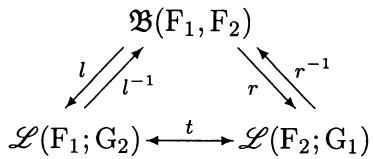
\includegraphics[keepaspectratio]{images/part003_fb3d81cd.jpg}}

其中 t 是转置同构 \(u \mapsto {}^{t}u\) 。鉴于 \(G_{1}\) 与 \(G_{2}\) 上弱拓扑的定义，还可直接看出：当 \(\mathfrak{B}(F_{1}, F_{2})\) 、 \(\mathcal{L}(F_{1}; G_{2})\) 与 \(\mathcal{L}(F_{2}; G_{1})\) 装备逐点收敛拓扑时，前一图中的同构是拓扑向量空间结构之间的同构。

现在设 E 、 F 是两个 Hausdorff 局部凸空间， \(E'\) 、 \(F'\) 是它们的对偶；我们用 \(E_{\sigma}\) 、 \(F_{\sigma}\) 表示装备弱化拓扑 \(\sigma(\mathrm{E}, \mathrm{E}')\) 、 \(\sigma(\mathrm{F}, \mathrm{F}')\) 的空间 E 、 F ，用 \(E_{s}'\) 、 \(F_{s}'\) 表示空间 \(E'\) 、 \(F'\) （装备弱拓扑 \(\sigma(\mathrm{E}', \mathrm{E})\) 、 \(\sigma(\mathrm{F}', \mathrm{F})\) ）。于是，前面的注记在三个空间 \(\mathfrak{B}(\mathrm{E}_{\sigma}, \mathrm{F}_{s}')\) 、 \(\mathcal{L}(\mathrm{E}_{\sigma}; \mathrm{F}_{\sigma})\) 与 \(\mathcal{L}(\mathrm{F}_{s}'; \mathrm{E}_{s}')\) 之间建立了典范同构，也在三个空间 \(\mathfrak{B}(\mathrm{E}_{\sigma}, \mathrm{F}_{\sigma})\) 、 \(\mathcal{L}(\mathrm{E}_{\sigma}; \mathrm{F}_{s}')\) 与 \(\mathcal{L}(\mathrm{F}_{\sigma}; \mathrm{E}_{s}')\) 之间建立了典范同构。我们将注意到， \(\mathfrak{B}(\mathrm{E}_{\sigma}, \mathrm{F}_{\sigma})\) 也等于空间 \(\mathfrak{B}(\mathrm{E}, \mathrm{F})\) ，即 \(E \times F\) 上分别连续双线性型所成的空间（ E 与 F 装备其原来的拓扑），因为 E （相应地， F ）上的每个连续线性形式在 \(E_{\sigma}\) （相应地， \(F_{\sigma}\) ）上连续，反之亦然（TVS, II, §6, No.~1 与 No.~2, 命题 3）。

设 \(\mathcal{B}(\mathrm{E},\mathrm{F})\) 是 \(\mathbf{E}\times \mathbf{F}\) 上连续双线性型所成的空间（ E 与 F 装备其原来的拓扑）；则 \(\mathcal{B}(\mathrm{E},\mathrm{F})\subset \mathfrak{B}(\mathrm{E},\mathrm{F})\) 。

命题 1. --- 双线性型 \(\Phi \in \mathfrak{B}(\mathrm{E},\mathrm{F})\) 属于 \(\mathcal{B}(\mathrm{E},\mathrm{F})\) 的充要条件是：存在 E 的一个 0 的邻域，它在 \(^l\Phi\) 下的像是 \(\mathbf{F}'\) 的一个等度连续子集。

因为，说 \(\Phi\) 连续，意思是存在 E （相应地， F ）中 0 的一个均衡凸邻域 V （相应地， W ），使得 \(|\Phi(x,y)| \leqslant 1\) （对 \(x \in V\) 、 \(y \in W\) ）；这可写成 \(|\langle^{l}\Phi(x), y \rangle| \leqslant 1\) （对 \(x \in V\) 、 \(y \in W\) ），或者写成 \(^{l}\Phi(V) \subset W^{\circ}\) ；由此即得命题，因为考虑到 \(F'\) 的每个等度连续子集都含于 F 中 0 的某个邻域的极集。

推论. --- 若 \(\Phi\) 是 \(\mathbf{E} \times \mathbf{F}\) 上的连续双线性型，则 \(^l\Phi\) 是 \(\mathbf{E}\) 到强对偶 \(\mathbf{F}_b'\) （ \(\mathbf{F}\) 的强对偶）中的连续线性映射。此外，若 \(\mathbf{E}\) 与 \(\mathbf{F}\) 是赋范空间，则 \(\|^l\Phi\| = \| \Phi \|\) 。

第一个断言由命题 1 以及 \(F_{b}^{\prime}\) 中 0 的每个邻域都吸收 \(F^{\prime}\) 的每个等度连续子集这一事实得出。若 E 与 F 赋范，则

\[
\begin{array}{c} \| \Phi \| = \sup _ {\| x \| \leqslant 1, \| y \| \leqslant 1} | \Phi (x, y) | = \sup _ {\| x \| \leqslant 1} \Big (\sup _ {\| y \| \leqslant 1} \big | \langle^ {l} \Phi (x), y \rangle \big | \Big) \\ = \sup _ {\| x \| \leqslant 1} \| ^ {l} \Phi (x) \| = \| ^ {l} \Phi \|, \end{array}
\]

由此得第二个断言。

交换 E 与 F 的角色，对线性映射 \(r\Phi\) 可得到与命题 1 及其推论类似的结果；我们把这些结果的叙述留给读者。

\section{具有性质（GDF）的几类空间}

我们已经知道每个 Fréchet 空间都具有性质（GDF）（TVS, I, §3, No.~3, 定理 1 的推论 5）。

命题 2. --- 设 E 是一个向量空间， \((\mathrm{F}_{\alpha})_{\alpha\in\mathrm{A}}\) 是具有性质（GDF）的局部凸空间的一个族，且对每个 \(\alpha\in A\) ，设 \(h_{\alpha}\) 是 \(F_{\alpha}\) 到 E 中的一个线性映射。若 E 装备使诸 \(h_{\alpha}\) 连续的最细局部凸拓扑，则 E 具有性质（GDF）。

设 \(u\) 是 \(\mathbf{E}\) 到一个 Banach 空间 \(\mathbf{B}\) 中的线性映射，使得在 \(\mathbf{E} \times \mathbf{B}\) 中，图 \(\Gamma\) （ \(u\) 的图）的点的每个收敛序列的每个极限也属于 \(\Gamma\) 。只需证明对每个 \(\alpha \in \mathbf{A}\) ， \(u \circ h_{\alpha}\) 在 \(\mathrm{F}_{\alpha}\) 上连续（TVS, II, §4, No.~4, 命题 5）。现在，设 \((x_n)\) 是 \(\mathrm{F}_{\alpha}\) 的元素的一个序列，具有极限 \(a\) ，且使得序列 \(\left(u(h_{\alpha}(x_n))\right)\) 具有一个极限 \(b \in \mathbf{B}\) 。由于 \(h_{\alpha}\) 连续， \(h_{\alpha}(a)\) 是序列 \((h_{\alpha}(x_n))\) 在 \(\mathbf{E}\) 中的一个极限；因此由假设 \(b = u(h_{\alpha}(a))\) ，且由于 \(\mathrm{F}_{\alpha}\) 具有性质（GDF）， \(u \circ h_{\alpha}\) 连续。

推论. --- 具有性质（GDF）的局部凸空间的每个商空间都具有性质（GDF）。

命题 3. --- 自反 Fréchet 空间的强对偶具有性质（GDF）。

这是命题 2 与下述引理（或 TVS, IV, §3, No.~4, 命题 4）的推论：

引理. --- 设 F 是一个 Fréchet 空间， \(F'\) 是它的强对偶， \(F''\) 是它的双对偶。若 \(F''\) 的每个关于 \(\sigma(F'', F')\) 有界的子集都含于 F 的一个有界子集的闭包（关于 \(\sigma(F'', F')\) ）中，则 \(F'\) 是 Banach 空间的一个序列的直接极限。

因为，设 \((\mathrm{V}_{n})\) 是 F 中 0 的凸、均衡、闭邻域的一个递减的基本序列。对每个整数 n ，设 \(G_{n}\) 是 \(F'\) 的线性子空间，由极集 \(V_{n}^{\circ}\) （ \(V_{n}\) 的极集）生成。在 \(G_{n}\) 中， \(V_{n}^{\circ}\) 是一个吸收性凸集，因此它的度规 \(p_{n}\) 是 \(G_{n}\) 上的一个范数；此外， \(V_{n}^{\circ}\) 是强对偶 \(F'\) 的完备子集（TVS, III, §3, No.~8, 命题 11）；从而 \(G_{n}\) （装备范数 \(p_{n}\) ）是一个 Banach 空间（GT, III, §3, No.~5, 命题 9 的推论 2）。我们将证明 \(F'\) 上的强拓扑是诸 \(G_{n}\) 上这些 Banach 空间拓扑的直接极限，或者等价地说，一个强闭、均衡、凸子集 U （ \(F'\) 的子集）是 0 的强邻域，当且仅当它吸收每个 \(V_{n}^{\circ}\) 。这个条件是必要的，这是显然的；为看出它是充分的，只需证明 U 含有 \(F'\) 的一个桶。事实上，此时它的极集 \(U^{\circ}\) （在 \(F''\) 中）将关于 \(\sigma(\mathrm{F}''\mathrm{,}\mathrm{F}')\) 有界，因而由假设含于 F 的某个有界子集 B 的闭包（关于 \(\sigma(\mathrm{F}''\mathrm{,}\mathrm{F}')\) ）中，由此可以断定 U （它关于 \(\sigma(\mathrm{F}^{\prime},\mathrm{F}''\mathrm{)})\) 是闭的）含有 0 的强邻域 \(B^{\circ}\) （TVS, II, §6, No.~3, 定理 1 与 §8, No.~4）。

由假设，对每个整数 n 存在一个数 \(\lambda_{n}>0\) ，使得 \(\lambda_{n}V_{n}^{\circ}\subset\frac{1}{2}U\) ；设 \(A_{n}\) 是诸 \(\lambda_{i}V_{i}^{\circ}\) （ \(i\leqslant n\) ）的并的凸包。则对每个 n 有 \(A_{n}\subset\frac{1}{2}U\) ；设 W 是诸 \(A_{n}\) 的并； W 是含于 \(\frac{1}{2}U\) 中的一个凸、均衡、吸收集，只需证明它的强闭包（它是一个桶）含于 U 中。

于是，设 \(x'\) 是 \(F'\) 中不属于 U 的一个点。由于每个 \(V_n^\circ\) 关于 \(\sigma(F', F)\) 是紧的，每个 \(A_n\) 亦然（TVS, II, §2, No.~6, 命题 15），且由于 \(x' \notin 2A_n\) ，存在一个元素 \(x_n\) ，它属于 \(A_n\) 在 F 中的极集，使得 \(\langle x', x_n \rangle = 2\) （TVS, II, §5, No.~3, 命题 4）。序列 \((x_n)\) 在 F 中有界：因为每个 \(y' \in F'\) 都属于某个 \(V_k^\circ\) ，于是 \(|\langle y', x_n \rangle| \leqslant \lambda_k^{-1}\) （对 \(n \geqslant k\) ），由此得我们的断言（TVS, IV, §1, No.~1, 命题 1）。设 C 是 F 中包含所有 \(x_n\) 的一个有界、均衡凸集；则 \(C^\circ\) 是 \(F'\) 中 0 的一个邻域，而极集 \(C^{\circ\circ}\) （ \(C^\circ\) 在 \(F''\) 中的极集）关于 \(\sigma(F'', F')\) 是紧的（TVS, III, §3, No.~4, 命题 4 的推论 2 与 No.~5, 命题 7）。于是可以看出，序列 \((x_n)\) 有一个聚点 \(x''\) （在 \(F''\) 中，关于 \(\sigma(F'', F')\) ）；显然 \(\langle x', x'' \rangle = 2\) ，而另一方面， \(x''\) 属于 \(A_n\) 在 \(F''\) 中的极集（对每个 \(n\) ），从而属于极集 \(W^\circ\) （ W 在 \(F''\) 中的极集）。由此得出 \(x' \notin W^{\circ\circ}\) ，因而 x' 不在 W 关于 \(\sigma(F', F'')\) 的闭包中（TVS, II, §6, No.~3, 定理 1 与 §8, No.~4），从而更不在强拓扑的闭包中，证明至此完成。

\chapter*{习题}
\phantomsection
\addcontentsline{toc}{chapter}{习题}
\setcounter{exercisegroup}{1}
\edef\CurrentExerciseGroup{\arabic{exercisegroup}}
\section*{\texorpdfstring{\S\CurrentExerciseGroup}{第{\CurrentExerciseGroup}节}}
\phantomsection
\addcontentsline{toc}{section}{第{\CurrentExerciseGroup}节习题}

\begin{enumerate}
\def\labelenumi{\arabic{enumi})}
\item
  考察与区间 {[}0, 1{]} 相同的局部紧空间 T、T'，以及 T 与 T' 上分别与 Lebesgue 测度相同的测度 \(\mu, \mu'\)。设 F 是一个 Hilbert 空间，具有可数标准正交基，并将其排成双重序列 \((\mathbf{e}_{mn})\)；设 F' = F 为其对偶。令 \(\mathbf{u}_m(t) = \mathbf{e}_{mn}\)，适用于 \((n-1)2^{-m} \leqslant t < n2^{-m}\) 与 \(1 \leqslant n \leqslant 2^m\)；令 \(\mathbf{f}(t, t') = 2^m \mathbf{u}_m(t)\)，适用于 \(2^{-m} < t' \leqslant 2^{-m+1}\)，最后令 \(\mathbf{f}(t, 0) = 0\) 与 \(\mathbf{f}(1, t') = 0\)。试证 \(\mathbf{f}\) 关于乘积测度 \(\mu \otimes \mu'\) 是标量可积的，但函数 \(t' \mapsto \mathbf{f}(t, t')\) 不是标量 \(\mu'\)-可积的——对任何 \(t \in T\) 都是如此。
\item
  设 \(\mathrm{T}, \mathrm{X}, \mathrm{Y}\) 是三个局部紧空间，其中 \(\mathrm{Y}\) 具有可数基。设 \(\mu\) 是一个测度 \(\geqslant 0\)，定义在 \(\mathrm{T}\) 上；设 \(t \mapsto \lambda_t (t \in \mathrm{T})\) 是一个 \(\mu\)-适宜\(^1\) 的测度族，\(\geqslant 0\)，定义在 \(\mathrm{X}\) 上，并令 \(\nu = \int \lambda_t d\mu(t)\)。设 \(x \mapsto \rho_x (x \in \mathrm{X})\) 是一个 \(\nu\)-适宜的测度族，\(\geqslant 0\)，定义在 \(\mathrm{Y}\) 上。此外，假设还满足下列两个条件之一：a) \(\mathrm{X}\) 是无穷远处可数的；
\end{enumerate}

\begin{enumerate}
\def\labelenumi{\alph{enumi})}
\setcounter{enumi}{1}
\tightlist
\item
  \(\nu\) 是有界的。
\end{enumerate}

在这些条件下，试证存在一个局部 \(\mu\)-可忽略集 \(N'\)，使得对每个 \(t \notin N'\)，族 \(x \mapsto \rho_x\) 都是 \(\lambda_t\)-适宜的；此外，族 \(t \mapsto \int \rho_x d\lambda_t(x)\)（对 \(t \notin N'\) 有定义）是 \(\mu\)-适宜的，且

\[
\int d \mu (t) \int \rho_ {x} d \lambda_ {t} (x) = \int \rho_ {x} d \nu (x).
\]

（为证 \(x \mapsto \rho_x\) 局部几乎处处为标量 \(\lambda_t\)-可积，可利用 §3 第 1 号的引理 1，在情形 \(b\) 中要利用 \(\lambda_t\) 局部几乎处处有界这一事实；用同样的方法可证 \(t \mapsto \int \rho_x d\lambda_t(x)\) 是标量 \(\mu\)-可积的；再利用第 5 号的命题 13。）

\begin{enumerate}
\def\labelenumi{\arabic{enumi})}
\setcounter{enumi}{2}
\tightlist
\item
  设 S、T、Y 是三个无穷远处可数的局部紧空间，且 Y 具有可数基。设 \(\rho\)（相应地 \(\sigma\)）是 S（相应地 T）上的正测度，\(\nu = \rho \otimes \sigma\)，并设 \((\lambda_{s,t})_{(s,t) \in \mathbb{S} \times \mathbb{T}}\) 是 Y 上的一个 \(\nu\)-适宜\(^{1}\)正测度族。那么，存在一个 \(\rho\)-可忽略集 N，使得对每个 \(s \notin N\)，族 \((\lambda_{s,t})_{t \in \mathbb{T}}\) 都是 \(\sigma\)-适宜的；族 \(s \mapsto \int \lambda_{s,t} d\sigma(t)\)（几乎处处有定义）是 \(\rho\)-适宜的，且
\end{enumerate}

\[
\iint \lambda_ {s, t} d \rho (s) d \sigma (t) = \int d \rho (s) \int \lambda_ {s, t} d \sigma (t).
\]

（对空间 \(\mathrm{X} = \mathrm{S} \times \mathrm{T}\) 应用习题 2，并注意 \(\nu = \int (\varepsilon_s \otimes \sigma) d\rho(s)\)。）

\begin{enumerate}
\def\labelenumi{\arabic{enumi})}
\setcounter{enumi}{3}
\tightlist
\item
  设 \(\mathrm{T}, \mathrm{X}, \mathrm{Y}\) 是三个局部紧空间，其中 \(\mathrm{X}\) 是无穷远处可数的。设 \(\mu\) 是 \(\mathrm{T}\) 上的正测度，\((\lambda_t)_{t \in \mathrm{T}}\) 是一个 \(\mu\)-适宜正测度族（在 \(\mathrm{X}\) 上），且 \(\nu = \int \lambda_t d\mu(t)\)。假设下列两个条件之一成立：
\end{enumerate}

\begin{enumerate}
\def\labelenumi{\alph{enumi})}
\item
  Y 具有可数基；
\item
  测度 \(\nu\) 是有界的。
\end{enumerate}

在这些条件下，若 \(\pi\) 是 X 到 Y 中的 \(\nu\)-逆紧映射，则诸 \(t \in \mathbf{T}\) 中使 \(\pi\) 不是 \(\lambda_t\)-逆紧者所成之集是局部 \(\mu\)-可忽略的；此外，Y 上的正测度族 \((\pi(\lambda_t))_{t \in \mathbf{T}}\)（在 T 中局部几乎处处有定义）是 \(\mu\)-适宜的，且

\[
\pi \left(\int \lambda_ {t} d \mu (t)\right) = \int \pi (\lambda_ {t}) d \mu (t).
\]

（在情形 \(a\)，对 \(\rho_x = \varepsilon_{\pi(x)}\) 应用习题 2。在情形 \(b\)，注意 \(\lambda_t\) 局部几乎处处有界，于是可归结为证明映射 \(t \mapsto \pi(\lambda_t)\) 是淡 \(\mu\)-可测的（参见第 V 章 §3 第 2 号命题 4）。给定一个数 \(\varepsilon > 0\)，并设 \(K\) 是 \(T\) 的紧子集，首先注意 \(X\) 中存在递增的紧集序列 \((F_m)\)，使 \(\pi\) 在每个 \(F_m\) 上的限制连续，且令 \(N_m = X - F_m\) 时有 \(\nu(N_m) \leqslant \varepsilon/4^m\)。设 \(A_m\) 是 \(t \in K\) 中使 \(N_m\) 不是 \(\lambda_t\)-可积或使 \(\lambda_t(N_m) > 1/2^m\) 的那些 t 所成的集；若 \(A\) 是诸 \(A_m\) 之并，则 \(\mu(A) \leqslant \varepsilon/2\)。设 \(K_1\) 是 \(K - A\) 的紧子集，使 \(\mu(K - K_1) \leqslant \varepsilon\)，且对每个函数 \(g \in \mathcal{H}(X)\)，\(t \mapsto \int g(x) d\lambda_t(x)\) 在 \(K_1\) 上的限制连续。利用 Urysohn 定理，试证对每个函数 \(f \in \mathcal{H}(Y)\)，在 \(K_1\) 上 \(t \mapsto \int f(\pi(x)) d\lambda_t(x)\) 的限制是连续函数的一致极限。）

*5) 对每个 \(t \in \mathbf{R}\)，令 \(\mathbf{f}(t)\) 为连续函数 \(x \mapsto \exp(-2\pi itx)\)，它是空间 \(\mathcal{C} = \mathcal{C}_{\mathbf{C}}(\mathbf{R})\)（\(\mathbf{R}\) 上的连续复函数空间）中的一个元素。空间 \(\mathcal{C}\) 与空间 \(\mathcal{C}' = \mathcal{C}'_{\mathbf{C}}(\mathbf{R})\)（\(\mathbf{R}\) 上具有紧支集的复测度组成的空间）成对偶；具有紧支集的连续复函数空间 \(\mathcal{K} = \mathcal{K}_{\mathbf{C}}(\mathbf{R})\) 可按典范方式与 \(\mathcal{C}'\) 的一个子空间等同，办法是把函数 \(\varphi \in \mathcal{K}\) 等同于关于 Lebesgue 测度以 \(\varphi\) 为密度的测度。用 \(\mathcal{D}\) 表示由 \(\mathcal{K}\) 中具有紧支集的无穷次可微复函数所构成的子空间。试证：当 \(\mathcal{C}\) 赋予拓扑 \(\sigma(\mathcal{C},\mathcal{C}')\) 或拓扑 \(\sigma(\mathcal{C},\mathcal{K})\) 时，\(\mathbf{f}\) 关于 Lebesgue 测度 \(\mu\) 不是标量可积的；然而对拓扑 \(\sigma(\mathcal{C},\mathcal{D})\)，\(\mathbf{f}\) 是标量 \(\mu\)-可积的，且 \(\int f d\mu\) 是测度 \(\varepsilon_0\)；试证在此情形命题 7 的条件得到验证。*

\begin{enumerate}
\def\labelenumi{\arabic{enumi})}
\setcounter{enumi}{5}
\item
  设 F 是一个可分辨的 Fréchet 空间（TVS，IV，§2，习题 4 b）），F' 是其对偶。试证：若 f 是 T 到 F 中的标量本质可积映射，则 \(\int f d\mu\) 属于 F 的双对偶 F'\,'。（把 F 嵌入 F'\,'；应用定理 1 以及命题 2 与附录的引理。）
\item
  \begin{enumerate}
  \def\labelenumii{\alph{enumii})}
  \tightlist
  \item
    设 \(\mathbf{F} = \overline{\mathcal{K}(\mathbf{N})}\) 是趋于 0 的实数序列组成的 Banach 空间，\(\mathbf{F}' = \mathbf{L}^1 (\mathbf{N})\) 是其对偶（TVS，IV，§1，习题 1）。设 \(\mathbf{f} = (f_n)\) 是 \(\mathrm{I} = [0,1]\) 到 \(\mathbf{F}\) 中的映射，满足 \(f_{n}(t) = n\varphi_{\mathrm{I}_{n}}(t)\)，其中 \(\mathrm{I}_n = [0,1 / n]\)。试证 \(\mathbf{f}\) 关于 Lebesgue 测度 \(\mu\)（在 \(\mathrm{I}\) 上）是标量可积的，但 \(\int \mathbf{f}d\mu\) 是 \(\mathbf{F}''\) 中不属于 \(\mathbf{F}\) 的元素。
  \end{enumerate}
\end{enumerate}

\begin{enumerate}
\def\labelenumi{\alph{enumi})}
\setcounter{enumi}{1}
\item
  设 \(\mathbf{g}\) 是 \(J = [-1, +1]\) 到 \(F\) 中的映射，由条件 \(\mathbf{g}(t) = \mathbf{f}(t)\)（对 \(t \geqslant 0\)）与 \(\mathbf{g}(t) = -\mathbf{f}(-t)\)（对 \(t \leqslant 0\)）定义。则 \(\mathbf{g}\) 关于 \(J\) 上的 Lebesgue 测度是标量可积的，且 \(\int \mathbf{g} d\mu \in F\)，但存在函数 \(h \in \mathcal{L}^{\infty}\) 使 \(\int h\mathbf{g} d\mu \notin F\)。
\item
  由 \(a\) 推出拓扑向量空间 \(F\) 不与任何赋范空间的对偶同构这一事实的一个新证明（TVS，IV，§2，习题 22 c））。
\end{enumerate}

\begin{enumerate}
\def\labelenumi{\arabic{enumi})}
\setcounter{enumi}{7}
\tightlist
\item
  设 \(\mathbf{F}\) 是一个 Hausdorff 局部凸空间，\(\mathbf{f}\) 是 \(\mathbf{T}\) 到 \(\mathbf{F}\) 中的标量局部可积映射，使得对每个紧子集 \(\mathbf{K}\)（\(\mathbf{T}\) 中的）都有 \(\int_{\mathbf{K}} \mathbf{f} d\mu \in \mathbf{F}\)。
\end{enumerate}

\begin{enumerate}
\def\labelenumi{\alph{enumi})}
\item
  试证：若 \(\mathbf{f}\) 是标量本质可积的，且 \(\mathrm{F}\) 是半自反的（或者只需每个对 \(\sigma (\mathrm{F},\mathrm{F}^{\prime})\) 的 Cauchy 序列对该拓扑都在 \(\mathrm{F}\) 中收敛，当 \(\mathrm{T}\) 是无穷远处可数时），则 \(\int g\mathbf{f}d\mu \in \mathrm{F}\) 对每个函数 \(g\in \mathcal{L}^{\infty}\) 成立。
\item
  试证：若 F 是拟完备的，且对 F 上每个连续半范数 q 都有 \(\int^{\bullet} q(\mathbf{f}(t)) d\mu(t) < +\infty\)，则 f 是标量本质可积的，且 \(\int g\mathbf{f} d\mu \in F\) 对每个函数 \(g \in L^{\infty}\) 成立。
\end{enumerate}

（在两种情形中，都考察 T 的紧子集组成的递增有向集。）

\begin{enumerate}
\def\labelenumi{\arabic{enumi})}
\setcounter{enumi}{8}
\item
  设 G、H 是两个 Hausdorff 局部凸空间，U 是 T 到 \(F = \mathcal{L}_{s}(G;H)\) 中的映射。假设 G 是桶式的，H 是拟完备的，U 是 \(\mu\)-可测的，且对 T 的每个紧子集 K，\(U(K)\) 都有界；此外还假设，对 H 上每个连续半范数 q 以及每个 \(x \in G\)，\(\int^{\bullet} q(U(t) \cdot x) d\mu(t) < +\infty\)。在这些条件下，试证 U 是标量本质 \(\mu\)-可积的，且 \(\int U(t) d\mu(t) \in F\)（利用习题 8 b））。
\item
  设 \(G, H\) 是两个 Fréchet 空间，\(G_0\)（相应地 \(H_0\)）是 \(G\)（相应地 \(H\)）的稠密子集，\(t \mapsto \Phi_t\) 是 \(T\) 到空间 \(F = \mathcal{B}(G, H)\)（即 \(G \times H\) 上连续双线性型组成的空间，赋以逐点收敛拓扑）中的映射。假设：\(1^\circ\) 对每个对 \((a, b) \in G_0 \times H_0\)，\(t \mapsto \Phi_t(a, b)\) 都是本质 \(\mu\)-可积的；\(2^\circ\) 若对每对有界子集 \(A \subset G\)、\(B \subset H\)，令 \(q_{A,B}(\Phi) = \sup_{(x, y) \in A \times B} |\Phi(x, y)|\)，其中
\end{enumerate}

对每个 \(\Phi \in \mathcal{B}(\mathrm{G},\mathrm{H})\) 都有 \(\int^{*}q_{\mathrm{A},\mathrm{B}}(\Phi_t)d\mu (t) < + \infty\)。在这些条件下，试证 \(t\mapsto \Phi_t\) 是标量本质 \(\mu\)-可积的，且 \(\int \Phi_t d\mu (t)\in \mathrm{F}\)（利用 Lebesgue 定理，归结为应用定理 1 的推论 1）。\(\mathrm{H} = \mathbf{R}\) 的特殊情形。

\begin{enumerate}
\def\labelenumi{\arabic{enumi})}
\setcounter{enumi}{10}
\item
  设 \(\mu\) 是 \(T = [0,1]\) 上的 Lebesgue 测度，\(F\) 是具有可数标准正交基 \((\mathbf{e}_n)\) 的 Hilbert 空间。设 \(\mathbf{f}\) 是 \(T\) 到 \(F\) 中的映射，满足 \(\mathbf{f}(0) = 0\)，且 \(\mathbf{f}(t) = 2^n \mathbf{e}_n / n\) 在区间 \([2^{-n-1}, 2^{-n}]\) 上成立（\(n \geqslant 0\)）。试证 \(\mathbf{f}\) 是 \(\mu\)-可测的、标量 \(\mu\)-可积的，且 \(\int \mathbf{f} d\mu \in F\)，但 \(\int^* |\mathbf{f}| d\mu = +\infty\)。
\item
  设 \(\mu\) 是 \(T = [0,1]\) 上的 Lebesgue 测度，并设 \(F\) 是一个 Hilbert 空间，具有标准正交基 \((\mathbf{e}_t)_{t \in T}\)，与 \(T\) 等势。
\end{enumerate}

\begin{enumerate}
\def\labelenumi{\alph{enumi})}
\item
  设 \(\mathbf{f}\) 是映射 \(t \mapsto \mathbf{e}_t\)，从 \(\mathrm{T}\) 到 \(\mathrm{F}\) 中。试证 \(\mathbf{f}\) 是标量 \(\mu\)-可忽略的，但不是 \(\mu\)-可测的（当 \(\mathrm{F}\) 赋以弱拓扑 \(\sigma(\mathrm{F}, \mathrm{F}')\) 时；更不用说当 \(\mathrm{F}\) 赋以其原拓扑时了）。
\item
  设 A 是 T 中的一个不可测集（第 IV 章 §4，习题 8）；试证函数 \(\mathbf{g} = \mathbf{f}\varphi_{\mathrm{A}}\) 是标量 \(\mu\)-可忽略的，但数值函数 \(|\mathbf{g}|\) 不是 \(\mu\)-可测的。
\end{enumerate}

\begin{enumerate}
\def\labelenumi{\arabic{enumi})}
\setcounter{enumi}{12}
\item
  设 F 是 Hausdorff 局部凸空间，\(F'\) 是其对偶，q 是 F 上的一个下半连续半范数。试证：若 f 是 T 到 F 中的映射，是 \(\mu\)-可测的（对拓扑 \(\sigma(\mathrm{F},\mathrm{F}')\)），则数值函数 \(q \circ f\) 是 \(\mu\)-可测的。
\item
  设 \(\mu\) 是 T = {[}0,1{]} 上的 Lebesgue 测度；用 F 表示由 T 上有限的 \(\mu\)-可测数值函数组成的 R 上的向量空间，赋以逐点收敛拓扑，这使它成为一个 Hausdorff 局部凸空间。
\end{enumerate}

\begin{enumerate}
\def\labelenumi{\alph{enumi})}
\item
  试证 F 中存在可数稠密子集（考察 T 上连续数值函数组成的 Banach 空间 \(\mathcal{C}(T)\) 中的一个稠密序列）。
\item
  对每个 \(t \in T\)，令 \(\mathbf{f}(t)\) 是 F 的对偶 \(F'\) 中由 \(\langle\mathbf{f}(t), z\rangle = z(t)\)（对一切 \(t \in T\)）定义的元素。试证：当 \(F'\) 赋以拓扑 \(\sigma(\mathrm{F}', \mathrm{F})\) 时，f 是标量 \(\mu\)-可测的，但不是 \(\mu\)-可测的（参见命题 13）。
\end{enumerate}

\begin{enumerate}
\def\labelenumi{\arabic{enumi})}
\setcounter{enumi}{14}
\item
  设 F 是可度量化的局部凸空间，f 是 T 到 F 中的标量 \(\mu\)-可测映射，使得对 T 的每个紧子集 K，存在 F 的可数子集 H，使 \(\mathbf{f}(t) \in \overline{\mathbf{H}}\) 对几乎所有的 \(t \in K\) 成立；试证在这些条件下，f 对 F 的原拓扑是 \(\mu\)-可测的。（在化归到 F 为可分的情形之后，把 F 嵌入可数个赋范空间的乘积中。）
\item
  设 \(\mathbf{F}\) 是 Banach 空间，\(\mathbf{F}'\) 是其对偶。对每个 \(p\)，当 \(1 \leqslant p \leqslant +\infty\) 时，用 \(\Lambda_{\mathbf{F}'}^p(\mathrm{T},\mu)\)（或简记为 \(\Lambda_{\mathbf{F}'}^p\)）表示由这样的映射 \(\mathbf{f}\)——即 \(\mathrm{T}\) 到 \(\mathbf{F}'\) 中的、使得对每个 \(\mathbf{z} \in \mathbf{F}\) 数值函数 \(\langle \mathbf{z},\mathbf{f}\rangle\) 属于 \(\mathcal{L}^p(\mathrm{T},\mu)\) 的映射——组成的集。有 \(\Lambda_{\mathbf{F}'}^p \supset \mathcal{L}_{\mathbf{F}'}^p\)，且 \(\Lambda_{\mathbf{F}'}^1\) 是标量本质 \(\mu\)-可积的、取值于 \(\mathbf{F}'\) 的函数组成的空间（\(\mathbf{F}'\) 赋以 \(\sigma(\mathbf{F}',\mathbf{F})\)）。已知，若用 \(\theta(\mathbf{z})\) 表示 \(\langle \mathbf{z},\mathbf{f}\rangle\) 在 \(\mathrm{L}^p(\mu)\) 中的类，则映射 \(\mathbf{z} \mapsto \theta(\mathbf{z})\) 是连续的（第 4 号，引理 2）；设 \(M_p(\mathbf{f})\) 为其范数；它是空间 \(\Lambda_{\mathbf{F}'}^p\) 上的一个半范数。为使 \(M_p(\mathbf{f}) = 0\)，必要且充分的是 \(\mathbf{f}\) 为标量局部可忽略的。
\end{enumerate}

\begin{enumerate}
\def\labelenumi{\alph{enumi})}
\item
  为使 \(\mathbf{f} \in \Lambda_{\mathbf{F}'}^p\)，必要且充分的是：对每个数值函数 \(g \in \mathcal{L}^q\)，函数 \(g\mathbf{f}\) 都是标量本质 \(\mu\)-可积的；此时有 \(\mathrm{M}_1(g\mathbf{f}) \leqslant \mathrm{M}_p(\mathbf{f})\mathrm{N}_q(g)\)。
\item
  在空间 \(\Lambda_{\mathbf{F}'}^1\) 中，试证半范数 \(\mathbf{M}_1\) 等价于半范数 \(\mathrm{M}_1'(\mathbf{f}) = \sup |\int_{\mathbf{A}} \mathbf{f} d\mu|\)，其中 A 取遍 T 的可测子集所成的集；更精确地，\(\mathrm{M}_1' \leqslant \mathrm{M}_1 \leqslant 2\mathrm{M}_1'\)。由此推出 \(\mathrm{M}_p\) 是等价于 \(\mathrm{M}_p'(\mathbf{f}) = \sup_{\mathrm{N}_q(g) \leqslant 1} \mathrm{M}_1'(g\mathbf{f})\) 的半范数。
\item
  取 F 为一个具有可数标准正交基的 Hilbert 空间，取 \(\mu\) 为 \(T = [0,1]\) 上的 Lebesgue 测度。试证存在 T 到 F 中的一个映射，它不可积但标量可积，并且是可测阶梯函数序列在半范数 \(M_1\) 下的极限（参见习题 11）；由此推出：在空间 \(\mathcal{L}_{\mathrm{F}}^1\)（即 \(\mu\)-可积函数组成的空间）上，由半范数 \(M_1\) 定义的拓扑严格粗于由 \(N_1\) 定义的拓扑。对半范数 \(M_p\) 与 \(N sub p\)（\(1 \leqslant p < +\infty\)）有类似的结果。
\end{enumerate}

\(d\)）试证：在空间 \(\mathcal{L}_{\mathrm{F}^{\prime}}^{\infty}\) 上，\(\mathrm{M}_{\infty} = \mathrm{N}_{\infty}\)

\begin{enumerate}
\def\labelenumi{\alph{enumi})}
\setcounter{enumi}{4}
\tightlist
\item
  取 F 为一个具有可数标准正交基的 Hilbert 空间，该基排成双重序列 \((\mathbf{e}_{mn})\)。设 \(\mu\) 是 \(T = [0,1]\) 上的 Lebesgue 测度。设 \(\mathbf{u}_m\) 是 T 到 F 中的映射，满足 \(\mathbf{u}_m(t) = \mathbf{e}_{mn}\)（对 \((n - 1)2^{-m} \leqslant t < n2^{-m}\) 及 \(1 \leqslant n \leqslant 2^m\)），且 \(\mathbf{u}_m(1) = 0\)；令 \(\mathbf{f}_n = \sum_{i=0}^{n} \mathbf{u}_i\)。试证：对 \(1 \leqslant p < +\infty\)，\((\mathbf{f}_n)\) 是 \(\Lambda_{\mathrm{F}'}^p\) 中的 Cauchy 序列，但不收敛于 \(\Lambda_{\mathrm{F}'}^p\) 中的任何函数。
\end{enumerate}

\begin{enumerate}
\def\labelenumi{\alph{enumi})}
\setcounter{enumi}{5}
\item
  设 \((\mathbf{f}_{n})\) 是空间 \(\Lambda_{F'}^{p}\)（\(1 \leqslant p \leqslant +\infty\)）中的 Cauchy 序列；假设存在 T 到 \(F'\) 中的映射 f，使得对每个 \(z \in F\)，函数序列 \(\langle z, f_{n} \rangle\) 都依测度收敛于 \(\langle z, f \rangle\)（第 IV 章 §5 第 11 号）。试证 \(f \in \Lambda_{F'}^{p}\)，且序列 \((\mathbf{f}_{n})\) 在 \(\Lambda_{F'}^{p}\) 中以 f 为极限。
\item
  取 F 为绝对收敛级数组成的 Banach 空间 \(\mathrm{L}^{1}(\mathbf{N})\)；其对偶为 \(\mathbf{F}^{\prime} = \mathrm{L}^{\infty}(\mathbf{N})\)（TVS，IV，§1，习题 1）。设 \(\mu\) 是 T = {[}0,1{]} 上的 Lebesgue 测度。设 f 是 T 到 \(F^{\prime}\) 中的映射，满足 \(\mathbf{f}(0) = 0\)，且对 \(2^{-n-1} < t \leqslant 2^{-n}\)，\(\mathbf{f}(t)\) 是这样的序列：它的各项皆为零，除了指标为 n 的项等于 \(2^{n/p}\)（\(1 \leqslant p < +\infty\)）。试证 f 对 \(F^{\prime}\) 上的强拓扑是可测的，且属于 \(\Lambda_{\mathrm{F}'}^p\)，但任何阶梯函数序列 \((\mathbf{f}_n)\) 都不趋于 \(\mathbf{f}\)（在空间 \(\Lambda_{\mathrm{F}'}^p\) 中）。
\end{enumerate}

¶ 17) 设 \(\mu\) 是 \(T = [0,1]\) 上的 Lebesgue 测度，\(F\) 是 Banach 空间 \(L^1(\mathbf{N})\)，\(F' = L^\infty(\mathbf{N})\) 是其对偶。对每个 \(t \in [0,1[\)，设 \(t = \sum_{n=0}^\infty \xi_n 2^{-n}\) 为 \(t\) 的二进展开；用 \(f(t)\) 表示序列 \((\xi_n) \in F'\)，并令 \(f(1) = 0\)。

\begin{enumerate}
\def\labelenumi{\alph{enumi})}
\item
  试证：对 \(1 \leqslant p \leqslant +\infty\)，函数 \(\mathbf{f}\) 属于空间 \(\Lambda_{\mathrm{F}'}^p\)（参见习题 16）。
\item
  试证 \(\mathbf{f}\) 对拓扑 \(\sigma(\mathrm{F}',\mathrm{F})\) 是可测的，且对该拓扑存在一个阶梯函数序列几乎处处收敛于 \(\mathbf{f}\)。
\item
  试证 \(\mathbf{f}\) 对 \(\mathbf{F}'\) 上的强拓扑不是可测的（注意 \(|\mathbf{f}(t) - \mathbf{f}(t')| = 1\)，只要 \(0 \leqslant t < t' < 1\)）。
\item
  试证：在空间 \(\Lambda_{\mathrm{F}'}^p\)（\(1 \leqslant p < +\infty\)）中，\(\mathbf{f}\) 不是任何阶梯函数序列的极限。（可归结为只考虑这样的阶梯函数：它们是区间的特征函数的线性组合（系数取自 \(\mathbf{F}'\)），其中区间的端点形如 \(k/2^n\)；若 \(\mathbf{g}\) 是这样一个阶梯函数，试证在习题 16 b) 的记号下有 \(\mathrm{M}_1'(\mathbf{f} - \mathbf{g}) \geqslant 1/4\)。）
\item
  试证不存在任何映射 \(\mathbf{h}\)——\(\mathrm{T}\) 到 \(\mathrm{F}'\) 中的、对强拓扑可测的映射——使 \(\mathbf{f} - \mathbf{h}\) 是标量可忽略的。（注意对这样的映射，必然有 \(\mathrm{N}_{\infty}(\mathbf{h}) \leqslant 1\)；然后由此得出与 \(d\) 的结果矛盾。）
\end{enumerate}

\begin{enumerate}
\def\labelenumi{\arabic{enumi})}
\setcounter{enumi}{17}
\tightlist
\item
  试证：当把 \(\mathbf{f}\) 为 \(\mu\)-可测（对 \(\mathbf{F}\) 的原拓扑）这一条件换成 \(\mathbf{f}\) 为 \(\mu\)-可测（对弱化拓扑 \(\sigma(\mathrm{F},\mathrm{F}')\)）这一条件时，命题 8 仍然成立。（利用第 IV 章 §4 习题 19 c）。）
\end{enumerate}

¶ 19) 设 f 是 T 到 F 中的标量本质 μ-可积映射。对每个 \(z' \in F'\)，用 \(u_{\mathbf{f}}(\mathbf{z}')\) 表示 \(L^{1}(\mu)\) 中由函数 \(\langle f, z' \rangle\) 所确定的类。若对每个函数 \(g \in L^{\infty}(\mu)\) 都有 \(\int g f d\mu \in F\)，则称 f 是标量良可积的。

\begin{enumerate}
\def\labelenumi{\alph{enumi})}
\item
  为使 \(\mathbf{f}\) 是标量良可积的，必要且充分的是 \(u_{\mathbf{f}}\) 对拓扑 \(\sigma(\mathrm{F}',\mathrm{F})\) 与 \(\sigma(\mathrm{L}^1,\mathrm{L}^\infty)\) 连续。当此条件成立时，在 \(u_{\mathbf{f}}\) 之下，\(\mathrm{F}'\) 的每个等度连续子集的像是 \(\mathrm{L}^1\) 中的相对弱紧子集。特别地：\(\alpha\) 对每个等度连续子集 \(\mathrm{H}'\)（\(\mathrm{F}'\) 的）以及每个 \(\varepsilon >0\)，存在紧子集 \(\mathrm{L}\)（在 \(\mathrm{T}\) 中），使 \(\int_{\mathrm{T}-\mathrm{L}}|\langle\mathbf{f},\mathbf{z}'\rangle|d\mu\leqslant\varepsilon\) 对一切 \(\mathbf{z}'\in\mathrm{H}'\) 成立；\(\beta\) 对每个等度连续子集 \(\mathrm{H}'\)（\(\mathrm{F}'\) 的）以及每个 \(\varepsilon>0\)，存在 \(\eta>0\)，使得对每个开集 \(\mathrm{U}\subset\mathrm{T}\)（测度 \(\mu(\mathrm{U})\leqslant\eta\)），都有 \(\int_{\mathrm{U}}|\langle\mathbf{f},\mathbf{z}'\rangle|d\mu\leqslant\varepsilon\) 对一切 \(\mathbf{z}'\in\mathrm{H}'\) 成立（第 V 章 §5，习题 15）。
\item
  假设条件 \(\alpha\) 与 \(\beta\)（\(a\) 中的）都成立，此外还存在子空间 \(\mathrm{H} \subset \mathrm{L}^{\infty}\)，它对拓扑 \(\sigma(\mathrm{L}^{\infty}, \mathrm{L}^{1})\) 稠密，使得对每个函数 \(g \in \mathcal{L}^{\infty}\)，只要其类属于 \(\mathrm{H}\)，就有 \(\int g\mathbf{f}d\mu \in \mathrm{F}\)。试证在这些条件下，若再假设 \(\mathrm{F}\) 是拟完备的，则 \(\mathbf{f}\) 是标量良可积的。（先化归到 \(\mathrm{F}\)（对其原拓扑）完备的情形，并注意 \(\dot{g} \mapsto \int g\mathbf{f}d\mu\) 是 \(\mathrm{L}^{\infty}\) 到 \(\mathrm{F}'*\) 中的连续线性映射，其中 \(\mathrm{L}^{\infty}\) 赋以拓扑 \(\tau(\mathrm{L}^{\infty}, \mathrm{L}^{1})\)，\(\mathrm{F}'*\) 赋以在 \(\mathrm{F}'\) 的等度连续子集上一致收敛的拓扑。）
\item
  设 \(\mathbf{f}\) 是标量良可积的。试证对每个 Cauchy 序列 \((\mathbf{z}_n')\)（对拓扑 \(\sigma(\mathrm{F}',\mathrm{F})\)），序列 \((u_{\mathbf{f}}(\mathbf{z}_n'))\) 在 \(\mathrm{L}^1\) 中强收敛（利用第 IV 章 §5 习题 25 c) 与第 V 章 §5 习题 16 b)）。由此推出：若 A 是 \(\mathrm{L}^{\infty}\) 的单位球在映射 \(\dot{g} \mapsto \int g\mathbf{f}d\mu\) 下的像，则每个 Cauchy 序列 \((\mathbf{z}_n')\)（对拓扑 \(\sigma(\mathrm{F}',\mathrm{F})\)）都是对在 A 上一致收敛的拓扑的 Cauchy 序列。
\end{enumerate}

\(d)\) 由 \(c)\) 推出：若 \(\mathbf{f}\) 是标量良可积的，则 \(u_{\mathbf{f}}\) 把 \(\mathrm{F}'\) 的每个对 \(\sigma (\mathrm{F}',\mathrm{F})\) 等度连续且可度量化的子集映为 \(L^{1}\) 中的相对强紧集。特别地，若 F 是 Hausdorff 局部凸空间 G 的对偶 \(G'\)，F 赋以一个与 F 和 G 之间的对偶相容的拓扑，且 \(G'\) 中存在可数的强稠密集，则 \(u_{f}\) 把 \(F' = G\) 的每个有界子集映为 \(L^{1}\) 中相对强紧的集（把 G 嵌入其双对偶）。

\begin{enumerate}
\def\labelenumi{\arabic{enumi})}
\setcounter{enumi}{19}
\tightlist
\item
  设 F 是 Hausdorff 局部凸空间，\(F'\) 是其对偶，\(S'\) 是由这样的子集 \(A' \subset F'\) 组成的集：\(A'\) 的每个点序列都有对 \(\sigma(\mathrm{F}',\mathrm{F})\) 收敛的子序列。试证：对 F 的有界子集 A，下列条件等价：\(\alpha\) A 对 \(S'\)-拓扑是预紧的；\(\beta\) 每个对 \(\sigma(\mathrm{F}',\mathrm{F})\) 收敛的序列都在 A 上一致收敛。（设 S 是由 F 与 A 的有限子集组成的集；注意 \(\beta\) 蕴含每个集 \(A' \in S'\) 对 S-拓扑是预紧的，这里要用 GT，II，§4 习题 6。然后应用 TVS，IV，§1 习题 4。）
\end{enumerate}

¶ 21) 设 f 是 T 到拟完备 Hausdorff 局部凸空间 F 中的标量良可积映射。

\begin{enumerate}
\def\labelenumi{\alph{enumi})}
\item
  试证在下列每种情形中，映射 \(\dot{g} \mapsto \int g\mathbf{f}  d\mu\) 把 \(\mathrm{L}^{\infty}\) 的单位球映为 \(\mathbf{F}\) 中对原拓扑的相对紧子集：\(1^{\circ}\) \(\mathbf{F}\) 中存在可数稠密集；\(2^{\circ}\) \(\mathbf{F}\) 是一个对偶 \(\mathbf{G}'\)——其中 \(\mathbf{G}\) 或者可度量化，或者是可度量化空间序列的严格直接极限——且 \(\mathbf{F}\) 赋以拓扑 \(\tau (\mathbf{G}',\mathbf{G})\)。（利用习题 19 c) 与习题 20；在情形 \(2^{\circ}\)，用 Šmulian 定理（TVS，IV，§5，习题 2 c））。）
\item
  试证 a) 的结论在下述情况下仍然成立：不对 F 作新的假设，而假设 f 是可测的。（把 F 嵌入一族 Banach 空间的乘积，化归到 F 是 Banach 空间的情形；然后利用习题 19 a)，化归到 T 是紧的情形；再应用 a) 的情形 \(1^{\circ}\)。
\end{enumerate}

\begin{enumerate}
\def\labelenumi{\arabic{enumi})}
\setcounter{enumi}{21}
\tightlist
\item
  在 Hausdorff 局部凸空间 \(\mathbf{F}\) 中，设 \((\mathbf{z}_{\alpha})_{\alpha \in \mathbf{A}}\) 是这样的族：映射 \(\alpha \mapsto \mathbf{z}_{\alpha}\) 当 \(\mathbf{A}\) 赋以由每点质量 \(+1\) 定义的测度时是标量良可积的（习题 19）。
\end{enumerate}

\begin{enumerate}
\def\labelenumi{\alph{enumi})}
\item
  试证族 \((\mathbf{z}_{\alpha})\) 对每个与 F 和 \(F'\) 之间的对偶相容的拓扑 T 都是可和的（利用习题 19 a)）。当 F 对 T 拟完备时，逆命题成立。
\item
  设 \(F = G'\)，\(F' = G\)，其中 G 是这样的 Hausdorff 局部凸空间：\(G'\) 中存在可数的强稠密集。试证 \((\mathbf{z}_{\alpha})\) 对 \(G'\) 上的强拓扑是可和的（该拓扑不一定与 \(G'\) 与 G 之间的对偶相容（参见习题 19d））。试证这一结果不能推广到 \(G = L^{1}(\mathbf{N})\)、\(G' = L^{\infty}(\mathbf{N})\) 的情形。
\end{enumerate}

\begin{enumerate}
\def\labelenumi{\arabic{enumi})}
\setcounter{enumi}{22}
\tightlist
\item
  设 \(\mu\) 是 \(T\) 上的正测度，由可数个紧集的并所承载。
\end{enumerate}

\begin{enumerate}
\def\labelenumi{\alph{enumi})}
\tightlist
\item
  设 H 是由 \(\mu\)-可测数值函数组成的集，使得对每个 \(t \in \mathbf{T}\)，\(\sup_{f \in \mathrm{H}} f(t) < +\infty\)。试证存在一个有限值的 \(\mu\)-可测函数 \(g\)，使得
\end{enumerate}

\(f(t) \leqslant g(t)\) 对每个函数 \(f \in \mathrm{H}\) 都几乎处处成立。（化归到 \(\mu\) 有界且 \(\mathbf{H}\) 中函数取值于 \([-1, +1]\) 的情形，这可借助 \(\overline{\mathbf{R}}\) 到该区间上的一个递增同胚做到。然后考虑 \(\widetilde{g}\)，即函数的类所成之集在 \(\mathrm{L}^1(\mu)\) 中的上确界，其中函数取自 \(\mathbf{H}\)（第 IV 章 §3，第 6 号，命题 14），并注意存在 \(\mathbf{H}\) 中的函数序列几乎处处收敛于 \(g\)。）

\begin{enumerate}
\def\labelenumi{\alph{enumi})}
\setcounter{enumi}{1}
\item
  设 \(\mathbf{f}\) 是一个标量 \(\mu\)-可测映射，定义在 \(\mathrm{T}\) 上、取值于 Hausdorff 局部凸空间 \(\mathrm{F}\)。对每个子集 \(\mathrm{B}'\)（\(\mathrm{F}'\) 的、对 \(\sigma(\mathrm{F}',\mathrm{F})\) 有界的），试证存在可测的有限值数值函数 \(g_{\mathrm{B}'}\)，使得对每个 \(\mathbf{z}' \in \mathrm{B}'\)，\(|\langle \mathbf{f}(t),\mathbf{z}' \rangle| \leqslant g_{\mathrm{B}'}(t)\) 几乎处处成立。
\item
  设 \(\mathbf{F}\) 是 Fréchet 空间，\(\mathbf{f}\) 是一个标量 \(\mu\)-可测映射，定义在 \(\mathbf{T}\) 上、取值于 \(\mathbf{F}\)。试证：对每个紧子集 \(\mathbf{K}\)（\(\mathbf{T}\) 的）以及每个 \(\varepsilon > 0\)，存在紧集 \(\mathrm{K}' \subset \mathrm{K}\)，使 \(\mu(\mathrm{K} - \mathrm{K}') \leqslant \varepsilon\) 且 \(\mathbf{f}\) 在 \(\mathrm{K}'\) 上的限制有界（利用 \(b\)））。
\end{enumerate}

\begin{enumerate}
\def\labelenumi{\arabic{enumi})}
\setcounter{enumi}{23}
\item
  设 F 是完备的 Hausdorff 局部凸空间，包含可数稠密集。设 f 是 T 到 F 中的映射，标量 \(\mu\)-可测且标量本性有界；试证：对每个函数 \(g \in L^{1}\)，gf 是标量可积的且 \(\int g f d\mu \in F\)。（利用 TVS，III，§3，第 6 号定理 2 的推论 1，注意 \(F'\) 的等度连续子集对 \(\sigma(F', F)\) 可度量化，并应用 Lebesgue 定理。）
\item
  设 F 是可分 Fréchet 空间，其中每个对 \(\sigma(F, F')\) 的 Cauchy 序列都对这一拓扑收敛（例如空间 \(L^1(T', \nu)\)，其中 \(T'\) 具有可数基（第 V 章 §5，习题 16 b）））。试证 T 到 F 中的每个标量本质可积映射 f 都是标量良可积的。（先证明对每个具有紧支集的函数 \(g \in \mathcal{L}^\infty(\mu)\)，有 \(\int g\mathbf{f} d\mu \in F\)，这要注意到 f 是 \(\mu\)-可测的（第 5 号，命题 12），并应用第 2 号的命题 8 与假设。然后借助假设由此推出：\(\int_A g\mathbf{f} d\mu \in F\) 对每个函数 \(g \in \mathcal{L}^\infty\) 以及每个为可数个紧集之并的集 A 都成立。最后，用习题 19 的记号，证明在 \(u_{\mathbf{f}}\) 之下，\(F'\) 的每个等度连续子集的像都在 \(L^1\) 中相对弱紧，这里要用 Eberlein 定理（TVS，IV，§5，第 3 号，定理 1）以及 \(F'\) 的等度连续子集对 \(\sigma(F', F)\) 可度量化这一事实。）
\item
  设 \((f_n)\) 是 \(\mu\)-可积函数序列，定义在 \(\mathbf{T}\) 上，使得对几乎所有 \(t \in \mathbf{T}\)，\(\sup_{n} |f_n(t)| < +\infty\) 且 \(\sup_{n} \int |f_n(t)| d\mu(t) = +\infty\)。试证存在标量序列 \((c_n)\)，使 \(\sum_{n} |c_n| < +\infty\) 且 \(\sum_{n} c_n f_n\) 不是 \(\mu\)-可积的（把 Gelfand-Dunford 定理应用于空间 \(\mathbf{L}^1(\mathbf{N}) = \mathbf{F}\)。）
\item
  设 E 是可分实 Banach 空间，\(G = E'\) 是其对偶，\(G'\) 是 E 的子空间，在 E 中稠密、异于 E 且是桶式的（TVS，III，§4，习题 4）。试证：若 G 赋以拓扑 \(\sigma(G, G')\)，其对偶 \(G' = \mathcal{L}(G; \mathbf{R})\) 赋以紧收敛拓扑，则 \(G'\) 不是拟完备的，且存在序列 \((x_n)\) 在 \(G'\) 中趋于 0，以及一个数序列 \((\lambda_n)\)——这些数 \textgreater0 且和有限——使得通项为 \(\lambda_n x_n\) 的级数在 \(G'\) 中不收敛。（先注意 G 的每个对 \(\sigma(G, G')\) 有界的子集对 G 上的范数有界。取一点 \(a \in E\) 不属于 \(G'\)，再取点序列 \((a_n)\)（\(G'\) 中的点），它在 E 中收敛于 a 且满足 \(\|a_{n+1} - a_n\| \leqslant 1/2^n\)。）
\end{enumerate}

\setcounter{exercisegroup}{2}
\edef\CurrentExerciseGroup{\arabic{exercisegroup}}
\section*{\texorpdfstring{\S\CurrentExerciseGroup}{第{\CurrentExerciseGroup}节}}
\phantomsection
\addcontentsline{toc}{section}{第{\CurrentExerciseGroup}节习题}

\begin{enumerate}
\def\labelenumi{\arabic{enumi})}
\item
  试证：为使数值函数 \(f\)（\(T\) 上的）对 \(T\) 上每个正测度都本质可积，必要且充分的是它有界、有紧支集，且对 \(T\) 上每个正测度都可测。
\item
  设 \(G\) 是桶式空间，\(H\) 是半自反空间，\(F\) 是空间 \(\mathcal{L}_s(G;H)\)。设 \(m\) 是 \(T\) 上的向量测度，取值于 \(F\)。试证：对每个数值函数 \(f\)（关于 \(m\) 本质可积的），有 \(\int fd\mathbf{m} \in F\)。（注意 \(F\) 是半自反的。）\(H = R\) 的情形。
\item
  设 \(\mathbf{m}\) 是 \(\mathrm{T}\) 上的向量测度，取值于 \(\mathrm{F}\)。试证：对每个数值函数 \(f\)（关于 \(\mathbf{m}\) 本质可积的），在下列两种情形的每一种中都有 \(\int f dm \in \mathrm{F}''\)：\(a)\) \(\mathrm{F}\) 是可分辨的（TVS，IV，§2，习题 4）；\(b)\) \(\mathrm{F}\) 是 Fréchet 空间且 \(\mathrm{T}\) 无穷远处可数。（在两种情形中，都把 \(\mathrm{F}\) 嵌入 \(\mathrm{F}''\) 并应用命题 3 的推论 1 的方法；在情形 \(b\) ，用 TVS，IV，§3，第 3 号命题 3 的推论。）
\item
  设 \(\mathbf{m}\) 是 \(\mathrm{T}\) 上的向量测度，取值于 \(\mathrm{F}\)。试证：对每个数值函数 \(f \geqslant 0\)（下半连续且关于 \(\mathbf{m}\) 本质可积的），有 \(\int f d\mathbf{m} \in \mathrm{F}''\)（利用第 IV 章 §1，第 1 号定理 1）。
\item
  设 F 是半自反局部凸空间，m 是 T 上取值于 F 的测度。试证：对每个关于 m 局部可积的数值函数 g，映射 \(f \mapsto \int fg dm\)（\(\mathcal{K}(T)\) 到 F 中的映射）是 T 上的测度，记作 \(g \cdot m\)；为使数值函数 h 关于 \(g \cdot m\) 本质可积，必要且充分的是 gh 关于 m 本质可积，此时有 \(\int h d(g \cdot m) = \int hg dm\)。
\item
  设 F 是半自反局部凸空间，带有一个 R 上的代数结构，使得映射 \((u,v)\mapsto uv\)（\(F\times F\) 到 F 中的映射）对每个变量分别连续。设 m 是 T 上取值于 F 的测度，使得 \(\mathbf{m}(fg)=\mathbf{m}(f)\mathbf{m}(g)\) 对 \(\mathcal{K}(\mathrm{T})\) 中的 f 和 g 成立。试证：若数值函数 f,g 使 f、g 与 fg 都属于 \(\mathcal{L}(\mathbf{m})\)，则 \(\int fg dm=(\int fd\mathbf{m})(\int gd\mathbf{m})\)。（先处理 \(g\in\mathcal{K}(\mathrm{T})\) 的情形，考虑两个测度 \(f\mapsto\mathbf{m}(fg)\) 与 \(f\mapsto\mathbf{m}(f)\mathbf{m}(g)\)；然后类似地处理一般情形并利用习题 5。）\(F=\mathcal{L}(\mathrm{G})\) 的情形，其中 G 自反，F 赋以逐点收敛拓扑或弱逐点收敛拓扑。
\item
  设 \(\mu\) 是 T 上的正测度，m 是 T 上取值于 F 的测度，以 \(\mu\) 为基、以 f 为关于 \(\mu\) 的密度。设 \(q\) 是 F 上的下半连续半范数。试证：若对 T 的每个紧子集 K，\(\int_{K}^{*}(q \circ f) d\mu\) 有限，则对每个 \(\mu\)-可测函数 \(h \geqslant 0\)，不等式 \(\int^{\bullet} h dq(m) \leqslant \int^{\bullet} (q \circ f) h d\mu\) 成立。（利用第 V 章（第 1 版）§2，第 2 号引理 1。）²
\item
  设 \(\mathbf{m}\) 是 \(\mathbf{T}\) 上取值于 \(\mathbf{F}\) 的向量测度，是 \(q\)-可优超的（对一个下半连续半范数 \(q\)，在 \(\mathbf{F}\) 上）。试证：对每个函数 \(f \geqslant 0\)（属于 \(\mathcal{H}(\mathbf{T})\)），
\end{enumerate}

\[
\int f d (q \circ \mathbf {m}) = \sup \sum_ {i} q (\mathbf {m} (f _ {i})),
\]

其中 \((f_i)\) 取遍 \(\mathcal{H}(\mathrm{T})\) 中元素的所有满足 \(\sum_{i}|f_i| \leqslant f\) 的有限序列。（按第 II 章 §2，第 2 号定理 1 的方式论证。）

\begin{enumerate}
\def\labelenumi{\arabic{enumi})}
\setcounter{enumi}{8}
\tightlist
\item
  设 T 是无穷远处可数的局部紧空间，F 是包含可数稠密集的 Hausdorff 桶式空间，m 是 T 上取值于 F 的弱对偶 F' 的向量测度。试证：存在 T 上的正测度 \(\mu\)，使 m 标量意义以 \(\mu\) 为基。（利用第 V 章 §5，第 6 号命题 12，以及 Lebesgue--Nikodym 定理（第 V 章 §5，第 5 号定理 2）推论 5 的条件 5)。）
\end{enumerate}

¶ 10) 设 K 是紧空间。对 K 的每个 Hausdorff 商空间 \(K_{1}\)，把 Banach 空间 \(\mathcal{C}(K_{1})\) 等同于 \(\mathcal{C}(K)\) 的一个闭子空间，借助的是单射 \(f \mapsto f \circ \pi\)，其中 \(\pi\) 是 K 到 \(K_{1}\) 上的典范映射。

\begin{enumerate}
\def\labelenumi{\alph{enumi})}
\item
  设 \(u\) 是 \(\mathcal{C}(\mathrm{K})\) 到拟完备 Hausdorff 局部凸空间 \(\mathrm{F}\) 中的连续线性映射。为使 \(u\) 把 \(\mathcal{C}(\mathrm{K})\) 的单位球变为 \(\mathrm{F}\) 中对 \(\sigma(\mathrm{F},\mathrm{F}')\) 相对紧的子集，只需：对每个可度量化商空间 \(\mathrm{K}_1\)（\(\mathrm{K}\) 的），\(u\) 在 \(\mathcal{C}(\mathrm{K}_1)\) 上的限制具有该性质。（利用 Eberlein 定理（TVS，IV，§5，第 3 号，定理 1），并注意每个序列 \((f_n)\)（在 \(\mathcal{C}(\mathrm{K})\) 中）都含于某个子空间 \(\mathcal{C}(\mathrm{K}_1)\)，其中 \(\mathrm{K}_1\) 是 \(\mathrm{K}\) 的可度量化商空间；为此，考虑连续映射 \(x \mapsto (f_n(x))\)（\(\mathrm{K}\) 到 \(\mathbf{R}^{\mathbf{N}}\) 中的）。）
\item
  对 K 的每个 Hausdorff 商空间 \(K_{1}\)，\(\mathcal{C}(K_{1})\) 到 \(\mathcal{C}(K)\) 中的典范单射的转置是映射 \(\mu\mapsto\pi(\mu)\)（\(\mathcal{M}(K)\) 到 \(\mathcal{M}(K_{1})\) 中的映射）。用 \((\mathcal{M}(\mathrm{K}))'\) 表示 Banach 空间 \(\mathcal{M}(\mathrm{K})\)（即 \(\mathcal{C}(\mathrm{K})\) 的双对偶）的对偶。为使 \(\mathcal{M}(\mathrm{K})\) 的子集 A 对 \(\sigma(\mathcal{M}(\mathrm{K}),(\mathcal{M}(\mathrm{K}))')\) 相对紧，必要且充分的是：对 K 的每个可度量化商空间 \(K_{1}\)，A 在 \(\mathcal{M}(\mathrm{K}_{1})\) 中的典范像对 \(\sigma(\mathcal{M}(\mathrm{K}_{1}),(\mathcal{M}(\mathrm{K}_{1}))')\) 相对紧。（注意 A 是强有界的；于是可设 A 是凸的、均衡的且对淡拓扑 \(\sigma(\mathcal{M}(\mathrm{K}),\mathcal{C}(\mathrm{K}))\) 闭（在 \(\mathcal{M}(\mathrm{K}_{1})\) 中应用第 IV 章 §7 习题 10）；因此 A 是对偶 \(F'\)（某个 Banach 空间 F 的对偶）的单位球在一个连续线性映射 u（\(\mathcal{C}(\mathrm{K})\) 到 F 中的）的转置下的像（考虑 A 在 \(\mathcal{C}(\mathrm{K})\) 中的极）；然后应用 a）。）
\end{enumerate}

¶ 11) 设 F、G 是两个 Hausdorff 局部凸空间，其中 G 假设为拟完备的；设 u 是 F 到 G 中的连续线性映射；其转置 \(^{t}u\) 是强连续的，故转置 \(^{t}(^{t}u)\) 是 F'\,' 到 G'\,' 中的强连续且弱连续的线性映射。试证下列条件等价：

\(\alpha)\) \(u\) 把 \(\mathbf{F}\) 的每个有界子集变为 \(\mathbf{G}\) 中对 \(\sigma(\mathbf{G},\mathbf{G}')\) 相对紧的子集。

\(\beta)^{t}(^{t}u)\) 把 \(\mathbf{F}^{\prime \prime}\) 映到 G 中。

\(\gamma)\ ^{t}u\) 对拓扑 \(\sigma(\mathrm{G}^{\prime},\mathrm{G})\) 与 \(\sigma(\mathrm{F}^{\prime},\mathrm{F}^{\prime\prime})\) 连续。

\(\delta)^{t}u\) 把 \(\mathrm{G}'\) 的每个等度连续子集变为对 \(\sigma (\mathbf{F}',\mathbf{F}'')\) 相对紧的集。

（利用下述事实：F 的每个有界子集在 \(F''\) 中对 \(\sigma(F'', F')\) 相对紧。为看出 \(\delta\) 蕴含 \(\gamma\)，先考虑 G 完备的情形，并用 TVS，III，§3，第 6 号定理 2 的推论 1。为过渡到一般情形，把 G 嵌入其完备化空间，并注意 \(F''\) 的每个点都在 F 的某个有界子集的闭包中（对拓扑 \(\sigma(F'', F')\)）。）

¶ 12) a) 设 K 是紧空间，E = E(K) 是 R \(^{K}\) 的由开集特征函数的线性组合所构成的子空间；把 E 等同于 C(K) 的双对偶的一个子空间。试证：对 σ(M(K),E) 的 Cauchy 序列对 σ(M(K),(M(K))') 收敛（利用第 V 章 §5 的命题 12 与习题 15）。由此推出：M(K) 的每个对拓扑 σ(M(K),E) 相对紧的子集 A，都对拓扑 σ(M(K),(M(K))') 相对紧。（利用习题 10 b)，化归到 K 可度量化的情形。应用第 V 章 §5 习题 13 证明 A 有界。注意在 A 上，淡拓扑 σ(M(K),C(K)) 与拓扑 σ(M(K), \(\overline{E}\)) 相同，其中 \(\overline{E} \supset C(K)\) 是 E 在 M(K) 的强对偶中的闭包；由此并利用 C(K) 可分这一事实，推出 A 的点的每个序列都有对 σ(M(K),E) 的 Cauchy 子序列；最后援引 Eberlein 定理完成证明。）

\begin{enumerate}
\def\labelenumi{\alph{enumi})}
\setcounter{enumi}{1}
\item
  设 T 是局部紧空间，m 是 T 上取值于拟完备 Hausdorff 局部凸空间 F 的向量测度。假设对 T 的每个紧子集 K，\(\int_{K} dm \in F\)；试证：对 T 上每个有紧支集的有界 Borel 函数 f，有 \(\int f dm \in F\)，且在映射 \(f \mapsto \int f dm\) 之下，支集含于 T 的紧子集 K 且范数 \(\|f\| \leqslant 1\) 的 Borel 函数所成之集的像对 \(\sigma(F, F')\) 相对紧（利用 a) 与习题 11，把它应用于 \(u : f \mapsto \int f dm\)，其中 f 取遍 T 的紧子集的特征函数的线性组合所成之集）。
\item
  设 F 是拟完备的 Hausdorff 局部凸空间，m 是 T 上取值于 F 的向量测度，标量意义以 \(\mu\) 为基；对每个 \(z^{\prime} \in F^{\prime}\)，记 \(z^{\prime} \circ m = g_{z^{\prime}} \cdot \mu\)。为使 b) 的条件成立，必要且充分的是：对 T 的每个紧子集 K、每个等度连续子集 \(H^{\prime}\)（\(F^{\prime}\) 的）以及每个 \(\varepsilon > 0\)，存在 \(\delta > 0\)，使得关系式 \(A \subset K\) 与 \(\mu^{*}(A) \leqslant \delta\) 蕴含 \(\int_{A}^{*}|g_{z^{\prime}}| d\mu \leqslant \varepsilon\)，对每个 \(z^{\prime} \in H^{\prime}\) 成立（用上面的习题 11 与第 V 章 §5 习题 15）；这时称 m 关于 \(\mu\) 绝对连续（对 F 的原拓扑）。每个取值于半自反空间且标量意义以 \(\mu\) 为基的向量测度都关于 \(\mu\) 绝对连续（命题 3 的推论 2）。每个取值于 Banach 空间 \(\mathbf{F}\) 的可优超向量测度 m 都关于 \(|\mathbf{m}|\) 绝对连续（对 \(\mathbf{F}\) 的原拓扑）。
\end{enumerate}

¶ 13) 设 G 是 Hausdorff 桶式空间，F = G' 是其对偶；若当 F 赋以一个与 F 和 G 之间的对偶相容的拓扑时，m 是 T 上取值于 F 的向量测度，则当 F 赋以 G 的对偶的强拓扑时，m 仍是向量测度。

假设 m 标量意义以 \(\mu\) 为基；则 m 关于 \(\mu\) 绝对连续，当 F 赋以拓扑 \(\tau(\mathrm{F},\mathrm{G})\) 时（习题 12 c)）。为使当 F 赋以强拓扑时 m 关于 \(\mu\) 绝对连续，必要且充分的是：对 T 的每个紧子集 K 以及每个序列 \((\mathrm{A}_{n})\)（由 K 的 \(\mu\)-可测子集组成），在 \(\mathcal{L}^{1}(\mu)\) 中，由绝对值 \(\leqslant1\)、且在由序列 \(A_{n}\) 生成的集环（第 IV 章 §4，第 9 号）上的阶梯函数所成之集的闭包在 m 下的像 B，都包含一个对 \(G'\) 的强拓扑稠密的可数子集。（为看出条件是充分的，化归到 T = K 是 Stone 空间的情形（第 IV 章 §4，习题 10）。然后用反证法论证：若 \((\mathrm{A}_{n})\) 是由 K 的既开又闭的子集组成的序列，则在过渡到 K 的一个可度量化商空间 \(K_{1}\)（习题 10 a)）之后，可以假设 \(K_{1}\) 上与 \(\varphi_{A_{n}}\) 相对应的连续函数在 \(\mathcal{C}(\mathrm{K}_{1})\) 中组成一个完全集。另一方面，考虑 G 对与 B 正交的子空间的商，可以假设 B 在 \(F = G'\) 中对拓扑 \(\sigma(\mathrm{G}',\mathrm{G})\) 是完全的；若 H 是由 B 生成的 \(F = G'\) 的子空间，则假设蕴含 G 的每个有界子集 C 都对 \(\sigma(\mathrm{G},\mathrm{H})\) 预紧且可度量化。因此 G 的点的每个有界序列 \((\mathbf{z}_{n})\) 都有一个对 \(\sigma(\mathrm{G},\mathrm{H})\) 的 Cauchy 子序列；试证：若 \((\mathbf{z}_{n})\) 是对 \(\sigma(\mathrm{G},\mathrm{H})\) 的 Cauchy 序列，且记 \(z_{n} \circ m = g_{z_{n}} \cdot \mu\)，则 \(g_{z_{n}}\) 的类所成的序列在 \(L^{1}(\mu)\) 中对拓扑 \(\sigma(\mathrm{L}^{1},\mathrm{L}^{\infty})\) 是 Cauchy 序列；最后，利用第 V 章 §5 的习题 15 与 16 由此得出矛盾。）

\begin{enumerate}
\def\labelenumi{\arabic{enumi})}
\setcounter{enumi}{13}
\tightlist
\item
  \begin{enumerate}
  \def\labelenumii{\alph{enumii})}
  \tightlist
  \item
    设 G 是 Banach 空间，\(F = G'\) 是其强对偶，g 是 T 到 F 中的映射，属于空间 \(\Lambda_{G'}^{p}\)（§1，习题 16）。试证：若 p \textgreater{} 1，则测度 \(g \cdot \mu\) 关于 \(\mu\) 绝对连续（对 F 的强拓扑）。
  \end{enumerate}
\end{enumerate}

\begin{enumerate}
\def\labelenumi{\alph{enumi})}
\setcounter{enumi}{1}
\tightlist
\item
  取 G 为 Banach 空间 \(\mathrm{L}^{1}(\mathbf{N})\)，于是 \(\mathrm{G}^{\prime}=\mathrm{L}^{\infty}(\mathbf{N})\)；若 f 是 §1 习题 7a) 中定义的函数（视为取值于 \(G^{\prime}\) 中），则 f 是标量良可积的，但测度 \(f\cdot\mu\) 不关于 \(\mu\) 绝对连续（对 \(G^{\prime}\) 的强拓扑）。
\end{enumerate}

¶ 15) a) 设 f 是 T 到拟完备 Hausdorff 局部凸空间 F 中的标量局部可积映射。则 \(m = f \cdot \mu\) 是取值于 \(F'^{*}\) 的向量测度（对拓扑 \(\sigma(F'^{*}, F')\)）。试证：若这一测度是绝对连续的（对在 \(F'\) 的等度连续子集上一致收敛的拓扑），且此外 f 是 \(\mu\)-可测的（对 F 的原拓扑），则 m 是取值于 F 的向量测度。（利用 §1 第 2 号命题 8。）若 F 是 Banach 空间，且对某个 p \textgreater{} 1，\(\langle z', f \rangle\) 属于 \(\overline{\mathcal{L}}^{p}(\mu)\)（对一切 \(z' \in F'\)），则测度 m 是绝对连续的（参见习题 14 a））。

\begin{enumerate}
\def\labelenumi{\alph{enumi})}
\setcounter{enumi}{1}
\tightlist
\item
  设 \(\mathrm{I} = [0,1]\)，\(f\) 是定义在 \(\mathrm{I} \times \mathrm{I}\) 上（利用连续统假设）的函数，使得对每个 \(t \in \mathrm{I}\)，\(s \mapsto f(s,t)\) 是一个可数集的特征函数，而对每个 \(s \in \mathrm{I}\)，\(t \mapsto f(s,t)\) 是一个可数集的余集的特征函数（第 V 章 §8，习题 7 c)）。用 \(\mathrm{I}_0\) 表示赋有离散拓扑的区间 I，用 F 表示 I 上有界函数的 Banach 空间 \(\mathcal{B}(\mathrm{I}) = \mathrm{L}^\infty(\mathrm{I})\)；可把 F 与空间 \(\mathcal{C}(\widetilde{\mathrm{I}}_0)\)——即 \(\mathrm{I}_0\) 的 Stone-Čech 紧化上的连续函数所成的空间——等同起来。对每个 \(s \in \mathrm{I}\)，用 \(\mathbf{g}(s)\) 表示 F 的元素 \(t \mapsto f(s,t)\)；试证 \(\mathbf{g}\) 对 I 上的 Lebesgue 测度 \(\mu\) 是标量可积的；但 \(\int \mathbf{g} d\mu\) 不属于 F。更确切地说，\(\mathbf{g} \cdot \mu\) 是取值于 \(\mathrm{F}''\) 的向量测度，等于 \(\mathbf{c}\mu\)，其中 \(\mathbf{c}\) 是与 \(\widetilde{\mathrm{I}}_0 - \mathrm{I}_0 = \mathrm{E}\) 的特征函数等同的常向量（参见习题 12 a））。（把 \(\widetilde{\mathrm{I}}_0\) 上的每个正测度分解为一个原子测度与一个弥散测度之和（第 V 章 §5，第 10 号，命题 15），并注意弥散测度由 E 承载。）由此推出：不存在任何 \(\mu\)-可测函数 \(\mathbf{h}\)（取值于 \(\mathbf{F}\) 的），使 \(\mathbf{h} - \mathbf{g}\) 是标量 \(\mu\)-可忽略的（利用 \(a\)））。
\end{enumerate}

\begin{enumerate}
\def\labelenumi{\arabic{enumi})}
\setcounter{enumi}{15}
\item
  考察映射 \(u_{m}\)——T = {[}0,1{]} 到一个可分 Hilbert 空间中的、§1 习题 1 中定义的映射——并令 \(f_{k} = u_{1} + \cdots + u_{k}\)；试证向量测度 \(f_{k} \cdot \mu\) 在 \(\mathcal{C}(T)\) 的每个有界子集上一致收敛于一个取值于 F 的向量测度 m。此外，m 可连续延拓到空间 \(\mathcal{L}^{2}(\mu)\)，且对每个函数 \(f \in L^{2}\)，有 \(\int f dm \in F\) 以及在 F 中 \(|\int f dm| \leqslant N_{2}(f)\)；特别地，m 标量意义以 \(\mu\) 为基，且对强拓扑关于 \(\mu\) 绝对连续（习题 12 c)）。然而，对 T 上任何正测度 \(\nu\)，m 都不以 \(\nu\) 为基，从而（第 5 号，定理 1 的推论 4）更不是可优超的。（利用第 V 章 §5，第 7 号定理 3，化归到 \(\nu\) 以 \(\mu\) 为基的情形。）
\item
    设 \(\mu\) 是 \(T = [0,1]\) 上的 Lebesgue 测度；映射 \(f \mapsto f \cdot \mu\)（\(\mathcal{C}(T)\) 到 \(\mathcal{M}(T)\) 中的）对 \(\mathcal{M}(T)\) 上的强拓扑连续，因而是取值于该 Banach 空间的向量测度 \(\mathbf{m}\)。试证 \(\mathbf{m}\) 标量意义以 \(\mu\) 为基，且对强拓扑关于 \(\mu\) 绝对连续，但 \(\mathbf{m}\) 不以 \(\mu\) 为基（对 \(\mathcal{M}(T)\) 上的强拓扑）。（注意 \(\mathbf{m}\) 以 \(\mu\) 为基（对淡拓扑 \(\sigma(\mathcal{M}(T), \mathcal{C}(T))\) 而言），并由此推出：若有 \(\mathbf{m} = \mathbf{g} \cdot \mu\)，其中 \(\mathbf{g}\) 标量 \(\mu\)-可积（对 \(\mathcal{M}(T)\) 上的强拓扑），则几乎处处必有 \(\mathbf{g}(t) = \varepsilon_t\)。试证这导致矛盾，办法是注意：对每个有界数值函数 \(\theta\)（\(T\) 上的），线性形式 \(\mathbf{z}' : \lambda \mapsto \sum_{t \in T} \theta(t) \lambda(\{t\})\)
\end{enumerate}

在 \(\mathcal{M}(\mathrm{T})\) 上连续，但 \(\langle \mathbf{g},\mathbf{z}'\rangle\) 不一定 \(\mu\)-可测。）

¶ 18) a) 设 T 是局部紧空间，\((K_{\alpha})\) 是 T 的由紧集组成的局部有限覆盖。设 \(\mu\) 是 T 上的正测度，\(\mu_{\alpha}\) 是 \(\mu\) 在 \(K_{\alpha}\) 上诱导的测度。假设每个空间 \(L^{\infty}(K_{\alpha}, \mu_{\alpha})\) 都具有提升性质。试证 \(L^{\infty}(T, \mu)\) 具有提升性质。

\begin{enumerate}
\def\labelenumi{\alph{enumi})}
\setcounter{enumi}{1}
\tightlist
\item
  设 K 是可度量化紧空间，\(\mu\) 是 K 上的正测度，\((\varpi_n)\) 是由 K 的分成可积集的有限分割组成的基本序列（第 IV 章 §5，习题 17）。对 K 的每个可积子集 A 以及每个元素 \(\widetilde{f} \in \mathrm{L}^1(\mu)\)，令 \(\lambda_A(\widetilde{f}) = 0\)（若 \(\mu(A) = 0\)），否则令 \(\lambda_A(\widetilde{f}) = (\mu(A))^{-1} \int_{A} f d\mu\)；对每个 \(n\)，令 \(\rho_n(\widetilde{f}) = \sum_k \lambda_{A_k}(\widetilde{f}) \varphi_{A_k}\)，如果
\end{enumerate}

\(\varpi_{n} = (\mathrm{A}_{k})\)。试证序列 \((\rho_{n}(\tilde{f}))\)（\(\mu\)-可积函数的序列）几乎处处收敛于 \(f\)。（先考虑 \(f\) 是连续函数的情形。给定任意数 \(a > 0\)，再证明：所有属于至少一个分割 \(\varpi_{n}\) 且满足 \(a \cdot \mu(A) \leqslant \int_{A} f d\mu\) 的集 A 的并 B 是可测的，且 \(\mu(B) \leqslant a^{-1} \int f d\mu\)。最后对 \(f\)，用一列连续函数在 \(\mathcal{L}^{1}\) 中逼近它。）

\begin{enumerate}
\def\labelenumi{\alph{enumi})}
\setcounter{enumi}{2}
\item
  试证每个可度量化紧空间都具有提升性质。（设 \(\mathfrak{U}\) 是 \(\mathbf{N}\) 上比 Fréchet 滤子更细的超滤子；试证 \(\rho(\widetilde{f}) = \lim_{\mathfrak{U}} \rho_n(\widetilde{f})\) 是 \(\mathrm{L}^{\infty}\) 的一个提升。）
\item
  由 \(a\) 与 \(c\) 推出：每个可度量化局部紧空间都具有提升性质（对任何正测度均是）。
\end{enumerate}

\begin{enumerate}
\def\labelenumi{\arabic{enumi})}
\setcounter{enumi}{18}
\tightlist
\item
  设 \(\mu\) 是 T 上的测度，使得 Banach 空间 \(L^1 (\mu)\) 可分。试证：\(L^1 (\mu)\) 到强对偶 \(F'\)（任意 Banach 空间 \(F\) 的强对偶）中的每个连续线性映射，都可以由形如 \(g\mapsto \int g\mathbf{f}d\mu\) 的映射通过过渡到商而得到，其中 \(\mathbf{f}\in \mathcal{L}_{\mathrm{F}_s'}^\infty\)。（利用 TVS，IV，§2 习题 19，化归到 Dunford-Pettis 定理。）
\end{enumerate}

¶ 20) 设 F 是可分 Fréchet 空间，F' 是其对偶，μ 是 T 上的正测度，m 是 T 上取值于弱对偶 \(F'_s\) 的测度，标量意义以 μ 为基。为使 m 以 \(\mu\) 为基，必要且充分的是下列条件成立：对每个 \(\varepsilon > 0\) 以及每个紧子集 \(K\)（\(T\) 的），存在紧子集 \(K_1 \subset K\)，使 \(\mu(K - K_1) \leqslant \varepsilon\)，且使得在 \(m\) 之下，由所有 \(\mu\)-可测函数 \(g\)（有界、支集含于 \(K_1\) 且满足 \(\int |g| d\mu \leqslant 1\) 的）组成的集的像，是 \(F'\) 的等度连续子集。（回忆：\(\int g dm \in F'\) 对每个有界且具有紧支集的 \(\mu\)-可测函数 \(g\) 都成立；参见命题 3 的推论 2。为证条件必要，用 §1 第 5 号命题 13 与 §1 第 2 号命题 5。为证条件充分，先考虑 \(T\) 紧的情形；应用第 5 号定理 1 的推论 3，先证明存在 \(T\) 分解为一个可忽略集 \(N\) 与一列紧集（\(K_n\)）的分割，以及一个可测映射 \(g\)（\(T\) 到 \(F'_s\) 中的），使得 \(\int f dm = \int g f d\mu\) 对每个函数 \(f \in \mathcal{L}^\infty(\mu)\) 都成立，只要该函数在有限个集 \(K_n\) 的并的余集上为零；为证明 \(m = g \cdot \mu\)，用第 V 章 §5 的习题 16 b) 与 20 a)。最后，为过渡到 \(T\) 是任意局部紧空间的情形，用第 IV 章 §5，第 9 号命题 14。）

¶ 21) 设 F 是 Banach 空间，u 是 Banach 空间 \(\mathrm{L}_{\mathrm{F}}^{p}(\mathrm{T},\mu)\) 上的连续线性形式；用 q 表示 p 的共轭指数，用 E 表示 \(\mu\)-可积集上的数值阶梯函数所成的空间。对 \(f \in L^{p}\) 与 \(z \in F\)，可写 \(u(fz) = \langle z, m(f) \rangle\)，其中 m 是 \(L^{p}\) 到 \(F'\) 中的连续线性映射，满足 \(|m(f)| \leqslant \|u\| \cdot N_{p}(f)\)。

\begin{enumerate}
\def\labelenumi{\alph{enumi})}
\tightlist
\item
  设 \((\mathrm{A}_i)_{1\leqslant i\leqslant n}\) 是由两两不交且非可忽略的 \(\mu\)-可积集组成的有限序列。试证
\end{enumerate}

\[
\sum_ {i} \left(| \mathbf {m} (\varphi_ {\mathrm{A} _ {i}}) | ^ {q} / (\mu (\mathrm{A} _ {i})) ^ {q - 1}\right) \leqslant \| u \| ^ {q}.
\]

（对每个向量系统 \((\mathbf{a}_i)_{1\leqslant i\leqslant n}\)（F 中的向量，满足 \(|\mathbf{a}_i| = 1\)），考虑线性形式 \((\xi_i)\mapsto u\big(\sum_i\xi_i\mathbf{a}_i\varphi_{\mathrm{A}_i}\big)\)（\(\mathbf{R}^n\) 上的），并对一个有限支集的测度应用第 V 章 §5，第 8 号定理 4。）由此推出：若 \(\mathrm{A} = \bigcup_{i}\mathrm{A}_{i}\)，则 \(\sum_{i}|\mathbf{m}(\varphi_{\mathrm{A}_i})|\leqslant \| u\| (\mu (\mathrm{A}))^{1 / p}\)（应用 Minkowski 不等式）。

\begin{enumerate}
\def\labelenumi{\alph{enumi})}
\setcounter{enumi}{1}
\tightlist
\item
  对每个正函数 \(f \in \mathcal{E}\)，令 \(\nu(f) = \sup\left(\sum_{i} |\mathbf{m}(f\varphi_{\mathrm{A}_i})|\right)\)，其中 \((\mathrm{A}_i)\)
\end{enumerate}

取遍由两两不交的 \(\mu\)-可积集组成的有限序列所成之集。试证 \(\nu\) 是某个正测度在 \(\mathcal{E}\) 上的限制——该正测度以 \(\mu\) 为基（仍记作 \(\nu\)），定义在 T 上——使得 \(|\mathbf{m}(f)| \leqslant \nu(f)\) 对每个正函数 \(f \in \mathcal{E}\) 都成立（利用 \(a\)））。

\begin{enumerate}
\def\labelenumi{\alph{enumi})}
\setcounter{enumi}{2}
\tightlist
\item
  试证：若 F 可分，则存在 T 到 F' 中的映射 g，标量 μ-可测，使得 \(u(\widetilde{\mathbf{f}})=\int\langle\mathbf{f},\mathbf{g}\rangle d\mu\) 对每个函数 \(f\in L_{F}^{p}\) 都成立，且 \(\|u\|=N_{q}(\mathbf{g})\)。（为证最后的等式，用 §1 第 5 号命题 13 与 §1 习题 13。）d) 由 c) 推出：若 F 是自反可分 Banach 空间，则空间 \(L_{F}^{p}\) 对 \(1<p<+\infty\) 自反（应用 §1 第 5 号命题 12）。
\end{enumerate}

¶ 22) 设 F 是 Hausdorff 局部凸空间，S 是 F 的子集所成之集，这些子集是凸的、均衡的且对 \(\sigma(F, F')\) 紧，而 \(S'\) 是 \(F'\) 的子集所成之集，这些子集是凸的、等度连续的、均衡的且对 \(\sigma(F', F'')\) 紧。

\begin{enumerate}
\def\labelenumi{\alph{enumi})}
\item
  假设 \(\mathfrak{S}\) 中每个集都对 \(\mathfrak{S}'\)-拓扑预紧。试证：每个连续线性映射 \(u\)——\(F\) 到拟完备 Hausdorff 局部凸空间 \(G\) 中的连续线性映射——只要把 \(F\) 的有界子集变为对 \(\sigma(G, G')\) 相对紧的子集，就把每个属于 \(\mathfrak{S}\) 的集变为 \(G\) 中对原拓扑相对紧的子集。（用 TVS，IV，§1 习题 4 与上面的习题 11。）逆命题（考虑 \(F\) 到其对 \(\mathfrak{S}'\)-拓扑的完备化空间中的典范映射）。
\item
  假设 F 是可度量化空间，或是可度量化空间的严格直接极限。试证：若每个对 \(\sigma(\mathrm{F},\mathrm{F}^{\prime})\) 的 Cauchy 序列都是对 \(S^{\prime}\)-拓扑的 Cauchy 序列，则 a) 的条件满足（利用 Šmulian 定理（TVS，IV，§5，习题 2 c）））。
\item
  假设 F 是拟桶式的（TVS，III，§4，习题 7），并用 \(\mathfrak{S}''\) 表示 \(\mathrm{F}''\) 的子集所成之集，这些子集是凸的、等度连续的、均衡的且对 \(\sigma(\mathrm{F}''\) , \(\mathrm{F}'''\) ) 紧。试证：若 \(\mathfrak{S}'\) 中每个集都对 \(\mathfrak{S}''\)-拓扑预紧，则 \(\mathfrak{S}\) 中每个集都对 \(\mathfrak{S}'\)-拓扑预紧。（用 TVS，IV，§1 习题 4，并注意 F 的原拓扑由 \(\mathrm{F}''\) 上的强拓扑诱导。）
\end{enumerate}

¶ 23) 设 T 是局部紧空间，\(\mu\) 是 T 上的正测度，F 是三个 Banach 空间 \(\overline{\mathcal{K}(T)}\)、\(L^1(\mu)\)、\(L^\infty(\mu)\) 之一。设 u 是 F 到拟完备空间 G 中的连续线性映射，它把 F 的单位球变为 G 中对 \(\sigma(G, G')\) 相对紧的子集。试证 u 把 F 的每个对 \(\sigma(F, F')\) 相对紧的子集变为 G 中对原拓扑相对紧的子集。（应用习题 22 c)，把情形 \(F = L^1(\mu)\) 化归到情形 \(F = L^\infty(\mu)\)；用第 II 章 §1 习题 13 把情形 \(L^\infty(\mu)\) 化归到情形 \(F = \mathcal{C}(S)\)，其中 S 是一个适当的紧空间。若 \(F = \overline{\mathcal{K}(T)}\)，则应用习题 22 b)，然后用第 V 章 §5 的习题 22 b) 与 15；注意对 \(\sigma(F, F')\) 的 Cauchy 序列在 T 上逐点收敛，从而对 T 上每个有界测度依测度收敛。）

¶ 24) 设 \(\mu\) 是 \(T\) 上的正测度，\(u\) 是 \(L^1(\mu)\) 到 Banach 空间 \(F\) 中的线性映射，把 \(L^1(\mu)\) 的单位球变为 \(F\) 中对 \(\sigma(F, F')\) 相对紧的子集。试证：存在 \(\mu\)-可测映射 \(f\)（\(T\) 到 \(F\) 中的），使 \(|\mathbf{f}(t)| \leqslant \|u\|\) 对一切 \(t \in T\) 成立，且使得

\[
u (\widetilde {g}) = \int \mathbf {f} g d \mu
\]

对每个函数 \(g \in \overline{\mathcal{L}}^1(\mu)\)（Dunford-Pettis-Phillips 定理）。（先借助第 IV 章 §5，第 9 号命题 14 化归到 T 紧的情形。此时 \(L^\infty(\mu) \subset L^1(\mu)\) 的单位球 B 对 \(\sigma(L^1, L^\infty)\) 相对紧（第 V 章 §5，习题 15）；利用习题 23，试证由 \(u(L^1)\) 生成的 F 的闭线性子空间是可分的。于是可化归到 F 可分且 \(\overline{u(L^1)} = F\) 的情形。此时在 \(u\) 之下，\(L^1\) 的单位球的像在 F 中的闭包 A 对 \(\sigma(F, F')\) 紧（第 IV 章 §7，习题 10）；试证它对该拓扑可度量化（TVS，III，§3，第 4 号，命题 6 的推论 2）。注意此时 A 可等同于一个赋范空间 G 的对偶的单位球，其中 G 是把 \(F'\) 赋以等于 \(A^\circ\) 的规范函数的范数而得到的。试证 G 可分，从而化归到应用 Dunford-Pettis 定理（定理 1 的推论 2）。

¶ 25) 设 \(\mu\) 是 T 上的正测度。

\begin{enumerate}
\def\labelenumi{\alph{enumi})}
\item
  设 \(\mathbf{f}\) 是标量 \(\mu\)-可测映射（\(\mathrm{T}\) 到 Banach 空间 \(\mathrm{F}\) 中的），使得 \(\mathbf{f}(\mathrm{T})\) 对 \(\sigma(\mathrm{F},\mathrm{F}')\) 相对紧。试证：存在 \(\mu\)-可测映射 \(\mathbf{g}\)（\(\mathrm{T}\) 到 \(\mathrm{F}\) 中的），使 \(\mathbf{f} - \mathbf{g}\) 是标量局部可忽略的。（考虑映射 \(\widetilde{h} \mapsto \int \mathbf{f}h d\mu\)（\(\mathrm{L}^1(\mu)\) 到 \(\mathrm{F}\) 中的），对它应用习题 24，并用第 IV 章 §7 习题 10。）
\item
  设 \(\mathbf{f}\) 是 T 到自反 Fréchet 空间 F 中的标量 \(\mu\)-可测映射。试证：存在 T 到 F 中的 \(\mu\)-可测映射 \(\mathbf{g}\)，使 \(\mathbf{f} - \mathbf{g}\) 是标量局部可忽略的（参见习题 15 b））。（用第 IV 章 §5，第 9 号命题 14，化归到 T 紧的情形。然后应用 §1 习题 23 c)，化归到 \(\mathbf{f}(T)\) 在 F 中有界的情形。最后把 F 嵌入可数个 Banach 空间的乘积，并用 a)。）
\item
  设 \(\mathbf{f}\) 是 \(\mathrm{T}\) 到 Fréchet 空间 \(\mathrm{F}\) 中的映射，它是 \(\mu\)-可测的（对拓扑 \(\sigma(\mathrm{F}, \mathrm{F}')\)）。试证 \(\mathbf{f}\) 是 \(\mu\)-可测的（对 \(\mathrm{F}\) 的原拓扑）。（化归到 \(\mathrm{T}\) 紧且 \(\mathbf{f}\) 对拓扑 \(\sigma(\mathrm{F}, \mathrm{F}')\) 连续的情形；然后像 \(b\) 那样结束证明。）
\end{enumerate}

¶ 26) 设 S、T 是两个紧空间，f 是定义在 S × T 上的有限数值函数。

\begin{enumerate}
\def\labelenumi{\alph{enumi})}
\item
  为使映射 \(s \mapsto f(s, \cdot)\) （S 到 \(\mathbf{R}^{\mathrm{T}}\) 中的）是 S 到空间 \(\mathcal{C}(\mathrm{T})\) （赋以拓扑 \(\sigma(\mathcal{C}(\mathrm{T}), \mathcal{M}(\mathrm{T}))\) ）中的连续映射，必须且只需 \(f\) 有界，且每个部分映射 \(f(s, \cdot), f(\cdot, t)\) ( \(s \in \mathrm{S}, t \in \mathrm{T}\) ) 都连续。（为证条件充分，先证明 S 在 \(s \mapsto f(s, \cdot)\) 下的像 M 对 \(\sigma(\mathcal{C}(\mathrm{T}), \mathcal{M}(\mathrm{T}))\) 是紧的。为此，注意 \(s \mapsto f(s, \cdot)\) 当 \(\mathcal{C}(\mathrm{T})\) 赋以 T 上逐点收敛的拓扑时是连续的；利用 Eberlein 定理（TVS，IV，§5，第 3 号，定理 1）化为证明每个序列 \((f(s_n, \cdot))\) 在 \(\mathcal{C}(\mathrm{T})\) 中对 \(\sigma(\mathcal{C}(\mathrm{T}), \mathcal{M}(\mathrm{T}))\) 有一个聚点。通过考虑 T 的一个适当商空间（参见习题 10 a)）化为 T 可度量化的情形，并注意，在 \(\mathcal{C}(\mathrm{T})\) 中对 T 上逐点收敛拓扑相对紧的子集上，该拓扑与在 T 的稠密子集上逐点收敛的拓扑相同。由此得到 \((f(s_n, \cdot))\) 的一个在 T 上逐点收敛的子序列，并应用 Lebesgue 定理。最后注意，在 M 上拓扑 \(\sigma(\mathcal{C}(\mathrm{T}), \mathcal{M}(\mathrm{T}))\) 与逐点收敛的拓扑相同。）
\item
  假设每个部分映射 \(f(s, \cdot), f(\cdot, t)\) 都连续 ( \(s \in S\) , \(t \in T\) )。证明：对每个正测度 \(\mu\) ( \(S\) 上的)及每个 \(\varepsilon > 0\) ，存在紧子集 \(K \subset S\) ，使得 \(\mu(S - K) \leqslant \varepsilon\) 且 \(f\) 在 \(K \times T\) 上的限制连续。（化为 \(f\) 有界的情形；应用 a) 与习题 25 c)。）
\item
  在与 b) 相同的假设下，证明 f 对 S × T 上每个测度 \(\nu\) 都可测。（对 \(\nu\) 在 S × T 到 S 上的射影下的像应用 b)。）
\end{enumerate}

\begin{enumerate}
\def\labelenumi{\arabic{enumi})}
\setcounter{enumi}{26}
\tightlist
\item
  设 \(\mathbf{m}\) 是 \(\mathbf{T}\) 上的向量测度，取值于一个 Hausdorff 局部凸空间 \(\mathbf{F}\) 。
\end{enumerate}

\begin{enumerate}
\def\labelenumi{\alph{enumi})}
\item
  证明：若 \(\mathbf{m}\) 的支集有限，则 \(\mathbf{m} = \sum_{i=1}^{n} \mathbf{c}_i \varepsilon_{a_i}\) ，其中 \(\mathbf{c}_i \in \mathbf{F}\) 。
\item
  若 \(\mathbf{F}\) 是 Banach 空间，且 \(\mathbf{m}\) 对紧收敛拓扑连续，证明 \(\mathbf{m}\) 具有紧支集。
\item
  给出一个测度的例子：取值于 \(\mathbf{R}^{\mathbf{N}}\) ，支集非紧，且对紧收敛拓扑连续。
\end{enumerate}

\setcounter{exercisegroup}{3}
\edef\CurrentExerciseGroup{\arabic{exercisegroup}}
\section*{\texorpdfstring{\S\CurrentExerciseGroup}{第{\CurrentExerciseGroup}节}}
\phantomsection
\addcontentsline{toc}{section}{第{\CurrentExerciseGroup}节习题}

\begin{enumerate}
\def\labelenumi{\arabic{enumi})}
\item
  设第 1 号的定理 1 之假设成立。设 \(h\) 是局部 \(\mu\) -可积函数，使得 \(p\) 是 \((h \cdot \mu)\) -逆紧的。证明函数 \(b \mapsto g(b) = \int h(t) d\lambda_b(t)\) ——它对测度 \(\nu = p(\mu)\) 而言在 B 中局部几乎处处有定义——满足 \(p(h \cdot \mu) = g \cdot \nu\) 。
\item
  设 B 是局部紧空间，\((\nu_{\iota})_{\iota\in I}\) 是 B 上全体正测度构成的族。设 T 是乘积空间 \(I\times B\) （其中 I 赋有离散拓扑），设 \(\nu\) 是 T 上这样的测度：它在 \(\{\iota\}\times B\) 上的限制是 B 上测度 \(\nu_{\iota}\) 的典范像（对一切 \(\iota\in I\) ）。设 p 是 T 到 B 上的射影；证明：若 B 中存在不可数的紧子集，则 \(\nu\) 在 p 下不容许伪像测度。（证明对这样的测度，B 的每一点都将有测度 \textgreater0 。）
\item
  给出如下例子：正测度 \(\mu\) （在一个波兰局部紧空间 \(T\) 上的）与连续映射 \(p\) ( \(T\) 到一个波兰局部紧空间 \(B\) 中的)，使得 \(p\) 不是 \(\mu\) -逆紧的。
\item
  设 \(\mathrm{T}\) 是区间 {[}0,1{]} ( \(\mathbf{R}\) 中的)，\(\mu\) 是 \(\mathrm{T}\) 上的 Lebesgue 测度。设 \(\mathrm{R}\{x,y\}\) 为等价关系 \(x - y \in \mathbf{Q}\) （在 \(\mathrm{T}\) 中）。证明 \(\mathrm{R}\) 不是 \(\mu\) -可测的（应用第 4 号定理 3），但 \(\mathrm{R}\) 在 \(\mathrm{T} \times \mathrm{T}\) 中的图像对乘积测度 \(\mu \otimes \mu\) 是可忽略的。
\item
  设 T 是 Cantor 三分集 \(K \subset [0,1]\) 与区间 I = {[}1,2{]}（R 中的）的并，设 \(\mu\) 是 Lebesgue 测度在紧空间 T 上诱导的测度。设 P 是 I 的一个具有连续统势的不可测子集（第 IV 章 §4，习题 8），设 \(\psi\) 是 K 到 P 上的双射。考虑 T 中的等价关系 R：每个不属于 \(K \cup P\) 的点 x 自成一个等价类，而点 \(y \in K\) 的类由 y 与 \(\psi(y)\) 组成。证明 R 是 \(\mu\) -可测的，但 K 对 R 的饱和化不是 \(\mu\) -可测的。
\item
  设 T 是波兰局部紧空间，\(\mu\) 是 T 上的正测度，R 是 T 中的 \(\mu\) -可测等价关系，p 是 T 到波兰局部紧空间 B 中的 \(\mu\) -可测映射，使得 \(p(x) = p(y)\) 等价于 \(R\{x, y\}\) ，\(\nu\) 是 \(\mu\) 在 p 下的伪像测度，而 \(b \mapsto \lambda_b\) 是 \(\mu\) 按关系 R 的一种分解。对每个 \(b \in B\) (满足 \(\lambda_b \neq 0\) 的)，设 \(C(b)\) 是承载 \(\lambda_b\) 的模 R 等价类；证明 \(\varphi_{C(b)} \cdot \mu\) 与 \(\lambda_b\) 成比例。给出一个例子，其中 \(\varphi_{C(b)} \cdot \mu = 0\) 对每个 \(b \in B\) 成立。
\item
  设 T 是波兰局部紧空间，\(\mu\) 是 T 上的有界正测度，R 是 T 中的 \(\mu\) -可测等价关系。设 \(\Omega\) 是 T 上测度空间 \(\mathcal{M}(\mathrm{T})\) 中由满足 \(\lambda \geqslant 0\) 、总质量 \(\leqslant 1\) 且非零的测度组成的子集；\(\Omega\) 赋有淡拓扑（第 III 章 §1，第 9 号，命题 15 的推论 2）时是局部紧的。证明存在唯一的正测度 \(\rho\) （ \(\Omega\) 上的），使得： \(1^{\circ} \mu = \int_{\Omega} \lambda d\rho(\lambda)\) ； \(2^{\circ} \rho\) 集中于一个子集 \(B_{0}\) （ \(\Omega\) 中由总质量为 1、由模 R 的类承载的测度组成的子集）上，且 \(B_{0}\) 的两个不同元素由不同的类承载。（考虑分解 \(b \mapsto \lambda_{b}\) （ \(\mu\) 按关系 R 的一种分解），使所有 \(\lambda_{b}\) 都具有总质量 1，并考虑 B 在映射 \(b \mapsto \lambda_{b}\) （ B 到 \(\Omega\) 中的）下的像；利用定理 4。）
\item
  设 T 是 R 中的区间 \([0,2]\) ，\(\mu\) 是 T 上的 Lebesgue 测度。设 A 是含于 Cantor 集 \(K \subset [0,1]\) 的非 Borel 集（参见 GT，IV，§2，第 4 号，例以及 IX，§6，习题 6）。设 S 是 T 中的等价关系，其等价类是集合 \(\{x\}\) (对 \(x \notin A \cup (A + 1)\) )与集合 \(\{x, x + 1\}\) (对 \(x \in A\) )。证明 S 是 \(\mu\) -可测的，但不存在 S 的 Borel 截面。
\item
  设 \(\mathbf{K}\) 是可度量化紧空间，\(f\) 是 \(\mathbf{K}\) 到 Hausdorff 拓扑空间 \(\mathbf{E}\) 中的连续映射，\(k\) 是任意整数 \(> 1\) 。用 \(\mathrm{B}_k\) 表示 \(\mathbf{E}\) 中由这样的 \(y\) 组成的子集：\(\stackrel{-1}{f(y)}\) 至少含 \(k\) 个不同的点；证明 \(\mathrm{A}_k = \stackrel{-1}{f(\mathrm{B}_k)}\) 是 \(\mathbf{K}\) 中的 Borel 集（对每个整数 \(n > 0\) ，用 \(\mathrm{B}_{kn}\) 表示 \(\mathbf{E}\) 中由这样的 \(y\) 组成的子集：\(\stackrel{-1}{f(y)}\) 至少含 \(k\) 个彼此距离均为 \(\geqslant 1/n\) 的点；证明 \(\mathrm{B}_{kn}\) 是闭集）。
\end{enumerate}

¶ 10) 设 K 是可度量化紧空间，μ 是 K 上的正测度，f 是 K 到 Hausdorff 拓扑空间 E 中的 μ-可测映射。用 I（相应地 U）表示 E 中由这样的 y 组成的子集：\(\stackrel{-1}{f(y)}\) 是无限集（相应地不可数集）。

\begin{enumerate}
\def\labelenumi{\alph{enumi})}
\item
  证明 K 中存在 \(\mu\) -可测集 H，使得 \(f(\mathrm{H}) = \mathrm{I}\) ，且对每个 \(y \in \mathrm{E}\) ，\(\stackrel{-1}{f(y)} \cap \mathbb{C}\mathrm{H}\) 是有限集。（设 \((\mathrm{K}_n)\) 是 K 中紧子集的递增序列，使得 \(f\) 在每个 \(\mathrm{K}_n\) 上的限制连续，且诸 \(\mathrm{K}_n\) 之并 F 的余集 N 是 \(\mu\) -可忽略的；对每个 \(k > 1\) ，设 \(\mathrm{B}_k\) 是 E 中由这样的 \(y\) 组成的子集：\(\mathrm{F} \cap \stackrel{-1}{f(y)}\) 至少含 \(k\) 个不同的点，并设 \(\mathrm{A}_k = \mathrm{F} \cap \stackrel{-1}{f(\mathrm{B}_k)}\) ；取 H 为集合 \(\mathrm{A} = \bigcap_k \mathrm{A}_k\) 与集合 \(\mathrm{N} \cap \stackrel{-1}{f(\mathrm{I})}\) 之并，并利用习题 9。）
\item
  设 \(\mathfrak{F}\) 是由这样的 \(\mu\) -可测集 \(M \subset H\) 组成的集：\(M \cap f(y)\) 对每个 \(y \in E\) 都是有限集；设 \(\alpha\) 是测度 \(\mu(M)\) ( \(M \in \mathfrak{F}\) )的上确界；存在集合的递增序列 \((\mathrm{M}_n)\) （ \(\mathfrak{F}\) 中的），使得 \(\lim_{n\to \infty}\mu (\mathrm{M}_n) = \alpha\) 。设 \(\mathrm{P} = \bigcup_{n}\mathrm{M}_{n}\)
\end{enumerate}

并设 \(S\) 是 \(H \cap \mathbb{C}P\) 关于等价关系 \(f(x) = f(y)\) 的可测截面（定理 3）；证明 \(\mu(S) = 0\) 。

\begin{enumerate}
\def\labelenumi{\alph{enumi})}
\setcounter{enumi}{2}
\tightlist
\item
  证明存在 \(\mu\) -可忽略集 \(Z \subset K\) ，使得 \(f(Z) = U\) ，且对每个 \(\varepsilon > 0\) ，存在 \(\mu\) -可测集 \(L \subset K\) ，使得 \(\mu(L) \leqslant \varepsilon\) 且 \(f(L) = I\) （注意 \(f(H \cap \mathbb{C}M_n) = I\) 对每个 \(n\) 成立，且 \(U \subset f(S)\) ）。
\end{enumerate}

¶ 11) 设 K 是可度量化紧空间，μ 是 K 上的正测度，f 是 K 到局部紧空间 T 中的 μ-可测映射，ν 是 T 上的正测度；I 与 U 的含义同习题 10。

\begin{enumerate}
\def\labelenumi{\alph{enumi})}
\item
  假设对每个 \(\mu\) -可忽略集 \(N \subset K\) ，\(f(N)\) 都是 \(\nu\) -可忽略的。则 \(U\) 是 \(\nu\) -可忽略的，且对每个 \(\mu\) -可测子集 \(A \subset K\) ，\(f(A)\) 是 \(\nu\) -可测的。
\item
  为使 I 是 \(\nu\) -可忽略的且在 \(f\) 下每个 \(\mu\) -可忽略集的像是 \(\nu\) -可忽略的，必须且只需 \(f\) 满足以下条件：对每个 \(\varepsilon > 0\) ，存在 \(\delta > 0\) ，使得对每个子集 \(A \subset K\) ( \(\mu\) -可测且满足 \(\mu(A) \leqslant \delta\) 的)，\(f(A)\) 是 \(\nu\) -可测的且 \(\nu(f(A)) \leqslant \varepsilon\) 。（为证条件必要，用反证法，考虑递减序列 \((A_n)\) （由 \(\mu\) -可测集组成），其交是 \(\mu\) -可忽略的，但 \(\nu(f(A_n)) \geqslant \alpha > 0\) ；然后取诸 \(f(A_n)\) 与 \(\mathbb{C}\mathrm{I}\) 的交。）
\end{enumerate}

¶ 12) 设 E 是在 R 的区间 \([-1,+1]\) 上赋以 GT，IX，§2 的习题 13 a) 中定义的拓扑 T 而得到的非可度量化紧空间；设 \(\varphi\) 是映射 \(x \mapsto |x|\) （ E 到 I = {[}0,1{]} 上的，I 赋以 R 的拓扑所诱导的拓扑）。

\begin{enumerate}
\def\labelenumi{\alph{enumi})}
\item
  证明 \(\varphi\) 连续，并且，若用 \(\mathfrak{F}\) 表示 \(E\) 的形如 \(\overline{\varphi}(A)\) 的子集组成的集（其中 \(A\) 是 \(I\) 的 Borel 子集），则 \(E\) 的 Borel 子集是这样的子集 \(B\) ：存在 \(M \in \mathfrak{F}\) ，使得 \(B \cap \mathbb{C}M\) 与 \(M \cap \mathbb{C}B\) 均可数（注意 \(E\) 的每个开集都属于 \(\mathfrak{F}\) ）。
\item
  证明数值函数 \(f\) （定义在 \(\mathbf{E}\) 上的）为连续（对 \(\mathcal{T}\) ），必须且只需它是正则函数，且 \(f(x-) = f((-x)+)\) 对每个 \(x \in \mathbf{E}\) 成立。于是定义正测度 \(\mu\) （ \(\mathbf{E}\) 上的）如下：令 \(\int f d\mu = \int_0^1 f(x) dx\) 。证明 \(\mu\) 在 \(\varphi\) 下的像是 \(\mathbf{I}\) 上的 Lebesgue 测度，且 \(\mu\) -可忽略集正是 \([-1, +1]\) 上对 Lebesgue 测度可忽略的子集。
\item
  由 \(a)\) 与 \(b)\) 推出：不存在 \(\mu\) -可测截面，对应于 \(\mu\) -可测等价关系 \(\varphi(x) = \varphi(y)\) （在 \(E\) 中）。
\end{enumerate}

\chapter*{历史注记}
\phantomsection
\addcontentsline{toc}{chapter}{历史注记}

（注意 --- 罗马数字指本注记末尾的参考文献。）

随着 19 世纪“向量分析”的发展，积分向量值函数成为常见之事，但只要所涉及的只是取值于有限维空间的函数，这一运算并不构成问题。只是到了 Hilbert 的谱理论，才遇到自然导向更一般的积分概念的运算：这一理论实际上导致把 Hilbert 空间 H 上的每个连续 Hermite 型 \(\Phi(x,y)\) 对应于一个正交射影族 \((E(\lambda))_{\lambda\in\mathbf{R}}\) ，它具有这样的性质：对 H 的每一对向量 \((x,y)\) ，函数 \(\lambda\mapsto(E(\lambda)x|y)\) 是有界变差的，且 \(\Phi(x,y)=\int\lambda d(E(\lambda)x|y)\) ；若把 \(\Phi\) 与使 \(\Phi(x,y)=(Ax|y)\) 成立的 Hermite 算子 A 相联系，人们便很想把前一公式写成 \(A=\int\lambda dE(\lambda)\) 。但只是从大约 1935 年起，在 Bochner 引进了取值于 Banach 空间的函数的（“强”）积分之后，人们才开始致力于定义向量值函数的积分（或关于向量测度的积分），使之能够合法地写出诸如前一公式那样的公式。这一推广主要是由 Gelfand（III）、Dunford 与 Pettis（IV）和（V）完成的；他们的结果是对 Banach 空间叙述的，但可毫无困难地推广到更一般的局部凸空间。

把一个体积分解成“切片”、并把该体积上的积分化为每个切片上的积分、随后做一次单独积分的想法，在分析学中自无穷小演算的发端起即已被使用（Cavalieri 的“不可分元演算”不过是这一原理的最初轮廓，它甚至可以追溯到 Archimedes（参见第 IV 卷第 I--III 章的历史注记））。但在经典的应用中，“切片”总是具有非常特殊、非常正则的性质（最常见的是解析曲面的开子集，解析地依赖于一个参数）；在没有一般的积分理论的情况下，也很难有别的情形。测度分解的一般问题由 von Neumann 于 1932 年在遍历理论的关联中提出并解决（I）；大约在同一时间（并且独立地），Kolmogoroff 在为概率论奠定公理化基础时，被引向以一般的方式定义“条件概率”概念并证明其存在性，这个问题本质上等价于测度的分解问题（II）。

\chapter*{参考文献}
\phantomsection
\addcontentsline{toc}{chapter}{参考文献}

\begin{enumerate}
\def\labelenumi{(\Roman{enumi})}
\item
  J. von NEUMANN, Zur Operatorenmethode in der klassischen Mechanik, Ann. of Math., (2), 33 (1932), pp.~587--642.
\item
  A. KOLMOGOROFF, Grundbegriffe der Wahrscheinlichkeitsrechnung, Berlin (Springer), 1933.
\item
  I. GELFAND, Abstrakte Funktionen und lineare Operatoren, Mat. Sborn., (N.S.), 4 (1938), pp.~235--284.
\item
  N. DUNFORD, Uniformity in linear spaces, Trans. Amer. Math. Soc., 44 (1938), pp.~305--356.
\item
  N. DUNFORD AND B. PETTIS, Linear operations on summable functions, Trans. Amer. Math. Soc., 47 (1940), pp.~323--392.
\end{enumerate}

\chapter*{记号索引}
\phantomsection
\addcontentsline{toc}{chapter}{记号索引}

引用编号依次表示章、节、小节（在个别情形为习题）。

第 III 章 :

\(\mathcal{C}(\mathrm{X};\mathrm{E}),\mathcal{C}(\mathrm{X}),\mathcal{C}(\mathrm{X},\mathrm{A};\mathrm{E}),\mathcal{K}(\mathrm{X};\mathrm{E}),\mathcal{K}(\mathrm{X}),\mathcal{K}(\mathrm{X},\mathrm{A};\mathrm{E}),\mathcal{K}(\mathrm{X},\mathrm{A}),\mathcal{K}_{+}(\mathrm{X})\) （X 为局部紧空间，E 为拓扑向量空间）：III, 1, 1. Supp(f)（f 为取值于向量空间或 \(\overline{\mathbf{R}}\) 中的函数）：III, 1, 1。 \(\mathcal{C}^b (\mathrm{X};\mathrm{E}),\mathcal{C}^0 (\mathrm{X};\mathrm{E}):III,1,2.\) \(\| \mathbf{f}\|\) （f 为取值于赋范空间的函数）：III, 1, 2。 \(\mu (f),\langle f,\mu \rangle ,\int fd\mu ,\int f\mu ,\int f(x)d\mu (x),\int f(x)\mu (x)\) （f 为 \(\mathcal{H}(\mathrm{X};\mathbf{C})\) 中的函数， \(\mu\) 为（复）测度）：III, 1, 3。 \(\mathcal{M}(\mathrm{X};\mathbf{C}),\mathcal{M}(\mathrm{X}),\mathcal{M}_{\mathfrak{S}}(\mathrm{X};\mathbf{C}),\mathcal{M}_{\mathfrak{S}}(\mathrm{X}):III,1,3.\) \(\varepsilon_{a}:III,1,3.\) \(g\cdot \mu\) （g 为 \(\mathcal{C}(\mathrm{X};\mathbf{C})\) 中的函数）：III, 1, 4。 \(\overline{\mu},\mathcal{R}\mu ,\mathcal{I}\mu :III,1,5.\) \(\mathcal{M}(\mathrm{X};\mathbf{R}),\mathcal{M}(\mathrm{X}),\mathcal{M}_{+}(\mathrm{X}):III,1,5.\) \(\mu \leqslant \nu\) （ \(\mu ,\nu\) 为实测度）：III, 1, 5。 \(\mu^{+},\mu^{-},|\mu |\) （ \(\mu\) 为实测度）：III, 1, 5。 \(|\mu |\) （ \(\mu\) 为复测度）：III, 1, 6。 \(\| \mu \|\) （ \(\mu\) 为测度）：III, 1, 8。 \(\mathcal{M}^1 (\mathrm{X},\mathbf{R}),\mathcal{M}^1 (\mathrm{X}):III,1,8.\) \(\mu |Y\) （ \(\mu\) 为 X 上的测度，Y 为 X 的开子空间）：III, 2, 1。\\
Supp(μ)（ \(\mu\) 为测度）：III, 2, 2。 \(\langle \mathbf{f},\mathbf{z}'\rangle :III,3,1.\) \(\widetilde{\mathcal{K}} (\mathrm{X};\mathrm{E}):III,3,1.\) \(\int \mathbf{f}d\mu ,\int \mathbf{f}\mu ,\int \mathbf{f}(x)d\mu (x),\int \mathbf{f}(x)\mu (x)\) （ \(f\) 为 \(\widetilde{\mathcal{K}} (\mathrm{X};\mathrm{E}))\) 中的函数）：III, 3, 1。 \(\int d\mu (y)\int f(x,y)d\lambda (x):III,4,1.\) \(\iint f d\lambda d\mu ,\iint f d\mu d\lambda ,\iint f\lambda \mu ,\iint f\mu \lambda ,\iint f(x,y)d\lambda (x)d\mu (y),\) \(\iint f(x,y)d\mu (y)d\lambda (x),\iint f(x,y)\lambda (x)\mu (y),\iint f(x,y)\mu (y)\lambda (x):III,4,1.\)

\(\lambda \otimes \mu (\lambda ,\mu \text{为测度}):\mathrm{III},4,2.\) \(\mu_1\otimes \mu_2\otimes \dots \otimes \mu_n,\bigotimes_{i = 1}^n\mu_i:\mathrm{III},4,4.\) \(\int f d\mu_1d\mu_2\dots d\mu_n,\iint \dots \int f d\mu_1d\mu_2\dots d\mu_n,\int f(\mu_1\otimes \mu_2\otimes \dots \otimes \mu_n),\) \(\iint \dots \int f(x_1,x_2,\ldots ,x_n)d\mu_1(x_1)d\mu_2(x_2)\dots d\mu_n(x_n),\) \(\iint \dots \int f(x_1,x_2,\ldots ,x_n)\mu_1(x_1)\mu_2(x_2)\dots \mu_n(x_n):\mathrm{III},4,4.\) \(\bigotimes_{\lambda \in L}\mu_{\lambda}:\mathrm{III},4,6.\)

\(\varphi_{\mathrm{A}}:\mathrm{IV},1,1.\) \(\mathcal{K}_{+},\mathcal{I}_{+}(\mathrm{X}),\mathcal{I}_{+}:\mathrm{IV},1,1.\) \(\mu^{*}(f)\) （\(\mu\) 为正测度）：IV, 1, 1, IV, 1, 3 与 IV, 4, 习题 5。

\(\int^{*}fd\mu,\int^{*}f\mu,\int^{*}f(x)d\mu(x),\int^{*}f(x)\mu(x)\) （ \(f\) 为函数 \(\geqslant 0\) ， \(\mu\) 为正测度）：IV, 1, 3。

\(\mu^{*}(\mathrm{A})\) （A 为 X 的子集， \(\mu\) 为正测度）：IV, 1, 2 与 IV, 1, 4。

\(\widetilde{\mathbf{f}}:\mathrm{IV},2,4\) 与 IV, 2, 5.

\(\varphi((\widetilde{\mathbf{f}}_n))\), \(\widetilde{\mathbf{f}} +\widetilde{\mathbf{g}}\), \(\alpha \widetilde{\mathbf{f}},\widetilde{g}\widetilde{\mathbf{f}}:\mathrm{IV},2,4.\) \(\widetilde{f}\leqslant \widetilde{g},\sup_{n}\widetilde{f}_n,\inf_n\widetilde{f}_n,\limsup_{n\to \infty}\widetilde{f}_n,\liminf_{n\to \infty}\widetilde{f}_n\) （\(f,g,f_n\) 为数值函数）：IV, 2, 6。

\(|\mathbf{z}|\) （z 为赋范空间中的点）：IV, 3, 2。

\(|\mathbf{f}|\) （f 为取值于赋范空间的函数）：IV, 3, 2。

\(\mathrm{N}_p(\mathbf{f},\mu),\mathrm{N}_p(\mathbf{f}),\mathrm{N}_p(\widetilde{\mathbf{f}})\) （\(1\leqslant p<+\infty\)）：IV, 3, 2。

\(\mathcal{F}_{\mathrm{F}}(\mathrm{X}),\mathcal{F}_{\mathrm{F}}:\mathrm{IV},3,3.\) \(\mathcal{F}_{\mathrm{F}}^{p}(\mathrm{X},\mu),\mathcal{F}_{\mathrm{F}}^{p}(\mu),\mathcal{F}_{\mathrm{F}}^{p}:\mathrm{IV},3,3.\) \(\mathcal{N}_{\mathrm{F}}:\mathrm{IV},3,3.\) \(\mathcal{K}_{\mathrm{F}},\mathcal{L}_{\mathrm{F}}^{p}(\mathrm{X},\mu),\mathcal{L}_{\mathrm{F}}^{p}(\mu),\mathcal{L}_{\mathrm{F}}^{p},\mathrm{L}_{\mathrm{F}}^{p}(\mathrm{X},\mu),\mathrm{L}_{\mathrm{F}}^{p}(\mu),\mathrm{L}_{\mathrm{F}}^{p},\mathcal{L}^{p},\mathrm{L}^{p}\) （\(1\leqslant p<+\infty\)）：IV, 3, 4。

\(\| \widetilde{\mathbf{f}} \| _p\) （\(1\leqslant p < + \infty\)）：IV, 3, 4。

\(\mu (\mathbf{f}),\int \mathbf{f}d\mu ,\int \mathbf{f}(x)d\mu (x),\int \mathbf{f}\mu ,\int \mathbf{f}(x)\mu (x),\mu (\widetilde{\mathbf{f}})\) （f 为 \(\mu\) -可积的、取值于 Banach 空间的函数）：IV, 4, 1。

\(\mu (\mathrm{A})\) （A 为 \(\mu\) -可积集）：IV, 4, 5。

\(\mathcal{C}'(\mathrm{X};\mathbf{C}):\mathrm{IV},4,8.\) \(\mathcal{E}(\Phi),\mathcal{E}_{\mathrm{F}}(\Phi)\) （\(\Phi\) 为一个集环）：IV, 4, 9。

\(\mu_{*}(f)\) （\(f\) 为函数）：IV, 4, 习题 5。

\[
\mu_ {*} (\mathrm{A}) (\text { A a set }): \mathrm{IV}, 4, \text { Exer. } 7.
\]

\[
\int_ {\mathrm{A}} \textbf {f} d \mu , \int_ {\mathrm{A}} \textbf {f} \mu , \int_ {\mathrm{A}} ^ {*} f d \mu , \int_ {\mathrm{A}} ^ {*} f \mu : \mathrm{IV}, 5, 6.
\]

\[
\mathcal {S} (\mathrm{A}, \mu ; \mathrm{F}), \mathcal {S} _ {\mathrm{F}} (\mathrm{A}, \mu), \mathcal {S} _ {\mathrm{F}} (\mu), \mathcal {S} _ {\mathrm{F}}: \mathrm{IV}, 5, 11.
\]

\[
\boldsymbol {W} (\mathrm{V}, \mathrm{B}, \delta): \mathrm{IV}, 5, 11.
\]

\[
\mathrm{S} (\mathrm{A}, \mu ; \mathrm{F}), \mathrm{S} _ {\mathrm{F}} (\mathrm{A}, \mu), \mathrm{S} _ {\mathrm{F}} (\mu), \mathrm{S} _ {\mathrm{F}}: \mathrm{IV}, 5, 11.
\]

\[
\mathrm{M} _ {\infty} (f), m _ {\infty} (f): \mathrm{IV}, 6, 2.
\]

\[
\mathrm{N} _ {\infty} (\mathbf {f}): \mathrm{IV}, 6, 3.
\]

\[
\mathcal {L} _ {\mathrm{F}} ^ {\infty} (\mathrm{X}, \mu), \mathcal {L} _ {\mathrm{F}} ^ {\infty} (\mu), \mathcal {L} _ {\mathrm{F}} ^ {\infty}, \mathcal {N} _ {\mathrm{F}} ^ {\infty}: \mathrm{IV}, 6, 3.
\]

\[
\| \dot {\mathbf {f}} \| _ {\infty}, \mathrm{N} _ {\infty} (\dot {\mathbf {f}}): \mathrm{IV}, 6, 3.
\]

\[
\mathrm{L} _ {\mathrm{F}} ^ {\infty} (\mathrm{X}, \mu), \mathrm{L} _ {\mathrm{F}} ^ {\infty} (\mu), \mathrm{L} _ {\mathrm{F}} ^ {\infty}, \mathcal {L} ^ {\infty}, \mathrm{L} ^ {\infty}: \mathrm{IV}, 6, 3.
\]

\[
\mathbf {b} _ {\mu}: \mathrm{IV}, 7, 1.
\]

\[
\mathrm{Ch} _ {\mathcal {H}} (\mathrm{X}), \mathrm{Ch} (\mathrm{X}), \check {\mathrm{S}} _ {\mathcal {H}} (\mathrm{X}), \check {\mathrm{S}} (\mathrm{X}): \mathrm{IV}, 7, 3.
\]

\[
\mu^ {\bullet} (f), \mu^ {\bullet} (\mathrm{A}), \int^ {\bullet} f d \mu , \int^ {\bullet} f (t) d \mu (t), \int^ {\bullet} f \mu : \mathrm{V}, 1, 1.
\]

\[
\overline {{\mathcal {F}}} _ {\mathrm{F}} ^ {p} (\mathrm{T}, \mu), \overline {{\mathcal {F}}} _ {\mathrm{F}} ^ {p} (\mu), \overline {{\mathcal {F}}} _ {\mathrm{F}} ^ {p}: \mathrm{V}, 1, 3.
\]

\[
\overline {{\mathbf {N}}} _ {p} (f), \overline {{\mathcal {L}}} _ {\mathrm{F}} ^ {p} (\mathrm{T}, \mu), \overline {{\mathcal {L}}} _ {\mathrm{F}} ^ {p} (\mu), \overline {{\mathcal {L}}} _ {\mathrm{F}} ^ {p}: \mathrm{V}, 1, 3.
\]

\[
\overline {{\mathcal {L}}} _ {\mathrm{F}} ^ {p} (\mathrm{T}, \theta) (\theta \text {a complex measure}): \mathrm{V,1,3.}
\]

\[
\int \lambda_ {t} d \mu (t) (t \mapsto \lambda_ {t} \text {a family of positive measures}): \mathrm{V}, 3, 1.
\]

\[
\int d \mu (t) \int f (x) d \lambda_ {t} (x): \mathrm{V}, 3, 1.
\]

\[
\| \Lambda \| (\Lambda \text {a diffusion}): \mathrm{V}, 3, 5.
\]

\[
\langle \eta , h \rangle : \mathrm{V}, 3, 5.
\]

\[
\Lambda f, \mu \Lambda : \mathrm{V}, 3, 5.
\]

\[
\Lambda \mathrm{H}: \mathrm{V}, 3, 6.
\]

\[
\mathcal {L} _ {\mathrm{loc}} ^ {1} (\mathrm{T}, \mu ; \mathrm{F}), \mathrm{L} _ {\mathrm{loc}} ^ {1} (\mathrm{T}, \mu ; \mathrm{F}): \mathrm{V}, 5, 1.
\]

\[
\int_ {\mathrm{A}} ^ {\bullet} f d \mu : \mathrm{V}, 5, 3.
\]

\[
u (\mu_ {1}, \dots , \mu_ {n}) (u \text {a positively homogeneous numerical function}): \mathrm{V}, 5, 9.
\]

\[
\pi^ {- 1} (\mu) (\pi \text {a local homeomorphism}) \colon \mathrm{V,6,6.}
\]

\[
\iint^ {*} f (t, t ^ {\prime}) d \mu (t) d \mu^ {\prime} (t ^ {\prime}), \iint^ {\bullet} f (t, t ^ {\prime}) d \mu (t) d \mu^ {\prime} (t ^ {\prime}), \iint \mathbf {f} (t, t ^ {\prime}) d \mu (t) d \mu^ {\prime} (t ^ {\prime}): \mathrm{V}, 8, 1
\]

第 VI 章 :

\(\mathbf{F}^{\prime},\mathbf{F}^{\prime \prime},\mathbf{F}^{\prime *},\mathbf{F}_{\sigma}\) （F 为 Hausdorff 局部凸空间）：VI, 引言。

\(\mathcal{K}(\mathrm{T}),\mathcal{K}_{\mathbf{R}}(\mathrm{T}),\mathcal{K}_{\mathbf{C}}(\mathrm{T}),\mathcal{K}(\mathrm{T},\mathrm{A}),\mathcal{K}_{\mathbf{C}}(\mathrm{T},\mathrm{A}):\mathrm{VI},\) 引言。

\(\langle \mathbf{f},\mathbf{z}^{\prime}\rangle ,\langle \mathbf{z}^{\prime},\mathbf{f}\rangle :\mathrm{VI},1.\)

\(\int \mathbf{f} d\mu, \int \mathbf{f}(t) d\mu(t)\) （f 为向量值函数， \(\mu\) 为正测度）：VI, 1, 1。

\(g\mathbf{f},\mathbf{f}g\) （f 为向量值函数， \(g\) 为标量函数）：VI, 1, 1。

\(\mathcal{C}'(\mathrm{T}) : \mathrm{VI}, 1, 6.\)

\(\int f d\mathbf{m}, \int f(t) d\mathbf{m}(t)\) （ \(f\) 为数值函数， \(\mathbf{m}\) 为向量测度）：VI, 2, 1 与 VI, 2, 2。

\(g \cdot m\) （g 为数值函数，m 为向量测度）：VI, 2, 1。

\(\mathcal{L}(\mathbf{m}) : \mathrm{VI}, 2, 2.\)

\(q(\mathbf{m}), |\mathbf{m}|\) （ \(q\) 为半范数， \(\mathbf{m}\) 为向量测度）：VI, 2, 3。

\(\mathbf{f} \cdot \mu\) （f 为向量值函数， \(\mu\) 为正测度）：VI, 2, 4。

\(\mathcal{L}_{\mathrm{F}_s'}^{\infty}, \mathrm{L}_{\mathrm{F}_s'}^{\infty} : \mathrm{VI}, 2, 5.\)

\(\langle \mathbf{f},\mathbf{g}\rangle\) （f,g 为向量值函数）：VI, 2, 6。

\(\mathrm{I}_{\Phi ,\mathbf{m}},\int \mathbf{f}dm\) （f 为向量值函数，m 为向量测度）：VI, 2, 7。

\(|m|, \int \mathbf{f} dm \ (m \ a \ complex \ measure) : VI, 2, 8, III, 1, 6.\)

\(\mathcal{L}_{\mathrm{F}}^{p}(\mathrm{T},m), \overline{\mathcal{L}}_{\mathrm{F}}^{p}(\mathrm{T},m), \mathrm{L}_{\mathrm{F}}^{p}(\mathrm{T},m) (m \text{ 为复测度}): \mathrm{VI}, 2, 8, \mathrm{V}, 1, 3.\)

\(h \cdot m\) （ \(m\) 为复测度）：VI, 2, 8。

\(\overline{m}\) （ \(m\) 为复测度）：VI, 2, 8, III, 1, 5。

\(\| m\|\) （ \(m\) 为复测度）：VI, 2, 9, III, 1, 8。

\(\pi (m), m_{\mathrm{Y}}, m \otimes m' (m, m'\) 为复测度）：VI, 2, 10。

\(\mathfrak{B}(\mathrm{F}_{1},\mathrm{F}_{2}),{}^{r}\Phi,{}^{l}\Phi :\mathrm{VI},\mathrm{App.},1.\)

\(\mathrm{E}_{\sigma}, \mathrm{F}_{\sigma}, \mathrm{E}_{s}^{\prime}, \mathrm{F}_{s}^{\prime}, \mathcal{B}(\mathrm{E}, \mathrm{F}) : \mathrm{VI}, \mathrm{App.}, 1.\)

\(\Lambda_{\mathrm{F}^{\prime}}^{p}(\mathrm{T},\mu),\mathrm{M}_{p},\mathrm{M}_{p}^{\prime}:\mathrm{VI},1,\mathrm{Exer.}16.\)

\chapter*{术语索引}
\phantomsection
\addcontentsline{toc}{chapter}{术语索引}

参考文献号依次表示章、节与小节（个别例外情形为习题）。

测度的绝对值：III, 1, 6 与 VI, 2, 8。

适应对，\(\mu-\)：V, 4, 1。

加性集函数：IV, 4, 9。

加性，完全：IV, 4, 5。

适宜映射，\(\mu-\)：V, 3, 1 与 VI, 1, 1，脚注。

互奇异测度：V, 5, 7。

几乎处处，有定义的函数：IV, 2, 5。

几乎处处，成立的性质：IV, 2, 3。

原子测度：III, 1, 3。

带，完全格序空间中的：II, 1, 5。

测度的重心：IV, 7, 1。

以 \(\mu\) 为基的测度：V, 5, 2 与 VI, 2, 8。

标量意义以 \(\mu\) 为基（向量测度）：VI, 2, 5。

以 \(\mu\) 为基的向量测度：VI, 2, 4。

属于扩散定义域的测度：V, 3, 5。

Bishop 定理：IV, 7, 5。

边界（边缘）：III, 1, 1，脚注。

有界扩散：V, 3, 5。

依测度有界的函数：IV, 6, 2 与 IV, 6, 3。

有界测度：III, 1, 8 与 VI, 2, 9。

承载测度的子集：V, 5, 7。

Choquet 定理：IV, 7, 2 与 IV, 7, 6。

一个集的子集组成的集环（集族）：IV, 4, 9。

等价类（函数的），关于一测度的：IV, 2, 4、IV, 2, 5 与 IV, 5, 2。

伪像类（测度类的伪像）：VI, 3, 2。

余格子空间：II, 1，习题 3。

紧收敛（在测度空间中）：III, 1, 10。

完全加性：IV, 4, 5。

复测度：III, 1, 3 与 VI, 2, 8。

复合扩散：V, 3, 6。

集中于一集上的测度：V, 5, 7。

共轭指数：IV, 6, 4。

共轭测度：III, 1, 5 与 VI, 2, 8。

连通分支：V, 6，习题 12，脚注。

保守映射：V, 7，习题 9。

几乎处处连续：IV, 5，习题 16。

平均收敛、\(p\) 阶平均收敛、均方收敛：IV, 3, 3。

依测度收敛：IV, 5, 11。

收敛，几乎处处：IV, 2, 5。

收敛，紧（在测度空间中）：III, 1, 10。

收敛，严格紧（在测度空间中）：III, 1, 10。

收敛，淡：III, 1, 9。

完全格序空间中的收敛滤子：II, 1，习题 9。

无穷远处可数：III, 1, 1，脚注。

可数凸性定理：IV, 3, 2。

测度的切片分解：V, 6, 6 与 VI, 3. 1。

函数的递减重排：IV, 5，习题 29。

几乎处处有定义的（函数）：IV, 2, 5。

局部几乎处处有定义的（函数）：IV, 5, 2。

以密度 \(g\) （关于 \(\theta\) ）定义的测度：V, 5, 2 与 VI, 2, 8。

密度点（子集的）：V, 6，习题 15。

密度，向量测度关于正测度的：VI, 2, 4。

密度，关于复测度的：III, 1, 4、V, 5, 2 与 VI, 2, 8。

函数的 Dini 导数：V, 6，习题 12。

弥散测度：V, 5, 10。

扩散：V, 3, 5。

扩散，有界：V, 3, 5。

扩散，复合：V, 3, 6。

Dirac 测度：III, 1, 3。

直接极限，局部凸空间直接系统的：III, 1, 1。

直和，序：II, 1, 4。

离散测度：III, 1, 3。

测度的分解（测度分解）：V, 6, 6 与 VI, 3, 1。

分解（测度分解），测度 \(\mu\) 关于 \(\mu\) -逆紧映射的：VI, 3, 1。

分解（测度分解），测度 \(\mu\) 关于 \(\mu\) 的伪像的：VI, 3, 3。

分解（测度分解），按可测等价关系对测度作的：VI, 3, 5。

分布，序列的极限：III, 2，习题 5。

定义域，扩散的，属于其定义域的测度：V, 3, 5。

二重积分：III, 4, 1。

Dunford--Pettis 定理：VI, 2, 5。

Egoroff 定理：IV, 5, 4。

等度可积集（函数的）：IV, 5, 11。

等分布序列（关于一测度的）：III, 2，习题 5。

等可测函数：IV, 5，习题 29。

关于一测度的函数等价类：IV, 2, 4、IV, 2, 5 与 IV, 5, 2。

等价关系，Hausdorff：VI, 3, 4。

等价关系，可测：VI, 3, 4。

等价测度：V, 5, 6 与 VI, 2, 8。

等价，\(\mu\) -等价（函数）：IV, 2, 4。

本质上积分：V, 1, 1。

本质 \(\mu\) -可积（集、函数）：V, 1, 3。

本质可积函数：V, 1, 3。

本质可积函数，p 次幂：V, 1, 3。

本质可积函数，关于向量测度的：VI, 2, 2。

在 A 上本质可积的函数：V, 5, 3。

膨胀集（右、左），函数的：V, 6，习题 12。

极值点，\(\mathcal{H}-\)：IV, 7, 3。

几乎处处有限的函数：IV, 2, 6。

线性形式，正：II, 2, 1。

线性形式，相对有界：II, 2, 2。

完全格序空间：II, 1, 3。

只依赖于有限个变量的函数：III, 4, 6。

函数，在 A 上 \(\mu\) -可测的：V, 5, 3。

函数，\(\mu\) -适度的：V, 1, 2。

函数，\(\Phi\) -阶梯：IV, 4, 9。

函数，\(p\) 次幂本质可积的：V, 1, 3。

函数，\(p\) 次幂可积的：IV, 3, 4。

函数，依测度有界的：IV, 6, 2 与 IV, 6, 3。

函数，几乎处处有定义的：IV, 2, 5。

函数，局部几乎处处有定义的：IV, 5, 2。

函数，本质可积：V, 1, 3。

函数，关于向量测度本质可积的：VI, 2, 2。

函数，在 A 上本质可积的：V, 5, 3。

函数，几乎处处有限的：IV, 2, 6。

函数，标量意义具有某性质的：VI, 1, 1。

函数，可积的，\(\mu\) -可积的：IV, 4, 1。

函数，Lebesgue 第 n 个：IV, 6，习题 15。

函数，局部可积：V, 5, 1。

函数，在 A 上局部可积的：V, 5, 3。

函数，局部可忽略的，局部 \(\mu\) -可忽略的：IV, 5, 2。

函数，可测阶梯：IV, 5, 5。

函数，可测的，\(\mu\) -可测的：IV, 5, 1。

函数，可测的，定义在 X 的可测子集上的：IV, 5, 10 与 V, 5, 3。

函数，可忽略的，\(\mu\) -可忽略的：IV, 2, 1 与 IV, 2, 4。

函数，数值：I, 1, 1，脚注。

函数，标量本质可积：V, 3, 1、VI, 1, 1 与 VI, 2, 10。

函数，标量良可积：VI, 1，习题 19。

函数，阶梯的，\(\Phi\) -阶梯：IV, 4, 9。

函数，支集：III, 1, 1。

函数，普遍可测：V, 3, 4。

函数，淡 \(\mu\) -可测：V, 3, 1。

函数，淡连续：V, 3, 1。

函数，等度可积的：IV, 5, 11。

函数，等可测的：IV, 5，习题 29。

函数，等价的，\(\mu\) -等价的：IV, 2, 4。

性质（GDF）：VI, 1, 4。

Gelfand--Dunford 定理：VI, 1, 4。

滑峰法：V, 5，习题 13。

\(\mathcal{H}\) -极值点：IV, 7, 3。

Hölder 不等式：I, 2 与 IV, 6, 4。

Haar 标准正交系：IV, 6，习题 17。

Hardy 不等式：IV, 6，习题 19。

Hausdorff 等价关系：VI, 3, 4。

测度的像：V, 6, 1、V, 6, 4 与 VI, 2, 10。

测度的虚部：III, 1, 5 与 VI, 2, 8。

诱导测度，在局部紧子空间上的：IV, 5, 7 与 VI, 2, 10。

诱导测度，在开子集上的：III, 2, 1。

归纳极限，局部凸空间归纳系统的：见直接极限。

Hölder 不等式：I, 2 与 IV, 6, 4。

Hardy 不等式：IV, 6，习题 19。

M. Riesz 不等式：IV, 6，习题 18。

Minkowski 不等式：I, 2 与 IV, 3, 1。

平均不等式：IV, 6, 2。

下确界：II, 1, 1，脚注。

内测度：IV, 4，习题 7。

可积函数：IV, 4, 1。

可积函数，\(p\) 次幂：IV, 3, 4。

可积分，\(\mu\) -可积分：IV, 4, 5。

函数在 A 上的积分（或延拓到 A 上的积分）：V, 5, 3。

标量本质可积映射的积分：V, 3, 1、VI, 1, 1 与 VI, 2, 10。

本质可积函数的积分：V, 1, 3。

积分，二重：III, 4, 1。

积分，本质上：V, 1, 1。

积分，下：IV, 4，习题 5。

积分，多重、n 重：III, 4, 4。

积分，具紧支集的连续数值函数的：III, 1, 3。

积分，数值函数关于向量测度的：VI, 2, 2。

积分，向量值函数关于正测度的：IV, 4, 1、V, 1, 3 与 VI, 1, 1。

积分，向量值函数关于向量测度的：VI, 2, 7。

积分，标量意义具紧支集的弱连续函数的：III, 3, 1。

积分，可积函数的：IV, 4, 1。

积分，上：IV, 1, 1、IV, 1, 3 与 IV, 4，习题 5。

分部积分：V, 8，习题 9。

不变测度，同胚下的：III, 1, 3。

局部同胚下测度的逆像：V, 6, 6。

逆极限，测度逆系统的：III, 4, 5。

逆系统（测度的）：III, 4, 5。

孤立子空间，Riesz 空间的：II, 1，习题 4。

Krein 定理：IV, 7，习题 10。

格序向量空间：II, 1, 1。

格线性映射：II, 2，习题 5。

Lebesgue 函数，第 \(n\) 个：IV, 6，习题 15。

Lebesgue 测度：III, 1, 3、III, 4, 1 与 III, 4, 4。

Lebesgue 分解定理：V, 5, 7。

Lebesgue 定理：IV, 3, 7 与 IV, 4, 3。

Lebesgue--Fubini 定理：V, 8, 4。

Lebesgue--Nikodym 定理：V, 5, 5。

提升性质：VI, 2, 5。

序列的极限分布：III, 2，习题 5。

上极限、下极限，完全格序空间中的：II, 1，习题 9。

极限，直接（或归纳）：III, 1, 1。

极限，逆（或射影）：III, 4, 5。

极限，完全格序空间中滤子的：II, 1，习题 9。

线性形式，正：II, 2, 1。

线性形式，相对有界：II, 2, 2。

局部化原理，可测函数的：IV, 5, 2。

局部化原理，测度的：III, 2, 1。

局部几乎处处：IV, 5, 2。

局部可数（子集的集）：IV, 5, 9。

局部可数的 \(\geqslant 0\) 函数族：V, 5, 4。

局部可积函数：V, 5, 1。

在 A 上局部可积的函数：V, 5, 3。

局部可忽略（\(\mu\) -可忽略）函数：IV, 5, 2。

局部可忽略集，局部 \(\mu\) -可忽略集：IV, 5, 2。

下积分：IV, 4，习题 5。

\(\mu\) -适应对：V, 4, 1。

\(\mu\) -适宜映射：V, 3, 1 与 VI, 1, 1，脚注。

\(\mu\) -稠密（紧子集的集）：IV, 5, 8。

\(\mu\) -等价函数：IV, 2, 4。

\(\mu\) -可积函数：IV, 4, 1。

\(\mu\) -可积分：IV, 4, 5。

\(\mu\) -最大值、\(\mu\) -最小值：IV, 6, 2。

\(\mu\) -可测（集、函数）：IV, 5, 1。

\(\mu\) -可测等价关系：VI, 3, 4。

\(\mu\) -适度（函数、子集）：V, 1, 2。

\(\mu\) -可忽略函数：IV, 2, 1 与 IV, 2, 4。

\(\mu\) -可忽略集：IV, 2, 2。

\(\mu\) -预适宜映射：V, 3, 1。

\(\mu\) -逆紧映射：V, 6, 1、V, 6, 4 与 VI, 2, 10。

可优超测度：VI, 2, 3。

映射，\(\mu\) -适宜：V, 3, 1。

映射，\(\mu\) -预适宜：V, 3, 1。

映射，\(\mu\) -逆紧（或对 \(\mu\) 逆紧）：V, 6, 1、V, 6, 4 与 VI, 2, 10。

映射，保守：V, 7，习题 9。

映射，标量意义具紧支集：III, 3, 1。

映射，弱连续：III, 3, 1。

总质量，有界测度的：III, 1, 8 与 IV, 4, 7。

测度，由质量定义的：III, 1, 3。

依测度最大值，\(\mu\) -最大值：IV, 6, 2。

函数的平均（值）：III, 1, 8。

\(p\) 阶平均收敛：IV, 3. 3。

平均收敛：IV, 3, 3。

平均不等式：IV, 6, 2。

可测（集、函数）：IV, 5, 1。

可测等价关系：VI, 3, 4。

定义在 X 的可测子集上的可测函数：IV, 5, 10 与 V, 5, 3。

在 A 上可测的函数：IV, 5, 10 与 V, 5, 3。

可测截面：VI, 3, 4。

可测阶梯函数：IV, 5, 5。

属于扩散定义域的测度：V, 3, 5。

集中于一集上的测度：V, 5, 7。

可积分的测度：IV, 4, 5。

以 \(\mu\) 为基的测度：V, 5, 2。

以密度 g（关于 \(\theta\) ）的测度：V, 5, 2。

测度，绝对值：III, 1, 6 与 VI, 2, 8。

测度，原子：III, 1, 3。

测度，有界：III, 1, 8 与 VI, 2, 9。

测度，复测度：III, 1, 3 与 VI, 2, 8。

测度，共轭：III, 1, 5 与 VI, 2, 8。

测度，由一点的单位质量定义的：III, 1, 3。

测度，由质量定义的：III, 1, 3。

测度，弥散：V, 5, 10。

测度，Dirac：III, 1, 3。

测度，离散：III, 1, 3。

测度，像：V, 6, 1、V, 6, 4 与 VI, 2, 10。

测度，诱导：III, 2, 1、IV, 5, 7 与 VI, 2, 10。

测度，内：IV, 4，习题 7。

测度，同胚下不变的：III, 1, 3。

测度，在开集中不含质量的：III, 2, 2。

测度，Lebesgue：III, 1, 3、III, 4, 1 与 III, 4, 4。

测度，可优超，q-可优超：VI, 2, 3。

测度，范数：III, 1, 8。

测度，外：IV, 1, 2 与 IV, 1, 4。

测度，点：III, 2, 4。

测度，正：III, 1, 5。

测度，乘积：III, 4, 1、III, 4, 4、III, 4, 6 与 VI, 2, 10。

测度，伪像：VI, 3, 2。

测度，按等价关系取的商：VI, 3, 5。

测度，实：III, 1, 5 与 VI, 2, 1。

测度，实部与虚部：III, 1, 5 与 VI, 2, 8。

测度，标量：VI, 2, 1。

测度，支集：III, 2, 2。

测度，向量：VI, 2, 1。

测度，以密度 \(g\) 关于 \(\mu\) 的：III, 1, 4、V, 5, 2 与 VI, 2, 8。

测度，互奇异的：V, 5, 7。

测度，等价的：V, 5, 6 与 VI, 2, 8。

依测度最小值，\(\mu\) -最小值：IV, 6, 2。

Minkowski 不等式：I, 2 与 IV, 3, 1。

适度函数，\(\mu-\)：V, 1, 2。

适度测度：V, 1, 2。

适度子集，\(\mu-\)：V, 1, 2。

多重积分：III, 4, 4。

\(n\) 重积分：III, 4, 4。

可忽略函数：IV, 2, 1 与 IV, 2, 4。

可忽略集：IV, 2, 2。

扩散的范数：V, 3, 5。

测度的范数：III, 1, 8。

数值函数：I, 1, 1，脚注。

\(n\) 阶多重积分：III, 4, 4。

p 阶平均收敛：IV, 3, 3。

p 阶等度可积（函数集）：IV, 5, 11。

序直和：II, 1, 4。

标准正交序列，\(\mathcal{L}^2\) 中的：IV, 6，习题 15。

标准正交系，Haar：IV, 6，习题 17。

外测度：IV, 1, 2 与 IV, 1, 4。

\(p\) 次幂可积函数：IV, 3, 4。

测度的实部与虚部：III, 1, 5 与 VI, 2, 8。

\(\Phi\) -阶梯函数：IV, 4, 9。

点测度：III, 2, 4。

点，\(\mathcal{H}\) -极值：IV, 7, 3。

正线性形式：II, 2, 1。

正测度：III, 1, 5。

预适宜映射，\(\mu-\)：V, 3, 1。

可测函数的局部化原理：IV, 5, 2。

测度的局部化原理：III, 2, 1。

正测度族的乘积：III, 4, 6。

有限个测度的乘积：III, 4, 4。

测度与连续函数的乘积：III, 1, 4。

测度与局部可积函数的乘积：V, 5, 2。

两测度的乘积：III, 4, 1 与 VI, 2, 10。

射影极限，测度射影系统的：见逆极限。

测度的射影系统：见逆系统。

逆紧映射，\(\mu-\)：V, 6, 1、V, 6, 4 与 VI, 2, 10。

性质（GDF）：VI, 1, 4。

几乎处处成立的性质：IV, 2, 3。

局部几乎处处成立的性质：IV, 5, 2。

性质，提升：VI, 2, 5。

伪像（类、测度）：VI, 3, 2。

\(q\) -可优超测度：VI, 2, 3。

可求积集：IV, 5，习题 17。

均方收敛：IV, 3, 3。

拟可积函数：IV, 5，习题 15。

拟强拓扑：III, 1，习题 8。

商测度，测度按等价关系的：VI, 3, 5。

实测度：III, 1, 5 与 VI, 2, 1。

测度的实部：III, 1, 5 与 VI, 2, 8。

重排，函数的递减：IV, 5，习题 29。

沿滤子退向无穷：III, 2, 2。

相对有界线性形式：II, 2, 2。

测度在局部紧子集上的限制：IV, 5, 7 与 VI, 2, 10。

测度在开集上的限制：III, 2, 1。

Riesz 空间：II, 1, 1。

F. Riesz 定理：II, 1, 5。

M. Riesz 不等式：IV, 6，习题 18。

标量测度：VI, 2, 1。

标量本质可积映射：V, 3, 1、VI, 1, 1 与 VI, 2, 10。

标量意义以 \(\mu\) 为基，向量测度：VI, 2, 5。

标量意义具紧支集，映射：III, 3, 1。

标量良可积函数：VI, 1，习题 19。

标量意义，函数具有某性质：VI, 1, 1。

截面，可测：VI, 3, 4。

可分：IV, 2, 4，脚注。

几乎处处收敛的序列：IV, 2, 5。

关于一测度等分布的序列：III, 2，习题 5。

几乎处处收敛的级数：IV, 2, 5。

集函数，加性：IV, 4, 9。

切片，测度按之的分解：V, 6, 6 与 VI, 3, 1。

空间，完全格序：II, 1, 3。

空间，Riesz：II, 1, 1。

阶梯函数：IV, 4, 9。

阶梯函数，\(\Phi-\)：IV, 4, 9。

阶梯函数，可测：IV, 5, 5。

Stieltjes 测度：V, 6，习题 5。

Stone 空间：II, 1，习题 13。

严格紧收敛（在测度空间中）：III, 1, 10。

严格紧集，\(\mathcal{K}(\mathrm{X};\mathrm{E})\) 中的：III, 1, 1。

正测度的可和族：V, 2, 1。

函数的支集：III, 1, 1。

测度的支集：III, 2, 2。

向量测度的支集：VI, 2, 1。

上确界：II, 1, 1，脚注。

Bishop 定理：IV, 7, 5。

可数凸性定理：IV, 3, 2。

Egoroff 定理：IV, 5, 4。

F. Riesz 定理：II, 1, 5。

Krein 定理：IV, 7，习题 10。

Lebesgue 定理：IV, 3, 7 与 IV, 4, 3。

定理，Dunford--Pettis：VI, 2, 5。

定理，Gelfand--Dunford：VI, 1, 4。

定理，Lebesgue 分解：V, 5, 7。

定理，Lebesgue--Fubini：V, 8, 4。

定理，Lebesgue--Nikodym：V, 5, 5。

Choquet 定理：IV, 7, 2 与 IV, 7, 6。

紧收敛拓扑、严格紧收敛拓扑（在测度空间上）：III, 1, 10。

平均收敛、\(p\) 阶平均收敛、均方收敛的拓扑：IV, 3. 3。

依测度收敛的拓扑：IV, 5, 11。

拓扑，拟强：III, 1，习题 8。

拓扑，超强：III, 1，习题 15。

拓扑，淡：III, 1, 9。

总质量，有界测度的：III, 1, 8 与 IV, 4, 7。

子集的 σ-集环（σ-代数）：IV, 4, 9，脚注。

几乎处处成立，性质：IV, 2, 3。

局部几乎处处成立，性质：IV, 5, 2。

超强拓扑：III, 1，习题 15。

依测度收敛的一致结构：IV, 5, 11。

普遍可测（集、函数）：V, 3, 4。

上积分：IV, 1, 1、IV, 1, 3 与 IV, 4，习题 5。

上积分，本质：V, 1, 1。

淡收敛：III, 1, 9。

淡拓扑：III, 1, 9。

淡 \(\mu\) -可测函数：V, 3, 1。

淡连续函数：V, 3, 1。

向量测度：VI, 2, 1。

以 \(\mu\) 为基的向量测度：VI, 2, 4。

向量测度，\(q\) -可优超：VI, 2, 3。

向量测度，可优超：VI, 2, 3。

向量测度，标量意义以 \(\mu\) 为基：VI, 2, 5。

向量测度，支集：VI, 2, 1。

弱连续映射：III, 3, 1。

良可积，标量：VI, 1，习题 19。


\end{document}
